\documentclass{style}

\answertrue

\exwheretrue




%标号延续\ContinuedFloat



%注:引用\ref或\subref由于在定制其样式时用了数学环境,故不能再放数学环境

%表头颜色设置命令\rowcolor{lightblue}
%子图标号延续\ContinuedFloat
%浮动体边注命令\floatmarginnote[-3cm]{浮动体边注}
%矢量加箭头,使用  \vec{a} 或者 \vv{a}




\begin{document}
	
%	\renewcommand{\labelenumi}{\arabic{enumi}.}
%	\renewcommand{\labelenumii}{(\arabic{enumii})}
%	\renewcommand{\labelenumiii}{\roman{enumiii}.}



%目录
%\mulucreat

\bta{复习}

%电场

\begin{enumerate}[leftmargin=0em]
\renewcommand{\labelenumi}{\arabic{enumi}.}
% A(\Alph) a(\alph) I(\Roman) i(\roman) 1(\arabic)
%设定全局标号series=example	%引用全局变量resume=example
%[topsep=-0.3em,parsep=-0.3em,itemsep=-0.3em,partopsep=-0.3em]
%可使用leftmargin调整列表环境左边的空白长度 [leftmargin=0em]
\item
\exwhere{$ 2018 $年浙江卷($ 4 $月选考)}
真空中两个完全相同、带等量同种电荷的金属小球$ A $和$ B $(可视为点电荷),分别固定在两处,它们之间的静电力为$ F $。用一个不带电的同样金属球$ C $先后与$ A $、$ B $球接触,然后移开球$ C $,此时$ A $、$ B $球间的静电力为 \xzanswer{C} 
\fourchoices
{$ \frac{F}{3} $}
{$ \frac{F}{4} $}
{$ \frac{3F}{8} $}
{$ \frac{F}{2} $}

\item
\exwhere{$ 2014 $年物理海南卷}
如图,两根平行长直导线相距$ 2L $,通有大小相等、方向相同的恒定电流,$ a $、$ b $、$ c $是导线所在平面内的三点,左侧导线与它们的距离分别为$ \frac{l}{2} $、$ l $和$ 3l $ 。关于这三点处的磁感应强度,下列判断正确的是 \xzanswer{AD} 
\begin{figure}[h!]
	\centering
\includesvg[width=0.17\linewidth]{picture/svg/146}
\end{figure}




\fourchoices
{$ a $处的磁感应强度大小比$ c $处的大}
{$ b $、$ c $两处的磁感应强度大小相等}
{$ a $、$ c $两处的磁感应强度方向相同}
{$ b $处的磁感应强度为零}


\item
\exwhere{$ 2013 $年天津卷}
两个带等量正电的点电荷,固定在图中$ P $、$ Q $两点,$ MN $为$ PQ $连线的中垂线,交$ PQ $于$ O $点,$ A $点为$ MN $上的一点。一带负电的试探电荷$ q $,从$ A $点由静止释放,只在静电力作用下运动。取无限远处的电势为零,则 \xzanswer{BC} 
\begin{figure}[h!]
	\centering
	\includesvg[width=0.19\linewidth]{picture/svg/027}
\end{figure}


\fourchoices
{$ q $由$ A $向$ O $的运动是匀加速直线运动 }
{$ q $由$ A $向$ O $运动的过程电势能逐渐减小}
{$ q $运动到$ O $点时的动能最大 }
{$ q $运动到$ O $点时电势能为零}

\item 
\exwhere{$ 2019 $年物理全国卷\lmd{2}}
静电场中,一带电粒子仅在电场力的作用下自$ M $点由静止开始运动,$ N $为粒子运动轨迹上的另外一点,则 \xzanswer{AC} 



\fourchoices
{运动过程中,粒子的速度大小可能先增大后减小}
{在$ M $、$ N $两点间,粒子的轨迹一定与某条电场线重合}
{粒子在$ M $点的电势能不低于其在$ N $点的电势能}
{粒子在$ N $点所受电场力的方向一定与粒子轨迹在该点的切线平行}







\item
\exwhere{$ 2015 $年广东卷}
如图所示的水平匀强电场中,将两个带电小球$ M $和$ N $分别沿图示路径移动到同一水平线上的不同位置,释放后,$ M $、$ N $保持静止,不计重力,则 \xzanswer{BD} 
\begin{figure}[h!]
\centering
\includesvg[width=0.19\linewidth]{picture/svg/046}
\end{figure}


\fourchoices
{$ M $的带电量比$ N $的大 }
{$ M $带负电荷,$ N $带正电荷}
{静止时$ M $受到的合力比$ N $的大 }
{移动过程中匀强电场对$ M $做负功}

\item
\exwhere{$ 2011 $年理综山东卷}
如图所示,在两等量异种点电荷的电场中,$ MN $为两电荷连线的中垂线,$ a $、$ b $、$ c $三点所在直线平行于两电荷的连线,且$ a $与$ c $关于$ MN $对称,$ b $点位于$ MN $上,$ d $点位于两电荷的连线上。以下判断正确的是 \xzanswer{BC} 
\begin{figure}[h!]
\centering
\includesvg[width=0.19\linewidth]{picture/svg/064}
\end{figure}


\fourchoices
{$ b $点场强大于$ d $点场强 }
{$ b $点场强小于$ d $点场强}
{$ a $、$ b $两点间的电势差等于$ b $、$ c $两点间的电势差}
{试探电荷$ +q $在$ a $点的电势能小于在$ c $点的电势能}


\item
\exwhere{$ 2012 $年物理海南卷}
将平行板电容器两极板之间的距离、电压、电场强度大小和极板所带的电荷量分别用$ d $、$ U $、$ E $和$ Q $表示。下列说法正确的是 \xzanswer{AD} 


\fourchoices
{保持$ U $不变,将$ d $变为原来的两倍,则$ E $变为原来的一半}
{保持$ E $不变,将$ d $变为原来的一半,则$ U $变为原来的两倍}
{保持$ d $不变,将$ Q $变为原来的两倍,则$ U $变为原来的一半}
{保持$ d $不变,将$ Q $变为原来的一半,则$ E $变为原来的一半}



\item
\exwhere{$ 2015 $年海南卷}
如图,一充电后的平行板电容器的两极板相距$ l $,在正极板附近有一质量为$ M $、电荷量为$ q $($ q > 0 $)的粒子,在负极板附近有另一质量为$ m $、电荷量为$ -q $的粒子,在电场力的作用下,两粒子同时从静止开始运动。已知两粒子同时经过一平行于正极板且与其相距$ \frac{ 2 }{ 5 } l $的平面。若两粒子间相互作用力可忽略,不计重力,则$ M : m $为 \xzanswer{A} 
\begin{figure}[h!]
	\centering
	\includesvg[width=0.23\linewidth]{picture/svg/082}
\end{figure}

\fourchoices
{$ 3:2 $}
{$ 2:1 $}
{$ 5:2 $}
{$ 3:1 $}

\item
\exwhere{$ 2016 $年上海卷}
如图,一束电子沿$ z $轴正向流动,则在图中$ y $轴上$ A $点的磁场方向是 \xzanswer{A} 
\begin{figure}[h!]
\centering
\includesvg[width=0.23\linewidth]{picture/svg/138}
\end{figure}


\fourchoices
{$ +x $方向}
{$ -x $方向}
{$ +y $方向}
{$ -y $方向}	



\item
\exwhere{$ 2015 $年理综新课标\lmd{2}卷}
如图,一质量为$ m $、电荷量为$ q $($ q>0 $)的粒子在匀强电场中运动,$ A $、$ B $为其运动轨迹上的两点。已知该粒子在$ A $点的速度大小为$ v_{0} $,方向与电场方向的夹角为$ 60 ^{ \circ } $;它运动到$ B $点时速度方向与电场方向的夹角为$ 30 ^{ \circ } $。不计重力。求$ A $、$ B $两点间的电势差。
\begin{figure}[h!]
\flushright
\includesvg[width=0.23\linewidth]{picture/svg/100}
\end{figure}


\banswer{
$U _ { A B } = \frac { m v _ { 0 } ^ { 2 } } { q }$
}



\item
\exwhere{$ 2013 $年新课标\lmd{2}卷}
如图,匀强电场中有一半径为$ r $的光滑绝缘圆轨道,轨道平面与电场方向平行。$ a $、$ b $为轨道直径的两端,该直径与电场方向平行。一电荷量为$ q $($ q>0 $)的质点沿轨道内侧运动,经过$ a $点和$ b $点时对轨道压力的大小分别为$ N_a $和$ N_b $,不计重力,求电场强度的大小$ E $、质点经过$ a $点和$ b $点时的动能。
\begin{figure}[h!]
\flushright
\includesvg[width=0.25\linewidth]{picture/svg/101}
\end{figure}

\banswer{
$E = \frac { 1 } { 6 q } \left( N _ { b } - N _ { a } \right)$\\
$E _ { k a } = \frac { r } { 12 } \left( N _ { b } + 5 N _ { a } \right)$\\
$E _ { k b } = \frac { r } { 12 } \left( 5 N _ { b } + N _ { a } \right)$
}






%磁场与安培力



\newpage
\item
\exwhere{$ 2016 $年北京卷}
中国宋代科学家沈括在《梦溪笔谈》中最早记载了地磁偏角:“以磁石磨针锋,则能指南,然常微偏东,不全南也。”进一步研究表明,地球周围地磁场的磁感线分布示意如图。结合上述材料,下列说法不正确的是 \xzanswer{C} 
\begin{figure}[h!]
	\centering
	\includesvg[width=0.17\linewidth]{picture/svg/147}
\end{figure}

\fourchoices
{地理南、北极与地磁场的南、北极不重合}
{地球内部也存在磁场,地磁南极在地理北极附近}
{地球表面任意位置的地磁场方向都与地面平行}
{地磁场对射向地球赤道的带电宇宙射线粒子有力的作用}



\item
\exwhere{$ 2017 $年新课标\lmd{3}卷}
如图,在磁感应强度大小为$ B_{0} $的匀强磁场中,两长直导线$ P $和$ Q $垂直于纸面固定放置,两者之间的距离为$ l $。在两导线中均通有方向垂直于纸面向里的电流$ I $时,纸面内与两导线距离为$ l $的$ a $点处的磁感应强度为零。如果让$ P $中的电流反向、其他条件不变,则$ a $点处磁感应强度的大小为 \xzanswer{C} 
\begin{figure}[h!]
	\centering
	\includesvg[width=0.2\linewidth]{picture/svg/148}
\end{figure}
\fourchoices
{$ 0 $}
{$\frac { \sqrt { 3 } } { 3 } B _ { 0 }$}
{$\frac { 2 \sqrt { 3 } } { 3 } B _ { 0 }$}
{$2 B _ { 0 }$}





\item
\exwhere{$ 2018 $年全国\lmd{2}卷}
如图,纸面内有两条互相垂直的长直绝缘导线$ L_{1} $、$ L_{2} $,$ L_{1} $中的电流方向向左,$ L_{2} $中的电流方向向上; $ L_{1} $的正上方有$ a $、$ b $两点,它们相对于$ L_{2} $对称。整个系统处于匀强外磁场中,外磁场的磁感应强度大小为$ B_{0} $,方向垂直于纸面向外。已知$ a $、$ b $两点的磁感应强度大小分别为$ \frac{ 1 }{ 3 } B_{0} $和$ \frac{ 1 }{ 2 } B_{0} $,方向也垂直于纸面向外。则 \xzanswer{AC} 
\begin{figure}[h!]
	\centering
	\includesvg[width=0.2\linewidth]{picture/svg/149}
\end{figure}


\fourchoices
{流经$ L_{1} $的电流在$ b $点产生的磁感应强度大小为$\frac { 7 } { 12 } B _ { 0 }$ }
{流经$ L_{1} $的电流在$ a $点产生的磁感应强度大小为$\frac { 1 } { 12 } B _ { 0 }$ }
{流经$ L_{2} $的电流在$ b $点产生的磁感应强度大小为$\frac { 1 } { 12 } B _ { 0 }$ }
{流经$ L_{2} $的电流在$ a $点产生的磁感应强度大小为$\frac { 7 } { 12 } B _ { 0 }$}


\item
\exwhere{$ 2012 $年物理海南卷}
图中装置可演示磁场对通电导线的作用。电磁铁上下两磁极之间某一水平面内固定两条平行金属导轨,$ L $是置于导轨上并与导轨垂直的金属杆。当电磁铁线圈两端$ a $、$ b $,导轨两端$ e $、$ f $,分别接到两个不同的直流电源上时,$ L $便在导轨上滑动。下列说法正确的是 \xzanswer{BD} 
\begin{figure}[h!]
	\centering
	\includesvg[width=0.23\linewidth]{picture/svg/162}
\end{figure}


\fourchoices
{若$ a $接正极,$ b $接负极,$ e $接正极,$ f $接负极,则$ L $向右滑动}
{若$ a $接正极,$ b $接负极,$ e $接负极,$ f $接正极,则$ L $向右滑动}
{若$ a $接负极,$ b $接正极,$ e $接正极,$ f $接负极,则$ L $向左滑动}
{若$ a $接负极,$ b $接正极,$ e $接负极,$ f $接正极,则$ L $向左滑动}
	
\item
\exwhere{$ 2019 $年物理全国\lmd{1}卷}
如图,等边三角形线框$ LMN $由三根相同的导体棒连接而成,固定于匀强磁场中,线框平面与磁感应强度方向垂直,线框顶点$ M $、$ N $与直流电源两端相接,已如导体棒$ MN $受到的安培力大小为$ F $,则线框$ LMN $受到的安培力的大小为 \xzanswer{B} 
\begin{figure}[h!]
	\centering
	\includesvg[width=0.23\linewidth]{picture/svg/153}
\end{figure}

\fourchoices
{$ 2F $}
{$ 1.5F $}
{$ 0.5F $}
{$ 0 $}
	

	
\end{enumerate}











%题目类型:
%题目区域:
%题目难度:
%思想方法:
%题目特征:
%题目备注:


%选择实验计算选修
%\gaokaoheader{2020}{全国\lmd{2}卷}
%\gaokaoxz
%\gaokaosy
%\gaokaojs
%\gaokaoxx{}



%
%注意地方卷与全国卷格式不一样,对地方卷需要采取单独排版,已统一
%


%
%2020高考真题
%

%2020全国高考共有10套试卷,教育部考试中心命制5套,分别为全国Ⅰ卷、全国II卷、全国III卷、新高考Ⅰ卷(今年山东使用)、新高考II卷(今年海南使用),北京、天津、上海、浙江、江苏自主命制5套。
%全国Ⅰ适用地区:河南、河北、山西、江西、湖北、湖南、广东、安徽、福建
%全国Ⅱ适用地区:甘肃、青海、内蒙古、黑龙江、吉林、辽宁、宁夏、新疆、陕西、重庆
%全国Ⅲ适用地区:云南、广西、贵州、四川、西藏
%新高考全国Ⅰ适用地区:山东
%新高考全国Ⅱ适用地区:海南
%地方卷
%浙江分学考和选考,学考相当于毕业考试,选考用于高考。选考:高三考两次,每年1月(跟学考一起),6月(高考期间)。
%上海报考本科院校的高考成绩,由语文、数学、外语(含听力和听说测试,下同)3门统一高考成绩和考生自主选择的3门普通高中学业水平等级性考试科目成绩构成,总分为660分。

%全国卷


\gaokaoheader{2020}{全国\lmd{1}卷}



\gaokaoxz




\begin{enumerate}
\item
行驶中的汽车如果发生剧烈碰撞,车内的安全气囊会被弹出并瞬间充满气体。若碰
撞后汽车的速度在很短时间内减小为零,关于安全气囊在此过程中的作用,下列说
法正确的是 \xzanswer{D} 


\fourchoices
{增加了司机单位面积的受力大小}
{减少了碰撞前后司机动量的变化量}
{将司机的动能全部转换成汽车的动能}
{延长了司机的受力时间并增大了司机的受力面积}


%题目类型:选择
%题目区域:动量:冲量
%题目难度:9
%思想方法:
%题目特征:材料分析
%题目备注:



\item 
火星的质量约为地球质量的$ 1/10 $,半径约为地球半径的$ 1/2 $,则同一物体在火星表
面与在地球表面受到的引力的比值约为 \xzanswer{B} 

\fourchoices
{0.2}
{0.4}
{2.0}
{2.5}

%题目类型:选择
%题目区域:万有引力
%题目难度:8
%思想方法:	
%题目特征:
%题目备注:

\item 
如图,一同学表演荡秋千,已知秋千的两根绳长均为$ 10 \ m $,该同学
和秋千踏板的总质量约为$ 50 \ kg $,绳的质量忽略不计,当该同学荡到
秋千支架的正下方时,速度大小为$ 8 \ m/s $,此时每根绳子平均承受的
拉力约为 \xzanswer{B} 
% TODO: \usepackage{graphicx} required
\begin{figure}[h!]
\centering
%\includegraphics[width=0.12\linewidth]{picture/screenshot034}
 \includesvg[width=0.16\linewidth]{picture/svg/GZ-3-tiyou-0608} 
\end{figure}



\fourchoices
{$ 200 \ N $}
{$ 400 \ N $}
{$ 600 \ N $}
{$ 800 \ N $}

%题目类型:选择
%题目区域:曲线运动:圆周
%题目难度:7
%思想方法:
%题目特征:材料分析
%题目备注:荡秋千的过程,轨迹为一圆。


\item 
图 \subref{2020-4-a} 所示的电路中,$ K $与$ L $间接一
智能电源,用以控制电容器$ C $两端的
电压$ U_{c} $,如果$ U_{c} $随时间$ t $的变化如图
\subref{2020-4-b} 所示,则下列描述电阻$ R $两端电
压$ U_{R} $随时间$ t $变化的图像中,正确的是 \xzanswer{A} 
\begin{figure}[h!]
\centering
\begin{subfigure}{0.4\linewidth}
\centering
\includesvg[width=0.5\linewidth]{picture/svg/GZ-3-tiyou-0615} 
\caption{}\label{2020-4-a}
\end{subfigure}
\hfil
\begin{subfigure}{0.4\linewidth}
\centering
\includesvg[width=0.7\linewidth]{picture/svg/GZ-3-tiyou-0616} 
\caption{}\label{2020-4-b}
\end{subfigure}
%\includesvg[width=0.83\linewidth]{picture/svg/GZ-3-tiyou-0592}
 %\includesvg[width=0.53\linewidth]{picture/svg/GZ-3-tiyou-0607}\\ 
 %\vspace{0.5em}
 %\includesvg[width=0.63\linewidth]{picture/svg/GZ-3-tiyou-0606} 
\end{figure}



\pfourchoices
{\includesvg[width=4.3cm]{picture/svg/GZ-3-tiyou-0611}}
{\includesvg[width=4.3cm]{picture/svg/GZ-3-tiyou-0612}}
{\includesvg[width=4.3cm]{picture/svg/GZ-3-tiyou-0613}}
{\includesvg[width=4.3cm]{picture/svg/GZ-3-tiyou-0614}}



%题目类型:选择
%题目区域:电路
%题目难度:6
%思想方法:
%题目特征:图像选择
%题目备注:利用排除法即可快速选出。


\item 
一匀强磁场的磁感应强度大小为$ B $,方向垂直于纸面向外,其边界如图中虚线所示,
$ \overarc{ab} $为半圆,$ ac $、$ bd $与直径$ ab $共线,$ ac $间的距离等于半圆的半径。一束质量为$ m $、
电荷量为$ q(q>0) $的粒子,在纸面内从$ c $点垂直于$ ac $射
入磁场,这些粒子具有各种速率,不计粒子之间的相互作用。在磁场中运动时间最长的粒子,其运动时间为 \xzanswer{C} 
\begin{figure}[h!]
\centering
\includesvg[width=0.3\linewidth]{picture/svg/GZ-3-tiyou-0596}
\end{figure}




\fourchoices
{$\frac{7 \pi m}{6 q B}$}
{$\frac{5 \pi m}{4 q B}$}
{$\frac{4 \pi m}{3 q B}$}
{$\frac{3 \pi n}{2 q B}$}


%题目类型:选择
%题目区域:磁场
%题目难度:4
%思想方法:
%题目特征:
%题目备注:过$ c $点作$ \overarc{ab} $的切线,交点处即为运动时间最长的点。

\item 
下列核反应方程中, \ce{X_1} 、 \ce{X_2} 、 \ce{X_3} 、 \ce{X_4} ,代表$ \alpha $粒子的有 \xzanswer{BD} 

\fourchoices
{ \ce{_{1}^{2}H + ^{2}_{1}H \rightarrow ^{1}_{0} n + X_{1} }}
{\ce{^{2}_{1}H + ^{3}_{1}H \rightarrow ^{1}_{0}n + X_{2} }}
{ \ce{^{235}_{92}H + ^{1}_{0}n \rightarrow ^{144}_{56}Ba + ^{89}_{36}Kr + 3X_{3} }}
{ \ce{ ^{1}_{0} n + \ce{^{6}_{3}Li} \rightarrow ^{3}_{1}H + X_{4} }}

%题目类型:选择
%题目区域:原子物理
%题目难度:8
%思想方法:
%题目特征:


\item 
一物块在高$ 3.0 \ m $、长$ 5.0 \ m $的斜面顶端从静止开始沿斜
面下滑,其重力势能和动能随下滑距离$ s $的变化如图中
直线 \lmd{1} 、 \lmd{2} 所示,重力加速度取$ 10 \ m/s^{2} $,则 \xzanswer{AB} 
\begin{figure}[h!]
\centering
\includesvg[width=0.3\linewidth]{picture/svg/GZ-3-tiyou-0594}
\end{figure}



\fourchoices
{物块下滑过程中机械能不守恒}
{物块与斜面间的动摩擦因数为$ 0.5 $}
{物块下滑时加速度的大小为$ 6.0 \ m/s^{2} $}
{当物块下滑$ 2.0 \ m $时机械能损失了$ 12 \ J $}


%题目类型:选择
%题目区域:能量守恒:动能定理
%题目难度:5
%思想方法:
%题目特征:图像分析
%题目备注:利用好斜率与截距,即可快速完成。


\item 
如图,$ U $形光滑金属框$ abcd $置于水平绝缘平台上,$ ab $和$ dc $边平行,和$ bc $边垂直。
$ ab $、$ dc $足够长,整个金属框电阻可忽略,一根具有一定电阻的导体棒$ MN $置于金属
框上,用水平恒力$ F $向右拉动金属框,运动过程中,装置始终处于竖直向下的匀强
磁场中,$ MN $与金属框保持良好接触,且与$ bc $边保持平行。经过一段时间后 \xzanswer{BC} 

\begin{figure}[h!]
\centering
\includesvg[width=0.33\linewidth]{picture/svg/GZ-3-tiyou-0597}
\end{figure}


\fourchoices
{金属框的速度大小趋于恒定值}
{金属框的加速度大小趋于恒定值}
{导体棒所受安培力的大小趋于恒定值}
{导体棒到金属框$ bc $边的距离趋于恒定值}

%题目类型:选择
%题目区域:磁场
%题目难度:3
%思想方法:极限:假设:隔离
%题目特征:
%题目备注:最终状态是速度之差恒定,对应两种情况:一是二者匀速,二是二者加速度相等。




\gaokaosy

\item 
某同学用伏安法测量一阻值为几十欧姆的电阻$ R_{x}$,所用电压
表的内阻为$ 1 \ K\Omega $,电流表内阻为$ 0.5 \ \Omega $,该同学采用两种测量方案,
一种是将电压表跨接在图 \subref{2020:全国1:9a} 所示电路的$ O $、$ P $两点之间,另一
种是跨接在$ O $、$ Q $两点之间,测量得到如图 \subref{2020:全国1:9b} 所示的两条$ U-I $图线,其中$ U $与$ I $分
别为电压表和电流表的示数。
\begin{figure}[!htp]
\centering
%\includesvg[width=0.3\linewidth]{picture/svg/GZ-3-tiyou-0598}
% \includesvg[width=0.3\linewidth]{picture/svg/GZ-3-tiyou-0609} 
\begin{subfigure}{0.25\linewidth}
\centering
\includesvg[width=1\linewidth]{picture/svg/GZ-3-tiyou-0617} 
\caption{}\label{2020:全国1:9a}
\end{subfigure}
\hfill
\begin{subfigure}{0.71\linewidth}
\centering
\includesvg[width=1\linewidth]{picture/svg/GZ-3-tiyou-0618} 
\caption{}\label{2020:全国1:9b}
\end{subfigure}
\end{figure}



回答下列问题$ : $

\begin{enumerate}
\item
图 \subref{2020:全国1:9b} 中标记为 \lmd{2} 的图线是采用电压表跨接在 \underlinegap (填“$ O $、$ P $”或“$ O $、$ Q $”)两点的方案测量得到的。





\item \label{2020-9-2}
根据所用实验器材和图 \subref{2020:全国1:9b} 可判断,由图线 \underlinegap (填“\lmd{1}”或“\lmd{2}”)得到
的结果更接近待测电阻的真实值,结果为 \underlinegap $ \Omega $
(保留1位小数)。



\item 
考虑到实验中电表内阻的影响,需对$ (2) $中得到的结果进行修正,修正后待
测电阻的阻值为 \underlinegap 
$ \Omega $(保留1位小数)。

\end{enumerate}


\tk{
\begin{enumerate}
\item
$ O $、$ P $	
\item 
\lmd{1} \quad $ 50.5 $
\item 
$ 50.0 $
\end{enumerate}
} 

%题目类型:实验
%题目区域:电路
%题目难度:7
%思想方法:
%题目特征:
%题目备注:电压表内接或者外接需要计算其临界电阻:$ R_{0}=\sqrt{R_{A} R_{V} } $当$ R>R_{0} $时采用内接;当$ R<R_{0} $时采用外接。



\item 
某同学用如图所示的实验装置验
证动量定理,所用器材包括,气垫导
轨、滑块(上方安装有宽度为$ d $的遮
光片)、两个与计算机相连接的光电
门、砝码盘和砝码等。

\begin{figure}[h!]
\centering
\includesvg[width=0.46\linewidth]{picture/svg/GZ-3-tiyou-0601}
\end{figure}


实验步骤如下:

\begin{enumerate}
\item
开动气泵,调节气垫导轨,轻推滑块,当滑块上的遮光片经过两个光电门的遮
光时间 \underlinegap 时,可认为气垫导轨水平;

\item 
用天平测砝码与砝码盘的总质量$ m_{1} $、滑块(含遮光片)的质量$ m_2 $;
\item 
用细线跨过轻质定滑轮将滑块与砝码盘连接,并让细线水平拉动滑块:
\item 
令滑块在砝码和砝码盘的拉动下从左边开始运动,和计算机连接的光电门能测
量出遮光片经过$ A $、$ B $两处的光电门的遮光时间$ \Delta t_{1} $、$ \Delta t_2 $及遮光片从$ A $运动到$ B $所用
的时间$ t_{ 12 } $;


\item 
在遮光片随滑块从$ A $运动到$ B $的过程中,如果将砝码和砝码盘所受重力视为
滑块所受拉力,拉力冲量的大小$ I= $ \underlinegap 
,滑块动量改变量的大小$ \Delta p= $ \underlinegap ; 
(用
题中给出的物理量及重力加速度$ g $表示)

\item 
某次测量得到的一组数据为:$ d=1.000 \ cm , m_{1}=1.50 \times 10^{-2} \ kg, m_{2} =0.400 \ kg $,
$ \Delta t_{1}=3.900 \times 10^{-2} \ s , \Delta t_2=1.270 \times 10^{-2} \ s, t_{ 12}=1.50 \ s $,
取$ g=9.80 \ m/s^{2} $,计算可得
$ I = $ \underlinegap $ N \cdot s $,$ \Delta p = $ \underlinegap $ kg \cdot m \cdot s^{-1} $;
(结果均保留$ 3 $位有效数字)

\item 
定义$ \delta=\left|\frac{I-\Delta p}{I}\right| \times 100 \% $, 本次实验$ \delta= $ \underlinegap 
$ \% $(保留$ 1 $位有效数字)。

\end{enumerate}

\tk{
\begin{enumerate}
\item[(1)]
大约相等	
\item [(5)]
$m_{1} g t_{12}$ \quad 	$m_{2}\left(\frac{d}{\Delta t_{2}}-\frac{d}{\Delta t_{1}}\right)$
\item [(6)]
$ 0.221 $ \quad $ 0.212 $
\item [(7)]
$ 4 $	
\end{enumerate}
} 

%题目类型:实验
%题目区域:动量
%题目难度:7
%思想方法:
%题目特征:计算练习
%题目备注:




\newpage

\gaokaojs


\item 
我国自主研制了运---20 重型运输机,飞机获得的升力大小$ F $可用$ F=kv^{2} $描写,$ k $为
系数; $ v $是飞机在平直跑道上的滑行速度,$ F $与飞机所受重力相等时的$ v $称为飞机的起
飞离地速度,已知飞机质量为$ 1.21 \times 10^{5} \ kg $时,起飞离地速度为$ 66 \ m/s $;装载货物后质
量为$ 1.69 \times 10^{5} \ kg $,装载货物前后起飞离地时的$ k $值可视为不变。

\begin{enumerate}
\item
求飞机装载货物后的起飞离地速度;
\item 
若该飞机装载货物后,从静止开始匀加速滑行$ 1521 \ m $起飞离地,求飞机在滑行
过程中加速度的大小和所用的时间。





\end{enumerate}


\banswer{
\begin{enumerate}
\item
$v_{2}=78 \ m/s $
\item 
$a=2 \ m/s^{2} , t=39 \ s $
\end{enumerate}	
}

%题目类型:计算
%题目区域:直线运动
%题目难度:7
%思想方法:比例
%题目特征:
%题目备注:采用比例求解,简洁快速。


\item 
在一柱形区域内有匀强电场,柱的横截面是以$ O $为圆心,
半径为$ R $的圆,$ AB $为圆的直径,如图所示,质量为$ m $,电荷量
为$ q(q>0) $的带电粒子在纸面内自$ A $点先后以不同的速度进
入电场,速度方向与电场的方向垂直。已知刚进入电场时速度为
零的粒子,自圆周上的$ C $点以速率$ v_{0} $穿出电场,$ AC $与$ AB $的夹
角$ \theta=60 ^{ \circ } $,运动中粒子仅受电场力作用。
\begin{enumerate}
\item
求电场强度的大小;
\item 
为使粒子穿过电场后的动能增量最大,该粒子进入电场时的速度应为多大?
\item 
为使粒子穿过电场前后动量变化量的大小为$ mv_{0} $,该粒子进入电场时的速度应
为多大?




\end{enumerate}
\begin{figure}[h!]
\flushright
\includesvg[width=0.23\linewidth]{picture/svg/GZ-3-tiyou-0602}
\end{figure}






\banswer{
\begin{enumerate}
\item
$E=\frac{m v_{0}^{2}}{2 q R}$
\item 
$v_{1}=\frac{\sqrt{2} v_{0}}{4}$
\item 
$ 0 $或 $v_{2}=\frac{\sqrt{3} v_{0}}{2}$
\end{enumerate}
}

%题目类型:计算
%题目区域:电场
%题目难度:4
%思想方法:	
%题目特征:
%题目备注:

\newpage
\gaokaoxx{$ 3 - 3 $}



\item 
%选修 $ 3 - 3 $
\begin{enumerate}
\item
分子间作用力$ F $与分子间距$ r $的关系如图
所示,$ r=r_{1} $时,$ F=0 $,分子间势能由$ r $决定,规定两分子
相距无穷远时分子间的势能为零。若一分子固定于原点$ O $,
另一分子从距$ O $点很远处向$ O $点运动,在两分子间距减小
到$ r_{2} $的过程中,势能 \underlinegap (填“减小”“不变”或“增大”);
在间距由$ r_{2} $减小到$ r_{1} $的过程中,势能 \hfullline (填“减小”“不变”或“增大”);\\
在间距
等于$ r_{1} $处,势能 \underlinegap (填“大于”“等于”或“小于”)零。

\begin{figure}[h!]
\centering
\includesvg[width=0.23\linewidth]{picture/svg/GZ-3-tiyou-0603}
\end{figure}

\tk{减小、减小、小于}

%题目类型:填空
%题目区域:分子动理论
%题目难度:7
%思想方法:
%题目特征:图像分析
%题目备注:


\item 
甲、乙两个储气罐储存有同种气体(可视为理想气体)。甲罐的容积为
$ V $,罐中气体的压强为$ p$;乙罐的容积为$ 2 V $,罐中气体的压强为$ \frac{ 1 }{ 2 } p $。现通过连接两罐
的细管把甲罐中的部分气体调配到乙罐中去,罐中气体温度相同且在调配过程中保持
不变,调配后两罐中气体的压强相等。求调配后:
\begin{enumerate}
\item
两罐中气体的压强;
\item 
甲罐中气体的质量与甲罐中原有气体的质量之比。
\end{enumerate}




\banswer{
\begin{enumerate}
\item
$ \frac{ 2 }{ 3 } p $
\item 
$ \frac{ 2 }{ 3 } $
\end{enumerate}
}


%题目类型:计算
%题目区域:热学:理想气体状态方程
%题目难度:6
%思想方法:
%题目特征:
%题目备注:


\end{enumerate}







\newpage
\gaokaoxx{$ 3 - 4 $}


\item 
%选修 $ 3 - 4 $
\begin{enumerate}
\item
在下列现象中,可以用多普勒效应解释的有 \underlinegap 。
(填正确答案标号,
选对1个得2分,选对2个得4分,选对3个得5分每选错1个扣3分,最低得分为
0分)
\fivechoices
{雷雨天看到闪电后,稍过一会儿才能听到雷声}
{超声波被血管中的血流反射后,探测器接收到的超声波频率发生变化}
{观察者听到远去的列车发出的汽笛声,音调会变低}
{同一声源发出的声波,在空气和水中传播的速度不同}
{天文学上观察到双星(相距较近、均绕它们连线上某点做圆周运动的两颗恒星)光谱随时间的周期性变化}

\tk{BCE} 

%题目类型:选择
%题目区域:机械波:多普勒效应
%题目难度:
%思想方法:
%题目特征:
%题目备注:


\item 
一振动片以频率$ f $做简谐振动时,固定在振动片
上的两根细杆同步周期性地触动水面上$ a $、$ b $两点,两波源发出的
波在水面上形成稳定的干涉图样、$ c $是水面上的一点,$ a $、$ b $、$ c $间
的距离均为$ l $,如图所示。已知除$ c $点外,在$ ac $连线上还有其他振
幅极大的点,其中距$ c $最近的点到$ c $的距离为$ \frac{ 3 }{ 8 } l $,求:
\begin{enumerate}
\item
波的波长;

\item 
波的传播速度。

\end{enumerate}
\begin{figure}[h!]
\flushright
\includesvg[width=0.2\linewidth]{picture/svg/GZ-3-tiyou-0604}
\end{figure}

\banswer{
\begin{enumerate}
\item
$\frac{1}{4} l$
\item 
$\frac{1}{4} f l$
\end{enumerate}
}


%题目类型:计算
%题目区域:机械波:干涉
%题目难度:
%思想方法:	
%题目特征:
%题目备注:


\end{enumerate}




\end{enumerate}



%
\gaokaoheader{2020}{全国\lmd{2}卷}



\gaokaoxz


\begin{enumerate}
\item
管道高频焊机可以对由钢板卷成的圆管的接缝实施焊接。焊机的原理如图所示,圆管通过一个接有高
频交流电源的线圈,线圈所产生的交变磁场使圆管中产生交变电流,电流产生的热量使接缝处的材料
熔化将其焊接。焊接过程中所利用的电磁学规律的发现者为 \xzanswer{D} 
\begin{figure}[h!]
\centering
\includesvg[width=0.33\linewidth]{picture/svg/GZ-3-tiyou-0619}
\end{figure}


\fourchoices
{库仑}
{霍尔}
{洛伦兹}
{法拉第}




\item
若一均匀球形星体的密度为$ \rho $,引力常量为 $ G $,则在该星体表面附近沿圆轨道绕其运动的卫星的周期是 \xzanswer{A} 

\fourchoices
{$\sqrt{\frac{3 \pi}{G \rho}}$}
{$ \sqrt{\frac{4 \pi}{G \rho}}$}
{$ \sqrt{\frac{1}{3 \pi G \rho}}$}
{$\sqrt{\frac{1}{4 \pi G \rho}}$}



\item
如图,在摩托车越野赛途中的水平路段前方有一个坑,该坑沿摩托车前进方向的水平宽度为 $ 3h $,其左
边缘 $ a $ 点比右边缘 $ b $ 点高 $ 0.5h $。若摩托车经过 $ a $ 点时的动能为 $ E_{1} $,它会落到坑内 $ c $ 点。$ c $ 与 $ a $ 的水平距
离和高度差均为 $ h $;若经过 $ a $ 点时的动能为 $ E_{2} $,该摩托车恰能越过坑到达 $ b $ 点。
$\frac{E_{2}}{E_{1}}$
等于 \xzanswer{B} 
\begin{figure}[h!]
\centering
\includesvg[width=0.43\linewidth]{picture/svg/GZ-3-tiyou-0620}
\end{figure}


\fourchoices
{$ 20 $}
{$ 18 $}
{$ 9.0 $}
{$ 3.0 $}




\item
$ CT $ 扫描是计算机 $ X $ 射线断层扫描技术的简称,$ CT $ 扫描机可用于对多种病情的探测。图 \subref{2020:全国2:4a} 是某种 $ C $
$ T $ 机主要部分的剖面图,其中 $ X $ 射线产生部分的示意图如图 \subref{2020:全国2:4b} 所示。图 \subref{2020:全国2:4b} 中 $ M $、$ N $ 之间有一电
子束的加速电场,虚线框内有匀强偏转磁场;经调节后电子束从静止开始沿带箭头的实线所示的方向
前进,打到靶上,产生 $ X $ 射线(如图中带箭头的虚线所示);将电子束打到靶上的点记为 $ P $ 点。则 \xzanswer{D} 
\begin{figure}[h!]
\centering
\begin{subfigure}{0.45\linewidth}
\centering
\includesvg[width=0.9\linewidth]{picture/svg/GZ-3-tiyou-0621} 
\caption{}\label{2020:全国2:4a}
\end{subfigure}
\hfil
\begin{subfigure}{0.45\linewidth}
\centering
\includesvg[width=0.9\linewidth]{picture/svg/GZ-3-tiyou-0622} 
\caption{}\label{2020:全国2:4b}
\end{subfigure}

\end{figure}


\fourchoices
{$ M $ 处的电势高于 $ N $ 处的电势}
{增大 $ M $、$ N $ 之间的加速电压可使 $ P $ 点左移}
{偏转磁场的方向垂直于纸面向外}
{增大偏转磁场磁感应强度的大小可使 $ P $ 点左移}



\item
氘核 \ce{^{2}_{1}H} 可通过一系列聚变反应释放能量,其总效果可用反应式
\[ \ce{6^{2}_{1}H \rightarrow {2}_{4}^{2}He + 2^{1}_{0}n + 43.15MeV} \]
表示。海水中富含氘,已知 $ 1 \ kg $ 海水中含有的氘核约为 $ 1.0 \times 10^{22} $ 个,若全都发生聚变反应,其释放的能
量与质量为 $ M $ 的标准煤燃烧时释放的热量相等;已知 $ 1 \ kg $ 标准煤燃烧释放的热量约为 $ 2.9 \times 10^{7} \ J $,$ 1 \ MeV=1.6 \times 10^{-13} \ J $,则 $ M $ 约为 \xzanswer{C} 

\fourchoices
{$ 40 \ kg $}
{$ 100 \ kg $}
{$ 400 \ kg $}
{$ 1000 \ kg $}


\item
特高压输电可使输送中的电能损耗和电压损失大幅降低。我国已成功掌握并实际应用了特高压输电技术。假设从$ A $处采用$ 550 \ kV $的超高压向$ B $处输电,输电线上损耗的电功率为$ \Delta P $,到达$ B $处时电压下降了
$ \Delta U $。在保持$ A $处输送的电功率和输电线电阻都不变的条件下,改用$ 1100 \ kV $特高压输电,输电线上损耗
的电功率变为$ \Delta P ^{\prime} $,到达$ B $处时电压下降了$ \Delta U ^{\prime} $。不考虑其他因素的影响,则 \xzanswer{AD} 

\fourchoices
{$\Delta P^{\prime}=\frac{1}{4} \Delta P$}
{$\Delta P^{\prime}=\frac{1}{2} \Delta P$}
{$\Delta U^{\prime}=\frac{1}{4} \Delta U$}
{$\Delta U^{\prime}=\frac{1}{2} \Delta U$}



\item
如图,竖直面内一绝缘细圆环的上、下半圆分别均匀分布着等量异种电荷。$ a $、$ b $为圆环水平直径上的
两个点,$ c $、$ d $为竖直直径上的两个点,它们与圆心的距离均相等。则 \xzanswer{ABC} 
\begin{figure}[h!]
\centering
\includesvg[width=0.23\linewidth]{picture/svg/GZ-3-tiyou-0623}
\end{figure}


\fourchoices
{$ a $、$ b $两点的场强相等}
{$ a $、$ b $两点的电势相等}
{$ c $、$ d $两点的场强相等}
{$ c $、$ d $两点的电势相等}


\item
水平冰面上有一固定的竖直挡板,一滑冰运动员面对挡板静止在冰面上,他把一质量为$ 4.0 \ kg $的静止物
块以大小为$ 5.0 \ m/s $的速度沿与挡板垂直的方向推向挡板,运动员获得退行速度;物块与挡板弹性碰撞,
速度反向,追上运动员时,运动员又把物块推向挡板,使其再一次以大小为$ 5.0 \ m/s $的速度与挡板弹性
碰撞。总共经过$ 8 $次这样推物块后,运动员退行速度的大小大于$ 5.0 \ m/s $,反弹的物块不能再追上运动员。
不计冰面的摩擦力,该运动员的质量可能为 \xzanswer{BC} 

\fourchoices
{$ 48 \ kg $}
{$ 53 \ kg $}
{$ 58 \ kg $}
{$ 63 \ kg $}



\gaokaosy


\item 
一细绳跨过悬挂的定滑轮,两端分别系有小球 $ A $ 和 $ B $,如图所示。一实验小组用此装置测量小球 $ B $ 运
动的加速度。
\begin{figure}[h!]
\centering
\includesvg[width=0.14\linewidth]{picture/svg/GZ-3-tiyou-0624}
\end{figure}

令两小球静止,细绳拉紧,然后释放小球,测得小球 $ B $ 释放时的高度 $ h_{0} =0.590 \ m $,下降一段距离后的
高度 $ h=0.100 \ m $;由 $ h_{0} $ 下降至 $ h $ 所用的时间 $ T=0.730 \ s $。由此求得小球 $ B $ 加速度的大小为 $ a=$ \underlinegap $m/s^{2} $(保
留 $ 3 $ 位有效数字)。

从实验室提供的数据得知,小球 $ A $、$ B $ 的质量分别为 $ 100.0 \ g $ 和 $ 150.0 \ g $,当地重力加速度大小为 $ g=9.80 \ m/s^{2} $。根据牛顿第二定律计算可得小球 $ B $ 加速度的大小为 $ a ^{\prime}= $ \underlinegap $m/s^{2} $(保留 $ 3 $ 位有效数字)。

可以看出,$ a ^{\prime} $与 $ a $ 有明显差异,除实验中的偶然误差外,写出一条可能产生这一结果的原因: \hfullline 

\hfullline 。

\tk{1.84 \quad 1.96 \quad 滑轮的轴不光滑(或滑轮有质量)} 



\newpage
\item
某同学要研究一小灯泡 $ L $($ 3.6 \ V $,$ 0.30 \ A $)的伏安特性。所用器材有:电流表 $ A_{1} $(量程 $ 200 \ mA $,内
阻 $ R_{g1} =10.0 \ \Omega $),电流表 $ A_{2} $(量程 $ 500 \ mA $,内阻 $ R_{g2} =1.0 \ \Omega $)、定值电阻 $ R_{0} $(阻值 $ R_{0} =10.0 \ \Omega $)、滑动变
阻器 $ R_{1} $(最大阻值 $ 10 \ \Omega $)、电源 $ E $(电动势 $ 4.5 \ V $,内阻很小)、开关 $ S $ 和若干导线。该同学设计的电路
如图 \subref{2020:全国2:10a} 所示。


\begin{enumerate}
\item
根据图 \subref{2020:全国2:10a} ,在图 \subref{2020:全国2:10b} 的实物图中画出连线。
\begin{figure}[h!]
\centering
\begin{subfigure}{0.4\linewidth}
\centering
\includesvg[width=0.8\linewidth]{picture/svg/GZ-3-tiyou-0625} 
\caption{}\label{2020:全国2:10a}
\end{subfigure}
\hfil
\begin{subfigure}{0.4\linewidth}
\centering
\includesvg[width=0.8\linewidth]{picture/svg/GZ-3-tiyou-0626} 
\caption{}\label{2020:全国2:10b}
\end{subfigure}
\end{figure}

\item 
若 $ I_{1} $、$ I_{2} $ 分别为流过电流表 $ A_{1} $ 和 $ A_{2} $ 的电流,利用 $ I_{1} $、$ I_{2} $、$ R_{g1} $ 和 $ R_{0} $ 写出:小灯泡两端的电压 $ U= $ \underlinegap 
,流过小灯泡的电流 $ I= $ \underlinegap 。为保证小灯泡的安全,$ I_{1} $ 不能超过 \underlinegap $ mA $。

\item 
实验时,调节滑动变阻器,使开关闭合后两电流表的示数为零。逐次改变滑动变阻器滑片位置并
读取相应的 $ I_{1} $ 和 $ I_{2} $。所得实验数据在下表中给出。
\begin{table}[h!]
\centering 
\begin{tabular}{|l|l|l|l|l|l|l|}
\hline$I_{1} / \mathrm{mA}$ & 32 & 55 & 85 & 125 & 144 & 173 \\
\hline$I_{2} / \mathrm{mA}$ & 171 & 229 & 299 & 379 & 424 & 470 \\
\hline
\end{tabular}
\end{table} 





根据实验数据可算得,当 $ I_{1} =173 \ mA $ 时,灯丝电阻 $ R=$ \underlinegap $ \Omega $(保留 $ 1 $ 位小数)。


\item 
如果用另一个电阻替代定值电阻 $ R_{0} $,其他不变,为了能够测量完整的伏安特性曲线,所用电阻的
阻值不能小于 \underlinegap $ \Omega $(保留 $ 1 $ 位小数)。

\end{enumerate}

\tk{
\begin{enumerate}
\item
如图所示:
\begin{center}
\includesvg[width=0.53\linewidth]{picture/svg/GZ-3-tiyou-0627} 
\end{center}	
\item 	
$I_{1}\left(R_{g1}+R_{0}\right) \quad I_{2}-I_{1} \quad 180$
\item 
$ 11.6 $
\item 
$ 8.0 $
\end{enumerate}
} 



\newpage

\gaokaojs

\item
如图,在 $ 0 \leq x \leq h $, $ - \infty <y<+ \infty$ 区域中存在方向垂直于纸面的匀强磁场,磁感应强度 $ B $ 的大小可调,方
向不变。一质量为 $ m $,电荷量为 $ q $($ q>0 $)的粒子以速度 $ v_{0} $ 从磁场区域左侧沿 $ x $ 轴进入磁场,不计重力。
\begin{enumerate}
\item
若粒子经磁场偏转后穿过 $ y $ 轴正半轴离开磁场,分析说明磁场的方向,并求在这种情况下磁感应
强度的最小值 $ B_{m} $;
\item 
如果磁感应强度大小为
$\frac{B_{m}}{2}$,粒子将通过虚线所示边界上的一点离开磁场。求粒子在该点的运动
方向与 $ x $ 轴正方向的夹角及该点到 $ x $ 轴的距离。

\end{enumerate}
\begin{figure}[h!]
\flushright
\includesvg[width=0.27\linewidth]{picture/svg/GZ-3-tiyou-0628}
\end{figure}

\banswer{
\begin{enumerate}
\item
$B_{\mathrm{m}}=\frac{m v_{0}}{q h}$	
\item 	
粒子会穿过图中 $P$ 点离开磁场, 运动轨迹如图所示。
\begin{center}
\includesvg[width=0.43\linewidth]{picture/svg/GZ-3-tiyou-0629} 
\end{center}
设粒子在 $P$ 点的运动方向与 $x$ 轴正方向的夹角为 $\alpha$,易得$\alpha=\frac{\pi}{6}$。	\\
$P$ 点与 $x$ 轴的距离为$y=(2-\sqrt{3}) h$。
\end{enumerate}
}




\newpage
\item
如图,一竖直圆管质量为 $ M $,下端距水平地面的高度为 $ H $,顶端塞有一质量为 $ m $ 的小球。圆管由
静止自由下落,与地面发生多次弹性碰撞,且每次碰撞时间均极短;在运动过程中,管始终保持竖直。
已知 $ M=4m $,球和管之间的滑动摩擦力大小为 $ 4mg,g $ 为重力加速度的大小,不计空气阻力。
\begin{enumerate}
\item
求管第一次与地面碰撞后的瞬间,管和球各自的加速度大小;
\item 
管第一次落地弹起后,在上升过程中球没有从管中滑出,求管上升的最大高度;
\item 
管第二次落地弹起的上升过程中,球仍没有从管中滑出,求圆管长度应满足的条件。

\end{enumerate}
\begin{figure}[h!]
\flushright
\includesvg[width=0.2\linewidth]{picture/svg/GZ-3-tiyou-0630}
\end{figure}

\banswer{
\begin{enumerate}
\item
设此时管的加速度大小为$ a_{1} $,方向向下;球的加速度大小为$ a_{2} $,方向向上;$a_{1}=2 g, \quad a_{2}=3 g$。		
\item 
$H_{max}=\frac{13}{25} H$		
\item 
$L \geq \frac{152}{125} H$		
\end{enumerate}
}



\newpage

\gaokaoxx{$ 3 - 3 $}


\item
\begin{enumerate}
\item
下列关于能量转换过程的叙述,违背热力学第一定律的有 \underlinegap ,不违背热力学第一定
律、但违背热力学第二定律的有 \underlinegap 。(填正确答案标号)

\fourchoices
{汽车通过燃烧汽油获得动力并向空气中散热}
{冷水倒入保温杯后,冷水和杯子的温度都变得更低}
{某新型热机工作时将从高温热源吸收的热量全部转化为功,而不产生其他影响}
{冰箱的制冷机工作时从箱内低温环境中提取热量散发到温度较高的室内}

\tk{B \quad C} 



\item 
潜水钟是一种水下救生设备,它是一个底部开口、上部封闭的容器,外形与钟相似。潜
水钟在水下时其内部上方空间里存有空气,以满足潜水员水下避险的需要。为计算方便,将潜水钟简化为
截面积为 $ S $、高度为 $ h $、开口向下的圆筒;工作母船将潜水钟由水面上方开口向下吊放至深度为 $ H $ 的水下,
如图所示。已知水的密度为$ \rho $,重力加速度大小为 $ g $,大气压强为 $ p_{0} $,$H \gg h$,忽略温度的变化和水密度随深度的变化。
\begin{enumerate}
\item
求进入圆筒内水的高度 $ l $;
\item 
保持 $ H $ 不变,压入空气使筒内的水全部排出,求压入的空气在其压强为 $ p_{0} $ 时的体积。
\end{enumerate}
\begin{figure}[h!]
\flushright
\includesvg[width=0.25\linewidth]{picture/svg/GZ-3-tiyou-0631}
\end{figure}

\banswer{
\begin{enumerate}
\item
考虑到$ H \gg h>l $,将$ l^{2} $当作二阶小量略去,解得$l=\frac{\rho g H}{p_{0}+\rho g (H+h)} h$,正式答案为$l=\frac{\rho g H}{p_{0}+\rho g H} h$。
\item 	
解得$V=\left( 1+\frac{\rho g h}{p_{0}} \right) S H$,正式答案为$V=\frac{\rho g S H h}{p_{0}}$
\end{enumerate}
}






\end{enumerate}





\newpage

\gaokaoxx{$ 3 - 4 $}


\item 
\begin{enumerate}
\item
用一个摆长为 $ 80.0 \ cm $ 的单摆做实验,要求摆动的最大角度小于 $ 5 ^{ \circ } $,则开始时将摆球拉离平衡位置的距离应不超过 \underlinegap $ cm $(保留 $ 1 $ 位小数)。(提示:单摆被拉开小角度的情况下,所求的距
离约等于摆球沿圆弧移动的路程。)

某同学想设计一个新单摆,要求新单摆摆动 $ 10 $ 个周期的时间与原单摆摆动 $ 11 $ 个周期的时间相等。新
单摆的摆长应该取为 \underlinegap $ cm $。

\tk{$ 6.9 \quad 96.8 $} 





\item 
直角棱镜的折射率 $ n=1.5 $,其横截面如图所示,图中$ \angle C=90 ^{ \circ } $,$ \angle A=30 ^{ \circ } $。截面内一细束
与 $ BC $ 边平行的光线,从棱镜 $ AB $ 边上的 $ D $ 点射入,经折射后射到 $ BC $ 边上。
\begin{enumerate}
\item
光线在 $ BC $ 边上是否会发生全反射?说明理由;
\item 
不考虑多次反射,求从 $ AC $ 边射出的光线与最初的入射光线夹角的正弦值。
\end{enumerate}
\begin{figure}[h!]
\flushright
\includesvg[width=0.22\linewidth]{picture/svg/GZ-3-tiyou-0632}
\end{figure}

\banswer{
\begin{enumerate}
\item
如图,设光线在$ D $点的入射角为$ i $,折射角为$ r $。折射光线射到$ BC $边上的$ E $点。设光线在$ E $点的入射角为$ \theta $,由几何关系,有	$\theta=90^{\circ}-\left(30^{\circ}-r\right)>60^{\circ}$。	
\begin{center}
\includesvg[width=0.45\linewidth]{picture/svg/GZ-3-tiyou-0633}
\end{center}
根据题给数据得	$\sin \theta>\sin 60^{\circ}>\frac{1}{n}$,即 $\theta$ 大于全反射临界角,因此光线在 $E$ 点发生全反射。	
\item 
$\sin r^{\prime}=\frac{2 \sqrt{2}-\sqrt{3}}{4}$			
\end{enumerate}
}





\end{enumerate}



\end{enumerate}

%
\gaokaoheader{2020}{全国\lmd{3}卷}


\gaokaoxz
\begin{enumerate}
%\renewcommand{\labelenumi}{\arabic{enumi}.}
% A(\Alph) a(\alph) I(\Roman) i(\roman) 1(\arabic)
%设定全局标号series=example	%引用全局变量resume=example
%[topsep=-0.3em,parsep=-0.3em,itemsep=-0.3em,partopsep=-0.3em]
%可使用leftmargin调整列表环境左边的空白长度 [leftmargin=0em]
\item
如图,水平放置的圆柱形光滑玻璃棒左边绕有一线圈,右边套有一金属圆环。圆环初始时静止。将图
中开关 $ S $ 由断开状态拨至连接状态,电路接通的瞬间,可观察到 \xzanswer{B} 
\begin{figure}[h!]
\centering
\includesvg[width=0.23\linewidth]{picture/svg/GZ-3-tiyou-0634}
\end{figure}


\fourchoices
{拨至 $ M $ 端或 $ N $ 端,圆环都向左运动}
{拨至 $ M $ 端或 $ N $ 端,圆环都向右运动}
{拨至 $ M $ 端时圆环向左运动,拨至 $ N $ 端时向右运动}
{拨至 $ M $ 端时圆环向右运动,拨至 $ N $ 端时向左运动}

%题目类型:选择
%题目难度:9
%题目区域:电磁感应:楞次定律
%思想方法:
%题目特征:
%题目备注:

\item
甲、乙两个物块在光滑水平桌面上沿同一直线运动,甲追上乙,并与乙发生碰撞,碰撞前后甲、乙的
速度随时间的变化如图中实线所示。已知甲的质量为 $ 1 \ kg $,则碰撞过程两物块损失的机械能为 \xzanswer{A} 
\begin{figure}[h!]
\centering
\includesvg[width=0.33\linewidth]{picture/svg/GZ-3-tiyou-0635}
\end{figure}


\fourchoices
{$ 3 \ J $}
{$ 4 \ J $}
{$ 5 \ J $}
{$ 6 \ J $}

%题目类型:选择
%题目难度:8.5
%题目区域:动量:动量守恒
%思想方法:
%题目特征:
%题目备注:

\item
“嫦娥四号”探测器于 $ 2019 $ 年 $ 1 $ 月在月球背面成功着陆,着陆前曾绕月球飞行,某段时间可认为绕月
做匀速圆周运动,圆周半径为月球半径的 $ K $ 倍。已知地球半径 $ R $ 是月球半径的 $ P $ 倍,地球质量是月球
质量的 $ Q $ 倍,地球表面重力加速度大小为 $ g $.则“嫦娥四号”绕月球做圆周运动的速率为 \xzanswer{D} 

\fourchoices
{$\sqrt{\frac{R K g}{Q P}}$}
{$\sqrt{\frac{R P K g}{Q}}$}
{$ \sqrt{\frac{R Q g}{K P}}$}
{$\sqrt{\frac{R P g}{Q K}}$}


%题目类型:选择
%题目难度:8
%题目区域:万有引力
%思想方法:比例
%题目特征:材料分析
%题目备注:






\item
如图,悬挂甲物体的细线拴牢在一不可伸长的轻质细绳上 $ O $ 点处;绳的一端固定在墙上,另一端通过
光滑定滑轮与物体乙相连。甲、乙两物体质量相等。系统平衡时,$ O $ 点两侧绳与竖直方向的夹角分别
为$ \alpha $和$ \beta $。若$ \alpha =70 ^{ \circ } $,则$ \beta $等于 \xzanswer{B} 
\begin{figure}[h!]
\centering
\includesvg[width=0.24\linewidth]{picture/svg/GZ-3-tiyou-0636}
\end{figure}


\fourchoices
{$ 45 ^{ \circ } $}
{$ 55 ^{ \circ } $}
{$ 60 ^{ \circ } $}
{$ 70 ^{ \circ } $}


%题目类型:选择
%题目难度:5
%题目区域:相互作用
%思想方法:几何:相似
%题目特征:
%题目备注:




\item
真空中有一匀强磁场,磁场边界为两个半径分别为 $ a $ 和 $ 3a $ 的同轴圆柱面,磁场的方向与圆柱轴线平行,
其横截面如图所示。一速率为 $ v $ 的电子从圆心沿半径方向进入磁场。已知电子质量为 $ m $,电荷量为 $ e $,
忽略重力。为使该电子的运动被限制在图中实线圆围成的区域内,磁场的磁感应强度最小为 \xzanswer{C} 
\begin{figure}[h!]
\centering
\includesvg[width=0.23\linewidth]{picture/svg/GZ-3-tiyou-0637}
\end{figure}


\fourchoices
{$\frac{3 m v}{2 a e}$}
{$\frac{m v}{a e}$}
{$\frac{3 m v}{4 a e}$}
{$\frac{3 m v}{5 a e}$}


%题目类型:选择
%题目难度:5
%题目区域:磁场
%思想方法:几何
%题目特征:
%题目备注:





\item
$ 1934 $ 年,约里奥—居里夫妇用$ \alpha $粒子轰击铝箔,首次产生了人工放射性同位素 \ce{X} ,反应方程为:
${ }_{2}^{4} \mathrm{He}+{ }_{13}^{27} \mathrm{Al} \rightarrow \mathrm{X}+{ }_{0}^{1} \mathrm{n}$。 \ce{X} 会衰变成原子核 \ce{Y} ,衰变方程为 $\mathrm{X} \rightarrow \mathrm{Y}+{ }_{1}^{0} \mathrm{e}$,则 \xzanswer{AC} 


\fourchoices
{\ce{X} 的质量数与 \ce{Y} 的质量数相等}
{\ce{X} 的电荷数比 \ce{Y} 的电荷数少$ 1 $}
{\ce{X} 的电荷数比${ }_{13}^{27} \mathrm{Al}$的电荷数多$ 2 $}
{\ce{X} 的质量数与${ }_{13}^{27} \mathrm{Al}$的质量数相等}

%题目类型:选择
%题目难度:8
%题目区域:原子物理
%思想方法:
%题目特征:
%题目备注:



\item
在图 \subref{2020:全国3:7a} 所示的交流电路中,电源电压的有效值为 $ 220 \ V $,理想变压器原、副线圈的匝数比为 $ 10:1 $,
$ R_{1} $、$ R_{2} $、$ R_{3} $ 均为固定电阻,$ R_{2} =10 \ \Omega $,$ R_{3} =20 \ \Omega $,各电表均为理想电表。已知电阻 $ R_{2} $ 中电流 $ i_{2} $ 随时间 $ t $变化的正弦曲线如图 \subref{2020:全国3:7b} 所示。下列说法正确的是 \xzanswer{AD} 
\begin{figure}[h!]
\centering
\begin{subfigure}{0.4\linewidth}
\centering
\includesvg[width=0.7\linewidth]{picture/svg/GZ-3-tiyou-0638} 
\caption{}\label{2020:全国3:7a}
\end{subfigure}
\hfil
\begin{subfigure}{0.4\linewidth}
\centering
\includesvg[width=0.9\linewidth]{picture/svg/GZ-3-tiyou-0639} 
\caption{}\label{2020:全国3:7b}
\end{subfigure}
\end{figure}


\fourchoices
{所用交流电的频率为$ 50 \ Hz $}
{电压表的示数为$ 100 \ V $}
{电流表的示数为$ 1.0 \ A $}
{变压器传输的电功率为$ 15.0 \ W $}

%题目类型:选择
%题目难度:6.5
%题目区域:电磁感应:变压器与高压输电
%思想方法:等效
%题目特征:
%题目备注:变压器有三大功能:变电阻、变电流、变电压。



\item
如图,$ \angle M $是锐角三角形$ PMN $最大的内角,电荷量为$ q $($ q>0 $)的点电荷固定在$ P $点。下列说法正确的是 \xzanswer{BC} 
\begin{figure}[h!]
\centering
\includesvg[width=0.18\linewidth]{picture/svg/GZ-3-tiyou-0640}
\end{figure}


\fourchoices
{沿$ MN $边,从$ M $点到$ N $点,电场强度的大小逐渐增大}
{沿$ MN $边,从$ M $点到$ N $点,电势先增大后减小}
{正电荷在$ M $点的电势能比其在$ N $点的电势能大}
{将正电荷从$ M $点移动到$ N $点,电场力所做的总功为负}


%题目类型:选择
%题目难度:5
%题目区域:电场:电场强度:电势能
%思想方法:几何
%题目特征:
%题目备注:



\gaokaosy

\item
某同学利用图 \subref{2020:全国3:9a} 所示装置验证动能定理。调整木板的倾角平衡摩擦阻力后,挂上钩码,钩码下落,
带动小车运动并打出纸带。某次实验得到的纸带及相关数据如图 \subref{2020:全国3:9b} 所示。
\begin{figure}[h!]
\centering
\begin{subfigure}{0.4\linewidth}
\centering
\includesvg[width=0.9\linewidth]{picture/svg/GZ-3-tiyou-0641} 
\caption{}\label{2020:全国3:9a}
\end{subfigure}
\hfil
\begin{subfigure}{0.53\linewidth}
\centering
\includesvg[width=0.99\linewidth]{picture/svg/GZ-3-tiyou-0642} 
\caption{}\label{2020:全国3:9b}
\end{subfigure}
\end{figure}

已知打出图 \subref{2020:全国3:9b} 中相邻两点的时间间隔为 $ 0.02 \ s $,从图 \subref{2020:全国3:9b} 给出的数据中可以得到,打出 $ B $ 点时小
车的速度大小 $ v_{B} =$ \underlinegap $m/s $,打出 $ P $ 点时小车的速度大小 $ v_{P}=$ \underlinegap $m/s $。(结果均保留 $ 2 $ 位小数)

若要验证动能定理,除了需测量钩码的质量和小车的质量外,还需要从图 \subref{2020:全国3:9b} 给出的数据中求得的物
理量为 \underlinegap 。


\tk{ $ 0.36 \quad 1.80$ \quad $ B $、$ P $之间的距离} 


%题目类型:实验
%题目难度:9
%题目区域:直线运动:能量守恒:动能定理
%思想方法:
%题目特征:
%题目备注:




\newpage
\item 
已知一热敏电阻当温度从 $ 10 \ \celsius $升至 $ 60 \ \celsius $时阻值从几千欧姆降至几百欧姆,某同学利用伏安法测量其
阻值随温度的变化关系。所用器材:电源 $ E $、开关 $ S $、滑动变阻器 $ R $(最大阻值为 $ 20 \ \Omega $)、电压表(可视
为理想电表)和毫安表(内阻约为 $ 100 \ \Omega $)。
\begin{enumerate}
%\renewcommand{\labelenumi}{\arabic{enumi}.}
% A(\Alph) a(\alph) I(\Roman) i(\roman) 1(\arabic)
%设定全局标号series=example	%引用全局变量resume=example
%[topsep=-0.3em,parsep=-0.3em,itemsep=-0.3em,partopsep=-0.3em]
%可使用leftmargin调整列表环境左边的空白长度 [leftmargin=0em]
\item
在答题卡上所给的器材符号之间画出连线,组成测量电路图。
\begin{figure}[h!]
\centering
\includesvg[width=0.43\linewidth]{picture/svg/GZ-3-tiyou-0643}
\end{figure}

\item 
实验时,将热敏电阻置于温度控制室中,记录不同温度下电压表和亳安表的示数,计算出相应的
热敏电阻阻值。若某次测量中电压表和毫安表的示数分别为 $ 5.5 \ V $ 和 $ 3.0 \ mA $,则此时热敏电阻的阻值为 \underlinegap 
$ k \Omega $(保留 $ 2 $ 位有效数字)。实验中得到的该热敏电阻阻值 $ R $ 随温度 $ t $ 变化的曲线如图 \subref{2020:全国3:10:2a} 所示。
\begin{figure}[h!]
\centering
\begin{subfigure}{0.5\linewidth}
\centering
\includesvg[width=0.96\linewidth]{picture/svg/GZ-3-tiyou-0644} 
\caption{}\label{2020:全国3:10:2a}
\end{subfigure}
\hfil
\begin{subfigure}{0.4\linewidth}
\centering
\includesvg[width=0.7\linewidth]{picture/svg/GZ-3-tiyou-0645} 
\caption{}\label{2020:全国3:10:2b}
\end{subfigure}
\end{figure}

\item 
将热敏电阻从温控室取出置于室温下,测得达到热平衡后热敏电阻的阻值为 $ 2.2 \ k\Omega $。由图 \subref{2020:全国3:10:2a} 求
得,此时室温为 \underlinegap $ \celsius $(保留 $ 3 $ 位有效数字)。
\item 
利用实验中的热敏电阻可以制作温控报警器,其电路的一部分如图 \subref{2020:全国3:10:2b} 所示。图中,$ E $ 为直流电
源(电动势为 $ 10 \ V $,内阻可忽略);当图中的输出电压达到或超过 $ 6.0 \ V $ 时,便触发报警器(图中未画出)
报警。若要求开始报警时环境温度为 $ 50 \ \celsius $,则图中 \underlinegap (填
“$ R_{1} $”或“$ R_{2} $”)应使用热敏电阻,另一固定电阻的阻值应为 \underlinegap $ k \Omega $(保留 $ 2 $ 位有效数字)。

\end{enumerate}

\tk{
\begin{enumerate}
%\renewcommand{\labelenumi}{\arabic{enumi}.}
% A(\Alph) a(\alph) I(\Roman) i(\roman) 1(\arabic)
%设定全局标号series=example	%引用全局变量resume=example
%[topsep=-0.3em,parsep=-0.3em,itemsep=-0.3em,partopsep=-0.3em]
%可使用leftmargin调整列表环境左边的空白长度 [leftmargin=0em]
\item
如图所示。 
\begin{center}
\includesvg[width=0.23\linewidth]{picture/svg/GZ-3-tiyou-0652} 	
\end{center}

\item 
$ 1.8 $ 
\item 
$ 26.0 $,官方答案为:$ 25.5 $ 
\item 
$ R_{1} \quad 1.2 $	
\end{enumerate}
} 


%题目类型:实验
%题目难度:6
%题目区域:电路
%思想方法:
%题目特征:
%题目备注:




\newpage
\item
如图,一边长为 $ l_{0} $ 的正方形金属框 $ abcd $ 固定在水平面内,空间存在方向垂直于水平面、磁感应强度大
小为 $ B $ 的匀强磁场。一长度大于 $ \sqrt{2}l_{0} $ 的均匀导体棒以速率 $ v $ 自左向右在金属框上匀速滑过,滑动过程中导
体棒始终与 $ ac $ 垂直且中点位于 $ ac $ 上,导体棒与金属框接触良好。已知导体棒单位长度的电阻为 $ r $,金属框
电阻可忽略。将导体棒与 $ a $ 点之间的距离记为 $ x $,求导体棒所受安培力的大小随 $ x $( $ 0 \leq x \leq \sqrt{2}l_{0} $ )变化的关
系式。
\begin{figure}[h!]
\flushright
\includesvg[width=0.25\linewidth]{picture/svg/GZ-3-tiyou-0646}
\end{figure}

\banswer{
$f=\left\{\begin{array}{l}\frac{2 B^{2} v}{r} x, 0 \leq x \leq \frac{\sqrt{2}}{2} l_{0} \\ \frac{2 B^{2} v}{r}\left(\sqrt{2} l_{0}-x\right), \frac{\sqrt{2}}{2} l_{0}<x \leq \sqrt{2} l_{0}\end{array}\right.$
}


%题目类型:计算
%题目难度:6
%题目区域:磁场:安培力:电磁感应:电磁感应定律
%思想方法:函数
%题目特征:
%题目备注:




\item
如图,相距 $ L=11.5 \ m $ 的两平台位于同一水平面内,二者之间用传送带相接。传送带向右匀速运动,其
速度的大小 $ v $ 可以由驱动系统根据需要设定。质量 $ m=10 \ kg $ 的载物箱(可视为质点),以初速度 $ v_{0} =5.0 \ m/s $ 自左侧平台滑上传送带。载物箱与传送带间的动摩擦因数$ \mu =0.10 $,重力加速度取 $ g=10 \ m/s^{2} $。
\begin{enumerate}
%\renewcommand{\labelenumi}{\arabic{enumi}.}
% A(\Alph) a(\alph) I(\Roman) i(\roman) 1(\arabic)
%设定全局标号series=example	%引用全局变量resume=example
%[topsep=-0.3em,parsep=-0.3em,itemsep=-0.3em,partopsep=-0.3em]
%可使用leftmargin调整列表环境左边的空白长度 [leftmargin=0em]
\item
若 $ v=4.0 \ m/s $,求载物箱通过传送带所需的时间;
\item 
求载物箱到达右侧平台时所能达到的最大速度和最小速度;
\item 
若 $ v=6.0 \ m/s $,载物箱滑上传送带$\Delta t=\frac{13}{12} \ s $ 后,传送带速度突然变为零。求载物箱从左侧平台向右
侧平台运动的过程中,传送带对它的冲量。

\end{enumerate}
\begin{figure}[h!]
\flushright
\includesvg[width=0.33\linewidth]{picture/svg/GZ-3-tiyou-0647}
\end{figure}

\banswer{
\begin{enumerate}
%\renewcommand{\labelenumi}{\arabic{enumi}.}
% A(\Alph) a(\alph) I(\Roman) i(\roman) 1(\arabic)
%设定全局标号series=example	%引用全局变量resume=example
%[topsep=-0.3em,parsep=-0.3em,itemsep=-0.3em,partopsep=-0.3em]
%可使用leftmargin调整列表环境左边的空白长度 [leftmargin=0em]
\item
$t_{1}=2.75 \ s$	
\item 
$v_{min}=\sqrt{2} \ m / s, \quad v_{max}=4 \sqrt{3} \ m / s$
\item 
$I=0$	
\end{enumerate}
}


%题目类型:计算
%题目难度:5.5
%题目区域:运动定律:动量:动量定理
%思想方法:
%题目特征:计算练习
%题目备注:



\newpage

\gaokaoxx{$ 3 - 3 $}



\item 
%选修$ 3 - 3 $
\begin{enumerate}
%\renewcommand{\labelenumi}{\arabic{enumi}.}
% A(\Alph) a(\alph) I(\Roman) i(\roman) 1(\arabic)
%设定全局标号series=example	%引用全局变量resume=example
%[topsep=-0.3em,parsep=-0.3em,itemsep=-0.3em,partopsep=-0.3em]
%可使用leftmargin调整列表环境左边的空白长度 [leftmargin=0em]
\item
如图,一开口向上的导热气缸内。用活塞封闭了一定质量的理想气体,活塞与气缸壁间
无摩擦。现用外力作用在活塞上。使其缓慢下降。环境温度保持不变,系统始终处于平衡状态。在活塞下
降过程中 \underlinegap 。(填正确答案标号。选对 $ 1 $ 个得 $ 2 $ 分。选对 $ 2 $ 个得 $ 4 $ 分,选对 $ 3 $ 个得 $ 5 $ 分;每选错$ 1 $ 个扣 $ 3 $ 分,最低得分为 $ 0 $ 分)
\begin{figure}[h!]
\centering
\includesvg[width=0.2\linewidth]{picture/svg/GZ-3-tiyou-0648}
\end{figure}

\fivechoices
{气体体积逐渐减小,内能增加}
{气体压强逐渐增大,内能不变}
{气体压强逐渐增大,放出热量}
{外界对气体做功,气体内能不变}
{外界对气体做功,气体吸收热量}

\tk{BCD} 

%题目类型:选择
%题目难度:7
%题目区域:热学:热力学第一定律
%思想方法:
%题目特征:
%题目备注:




\item 
如图,两侧粗细均匀、横截面积相等、高度均为 $ H=18 \ cm $ 的 $ U $ 型管,左管上端封闭,
右管上端开口。右管中有高 $ h_{0} =4 \ cm $ 的水银柱,水银柱上表面离管口的距离 $ l=12 \ cm $。管底水平段的体积可
忽略。环境温度为 $ T_{1} =283 \ K $。大气压强 $ P_0=76 \ cmHg $。
\begin{enumerate}
%\renewcommand{\labelenumi}{\arabic{enumi}.}
% A(\Alph) a(\alph) I(\Roman) i(\roman) 1(\arabic)
%设定全局标号series=example	%引用全局变量resume=example
%[topsep=-0.3em,parsep=-0.3em,itemsep=-0.3em,partopsep=-0.3em]
%可使用leftmargin调整列表环境左边的空白长度 [leftmargin=0em]
\item
现从右侧端口缓慢注入水银(与原水银柱之间无气隙),恰好使水银柱下端到达右管底部。此时
水银柱的高度为多少?
\item 
再将左管中密封气体缓慢加热,使水银柱上表面恰与右管口平齐,此时密封气体的温度为多少?
\end{enumerate}
\begin{figure}[h!]
\flushright
\includesvg[width=0.25\linewidth]{picture/svg/GZ-3-tiyou-0649}
\end{figure}


\banswer{
\begin{enumerate}
%\renewcommand{\labelenumi}{\arabic{enumi}.}
% A(\Alph) a(\alph) I(\Roman) i(\roman) 1(\arabic)
%设定全局标号series=example	%引用全局变量resume=example
%[topsep=-0.3em,parsep=-0.3em,itemsep=-0.3em,partopsep=-0.3em]
%可使用leftmargin调整列表环境左边的空白长度 [leftmargin=0em]
\item
$ h=12.9 \ cm $	
\item 		
$ T_{2} =363 \ K $	
\end{enumerate}
}


%题目类型:计算
%题目难度:7
%题目区域:热学:理想气体状态方程
%思想方法:
%题目特征:计算练习
%题目备注:




\end{enumerate}


\newpage

\gaokaoxx{$ 3 - 4 $}



\item 
%选修 $ 3 - 4 $
\begin{enumerate}
%\renewcommand{\labelenumi}{\arabic{enumi}.}
% A(\Alph) a(\alph) I(\Roman) i(\roman) 1(\arabic)
%设定全局标号series=example	%引用全局变量resume=example
%[topsep=-0.3em,parsep=-0.3em,itemsep=-0.3em,partopsep=-0.3em]
%可使用leftmargin调整列表环境左边的空白长度 [leftmargin=0em]
\item
如图,一列简谐横波平行于 $ x $ 轴传播,图中的实线和虚线分别为 $ t=0 $ 和 $ t=0.1 \ s $ 时的波形
图。已知平衡位置在 $ x=6 \ m $ 处的质点,在 $ 0 $ 到 $ 0.1 \ s $ 时间内运动方向不变。这列简谐波的周期为 \underlinegap $ s $,
波速为 \underlinegap $ m/s $,传播方向沿 $ x $ 轴 \underlinegap (填“正方向”或“负方向”)。
\begin{figure}[h!]
\centering
\includesvg[width=0.53\linewidth]{picture/svg/GZ-3-tiyou-0650}
\end{figure}


\tk{0.4 \quad 10 \quad 负方向} 

%题目类型:填空
%题目难度:7.5
%题目区域:机械波:波的描述
%思想方法:
%题目特征:图像分析
%题目备注:




\item 
如图,一折射率为 $ \sqrt{3} $ 的材料制作的三棱镜,其横截面为直角三角形 $ ABC $,$ \angle A=90 ^{ \circ } $,
$ \angle B=30 ^{ \circ } $。一束平行光平行于 $ BC $ 边从 $ AB $ 边射入棱镜,不计光线在棱镜内的多次反射,求 $ AC $ 边与 $ BC $ 边上
有光出射区域的长度的比值。
\begin{figure}[h!]
\flushright
\includesvg[width=0.45\linewidth]{picture/svg/GZ-3-tiyou-0651}
\end{figure}

\banswer{
如图($ a $)所示,设从$ D $点入射的光线经折射后恰好射向$ C $点,光在$ AB $边上的入射角为$ \theta 1 $,折射角为$ \theta 2 $。设从$ AD $范围入射的光折射后在$ AC $边上的入射角为$ \theta ^{\prime\prime} $,如图($ b $)所示。
\begin{figure}[h!]
\centering
\begin{subfigure}{1\linewidth}
\centering
\includesvg[width=0.85\linewidth]{picture/svg/GZ-3-tiyou-0653} 
\caption{}\label{}
\end{subfigure}
\\
\begin{subfigure}{1\linewidth}
\centering
\includesvg[width=0.85\linewidth]{picture/svg/GZ-3-tiyou-0654} 
\caption{}\label{}
\end{subfigure}
\end{figure}
易得:$\frac{A C}{C F}=2$
}

%题目类型:计算
%题目难度:6.5
%题目区域:光学
%思想方法:几何
%题目特征:
%题目备注:




\end{enumerate}





\end{enumerate}


%
%地方卷
\gaokaoheader{2020}{江苏卷}

\gaokaoxz
\begin{enumerate}



\item
质量为 $ 1.5 \times 10^{3} \ kg $ 的汽车在水平路面上匀速行驶,速度为 $ 20 \ m/s $,受到的阻力大小为 $ 1.8 \times 10^3 \ N $。此时,
汽车发动机输出的实际功率是 \xzanswer{C} 

\fourchoices
{$ 90 \ W $}
{$ 30 \ kW $}
{$ 36 \ kW $}
{$ 300 \ kW $}




\item
电流互感器是一种测量电路中电流的变压器,工作原理如图所示.其原线圈匝数较少,串联在电路中,副
线圈匝数较多,两端接在电流表上.则电流互感器 \xzanswer{D} 
\begin{figure}[h!]
\centering
\includesvg[width=0.23\linewidth]{picture/svg/GZ-3-tiyou-0655}
\end{figure}


\fourchoices
{是一种降压变压器}
{能测量直流电路的电流}
{原、副线圈电流的频率不同}
{副线圈的电流小于原线圈的电流}




\item
如图所示,两匀强磁场的磁感应强度 $ B_{1} $ 和 $ B_{2} $ 大小相等、方向相反.金属圆环的直径与两磁场的边界重合.
下列变化会在环中产生顺时针方向感应电流的是 \xzanswer{B} 
\begin{figure}[h!]
\centering
\includesvg[width=0.23\linewidth]{picture/svg/GZ-3-tiyou-0656}
\end{figure}


\fourchoices
{同时增大 $ B_{1} $ 减小 $ B_{2} $}
{同时减小 $ B_{1} $ 增大 $ B_{2} $}
{同时以相同的变化率增大 $ B_{1} $ 和 $ B_{2} $}
{同时以相同的变化率减小 $ B_{1} $ 和 $ B_{2} $}




\item
如图所示,一小物块由静止开始沿斜面向下滑动,最后停在水平地面上.斜面和地面平滑连接,且物块与
斜面、物块与地面间的动摩擦因数均为常数.该过程中,物块的动能 $ E_{k} $ 与水平位移 $ x $ 关系的图象是 \xzanswer{A} 
\begin{figure}[h!]
\centering
\includesvg[width=0.3\linewidth]{picture/svg/GZ-3-tiyou-0657}
\end{figure}

\pfourchoices
{\includesvg[width=3cm]{picture/svg/GZ-3-tiyou-0658}}
{\includesvg[width=3cm]{picture/svg/GZ-3-tiyou-0659}}
{\includesvg[width=3cm]{picture/svg/GZ-3-tiyou-0660}}
{\includesvg[width=3cm]{picture/svg/GZ-3-tiyou-0661}}







\item
中欧班列在欧亚大陆开辟了“生命之路”
,为国际抗疫贡献了中国力量.某运送防疫物资的班列由 $ 40 $ 节质
量相等的车厢组成,在车头牵引下,列车沿平直轨道匀加速行驶时,第 $ 2 $ 节对第 $ 3 $ 节车厢的牵引力为 $ F $.若
每节车厢所受摩擦力、空气阻力均相等,则倒数第 $ 3 $ 节对倒数第 $ 2 $ 节车厢的牵引力为 \xzanswer{C} 

\fourchoices
{$F$}
{$\frac{19 F}{20}$}
{$\frac{F}{19}$}
{$\frac{F}{20}$}






\item
某汽车的电源与启动电机、车灯连接的简化电路如图所示.当汽车启动时,开关 $ S $ 闭合,电机工作,车灯
突然变暗,此时\xzanswer{ABD} 
\begin{figure}[h!]
\centering
\includesvg[width=0.26\linewidth]{picture/svg/GZ-3-tiyou-0662}
\end{figure}


\fourchoices
{车灯的电流变小}
{路端电压变小}
{电路的总电流变小}
{电源的总功率变大}





\item
甲、乙两颗人造卫星质量相等,均绕地球做圆周运动,甲的轨道半径是乙的 $ 2 $ 倍.下列应用公式进行的推
论正确的有 \xzanswer{CD} 

\fourchoices
{由 $v=\sqrt{g R}$ 可知,甲的速度是乙的 $\sqrt{2}$ 倍}
{由 $a=\omega^{2} r$ 可知,甲的向心加速度是乙的 2 倍}
{由$ F=G \frac{M m}{r^{2}}$ 可知,甲的向心力是乙的 $\frac{1}{4}$}
{由 $\frac{r^{3}}{T^{2}}=k$ 可知,甲的周期是乙的 $2 \sqrt{2}$ 倍}






\item 
如图所示,小球 $ A $、$ B $ 分别从 $ 2l $ 和 $ l $ 的高度水平抛出后落地,上述过程中 $ A $、$ B $ 的水平位移分别为 $ l $ 和 $ 2l $.
忽略空气阻力,则 \xzanswer{AD} 
\begin{figure}[h!]
\centering
\includesvg[width=0.23\linewidth]{picture/svg/GZ-3-tiyou-0663}
\end{figure}


\fourchoices
{$ A $ 和 $ B $ 的位移大小相等}
{$ A $ 的运动时间是 $ B $ 的 $ 2 $ 倍}
{$ A $ 的初速度是 $ B $ 的$ \frac{ 1 }{ 2 } $}
{$ A $ 的末速度比 $ B $ 的大}





\item
如图所示,绝缘轻杆的两端固定带有等量异号电荷的小球(不计重力)。开始时,两小球分别静止在 $ A $、$ B $
位置.现外加一匀强电场 $ E $,在静电力作用下,小球绕轻杆中点 $ O $ 转到水平位置.取 $ O $ 点的电势为 $ 0 $.下列说法
正确的有 \xzanswer{AB} 
\begin{figure}[h!]
\centering
\includesvg[width=0.23\linewidth]{picture/svg/GZ-3-tiyou-0664}
\end{figure}


\fourchoices
{电场 $ E $ 中 $ A $ 点电势低于 $ B $ 点}
{转动中两小球的电势能始终相等}
{该过程静电力对两小球均做负功}
{该过程两小球的总电势能增加}







\gaokaosy

\item
某同学描绘一种电子元件的 $ I-U $ 关系图象,采用的实验电路图如图$ a $所示,$ \voltmetermytikz $ 为电压表, 
$ \mammetermytikz $ 为电流表,$ E $ 为电源(电动势约 $ 6 \ V $ ),$ R $ 为滑动变阻器(最大阻值 $ 20 \ \Omega $ ), $ R_{0} $ 为定值电阻,$ S $ 为开关。

\begin{enumerate}
\item
请用笔画线代替导线,将图$ b $所示的实物电路连接完整.
\begin{figure}[h!]
\centering
\begin{subfigure}{0.4\linewidth}
\centering
\includesvg[width=0.7\linewidth]{picture/svg/GZ-3-tiyou-0665} 
\caption{}\label{}
\end{subfigure}
\begin{subfigure}{0.4\linewidth}
\centering
\includesvg[width=0.8\linewidth]{picture/svg/GZ-3-tiyou-0667} 
\caption{}\label{}
\end{subfigure}

\end{figure}

\newpage

\item 
调节滑动变阻器,记录电压表和电流表的示数如下表:

\begin{table}[h!]
\centering 
\begin{tabular}{|c|c|c|c|c|c|c|c|}
\hline 
电压$ U/V $ & 0.000 & 0.250 & 0.500 & 0.650 & 0.700 & 0.725 & 0.750
\\
\hline
电流$ I/mA $ & 0.00 & 0.10 & 0.25 & 0.60 & 1.70 & 4.30 & 7.50\\ 
\hline 
\end{tabular}
\end{table} 




请根据表中的数据,在方格纸上作出该元件的 $ I-U $ 图线.

\begin{figure}[h!]
\centering
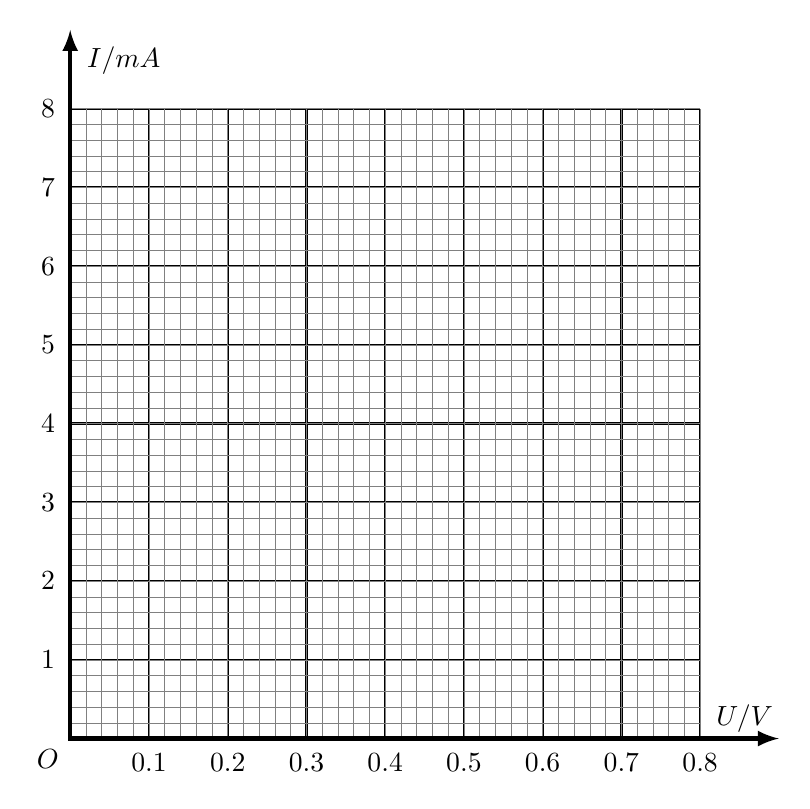
\begin{tikzpicture}
\draw[thick] (0,0) grid (8,8);
\draw[step=0.2cm,gray,very thin] (0,0) grid (8,8);

\draw[ultra thick,latex-latex] (9,0) node [above left=-2pt] {$ U/V $} -- (0,0) node [below left ] {$ O $} -- (0,9) node [below right=2pt] {$ I/mA $} ;



\foreach \label in {1,2,...,8}
{
\node[below=2pt] (ww) at (\label cm , 0) {$ 0.\label $}	;
\node[left=2pt] (ww) at (0, \label cm) {$ \label $}	;
}


\end{tikzpicture}
\end{figure}

\item 
根据作出的 $ I-U $ 图线可知,该元件是 \underlinegap (选填“线性”或“非线性”)元件.
\item 
在上述测量中,如果用导线代替电路中的定值电阻 $ R_{0} $,会导致的两个后果是 \underlinegap 。
\fourchoices
{电压和电流的测量误差增大}
{可能因电流过大烧坏待测元件}
{滑动变阻器允许的调节范围变小}
{待测元件两端电压的可调节范围变小}


\end{enumerate}


\tk{
\begin{enumerate}
\item
如图
\begin{center}
\includesvg[width=0.93\linewidth]{picture/svg/GZ-3-tiyou-0675} 
\end{center}
\item 
如图
\begin{center}
\includesvg[width=0.93\linewidth]{picture/svg/GZ-3-tiyou-0676} 
\end{center}
\item 
非线性
\item 
BC
\end{enumerate}
} 





\item
疫情期间“停课不停学”
,小明同学在家自主开展实验探究.用手机拍摄物体自由下落的视频,
得到分帧图片,利用图片中小球的位置来测量当地的重力加速度,实验装置如图$ a $所示.
\begin{figure}[h!]
\centering
\begin{subfigure}{0.35\linewidth}
\centering
\includesvg[width=0.7\linewidth]{picture/svg/GZ-3-tiyou-0669} 
\caption{}\label{}
\end{subfigure}
\begin{subfigure}{0.55\linewidth}
\centering
\includesvg[width=0.96\linewidth]{picture/svg/GZ-3-tiyou-0670} 
\caption{}\label{}
\end{subfigure}
\end{figure}
\begin{enumerate}
\item
家中有乒乓球、小塑料球和小钢球,其中最适合用作实验中下落物体的是 \underlinegap .
\item 
下列主要操作步骤的正确顺序是 \underlinegap .(填写各步骤前的序号)

①把刻度尺竖直固定在墙上

②捏住小球,从刻度尺旁静止释放

③手机固定在三角架上,调整好手机镜头的位置

④打开手机摄像功能,开始摄像

\item 
停止摄像,从视频中截取三帧图片,图片中的小球和刻度如图$ 2 $所示.已知所截取的图片相邻两
帧之间的时间间隔为 $ \frac{ 1 }{ 6 } \ s $,刻度尺的分度值是 $ 1 \ mm $,由此测得重力加速度为 \underlinegap $ m/s^{2} $.

\item 
在某次实验中,小明释放小球时手稍有晃动,视频显示小球下落时偏离了竖直方向.从该视频中截取图
片, \underlinegap (选填“仍能”或“不能”)用($ 3 $)问中的方法测出重力加速度.

\end{enumerate}


\tk{
\begin{enumerate}
\item
小钢球 
\item 
①③④② 
\item 
$ 9.6 $($ 9.5 \sim 9.7 $都算对) 
\item 
仍能	
\end{enumerate}
} 








\gaokaoxx{$ 3-5 $}



\item 
\begin{enumerate}
\item
“测温枪”
(学名“红外线辐射测温仪”)具有响应快、非接触和操作方便等优点.它是根据黑体辐射规
律设计出来的,能将接收到的人体热辐射转换成温度显示.若人体温度升高,则人体热辐射强度 $ I $ 及其极大
值对应的波长 $ \lambda $ 的变化情况是 \underlinegap .
\fourchoices
{$ I $增大, $ \lambda $ 增大}
{$ I $ 增大, $ \lambda $ 减小}
{$ I $ 减小, $ \lambda $ 增大}
{$ I $ 减小, $ \lambda $ 减小}

\tk{B} 





\item 
大量处于某激发态的氢原子辐射出多条谱线,其中最长和最短波长分别为 $ \lambda_{1} $ 和 $ \lambda_{2} $,则该激发态与基
态的能量差为 \underlinegap ,波长为 $ \lambda_{1} $ 的光子的动量为 \underlinegap .(已知普朗克常量为 $ h $,光速为 $ c $)

\tk{$\frac{h c}{\lambda_{2}} \quad \frac{h}{\lambda_{1}}$} 





\item 
一只质量为 $ 1.4 \ kg $ 的乌贼吸入 $ 0.1 \ kg $ 的水,静止在水中.遇到危险时,它在极短时间内把吸入的水向后
全部喷出,以 $ 2 \ m/s $ 的速度向前逃窜.求该乌贼喷出的水的速度大小 $ v $.

\banswer{
$v=28 \ m / s$
}





\end{enumerate}









\newpage

\gaokaoxx{$ 3-3 $}

\item 
\begin{enumerate}
\item
玻璃的出现和使用在人类生活里已有四千多年的历史,它是一种非晶体.下列关于玻璃的说法正确的有 \underlinegap .
\fourchoices
{没有固定的熔点}
{天然具有规则的几何形状}
{沿不同方向的导热性能相同}
{分子在空间上周期性排列}

\tk{AC} 





\item 
一瓶酒精用了一些后,把瓶盖拧紧,不久瓶内液面上方形成了酒精的饱和汽,此时 \underlinegap (选填“有”
或“没有”
)酒精分子从液面飞出.当温度升高时,瓶中酒精饱和汽的密度 \underlinegap (选填“增大”
“减小”或“不
变”).

\tk{有 \quad 增大} 





\item 
一定质量的理想气体从状态 $ A $ 经状态 $ B $ 变化到状态 $ C $,其 $ p-\frac{1}{V} $
图象如图所示,求该过程中气体吸收
的热量 $ Q $.
\begin{figure}[h!]
\flushright
\includesvg[width=0.25\linewidth]{picture/svg/GZ-3-tiyou-0671}
\end{figure}

\banswer{
$Q=2 \times 10^{5} \ J$
}





\end{enumerate}




\gaokaoxx{$ 3-4 $}



\item 

\begin{enumerate}
\item
电磁波广泛应用在现代医疗中.下列属于电磁波应用的医用器械有 \underlinegap .
\fourchoices
{杀菌用的紫外灯}
{拍胸片的 $ X $ 光机}
{治疗咽喉炎的超声波雾化器}
{检查血流情况的“彩超”机}

\tk{AB} 





\item 
我国的光纤通信技术处于世界领先水平.光纤内芯(内层玻璃)的折射率比外套(外层玻璃)的
\underlinegap (选填“大”或“小”
).某种光纤的内芯在空气中全反射的临界角为 $ 43 ^{ \circ } $,则该内芯的折射率为 \underlinegap .(取
$ \sin 43 ^{ \circ } =0.68, \cos 43 ^{ \circ } =0.73 $,结果保留 $ 2 $ 位有效数字)


\tk{大 \quad 1.5} 





\item 
国际宇航联合会将 $ 2020 $ 年度“世界航天奖”授予我国“嫦娥四号”任务团队.“嫦娥四号”任务创造
了多项世界第一.在探月任务中,
“玉兔二号”月球车朝正下方发射一束频率为 $ f $ 的电磁波,该电磁波分别在
月壤层的上、下表面被反射回来,反射波回到“玉兔二号”的时间差为 $ \Delta t $.已知电磁波在月壤层中传播的波
长为 $ \lambda $,求该月壤层的厚度 $ d $.

\banswer{
$d=\frac{f \lambda \Delta t}{2}$
}





\end{enumerate}



\gaokaojs



\item
如图所示,电阻为 $ 0.1 \ \Omega $ 的正方形单匝线圈 $ abcd $ 的边长为 $ 0.2 \ m $, $ bc $ 边与匀强磁场边缘重合.
磁场的宽度等于线圈的边长,磁感应强度大小为 $ 0.5 \ T $.在水平拉力作用下,线圈以 $ 8 \ m/s $ 的速度向右穿过磁
场区域.求线圈在上述过程中:
\begin{enumerate}
\item
感应电动势的大小 $ E $;
\item 
所受拉力的大小 $ F $;
\item 
感应电流产生的热量 $ Q $.

\end{enumerate}
\begin{figure}[h!]
\flushright
\includesvg[width=0.33\linewidth]{picture/svg/GZ-3-tiyou-0672}
\end{figure}

\banswer{
\begin{enumerate}
\item
$E=0.8 \ V$	
\item 	
$F=0.8 \ N$
\item 
$Q=0.32 \ J$	
\end{enumerate}
}





\item
如图所示,鼓形轮的半径为 $ R $,可绕固定的光滑水平轴 $ O $ 转动.在轮上沿相互垂直的直径方向固
定四根直杆,杆上分别固定有质量为 $ m $ 的小球,球与 $ O $ 的距离均为 $ 2R $.在轮上绕有长绳,绳上悬挂着质量
为 $ M $ 的重物.重物由静止下落,带动鼓形轮转动.重物落地后鼓形轮匀速转动,转动的角速度为 $ \omega $.绳与轮之
间无相对滑动,忽略鼓形轮、直杆和长绳的质量,不计空气阻力,重力加速度为 $ g $.求:
\begin{enumerate}
\item
重物落地后,小球线速度的大小 $ v $;
\item 
重物落地后一小球转到水平位置 $ A $,此时该球受到杆的作用力的大小 $ F $;
\item 
重物下落的高度 $ h $.
\end{enumerate}
\begin{figure}[h!]
\flushright
\includesvg[width=0.25\linewidth]{picture/svg/GZ-3-tiyou-0673}
\end{figure}



\banswer{
\begin{enumerate}
\item
$v=2 \omega R$	
\item 
$F=\sqrt{\left(2 m \omega^{2} R\right)^{2}+(m g)^{2}}$
\item 
$h=\frac{M+16 m}{2 M g}(\omega R)^{2}$
\end{enumerate}
}






\newpage

\item
空间存在两个垂直于 $ Oxy $ 平面的匀强磁场,$ y $ 轴为两磁场的边界,磁感应强度分别为 $ 2B_{0} $、$ 3B_{0} $.
甲、乙两种比荷不同的粒子同时从原点 $ O $ 沿 $ x $ 轴正向射入磁场,速度均为 $ v $.甲第 $ 1 $ 次、第 $ 2 $ 次经过 $ y $ 轴的
位置分别为 $ P $、$ Q $,其轨迹如图所示.甲经过 $ Q $ 时,乙也恰好同时经过该点.已知甲的质量为 $ m $,电荷量为 $ q $.
不考虑粒子间的相互作用和重力影响.求:
\begin{enumerate}
\item
$ Q $ 到 $ O $ 的距离 $ d $;
\item 
甲两次经过 $ P $ 点的时间间隔 $ \Delta t $;
\item 
乙的比荷$ \frac{q}{m} $可能的最小值.
\end{enumerate}
\begin{figure}[h!]
\flushright
\includesvg[width=0.28\linewidth]{picture/svg/GZ-3-tiyou-0674}
\end{figure}



\banswer{
\begin{enumerate}
\item
$d=\frac{m v}{3 q B_{0}}$
\item 
$\Delta t=\frac{2 \pi m}{q B_{0}}$
\item 
比荷的最小值为 $\frac{2 q}{m}$
\end{enumerate}
}





\end{enumerate}

%

\gaokaoheader{2020}{山东卷}


\gaokaoxz


\begin{enumerate}
\item
一质量为 $ m $ 的乘客乘坐竖直电梯下楼,其位移 $ s $ 与时间 $ t $ 的关系图像如图所示。乘客所受支持力的大小
用 $ F_{N} $ 表示,速度大小用 $ v $ 表示。重力加速度大小为 $ g $。以下判断正确的是 \xzanswer{D} 
\begin{figure}[h!]
\centering
\includesvg[width=0.23\linewidth]{picture/svg/GZ-3-tiyou-0729}
\end{figure}


\fourchoices
{$ 0 \sim t_{1} $ 时间内,$ v $ 增大,$ F_{N} >mg $}
{$ t_{1} \sim t_{2} $ 时间内,$ v $ 减小,$ F_{N} <mg $}
{$ t_{2} \sim t_{3} $ 时间内,$ v $ 增大,$ F_{N} <mg $}
{$ t_{2} \sim t_{3} $ 时间内,$ v $ 减小,$ F_{N} >mg $}





\item
氚核 \ce{^{3}_{1}H} 发生$ \beta $衰变成为氦核 \ce{^{3}_{2}He} 。假设含氚材料中 \ce{^{3}_{2}He} 发生$ \beta $衰变产生的电子可以全部定向移动,在 $ 3.2 \times 10^{4} \ s $ 时间内形成的平均电流为 $ 5.0 \times 10^{-8} \ A $。已知电子电荷量为 $ 1.6 \times 10^{-19} \ C $,在这段时间内发生$ \beta $衰变的
氚核 \ce{^{3}_{1}H} 的个数为 \xzanswer{B} 

\fourchoices
{$5.0 \times 10^{14}$}
{$1.0 \times 10^{16}$}
{$ 2.0 \times 10^{16}$}
{$1.0 \times 10^{18}$}






\item
双缝干涉实验装置的截面图如图所示。光源 $ S $ 到 $ S_{1} $、$ S_{2} $ 的距离相等,$ O $ 点为 $ S_{1} $、$ S_{2} $ 连线中垂线与光屏的
交点。光源 $ S $ 发出的波长为 $ \lambda $ 的光,经 $ S_{1} $ 出射后垂直穿过玻璃片传播到 $ O $ 点,经 $ S_{2} $ 出射后直接传播到
$ O $ 点,由 $ S_{1} $ 到 $ O $ 点与由 $ S_{2} $ 到 $ O $ 点,光传播的时间差为 $ \Delta t $。玻璃片厚度为 $ 10\lambda $,玻璃对该波长光的折射
率为 $ 1.5 $,空气中光速为 $ c $,不计光在玻璃片内的反射。以下判断正确的是 \xzanswer{A} 
\begin{figure}[h!]
\centering
\includesvg[width=0.3\linewidth]{picture/svg/GZ-3-tiyou-0730}
\end{figure}


\fourchoices
{$\Delta t=\frac{5 \lambda}{c}$}
{$ \Delta t=\frac{15 \lambda}{2 c}$}
{$ \Delta t=\frac{10 \lambda}{c}$}
{$ \Delta t=\frac{15 \lambda}{c}$}





\item
一列简谐横波在均匀介质中沿 $ x $ 轴负方向传播,
已知 $ x= \frac{ 5 }{ 4 } \lambda $ 处质点的振动方程为 $y=A \cos \left(\frac{2 \pi}{T} t\right)$,
则$ t= \frac{ 3 }{ 4 } T $
时刻的波形图正确的是 \xzanswer{D} 

\pfourchoices
{\includesvg[width=3.3cm]{picture/svg/GZ-3-tiyou-0731}}
{\includesvg[width=3.3cm]{picture/svg/GZ-3-tiyou-0732}}
{\includesvg[width=3.3cm]{picture/svg/GZ-3-tiyou-0733}}
{\includesvg[width=3.3cm]{picture/svg/GZ-3-tiyou-0734}}







\item
图 \subref{2020:山东:5a} 中的理想变压器原、副线圈匝数比 $ n_{1}:n_{2}=22:3 $,输入端 $ a $、$ b $ 所接电压 $ u $ 随时间 $ t $ 的变化关系如图 \subref{2020:山东:5b} 所示。灯泡 $ L $ 的电阻恒为 $ 15 \ \Omega $,额定电压为 $ 24 \ V $。定值电阻 $ R_{1} =10 \ \Omega $、$ R_{2} =5 \ \Omega $, 滑动变阻器 $ R $ 的最
大阻值为 $ 10 \ \Omega $。为使灯泡正常工作,滑动变阻器接入电路的电阻应调节为 \xzanswer{A} 

\begin{figure}[h!]
\centering
\begin{subfigure}{0.4\linewidth}
\centering
\includesvg[width=0.8\linewidth]{picture/svg/GZ-3-tiyou-0735} 
\caption{}\label{2020:山东:5a}
\end{subfigure}
\begin{subfigure}{0.4\linewidth}
\centering
\includesvg[width=0.8\linewidth]{picture/svg/GZ-3-tiyou-0736} 
\caption{}\label{2020:山东:5b}
\end{subfigure}	
\end{figure}


\fourchoices
{$ 1 \ \Omega $}
{$ 5 \ \Omega $}
{$ 6 \ \Omega $}
{$ 8 \ \Omega $}





\item
一定质量的理想气体从状态 $ a $ 开始,经 $ a \rightarrow b $、$ b \rightarrow c $、$ c \rightarrow a $ 三个过程后回到初始状态 $ a $,其 $ p-V $ 图像如图
所示。已知三个状态的坐标分别为 $ a $($ V_{0} $, $ 2p_0 $)、 $ b $($ 2V_0 $,$ p_{0} $)、$ c $($ 3V_0 $, $ 2p_0 $) 以下判断正确的是 \xzanswer{C} 
\begin{figure}[h!]
\centering
\includesvg[width=0.26\linewidth]{picture/svg/GZ-3-tiyou-0737}
\end{figure}


\fourchoices
{气体在 $ a \rightarrow b $ 过程中对外界做的功小于在 $ b \rightarrow c $ 过程中对外界做的功}
{气体在 $ a \rightarrow b $ 过程中从外界吸收的热量大于在 $ b \rightarrow c $ 过程中从外界吸收的热量}
{在 $ c \rightarrow a $ 过程中,外界对气体做的功小于气体向外界放出的热量}
{气体在 $ c \rightarrow a $ 过程中内能的减少量大于 $ b \rightarrow c $ 过程中内能的增加量}





\item
我国将在今年择机执行“天问 $ 1 $ 号”火星探测任务。质量为 $ m $ 的着陆器在着陆火星前,会在火星表面附近
经历一个时长为 $ t_{0} $、速度由 $ v_{0} $ 减速到零的过程。已知火星的质量约为地球的 $ 0.1 $ 倍,半径约为地球的 $ 0.5 $倍,地球表面的重力加速度大小为 $ g $,忽略火星大气阻力。若该减速过程可视为一个竖直向下的匀减
速直线运动,此过程中着陆器受到的制动力大小约为 \xzanswer{B} 

\fourchoices
{$m\left(0.4 g-\frac{v_{0}}{t_{0}}\right)$}
{$ m\left(0.4 g+\frac{v_{0}}{t_{0}}\right)$}
{$ m\left(0.2 g-\frac{v_{0}}{t_{0}}\right)$}
{$ m\left(0.2 g+\frac{v_{0}}{t_{0}}\right)$}






\item
如图所示,一轻质光滑定滑轮固定在倾斜木板上,质量分别为 $ m $ 和 $ 2m $ 的物块 $ A $、$ B $,通过不可伸长的轻
绳跨过滑轮连接,$ A $、$ B $ 间的接触面和轻绳均与木板平行。$ A $ 与 $ B $ 间、$ B $ 与木板间的动摩擦因数均为$ \mu $,
设最大静摩擦力等于滑动摩擦力。当木板与水平面的夹角为 $ 45 ^{ \circ } $时,物块 $ A $、$ B $ 刚好要滑动,则$ \mu $的值为 \xzanswer{C} 
\begin{figure}[h!]
\centering
\includesvg[width=0.27\linewidth]{picture/svg/GZ-3-tiyou-0738}
\end{figure}

\fourchoices
{$\frac{1}{3}$}
{$\frac{1}{4}$}
{$\frac{1}{5}$}
{$\frac{1}{6}$}








\item
截面为等腰直角三角形的三棱镜如图 \subref{2020:山东:9a} 所示。$ DE $ 为嵌在三棱镜内部紧贴 $ BB ^{\prime} C ^{\prime} C $ 面的线状单色可见光光
源,$ DE $ 与三棱镜的 $ ABC $ 面垂直,$ D $ 位于线段 $ BC $ 的中点。图 \subref{2020:山东:9b} 为图 \subref{2020:山东:9a} 中 $ ABC $ 面的正视图。三棱镜对
该单色光的折射率为 $ 2 $,只考虑由 $ DE $ 直接射向侧面 $ AA ^{\prime} C ^{\prime} C $ 的光线。下列说法正确的是 \xzanswer{AC} 
\begin{figure}[h!]
\centering
\begin{subfigure}{0.3\linewidth}
\centering
\includesvg[width=0.8\linewidth]{picture/svg/GZ-3-tiyou-0739} 
\caption{}\label{2020:山东:9a}
\end{subfigure}
\begin{subfigure}{0.3\linewidth}
\centering
\includesvg[width=0.8\linewidth]{picture/svg/GZ-3-tiyou-0740} 
\caption{}\label{2020:山东:9b}
\end{subfigure}
\end{figure}


\fourchoices
{光从 $ AA ^{\prime} C ^{\prime} C $ 面出射的区域占该侧面总面积的$ \frac{ 1 }{ 2 } $}
{光从 $ AA ^{\prime} C ^{\prime} C $ 面出射的区域占该侧面总面积的$ \frac{ 2 }{ 3 } $}
{若 $ DE $ 发出的单色光频率变小,$ AA ^{\prime} C ^{\prime} C $ 面有光出射的区域面积将增大}
{若 $ DE $ 发出的单色光频率变小,$ AA ^{\prime} C ^{\prime} C $ 面有光出射的区域面积将减小}





\item
真空中有两个固定的带正电的点电荷,电荷量不相等。一个带负电的试探电荷置于二者连线上的 $ O $ 点
时,仅在电场力的作用下恰好保持静止状态。过 $ O $ 点作两正电荷连线的垂线,以 $ O $ 点为圆心的圆与连
线和垂线分别交于 $ a $、$ c $ 和 $ b $、$ d $,如图所示。以下说法正确的是 \xzanswer{BD} 
\begin{figure}[h!]
\centering
\includesvg[width=0.39\linewidth]{picture/svg/GZ-3-tiyou-0741}
\end{figure}


\fourchoices
{$ a $ 点电势低于 $ O $ 点}
{$ b $ 点电势低于 $ c $ 点}
{该试探电荷在 $ a $ 点的电势能大于在 $ b $ 点的电势能}
{该试探电荷在 $ c $ 点的电势能小于在 $ d $ 点的电势能}






\item
如图所示,质量为 $ M $ 的物块 $ A $ 放置在光滑水平桌面上,右侧连接一固定于墙面的水平轻绳,左侧通过
一倾斜轻绳跨过光滑定滑轮与一竖直轻弹簧相连。现将质量为 $ m $ 的钩码 $ B $ 挂于弹簧下端,当弹簧处于
原长时,将 $ B $ 由静止释放,当 $ B $ 下降到最低点时(未着地),$ A $ 对水平桌面的压力刚好为零。轻绳不
可伸长,弹簧始终在弹性限度内,物块 $ A $ 始终处于静止状态。以下判断正确的是 \xzanswer{ACD} 
\begin{figure}[h!]
\centering
\includesvg[width=0.28\linewidth]{picture/svg/GZ-3-tiyou-0742}
\end{figure}


\fourchoices
{$ M<2m $}
{$ 2m<M<3 \ m $}
{在 $ B $ 从释放位置运动到最低点的过程中,所受合力对 $ B $ 先做正功后做负功}
{在 $ B $ 从释放位置运动到速度最大的过程中,$ B $ 克服弹簧弹力做的功等于 $ B $ 机械能的减少量}






\item 
如图所示,平面直角坐标系的第一和第二象限分别存在磁感应强度大小相等、方向相反且垂直于坐标
平面的匀强磁场,图中虚线方格为等大正方形。一位于 $ Oxy $ 平面内的刚性导体框 $ abcde $ 在外力作用下
以恒定速度沿 $ y $ 轴正方向运动(不发生转动)。从图示位置开始计时,$ 4 \ s $ 末 $ bc $ 边刚好进入磁场。在
此过程中,导体框内感应电流的大小为 $ I $ , $ ab $ 边所受安培力的大小为 $ F_{ab} $,二者与时间 $ t $ 的关系图像,
可能正确的是 \xzanswer{BC} 
\begin{figure}[h!]
\centering
\includesvg[width=0.28\linewidth]{picture/svg/GZ-3-tiyou-0743}
\end{figure}

\pfourchoices
{\includesvg[width=3cm]{picture/svg/GZ-3-tiyou-0744}}
{\includesvg[width=3cm]{picture/svg/GZ-3-tiyou-0745}}
{\includesvg[width=3cm]{picture/svg/GZ-3-tiyou-0746}}
{\includesvg[width=3cm]{picture/svg/GZ-3-tiyou-0747}}









\gaokaosy

\item
$ 2020 $ 年 $ 5 $ 月,我国进行了珠穆朗玛峰的高度测量,其中一种方法是通过使用重力仪测量重力
加速度,进而间接测量海拔高度。某同学受此启发就地取材设计了如下实验,测量当地重力加速度的
大小。实验步骤如下:
\begin{figure}[h!]
\centering
\begin{subfigure}{0.4\linewidth}
\centering
\includesvg[width=0.7\linewidth]{picture/svg/GZ-3-tiyou-0748} 
\caption{}\label{2020:山东:13a}
\end{subfigure}
\begin{subfigure}{0.8\linewidth}
\centering
\includesvg[width=0.8\linewidth]{picture/svg/GZ-3-tiyou-0749} 
\caption{}\label{2020:山东:13b}
\end{subfigure}
\end{figure}

\begin{enumerate}
\renewcommand{\labelenumii}{\roman{enumii}.}
\item
如图 \subref{2020:山东:13a} 所示,选择合适高度的垫块,使木板的倾角为 $ 53 ^{ \circ } $,在其上表面固定一与小物块下滑路径平行的刻度尺(图中未画出)。
\item 
调整手机使其摄像头正对木板表面,开启视频录像功能。将小物块从木板顶端释放,用手机记录
下小物块沿木板向下做加速直线运动的情况。然后通过录像的回放,选择小物块运动路径上合适的一
点作为测量参考点,得到小物块相对于该点的运动距离 $ L $ 与运动时间 $ t $ 的数据。
\item 
该同学选取部分实验数据,画出了$\frac{2 L}{t}-t$图像,利用图像数据得到小物块下滑的加速度大小为 $ 5.6 \ m/s^{2} $。
\item 
再次调节垫块,改变木板的倾角,重复实验。

\end{enumerate}


回答以下问题:
\begin{enumerate}
\item
当木板的倾角为 $ 37 ^{ \circ } $时,所绘图像如图 \subref{2020:山东:13b} 所示。由图像可得,物块过测量参考点时速度的大小为 \underlinegap 
$ m/s $;选取图线上位于坐标纸网格交叉点上的 $ A $、$ B $ 两点,利用 $ A $、$ B $ 两点数据得到小物块下滑加速
度的大小为 \underlinegap $ m/s^{2} $。(结果均保留 $ 2 $ 位有效数字)


\item 
根据上述数据,进一步分析得到当地的重力加速度大小为 \underlinegap $ m/s^{2} $。(结果保留 $ 2 $ 位有效数字,$ \sin 37 ^{ \circ } =0.60 $,$ \cos 37 ^{ \circ } =0.80 $ )


\end{enumerate}

\tk{
\begin{enumerate}
\item 
$ 0.32 $或$ 0.33 $\quad$ 3.1 $ 
\item 
$ 9.4 $	
\end{enumerate}
} 







\item
实验方案对实验测量的精度有直接的影响,某学习小组对“测量电源的电动势和内阻”的实验方
案进行了探究。实验室提供的器材有:

干电池一节(电动势约 $ 1.5 \ V $,内阻小于 $ 1 \ \Omega $);


电压表 $ V $ (量程 $ 3 \ V $,内阻约 $ 3 \ k\Omega $);


电流表 $ A $ (量程 $ 0.6 \ A $,内阻约 $ 1 \ \Omega $);


滑动变阻器 $ R $ (最大阻值为 $ 20 \ \Omega $);


定值电阻 $ R_{1} $ (阻值 $ 2 \ \Omega $);


定值电阻 $ R_{2} $ (阻值 $ 5 \ \Omega $);

开关一个,导线若干。

\begin{enumerate}
\item
该小组按照图 \subref{2020:山东:14a} 所示的电路进行实验,通过调节滑动变阻器阻值使电流表示数逐渐接近满偏,记
录此过程中电压表和电流表的示数,利用实验数据在 $ U-I $ 坐标纸上描点,如图 \subref{2020:山东:14b} 所示,结果发现电压表
示数的变化范围比较小,出现该现象的主要原因是 \underlinegap 。(单选,填正确答案标号)
\fourchoices
{电压表分流}
{干电池内阻较小}
{滑动变阻器最大阻值较小}
{电流表内阻较小}
\begin{figure}[h!]
\centering
\begin{subfigure}{0.4\linewidth}
\centering
\includesvg[width=0.7\linewidth]{picture/svg/GZ-3-tiyou-0750} 
\caption{}\label{2020:山东:14a}
\end{subfigure}
\begin{subfigure}{0.5\linewidth}
\centering
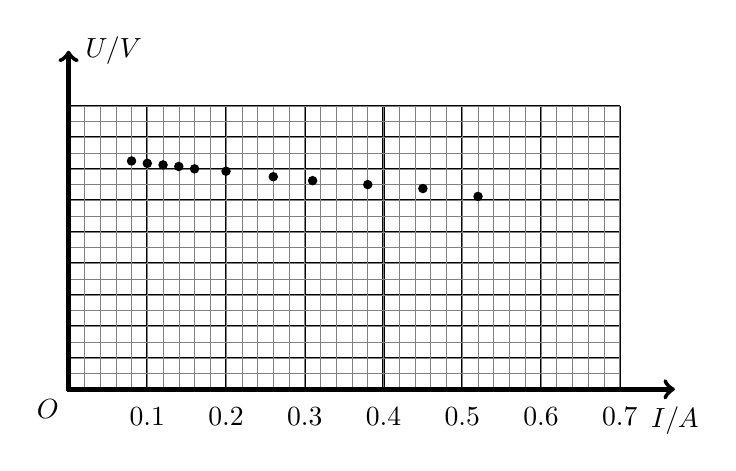
\begin{tikzpicture}
\draw[thick,xstep=1cm,ystep=0.4cm] (0,0) grid (7,3.6); %主网格
\draw[step=0.2cm,gray,very thin] (0,0) grid (7,3.6);%次网格

\draw[ultra thick,->] (-0.02,0) -- (7.7,0) node [below =2pt] {$ I/A $} ; %横坐标轴
\draw[ultra thick,->] (0,-0.02) -- (0,4.3) node [right =2pt] {$ U/V $} ; %纵坐标轴
\node at (0,0) [below left] {$ O $};%原点

\foreach \xlabel in {1,2,...,7}{ %x轴刻度
\node[below=3pt] at (\xlabel cm , 0) {$ 0.\xlabel $};
}
\foreach \ylabel in {0.4,0.8,1.2,1.6,2.0,2.4,2.8,3.2,3.6}{ %y轴刻度
\FPset\myy{\ylabel}%给计算的量赋值
\FPeval{myresult}{trunc(myy/2:1)}%表达式计算,\FPprint\myresult显示
\node[left=3pt] at (0, \ylabel cm) {$ \FPprint\myresult $};
}

\draw[fill] (0.8,2.9) circle [radius=1.5pt];
\draw[fill] (1.0,2.87) circle [radius=1.5pt];
\draw[fill] (1.2,2.85) circle [radius=1.5pt];
\draw[fill] (1.4,2.83) circle [radius=1.5pt];
\draw[fill] (1.6,2.80) circle [radius=1.5pt];
\draw[fill] (2,2.77) circle [radius=1.5pt];
\draw[fill] (2.6,2.7) circle [radius=1.5pt];
\draw[fill] (3.1,2.65) circle [radius=1.5pt];
\draw[fill] (3.8,2.6) circle [radius=1.5pt];
\draw[fill] (4.5,2.55) circle [radius=1.5pt];
\draw[fill] (5.2,2.45) circle [radius=1.5pt];
\end{tikzpicture}
\caption{}\label{2020:山东:14b}
\end{subfigure}
\end{figure}

\item 
针对电压表示数的变化范围比较小的问题,该小组利用实验室提供的器材改进了实验方案,重新
测量得到的数据如下表所示。

\begin{table}[h!]
\centering 
\begin{tabular}{|c|c|c|c|c|c|c|c|}
\hline 
序号 & 1 & 2 & 3 & 4 & 5 & 6 & 7
\\
\hline
$ I/A $ & 0.08 & 0.14 & 0.20 & 0.26 & 0.32 & 0.36 & 0.40
\\
\hline
$ U/V $& 1.35 & 1.20 & 1.05 & 0.88 & 0.73 & 0.71 & 0.52\\ 
\hline 
\end{tabular}
\end{table} 




请根据实验数据,回答以下问题:
\begin{enumerate}
\item
答题卡的坐标纸上已标出后 $ 3 $ 组数据对应的坐标点,请在答题卡的坐标纸上标出前 $ 4 $ 组数据对应的
坐标点并画出 $ U-I $ 图像。
\begin{figure}[h!]
\centering
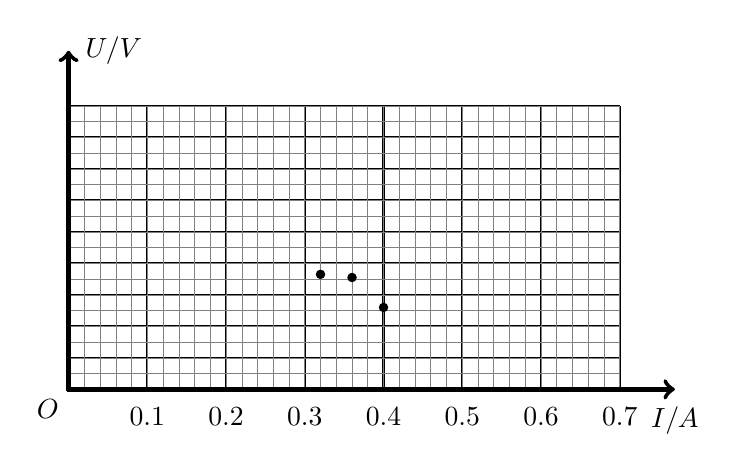
\begin{tikzpicture}
\draw[thick,xstep=1cm,ystep=0.4cm] (0,0) grid (7,3.6); %主网格
\draw[step=0.2cm,gray,very thin] (0,0) grid (7,3.6);%次网格

\draw[ultra thick,->] (-0.02,0) -- (7.7,0) node [below =2pt] {$ I/A $} ; %横坐标轴
\draw[ultra thick,->] (0,-0.02) -- (0,4.3) node [right =2pt] {$ U/V $} ; %纵坐标轴
\node at (0,0) [below left] {$ O $};%原点

\foreach \xlabel in {1,2,...,7}{ %x轴刻度
\node[below=3pt] at (\xlabel cm , 0) {$ 0.\xlabel $};
}
\foreach \ylabel in {0.4,0.8,1.2,1.6,2.0,2.4,2.8,3.2,3.6}{ %y轴刻度
\FPset\myy{\ylabel}%给计算的量赋值
\FPeval{myresult}{trunc(myy/2:1)}%表达式计算,\FPprint\myresult显示
\node[left=3pt] at (0, \ylabel cm) {$ \FPprint\myresult $};
}

\draw[fill] (4,1.04) circle [radius=1.5pt];
\draw[fill] (3.6,1.42) circle [radius=1.5pt];
\draw[fill] (3.2,1.46) circle [radius=1.5pt];
\end{tikzpicture}
\end{figure}


\item 
根据实验数据可知,所选的定值电阻为 \underlinegap (填“$ R_{1} $”或“$ R_{2} $”)。


\item 
用笔画线代替导线,请在答题卡上按照改进后的方案,将实物图连接成完整电路。
\begin{figure}[h!]
\centering
\includesvg[width=0.43\linewidth]{picture/svg/GZ-3-tiyou-1709}
\end{figure}

\end{enumerate}


\end{enumerate}


\tk{
\begin{enumerate}
\item
B	
\item 	
\begin{enumerate}
\item
如图:
\begin{center}
\includesvg[width=0.93\linewidth]{picture/svg/GZ-3-tiyou-0759} 
\end{center}
\item 
$ R_{1} $
\item 
如图:
\begin{center}
\includesvg[width=0.93\linewidth]{picture/svg/GZ-3-tiyou-1708} 
\end{center}
\end{enumerate}
\end{enumerate}
} 




\newpage
\gaokaojs

\item
中医拔罐的物理原理是利用玻璃罐内外的气压差使罐吸附在人体穴位上,进而治疗某些疾病。
常见拔罐有两种,如图所示,左侧为火罐,下端开口;右侧为抽气拔罐,下端开口,上端留有抽气阀
门。使用火罐时,先加热罐中气体,然后迅速按到皮肤上,自然降温后火罐内部气压低于外部大气压,
使火罐紧紧吸附在皮肤上。抽气拔罐是先把罐体按在皮肤上,再通过抽气降低罐内气体压强。某次使
用火罐时,罐内气体初始压强与外部大气压相同,温度为 $ 450 \ K $,最终降到 $ 300 \ K $,因皮肤凸起,内
部气体体积变为罐容积的$ \frac{20}{21} $。若换用抽气拔罐,抽气后罐内剩余气体体积变为抽气拔罐容积的$ \frac{20}{21} $,
罐内气压与火罐降温后的内部气压相同。罐内气体均可视为理想气体,忽略抽气过程中气体温度的变
化。求应抽出气体的质量与抽气前罐内气体质量的比值。
\begin{figure}[h!]
\flushright
\includesvg[width=0.35\linewidth]{picture/svg/GZ-3-tiyou-0752}
\end{figure}


\banswer{
$\frac{\Delta m}{m}=\frac{1}{3}$
}



\newpage
\item 
单板滑雪 $ U $ 型池比赛是冬奥会比赛项目,其场地可以简化为如图 \subref{2020:山东:16a} 所示的模型$ :U $ 形滑道由两
个半径相同的四分之一圆柱面轨道和一个中央的平面直轨道连接而成,轨道倾角为 $ 17.2 ^{ \circ } $。某次练习
过程中,运动员以 $ v_{M}=10 \ m/s $ 的速度从轨道边缘上的 $ M $ 点沿轨道的竖直切面 $ ABCD $ 滑出轨道,速度方
向与轨道边缘线 $ AD $ 的夹角$ \alpha =72.8 ^{ \circ } $,腾空后沿轨道边缘的 $ N $ 点进入轨道。图 \subref{2020:山东:16b} 为腾空过程左视图。
该运动员可视为质点,不计空气阻力,取重力加速度的大小 $ g=10 \ m/s^{2}, \sin 72.8 ^{ \circ } =0.96 $,$ \cos 72.8 ^{ \circ } =0.30$。求:
\begin{enumerate}
\item
运动员腾空过程中离开 $ AD $ 的距离的最大值 $ d $;
\item 
$ M $、$ N $ 之间的距离 $ L $。
\end{enumerate}
\begin{figure}[h!]
\flushright
\begin{subfigure}{0.4\linewidth}
\centering
\includesvg[width=0.85\linewidth]{picture/svg/GZ-3-tiyou-0754} 
\caption{}\label{2020:山东:16a}
\end{subfigure}
\begin{subfigure}{0.4\linewidth}
\centering
\includesvg[width=0.95\linewidth]{picture/svg/GZ-3-tiyou-0755} 
\caption{}\label{2020:山东:16b}
\end{subfigure}
\end{figure}



\banswer{
\begin{enumerate}
\item
$d=4.8 \ m$	
\item 
$L=12 \ m$
\end{enumerate}
}






\newpage
\item
某型号质谱仪的工作原理如图 \subref{2020:山东:17a} 所示。$ M $、$ N $ 为竖直放置的两金属板,两板间电压为 $ U,Q $ 板
为记录板,分界面 $ P $ 将 $ N $、$ Q $ 间区域分为宽度均为 $ d $ 的 \lmd{1} 、 \lmd{1} 两部分,$ M $、$ N $、$ P $、$ Q $ 所在平面相互平行,
$ a $、$ b $ 为 $ M $、$ N $ 上两正对的小孔。以 $ a $、$ b $ 所在直线为 $ z $ 轴, 向右为正方向,取 $ z $ 轴与 $ Q $ 板的交点 $ O $ 为坐
标原点,以平行于 $ Q $ 板水平向里为 $ x $ 轴正方向,竖直向上为 $ y $ 轴正方向,建立空间直角坐标系 $ Oxyz $。
区域 \lmd{1} 、$ \lmd{2} $内分别充满沿 $ x $ 轴正方向的匀强磁场和匀强电场,磁感应强度大小、电场强度大小分别为 $ B $和 $ E $。一质量为 $ m $,电荷量为$ +q $ 的粒子,从 $ a $ 孔飘入电场(初速度视为零),经 $ b $ 孔进入磁场,过 $ P $ 面
上的 $ c $ 点(图中未画出)进入电场,最终打到记录板 $ Q $ 上。不计粒子重力。
\begin{enumerate}
\item
求粒子在磁场中做圆周运动的半径 $ R $ 以及 $ c $ 点到 $ z $ 轴的距离 $ L $;
\item 
求粒子打到记录板上位置的 $ x $ 坐标;
\item 
求粒子打到记录板上位置的 $ y $ 坐标(用 $ R $、$ d $ 表示);
\item 
如图 \subref{2020:山东:17b} 所示,在记录板上得到三个点 $ s_{1} $、$ s_{2} $、$ s_{3} $,若这三个点是质子 \ce{^{1}_{1}H} 、氚核 \ce{^{3}_{1}H} 、氦核 \ce{^{4}_{2}He} 的位
置,请写出这三个点分别对应哪个粒子(不考虑粒子间的相互作用,不要求写出推导过程)。

\end{enumerate}
\begin{figure}[h!]
\flushright
\begin{subfigure}{0.4\linewidth}
\centering
\includesvg[width=0.8\linewidth]{picture/svg/GZ-3-tiyou-0756} 
\caption{}\label{2020:山东:17a}
\end{subfigure}
\begin{subfigure}{0.4\linewidth}
\centering
\includesvg[width=0.6\linewidth]{picture/svg/GZ-3-tiyou-0757} 
\caption{}\label{2020:山东:17b}
\end{subfigure}	
\end{figure}


\banswer{
\begin{enumerate}
\item
$R=\frac{\sqrt{2 m q U}}{q B}$ \quad $L=\frac{\sqrt{2 m q U}}{q B}-\sqrt{\frac{2 m U}{q B^{2}}-d^{2}}$
\item 
$x=\frac{m d^{2} E}{4 m U-2 q d^{2} B^{2}}$
\item 
$y=R-\sqrt{R^{2}-d^{2}}+\frac{d^{2}}{\sqrt{R^{2}-d^{2}}}$
\item 
$s_{1} $、$ s_{2}$、$ s_{3}$ 分别对应气核 ${ }_{1}^{3} \mathrm{H}$、氦去 ${ }_{2}^{4} \mathrm{He}$、质子 ${ }^{1}_{1} \mathrm{H}$ 的位置
\end{enumerate}
}





\newpage
\item
如图所示,一倾角为$ \theta $的固定斜面的底端安装一弹性挡板,$ P $、$ Q $ 两物块的质量分别为 $ m $ 和
$ 4m $,$ Q $ 静止于斜面上 $ A $ 处。某时刻,$ P $ 以沿斜面向上的速度 $ v_{0} $ 与 $ Q $ 发生弹性碰撞。$ Q $ 与斜面间的动摩
擦因数等于 $ \tan \theta $,设最大静摩擦力等于滑动摩擦力。$ P $ 与斜面间无摩擦,与挡板之间的碰撞无动能损
失。两物块均可以看作质点,斜面足够长,$ Q $ 的速度减为零之前 $ P $ 不会与之发生碰撞。重力加速度大
小为 $ g $。
\begin{enumerate}
\item
求 $ P $ 与 $ Q $ 第一次碰撞后瞬间各自的速度大小 $ v _{P1} $、$ v _{Q1} $;
\item 
求第 $ n $ 次碰撞使物块 $ Q $ 上升的高度 $ h_n $;
\item 
求物块 $ Q $ 从 $ A $ 点上升的总高度 $ H $;
\item 
为保证在 $ Q $ 的速度减为零之前 $ P $ 不会与之发生碰撞,求 $ A $ 点与挡板之间的最小距离 $ s $。
\end{enumerate}
\begin{figure}[h!]
\flushright
\includesvg[width=0.4\linewidth]{picture/svg/GZ-3-tiyou-0758}
\end{figure}

\banswer{
\begin{enumerate}
\item
$v_{P 1}=-\frac{3}{5} v_{0}$ \quad 
$v_{Q 1}=\frac{2}{5} v_{0}$
\item 
$h_{1}=\frac{v_{0}^{2}}{25 g}$ \\
$h_{2}=\frac{7}{25} \cdot \frac{v_{0}^{2}}{25 g}$ \\
$h_{3}=\left(\frac{7}{25}\right)^{2} \cdot \frac{v_{0}^{2}}{25 g}$\\
总结可知,第 $n$ 次碰撞后,物块 $Q$ 上升的高度为:\\
$h_{n}=\left(\frac{7}{25}\right)^{n-1} \cdot \frac{v_{0}^{2}}{25 g} \quad(n=1,2,3 \cdots \cdots)$
\item 
$s=\frac{(8 \sqrt{7}-13) v_{0}^{2}}{200 g \sin \theta}$
\end{enumerate}	
}





\end{enumerate}

%

\gaokaoheader{2020}{天津卷}



%一、单项选择题(每小题 $ 5 $ 分,共 $ 25 $ 分。每小题给出的四个选项中,只有一个选项是正确的)

\begin{enumerate}
%\renewcommand{\labelenumi}{\arabic{enumi}.}
% A(\Alph) a(\alph) I(\Roman) i(\roman) 1(\arabic)
%设定全局标号series=example	%引用全局变量resume=example
%[topsep=-0.3em,parsep=-0.3em,itemsep=-0.3em,partopsep=-0.3em]
%可使用leftmargin调整列表环境左边的空白长度 [leftmargin=0em]
\item
在物理学发展的进程中,人们通过对某些重要物理实验的深入观察和研究,获得正确的理论认识。下列
图示的实验中导致发现原子具有核式结构的是 \xzanswer{D} 
\pfourchoices
{\includesvg[width=4cm]{picture/svg/GZ-3-tiyou-0763}}
{\includesvg[width=4cm]{picture/svg/GZ-3-tiyou-0765}}
{\includesvg[width=4cm]{picture/svg/GZ-3-tiyou-0766}}
{\includesvg[width=4cm]{picture/svg/GZ-3-tiyou-0767}}


%题目类型:选择
%题目难度:9.5
%题目区域:光学:原子物理:电磁感应
%思想方法:
%题目特征:图像选择
%题目备注:




\item
北斗问天,国之夙愿。我国北斗三号系统的收官之星是地球静止轨道卫星,其轨道半径约为地球半径的$ 7 $倍。与近地轨道卫星相比,地球静止轨道卫星 \xzanswer{A} 
% TODO: \usepackage{graphicx} required
\begin{figure}[h!]
\centering
\includegraphics[width=0.2\linewidth]{picture/screenshot053}
\end{figure}


\fourchoices
{周期大}
{线速度大}
{角速度大}
{加速度大}

%题目类型:选择
%题目难度:8.5
%题目区域:万有引力
%思想方法:
%题目特征:材料分析
%题目备注:



\item
新冠肺炎疫情突发,中华儿女风雨同舟、守望相助,筑起了抗击疫情的巍峨长城。志愿者用非接触式体
温测量仪,通过人体辐射的红外线测量体温,防控人员用紫外线灯在无人的环境下消杀病毒,为人民健康保驾护航。红外线和紫外线相比较 \xzanswer{B} 

\fourchoices
{红外线的光子能量比紫外线的大}
{真空中红外线的波长比紫外线的长}
{真空中红外线的传播速度比紫外线的大}
{红外线能发生偏振现象,而紫外线不能}

%题目类型:选择
%题目难度:8.5
%题目区域:原子物理:电磁波
%思想方法:
%题目特征:材料分析
%题目备注:



\item
一列简谐横波沿 $ x $ 轴正方向传播,周期为 $ T $, $ t=0 $ 时的波形如图所示。 $ t=\frac{T}{4} $时 \xzanswer{C} 
\begin{figure}[h!]
\centering
\includesvg[width=0.23\linewidth]{picture/svg/GZ-3-tiyou-0768}
\end{figure}

\fourchoices
{质点 $ a $ 速度方向沿 $ y $ 轴负方向}
{质点 $ b $ 沿 $ x $ 轴正方向迁移了 $ 1 \ m $}
{质点 $ c $ 的加速度为零}
{质点 $ d $ 的位移为$ -5 \ cm $}

%题目类型:选择
%题目难度:7.5
%题目区域:机械波:波的描述
%思想方法:
%题目特征:
%题目备注:




\item
水枪是孩子们喜爱的玩具,常见的气压式水枪储水罐示意如图。从储水罐充气口充入气体,达到一定压
强后,关闭充气口。扣动扳机将阀门 $ M $ 打开,水即从枪口喷出。若在水不断喷出的过程中,罐内气体温
度始终保持不变,则气体 \xzanswer{B} 
\begin{figure}[h!]
\centering
\includesvg[width=0.23\linewidth]{picture/svg/GZ-3-tiyou-0769}
\end{figure}


\fourchoices
{压强变大}
{对外界做功}
{对外界放热}
{分子平均动能变大}

%题目类型:选择
%题目难度:7
%题目区域:热学:热力学第一定律:分子动理论
%思想方法:
%题目特征:材料分析
%题目备注:





%二、不定项选择题(每小题 $ 5 $ 分,共 $ 15 $ 分。每小题给出的四个选项中,都有多个选项是正确的。全部选对的得 $ 5 $ 分,选对但不全的得 $ 3 $ 分,选错或不答的得 $ 0 $ 分)


\item
手机无线充电是比较新颖的充电方式。如图所示,电磁感应式无线充电的原理与变压器类似,通过分别安
装在充电基座和接收能量装置上的线圈,利用产生的磁场传递能量。当充电基座上的送电线圈通入正弦式
交变电流后,就会在邻近的受电线圈中感应出电流,最终实现为手机电池充电。在充电过程中 \xzanswer{AC} 
% TODO: \usepackage{graphicx} required
\begin{figure}[h!]
\centering
\begin{subfigure}{0.4\linewidth}
\centering
\includegraphics[width=0.3\linewidth]{picture/screenshot054}
\caption{}\label{}
\end{subfigure}
\begin{subfigure}{0.4\linewidth}
\centering
\includesvg[width=0.5\linewidth]{picture/svg/GZ-3-tiyou-0770} 
\caption{}\label{}
\end{subfigure}
\end{figure}


\fourchoices
{送电线圈中电流产生的磁场呈周期性变化}
{受电线圈中感应电流产生的磁场恒定不变}
{送电线圈和受电线圈通过互感现象实现能量传递}
{手机和基座无需导线连接,这样传递能量没有损失}


%题目类型:选择
%题目难度:8.5
%题目区域:电磁感应
%思想方法:
%题目特征:材料分析
%题目备注:



\item
如图所示,在 $ Oxy $ 平面的第一象限内存在方向垂直纸面向里,磁感应强度大小为 $ B $ 的匀强磁场。一带电
粒子从 $ y $ 轴上的 $ M $ 点射入磁场,速度方向与 $ y $ 轴正方向的夹角 $ \theta=45 ^{ \circ } $。粒子经过磁场偏转后在 $ N $ 点(图
中未画出)垂直穿过 $ x $ 轴。已知 $ OM=a $,粒子电荷量为 $ q $,质量为 $ m $,重力不计。则 \xzanswer{AD} 
\begin{figure}[h!]
\centering
\includesvg[width=0.2\linewidth]{picture/svg/GZ-3-tiyou-0771}
\end{figure}


\fourchoices
{粒子带负电荷}
{粒子速度大小为$\frac{q B a}{m}$}
{粒子在磁场中运动的轨道半径为 $ a $}
{$ N $ 与 $ O $ 点相距 $ (\sqrt{2}+1)a $}


%题目类型:选择
%题目难度:6
%题目区域:磁场:磁场中带电粒子的运动
%思想方法:
%题目特征:
%题目备注:



\item
复兴号动车在世界上首次实现速度 $ 350 \ km/h $ 自动驾驶功能,成为我国高铁自主创新的又一重大标志性
成果。一列质量为 $ m $ 的动车,初速度为 $ v_{0} $,以恒定功率 $ P $ 在平直轨道上运动,经时间 $ t $ 达到该功率下的
最大速度 $ v_{m} $,设动车行驶过程所受到的阻力 $ F $ 保持不变。动车在时间 $ t $ 内 \xzanswer{BC} 
% TODO: \usepackage{graphicx} required
\begin{figure}[h!]
\centering
\includegraphics[width=0.3\linewidth]{picture/screenshot055}
\end{figure}


\fourchoices
{做匀加速直线运动}
{加速度逐渐减小}
{牵引力的功率 $ P=Fv_{m} $}
{牵引力做功 $W=\frac{1}{2} m v_{\mathrm{m}}^{2}-\frac{1}{2} m v_{0}^{2}$}

%题目类型:选择
%题目难度:6
%题目区域:能量守恒:功与功率
%思想方法:
%题目特征:材料分析
%题目备注:





\gaokaosy

\item
\begin{enumerate}
%\renewcommand{\labelenumi}{\arabic{enumi}.}
% A(\Alph) a(\alph) I(\Roman) i(\roman) 1(\arabic)
%设定全局标号series=example	%引用全局变量resume=example
%[topsep=-0.3em,parsep=-0.3em,itemsep=-0.3em,partopsep=-0.3em]
%可使用leftmargin调整列表环境左边的空白长度 [leftmargin=0em]
\item
某实验小组利用图 \subref{2020天津09a} 所示装置测定平抛运动的初速度。把白纸和复写纸叠放一起固定在竖直木板
上,在桌面上固定一个斜面,斜面的底边 $ ab $ 与桌子边缘及木板均平行。每次改变木板和桌边之间
的距离,让钢球从斜面顶端同一位置滚下,通过碰撞复写纸,在白纸上记录钢球的落点。
\begin{figure}[h!]
\centering
\begin{subfigure}{0.4\linewidth}
\centering
\includesvg[width=0.7\linewidth]{picture/svg/GZ-3-tiyou-0772} 
\caption{}\label{2020天津09a}
\end{subfigure}
\begin{subfigure}{0.4\linewidth}
\centering
\includesvg[width=0.135\linewidth]{picture/svg/GZ-3-tiyou-0773} 
\caption{}\label{2020天津09b}
\end{subfigure}
\end{figure}

\begin{enumerate}
	%\renewcommand{\labelenumi}{\arabic{enumi}.}
	% A(\Alph) a(\alph) I(\Roman) i(\roman) 1(\arabic)
	%设定全局标号series=example	%引用全局变量resume=example
	%[topsep=-0.3em,parsep=-0.3em,itemsep=-0.3em,partopsep=-0.3em]
	%可使用leftmargin调整列表环境左边的空白长度 [leftmargin=0em]
	\item
为了正确完成实验,以下做法必要的是 \underlinegap 。
\fourchoices
{实验时应保持桌面水平}
{每次应使钢球从静止开始释放}
{使斜面的底边 $ ab $ 与桌边重合}
{选择对钢球摩擦力尽可能小的斜面}

\item 
实验小组每次将木板向远离桌子的方向移动 $ 0.2 \ m $,在白纸上记录了钢球的 $ 4 $ 个落点,相邻两点之间的距离依次为 $ 15.0 \ cm $、$ 25.0 \ cm $、$ 35.0 \ cm $,示意如图 $ b $。重力加速度 $ g=10 \ m/s^{2} $,钢球平抛的初速度为 \underlinegap $ m/s $。

\item 
图 \subref{2020天津09a} 装置中,木板上悬挂一条铅垂线,其作用是 \hfullline 。

\end{enumerate}


 \tk{
\begin{enumerate}
	%\renewcommand{\labelenumi}{\arabic{enumi}.}
	% A(\Alph) a(\alph) I(\Roman) i(\roman) 1(\arabic)
	%设定全局标号series=example	%引用全局变量resume=example
	%[topsep=-0.3em,parsep=-0.3em,itemsep=-0.3em,partopsep=-0.3em]
	%可使用leftmargin调整列表环境左边的空白长度 [leftmargin=0em]
	\item
	AB 
	\item 
	$ 2 $ 
	\item 
	方便将木板调整到竖直平面	
\end{enumerate} 
} 


%题目类型:实验
%题目难度:8
%题目区域:曲线运动:平抛
%思想方法:
%题目特征:
%题目备注:



\item 
某实验小组选用以下器材测定电池组的电动势和内阻,要求测量结果尽量准确。


电压表 \qquad (量程 $ 0 \sim 3 \ V $,内阻约为 $ 3 \ k \Omega $ )

电流表 \qquad (量程 $ 0 \sim 0.6 \ A $,内阻约为 $ 1 \ \Omega $ )

滑动变阻器 \qquad ( $ 0 \sim 20 \ \Omega $,额定电流 $ 1 \ A $ )

待测电池组 \qquad (电动势约为 $ 3 \ V $,内阻约为 $ 1 \ \Omega $ )

开关、导线若干

\begin{enumerate}
	%\renewcommand{\labelenumi}{\arabic{enumi}.}
	% A(\Alph) a(\alph) I(\Roman) i(\roman) 1(\arabic)
	%设定全局标号series=example	%引用全局变量resume=example
	%[topsep=-0.3em,parsep=-0.3em,itemsep=-0.3em,partopsep=-0.3em]
	%可使用leftmargin调整列表环境左边的空白长度 [leftmargin=0em]
	\item
该小组连接的实物电路如图所示,经仔细检查,发现电路中有一条导线连接不当,这条导线对
应的编号是 \underlinegap 。
\begin{figure}[h!]
\centering
\includesvg[width=0.45\linewidth]{picture/svg/GZ-3-tiyou-0774}
\end{figure}


\item 
改正这条导线的连接后开始实验,闭合开关前,滑动变阻器的滑片 $ P $ 应置于滑动变阻器的
端 \underlinegap (填“$ a $”或者“$ b $”)

\item 
实验中发现调节滑动变阻器时,电流表读数变化明显但电压表读数变化不明显。为了解决这个问题,在电池组负极和开关之间串联一个阻值为 $ 5 \ \Omega $ 的电阻,之后该小组得到了几组电压表读数 $ U $
和对应的电流表读数 $ I $ ,
并作出 $ U-I $ 图像,如图所示。根据图像可知,
电池组的电动势为 \underlinegap $ V $,
内阻为 \underlinegap $ \Omega $。(结果均保留两位有效数字)
\begin{figure}[h!]
\centering
\includesvg[width=0.45\linewidth]{picture/svg/GZ-3-tiyou-0775}
\end{figure}

\end{enumerate}

 \tk{
\begin{enumerate}
	%\renewcommand{\labelenumi}{\arabic{enumi}.}
	% A(\Alph) a(\alph) I(\Roman) i(\roman) 1(\arabic)
	%设定全局标号series=example	%引用全局变量resume=example
	%[topsep=-0.3em,parsep=-0.3em,itemsep=-0.3em,partopsep=-0.3em]
	%可使用leftmargin调整列表环境左边的空白长度 [leftmargin=0em]
	\item
	$ 5  $
	\item 
	$ a $ 
	\item 
	$ 2.9 \quad 0.80 $
\end{enumerate} 
} 

%题目类型:实验
%题目难度:8
%题目区域:电路
%思想方法:
%题目特征:
%题目备注:



\end{enumerate}





\gaokaojs

\item
如图所示,垂直于纸面向里的匀强磁场,磁感应强度 $ B $ 随时间 $ t $ 均匀变化。正方形硬质金属
框 $ abcd $ 放置在磁场中,金属框平面与磁场方向垂直,电阻 $ R=0.1 \ \Omega $,边长 $ l=0.2 \ m $。求:
\begin{enumerate}
%\renewcommand{\labelenumi}{\arabic{enumi}.}
% A(\Alph) a(\alph) I(\Roman) i(\roman) 1(\arabic)
%设定全局标号series=example	%引用全局变量resume=example
%[topsep=-0.3em,parsep=-0.3em,itemsep=-0.3em,partopsep=-0.3em]
%可使用leftmargin调整列表环境左边的空白长度 [leftmargin=0em]
\item
在 $ t=0 $ 到 $ t=0.1 \ s $ 时间内,金属框中的感应电动势 $ E $;
\item 
$ t=0.05 \ s $ 时,金属框 $ ab $ 边受到的安培力 $ F $ 的大小和方向;
\item 
在 $ t=0 $ 到 $ t=0.1 \ s $ 时间内,金属框中电流的电功率 $ P $。

\end{enumerate}
\begin{figure}[h!]
\flushright
\begin{subfigure}{0.4\linewidth}
\centering
\includesvg[width=0.4\linewidth]{picture/svg/GZ-3-tiyou-0776} 
\caption{}\label{}
\end{subfigure}
\begin{subfigure}{0.4\linewidth}
\centering
\includesvg[width=0.6\linewidth]{picture/svg/GZ-3-tiyou-0777} 
\caption{}\label{}
\end{subfigure}
\end{figure}

\banswer{
\begin{enumerate}
%\renewcommand{\labelenumi}{\arabic{enumi}.}
% A(\Alph) a(\alph) I(\Roman) i(\roman) 1(\arabic)
%设定全局标号series=example	%引用全局变量resume=example
%[topsep=-0.3em,parsep=-0.3em,itemsep=-0.3em,partopsep=-0.3em]
%可使用leftmargin调整列表环境左边的空白长度 [leftmargin=0em]
\item
$E=0.08 \ V$
\item 
$F=0.016 \ N$方向垂直于 $a b$ 向左。
\item 
$P=0.064 \ W$
\end{enumerate}
}


%题目类型:计算
%题目难度:8
%题目区域:磁场:安培力
%思想方法:
%题目特征:
%题目备注:



\item
长为 $ l $ 的轻绳上端固定,下端系着质量为 $ m_{1} $ 的小球 $ A $,处于静止状态。$ A $ 受到一个水平瞬时
冲量后在竖直平面内做圆周运动,恰好能通过圆周轨迹的最高点。当 $ A $ 回到最低点时,质量为 $ m_{2} $ 的小
球 $ B $ 与之迎面正碰,碰后 $ A $、$ B $ 粘在一起,仍做圆周运动,并能通过圆周轨迹的最高点。不计空气阻力,重力加速度为 $ g $,求:
\begin{enumerate}
%\renewcommand{\labelenumi}{\arabic{enumi}.}
% A(\Alph) a(\alph) I(\Roman) i(\roman) 1(\arabic)
%设定全局标号series=example	%引用全局变量resume=example
%[topsep=-0.3em,parsep=-0.3em,itemsep=-0.3em,partopsep=-0.3em]
%可使用leftmargin调整列表环境左边的空白长度 [leftmargin=0em]
\item
$ A $ 受到的水平瞬时冲量 $ I $ 的大小;
\item 
碰撞前瞬间 $ B $ 的动能 $ E_{k} $ 至少多大?
\end{enumerate}


\banswer{
\begin{enumerate}
%\renewcommand{\labelenumi}{\arabic{enumi}.}
% A(\Alph) a(\alph) I(\Roman) i(\roman) 1(\arabic)
%设定全局标号series=example	%引用全局变量resume=example
%[topsep=-0.3em,parsep=-0.3em,itemsep=-0.3em,partopsep=-0.3em]
%可使用leftmargin调整列表环境左边的空白长度 [leftmargin=0em]
\item
$I=m_{1} \sqrt{5 g l}$
\item 
$E_{\mathrm{k}}=\frac{5 g l\left(2 m_{1}+m_{2}\right)^{2}}{2 m_{2}}$
\end{enumerate}
}


%题目类型:计算
%题目难度:7.5
%题目区域:动量:动量定理:动量守恒
%思想方法:
%题目特征:
%题目备注:



\newpage
\item
多反射飞行时间质谱仪是一种测量离子质量的新型实验仪器,其基本原理如图所示,从离子
源 $ A $ 处飘出的离子初速度不计,经电压为 $ U $ 的匀强电场加速后射入质量分析器。质量分析器由两个反
射区和长为 $ l $ 的漂移管(无场区域)构成,开始时反射区 $ 1 $、$ 2 $ 均未加电场,当离子第一次进入漂移管
时,两反射区开始加上电场强度大小相等、方向相反的匀强电场,其电场强度足够大,使得进入反射
区的离子能够反射回漂移管。离子在质量分析器中经多次往复即将进入反射区 $ 2 $ 时,撤去反射区的电
场,离子打在荧光屏 $ B $ 上被探测到,可测得离子从 $ A $ 到 $ B $ 的总飞行时间。设实验所用离子的电荷量均
为 $ q $,不计离子重力。
\begin{enumerate}
%\renewcommand{\labelenumi}{\arabic{enumi}.}
% A(\Alph) a(\alph) I(\Roman) i(\roman) 1(\arabic)
%设定全局标号series=example	%引用全局变量resume=example
%[topsep=-0.3em,parsep=-0.3em,itemsep=-0.3em,partopsep=-0.3em]
%可使用leftmargin调整列表环境左边的空白长度 [leftmargin=0em]
\item
求质量为 $ m $ 的离子第一次通过漂移管所用的时间 $ T_{1} $;
\item 
反射区加上电场,电场强度大小为 $ E $,求离子能进入反射区的最大距离 $ x $;
\item 
已知质量为 $ m_{0} $ 的离子总飞行时间为 $ t_{0} $,待测离子的总飞行时间为 $ t_{1} $,两种离子在质量分析器中
反射相同次数,求待测离子质量 $ m_{1} $。



\end{enumerate}
\begin{figure}[h!]
\flushright
\includesvg[width=0.85\linewidth]{picture/svg/GZ-3-tiyou-0778}
\end{figure}

\tk{
\begin{enumerate}
%\renewcommand{\labelenumi}{\arabic{enumi}.}
% A(\Alph) a(\alph) I(\Roman) i(\roman) 1(\arabic)
%设定全局标号series=example	%引用全局变量resume=example
%[topsep=-0.3em,parsep=-0.3em,itemsep=-0.3em,partopsep=-0.3em]
%可使用leftmargin调整列表环境左边的空白长度 [leftmargin=0em]
\item
$T_{1}=l\sqrt{\frac{m}{2 q U}}$
\item 
$x=\frac{U}{E}$
\item 
$m_{1}=\left(\frac{t_{1}}{t_{0}}\right)^{2} m_{0}$
\end{enumerate}
} 

%题目类型:计算
%题目难度:6
%题目区域:电场:电场中带电粒子的运动
%思想方法:
%题目特征:计算练习
%题目备注:



\end{enumerate}

%

\gaokaoheader{2020}{北京卷}





\gaokaoxz

\begin{enumerate}
\item
以下现象不属于干涉的是 \xzanswer{C} 

\fourchoices
{白光经过杨氏双缝得到彩色图样}
{白光照射肥皂膜呈现彩色图样}
{白光经过三棱镜得到彩色图样}
{白光照射水面油膜呈现彩色图样}


\item
氢原子能级示意如图。现有大量氢原子处于 $ n = 3 $ 能级上,下列说法正确的是 \xzanswer{C} 
\begin{figure}[h!]
\centering
\includesvg[width=0.23\linewidth]{picture/svg/GZ-3-tiyou-0779}
\end{figure}

\fourchoices
{这些原子跃迁过程中最多可辐射出 $ 2 $ 种频率的光子}
{从 $ n = 3 $ 能级跃迁到 $ n = 1 $ 能级比跃迁到 $ n = 2 $ 能级辐射的光子频率低}
{从 $ n =3 $ 能级跃迁到 $ n = 4 $ 能级需吸收 $ 0.66 \ eV $ 的能量}
{$ n = 3 $ 能级的氢原子电离至少需要吸收 $ 13.6 \ eV $ 的能量}


\item
随着通信技术的更新换代,无线通信使用的电磁波频率更高,频率资源更丰富,在相同时间内能够传输的信息
量更大。第 $ 5 $ 代移动通信技术(简称 $ 5G $)意味着更快的网速和更大的网络容载能力,“$ 4G $ 改变生活,$ 5G $ 改变
社会”。与 $ 4G $ 相比,$ 5G $ 使用的电磁波 \xzanswer{A} 


\fourchoices
{光子能量更大}
{衍射更明显}
{传播速度更大}
{波长更长}



\item
如图所示,一定量的理想气体从状态 $ A $ 开始,经历两个过程,先后到达状态 $ B $ 和 $ C $。有关 $ A $、$ B $ 和 $ C $ 三个状态
温度 $ T_{A} $、$ T_{B} $ 和 $ T_{C} $ 的关系,正确的是 \xzanswer{C} 
\begin{figure}[h!]
\centering
\begin{tikzpicture}[decoration={
markings,
mark=at position 0.5 with {\arrow{>}}}]
\draw[thick,gray] (0,0) grid (3,3);
\draw[gray!70,very thin,step=0.2] (0,0) grid (3,3);
\draw [->] (0,0) node [below left]{$ O $}--(0,3.5) node[right=1pt] {$ p $} ;
\draw [->] (0,0)--(3.5,0) node[above=1pt] {$ V $} ;
\draw (1,0) node[below=2pt] {$ V_{0} $};
\draw (0,1) node[left=2pt] {$ p_{0} $};
\foreach \x in {2,3}
{
\draw (\x,0) node[below=2pt] {$ \x V_{0} $};
\draw (0,\x) node[left=2pt] {$ \x p_{0} $};	
}

\draw[very thick,postaction={decorate}] (0.6,2) node[above] {$ A $} --
(2,2)node[above]{$ B $};
\draw[very thick,postaction={decorate}] (2,2)--(2,0.6)node[right]{C};
\fill (0.6,2) circle [radius=2pt];
\fill (2,2) circle [radius=2pt];
\fill (2,0.6) circle [radius=2pt];

\end{tikzpicture}
\end{figure}


\fourchoices
{$T_{A}=T_{B} $, $ T_{B}=T_{C}$}
{$ T_{A}<T_{B} $, $ T_{B}<T_{C}$}
{$ T_{A}=T_{C} $, $ T_{B}>T_{C}$}
{$ T_{A}=T_{C} $, $ T_{B}<T_{C}$}


\item
我国首次火星探测任务被命名为“天问一号”。已知火星质量约为地球质量的 $ 10 \% $,半径约为地球半径的 $ 50 \% $,
下列说法正确的是 \xzanswer{A} 

\fourchoices
{火星探测器的发射速度应大于地球的第二宇宙速度}
{火星探测器的发射速度应介于地球的第一和第二宇宙速度之间}
{火星的第一宇宙速度大于地球的第一宇宙速度}
{火星表面的重力加速度大于地球表面的重力加速度}


\item
一列简谐横波某时刻波形如图$ a $所示。由该时刻开始计时,质点 $ L $ 的振动情况如图$ b $所示。下列说法正确的是 \xzanswer{B} 
\begin{figure}[h!]
\centering
\begin{subfigure}{0.4\linewidth}
\centering
\includesvg[width=0.7\linewidth]{picture/svg/GZ-3-tiyou-0782} 
\caption{}\label{}
\end{subfigure}
\begin{subfigure}{0.4\linewidth}
\centering
\includesvg[width=0.7\linewidth]{picture/svg/GZ-3-tiyou-0783} 
\caption{}\label{}
\end{subfigure}
\end{figure}


\fourchoices
{该横波沿 $ x $ 轴负方向传播}
{质点 $ N $ 该时刻向 $ y $ 轴负方向运动}
{质点 $ L $ 经半个周期将沿 $ x $ 轴正方向移动到 $ N $ 点}
{该时刻质点 $ K $ 与$ M $的速度、加速度都相同}

\item
真空中某点电荷的等势面示意如图,图中相邻等势面间电势差相等。下列说法正确的是 \xzanswer{B} 
\begin{figure}[h!]
\centering
\includesvg[width=0.23\linewidth]{picture/svg/GZ-3-tiyou-0784}
\end{figure}


\fourchoices
{该点电荷一定为正电荷}
{$ P $ 点的场强一定比 $ Q $ 点的场强大}
{$ P $ 点电势一定比 $ Q $ 点电势低}
{正检验电荷在 $ P $ 点比在 $ Q $ 点的电势能大}

\item
如图所示,在带负电荷的橡胶圆盘附近悬挂一个小磁针。现驱动圆盘绕中心轴高速旋转,小磁针发生偏转。下
列说法正确的是 \xzanswer{B} 
\begin{figure}[h!]
\centering
\includesvg[width=0.23\linewidth]{picture/svg/GZ-3-tiyou-0785}
\end{figure}


\fourchoices
{偏转原因是圆盘周围存在电场}
{偏转原因是圆盘周围产生了磁场}
{仅改变圆盘的转动方向,偏转方向不变}
{仅改变圆盘所带电荷的电性,偏转方向不变}


\item
如图所示, 理想变压器原线圈接在$u=U_{m} \sin (\omega t+\varphi)$的交流电源上, 副线圈接三个阻值相同的电阻 $ R $,不计
电表内电阻影响。闭合开关 $ S $ 后 \xzanswer{A} 
\begin{figure}[h!]
\centering
\includesvg[width=0.48\linewidth]{picture/svg/GZ-3-tiyou-0786}
\end{figure}


\fourchoices
{电流表 $ A_{2} $ 的示数减小}
{电压表 $ V_{1} $ 的示数减小}
{电压表 $ V_{2} $ 的示数不变}
{电流表 $ A_{1} $ 的示数不变}


\item
分子力 $ F $ 随分子间距离 $ r $ 的变化如图所示。将两分子从相距 $ r = r_{2} $ 处释放,仅考虑这两个分子间的作用,下列说法
正确的是 \xzanswer{D} 
\begin{figure}[h!]
\centering
\includesvg[width=0.25\linewidth]{picture/svg/GZ-3-tiyou-0787}
\end{figure}


\fourchoices
{从 $r=r_{2}$ 到 $r=r_{0}$ 分子间引力、斥力都在减小}
{从 $r=r_{2}$ 到 $r=r_{1}$ 分子力的大小先减小后增大}
{从 $r=r_{2}$ 到 $r=r_{0}$ 分子势能先减小后增大}
{从 $r=r_{2}$ 到 $r=r_{1}$ 分子动能先增大后减小}




\item
某同学利用图$ a $所示装置研究摩擦力的变化情况。实验台上固定一个力传感器,传感器用棉线拉住物块,物块放
置在粗糙的长木板上。水平向左拉木板,传感器记录的 $ F - t $ 图像如图$ b $所示。下列说法正确的是 \xzanswer{C} 
\begin{figure}[h!]
\centering
\begin{subfigure}{0.4\linewidth}
\centering
\includesvg[width=0.8\linewidth]{picture/svg/GZ-3-tiyou-0788} 
\caption{}\label{}
\end{subfigure}
\hfil
\begin{subfigure}{0.46\linewidth}
\centering
\includesvg[width=0.95\linewidth]{picture/svg/GZ-3-tiyou-0789} 
\caption{}\label{}
\end{subfigure}
\end{figure}

\fourchoices
{实验中必须让木板保持匀速运动}
{图$ b $中曲线就是摩擦力随时间的变化曲线}
{最大静摩擦力与滑动摩擦力之比约为 $ 10:7 $}
{只用图$ b $中数据可得出物块与木板间的动摩擦因数}


\item 
图$ a $表示某金属丝的电阻 $ R $ 随摄氏温度 $ t $ 变化的情况。把这段金属丝与电池、电流表串联起来(图$ b $),用这段
金属丝做测温探头,把电流表的刻度改为相应的温度刻度,就得到了一个简易温度计。下列说法正确的是 \xzanswer{B} 
\begin{figure}[h!]
\centering
\begin{subfigure}{0.4\linewidth}
\centering
\includesvg[width=0.6\linewidth]{picture/svg/GZ-3-tiyou-0790} 
\caption{}\label{}
\end{subfigure}
\begin{subfigure}{0.4\linewidth}
\centering
\includesvg[width=0.6\linewidth]{picture/svg/GZ-3-tiyou-0791} 
\caption{}\label{}
\end{subfigure}
\end{figure}

\fourchoices
{$ t_{A} $ 应标在电流较大的刻度上,且温度与电流是线性关系}
{$ t_{A} $ 应标在电流较大的刻度上,且温度与电流是非线性关系}
{$ t_{B} $ 应标在电流较大的刻度上,且温度与电流是线性关系}
{$ t_{B} $ 应标在电流较大的刻度上,且温度与电流是非线性关系}



\item
在同一竖直平面内,$ 3 $ 个完全相同的小钢球($ 1 $ 号、$ 2 $ 号、$ 3 $ 号)悬挂于同一高度;静止时小球恰能接触且悬线
平行,如图所示。在下列实验中,悬线始终保持绷紧状态,碰撞均为对心正碰。以下分析正确的是 \xzanswer{D} 
\begin{figure}[h!]
\centering
\includesvg[width=0.18\linewidth]{picture/svg/GZ-3-tiyou-0792}
\end{figure}


\fourchoices
{将 $ 1 $ 号移至高度 $ h $ 释放,碰撞后,观察到 $ 2 $ 号静止、$ 3 $ 号摆至高度 $ h $。若 $ 2 $ 号换成质量不同的小钢球,重复上述实验,$ 3 $ 号仍能摆至高度 $ h $}
{将 $ 1 $、$ 2 $ 号一起移至高度 $ h $ 释放,碰撞后,观察到 $ 1 $ 号静止,$ 2 $、$ 3 $ 号一起摆至高度 $ h $,释放后整个过程机械能和动量都守恒}
{将右侧涂胶的 $ 1 $ 号移至高度 $ h $ 释放,$ 1 $、$ 2 $ 号碰撞后粘在一起,根据机械能守恒,$ 3 $ 号仍能摆至高度 $ h $}
{将 $ 1 $ 号和右侧涂胶的 $ 2 $ 号一起移至高度 $ h $ 释放,碰撞后,$ 2 $、$ 3 $ 号粘在一起向右运动,未能摆至高度 $ h $,释放后整个过程机械能和动量都不守恒}


\item
在无风的环境里,某人在高处释放静止的篮球,篮球竖直下落;如果先让篮球以一定的角速度绕过球心的水平
轴转动(如图)再释放,则篮球在向下掉落过程中偏离竖直方向做曲线运动。其原因是,转动的篮球在运动过
程中除受重力外,还受到空气施加的阻力 $ f_{1} $ 和偏转力 $ f_{2} $。这两个力与篮球速度 $ v $ 的关系大致为: $ f_{1} = k_1 v^{2} $,
方向与篮球运动方向相反; $ f_{2} = k_2v $,方向与篮球运动方向垂直。下列说法正确的是 \xzanswer{C} 
\begin{figure}[h!]
\centering
\includesvg[width=0.4\linewidth]{picture/svg/GZ-3-tiyou-0793}
\end{figure}


\fourchoices
{$ k_{1} $、 $ k_{2} $ 是与篮球转动角速度无关的常量}
{篮球可回到原高度且角速度与释放时的角速度相同}
{人站得足够高,落地前篮球有可能向上运动}
{释放条件合适,篮球有可能在空中持续一段水平直线运动}





\gaokaosy

\item
在“探究加速度与物体受力、物体质量的关系”实验中,做如下探究:
\begin{figure}[h!]
\centering
\includesvg[width=0.73\linewidth]{picture/svg/GZ-3-tiyou-0794}
\caption{}\label{2020:北京15:1}
\end{figure}
\begin{enumerate}
\item
为猜想加速度与质量的关系,可利用图 \ref{2020:北京15:1} 所示装置进行对比实验。两小车放在水平板上,前端通过钩码
牵引,后端各系一条细线,用板擦把两条细线按在桌上,使小车静止。抬起板擦,小车同时运动,一段
时间后按下板擦,小车同时停下。对比两小车的位移,可知加速度与质量大致成反比。关于实验条件,
下列正确的是:
\underlinegap 
(选填选项前的字母)。


\threechoices
{小车质量相同,钩码质量不同}
{小车质量不同,钩码质量相同}
{小车质量不同,钩码质量不同}

\item 
某同学为了定量验证($ 1 $)中得到的初步关系,设计实验并得到小车加速度 $ a $ 与质量 $ M $ 的 $ 7 $ 组实验数据,
如下表所示。在图 \ref{2020:北京15:2} 所示的坐标纸上已经描好了 $ 6 $ 组数据点,请将余下的一组数据描在坐标纸上,并作
出$a-\frac{1}{M}$图像。
\begin{table}[h!]
\centering 
\begin{tabular}{|c|c|c|c|c|c|c|c|}
\hline 次数 & 1 & 2 & 3 & 4 & 5 & 6 & 7 \\
\hline$a /\left(m \cdot s^{-2}\right)$ & 0.62 & 0.56 & 0.48 & 0.40 & 0.32 & 0.24 & 0.15 \\
\hline$M / kg$ & 0.25 & 0.29 & 0.33 & 0.40 & 0.50 & 0.71 & 1.00 \\
\hline
\end{tabular}
\end{table} 
\begin{figure}[h!]
\centering
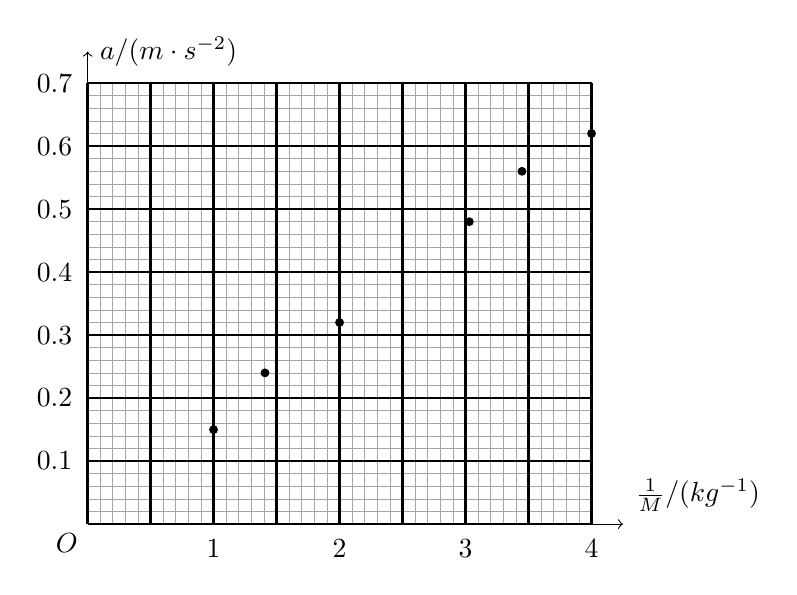
\begin{tikzpicture}[scale=0.8]

\draw[gray!70,very thin,step=0.2] (0,0) grid (8,7);
\draw[thick] (0,0) grid (8,7);
\draw [->] (0,0) node [below left]{$ O $}--(8.5,0) node[above right=1pt] {$ \frac{1}{M}/(kg^{-1}) $} ;
\draw [->] (0,0)--(0,7.5) node[right=1pt] {$ a/(m \cdot s^{-2}) $} ;


\draw (2,0) node[below=2pt] {$ 1 $};
\draw (4,0) node[below=2pt] {$ 2 $};
\draw (6,0) node[below=2pt] {$ 3 $};
\draw (8,0) node[below=2pt] {$ 4 $};


\foreach \x in {1,...,7}
{
\draw (0,\x) node[left=2pt] {$ 0.\x $};	
}



\fill (8,6.2) circle [radius=2pt];
\fill (6.8965,5.6) circle [radius=2pt];
\fill (6.06,4.8) circle [radius=2pt];
\fill (4,3.2) circle [radius=2pt];
\fill (2.816,2.4) circle [radius=2pt];
\fill (2,1.5) circle [radius=2pt];

\end{tikzpicture}
\caption{}\label{2020:北京15:2}
\end{figure}




\item 
在探究加速度与力的关系实验之前,需要思考如何测“力”。请在图 \ref{2020:北京15:3} 中画出小车受力的示意图。为了简
化“力”的测量,下列说法正确的是: \underlinegap (选填选项前的字母)
。
\begin{figure}[h!]
\centering
\includesvg[width=0.22\linewidth]{picture/svg/GZ-3-tiyou-0796}
\caption{}\label{2020:北京15:3}
\end{figure}

\fourchoices
{使小车沿倾角合适的斜面运动,小车受力可等效为只受绳的拉力}
{若斜面倾角过大,小车所受合力将小于绳的拉力}
{无论小车运动的加速度多大,砂和桶的重力都等于绳的拉力}
{让小车的运动趋近于匀速运动,砂和桶的重力才近似等于绳的拉力}

\end{enumerate}


\tk{
\begin{enumerate}
\item
B	
\item 	
如图所示
\begin{center}
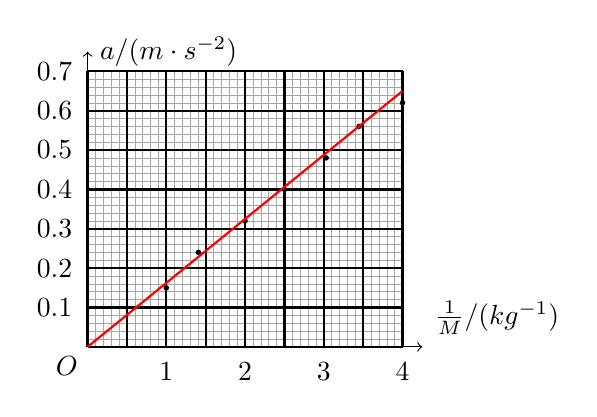
\begin{tikzpicture}[scale=0.5]
\draw[gray!70,very thin,step=0.2] (0,0) grid (8,7);
\draw[thick] (0,0) grid (8,7);
\draw [->] (0,0) node [below left]{$ O $}--(8.5,0) node[above right=1pt] {$ \frac{1}{M}/(kg^{-1}) $} ;
\draw [->] (0,0)--(0,7.5) node[right=1pt] {$ a/(m \cdot s^{-2}) $} ;


\draw (2,0) node[below=2pt] {$ 1 $};
\draw (4,0) node[below=2pt] {$ 2 $};
\draw (6,0) node[below=2pt] {$ 3 $};
\draw (8,0) node[below=2pt] {$ 4 $};


\foreach \x in {1,...,7}
{
\draw (0,\x) node[left=2pt] {$ 0.\x $};	
}



\fill (8,6.2) circle [radius=2pt];
\fill (6.8965,5.6) circle [radius=2pt];
\fill (6.06,4.8) circle [radius=2pt];
\fill (4,3.2) circle [radius=2pt];
\fill (2.816,2.4) circle [radius=2pt];
\fill (2,1.5) circle [radius=2pt];
\fill (5,4) circle [radius=2pt];
\draw[red,thick] (0,0) -- (8,6.5);
\end{tikzpicture}
\end{center}
\item 	
AD
\end{enumerate}
} 


\item 
用图 \ref{2020:北京16:1} 所示的 \subref{2020:北京16:1a} 、 \subref{2020:北京16:1b} 两种方法测量某电源的电动势和内电阻(约为 $ 1 \ \Omega $)
。其中 $ R $ 为电阻箱,电流表的内电阻约
为 $ 0.1 \ \Omega $,电压表的内电阻约为 $ 3 \ k\Omega $。
\begin{figure}[h!]
\centering
\begin{subfigure}{0.4\linewidth}
\centering
\includesvg[width=0.8\linewidth]{picture/svg/GZ-3-tiyou-0797} 
\caption{}\label{2020:北京16:1a}
\end{subfigure}
\hfil
\begin{subfigure}{0.4\linewidth}
\centering
\includesvg[width=0.8\linewidth]{picture/svg/GZ-3-tiyou-0798} 
\caption{}\label{2020:北京16:1b}
\end{subfigure}
\caption{}\label{2020:北京16:1}
\end{figure}

\begin{enumerate}
\item
利用图 \ref{2020:北京16:1} 中 \subref{2020:北京16:1a} 图实验电路测电源的电动势 $ E $ 和内电阻 $ r $,所测量的实际是图 \ref{2020:北京16:2} 中虚线框所示“等效电源”
的电动势 $ E ^{\prime} $ 和内电阻 $ r ^{\prime} $ 。若电流表内电阻用 $ R_{A} $ 表示,请你用 $ E $、$ r $ 和 $ R_{A} $ 表示出 $ E ^{\prime} $ 、 $ r ^{\prime} $ ,并简要说明理
由。
\begin{figure}[h!]
\centering
\includesvg[width=0.33\linewidth]{picture/svg/GZ-3-tiyou-0799}
\caption{}\label{2020:北京16:2}
\end{figure}



\item 
某同学利用图像分析甲、乙两种方法中由电表内电阻引起的实验误差。在图 \ref{2020:北京16:3} 中,实线是根据实验数据
(图 \subref{2020:北京16:1a} :$ U=IR $,图 \subref{2020:北京16:1b} :$\left.I=\frac{U}{R}\right)$)描点作图得到的 $ U-I $ 图像;虚线是该电源的路端电压 $ U $ 随电流 $ I $ 变化的
$ U-I $ 图像(没有电表内电阻影响的理想情况)。
\begin{figure}[h!]
\centering
\includesvg[width=0.75\linewidth]{picture/svg/GZ-3-tiyou-0800}
\caption{}\label{2020:北京16:3}
\end{figure}




在图 \ref{2020:北京16:3} 中,对应图 \subref{2020:北京16:1a} 电路分析的 $ U-I $ 图像是: \underlinegap ;对应图 \subref{2020:北京16:1b} 电路分析的 $ U-I $ 图像是: \underlinegap 。
\item 
综合上述分析,为了减小由电表内电阻引起的实验误差,本实验应选择图 \ref{2020:北京16:1} 中的 \underlinegap (填“\subref{2020:北京16:1a}”或“\subref{2020:北京16:1b}”)
。

\end{enumerate}


\tk{
\begin{enumerate}
\item
$E^{\prime}=E $,$ r ^{\prime} =r+R_{\mathrm{A}} $。理由如下:\\
将电源和电流表视为等效电源,电源电动势是电源本身具有的属性,电流表不具有产生电动
势的本领,所以等效电源的电动势仍然为
$E^{\prime}=E $,
而电流表的内阻和电动势的内阻作为等效电源的内阻,即$ r ^{\prime} =r+R_{\mathrm{A}} $。
\item 
C \quad A
\item 
\subref{2020:北京16:1b}
\end{enumerate}
} 


\gaokaojs

\item
无人机在距离水平地面高度 $ h $ 处,以速度 $ v_{0} $ 水平匀速飞行并释放一包裹,不计空气阻力,重力加速度为 $ g $。
\begin{enumerate}
\item
求包裹释放点到落地点的水平距离 $ x $;
\item 
求包裹落地时的速度大小 $ v $;
\item 
以释放点为坐标原点,初速度方向为 $ x $ 轴方向,竖直向下为 $ y $ 轴方向,建立平面直角坐标系,写出该包
裹运动的轨迹方程。
\end{enumerate}




\banswer{
\begin{enumerate}
\item
$x=v_{0} \sqrt{\frac{2 h}{g}}$
\item 
$v=\sqrt{v_{0}^{2}+2 g h}$
\item 
$y=\frac{g}{2 v_{0}^{2}} x^{2}$
\end{enumerate}
}


\vfill

\item
如图 \subref{2020:北京18:a} 所示, $ N =200 $ 匝的线圈(图中只画了 $ 2 $ 匝),电阻 $ r=2 \ \Omega $ ,其两端与一个 $ R = 48 \ \Omega $ 的电阻相连,线
圈内有指向纸内方向的磁场。线圈中的磁通量按图 \subref{2020:北京18:b} 所示规律变化。
\begin{enumerate}
\item
判断通过电阻 $ R $ 的电流方向;
\item 
求线圈产生的感应电动势 $ E $;
\item 
求电阻 $ R $ 两端的电压 $ U $。
\end{enumerate}
\begin{figure}[h!]
\flushright
\begin{subfigure}{0.3\linewidth}
\centering
\includesvg[width=0.87\linewidth]{picture/svg/GZ-3-tiyou-0805} 
\caption{}\label{2020:北京18:a}
\end{subfigure}
\begin{subfigure}{0.3\linewidth}
\centering
\includesvg[width=0.87\linewidth]{picture/svg/GZ-3-tiyou-0806} 
\caption{}\label{2020:北京18:b}
\end{subfigure}
\end{figure}


\banswer{
\begin{enumerate}
\item
$a \rightarrow b$
\item 
$ E=10 \ V $
\item 
$ U=9.6 \ V $
\end{enumerate}
}




\newpage
\item 
如图 \subref{2020:北京19:a} 所示,真空中有一长直细金属导线 $ MN $,与导线同轴放置一半径为 $ R $ 的金属圆柱面。假设导线沿径向均
匀射出速率相同的电子,已知电子质量为 $ m $,电荷量为 $ e $。不考虑出射电子间的相互作用。
\begin{enumerate}
\item
可以用以下两种实验方案测量出射电子的初速度:
\begin{enumerate}
\item
在柱面和导线之间,只加恒定电压;

\item 
在柱面内,只加与 $ MN $ 平行的匀强磁场。
\end{enumerate}


当电压为 $ U_{0} $ 或磁感应强度为 $ B_{0} $ 时,刚好没有电子到达柱面。分别计算出射电子的初速度 $ v_{0} $。

\item 
撤去柱面,沿柱面原位置放置一个弧长为 $ a $、长度为 $ b $ 的金属片,如图 \subref{2020:北京19:b} 所示。在该金属片上检测到出
射电子形成的电流为 $ I $ ,电子流对该金属片的压强为 $ p $。求单位长度导线单位时间内出射电子的总动能。

\end{enumerate}
\begin{figure}[h!]
\flushright
\begin{subfigure}{0.3\linewidth}
\centering
\includesvg[width=0.5\linewidth]{picture/svg/GZ-3-tiyou-0807} 
\caption{}\label{2020:北京19:a}
\end{subfigure}
\begin{subfigure}{0.3\linewidth}
\centering
\includesvg[width=0.5\linewidth]{picture/svg/GZ-3-tiyou-0808} 
\caption{}\label{2020:北京19:b}
\end{subfigure}
\end{figure}


\banswer{
\begin{enumerate}
\item
\begin{enumerate}
\item
当电压为$ U_{0} $时$v_{0}=\sqrt{\frac{2 e U_{0}}{m}}$
\item 
磁感应强度为$ B_{0} $时$v_{0}=\frac{B_{0} q R}{2 m}$(粒子的运动轨迹在水平面内)
\end{enumerate}
\item 
$\frac{e \pi ab p^{2} R}{m I}$
\end{enumerate}
}



\newpage
\item 
某试验列车按照设定的直线运动模式,利用计算机控制制动装置,实现安全准确地进站停车。制动装置包括电
气制动和机械制动两部分。图 \subref{2020:北京20:a} 所示为该列车在进站停车过程中设定的加速度大小 $ a $车 随速度 $ v $ 的变化曲线。
\begin{enumerate}
\item
求列车速度从 $ 20 \ m/s $ 降至 $ 3 \ m/s $ 经过的时间 $ t $ 及行进的距离 $ x $。
\item 
有关列车电气制动,可以借助图 \subref{2020:北京20:b} 模型来理解。图中水平平行金属导轨处于竖直方向的匀强磁场中,回
路中的电阻阻值为 $ R $,不计金属棒 $ MN $ 及导轨的电阻。 $ MN $ 沿导轨向右运动的过程,对应列车的电气制
动过程,可假设 $ MN $ 棒运动的速度与列车的速度、棒的加速度与列车电气制动产生的加速度成正比。列
车开始制动时,其速度和电气制动产生的加速度大小对应图 $ 1 $ 中的 $ P $ 点。论证电气制动产生的加速度大
小随列车速度变化的关系,并在图 \subref{2020:北京20:a}中画出图线。

\item 
制动过程中,除机械制动和电气制动外,列车还会受到随车速减小而减小的空气阻力。分析说明列车从$ 100 \ m/s $ 减到 $ 3 \ m/s $ 的过程中,在哪个速度附近所需机械制动最强?


\end{enumerate}
\begin{figure}[h!]
\flushright 
\begin{subfigure}{0.45\linewidth}
\centering
\includesvg[width=0.97\linewidth]{picture/svg/GZ-3-tiyou-0809}
\caption{}\label{2020:北京20:a}
\end{subfigure}
\begin{subfigure}{0.4\linewidth}
\centering
\includesvg[width=0.95\linewidth]{picture/svg/GZ-3-tiyou-0810} 
\caption{}\label{2020:北京20:b}
\end{subfigure}
\end{figure}

\banswer{
\begin{enumerate}
\item
$t=\frac{170}{7} = \approx 24.3 \ s $\\
$ x = \frac{1955}{7} = \approx 279.3 \ m$
\item 
列车电气制动产生的加速度与列车的速度成正比,为过$ P $ 点的
正比例函数,论证过程略。画出的图线如下图所示:
\begin{center}
\includesvg[width=0.93\linewidth]{picture/svg/GZ-3-tiyou-0813} 
\end{center}
\item 
由于空气阻力造成的加速度和电气制动造成的加速度之和依然与速度成正比关系,易知在$ 3 \ m/s $附近所需的机械制动最强。
\end{enumerate}
}



\end{enumerate}

%
\gaokaoheader{2020}{上海卷}





\gaokaoxz


\begin{enumerate}
\item
原子核符号 $^{17}_{8} O $ 中,$ 17 $表示 \xzanswer{D} 
\fourchoices
{电子数}
{质子数}
{中子数}
{核子数}



\item
下列电磁波中穿透能力最强的是 \xzanswer{A} 
\fourchoices
{$ \gamma $射线}
{$ X $射线}
{紫外线}
{红外线}


\item 
天然放射性元素的发现揭示了 \xzanswer{D} 
\fourchoices
{质子拥有复杂结构}
{分子拥有复杂结构}
{原子拥有复杂结构}
{原子核拥有复杂结构}



\item
下列不是基本单位的是 \xzanswer{A} 
\fourchoices
{牛顿}
{千克}
{米}
{秒}


\item 
太阳辐射的能量主要来自于太阳内部的 \xzanswer{D}

\fourchoices
{化学反应}
{裂变反应}
{链式反应}
{热核反应}




\item
一个带电粒子的电量可能为 \xzanswer{A}
\fourchoices
{$2 e$}
{$1.6 e$}
{$1.9 \times 10^{-16} e$}
{$1.6 \times 10^{-19} e$}







\item 
机械波在一个周期内传播的距离等于 \xzanswer{A} 
\fourchoices
{一个波长}
{四个波长}
{一个振幅}
{四个振幅}



\item
下列物理量中是矢量的为 \xzanswer{B} 
\fourchoices
{磁通量}
{磁感应强度}
{电流强度}
{磁通量密度}


\item 
如图将小车沿光滑斜面释放瞬间,小车的 \xzanswer{A} 
\begin{figure}[h!]
\centering
\includesvg[width=0.19\linewidth]{picture/svg/GZ-3-tiyou-1653}
\end{figure}

\fourchoices
{速度为$ 0 $}
{动能不为$ 0 $}
{加速度为$ 0 $}
{合外力为$ 0 $}



\item
如图,质量为$ M $、内壁光滑的气缸开口向下悬挂于天花板。横截面积为$ S $、质量为$ m $的活塞将一定质量的气体封闭在气缸内。平衡后,封闭气体的压强为(大气压强为$ p_{0} $) \xzanswer{C} 
\begin{figure}[h!]
\centering
\includesvg[width=0.2\linewidth]{picture/svg/GZ-3-tiyou-1654}
\end{figure}


\fourchoices
{$p_{0}-\frac{M g}{S}$}
{$p_{0}+\frac{M g}{S}$}
{$p_{0}-\frac{m g}{S}$}
{$p_{0}+\frac{m g}{S}$}



\item
如图,陀螺在平铺于水平桌面的白纸上稳定转动,若在陀螺表面滴上几滴墨水,则由于陀螺转动甩出的墨水在纸上的痕迹最接近于 \xzanswer{B} 
\begin{figure}[h!]
\centering
\includesvg[width=0.19\linewidth]{picture/svg/GZ-3-tiyou-1655}
\end{figure}

\pfourchoices
{\includesvg[width=3cm]{picture/svg/GZ-3-tiyou-1657}}
{\includesvg[width=3cm]{picture/svg/GZ-3-tiyou-1658}}
{\includesvg[width=3cm]{picture/svg/GZ-3-tiyou-1659}}
{\includesvg[width=3cm]{picture/svg/GZ-3-tiyou-1660}}






\item
小车从一斜面下滑,受到恒定阻力,下列$ v-t $图中哪个能正确反应小车的运动情况? \xzanswer{C} 

\pfourchoices
{\includesvg[width=3cm]{picture/svg/GZ-3-tiyou-1661}}
{\includesvg[width=3cm]{picture/svg/GZ-3-tiyou-1662}}
{\includesvg[width=3cm]{picture/svg/GZ-3-tiyou-1663}}
{\includesvg[width=3cm]{picture/svg/GZ-3-tiyou-1664}}




\item
如图,在上端有活塞的玻璃管底部放置一小块硝化棉,用手快速向下压活塞,可观察到硝化棉被点燃,在此过程中 \xzanswer{B} 
\begin{figure}[h!]
\centering
\includesvg[width=0.036\linewidth]{picture/svg/GZ-3-tiyou-1665}
\end{figure}

\fourchoices
{气体对外界做功,气体内能增加}
{外界对气体做功,气体内能增加}
{气体对外界做功,气体内能减少}
{外界对气体做功,气体内能减少}




\item
波速$ v=4 \ m /s $,沿$ x $轴传播的横波,某时刻质点$ a $沿$ y $轴正方向运动,则波的传播方向与频率分别为 \xzanswer{D} 
\begin{figure}[h!]
\centering
\includesvg[width=0.33\linewidth]{picture/svg/GZ-3-tiyou-1666}
\end{figure}

\fourchoices
{$ x $轴正方向,$ 2 \ Hz $}
{$ x $轴正方向,$ 0.5 \ Hz $}
{$ x $轴负方向,$ 2 \ Hz $}
{$ x $轴负方向,$ 0.5 \ Hz $}





\item
如图,在负点电荷$ a $的电场中,$ M $、$ N $两点与$ a $所在处共线,两点的电场强度大小分别为$ E_M $和$ E_N $,则它们的电场强度 \xzanswer{B} 
\begin{figure}[h!]
\centering
\includesvg[width=0.5\linewidth]{picture/svg/GZ-3-tiyou-1667}
\end{figure}


\fourchoices
{方向相同, $E_{M}>E_{N}$}
{方向相反, $E_{M}>E_{N}$}
{方向相同, $E_{M}<E_{N}$}
{方向相反,$E_{M}<E_{N}$}





\item
质量为$ 2.0 \times 10^{5} \ kg $的火箭,发射时受到竖直向上、大小为$ 6.0 \times 10^{6} \ N $的推力,加速度大小为(不要忽略重力,$ g=10 \ m/s^{2} $) \xzanswer{C} 
\fourchoices
{$ 4.0 \ m/s^{2} $}
{$ 12 \ m/s^{2} $}
{$ 20 \ m/s^{2} $}
{$ 30 \ m/s^{2} $}




\item
阻值分别为$ 2 \ \Omega $、$ 4 \ \Omega $、$ 8 \ \Omega $的三个电阻$ R_{1} $,$ R_{2} $,$ R_{3} $如图所示连接,电路中$ ab $两点间电压恒定,当$ R_{1} $功率为$ 2 \ W $时,$ R_{3} $的功率为 \xzanswer{A} 
\begin{figure}[h!]
\centering
\includesvg[width=0.38\linewidth]{picture/svg/GZ-3-tiyou-1668}
\end{figure}

\fourchoices
{$ 0.5 \ W $}
{$ 1 \ W $}
{$ 4 \ W $}
{$ 8 \ W $}




\item
已知有三个力可以达成力的平衡,以下哪组是不可能的 \xzanswer{C} 

\fourchoices
{$ 4 \ N $,$ 7 \ N $,$ 8 \ N $}
{$ 1 \ N $,$ 8 \ N $,$ 8 \ N $}
{$ 1 \ N $,$ 4 \ N $,$ 6 \ N $}
{$ 1 \ N $,$ 4 \ N $,$ 5 \ N $}



\item 
列车沿平直轨道匀速行驶,车厢光滑地板上有一个相对列车静止的物体,当列车刹车过程中,物体相对轨道 \xzanswer{A} 

\fourchoices
{向前匀速运动}
{向后匀速运动}
{向前加速运动}
{向后加速运动}



\item 
如图,螺线管与电流表组成闭合回路,不能使电流表指针偏转的是(忽略地磁影响) \xzanswer{D} 
\begin{figure}[h!]
\centering
\includesvg[width=0.23\linewidth]{picture/svg/GZ-3-tiyou-1669}
\end{figure}

\fourchoices
{螺线管不动,磁铁向上运动}
{螺线管不动,磁铁向左运动}
{磁铁不动,螺线管向上运动}
{磁铁与螺线管以相同速度一起运动}





\item
洗衣机脱水桶上螺丝旋转半径为$ 0.2 \ m $,转速为$ 1200 \ r/min $,小螺丝转动周期和线速度大小分别为 \xzanswer{A} 

\fourchoices
{$ 0.05 \ s $,$ 8 \pi m/s $}
{$ 20 \ s $,$ 8 \pi m/s $}
{$ 0.05 \ s $,$ 16 \pi m/s $}
{$ 20 \ s $,$ 16 \pi m/s $}



\item
如图,质量为$ m $的小球,自井台上方$ H $高处,由静止释放。井深为$ h $,以井台为零势能面,小球落至井底时的的机械能为(不计阻力) \xzanswer{C} 
\begin{figure}[h!]
\centering
\includesvg[width=0.23\linewidth]{picture/svg/GZ-3-tiyou-1670}
\end{figure}

\fourchoices
{$ mgh $}
{$ mg ( H-h $) }
{$ mgH $}
{$ mg ( H+h) $}




\item
电动机以$ v $,竖直匀速提升质量为$ m $的物体时,测得电动机两端电压为$ U $,通过电动机的电流为$ I $,则电动机的效率为 \xzanswer{D} 


\fourchoices
{$\frac{U I}{m g v}$}
{$\frac{U I}{m g}$}
{$\frac{m g}{U I}$}
{$\frac{m g v}{U I}$}




\item
在磁场强度为$ B $的匀强磁场中,通过面积为$ S $的矩形面的磁通量大小不可能是 \xzanswer{D} 

\fourchoices
{$ 0 $}
{$ BS $}
{$ 0.5BS $}
{$ 2BS $}





\item
一物体在地面附近以小于$ g $的加速度沿竖直方向匀加速下降,运动过程中物体 \xzanswer{C} 

\fourchoices
{动能增大,机械能增大}
{动能减小,机械能增大}
{动能增大,机械能减小}
{动能减小,机械能减小}




\item
在匀强磁场中,长为$ 10 \ cm $的直导线与磁场方向垂直。当其通有$ 10 \ A $电流时,受到的磁场力大小为$ 0.2 \ N $,则该磁场的磁感应强度大小为 \xzanswer{C} 

\fourchoices
{$ 0.01 \ T $}
{$ 0.02 \ T $}
{$ 0.2 \ T $}
{$ 5 \ T $}




\item
地球在公转轨道的近日点和远日点的加速度 \xzanswer{D} 

\fourchoices
{大小相同,方向相同}
{大小不同,方向相同}
{大小相同,方向不同}
{大小不同,方向不同}




\item
质量为$ 0.1 \ kg $的小球做自由落体运动,下落前$ 2 \ s $内重力的平均功率和$ 2 \ s $末重力的瞬时功率分别为 \xzanswer{B} 

\fourchoices
{$ 10 \ W $,$ 10 \ W $}
{$ 10 \ W $,$ 20 \ W $}
{$ 20 \ W $,$ 10 \ W $}
{$ 20 \ W $,$ 20 \ W $}



\item
如图,$ O $为平衡位置,小球在$ B $、$ C $间做无摩擦往复运动。由$ B $向$ O $运动的过程中,振子的 \xzanswer{C} 
\begin{figure}[h!]
\centering
\includesvg[width=0.25\linewidth]{picture/svg/GZ-3-tiyou-1671}
\end{figure}

\fourchoices
{动能增大,势能增大}
{动能减小,势能增大}
{动能增大,势能减小}
{动能减小,势能减小}


\item 
下列选项中,能正确描述某种气体分子速率分布规律的是 \xzanswer{A} 

\pfourchoices
{\includesvg[width=4.3cm]{picture/svg/GZ-3-tiyou-1672}}
{\includesvg[width=4.3cm]{picture/svg/GZ-3-tiyou-1673}}
{\includesvg[width=4.3cm]{picture/svg/GZ-3-tiyou-1674}}
{\includesvg[width=4.3cm]{picture/svg/GZ-3-tiyou-1675}}




\item
如图,两通电直导线$ a $、$ b $平行,$ b $电流向上。两导线相互吸引,则$ a $电流在$ b $处产生的磁场方向 \xzanswer{B} 
\begin{figure}[h!]
\centering
\includesvg[width=0.13\linewidth]{picture/svg/GZ-3-tiyou-1676}
\end{figure}

\fourchoices
{向左}
{垂直纸面向里}
{向右}
{垂直纸面向外}






\item
棒$ ab $在匀强磁场中沿导轨运动时,棒中感应电流方向如图。则$ ab $棒的运动方向和螺线管内部磁场方向分别为 \xzanswer{C} 
\begin{figure}[h!]
\centering
\includesvg[width=0.23\linewidth]{picture/svg/GZ-3-tiyou-1677}
\end{figure}

\fourchoices
{向左,$ M $指向$ N $}
{向右,$ M $指向$ N $}
{向左,$ N $}
{向右,$ N $指向$ M $}



\item 
如图所示,电压$ U $恒定,灯泡$ A $、$ B $阻值不变,若滑动变阻器$ R $的滑片右移,则 \xzanswer{B} 
\begin{figure}[h!]
\centering
\includesvg[width=0.23\linewidth]{picture/svg/GZ-3-tiyou-1678}
\end{figure}

\fourchoices
{$ A $灯变亮,$ B $灯变亮}
{$ A $灯变暗,$ B $灯变亮}
{$ A $灯变亮,$ B $灯变暗}
{$ A $灯变暗,$ B $灯变暗}



\item
如图,质量为$ m $的物体静置于地面。用手缓慢提拉与物体相连的弹簧上端,使物体升高$ h $,手做功一定 \xzanswer{B} 
\begin{figure}[h!]
\centering
\includesvg[width=0.14\linewidth]{picture/svg/GZ-3-tiyou-1679}
\end{figure}

\fourchoices
{等于$ mgh $}
{大于$ mgh $}
{小于$ mgh $}
{大于$ 2 \ m gh $}




\item
固定三通管,$ AB $管竖直,$ CD $管水平,水银在管子的$ A $端封闭了一定量的气体。打开阀门,则$ A $端气体 \xzanswer{B} 
\begin{figure}[h!]
\centering
\includesvg[width=0.15\linewidth]{picture/svg/GZ-3-tiyou-1680}
\end{figure}

\fourchoices
{体积、压强均增大}
{体积减小,压强增大}
{体积、压强均减小}
{体积增大,压强减小}




\gaokaosy




\item
\begin{enumerate}
\item
在“用$ DIS $研究机械能守恒定律”的实验中,摆锤释放器的作用是保证每次释放摆锤
时,摆锤的位置 \underlinegap 和速度 \underlinegap 。


\tk{相同 \quad 为零} 

\item 
在“用$ DIS $研究温度不变时,一定质量的气体与体积的关系”的实验中,
压强传感器 \underlinegap (选填“需要”或“不需要”)调零。能描述缓慢压缩气体过程中,气体压强$ p $与$ V $间关系的图线
是 \underlinegap 。(选填“ \subref{2020上海36a} ”或“ \subref{2020上海36b} ”)
\begin{figure}[h!]
\centering
\begin{subfigure}{0.4\linewidth}
\centering
\includesvg[width=0.5\linewidth]{picture/svg/GZ-3-tiyou-1681} 
\caption{}\label{2020上海36a}
\end{subfigure}
\begin{subfigure}{0.4\linewidth}
\centering
\includesvg[width=0.5\linewidth]{picture/svg/GZ-3-tiyou-1682} 
\caption{}\label{2020上海36b}
\end{subfigure}
\end{figure}
\end{enumerate}



\tk{不需要 \quad \subref{2020上海36a} } 



\item 
在“用$ DIS $研究通电螺线管的磁感应强度”的实验中,磁传感器 \underlinegap (选填“需要”或“不需要”)调零。能描述通电螺线管内磁感应强度大小$ B $与磁传感器插入螺线管的长度$ x $间关系的图线可能是 \underlinegap 。(选填“ \subref{2020上海37a} ”或者“ \subref{2020上海37b} ”
)
\begin{figure}[h!]
\centering
\begin{subfigure}{0.4\linewidth}
\centering
\includesvg[width=0.7\linewidth]{picture/svg/GZ-3-tiyou-1683} 
\caption{}\label{2020上海37a}
\end{subfigure}
\begin{subfigure}{0.4\linewidth}
\centering
\includesvg[width=0.7\linewidth]{picture/svg/GZ-3-tiyou-1684} 
\caption{}\label{2020上海37b}
\end{subfigure}
\end{figure}


\tk{需要 \quad \subref{2020上海37b} } 




\newpage


\gaokaojs




\item 
如图,在点电荷电场中,从$ A $点由静止释放一带负电的微粒,仅受电场力的作用,微粒
\begin{enumerate}
\item
向何方向运动?
\item 
加速度大小如何变化?
\end{enumerate}
\begin{figure}[h!]
\flushright 
\includesvg[width=0.2\linewidth]{picture/svg/GZ-3-tiyou-1685}
\end{figure}

\banswer{
\begin{enumerate}
\item
向左
\item 
变大
\end{enumerate}
}



\item 
如图,长为$ 10 \ m $的光滑斜面倾角为$ 30 \degree $。质量为$ m $的物体在一沿斜面向上、大小为$ mg $的拉力作用下,由斜面底端由静止开始沿斜面向上运动。($ g $取$ 10 \ m/s^{2} $)
\begin{enumerate}
\item
求出物体运动到斜面顶端时的速度大小;
\item 
取斜面底端为零势能面,通过分析说明物体沿斜面运动过程中动能与重力势能的大小
关系。

\end{enumerate}
\begin{figure}[h!]
\flushright
\includesvg[width=0.22\linewidth]{picture/svg/GZ-3-tiyou-1686}
\end{figure}


\banswer{
\begin{enumerate}
\item
$ 10\ m/s $
\item 
$E_{k}=E_{p}$
\end{enumerate}
}



\end{enumerate}


%
\gaokaoheader{2020}{海南卷}





\gaokaoxz


\begin{enumerate}
	%\renewcommand{\labelenumi}{\arabic{enumi}.}
	% A(\Alph) a(\alph) I(\Roman) i(\roman) 1(\arabic)
	%设定全局标号series=example	%引用全局变量resume=example
	%[topsep=-0.3em,parsep=-0.3em,itemsep=-0.3em,partopsep=-0.3em]
	%可使用leftmargin调整列表环境左边的空白长度 [leftmargin=0em]
	\item
	$ 100 $年前,卢瑟福猜想在原子核内除质子外还存在着另一种粒子$ X $,后来科学家用$ \alpha $粒子轰击铍核证实了这一猜想,该核反应方程为:${ }_{2}^{4} He+{ }_{4}^{9} Be \rightarrow{ }_{6}^{12} C+{ }_{n}^{m} X$,则 \xzanswer{A}

 

\fourchoices
{$m=1, \quad n=0, \quad X$ 是中子}
{$m=1, \quad n=0, \quad X$ 是电子}
{$m=0, \quad n=1, \quad X$ 是中子}
{$m=0, \quad n=1, \quad X$ 是电子}



\item
如图,上网课时小明把手机放在斜面上,手机处于静止状态。则斜面对手机的 \xzanswer{B} 
% TODO: \usepackage{graphicx} required
\begin{figure}[h!]
	\centering
	\includegraphics[width=0.18\linewidth]{picture/screenshot092}
\end{figure}

\fourchoices
{支持力竖直向上}
{支持力小于手机所受的重力}
{摩擦力沿斜面向下}
{摩擦力大于手机所受的重力沿斜面向下的分力}



\item
图 \subref{2020海南3a} 、 \subref{2020海南3b} 分别表示两种电流的波形,其中图 \subref{2020海南3b} 所示电流按正弦规律变化,分别用$ I_{1} $和$ I_{2} $表示 \subref{2020海南3a} 和 \subref{2020海南3b} 两电流的有效值,则 \xzanswer{D} 
\begin{figure}[h!]
	\centering
	\begin{subfigure}{0.4\linewidth}
		\centering
		\includesvg[width=0.6\linewidth]{picture/svg/GZ-3-tiyou-1687} 
		\caption{}\label{2020海南3a}
	\end{subfigure}
	\begin{subfigure}{0.4\linewidth}
		\centering
		\includesvg[width=0.6\linewidth]{picture/svg/GZ-3-tiyou-1688} 
		\caption{}\label{2020海南3b}
	\end{subfigure}
\end{figure}


\fourchoices
{$I_{1}: I_{2}=2: 1$}
{$I_{1}: I_{2}=1: 2$}
{$I_{1}: I_{2}=1: \sqrt{2}$}
{$I_{1}: I_{2}=\sqrt{2}: 1$}





\item
 一车载加热器(额定电压为 $24 \ V$ )发热部分的电路如图所示, $a$ 、$ b $、$ c $ 是三个接线
端点, 设$ ab $、$ ac $、$ bc $ 间的功率分别为 $P_{ab} $、$ P_{ac} $、$ P_{bc} $, 则 \xzanswer{D} 
\begin{figure}[h!]
	\centering
	\includesvg[width=0.23\linewidth]{picture/svg/GZ-3-tiyou-1689}
\end{figure}


\fourchoices
{$P_{ab}>P_{bc}$}
{$ P_{a b}=P_{a c}$}
{$P_{ac}=P_{b c}$}
{$P_{ab}<P_{ac}$}



\item
下列说法正确的是 \xzanswer{A} 

\fourchoices
{单色光在介质中传播时,介质的折射率越大,光的传播速度越小}
{观察者靠近声波波源的过程中,接收到的声波频率小于波源频率}
{同一个双缝干涉实验中,蓝光产生的干涉条纹间距比红光的大}
{两束频率不同的光,可以产生干涉现象}





\item
如图,在一个蹄形电磁铁的两个磁极的正中间放置一根长直导线,当导线中通有垂直于纸面向里的电流$ I $时,导线所受安培力的方向为 \xzanswer{B} 
\begin{figure}[h!]
	\centering
	\includesvg[width=0.18\linewidth]{picture/svg/GZ-3-tiyou-1690}
\end{figure}

\fourchoices
{向上}
{向下}
{向左}
{向右}



\item
$ 2020 $年$ 5 $月$ 5 $日,长征五号$ B $运载火箭在中国文昌航天发射场成功首飞,将新一代载人飞船试验船送入太空,若试验船绕地球做匀速圆周运动,周期为$ T $,离地高度为$ h $,已知地球半径为$ R $,万有引力常量为$ G $,则 \xzanswer{B} 

\fourchoices
{试验船的运行速度为 $\frac{2 \pi R}{T}$}
{地球的第一宇宙速度为 $\frac{2 \pi}{T} \sqrt{\frac{(R+h)^{3}}{R}}$}
{地球的质量为 $\frac{2 \pi(R+h)^{3}}{G T^{2}}$}
{地球表面的重力加速度为 $\frac{4 \pi^{2}(R+h)^{2}}{R T^{2}}$}

\item 
太空探测器常装配离子发动机,其基本原理是将被电离的原子从发动机尾部高速喷出,从而为探测器提供推力,若某探测器质量为$ 490 \ kg $,离子以$ 30 \ km /s $的速率(远大于探测器的飞行速率)向后喷出,流量为$ 3.0 \times 10^{-3} \ g /s $,则探测器获得的平均推力大小为 \xzanswer{C} 

\fourchoices
{$ 1.47 \ N $}
{$ 0.147 \ N $}
{$ 0.09 \ N $}
{$0.009 \ N $}



\item
一列简谐横波沿$ x $轴正方向传播,波的周期为$ 0.2 \ s $,某时刻的波形如图所示.则 \xzanswer{AC} 
\begin{figure}[h!]
	\centering
	\includesvg[width=0.25\linewidth]{picture/svg/GZ-3-tiyou-1691}
\end{figure}

\fourchoices
{该波的波长为$ 8 \ m $}
{该波的波速为$ 50 \ m /s $}
{该时刻质点$ P $向$ y $轴负方向运动}
{该时刻质点$ Q $向$ y $轴负方向运动}


\item 
空间存在如图所示的静电场,$ a $、$ b $、$ c $、$ d $为电场中的四个点,则 \xzanswer{AD} 
\begin{figure}[h!]
	\centering
	\includesvg[width=0.23\linewidth]{picture/svg/GZ-3-tiyou-1692}
\end{figure}

\fourchoices
{$ a $点的场强比$ b $点的大}
{$ d $点的电势比$ c $点的低}
{质子在$ d $点的电势能比在$ c $点的小}
{将电子从$ a $点移动到$ b $点,电场力做正功}




\item
小朋友玩水枪游戏时,若水从枪口沿水平方向射出的速度大小为$ 10 \ m /s $,水射出后落到水平地面上。已知枪口离地高度为$ 1.25 \ m $,$ g=10 \ m /s^{2} $,忽略空气阻力,则射出的水 \xzanswer{BD} 

\fourchoices
{在空中的运动时间为$ 0.25 \ s $}
{水平射程为$ 5 \ m $}
{落地时的速度大小为$ 15 \ m /s $}
{落地时竖直方向的速度大小为$ 5 \ m /s $}




\item
如图,在倾角为$ \theta $的光滑斜面上,有两个物块$ P $和$ Q $,质量分别为$ m_{1} $和$ m_{2} $,用与斜面平行的轻质弹簧相连接,在沿斜面向上的恒力$ F $作用下,两物块一起向上做匀加速直线运动,则 \xzanswer{BC} 
\begin{figure}[h!]
	\centering
	\includesvg[width=0.23\linewidth]{picture/svg/GZ-3-tiyou-1693}
\end{figure}

\fourchoices
{两物块一起运动的加速度大小为 $a=\frac{F}{m_{1}+m_{2}}$}
{弹簧的弹力大小为 $T=\frac{m_{2}}{m_{1}+m_{2}} F$}
{若只增大 $m_{2}$, 两物块一起向上匀加速运动时,它们的间距变大}
{若只增大 $\theta$, 两物块一起向上匀加速运动时,它们的间距变大}








\item
如图,足够长的间距 $d=1 \ m$ 的平行光滑金属导轨 $M N $、$ P Q$ 固定在水平面内,导轨 间存在一个宽度 $L=1 m$ 的匀强磁场区域,磁感应强度大小为 $B=0.5  \ T $ ,方向如图所
示. 一根质量 $m_{a}=0.1 kg,$ 阻值 $R=0.5 \ \Omega$ 的金属棒 $a$ 以初速度 $v_{0}=4  \ m/s$ 从左端开始
沿导轨滑动,穿过磁场区域后,与另一根质量 $m_{b}=0.2 \ kg,$ 阻值 $R=0.5 \ \Omega$ 的原来静置
在导轨上的金属棒 $b$ 发生弹性碰撞,两金属棒始终与导轨垂直且接触良好,导轨电阻不计,则  \xzanswer{BD} 
\begin{figure}[h!]
	\centering
	\includesvg[width=0.43\linewidth]{picture/svg/GZ-3-tiyou-1694}
\end{figure}


\fourchoices
{金属棒$ a $第一次穿过磁场时做匀减速直线运动}
{金属棒$ a $第一次穿过磁场时回路中有逆时针方向的感应电流}
{金属棒$ a $第一次穿过磁场区域的过程中,金属棒$ b $上产生的焦耳热为$ 0.25 \ J $}
{金属棒$ a $最终停在距磁场左边界$ 0.8 \ m $处}




\gaokaosy

\item 
\begin{enumerate}
	%\renewcommand{\labelenumi}{\arabic{enumi}.}
	% A(\Alph) a(\alph) I(\Roman) i(\roman) 1(\arabic)
	%设定全局标号series=example	%引用全局变量resume=example
	%[topsep=-0.3em,parsep=-0.3em,itemsep=-0.3em,partopsep=-0.3em]
	%可使用leftmargin调整列表环境左边的空白长度 [leftmargin=0em]
	\item
滑板运动场地有一种常见的圆弧形轨道,其截面如图,某同学用一辆滑板车和手机估测轨道半径$ R $(滑板车的长度远小于轨道半径)。
\begin{figure}[h!]
	\centering
	\includesvg[width=0.23\linewidth]{picture/svg/GZ-3-tiyou-1695}
\end{figure}



主要实验过程如下: 
\begin{enumerate}
	%\renewcommand{\labelenumi}{\arabic{enumi}.}
	% A(\Alph) a(\alph) I(\Roman) i(\roman) 1(\arabic)
	%设定全局标号series=example	%引用全局变量resume=example
	%[topsep=-0.3em,parsep=-0.3em,itemsep=-0.3em,partopsep=-0.3em]
	%可使用leftmargin调整列表环境左边的空白长度 [leftmargin=0em]
	\item
用手机查得当地的重力加速度$ g $; 

\item 
找出轨道的最低点$ O $,把滑板车从$ O $点移开一小段距离至$ P $点,由静止释放,用手机测出它完成$ n $次全振动的时间$ t $,算出滑板车做往复运动的周期$ T= $ \underlinegap ; 

\item 
将滑板车的运动视为简谐运动,则可将以上测量结果代入公式$ R= $ \underlinegap (用$ T $﹑$ g $表示)计算出轨道半径。

	
\end{enumerate}


 \tk{$\frac{t}{n} \quad \frac{g t^{2}}{4 n^{2} \pi^{2}}$} 



\item 
某同学用如图 \subref{2020海南1402a} 所示的装置测量重力加速度.
\begin{figure}[h!]
	\centering
\begin{subfigure}{0.4\linewidth}
	\centering
	\includesvg[width=0.5\linewidth]{picture/svg/GZ-3-tiyou-1696} 
	\caption{}\label{2020海南1402a}
\end{subfigure}
\begin{subfigure}{0.4\linewidth}
	\centering
	\includesvg[width=0.9\linewidth]{picture/svg/GZ-3-tiyou-1697} 
	\caption{}\label{2020海南1402b}
\end{subfigure}

\end{figure}

实验器材:有机玻璃条(白色是透光部分,黑色是宽度均为$ d=1.00 \ cm $的挡光片),铁架台,数字计时器(含光电门),刻度尺. 

主要实验过程如下: 

\begin{enumerate}
	%\renewcommand{\labelenumi}{\arabic{enumi}.}
	% A(\Alph) a(\alph) I(\Roman) i(\roman) 1(\arabic)
	%设定全局标号series=example	%引用全局变量resume=example
	%[topsep=-0.3em,parsep=-0.3em,itemsep=-0.3em,partopsep=-0.3em]
	%可使用leftmargin调整列表环境左边的空白长度 [leftmargin=0em]
	\item
将光电门安装在铁架台上,下方放置承接玻璃条下落的缓冲物;

 \item 
 用刻度尺测量两挡光片间的距离,刻度尺的示数如图 \subref{2020海南1402b} 所示,读出两挡光片间的距离$ L= $ \underlinegap $ cm $; 
 
 \item 
 手提玻璃条上端使它静止在 \underlinegap 方向上,让光电门的光束从玻璃条下端的透光部分通过; 
 
 \item 
 让玻璃条自由下落,测得两次挡光的时间分别为$t_{1}=10.003 \ ms$ 和 $t_{2}=5.000 \ ms$;
 
 \item 
 根据以上测量的数据计算出重力加速度$ g= $ \underlinegap $ m/s^{2}  $(结果保留三位有效数字)。
 

\end{enumerate}


 \tk{$15.40 \quad$ 坚直 $\quad 9.74$} 





\end{enumerate}


\item 
在测量定值电阻阻值的实验中,提供的实验器材如下:电压表 $V_{1}$ (量程 $3 \ V$ ,内阻
$r_{1}=3.0  \ k \Omega$), 电压表 $V_{2}\left(\right.$ 量程 $5 \ V$, 内阻 $r_{2}=5.0 \ k \Omega$ ), 滑动变阻器 $R($ 额定电流 $1.5 \ A,$
最大阻值 $100 \ \Omega),$ 待测定值电阻 $R_{x},$ 电源 $E$ (电动势$  6.0 \ V $,内阻不计 ),单刀开关 S, 导线若干:

回答下列问题: 
\begin{enumerate}
	%\renewcommand{\labelenumi}{\arabic{enumi}.}
	% A(\Alph) a(\alph) I(\Roman) i(\roman) 1(\arabic)
	%设定全局标号series=example	%引用全局变量resume=example
	%[topsep=-0.3em,parsep=-0.3em,itemsep=-0.3em,partopsep=-0.3em]
	%可使用leftmargin调整列表环境左边的空白长度 [leftmargin=0em]
	\item
实验中滑动变阻器应采用 \underlinegap 接法(填“限流”或“分压”); 


\item 
将虚线框中的电路原理图补充完整;
\begin{figure}[h!]
	\centering
	\includesvg[width=0.25\linewidth]{picture/svg/GZ-3-tiyou-1698}
\end{figure}

\item 
根据下表中的实验数据 $\left(U_{1}, U_{2}\right.$ 分别为电压表 $V_{1}, V_{2}$ 的示数 $),$ 在图 \subref{2020海南15a} 给
出的坐标纸上补齐数据点,并绘制 $U_{2}-U_{1}$ 图像;



\begin{table}[h!]
 \centering 
\begin{tabular}{|c|c|c|c|c|c|}
	\hline 测量次数 & 1 & 2 & 3 & 4 & 5 \\
	\hline$U_{1} / \mathrm{V}$ & 1.00 & 1.50 & 2.00 & 2.50 & 3.00 \\
	\hline$U_{2} / \mathrm{V}$ & 1.61 & 2.41 & 3.21 & 4.02 & 4.82 \\
	\hline
\end{tabular}
 \end{table} 

\begin{figure}[h!]
	\centering
\begin{subfigure}{0.4\linewidth}
	\centering
	\includesvg[width=0.85\linewidth]{picture/svg/GZ-3-tiyou-1699} 
	\caption{}\label{2020海南15a}
\end{subfigure}
\begin{subfigure}{0.4\linewidth}
	\centering
	\includesvg[width=0.6\linewidth]{picture/svg/GZ-3-tiyou-1700} 
	\caption{}\label{2020海南15b}
\end{subfigure}

\end{figure}



\item 
由 $U_{2}-U_{1}$ 图像得到待测定值电阻的阻值 $R_{x}= $ \underlinegap $ \Omega$ (结果保留三位有效数字 );


\item 
完成上述实验后,若要继续采用该实验原理测定另一个定值电阻$ R_{y} $(阻值约为$ 700 \ \Omega $)的阻值,在不额外增加器材的前提下,要求实验精度尽可能高,请在图 \subref{2020海南15b} 的虚线框内画出你改进的电路图。







\end{enumerate}



 \tk{
 \begin{enumerate}
 		%\renewcommand{\labelenumi}{\arabic{enumi}.}
 		% A(\Alph) a(\alph) I(\Roman) i(\roman) 1(\arabic)
 		%设定全局标号series=example	%引用全局变量resume=example
 		%[topsep=-0.3em,parsep=-0.3em,itemsep=-0.3em,partopsep=-0.3em]
 		%可使用leftmargin调整列表环境左边的空白长度 [leftmargin=0em]
 		\item
 		分压
 		\item 
 		如图:
 		\begin{center}
 			\includesvg[width=0.7\linewidth]{picture/svg/GZ-3-tiyou-1704} 
 		\end{center}
 		\item 
 		如图:
 		\begin{center}
 			\includesvg[width=0.7\linewidth]{picture/svg/GZ-3-tiyou-1705} 
 		\end{center}
 		\item 
 		$1.83 \times 10^{3}$
 		\item 
 		如图:
 		\begin{center}
 			\includesvg[width=0.7\linewidth]{picture/svg/GZ-3-tiyou-1706} 
 		\end{center}
 \end{enumerate}
} 


\newpage

\gaokaojs


\item 
如图,圆柱形导热气缸长 $L_{0}=60 \ cm$ ,缸内用活塞(质量和厚度均不计)密闭了一
定质量的理想气体,缸底装有一个触发器$  D $,当缸内压强达到 $p=1.5 \times 10^{5} \ Pa$ 时, $D$ 被
触发,不计活塞与缸壁的摩擦。初始时,活塞位于缸口处,环境温度 $t_{0}=27 \celsius $ ,压强
$p_{0}=1.0 \times 10^{5} \ Pa$。
\begin{enumerate}
	%\renewcommand{\labelenumi}{\arabic{enumi}.}
	% A(\Alph) a(\alph) I(\Roman) i(\roman) 1(\arabic)
	%设定全局标号series=example	%引用全局变量resume=example
	%[topsep=-0.3em,parsep=-0.3em,itemsep=-0.3em,partopsep=-0.3em]
	%可使用leftmargin调整列表环境左边的空白长度 [leftmargin=0em]
	\item
	若环境温度不变,缓慢向下推活塞,求$ D $刚好被触发时,到缸底的距离; 
	\item 
	若活塞固定在缸口位置,缓慢升高环境温度,求$ D $刚好被触发时的环境温度。
	
	
	
	
	
	
\end{enumerate}
\begin{figure}[h!]
	\flushright
	\includesvg[width=0.2\linewidth]{picture/svg/GZ-3-tiyou-1701}
\end{figure}


\banswer{
\begin{enumerate}
	%\renewcommand{\labelenumi}{\arabic{enumi}.}
	% A(\Alph) a(\alph) I(\Roman) i(\roman) 1(\arabic)
	%设定全局标号series=example	%引用全局变量resume=example
	%[topsep=-0.3em,parsep=-0.3em,itemsep=-0.3em,partopsep=-0.3em]
	%可使用leftmargin调整列表环境左边的空白长度 [leftmargin=0em]
	\item
	$ 0.4 \ m $
	\item 
	$ 450 \ K $
\end{enumerate}
}






\item 
如图,光滑的四分之一圆弧轨道 $P Q$ 坚直放置,底端与一水平传送带相切,一质量
$m_{a}=1 \ kg$ 的小物项 $a$ 从圆弧轨道最高点 $P$ 由静止释放,到最低点 $Q$ 时与另一质量
$m_{b}=3 \ kg$ 小物块 $b$ 发生弹性正碰(碰撞时间极短 $)$ 。已知圆弧轨道半径 $R=0.8 \ m,$ 传
送带的长度 $L=1.25 \ m,$ 传送带以速度 $v=1 \ m/s$ 顺时针匀速转动,小物体与传送带间的动
摩擦因数 $\mu=0.2,  g=10 \ m/s^{2}$ 。求:
\begin{enumerate}
	%\renewcommand{\labelenumi}{\arabic{enumi}.}
	% A(\Alph) a(\alph) I(\Roman) i(\roman) 1(\arabic)
	%设定全局标号series=example	%引用全局变量resume=example
	%[topsep=-0.3em,parsep=-0.3em,itemsep=-0.3em,partopsep=-0.3em]
	%可使用leftmargin调整列表环境左边的空白长度 [leftmargin=0em]
	\item
	碰撞前瞬间小物块$ a $对圆弧轨道的压力大小; 
	\item 
	碰后小物块$ a $能上升的最大高度; 
	\item 
	小物块$ b $从传送带的左端运动到右端所需要的时间。
	
	
	
	
	
	
\end{enumerate}
\begin{figure}[h!]
	\flushright
	\includesvg[width=0.3\linewidth]{picture/svg/GZ-3-tiyou-1702}
\end{figure}

\banswer{
\begin{enumerate}
	%\renewcommand{\labelenumi}{\arabic{enumi}.}
	% A(\Alph) a(\alph) I(\Roman) i(\roman) 1(\arabic)
	%设定全局标号series=example	%引用全局变量resume=example
	%[topsep=-0.3em,parsep=-0.3em,itemsep=-0.3em,partopsep=-0.3em]
	%可使用leftmargin调整列表环境左边的空白长度 [leftmargin=0em]
	\item
	$ 30 \ N $
	\item 
	$ 0.2 \ m $
	\item 
	$ 1 \ s $
\end{enumerate}
}



\newpage
\item 
如图,虚线$ MN $左侧有一个正三角形$ ABC $,$ C $点在$ MN $上,$ AB $与$ MN $平行,该三角形区域内存在垂直于纸面向外的匀强磁场;$ MN $右侧的整个区域存在垂直于纸面向里的匀强磁场,一个带正电的离子(重力不计)以初速度$ v_{0} $从$ AB $的中点$ O $沿$ OC $方向射入三角形区域,偏转$ 60 \degree  $后从$ MN $上的Р点(图中未画出)进入$ MN $右侧区域,偏转后恰能回到$ O $点。已知离子的质量为$ m $,电荷量为$ q $,正三角形的边长为$ d $:
\begin{enumerate}
	%\renewcommand{\labelenumi}{\arabic{enumi}.}
	% A(\Alph) a(\alph) I(\Roman) i(\roman) 1(\arabic)
	%设定全局标号series=example	%引用全局变量resume=example
	%[topsep=-0.3em,parsep=-0.3em,itemsep=-0.3em,partopsep=-0.3em]
	%可使用leftmargin调整列表环境左边的空白长度 [leftmargin=0em]
	\item
	求三角形区域内磁场的磁感应强度;
	\item 
	求离子从$ O $点射入到返回$ O $点所需要的时间; 
	\item 
	若原三角形区域存在的是一磁感应强度大小与原来相等的恒磁场,将$ MN $右侧磁场变为一个与$ MN $相切于$ P $点的圆形匀强磁场让离子从$ P $点射入圆形磁场,速度大小仍为$ v_{0} $,方向垂直于$ BC $,始终在纸面内运动,到达$ O $点时的速度方向与$ OC $成$ 120 \degree  $角,求圆形磁场的磁感应强度。

	
\end{enumerate}
\begin{figure}[h!]
	\flushright
	\includesvg[width=0.18\linewidth]{picture/svg/GZ-3-tiyou-1703}
\end{figure}


\banswer{
\begin{enumerate}
	%\renewcommand{\labelenumi}{\arabic{enumi}.}
	% A(\Alph) a(\alph) I(\Roman) i(\roman) 1(\arabic)
	%设定全局标号series=example	%引用全局变量resume=example
	%[topsep=-0.3em,parsep=-0.3em,itemsep=-0.3em,partopsep=-0.3em]
	%可使用leftmargin调整列表环境左边的空白长度 [leftmargin=0em]
	\item
$B=\frac{2 m v_{0}}{q d}$
	\item 
$t=\frac{(11 \pi+3 \sqrt{3}) d}{3 v_{0}}$	
\item 
\begin{enumerate}
	%\renewcommand{\labelenumi}{\arabic{enumi}.}
	% A(\Alph) a(\alph) I(\Roman) i(\roman) 1(\arabic)
	%设定全局标号series=example	%引用全局变量resume=example
	%[topsep=-0.3em,parsep=-0.3em,itemsep=-0.3em,partopsep=-0.3em]
	%可使用leftmargin调整列表环境左边的空白长度 [leftmargin=0em]
	\item
若三角形$ ABC $区域磁场方向向里,圆形磁场的磁感应强度$B=\frac{6 m v_{0}}{5 q d}$
\item 
若三角形$ ABC $区域磁场方向向外,圆形磁场的磁感应强度$B=\frac{2 m v_{0}}{q d}$	
\end{enumerate}
\end{enumerate}
}









	
	
	
\end{enumerate}

%
\gaokaoheader{2020}{浙江1月选考卷}
\gaokaoxz




\begin{enumerate}
\item
以下物理量为矢量,且单位是国际单位制基本单位的是 \xzanswer{B} 


\fourchoices
{电流、$ A $}
{位移、$ m $}
{功、$ J $}
{磁感应强度、$ T $}

\item
如图所示,一对父子掰手腕,父亲让儿子获胜。若父亲对儿子的力记为 $ F_{1} $,儿子对父亲的力记为 $ F_{2} $,则 \xzanswer{B} 
\begin{figure}[h!]
\centering
\includegraphics[width=0.23\linewidth]{picture/screenshot083}
\end{figure}


\fourchoices
{$ F_{2} > F_{1} $}
{$ F_{1} $ 和 $ F_{2} $ 大小相等}
{$ F_{1} $ 先于 $ F_{2} $ 产生}
{$ F_{1} $ 后于 $ F_{2} $ 产生}


\item
如图所示,新中国成立 $ 70 $ 周年阅兵仪式上,国产武装直升机排列并保持“$ 70 $”字样编队从天安门上空整
齐飞过。甲、乙分别是编队中的两架直升机,则 \xzanswer{D} 
\begin{figure}[h!]
\centering
\includegraphics[width=0.23\linewidth]{picture/screenshot084}
\end{figure}


\fourchoices
{以甲为参考系,乙是运动 的}
{以乙为参考系,甲是运动的}
{以甲为参考系,坐在观众席上的观众都是静止的}
{以乙为参考系,“$ 70 $”字样编队中所有直升机都是静止的}


\item
下列说法正确的是 \xzanswer{D} 


\fourchoices
{$ \alpha $ 射线的穿透能力比 $ \beta $ 射线强}
{天然放射现象说明原子具有复杂的结构}
{核聚变中平均每个核子放出的能量比裂变中平均每个核子的小}
{半衰期跟放射性元素以单质或化合物形式存在无关}

\newpage
\item
如图所示,钢球从斜槽轨道末端以 $ v_{0} $ 的水平速度飞出,经过时间 $ t $ 落在斜靠的挡板 $ AB $ 中点。若钢球以 $ 2 v_{0} $
的速度水平飞出,则 \xzanswer{C} 
\begin{figure}[h!]
\centering
\includesvg[width=0.23\linewidth]{picture/svg/GZ-3-tiyou-0678}
\end{figure}

\fourchoices
{下落时间仍为 $ t $}
{下落时间为 $ 2t $}
{下落时间为 $ \sqrt{2} t $}
{落在挡板底端 $ B $ 点}



\item
小明在一根细橡胶管中灌满食盐水,两端用粗铜丝塞住管口,形成一段封闭的盐水柱。他将此盐水柱接
到电源两端,电源电动势和内阻恒定。握住盐水柱两端将它水平均匀拉伸到原长的 $ 1.2 $ 倍,若忽略温度对电
阻率的影响,则此盐水柱 \xzanswer{B} 


\fourchoices
{通过的电流增大}
{两端的电压增大}
{阻值增大为原来的 $ 1.2 $ 倍}
{电功率增大为原来的 $ 1.44 $ 倍}


\item
如图所示,电子以某一初速度沿两块平行板的中线方向射入偏转电场中,已知极板长度 $ l $,间距 $ d $,电子
质量 $ m $,电荷量 $ e $。若电子恰好从极板边缘射出电场,由以上条件可以求出的是 \xzanswer{B} 
\begin{figure}[h!]
\centering
\includesvg[width=0.3\linewidth]{picture/svg/GZ-3-tiyou-0679}
\end{figure}


\fourchoices
{偏转电压}
{偏转的角度}
{射出电场速度}
{电场中运动的时间}


\item
如图所示,单刀双掷开关 $ S $ 先打到 $ a $ 端让电容器充满电。 $ t=0 $ 时开关 $ S $ 打到 $ b $ 端, $ t=0.02 \ s $ 时 $ LC $ 回路
中电容器下极板带正电荷且电荷量第一次达到最大值。则 \xzanswer{C} 
\begin{figure}[h!]
\centering
\includesvg[width=0.3\linewidth]{picture/svg/GZ-3-tiyou-0680}
\end{figure}



\fourchoices
{$ LC $ 回路的周期为 $ 0.02 \ s $}
{$ LC $ 回路的电流最大时电容器中电场能最大}
{$ t=1.01 \ s $ 时线圈中磁场能最大}
{$ t=1.01 \ s $ 时回路中电流沿顺时针方向}


\item
如图所示,卫星 $ a $、$ b $、$ c $ 沿圆形轨道绕地球运行。$ a $ 是极地轨道卫星,在地球两极上空约 $ 1000 \ km $ 处运行;
$ b $ 是低轨道卫星,距地球表面高度与 $ a $ 相等;$ c $ 是地球同步卫星,则 \xzanswer{C} 
\begin{figure}[h!]
\centering
\includesvg[width=0.27\linewidth]{picture/svg/GZ-3-tiyou-1649}
\end{figure}


\fourchoices
{$ a $、$ b $ 的周期比 $ c $ 大}
{$ a $、$ b $ 的向心力一定相等}
{$ a $、$ b $ 的速度大小相等}
{$ a $、$ b $ 的向心加速度比 $ c $ 小}


\item
如图所示,甲乙两图中的理想变压器以不同的方式接在高压电路中。甲图中变压器原副线圈的匝数比为$ k_{1} $,电压表读数为 $ U $,乙图中变压器原副线圈的匝数比为 $ k_{2} $,电流表读数为$ I $。则甲图中高压线电压和乙图
中高压线电流分别为 \xzanswer{B} 
\begin{figure}[h!]
\centering
\includesvg[width=0.33\linewidth]{picture/svg/GZ-3-tiyou-0682}
\end{figure}

\fourchoices
{$k_{1} U \quad k_{2} I$}
{$ k_{1} U \quad \frac{I}{k_{2}}$}
{$\frac{U}{k_{1}} \quad k_{2} I$}
{$\frac{U}{k_{1}} \quad \frac{I}{k_{2}}$}


\item
如图所示,在光滑绝缘水平面上,两条固定的相互垂直彼此绝缘的导线通以大小相同的电流 $ I $ 。在角平
分线上,对称放置四个相同的正方形金属框。当电流在相同时间间隔内增加相同量,则 \xzanswer{B} 
\begin{figure}[h!]
\centering
\includesvg[width=0.23\linewidth]{picture/svg/GZ-3-tiyou-0683}
\end{figure}


\fourchoices
{$ 1 $、$ 3 $ 线圈静止不动,$ 2 $、$ 4 $ 线圈沿着对角线向内运动}
{$ 1 $、$ 3 $ 线圈静止不动,$ 2 $、$ 4 $ 线圈沿着对角线向外运动}
{$ 2 $、$ 4 $ 线圈静止不动,$ 1 $、$ 3 $ 线圈沿着对角线向内运动}
{$ 2 $、$ 4 $ 线圈静止不动,$ 1 $、$ 3 $ 线圈沿着对角线向外运动}


\newpage
\item
如图所示,一束光与某材料表面成 $ 45 ^{ \circ } $角入射,每次反射的光能量为入射光能量的 $ k $ 倍 $ (0<k<1) $。若
这束光最终进入材料的能量为入射光能量的 $ (1-k^{2}) $倍,则该材料折射率至少为 \xzanswer{A} 
\begin{figure}[h!]
\centering
\includesvg[width=0.23\linewidth]{picture/svg/GZ-3-tiyou-0684}
\end{figure}

\fourchoices
{$\frac{\sqrt{6}}{2}$}
{$\sqrt{2}$}
{$ 1.5 $}
{$ 2 $}


\item
如图所示,在倾角为 $ \alpha $ 的光滑绝缘斜面上固定一个挡板,在挡板上连接一根劲度系数为 $ k_{0} $ 的绝缘轻质
弹簧,弹簧另一端与 $ A $ 球连接。$ A $、$ B $、$ C $ 三小球的质量均为 $ M $, $ q_{A} =q_{0}>0 $, $ q_{B} =-q_{0} $,当系统处于静
止状态时,三小球等间距排列。已知静电力常量为 $ k $,则 \xzanswer{A} 
\begin{figure}[h!]
\centering
\includesvg[width=0.23\linewidth]{picture/svg/GZ-3-tiyou-0685}
\end{figure}


\fourchoices
{$q_{\mathrm{C}}=\frac{4}{7} q_{0}$}
{弹簧伸长量为 $\frac{M g \sin \alpha}{k_{0}}$}
{A 球受到的库仑力大小为 $2 M g$}
{相邻两小球间距为 $q_{0} \sqrt{\frac{3 k}{7 M g}}$}




\item
由玻尔原子模型求得氢原子能级如图所示,已知可见光 的光子能量在 $ 1.62 \ eV $ 到 $ 3.11 \ eV $ 之间,则 \xzanswer{CD} 
\begin{figure}[h!]
\centering
\includesvg[width=0.23\linewidth]{picture/svg/GZ-3-tiyou-0686}
\end{figure}


\fourchoices
{氢原子从高能级向低能级跃迁时可能辐射出 $ \gamma $ 射线}
{氢原子从 $ n=3 $ 的能级向 $ n=2 $ 的能级跃迁时会辐射出红外线}
{处于 $ n=3 $ 能级的氢原子可以吸收任意频率的紫外线并发生电离}
{大量氢原子从 $ n=4 $ 能级向低能级跃迁时可辐射出 $ 2 $ 种频率的可见光}



\item
如图所示,波长为 $ \lambda_{a} $ 和 $ \lambda_{b} $ 的两种单色光射入三棱镜,经折射后射出两束单色光 $ a $ 和 $ b $,则这两束光 \xzanswer{BD} 
\begin{figure}[h!]
\centering
\includesvg[width=0.17\linewidth]{picture/svg/GZ-3-tiyou-1648}
\end{figure}


\fourchoices
{照射同一种金属均有光电子逸出,光电子最大初动能 $ E_{Ka}>E_{Kb} $}
{射向同一双缝干涉装置,其干涉条纹间距 $ \Delta x_a> \Delta x_b $}
{在水中的传播速度 $ v_a<v_b $}
{光子动量 $ p_a<p_b $}


\item
如图所示,波源 $ O $ 垂直于纸面做简谐运动,所激发的横波在均匀介质中向四周传播,图中虚线表示两个
波面。 $ t=0 $ 时,离 $ O $ 点 $ 5 \ m $ 的 $ A $ 点开始振动; $ t=1 \ s $ 时,离 $ O $ 点 $ 10 \ m $ 的 $ B $ 点也开始振动,此时 $ A $ 点第五次
回到平衡位置,则 \xzanswer{AB} 
\begin{figure}[h!]
\centering
\includesvg[width=0.23\linewidth]{picture/svg/GZ-3-tiyou-0688}
\end{figure}

\fourchoices
{波的周期为 $ 0.4 \ s $}
{波的波长为 $ 2 \ m $}
{波速为 $ 5\sqrt{3} \ m/s $}
{$ t=1 \ s $ 时 $ AB $ 连线上有 $ 4 $ 个点处于最大位移}




\gaokaosy


\item
在“探究加速度与力、质量的关系”和用橡皮筋“探究做功与物体速度变化的关系”实验中:
\begin{enumerate}
\item
都是通过分析纸带上的点来测量物理量,下列说法正确的是 \underlinegap .

\fourchoices
{都需要分析打点计时器打下的第一个点}
{都不需要分析打点计时器打下的第一个点}
{一条纸带都只能获得一组数据}
{一条纸带都能获得多组数据}


\item 
如图是两条纸带的一部分,$ A $、$ B $、$ C $、$ \cdots $、$ G $ 是纸带上标出的计数点,每两个相邻的计数点之间还有
$ 4 $个打出的点未画出。其中图 \underlinegap (填“$ a $”或“$ b $”)所示的是用橡皮筋“探究做功与物体速度变化的
关系”的实验纸带。“探究加速度与力、质量的关系”实验中,小车的加速度大小 $ a=$ \underlinegap $m/s^{2} $(保留 $ 2 $ 位有效数字)。
\begin{figure}[h!]
\centering
\begin{subfigure}{0.7\linewidth}
\centering
\includesvg[width=0.9\linewidth]{picture/svg/GZ-3-tiyou-1646} 
\caption{}\label{}
\end{subfigure}
\begin{subfigure}{0.7\linewidth}
\centering
\includesvg[width=0.93\linewidth]{picture/svg/GZ-3-tiyou-1647} 
\caption{}\label{}
\end{subfigure}

\end{figure}



\item 
在用橡皮筋“探究做功与物体速度变化的关系”实验中,平衡阻力后,小车与橡皮筋组成的系统在橡
皮筋恢复形变前机械能 \underlinegap (填“守恒”或“不守恒”)。


\end{enumerate}



\tk{
\begin{enumerate}
\item
BC
\item 
$ a $
\item 
$ 0.40 $
\item 
不守恒
\end{enumerate}
} 

\item 
\begin{enumerate}
\item
小明同学用多用电表测量一未知电阻器的阻值。经过规范操作后,所选欧姆挡倍率及指针位置分
别如图$ a $、$ b $所示,则此电阻器的阻值为 \underlinegap $ \Omega $。
\begin{figure}[h!]
\centering
\begin{subfigure}{0.4\linewidth}
\centering
\includegraphics[width=0.7\linewidth]{picture/screenshot090}
\caption{}\label{}
\end{subfigure}
\begin{subfigure}{0.4\linewidth}
\centering
\includegraphics[width=0.8\linewidth]{picture/screenshot091}
\caption{}\label{}
\end{subfigure}
\begin{subfigure}{0.4\linewidth}
\centering
\includegraphics[width=0.7\linewidth]{picture/screenshot089}
\caption{}\label{}
\end{subfigure}
\begin{subfigure}{0.4\linewidth}
\centering
\includegraphics[width=0.8\linewidth]{picture/screenshot088}
\caption{}\label{}
\end{subfigure}
\end{figure}




\item 
在“测绘小灯泡 的伏安特性曲线”实验中:
\begin{enumerate}
\item
如图$ c $所示,已经连接了一部分电路,请在答题纸上对应位置将电路连接完整。


\item 
合上开关后,测出 $ 9 $ 组$ \lmd{1} $、$ U $ 值,在 $ I-U $ 坐标系中描出各对应点,如图$ d $所示。请在答题纸对应位置的
图中画出此小灯泡的伏安特性曲线。


\item 
与图$ d $中 $ P $ 点对应的状态,小灯泡灯丝阻值最接近 \underlinegap 。
\threechoices
{$ 16.7 \ \Omega $}
{$ 12.4 \ \Omega $}
{$ 6.2 \ \Omega $}

\end{enumerate}


\end{enumerate}

\tk{
\begin{enumerate}
\item
$1750(1700 \sim 1800)$	
\item 
如图
\begin{center}
\includegraphics[width=0.7\linewidth]{picture/screenshot040}
\end{center}
\begin{center}
\includesvg[width=0.7\linewidth]{picture/svg/GZ-3-tiyou-0697} 
\end{center}
\item 
C
\end{enumerate}
} 


\newpage

\gaokaojs

\item 
一个无风晴朗的冬日,小明乘坐游戏滑雪车从静止开始沿斜直雪道下滑,滑行 $ 54 \ m $ 后进入水平雪道,
继续滑行 $ 40.5 \ m $ 后减速到零。已知小明和滑雪车的总质量为 $ 60 \ kg $,整个滑行过程用时 $ 10.5 \ s $,斜直雪道倾角
为 $ 37 ^{ \circ } (\sin 37 \degree =0.6) $。求小明和滑雪车:
\begin{enumerate}
\item
滑行过程中的最大速度 $ v_{m} $ 的大小;
\item 
在斜直雪道上滑行的时间 $ t_{1} $;
\item 
在斜直雪道上受到的平均阻力 $ F_{f} $ 的大小。

\end{enumerate}
\begin{figure}[h!]
\flushright 
\includegraphics[width=0.23\linewidth]{picture/screenshot039}
\end{figure}


\banswer{
\begin{enumerate}
\item
$v_{m}=18 \ m/s$
\item 
$t_{1}=6 \ s $
\item 
$ F_{f}=180 \ N$
\end{enumerate}
}


\item
如图所示,一弹射游戏装置由安装在水平台面上的固定弹射器、竖直圆轨道(在最低点 $ E $ 分别与水平轨道 $ EO $ 和 $ EA $ 相连)、高度 $ h $ 可调的斜轨道 $ AB $ 组成。游戏时滑块从 $ O $ 点弹出,经过圆轨道并滑上斜轨道。
全程不脱离轨道且恰好停在 $ B $ 端则视为游戏成功。已知圆轨道半径 $ r=0.1 \ m $, $ OE $ 长 $ L_{1} =0.2 \ m $, $ AC $ 长
$ L_{2} =0.4 \ m $,圆轨道和 $ AE $ 光滑,滑块与 $ AB $、 $ OE $ 之间的动摩擦因数 $ \mu=0.5 $。滑块质量 $ m=2 \ g $ 且可视为
质点,弹射时从静止释放且弹簧的弹性势能完全转化为滑块动能。忽略空气阻力,各部分平滑连接。求:
\begin{enumerate}
\item
滑块恰好能过圆轨道最高点 $ F $ 时的速度 $ v_F $ 大小;
\item 
当 $ h=0.1 \ m $ 且游戏成功时,滑块经过 $ E $ 点对圆轨道的压力 $ F_{N} $ 大小及弹簧的弹性势能 $ E_{p0} $;
\item 
要使游戏成功,弹簧的弹性势能 $ E_{P} $ 与高度 $ h $ 之间满足的关系。

\end{enumerate}
\begin{figure}[h!]
\flushright
\includesvg[width=0.45\linewidth]{picture/svg/GZ-3-tiyou-0693}
\end{figure}


\banswer{
\begin{enumerate}
\item
$v_{F}=1 \ m / s$
\item 
$E_{p 0}=8.0 \times 10^{-3} \ J$
\item 
$ 	E_{p}=m g h+\mu m g\left(L_{1}+L_{2}\right) $\\
$ E_{p}=2 \times 10^{-3}(10 h+3) \ J $
\end{enumerate}
}



\newpage
\item
如图甲所示,在 $ xOy $ 水平面内,固定放置着间距为 $ l $ 的两平行金属直导轨,其间连接有阻值为 $ R $ 的电阻,
电阻两端连接示波器(内阻可视为无穷大),可动态显示电阻 $ R $ 两端的电压。两导轨间存在大小为 $ B $、方向
垂直导轨平面的匀强磁场。 $ t=0 $ 时一质量为 $ m $、长为 $ l $ 的导体棒在外力 $ F $ 作用下从 $ x=x_{0} $位置开始做简
谐运动,观察到示波器显示的电压随时间变化的波形是如图乙所示的正弦曲线。取 $x_{0}=-\frac{U_{m} T}{2 \pi B l}$,则简谐运
动的平衡位置在坐标原点 $ O $。不计摩擦阻力和其它电阻,导体棒始终垂直导轨运动。
(提示:可以用 $ F-x $ 图
象下的“面积”代表力 $ F $ 所做的功)
\begin{enumerate}
\item
求导体棒所受到的安培力 $ F_{A} $ 随时间 $ t $ 的变化规律;
\item 
求在 $ 0 $ 至 $ 0.25 \ T $ 时间内外力 $ F $ 的冲量;
\item 
若 $ t=0 $ 时外力 $ F_0=1 \ N,l=1 \ m,T=2 \pi \ s,m=1 \ kg,R=1 \ \Omega ,U_{m}=0.5 \ V ,B=0.5 \ T $,求外力与安培力大
小相等时棒的位置坐标和速度。

\end{enumerate}
\begin{figure}[h!]
\flushright 
\begin{subfigure}{0.4\linewidth}
\centering
\includesvg[width=0.9\linewidth]{picture/svg/GZ-3-tiyou-0694} 
\caption{}\label{}
\end{subfigure}
\begin{subfigure}{0.4\linewidth}
\centering
\includesvg[width=0.85\linewidth]{picture/svg/GZ-3-tiyou-0695} 
\caption{}\label{}
\end{subfigure}	
\end{figure}


\banswer{
\begin{enumerate}
\item
$-\frac{B l U_{m}}{R} \sin \frac{2 \pi}{T} t$
\item 
$I_{F}=\frac{B l U_{m} T}{2 \pi R}+\frac{m U_{m}}{B l}$
\item 
\begin{enumerate}
\item
当 $F_{A}=-F$ 时\\
$ x=0, v=\pm v_{in}=\pm 1\ m / s$
\item 
当 $F_{A}=F$ 时\\
$x_{1}^{\prime}=\frac{1}{\sqrt{5}} \ m$ 和 $v_{1}^{\prime}=\frac{2}{\sqrt{5}} \ m / s $\\ 
$ x_{2}^{\prime}=-\frac{1}{\sqrt{5}} \ m$ 和 $v_{2}^{\prime}=-\frac{2}{\sqrt{5}} \ m$
\end{enumerate}
\end{enumerate}
}




\newpage

\item 
通过测量质子在磁场中的运动轨迹和打到探测板上的计数率(即打到探测板上质子数与衰变产生总质子
数 $ N $ 的比值),可研究中子( \ce{^{1}_0n} )的 $ \beta $ 衰变。中子衰变后转化成质子和电子,同时放出质量可视为零的反
中微子 $ \bar{\nu}_{e} $。如图所示,位于 $ P $ 点的静止中子经衰变可形成一个质子源,该质子源在纸面内各向均匀地发射
$ N $ 个质子。在 $ P $ 点下方放置有长度 $ L=1.2 \ m $ 以 $ O $ 为中点的探测板,$ P $ 点离探测板的垂直距离 $ OP $ 为 $ a $。在
探测板的上方存在方向垂直纸面向里,磁感应强度大小为 $ B $ 的匀强磁场。

已知电子质量 $ m_e=9.1 \times10^{-31} \ kg=0.51 \ MeV/c^{2} $,中子质量 $ m_n=939.57 \ MeV/c^{2} $,质子质量$ m_p=938.27 \ MeV/c^{2} $ ($ c $ 为光速,不考虑粒子之间的相互作用)。

若质子的动量 $ p=4.8\times10^{-21} \ kg \cdot m \cdot s^{-1}=3 \times 10^{-8} \ MeV \cdot s \cdot m^{-1} $。
\begin{enumerate}
\item
写出中子衰变的核反应式,求电子和反中微子的总动能(以 $ MeV $ 为能量单位);
\item 
当 $ a=0.15 \ m $, $ B=0.1 \ T $ 时,求计数率;
\item 
若 $ a $ 取不同的值,可通过调节 $ B $ 的大小获得与($ 2 $)问中同样的计数率,求 $ B $ 与 $ a $ 的关系并给出 $ B $ 的
范围。


\end{enumerate}
\begin{figure}[h!]
\flushright
\includesvg[width=0.43\linewidth]{picture/svg/GZ-3-tiyou-0696}
\end{figure}

\banswer{
\begin{enumerate}
\item
$ ^{1}_{0}n \rightarrow ^{1}_{1}P + ^{0}_{-1}e + ^{0}_{0} \bar{\nu_{e}} $\\
$E_{e}+E_{v}=0.7468 \ MeV$
\item 
$\eta=\frac{2}{3}$
\item 
$B=\frac{3}{200 a} \ T \quad (B \geqslant \frac{\sqrt{15}}{40} \ T) $
\end{enumerate}
}




\end{enumerate}

%
\gaokaoheader{2020}{浙江7月选考卷}

\gaokaoxz

\begin{enumerate}
\item
国际单位制中电荷量的单位符号是 $ C $,如果用国际单位制基本单位的符号来表示,正确的是 \xzanswer{B} 

\fourchoices
{$ F \cdot V $}
{$ A \cdot s $}
{$ J/V $}
{$ N \cdot m/V $}


\item
如图所示,底部均有 $ 4 $ 个轮子的行李箱 $ a $ 竖立、$ b $ 平卧放置在公交车上,箱子四周有一定空间。当公交车 \xzanswer{B} 
\begin{figure}[h!]
\centering
\includegraphics[width=0.23\linewidth]{picture/screenshot041}
\end{figure}

\fourchoices
{缓慢起动时,两只行李箱一定相对车子向后运动}
{急刹车时,行李箱 $ a $ 一定相对车子向前运动}
{缓慢转弯时,两只行李箱一定相对车子向外侧运动}
{急转弯时,行李箱 $ b $ 一定相对车子向内侧运动}


\item
矢量发动机是喷口可向不同方向偏转以产生不同方向推力的一种发动机。当歼 $ 20 $ 隐形战斗机以速度 $ v $ 斜
向上飞行时,其矢量发动机的喷口如图所示。已知飞机受到重力 $ G $、发动机推力 $ F_{1} $、与速度方向垂直的升
力 $ F_{2} $ 和与速度方向相反的空气阻力 $ F_{f} $。下列受力分析示意图可能正确的是 \xzanswer{A} 
\begin{figure}[h!]
\centering
\includesvg[width=0.23\linewidth]{picture/svg/GZ-3-tiyou-0702} 
\end{figure}

\pfourchoices
{\includesvg[height=3cm]{picture/svg/GZ-3-tiyou-0698}}
{\includesvg[height=3cm]{picture/svg/GZ-3-tiyou-0699}}
{\includesvg[height=3cm]{picture/svg/GZ-3-tiyou-0700}}
{\includesvg[height=3cm]{picture/svg/GZ-3-tiyou-0701}}





\item
在抗击新冠病毒的过程中,广泛使用了红外体温计测量体温,如图所示。下列说法正确的是 \xzanswer{D} 
\begin{figure}[h!]
\centering
\includegraphics[width=0.2\linewidth]{picture/screenshot043}
\end{figure}


\fourchoices
{当体温超过 $ 37.3 \ \celsius $时人体才辐射红外线}
{当体温超过周围空气温度时人体才辐射红外线}
{红外体温计是依据体温计发射红外线来测体温的}
{红外体温计是依据人体温度越高,辐射的红外线强度越大来测体温的}



\item
下列说法正确的是 \xzanswer{D} 


\fourchoices
{质子的德布罗意波长与其动能成正比}
{天然放射的三种射线,穿透能力最强的是 $ \alpha $ 射线}
{光电效应实验中的截止频率与入射光的频率有关}
{电子束穿过铝箔后的衍射图样说明电子具有波动性}


\item
如图所示,一质量为 $ m $、电荷量为 $ q $ ( $ q>0 $ )的粒子以速度 $ v_{0} $ 从 $ MN $ 连线上的 $ P $ 点水平向右射入大小
为 $ E $、方向竖直向下的匀强电场中。已知 $ MN $ 与水平方向成 $ 45 ^{ \circ } $角,粒子的重力可以忽略,则粒子到达 $ MN $
连线上的某点时 \xzanswer{C} 
\begin{figure}[h!]
\centering
\includesvg[width=0.26\linewidth]{picture/svg/GZ-3-tiyou-0706}
\end{figure}


\fourchoices
{所用时间为$\frac{m v_{0}}{q E}$}
{速度大小为 $ 3 v_{0} $}
{与 $ P $ 点的距离为$\frac{2 \sqrt{2} m v_{0}^{2}}{q E}$}
{速度方向与竖直方向的夹角为 $ 30 ^{ \circ } $}


\item
火星探测任务“天问一号”的标识如图所示。若火星和地球绕太阳的运动均可视为匀速圆周运动,火星
公转轨道半径与地球公转轨道半径之比为 $ 3:2 $,则火星与地球绕太阳运动的 \xzanswer{C} 
\begin{figure}[h!]
\centering
\includegraphics[width=0.17\linewidth]{picture/screenshot045}
\end{figure}


\fourchoices
{轨道周长之比为 $ 2:3 $}
{线速度大小之比为 $ \sqrt{3} : \sqrt{2} $}
{角速度大小之比为 $2 \sqrt{2}: 3 \sqrt{3}$}
{向心加速度大小之比为 $ 9:4 $}




\item
空间 $ P $、$ Q $ 两点处固定电荷量绝对值相等的点电荷,其中 $ Q $ 点处为正电荷,$ P $、$ Q $ 两点附近电场的等势线
分布如图所示,$ a $、$ b $、$ c $、$ d $、$ e $ 为电场中的 $ 5 $ 个点,设无穷远处电势为 $ 0 $,则 \xzanswer{D} 
\begin{figure}[h!]
\centering
\includesvg[width=0.23\linewidth]{picture/svg/GZ-3-tiyou-0708}
\end{figure}



\fourchoices
{$ e $ 点的电势大于 $ 0 $}
{$ a $ 点和 $ b $ 点的电场强度相同}
{$ b $ 点的电势低于 $ d $ 点的电势}
{负电荷从 $ a $ 点移动到 $ c $ 点时电势能增加}




\item
特高压直流输电是国家重点能源工程。如图所示,两根等高、相互平行的水平长直导线分别通有方向相
同的电流 $ I_{1} $ 和 $ I_{2} $, $ I_{1} > I_{2} $。$ a $、$ b $、$ c $ 三点连线与两根导线等高并垂直,$ b $ 点位于两根导线间的中点,$ a $、$ c $
两点与 $ b $ 点距离相等,$ d $ 点位于 $ b $ 点正下方。不考虑地磁场的影响,则 \xzanswer{C} 
\begin{figure}[h!]
\centering
\includegraphics[width=0.2\linewidth]{picture/screenshot046}
\end{figure}



\fourchoices
{$ b $ 点处的磁感应强度大小为 $ 0 $}
{$ d $ 点处的磁感应强度大小为 $ 0 $}
{$ a $ 点处的磁感应强度方向竖直向下}
{$ c $ 点处的磁感应强度方向竖直向下}



\item
如图是“中国天眼” $ 500 \ m $ 口径球面射电望远镜维护时的照片。为不损伤望远镜球面,质量为 $ m $ 的工作
人员被悬在空中的氦气球拉着,当他在离底部有一定高度的望远镜球面上缓慢移动时,氦气球对其有大小为
$ \frac{ 5 }{ 6 } mg $、方向竖直向上的拉力作用,使其有“人类在月球上行走”的感觉,若将人视为质点,此时工作人员 \xzanswer{D} 
\begin{figure}[h!]
\centering
\includegraphics[width=0.15\linewidth]{picture/screenshot047}
\end{figure}


\fourchoices
{受到 的重力大小为 $ \frac{ 1 }{ 6 } mg $}
{受到的合力大小为 $ \frac{ 1 }{ 6 } mg $}
{对球面的压力大小为 $ \frac{ 1 }{ 6 } mg $}
{对球面的作用力大小为 $ \frac{ 1 }{ 6 } mg $}


\item
如图所示,某小型水电站发电机的输出功率 $ P=100 \ kW $,发电机的电压 $ U_{1} =250 \ V $,经变压器升压后
向远处输电,输电线总电阻 $ R _{ \text{线} } =8 \ \Omega $,在用户端用降压变压器把电压降为 $ U_4=220 \ V $。已知输电线上损失
的功率 $ P _{ \text{线} } =5 \ kW $,假设两个变压器均是理想变压器,下列说法正确的是 \xzanswer{C} 
\begin{figure}[h!]
\centering
\includesvg[width=0.6\linewidth]{picture/svg/GZ-3-tiyou-0709}
\end{figure}


\fourchoices
{发电机输出的电流 $ I_{1} =40 \ A $}
{输电线上的电流 $ I_{ \text{线} }=625 \ A $}
{降压变压器的匝数比 $ n_{3}:n_4=190:11 $}
{用户得到的电流 $ I_4=455 \ A $}



\item
如图所示,固定在水平面上的半径为 $ r $ 的金属圆环内存在方向竖直向上、磁感应强度大小为 $ B $ 的匀强磁
场。长为 $ l $ 的金属棒,一端与圆环接触良好,另一端固定在竖直导电转轴 $ OO ^{\prime} $ 上,随轴以角速度 $ \omega $ 匀速转
动。在圆环的 $ A $ 点和电刷间接有阻值为 $ R $ 的电阻和电容为 $ C $、板间距为 $ d $ 的平行板电容器,有一带电微粒
在电容器极板间处于静止状态。已知重力加速度为 $ g $,不计其它电阻和摩擦,下列说法正确的是 \xzanswer{B} 
\begin{figure}[h!]
\centering
\includesvg[width=0.33\linewidth]{picture/svg/GZ-3-tiyou-0710}
\end{figure}


\fourchoices
{棒产生的电动势为$\frac{1}{2} B l^{2} \omega$}
{微粒的电荷量与质量之比为$\frac{2 g d}{B r^{2} \omega}$}
{电阻消耗的电功率为$\frac{\pi B^{2} r^{4} \omega}{2 R}$}
{电容器所带 的电荷量为$C B r^{2} \omega$}


\item
如图所示,圆心为 $ O $、半径为 $ R $ 的半圆形玻璃砖置于水平桌面上,光线从 $ P $ 点垂直界面入射后,恰好在
玻璃砖圆形表面发生全反射;当入射角 $ \theta=60 ^{ \circ } $ 时,光线从玻璃砖圆形表面出射后恰好与入射光平行。已知
真空中的光速为 $ c $,则 \xzanswer{C} 
\begin{figure}[h!]
\centering
\includesvg[width=0.3\linewidth]{picture/svg/GZ-3-tiyou-0711}
\end{figure}


\fourchoices
{玻璃砖的折射率为 $ 1.5 $}
{$ OP $ 之间的距离为$\frac{\sqrt{2}}{2} R$}
{光在玻璃砖内的传播速度为$\frac{\sqrt{3}}{3} c$}
{光从玻璃到空气的临界角为 $ 30 ^{ \circ } $}




\item
太阳辐射的总功率约为 $ 4 \times 10^{26} \ W $,其辐射的能量来自于聚变反应。在聚变反应中,一个质量为
$ 1876.1 \ MeV/c^{2} $ ($ c $ 为真空中的光速)的氘核( \ce{^{2}_{1}H} )和一个质量为 $ 2809.5 \ MeV/c^{2} $ 的氚核( \ce{^{3}_{1}H} )结合
为一个质量为 $ 3728.4 \ MeV/c^{2} $ 的氦核( \ce{^{4}_{2}He} ),并放出一个 \ce{X} 粒子,同时释放大约 $ 17.6 \ MeV $ 的能量。下
列说法正确的是 \xzanswer{BC} 



\fourchoices
{\ce{X} 粒子是质子}
{\ce{X} 粒子的质量为 $ 939.6 \ MeV/c^{2} $}
{太阳每秒因为辐射损失的质量约为 $ 4.4 \times 10^9 \ kg $}
{太阳每秒因为辐射损失的质量约为 $ 17.6 \ MeV/c^{2} $}


\item
如图所示,$ x $ 轴上 $ -2 \ m $、$ 12 \ m $ 处有两个振动周期均为 $ 4 \ s $、振幅均为 $ 1 \ cm $ 的相同的波源 $ S_{1} $、$ S_{2} $,$ t=0 $ 时
刻同时开始竖直向下振动,产生波长均为 $ 4 \ m $ 沿 $ x $ 轴传播的简谐横波。$ P $、$ M $、$ Q $ 分别是 $ x $ 轴上 $ 2 \ m $、 $ 5 \ m $ 和
$ 8.5 \ m $ 的三个点,下列说法正确的是 \xzanswer{CD} 
\begin{figure}[h!]
\centering
\includesvg[width=0.63\linewidth]{picture/svg/GZ-3-tiyou-0712}
\end{figure}


\fourchoices
{$ 6.0 \ s $ 时 $ P $、$ M $、$ Q $ 三点均已振动}
{$ 8.0 \ s $ 后 $ M $ 点的位移始终是 $ 2 \ cm $}
{$ 10.0 \ s $ 后 $ P $ 点的位移始终是 $ 0 $}
{$ 10.5 \ s $ 时 $ Q $ 点的振动方向竖直向下}



\item
如图所示,系留无人机是利用地面直流电源通过电缆供电的无人机,旋翼由电动机带动。现有质量为$ 20 \ kg $、额定功率为 $ 5 \ kW $ 的系留无人机从地面起飞沿竖直方向上升,经过 $ 200 \ s $ 到达 $ 100 \ m $ 高处后悬停并进
行工作。已知直流电源供电电压为 $ 400 \ V $,若不计电缆的质量和电阻,忽略电缆对无人机的拉力,则 \xzanswer{BD} 
\begin{figure}[h!]
\centering
\includegraphics[width=0.15\linewidth]{picture/screenshot049}
\end{figure}

\fourchoices
{空气对无人机 的作用力始终大于或等于 $ 200 \ N $}
{直流电源对无人机供电的额定电流为 $ 12.5 \ A $}
{无人机上升过程中消耗的平均功率为 $ 100 \ W $}
{无人机上升及悬停时均有部分功率用于对空气做功}






\item
做“探究加速度与力、质量的关系”实验时,图$ a $是教材中的实验方案;图$ b $是拓展方案,其实验操作
步骤如下:
\begin{figure}[h!]
\centering
\begin{subfigure}{0.44\linewidth}
\centering
\includesvg[width=0.9\linewidth]{picture/svg/GZ-3-tiyou-0716} 
\caption{}\label{}
\end{subfigure}
\begin{subfigure}{0.44\linewidth}
\centering
\includesvg[width=0.8\linewidth]{picture/svg/GZ-3-tiyou-0717} 
\caption{}\label{}
\end{subfigure}
\end{figure}
\begin{enumerate}
\renewcommand{\labelenumii}{\roman{enumii}.}
\item
挂上托盘和砝码,改变木板的倾角,使质量为 $ M $ 的小车拖着纸带沿木板匀速下滑;
\item 
取下托盘和砝码,测出其总质量为 $ m $,让小车沿木板下滑,测出加速度 $ a $;
\item 
改变砝码质量和木板倾角,多次测量,通过作图可得到 $ a-F $ 的关系。


\end{enumerate}

\begin{enumerate}
\item
实验获得如图所示的纸带,计数点 $ a $、$ b $、$ c $、$ d $、$ e $、$ f $ 间均有四个点未画出,则在打 $ d $ 点时小车的速度大
小 $ v_d=$ \underlinegap $ m/s $ (保留两位有效数字);
\begin{figure}[h!]
\centering
\includesvg[width=0.6\linewidth]{picture/svg/GZ-3-tiyou-0718}
\end{figure}

\item 
需要满足条件 $ M \gg m $ 的方案是 \underlinegap (选填“$ a $”、“$ b $”或“$ a $和$ b $”);在作 $ a-F $ 图象时,把 $ mg $作为 $ F $ 值的是 \underlinegap (选填“$ a $”、“$ b $”或“$ a $和$ b $”)。



\end{enumerate}


\tk{
\begin{enumerate}
\item
$0.18 \sim 0.19$
\item 
$ a $
\item 
$ a $和$ b $

\end{enumerate}
} 



\item
某同学用单摆测量重力加速度。
\begin{enumerate}
\item
为了减少测量误差,下列做法正确的是 \underlinegap (多选);
\fourchoices
{摆的振幅越大越好}
{摆球质量大些、体积小些}
{摆线尽量细些、长些、伸缩性小些}
{计时的起、止位置选在摆球达到的最高点处}

\item 
改变摆长,多次测量,得到周期平方与摆长的关系图象如图所示,所得结果与当地重力加速度值相符,
但发现其延长线没有过原点,其原因可能是 \underlinegap 。
\begin{figure}[h!]
\centering
\includesvg[width=0.2\linewidth]{picture/svg/GZ-3-tiyou-0719}
\end{figure}

\fourchoices
{测周期时多数了一个周期}
{测周期时少数了一个周期}
{测摆长时直接将摆线的长度作为摆长}
{测摆长时将摆线的长度加上摆球的直径作为摆长}


\end{enumerate}

\tk{
\begin{enumerate}
\item
BC	
\item 
C	
\end{enumerate}
} 



\newpage
\item
某同学分别用图$ a $和图$ b $的电路测量同一节干电池的电动势和内阻。
\begin{figure}[h!]
\centering
\begin{subfigure}{0.4\linewidth}
\centering
\includegraphics[width=0.9\linewidth]{picture/screenshot050}
\caption{}\label{}
\end{subfigure}
\hfil
\begin{subfigure}{0.4\linewidth}
\centering
\includegraphics[width=0.9\linewidth]{picture/screenshot051}
\caption{}\label{}
\end{subfigure}
\end{figure}



\begin{enumerate}
\item
在答题纸相应的方框中画出图$ b $的电路图;

\item 
某次测量时电流表和电压表的示数如图所示,则电流 $ I= $ \underlinegap $A $,电压 $ U $
\underlinegap 
$ = V $;
\begin{figure}[h!]
\centering
\includesvg[width=0.33\linewidth]{picture/svg/GZ-3-tiyou-0720}
\hfil
\includesvg[width=0.33\linewidth]{picture/svg/GZ-3-tiyou-0721} 
\end{figure}





\item 
实验得到如图所示的两条直线,图中直线$ \lmd{1} $对应电路是图 \underlinegap (选填“$ a $”或“$ b $”)
\begin{figure}[h!]
\centering
\includesvg[width=0.36\linewidth]{picture/svg/GZ-3-tiyou-0722}
\end{figure}




\item 
该电池的电动势 $ E=$ \underlinegap $V $(保留三位有效数字),内阻 $ r= $ \underlinegap $ \Omega $ (保留两位有效数字)。

\end{enumerate}


\tk{
\begin{enumerate}
\item
电路图:
\begin{center}
\includesvg[width=0.6\linewidth]{picture/svg/GZ-3-tiyou-0728} 
\end{center}
\item 	
$0.39 \sim 0.41$
\item 
$1.29 \sim 1.31$
\item 
$ b $
\item 
$1.51 \sim 1.54$
\item 
$0.52 \sim 0.54$
\end{enumerate}
} 



\newpage
\item
如图 $ a $所示,有一质量 $ m=200 \ kg $ 的物件在电机的牵引下从地面竖直向上经加速、匀速、匀减速至指定
位置。当加速运动到总位移的$ \frac{ 1 }{ 4 } $
时开始计时,测得电机的牵引力随时间变化的 $ F-t $ 图线如图 $ b $ 所示,$ t=34 \ s $
末速度减为 $ 0 $ 时恰好到达指定位置。若不计绳索的质量和空气阻力,求物件:
\begin{enumerate}
\item
做匀减速运动的加速度大小和方向;



\item 
匀速运动 的速度大小;

\item 
总位移的大小。

\end{enumerate}
\begin{figure}[h!]
\flushright 
\begin{subfigure}{0.4\linewidth}
\centering
\includegraphics[width=0.7\linewidth]{picture/screenshot052}
\caption{}\label{}
\end{subfigure}
\begin{subfigure}{0.4\linewidth}
\centering
\includesvg[width=0.7\linewidth]{picture/svg/GZ-3-tiyou-0723} 
\caption{}\label{}
\end{subfigure}
\end{figure}



\banswer{
\begin{enumerate}
\item
$ a=0.125\ m/s^{2} $竖直向下;
\item 
$ v=1 \ m/s $;
\item 
$ x=40 \ m $	
\end{enumerate}
}





\newpage
\item
小明将如图所示的装置放在水平地面上,该装置由弧形轨道、竖直圆轨道、水平直轨道 $ AB $ 和倾角
$ \theta=37 ^{ \circ } $ 的斜轨道 $ BC $ 平滑连接而成。质量 $ m=0.1 \ kg $ 的小滑块从弧形轨道离地高 $ H=1.0 \ m $ 处静止释放。已
知 $ R=0.2 \ m $, $ L_{AB}=L_{BC}=1.0 \ m $,滑块与轨道 $ AB $ 和 $ BC $ 间的动摩擦因数均为 $ \mu=0.25 $,弧形轨道和圆轨
道均可视为光滑,忽略空气阻力。
\begin{enumerate}
\item
求滑块运动到与圆心 $ O $ 等高的 $ D $ 点时对轨道的压力;



\item 
通过计算判断滑块能否冲出斜轨道的末端 $ C $ 点;



\item 
若滑下的滑块与静止在水平直轨道上距 $ A $ 点 $ x $ 处的质量为 $ 2m $ 的小滑块相碰,碰后一起运动,动摩擦因
数仍为 $ 0.25 $,求它们在轨道 $ BC $ 上到达的高度 $ h $ 与 $ x $ 之间的关系。(碰撞时间不计, $ \sin 37 ^{ \circ } =0.6 ,\cos 37 ^{ \circ } =0.8 $ )
\end{enumerate}
\begin{figure}[h!]
\flushright
\includesvg[width=0.45\linewidth]{picture/svg/GZ-3-tiyou-0724}
\end{figure}

\tk{
\begin{enumerate}
\item
$ F_{N}=8 \ N $,方向水平向左;
\item 
能在斜轨道上到达的最高点为 $C^{\prime}$ 点,由于$L_{BC^{\prime}}=\frac{15}{16} m<1$,不会冲出;
\item 
$ h=
\left\{
\begin{aligned}
&\frac{1}{6} x-\frac{5}{48} \quad &\left(\frac{5}{8} m<x \leq 1 \ m\right)\\
&0 \quad &\left(0 \leq x \leq \frac{5}{8} \ m\right)
\end{aligned}
\right.
$
\end{enumerate}
} 


\newpage
\item
如图 $ a $ 所示,在绝缘光滑水平桌面上,以 $ O $ 为原点、水平向右为正方向建立 $ x $ 轴,在 $ 0 \leq x \leq 1.0 \ m $ 区
域内存在方向竖直向上的匀强磁场。桌面上有一边长 $ L=0.5 \ m $、电阻 $ R=0.25 \ \Omega $ 的正方形线框 $ abcd $,当
平行于磁场边界的 $ cd $ 边进入磁场时,在沿 $ x $ 方向的外力 $ F $ 作用下以 $ v=1.0 \ m/s $ 的速度做匀速运动,直到 $ ab $
边进入磁场时撤去外力。若以 $ cd $ 边进入磁场时作为计时起点,在 $ 0 \leq t \leq 1.0 \ s $ 内磁感应强度 $ B $ 的大小与时间
$ t $ 的关系如图 $ b $ 所示,在 $ 0 \leq t \leq 1.3 \ s $ 内线框始终做匀速运动。
\begin{enumerate}
\item
求外力 $ F $ 的大小;



\item 
在 $ 1.0 \leq t \leq 1.3 \ s $ 内存在连续变化的磁场,求磁感应强度 $ B $ 的大小与时间 $ t $ 的关系;



\item 
求在 $ 0 \leq t \leq 1.3 \ s $ 内流过导线横截面的电荷量 $ q $。
\end{enumerate}
\begin{figure}[h!]
\flushright
\begin{subfigure}{0.44\linewidth}
\centering
\includesvg[width=0.9\linewidth]{picture/svg/GZ-3-tiyou-0725} 
\caption{}\label{}
\end{subfigure}
\hfil
\begin{subfigure}{0.5\linewidth}
\centering
\includesvg[width=0.95\linewidth]{picture/svg/GZ-3-tiyou-0726} 
\caption{}\label{}
\end{subfigure}
\end{figure}


\tk{
\begin{enumerate}
\item
$ F=0.0625 \ N $	
\item 
$B=\frac{1}{6-4 t}$
\item 
$ q=0.5 \ C $
\end{enumerate}
} 


\newpage
\item 
某种离子诊断测量简化装置如图所示。竖直平面内存在边界为矩形 $ EFGH $、方向垂直纸面向外、磁感
应强度大小为 $ B $ 的匀强磁场,探测板 $ CD $ 平行于 $ HG $ 水平放置,能沿竖直方向缓慢移动且接地。$ a $、$ b $、$ c $三束宽度不计、间距相等的离子束中的离子均以相同速度持续从边界 $ EH $ 水平射入磁场,$ b $ 束中的离子在磁
场中沿半径为 $ R $ 的四分之一圆弧运动后从下边界 $ HG $ 竖直向下射出,并打在探测板的右边缘 $ D $ 点。已知每
束每秒射入磁场的离子数均为 $ N $,离子束间的距离均为 $ 0.6R $,探测板 $ CD $ 的宽度为 $ 0.5R $,离子质量均为
$ m $、电荷量均为 $ q $,不计重力及离子间的相互作用。
\begin{enumerate}
\item
求离子速度 $ v $ 的大小及 $ c $ 束中的离子射出磁场边界 $ HG $ 时与 $ H $ 点的距离 $ s $;



\item 
求探测到三束离子时探测板与边界 $ HG $ 的最大距离 $ L_{max} $;



\item 
若打到探测板上的离子被全部吸收,求离子束对探测板的平均作用力的竖直分量 $ F $ 与板到 $ HG $ 距离 $ L $ 的
关系。


\end{enumerate}
\begin{figure}[h!]
\flushright
\includesvg[width=0.25\linewidth]{picture/svg/GZ-3-tiyou-0727}
\end{figure}

\tk{
\begin{enumerate}
\item
$v=\frac{q B R}{m}, \quad s=0.8 R$	
\item 	
$L_{\max }=\frac{4}{15} R$
\item 
$ 
F=
\left\{
\begin{aligned}
&2.6 NqBR &0<L \leq \frac{4}{15} R\\
&1.8 NqBR &\frac{4}{15} R<L \leq 0.4 R\\
&N q B R &L>0.4 R
\end{aligned}
\right.
$
\end{enumerate}
} 




\end{enumerate}


%



%
%2019高考真题
%

\bta{$ 2019 $ 年普通高等学校招生全国统一考试(全国 \lmd{1} 卷)}

\begin{center}
\heiti 
\zihao{4}
物理部分
\end{center}
\vspace{1em}


\begin{enumerate}
\heiti
\renewcommand{\labelenumi}{\arabic{enumi}.}
% A(\Alph) a(\alph) I(\Roman) i(\roman) 1(\arabic)
%设定全局标号series=example	%引用全局变量resume=example
%[topsep=-0.3em,parsep=-0.3em,itemsep=-0.3em,partopsep=-0.3em]
%可使用leftmargin调整列表环境左边的空白长度 [leftmargin=0em]
\item[一、]
选择题:本题共 $ 8 $ 小题,每小题 $ 6 $ 分。在每小题给出的四个选项中,第 $ 1 \sim 5 $ 题只有一项符合
题目要求,第 $ 6 \sim 8 $ 题有多项符合题目要求。全部选对的得 $ 6 $ 分,选对但不全的得 $ 3 $ 分,有选
错的得 $ 0 $ 分。




\end{enumerate}


\begin{enumerate}
\renewcommand{\labelenumi}{\arabic{enumi}.}
% A(\Alph) a(\alph) I(\Roman) i(\roman) 1(\arabic)
%设定全局标号series=example	%引用全局变量resume=example
%[topsep=-0.3em,parsep=-0.3em,itemsep=-0.3em,partopsep=-0.3em]
%可使用leftmargin调整列表环境左边的空白长度 [leftmargin=0em]
\item
氢原子能级示意图如图所示。光子能量在 $ 1.63 \ eV \sim 3.10 \ eV $ 的光为可见光。要使处于基态 $ (n=1) $
的氢原子被激发后可辐射出可见光光子,最少应给氢原子提供的能量为 \xzanswer{A} 



\begin{figure}[h!]
\centering
\includesvg[width=0.23\linewidth]{picture/svg/908}
\end{figure}



\fourchoices
{$ 12.09 \ eV $}
{$ 10.20 \ eV $}
{$ 1.89 \ eV $}
{$ 1.5leV $}



\item
如图,空间存在一方向水平向右的匀强电场,两个带电小球 $ P $ 和 $ Q $ 用相同的绝缘细绳悬挂在水
平天花板下,两细绳都恰好与天花板垂直,则 \xzanswer{D} 

\begin{figure}[h!]
\centering
\includesvg[width=0.2\linewidth]{picture/svg/909}
\end{figure}

\fourchoices
{$ P $ 和 $ Q $ 都带正电荷}
{$ P $ 和 $ Q $ 都带负电荷}
{$ P $ 带正电荷,$ Q $ 带负电荷}
{$ P $ 带负电荷,$ Q $ 带正电荷}


\newpage
\item
最近,我国为“长征九号”研制的大推力新型火箭发动机联试成功,这标志着我国重型运载火箭
的研发取得突破性进展。若某次实验中该发动机向后喷射的气体速度约为 $ 3 \ km/s $,产生的推力
约为 $ 4.8 \times 10^{6} \ N $,则它在 $ 1 \ s $ 时间内喷射的气体质量约为 \xzanswer{B} 


\fourchoices
{$1.6 \times 10^{2} \ \mathrm{kg}$}
{$1.6 \times 10^{3} \ \mathrm{kg}$}
{$1.6 \times 10^{5}\ \mathrm{kg}$}
{$1.6 \times 10^{6}\ \mathrm{kg}$}

\banswer{

}


\item 
如图,等边三角形线框 $ LMN $ 由三根相同的导体棒连接而成,固定于匀强磁场中,线框平面与
磁感应强度方向垂直,线框顶点 $ M $ 、 $ N $ 与直流电源两端相接,已如导体棒 $ MN $ 受到的安培力
大小为 $ F $ ,则线框 $ LMN $ 受到的安培力的大小为 \xzanswer{B} 

\begin{figure}[h!]
\centering
\includesvg[width=0.23\linewidth]{picture/svg/910}
\end{figure}

\fourchoices
{$ 2F $}
{$ 1.5F $}
{$ 0.5F $}
{$ 0 $}

\banswer{

}


\item
如图,篮球架下的运动员原地垂直起跳扣篮,离地后重心上升的最大高度为 $ H $ 。上升第一个$\frac{H}{4}$
所用的时间为 $ t_{1} $ ,第四个$\frac{H}{4}$所用的时间为 $ t_{2} $ 。不计空气阻力,则 $\frac{t_{2}}{t_{1}}$ 满足 \xzanswer{C} 

\begin{figure}[h!]
\centering
\includesvg[width=0.23\linewidth]{picture/svg/911}
\end{figure}

\fourchoices
{$1<\frac{t_{2}}{t_{1}}<2$}
{$2<\frac{t_{2}}{t_{1}}<3$}
{$ 3<\frac{t_{2}}{t_{1}}<4$}
{$4<\frac{t_{2}}{t_{1}}<5$}

\banswer{

}

\newpage
\item
如图,一粗糙斜面固定在地面上,斜面顶端装有一光滑定滑轮。一细绳跨过滑轮,其一端悬挂
物块 $ N $。另一端与斜面上的物块 $ M $ 相连,系统处于静止状态。现用水平向左的拉力缓慢拉动 $ N $,
直至悬挂 $ N $ 的细绳与竖直方向成 $ 45 ^{ \circ } $。已知 $ M $ 始终保持静止,则在此过程中 \xzanswer{BD} 

\begin{figure}[h!]
\centering
\includesvg[width=0.33\linewidth]{picture/svg/912}
\end{figure}

\fourchoices
{水平拉力的大小可能保持不变}
{$ M $ 所受细绳的拉力大小一定一直增加}
{$ M $ 所受斜面的摩擦力大小一定一直增加}
{$ M $ 所受斜面的摩擦力大小可能先减小后增加}

\banswer{

}


\item
空间存在一方向与纸面垂直、大小随时间变化的匀强磁场,其边界如图($ a $)中虚线 $ MN $ 所示,
一硬质细导线的电阻率为 $ r $ 、横截面积为 $ S $ ,将该导线做成半径为 $ r $ 的圆环固定在纸面内,圆
心 $ O $ 在 $ MN $ 上。 $ t=0 $ 时磁感应强度的方向如图($ a $)所示,磁感应强度 $ B $ 随时间 $ t $ 的变化关系
如图($ b $)所示,则在 $ t=0 $ 到 $ t= t_{1} $ 的时间间隔内 \xzanswer{BC} 

\begin{figure}[h!]
\centering
\includesvg[width=0.5\linewidth]{picture/svg/913}
\end{figure}


\fourchoices
{圆环所受安培力的方向始终不变}
{圆环中的感应电流始终沿顺时针方向}
{圆环中的感应电流大小为$\frac{B_{0} r S}{4 t_{0} \rho}$}
{圆环中的感应电动势大小为$\frac{B_{0} \pi r^{2}}{4 t_{0}}$}

\banswer{

}

\newpage
\item
在星球 $ M $ 上将一轻弹簧竖直固定在水平桌面上,把物体 $ P $ 轻放在弹簧上端, $ P $ 由静止向下运
动,物体的加速度 $ a $ 与弹簧的压缩量 $ x $ 间的关系如图中实线所示。在另一星球 $ N $ 上用完全相
同的弹簧,改用物体 $ Q $ 完成同样的过程,其 $ a-x $ 关系如图中虚线所示,假设两星球均为质量
均匀分布的球体。已知星球 $ M $ 的半径是星球 $ N $ 的 $ 3 $ 倍,则 \xzanswer{AC} 

\begin{figure}[h!]
\centering
\includesvg[width=0.33\linewidth]{picture/svg/914}
\end{figure}

\fourchoices
{$ M $ 与 $ N $ 的密度相等}
{$ Q $ 的质量是 $ P $ 的 $ 3 $ 倍}
{$ Q $ 下落过程中的最大动能是 $ P $ 的 $ 4 $ 倍}
{$ Q $ 下落过程中弹簧的最大压缩量是 $ P $ 的 $ 4 $ 倍}


\begin{enumerate}[leftmargin=-2em]
\renewcommand{\labelenumii}{}
% A(\Alph) a(\alph) I(\Roman) i(\roman) 1(\arabic)
%可使用leftmargin调整列表环境左边的空白长度
\item
\btd{二、非选择题}
\end{enumerate}

\begin{enumerate}[leftmargin=-2em]
\renewcommand{\labelenumii}{}
% A(\Alph) a(\alph) I(\Roman) i(\roman) 1(\arabic)
%可使用leftmargin调整列表环境左边的空白长度
\item
\btd{(一)必考题}
\end{enumerate}

\item
($ 5 $ 分)某小组利用打点计时器对物块沿倾斜的长木板加速下滑时的运动进行研究。物块拖动纸
带下滑,打出的纸带一部分如图所示。已知打点计时器所用交流电的频率为 $ 50 \ Hz $,纸带上标
出的每两个相邻点之间还有 $ 4 $ 个打出的点未画出。在 $ A $、$ B $、$ C $、$ D $、$ E $ 五个点中,打点计时器
最先打出的是
\tk{A} 
点,在打出 $ C $ 点时物块的速度大小为
\tk{$ 0.233 $} 
$ m/s $(保留 $ 3 $ 位有效数字);物
块下滑的加速度大小为
\tk{$ 0.75 $} 
$ m/s^{2} $ (保留 $ 2 $ 位有效数字)。
\begin{figure}[h!]
\centering
\includesvg[width=0.83\linewidth]{picture/svg/915}
\end{figure}



\newpage
\item 
($ 10 $ 分)某同学要将一量程为 $ 250 \ \mu A $ 的微安表改装为量程为 $ 20 \ mA $ 的电流表。该同学测得微
安表内阻为 $ 1200 \ \Omega $,经计算后将一阻值为 $ R $ 的电阻与该微安表连接,进行改装。然后利用一
标准毫安表,根据图($ a $)所示电路对改装后的电表进行检测(虚线框内是改装后的电表)。
% TODO: \usepackage{graphicx} required
\begin{figure}[h!]
\centering
\includegraphics[width=0.83\linewidth]{picture/screenshot019}
\end{figure}


\begin{enumerate}
\renewcommand{\labelenumi}{\arabic{enumi}.}
% A(\Alph) a(\alph) I(\Roman) i(\roman) 1(\arabic)
%设定全局标号series=example	%引用全局变量resume=example
%[topsep=-0.3em,parsep=-0.3em,itemsep=-0.3em,partopsep=-0.3em]
%可使用leftmargin调整列表环境左边的空白长度 [leftmargin=0em]
\item
根据图($ a $)和题给条件,将($ b $)中的实物连接。


%\includegraphics[width=0.7\linewidth]{picture/screenshot020}



\item 
当标准毫安表的示数为 $ 16.0 \ mA $ 时,微安表的指针位置如图($ c $)所示,由此可以推测出所
改装的电表量程不是预期值,而是 \underlinegap 。(填正确答案标号)
\begin{figure}[h!]
\centering
\includesvg[width=0.46\linewidth]{picture/svg/916}
\end{figure}

\fourchoices
{$ 18 \ mA $}
{$ 21 \ mA $}
{$ 25 \ mA $}
{$ 28 \ mA $}




\item 
产生上述问题的原因可能是 \underlinegap 。(填正确答案标号)

\fourchoices
{微安表内阻测量错误,实际内阻大于 $ 1200 \ \Omega $}
{微安表内阻测量错误,实际内阻小于 $ 1200 \ \Omega $}
{$ R $ 值计算错误,接入的电阻偏小}
{$ R $ 值计算错误,接入的电阻偏大}



\item 
要达到预期目的,无论测得的内阻值是否正确,都不必重新测量,只需要将阻值为 $ R $ 的电
阻换为一个阻值为 $ kR $ 的电阻即可,其中 $ k= $ \underlinegap 。

\end{enumerate}


\tk{
\begin{enumerate}
%\renewcommand{\labelenumi}{\arabic{enumi}.}
% A(\Alph) a(\alph) I(\Roman) i(\roman) 1(\arabic)
%设定全局标号series=example	%引用全局变量resume=example
%[topsep=-0.3em,parsep=-0.3em,itemsep=-0.3em,partopsep=-0.3em]
%可使用leftmargin调整列表环境左边的空白长度 [leftmargin=0em]
\item
C
\item 
AC
\item 
$\frac{99}{79}$
\end{enumerate}
} 


\newpage
\item 
($ 12 $ 分)如图,在直角三角形 $ OPN $ 区域内存在匀强磁场,磁感应强度大小为 $ B $ 、方向垂直于
纸面向外。一带正电的粒子从静止开始经电压 $ U $ 加速后,沿平行于 $ x $ 辅的方向射入磁场;一
段时间后,该粒子在 $ OP $ 边上某点以垂直于 $ x $ 轴的方向射出。已知 $ O $ 点为坐标原点,$ N $ 点在 $ y $
轴上,$ OP $ 与 $ x $ 轴的夹角为 $ 30 ^{ \circ } $,粒子进入磁场的入射点与离开磁场的出射点之间的距离为 $ d $ ,
不计重力。求:



\begin{enumerate}
\renewcommand{\labelenumi}{\arabic{enumi}.}
% A(\Alph) a(\alph) I(\Roman) i(\roman) 1(\arabic)
%设定全局标号series=example	%引用全局变量resume=example
%[topsep=-0.3em,parsep=-0.3em,itemsep=-0.3em,partopsep=-0.3em]
%可使用leftmargin调整列表环境左边的空白长度 [leftmargin=0em]
\item
带电粒子的比荷;



\item 
带电粒子从射入磁场到运动至 $ x $ 轴的时间。




\end{enumerate}
\begin{figure}[h!]
\flushright
\includesvg[width=0.28\linewidth]{picture/svg/917}
\end{figure}

\banswer{
\begin{enumerate}
\renewcommand{\labelenumi}{\arabic{enumi}.}
% A(\Alph) a(\alph) I(\Roman) i(\roman) 1(\arabic)
%设定全局标号series=example	%引用全局变量resume=example
%[topsep=-0.3em,parsep=-0.3em,itemsep=-0.3em,partopsep=-0.3em]
%可使用leftmargin调整列表环境左边的空白长度 [leftmargin=0em]
\item
$\frac{q}{m}=\frac{4 U}{B^{2} d^{2}}$
\item 
$t=\frac{B d^{2}}{4 U}\left(\frac{\pi}{2}+\frac{\sqrt{3}}{3}\right)$

\end{enumerate}


}


\newpage
\item 
($ 20 $ 分)竖直面内一倾斜轨道与一足够长的水平轨道通过一小段光滑圆弧平滑连接,小物块 $ B $
静止于水平轨道的最左端,如图($ a $)所示。 $ t=0 $ 时刻,小物块 $ A $ 在倾斜轨道上从静止开始下
滑,一段时间后与 $ B $ 发生弹性碰撞(碰撞时间极短);当 $ A $ 返回到倾斜轨道上的 $ P $ 点(图中未
标出)时,速度减为 $ 0 $,此时对其施加一外力,使其在倾斜轨道上保持静止。物块 $ A $ 运动的 $ v-t $
图像如图($ b $)所示,图中的 $ v_{1} $ 和 $ t_{1} $ 均为未知量。已知 $ A $ 的质量为 $ m $ ,初始时 $ A $ 与 $ B $ 的高度差
为 $ H $ ,重力加速度大小为 $ g $,不计空气阻力。



\begin{enumerate}
\renewcommand{\labelenumi}{\arabic{enumi}.}
% A(\Alph) a(\alph) I(\Roman) i(\roman) 1(\arabic)
%设定全局标号series=example	%引用全局变量resume=example
%[topsep=-0.3em,parsep=-0.3em,itemsep=-0.3em,partopsep=-0.3em]
%可使用leftmargin调整列表环境左边的空白长度 [leftmargin=0em]
\item
求物块 $ B $ 的质量;



\item 
在图($ b $)所描述的整个运动过程中,求物块 $ A $ 克服摩擦力所做的功;


\item 
已知两物块与轨道间的动摩擦因数均相等,在物块 $ B $ 停止运动后,改变物块与轨道间的动
摩擦因数,然后将 $ A $ 从 $ P $ 点释放,一段时间后 $ A $ 刚好能与 $ B $ 再次碰上。求改变前面动摩擦
因数的比值。





\end{enumerate}
\begin{figure}[h!]
\flushright
\includesvg[width=0.65\linewidth]{picture/svg/918}
\end{figure}

\banswer{
\begin{enumerate}
\renewcommand{\labelenumi}{\arabic{enumi}.}
% A(\Alph) a(\alph) I(\Roman) i(\roman) 1(\arabic)
%设定全局标号series=example	%引用全局变量resume=example
%[topsep=-0.3em,parsep=-0.3em,itemsep=-0.3em,partopsep=-0.3em]
%可使用leftmargin调整列表环境左边的空白长度 [leftmargin=0em]
\item
$m^{\prime}=3 m$
\item 
$W=\frac{2}{15} m g H$
\item 
$\frac{\mu}{\mu^{\prime}}=\frac{11}{9}$
\end{enumerate}


}



\newpage
\begin{enumerate}[leftmargin=-2em]
\renewcommand{\labelenumii}{}
% A(\Alph) a(\alph) I(\Roman) i(\roman) 1(\arabic)
%可使用leftmargin调整列表环境左边的空白长度
\item
\btd{(二)选考题}
\end{enumerate}


\item 

[物理—选修 $ 3 $–$ 3 $]($ 15 $ 分)


\begin{enumerate}
\renewcommand{\labelenumi}{\arabic{enumi}.}
% A(\Alph) a(\alph) I(\Roman) i(\roman) 1(\arabic)
%设定全局标号series=example	%引用全局变量resume=example
%[topsep=-0.3em,parsep=-0.3em,itemsep=-0.3em,partopsep=-0.3em]
%可使用leftmargin调整列表环境左边的空白长度 [leftmargin=0em]
\item
($ 5 $ 分)某容器中的空气被光滑活塞封住,容器和活塞绝热性能良好,空气可视为理想气体。
初始时容器中空气的温度与外界相同,压强大于外界。现使活塞缓慢移动,直至容器中的空
气压强与外界相同。此时,容器中空气的温度 \tk{低于} (填“高于”“低于”或“等于”)外界
温度,容器中空气的密度 \tk{大于} (填“大于”“小于”或“等于”)外界空气的密度。



\item 
($ 10 $ 分)热等静压设备广泛应用于材料加工中。该设备工作时,先在室温下把惰性气体用
压缩机压入到一个预抽真空的炉腔中,然后炉腔升温,利用高温高气压环境对放入炉腔中的
材料加工处理,改善其性能。一台热等静压设备的炉腔中某次放入固体材料后剩余的容积为
$ 0.13 \ m^{3} $ ,炉腔抽真空后,在室温下用压缩机将 $ 10 $ 瓶氩气压入到炉腔中。已知每瓶氩气的容
积为 $ 3.2 \times 10^{-2} \ m^{3} $ ,使用前瓶中气体压强为 $ 1.5 \times 10^{7} \ Pa $,使用后瓶中剩余气体压强为
$ 2.0 \times 10^{6} \ Pa $;室温温度为 $ 27 \ \celsius $。氩气可视为理想气体。
\begin{enumerate}
\renewcommand{\labelenumiii}{\roman{enumiii}.}
% A(\Alph) a(\alph) I(\Roman) i(\roman) 1(\arabic)
%设定全局标号series=example	%引用全局变量resume=example
%[topsep=-0.3em,parsep=-0.3em,itemsep=-0.3em,partopsep=-0.3em]
%可使用leftmargin调整列表环境左边的空白长度 [leftmargin=0em]
\item
求压入氩气后炉腔中气体在室温下的压强;
\item 
将压入氩气后的炉腔加热到 $ 1227 \ \celsius $,求此时炉腔中气体的压强。




\end{enumerate}
\banswer{
\begin{enumerate}
\renewcommand{\labelenumi}{\arabic{enumi}.}
% A(\Alph) a(\alph) I(\Roman) i(\roman) 1(\arabic)
%设定全局标号series=example	%引用全局变量resume=example
%[topsep=-0.3em,parsep=-0.3em,itemsep=-0.3em,partopsep=-0.3em]
%可使用leftmargin调整列表环境左边的空白长度 [leftmargin=0em]
\item
$p_{2}=3.2 \times 10^{7} \ \mathrm{Pa}$
\item 
$p_{3}=1.6 \times 10^{8} \mathrm{Pa}$

\end{enumerate}


}






\end{enumerate}



\newpage
\item 

[物理一选修 $ 3-4 $]($ 15 $ 分)


\begin{enumerate}
\renewcommand{\labelenumi}{\arabic{enumi}.}
% A(\Alph) a(\alph) I(\Roman) i(\roman) 1(\arabic)
%设定全局标号series=example	%引用全局变量resume=example
%[topsep=-0.3em,parsep=-0.3em,itemsep=-0.3em,partopsep=-0.3em]
%可使用leftmargin调整列表环境左边的空白长度 [leftmargin=0em]
\item
($ 5 $ 分)一简谐横波沿 $ x $ 轴正方向传播,在 $t=\frac{T}{2}$
时刻,该波的波形图如图($ a $)所示, $ P $ 、
$ Q $ 是介质中的两个质点。图($ b $)表示介质中某质点的振动图像。下列说法正确的是 \tk{CDE} 
(填
正确答案标号。选对 $ 1 $ 个得 $ 2 $ 分,选对 $ 2 $ 个得 $ 4 $ 分,选对 $ 3 $ 个得 $ 5 $ 分。每选错 $ 1 $ 个扣 $ 3 $ 分,
最低得分为 $ 0 $ 分)
\begin{figure}[h!]
\centering
\includesvg[width=0.53\linewidth]{picture/svg/919}
\end{figure}



\fivechoices
{质点 $ Q $ 的振动图像与图($ b $)相同}
{在 $ t=0 $ 时刻,质点 $ P $ 的速率比质点 $ Q $ 的大}
{在 $ t=0 $ 时刻,质点 $ P $ 的加速度的大小比质点 $ Q $ 的大}
{平衡位置在坐标原点的质点的振动图像如图($ b $)所示}
{在 $ t=0 $ 时刻,质点 $ P $ 与其平衡位置的距离比质点 $ Q $ 的大}


\item 
($ 10 $ 分)如图,一艘帆船静止在湖面上,帆船的竖直桅杆顶端高出水面 $ 3 \ m $。距水面 $ 4 \ m $
的湖底 $ P $ 点发出的激光束,从水面出射后恰好照射到桅杆顶端,该出射光束与竖直方向的夹
角为 $ 53 ^{ \circ } $(取 $ \sin 53 ^{ \circ } =0.8 $)。已知水的折射率为$ \frac{ 4 }{ 3 } $。



\begin{enumerate}
\renewcommand{\labelenumiii}{\roman{enumiii}.}
% A(\Alph) a(\alph) I(\Roman) i(\roman) 1(\arabic)
%设定全局标号series=example	%引用全局变量resume=example
%[topsep=-0.3em,parsep=-0.3em,itemsep=-0.3em,partopsep=-0.3em]
%可使用leftmargin调整列表环境左边的空白长度 [leftmargin=0em]
\item
求桅杆到 $ P $ 点的水平距离;
\item 
船向左行驶一段距离后停止,调整由 $ P $ 点发出的激光束方向,当其与竖直方向夹角为 $ 45 ^{ \circ } $
时,从水面射出后仍然照射在桅杆顶端,求船行驶的距离。




\end{enumerate}
\begin{figure}[h!]
\flushright
\includesvg[width=0.55\linewidth]{picture/svg/920}
\end{figure}


\banswer{
\begin{enumerate}
\renewcommand{\labelenumi}{\arabic{enumi}.}
% A(\Alph) a(\alph) I(\Roman) i(\roman) 1(\arabic)
%设定全局标号series=example	%引用全局变量resume=example
%[topsep=-0.3em,parsep=-0.3em,itemsep=-0.3em,partopsep=-0.3em]
%可使用leftmargin调整列表环境左边的空白长度 [leftmargin=0em]
\item
$x=7 \ \mathrm{m}$

\item 
$=x^{\prime}=(6 \sqrt{2}-3) \ m \approx 5.5 \ m$
\end{enumerate}


}



\end{enumerate}




\end{enumerate}



\bta{$ 2018 $ 年全国普通高等学校招生考试(全国卷 \lmd{1} ) }

\begin{center}
\heiti 
\zihao{4}
物理部分
\end{center}
\vspace{2em}



\begin{enumerate}
\heiti
\renewcommand{\labelenumi}{\arabic{enumi}.}
% A(\Alph) a(\alph) I(\Roman) i(\roman) 1(\arabic)
%设定全局标号series=example	%引用全局变量resume=example
%[topsep=-0.3em,parsep=-0.3em,itemsep=-0.3em,partopsep=-0.3em]
%可使用leftmargin调整列表环境左边的空白长度 [leftmargin=0em]
\item[一、]
选择题:本题共 $ 8 $ 小题,每小题 $ 6 $ 分。在每小题给出的四个选项中,第 $ 1 \sim 5 $ 题只有一项符合题
目要求,第 $ 6 \sim 8 $ 题有多项符合题目要求。全部选对的得 $ 6 $ 分,选对但不全的得 $ 3 $ 分,有选错的
得 $ 0 $ 分。




\end{enumerate}


\begin{enumerate}
\renewcommand{\labelenumi}{\arabic{enumi}.}
% A(\Alph) a(\alph) I(\Roman) i(\roman) 1(\arabic)
%设定全局标号series=example	%引用全局变量resume=example
%[topsep=-0.3em,parsep=-0.3em,itemsep=-0.3em,partopsep=-0.3em]
%可使用leftmargin调整列表环境左边的空白长度 [leftmargin=0em]
\item
高铁列车在启动阶段的运动可看作初速度为零的匀加速直线运动,在启动阶段,列车的动能 \xzanswer{B} 

\fourchoices
{与它所经历的时间成正比}
{与它的位移成正比}
{与它的速度成正比}
{与它的动量成正比}


\item
如图,轻弹簧的下端固定在水平桌面上,上端放有物块 $ P $,系统处于静止状态,现用一竖直向
上的力 $ F $ 作用在 $ P $ 上,使其向上做匀加速直线运动,以 $ x $ 表示 $ P $ 离开静止位置的位移,在弹
簧恢复原长前,下列表示 $ F $ 和 $ x $ 之间关系的图像可能正确的是 \xzanswer{A} 

\begin{figure}[h!]
\centering
\includesvg[width=0.63\linewidth]{picture/svg/921}
\end{figure}




\item
如图,三个固定的带电小球 $ a $ 、$ b $ 和 $ c $ ,相互间的距离分别为 $ ab=5 \ cm $,$ bc=3 \ cm $,$ ca=4 \ cm $。
小球 $ c $ 所受库仑力的合力的方向平行于 $ a $ 、 $ b $ 的连线。设小球 $ a $ 、 $ b $ 所带电荷量的比值的绝对
值为 $ k $ ,则 \xzanswer{D} 

\begin{figure}[h!]
\centering
\includesvg[width=0.43\linewidth]{picture/svg/922}
\end{figure}

\fourchoices
{$ a $ 、 $ b $ 的电荷同号, $k=\frac{16}{9}$}
{$ a $ 、 $ b $ 的电荷异号, $k=\frac{16}{9}$}
{$ a $ 、 $ b $ 的电荷同号, $k=\frac{64}{27}$}
{$ a $ 、 $ b $ 的电荷异号, $k=\frac{64}{27}$}



\banswer{

}

\item
如图,导体轨道 $ OPQS $ 固定,其中 $ PQS $ 是半圆弧,$ Q $ 为半圆弧的中点,$ O $ 为圆心。轨道的电阻
忽略不计。$ OM $ 是有一定电阻。可绕 $ O $ 转动的金属杆。$ M $ 端位于 $ PQS $ 上,$ OM $ 与轨道接触良
好。空间存在与半圆所在平面垂直的匀强磁场,磁感应强度的大小为 $ B $,现使 $ OM $ 从 $ OQ $ 位置
以恒定的角速度逆时针转到 $ OS $ 位置并固定(过程$ \lmd{1} $);再使磁感应强度的大小以一定的变化
率从 $ B $ 增加到 $ B ^{\prime} $(过程$ \lmd{2} $)。在过程$ \lmd{1} $、$ \lmd{2} $中,流过 $ OM $ 的电荷量相等,则$\frac{B^{\prime}}{B}$等于 \xzanswer{B} 

\begin{figure}[h!]
\centering
\includesvg[width=0.23\linewidth]{picture/svg/923}
\end{figure}


\fourchoices
{$ \frac{ 5 }{ 4 } $}
{$ \frac{ 3 }{ 2 } $}
{$ \frac{ 7 }{ 4 } $}
{$ 2 $}


\banswer{

}


\newpage
\item
如图, $ abc $ 是竖直面内的光滑固定轨道, $ ab $ 水平,长度为 $ 2R $; $ bc $ 是半径为 $ R $ 的四分之一的圆
弧,与 $ ab $ 相切于 $ b $ 点。一质量为 $ m $ 的小球。始终受到与重力大小相等的水平外力的作用,自
$ a $ 点处从静止开始向右运动,重力加速度大小为 $ g $。小球从 $ a $ 点开始运动到其轨迹最高点,机
械能的增量为 \xzanswer{C} 

\begin{figure}[h!]
\centering
\includesvg[width=0.38\linewidth]{picture/svg/924}
\end{figure}

\fourchoices
{$ 2 mgR $}
{$ 4 mgR $}
{$ 5 mgR $}
{$ 6 mgR $}


\banswer{

}

\item
如图,两个线圈绕在同一根铁芯上,其中一线圈通过开关与电源连接,另一线圈与远处沿南北方向水平
放置在纸面内的直导线连接成回路。将一小磁针悬挂在直导线正上方,开关未闭合时小磁针处于静止
状态。下列说法正确的是 \xzanswer{AD} 

\begin{figure}[h!]
\centering
\includesvg[width=0.23\linewidth]{picture/svg/925}
\end{figure}

\fourchoices
{开关闭合后的瞬间,小磁针的 $ N $ 极朝垂直纸面向里的方向转动}
{开关闭合并保持一段时间后,小磁针的 $ N $ 极指向垂直纸面向里的方向}
{开关闭合并保持一段时间后,小磁针的 $ N $ 极指向垂直纸面向外的方向}
{开关闭合并保持一段时间再断开后的瞬间,小磁针的 $ N $ 极朝垂直纸面向外的方向转动}

\banswer{

}


\newpage

\item 
$ 2017 $ 年,人类第一次直接探测到来自双中子星合并的引力波。根据科学家们复原的过程,在两
颗中子星合并前约 $ 100 \ s $ 时,它们相距约 $ 400 \ km $,绕二者连线上的某点每秒转动 $ 12 $ 圈,将两
颗中子星都看作是质量均匀分布的球体,由这些数据、万有引力常量并利用牛顿力学知识,可
以估算出这一时刻两颗中子星 \xzanswer{BC} 


\fourchoices
{质量之积}
{质量之和}
{速率之和}
{各自的自转角速度}

\banswer{

}


\item
图中虚线 $ a $ 、 $ b $ 、 $ c $ 、 $ d $ 、 $ f $ 代表匀强电场内间距相等的一组等势面,已知平面 $ b $ 上的电势为 $ 2 $
$ V $。一电子经过 $ a $ 时的动能为 $ 10 \ eV $,从 $ a $ 到 $ d $ 的过程中克服电场力所做的功为 $ 6 \ eV $。下列说
法正确的是 \xzanswer{AB} 

\begin{figure}[h!]
\centering
\includesvg[width=0.33\linewidth]{picture/svg/926}
\end{figure}

\fourchoices
{平面 $ c $ 上的电势为零}
{该电子可能到达不了平面 $ f $}
{该电子经过平面 $ d $ 时,其电势能为 $ 4 \ eV $}
{该电子经过平面 $ b $ 时的速率是经过 $ d $ 时的 $ 2 $ 倍}

\banswer{

}


\newpage
\begin{enumerate}[leftmargin=-2em]
\renewcommand{\labelenumii}{}
% A(\Alph) a(\alph) I(\Roman) i(\roman) 1(\arabic)
%可使用leftmargin调整列表环境左边的空白长度
\item
\btd{二、非选择题}
\btd{(一)必考题}
\end{enumerate}


\item
($ 5 $ 分)如图($ a $),一弹簧上端固定在支架顶端,下端悬挂一托盘:一标尺由游标和主尺构成,
主尺竖直固定在弹簧左边;托盘上方固定有一能与游标刻度线准确对齐的装置,简化为图中的
指针。

现要测量图($ a $)中弹簧的劲度系数,当托盘内没有砝码时,移动游标,使其零刻度线对
准指针,此时标尺读数为 $ 1.950 \ cm $;当托盘内放有质量为 $ 0.100 \ kg $ 的砝码时,移动游标,再
次使其零刻度线对准指针,标尺示数如图($ b $)所示,其读数为 \tk{$ 3.775 $} $ cm $。当地的重力加速度大
小为 $ 9.80 \ m/s^{2} $,此弹簧的劲度系数为 \tk{$ 53.7 $} $ N/m $(保留 $ 3 $ 位有效数字)。
\begin{figure}[h!]
\centering
\includesvg[width=0.37\linewidth]{picture/svg/927}
\end{figure}


\newpage

\item 
($ 10 $ 分)某实验小组利用如图($ a $)所示的电路探究在 $ 25 \ \celsius \sim 80 \ \celsius $范围内某热敏电阻的温度特
性,所用器材有:置于温控室(图中虚线区域)中的热敏电阻 $ R_T $ ,其标称值($ 25 \ \celsius $时的阻值)
为 $ 900.0 \ \Omega $:电源 $ E $($ 6 \ V $,内阻可忽略):电压表
\voltmetermytikz 
(量程 $ 150 \ mV $):定值电阻 $ R_{0} $ (阻值 $ 20.0 \ \Omega $),滑动变阻器 $ R_{1} $(最大阻值为 $ 1000 \ \Omega $):电阻箱 $ R_{2} $ (阻值范围 $ 0-999.9 \ \Omega $):单刀开关 $ S_{1} $ ,
单刀双掷开关 $ S_{2} $ 。
\begin{figure}[h!]
\centering
\includesvg[width=0.43\linewidth]{picture/svg/928}
\end{figure}



实验时,先按图($ a $)连接好电路,再将温控室的温度 $ t $ 升至 $ 80.0 \ \celsius $,将 $ S_{2} $ 与 $ 1 $ 端接通,闭合 $ S_{1} $,
调节 $ R_{1} $ 的滑片位置,使电压表读数为某一值 $ U_{0} $ :保持 $ R_{1} $ 的滑片位置不变,将 $ R_{2} $ 置于最大值,
将 $ S_{2} $ 与 $ 2 $ 端接通,调节 $ R_{2} $ ,使电压表读数仍为 $ U_{0} $ :断开 $ S_{1} $ ,记下此时 $ R_{2} $ 的读数,逐步降低
温控室的温度 $ t $ ,得到相应温度下 $ R_{2} $ 的阻值,直至温度降到 $ 25.0 ^{ \circ } C $,实验得到的 $ R_{2} -t $ 数据见
下表。

\begin{table}[h!]
\centering 
\begin{tabular}{|c|c|c|c|c|c|c|c|}
\hline 
$ t/ \celsius $ & 25.0 & 30.0 & 40.0 & 50.0 & 60.0 & 70.0 & 80.0
\\
\hline
$ R_2/ \Omega $ & 900.0 & 680.0 & 500.0 & 390.0 & 320.0 & 270.0 & 240.0\\ 
\hline 
\end{tabular}
\end{table} 


回答下列问题:
\begin{enumerate}
\renewcommand{\labelenumi}{\arabic{enumi}.}
% A(\Alph) a(\alph) I(\Roman) i(\roman) 1(\arabic)
%设定全局标号series=example	%引用全局变量resume=example
%[topsep=-0.3em,parsep=-0.3em,itemsep=-0.3em,partopsep=-0.3em]
%可使用leftmargin调整列表环境左边的空白长度 [leftmargin=0em]
\item
在闭合 $ S_{1} $ 前,图($ a $)中 $ R_{1} $ 的滑片应移动到
\tk{$ b $} 
(填“$ a $”或“$ b $”)端;




\item 
在图($ b $)的坐标纸上补齐数据表中所给数据点,并做出 $ R_{2} -t $ 曲线:
\begin{figure}[h!]
\centering
\includesvg[width=0.73\linewidth]{picture/svg/929}
\end{figure}

%答案
%\includegraphics[width=0.7\linewidth]{picture/screenshot021}


\item 
由图($ b $)可得到 $ R_T $ 在 $ 25 \ \celsius -80 ^{ \circ } C $ 范围内的温度特性,当 $ t=44.0 \ \celsius $时,
可得 $ R_T= $
\tk{$ 450 $} 
$ \Omega $;




\item 
将 $ R_T $ 握于手心,手心温度下 $ R_{2} $ 的相应读数如图($ c $)所示,该读数为
为
\tk{$ 620.0 $} 
$ \Omega $,则手心温度
\tk{$ 33.0 $} 
$ \celsius $。




\end{enumerate}



\banswer{

}



\item 
($ 12 $ 分)一质量为 $ m $ 的烟花弹获得动能 $ E $ 后,从地面竖直升空,当烟花弹上升的速度为零时,
弹中火药爆炸将烟花弹炸为质量相等的两部分,两部分获得的动能之和也为 $ E $ ,且均沿竖直方
向运动。爆炸时间极短,重力加速度大小为 $ g $,不计空气阻力和火药的质量,求:
\begin{enumerate}
\renewcommand{\labelenumi}{\arabic{enumi}.}
% A(\Alph) a(\alph) I(\Roman) i(\roman) 1(\arabic)
%设定全局标号series=example	%引用全局变量resume=example
%[topsep=-0.3em,parsep=-0.3em,itemsep=-0.3em,partopsep=-0.3em]
%可使用leftmargin调整列表环境左边的空白长度 [leftmargin=0em]
\item
烟花弹从地面开始上升到弹中火药爆炸所经过的时间;



\item 
爆炸后烟花弹向上运动的部分距地面的最大高度。




\end{enumerate}

\banswer{
\begin{enumerate}
\renewcommand{\labelenumi}{\arabic{enumi}.}
% A(\Alph) a(\alph) I(\Roman) i(\roman) 1(\arabic)
%设定全局标号series=example	%引用全局变量resume=example
%[topsep=-0.3em,parsep=-0.3em,itemsep=-0.3em,partopsep=-0.3em]
%可使用leftmargin调整列表环境左边的空白长度 [leftmargin=0em]
\item
$t=\frac{1}{g} \sqrt{\frac{2 E}{m}}$
\item 
$h=h_{1}+h_{2}=\frac{2 E}{m g}$

\end{enumerate}


}

\newpage

\item 
($ 20 $ 分)如图,在 $ y>0 $ 的区域存在方向沿 $ y $ 轴负方向的匀强电场,场强大小为 $ E $ ,在 $ y<0 $
的区域存在方向垂直于 $ xOy $ 平面向外的匀强磁场。一个氕核 $ ^{1}_{1}H $ 和一个氘核 $ ^{2}_{1}H $ 先后从 $ y $ 轴上
$ y=h $ 点以相同的动能射出,速度方向沿 $ x $ 轴正方向。已知 $ ^{1}_{1}H $ 进入磁场时,速度方向与 $ x $ 轴
正方向的夹角为 $ 60 ^{ \circ } $,并从坐标原点 $ O $ 处第一次射出磁场。 $ ^{1}_{1}H $ 的质量为 $ m $ ,电荷量为 $ q $ 。不
计重力。求:
\begin{enumerate}
\renewcommand{\labelenumi}{\arabic{enumi}.}
% A(\Alph) a(\alph) I(\Roman) i(\roman) 1(\arabic)
%设定全局标号series=example	%引用全局变量resume=example
%[topsep=-0.3em,parsep=-0.3em,itemsep=-0.3em,partopsep=-0.3em]
%可使用leftmargin调整列表环境左边的空白长度 [leftmargin=0em]
\item
$ ^{1}_{1}H $ 第一次进入磁场的位置到原点 $ O $ 的距离;



\item 
磁场的磁感应强度大小;





\item 
$ ^{2}_{1}H $ 第一次离开磁场的位置到原点 $ O $ 的距离。




\end{enumerate}
\begin{figure}[h!]
\flushright
\includesvg[width=0.25\linewidth]{picture/svg/930}
\end{figure}

\banswer{
\begin{enumerate}
\renewcommand{\labelenumi}{\arabic{enumi}.}
% A(\Alph) a(\alph) I(\Roman) i(\roman) 1(\arabic)
%设定全局标号series=example	%引用全局变量resume=example
%[topsep=-0.3em,parsep=-0.3em,itemsep=-0.3em,partopsep=-0.3em]
%可使用leftmargin调整列表环境左边的空白长度 [leftmargin=0em]
\item
$s_{1}=\frac{2 \sqrt{3}}{3} h$
\item 
$B=\sqrt{\frac{6 m E}{q h}}$
\item 
$s_{2}^{\prime}-s_{2}=\frac{2 \sqrt{3}}{3}(\sqrt{2}-1) h$
\end{enumerate}


}




\begin{enumerate}[leftmargin=-2em]
\renewcommand{\labelenumii}{}
% A(\Alph) a(\alph) I(\Roman) i(\roman) 1(\arabic)
%可使用leftmargin调整列表环境左边的空白长度
\item
\btd{(二)选考题}
\end{enumerate}


\item 

[物理—选修 $ 3-3 $]($ 15 $ 分)


\begin{enumerate}
\renewcommand{\labelenumi}{\arabic{enumi}.}
% A(\Alph) a(\alph) I(\Roman) i(\roman) 1(\arabic)
%设定全局标号series=example	%引用全局变量resume=example
%[topsep=-0.3em,parsep=-0.3em,itemsep=-0.3em,partopsep=-0.3em]
%可使用leftmargin调整列表环境左边的空白长度 [leftmargin=0em]
\item
($ 5 $ 分)如图,一定质量的理想气体从状态 $ a $ 开始,经历过程①、②、③、④到达状态 $ e $ ,
对此气体,下列说法正确的是
\tk{BDE} 
(选对 $ 1 $ 个得 $ 2 $ 分,选对 $ 2 $ 个得 $ 4 $ 分,选对 $ 3 $ 个得 $ 5 $
分:每选错 $ 1 $ 个扣 $ 3 $ 分,最低得分为 $ 0 $ 分)。
\begin{figure}[h!]
\centering 
\includesvg[width=0.3\linewidth]{picture/svg/931}
\end{figure}



\fivechoices
{过程①中气体的压强逐渐减小}
{过程②中气体对外界做正功}
{过程④中气体从外界吸收了热量}
{状态 $ c $ 、 $ d $ 的内能相等}
{状态 $ d $ 的压强比状态 $ b $ 的压强小}



\item 
($ 10 $ 分)如图,容积为 $ V $ 的汽缸由导热材料制成,面积为 $ S $ 的活塞将汽缸分成容积相等的
上下两部分,汽缸上部通过细管与装有某种液体的容器相连,细管上有一阀门 $ K $ 。开始
时, $ K $ 关闭,汽缸内上下两部分气体的压强均为 $ p_{0} $ .现将 $ K $ 打开,容器内的液体缓慢
地流入汽缸,当流入的液体体积为
$ \frac{V}{8} $
时,将 $ K $ 关闭,活塞平衡时其下方气体的体积减小了$ \frac{V}{6} $,不计活塞的质量和体积,外界温度保持不变,重力加速度大小为 $ g $。求流入汽缸
内液体的质量。
\begin{figure}[h!]
\flushright
\includesvg[width=0.25\linewidth]{picture/svg/932}
\end{figure}


\banswer{
$m=\frac{15 p_{0} S}{26 g}$	
}


\end{enumerate}




\newpage
\item 

[物理一选修 $ 3-4 $)($ 15 $ 分)


\begin{enumerate}
\renewcommand{\labelenumi}{\arabic{enumi}.}
% A(\Alph) a(\alph) I(\Roman) i(\roman) 1(\arabic)
%设定全局标号series=example	%引用全局变量resume=example
%[topsep=-0.3em,parsep=-0.3em,itemsep=-0.3em,partopsep=-0.3em]
%可使用leftmargin调整列表环境左边的空白长度 [leftmargin=0em]
\item
($ 5 $ 分)如图, $ \triangle ABC $ 为一玻璃三棱镜的横截面, $ \angle A=30 ^{\circ} $ ,一束红光垂直 $ AB $ 边射入,
从 $ AC $ 边上的 $ D $ 点射出,其折射角为 $ 60 ^{\circ} $ ,则玻璃对红光的折射率为 \tk{$\sqrt{3}$} 。若改用蓝光
沿同一路径入射,则光线在 $ D $ 点射出时的折射角 \tk{大于} (“小于”“等于”或“大于”) $ 60 ^{\circ} $ 。
\begin{figure}[h!]
\centering
\includesvg[width=0.43\linewidth]{picture/svg/933}
\end{figure}




\item 
($ 10 $ 分)一列简谐横波在 $ t= \frac{ 1 }{ 3 } s $ 时的波形图如图($ a $)所示,$ P $、$ Q $ 是介质中的两个质点,
图($ b $)是质点 $ Q $ 的振动图像。求:
\begin{enumerate}
\renewcommand{\labelenumiii}{\roman{enumiii}.}
% A(\Alph) a(\alph) I(\Roman) i(\roman) 1(\arabic)
%设定全局标号series=example	%引用全局变量resume=example
%[topsep=-0.3em,parsep=-0.3em,itemsep=-0.3em,partopsep=-0.3em]
%可使用leftmargin调整列表环境左边的空白长度 [leftmargin=0em]
\item
波速及波的传播方向;
\item 
质点 $ Q $ 的平衡位置的 $ x $ 坐标。




\end{enumerate}
\begin{figure}[h!]
\flushright
\includesvg[width=0.55\linewidth]{picture/svg/934}
\end{figure}


\banswer{
\begin{enumerate}
\renewcommand{\labelenumi}{\arabic{enumi}.}
% A(\Alph) a(\alph) I(\Roman) i(\roman) 1(\arabic)
%设定全局标号series=example	%引用全局变量resume=example
%[topsep=-0.3em,parsep=-0.3em,itemsep=-0.3em,partopsep=-0.3em]
%可使用leftmargin调整列表环境左边的空白长度 [leftmargin=0em]
\item
波沿负方向传播
\item 
$x_{Q}=9\ \mathrm{cm}$

\end{enumerate}


}



\end{enumerate}



\end{enumerate}



\bta{$ 2017 $ 年全国普通高等学校招生考试(全国卷 \lmd{1} ) }

\begin{center}
\heiti 
\zihao{4}
物理部分
\end{center}
\vspace{2em}

\begin{enumerate}
\heiti
\renewcommand{\labelenumi}{\arabic{enumi}.}
% A(\Alph) a(\alph) I(\Roman) i(\roman) 1(\arabic)
%设定全局标号series=example	%引用全局变量resume=example
%[topsep=-0.3em,parsep=-0.3em,itemsep=-0.3em,partopsep=-0.3em]
%可使用leftmargin调整列表环境左边的空白长度 [leftmargin=0em]
\item[一、]
选择题:本题共 $ 8 $ 小题,每小题 $ 6 $ 分。在每小题给出的四个选项中,第 $ 1 \sim 5 $ 题只有一项符合题
目要求,第 $ 6 \sim 8 $ 题有多项符合题目要求。全部选对的得 $ 6 $ 分,选对但不全的得 $ 3 $ 分,有选错的
得 $ 0 $ 分。




\end{enumerate}


\begin{enumerate}
\renewcommand{\labelenumi}{\arabic{enumi}.}
% A(\Alph) a(\alph) I(\Roman) i(\roman) 1(\arabic)
%设定全局标号series=example	%引用全局变量resume=example
%[topsep=-0.3em,parsep=-0.3em,itemsep=-0.3em,partopsep=-0.3em]
%可使用leftmargin调整列表环境左边的空白长度 [leftmargin=0em]
\item
将质量为 $ 1.00 \ kg $ 的模型火箭点火升空,$ 50 \ g $ 燃烧的燃气以大小为 $ 600 \ m/s $ 的速度从火箭喷口在
很短时间内喷出。在燃气喷出后的瞬间,火箭的动量大小为(喷出过程中重力和空气阻力可忽
略) \xzanswer{A} 

\fourchoices
{$ 30 \ kg \times m/s $}
{$ 5.7 \times 10^{2} \ kg \times m/s $}
{$ 6.0 \times 10^{2} \ kg \times m/s $}
{$ 6.3 \times 10^{2} \ kg \times m/s $}



\item
发球机从同一高度向正前方依次水平射出两个速度不同的乒乓球(忽略空气的影响)。速度较大
的球越过球网,速度较小的球没有越过球网;其原因是 \xzanswer{C} 

\fourchoices
{速度较小的球下降相同距离所用的时间较多}
{速度较小的球在下降相同距离时在竖直方向上的速度较大}
{速度较大的球通过同一水平距离所用的时间较少}
{速度较大的球在相同时间间隔内下降的距离较大}



\item
如图,空间某区域存在匀强电场和匀强磁场,电场方向竖直向上(与纸面平行)
,磁场方向垂直
于纸面向里,三个带正电的微粒 $ a $、 $ b $、 $ c $ 电荷量相等,质量分别为 $ ma $、 $ mb $、 $ mc $。已知在该
区域内,$ a $ 在纸面内做匀速圆周运动,$ b $ 在纸面内向右做匀速直线运动,$ c $ 在纸面内向左做匀速
直线运动。下列选项正确的是 \xzanswer{B} 
\begin{figure}[h!]
\centering
\includesvg[width=0.23\linewidth]{picture/svg/GZ-3-tiyou-0578}
\end{figure}


\fourchoices
{$m_{a}>m_{b}>m_{c}$}
{$m_{b}>m_{a}>m_{c}$}
{$ m_{c}>m_{a}>m_{b}$}
{$m_{c}>m_{b}>m_{a}$}



\item 
大科学工程“人造太阳”主要是将氘核聚变反应释放的能量用来发电。氘核聚变反应方程是
$ ^2_1H+^2_1H \rightarrow ^3_2He+ ^1_0n $。已知 $ ^2_1H $ 的质量为 $ 2.0136 \ u $, $ ^3_2He $ 的质量为 $ 3.0150 \ u $,$ ^1_0 n $ 的质量为 $ 1.0087 \ u $,$ 1 \ u=931 \ MeV/c^{2} $。氘核聚变反应中释放的核能约为 \xzanswer{B} 

\fourchoices
{$ 3.7 \ MeV $}
{$ 3.3 \ MeV $}
{$ 2.7 \ MeV $}
{$ 0.93 \ MeV $}


\item
扫描隧道显微镜($ STM $)可用来探测样品表面原子尺度上的形貌。为了有效隔离外界振动对 $ STM $
的扰动,在圆底盘周边沿其径向对称地安装若干对紫铜薄板,并施加磁场来快速衰减其微小振
动,如图所示。无扰动时,按下列四种方案对紫铜薄板施加恒磁场;出现扰动后,对于紫铜薄
板上下及左右振动的衰减最有效的方案是 \xzanswer{A} 
\begin{figure}[h!]
\centering
\includesvg[width=0.83\linewidth]{picture/svg/GZ-3-tiyou-0579}
\end{figure}





\item
如图,三根相互平行的固定长直导线 $ L_{1} $、$ L_{2} $ 和 $ L_{3} $ 两两等距,均通有电流 $ I $ ,$ L_{1} $ 中电流方向与 $ L_{2} $
中的相同,与 $ L_{3} $ 中的相反,下列说法正确的是 \xzanswer{BC} 
\begin{figure}[h!]
\centering
\includesvg[width=0.23\linewidth]{picture/svg/GZ-3-tiyou-0580}
\end{figure}


\fourchoices
{$ L_{1} $ 所受磁场作用力的方向与 $ L_{2} $、 $ L_{3} $ 所在平面垂直}
{$ L_{3} $ 所受磁场作用力的方向与 $ L_{1} $、 $ L_{2} $ 所在平面垂直}
{$ L_{1} $、 $ L_{2} $ 和 $ L_{3} $ 单位长度所受的磁场作用力大小之比为 $ 1:1:\sqrt{3} $}
{$ L_{1} $、 $ L_{2} $ 和 $ L_{3} $ 单位长度所受的磁场作用力大小之比为 $ \sqrt{3}:\sqrt{3}:1 $}



\newpage
\item 
在一静止点电荷的电场中,任一点的电势 $ j $ 与该点到点电荷的距离 $ r $ 的关系如图所示。电场中
四个点 $ a $、 $ b $、 $ c $ 和 $ d $ 的电场强度大小分别 $ E_{a} $、 $ E_{b} $、 $ E_{c} $ 和 $ E_{d} $。点 $ a $ 到点电荷的距离 $ r_{a} $ 与点 $ a $
的电势 $\varphi_{a}$ 已在图中用坐标( $ r_{a} $,$ \varphi_a $ )标出,其余类推。现将一带正电的试探电荷由 $ a $ 点依次经

$ b $、 $ c $ 点移动到 $ d $ 点,在相邻两点间移动的过程中,电场力所做的功分别为 $ W_{ab} $、 $ W_{bc} $ 和 $ W_{cd} $。
下列选项正确的是 \xzanswer{AC} 
\begin{figure}[h!]
\centering
\includesvg[width=0.26\linewidth]{picture/svg/GZ-3-tiyou-0581}
\end{figure}


\fourchoices
{$ E_{a}: E_{b}=4: 1 $}
{$E_{c}: E_{d}=2: 1$}
{$W_{a b}: W_{b c}=3: 1$}
{$W_{b c}: W_{c d}=1: 3$}


\banswer{

}



\item
如图,柔软轻绳 $ ON $ 的一端 $ O $ 固定,其中间某点 $ M $ 拴一重物,用手拉住绳的另一端 $ N $。初始
时, $ OM $ 竖直且 $ MN $ 被拉直, $ OM $ 与 $ MN $ 之间的夹角为 $ \alpha $ ( $ \alpha >\frac{\pi}{2} $
)。现将重物向右上方缓
慢拉起,并保持夹角 $ \alpha $ 不变。在 $ OM $ 由竖直被拉到水平的过程中 \xzanswer{AD} 
\begin{figure}[h!]
\centering
\includesvg[width=0.16\linewidth]{picture/svg/GZ-3-tiyou-0582}
\end{figure}


\fourchoices
{$ MN $ 上的张力逐渐增大}
{$ MN $ 上的张力先增大后减小}
{$ OM $ 上的张力逐渐增大}
{$ OM $ 上的张力先增大后减小}


\banswer{

}


\newpage
\begin{enumerate}[leftmargin=0em]
\renewcommand{\labelenumii}{}
% A(\Alph) a(\alph) I(\Roman) i(\roman) 1(\arabic)
%可使用leftmargin调整列表环境左边的空白长度
\item[二、]
\btd{非选择题:共 $ 62 $ 分。第 $ 9 \sim 12 $ 题为必考题,每个试题考生都必须作答。第 $ 13 \sim 14 $ 题为选考题,
考生根据要求作答。}

\end{enumerate}

\begin{enumerate}[leftmargin=-2em]
\renewcommand{\labelenumii}{}
% A(\Alph) a(\alph) I(\Roman) i(\roman) 1(\arabic)
%可使用leftmargin调整列表环境左边的空白长度
\item
\btd{(一)必考题(共 $ 47 $ 分)}
\end{enumerate} 



\item
($ 5 $ 分)某探究小组为了研究小车在桌面上的直线运动,用自制“滴水计时器”计量时间。实验前,
将该计时器固定在小车旁,如图($ a $)所示。实验时,保持桌面水平,用手轻推一下小车。在
小车运动过程中,滴水计时器等时间间隔地滴下小水滴,图($ b $)记录了桌面上连续的 $ 6 $ 个水
滴的位置。(已知滴水计时器每 $ 30 \ s $ 内共滴下 $ 46 $ 个小水滴)
\begin{figure}[h!]
\centering
\includesvg[width=0.83\linewidth]{picture/svg/GZ-3-tiyou-0583}
\end{figure}

\begin{enumerate}
\renewcommand{\labelenumi}{\arabic{enumi}.}
% A(\Alph) a(\alph) I(\Roman) i(\roman) 1(\arabic)
%设定全局标号series=example	%引用全局变量resume=example
%[topsep=-0.3em,parsep=-0.3em,itemsep=-0.3em,partopsep=-0.3em]
%可使用leftmargin调整列表环境左边的空白长度 [leftmargin=0em]
\item

由图($ b $)可知,小车在桌面上是 \tk{从右向左} (填“从右向左”或“从左向右”)运动的。


\item 
该小组同学根据图($ b $)的数据判断出小车做匀变速运动。小车运动到图($ b $)中 $ A $ 点位
置时的速度大小为 \tk{$ 0.19 $} $ m/s $,加速度大小为 \tk{$ 0.037 $} $ m/s $。(结果均保留 $ 2 $ 位有效数字)

\end{enumerate}



\newpage
\item 
($ 10 $ 分)某同学研究小灯泡的伏安特性,所使用的器材有:小灯泡 $ L $ (额定电压 $ 3.8 \ V $,额定
电流 $ 0.32 \ A $);电压表 \voltmetermytikz (量程 $ 3 \ V $,内阻 $ 3 \ k\Omega $);电流表 \ammetermytikz (量程 $ 0.5 \ A $,内阻 $ 0.5 \ \Omega $);固
定电阻 $ R_{0} $ (阻值 $ 1000 \ \Omega $);滑动变阻器 $ R $ (阻值 $ 0 \sim 9.0 \ \Omega $);电源 $ E $ (电动势 $ 5 \ V $,内阻不计);
开关 $ S $;导线若干。
\begin{figure}[h!]
\centering
\includesvg[width=0.83\linewidth]{picture/svg/GZ-3-tiyou-0584}
\end{figure}

\begin{enumerate}
\renewcommand{\labelenumi}{\arabic{enumi}.}
% A(\Alph) a(\alph) I(\Roman) i(\roman) 1(\arabic)
%设定全局标号series=example	%引用全局变量resume=example
%[topsep=-0.3em,parsep=-0.3em,itemsep=-0.3em,partopsep=-0.3em]
%可使用leftmargin调整列表环境左边的空白长度 [leftmargin=0em]
\item
实验要求能够实现在 $ 0 \sim 3.8 \ V $ 的范围内对小灯泡的电压进行测量,画出实验电路原理图。

\banswer{
实验电路原理图如图所示
 \includesvg[width=0.23\linewidth]{picture/svg/GZ-3-tiyou-0585} 
}


\item 
实验测得该小灯泡伏安特性曲线如图($ a $)所示。由实验曲线可知,随着电流的增加小灯泡的电阻 \tk{增大} (填“增大”“不变”或“减
小”),灯丝的电阻率
\tk{增大} 
(填“增大”“不变”或“减小”)。

\item 
用另一电源 $ E_{0} $ (电动势 $ 4 \ V $,内阻 $ 1.00 \ \Omega $)和题给器材连接成图($ b $)所示的电路,调节
滑动变阻器 $ R $ 的阻值,可以改变小灯泡的实际功率。闭合开关 $ S $,在 $ R $ 的变化范围内,
小灯泡的最小功率为 \tk{$ 0.39 $} $ W $,最大功率为 \tk{$ 1.17 $} $ W $。(结果均保留 $ 2 $ 位小数)

\end{enumerate}

\banswer{

}




\newpage
\item 
($ 12 $ 分)一质量为 $8.00 \times 10^{4} \ \mathrm{kg}$ 的太空飞船从其飞行轨道返回地面。飞船在离地面高度
$1.60 \times 10^{5} \ \mathrm{m}$处以 $7.50 \times 10^{3} \ \mathrm{m} / \mathrm{s}$ 的速度进入大气层,逐渐减慢至速度为 $ 100 \ m/s $ 时下落到
地面。取地面为重力势能零点,在飞船下落过程中,重力加速度可视为常量,大小取为 $ 9.8 \ m/s^{2} $。(结果保留 $ 2 $ 位有效数字)
\begin{enumerate}
\renewcommand{\labelenumi}{\arabic{enumi}.}
% A(\Alph) a(\alph) I(\Roman) i(\roman) 1(\arabic)
%设定全局标号series=example	%引用全局变量resume=example
%[topsep=-0.3em,parsep=-0.3em,itemsep=-0.3em,partopsep=-0.3em]
%可使用leftmargin调整列表环境左边的空白长度 [leftmargin=0em]
\item
分别求出该飞船着地前瞬间的机械能和它进入大气层时的机械能;
\item 
求飞船从离地面高度 $ 600 \ m $ 处至着地前瞬间的过程中克服阻力所做的功,已知飞船在该
处的速度大小是其进入大气层时速度大小的 $ 2.0 \% $。




\end{enumerate}
\banswer{
\begin{enumerate}
\renewcommand{\labelenumi}{\arabic{enumi}.}
% A(\Alph) a(\alph) I(\Roman) i(\roman) 1(\arabic)
%设定全局标号series=example	%引用全局变量resume=example
%[topsep=-0.3em,parsep=-0.3em,itemsep=-0.3em,partopsep=-0.3em]
%可使用leftmargin调整列表环境左边的空白长度 [leftmargin=0em]
\item
$E_{k 0}=4.0 \times 10^{8} \mathrm{J}$ \quad $E_{h}=2.4 \times 10^{12} \ \mathrm{J}$
\item 
$W=9.7 \times 10^{8} \ \mathrm{J}$

\end{enumerate}


}




\item 
($ 20 $ 分)真空中存在电场强度大小为 $ E_{1} $ 的匀强电场,一带电油滴在该电场中竖直向上做匀速
直线运动,速度大小为 $ v_{0} $。在油滴处于位置 $ A $ 时,将电场强度的大小突然增大到某值,但保
持其方向不变。持续一段时间 $ t_{1} $ 后,又突然将电场反向,但保持其大小不变;再持续同样一段
时间后,油滴运动到 $ B $ 点。重力加速度大小为 $ g $。
\begin{enumerate}
\renewcommand{\labelenumi}{\arabic{enumi}.}
% A(\Alph) a(\alph) I(\Roman) i(\roman) 1(\arabic)
%设定全局标号series=example	%引用全局变量resume=example
%[topsep=-0.3em,parsep=-0.3em,itemsep=-0.3em,partopsep=-0.3em]
%可使用leftmargin调整列表环境左边的空白长度 [leftmargin=0em]
\item
求油滴运动到 $ B $ 点时的速度。
\item 
求增大后的电场强度的大小;为保证后来的电场强度比原来的大,试给出相应的 $ t_{1} $ 和 $ v_{0} $
应满足的条件。已知不存在电场时,油滴以初速度 $ v_{0} $ 做竖直上抛运动的最大高度恰好等于
$ B $、 $ A $ 两点间距离的两倍。




\end{enumerate}

\banswer{
\begin{enumerate}
\renewcommand{\labelenumi}{\arabic{enumi}.}
% A(\Alph) a(\alph) I(\Roman) i(\roman) 1(\arabic)
%设定全局标号series=example	%引用全局变量resume=example
%[topsep=-0.3em,parsep=-0.3em,itemsep=-0.3em,partopsep=-0.3em]
%可使用leftmargin调整列表环境左边的空白长度 [leftmargin=0em]
\item
$v_{2}=v_{0}-2 g t_{1}$
\item 
若$ B $点在$ A $点之上,$E_{2}=\left[2-2 \frac{v_{0}}{g t_{1}}+\frac{1}{4}\left(\frac{v_{0}}{g t_{1}}\right)^{2}\right] E_{1}$ \quad 为使 $E_{2}>E_{1},$ 应有$2-2 \frac{v_{0}}{g t_{1}}+\frac{1}{4}\left(\frac{v_{0}}{g t_{1}}\right)^{2}>1$。即当 $0<t_{1}<\left(1-\frac{\sqrt{3}}{2}\right) \frac{v_{0}}{g}$或 $t_{1}>\left(1+\frac{\sqrt{3}}{2}\right) \frac{v_{0}}{g}$才是可能的;
\\
若 $B$ 在 $A$ 点之下,$E_{2}=\left[2-2 \frac{v_{0}}{g t_{1}}-\frac{1}{4}\left(\frac{v_{0}}{g t_{1}}\right)^{2}\right] E_{1}$。为使 $E_{2}>E_{1},$ 应有
$2-2 \frac{v_{0}}{g t_{1}}-\frac{1}{4}\left(\frac{v_{0}}{g t_{1}}\right)^{2}>1$
即 $t_{1}>\left(\frac{\sqrt{5}}{2}+1\right) \frac{v_{0}}{g}$
另一解为负,不符合题意


\end{enumerate}


}




\newpage
\begin{enumerate}[leftmargin=-2em]
\renewcommand{\labelenumii}{}
% A(\Alph) a(\alph) I(\Roman) i(\roman) 1(\arabic)
%可使用leftmargin调整列表环境左边的空白长度
\item
\btd{(二)选考题:共 $ 15 $ 分。请考生从 $ 2 $ 道物理题中任选一题作答。如果多做,则按所做的第一题计
分。}
\end{enumerate}


\item


[物理——选修 $ 3 $–$ 3 $]($ 15 $ 分)
\begin{enumerate}
\renewcommand{\labelenumi}{\arabic{enumi}.}
% A(\Alph) a(\alph) I(\Roman) i(\roman) 1(\arabic)
%设定全局标号series=example	%引用全局变量resume=example
%[topsep=-0.3em,parsep=-0.3em,itemsep=-0.3em,partopsep=-0.3em]
%可使用leftmargin调整列表环境左边的空白长度 [leftmargin=0em]
\item
($ 5 $ 分)氧气分子在 $ 0 \ \celsius $和 $ 100 \ \celsius $温度下单位速率间隔的分子数占总分子数的百分比随
气体分子速率的变化分别如图中两条曲线所示。下列说法正确的是 \tk{ABC} 。(填正确答案
标号。选对 $ 1 $ 个得 $ 2 $ 分,选对 $ 2 $ 个得 $ 4 $ 分,选对 $ 3 $ 个得 $ 5 $ 分。每选错 $ 1 $ 个扣 $ 3 $ 分,最低得分
为 $ 0 $ 分)
\begin{figure}[h!]
\centering
\includesvg[width=0.28\linewidth]{picture/svg/GZ-3-tiyou-0586}
\end{figure}

\fivechoices
{图中两条曲线下面积相等}
{图中虚线对应于氧气分子平均动能较小的情形}
{图中实线对应于氧气分子在 $ 100 \ \celsius $时的情形}
{图中曲线给出了任意速率区间的氧气分子数目}
{与 $ 0 \ \celsius $时相比,$ 100 \ \celsius $时氧气分子速率出现在 $ 0 \sim 400 \ m/s $ 区间内的分子数占总分子数的百分比较大}


\item 
($ 10 $ 分)如图,容积均为 $ V $ 的汽缸 $ A $、 $ B $ 下端有细管(容积可忽略)连通,阀门 $ K_{2} $ 位
于细管的中部, $ A $、 $ B $ 的顶部各有一阀门 $ K_{1} $、 $ K_{3} $; $ B $ 中有一可自由滑动的活塞(质量、
体积均可忽略)。初始时,三个阀门均打开,活塞在 $ B $ 的底部;关闭 $ K_{2} $、 $ K_{3} $,通过 $ K_{1} $ 给
汽缸充气,使 $ A $ 中气体的压强达到大气压 $ p_{0} $ 的 $ 3 $ 倍后关闭 $ K_{1} $。已知室温为 $ 27 \ \celsius $,汽缸导
热。
\begin{enumerate}
\renewcommand{\labelenumi}{\arabic{enumi}.}
% A(\Alph) a(\alph) I(\Roman) i(\roman) 1(\arabic)
%设定全局标号series=example	%引用全局变量resume=example
%[topsep=-0.3em,parsep=-0.3em,itemsep=-0.3em,partopsep=-0.3em]
%可使用leftmargin调整列表环境左边的空白长度 [leftmargin=0em]
\item
打开 $ K_{2} $,求稳定时活塞上方气体的体积和压强;
\item 
接着打开 $ K_{3} $,求稳定时活塞的位置;
\item 
再缓慢加热汽缸内气体使其温度升高 $ 20 \ \celsius $,求此时活塞下方气体的压强。




\end{enumerate}
\begin{figure}[h!]
\flushright
\includesvg[width=0.25\linewidth]{picture/svg/GZ-3-tiyou-0587}
\end{figure}


\banswer{
\begin{enumerate}
\renewcommand{\labelenumi}{\arabic{enumi}.}
% A(\Alph) a(\alph) I(\Roman) i(\roman) 1(\arabic)
%设定全局标号series=example	%引用全局变量resume=example
%[topsep=-0.3em,parsep=-0.3em,itemsep=-0.3em,partopsep=-0.3em]
%可使用leftmargin调整列表环境左边的空白长度 [leftmargin=0em]
\item
$p_{1}=2 p_{0}$
\item 
$p_{2}^{\prime}=\frac{3}{2} p_{0}$
\item 
$p_{3}=1.6 p_{0}$

\end{enumerate}


}


\end{enumerate}





\newpage
\item 

[物理——选修 $ 3 $–$ 4 $]($ 15 $ 分)
\begin{enumerate}
\renewcommand{\labelenumi}{\arabic{enumi}.}
% A(\Alph) a(\alph) I(\Roman) i(\roman) 1(\arabic)
%设定全局标号series=example	%引用全局变量resume=example
%[topsep=-0.3em,parsep=-0.3em,itemsep=-0.3em,partopsep=-0.3em]
%可使用leftmargin调整列表环境左边的空白长度 [leftmargin=0em]
\item
($ 5 $ 分)如图($ a $),在 $ xy $ 平面内有两个沿 $ z $ 方向做简谐振动的点波源 $ S_{1}(0,4) $ 和 $ S_{2}(0,-2) $。
两波源的振动图线分别如图($ b $)和图($ c $)所示,两列波的波速均为 $ 1.00 \ m/s $。两列波
从波源传播到点 $ A(8,-2) $ 的路程差为 \tk{2} $ m $,两列波引起的点 $ B(4,1) $ 处质点的振动相
互 \tk{减弱} (填“加强”或“减弱”),点 $ C(0,0.5) $ 处质点的振动相互 \tk{加强} (填“加强”
或“减弱”)。
\begin{figure}[h!]
\centering
\includesvg[width=0.73\linewidth]{picture/svg/GZ-3-tiyou-0588}
\end{figure}

\item 
($ 10 $ 分)如图,一玻璃工件的上半部是半径为 $ R $ 的半球体, $ O $ 点为球心;下半部是半径
为 $ R $、高位 $ 2R $ 的圆柱体,圆柱体底面镀有反射膜。有一平行于中心轴 $ OC $ 的光线从半球面
射入,该光线与 $ OC $ 之间的距离为 $ 0.6R $。已知最后从半球面射出的光线恰好与入射光线平
行(不考虑多次反射)。求该玻璃的折射率。
\begin{figure}[h!]
\flushright
\includesvg[width=0.2\linewidth]{picture/svg/GZ-3-tiyou-0589}
\end{figure}

\banswer{
$n=\sqrt{2.05} \approx 1.43$
}


\end{enumerate}





\end{enumerate}










%运动学
\bta{直线运动}


\begin{enumerate}[leftmargin=0em]
\renewcommand{\labelenumi}{\arabic{enumi}.}
% A(\Alph) a(\alph) I(\Roman) i(\roman) 1(\arabic)
%设定全局标号series=example	%引用全局变量resume=example
%[topsep=-0.3em,parsep=-0.3em,itemsep=-0.3em,partopsep=-0.3em]
%可使用leftmargin调整列表环境左边的空白长度 [leftmargin=0em]
\item
\exwhere{$ 2018 $年浙江卷($ 4 $月选考)}
某驾驶员使用定速巡航,在高速公路上以时速$ 110 $公里行驶了$ 200 $公里。其中“时速$ 110 $公里”、“行驶$ 200 $公里”分别是指 \xzanswer{D} 


\fourchoices
{速度、位移 }
{速度、路程}
{速率、位移}
{速率、路程}

\item
\exwhere{$ 2017 $年浙江选考卷}
$ 4 $月的江南,草长莺飞,桃红柳绿,雨水连绵。伴随温柔的雨势时常出现瓢泼大雨、雷电交加的景象,在某次闪电过后约$ 2 $秒小明听到雷声,则雷电生成处离小明的距离约为
\xzanswer{A} 
\fourchoices
{$ 6 \times 10 ^ { 2 } \mathrm { m } $}
{$ 6 \times 10 ^ { 4 } \mathrm { m } $}
{$ 6 \times 10 ^ { 6 } $}
{$ 6 \times 10 ^ { 8 } $}





\item 
\exwhere{$ 2012 $年物理上海卷}
质点做直线运动,其$ s-t $关系如图所示。质点在$ 0 \sim 20 \ s $内的平均速度大小为\tk{0.8}$ \ m/s $;质点在\tk{$ 10 \ s $和$ 14 \ s $}时的瞬时速度等于它在$ 6\sim 20 \ s $内的平均速度。
\begin{figure}[h!]
\centering
\includesvg[width=0.23\linewidth]{picture/svg/375}
\end{figure}


\item 
\exwhere{$ 2013 $年新课标 \lmd{1} 卷}
如图,直线$ a $和曲线$ b $分别是在平直公路上行驶的汽车$ a $和$ b $的位置一时间($ x-t $)图线,由图可知 \xzanswer{BC} 
\begin{figure}[h!]
\centering
\includesvg[width=0.23\linewidth]{picture/svg/376}
\end{figure}


\fourchoices
{在时刻$ t_{1} $,$ a $车追上$ b $车}
{在时刻$ t_{2} $,$ a $、$ b $两车运动方向相反}
{在$ t_{1} $到$ t_{2} $这段时间内,$ b $车的速率先减少后增加}
{在$ t_{1} $到$ t_{2} $这段时间内,$ b $车的速率一直比$ a $车的大}



\item 
\exwhere{$ 2015 $年理综浙江卷}
如图所示,气垫导轨上滑块经过光电门时,其上的遮光条将光遮住,电子计时器可自动记录遮光时间$ \Delta t $,测得遮光条的宽度为$ \Delta x $,用$\frac { \Delta x } { \Delta t }$近似代表滑块通过光电门时的瞬时速度,为使$\frac { \Delta x } { \Delta t }$更接近瞬时速度,正确的措施是 \xzanswer{A} 
\begin{figure}[h!]
\centering
\includesvg[width=0.23\linewidth]{picture/svg/377}
\end{figure}


\fourchoices
{换用宽度更窄的遮光条}
{提高测量遮光条宽度的精确度}
{使滑块的释放点更靠近光电门}
{增大气垫导轨与水平面的夹角}

\item 
\exwhere{$ 2015 $年广东卷}
甲乙两人同时同地出发骑自行车做直线运动,前$ 1 $小时内的位移$ - $时间图像如图所示。下列表述正确的是 \xzanswer{B} 
\begin{figure}[h!]
\centering
\includesvg[width=0.23\linewidth]{picture/svg/378}
\end{figure}


\fourchoices
{$ 0.2 \sim 0.5 $小时内,甲的加速度比乙的大}
{$ 0.2 \sim 0.5 $小时内,甲的速度比乙的大}
{$ 0.6 \sim 0.8 $小时内,甲的位移比乙的小}
{$ 0.8 $小时内,甲、乙骑行的路程相等}


\item 
\exwhere{$ 2016 $年浙江卷}
如图所示为一种常见的身高体重测量仪。测量仪顶部向下发射波速为$ v $的超声波,超声波经反射后返回,被测量仪接收,测量仪记录发射和接收的时间间隔。质量为$ M_{0} $的测重台置于压力传感器上,传感器输出电压与作用在其上的压力成正比。当测重台没有站人时,测量仪记录的时间间隔为$ t_{0} $,输出电压为$ U_{0} $,某同学站上测重台,测量仪记录的时间间隔为$ t $,输出电压为$ U $,则该同学的身高和质量分别为 \xzanswer{D} 
\begin{figure}[h!]
\centering
\includesvg[width=0.03\linewidth]{picture/svg/379}
\end{figure}


\fourchoices
{$ v \left( t _ { 0 } - t \right) , \quad \frac { M _ { 0 } } { U _ { 0 } } U $}
{$ \frac { 1 } { 2 } v \left( t _ { 0 } - t \right) , \quad \frac { M _ { 0 } } { U _ { 0 } } U $}
{$ v \left( t _ { 0 } - t \right) , \quad \frac { M _ { 0 } } { U _ { 0 } } \left( U - U _ { 0 } \right) $}
{$ \frac { 1 } { 2 } v \left( t _ { 0 } - t \right) , \quad \frac { M _ { 0 } } { U _ { 0 } } \left( U - U _ { 0 } \right) $}











\end{enumerate}





\bta{匀变速直线运动}
\begin{enumerate}
\renewcommand{\labelenumi}{\arabic{enumi}.}
% A(\Alph) a(\alph) I(\Roman) i(\roman) 1(\arabic)
%设定全局标号series=example	%引用全局变量resume=example
%[topsep=-0.3em,parsep=-0.3em,itemsep=-0.3em,partopsep=-0.3em]
%可使用leftmargin调整列表环境左边的空白长度 [leftmargin=0em]
\item
\exwhere{$ 2011 $年理综天津卷}
质点做直线运动的位移$ x $与时间$ t $的关系为$ x=5t+t^{2} $(各物理量均采用国际单位制单位),则该质点 \xzanswer{D} 


\fourchoices
{第$ 1 \ s $内的位移是$ 5 \ m $ }
{前$ 2 \ s $内的平均速度是$ 6 \ m/s $}
{任意相邻的$ 1 \ s $ 内位移差都是$ 1 \ m $}
{任意$ 1 \ s $内的速度增量都是$ 2 \ m/s $}



\item 
\exwhere{$ 2011 $年理综重庆卷}
某人估测一竖直枯井深度,从井口静止释放一石头并开始计时,经$ 2 \ s $听到石头落地声,由此可知井深约为(不计声音传播时间,重力加速度$ g $取$ 10 \ m/s ^{2} $) \xzanswer{B} 


\fourchoices
{$ 10 \ m $ }
{$ 20\ m $}
{$ 30\ m $ }
{$ 40\ m $}


\item 
\exwhere{$ 2016 $年新课标 \lmd{3} 卷}
一质点做速度逐渐增大的匀加速直线运动,在时间间隔$ t $内位移为$ s $,动能变为原来的$ 9 $倍。该质点的加速度为 \xzanswer{A} 

\fourchoices
{$ \frac { s } { t ^ { 2 } } $}
{$ \frac { 3 s } { 2 t ^ { 2 } } $}
{$ \frac { 4 s } { t ^ { 2 } } $ }
{$ \frac { 8 s } { t ^ { 2 } } $}


\item 
\exwhere{$ 2016 $年上海卷}
物体做匀加速直线运动,相继经过两段距离均为$ 16 $ $ m $的路程,第一段用时$ 4 $ $ s $,第二段用时$ 2 $ $ s $,则物体的加速度是 \xzanswer{B} 

\fourchoices
{$ \frac{ 2 }{ 3 } \ m/s^{2} $}
{$ \frac{ 4 }{ 3 } \ m/s^{2} $}
{$ \frac{ 8 }{ 9 } \ m/s^{2} $}
{$ \frac{16}{9}\ m/s^{2} $}





\item 
\exwhere{$ 2017 $年海南卷}
汽车紧急刹车后,停止运动的车轮在水平地面上滑动直至停止,在地面上留下的痕迹称为刹车线。由刹车线的长短可知汽车刹车前的速度。已知汽车轮胎与地面之间的动摩擦因数为$ 0.80 $,测得刹车线长$ 25 $ $ m $。汽车在刹车前的瞬间的速度大小为(重力加速度$ g $取$ 10 \ m/s ^{2} $) \xzanswer{B} 


\fourchoices
{$ 10 \ m/s $ }
{$ 20 \ m/s $}
{$ 30 \ m/s $ }
{$ 40 \ m/s $}


\item 
\exwhere{$ 2017 $年浙江选考卷}
汽车以$ 10 \ m/s $的速度在马路上匀速行驶,驾驶员发现正前方$ 15 \ m $处的斑马线上有行人,于是刹车礼让,汽车恰好停在斑马线前,假设驾驶员反应时间为$ 0.5 \ s $。汽车运动的$ v-t $图如图所示,则汽车的加速度大小为 \xzanswer{C} 
\begin{figure}[h!]
\centering
\includesvg[width=0.16\linewidth]{picture/svg/380}
\end{figure}


\fourchoices
{$20\ \mathrm { m }/ \mathrm { s } ^ { 2 } \quad$}
{$6\ \mathrm { m } / \mathrm { s } ^ { 2 } \quad$}
{$5\ \mathrm { m } / \mathrm { s } ^ { 2 } \quad$}
{$4\ \mathrm { m } / \mathrm { s } ^ { 2 }$}



\item 
\exwhere{$ 2013 $年新课标 \lmd{1} 卷}
右表是伽利略$ 1604 $年做斜面实验时的一页手稿左上角的三列数据。表中第二列是时间,第三列是物体沿斜面运动的距离,第一列是伽利略在分析实验数据时添加的。根据表中的数据.伽利略可以得出的结论是 \xzanswer{C} 



\begin{minipage}[h!]{0.7\linewidth}
\vspace{0.3em}
\fourchoices
{物体具有惯性}
{斜面倾角一定时,加速度与质量无关}
{物体运动的距离与时间的平方成正比}
{物体运动的加速度与重力加速度成正比}

\vspace{0.3em}
\end{minipage}
\hfill
\begin{minipage}[h!]{0.3\linewidth}
\flushright
\vspace{0.3em}
\centering 
\begin{tabular}{|c|c|c|}
\hline 
1 & 1 & 32
 \\
\hline
4 & 2 & 130
 \\
\hline
9 & 3 & 298
 \\
\hline
16 & 4 & 526
 \\
\hline
25 & 5 & 824
 \\
\hline
36 & 6 & 1192
 \\
\hline
49 & 7 & 1600
 \\
\hline
64 & 8 & 2104
 \\
\hline
\end{tabular}
\vspace{0.3em}
\end{minipage}



\item 
\exwhere{$ 2013 $年广东卷}
某航母跑道长$ 200 \ m $.飞机在航母上滑行的最大加速度为$ 6 \ m/s ^{2} $,起飞需要的最低速度为$ 50 \ m/s $.那么,飞机在滑行前,需要借助弹射系统获得的最小初速度为
\xzanswer{B} 
\fourchoices
{$ 5 \ m/s $}
{$ 10 \ m/s $}
{$ 15 \ m/s $}
{$ 20 \ m/s $}

\item 
\exwhere{$ 2014 $年物理上海卷}
如图,两光滑斜面在$ B $处连接,小球由$ A $处静止释放,经过$ B $、$ C $两点时速度大小分别为$ 3 \ m/s $和$ 4 \ m/s $, $ AB=BC $。设球经过$ B $点前后速度大小不变,则球在$ AB $、$ BC $段的加速度大小之比为 \tk{$ 7:9 $} ,球由$ A $运动到$ C $的平均速率为 \tk{2.1} $ m/s $。
\begin{figure}[h!]
\centering
\includesvg[width=0.23\linewidth]{picture/svg/381}
\end{figure}

\item 
\exwhere{$ 2011 $年理综安徽卷}
一物体作匀加速直线运动,通过一段位移$ \Delta x $所用的时间为$ t_{1} $,紧接着通过下一段位移$ \Delta x $所用的时间为$ t_{2} $。则物体运动的加速度为 \xzanswer{A} 

\fourchoices
{$ \frac { 2 \Delta x \left( t _ { 1 } - t _ { 2 } \right) } { t _ { 1 } t _ { 2 } \left( t _ { 1 } + t _ { 2 } \right) } $}
{$ \frac { \Delta x \left( t _ { 1 } - t _ { 2 } \right) } { t _ { 1 } t _ { 2 } \left( t _ { 1 } + t _ { 2 } \right) } $}
{$ \frac { 2 \Delta x \left( t _ { 1 } + t _ { 2 } \right) } { t _ { 1 } t _ { 2 } \left( t _ { 1 } - t _ { 2 } \right) } $}
{$ \frac { \Delta x \left( t _ { 1 } + t _ { 2 } \right) } { t _ { 1 } t _ { 2 } \left( t _ { 1 } - t _ { 2 } \right) } $}


\item 
\exwhere{$ 2014 $年物理海南卷}
短跑运动员完成$ 100 \ m $赛跑的过程可简化为匀加速运动和匀速运动两个阶段。一次比赛中,某运动员用$ 11.00 \ s $跑完全程。已知运动员在加速阶段的第$ 2 \ s $内通过的距离为$ 7.5\ m $,求该运动员的加速度及在加速阶段通过的距离。
\banswer{
$a = 5\ \mathrm { m } / \mathrm { s } ^ { 2 }$,	设加速阶段通过的距离为$ S ^{\prime} =10\ m $
}


\newpage
\item 
\exwhere{$ 2013 $年全国卷大纲版}
一客运列车匀速行驶,其车轮在铁轨间的接缝处会产生周期性的撞击。坐在该客车中的某旅客测得从第$ 1 $次到第$ 16 $次撞击声之间的时间间隔为$ 10.0 \ s $。在相邻的平行车道上有一列货车,当该旅客经过货车车尾时,货车恰好从静止开始以恒定加速度沿客车行进方向运动。该旅客在此后的$ 20.0 \ s $内,看到恰好有$ 30 $节货车车厢被他连续超过。已知每根铁轨的长度为$ 25.0\ m $,每节货车车厢的长度为$ 16.0\ m $,货车车厢间距忽略不计。求:
\begin{enumerate}
\renewcommand{\labelenumi}{\arabic{enumi}.}
% A(\Alph) a(\alph) I(\Roman) i(\roman) 1(\arabic)
%设定全局标号series=example	%引用全局变量resume=example
%[topsep=-0.3em,parsep=-0.3em,itemsep=-0.3em,partopsep=-0.3em]
%可使用leftmargin调整列表环境左边的空白长度 [leftmargin=0em]
\item
客车运行速度的大小;
\item 
货车运行加速度的大小。



\end{enumerate}

\banswer{
\begin{enumerate}
\renewcommand{\labelenumi}{\arabic{enumi}.}
% A(\Alph) a(\alph) I(\Roman) i(\roman) 1(\arabic)
%设定全局标号series=example	%引用全局变量resume=example
%[topsep=-0.3em,parsep=-0.3em,itemsep=-0.3em,partopsep=-0.3em]
%可使用leftmargin调整列表环境左边的空白长度 [leftmargin=0em]
\item
$v = 37.5 \ \mathrm { m } / \mathrm { s }$
\item 
$ a=1.35\ m/s^{2} $

\end{enumerate}


}



\item 
\exwhere{$ 2015 $年江苏卷}
如图所示,某“闯关游戏”的笔直通道上每隔 $ 8 $ $ m $设有一个关卡,各关卡同步放行和关闭,放行和关闭的时间分别为 $ 5 $ $ s $ 和 $ 2 $ $ s $. 关卡刚放行时,一同学立即在关卡 $ 1 $ 处以加速度 $ 2 $ $ \ m/s ^{2} $由静止加速到 $ 2 $ $ m /s $,然后匀速向前,则最先挡住他前进的关卡是 \xzanswer{C} 
\begin{figure}[h!]
\centering
\includesvg[width=0.23\linewidth]{picture/svg/382}
\end{figure}

\fourchoices
{关卡 $ 2 $ }
{关卡 $ 3 $ }
{关卡 $ 4 $ }
{关卡 $ 5 $ }


\item 
\exwhere{$ 2014 $年理综新课标\lmd{1}卷}
公路上行驶的两汽车之间应保持一定的安全距离.当前车突然停止时,后车司机可以采取刹车措施,使汽车在安全距离内停下而不会与前车相碰.通常情况下,人的反应时间和汽车系统的反应时间之和为$ 1 $ $ s $,当汽车在晴天干燥沥青路面上以$ 108 $ $ km/h $的速度匀速行驶时,安全距离为$ 120 $ $ m $.设雨天时汽车轮胎与沥青路面间的动摩擦因数为晴天时的$ \frac{ 2 }{ 5 } $,若要求安全距离仍为$ 120 $ $ m $,求汽车在雨天安全行驶的最大速度.

\banswer{
$ 20\ m/s $
}


\newpage		
\item 
\exwhere{$ 2011 $年新课标版}
甲乙两辆汽车都从静止出发做加速直线运动,加速度方向一直不变。在第一段时间间隔内,两辆汽车的加速度大小不变,汽车乙的加速度大小是甲的两倍;在接下来的相同时间间隔内,汽车甲的加速度大小增加为原来的两倍,汽车乙的加速度大小减小为原来的一半。求甲乙两车各自在这两段时间间隔内走过的总路程之比。

\banswer{
$\frac { s } { s ^ { \prime } } = \frac { 5 } { 7 }$
}



\item 
\exwhere{$ 2015 $年理综四川卷}
严重的雾霾天气,对国计民生已造成了严重的影响,汽车尾气是形成雾霾的重要污染源,“铁腕治污”已成为国家的工作重点。地铁列车可实现零排放,大力发展地铁,可以大大减少燃油公交车的使用,减少汽车尾气排放。

若一地铁列车从甲站由静止启动后做直线运动,先匀加速运动$ 20 \ s $达到最高速度$ 72 \ km/h $,再匀速运动$ 80 \ s $,接着匀减速运动$ 15 \ s $到达乙站停住。设列车在匀加速运动阶段牵引力为$ 1 \times 10^{6} \ N $,匀速阶段牵引力的功率为$ 6 \times 10^{3} \ kW $,忽略匀减速运动阶段牵引力所做的功。
\begin{enumerate}
\renewcommand{\labelenumi}{\arabic{enumi}.}
% A(\Alph) a(\alph) I(\Roman) i(\roman) 1(\arabic)
%设定全局标号series=example	%引用全局变量resume=example
%[topsep=-0.3em,parsep=-0.3em,itemsep=-0.3em,partopsep=-0.3em]
%可使用leftmargin调整列表环境左边的空白长度 [leftmargin=0em]
\item
求甲站到乙站的距离;
\item 
如果燃油公交车运行中做的功与该列车从甲站到乙站牵引力做的功相同,求公交车排放气体污染物的质量。(燃油公交车每做$ 1 $焦耳功排放气体污染物$ 3 \times 10^{-6} $克)

\end{enumerate}

\banswer{
\begin{enumerate}
\renewcommand{\labelenumi}{\arabic{enumi}.}
% A(\Alph) a(\alph) I(\Roman) i(\roman) 1(\arabic)
%设定全局标号series=example	%引用全局变量resume=example
%[topsep=-0.3em,parsep=-0.3em,itemsep=-0.3em,partopsep=-0.3em]
%可使用leftmargin调整列表环境左边的空白长度 [leftmargin=0em]
\item
$ s=1950\ m $
\item 
$ M=3\times10^{-9} \times 6.8 \times 10^{8} \ kg = 2.04\ kg $

\end{enumerate}


}



\newpage
\item 
\exwhere{$ 2017 $年新课标 \lmd{2} 卷}
$ 24 $.($ 12 $分)为提高冰球运动员的加速能力,教练员在冰面上与起跑线距离$ s_{0} $和$ s_{1} $($ s_1<s_0 $)处分别设置一个挡板和一面小旗,如图所示。训练时,让运动员和冰球都位于起跑线上,教练员将冰球以速度$ v_{0} $击出,使冰球在冰面上沿垂直于起跑线的方向滑向挡板:冰球被击出的同时,运动员垂直于起跑线从静止出发滑向小旗。训练要求当冰球到达挡板时,运动员至少到达小旗处。假定运动员在滑行过程中做匀加速运动,冰球到达挡板时的速度为$ v_{1} $。重力加速度为$ g $。求:
\begin{enumerate}
\renewcommand{\labelenumi}{\arabic{enumi}.}
% A(\Alph) a(\alph) I(\Roman) i(\roman) 1(\arabic)
%设定全局标号series=example	%引用全局变量resume=example
%[topsep=-0.3em,parsep=-0.3em,itemsep=-0.3em,partopsep=-0.3em]
%可使用leftmargin调整列表环境左边的空白长度 [leftmargin=0em]
\item
冰球与冰面之间的动摩擦因数;
\item 
满足训练要求的运动员的最小加速度。

\end{enumerate}
\begin{figure}[h!]
\flushright
\includesvg[width=0.16\linewidth]{picture/svg/383}
\end{figure}

\banswer{

\begin{enumerate}
\renewcommand{\labelenumi}{\arabic{enumi}.}
% A(\Alph) a(\alph) I(\Roman) i(\roman) 1(\arabic)
%设定全局标号series=example	%引用全局变量resume=example
%[topsep=-0.3em,parsep=-0.3em,itemsep=-0.3em,partopsep=-0.3em]
%可使用leftmargin调整列表环境左边的空白长度 [leftmargin=0em]
\item
$\frac { v _ { 0 } ^ { 2 } - v _ { 1 } ^ { 2 } } { 2 g s _ { 0 } }$
\item 
$\frac { s _ { 1 } \left( v _ { 0 } + v _ { 1 } \right) ^ { 2 } } { 2 s _ { 0 } ^ { 2 } }$



\end{enumerate}



}





\item 
\exwhere{$ 16 $. $ 2013 $年新课标 \lmd{1} 卷}
水平桌面上有两个玩具车$ A $和$ B $,两者用一轻质细橡皮筋相连,在橡皮筋上有一红色标记$ R $。在初始时橡皮筋处于拉直状态,$ A $、$ B $和$ R $分别位于直角坐标系中的$ (0,2l) $、$ (0,-l) $和$ (0,0) $点。已知$ A $从静止开始沿$ y $轴正向做加速度大小为$ a $的匀加速运动,$ B $平行于$ x $轴朝$ x $轴正向匀速运动。在两车此后运动的过程中,标记$ R $在某时刻通过点$ (l $, $ l) $。假定橡皮筋的伸长是均匀的,求$ B $运动速度的大小。

\banswer{
$v = \frac { 1 } { 4 } \sqrt { 6 a l }$
}


\newpage	
\item 
\exwhere{$ 2018 $年浙江卷($ 4 $月选考)}
竖井中的升降机可将地下深处的矿石快速运送到地面。某一竖井的深度为$ 104 \ m $,升降机运行的最大速度为$ 8 \ m/s $,加速度大小不超过$ 1 \ m/s ^{2} $ 。假定升降机到井口的速度为$ 0 $,则将矿石从井底提升到井口的最短时间是 \xzanswer{C} 


\fourchoices
{$ 13 \ s $ }
{$ 16 \ s $}
{$ 21 \ s $ }
{$ 26 \ s $}

\item 
\exwhere{$ 2018 $年浙江卷($ 4 $月选考)}
可爱的企鹅喜欢在冰面上游玩,如图所示,有一企鹅在倾角为$ 37 ^{\circ} $的斜面上,先以加速度$ a=0.5 \ m/s ^{2} $从冰面底部由静止开始沿直线向上“奔跑”,$ t=8 \ s $时,突然卧倒以肚皮贴着冰面向前滑行,最后退滑到出发点,完成一次游戏(企鹅在滑动过程中姿势保持不变)。若企鹅肚皮与冰面间的动摩擦因数$ \mu =0.25 $,已知$ \sin 37 ^{\circ} =0.6 $,$ \cos 37 ^{\circ} =0.8 $ 。求:
\begin{enumerate}
\renewcommand{\labelenumi}{\arabic{enumi}.}
% A(\Alph) a(\alph) I(\Roman) i(\roman) 1(\arabic)
%设定全局标号series=example	%引用全局变量resume=example
%[topsep=-0.3em,parsep=-0.3em,itemsep=-0.3em,partopsep=-0.3em]
%可使用leftmargin调整列表环境左边的空白长度 [leftmargin=0em]
\item
企鹅向上“奔跑”的位移大小;
\item 
企鹅在冰面上滑动的加速度大小;
\item 
企鹅退滑到出发点的速度大小。(计算结果可用根式表示)

\end{enumerate}


\banswer{
\begin{enumerate}
\renewcommand{\labelenumi}{\arabic{enumi}.}
% A(\Alph) a(\alph) I(\Roman) i(\roman) 1(\arabic)
%设定全局标号series=example	%引用全局变量resume=example
%[topsep=-0.3em,parsep=-0.3em,itemsep=-0.3em,partopsep=-0.3em]
%可使用leftmargin调整列表环境左边的空白长度 [leftmargin=0em]
\item
$ x=16\ m $
\item 
上滑过程:$a _ { 1 } = g \sin \theta + \mu g \cos \theta$ 有$ a_1=8\ m/s^{2} $,
\\
下滑过程: $a _ { 2 } = g \sin \theta - \mu g \cos \theta$有$ a_2=4\ m/s^{2} $,
\item 
$v = 2 \sqrt { 34 } \mathrm { m } / \mathrm { s }$

\end{enumerate}


}








\end{enumerate}





\bta{自由落体运动和竖直上抛运动}

\begin{enumerate}[leftmargin=0em]
\renewcommand{\labelenumi}{\arabic{enumi}.}
% A(\Alph) a(\alph) I(\Roman) i(\roman) 1(\arabic)
%设定全局标号series=example	%引用全局变量resume=example
%[topsep=-0.3em,parsep=-0.3em,itemsep=-0.3em,partopsep=-0.3em]
%可使用leftmargin调整列表环境左边的空白长度 [leftmargin=0em]
\item
\exwhere{$ 2019 $年物理全国\lmd{1}卷}
如图,篮球架下的运动员原地垂直起跳扣篮,离地后重心上升的最大高度为$ \frac{H}{4} $。上升第一个所用的时间为$ t_1 $,第四个$ \frac{H}{4} $所用的时间为$ t_2 $。不计空气阻力,则$\frac { t _ { 2 } } { t _ { 1 } }$满足 \xzanswer{C} 
\begin{figure}[h!]
\centering
\includesvg[width=0.16\linewidth]{picture/svg/385}
\end{figure}



\fourchoices
{$1 < \frac { t _ { 2 } } { t _ { 1 } } < 2 \quad$}
{$2 < \frac { t _ { 2 } } { t _ { 1 } } < 3 \quad$}
{$\quad 3 < \frac { t _ { 2 } } { t _ { 1 } } < 4 \quad$}
{$4 < \frac { t _ { 2 } } { t _ { 1 } } < 5$}




\item
\exwhere{$ 2018 $年海南卷}
一攀岩者以$ 1\ m/s $的速度匀速向上攀登,途中碰落了岩壁上的石块,石块自由下落。$ 3 \ s $后攀岩者听到石块落地的声音,此时他离地面的高度约为 \xzanswer{C} 
\fourchoices
{10 m}
{30 m}
{50 m}
{70 m}





\item
\exwhere{$ 2018 $年江苏卷}
从地面竖直向上抛出一只小球,小球运动一段时间后落回地面.忽略空气阻力,该过程中小球的动能$ E_k $与时间$ t $的关系图象是 \xzanswer{A} 
\begin{figure}[h!]
\centering
\includesvg[width=0.83\linewidth]{picture/svg/386}
\end{figure}

\item 
\exwhere{$ 2017 $年浙江选考卷}
拿一个长约$ 1.5\ m $的玻璃筒,一端封闭,另一端有开关,把金属片和小羽毛放到玻璃筒里。把玻璃筒倒立过来,观察它们下落的情况,然后把玻璃筒里的空气抽出,再把玻璃筒倒立过来,再次观察它们下落的情况,下列说法正确的是 \xzanswer{C} 


\begin{minipage}[h!]{0.7\linewidth}
\vspace{0.3em}
\fourchoices
{玻璃筒充满空气时,金属片和小羽毛下落一样快}
{玻璃筒充满空气时,金属片和小羽毛均做自由落体运动}
{玻璃筒抽出空气后,金属片和小羽毛下落一样快}
{玻璃筒抽出空气后,金属片比小羽毛下落快}


\vspace{0.3em}
\end{minipage}
\hfill
\begin{minipage}[h!]{0.3\linewidth}
\flushright
\vspace{0.3em}
\includesvg[width=0.2\linewidth]{picture/svg/387}
\vspace{0.3em}
\end{minipage}


\item 
\exwhere{$ 2014 $年物理上海卷}
在离地高$ h $处,沿竖直方向同时向上和向下抛出两个小球,它们的初速度大小均为$ v $,不计空气阻力,两球落地的时间差为 \xzanswer{A} 
\fourchoices
{$ \frac{2v}{g} $}
{$ \frac{v}{g} $}
{$ \frac{2h}{v} $}
{$ \frac{h}{v} $}





\item
\exwhere{$ 2014 $年物理海南卷}
将一物体以某一初速度竖直上抛。物体在运动过程中受到一大小不变的空气阻力作用,它从抛出点到最高点的运动时间为$ t_{1} $,再从最高点回到抛出点的运动时间为$ t_{2} $,如果没有空气阻力作用,它从抛出点到最高点所用的时间为$ t_{0} $,则 \xzanswer{B} 

\fourchoices
{$ t _ { 1 } > t _ { 0 } \quad t _ { 2 } < t _ { 1 } $}
{$ t _ { 1 } < t _ { 0 } \quad t _ { 2 } > t _ { 1 } $}
{$ t _ { 2 } > t _ { 0 } \quad t _ { 2 } > t _ { 1 } $}
{$ t _ { 1 } < t _ { 0 } \quad t _ { 2 } < t _ { 1 } $}


\item
\exwhere{$ 2012 $年上海卷}
小球每隔$ 0.2 \ s $从同一高度抛出,做初速为$ 6 \ m/s $的竖直上抛运动,设它们在空中不相碰。第$ 1 $个小球在抛出点以上能遇到的小球个数为,$ g $取$ 10 \ m/s ^{2} $ \xzanswer{C} 
\fourchoices
{三个}
{四个}
{五个}
{六个}




\item 
\exwhere{$ 2013 $年安徽卷}
由消防水龙带的喷嘴喷出水的流量是$ 0.28\ m^{3}/min $,水离开喷口时的速度大小为$ 16\sqrt{3} \ m/s $,方向与水平面夹角为$ 60 ^{ \circ } $,在最高处正好到达着火位置,忽略空气阻力,则空中水柱的高度和水量分别是(重力加速度$ g $取$ 10 \ m/s ^{2} $) \xzanswer{A} 


\fourchoices
{$ 28.8\ m \quad 1.12 \times 10^{-2} \ m^{3} $ }
{$ 28.8\ m \quad 0.672 \ m^{3} $}
{$ 38.4\ m \quad 1.29 \times 10^{-2} \ m^{3} $ }
{$ 38.4\ m \quad 0.776 \ m^{3} $}

\item
\exwhere{$ 2015 $年理综山东卷}
距地面高$ 5 \ m $的水平直轨道上$ A $、$ B $两点相距$ 2 \ m $,在$ B $点用细线悬挂一小球,离地高度为$ h $,如图。小车始终以$ 4 \ m/s $的速度沿轨道匀速运动,经过$ A $点时将随车携带的小球由轨道高度自由卸下,小车运动至$ B $点时细线被轧断,最后两球同时落地。不计空气阻力,取重力加速度的大小$ g=10 \ m/s $²。可求得$ h $等于 \xzanswer{A} 
\begin{figure}[h!]
\centering
\includesvg[width=0.23\linewidth]{picture/svg/388}
\end{figure}


\fourchoices
{$ 1.25\ m $}
{$ 2.25\ m $}
{$ 3.75\ m $}
{$ 4.75\ m $}











\end{enumerate}





\bta{直线运动的图像问题}

\begin{enumerate}[leftmargin=0em]
\renewcommand{\labelenumi}{\arabic{enumi}.}
% A(\Alph) a(\alph) I(\Roman) i(\roman) 1(\arabic)
%设定全局标号series=example	%引用全局变量resume=example
%[topsep=-0.3em,parsep=-0.3em,itemsep=-0.3em,partopsep=-0.3em]
%可使用leftmargin调整列表环境左边的空白长度 [leftmargin=0em]
\item
\exwhere{$ 2019 $年$ 4 $月浙江物理选考}
甲、乙两物体零时刻开始从同一地点向同一方向做直线运动,位移$ - $时间图象如图所示,则在$ 0 \sim t_{1} $时间内 \xzanswer{B} 
\begin{figure}[h!]
\centering
\includesvg[width=0.17\linewidth]{picture/svg/389}
\end{figure}


\fourchoices
{甲的速度总比乙大}
{甲、乙位移相同}
{甲经过的路程比乙小}
{甲、乙均做加速运动}



\item 
\exwhere{$ 2015 $年理综福建卷}
一摩托车由静止开始在平直的公路上行驶,其运动过程的$ v-t $图象如图所示。求:
\begin{enumerate}
\renewcommand{\labelenumii}{(\arabic{enumii})}

\item 
摩托车在$ 0 \sim 20 \ s $这段时间的加速度大小$ a $;

\item 
摩托车在$ 0 \sim 75 \ s $这段时间的平均速度大小$ \bar{v} $。





\end{enumerate}
\begin{figure}[h!]
\flushright 
\includesvg[width=0.26\linewidth]{picture/svg/390}
\end{figure}


\banswer{
\begin{enumerate}
\renewcommand{\labelenumi}{\arabic{enumi}.}
% A(\Alph) a(\alph) I(\Roman) i(\roman) 1(\arabic)
%设定全局标号series=example	%引用全局变量resume=example
%[topsep=-0.3em,parsep=-0.3em,itemsep=-0.3em,partopsep=-0.3em]
%可使用leftmargin调整列表环境左边的空白长度 [leftmargin=0em]
\item
$ a=1.5\ m/s^{2} $

\item 
$ \bar{v}=20\ m/s $

\end{enumerate}


}



\item 
\exwhere{$ 2013 $年上海卷}
汽车以恒定功率沿公路做直线运动,途中通过一块沙地。汽车在公路及沙地上所受阻力均为恒力,且在沙地上受到的阻力大于在公路上受到的阻力。汽车在驶入沙地前已做匀速直线运动,它在驶入沙地到驶出沙地后的一段时间内,位移$ s $随时间$ t $的变化关系可能是 \xzanswer{A} 
\begin{figure}[h!]
\centering
\includesvg[width=0.83\linewidth]{picture/svg/391}
\end{figure}




\newpage	
\item
\exwhere{$ 2014 $年物理江苏卷}
一汽车从静止开始做匀加速直线运动, 然后刹车做匀减速直线运动,直到停止。 下列速度 $ v $ 和位移 $ x $ 的关系图像中,能描述该过程的是 \xzanswer{A} 
\begin{figure}[h!]
\centering
\includesvg[width=0.83\linewidth]{picture/svg/392}
\end{figure}

\item 
\exwhere{$ 2014 $年理综大纲卷}
—质点沿$ x $轴做直线运动,其$ v-t $图像如图所示。质点在$ t = 0 $时位于$ x= 5 \ m $处,开始沿$ x $轴正向运动。当$ t $=$ 8 \ s $时,质点在$ x $轴上的位置为 \xzanswer{B} 
\begin{figure}[h!]
\centering
\includesvg[width=0.26\linewidth]{picture/svg/393}
\end{figure}

\fourchoices
{$ x $=$ 3 \ m $ }
{$ x $=$ 8 \ m $}
{$ x $=$ 9 \ m $ }
{$ x $=$ 14 \ m $}


\item 
\exwhere{$ 2014 $年理综天津卷}
质点做直线运动的速度—时间图象如图所示,
该质点 \xzanswer{D} 
\begin{figure}[h!]
\centering
\includesvg[width=0.23\linewidth]{picture/svg/394}
\end{figure}


\fourchoices
{在第$ 1 $秒末速度方向发生了改变}
{在第$ 2 $秒末加速度方向发生了改变}
{在前$ 2 $秒内发生的位移为零}
{第$ 3 $秒末和第$ 5 $秒末的位置相同}


\item 
\exwhere{$ 2014 $年理综广东卷}
下图是物体做直线运动的$ v-t $图象,由图可知,该物体 \xzanswer{B} 
\begin{figure}[h!]
\centering
\includesvg[width=0.2\linewidth]{picture/svg/395}
\end{figure}


\fourchoices
{第$ 1 $ $ s $内和第$ 3 $ $ s $内的运动方向相反}
{第$ 3 $ $ s $内和第$ 4 $ $ s $内的加速度相同}
{第$ 1 $ $ s $内和第$ 4 \ s $内的位移大小不等}
{$ 0 \sim 2 \ s $内和$ 0 \sim 4 \ s $内的平均速度大小相等}





\item 
\exwhere{$ 2014 $年理综新课标 \lmd{2} 卷}
甲乙两汽车在一平直公路上同向行驶。在$ t=0 $到$ t=t_1 $的时间内,它们的$ v-t $图像如图所示。在这段时间内 \xzanswer{A} 
\begin{figure}[h!]
\centering
\includesvg[width=0.2\linewidth]{picture/svg/398}
\end{figure}

\fourchoices
{汽车甲的平均速度比乙大}
{汽车乙的平均速度等于}
{甲乙两汽车的位移相同}
{汽车甲的加速度大小逐渐减小,汽车乙的加速度大小逐渐增大}

\item 
\exwhere{$ 2013 $年海南卷}
一物体做直线运动,其加速度随时间变化的$ a-t $图象如图所示。下列$ v-t $图象中,可能正确描述此物体运动的是 \xzanswer{D} 
\begin{figure}[h!]
\centering
\includesvg[width=0.23\linewidth]{picture/svg/396}\\
\includesvg[width=0.83\linewidth]{picture/svg/405}
\end{figure}



\item 
\exwhere{$ 2016 $年新课标 \lmd{1} 卷}
甲、乙两车在平直公路上同向行驶,其$ v-t $图像如图所示。已知两车在$ t=3 \ s $时并排行驶,则 \xzanswer{BD} 
\begin{figure}[h!]
\centering
\includesvg[width=0.23\linewidth]{picture/svg/399}
\end{figure}


\fourchoices
{在$ t=1 \ s $时,甲车在乙车后}
{在$ t=0 $时,甲车在乙车前$ 7.5\ m $}
{两车另一次并排行驶的时刻是$ t=2 \ s $}
{甲、乙车两次并排行驶的位置之间沿公路方向的距离为$ 40 \ m $}

\item 
\exwhere{$ 2018 $年全国 \lmd{2} 卷}
甲、乙两汽车在同一条平直公路上同向运动,其速度-时间图像分别如图中甲、乙两条曲线所示。已知两车在$ t_{2} $时刻并排行驶。下列说法正确的是 \xzanswer{BD} 
\begin{figure}[h!]
\centering
\includesvg[width=0.23\linewidth]{picture/svg/400}
\end{figure}


\fourchoices
{两车在$ t_{1} $时刻也并排行驶}
{在$ t_{1} $时刻甲车在后,乙车在前}
{甲车的加速度大小先增大后减小}
{乙车的加速度大小先减小后增大}


\item 
\exwhere{$ 2018 $年全国 \lmd{3} 卷}
甲、乙两车在同一平直公路上同向运动,甲做匀加速直线运动,乙做匀速直线运动。甲、乙两车的位置$ x $随时间$ t $的变化如图所示。下列说法正确的是 \xzanswer{CD} 
\begin{figure}[h!]
\centering
\includesvg[width=0.23\linewidth]{picture/svg/401}
\end{figure}


\fourchoices
{在$ t_{1} $时刻两车速度相等}
{从$ 0 $到$ t_{1} $时间内,两车走过的路程相等}
{从$ t_{1} $到$ t_{2} $时间内,两车走过的路程相等}
{在$ t_{1} $到$ t_{2} $时间内的某时刻,两车速度相等}


\item 
\exwhere{$ 2016 $年江苏卷}
小球从一定高度处由静止下落,与地面碰撞后回到原高度再次下落,重复上述运动,取小球的落地点为原点建立坐标系,竖直向上为正方向,下列速度$ v $和位置$ x $的关系图像中,能描述该过程的是 \xzanswer{A} 
\begin{figure}[h!]
\centering
\includesvg[width=0.83\linewidth]{picture/svg/402}
\end{figure}


\item 
\exwhere{$ 2013 $年四川卷}
甲、乙两物体在$ t=0 $时刻经过同一位置沿$ x $轴运动,其$ v-t $图像如图所示。则 \xzanswer{BD} 


\begin{minipage}[h!]{0.7\linewidth}
\vspace{0.3em}
\fourchoices
{甲、乙在$ t=0 \ s $到$ t=1 \ s $之间沿同一方向运动}
{乙在$ t=0 $到$ t=7 \ s $之间的位移为零}
{甲在$ t=0 $到$ t=4 \ s $之间做往复运动}
{甲、乙在$ t=6 \ s $时的加速度方向相同}

\vspace{0.3em}
\end{minipage}
\hfill
\begin{minipage}[h!]{0.3\linewidth}
\flushright
\vspace{0.3em}
\includesvg[width=0.9\linewidth]{picture/svg/403}
\vspace{0.3em}
\end{minipage}


\item 
\exwhere{$ 2013 $年全国卷大纲版}
将甲乙两小球以同样的速度在距离地面不同高度处竖直向上抛出,抛出时间间隔$ 2 \ s $,它们运动的图象分别如直线甲、乙所示。则 \xzanswer{BD} 


\begin{minipage}[h!]{0.7\linewidth}
\vspace{0.3em}
\fourchoices
{$ t=2 \ s $时,两球高度相差一定为$ 40 \ m $}
{$ t=4 \ s $时,两球相对于各自抛出点的位移相等}
{两球从抛出至落到地面所用的时间间隔相等}
{甲球从抛出至达到最高点的时间间隔与乙球的相等}

\vspace{0.3em}
\end{minipage}
\hfill
\begin{minipage}[h!]{0.3\linewidth}
\flushright
\vspace{0.3em}
\includesvg[width=0.7\linewidth]{picture/svg/404}
\vspace{0.3em}
\end{minipage}


\newpage
\item 
\exwhere{$ 2017 $年浙江选考卷}
游船从码头沿直线行驶到湖对岸,小明对过程进行观察,记录数据如下表:
\begin{table}[h!]
\centering 
\begin{tabular}{|c|c|c|}
\hline 
运动过程 & 运动时间 & 运动状态
 \\
\hline
匀加速运动 & $ 0 \sim 40\ s $ & 初速度$ v_{0}=0 $;末速度$ v=4.2\ m/s $
 \\
\hline
匀速运动 & $ 40 \sim 640 \ s $ & $ v=4.2\ m/s $ 
 \\
\hline
匀减速运动 & $ 640 \sim 720 \ s $ & 靠岸时的速度$ v_{t}=0.2\ m/s $\\ 
\hline 
\end{tabular}
\end{table} 

\begin{enumerate}
\renewcommand{\labelenumi}{\arabic{enumi}.}
% A(\Alph) a(\alph) I(\Roman) i(\roman) 1(\arabic)
%设定全局标号series=example	%引用全局变量resume=example
%[topsep=-0.3em,parsep=-0.3em,itemsep=-0.3em,partopsep=-0.3em]
%可使用leftmargin调整列表环境左边的空白长度 [leftmargin=0em]
\item
求游船匀加速运动过程中加速度大小$ a_{1} $,及位移大小$ x_{1} $;
\item 
若游船和游客总质量,求游船匀减速运动过程中所受合力的大小$ F $;
\item 
求游船在整个行驶过程中的平均速度大小 。



\end{enumerate}


\banswer{
\begin{enumerate}
\renewcommand{\labelenumi}{\arabic{enumi}.}
% A(\Alph) a(\alph) I(\Roman) i(\roman) 1(\arabic)
%设定全局标号series=example	%引用全局变量resume=example
%[topsep=-0.3em,parsep=-0.3em,itemsep=-0.3em,partopsep=-0.3em]
%可使用leftmargin调整列表环境左边的空白长度 [leftmargin=0em]
\item
$a _ { 1 } = \frac { \Delta v } { \Delta t } = \frac { 4.2 - 0 } { 40 } = 0.105 \ \mathrm { m } / \mathrm { s } ^ { 2 }$\\
$x _ { 1 } = \frac { 1 } { 2 } v t = \frac { 1 } { 2 } \times 4.2 \times 40 = 84 \mathrm { m }$

\item 
$ F=400\ N $
\item 
$ 3.86\ m/s $

\end{enumerate}


}





\end{enumerate}








%相互作用
\bta{力与受力分析}


\begin{enumerate}[leftmargin=0em]
\renewcommand{\labelenumi}{\arabic{enumi}.}
% A(\Alph) a(\alph) I(\Roman) i(\roman) 1(\arabic)
%设定全局标号series=example	%引用全局变量resume=example
%[topsep=-0.3em,parsep=-0.3em,itemsep=-0.3em,partopsep=-0.3em]
%可使用leftmargin调整列表环境左边的空白长度 [leftmargin=0em]
\item
\exwhere{$ 2019 $年$ 4 $月浙江物理选考}
如图所示,$ A $、$ B $、$ C $为三个实心小球,$ A $为铁球,$ B $、$ C $为木球。$ A $、$ B $两球分别连在两根弹簧上,$ C $球连接在细线一端,弹簧和细线的下端固定在装水的杯子底部,该水杯置于用绳子悬挂的静止吊篮内。若将挂吊篮的绳子剪断,则剪断的瞬间相对于杯底(不计空气阻力,$ \rho_{ \text{木} } < \rho_{ \text{铁} } < \rho_{ \text{铁} } $) \xzanswer{D} 
\begin{figure}[h!]
\centering
\includesvg[width=0.15\linewidth]{picture/svg/407}
\end{figure}



\fourchoices
{$ A $球将向上运动,$ B $、$ C $球将向下运动}
{$ A $、$ B $球将向上运动,$ C $球不动}
{$ A $球将向下运动,$ B $球将向上运动,$ C $球不动}
{$ A $球将向上运动,$ B $球将向下运动,$ C $球不动}


\item 
\exwhere{$ 2013 $年上海卷}
秋千的吊绳有些磨损。在摆动过程中,吊绳最容易断裂的时候是秋千 \xzanswer{D} 

\fourchoices
{在下摆过程中}
{在上摆过程中}
{摆到最高点时}
{摆到最低点时}

\item
\exwhere{$ 2013 $年上海卷}
如图,质量$ m_A > m_B $的两物体$ A $、$ B $叠放在一起,靠着竖直墙面。让它们由静止释放,在沿粗糙墙面下落过程中,物体$ B $的受力示意图是 \xzanswer{A} 
\begin{figure}[h!]
\centering
\includesvg[width=0.05\linewidth]{picture/svg/408}\\
\includesvg[width=0.83\linewidth]{picture/svg/409}
\end{figure}


\item 
\exwhere{$ 2013 $年上海卷}
两个共点力$ F_{1} $、$ F_{2} $大小不同,它们的合力大小为$ F $,则 \xzanswer{AD} 


\fourchoices
{$ F_{1} $、$ F_{2} $同时增大一倍,$ F $也增大一倍 }
{$ F_{1} $、$ F_{2} $同时增加$ 10 \ N $,$ F $也增加$ 10 \ N $}
{$ F_{1} $增加$ 10 \ N $,$ F_{2} $减少$ 10 \ N $,$ F $一定不变}
{若$ F_{1} $、$ F_{2} $中的一个增大,$ F $不一定增大}

\item 
\exwhere{$ 2012 $年理综新课标卷}
伽利略根据小球在斜面上运动的实验和理想实验,提出了惯性的概念,从而奠定了牛顿力学的基础。早期物理学家关于惯性有下列说法,其中正确的是 \xzanswer{AD} 

\fourchoices
{物体抵抗运动状态变化的性质是惯性}
{没有力作用,物体只能处于静止状态}
{行星在圆周轨道上保持匀速率运动的性质是惯性}
{运动物体如果没有受到力的作用,将继续以同一速度沿同一直线运动}

\item 
\exwhere{$ 2012 $年上海卷}
已知两个共点力的合力为$ 50 \ N $,分力$ F_{1} $的方向与合力$ F $的方向成$ 30 ^{ \circ } $角,分力$ F_{2} $的大小为$ 30 \ N $。则 \xzanswer{C} 

\fourchoices
{$ F_{1} $的大小是唯一的}
{$ F_{2} $的力向是唯一的}
{$ F_{2} $有两个可能的方向}
{$ F_{2} $可取任意方向}



\item 
\exwhere{$ 2012 $年物理海南卷}
根据牛顿第二定律,下列叙述正确的是 \xzanswer{D} 

\fourchoices
{物体加速度的大小跟它的质量和速度大小的乘积成反比}
{.物体所受合外力必须达到一定值时,才能使物体产生加速度}
{物体加速度的大小跟它的所受作用力中的任一个的大小成正比}
{当物体质量改变但其所受合力的水平分力不变时,物体水平加速度大小与其质量成反比}

\item 
\exwhere{$ 2012 $年物理海南卷}
下列关于摩擦力的说法,正确的是 \xzanswer{CD} 

\fourchoices
{作用在物体上的滑动摩擦力只能使物体减速,不可能使物体加速}
{作用在物体上的静摩擦力只能使物体加速,不可能使物体减速}
{作用在物体上的滑动摩擦力既可能使物体减速,也可能使物体加速}
{作用在物体上的静摩擦力既可能使物体加速,也可能使物体减速}

\item 
\exwhere{$ 2011 $年理综广东卷}
如图所示的水平面上,橡皮绳一端固定,另一端连接两根弹簧,
连接点$ P $在$ F_{1} $、$ F_{2} $和$ F_{3} $三力作用下保持静止。下列判断正确的是 \xzanswer{B} 
\begin{figure}[h!]
\centering
\includesvg[width=0.23\linewidth]{picture/svg/410}
\end{figure}

\fourchoices
{$ F _ { 1 } > F _ { 2 } > F _ { 3 } $}
{$ F _ { 3 } > F _ { 1 } > F _ { 2 } $}
{$ F _ { 2 } > F _ { 3 } > F _ { 1 } $}
{$ F _ { 3 } > F _ { 2 } > F _ { 1 } $}


\item 
\exwhere{$ 2011 $年海南卷}
如图,粗糙的水平地面上有一斜劈,斜劈上一物块正在沿斜面以速度$ v_{0} $匀速下滑,斜劈保持静止,则地面对斜劈的摩擦力 \xzanswer{A} 
\begin{figure}[h!]
\centering
\includesvg[width=0.23\linewidth]{picture/svg/411}
\end{figure}

\fourchoices
{等于零}
{不为零,方向向右}
{不为零,方向向左}
{不为零,$ v_{0} $较大时方向向左,$ v_{0} $较小时方向向右}



\item 
\exwhere{$ 2015 $年上海卷}
如图,鸟沿虚线斜向上加速飞行,空气对其作用力可能是 \xzanswer{B} 
\begin{figure}[h!]
\centering
\includesvg[width=0.23\linewidth]{picture/svg/412}
\end{figure}

\fourchoices
{$ F_{1} $}
{$ F_{2} $}
{$ F_{3} $}
{$ F_{4} $}


\item 
\exwhere{$ 2016 $年江苏卷}
一轻质弹簧原长为$ 8 $ $ cm $,在$ 4 $ $ N $的拉力作用下伸长了$ 2 $ $ cm $,弹簧未超出弹性限度,则该弹簧的劲度系数为 \xzanswer{D} 


\fourchoices
{$ 40 $ $ m/N $ }
{$ 40 $ $ N/m $}
{$ 200 $ $ m/N $ }
{$ 200 $ $ N/m $}


\item 
\exwhere{$ 2017 $年浙江选考卷}
重力为$ G $的体操运动员在进行自由体操比赛时,运动员竖直倒立保持静止状态,两手臂对称支撑,夹角为$ \theta $,则 \xzanswer{A} 


\fourchoices
{当时,运动员单手对地面的正压力大小为}
{当时,运动员单手对地面的正压力大小为}
{当$ \theta $不同时,运动员受到的合力不同}
{当$ \theta $不同时,运动员与地面之间的相互作用力不相等}


\item 
\exwhere{$ 2018 $年天津卷}
明朝谢肇淛《五杂组》中记载:“明姑苏虎丘寺庙倾侧,议欲正之,非万缗不可。一游僧见之,曰:无烦也,我能正之。”游僧每天将木楔从塔身倾斜一侧的砖缝间敲进去,经月余扶正了塔身。假设所用的木楔为等腰三角形,木楔的顶角为$ \theta $,现在木楔背上加一力$ F $,方向如图所示,木楔两侧产生推力$ F_{N} $,则 \xzanswer{BC} 
\begin{figure}[h!]
\centering
\includesvg[width=0.23\linewidth]{picture/svg/413}
\end{figure}

\fourchoices
{若$ F $一定,$ \theta $大时$ F_{N} $大}
{若$ F $一定,$ \theta $小时$ F_{N} $大}
{若$ \theta $一定,$ F $大时$ F_{N} $大}
{若$ \theta $一定,$ F $小时$ F_{N} $大}

\item 
\exwhere{$ 2017 $年浙江选考卷}
重型自卸车利用液压装置使车厢缓慢倾斜到一定角度,车厢上的石块就会自动滑下,以下说法正确的是 \xzanswer{C} 
\begin{figure}[h!]
\centering
\includesvg[width=0.23\linewidth]{picture/svg/414}
\end{figure}


\fourchoices
{在石块下滑前后,自卸车与石块整体的重心位置不变}
{自卸车车厢倾角越大,石块与车厢的动摩擦因数越小}
{自卸车车厢倾角变大,车厢与石块间的正压力减小}
{石块开始下滑时,受到的摩擦力大于重力沿斜面方向的分力}


\item 
\exwhere{$ 2016 $年海南卷}
如图,在水平桌面上放置一斜面体$ P $,两长方体物块$ a $和$ b $叠放在$ P $的斜面上,整个系统处于静止状态。若将$ a $和$ b $、$ b $与$ P $、$ P $与桌面之间摩擦力的大小分别用$ f_{1} $、$ f_{2} $和$ f_{3} $表示。则 \xzanswer{C} 
\begin{figure}[h!]
\centering
\includesvg[width=0.23\linewidth]{picture/svg/415}
\end{figure}


\fourchoices
{$f _ { 1 } = 0 , f _ { 2 } \neq 0 , f _ { 3 } \neq 0$}
{$f _ { 1 } \neq 0 , f _ { 2 } = 0 , f _ { 3 } = 0$}
{$f _ { 1 } \neq 0 , f _ { 2 } \neq 0 , f _ { 3 } = 0$}
{$f _ { 1 } \neq 0 , f _ { 2 } \neq 0 , f _ { 3 } \neq 0$}


\item 
\exwhere{$ 2011 $年理综福建卷}
如图所示,绷紧的水平传送带始终以恒定速率$ v_{1} $运行。初速度大小为$ v_{2} $的小物块从与传送带等高的光滑水平地面上的$ A $处滑上传送带。若从小物块滑上传送带开始计时,小物块在传送带上运动的$ v-t $图象(以地面为参考系)如图乙所示。已知$ v_2>v_1 $,则 \xzanswer{B} 
\begin{figure}[h!]
\centering
\includesvg[width=0.23\linewidth]{picture/svg/416}
\end{figure}


\fourchoices
{$ t_{2} $时刻,小物块离$ A $处的距离达到最大}
{$ t_{2} $时刻,小物块相对传送带滑动的距离达到最大}
{$ 0 \sim t2 $时间内,小物块受到的摩擦力方向先向右后向左}
{$ 0 \sim t3 $时间内,小物块始终受到大小不变的摩擦力作用}


\item 
\exwhere{$ 2011 $年理综山东卷}
如图所示,将两相同的木块$ a $、$ b $置于粗糙的水平地面上,中间用一轻弹簧连接,两侧用细绳固定于墙壁。开始时$ a $、$ b $均静止。弹簧处于伸长状态,两细绳均有拉力,$ a $所受摩擦力$ F_{fa} \neq 0 $,$ b $所受摩擦力$ F_{fb}=0 $,现将右侧细绳剪断,则剪断瞬间 \xzanswer{AD} 
\begin{figure}[h!]
\centering
\includesvg[width=0.23\linewidth]{picture/svg/417}
\end{figure}


\fourchoices
{$ F_{fa} $大小不变 }
{$ F_{fa} $方向改变}
{$ F_{fb} $仍然为零 }
{$ F_{fb} $方向向右}

\item 
\exwhere{$ 2011 $年理综浙江卷}
如图所示,甲、已两人在冰面上“拔河”。两人中间位置处有一分界线,约定先使对方过分界线者为赢。若绳子质量不计,冰面可看成光滑,则下列说法正确的是 \xzanswer{C} 
\begin{figure}[h!]
\centering
\includesvg[width=0.23\linewidth]{picture/svg/418}
\end{figure}


\fourchoices
{甲对绳的拉力与绳对甲的拉力是一对平衡力}
{甲对绳的拉力与乙对绳的拉力是作用力与反作用力}
{若甲的质量比乙大,则甲能赢得“拔河”比赛的胜利}
{若乙收绳的速度比甲快,则乙能赢得“拔河”比赛的胜利}

\item 
\exwhere{$ 2011 $年江苏卷}
如图所示,倾角为$ \alpha $的等腰三角形斜面固定在水平面上,一足够长的轻质绸带跨过斜面的顶端铺放在斜面的两侧,绸带与斜面间无摩擦。现将质量分别为$ M $、$ m $($ M>m $)的小物块同时轻放在斜面两侧的绸带上。两物块与绸带间的动摩擦因数相等,且最大静摩擦力与滑动摩擦力大小相等。在$ \alpha $角取不同值的情况下,下列说法正确的有 \xzanswer{AC} 
\begin{figure}[h!]
\centering
\includesvg[width=0.23\linewidth]{picture/svg/419}
\end{figure}


\fourchoices
{两物块所受摩擦力的大小总是相等}
{两物块不可能同时相对绸带静止}
{$ M $不可能相对绸带发生滑动}
{$ m $不可能相对斜面向上滑动}

\item 
\exwhere{$ 2013 $年重庆卷}
图$ 1 $为伽利略研究自由落体运动实验的示意图,让小球由倾角为$ \theta $的光滑斜面滑下,然后在不同的$ \theta $角条件下进行多次实验,最后推理出自由落体运动是一种匀加速直线运动。分析该实验可知,小球对斜面的压力、小球运动的加速度和重力加速度与各自最大值的比值$ y $随$ \theta $变化的图像分别对应图$ 2 $中的 \xzanswer{B} 
\begin{figure}[h!]
\centering
\includesvg[width=0.33\linewidth]{picture/svg/421}
\end{figure}


\fourchoices
{①、②和③ }
{③、②和①}
{②、③和① }
{③、①和②}

\item 
\exwhere{$ 2013 $年山东卷}
伽利略开创了实验研究和逻辑推理相结合探索自然规律的科学方法,利用这种方法伽利略发现的规律有 \xzanswer{AC} 


\fourchoices
{力不是维持物体运动的原因}
{物体之间普遍存在相互吸引力}
{忽略空气阻力,重物与轻物下落得同样快}
{物体间的相互作用力总是大小相等,方向相反}


\item 
\exwhere{$ 2013 $年广东卷}
如图,物体$ P $静止于固定的斜面上,$ P $的上表面水平。现把物体$ Q $轻轻地叠放在$ P $上,则 \xzanswer{BD} 
\begin{figure}[h!]
\centering
\includesvg[width=0.23\linewidth]{picture/svg/422}
\end{figure}


\fourchoices
{$ P $向下滑动}
{$ P $静止不动}
{$ P $所受的合外力增大}
{$ P $与斜面间的静摩擦力增大}


\item 
\exwhere{$ 2013 $年浙江卷}
如图所示,总质量为$ 460 \ kg $的热气球,从地面刚开始竖直上升时的加速度为$ 0.5 \ m/s ^{2} $,当热气球上升到$ 180 \ m $时,以$ 5 \ m/s $的速度向上匀速运动。若离开地面后热气球所受浮力保持不变,上升过程中热气球总质量不变,重力加速度$ g=10 \ \ m/s ^{2} $。关于热气球,下列说法正确的是 \xzanswer{AD} 
\begin{figure}[h!]
\centering
\includesvg[width=0.23\linewidth]{picture/svg/423}
\end{figure}

\fourchoices
{所受浮力大小为$ 4830 \ N $}
{加速上升过程中所受空气阻力保持不变}
{从地面开始上升$ 10 \ s $后的速度大小为$ 5 \ m/s $}
{以$ 5 \ m/s $匀速上升时所受空气阻力大小为$ 230 \ N $}


\item 
\exwhere{$ 2014 $年理综北京卷}
伽利略创造的把实验、假设和逻辑推理相结合的科学方法,有力地促进了人类科学认识的发展。利用如图所示的装置做如下实验$ : $小球从左侧斜面上的$ O $点由静止释放后沿斜面向下运动,并沿右侧斜面上升。斜面上先后铺垫三种粗糙程度逐渐减低的材料时,小球沿右侧斜面上升到的最高位置依次为$ 1 $、$ 2 $、$ 3 $。根据三次实验结果的对比,可以得到的最直接的结论是 \xzanswer{A} 
\begin{figure}[h!]
\centering
\includesvg[width=0.23\linewidth]{picture/svg/424}
\end{figure}


\fourchoices
{如果斜面光滑,小球将上升到与$ O $点等高的位置}
{如果小球不受力,它将一直保持匀速运动或静止状态}
{如果小球受到力的作用,它的运动状态将发生改变}
{小球受到的力一定时,质量越大,它的加速度越小}



\item 
\exwhere{$ 2014 $年物理江苏卷}
如图所示,$ A $、$ B $ 两物块的质量分别为 $ 2 $ $ m $ 和 $ m $, 静止叠放在水平地面上。 $ A $、$ B $ 间的动摩擦因数为$ \mu $,$ B $ 与地面间的动摩擦因数为$ \frac{ 1 }{ 2 } μ $, 最大静摩擦力等于滑动摩擦力,重力加速度为 $ g $. 现对 $ A $ 施加一水平拉力 $ F $,则 \xzanswer{BCD} 
\begin{figure}[h!]
\centering
\includesvg[width=0.23\linewidth]{picture/svg/425}
\end{figure}


\fourchoices
{当 $ F <2 \mu mg $ 时,,$ A $、$ B $ 都相对地面静止}
{当 $ F = \frac{ 5 }{ 2 } \mu mg $ 时, $ A $ 的加速度为$ \frac{ 1 }{ 3 } \mu g $}
{当 $ F >3 \mu mg $ 时,$ A $ 相对 $ B $ 滑动}
{无论 $ F $ 为何值,$ B $ 的加速度不会超过$ \frac{ 1 }{ 2 } \mu g $}


\item 
\exwhere{$ 2014 $年理综山东卷}
如图,用两根等长轻绳将木板悬挂在竖直木桩上等高的两点,制成一简易秋千。某次维修时将两轻绳各剪去一小段,但仍保持等长且悬挂点不变。木板静止时,$ F_{1} $表示木板所受合力的大小,$ F_{2} $表示单根轻绳对木板拉力的大小,则维修后 \xzanswer{A} 
\begin{figure}[h!]
\centering
\includesvg[width=0.23\linewidth]{picture/svg/426}
\end{figure}


\fourchoices
{$ F_{1} $不变,$ F_{2} $变大 }
{$ F_{1} $不变,$ F_{2} $变小}
{$ F_{1} $变大,$ F_{2} $变大}
{$ F_{1} $变小,$ F_{2} $变小}



\item 
\exwhere{$ 2014 $年理综山东卷}
一质点在外力作用下做直线运动,其速度$ v $随时间$ t $变化的图像如图。在图中标出的时刻中,质点所受合外力的方向与速度方向相同的有 \xzanswer{AC} 
\begin{figure}[h!]
\centering
\includesvg[width=0.23\linewidth]{picture/svg/427}
\end{figure}


\fourchoices
{$ t_{1} $}
{$ t_{2} $}
{$ t_{3} $}
{$ t_{4} $}




\item 
\exwhere{$ 2014 $年理综广东卷}
如图所示,水平地面上堆放着原木,关于原木$ P $在支撑点$ M $、$ N $处受力的方向,下列说法正确的是 \xzanswer{A} 
\begin{figure}[h!]
\centering
\includesvg[width=0.23\linewidth]{picture/svg/428}
\end{figure}


\fourchoices
{$ M $处受到的支持力竖直向上}
{$ N $处受到的支持力竖直向上}
{$ M $处受到的摩擦力沿$ MN $方向}
{$ N $处受到的摩擦力沿水平方向}

\item 
\exwhere{$ 2015 $年广东卷}
如图所示,三条绳子的一端都系在细直杆顶端,另一端都固定在水平面上,将杆竖直紧压在地面上,若三条绳长度不同,下列说法正确的有 \xzanswer{BC} 
\begin{figure}[h!]
\centering
\includesvg[width=0.23\linewidth]{picture/svg/429}
\end{figure}

\fourchoices
{三条绳中的张力都相等}
{杆对地面的压力大于自身重力}
{绳子对杆的拉力在水平方向的合力为零}
{绳子拉力的合力与杆的重力是一对平衡力}








\end{enumerate}




\bta{共点力的平衡}

\begin{enumerate}
\renewcommand{\labelenumi}{\arabic{enumi}.}
% A(\Alph) a(\alph) I(\Roman) i(\roman) 1(\arabic)
%设定全局标号series=example	%引用全局变量resume=example
%[topsep=-0.3em,parsep=-0.3em,itemsep=-0.3em,partopsep=-0.3em]
%可使用leftmargin调整列表环境左边的空白长度 [leftmargin=0em]
\item
\exwhere{$ 2019 $年$ 4 $月浙江物理选考}
如图所示,一根粗糙的水平横杆上套有$ A $、$ B $两个轻环,系在两环上的登场细绳拴住的书本处于静止状态,现将两环距离变小后书本仍处于静止状态,则 \xzanswer{B} 



\begin{minipage}[h!]{0.7\linewidth}
\vspace{0.3em}
\fourchoices
{杆对$ A $环的支持力变大}
{$ B $环对杆的摩擦力变小}
{杆对$ A $环的力不变}
{与$ B $环相连的细绳对书本的拉力变大}

\vspace{0.3em}
\end{minipage}
\hfill
\begin{minipage}[h!]{0.3\linewidth}
\flushright
\vspace{0.3em}
\includesvg[width=0.6\linewidth]{picture/svg/430}
\vspace{0.3em}
\end{minipage}



\item 
\exwhere{$ 2019 $年物理天津卷}
$ 2018 $年$ 10 $月$ 23 $日,港珠澳跨海大桥正式通车。为保持以往船行习惯,在航道处建造了单面索(所有钢索均处在同一竖直面内)斜拉桥,其索塔与钢索如图所示。下列说法正确的是 \xzanswer{C} 
\begin{figure}[h!]
\centering
\includegraphics[width=0.23\linewidth]{picture/Picture1.png}
\end{figure}



\fourchoices
{增加钢索的数量可减小索塔受到的向下的压力}
{为了减小钢索承受拉力,可以适当降低索塔的高度}
{索塔两侧钢索对称且拉力大小相同时,钢索对索塔的合力竖直向下}
{为了使索塔受到钢索的合力竖直向下,索塔两侧的钢索必须对称分布}




\item 
\exwhere{$ 2019 $年物理全国\lmd{3}卷}
用卡车运输质量为$ m $的匀质圆筒状工件,为使工件保持固定,将其置于两光滑斜面之间,如图所示。两斜面 \lmd{1} 、 \lmd{2} 固定在车上,倾角分别为$ 30 ^{ \circ } $和$ 60 ^{ \circ } $。重力加速度为$ g $。当卡车沿平直公路匀速行驶时,圆筒对斜面 \lmd{1} 、 \lmd{2} 压力的大小分别为$ F_{1} $、$ F_{2} $,则 \xzanswer{D} 
\begin{figure}[h!]
\centering
\includesvg[width=0.23\linewidth]{picture/svg/433}
\end{figure}

\fourchoices
{$ F _ { 1 } = \frac { \sqrt { 3 } } { 3 } m g , F _ { 2 } = \frac { \sqrt { 3 } } { 2 } m g $}
{$ F _ { 1 } = \frac { \sqrt { 3 } } { 2 } m g , F _ { 2 } = \frac { \sqrt { 3 } } { 3 } m g $}
{$ F _ { 1 } = \frac { 1 } { 2 } m g , F _ { 2 } = \frac { \sqrt { 3 } } { 2 } m g $}
{$ F _ { 1 } = \frac { \sqrt { 3 } } { 2 } m g , \quad F _ { 2 } = \frac { 1 } { 2 } m g $}

\item 
\exwhere{$ 2019 $年物理江苏卷}
如图所示,一只气球在风中处于静止状态,风对气球的作用力水平向右.细绳与竖直方向的夹角为$ \alpha $,绳的拉力为$ T $,则风对气球作用力的大小为 \xzanswer{C} 


\begin{minipage}[h!]{0.7\linewidth}
\vspace{0.3em}
\fourchoices
{$\frac { T } { \sin \alpha } \quad$}
{$\frac { T } { \cos \alpha } \quad$}
{$T \sin \alpha \quad$}
{$T \cos \alpha$}

\vspace{0.3em}
\end{minipage}
\hfill
\begin{minipage}[h!]{0.3\linewidth}
\flushright
\vspace{0.3em}
\includesvg[width=0.5\linewidth]{picture/svg/434}
\vspace{0.3em}
\end{minipage}


\item 
\exwhere{$ 2019 $年物理全国\lmd{1}卷}
如图,一粗糙斜面固定在地面上,斜面顶端装有一光滑定滑轮。一细绳跨过滑轮,其一端悬挂物块$ N $。另一端与斜面上的物块$ M $相连,系统处于静止状态。现用水平向左的拉力缓慢拉动$ N $,直至悬挂$ N $的细绳与竖直方向成$ 45 ^{ \circ } $。已知$ M $始终保持静止,则在此过程中 \xzanswer{BD} 
\begin{figure}[h!]
\centering
\includesvg[width=0.23\linewidth]{picture/svg/435}
\end{figure}



\fourchoices
{水平拉力的大小可能保持不变}
{$ M $所受细绳的拉力大小一定一直增加}
{$ M $所受斜面的摩擦力大小一定一直增加}
{$ M $所受斜面的摩擦力大小可能先减小后增加}




\item 
\exwhere{$ 2012 $年理综广东卷}
如图所示,两根等长的轻绳将日光灯悬挂在天花板上,两绳与竖直方向的夹角都为$ 45 ^{ \circ } $,日光灯保持水平,所受重力为$ G $,左右两绳的拉力大小分别为 \xzanswer{B} 
\begin{figure}[h!]
\centering
\includesvg[width=0.23\linewidth]{picture/svg/437}
\end{figure}

\fourchoices
{$ G $和$ G $ }
{$ \frac{\sqrt{2}}{2} G $和$ \dfrac{\sqrt{2}}{2} G $}
{$ \frac{ 1 }{ 2 } G $ 和$ \dfrac{\sqrt{3}}{2} G $}
{$ \frac{ 1 }{ 2 } G $和$ \frac{ 1 }{ 2 } G $}


\item 
\exwhere{$ 2012 $年理综新课标卷}
如图,一小球放置在木板与竖直墙面之间。设墙面对球的压力大小为$ N_{1} $,球对木板的压力大小为$ N_{2} $。以木板与墙连接点所形成的水平直线为轴,将木板从图示位置开始缓慢地转到水平位置。不计摩擦,在此过程中 \xzanswer{B} 

\begin{minipage}[h!]{0.7\linewidth}
\vspace{0.3em}
\fourchoices
{$ N_{1} $始终减小,$ N_{2} $始终增大}
{$ N_{1} $始终减小,$ N_{2} $始终减小}
{$ N_{1} $先增大后减小,$ N_{2} $始终减小}
{$ N_{1} $先增大后减小,$ N_{2} $先减小后增大}

\vspace{0.3em}
\end{minipage}
\hfill
\begin{minipage}[h!]{0.3\linewidth}
\flushright
\vspace{0.3em}
\includesvg[width=0.3\linewidth]{picture/svg/438}
\vspace{0.3em}
\end{minipage}


\item 
\exwhere{$ 2013 $年天津卷}
如图所示,小球用细绳系住,绳的另一端固定于$ O $点。现用水平力$ F $缓慢推动斜面体,小球在斜面上无摩擦地滑动,细绳始终处于直线状态,当小球升到接近斜面顶端时细绳接近水平,此过程中斜面对小球的支持力$ F_{N} $以及绳对小球的拉力$ F_T $的变化情况是 \xzanswer{D} 
\begin{figure}[h!]
\centering
\includesvg[width=0.23\linewidth]{picture/svg/439}
\end{figure}


\fourchoices
{$ F_{N} $保持不变,$ F_T $不断增大}
{$ F_{N} $不断增大,$ F_T $不断减小}
{$ F_{N} $保持不变,$ F_T $先增大后减小}
{$ F_{N} $不断增大,$ F_T $先减小后增大}



\item 
\exwhere{$ 2012 $年理综浙江卷}
如图所示,与水平面夹角为$ 30 ^{ \circ } $的固定斜面上有一质量$ m=1.0 \ kg $的物体。细绳的一端与物体相连,另一端经摩擦不计的定滑轮与固定的弹簧秤相连。物体静止在斜面上,弹簧秤的示数为$ 4.9 \ N $。关于物体受力的判断(取$ g=9.8 \ m/s ^{2} $),下列说法正确的是 \xzanswer{A} 
\begin{figure}[h!]
\centering
\includesvg[width=0.23\linewidth]{picture/svg/440}
\end{figure}


\fourchoices
{斜面对物体的摩擦力大小为零}
{斜面对物体的摩擦力大小为$ 4.9 \ N $,方向沿斜面向上}
{斜面对物体的支持力大小为$ N $,方向竖直向上}
{斜面对物体的支持力大小为$ 4.9 \ N $,方向垂直斜面向上}



\item 
\exwhere{$ 2011 $年理综安徽卷}
一质量为$ m $的物块恰好静止在倾角为$ \theta $的斜面上。现对物块施加一个竖直向下的恒力$ F $,如图所示。则物块 \xzanswer{A} 
\begin{figure}[h!]
\centering
\includesvg[width=0.23\linewidth]{picture/svg/441}
\end{figure}


\fourchoices
{仍处于静止状态}
{沿斜面加速下滑}
{受到的摩擦力不便}
{受到的合外力增大}


\item 
\exwhere{$ 2014 $年物理上海卷}
如图,光滑的四分之一圆弧轨道$ AB $固定在竖直平面内,$ A $端与水平面相切。穿在轨道上的小球在拉力$ F $作用下,缓慢地由$ A $向$ B $运动,$ F $始终沿轨道的切线方向,轨道对球的弹力为$ N $。在运动过程中 \xzanswer{A} 

\begin{minipage}[h!]{0.7\linewidth}
\vspace{0.3em}
\fourchoices
{$ F $增大,$ N $减小 }
{$ F $减小,$ N $减小}
{$ F $增大,$ N $增大 }
{$ F $减小,$ N $增大}


\vspace{0.3em}
\end{minipage}
\hfill
\begin{minipage}[h!]{0.3\linewidth}
\flushright
\vspace{0.3em}
\includesvg[width=0.6\linewidth]{picture/svg/442}
\vspace{0.3em}
\end{minipage}	

\item 
\exwhere{$ 2011 $年海南卷}
如图,墙上有两个钉子$ a $和$ b $,它们的连线与水平方向的夹角为$ 45 ^{ \circ } $,两者的高度差为$ l $。一条不可伸长的轻质细绳一端固定于$ a $点,另一端跨过光滑钉子$ b $悬挂一质量为$ m_{1} $的重物。在绳子距$ a $端$ l/2 $的$ c $点有一固定绳圈。若绳圈上悬挂质量为$ m_{2} $的钩码,平衡后绳的$ ac $段正好水平,则重物和钩码的质量比$ m_{1} / m_{2} $为 \xzanswer{C} 

\begin{minipage}[h!]{0.7\linewidth}
\vspace{0.3em}
\fourchoices
{$ \sqrt { 5 } $}
{$ 2 $}
{$ \frac { \sqrt { 5 } } { 2 } $}
{$ \sqrt { 2 } $}
\vspace{0.3em}
\end{minipage}
\hfill
\begin{minipage}[h!]{0.3\linewidth}
\flushright
\vspace{0.3em}
\includesvg[width=0.5\linewidth]{picture/svg/443}
\vspace{0.3em}
\end{minipage}

\item 
\exwhere{$ 2014 $年物理海南卷}
如图,一不可伸长的光滑轻绳,其左端固定于$ O $点,右端跨过位于$ O ^{\prime} $点的固定光滑轴悬挂一质量为$ M $的物体;$ OO ^{\prime} $ 段水平,长为度$ L $;绳上套一可沿绳滑动的轻环。现在轻环上悬挂一钩码,平衡后,物体上升$ L $。则钩码的质量为 \xzanswer{D} 

\begin{minipage}[h!]{0.7\linewidth}
\vspace{0.3em}
\fourchoices
{$\frac { \sqrt { 2 } } { 2 } M \quad$}
{$\frac { \sqrt { 3 } } { 2 } M $}
{$ \sqrt { 2 } M $}
{$ \sqrt { 3 } M$	}

\vspace{0.3em}
\end{minipage}
\hfill
\begin{minipage}[h!]{0.3\linewidth}
\flushright
\vspace{0.3em}
\includesvg[width=0.5\linewidth]{picture/svg/444}
\vspace{0.3em}
\end{minipage}
\item 
\exwhere{$ 2014 $年理综新课标 \lmd{1} 卷}
如图,用橡皮筋将一小球悬挂在小车的架子上,系统处于平衡状态。现使小车从静止开始向左加速,加速度从零开始逐渐增大到某一值,然后保持此值,小球稳定地偏离竖直方向某一角度(橡皮筋在弹性限度内 )。与稳定在竖直位置时相比,小球高度 \xzanswer{A} 
\begin{figure}[h!]
\centering
\includesvg[width=0.16\linewidth]{picture/svg/445}
\end{figure}


\fourchoices
{一定升高}
{一定降低}
{保持不变}
{升高或降低由橡皮筋的劲度系数决定}



\item 
\exwhere{$ 2012 $年理综山东卷}
如图所示,两相同轻质硬杆$ OO_{1} $、$ OO_{2} $可绕其两端垂直纸面的水平轴$ O $、$ O_{1} $、$ O_{2} $转动,在$ O $点悬挂一重物$ M $,将两相同木块$ m $紧压在竖直挡板上,此时整个系统保持静止。$ F_f $表示木块与挡板间摩擦力的大小,$ F_{N} $表示木块与挡板间正压力的大小。若挡板间的距离稍许增大后,系统仍静止且$ O_{1} $、$ O_{2} $始终等高,则 \xzanswer{BD} 
\begin{figure}[h!]
\centering
\includesvg[width=0.25\linewidth]{picture/svg/446}
\end{figure}

\fourchoices
{$ F_f $ 变小}
{$ F_f $ 不变}
{$ F_{N} $ 变小}
{$ F_{N} $ 变大}


\item 
\exwhere{$ 2017 $年新课标 \lmd{1} 卷}
如图,柔软轻绳$ ON $的一端$ O $固定,其中间某点$ M $拴一重物,用手拉住绳的另一端$ N $,初始时,$ OM $竖直且$ MN $被拉直,$ OM $与$ MN $之间的夹角为$ \alpha $($ \alpha
>\frac{\pi}{2} $)。现将重物向右上方缓慢拉起,并保持夹角$ \alpha
$不变。在$ OM $由竖直被拉到水平的过程中 \xzanswer{AD} 
\begin{figure}[h!]
\centering
\includesvg[width=0.13\linewidth]{picture/svg/447}
\end{figure}


\fourchoices
{$ MN $上的张力逐渐增大}
{$ MN $上的张力先增大后减小}
{$ OM $上的张力逐渐增大}
{$ OM $上的张力先增大后减小}


\item 
\exwhere{$ 2017 $年新课标 \lmd{2} 卷}
如图,一物块在水平拉力$ F $的作用下沿水平桌面做匀速直线运动。若保持$ F $的大小不变,而方向与水平面成$ 60 ^{ \circ } $角,物块也恰好做匀速直线运动。物块与桌面间的动摩擦因数为 \xzanswer{C} 
\begin{figure}[h!]
\centering
\includesvg[width=0.23\linewidth]{picture/svg/448}
\end{figure}

\fourchoices
{$ 2 - \sqrt { 3 } $}
{$ \frac { \sqrt { 3 } } { 6 } $}
{$ \frac { \sqrt { 3 } } { 3 } $}
{$ \frac { \sqrt { 3 } } { 2 } $}


\item 
\exwhere{$ 2017 $年新课标 \lmd{3} 卷}
一根轻质弹性绳的两端分别固定在水平天花板上相距$ 80 \ cm $的两点上,弹性绳的原长也为$ 80 \ cm $。将一钩码挂在弹性绳的中点,平衡时弹性绳的总长度为$ 100 \ cm $;再将弹性绳的两端缓慢移至天花板上的同一点,则弹性绳的总长度变为(弹性绳的伸长始终处于弹性限度内) \xzanswer{B} 


\fourchoices
{$ 86 \ cm $}
{$ 92 \ cm $}
{$ 98 \ cm $ }
{$ 104 \ cm $}

\item 
\exwhere{$ 2016 $年新课标 \lmd{2} 卷}
质量为$ m $的物体用轻绳$ AB $悬挂于天花板上。用水平向左的力$ F $缓慢拉动绳的中点$ O $,如图所示。用$ T $ 表示绳$ OA $段拉力的大小,在$ O $点向左移动的过程中 \xzanswer{A} 
\begin{figure}[h!]
\centering
\includesvg[width=0.16\linewidth]{picture/svg/449}
\end{figure}


\fourchoices
{$ F $逐渐变大,$ T $逐渐变大}
{$ F $逐渐变大,$ T $逐渐变小}
{$ F $逐渐变小,$ T $逐渐变大}
{$ F $逐渐变小,$ T $逐渐变小}


\newpage	

\item 
\exwhere{$ 2017 $年天津卷}
如图所示,轻质不可伸长的晾衣绳两端分别固定在竖直杆$ M $、$ N $上的$ a $、$ b $两点,悬挂衣服的衣架钩是光滑的,挂于绳上处于静止状态。如果只人为改变一个条件,当衣架静止时,下列说法正确的是 \xzanswer{AB} 
\begin{figure}[h!]
\centering
\includesvg[width=0.23\linewidth]{picture/svg/450}
\end{figure}


\fourchoices
{绳的右端上移到$ b‘	 $,绳子拉力不变}
{将杆$ N $向右移一些,绳子拉力变大}
{绳的两端高度差越小,绳子拉力越小}
{若换挂质量更大的衣服,则衣服架悬挂点右移}



\item 
\exwhere{$ 2011 $年物理江苏卷}
如图所示,石拱桥的正中央有一质量为$ m $的对称楔形石块,侧面与竖直方向的夹角为$ \alpha $,重力加速度为$ g $。若接触面间的摩擦力忽略不计,则石块侧面所受弹力的大小为 \xzanswer{A} 
\begin{figure}[h!]
\centering
\includesvg[width=0.33\linewidth]{picture/svg/451}
\end{figure}

\fourchoices
{$ \frac { m g } { 2 \sin \alpha } $}
{$ \frac { m g } { 2 \cos \alpha } $}
{$ \frac { 1 } { 2 } m g \tan \alpha $}
{$ \frac { 1 } { 2 } m g \cot \alpha $}




\item 
\exwhere{$ 2015 $年上海卷}
如图,一质量为$ m $的正方体物块置于风洞内的水平面上,其一面与风速垂直,当风速为$ v_{0} $时刚好能推动该物块。已知风对物块的推力$ F \propto Sv^2 $,其中$ v $为风速、$ S $为物块迎风面积。当风速变为$ 2v_0 $时,刚好能推动用同一材料做成的另一正方体物块,则该物块的质量为 \xzanswer{D} 


\begin{minipage}[h!]{0.7\linewidth}
\vspace{0.3em}
\fourchoices
{$ 4 \ m $}
{$ 8 \ m $}
{$ 32 \ m $}
{$ 64 \ m $}
\vspace{0.3em}
\end{minipage}
\hfill
\begin{minipage}[h!]{0.3\linewidth}
\flushright
\vspace{0.3em}
\includesvg[width=0.6\linewidth]{picture/svg/452}
\vspace{0.3em}
\end{minipage}


\item 
\exwhere{$ 2016 $年新课标 \lmd{3} 卷}
如图,两个轻环$ a $和$ b $套在位于竖直面内的一段固定圆弧上;一细线穿过两轻环,其两端各系一质量为$ m $的小球。在$ a $和$ b $之间的细线上悬挂一小物块。平衡时,$ a $、$ b $间的距离恰好等于圆弧的半径。不计所有摩擦。小物块的质量为 \xzanswer{C} 
\begin{figure}[h!]
\centering
\includesvg[width=0.23\linewidth]{picture/svg/453}
\end{figure}


\fourchoices
{$ \frac { m } { 2 } $}
{$ \frac { \sqrt { 3 } } { 2 } m $}
{$ m $}
{$ 2 m $}




\item 
\exwhere{$ 2016 $年新课标 \lmd{1} 卷}
如图,一光滑的轻滑轮用细绳$ OO ^{\prime} $ 悬挂于点;另一细绳跨过滑轮,其一端悬挂物块$ a $,另一端系一位于水平粗糙桌面上的物块$ b $。外力向右上方拉$ b $,整个系统处于静止状态。若$ F $方向不变,大小在一定范围内变化,物块$ b $仍始终保持静止,则 \xzanswer{BD} 
\begin{figure}[h!]
\centering
\includesvg[width=0.23\linewidth]{picture/svg/455}
\end{figure}


\fourchoices
{绳$ OO ^{\prime} $的张力也在一定范围内变化}
{物块$ b $所受到的支持力也在一定范围内变化}
{连接$ a $和$ b $的绳的张力也在一定范围内变化}
{物块$ b $与桌面间的摩擦力也在一定范围内变化}




\item 
\exwhere{$ 2012 $年理综新课标卷}
拖把是由拖杆和拖把头构成的擦地工具(如图)。设拖把头的质量为$ m $,拖杆质量可以忽略;拖把头与地板之间的动摩擦因数为常数$ \mu $,重力加速度为$ g $,某同学用该拖把在水平地板上拖地时,沿拖杆方向推拖把,拖杆与竖直方向的夹角为$ \theta $。
\begin{enumerate}
\renewcommand{\labelenumii}{(\arabic{enumii})}

\item 
若拖把头在地板上匀速移动,求推拖把的力的大小。

\item 
设能使该拖把在地板上从静止刚好开始运动的水平推力与此时地板对拖把的正压力的比值为λ。已知存在一临界角$ \theta _0 $,若$ \theta \leq \theta _ 0 $,则不管沿拖杆方向的推力多大,都不可能使拖把从静止开始运动。求这一临界角的正切$ \tan \theta _0 $。
\end{enumerate}
\begin{figure}[h!]
\flushright
\includesvg[width=0.25\linewidth]{picture/svg/454}
\end{figure}

\banswer{

}



\newpage	
\item 
\exwhere{$ 2013 $年福建卷}
质量为$ M $、长为$ \sqrt{3}L $的杆水平放置,杆两端$ A $、$ B $系着长为$ 3L $的不可伸长且光滑的柔软轻绳,绳上套着一质量为$ m $的小铁环。已知重力加速度为$ g $,不计空气影响。
\begin{enumerate}
\renewcommand{\labelenumi}{\arabic{enumi}.}
% A(\Alph) a(\alph) I(\Roman) i(\roman) 1(\arabic)
%设定全局标号series=example	%引用全局变量resume=example
%[topsep=-0.3em,parsep=-0.3em,itemsep=-0.3em,partopsep=-0.3em]
%可使用leftmargin调整列表环境左边的空白长度 [leftmargin=0em]
\item
现让杆和环均静止悬挂在空中,如图甲,求绳中拉力的大小;
\item 
若杆与环保持相对静止,在空中沿$ AB $方向水平向右做匀加速直线运动,此时环恰好悬于$ A $端的正下方,如图乙所示。

①求此状态下杆的加速度大小$ a $;

②为保持这种状态需在杆上施加一个多大的外力,方向如何?



\end{enumerate}
\begin{figure}[h!]
\flushright
\includesvg[width=0.25\linewidth]{picture/svg/456} \qquad \qquad 
\includesvg[width=0.25\linewidth]{picture/svg/457}	
\end{figure}

\banswer{

}




\end{enumerate}











\bta{力矩平衡}
\begin{enumerate}
\renewcommand{\labelenumi}{\arabic{enumi}.}
% A(\Alph) a(\alph) I(\Roman) i(\roman) 1(\arabic)
%设定全局标号series=example	%引用全局变量resume=example
%[topsep=-0.3em,parsep=-0.3em,itemsep=-0.3em,partopsep=-0.3em]
%可使用leftmargin调整列表环境左边的空白长度 [leftmargin=0em]
\item
\exwhere{$ 2016 $年上海卷}
如图,始终竖直向上的力$ F $作用在三角板$ A $端,使其绕$ B $点在竖直平面内缓慢地沿顺时针方向转动一小角度,力$ F $对$ B $点的力矩为$ M $,则转动过程中 \xzanswer{A} 
\begin{figure}[h!]
\centering
\includesvg[width=0.19\linewidth]{picture/svg/458}
\end{figure}

\fourchoices
{$ M $减小,$ F $增大}
{ $ M $减小,$ F $减小}
{$ M $增大,$ F $增大}
{$ M $增大,$ F $减小}





\item 
\exwhere{$ 2012 $年上海卷}	
如图,竖直轻质悬线上端固定,下端与均质硬棒$ AB $中点连接,棒长为线长二倍。棒的$ A $端用铰链固定在墙上,棒处于水平状态。改变悬线长度,使线与棒的连接点逐渐右移,并保持棒仍处于水平状态。则悬线拉力 \xzanswer{A} 
\begin{figure}[h!]
\centering
\includesvg[width=0.23\linewidth]{picture/svg/459}
\end{figure}


\fourchoices
{逐渐减小}
{逐渐增大}
{先减小后增大}
{先增大后减小}


\item 
\exwhere{$ 2013 $年上海卷}
如图,倾角为$ 37 ^{ \circ } $,质量不计的支架$ ABCD $的$ D $端有一大小与质量均可忽略的光滑定滑轮,$ A $点处有一固定转轴,$ CA \perp AB $,$ DC=CA=0.3\ m $。质量$ m=lkg $的物体置于支架的$ B $端,并与跨过定滑轮的轻绳相连,绳另一端作用一竖直向下的拉力$ F $,物体在拉力作用下沿$ BD $做匀速直线运动,己知物体与$ BD $间的动摩擦因数$ \mu =0.3 $。为保证支架不绕$ A $点转动,物体向上滑行的最大距离$ s= $ \tk{0.248} $ m $。若增大$ F $后,支架仍不绕$ A $点转动,物体能向上滑行的最大距离$ s ^{\prime} $ \tk{等于} $ s $(填:“大于”、“等于”或“小于”。)(取$ \sin 37 ^{ \circ } =0.6 $,$ \cos 37 ^{ \circ } =0.8 $)
\begin{figure}[h!]
\centering
\includesvg[width=0.3\linewidth]{picture/svg/460}
\end{figure}

\item 
\exwhere{$ 2015 $年上海卷}
如图,在场强大小为$ E $、水平向右的匀强电场中,一轻杆可绕固定转轴$ O $在竖直平面内自由转动。杆的两端分别固定两电荷量均为$ q $的小球$ A $、$ B $,$ A $带正电,$ B $带负电;$ A $、$ B $两球到转轴$ O $的距离分别为$ 2l $、$ l $,所受重力大小均为电场力大小的$ \sqrt{3} $倍。开始时杆与电场间夹角为$ \theta $($ 90 ^{ \circ } \leq \theta \leq 180 ^{ \circ } $)。将杆从初始位置由静止释放,以$ O $点为重力势能和电势能零点。求:
\begin{enumerate}
\renewcommand{\labelenumi}{\arabic{enumi}.}
% A(\Alph) a(\alph) I(\Roman) i(\roman) 1(\arabic)
%设定全局标号series=example	%引用全局变量resume=example
%[topsep=-0.3em,parsep=-0.3em,itemsep=-0.3em,partopsep=-0.3em]
%可使用leftmargin调整列表环境左边的空白长度 [leftmargin=0em]
\item
初始状态的电势能$ W_e $;
\item 
杆在平衡位置时与电场间的夹角;
\item 
杆在电势能为零处的角速度$ \omega $。



\end{enumerate}
\begin{figure}[h!]
\flushright
\includesvg[width=0.25\linewidth]{picture/svg/461}
\end{figure}


\banswer{
\begin{enumerate}
\renewcommand{\labelenumi}{\arabic{enumi}.}
% A(\Alph) a(\alph) I(\Roman) i(\roman) 1(\arabic)
%设定全局标号series=example	%引用全局变量resume=example
%[topsep=-0.3em,parsep=-0.3em,itemsep=-0.3em,partopsep=-0.3em]
%可使用leftmargin调整列表环境左边的空白长度 [leftmargin=0em]
\item
$ -3qEl \cos \theta $
\item 
$ 30 ^{\circ} $
\item 
当$ \theta < 150 ^{ \circ } $时,$\omega = \sqrt { \frac { 2 \sqrt { 3 } ( 1 - \sin \theta ) - 6 \cos \theta } { 5 \sqrt { 3 } l } g }$

\end{enumerate}


}









\end{enumerate}







%牛顿运动定律
\bta{牛顿运动定律及其应用}
\begin{enumerate}[leftmargin=0em]
\renewcommand{\labelenumi}{\arabic{enumi}.}
% A(\Alph) a(\alph) I(\Roman) i(\roman) 1(\arabic)
%设定全局标号series=example	%引用全局变量resume=example
%[topsep=-0.3em,parsep=-0.3em,itemsep=-0.3em,partopsep=-0.3em]
%可使用leftmargin调整列表环境左边的空白长度 [leftmargin=0em]
\item
\exwhere{$ 2014 $年物理上海卷}
牛顿第一定律表明,力是物体 \tk{运动状态} 发生变化的原因;该定律引出的一个重要概念是 \tk{惯性} 。


\item 
\exwhere{$ 2012 $年物理江苏卷}
将一只皮球竖直向上抛出,皮球运动时受到空气阻力的大小与速度的大小成正比. 下列描绘皮球在上升过程中加速度大小$ a $与时间$ t $ 关系的图象,可能正确的是 \xzanswer{C} 
\begin{figure}[h!]
\centering
\includesvg[width=0.83\linewidth]{picture/svg/462}
\end{figure}


\item 
\exwhere{$ 2012 $年理综安徽卷}
如图所示,放在固定斜面上的物块以加速度$ a $沿斜面匀加速下滑,若在物块上再施加一竖直向下的恒力$ F $,则 \xzanswer{C} 
\begin{figure}[h!]
\centering
\includesvg[width=0.23\linewidth]{picture/svg/463}
\end{figure}


\fourchoices
{物块可能匀速下滑}
{物块仍以加速度$ a $匀速下滑}
{物块将以大于的加速度$ a $匀加速下滑}
{物块将以小于的加速度$ a $匀加速下滑}

\item 
\exwhere{$ 2013 $年新课标 \lmd{2} 卷}
一物块静止在粗糙的水平桌面上。从某时刻开始,物块受到一方向不变的水平拉力作用。假设物块与桌面间的最大静摩擦力等于滑动摩擦力。以$ a $表示物块的加速度大小,$ F $表示水平拉力的大小。能正确描述$ F $与$ a $之间的关系的图像是 \xzanswer{C} 
\begin{figure}[h!]
\centering
\includesvg[width=0.83\linewidth]{picture/svg/464}
\end{figure}

\item 
\exwhere{$ 2013 $年新课标 \lmd{2} 卷}
如图,在固定斜面上的一物块受到一外力$ F $的作用,$ F $平行于斜面上。若要物块在斜面上保持静止,$ F $的取值应有一定范围,已知其最大值和最小值分别为$ F_{1} $和$ F_{2} $($ F_{2} $>$ 0 $)。由此可求出 \xzanswer{C} 
\begin{figure}[h!]
\centering
\includesvg[width=0.18\linewidth]{picture/svg/465}
\end{figure}


\fourchoices
{物块的质量 }
{斜面的倾角}
{物块与斜面间的最大静摩擦力}
{物块对斜面的正压力}


\item 
\exwhere{$ 2013 $年安徽卷}
如图所示,细线的一端系一质量为$ m $的小球,另一端固定在倾角为$ \theta $的光滑斜面体顶端,细线与斜面平行。在斜面体以加速度$ a $水平向右做匀加速直线运动的过程中,小球始终静止在斜面上,小球受到细线的拉力$ T $和斜面的支持力为$ F_n $分别为(重力加速度为$ g $) \xzanswer{A} 
\begin{figure}[h!]
\centering
\includesvg[width=0.23\linewidth]{picture/svg/466}
\end{figure}


\fourchoices
{$ T=m(g \sin \theta + a \cos \theta ) F_n= m(g \cos \theta - $ $ a \sin \theta ) $}
{$ T=m(g \sin \theta + a \cos \theta ) F_n= m(g \sin \theta - $ $ a \cos \theta ) $}
{$ T=m(a \cos \theta - g \sin \theta ) F_n= m(g \cos \theta + $ $ a \sin \theta ) $}
{$ T=m(a \sin \theta - g \cos \theta ) F_n= m(g \sin \theta + $ $ a \cos \theta ) $}

\item 
\exwhere{$ 2011 $年理综北京卷}
“蹦极””就是跳跃者把一端固定的长弹性绳绑在踝关节处,从几十米高处跳下的一种极限运动。某人做蹦极运动,所受绳子拉力$ F $的大小随时间$ t $变化的情况如图所示。将蹦极过程近似为在竖直方向的运动,重力加速度为$ g $。据图可知,此人在蹦极过程中最大加速度约为 \xzanswer{B} 
\begin{figure}[h!]
\centering
\includesvg[width=0.43\linewidth]{picture/svg/467}
\end{figure}


\fourchoices
{$ g $ }
{$ 2g $}
{$ 3g $ }
{$ 4g $}

\item 
\exwhere{$ 2012 $年物理上海卷}
如图,将质量$ m=0.1 \ kg $的圆环套在固定的水平直杆上。环的直径略大于杆的截面直径。环与杆间动摩擦因数$ \mu =0.8 $。对环施加一位于竖直平面内斜向上,与杆夹角$ \theta =53 ^{ \circ } $的拉力$ F $,使圆环以$ a=4.4 \ m/s ^{2} $的加速度沿杆运动,求$ F $的大小。
\begin{figure}[h!]
\flushright 
\includesvg[width=0.2\linewidth]{picture/svg/470}
\end{figure}

\banswer{
$ F=9\ N $
}



\newpage


\item 
\exwhere{$ 2018 $年全国 \lmd{1} 卷}
如图,轻弹簧的下端固定在水平桌面上,上端放有物块$ P $,系统处于静止状态。现用一竖直向上的力$ F $作用在$ P $上,使其向上做匀加速直线运动。以$ x $表示$ P $离开静止位置的位移,在弹簧恢复原长前,下列表示$ F $和$ x $之间关系的图像可能正确的是 \xzanswer{A} 
\begin{figure}[h!]
\centering
\includesvg[width=0.14\linewidth]{picture/svg/468} \quad 
\includesvg[width=0.8\linewidth]{picture/svg/469}
\end{figure}



\item 
\exwhere{$ 2014 $年理综重庆卷}
以不同初速度将两个物体同时竖直向上抛出并开始计时,一个物体所受空气阻力可忽略,另一个物体所受空气阻力大小与物体速率成正比。下列用虚线和实线描述两物体运动的$ v-t $图象可能正确的是 \xzanswer{D} 
\begin{figure}[h!]
\centering
\includesvg[width=0.83\linewidth]{picture/svg/471}
\end{figure}









\item 
\exwhere{$ 2015 $年海南卷}
如图,物块$ a $、$ b $和$ c $的质量相同,$ a $和$ b $、$ b $和$ c $之间用完全相同的轻弹簧$ S_{1} $和$ S_{2} $相连,通过系在$ a $上的细线悬挂于固定点$ O $。整个系统处于静止状态。现将细绳剪断,将物块$ a $的加速度记为$ a_{1} $,$ S_{1} $和$ S_{2} $相对原长的伸长分别为$ \triangle l_1 $和$ \triangle l_2 $,重力加速度大小为$ g $,在剪断的瞬间 $ ( \ \answer{ 	AC } \ ) $


\begin{minipage}[h!]{0.7\linewidth}
\vspace{0.3em}
\fourchoices
{$ a_1=3g $ }
{$ a_1=0 $}
{$ \triangle l_1=2 \triangle l_2 $ }
{$ \triangle l_1= \triangle l_2 $}
\vspace{0.3em}
\end{minipage}
\hfill
\begin{minipage}[h!]{0.3\linewidth}
\flushright
\vspace{0.3em}
\includesvg[width=0.25\linewidth]{picture/svg/472}
\vspace{0.3em}
\end{minipage}

\item 
\exwhere{$ 2012 $年理综安徽卷}
质量为$ 0.1 $ $ kg $ 的弹性球从空中某高度由静止开始下落,该下落过程对应的$ v-t $图象如图所示。球与水平地面相碰后离开地面时的速度大小为碰撞前的$ 3/4 $。该球受到的空气阻力大小恒为$ f $,取$ =10 $ $ m/s^{2} $, 求:
\begin{enumerate}
\renewcommand{\labelenumi}{\arabic{enumi}.}
% A(\Alph) a(\alph) I(\Roman) i(\roman) 1(\arabic)
%设定全局标号series=example	%引用全局变量resume=example
%[topsep=-0.3em,parsep=-0.3em,itemsep=-0.3em,partopsep=-0.3em]
%可使用leftmargin调整列表环境左边的空白长度 [leftmargin=0em]
\item
弹性球受到的空气阻力$ f $的大小;

\item 
弹性球第一次碰撞后反弹的高度$ h $。

\end{enumerate}
\begin{figure}[h!]
\flushright
\includesvg[width=0.25\linewidth]{picture/svg/473}
\end{figure}

\banswer{
\begin{enumerate}
\renewcommand{\labelenumi}{\arabic{enumi}.}
% A(\Alph) a(\alph) I(\Roman) i(\roman) 1(\arabic)
%设定全局标号series=example	%引用全局变量resume=example
%[topsep=-0.3em,parsep=-0.3em,itemsep=-0.3em,partopsep=-0.3em]
%可使用leftmargin调整列表环境左边的空白长度 [leftmargin=0em]
\item
$ 0.2\ N $
\item 
$ 0.375\ m $


\end{enumerate}


}


\item 
\exwhere{$ 2011 $年新课标版}	
如图,在光滑水平面上有一质量为$ m_{1} $的足够长的木板,其上叠放一质量为$ m_{2} $的木块。假定木块和木板之间的最大静摩擦力和滑动摩擦力相等。现给木块施加一随时间$ t $增大的水平力$ F=kt $($ k $是常数),木板和木块加速度的大小分别为$ a_{1} $和$ a_{2} $,下列反映$ a_{1} $和$ a_{2} $变化的图线中正确的是 \xzanswer{A} 
\begin{figure}[h!]
\centering
\includesvg[width=0.3\linewidth]{picture/svg/475}\\
\includesvg[width=0.83\linewidth]{picture/svg/474}
\end{figure}





\item 
\exwhere{$ 2016 $年新课标 \lmd{1} 卷}
一质点做匀速直线运动。现对其施加一恒力,且原来作用在质点上的力不发生改变,则 \xzanswer{BC} 


\fourchoices
{质点速度的方向总是与该恒力的方向相同}
{质点速度的方向不可能总是与该恒力的方向垂直}
{质点加速度的方向总是与该恒力的方向相同}
{质点单位时间内速率的变化量总是不变}


\item 
\exwhere{$ 2016 $年新课标 \lmd{2} 卷}
两实心小球甲和乙由同一种材质制成,甲球质量大于乙球质量。两球在空气中由静止下落,假设它们运动时受到的阻力与球的半径成正比,与球的速率无关。若它们下落相同的距离,则 \xzanswer{BD} 


\fourchoices
{甲球用的时间比乙球长}
{甲球末速度的大小大于乙球末速度的大小}
{甲球加速度的大小小于乙球加速度的大小}
{甲球克服阻力做的功大于乙球克服阻力做的功}




\item 
\exwhere{$ 2011 $年上海卷}
受水平外力$ F $作用的物体,在粗糙水平面上作直线运动,其$ v-t $ 图线如图所示,则 \xzanswer{CD} 


\begin{minipage}[h!]{0.7\linewidth}
\vspace{0.3em}
\fourchoices
{在$ 0 \sim t_1 $秒内,外力$ F $大小不断增大}
{在$ t_{1} $时刻,外力$ F $为零}
{在$ t_1 \sim t_2 $秒内,外力$ F $大小可能不断减小}
{在$ t_1 \sim t_2 $秒内,外力$ F $大小可能先减小后增大}

\vspace{0.3em}
\end{minipage}
\hfill
\begin{minipage}[h!]{0.3\linewidth}
\flushright
\vspace{0.3em}
\includesvg[width=0.7\linewidth]{picture/svg/476}
\vspace{0.3em}
\end{minipage}


\newpage
\item 
\exwhere{$ 2014 $年物理上海卷}
如图,水平地面上的矩形箱子内有一倾角为$ \theta $的固定斜面,斜面上放一质量为$ m $的光滑球。静止时,箱子顶部与球接触但无压力。箱子由静止开始向右做匀加速运动,然后改做加速度大小为$ a $的匀减速运动直至静止,经过的总路程为$ s $,运动过程中的最大速度为$ v $。
\begin{enumerate}
\renewcommand{\labelenumii}{(\arabic{enumii})}

\item 
求箱子加速阶段的加速度大小$ a ^{\prime} $。

\item 
若$ a>g \tan \theta $,求减速阶段球受到箱子左壁和顶部的作用力。

\end{enumerate}
\begin{figure}[h!]
\flushright
\includesvg[width=0.25\linewidth]{picture/svg/477}
\end{figure}

\banswer{
\begin{enumerate}
\renewcommand{\labelenumi}{\arabic{enumi}.}
% A(\Alph) a(\alph) I(\Roman) i(\roman) 1(\arabic)
%设定全局标号series=example	%引用全局变量resume=example
%[topsep=-0.3em,parsep=-0.3em,itemsep=-0.3em,partopsep=-0.3em]
%可使用leftmargin调整列表环境左边的空白长度 [leftmargin=0em]
\item
$\frac { a v ^ { 2 } } { 2 a s - v ^ { 2 } }$
\item 
$0 \qquad m ( a \cot \theta - g )$


\end{enumerate}


}



\item 
\exwhere{$ 2011 $年理综福建卷}
如图,一不可伸长的轻质细绳跨过滑轮后,两端分别悬挂质量为$ m_{1} $和$ m_{2} $的物体$ A $和$ B $。若滑轮有一定大小,质量为$ m $且分布均匀,滑轮转动时与绳之间无相对滑动,不计滑轮与轴之间的摩擦。设细绳对$ A $和$ B $的拉力大小分别为$ T_{1} $和$ T_{2} $。已知下列四个关于$ T_{1} $的表达式中有一个是正确的,请你根据所学的物理知识,通过一定的分析,判断正确的表达式是 \xzanswer{C} 


\begin{minipage}[h!]{0.7\linewidth}
\vspace{0.3em}
\fourchoices
{$ T _ { 1 } = \frac { \left( m + 2 m _ { 2 } \right) m _ { 1 } g } { m + 2 \left( m _ { 1 } + m _ { 2 } \right) } $}
{$ T _ { 1 } = \frac { \left( m + 2 m _ { 1 } \right) m _ { 2 } g } { m + 4 \left( m _ { 1 } + m _ { 2 } \right) } $}
{$ T _ { 1 } = \frac { \left( m + 4 m _ { 2 } \right) m _ { 1 } g } { m + 2 \left( m _ { 1 } + m _ { 2 } \right) } $}
{$ T _ { 1 } = \frac { \left( m + 4 m _ { 1 } \right) m _ { 2 } g } { m + 4 \left( m _ { 1 } + m _ { 2 } \right) } $}
\vspace{0.3em}
\end{minipage}
\hfill
\begin{minipage}[h!]{0.3\linewidth}
\flushright
\vspace{0.3em}
\includesvg[width=0.4\linewidth]{picture/svg/478}
\vspace{0.3em}
\end{minipage}



\item 
\exwhere{$ 2019 $年$ 4 $月浙江物理选考}
如图所示,小明撑杆使船离岸,则下列说法正确的是
\begin{figure}[h!]
\centering
\includesvg[width=0.23\linewidth]{picture/svg/479}
\end{figure}


\fourchoices
{小明与船之间存在摩擦力}
{杆的弯曲是由于受到杆对小明的力}
{杆对岸的力大于岸对杆的力}
{小明对杆的力和岸对杆的力是一对相互作用力}




\item 
\exwhere{$ 2019 $年物理全国\lmd{2}卷}
物块在轻绳的拉动下沿倾角为$ 30 ^{ \circ } $的固定斜面向上匀速运动,轻绳与斜面平行。已知物块与斜面之间的动摩擦因数为$ \frac{\sqrt{3}}{3} $,重力加速度取$ 10 \ m/s ^{2} $。若轻绳能承受的最大张力为$ 1500 $ $ N $,则物块的质量最大为 \xzanswer{A} 


\fourchoices
{$ 150 \ kg $}
{$ 100\sqrt{3} \ kg $	}
{$ 200 $ $ kg $}
{$ 200\sqrt{3} \ kg $}



\item 
\exwhere{$ 2017 $年海南卷}
一轻弹簧的一端固定在倾角为$ \theta $的固定光滑斜面的底部,另一端和质量为$ m $的小物块$ a $相连,如图所示。质量为$ \frac{ 3 }{ 5 } m $的小物块$ b $紧靠$ a $静止在斜面上,此时弹簧的压缩量为$ x_{0} $,从$ t=0 $时开始,对$ b $施加沿斜面向上的外力,使$ b $始终做匀加速直线运动。经过一段时间后,物块$ a $、$ b $分离;再经过同样长的时间,$ b $距其出发点的距离恰好也为$ x_{0} $。弹簧的形变始终在弹性限度内,重力加速度大小为$ g $。求:
\begin{enumerate}
\renewcommand{\labelenumi}{\arabic{enumi}.}
% A(\Alph) a(\alph) I(\Roman) i(\roman) 1(\arabic)
%设定全局标号series=example	%引用全局变量resume=example
%[topsep=-0.3em,parsep=-0.3em,itemsep=-0.3em,partopsep=-0.3em]
%可使用leftmargin调整列表环境左边的空白长度 [leftmargin=0em]
\item
弹簧的劲度系数;
\item 
物块$ b $加速度的大小;
\item 
在物块$ a $、$ b $分离前,外力大小随时间变化的关系式。


\end{enumerate}
\begin{figure}[h!]
\flushright
\includesvg[width=0.25\linewidth]{picture/svg/480}
\end{figure}


\banswer{
\begin{enumerate}
\renewcommand{\labelenumi}{\arabic{enumi}.}
% A(\Alph) a(\alph) I(\Roman) i(\roman) 1(\arabic)
%设定全局标号series=example	%引用全局变量resume=example
%[topsep=-0.3em,parsep=-0.3em,itemsep=-0.3em,partopsep=-0.3em]
%可使用leftmargin调整列表环境左边的空白长度 [leftmargin=0em]
\item
$k = \frac { F _ { 0 } } { x _ { 0 } } = \frac { 8 m g \sin \theta } { 5 x _ { 0 } }$
\item 
$a = \frac { 1 } { 5 } g \sin \theta$
\item 
$F = \frac { 8 } { 25 } m g \sin \theta + k x = \frac { 8 } { 25 } m g \sin \theta + \frac { 1 } { 2 } k a t ^ { 2 } = \frac { 4 } { 25 } m g \sin \theta \left( 2 + \frac { g \sin \theta } { x _ { 0 } } \cdot t ^ { 2 } \right)$


\end{enumerate}


}








\end{enumerate}




\bta{超重和失重现象}

\begin{enumerate}[leftmargin=0em]
\renewcommand{\labelenumi}{\arabic{enumi}.}
% A(\Alph) a(\alph) I(\Roman) i(\roman) 1(\arabic)
%设定全局标号series=example	%引用全局变量resume=example
%[topsep=-0.3em,parsep=-0.3em,itemsep=-0.3em,partopsep=-0.3em]
%可使用leftmargin调整列表环境左边的空白长度 [leftmargin=0em]
\item
\exwhere{$ 2011 $年理综天津卷}
某同学利用测力计研究在竖直方向运行的电梯运动状态,他在地面上用测力计测量砝码的重力,示数是$ G $,他在电梯中用测力计仍测量同一砝码的重力,发现测力计的示数小于$ G $,由此判断此时电梯的运动状态可能是 \tk{减速上升或加速下降} 。



\item 
\exwhere{$ 2015 $年江苏卷}
一人乘电梯上楼,在竖直上升过程中加速度 $ a $ 随时间 $ t $ 变化的图线如图所示,以竖直向上为 $ a $ 的正方向,则人对地板的压力 \xzanswer{AD}
\begin{figure}[h!]
\centering
\includesvg[width=0.23\linewidth]{picture/svg/481}
\end{figure}


\fourchoices
{$ t= $ $ 2 $ $ s $ 时最大}
{$ t= $ $ 2 $ $ s $ 时最小}
{$ t= $ $ 8.5 $ $ s $ 时最大}
{$ t= $ $ 8.5 $ $ s $ 时最小}



\item 
\exwhere{$ 2018 $年浙江卷($ 4 $月选考)}
如图所示,小芳在体重计上完成下蹲动作。下列$ F-t $图像能反映体重计示数随时间变化的是 \xzanswer{C}


\begin{figure}[h!]
\centering
\includegraphics[width=0.15\linewidth]{picture/screenshot001} \quad 
\includesvg[width=0.83\linewidth]{picture/svg/482}
\end{figure}



\item 
\exwhere{$ 2012 $年理综山东卷}
将地面上静止的货物竖直向上吊起,货物由地面运动至最高点的过程中,$ v-t $ 图像如图所示。以下判断正确的是 \xzanswer{AC}
\begin{figure}[h!]
\centering
\includesvg[width=0.23\linewidth]{picture/svg/483}
\end{figure}

\fourchoices
{前$ 3\ s $内货物处于超重状态}
{最后$ 2\ s $内货物只受重力作用}
{前$ 3\ s $内与最后$ 2\ s $内货物的平均速度相同}
{第$ 3\ s $末至第$ 5\ s $末的过程中,货物的机械能守恒}

\item 
\exwhere{$ 2016 $年上海卷}
在今年上海的某活动中引入了全国首个户外风洞飞行体验装置,体验者在风力作用下漂浮在半空。若减小风力,体验者在加速下落过程中 \xzanswer{B}


\fourchoices
{失重且机械能增加}
{失重且机械能减少}
{超重且机械能增加}
{超重且机械能减少}





\item 
\exwhere{$ 2014 $年理综北京卷}
应用物理知识分析生活中的常见现象,可以使物理学习更加有趣和深入。例如平伸手掌托起物体,由静止开始竖直向上运动,直至将物体抛出。对此现象分析正确的是 \xzanswer{D}

\fourchoices
{手托物体向上运动的过程中,物体始终处于超重状态}
{手托物体向上运动的过程中,物体始终处于失重状态}
{在物体离开手的瞬间,物体的加速度大于重力加速度}
{在物体离开手的瞬间,手的加速度大于重力加速度}


\item 
\exwhere{$ 2015 $年理综重庆卷}
若货物随升降机运动的$ v-t $图像如图所示(竖直向上为正),则货物受到升降机的支持力$ F $与时间$ t $关系的图像可能是 \xzanswer{B}
\begin{figure}[h!]
\centering
\includesvg[width=0.9\linewidth]{picture/svg/484}
\end{figure}

\item 
\exwhere{$ 2015 $年海南卷}
如图,升降机内有一固定斜面,斜面上放一物体,开始时升降机做匀速运动,物块相对斜面匀速下滑,当升降机加速上升时 \xzanswer{BD}
\begin{figure}[h!]
\centering
\includesvg[width=0.15\linewidth]{picture/svg/485}
\end{figure}

\fourchoices
{物块与斜面间的摩擦力减小}
{物块与斜面间的正压力增大}
{物块相对于斜面减速下滑}
{物块相对于斜面匀速下滑}








\end{enumerate}




\bta{整体法和隔离法}

\begin{enumerate}[leftmargin=0em]
\renewcommand{\labelenumi}{\arabic{enumi}.}
% A(\Alph) a(\alph) I(\Roman) i(\roman) 1(\arabic)
%设定全局标号series=example	%引用全局变量resume=example
%[topsep=-0.3em,parsep=-0.3em,itemsep=-0.3em,partopsep=-0.3em]
%可使用leftmargin调整列表环境左边的空白长度 [leftmargin=0em]
\item
\exwhere{$ 2013 $年重庆卷}
如图所示,某人静躺在椅子上,椅子的靠背与水平面之间有固定倾斜角$ \theta $。若此人所受重力为$ G $,则椅子各部分对他的作用力的合力大小为 \xzanswer{A}
\begin{figure}[h!]
\centering
\includesvg[width=0.23\linewidth]{picture/svg/486}
\end{figure}

\fourchoices
{$ G $ }
{$ G \sin \theta $}
{$ G \cos \theta $ }
{$ G \tan \theta $}


\item
\exwhere{$ 2013 $年山东卷}
如图所示,用完全相同的轻弹簧$ A $、$ B $、$ C $将两个相同的小球连接并悬挂,小球处于静止状态,弹簧$ A $与竖直方向夹角为$ 30 ^{ \circ } $,弹簧$ C $水平,则弹簧$ A $、$ C $的伸长量之比为 \xzanswer{D}
\begin{figure}[h!]
\centering
\includesvg[width=0.23\linewidth]{picture/svg/487}
\end{figure}

\fourchoices
{$ \sqrt { 3 }: 4 $}
{$ 4: \sqrt { 3 } $}
{$ 1: 2 $}
{$ 2: 1 $}



\item
\exwhere{$ 2012 $年物理江苏卷}
如图所示,一夹子夹住木块,在力$ F $作用下向上提升. 夹子和木块的质量分别为$ m $、$ M $,夹子与木块两侧间的最大静摩擦力均为$ f $. 若木块不滑动,力$ F $的最大值是 \xzanswer{A}
\begin{figure}[h!]
\centering
\includesvg[width=0.15\linewidth]{picture/svg/488}
\end{figure}




\fourchoices
{$\frac { 2 f ( m + M ) } { M }$}
{$\frac { 2 f ( m + M ) } { m }$}
{$\frac { 2 f ( m + M ) } { M } - ( m + M ) g$}
{$\frac { 2 f ( m + M ) } { m } + ( m + M ) g$}


\newpage
\item 
\exwhere{$ 2012 $年物理上海卷}
如图,光滑斜面固定于水平面,滑块$ A $、$ B $叠放后一起冲上斜面,且始终保持相对静止,$ A $上表面水平。则在斜面上运动时,$ B $受力的示意图为 \xzanswer{A}
\begin{figure}[h!]
\centering
\includesvg[width=0.75\linewidth]{picture/svg/489}
\end{figure}

\item 
\exwhere{$ 2011 $年理综天津卷}
如图所示,$ A $、$ B $两物块叠放在一起,在粗糙的水平面上保持相对静止地向右做匀减速直线运动,运动过程中$ B $受到的摩擦力 \xzanswer{A}
\begin{figure}[h!]
\centering
\includesvg[width=0.23\linewidth]{picture/svg/490}
\end{figure}

\fourchoices
{方向向左,大小不变 }
{方向向左,逐渐减小}
{方向向右,大小不变 }
{方向向右,逐渐减小}



\item 
\exwhere{$ 2016 $年上海卷}
如图,顶端固定着小球的直杆固定在小车上,当小车向右做匀加速运动时,球所受合外力的方向沿图中的 \xzanswer{D}
\begin{figure}[h!]
\centering
\includesvg[width=0.23\linewidth]{picture/svg/491}
\end{figure}


\fourchoices
{$ OA $方向}
{$ OB $方向}
{$ OC $方向}
{$ OD $方向}





\item 
\exwhere{$ 2013 $年北京卷}
倾角为$ \alpha $、质量为$ M $的斜面体静止在水平桌面上,质量为$ m $的木块静止在斜面体上。下列结论正确的是 \xzanswer{D}
\begin{figure}[h!]
\centering
\includesvg[width=0.23\linewidth]{picture/svg/492}
\end{figure}

\fourchoices
{木块受到的摩擦力大小是$ mg \cos \alpha $}
{木块对斜两体的压力大小是$ mg \sin \alpha $}
{桌面对斜面体的摩擦力大小是$ mg \sin \alpha \cos \alpha $}
{桌面对斜面体的支持力大小是$ (M+m)g $}

\newpage
\item 
\exwhere{$ 2011 $年上海卷}
如图,在水平面上的箱子内,带异种电荷的小球$ a $、$ b $用绝缘细线分别系于上、下两边,处于静止状态。地面受到的压力为$ N $,球$ b $所受细线的拉力为$ F $。剪断连接球$ b $的细线后,在球$ b $上升过程中地面受到的压力 \xzanswer{D}
\begin{figure}[h!]
\centering
\includesvg[width=0.15\linewidth]{picture/svg/493}
\end{figure}

\fourchoices
{小于$ N $ }
{等于$ N $}
{等于$ N+F $ }
{大于$ N+F $}


\item
\exwhere{$ 2015 $年理综新课标$ \lmd{2} $卷}
在一东西向的水平直铁轨上,停放着一列已用挂钩连接好的车厢。当机车在东边拉着这列车厢以大小为$ a $的加速度向东行驶时,连接某两相邻车厢的挂钩$ P $和$ Q $间的拉力大小为$ F $;当机车在西边拉着这列车厢以大小为$ \frac{ 2 }{ 3 } a $的加速度向西行驶时, $ P $和$ Q $间的拉力大小仍为$ F $。不计车厢与铁轨间的摩擦,每节车厢质量相同,则这列车厢的节数可能为 \xzanswer{BC}

\fourchoices
{$ 8 $}
{$ 10 $}
{$ 15 $}
{$ 18 $}


\item
\exwhere{$ 2015 $年理综山东卷}
如图,滑块$ A $置于水平地面上,滑块$ B $在一水平力作用下紧靠滑块$ A $($ A $、$ B $接触面竖直),此时$ A $恰好不滑动,$ B $刚好不下滑。已知$ A $与$ B $间的动摩擦因数为$ \mu _1 $,$ A $与地面间的动摩擦因数为
$ \mu _2 $,最大静摩擦力等于滑动摩擦力。$ A $与$ B $的质量之比为 \xzanswer{B}
\begin{figure}[h!]
\centering
\includesvg[width=0.23\linewidth]{picture/svg/494}
\end{figure}

\fourchoices
{$ \frac { 1 } { \mu _ { 1 } \mu _ { 2 } } $}
{$ \frac { 1 - \mu _ { 1 } \mu _ { 2 } } { \mu _ { 1 } \mu _ { 2 } } $}
{$ \frac { 1 + \mu _ { 1 } \mu _ { 2 } } { \mu _ { 1 } \mu _ { 2 } } $}
{$ \frac { 2 + \mu _ { 1 } \mu _ { 2 } } { \mu _ { 1 } \mu _ { 2 } } $}



\item
\exwhere{$ 2017 $年海南卷}
如图,水平地面上有三个靠在一起的物块$ P $、$ Q $和$ R $,质量分别为$ m $、$ 2 \ m $和$ 3 \ m $,物块与地面间的动摩擦因数都为$ \mu $。用大小为$ F $的水平外力推动物块$ P $,设$ R $和$ Q $之间相互作用力与$ Q $与$ P $之间相互作用力大小之比为$ k $。下列判断正确的是 \xzanswer{BD}
\begin{figure}[h!]
\centering
\includesvg[width=0.3\linewidth]{picture/svg/495}
\end{figure}

\fourchoices
{若$ \mu \neq 0 $,则$ k= \frac{ 5 }{ 6 } $ }
{若$ \mu \neq 0 $ ,则$ k= \frac{ 3 }{ 5 } $}
{若$ \mu =0 $,则 $ k= \frac{ 1 }{ 2 } $}
{若$ \mu =0 $,则$ k= \frac{ 3 }{ 5 } $}








\end{enumerate}




\bta{力和运动}

\begin{enumerate}[leftmargin=0em]
\renewcommand{\labelenumi}{\arabic{enumi}.}
% A(\Alph) a(\alph) I(\Roman) i(\roman) 1(\arabic)
%设定全局标号series=example	%引用全局变量resume=example
%[topsep=-0.3em,parsep=-0.3em,itemsep=-0.3em,partopsep=-0.3em]
%可使用leftmargin调整列表环境左边的空白长度 [leftmargin=0em]


\item 
\exwhere{$ 2016 $年江苏卷}
如图所示,一只猫在桌边猛地将桌布从鱼缸下拉出,鱼缸最终没有滑出桌面.若鱼缸、桌布、桌面两两之间的动摩擦因数均相等,则在上述过程中 \xzanswer{BD}
\begin{figure}[h!]
\centering
\includesvg[width=0.23\linewidth]{picture/svg/506}
\end{figure}

\fourchoices
{桌布对鱼缸摩擦力的方向向左}
{鱼缸在桌布上的滑动时间和在桌面上的相等}
{若猫增大拉力,鱼缸受到的摩擦力将增大}
{若猫减小拉力,鱼缸有可能滑出桌面}

\item 
\exwhere{$ 2019 $年物理全国卷}
如图($ a $),物块和木板叠放在实验台上,物块用一不可伸长的细绳与固定在实验台上的力传感器相连,细绳水平。$ t=0 $时,木板开始受到水平外力$ F $的作用,在$ t=4\ s $时撤去外力。细绳对物块的拉力$ f $随时间$ t $变化的关系如图($ b $)所示,木板的速度$ v $与时间$ t $的关系如图($ c $)所示。木板与实验台之间的摩擦可以忽略。重力加速度取$ g=10 \ m/s^{2} $。由题给数据可以得出 \xzanswer{AB}
\begin{figure}[h!]
\centering
\includesvg[width=0.63\linewidth]{picture/svg/496}
\end{figure}


\fourchoices
{木板的质量为$ 1 \ kg $}
{$ 2\ s \sim 4\ s $内,力$ F $的大小为$ 0.4 \ N $}
{$ 0 \sim 2\ s $内,力$ F $的大小保持不变}
{物块与木板之间的动摩擦因数为$ 0.2 $}

\item 
\exwhere{$ 2013 $年海南卷}
一质点受多个力的作用,处于静止状态,现使其中一个力的大小逐渐减小到零,再沿原方向逐渐恢复到原来的大小。在此过程中,其它力保持不变,则质点的加速度大小$ a $和速度大小$ v $的变化情况是 \xzanswer{C}

\fourchoices
{$ a $和$ v $都始终增大}
{$ a $和$ v $都先增大后减小}
{$ a $先增大后减小,$ v $始终增大}
{$ a $和$ v $都先减小后增大}


\newpage	

\item
\exwhere{$ 2019 $年$ 4 $月浙江物理选考}
小明以初速度$ v_0=10 \ m/s $竖直向上抛出一个质量$ m=0.1 \ kg $的小皮球,最后在抛出点接住。假设小皮球在空气中所受阻力大小为重力的$ 0.1 $倍。求小皮球:
\begin{enumerate}
\renewcommand{\labelenumi}{\arabic{enumi}.}
% A(\Alph) a(\alph) I(\Roman) i(\roman) 1(\arabic)
%设定全局标号series=example	%引用全局变量resume=example
%[topsep=-0.3em,parsep=-0.3em,itemsep=-0.3em,partopsep=-0.3em]
%可使用leftmargin调整列表环境左边的空白长度 [leftmargin=0em]
\item
上升的最大高度;
\item 
从抛出到接住的过程中重力和空气阻力所做的功;
\item 
上升和下降的时间。

\end{enumerate}

\banswer{
\begin{enumerate}
\renewcommand{\labelenumi}{\arabic{enumi}.}
% A(\Alph) a(\alph) I(\Roman) i(\roman) 1(\arabic)
%设定全局标号series=example	%引用全局变量resume=example
%[topsep=-0.3em,parsep=-0.3em,itemsep=-0.3em,partopsep=-0.3em]
%可使用leftmargin调整列表环境左边的空白长度 [leftmargin=0em]
\item
$\frac { 50 } { 11 } m$
\item 
$0 ; - \frac { 10 } { 11 };$
\item 
$\frac { 10 } { 11 } s , \frac { 10 \sqrt { 11 } } { 33 } s$

\end{enumerate}


}

\item 
\exwhere{$ 2013 $年新课标 \lmd{2} 卷}
一长木板在水平地面上运动,在$ t=0 $时刻将一相对于地面静止的物块轻放到木板上,以后木板运动的速度-时间图像如图所示。己知物块与木板的质量相等,物块与木板间及木板与地面间均有摩擦。物块与木板间的最大静摩擦力等于滑动摩擦力,且物块始终在木板上。取重力加速度的大小$ g = 10 \ m/s^{2} $求:
\begin{enumerate}
\renewcommand{\labelenumii}{(\arabic{enumii})}

\item 
物块与木板间、木板与地面间的动摩擦因数;

\item 
从$ t=0 $时刻到物块与木板均停止运动时,物块相对于木板的位移的大小。

\end{enumerate}
\begin{figure}[h!]
\flushright 
\includesvg[width=0.17\linewidth]{picture/svg/505}
\end{figure}

\banswer{
\begin{enumerate}
\renewcommand{\labelenumi}{\arabic{enumi}.}
% A(\Alph) a(\alph) I(\Roman) i(\roman) 1(\arabic)
%设定全局标号series=example	%引用全局变量resume=example
%[topsep=-0.3em,parsep=-0.3em,itemsep=-0.3em,partopsep=-0.3em]
%可使用leftmargin调整列表环境左边的空白长度 [leftmargin=0em]
\item
物块与木板$ \mu_{1}=0.20 $ ,木板与地面$ \mu_{2}=0.30 $
\item 
$ s=1.125\ m $


\end{enumerate}


}

\newpage

\item 
\exwhere{$ 2019 $年物理江苏卷}
如图所示,质量相等的物块$ A $和$ B $叠放在水平地面上,左边缘对齐.$ A $与$ B $、$ B $与地面间的动摩擦因数均为$ \mu $。先敲击$ A $,$ A $立即获得水平向右的初速度,在$ B $上滑动距离$ L $后停下。接着敲击$ B $,$ B $立即获得水平向右的初速度,$ A $、$ B $都向右运动,左边缘再次对齐时恰好相对静止,此后两者一起运动至停下.最大静摩擦力等于滑动摩擦力,重力加速度为$ g $.求:
\begin{enumerate}
\renewcommand{\labelenumi}{\arabic{enumi}.}
% A(\Alph) a(\alph) I(\Roman) i(\roman) 1(\arabic)
%设定全局标号series=example	%引用全局变量resume=example
%[topsep=-0.3em,parsep=-0.3em,itemsep=-0.3em,partopsep=-0.3em]
%可使用leftmargin调整列表环境左边的空白长度 [leftmargin=0em]
\item
$ A $被敲击后获得的初速度大小$ v_A $;
\item 
在左边缘再次对齐的前、后,$ B $运动加速度的大小$ a_B $、$ a_B $;
\item 
$ B $被敲击后获得的初速度大小$ v_B $.
\end{enumerate}
\begin{figure}[h!]
\flushright
\includesvg[width=0.3\linewidth]{picture/svg/497}
\end{figure}

\banswer{
\begin{enumerate}
\renewcommand{\labelenumi}{\arabic{enumi}.}
% A(\Alph) a(\alph) I(\Roman) i(\roman) 1(\arabic)
%设定全局标号series=example	%引用全局变量resume=example
%[topsep=-0.3em,parsep=-0.3em,itemsep=-0.3em,partopsep=-0.3em]
%可使用leftmargin调整列表环境左边的空白长度 [leftmargin=0em]
\item
$v _ { A } = \sqrt { 2 \mu g L }$
\item 
$a _ { B } = 3 \mu g , \quad a _ { B } ^ { \prime } = \mu g$
\item 
$v _ { B } = 2 \sqrt { 2 \mu g L }$


\end{enumerate}


}





\item 
\exwhere{$ 2012 $年理综浙江卷}
为了研究鱼所受水的阻力与其形状的关系,小明同学用石腊做成两条质量均为$ m $、形
状不同的“$ A $鱼”和“$ B $鱼”,如图所示。在高出水面$ H $处分别静止释放“$ A $鱼”和“$ B $鱼”,“$ A $鱼”竖直下潜$ h_A $后速度减为零,“$ B $鱼”竖直下潜$ h_B $后速度减为零。“鱼”在水中运动时,除受重力外,还受浮力和水的阻力。已知“鱼”在水中所受浮力是其重力的$ \frac{10}{9} $倍,重力加速度为$ g $,“鱼”运动的位移值远大于“鱼”的长度。假设“鱼”运动时所受水的阻力恒定,空气阻力不计。求:
\begin{enumerate}
\renewcommand{\labelenumii}{(\arabic{enumii})}
\item 

“$ A $鱼”入水瞬间的速度$ v_{A1} $;


\item 
“$ A $鱼”在水中运动时所受阻力$ f_A $;


\item 
“$ A $鱼”与“$ B $鱼”在水中运动时所受阻力之比$ f_A : f_B $。

\end{enumerate}
\begin{figure}[h!]
\flushright
\includesvg[width=0.2\linewidth]{picture/svg/498}
\end{figure}

\banswer{
\begin{enumerate}
\renewcommand{\labelenumi}{\arabic{enumi}.}
% A(\Alph) a(\alph) I(\Roman) i(\roman) 1(\arabic)
%设定全局标号series=example	%引用全局变量resume=example
%[topsep=-0.3em,parsep=-0.3em,itemsep=-0.3em,partopsep=-0.3em]
%可使用leftmargin调整列表环境左边的空白长度 [leftmargin=0em]
\item
$v _ { A 1 } = \sqrt { 2 g H }$
\item 
$f _ { A } = m g \left( \frac { H } { h _ { A } } - \frac { 1 } { 9 } \right)$
\item 
$f _ { A }: f _ { B } = \frac { \left( 9 H - h _ { A } \right) h _ { B } } { \left( 9 H - h _ { B } \right) h _ { A } }$

\end{enumerate}


}


\newpage	
\item 
\exwhere{$ 2012 $年理综重庆卷}
某校举行托乒乓球跑步比赛,赛道为水平直道,比赛距离为$ S $,比赛时,某同学将球置于球拍中心,以大小为$ a $的加速度从静止开始做匀加速直线运动,当速度达到$ v_{0} $时,再以$ v_0 $做匀速直线运动跑至终点。整个过程中球一直保持在球拍中心不动。比赛中,该同学在匀速直线运动阶段保持球拍的倾角为$ \theta _0 $ ,如图所示。设球在运动过程中受到的空气阻力大小与其速度大小成正比,方向与运动方向相反,不计球与球拍之间的摩擦,球的质量为$ m $,重力加速度为$ g $.
\begin{enumerate}
\renewcommand{\labelenumi}{\arabic{enumi}.}
% A(\Alph) a(\alph) I(\Roman) i(\roman) 1(\arabic)
%设定全局标号series=example	%引用全局变量resume=example
%[topsep=-0.3em,parsep=-0.3em,itemsep=-0.3em,partopsep=-0.3em]
%可使用leftmargin调整列表环境左边的空白长度 [leftmargin=0em]
\item
空气阻力大小与球速大小的比例系数$ k $;
\item 
求在加速跑阶段球拍倾角$ \theta $随球速$ v $变化的关系式;
\item 
整个匀速跑阶段,若该同学速率仍为$ v_{0} $ ,而球拍的倾角比$ \theta _0 $大了$ \beta $并保持不变,不计球在球拍上的移动引起的空气阻力的变化,为保证到达终点前球不从球拍上距离中心为$ r $的下边沿掉落,求$ \beta $应满足的条件。

\end{enumerate}
\begin{figure}[h!]
\flushright
\includesvg[width=0.25\linewidth]{picture/svg/499}
\end{figure}


\banswer{
\begin{enumerate}
\renewcommand{\labelenumi}{\arabic{enumi}.}
% A(\Alph) a(\alph) I(\Roman) i(\roman) 1(\arabic)
%设定全局标号series=example	%引用全局变量resume=example
%[topsep=-0.3em,parsep=-0.3em,itemsep=-0.3em,partopsep=-0.3em]
%可使用leftmargin调整列表环境左边的空白长度 [leftmargin=0em]
\item
$k = m g \tan \theta _ { 0 } / v _ { 0 }$
\item 
$\tan \theta = a / g + v \tan \theta _ { 0 } / v _ { 0 }$
\item 
$\sin \beta \leq \frac { 2 r \cos \theta _ { 0 } } { g \left( \frac { s } { v _ { 0 } } - \frac { v _ { 0 } } { 2 a } \right) ^ { 2 } }$



\end{enumerate}


}



\item 
\exwhere{$ 2011 $年上海卷}
如图,质量$ m=2 \ kg $的物体静止于水平地面的$ A $处,$ A $、$ B $间距$ L=20\ m $。用大小为$ 30 \ N $,沿水平方向的外力拉此物体,经$ t_0=2\ s $拉至$ B $处。(已知$ \cos 37 ^{\circ} =0.8 $,$ \sin 37 ^{\circ} =0.6 $。取$ g=10 \ m/s^{2} $).
\begin{enumerate}
\renewcommand{\labelenumi}{\arabic{enumi}.}
% A(\Alph) a(\alph) I(\Roman) i(\roman) 1(\arabic)
%设定全局标号series=example	%引用全局变量resume=example
%[topsep=-0.3em,parsep=-0.3em,itemsep=-0.3em,partopsep=-0.3em]
%可使用leftmargin调整列表环境左边的空白长度 [leftmargin=0em]
\item
求物体与地面间的动摩擦因数$ \mu $;
\item 
用大小为$ 30 \ N $,与水平方向成$ 37 ^{ \circ } $的力斜向上拉此物体,使物体从$ A $处由静止开始运动并能到达$ B $处,求该力作用的最短时间$ t $。


\end{enumerate}
\begin{figure}[h!]
\flushright
\includesvg[width=0.4\linewidth]{picture/svg/500}
\end{figure}

\banswer{
\begin{enumerate}
\renewcommand{\labelenumi}{\arabic{enumi}.}
% A(\Alph) a(\alph) I(\Roman) i(\roman) 1(\arabic)
%设定全局标号series=example	%引用全局变量resume=example
%[topsep=-0.3em,parsep=-0.3em,itemsep=-0.3em,partopsep=-0.3em]
%可使用leftmargin调整列表环境左边的空白长度 [leftmargin=0em]
\item
$\mu = \frac { f } { m g } = \frac { 10 } { 2 \times 10 } = 0.5$
\item 
$t = \sqrt { \frac { 2 s } { a } } = \sqrt { \frac { 2 \times 6.06 } { 11.5 } } = 1.03 ( s )$

\end{enumerate}


}


\newpage
\item 
\exwhere{$ 2014 $年理综山东卷}
研究表明,一般人的刹车反应时间(即图甲中“反应过程”所用时间)$ t_{0}=0.4\ s $,但饮酒会导致反应时间延长,在某次试验中,志愿者少量饮酒后驾车以$ v_0=72 \ km/h $的速度在试验场的水平路面上匀速行驶,从发现情况到汽车停止,行驶距离$ L=39 \ m $。减速过程中汽车位移$ s $与速度$ v $的关系曲线如图乙所示,此过程可视为匀变速直线运动。取重力加速度的大小$ g=10 \ m/s^{2} $。求:
\begin{enumerate}
\renewcommand{\labelenumi}{\arabic{enumi}.}
% A(\Alph) a(\alph) I(\Roman) i(\roman) 1(\arabic)
%设定全局标号series=example	%引用全局变量resume=example
%[topsep=-0.3em,parsep=-0.3em,itemsep=-0.3em,partopsep=-0.3em]
%可使用leftmargin调整列表环境左边的空白长度 [leftmargin=0em]
\item
减速过程汽车加速度的大小及所用时间;
\item 
饮酒使志愿者的反应时间比一般人增加了多少?
\item 
减速过程汽车对志愿者作用力的大小与志愿者重力大小的比值。

\end{enumerate}
\begin{figure}[h!]
\flushright
\includesvg[width=0.7\linewidth]{picture/svg/501}
\end{figure}


\banswer{
\begin{enumerate}
\renewcommand{\labelenumi}{\arabic{enumi}.}
% A(\Alph) a(\alph) I(\Roman) i(\roman) 1(\arabic)
%设定全局标号series=example	%引用全局变量resume=example
%[topsep=-0.3em,parsep=-0.3em,itemsep=-0.3em,partopsep=-0.3em]
%可使用leftmargin调整列表环境左边的空白长度 [leftmargin=0em]
\item
$ a=8\ m/s^{2} $
\item 
$ \Delta t=0.3\ s $
\item 
$\frac { F _ { 0 } } { m g } = \frac { \sqrt { 41 } } { 5 }$

\end{enumerate}


}



\item 
\exwhere{$ 2013 $年江苏卷}
如图所示,将小砝码置于桌面上的薄纸板上,用水平向右的拉力将纸板迅速抽出, 砝码的移动很小,几乎观察不到,这就是大家熟悉的惯性演示实验. 若砝码和纸板的质量分别为$ m_{1} $ 和$ m_{2} $,各接触面间的动摩擦因数均为$ \mu $. 重力加速度为$ g $.
\begin{enumerate}
\renewcommand{\labelenumi}{\arabic{enumi}.}
% A(\Alph) a(\alph) I(\Roman) i(\roman) 1(\arabic)
%设定全局标号series=example	%引用全局变量resume=example
%[topsep=-0.3em,parsep=-0.3em,itemsep=-0.3em,partopsep=-0.3em]
%可使用leftmargin调整列表环境左边的空白长度 [leftmargin=0em]
\item
当纸板相对砝码运动时,求纸板所受摩擦力大小;
\item 
要使纸板相对砝码运动,求所需拉力的大小;
\item 
本实验中,$ m_{1} =0.5 \ kg $, $ m_{2} =0.1 \ kg $, $ \mu =0.2 $,砝码与纸板左端的距离$ d =0.1 $ $ m $,取$ g =10 \ m/s^{2} $. 若砝码移动的距离超过$ l=0.002 $ $ m $,人眼就能感知.为确保实验成功,纸板所需的拉力至少多大? 

\end{enumerate}
\begin{figure}[h!]
\flushright
\includesvg[width=0.35\linewidth]{picture/svg/502}
\end{figure}

\banswer{
\begin{enumerate}
\renewcommand{\labelenumi}{\arabic{enumi}.}
% A(\Alph) a(\alph) I(\Roman) i(\roman) 1(\arabic)
%设定全局标号series=example	%引用全局变量resume=example
%[topsep=-0.3em,parsep=-0.3em,itemsep=-0.3em,partopsep=-0.3em]
%可使用leftmargin调整列表环境左边的空白长度 [leftmargin=0em]
\item
$f = \mu \left( 2 m _ { 1 } + m _ { 2 } \right) g$
\item 
$F > 2 \mu \left( m _ { 1 } + m _ { 2 } \right) g$
\item 
$F = 22.4\ N$

\end{enumerate}


}


\newpage
\item 
\exwhere{$ 2013 $年山东卷}
如图所示,一质量$ m=0.4 \ kg $的小物块,以$ v_0=2 \ m/s $的初速度,在与斜面成某一角度的拉力$ F $作用下,沿斜面向上做匀加速运动,经$ t=2\ s $的时间物块由$ A $点运动到$ B $点,$ A $、$ B $之间的距离$ L $=$ 10 \ m $。已知斜面倾角,物块与斜面之间的动摩擦因数$\mu = \frac { \sqrt { 3 } } { 3 }$,重力加速度$ g $取$ 10 \ m/s^{2} $.
\begin{enumerate}
\renewcommand{\labelenumi}{\arabic{enumi}.}
% A(\Alph) a(\alph) I(\Roman) i(\roman) 1(\arabic)
%设定全局标号series=example	%引用全局变量resume=example
%[topsep=-0.3em,parsep=-0.3em,itemsep=-0.3em,partopsep=-0.3em]
%可使用leftmargin调整列表环境左边的空白长度 [leftmargin=0em]
\item
求物块加速度的大小及到达$ B $点时速度的大小;
\item 
拉力$ F $与斜面夹角多大时,拉力$ F $最小?拉力$ F $的最小值是多少?

\end{enumerate}
\begin{figure}[h!]
\flushright
\includesvg[width=0.25\linewidth]{picture/svg/503}
\end{figure}

\banswer{
\begin{enumerate}
\renewcommand{\labelenumi}{\arabic{enumi}.}
% A(\Alph) a(\alph) I(\Roman) i(\roman) 1(\arabic)
%设定全局标号series=example	%引用全局变量resume=example
%[topsep=-0.3em,parsep=-0.3em,itemsep=-0.3em,partopsep=-0.3em]
%可使用leftmargin调整列表环境左边的空白长度 [leftmargin=0em]
\item
$ a=3\ m/s^{2} \qquad v=8\ m/s $
\item 
$F _ { \min } = \frac { 13 \sqrt { 3 } } { 5 } N$

\end{enumerate}


}


\item 
\exwhere{$ 2013 $年四川卷}
近来,我国多个城市开始重点治理“中国式过马路”行为。每年全国由于行人不遵守交通规则而引发的交通事故上万起,死亡上千人。只有科学设置交通管制,人人遵守交通规则,才能保证行人的生命安全。 如右图所示,停车线$ AB $与前方斑马线边界$ CD $间的距离为$ 23 \ m $。质量$ 8\ t $、车长$ 7 \ m $的卡车以$ 54 \ km/h $的速度向北匀速行驶,当车前端刚驶过停车线$ AB $,该车前方的机动车交通信号灯由绿灯变黄灯。
\begin{enumerate}
\renewcommand{\labelenumi}{\arabic{enumi}.}
% A(\Alph) a(\alph) I(\Roman) i(\roman) 1(\arabic)
%设定全局标号series=example	%引用全局变量resume=example
%[topsep=-0.3em,parsep=-0.3em,itemsep=-0.3em,partopsep=-0.3em]
%可使用leftmargin调整列表环境左边的空白长度 [leftmargin=0em]
\item
若此时前方$ C $处人行横道路边等待的行人就抢先过马路,卡车司机发现行人,立即制动,卡车受到的阻力为$ 3 \times 10^4 \ N $,求卡车的制动距离;
\item 
若人人遵守交通规则,该车将不受影响地驶过前方斑马线边界$ CD $。为确保行人安全,$ D $处人行横道信号灯应该在南北向机动车信号灯变黄灯后至少多久变为绿灯?

\end{enumerate}
\begin{figure}[h!]
\flushright
\includesvg[width=0.4\linewidth]{picture/svg/504}
\end{figure}
\banswer{
\begin{enumerate}
\renewcommand{\labelenumi}{\arabic{enumi}.}
% A(\Alph) a(\alph) I(\Roman) i(\roman) 1(\arabic)
%设定全局标号series=example	%引用全局变量resume=example
%[topsep=-0.3em,parsep=-0.3em,itemsep=-0.3em,partopsep=-0.3em]
%可使用leftmargin调整列表环境左边的空白长度 [leftmargin=0em]
\item
$ S_{1}=30 \ m $
\item 
$ \Delta t =2\ s $

\end{enumerate}


}


\newpage





\item 
\exwhere{$ 2016 $年四川卷}
避险车道是避免恶性交通事故的重要设施,由制动坡床和防撞设施等组成,如图竖直平面内,制动坡床视为与水平面夹角为$ \theta $的斜面。一辆长$ 12 $ $ m $的载有货物的货车因刹车失灵从干道驶入制动坡床,当车速为$ 23 $ $ m/s $时,车尾位于制动坡床的底端,货物开始在车厢内向车头滑动,当货物在车厢内滑动了$ 4 $ $ m $时,车头距制动坡床顶端$ 38 $ $ m $,再过一段时间,货车停止。已知货车质量是货物质量的$ 4 $倍,货物与车厢间的动摩擦因数为$ 0.4 $;货车在制动坡床上运动受到的坡床阻力大小为货车和货物总重的$ 0.44 $倍。货物与货车分别视为小滑块和平板,取。求:
\begin{enumerate}
\renewcommand{\labelenumi}{\arabic{enumi}.}
% A(\Alph) a(\alph) I(\Roman) i(\roman) 1(\arabic)
%设定全局标号series=example	%引用全局变量resume=example
%[topsep=-0.3em,parsep=-0.3em,itemsep=-0.3em,partopsep=-0.3em]
%可使用leftmargin调整列表环境左边的空白长度 [leftmargin=0em]
\item
货物在车厢内滑动时加速度的大小和方向;
\item 
制动坡床的长度。

\end{enumerate}		
\begin{figure}[h!]
\flushright
\includesvg[width=0.5\linewidth]{picture/svg/507}
\end{figure}


\banswer{
\begin{enumerate}
\renewcommand{\labelenumi}{\arabic{enumi}.}
% A(\Alph) a(\alph) I(\Roman) i(\roman) 1(\arabic)
%设定全局标号series=example	%引用全局变量resume=example
%[topsep=-0.3em,parsep=-0.3em,itemsep=-0.3em,partopsep=-0.3em]
%可使用leftmargin调整列表环境左边的空白长度 [leftmargin=0em]
\item
$ 5 \ m/s^{2} $,方向沿斜面向下 
\item 
$ 98 \ m $

\end{enumerate}


}


\item 
\exwhere{$ 2017 $年新课标$ \lmd{3} $卷}
如图,两个滑块$ A $和$ B $的质量分别为$ m_A=1 $ $ kg $和$ m_B=5 $ $ kg $,放在静止于水平地面上的木板的两端,两者与木板间的动摩擦因数均为$ \mu_1=0.5 $;木板的质量为$ m=4 $ $ kg $,与地面间的动摩擦因数为$ \mu_2=0.1 $。某时刻$ A $、$ B $两滑块开始相向滑动,初速度大小均为$ v_0=3 $ $ m/s $。$ A $、$ B $相遇时,$ A $与木板恰好相对静止。设最大静摩擦力等于滑动摩擦力,取重力加速度大小$ g=10 $ $ m/s^{2} $。求:
\begin{enumerate}
\renewcommand{\labelenumi}{\arabic{enumi}.}
% A(\Alph) a(\alph) I(\Roman) i(\roman) 1(\arabic)
%设定全局标号series=example	%引用全局变量resume=example
%[topsep=-0.3em,parsep=-0.3em,itemsep=-0.3em,partopsep=-0.3em]
%可使用leftmargin调整列表环境左边的空白长度 [leftmargin=0em]
\item
$ B $与木板相对静止时,木板的速度;
\item 
$ A $、$ B $开始运动时,两者之间的距离。

\end{enumerate}
\begin{figure}[h!]
\flushright
\includesvg[width=0.35\linewidth]{picture/svg/508}
\end{figure}


\banswer{
\begin{enumerate}
\renewcommand{\labelenumi}{\arabic{enumi}.}
% A(\Alph) a(\alph) I(\Roman) i(\roman) 1(\arabic)
%设定全局标号series=example	%引用全局变量resume=example
%[topsep=-0.3em,parsep=-0.3em,itemsep=-0.3em,partopsep=-0.3em]
%可使用leftmargin调整列表环境左边的空白长度 [leftmargin=0em]
\item
$ 1\ m/s $
\item 
$ 1.9\ m $

\end{enumerate}


}










\end{enumerate}




%曲线运动
\bta{曲线运动、运动的合成}


\begin{enumerate}[leftmargin=0em]
\renewcommand{\labelenumi}{\arabic{enumi}.}
% A(\Alph) a(\alph) I(\Roman) i(\roman) 1(\arabic)
%设定全局标号series=example	%引用全局变量resume=example
%[topsep=-0.3em,parsep=-0.3em,itemsep=-0.3em,partopsep=-0.3em]
%可使用leftmargin调整列表环境左边的空白长度 [leftmargin=0em]
\item
\exwhere{$ 2014 $年理综四川卷}
小文同学在探究物体做曲线运动的条件时,将一条形磁铁放在桌面的不同位置,让小钢珠在水平桌面上从同一位置以相同初速度$ v_{0} $运动,得到不同轨迹。图中$ a $、$ b $、$ c $、$ d $为其中四条运动轨迹,磁铁放在位置$ A $时,小钢珠的运动轨迹是 \tk{$ b $} (填轨迹字母代号),磁铁放在位置$ B $时,小钢珠的运动轨迹是 \tk{$ c $} (填轨迹字母代号)。实验表明,当物体所受合外力的方向跟它的速度方向 \tk{不在} (选填“在”或“不在”)同一直线上时,物体做曲线运动。
\begin{figure}[h!]
\centering
\includesvg[width=0.4\linewidth]{picture/svg/535}
\end{figure}


\item 
\exwhere{$ 2014 $年物理江苏卷}
为了验证平抛运动的小球在竖直方向上做自由落体运动,用如图所示的装置进行实验. 小锤打击弹性金属片,$ A $ 球水平抛出,同时 $ B $ 球被松开,自由下落。 关于该实验,下列说法中正确的有 \xzanswer{BC} 


\begin{minipage}[h!]{0.7\linewidth}
\vspace{0.3em}
\fourchoices
{两球的质量应相等}
{两球应同时落地}
{应改变装置的高度,多次实验}
{实验也能说明 $ A $ 球在水平方向上做匀速直线运动}


\vspace{0.3em}
\end{minipage}
\hfill
\begin{minipage}[h!]{0.3\linewidth}
\flushright
\vspace{0.3em}
\includesvg[width=0.5\linewidth]{picture/svg/536}
\vspace{0.3em}
\end{minipage}


\item 
\exwhere{$ 2014 $年理综四川卷}
有一条两岸平直、河水均匀流动、流速恒为$ v $的大河,小明驾着小船渡河,去程时船头指向始终与河岸垂直,回程时行驶路线与河岸垂直,去程与回程所用时间的比值为$ k $,船在静水中的速度大小相同,则小船在静水中的速度大小为 \xzanswer{B} 

\fourchoices
{$\frac { k v } { \sqrt { k ^ { 2 } - 1 } } \quad$}
{$\frac { v } { \sqrt { 1 - k ^ { 2 } } } \quad$}
{$\frac { k v } { \sqrt { 1 - k ^ { 2 } } } \quad$}
{$\frac { v } { \sqrt { k ^ { 2 } - 1 } }$}







\item 
\exwhere{$ 2012 $年物理上海卷}
图$ a $为测量分子速率分布的装置示意图。圆筒绕其中心匀速转动,侧面开有狭缝$ N $,内侧贴有记录薄膜,$ M $为正对狭缝的位置。从原子炉$ R $中射出的银原子蒸汽穿过屏上$ S $缝后进入狭缝$ N $,在圆筒转动半个周期的时间内相继到达并沉积在薄膜上。展开的薄膜如图$ b $所示,$ NP $,$ PQ $间距相等。则 \xzanswer{AC} 
\begin{figure}[h!]
\centering
\includesvg[width=0.43\linewidth]{picture/svg/537}
\end{figure}

\fourchoices
{到达$ M $附近的银原子速率较大}
{到达$ Q $附近的银原子速率较大}
{位于$ PQ $区间的分子百分率大于位于$ NP $区间的分子百分率}
{位于$ PQ $区间的分子百分率小于位于$ NP $区间的分子百分率}



\item 
\exwhere{$ 2011 $年理综安徽卷}
一般的曲线运动可以分成很多小段,每小段都可以看成圆周运动的一部分,即把整条曲线用一系列不同半径的小圆弧来代替。如图$ (a) $所示,曲线上$ A $点的曲率圆定义为:通过$ A $点和曲线上紧邻$ A $点两侧的两点作一圆,在极限情况下,这个圆就叫做$ A $点的曲率圆,其半径$ \rho $叫做$ A $点的曲率半径。现将一物体沿与水平面成$ \alpha $角的方向以速度$ v_{0} $抛出,如图$ (b) $所示。则在其轨迹最高点$ P $处的曲率半径是 \xzanswer{C} 
\begin{figure}[h!]
\centering
\includesvg[width=0.38\linewidth]{picture/svg/538}
\end{figure}

\fourchoices
{$ \frac { v _ { 0 } ^ { 2 } } { g } $}
{$ \frac { v _ { 0 } ^ { 2 } \sin ^ { 2 } \alpha } { g } $}
{$ \frac { v _ { 0 } ^ { 2 } \cos ^ { 2 } \alpha } { g } $}
{$ \frac { v _ { 0 } ^ { 2 } \cos ^ { 2 } \alpha } { g \sin \alpha } $}




\item 
\exwhere{$ 2011 $年物理江苏卷}
如图所示,甲、乙两同学从河中$ O $点出发,分别沿直线游到$ A $点和$ B $点后,立即沿原路线返回到$ O $点,$ OA $、$ OB $分别与水流方向平行和垂直,且$ OA=OB $。若水流速度不变,两人在靜水中游速相等,则他们所用时间$ t_{ \text{甲} } $、$ t_{ \text{乙} } $的大小关系为
\begin{figure}[h!]
\centering
\includesvg[width=0.23\linewidth]{picture/svg/539}
\end{figure}

\fourchoices
{$ t_{ \text{甲} } < t_{ \text{乙} } $}
{$ t_{ \text{甲} } = t_{ \text{乙} } $}
{$ t_{ \text{甲} } > t_{ \text{乙} } $}
{无法确定}





\item 
\exwhere{$ 2011 $年上海卷}
如图所示,人沿平直的河岸以速度$ v $行走,且通过不可伸长的绳拖船,船沿绳的方向行进,此过程中绳始终与水面平行。当绳与河岸的夹角为$ \alpha $ 时,船的速率为 \xzanswer{C} 
\begin{figure}[h!]
\centering
\includesvg[width=0.3\linewidth]{picture/svg/540}
\end{figure}

\fourchoices
{$ v \sin \alpha $}
{$ \frac { v } { \sin \alpha } $}
{$ v \cos \alpha $}
{$ \frac { v } { \cos \alpha } $}


\item 
\exwhere{$ 2013 $年上海卷}
右图为在平静海面上,两艘拖船$ A $、$ B $拖着驳船$ C $运动的示意图。$ A $、$ B $的速度分别沿着缆绳$ CA $、$ CB $方向,$ A $、$ B $、$ C $不在一条直线上。由于缆绳不可伸长,因此$ C $的速度在$ CA $、$ CB $方向的投影分别与$ A $、$ B $的速度相等,由此可知$ C $的 \xzanswer{BD} 


\begin{minipage}[h!]{0.7\linewidth}
\vspace{0.3em}
\fourchoices
{速度大小可以介于$ A $、$ B $的速度大小之间}
{速度大小一定不小于$ A $、$ B $的速度大小}
{速度方向可能在$ CA $和$ CB $的夹角范围外}
{速度方向一定在$ CA $和$ CB $的夹角范围内}

\vspace{0.3em}
\end{minipage}
\hfill
\begin{minipage}[h!]{0.3\linewidth}
\flushright
\vspace{0.3em}
\includesvg[width=0.5\linewidth]{picture/svg/541}
\vspace{0.3em}
\end{minipage}


\item 
\exwhere{$ 2014 $年理综新课标\lmd{2}卷}
取水平地面为重力势能零点。一物块从某一高度水平抛出,在抛出点其动能与重力势能恰好相等。不计空气阻力,该物块落地时的速度方向与水平方向的夹角为 \xzanswer{B} 

\fourchoices
{$ \frac { \pi } { 6 } $}
{$ \frac { \pi } { 4 } $}
{$ \frac { \pi } { 3 } $}
{$ \frac { 5 \pi } { 12 } $}




\item 
\exwhere{$ 2013 $年海南卷}
关于物体所受合外力的方向,下列说法正确的是 \xzanswer{AD} 

\fourchoices
{物体做速率逐渐增加的直线运动时,其所受合外力的方向一定与速度方向相同}
{物体做变速率曲线运动时,其所受合外力的方向一定改变}
{物体做变速率圆周运动时,其所受合外力的方向一定指向圆心}
{物体做匀速率曲线运动时,其所受合外力的方向总是与速度方向垂直}


\item 
\exwhere{$ 2015 $年广东卷}
如图所示,帆板在海面上以速度$ v $朝正西方向运动,帆船以速度$ v $朝正北方向航行,以帆板为参照物 \xzanswer{D} 
\begin{figure}[h!]
\centering
\includesvg[width=0.23\linewidth]{picture/svg/542}
\end{figure}

\fourchoices
{帆船朝正东方向航行,速度大小为$ v $}
{帆船朝正西方向航行,速度大小为$ v $}
{帆船朝南偏东$ 45 ^{ \circ } $方向航行,速度大小为$ \sqrt{2}v $}
{帆船朝北偏东$ 45 ^{ \circ } $方向航行,速度大小为$ \sqrt{2}v $}


\item 
\exwhere{$ 2018 $年北京卷}
根据高中所学知识可知,做自由落体运动的小球,将落在正下方位置。但实际上,赤道上方$ 200 $ $ m $处无初速下落的小球将落在正下方位置偏东约$ 6 $ $ cm $处。这一现象可解释为,除重力外,由于地球自转,下落过程小球还受到一个水平向东的“力”,该“力”与竖直方向的速度大小成正比。现将小球从赤道地面竖直上抛,考虑对称性,上升过程该“力”水平向西,则小球 \xzanswer{D} 

\fourchoices
{到最高点时,水平方向的加速度和速度均为零}
{到最高点时,水平方向的加速度和速度均不为零}
{落地点在抛出点东侧}
{落地点在抛出点西侧}







\end{enumerate}



\bta{平抛运动}

\begin{enumerate}[leftmargin=0em]
\renewcommand{\labelenumi}{\arabic{enumi}.}
% A(\Alph) a(\alph) I(\Roman) i(\roman) 1(\arabic)
%设定全局标号series=example	%引用全局变量resume=example
%[topsep=-0.3em,parsep=-0.3em,itemsep=-0.3em,partopsep=-0.3em]
%可使用leftmargin调整列表环境左边的空白长度 [leftmargin=0em]
\item
\exwhere{$ 2019 $年物理全国\lmd{2}卷}
如图($ a $),在跳台滑雪比赛中,运动员在空中滑翔时身体的姿态会影响其下落的速度和滑翔的距离。某运动员先后两次从同一跳台起跳,每次都从离开跳台开始计时,用$ v $表示他在竖直方向的速度,其$ v-t $图像如图($ b $)所示,$ t_{1} $和$ t_{2} $是他落在倾斜雪道上的时刻。则 \xzanswer{BD} 
\begin{figure}[h!]
\centering
\includesvg[width=0.23\linewidth]{picture/svg/543}
\end{figure}


\fourchoices
{第二次滑翔过程中在竖直方向上的位移比第一次的小}
{第二次滑翔过程中在水平方向上的位移比第一次的大}
{第一次滑翔过程中在竖直方向上的平均加速度比第一次的大}
{竖直方向速度大小为$ v_{1} $时,第二次滑翔在竖直方向上所受阻力比第一次的大}





\item 
\exwhere{$ 2017 $年新课标 \lmd{1} 卷}
发球机从同一高度向正前方依次水平射出两个速度不同的乒乓球(忽略空气的影响)。速度较大的球越过球网,速度较小的球没有越过球网,其原因是 \xzanswer{C} 

\fourchoices
{速度较小的球下降相同距离所用的时间较多}
{速度较小的球在下降相同距离时在竖直方向上的速度较大}
{速度较大的球通过同一水平距离所用的时间较少}
{速度较大的球在相同时间间隔内下降的距离较大}



\item 
\exwhere{$ 2017 $年新课标$ \lmd{2} $卷}
如图,半圆形光滑轨道固定在水平地面上,半圆的直径与地面垂直,一小物快以速度从轨道下端滑入轨道,并从轨道上端水平飞出,小物快落地点到轨道下端的距离与轨道半径有关,此距离最大时,对应的轨道半径为(重力加速度为$ g $) \xzanswer{B} 
\begin{figure}[h!]
\centering
\includesvg[width=0.23\linewidth]{picture/svg/544}
\end{figure}

\fourchoices
{$ \frac { v ^ { 2 } } { 16 g } $}
{$ \frac { v ^ { 2 } } { 8 g } $}
{$ \frac { v ^ { 2 } } { 4 g } $}
{$ \frac { v ^ { 2 } } { 2 g } $}



\item 
\exwhere{$ 2017 $年江苏卷}
如图所示,$ A $、$ B $两小球从相同高度同时水平抛出,经过时间$ t $在空中相遇,若两球的抛出速度都变为原来的$ 2 $倍,则两球从抛出到相遇经过的时间为 \xzanswer{C} 
\begin{figure}[h!]
\centering
\includesvg[width=0.23\linewidth]{picture/svg/545}
\end{figure}

\fourchoices
{$ t $}
{$ \frac{\sqrt{2}}{2}t $}
{$ \frac{t}{2} $}
{$ \frac{t}{4} $}




\item 
\exwhere{$ 2017 $年浙江选考卷}
图中给出某一通关游戏的示意图,安装在轨道$ AB $上可上下移动的弹射器,能水平射出速度大小可调节的弹丸,弹丸射出口在$ B $点的正上方,竖直面内的半圆弧$ BCD $的半径为$ R=2.0m $,直径$ BD $水平且与轨道$ AB $处在同一竖直平面内,小孔$ P $和圆心$ O $连线与水平方向夹角为$ 37 ^{\circ} $,游戏要求弹丸垂直于$ P $点圆弧切线方向射入小孔$ P $就能进入下一关。为了能通关,弹射器离$ B $点的高度和弹丸射出的初速度分别是(不计空气阻力) \xzanswer{A} 
\begin{figure}[h!]
\centering
\includesvg[width=0.23\linewidth]{picture/svg/546}
\end{figure}

\fourchoices
{$ 0.15\ \mathrm { m } , 4 \sqrt { 3 }\ \mathrm { m } / \mathrm { s } $}
{$ 1.50\ \mathrm { m } , 4 \sqrt { 3 }\ \mathrm { m } / \mathrm { s } $}
{$ 0.15\ \mathrm { m } , 2 \sqrt { 6 }\ \mathrm { m } / \mathrm { s } $}
{$ 1.50\ \mathrm { m } , 2 \sqrt { 6 }\ \mathrm { m } / \mathrm { s } $}




\item 
\exwhere{$ 2013 $年上海卷}
如图,轰炸机沿水平方向匀速飞行,到达山坡底端正上方时释放一颗炸弹,并垂直击中山坡上的目标$ A $。已知$ A $点高度为$ h $,山坡倾角为$ \theta $,由此可算出 \xzanswer{ABC} 
\begin{figure}[h!]
\centering
\includesvg[width=0.23\linewidth]{picture/svg/548}
\end{figure}

\fourchoices
{轰炸机的飞行高度}
{轰炸机的飞行速度}
{炸弹的飞行时间}
{炸弹投出时的动能}


\item 
\exwhere{$ 2012 $年理综新课标卷}
如图,$ x $轴在水平地面内,$ y $轴沿竖直方向。图中画出了从$ y $轴上沿$ x $轴正向抛出的三个小球$ a $、$ b $和$ c $的运动轨迹,其中$ b $和$ c $是从同一点抛出的,不计空气阻力,则 \xzanswer{BD} 
\begin{figure}[h!]
\centering
\includesvg[width=0.23\linewidth]{picture/svg/549}
\end{figure}

\fourchoices
{$ a $的飞行时间比$ b $的长}
{$ b $和$ c $的飞行时间相同}
{$ a $的水平速度比$ b $的小}
{$ b $的初速度比$ c $的大}


\item 
\exwhere{$ 2012 $年物理江苏卷}
如图所示,相距$ l $ 的两小球$ A $、$ B $位于同一高度$ h(l,h $均为定值). 将$ A $向$ B $水平抛出的同时,$ B $自由下落 $. A $、$ B $与地面碰撞前后,水平分速度不变,竖直分速度大小不变、方向相反. 不计空气阻力及小球与地面碰撞的时间,则 \xzanswer{AD} 
\begin{figure}[h!]
\centering
\includesvg[width=0.23\linewidth]{picture/svg/550}
\end{figure}





\fourchoices
{$ A $、$ B $在第一次落地前能否相碰,取决于$ A $的初速度}
{$ $ $ A $、$ B $在第一次落地前若不碰,之后就不会相碰}
{$ A $、$ B $不可能运动到最高处相碰}
{$ A $、$ B $一定能相碰}




\item 
\exwhere{$ 2012 $年理综福建卷}
如图,置于圆形水平转台边缘的小物块随转台加速转动,当转速达到某一数值时,物块恰好滑离转台开始做平抛运动。现测得转台半径$ R=0.5 $ $ m $,离水平地面的高度$ H=0.8m $,物块平抛落地过程水平位移的大小$ s=0.4m $。设物块所受的最大静摩擦力等于滑动摩擦力,取重力加速度$ g=10 \ m/s^{2} $ 求:
\begin{enumerate}
\renewcommand{\labelenumi}{\arabic{enumi}.}
% A(\Alph) a(\alph) I(\Roman) i(\roman) 1(\arabic)
%设定全局标号series=example	%引用全局变量resume=example
%[topsep=-0.3em,parsep=-0.3em,itemsep=-0.3em,partopsep=-0.3em]
%可使用leftmargin调整列表环境左边的空白长度 [leftmargin=0em]
\item
物块做平抛运动的初速度大小$ v_{0} $;
\item 
物块与转台间的动摩擦因数$ \mu $。

\end{enumerate}
\begin{figure}[h!]
\flushright
\includesvg[width=0.25\linewidth]{picture/svg/551}
\end{figure}


\banswer{
\begin{enumerate}
\renewcommand{\labelenumi}{\arabic{enumi}.}
% A(\Alph) a(\alph) I(\Roman) i(\roman) 1(\arabic)
%设定全局标号series=example	%引用全局变量resume=example
%[topsep=-0.3em,parsep=-0.3em,itemsep=-0.3em,partopsep=-0.3em]
%可使用leftmargin调整列表环境左边的空白长度 [leftmargin=0em]
\item
$ 1 \ m/s $
\item 
$ \mu=0.2 $


\end{enumerate}


}



\item 
\exwhere{$ 2012 $年物理上海卷}
如图,斜面上$ a $、$ b $、$ c $三点等距,小球从$ a $点正上方$ O $点抛出,做初速为$ v_{0} $的平抛运动,恰落在$ b $点。若小球初速变为$ v $,其落点位于$ c $,则 \xzanswer{A} 
\begin{figure}[h!]
\centering
\includesvg[width=0.23\linewidth]{picture/svg/552}
\end{figure}


\fourchoices
{$ v_{0} < $ $ v $ $ <2 v_{0} $}
{$ v=2 v_{0} $}
{$ 2 v_{0} < $ $ v <3 v_{0} $ }
{$ v>3 v_{0} $}



\item 
\exwhere{$ 2016 $年江苏卷}
有$ A $、$ B $两小球,$ B $的质量为$ A $的两倍.现将它们以相同速率沿同一方向抛出,不计空气阻力。图中①为$ A $的运动轨迹,则$ B $的运动轨迹是 \xzanswer{A} 
\begin{figure}[h!]
\centering
\includesvg[width=0.23\linewidth]{picture/svg/553}
\end{figure}

\fourchoices
{①}
{②}
{③}
{④}


\item 
\exwhere{$ 2016 $年海南卷}
在地面上方某一点将一小球以一定的初速度沿水平方向抛出,不计空气阻力,则小球在随后的运动中 \xzanswer{B} 

\fourchoices
{速度和加速度的方向都在不断变化}
{速度与加速度方向之间的夹角一直减小}
{在相等的时间间隔内,速率的该变量相等}
{在相等的时间间隔内,动能的改变量相等}



\item 
\exwhere{$ 2018 $年江苏卷}
某弹射管每次弹出的小球速度相等.在沿光滑竖直轨道自由下落过程中,该弹射管保持水平,先后弹出两只小球.忽略空气阻力,两只小球落到水平地面的 \xzanswer{B} 

\fourchoices
{时刻相同,地点相同}
{时刻相同,地点不同}
{时刻不同,地点相同}
{时刻不同,地点不同}


\item 
\exwhere{$ 2018 $年全国 \lmd{3}卷}
在一斜面顶端,将甲、乙两个小球分别以$ v $和$ \frac{v}{2} $的速度沿同一方向水平抛出,两球都落在该斜面上。甲球落至斜面时的速率是乙球落至斜面时速率的 \xzanswer{A} 

\fourchoices
{$ 2 $倍}
{$ 4 $倍	}
{$ 6 $倍}
{$ 8 $倍}


\item 
\exwhere{$ 2011 $年理综广东卷}
如图所示,在网球的网前截击练习中,若练习者在球网正上方距地面$ H $处,将球以速度$ v $沿垂直球网的方向击出,球刚好落在底线上。已知底线到网的距离为$ L $,重力加速度取$ g $,将球的运动视作平抛运动,下列表述正确的是 \xzanswer{AB} 
\begin{figure}[h!]
\centering
\includesvg[width=0.23\linewidth]{picture/svg/554}
\end{figure}

\fourchoices
{球的速度$ v $等于$L \sqrt { \frac { g } { 2 H } }$}
{球从击出至落地所用时间为$\sqrt { \frac { 2 H } { g } }$}
{球从击球点至落地点的位移等于$ L $}
{球从击球点至落地点的位移与球的质量有关}




\item 
\exwhere{$ 2011 $年海南卷}
如图,水平地面上有一个坑,其竖直截面为半圆。$ ab $为沿水平方向的直径。若在$ a $点以初速度$ v_{0} $沿$ ab $方向抛出一小球,小球会击中坑壁上的$ c $点。已知$ c $点与水平地面的距离为圆半径的一半,求圆的半径。
\begin{figure}[h!]
\flushright
\includesvg[width=0.25\linewidth]{picture/svg/555}
\end{figure}

\banswer{
$r = \frac { 4 ( 7 - 4 \sqrt { 3 } ) } { g } v _ { 0 } ^ { 2 }$
}


\item 
\exwhere{$ 2014 $年理综天津卷}
半径为$ R $的水平圆盘绕过圆心$ O $的竖直轴匀速转动,$ A $为圆盘边缘上一点.点$ O $的正上方有一个可视为质点的小球以初速度$ v $水平抛出时,半径$ OA $方向恰好与$ v $的方向相同,如图所示.若小球与圆盘只碰一次,且落在$ A $点,重力加速度为$ g $,则小球抛出时距$ O $的高度$ h= $\tk{$\frac { g R ^ { 2 } } { 2 v ^ { 2 } }$},圆盘转动的角速度大小$ \omega = $\tk{$\frac { 2 \pi n v } { R } \left( n \in N ^ { * } \right)$}. 
\begin{figure}[h!]
\centering
\includesvg[width=0.23\linewidth]{picture/svg/556}
\end{figure}



\item 
\exwhere{$ 2013 $年北京卷}
在实验操作前应该对实验进行适当的分析。研究平抛运动的实验装置示意如图。小球每次都从斜槽的同一位置无初速度释放,并从斜槽末端水平飞出。改变水平板的高度,就改变了小球在板上落点的位置,从而可描绘出小球的运动轨迹。某同学设想小球先后三次做平抛,将水平板依次放在如图$ 1 $、$ 2 $、$ 3 $的位置,且$ 1 $与$ 2 $的间距等于$ 2 $与$ 3 $的间距。若三次实验中,小球从抛出点到落点的水平位移依次为$ x_{1} $、$ x_{2} $、$ x_{3} $,机械能的变化量依次为$ \Delta E_{1} $、$ \Delta E_{2} $、$ \Delta E_3 $,忽略空气阻力的影响,下面分析正确的是 \xzanswer{B} 
\begin{figure}[h!]
\centering
\includesvg[width=0.23\linewidth]{picture/svg/557}
\end{figure}

\fourchoices
{$ x_{2} - x_{1} =x_3- x_{2} $,$ \Delta E_{1} = \Delta E_{2} = \Delta E_3 $}
{$ x_{2} - x_{1} >x_3- x_{2} $,$ \Delta E_{1} = \Delta E_{2} = \Delta E_3 $}
{$ x_{2} - x_{1} >x_3- x_{2} $,$ \Delta E_{1} < \Delta E_{2} < \Delta E_3 $}
{$ x_{2} - x_{1} <x_3- x_{2} $,$ \Delta E_{1} < \Delta E_{2} < \Delta E_3 $}



\item 
\exwhere{$ 2013 $年江苏卷}
如图所示,从地面上同一位置抛出两小球$ A $、$ B $,分别落在地面上的$ M $、$ N $ 点,两球运动的最大高度相同. 空气阻力不计,则 \xzanswer{CD} 
\begin{figure}[h!]
\centering
\includesvg[width=0.23\linewidth]{picture/svg/558}
\end{figure}





\fourchoices
{$ B $ 的加速度比$ A $ 的大}
{$ B $ 的飞行时间比$ A $ 的长}
{$ B $ 在最高点的速度比$ A $ 在最高点的大}
{$ B $ 在落地时的速度比$ A $ 在落地时的大}


\item 
\exwhere{$ 2014 $年物理上海卷}
如图,宽为$ L $的竖直障碍物上开有间距$ d=0.6\ m $的矩形孔,其下沿离地高$ h=1.2m $,离地高$ H=2m $的质点与障碍物相距$ x $。在障碍物以$ v_{0} =4 \ m/s $匀速向左运动的同时,质点自由下落。为使质点能穿过该孔,$ L $的最大值为 \tk{0.8} $ m $;若$ L $ $ =0.6m $, $ x $的取值范围是 \tk{$ 0.8m \leq x \leq 1m $} $ m $。(取$ g=10 \ m/s^{2} ) $
\begin{figure}[h!]
\centering
\includesvg[width=0.23\linewidth]{picture/svg/559}
\end{figure}



\item 
\exwhere{$ 2014 $年理综浙江卷}
如图所示,装甲车在水平地面上以速度$ v_{0} =20 \ m/s $沿直线前进,车上机枪的枪管水平,距地面高为$ h=1.8\ m $。在车正前方竖直一块高为两米的长方形靶,其底边与地面接触。枪口与靶距离为$ L $时,机枪手正对靶射出第一发子弹,子弹相对于枪口的初速度为$ v=800 \ m/s $。在子弹射出的同时,装甲车开始匀减速运动,行进$ s=90\ m $后停下。装甲车停下后,机枪手以相同方式射出第二发子弹。(不计空气阻力,子弹看成质点,重力加速度$ g=10 \ m/s^{2} $).
\begin{enumerate}
\renewcommand{\labelenumi}{\arabic{enumi}.}
% A(\Alph) a(\alph) I(\Roman) i(\roman) 1(\arabic)
%设定全局标号series=example	%引用全局变量resume=example
%[topsep=-0.3em,parsep=-0.3em,itemsep=-0.3em,partopsep=-0.3em]
%可使用leftmargin调整列表环境左边的空白长度 [leftmargin=0em]
\item
求装甲车匀减速运动时的加速度大小;
\item 
当$ L=410\ m $时,求第一发子弹的弹孔离地的高度,并计算靶上两个弹孔之间的距离;
\item 
若靶上只有一个弹孔,求$ L $的范围。

\end{enumerate}
\begin{figure}[h!]
\flushright
\includesvg[width=0.25\linewidth]{picture/svg/560}
\end{figure}


\banswer{
\begin{enumerate}
\renewcommand{\labelenumi}{\arabic{enumi}.}
% A(\Alph) a(\alph) I(\Roman) i(\roman) 1(\arabic)
%设定全局标号series=example	%引用全局变量resume=example
%[topsep=-0.3em,parsep=-0.3em,itemsep=-0.3em,partopsep=-0.3em]
%可使用leftmargin调整列表环境左边的空白长度 [leftmargin=0em]
\item
$a = \frac { v _ { 0 } ^ { 2 } } { 2 s } = \frac { 20 } { 9 } \mathrm { m } / \mathrm { s } ^ { 2 }$

\item 
第一发子弹弹孔离地高度$h _ { 1 } = h - \frac { 1 } { 2 } g t _ { 1 } ^ { 2 } = 0.55 \mathrm { m }$ \qquad 两弹孔之间的距离$\Delta h = h _ { 2 } - h _ { 1 } = 0.45 \mathrm { m }$
\item 
$492 \mathrm { m } < L \leq 570 \mathrm { m }$

\end{enumerate}


}




\item 
\exwhere{$ 2015 $年理综新课标 \lmd{1} 卷}
一带有乒乓球发射机的乒乓球台如图所示。水平台面的长和宽分别为$ L_{1} $和$ L_{2} $,中间球网高度为$ h $.发射机安装于台面左侧边缘的中点,能以不同速率向右侧不同方向水平发射乒乓球,发射点距台面高度为$ 3 h $。不计空气的作用,重力加速度大小为$ g $。若乒乓球的发射速率$ v $在某范围内,通过选择合适的方向,就能使乒乓球落到球网右侧台面上,则$ v $的最大取值范围是 \xzanswer{D} 
\begin{figure}[h!]
\centering
\includesvg[width=0.23\linewidth]{picture/svg/561}
\end{figure}

\fourchoices
{$\frac { L _ { 1 } } { 2 } \sqrt { \frac { g } { 6 h } } < v < L _ { 1 } \sqrt { \frac { g } { 6 h } }$}
{$\frac { L _ { 1 } } { 4 } \sqrt { \frac { g } { h } } < v < \sqrt { \frac { \left( 4 L _ { 1 } ^ { 2 } + L _ { 2 } ^ { 2 } \right) g } { 6 h } }$}
{$\quad \frac { L _ { 1 } } { 2 } \sqrt { \frac { g } { 6 h } } < v < \frac { 1 } { 2 } \sqrt { \frac { \left( 4 L _ { 1 } ^ { 2 } + L _ { 2 } ^ { 2 } \right) g } { 6 h } }$}
{$\quad \frac { L _ { 1 } } { 4 } \sqrt { \frac { g } { h } } < v < \frac { 1 } { 2 } \sqrt { \frac { \left( 4 L _ { 1 } ^ { 2 } + L _ { 2 } ^ { 2 } \right) g } { 6 h } }$}

\item 
\exwhere{$ 2015 $年理综重庆卷}
同学们参照伽利略时期演示平抛运动的方法制作了如题$ 8 $图所示的实验装置。图中水平放置的底板上竖直地固定有$ M $板和$ N $板.$ M $ 板上部有一半径为$ R $的$ \frac{ 1 }{ 4 } $圆弧形的粗糙轨道,$ P $为最高点,$ Q $为最低点,$ Q $点处的切线水平,距底板高为$ H $。$ N $板上固定有三个圆环。将质量为$ m $的小球从$ P $处静止释放,小球运动至$ Q $飞出后无阻碍地通过各圆环中心,落到底板上距$ Q $水平距离为$ L $处。不考虑空气阻力,重力加速度为$ g $。求:
\begin{enumerate}
\renewcommand{\labelenumi}{\arabic{enumi}.}
% A(\Alph) a(\alph) I(\Roman) i(\roman) 1(\arabic)
%设定全局标号series=example	%引用全局变量resume=example
%[topsep=-0.3em,parsep=-0.3em,itemsep=-0.3em,partopsep=-0.3em]
%可使用leftmargin调整列表环境左边的空白长度 [leftmargin=0em]
\item
距$ Q $水平距离为的圆环中心到底板的高度;
\item 
小球运动到$ Q $点时速度的大小以及对轨道压力的大小和方向;
\item 
摩擦力对小球做的功.

\end{enumerate}
\begin{figure}[h!]
\centering
\includesvg[width=0.23\linewidth]{picture/svg/562}
\end{figure}


\banswer{
\begin{enumerate}
\renewcommand{\labelenumi}{\arabic{enumi}.}
% A(\Alph) a(\alph) I(\Roman) i(\roman) 1(\arabic)
%设定全局标号series=example	%引用全局变量resume=example
%[topsep=-0.3em,parsep=-0.3em,itemsep=-0.3em,partopsep=-0.3em]
%可使用leftmargin调整列表环境左边的空白长度 [leftmargin=0em]
\item
$ \frac{ 3 }{ 4 } H $
\item 
速度的大小为$L \sqrt { \frac { g } { 2 H } }$ ,压力的大小$m g + \frac { m g L ^ { 2 } } { 2 H R }$,方向竖直向下 ;
\item 
摩擦力对小球作功$\frac { m g L ^ { 2 } } { 4 H } - m g R$

\end{enumerate}


}


\item 
\exwhere{$ 2015 $年理综浙江卷}
如图所示为足球球门,球门宽为$ L $。一个球员在球门中心正前方距离球门$ s $处高高跃起,将足球顶入球门的左下方死角(图中$ P $点)。球员顶球点的高度为$ h $。足球做平抛运动(足球可看做质点,忽略空气阻力)则 \xzanswer{B} 
\begin{figure}
\centering
\includegraphics[width=0.3\linewidth]{picture/screenshot003}
\end{figure}

\fourchoices
{足球位移的大小$x = \sqrt { \frac { L ^ { 2 } } { 4 } + s ^ { 2 } }$}
{足球初速度的大小$v _ { 0 } = \sqrt { \frac { g } { 2 h } \left( \frac { L ^ { 2 } } { 4 } + s ^ { 2 } \right) }$}
{足球末速度的大小$v = \sqrt { \frac { g } { 2 h } \left( \frac { L ^ { 2 } } { 4 } + s ^ { 2 } \right) + 4 g h }$}
{足球初速度的方向与球门线夹角的正切值$\tan \theta = \frac { L } { 2 s }$}



\item 
\exwhere{$ 2015 $年上海卷}
如图,战机在斜坡上方进行投弹演练。战机水平匀速飞行,每隔相等时间释放一颗炸弹,第一颗落在$ a $点,第二颗落在$ b $点。斜坡上$ c $、$ d $两点与$ a $、$ b $共线,且$ ab=bc=cd $,不计空气阻力。第三颗炸弹将落在 \xzanswer{A} 
\begin{figure}[h!]
\centering
\includesvg[width=0.23\linewidth]{picture/svg/563}
\end{figure}



\fourchoices
{$ bc $之间}
{$ c $点}
{$ cd $之间}
{$ d $点}


\item 
\exwhere{$ 2016 $年上海卷}
如图,圆弧形凹槽固定在水平地面上,其中$ ABC $是位于竖直平面内以$ O $为圆心的一段圆弧,$ OA $与竖直方向的夹角为$ \alpha $。一小球以速度$ v_{0} $从桌面边缘$ P $水平抛出,恰好从$ A $点沿圆弧的切线方向进入凹槽。小球从$ P $到$ A $的运动时间为\tk{$\frac { v _ { 0 } \tan \alpha } { g }$};直线$ P_{A} $与竖直方向的夹角$ \beta = $ \tk{$\arctan ( 2 \cot \alpha )$}。
\begin{figure}[h!]
\centering
\includesvg[width=0.23\linewidth]{picture/svg/564}
\end{figure}



\item 
\exwhere{$ 2016 $年浙江卷}
在真空环境内探测微粒在重力场中能量的简化装置如图所示。$ P $是一个微粒源,能持续水平向右发射质量相同、初速度不同的微粒。高度为$ h $的探测屏$ AB $竖直放置,离$ P $点的水平距离为$ L $,上端$ A $与$ P $点的高度差也为$ h $。
\begin{enumerate}
\renewcommand{\labelenumi}{\arabic{enumi}.}
% A(\Alph) a(\alph) I(\Roman) i(\roman) 1(\arabic)
%设定全局标号series=example	%引用全局变量resume=example
%[topsep=-0.3em,parsep=-0.3em,itemsep=-0.3em,partopsep=-0.3em]
%可使用leftmargin调整列表环境左边的空白长度 [leftmargin=0em]
\item
若微粒打在探测屏$ AB $的中点,求微粒在空中飞行的时间;
\item 
求能被屏探测到的微粒的初速度范围;
\item 
若打在探测屏$ A $、$ B $两点的微粒的动能相等,求$ L $与$ h $的关系。

\end{enumerate}
\begin{figure}[h!]
\flushright
\includesvg[width=0.25\linewidth]{picture/svg/565}
\end{figure}

\banswer{
\begin{enumerate}
\renewcommand{\labelenumi}{\arabic{enumi}.}
% A(\Alph) a(\alph) I(\Roman) i(\roman) 1(\arabic)
%设定全局标号series=example	%引用全局变量resume=example
%[topsep=-0.3em,parsep=-0.3em,itemsep=-0.3em,partopsep=-0.3em]
%可使用leftmargin调整列表环境左边的空白长度 [leftmargin=0em]
\item
$t = \sqrt { \frac { 3 h } { g } }$
\item 
$L \sqrt { \frac { g } { 4 h } } \leq v \leq L \sqrt { \frac { g } { 2 h } }$
\item 
$L = 2 \sqrt { 2 } h$



\end{enumerate}


}






\end{enumerate}



\bta{匀速圆周运动}

\begin{enumerate}[leftmargin=0em]
\renewcommand{\labelenumi}{\arabic{enumi}.}
% A(\Alph) a(\alph) I(\Roman) i(\roman) 1(\arabic)
%设定全局标号series=example	%引用全局变量resume=example
%[topsep=-0.3em,parsep=-0.3em,itemsep=-0.3em,partopsep=-0.3em]
%可使用leftmargin调整列表环境左边的空白长度 [leftmargin=0em]
\item
\exwhere{$ 2019 $年物理江苏卷}
如图所示,摩天轮悬挂的座舱在竖直平面内做匀速圆周运动.座舱的质量为$ m $,运动半径为$ R $,角速度大小为$ \omega $,重力加速度为$ g $,则座舱 \xzanswer{BD} 
\begin{figure}[h!]
\centering
\includesvg[width=0.23\linewidth]{picture/svg/566}
\end{figure}


\fourchoices
{运动周期为$\frac { 2 \pi R } { \omega }$}
{线速度的大小为$ \omega R $}
{受摩天轮作用力的大小始终为$ mg $}
{所受合力的大小始终为$ m \omega ^{2} R $}


\item 
\exwhere{$ 2011 $年理综天津卷}
质量为$ m $的探月航天器在接近月球表面的轨道上飞行,其运动视为匀速圆周运动。已知月球质量为$ M $,月球半径为$ R $,月球表面重力加速度为$ g $,引力常量为$ G $,不考虑月球自转的影响,则航天器的 \xzanswer{AC} 

\fourchoices
{线速度$v = \sqrt { \frac { G M } { R } }$}
{角速度$\omega = \sqrt { g R }$}
{运行周期$T = 2 \pi \sqrt { \frac { R } { g } }$ }
{向心加速度$a = \frac { G m } { R ^ { 2 } }$}

\item 
$ 2013 $年北京卷$ 18 $.某原子电离后其核外只有一个电子,若该电子在核的静电力作用下绕核做匀速圆周运动,那么电子运动 \xzanswer{C} 

\fourchoices
{半径越大,加速度越大}
{半径越小,周期越大}
{半径越大,角速度越小}
{半径越小,线速度越小}



\item 
\exwhere{$ 2014 $年物理上海卷}
如图,带有一白点的黑色圆盘,可绕过其中心、垂直于盘面的轴匀速转动,每秒沿顺时针方向旋转$ 30 $圈。在暗室中用每秒闪光$ 31 $次的频闪光源照射圆盘,观察到白点每秒沿 \xzanswer{D} 
\begin{figure}[h!]
\centering
\includesvg[width=0.14\linewidth]{picture/svg/567}
\end{figure}

\fourchoices
{顺时针旋转$ 31 $圈 }
{逆时针旋转$ 31 $圈}
{顺时针旋转$ 1 $圈 }
{逆时针旋转$ 1 $圈}







\item 
\exwhere{$ 2014 $年理综新课标\lmd{2}卷}
如图,一质量为$ M $的光滑大圆环,用一细轻杆固定在竖直平面内;套在大圆环上的质量为$ m $的小环(可视为质点),从大圆环的最高处由静止滑下,重力加速度为$ g $。当小圆环滑到大圆环的最低点时,大圆环对轻杆拉力的大小为 \xzanswer{C} 
\begin{figure}[h!]
\centering
\includesvg[width=0.14\linewidth]{picture/svg/568}
\end{figure}

\fourchoices
{$ Mg-5mg $ }
{$ Mg+mg $}
{$ Mg+5mg $ }
{$ Mg+10mg $}



\item 
\exwhere{$ 2014 $年理综安徽卷}
如图所示,一倾斜的匀质圆盘绕垂直于盘面的固定对称轴以恒定的角速度$ \omega $转动,盘面上离转轴距离$ 2.5m $处有一小物体与圆盘始终保持相对静止。物体与盘面间的动摩擦因数为$ \frac{\sqrt[4]{3}}{2} $(设最大静摩擦力等于滑动摩擦力),盘面与水平面的夹角为$ 30 \degree $,$ g $取$ 10 \ m/s^{2} $。则$ \omega $的最大值是 \xzanswer{C} 

\begin{figure}[h!]
\centering
\includesvg[width=0.23\linewidth]{picture/svg/569}
\end{figure}

\fourchoices
{$ \sqrt{5}\ rad/s $ }
{$ \sqrt{3}\ rad/s $}
{$ 1.0 \ rad/s $ }
{$ 0.5 \ rad/s $}



\item 
\exwhere{$ 2018 $年江苏卷}
火车以$ 60 $ $ m/s $的速率转过一段弯道,某乘客发现放在桌面上的指南针在$ 10 $ $ s $内匀速转过了约$ 10 ^{ \circ } $。在此$ 10 $ $ s $时间内,火车 \xzanswer{AD} 

\fourchoices
{运动路程为$ 600 $ $ m $ }
{加速度为零}
{角速度约为$ 1 $ $ rad/s $ }
{转弯半径约为$ 3.4 $ $ km $}



\item 
\exwhere{$ 2018 $年浙江卷($ 4 $月选考)}
$ A $、$ B $两艘快艇在湖面上做匀速圆周运动(如图),在相同的时间内,它们通过的路程之比是$ 4:3 $,运动方向改变的角度之比是$ 3:2 $,则它们 \xzanswer{A} 
\begin{figure}[h!]
\centering
\includegraphics[width=0.3\linewidth]{picture/screenshot004}
\end{figure}

\fourchoices
{线速度大小之比为$ 4:3 $}
{角速度大小之比为$ 3:4 $}
{圆周运动的半径之比为$ 2:1 $}
{向心加速度大小之比为$ 1:2 $}


\newpage	
\item 
\exwhere{$ 2013 $年广东卷}
如图,甲、乙两颗卫星以相同的轨道半径分别绕质量为$ M $和$ 2M $的行星做匀速圆周运动,下列说法正确的是 \xzanswer{A} 

\begin{minipage}[h!]{0.7\linewidth}
\vspace{0.3em}
\fourchoices
{甲的向心加速度比乙的小}
{甲的运行周期比乙的小}
{甲的角速度比乙的大}
{甲的线速度比乙的大}
\vspace{0.3em}
\end{minipage}
\hfill
\begin{minipage}[h!]{0.3\linewidth}
\flushright
\vspace{0.3em}
\includesvg[width=0.8\linewidth]{picture/svg/570}
\vspace{0.3em}
\end{minipage}


\item 
\exwhere{$ 2012 $年理综广东卷}
下图是滑道压力测试的示意图,光滑圆弧轨道与光滑斜面相切,滑道底部$ B $处安装一个压力传感器,其示数$ N $表示该处所受压力的大小,某滑块从斜面上不同高度$ h $处由静止下滑,通过$ B $时,下列表述正确的有 \xzanswer{BC} 
\begin{figure}[h!]
\centering
\includesvg[width=0.36\linewidth]{picture/svg/571}
\end{figure}

\fourchoices
{$ N $小于滑块重力}
{$ N $大于滑块重力}
{$ N $越大表明$ h $越大}
{$ N $越大表明$ h $越小}



\item 
\exwhere{$ 2013 $年新课标 \lmd{2} 卷}
公路急转弯处通常是交通事故多发地带。如图,某公路急转弯处是一圆弧,当汽车行驶的速率为$ vc $时,汽车恰好没有向公路内外两侧滑动的趋势。则在该弯道处 \xzanswer{AC} 
\begin{figure}[h!]
\centering
\includesvg[width=0.23\linewidth]{picture/svg/572}
\end{figure}

\fourchoices
{路面外侧高内侧低}
{车速只要低于$ vc $,车辆便会向内侧滑动}
{车速虽然高于$ vc $,但只要不超出某一最高限度,车辆便不会向外侧滑动}
{当路面结冰时,与未结冰时相比,$ vc $的值变小}



\item 
\exwhere{$ 2013 $年江苏卷}
如图所示,“旋转秋千”中的两个座椅$ A $、$ B $ 质量相等,通过相同长度的缆绳悬挂在旋转圆盘上. 不考虑空气阻力的影响,当旋转圆盘绕竖直的中心轴匀速转动时,下列说法正确的是 \xzanswer{D} 






\begin{minipage}[h!]{0.7\linewidth}
\vspace{0.3em}
\fourchoices
{$ A $ 的速度比$ B $ 的大}
{$ A $ 与$ B $ 的向心加速度大小相等}
{悬挂$ A $、$ B $ 的缆绳与竖直方向的夹角相等}
{悬挂$ A $ 的缆绳所受的拉力比悬挂$ B $ 的小}
\vspace{0.3em}
\end{minipage}
\hfill
\begin{minipage}[h!]{0.3\linewidth}
\flushright
\vspace{0.3em}
\includesvg[width=0.7\linewidth]{picture/svg/573}
\vspace{0.3em}
\end{minipage}



\item 
\exwhere{$ 2015 $年理综福建卷}
如图,在竖直平面内,滑道$ ABC $关于$ B $点对称,且$ A $、$ B $、$ C $三点在同一水平线上。若小滑块第一次由$ A $滑到$ C $,所用时间为$ t_{1} $,第二次由$ C $滑到$ A $,所用时间为$ t_{2} $,小滑块两次的初速度大小相同且运动过程始终沿着滑道滑行,小滑块与滑道的动摩擦因数恒定,则 \xzanswer{A} 
\begin{figure}[h!]
\centering
\includesvg[width=0.23\linewidth]{picture/svg/575}
\end{figure}

\fourchoices
{$ t_{1} < t_{2} $ }
{$ t_{1} = t_{2} $}
{$ t_{1} > t_{2} $ }
{无法比较$ t_{1} $、$ t_{2} $的大小}


\item 
\exwhere{$ 2015 $年理综天津卷}
未来的星际航行中,宇航员长期处于零重力状态,为缓解这种状态带来的不适,有人设想在未来的航天器上加装一段圆柱形“旋转舱”,如图所示,当旋转舱绕其轴线匀速旋转时,宇航员站在旋转舱内圆柱形侧壁上,可以受到与他站在地球表面时相同大小的支持力,为达到上述目的,下列说法正确的是 \xzanswer{B} 
\begin{figure}[h!]
\centering
\includesvg[width=0.23\linewidth]{picture/svg/576}
\end{figure}

\fourchoices
{旋转舱的半径越大,转动的角速度就应越大}
{旋转舱的半径越大,转动的角速度就应越小}
{宇航员质量越大,旋转舱的角速度就应越大}
{宇航员质量越大,旋转舱的角速度就应越小}


\item 
\exwhere{$ 2014 $年理综新课标 \lmd{1}卷}
如图所示,两个质量均为$ m $的小木块$ a $和$ b $(可视为质点)放在水平圆盘上,$ a $与转轴$ OO $′的距离为$ l $,$ b $与转轴的距离为$ 2l $.木块与圆盘的最大静摩擦力为木块所受重力的$ k $倍,重力加速度大小为$ g $,若圆盘从静止开始绕转轴缓慢地加速转动,用$ \omega $表示圆盘转动的角速度.下列说法正确的是 \xzanswer{AC} 
\begin{figure}[h!]
\centering
\includesvg[width=0.23\linewidth]{picture/svg/577}
\end{figure}

\fourchoices
{$ b $一定比$ a $先开始滑动}
{$ a $、$ b $所受的摩擦力始终相等}
{$\omega = \sqrt { \frac { k g } { 2 l } }$是$ b $开始滑动的临界角速度}
{当$\omega = \sqrt { \frac { 2 k g } { 3 l } }$时,$ a $所受摩擦力的大小为$ kmg $}



\newpage	
\item 
\exwhere{$ 2013 $年重庆卷}
如图所示,半径为$ R $的半球形陶罐,固定在可以绕竖直轴旋转的水平转台上,转台转轴与过陶罐球心$ O $的对称轴$ OO ^{\prime} $ 重合。转台以一定角速度$ \omega $匀速转动。一质量为$ m $的小物块落入陶罐内,经过一段时间后,小物块随陶罐一起转动且相对罐壁静止,它和$ O $点的连线与$ OO ^{\prime} $ 之间的夹角$ \theta $为$ 60 ^{ \circ } $。重力加速度大小为$ g $。
\begin{enumerate}
\renewcommand{\labelenumi}{\arabic{enumi}.}
% A(\Alph) a(\alph) I(\Roman) i(\roman) 1(\arabic)
%设定全局标号series=example	%引用全局变量resume=example
%[topsep=-0.3em,parsep=-0.3em,itemsep=-0.3em,partopsep=-0.3em]
%可使用leftmargin调整列表环境左边的空白长度 [leftmargin=0em]
\item
若$ \omega = \omega _0 $,小物块受到的摩擦力恰好为零,求$ \omega_ 0 $;
\item 
$ \omega =(1 \pm k) \omega_ 0 $,且$ 0 <k <<1 $,求小物块受到的摩擦力大小和方向。



\end{enumerate}
\begin{figure}[h!]
\flushright
\includesvg[width=0.29\linewidth]{picture/svg/578}
\end{figure}

\banswer{
\begin{enumerate}
\renewcommand{\labelenumi}{\arabic{enumi}.}
% A(\Alph) a(\alph) I(\Roman) i(\roman) 1(\arabic)
%设定全局标号series=example	%引用全局变量resume=example
%[topsep=-0.3em,parsep=-0.3em,itemsep=-0.3em,partopsep=-0.3em]
%可使用leftmargin调整列表环境左边的空白长度 [leftmargin=0em]
\item
$\omega _ { 0 } = \sqrt { 2 g / R }$
\item 
静摩擦力沿切线向下,$f = \frac { \sqrt { 3 } k ( 2 + k ) } { 2 } m g$


\end{enumerate}


}







\item 
\exwhere{$ 2015 $年理综山东卷}
如图甲所示,物块与质量为$ m $的小球通过不可伸长的轻质细绳跨过两等高定滑轮连接。物块置于左侧滑轮正下方的表面水平的压力传感装置上,小球与右侧滑轮的距离为$ l $. 开始时物块和小球均静止,将此时传感装置的示数记为初始值。现给小球施加一始终垂直于$ l $段细绳的力,将小球缓慢拉起至细绳与竖直方向成$ 60 ^{ \circ } $角,如图乙所示,此时传感装置的示数为初始值的$ 1.25 $倍;再将小球由静止释放,当运动至最低位置时,传感装置的示数为初始值的$ 0.6 $倍。不计滑轮的大小和摩擦,重力加速度的大小为$ g $。求:
\begin{enumerate}
\renewcommand{\labelenumi}{\arabic{enumi}.}
% A(\Alph) a(\alph) I(\Roman) i(\roman) 1(\arabic)
%设定全局标号series=example	%引用全局变量resume=example
%[topsep=-0.3em,parsep=-0.3em,itemsep=-0.3em,partopsep=-0.3em]
%可使用leftmargin调整列表环境左边的空白长度 [leftmargin=0em]
\item
物块的质量;
\item 
从释放到运动至最低位置的过程中,小球克服空气阻力所做的功。 


\end{enumerate}
\begin{figure}[h!]
\flushright
\includesvg[width=0.43\linewidth]{picture/svg/580}
\end{figure}


\banswer{
\begin{enumerate}
\renewcommand{\labelenumi}{\arabic{enumi}.}
% A(\Alph) a(\alph) I(\Roman) i(\roman) 1(\arabic)
%设定全局标号series=example	%引用全局变量resume=example
%[topsep=-0.3em,parsep=-0.3em,itemsep=-0.3em,partopsep=-0.3em]
%可使用leftmargin调整列表环境左边的空白长度 [leftmargin=0em]
\item
$ 3m $
\item 
$ 0.1mgl $


\end{enumerate}


}

\newpage

\item 
\exwhere{$ 2015 $年上海卷}
如图,质量为$ m $的小球用轻绳悬挂在$ O $点,在水平恒力$ F=mg \tan \theta $作用下,小球从静止开始由$ A $经$ B $向$ C $运动。则小球 \xzanswer{ACD} 




\begin{minipage}[h!]{0.7\linewidth}
\vspace{0.3em}
\fourchoices
{先加速后减速}
{在$ B $点加速度为零}
{在$ C $点速度为零}
{在$ C $点加速度为$ g \tan \theta $}
\vspace{0.3em}
\end{minipage}
\hfill
\begin{minipage}[h!]{0.3\linewidth}
\flushright
\vspace{0.3em}
\includesvg[width=0.5\linewidth]{picture/svg/579}
\vspace{0.3em}
\end{minipage}

\item 
\exwhere{$ 2015 $年理综浙江卷}
如图所示为赛车场的一个水平“$ U $”形弯道,转弯处为圆心在$ O $点的半圆,内外半径分别为$ r $和$ 2r $。一辆质量为$ m $的赛车通过$ AB $线经弯道到达$ A ^{\prime} B ^{\prime} $ 线,有如图所示的①②③三条路线,其中路线③是以$ O ^{\prime} $ 为圆心的半圆,$ OO ^{\prime} =r $。赛车沿圆弧路线行驶时,路面对轮胎的最大径向静摩擦力为$ F_{max} $。选择路线,赛车以不打滑的最大速率通过弯道(所选路线内赛车速率不变,发动机功率足够大),则 \xzanswer{ACD} 
\begin{figure}[h!]
\centering
\includesvg[width=0.23\linewidth]{picture/svg/581}
\end{figure}

\fourchoices
{选择路线①,赛车经过的路程最短}
{选择路线②,赛车的速率最小}
{选择路线③,赛车所用时间最短}
{①②③三条路线的圆弧上,赛车的向心加速度大小相等}


\item 
\exwhere{$ 2016 $年新课标$ \lmd{2} $卷}
小球$ P $和$ Q $用不可伸长的轻绳悬挂在天花板上,$ P $球的质量大于$ Q $球的质量,悬挂$ P $球的绳比悬挂$ Q $ 球的绳短。将两球拉起,使两绳均被水平拉直,如图所示。将两球由静止释放,在各自轨迹的最低点 \xzanswer{C} 
\begin{figure}[h!]
\centering
\includesvg[width=0.23\linewidth]{picture/svg/582}
\end{figure}

\fourchoices
{$ P $球的速度一定大于$ Q $球的速度}
{$ P $球的动能一定小于$ Q $球的动能}
{$ P $球所受绳的拉力一定大于$ Q $球所受绳的拉力}
{$ P $球的向心加速度一定小于$ Q $球的向心加速度}



\item 
\exwhere{$ 2016 $年四川卷}
国务院批复,自$ 2016 $年起将$ 4 $月$ 24 $日设立为“中国航天日”。$ 1970 $年$ 4 $月$ 24 $日我国首次成功发射的人造卫星东方红一号,目前仍然在椭圆轨道上运行,其轨道近地点高度约为$ 440 $ $ km $,远地点高度约为$ 2060 $ $ km $;$ 1984 $年$ 4 $月$ 8 $日成功发射的东方红二号卫星运行在赤道上空$ 35786 $ $ km $的地球同步轨道上。设东方红一号在远地点的加速度为$ a_{1} $,东方红二号的加速度为$ a_{2} $,固定在地球赤道上的物体随地球自转的加速度为$ a_{3} $,则$ a_{1} $、$ a_{2} $、$ a_{3} $的大小关系为 \xzanswer{D} 

\fourchoices
{$ a_{2} > a_{1} >a_{3} $ }
{$ a_{3} >a_{2} > a_{1} $}
{$ a_{3} >a_{1} > a_{2} $ }
{$ a_{1} >a_{2} > a_{3} $}



\item 
\exwhere{$ 2016 $年海南卷}
如图,光滑圆轨道固定在竖直面内,一质量为$ m $的小球沿轨道做完整的圆周运动。已知小球在最低点时对轨道的压力大小为$ N_{1} $,在高点时对轨道的压力大小为$ N_{2} $.重力加速度大小为$ g $,则$ N_{1} $–$ N_{2} $的值为 \xzanswer{D} 


\begin{minipage}[h!]{0.7\linewidth}
\vspace{0.3em}
\fourchoices
{$ 3mg $}
{$ 4mg $}
{$ 5mg $}
{$ 6mg $}
\vspace{0.3em}
\end{minipage}
\hfill
\begin{minipage}[h!]{0.3\linewidth}
\flushright
\vspace{0.3em}
\includesvg[width=0.45\linewidth]{picture/svg/583}
\vspace{0.3em}
\end{minipage}



\item 
\exwhere{$ 2016 $年上海卷}
风速仪结构如图$ (a) $所示。光源发出的光经光纤传输,被探测器接收,当风轮旋转时,通过齿轮带动凸轮圆盘旋转,当圆盘上的凸轮经过透镜系统时光被遮挡。已知风轮叶片转动半径为$ r $,每转动$ n $圈带动凸轮圆盘转动一圈。若某段时间$ \Delta t $内探测器接收到的光强随时间变化关系如图$ (b) $所示,则该时间段内风轮叶片 \xzanswer{B} 
\begin{figure}[h!]
\centering
\includesvg[width=0.43\linewidth]{picture/svg/584}
\end{figure}


\fourchoices
{转速逐渐减小,平均速率为$\frac { 4 \pi n r } { \Delta t }$}
{转速逐渐减小,平均速率为$\frac { 8 \pi n r } { \Delta t }$}
{转速逐渐增大,平均速率为$\frac { 4 \pi n r } { \Delta t }$}
{转速逐渐增大,平均速率为$\frac { 8 \pi n r } { \Delta t }$}





\item 
\exwhere{$ 2016 $年浙江卷}
如图所示为赛车场的一个“梨形”赛道,两个弯道分别为半径$ R=90m $的大圆弧和$ r=40m $的小圆弧,直道与弯道相切。大、小圆弧圆心$ O $、$ O ^{\prime} $ 距离$ L=100m $。赛车沿弯道路线行驶时,路面对轮胎的最大径向静摩擦力是赛车重力的$ 2.25 $倍,假设赛车在直道上做匀变速直线运动,在弯道上做匀速圆周运动,要使赛车不打滑,绕赛道一圈时间最短(发动机功率足够大,重力加速度$ g=10 \ m/s^{2} ,\pi=3.14 $)。 \xzanswer{AB} 
\begin{figure}[h!]
\centering
\includesvg[width=0.21\linewidth]{picture/svg/585}
\end{figure}

\fourchoices
{在绕过小圆弧弯道后加速}
{在大圆弧弯道上的速率为$ 45 $ $ m/s $}
{在直道上的加速度大小为$ 5.63 $ $ m/s^{2} $}
{通过小圆弧弯道的时间为$ 5.85 $ $ s $}


\item 
\exwhere{$ 2016 $年天津卷}
我国即将发射“天宫二号”空间实验室,之后发生“神舟十一号”飞船与“天宫二号”对接。假设“天宫二号”与“神舟十一号”都围绕地球做匀速圆周运动,为了实现飞船与空间实验室的对接,下列措施可行的是 \xzanswer{C} 


\fourchoices
{使飞船与空间实验室在同一轨道上运行,然后飞船加速追上空间实验室实现对接}
{使飞船与空间实验室在同一轨道上运行,然后空间实验室减速等待飞船实现对接}
{飞船先在比空间实验室半径小的轨道上加速,加速后飞船逐渐靠近空间实验室,两者速度接近时实现对接}
{飞船先在比空间实验室半径小的轨道上减速,减速后飞船逐渐靠近空间实验室,两者速度接近时实现对接}





\item 
\exwhere{$ 2017 $年江苏卷}
如图所示,一小物块被夹子夹紧,夹子通过轻绳悬挂在小环上,小环套在水平光滑细杆上,物块质量为$ M $,到小环的距离为$ L $,其两侧面与夹子间的最大静摩擦力均为$ F $,小环和物块以速度$ v $向右匀速运动,小环碰到杆上的钉子$ P $后立刻停止,物块向上摆动,整个过程中,物块在夹子中没有滑动,小环和夹子的质量均不计,重力加速度为$ g $. 下列说法正确的是 \xzanswer{D} 
\begin{figure}[h!]
\centering
\includesvg[width=0.23\linewidth]{picture/svg/586}
\end{figure}

\fourchoices
{物块向右匀速运动时,绳中的张力等于$ 2F $}
{小环碰到钉子$ P $时,绳中的张力大于$ 2F $}
{物块上升的最大高度为$\frac { 2 v ^ { 2 } } { g }$}
{速度$ v $不能超过 $\sqrt { \frac { ( 2 F - M g ) L } { M } }$}









\end{enumerate}


\bta{万有引力定律及其应用}

\begin{enumerate}[leftmargin=0em]
\renewcommand{\labelenumi}{\arabic{enumi}.}
% A(\Alph) a(\alph) I(\Roman) i(\roman) 1(\arabic)
%设定全局标号series=example	%引用全局变量resume=example
%[topsep=-0.3em,parsep=-0.3em,itemsep=-0.3em,partopsep=-0.3em]
%可使用leftmargin调整列表环境左边的空白长度 [leftmargin=0em]
\item
\exwhere{$ 2014 $年物理上海卷}
动能相等的两人造地球卫星$ A $、$ B $的轨道半径之比$ R_A : R_B= 1 : 2 $,它们的角速度之比$ \omega _A : \omega _B= $ \tk{$ 2\sqrt{2}:1 $} ,质量之比$ m_{A} : m_{B} = $ \tk{$ 1:2 $} .



\item 
\exwhere{$ 2015 $年上海卷}
两靠得较近的天体组成的系统称为双星,它们以两者连线上某点为圆心做匀速圆周运动,因而不至于由于引力作用而吸引在一起。设两天体的质量分别为$ m_{1} $和$ m_{2} $,则它们的轨道半径之比$ R _{m1} : R _{m2} = $\tk{$ m_{2} : m_{1} $};速度之比$ v _{m1} : v _{m2} = $\tk{$ m_{2} : m_{1} $}。

\item 
\exwhere{$ 2011 $年理综福建卷}
“嫦娥二号”是我国月球探测第二期工程的先导星。若测得“嫦娥二号”在月球(可视为密度均匀的球体)表面附近圆形轨道运行的周期$ T $,已知引力常数$ G $,半径为$ R $的球体体积公式$V = \frac { 4 } { 3 } \pi R ^ { 3 }$,则可估算月球的 \xzanswer{A} 

\fourchoices
{密度 }
{质量}
{半径 }
{自转周期}



\item 
\exwhere{$ 2012 $年理综山东卷}
$ 2011 $年$ 11 $月$ 3 $日,“神舟八号”飞船与“天宫一号”目标飞行器成功实施了首次交会对接。任务完成后“天宫一号”经变轨升到更高的轨道,等待与“神舟九号”交会对接。变轨前和变轨完成后“天宫一号”的运行轨道均可视为圆轨道,对应的轨道半径分别为$ R_{1} $、$ R_{2} $,线速度大小分别为$ v_{1} $、$ v_{2} $。则$\frac { v _ { 1 } } { v _ { 2 } }$等于 \xzanswer{B} 

\fourchoices
{$\sqrt { \frac { R _ { 1 } ^ { 3 } } { R _ { 2 } ^ { 3 } } } \quad$}
{$\sqrt { \frac { R _ { 2 } } { R _ { 1 } } } \quad$}
{$\frac { R _ { 2 } ^ { 2 } } { R _ { 1 } ^ { 2 } } \quad$}
{$\frac { R _ { 2 } } { R _ { 1 } }$}



\item 
\exwhere{$ 2012 $年理综福建卷}
一卫星绕某一行星表面附近做匀速圆周运动,其线速度大小为$ v_{0} $假设宇航员在该行星表面上用弹簧测力计测量一质量为$ m $的物体重力,物体静止时,弹簧测力计的示数为$ N_{0} $,已知引力常量为$ G $,则这颗行星的质量为 \xzanswer{B} 

\fourchoices
{$ \frac { m v ^ { 2 } } { G N } $}
{$ \frac { m v ^ { 4 } } { G N } $}
{$ \frac { N v ^ { 2 } } { G m } $}
{$ \frac { N v ^ { 4 } } { G m } $}


\item 
\exwhere{$ 2014 $年理综天津卷}
研究表明,地球自转在逐渐变慢,$ 3 $亿年前地球自转的周期约为$ 22 $小时.假设这种趋势会持续下去,地球的其他条件都不变,未来人类发射的地球同步卫星与现在的相比 \xzanswer{A} 

\fourchoices
{距地面的高度变大}
{向心加速度变大}
{线速度变大}
{角速度变大}



\item 
\exwhere{$ 2014 $年理综广东卷}
如图所示,飞行器$ P $ 绕某星球做匀速圆周运动,星球相对飞行器的角度为$ \theta $,下列说法正确的是 \xzanswer{AC} 
\begin{figure}[h!]
\centering
\includesvg[width=0.23\linewidth]{picture/svg/587}
\end{figure}

\fourchoices
{轨道半径越大,周期越长}
{轨道半径越大,速度越大}
{若测得周期和张角,可得到星球的平均密度}
{若测得周期和轨道半径,可得到星球的平均密度}




\item 
\exwhere{$ 2015 $年理综北京卷}
假设地球和火星都绕太阳做匀速圆周运动,已知地球到太阳的距离小于火星到太阳的距离,那么 \xzanswer{D} 

\fourchoices
{地球公转周期大于火星的公转周期}
{地球公转的线速度小于火星公转的线速度}
{地球公转的加速度小于火星公转的加速度}
{地球公转的角速度大于火星公转的角速度}

\item 
\exwhere{$ 2015 $年理综重庆卷}
宇航员王亚平在“天宫$ 1 $号”飞船内进行了我国首次太空授课,演示了一些完全失重状态下的物理现象。若飞船质量为$ m $,距地面高度为$ h $,地球质量为$ M $,半径为$ R $,引力常量为$ G $,则飞船所在处的重力加速度大小为 \xzanswer{B} 

\fourchoices
{$ 0 $}
{$ \frac { G M } { ( R + h ) ^ { 2 } } $}
{$ \frac { G M m } { ( R + h ) ^ { 2 } } $}
{$ \frac { G M } { h ^ { 2 } } $}


\item
$ 2015 $年江苏卷$ 3 $. 过去几千年来,人类对行星的认识与研究仅限于太阳系内,行星“$ 51 $ $ peg $ $ b $”的发现拉开了研究太阳系外行星的序幕. “$ 51peg $ $ b $”绕其中心恒星做匀速圆周运动,周期约为 $ 4 $ 天,轨道半径约为地球绕太阳运动半径的 $ 1/20 $. 该中心恒星与太阳的质量比约为 \xzanswer{B} 


\fourchoices
{$ 1/10 $}
{$ 1 $}
{$ 5 $}
{$ 10 $}




\item 
\exwhere{$ 2015 $年海南卷}
若在某行星和地球上相对于各自的水平地面附近相同的高度处、以相同的速率平抛一物体,它们在水平方向运动的距离之比为$ 2:\sqrt{7} $。已知该行星质量约为地球的$ 7 $倍,地球的半径为$ R $,由此可知,该行星的半径为 \xzanswer{C} 

\fourchoices
{$ \frac { 1 } { 2 } R $}
{$ \frac { 7 } { 2 } R $}
{$ 2 \mathrm { R } $}
{$ \frac { \sqrt { 7 } } { 2 } R $}

\item 
\exwhere{$ 2014 $年物理海南卷}
设地球自转周期为$ T $,质量为$ M $,引力常量为$ G $,假设地球可视为质量均匀分布的球体,半径为$ R $。同一物体在南极和赤道水平面上静止时所受到的支持力之比为 \xzanswer{A} 

\fourchoices
{$ \frac { G M T ^ { 2 } } { G M T ^ { 2 } - 4 \pi ^ { 2 } R ^ { 3 } } $}
{$ \frac { G M T ^ { 2 } } { G M T ^ { 2 } + 4 \pi ^ { 2 } R ^ { 3 } } $}
{$ \frac { G M T ^ { 2 } - 4 \pi ^ { 2 } R ^ { 3 } } { G M T ^ { 2 } } $}
{$ \frac { G M T ^ { 2 } + 4 \pi ^ { 2 } R ^ { 3 } } { G M T ^ { 2 } } $}




\item 
\exwhere{$ 2013 $年浙江卷}
如图所示,三颗质量均为$ m $的地球同步卫星等间隔分布在半径为$ r $的圆轨道上,设地球质量为$ M $,半径为$ R $。下列说法正确的是 \xzanswer{BC} 
\begin{figure}[h!]
\centering
\includesvg[width=0.2\linewidth]{picture/svg/588}
\end{figure}

\fourchoices
{地球对一颗卫星的引力大小为$\frac { G M m } { ( r - R ) ^ { 2 } }$}
{一颗卫星对地球的引力大小为$\frac { G M m } { r ^ { 2 } }$}
{两颗卫星之间的引力大小为$\frac { G m ^ { 2 } } { 3 r ^ { 2 } }$}
{三颗卫星对地球引力的合力大小为$\frac {3 G m ^ { 2 } } { r ^ { 2 } }$}


\item
\exwhere{$ 2013 $年全国卷大纲卷}
“嫦娥一号”是我国首次发射的探月卫星,它在距月球表面高度为$ 200 \ km $的圆形轨道上运行,运行周期为$ 127 $分钟。已知引力常量$G = 6.67 \times 10 ^ { - 11 } \mathrm { N } \cdot \mathrm { m } ^ { 2 } / \mathrm { kg } ^ { 2 }$,月球半径约为$1.74 \times 10 ^ { 3 }\ \mathrm { km }$,利用以上数据估算月球的质量约为 \xzanswer{D} 

\fourchoices
{$ 8.1 \times 10 ^ { 10 }\ \mathrm { kg } $}
{$ 7.4 \times 10 ^ { 13 }\ \mathrm { kg } $}
{$ 5.4 \times 10 ^ { 19 }\ \mathrm { kg } $}
{$ 7.4 \times 10 ^ { 22 }\ \mathrm { kg } $}

\item 
\exwhere{$ 2011 $年新课标卷}
卫星电话信号需要通过地球同步卫星传送.如果你与同学在地面上用卫星电话通话.则从你发出信号至对方接收到信号所需最短时间最接近于(可能用到的数据:月球绕地球运动的轨道半径约为$ 3.8 \times 10^5 \ km $,运行周期约为$ 27 $天,地球半径约为$ 6400 \ km $,无线电信号的传播速度为$ 3 \times 10^8 \ m/s $.) \xzanswer{B} 

\fourchoices
{$ 0.1\ s $ }
{$ 0.25\ s $}
{$ 0.5\ s $ }
{$ 1\ s $}



\item 
\exwhere{$ 2018 $年浙江卷($ 4 $月选考)}
土星最大的卫星叫“泰坦”,每$ 16 $天绕土星一周,其公转轨道半径为$ 1.2 \times 10^6 $ $ km $。已知引力常量$G = 6.67 \times 10 ^ { - 11 } \mathrm { N } \cdot \mathrm { m } ^ { 2 } / \mathrm { kg } ^ { 2 }$,则土星的质量约为 \xzanswer{B} 

\fourchoices
{$ 5 \times 10^{17} $ $ kg $}
{$ 5 \times 10^{26} $ $ kg $}
{$ 7 \times 10^{33} $ $ kg $}
{$ 4 \times 10^{36} $ $ kg $}



\item 
\exwhere{$ 2018 $年全国\lmd{1}卷}
$ 2017 $年,人类第一次直接探测到来自双中子星合并的引力波。根据科学家们复原的过程,在两颗中子星合并前约$ 100\ s $时,它们相距约$ 400\ km $,绕二者连线上的某点每秒转动$ 12 $圈。将两颗中子星都看作是质量均匀分布的球体,由这些数据、万有引力常量并利用牛顿力学知识,可以估算出这一时刻两颗中子星 \xzanswer{BC} 

\fourchoices
{质量之积}
{质量之和}
{速率之和 }
{各自的自转角速度}



\item 
\exwhere{$ 2018 $年全国\lmd{2}卷}
$ 2018 $年$ 2 $月,我国$ 500 $ $ m $口径射电望远镜(天眼)发现毫秒脉冲星“$ J0318+0253 $”,其自转周期$ T=5.19 $ $ ms $,假设星体为质量均匀分布的球体,已知万有引力常量为$6.67 \times 10 ^ { - 11 } \mathrm { N } \cdot \mathrm { m } ^ { 2 } / \mathrm { kg } ^ { 2 }$。以周期$ T $稳定自转的星体的密度最小值约为 \xzanswer{C} 
\fourchoices
{$5 \times 10 ^ { 9 } \ \mathrm { kg } / \mathrm { m } ^ { 3 }$}
{$5 \times 10 ^ { 12 } \ \mathrm { kg } / \mathrm { m } ^ { 3 }$}
{$5 \times 10 ^ { 15 } \ \mathrm { kg } / \mathrm { m } ^ { 3 }$}
{$5 \times 10 ^ { 18 } \ \mathrm { kg } / \mathrm { m } ^ { 3 }$}



\item 
\exwhere{$ 2018 $年北京卷}
若想检验“使月球绕地球运动的力”与“使苹果落地的力”遵循同样的规律,在已知月地距离约为地球半径$ 60 $倍的情况下,需要验证 \xzanswer{B} 

\fourchoices
{地球吸引月球的力约为地球吸引苹果的力的$ 1/60^2 $}
{月球公转的加速度约为苹果落向地面加速度的$ 1/60^2 $}
{自由落体在月球表面的加速度约为地球表面的$ 1/6 $}
{苹果在月球表面受到的引力约为在地球表面的$ 1/60 $}


\item 
\exwhere{$ 2012 $年理综新课标卷}
假设地球是一半径为$ R $、质量分布均匀的球体。一矿井深度为$ d $。已知质量分布均匀的球壳对壳内物体的引力为零。矿井底部和地面处的重力加速度大小之比为 \xzanswer{A} 
\fourchoices
{$ 1 - \frac { d } { R } $}
{$ 1 + \frac { d } { R } $}
{$ \left( \frac { R - d } { R } \right) ^ { 2 } $}
{$ \left( \frac { R } { R - d } \right) ^ { 2 } $}
\item 
\exwhere{$ 2012 $年理综重庆卷}
冥王星与其附近的星体卡戎可视为双星系统,质量比约为$ 7 $:$ 1 $,同时绕它们连线上某点$ O $做匀速圆周运动。由此可知冥王星绕$ O $点运动的 \xzanswer{A} 

\fourchoices
{轨道半径约为卡戎的$ 1/7 $}
{角速度大小约为卡戎的$ 1/7 $}
{线速度大小约为卡戎的$ 7 $倍}
{向心力小约为卡戎的$ 7 $倍}

\item 
\exwhere{$ 2014 $年理综新课标$ \lmd{2} $卷}
假设地球可视为质量均匀分布的球体,已知地球表面的重力加速度在两极的大小为$ g_{0} $,在赤道的大小为$ g $;地球自转的周期为$ T $,引力常数为$ G $,则地球的密度为 \xzanswer{B} 

\fourchoices
{$\frac { 3 \pi } { G T ^ { 2 } } \cdot \frac { g _ { 0 } - g } { g _ { 0 } } \quad$}
{$\frac { 3 \pi } { G T ^ { 2 } } \cdot \frac { g _ { 0 } } { g _ { 0 } - g } \quad$}
{$\frac { 3 \pi } { G T ^ { 2 } } \quad$}
{$\frac { 3 \pi } { G T ^ { 2 } } \cdot \frac { g _ { 0 } } { g }$}


\item 
\exwhere{$ 2017 $年北京卷}
利用引力常量$ G $和下列某一组数据,不能计算出地球质量的是 \xzanswer{D} 

\fourchoices
{地球的半径及重力加速度(不考虑地球自转)}
{人造卫星在地面附近绕地球做圆周运动的速度及周期}
{月球绕地球做圆周运动的周期及月球与地球间的距离}
{地球绕太阳做圆周运动的周期及地球与太阳间的距离}


\item 
\exwhere{$ 2017 $年天津卷}
我国自主研制的首艘货运飞船“天舟一号”发射升空后,与已经在轨运行的“天宫二号”成功对接形成组合体。假设组合体在距地面高度为$ h $的圆形轨道上绕地球做匀速圆周运动,已知地球半径为$ R $,地球表面重力加速度为$ g $,且不考虑地球自转的影响。则组合体运动的线速度大小为\tk{$R \sqrt { \frac { g } { R + h } }$},向心加速度大小为\tk{$\frac { R ^ { 2 } } { ( R + h ) ^ { 2 } } g$}。



\item 
\exwhere{$ 2017 $年海南卷}
已知地球质量为月球质量的$ 81 $倍,地球半径约为月球半径的$ 4 $倍。若在月球和地球表面同样高度处,以相同的初速度水平抛出物体, 抛出点与落地点间的水平距离分别为$ s_{ \text{月} } $和$ s_{ \text{地} } $, 则$ s_{ \text{月} }:s_{ \text{地} } $约为 \xzanswer{A} 

\fourchoices
{$ 9:4 $ }
{$ 6:1 $}
{$ 3:2 $ }
{$ 1:1 $}



\item 
\exwhere{$ 2016 $年海南卷}
通过观察冥王星的卫星,可以推算出冥王星的质量。假设卫星绕冥王星做匀速圆周运动,除了引力常量外,至少还需要两个物理量才能计算出冥王星的质量。这两个物理量可以是 \xzanswer{AD} 

\fourchoices
{卫星的速度和角速度}
{卫星的质量和轨道半径}
{卫星的质量和角速度}
{卫星的运行周期和轨道半径}







\newpage
\item 
\exwhere{$ 2014 $年理综北京卷}
万有引力定律揭示了天体运动规律与地上物体运动规律具有内在的一致性。
\begin{enumerate}
\renewcommand{\labelenumi}{\arabic{enumi}.}
% A(\Alph) a(\alph) I(\Roman) i(\roman) 1(\arabic)
%设定全局标号series=example	%引用全局变量resume=example
%[topsep=-0.3em,parsep=-0.3em,itemsep=-0.3em,partopsep=-0.3em]
%可使用leftmargin调整列表环境左边的空白长度 [leftmargin=0em]
\item
用弹簧秤称量一个相对于地球静止的小物体的重量,随称量位置的变化可能会有不同的结果。已知地球质量为$ M $,自转周期为$ T $,万有引力常量为$ G $。将地球视为半径为$ R $、质量均匀分布的球体,不考虑空气的影响。设在地球北极地面称量时,弹簧秤的读数是$ F_{0} $.

\begin{enumerate}
\renewcommand{\labelenumiii}{\alph{enumiii}.}
% A(\Alph) a(\alph) I(\Roman) i(\roman) 1(\arabic)
%设定全局标号series=example	%引用全局变量resume=example
%[topsep=-0.3em,parsep=-0.3em,itemsep=-0.3em,partopsep=-0.3em]
%可使用leftmargin调整列表环境左边的空白长度 [leftmargin=0em]
\item
若在北极上空高出地面$ h $处称量,弹簧秤读数为$ F_{1} $,求比值 $\frac { F _ { 1 } } { F _ { 0 } }$ 的表达式,并就$ h=1.0 \% R $的情形算出具体数值(计算结果保留两位有效数字);
\item 
若在赤道地面称量,弹簧秤读数为$ F_{2} $,求比值 $\frac { F _ { 2 } } { F _ { 0 } }$ 的表达式。



\end{enumerate}


\item 
设想地球绕太阳公转的圆周轨道半径为$ r $、太阳的半径为$ Rs $和地球的半径$ R $三者均减小为现在的$ 1.0 \% $,而太阳和地球的密度均匀且不变。仅考虑太阳和地球之间的相互作用,以现实地球的$ 1 $年为标准,计算“设想地球”的一年将变为多长?



\end{enumerate}


\banswer{
\begin{enumerate}
\renewcommand{\labelenumi}{\arabic{enumi}.}
% A(\Alph) a(\alph) I(\Roman) i(\roman) 1(\arabic)
%设定全局标号series=example	%引用全局变量resume=example
%[topsep=-0.3em,parsep=-0.3em,itemsep=-0.3em,partopsep=-0.3em]
%可使用leftmargin调整列表环境左边的空白长度 [leftmargin=0em]
\item
a. $\frac { F _ { 1 } } { F _ { 0 } } = 0.98 \quad$ b. $\frac { F _ { 2 } } { F _ { 0 } } = 1 - \frac { 4 \pi ^ { 2 } R ^ { 3 } } { T ^ { 2 } G M }$
\item 
不变

\end{enumerate}


}



\item 
\exwhere{$ 2015 $年广东卷}
在星球表面发射探测器,当发射速度为$ v $时,探测器可绕星球表面做匀速圆周运动;当发射速度达到$ \sqrt{2} v $时,可摆脱星球引力束缚脱离该星球,已知地球、火星两星球的质量比约为$ 10 : 1 $,半径比约为$ 2 : 1 $,下列说法正确的有 \xzanswer{BD} 

\fourchoices
{探测器的质量越大,脱离星球所需的发射速度越大}
{探测器在地球表面受到的引力比在火星表面的大}
{探测器分别脱离两星球所需要的发射速度相等}
{探测器脱离星球的过程中,势能逐渐增大}

\newpage
\item 
\exwhere{$ 2015 $年理综四川卷}
登上火星是人类的梦想,“嫦娥之父”欧阳自远透露:中国计划于$ 2020 $年登陆火星。地球和火星是公转视为匀速圆周运动。忽略行星自转影响:根据下表,火星和地球相比 \xzanswer{B} 
\begin{table}[h!]
\centering 
\begin{tabular}{|c|c|c|c|}
\hline 
行星 & 半径$ /m $ & 质量$ /kg $ & 轨道半径$ /m $
 \\
\hline
地球 & $ 6.4 \times 10^6 $ & $ 6.0 \times 10^{24} $ & $ 1.5 \times 10^{11} $
 \\
\hline
火星 & $ 3.4 \times 1066 $ & $ 6.4 \times 10^{23} $ & $ 2.3 \times 10^{11} $\\ 
\hline 
\end{tabular}
\end{table} 

\fourchoices
{火星的公转周期较小}
{火星做圆周运动的加速度较小}
{火星表面的重力加速度较大}
{火星的第一宇宙速度较大}
\item 
\exwhere{$ 2019 $年物理全国\lmd{2}卷}
$ 2019 $年$ 1 $月,我国嫦娥四号探测器成功在月球背面软着陆,在探测器“奔向”月球的过程中,用$ h $表示探测器与地球表面的距离,$ F $表示它所受的地球引力,能够描$ F $随$ h $变化关系的图像是 \xzanswer{D} 
\begin{figure}[h!]
\centering
\includesvg[width=0.83\linewidth]{picture/svg/589}
\end{figure}

\item 
\exwhere{$ 2019 $年物理全国\lmd{1}卷}
在星球$ M $上将一轻弹簧竖直固定在水平桌面上,把物体$ P $轻放在弹簧上端,$ P $由静止向下运动,物体的加速度$ a $与弹簧的压缩量$ x $间的关系如图中实线所示。在另一星球$ N $上用完全相同的弹簧,改用物体$ Q $完成同样的过程,其$ a - x $关系如图中虚线所示,假设两星球均为质量均匀分布的球体。已知星球$ M $的半径是星球$ N $的$ 3 $倍,则 \xzanswer{AC} 
\begin{figure}[h!]
\centering
\includesvg[width=0.23\linewidth]{picture/svg/590}
\end{figure}


\fourchoices
{$ M $与$ N $的密度相等}
{$ Q $的质量是$ P $的$ 3 $倍}
{$ Q $下落过程中的最大动能是$ P $的$ 4 $倍}
{$ Q $下落过程中弹簧的最大压缩量是$ P $的$ 4 $倍}


\newpage
\item 
\exwhere{$ 2015 $年理综安徽卷}
由三颗星体构成的系统,忽略其它星体对它们的作用,存在着一种运动形式:三颗星体在相互之间的万有引力作用下,分别位于等边三角形的三个顶点上,绕某一共同的圆心$ O $在三角形所在的平面内做相同角速度的圆周运动(图示为$ A $、$ B $、$ C $三颗星体质量不相同时的一般情况)。若$ A $星体质量为$ 2 \ m $,$ B $、$ C $两星体的质量均为$ m $,三角形的边长为$ a $,求:
\begin{enumerate}
\renewcommand{\labelenumi}{\arabic{enumi}.}
% A(\Alph) a(\alph) I(\Roman) i(\roman) 1(\arabic)
%设定全局标号series=example	%引用全局变量resume=example
%[topsep=-0.3em,parsep=-0.3em,itemsep=-0.3em,partopsep=-0.3em]
%可使用leftmargin调整列表环境左边的空白长度 [leftmargin=0em]
\item
$ A $星体所受合力大小$ F_A $;
\item 
$ B $星体所受合力大小$ F_B $;
\item 
$ C $星体的轨道半径$ R_C $;
\item 
三星体做圆周运动的周期$ T $。
\end{enumerate}
\begin{figure}[h!]
\flushright
\includesvg[width=0.25\linewidth]{picture/svg/591}
\end{figure}

\banswer{
\begin{enumerate}
\renewcommand{\labelenumi}{\arabic{enumi}.}
% A(\Alph) a(\alph) I(\Roman) i(\roman) 1(\arabic)
%设定全局标号series=example	%引用全局变量resume=example
%[topsep=-0.3em,parsep=-0.3em,itemsep=-0.3em,partopsep=-0.3em]
%可使用leftmargin调整列表环境左边的空白长度 [leftmargin=0em]
\item
$F _ { A } = \frac { 2 \sqrt { 3 } G m ^ { 2 } } { a ^ { 2 } }$
\item 
$F _ { B } = \frac { \sqrt { 7 } G m ^ { 2 } } { a ^ { 2 } }$
\item 
$R _ { C } = \frac { \sqrt { 7 } } { 4 } a$
\item 
$T = \pi \sqrt { \frac { a ^ { 3 } } { G m } }$



\end{enumerate}


}










\end{enumerate}


\bta{人造地球卫星}

\begin{enumerate}[leftmargin=0em]
\renewcommand{\labelenumi}{\arabic{enumi}.}
% A(\Alph) a(\alph) I(\Roman) i(\roman) 1(\arabic)
%设定全局标号series=example	%引用全局变量resume=example
%[topsep=-0.3em,parsep=-0.3em,itemsep=-0.3em,partopsep=-0.3em]
%可使用leftmargin调整列表环境左边的空白长度 [leftmargin=0em]
\item
\exwhere{$ 2019 $年$ 4 $月浙江物理选考}
某颗北斗导航卫星属于地球静止轨道卫星(即卫星相对于地面静止)。则此卫星的 \xzanswer{C} 

\fourchoices
{线速度大于第一宇宙速度}
{周期小于同步卫星的周期}
{角速度大于月球绕地球运行的角速度}
{向心加速度大于地面的重力加速度}




\item 
\exwhere{$ 2019 $年物理北京卷}
$ 2019 $年$ 5 $月$ 17 $日,我国成功发射第$ 45 $颗北斗导航卫星,该卫星属于地球静止轨道卫星(同步卫星)。该卫星 \xzanswer{D} 

\fourchoices
{入轨后可以位于北京正上方}
{入轨后的速度大于第一宇宙速度}
{发射速度大于第二宇宙速度}
{若发射到近地圆轨道所需能量较少}




\item 
\exwhere{$ 2019 $年物理全国\lmd{3}卷}
金星、地球和火星绕太阳的公转均可视为匀速圆周运动,它们的向心加速度大小分别为$ a_{ \text{金} } $、$ a_{ \text{地} } $、$ a_{ \text{火} } $,它们沿轨道运行的速率分别为$ v_{ \text{金} } $、$ v_{ \text{地} } $、$ v_{ \text{火} } $。已知它们的轨道半径$ R _{ \text{金} } <R _{ \text{地} } <R_{ \text{火} }$,由此可以判定 \xzanswer{A} 

\fourchoices
{$ a _{ \text{金} } >a _{ \text{地} } >a_{ \text{火} } $}
{$ a_{ \text{火} } >a _{ \text{地} } >a_{ \text{金} } $}
{$ v_{ \text{地} } >v_{ \text{火} } >v_{ \text{金} } $}
{$ v _{ \text{火} } >v _{ \text{地} } >v_{ \text{金} } $}




\item 
\exwhere{$ 2019 $年物理江苏卷}
$ 1970 $年成功发射的“东方红一号”是我国第一颗人造地球卫星,该卫星至今仍沿椭圆轨道绕地球运动.如图所示,设卫星在近地点、远地点的速度分别为$ v_{1} $、$ v_{2} $,近地点到地心的距离为$ r $,地球质量为$ M $,引力常量为$ G $.则 \xzanswer{B} 
\begin{figure}[h!]
\centering
\includesvg[width=0.3\linewidth]{picture/svg/592}
\end{figure}
\fourchoices
{$v _ { 1 } > v _ { 2 } \qquad v _ { 1 } = \sqrt { \frac { G M } { r } }$}
{$v _ { 1 } > v _ { 2 } \qquad v _ { 1 } > \sqrt { \frac { G M } { r } }$}
{$v _ { 1 } < v _ { 2 } \qquad v _ { 1 } = \sqrt { \frac { G M } { r } }$}
{$v _ { 1 } < v _ { 2 } \qquad v _ { 1 } > \sqrt { \frac { G M } { r } }$}




\item 
\exwhere{$ 2012 $年物理海南卷}
地球同步卫星到地心的距离$ r $ 可用质量$ M $、地球自转周期$ T $与 引力常量$ G $表示为$ r= $\tk{$\sqrt { \frac { G M T ^ { 2 } } { 4 \pi ^ { 2 } } }$}.


\item 
\exwhere{$ 2013 $年上海卷}
若两颗人造地球卫星的周期之比为$ T_{1} : T_{2} $=$ 2 : 1 $,则它们的轨道半径之比$ R_{1} : R_{2} $= \tk{$\sqrt [ 3 ] { 4 }: 1$} ,向心加速度之比$ a_{1} : a_{2} $= \tk{$1: 2 \sqrt [ 3 ] { 2 }$} 。

\item 
\exwhere{$ 2012 $年物理上海卷}
人造地球卫星做半径为$ r $,线速度大小为$ v $的匀速圆周运动。当其角速度变为原来的$ \frac{\sqrt{2}}{4} $倍后,运动半径为\tk{2r},线速度大小为\tk{$\frac { \sqrt { 2 } } { 2 } v$}。


\item 
\exwhere{$ 2011 $年上海卷}
人造地球卫星在运行过程中由于受到微小的阻力,轨道半径将缓慢减小。在此运动过程中,卫星所受万有引力大小将 \tk{增大} (填“减小”或“增大”);其动能将 \tk{增大} (填“减小”或“增大”)。

\item 
\exwhere{$ 2013 $年天津卷}
“嫦娥一号”和“嫦娥二号”卫星相继完成了对月球的环月飞行,标志着我国探月工程的第一阶段己经完成。设“嫦娥二号”卫星环绕月球的运动为匀速圆周运动,它距月球表面的高度为$ h $,己知月球的质量为$ M $、半径为$ R $,引力常量为$ G $,则卫星绕月球运动的向心加速度$ a $=\tk{$\frac { G M } { ( R + h ) ^ { 2 } }$}, 线速度 $ v= $\tk{$ \sqrt { \frac { G M } { R + h } }$}。 


\item 
\exwhere{$ 2018 $年全国\lmd{3}卷}
为了探测引力波,“天琴计划”预计发射地球卫星$ P $,其轨道半径约为地球半径的$ 16 $倍;另一地球卫星$ Q $的轨道半径约为地球半径的$ 4 $倍。$ P $与$ Q $的周期之比约为 \xzanswer{C} 
\fourchoices
{$ 2: 1 $}
{$ 4: 1 $}
{$ 8: 1 $}
{$ 16: 1 $}

\item 
\exwhere{$ 2011 $年海南卷}
$ 2011 $年$ 4 $月$ 10 $日,我国成功发射第$ 8 $颗北斗导航卫星,建成以后北斗导航卫星系统将包含多颗地球同步卫星,这有助于减少我国对$ GPS $导航系统的依赖,$ GPS $由运行周期为$ 12 $小时的卫星群组成,设北斗导航系统的同步卫星和$ GPS $导航卫星的轨道半径分别为$ R_{1} $和$ R_{2} $,向心加速度分别为$ a_{1} $和$ a_{2} $,则$ R_{1}:R_{2}= $\tk{$\sqrt[3]{4}$}。$ a_{1}:a_{2}= $ \tk{$\frac { \sqrt [ 3 ] { 2 } } { 4 }$} 。(可用根式表示)


\item 
\exwhere{$ 2016 $年上海卷}
两颗卫星绕地球运行的周期之比为$ 27:1 $,则它们的角速度之比为\tk{$ 27:1 $},轨道半径之比为\tk{$ 9:1 $}。



\item 
\exwhere{$ 2012 $年理综安徽卷}
我国发射的“天宫一号”和“神州八号”在对接前,“天宫一号”的运行轨道高度为$ 350 \ km $ ,“神州八号”的运行轨道高度为$ 343 \ km $。它们的运行轨道均视为圆周,则 \xzanswer{B} 

\fourchoices
{“天宫一号”比“神州八号”速度大}
{“天宫一号”比“神州八号”周期长}
{“天宫一号”比“神州八号”角速度大}
{“天宫一号”比“神州八号”加速度大}



\item 
\exwhere{$ 2014 $年理综福建卷}
若有一颗“宜居”行星,其质量为地球的$ p $倍,半径为地球的$ q $倍,则该行星卫星的环绕速度是地球卫星环绕速度的 \xzanswer{C} 

\fourchoices
{$\sqrt{pq}$倍}
{$\sqrt{\frac{q}{p}}$倍}
{$\sqrt{\frac{p}{q}}$倍}
{$\sqrt{pq^{3}}$倍}


\item 
\exwhere{$ 2012 $年理综四川卷}
今年$ 4 $月$ 30 $日,西昌卫星发射中心发射的中圆轨道卫星,其轨道半径为$ 2.8 \times l0^7\ m $。它与另一颗同质量的同步轨道卫星(轨道半径为$ 4.2 \times l0^7 \ m $)相比 \xzanswer{B} 

\fourchoices
{向心力较小 }
{动能较大}
{发射速度都是第一宇宙速度}
{角速度较小}



\item 
\exwhere{$ 2012 $年理综北京卷}
关于环绕地球运动的卫星,下列说法正确的是 \xzanswer{B} 
\fourchoices
{分别沿圆轨道和椭圆轨道运行的两颗卫星,不可能具有相同的周期}
{沿椭圆轨道运行的一颗卫星,在轨道不同位置可能具有相同的速率}
{在赤道上空运行的两颗地球同步卫星.它们的轨道半径有可能不同}
{沿不同轨道经过北京上空的两颗卫星,它们的轨道平面一定会重合}



\item 
\exwhere{$ 2018 $年江苏卷}
我国高分系列卫星的高分辨对地观察能力不断提高.今年$ 5 $月$ 9 $日发射的“高分五号”轨道高度约为$ 705 $ $ km $,之前已运行的“高分四号”轨道高度约为$ 36 $ $ 000 $ $ km $,它们都绕地球做圆周运动.与“高分四号”相比,下列物理量中“高分五号”较小的是 \xzanswer{A} 

\fourchoices
{周期 }
{角速度}
{线速度}
{向心加速度}


\item 
\exwhere{$ 2018 $年天津卷}
$ 2018 $年$ 2 $月$ 2 $日,我国成功将电磁监测试验卫星“张衡一号”发射升空,标志我国成为世界上少数拥有在轨运行高精度地球物理场探测卫星的国家之一。通过观测可以得到卫星绕地球运动的周期,并已知地球的半径和地球表面的重力加速度。若将卫星绕地球的运动看作是匀速圆周运动,且不考虑地球自转的影响,根据以上数据可以计算出卫星的 \xzanswer{CD} 

\fourchoices
{密度}
{向心力的大小}
{离地高度}
{线速度的大小}



\item 
\exwhere{$ 2012 $年理综天津卷}
一人造地球卫星绕地球做匀速圆周运动,假如该卫星变轨后做匀速圆周运动,动能减小为原来的$ 1/4 $,不考虑卫星质量的变化,则变轨前后卫星的 \xzanswer{C} 

\fourchoices
{向心加速度大小之比为$ 4:1 $ }
{角速度大小之比为$ 2:1 $}
{周期之比为$ 1:8 $ }
{轨道半径之比为$ 1:2 $}


\item 
\exwhere{$ 2011 $年理综北京卷}
由于通讯和广播等方面的需要,许多国家发射了地球同步轨道卫星,这些卫星的 \xzanswer{A} 

\fourchoices
{质量可以不同 }
{轨道半径可以不同}
{轨道平面可以不同 }
{速率可以不同}



\item 
\exwhere{$ 2011 $年理综全国卷}
我国“嫦娥一号”探月卫星发射后,先在“$ 24 $小时轨道”上绕地球运行(即绕地球一圈需要$ 24 $小时);然后,经过两次变轨依次到达“$ 48 $小时轨道”和“$ 72 $小时轨道”;最后奔向月球。如果按圆形轨道计算,并忽略卫星质量的变化,则在每次变轨完成后与变轨前相比 \xzanswer{D} 

\fourchoices
{卫星动能增大,引力势能减小}
{卫星动能增大,引力势能增大}
{卫星动能减小,引力势能减小}
{卫星动能减小,引力势能增大}



\item 
\exwhere{$ 2011 $年理综山东卷}
甲、乙为两颗地球卫星,其中甲为地球同步卫星,乙的运行高度低于甲的运行高度,两卫星轨道均可视为圆轨道。以下判断正确的是 \xzanswer{AC} 

\fourchoices
{甲的周期大于乙的周期 }
{乙的速度大于第一宇宙速度}
{甲的加速度小于乙的加速度 }
{甲在运行时能经过北极的正上方}



\item 
\exwhere{$ 2011 $年理综广东卷}
已知地球质量为$ M $,半径为$ R $,自转周期为$ T $,地球同步卫星质量为$ m $,引力常量为$ G $。有关同步卫星,下列表述正确的是 \xzanswer{BD} 

\fourchoices
{卫星距离地面的高度为$\sqrt [ 3 ] { \frac { G M T ^ { 2 } } { 4 \pi ^ { 2 } } }$}
{卫星的运行速度小于第一宇宙速度}
{卫星运行时受到的向心力大小为$G \frac { M m } { R ^ { 2 } }$}
{卫星运行的向心加速度小于地球表面的重力加速度}


\item 
\exwhere{$ 2013 $年新课标 \lmd{1} 卷}
$ 2012 $年$ 6 $曰$ 18 $日,神州九号飞船与天宫一号目标飞行器在离地面$ 343 \ km $的近圆形轨道上成功进行了我国首次载人空间交会对接。对接轨道所处的空间存在极其稀薄的大气,下列说法正确的是 \xzanswer{BC} 

\fourchoices
{为实现对接,两者运行速度的大小都应介于第一宇宙速度和第二宇宙速度之间}
{如不加干预,在运行一段时间后,天宫一号的动能可能会增加}
{如不加干预,天宫一号的轨道高度将缓慢降低}
{航天员在天宫一号中处于失重状态,说明航天员不受地球引力作用}




\item 
\exwhere{$ 2015 $年理综福建卷}
如图,若两颗人造卫星$ a $和$ b $均绕地球做匀速圆周运动,$ a $、$ b $到地心$ O $的距离分别为$ r_{1} $、$ r_{2} $,线速度大小分别为$ v_{1} $、$ v_{2} $,则 \xzanswer{A} 

\begin{figure}[h!]
\centering
\includesvg[width=0.19\linewidth]{picture/svg/593}
\end{figure}

\fourchoices
{$ \quad \frac { v _ { 1 } } { v _ { 2 } } = \sqrt { \frac { r _ { 2 } } { r _ { 1 } } } $}
{$ \quad \frac { v _ { 1 } } { v _ { 2 } } = \sqrt { \frac { r _ { 1 } } { r _ { 2 } } } $}
{$ \quad \frac { v _ { 1 } } { v _ { 2 } } = \left( \frac { r _ { 2 } } { r _ { 1 } } \right) ^ { 2 } $}
{$ \quad \frac { v _ { 1 } } { v _ { 2 } } = \left( \frac { r _ { 1 } } { r _ { 2 } } \right) ^ { 2 } $}


\item 
\exwhere{$ 2015 $年理综山东卷}
如图,拉格朗日点$ L_{1} $位于地球和月球连线上,处在该点的物体在地球和月球引力的共同作用下,可与月球一起以相同的周期绕地球运动。据此,科学家设想在拉格朗日点$ L_{1} $建立空间站,使其与月球同周期绕地球运动。以$ a_{1} $、$ a_{2} $分别表示该空间站和月球向心加速度的大小,$ a_{3} $表示地球同步卫星向心加速度的大小。以下判断正确的是 \xzanswer{D} 
\begin{figure}[h!]
\centering
\includesvg[width=0.3\linewidth]{picture/svg/594}
\end{figure}

\fourchoices
{$ a_{2} > $ $ a3> $ $ a_{1} $   }
{$ a_{2} > $ $ a_{1} > $ $ a_{3} $}
{$ a_3> $ $ a_{1} $ $ > $ $ a_{2} $  }
{$ a_3> $ $ a_{2} $ $ > $ $ a_{1} $}

\item 
\exwhere{$ 2017 $年新课标$ \lmd{3} $卷}
$ 2017 $年$ 4 $月,我国成功发射的天舟一号货运飞船与天宫二号空间实验室完成了首次交会对接,对接形成的组合体仍沿天宫二号原来的轨道(可视为圆轨道)运行。与天宫二号单独运行相比,组合体运行的 \xzanswer{C} 

\fourchoices
{周期变大 }
{速率变大}
{动能变大 }
{向心加速度变大}



\item 
\exwhere{$ 2017 $年江苏卷}
“天舟一号”货运飞船于$ 2017 $年$ 4 $月$ 20 $日在文昌航天发射中心成功发射升空,与“天宫二号”空间实验室对接前,“天舟一号”在距离地面约$ 380 $ $ km $的圆轨道上飞行,则其 \xzanswer{BCD} 


\fourchoices
{角速度小于地球自转角速度}
{线速度小于第一宇宙速度}
{周期小于地球自转周期}
{向心加速度小于地面的重力加速度}



\item 
\exwhere{$ 2015 $年理综新课标$ \lmd{2} $卷}
由于卫星的发射场不在赤道上,同步卫星发射后需要从转移轨道经过调整再进入地球同步轨道。当卫星在转移轨道上飞经赤道上空时,发动机点火,给卫星一附加速度,使卫星沿同步轨道运行。已知同步卫星的环绕速度约为$ 3.1 \times 10^3 $ $ m $ $ /s $,某次发射卫星飞经赤道上空时的速度为$ 1.55 \times 10^3 \ m/s $,此时卫星的高度与同步轨道的高度相同,转移轨道和同步轨道的夹角为$ 30 ^{ \circ } $,如图所示,发动机给卫星的附加速度的方向和大小约为 \xzanswer{B} 
\begin{figure}[h!]
\centering
\includesvg[width=0.34\linewidth]{picture/svg/595}
\end{figure}

\fourchoices
{西偏北方向,$ 1.9 \times 10^3 \ m/s $ }
{东偏南方向,$ 1.9 \times 10^3 \ m/s $}
{西偏北方向,$ 2.7 \times 10^3 \ m/s $ }
{东偏南方向,$ 2.7 \times 10^3 \ m/s $}


\item 
\exwhere{$ 2016 $年江苏卷}
如图所示,两质量相等的卫星$ A $、$ B $绕地球做匀速圆周运动,用$ R $、$ T $、$ E_{k} $、$ S $分别表示卫星的轨道半径、周期、动能、与地心连线在单位时间内扫过的面积。下列关系式正确的有 \xzanswer{AD} 
\begin{figure}[h!]
\centering
\includesvg[width=0.2\linewidth]{picture/svg/596}
\end{figure}

\fourchoices
{$ T_A>T_B $ }
{$ E_{kA} > E_{kB} $}
{$ S_A=S_B $ }
{$\frac { R _ { A } ^ { 3 } } { T _ { A } ^ { 2 } } = \frac { R _ { B } ^ { 3 } } { T _ { B } ^ { 2 } }$}




\item 
\exwhere{$ 2013 $年安徽卷}
质量为$ m $的人造地球卫星与地心的距离为$ r $时,引力势能可表示为$E _ { p } = - \frac { G M m } { r }$,其中$ G $为引力常量,$ M $为地球质量。该卫星原来的在半径为$ R_{1} $的轨道上绕地球做匀速圆周运动,由于受到极稀薄空气的摩擦作用,飞行一段时间后其圆周运动的半径变为$ R_{2} $,此过程中因摩擦而产生的热量为 \xzanswer{C} 

\fourchoices
{$G M m \left( \frac { 1 } { R _ { 2 } } - \frac { 1 } { R 1 } \right) \quad$}
{$G M m \left( \frac { 1 } { R _ { 1 } } - \frac { 1 } { R _ { 2 } } \right) \quad$}
{$\frac { G M m } { 2 } \left( \frac { 1 } { R _ { 2 } } - \frac { 1 } { R _ { 1 } } \right) \quad$}
{$\frac { G M m } { 2 } \left( \frac { 1 } { R _ { 1 } } - \frac { 1 } { R _ { 2 } } \right)$}



\item 
\exwhere{$ 2013 $年海南卷}
“北斗”卫星导航定位系统由地球静止轨道卫星(同步卫星)、中轨道卫星和倾斜同步卫星组成。地球静止轨道卫星和中轨道卫星都在圆轨道上运行,它们距地面的高度分别约为地球半径的$ 6 $倍和$ 3.4 $倍,下列说法中正确的是 \xzanswer{A} 

\fourchoices
{静止轨道卫星的周期约为中轨道卫星的$ 2 $倍}
{静止轨道卫星的线速度大小约为中轨道卫星的$ 2 $倍}
{静止轨道卫星的角速度大小约为中轨道卫星的$ 1/7 $}
{静止轨道卫星的向心加速度大小约为中轨道卫星的$ 1/7 $}



\item 
\exwhere{$ 2016 $年新课标 \lmd{1} 卷}
利用三颗位置适当的地球同步卫星,可使地球赤道上任意两点之间保持无线电通讯。目前,地球同步卫星的轨道半径约为地球半径的$ 6.6 $倍。假设地球的自转周期变小,若仍仅用三颗同步卫星来实现上述目的,则地球自转周期的最小值约为 \xzanswer{B} 
\fourchoices
{1 h}
{4 h}
{8 h}
{16 h}



\item 
\exwhere{$ 2014 $年理综山东卷}
$ 2013 $年我国相继完成“神十”与“天宫”对接、“嫦娥”携“玉兔”落月两大航天工程。某航天受好者提出“玉兔”回家的设想:如图,将携带“玉兔”的返回系统由月球表面发射到$ h $高度的轨道上,与在该轨道绕月球做圆周运动的飞船对接,然后由飞船送“玉兔”返回地球。设“玉兔”质量为$ m $,月球为$ R $,月面的重力加速度为$ g $月。以月面为零势能面。“玉兔”在$ h $高度的引力势能可表示为$E _ { p } = \frac { G M m h } { R ( R + h ) }$,其中$ G $为引力常量,$ M $为月球质量,若忽略月球的自转,从开始发射到对接完成需要对“玉兔”做的功为 \xzanswer{D} 
\begin{figure}[h!]
\centering
\includesvg[width=0.17\linewidth]{picture/svg/597}
\end{figure}



\fourchoices
{$ \frac { m g _ { \text{月} } R } { R + h } ( h + 2 R ) $}
{$ \frac { m g _ { \text{月} } R} { R + h } ( h + \sqrt{2} R ) $}
{$ \frac { m g _ { \text{月} } R} { R + h } ( h + \frac{\sqrt{2}}{2} R ) $}
{$ \frac { m g _ { \text{月} } R} { R + h } ( h + \frac{ 1 }{ 2 } R ) $}



\item 
\exwhere{$ 2014 $年理综大纲卷}
已知地球的自转周期和半径分别为$ T $和$ R $,地球同步卫星$ A $的圆轨道半径为$ h $。 卫星$ B $沿半径为$ r $ ($ r < h $)的圆轨道在地球赤道的正上方运行,其运行方向与地球自转方向相同。求:
\begin{enumerate}
\renewcommand{\labelenumii}{(\arabic{enumii})}
\item 
卫星$ B $做圆周运动的周期;


\item 
卫星$ A $和$ B $连续地不能直接通讯的最长时间间隔(信号传输时间可忽略)。

\end{enumerate}


\banswer{
\begin{enumerate}
\renewcommand{\labelenumi}{\arabic{enumi}.}
% A(\Alph) a(\alph) I(\Roman) i(\roman) 1(\arabic)
%设定全局标号series=example	%引用全局变量resume=example
%[topsep=-0.3em,parsep=-0.3em,itemsep=-0.3em,partopsep=-0.3em]
%可使用leftmargin调整列表环境左边的空白长度 [leftmargin=0em]
\item
$\left( \frac { r } { h } \right) ^ { \frac { 3 } { 2 } } T$
\item 
$\frac { r ^ { 3 / 2 } } { \pi \left( h ^ { 3 / 2 } - r ^ { 3 / 2 } \right) } \left( \arcsin \frac { R } { h } + \arcsin \frac { R } { r } \right)$


\end{enumerate}


}











\end{enumerate}


\bta{天体和行星的运行}

\begin{enumerate}[leftmargin=0em]
\renewcommand{\labelenumi}{\arabic{enumi}.}
% A(\Alph) a(\alph) I(\Roman) i(\roman) 1(\arabic)
%设定全局标号series=example	%引用全局变量resume=example
%[topsep=-0.3em,parsep=-0.3em,itemsep=-0.3em,partopsep=-0.3em]
%可使用leftmargin调整列表环境左边的空白长度 [leftmargin=0em]
\item
\exwhere{$ 2019 $年物理天津卷}
$ 2018 $年$ 12 $月$ 8 $日,肩负着亿万中华儿女探月飞天梦想的嫦娥四号探测器成功发射,“实现人类航天器首次在月球背面巡视探测,率先在月背刻上了中国足迹”。已知月球的质量为、半径为,探测器的质量为,引力常量为,嫦娥四号探测器围绕月球做半径为的匀速圆周运动时,探测器的 \xzanswer{C} 


\fourchoices
{周期为$\sqrt { \frac { 4 \pi ^ { 2 } r ^ { 3 } } { G M } }$}
{动能为$\frac { G M m } { 2 R }$}
{角速度为$\sqrt { \frac { G m } { r ^ { 3 } } }$}
{向心加速度为$\frac { G M } { R ^ { 2 } }$}




\item 
\exwhere{$ 2013 $年福建卷}
设太阳质量为$ M $,某行星绕太阳公转周期为$ T $,轨道可视作半径为$ r $的圆。已知万有引力常量为$ G $,则描述该行星运动的上述物理量满足 \xzanswer{A} 

\fourchoices
{$ G M = \frac { 4 \pi ^ { 2 } r ^ { 3 } } { T ^ { 2 } } $}
{$ G M = \frac { 4 \pi ^ { 2 } r ^ { 2 } } { T ^ { 2 } } $}
{$ G M = \frac { 4 \pi ^ { 2 } r ^ { 2 } } { T ^ { 3 } } $}
{$ G M = \frac { 4 \pi r ^ { 3 } } { T ^ { 2 } } $}


\item
\exwhere{$ 2013 $年上海卷}
小行星绕恒星运动,恒星均匀地向四周辐射能量,质量缓慢减小,可认为小行星在绕恒星运动一周的过程中近似做圆周运动。则经过足够长的时间后,小行星运动的 \xzanswer{A} 

\fourchoices
{半径变大	 }
{速率变大}
{角速度变大 }
{加速度变大}



\item
\exwhere{$ 2014 $年理综浙江卷}
长期以来“卡戎星($ Charon $)”被认为是冥王星唯一的卫星,它的公转轨道半径$ r_1=19600 \ km $,公转周期$ T_{1} =6.39 $天。$ 2006 $年$ 3 $月,天文学家新发现两颗冥王星的小卫星,其中一颗的公转轨道半径$ r_2=48000 \ km $,则它的公转周期$ T_{2} $最接近于 \xzanswer{B} 

\fourchoices
{$ 15 $天}
{$ 25 $天}
{$ 35 $天}
{$ 45 $天}



\item 
\exwhere{$ 2013 $年江苏卷}
火星和木星沿各自的椭圆轨道绕太阳运行,根据开普勒行星运动定律可知 \xzanswer{C} 



\fourchoices
{太阳位于木星运行轨道的中心}
{火星和木星绕太阳运行速度的大小始终相等}
{火星与木星公转周期之比的平方等于它们轨道半长轴之比的立方}
{相同时间内,火星与太阳连线扫过的面积等于木星与太阳连线扫过的面积}

\item 
\exwhere{$ 2014 $年物理江苏卷}
已知地球的质量约为火星质量的 $ 10 $ 倍,地球的半径约为火星半径的 $ 2 $ 倍,则航天器在火星表面附近绕火星做匀速圆周运动的速率约为 \xzanswer{A} 

\fourchoices
{$ 3 . 5 $ $ km / s $}
{$ 5 . 0 $ $ km / s $}
{$ 17 . 7 $ $ km / s $}
{$ 35 . 2 $ $ km / s $}

\newpage
\item 
\exwhere{$ 2012 $年物理江苏卷}
$ 2011 $年$ 8 $月,“嫦娥二号”成功进入了环绕“日地拉格朗日点”的轨道,我国成为世界上第三个造访该点的国家。 如图所示,该拉格朗日点位于太阳和地球连线的延长线上,一飞行器处于该点,在几乎不消耗燃料的情况下与地球同步绕太阳做圆周运动,则此飞行器的 \xzanswer{AB} 
\begin{figure}[h!]
\centering
\includesvg[width=0.17\linewidth]{picture/svg/598}
\end{figure}


\fourchoices
{线速度大于地球的线速度}
{向心加速度大于地球的向心加速度}
{向心力仅由太阳的引力提供}
{向心力仅由地球的引力提供}





\item 
\exwhere{$ 2012 $年理综浙江卷}
如图所示,在火星与木星轨道之间有一小行星带。假设该带中的小行星只受到太阳的引力,并绕太阳做匀速圆周运动。下列说法正确的是 \xzanswer{C} 
\begin{figure}[h!]
\centering
\includesvg[width=0.4\linewidth]{picture/svg/599}
\end{figure}

\fourchoices
{太阳对各小行星的引力相同}
{各小行星绕太阳运动的周期均小于一年}
{小行星带内侧小行星的向心加速度值大于外侧小行星的向心加速度值}
{小行星带内各小行星圆周运动的线速度值大于地球公转的线速度值}







\item 
\exwhere{$ 2011 $年物理江苏卷}
一行星绕恒星作圆周运动。由天文观测可得,其运动周期为$ T $,速度为$ v $,引力常量为$ G $,则 \xzanswer{ACD} 

\fourchoices
{恒星的质量为 $\frac { v ^ { 3 } T } { 2 \pi G }$ }
{行星的质量为$\frac { 4 \pi ^ { 2 } v ^ { 3 } } { G T ^ { 2 } }$}
{行星运动的轨道半径为 $\frac { v T } { 2 \pi }$ }
{行星运动的加速度为$\frac { 2 \pi v } { T }$}




\item 
\exwhere{$ 2012 $年理综广东卷}
如图所示,飞船从轨道$ 1 $变轨至轨道$ 2 $。若飞船在两轨道上都做匀速圆周运动,不考虑质量变化,相对于在轨道$ 1 $上,飞船在轨道$ 2 $上的 \xzanswer{CD} 
\begin{figure}[h!]
\centering
\includesvg[width=0.23\linewidth]{picture/svg/600}
\end{figure}

\fourchoices
{动能大}
{向心加速度大}
{运行周期长}
{角速度小}



\item 
\exwhere{$ 2017 $年新课标$ \lmd{2} $卷}
如图,海王星绕太阳沿椭圆轨道运动,$ P $为近日点,$ Q $为远日点,$ M $,$ N $为轨道短轴的两个端点,运行的周期为$ T_{0} $,若只考虑海王星和太阳之间的相互作用,则海王星在从$ P $经过$ M $,$ Q $到$ N $的运动过程中 \xzanswer{CD} 
\begin{figure}[h!]
\centering
\includesvg[width=0.23\linewidth]{picture/svg/601}
\end{figure}

\fourchoices
{从$ P $到$ M $所用的时间等于}
{从$ Q $到$ N $阶段,机械能逐渐变大}
{从$ P $到$ Q $阶段,速率逐渐变小}
{从$ M $到$ N $阶段,万有引力对它先做负功后做正功}



\item 
\exwhere{$ 2018 $年海南卷}
土星与太阳的距离是火星与太阳距离的$ 6 $倍多。由此信息可知 \xzanswer{B} 

\fourchoices
{土星的质量比火星的小}
{土星运行的速率比火星的小}
{土星运行的周期比火星的小}
{土星运行的角速度大小比火星的大}


\item
\exwhere{$ 2017 $年浙江选考卷}
如图所示,设行星绕太阳的运动是匀速圆周运动,金星自身的半径是火星的$ n $倍,质量为火星的$ k $倍,不考虑行星自转的影响,则 \xzanswer{B} 
\begin{figure}
\centering
\includegraphics[width=0.3\linewidth]{picture/screenshot005}
\end{figure}

\fourchoices
{金星表面的重力加速度是火星的 $\frac { k } { n }$}
{金星的第一宇宙速度是火星的$\sqrt { \frac { k } { n } }$}
{金星绕太阳运动的加速度比火星小}
{金星绕太阳运动的周期比火星大}



\item 
\exwhere{$ 2013 $年山东卷}
双星系统由两颗恒星组成,两恒星在相互引力的作用下,分别围绕其连线上的某一点做周期相同的匀速圆周运动。研究发现,双星系统演化过程中,两星的总质量、距离和周期均可能发生变化。若某双星系统中两星做圆周运动的周期为$ T $,经过一段时间演化后,两星总质量变为原来的$ k $倍,双星之间的距离变为原来的$ n $倍,则此时圆周运动的周期为 \xzanswer{B} 



\fourchoices
{$ \sqrt { \frac { n ^ { 3 } } { k ^ { 2 } } } T $}
{$ \sqrt { \frac { n ^ { 3 } } { k } } T $}
{$ \sqrt { \frac { n ^ { 2 } } { k } } T $}
{$ \sqrt { \frac { n } { k } } T $}




\item
\exwhere{$ 2013 $年四川卷}
迄今发现的二百余颗太阳系外行星大多不适宜人类居住,绕恒星“$ Gliese581 $”运行的行星“$ Gl-581c $”却很值得我们期待。该行星的温度在$ 0 \ \celsius $到$ 40 \ \celsius $之间、质量是地球的$ 6 $倍、直径是地球的$ 1.5 $倍、公转周期为$ 13 $个地球日。“$ Gliese581 $”的质量是太阳质量的$ 0.31 $倍。设该行星与地球均视为质量分布均匀的球体,绕其中心天体做匀速圆周运动,则 \xzanswer{B} 

\fourchoices
{在该行星和地球上发射卫星的第一宇宙速度相同}
{如果人到了该行星,其体重是地球上的$ 2 \frac{ 2 }{ 3 } $倍}
{该行星与“$ Gliese581 $”的距离是日地距离的$\sqrt { \frac { 13 } { 365 } }$倍}
{由于该行星公转速率比地球大,地球上的米尺如果被带上该行星,其长度一定会变短}






\item 
\exwhere{$ 2011 $年理综四川卷}
据报道,天文学家近日发现了一颗距地球$ 40 $光年的“超级地球”,名为“$ 55Cancri $ $ e $”,该行星绕母星(中心天体)运行的周期约为地球绕太阳运行周期的$ 1/480 $,母星的体积约为太阳的$ 60 $倍。假设母星与太阳密度相同,“$ 55 $ $ Cancri $ $ e $”与地球均做匀速圆周运动,则“$ 55 $ $ Cancri $ $ e $”与地球的 \xzanswer{B} 

\fourchoices
{轨道半径之比约为 $\sqrt [ 3 ] { \frac { 60 } { 480 } }$ 	 }
{轨道半径之比约为$\sqrt [ 3 ] { \frac { 60 } { 480 ^ { 2 } } }$}
{向心加速度之比约为$\sqrt [ 3 ] { 60 \times 480 ^ { 2 } }$ }
{向心加速度之比约为$\sqrt [ 3 ] { 60 \times 480 }$}



\item
\exwhere{$ 2011 $年理综浙江卷}
为了探测$ X $星球,载着登陆舱的探测飞船在以该星球中心为圆心,半径为$ r_{1} $的圆轨道上运动,周期为$ T_{1} $。总质量为$ m_{1} $。随后登陆舱脱离飞船,变轨到离星球更近的半径为$ r_{2} $的圆轨道上运动,此时登陆舱的质量为$ m_{2} $则 \xzanswer{AD} 

\fourchoices
{$ X $星球的质量为$M = \frac { 4 \pi ^ { 2 } r _ { 1 } ^ { 3 } } { G T _ { 1 } ^ { 2 } }$}
{$ X $星球表面的重力加速度为$g _ { x } = \frac { 4 \pi ^ { 2 } r _ { 1 } } { T _ { 1 } ^ { 2 } }$}
{登陆舱在$ r_{1} $与$ r_{2} $轨道上运动时的速度大小之比为$\frac { v _ { 1 } } { v _ { 2 } } = \sqrt { \frac { m _ { 1 } r _ { 2 } } { m _ { 2 } r _ { 1 } } }$}
{登陆舱在半径为$ r_{2} $轨道上做圆周运动的周期为$T _ { 2 } = T _ { 1 } \sqrt { \frac { r _ { 2 } ^ { 3 } } { r _ { 1 } ^ { 3 } } }$}



\item 
\exwhere{$ 2011 $年理综重庆卷}
某行星和地球绕太阳公转的轨道均可视为圆。每过$ N $年,该行星会运行到日地连线的延长线上,如图所示。该行星与地球的公转半径比为 \xzanswer{B} 
\begin{figure}[h!]
\centering
\includesvg[width=0.23\linewidth]{picture/svg/602}
\end{figure}

\fourchoices
{$ \left( \frac { N + 1 } { N } \right) ^ { \frac { 2 } { 3 } } $}
{$ \left( \frac { N } { N - 1 } \right) ^ { \frac { 2 } { 3 } } $}
{$ \left( \frac { N + 1 } { N } \right) ^ { \frac { 3 } { 2 } } $}
{$ \left( \frac { N } { N - 1 } \right) ^ { \frac { 3 } { 2 } } $}

\item 
\exwhere{$ 2014 $年理综新课标\lmd{1}卷}
太阳系各行星几乎在同一平面内沿同一方向绕太阳做圆周运动,当地球恰好运行到某个行星和太阳之间,且三者几乎成一条直线的现象,天文学成为“行星冲日”。据报道,$ 2014 $年各行星冲日时间分别是:$ 1 $月$ 6 $日木星冲日,$ 4 $月$ 9 $日火星冲日,$ 5 $月$ 11 $日土星冲日,$ 8 $月$ 29 $日海王星冲日,$ 10 $月$ 8 $日天王星冲日,已知地球轨道以外行星绕太阳运动的轨道半径如下表所示,则下列判断正确的是 \xzanswer{BD} 
\begin{table}[h!]
\centering 
\begin{tabular}{|c|c|c|c|c|c|c|}
\hline 
& 地球 & 火星 & 木星 & 土星 & 天王星 & 海王星
 \\
\hline
轨道半径(AU) & 1.0 & 1.5 & 5.2 & 9.5 & 19 & 30\\ 
\hline 
\end{tabular}
\end{table} 

\fourchoices
{各地外行星每年都会出现冲日现象}
{在$ 2015 $年内一定会出现木星冲日}
{天王星相邻两次的冲日的时间是土星的一半}
{地外行星中,海王星相邻两次冲日间隔时间最短}




\item 
\exwhere{$ 2015 $年理综新课标 \lmd{1} 卷}
我国发射的“嫦娥三号”登月探测器靠近月球后,先在月球表面附近的近似圆轨道上绕月运行;然后经过一系列过程,在离月面$ 4 \ m $高处做一次悬停(可认为是相对于月球静止);最后关闭发动机,探测器自由下落。已知探测器的质量约为$ 1.3 \times 10^3 \ kg $,地球质量约为月球的$ 81 $倍,地球半径约为月球的$ 3.7 $倍,地球表面的重力加速度大小约为$ 9.8 \ m/s^{2} $,则此探测器 \xzanswer{BD} 

\fourchoices
{在着陆前的瞬间,速度大小约为$ 8.9 \ m/s $}
{悬停时受到的反冲作用力约为$ 2 \times 10^3 \ N $}
{从离开近月圆轨道到着陆这段时间内,机械能守恒}
{在近月圆轨道上运行的线速度小于人造卫星在近地圆轨道上运行的线速度}


\item
\exwhere{$ 2015 $年理综天津卷}
$ P_{1} $、$ P_{2} $为相距遥远的两颗行星,距各自表面相同高度处各有一颗卫星$ s_{1} $、$ s_{2} $做匀速圆周运动,图中纵坐标表示行星对周围空间各处物体的引力产生的加速度$ a $,横坐标表示物体到行星中心的距离$ r $的平方,两条曲线分别表示$ P_{1} $、$ P_{2} $周围的$ a $与$ r^{2} $的反比关系,它们左端点横坐标相同,则 \xzanswer{AC} 
\begin{figure}[h!]
\centering
\includesvg[width=0.23\linewidth]{picture/svg/603}
\end{figure}


\fourchoices
{$ P_{1} $的平均密度比$ P_{2} $的大}
{$ P_{1} $的第一宇宙速度比$ P_{2} $的小}
{$ s_{1} $的向心加速度比$ s_{2} $的大}
{$ s_{1} $的公转周期比$ s_{2} $的大}



\item 
\exwhere{$ 2011 $年理综安徽卷}
\begin{enumerate}
\renewcommand{\labelenumi}{\arabic{enumi}.}
% A(\Alph) a(\alph) I(\Roman) i(\roman) 1(\arabic)
%设定全局标号series=example	%引用全局变量resume=example
%[topsep=-0.3em,parsep=-0.3em,itemsep=-0.3em,partopsep=-0.3em]
%可使用leftmargin调整列表环境左边的空白长度 [leftmargin=0em]
\item
开普勒行星运动第三定律指出:行星绕太阳运动的椭圆轨道的半长轴$ a $的三次方与它的公转周期$ T $的二次方成正比,即$\frac { a ^ { 3 } } { T ^ { 2 } } = k$,$ k $是一个对所有行星都相同的常量。将行星绕太阳的运动按圆周运动处理,请你推导出太阳系中该常量$ k $的表达式。已知引力常量为$ G $,太阳的质量为$ M_{ \text{太} } $。
\item 
开普勒定律不仅适用于太阳系,它对一切具有中心天体的引力系统(如地月系统)都成立。经测定月地距离为$ 3.84 \times 10^8\ m $,月球绕地球运动的周期为$ 2.36 \times 10^6\ s $,试计算地球的质量$ M_{ \text{地} } $。($ G=6.67 \times 10^{-11} \ N \cdot m^{2} /kg^{2} $,结果保留一位有效数字)



\end{enumerate}

\banswer{
\begin{enumerate}
\renewcommand{\labelenumi}{\arabic{enumi}.}
% A(\Alph) a(\alph) I(\Roman) i(\roman) 1(\arabic)
%设定全局标号series=example	%引用全局变量resume=example
%[topsep=-0.3em,parsep=-0.3em,itemsep=-0.3em,partopsep=-0.3em]
%可使用leftmargin调整列表环境左边的空白长度 [leftmargin=0em]
\item
$k = \frac { G } { 4 \pi ^ { 2 } } M _ { \text{太} }$
\item 
$M _ { \text{地} } = 6 \times 10 ^ { 24 } \ \mathrm { kg }$ \qquad ($M _ { \text{地} } = 5 \times 10 ^ { 24 } \ \mathrm { kg }$ 也算对)

\end{enumerate}


}







\end{enumerate}




%功与能
\bta{功和功率}


\begin{enumerate}[leftmargin=0em]
\renewcommand{\labelenumi}{\arabic{enumi}.}
% A(\Alph) a(\alph) I(\Roman) i(\roman) 1(\arabic)
%设定全局标号series=example	%引用全局变量resume=example
%[topsep=-0.3em,parsep=-0.3em,itemsep=-0.3em,partopsep=-0.3em]
%可使用leftmargin调整列表环境左边的空白长度 [leftmargin=0em]
\item
\exwhere{$ 2018 $年海南卷}
某大瀑布的平均水流量为$ 5900\ m^{3}/s $,水的落差为$ 50\ m $。已知水的密度为$ 1.00 \times \ kg/m^{3} $。在大瀑布水流下落过程中,重力做功的平均功率约为 \xzanswer{D} 



\fourchoices
{$ 3 \times 10 ^ { 6 } \ \mathrm { W } $}
{$ 3 \times 10 ^ { 7 } \ \mathrm { W } $}
{$ 3 \times 10 ^ { 8 } \ \mathrm { W } $}
{$ 3 \times 10 ^ { 9 } \ \mathrm { W } $}




\item 
\exwhere{$ 2015 $年上海卷}
如图,汽车在平直路面上匀速运动,用跨过光滑定滑轮的轻绳牵引轮船,汽车与滑轮间的绳保持水平。当牵引轮船的绳与水平方向成$ \theta $角时,轮船速度为$ v $,绳的拉力对船做功的功率为$ P $,此时绳对船的拉力为 \tk{$\frac { P } { v \cos \theta }$} 
。若汽车还受到恒定阻力$ f $,则汽车发动机的输出功率为 \tk{$f v \cos \theta + P$} 
。
\begin{figure}[h!]
\centering
\includesvg[width=0.23\linewidth]{picture/svg/732}
\end{figure}


\item
\exwhere{$ 2015 $年理综新课标$ \lmd{2} $卷}
一汽车在平直公路上行驶。从某时刻开始计时,发动机的功率$ P $随时间$ t $的变化如图所示。假定汽车所受阻力的大小$ f $恒定不变。下列描述该汽车的速度$ v $随时间$ t $变化的图像中,可能正确的是 \xzanswer{A} 

\begin{figure}[h!]
\centering
\includesvg[width=0.18\linewidth]{picture/svg/733} \qquad 
 \includesvg[width=0.73\linewidth]{picture/svg/734} 
\end{figure}


\item
\exwhere{$ 2011 $年物理江苏卷}
如图所示,演员正在进行杂技表演。由图可估算出他将一只鸡蛋抛出的过程中对鸡蛋所做的功最接近于 \xzanswer{A} 
\begin{figure}[h!]
\centering
\includesvg[width=0.16\linewidth]{picture/svg/735}
\end{figure}

\fourchoices
{$ 0.3\ J $ }
{$ 3\ J $}
{$ 30\ J $ }
{$ 300\ J $}




\item 
\exwhere{$ 2015 $年海南卷}
假设摩托艇受到的阻力的大小正比于它的速率。如果摩托艇发动机的输出功率变为原来的$ 2 $倍,则摩托艇的最大速率变为原来的 \xzanswer{D} 

\fourchoices
{$ 4 $倍 }
{$ 2 $倍}
{$\sqrt{3}$倍}
{$\sqrt{2}$倍}



\item
\exwhere{$ 2012 $年物理江苏卷}
如图所示,细线的一端固定于$ O $点,另一端系一小球. 在水平拉力作用下,小球以恒定速率在竖直平面内由$ A $点运动到$ B $点. 在此过程中拉力的瞬时功率变化情况是 \xzanswer{A} 
\begin{figure}[h!]
\centering
\includesvg[width=0.23\linewidth]{picture/svg/736}
\end{figure}



\fourchoices
{逐渐增大}
{逐渐减小}
{先增大,后减小}
{先减小,后增大}




\item 
\exwhere{$ 2012 $年理综四川卷}
如图所示,劲度系数为$ k $的轻弹簧的一端固定在墙上,另一端与置于水平面上质量为$ m $的物体接触(未连接),弹簧水平且无形变。用水平力,缓慢推动物体,在弹性限度内弹簧长度被压缩了$ x_{0} $,此时物体静止。撤去$ F $后,物体开始向左运动,运动的最大距离为$ 4x_0 $。物体与水平面间的动摩擦因数为$ \mu $,重力加速度为$ g $。则 \xzanswer{BD} 
\begin{figure}[h!]
\centering
\includesvg[width=0.23\linewidth]{picture/svg/737}
\end{figure}

\fourchoices
{撤去$ F $后,物体先做匀加速运动,再做匀减速运动}
{撤去$ F $后,物体刚运动时的加速度大小为$\frac { k x _ { 0 } } { m } - \mu g$}
{物体做匀减速运动的时间为$2 \sqrt{ \frac { x _ { 0 } } { \mu g } }$}
{物体开始向左运动到速度最大的过程中克服摩擦力做的功为$\mu m g \left( x _ { 0 } - \frac { \mu m g } { k } \right)$}


\item
\exwhere{$ 2012 $年理综福建卷}
如图,表面光滑的固定斜面顶端安装一定滑轮,小物块$ A $、$ B $用轻绳连接并跨过滑轮(不计滑轮的质量和摩擦)。初始时刻,$ A $、$ B $处于同一高度并恰好静止状态。剪断轻绳后$ A $下落、$ B $沿斜面下滑,则从剪断轻绳到物块着地,两物块 \xzanswer{D} 
\begin{figure}[h!]
\centering
\includesvg[width=0.23\linewidth]{picture/svg/738}
\end{figure}

\fourchoices
{速率的变化量不同}
{机械能的变化量不同}
{重力势能的变化量相同}
{重力做功的平均功率相同}




\item 
$ 2018 $年江苏卷$ 7 $.如图所示,轻质弹簧一端固定,另一端连接一小物块,$ O $点为弹簧在原长时物块的位置.物块由$ A $点静止释放,沿粗糙程度相同的水平面向右运动,最远到达$ B $点。在从$ A $到$ B $的过程中,物块 \xzanswer{AD} 
\begin{figure}[h!]
\centering
\includesvg[width=0.23\linewidth]{picture/svg/739}
\end{figure}

\fourchoices
{加速度先减小后增大}
{经过$ O $点时的速度最大}
{所受弹簧弹力始终做正功}
{所受弹簧弹力做的功等于克服摩擦力做的功}


\item
\exwhere{$ 2018 $年天津卷}
我国自行研制、具有完全自主知识产权的新一代大型喷气式客机$ C919 $首飞成功后,拉开了全面试验试飞的新征程,假设飞机在水平跑道上的滑跑是初速度为零的匀加速直线运动,当位移$ x=1.6 \times 10^3 $ $ m $时才能达到起飞所要求的速度$ v=80 $ $ m/s $,已知飞机质量$ m=7.0 \times 10^4 $ $ kg $,滑跑时受到的阻力为自身重力的$ 0.1 $倍,重力加速度取$ g=10\ m/s^{2} $,求飞机滑跑过程中:

\begin{enumerate}
\renewcommand{\labelenumi}{\arabic{enumi}.}
% A(\Alph) a(\alph) I(\Roman) i(\roman) 1(\arabic)
%设定全局标号series=example	%引用全局变量resume=example
%[topsep=-0.3em,parsep=-0.3em,itemsep=-0.3em,partopsep=-0.3em]
%可使用leftmargin调整列表环境左边的空白长度 [leftmargin=0em]
\item
加速度$ a $的大小;
\item 
牵引力的平均功率$ P $。



\end{enumerate}
\begin{figure}[h!]
\flushright 
\includegraphics[width=0.3\linewidth]{screenshot015}
\end{figure}

\banswer{
\begin{enumerate}
\renewcommand{\labelenumi}{\arabic{enumi}.}
% A(\Alph) a(\alph) I(\Roman) i(\roman) 1(\arabic)
%设定全局标号series=example	%引用全局变量resume=example
%[topsep=-0.3em,parsep=-0.3em,itemsep=-0.3em,partopsep=-0.3em]
%可使用leftmargin调整列表环境左边的空白长度 [leftmargin=0em]
\item
$ a=2\ m/s^{2} $
\item 
$ P=8.4 \times 10^{6} \ W $

\end{enumerate}


}




\item 
\exwhere{$ 2018 $年浙江卷($ 4 $月选考)}
如图所示,一根绳的两端分别固定在两座猴山的$ A $、$ B $处,$ A $、$ B $两点水平距离为$ 16 \ m $,竖直距离为$ 2 \ m $,$ A $、$ B $间绳长为$ 20 \ m $。质量为$ 10 \ kg $的猴子抓住套在绳子上的滑环从$ A $处滑到$ B $处。以$ A $点所在水平面为参考平面,猴子在滑行过程中重力势能最小值约为(绳处于拉直状态) \xzanswer{B} 
\begin{figure}[h!]
\centering
\includesvg[width=0.23\linewidth]{picture/svg/740}
\end{figure}

\fourchoices
{$ -1.2 \times 10^3 $ $ J $}
{$ -7.5 \times 10^2 $ $ J $}
{$ -6.0 \times 10^2 $ $ J $}
{$ -2.0 \times 10^2 $ $ J $}

\item 
\exwhere{$ 2012 $年物理上海卷}
质量相等的均质柔软细绳$ A $、$ B $平放于水平地面,绳$ A $较长。分别捏住两绳中点缓慢提起,直至全部离开地面,两绳中点被提升的高度分别为$ h_{A} $、$ h_{B} $,上述过程中克服重力做功分别为$ W_A $、$ W_B $。若 \xzanswer{B} 


\fourchoices
{$ h_{A} = h_{B} $,则一定有$ W_A=W_B $}
{$ h_{A} > h_{B} $,则可能有$ W_A<W_B $}
{$ h_{A} < h_{B} $,则可能有$ W_A=W_B $}
{$ h_{A} > h_{B} $,则一定有$ W_A>W_B $}


\item 
\exwhere{$ 2014 $年理综重庆卷}
某车以相同功率在两种不同的水平路面上行驶,受到的阻力分别为车重的$ k_{1} $和$ k_{2} $倍,最大速率分别为$ v_{1} $和$ v_{2} $,则 \xzanswer{B} 

\fourchoices
{$ v _ { 2 } = k _ { 1 } v _ { 1 } $}
{$ v _ { 2 } = \frac { k _ { 1 } } { k _ { 2 } } v _ { 1 } $}
{$ v _ { 2 } = \frac { k _ { 2 } } { k _ { 1 } } v _ { 1 } $}
{$ v _ { 2 } = k _ { 2 } v _ { 1 } $}




\item 
\exwhere{$ 2011 $年海南卷}
一质量为$ 1 \ kg $的质点静止于光滑水平面上,从$ t=0 $时起,第$ 1 $秒内受到$ 2 \ N $的水平外力作用,第$ 2 $秒内受到同方向的$ 1 \ N $的外力作用。下列判断正确的是 \xzanswer{CD} 

\fourchoices
{$ 0 \sim 2s $内外力的平均功率是$ 9/4W $}
{第$ 2 $秒内外力所做的功是$ 5/4J $}
{第$ 2 $秒末外力的瞬时功率最大}
{第$ 1 $秒内与第$ 2 $秒内质点动能增加量的比值是$ 4/5 $}




\item 
\exwhere{$ 2017 $年新课标$ \lmd{2} $卷}
如图,一光滑大圆环固定在桌面上,环面位于竖直平面内,在大圆环上套着一个小环,小环由大圆环的最高点从静止开始下滑,在小环下滑的过程中,大圆环对它的作用力 \xzanswer{A} 

\begin{minipage}[h!]{0.7\linewidth}
\vspace{0.3em}
\fourchoices
{一直不做功}
{一直做正功}
{始终指向大圆环圆心}
{始终背离大圆环圆心}
\vspace{0.3em}
\end{minipage}
\hfill
\begin{minipage}[h!]{0.3\linewidth}
\flushright
\vspace{0.3em}
\includesvg[width=0.5\linewidth]{picture/svg/741}
\vspace{0.3em}
\end{minipage}



\item 
\exwhere{$ 2017 $年海南卷}
将一小球竖直向上抛出,小球在运动过程中所受到的空气阻力不可忽略。$ a $为小球运动轨迹上的一点,小球上升和下降经过$ a $点时的动能分别为$ E_{k} 1 $和$ E_{k} 2 $。从抛出开始到小球第一次经过$ a $点时重力所做的功为$ W_{1} $,从抛出开始到小球第二次经过$ a $点时重力所做的功为$ W_{2} $。下列选项正确的是 \xzanswer{B} 

\fourchoices
{$ E_{k1} = E_{k2} $,$ W_1=W_2 $ }
{$ E_{k1} > E_{k2} $,$ W_1=W_2 $}
{$ E_{k1} < E_{k2} $,$ W_1<W_2 $ }
{$ E_{k1} > E_{k2} $,$ W_1<W_2 $}



\item
\exwhere{$ 2014 $年理综新课标\lmd{2}卷}
一物体静止在粗糙水平地面上,现用一大小为$ F_{1} $的水平拉力拉动物体,经过一段时间后其速度变为$ v $,若将水平拉力的大小改为$ F_{2} $,物体从静止开始经过同样的时间后速度变为$ 2v $,对于上述两个过程,用$ W_{F1} $、$ W_{F2} $分别表示拉力$ F_{1} $、$ F_{2} $所做的功,$ W_{f1} $、$ W_{f2} $分别表示前后两次克服摩擦力所做的功,则 \xzanswer{C} 

\fourchoices
{$ W_{F2}>4W_{F1} $, $ W_{f2}>2W_{f1} $}
{$ W_{F2}>4W_{F1} $,$ W_{f2}=2W_{f1} $}
{$ W_{F2}<4W_{F1} $,$ W_{f2}=2W_{f1} $,}
{$ W_{F2}<4W_{F1} $,$ W_{f2}<2W_{f1} $}




\item 
\exwhere{$ 2012 $年物理上海卷}
位于水平面上的物体在水平恒力$ F_{1} $作用下,做速度为$ v_{1} $的匀速运动;若作用力变为斜向上的恒力$ F_{2} $,物体做速度为$ v_{2} $的匀速运动,且$ F_{1} $与$ F_{2} $功率相同。则可能有 \xzanswer{BD} 
\begin{figure}[h!]
\centering
\includesvg[width=0.3\linewidth]{picture/svg/742}
\end{figure}


\fourchoices
{$ F_2=F_1 $,$ v_{1} > v_{2} $ }
{$ F_2=F_1 $,$ v_{1} < v_{2} $}
{$ F_2>F_1 $,$ v_{1} > v_{2} $}
{$ F_2<F_1 $,$ v_{1} < v_{2} $}




\item 
\exwhere{$ 2011 $年理综四川卷}
如图是“神舟”系列航天飞船返回舱返回地面的示意图,假定其过程可简化为:打开降落伞一段时间后,整个装置匀速下降,为确保安全着陆,需点燃返回舱的缓冲火箭,在火箭喷气过程中返回舱做减速直线运动,则 \xzanswer{A} 
\begin{figure}[h!]
\centering
\includesvg[width=0.23\linewidth]{picture/svg/743}
\end{figure}

\fourchoices
{火箭开始喷气瞬间伞绳对返回舱的拉力变小}
{返回舱在喷气过程中减速的主要原因是空气阻力}
{返回舱在喷气过程中所受合外力可能做正功}
{返回舱在喷气过程中处于失重状态}


\item
\exwhere{$ 2011 $年上海卷}
如图,一长为$ L $的轻杆一端固定在光滑铰链上,另一端固定一质量为$ m $的小球。一水平向右的拉力作用于杆的中点,使杆以角速度$ \omega $匀速转动,当杆与水平方向成$ 60 ^{ \circ } $时,拉力的功率为 \xzanswer{C} 
\begin{figure}[h!]
\centering
\includesvg[width=0.23\linewidth]{picture/svg/744}
\end{figure}

\fourchoices
{$ mgL \omega $}
{$ \frac{\sqrt{3}}{2} mgL \omega $}
{$ \frac{ 1 }{ 2 } mgL \omega $}
{$ \frac{\sqrt{3}}{6} mgL \omega $}


\item 
\exwhere{$ 2015 $年理综浙江卷}
我国科学家正在研制航母舰载机使用的电磁弹射器。舰载机总质量为$ 3.0 \times 10^4 \ kg $,设起飞过程中发动机的推力恒为$ 1.0 \times 10^5 \ N $;弹射器有效作用长度为$ 100 \ m $,推力恒定。要求舰载机在水平弹射结束时速度大小达到$ 80 \ m/s $,弹射过程中舰载机所受总推力为弹射器和发动机推力之和,假设所受阻力为总推力的$ 20 \% $,则 \xzanswer{ABD} 

\fourchoices
{弹射器的推力大小为$ 1.1 \times 10^6 \ N $}
{弹射器对舰载机所做的功为$ 1.1 \times 10^8 \ J $}
{弹射器对舰载机做功的平均功率为$ 8.8 \times 10^7 \ W $}
{舰载机在弹射过程中的加速度大小为$ 32 \ m/s^{2} $}





\newpage
\item
\exwhere{$ 2012 $年理综重庆卷}
如图所示为一种摆式摩擦因数测量仪,可测量轮胎与地面间动摩擦因数,其中主要部件有:底部固定有轮胎橡胶片的摆锤和连接摆锤的轻质细杆。摆锤的质量为$ m $,细杆可绕轴$ O $在竖直平面内自由转动,摆锤重心到$ O $点的距离为$ L $ 。测量时,测量仪固定于水平地面,将摆锤从与$ O $等高的位置由静止释放。摆锤到最低点附近时,橡胶片紧压地面擦过一小段距离$ s(s<<L) $,之后继续摆动至与坚直方向成$ \theta $角的最高位置。若摆锤对地面的压力可视为大小为$ F $的恒力,重力加速度为$ g $,求:

\begin{enumerate}
\renewcommand{\labelenumi}{\arabic{enumi}.}
% A(\Alph) a(\alph) I(\Roman) i(\roman) 1(\arabic)
%设定全局标号series=example	%引用全局变量resume=example
%[topsep=-0.3em,parsep=-0.3em,itemsep=-0.3em,partopsep=-0.3em]
%可使用leftmargin调整列表环境左边的空白长度 [leftmargin=0em]
\item
摆锤在上述过程中损失的机械能;
\item 
在上述过程中摩擦力对摆锤所做的功;
\item 
橡胶片与地面间的动摩擦因数.



\end{enumerate}
\begin{figure}[h!]
\flushright
\includesvg[width=0.28\linewidth]{picture/svg/745}
\end{figure}

\banswer{
\begin{enumerate}
\renewcommand{\labelenumi}{\arabic{enumi}.}
% A(\Alph) a(\alph) I(\Roman) i(\roman) 1(\arabic)
%设定全局标号series=example	%引用全局变量resume=example
%[topsep=-0.3em,parsep=-0.3em,itemsep=-0.3em,partopsep=-0.3em]
%可使用leftmargin调整列表环境左边的空白长度 [leftmargin=0em]
\item
损失的机械能$\Delta E = m g L \cos \theta$
\item 
摩擦力做的功$W _ { f } = - m g L \cos \theta$
\item 
动摩擦因数$\mu = m g L \cos \theta / F S$



\end{enumerate}


}






\item
\exwhere{$ 2016 $年海南卷}
水平地面上有质量分别为$ m $和$ 4 \ m $的物$ A $和$ B $,两者与地面的动摩擦因数均为$ \mu $。细绳的一端固定,另一端跨过轻质动滑轮与$ A $相连,动滑轮与$ B $相连,如图所示。初始时,绳出于水平拉直状态。若物块$ A $在水平向右的恒力$ F $作用下向右移动了距离$ s $,重力加速度大小为$ g $。求:

\begin{enumerate}
\renewcommand{\labelenumi}{\arabic{enumi}.}
% A(\Alph) a(\alph) I(\Roman) i(\roman) 1(\arabic)
%设定全局标号series=example	%引用全局变量resume=example
%[topsep=-0.3em,parsep=-0.3em,itemsep=-0.3em,partopsep=-0.3em]
%可使用leftmargin调整列表环境左边的空白长度 [leftmargin=0em]
\item
物块$ B $克服摩擦力所做的功;
\item 
物块$ A $、$ B $的加速度大小。




\end{enumerate}
\begin{figure}[h!]
\flushright
\includesvg[width=0.3\linewidth]{picture/svg/746}
\end{figure}



\banswer{
\begin{enumerate}
\renewcommand{\labelenumi}{\arabic{enumi}.}
% A(\Alph) a(\alph) I(\Roman) i(\roman) 1(\arabic)
%设定全局标号series=example	%引用全局变量resume=example
%[topsep=-0.3em,parsep=-0.3em,itemsep=-0.3em,partopsep=-0.3em]
%可使用leftmargin调整列表环境左边的空白长度 [leftmargin=0em]
\item
$2 \mu m g s$
\item 
$a _ { \mathrm { A } } = \frac { F - 3 \mu m g } { 2 m } , \quad a _ { \mathrm { B } } = \frac { F - 3 \mu m g } { 4 m }$

\end{enumerate}


}








\end{enumerate}


\bta{动能定理}


\begin{enumerate}[leftmargin=0em]
\renewcommand{\labelenumi}{\arabic{enumi}.}
% A(\Alph) a(\alph) I(\Roman) i(\roman) 1(\arabic)
%设定全局标号series=example	%引用全局变量resume=example
%[topsep=-0.3em,parsep=-0.3em,itemsep=-0.3em,partopsep=-0.3em]
%可使用leftmargin调整列表环境左边的空白长度 [leftmargin=0em]




\item
\exwhere{$ 2018 $年全国 \lmd{2} 卷}
如图,某同学用绳子拉动木箱,使它从静止开始沿粗糙水平路面运动至具有某一速度,木箱获得的动能一定 \xzanswer{A} 
\begin{figure}[h!]
\centering
\includesvg[width=0.23\linewidth]{picture/svg/750}
\end{figure}

\fourchoices
{小于拉力所做的功}
{等于拉力所做的功}
{等于克服摩擦力所做的功}
{大于克服摩擦力所做的功}


\item
\exwhere{$ 2016 $年新课标$ \lmd{3} $卷}
如图,一固定容器的内壁是半径为$ R $的半球面;在半球面水平直径的一端有一质量为$ m $的质点$ P $。它在容器内壁由静止下滑到最低点的过程中,克服摩擦力做的功为$ W $。重力加速度大小为$ g $。设质点$ P $在最低点时,向心加速度的大小为$ a $,容器对它的支持力大小为$ N $,则 \xzanswer{AC} 


\begin{minipage}[h!]{0.7\linewidth}
\vspace{0.3em}
\fourchoices
{$ a = \frac { 2 ( m g R - W ) } { m R } $}
{$ a = \frac { 2 m g R - W } { m R } $}
{$ N = \frac { 3 m g R - 2 W } { R } $}
{$ N = \frac { 2 ( m g R - W ) } { R } $}
\vspace{0.3em}
\end{minipage}
\hfill
\begin{minipage}[h!]{0.3\linewidth}
\flushright
\vspace{0.3em}
\includesvg[width=0.5\linewidth]{picture/svg/751}
\vspace{0.3em}
\end{minipage}



\item 
\exwhere{$ 2016 $年四川卷}
韩晓鹏是我国首位在冬奥会雪上项目夺冠的运动员。他在一次自由式滑雪空中技巧比赛中沿“助滑区”保持同一姿态下滑了一段距离,重力对他做功$ 1900 \ J $,他克服阻力做功$ 100 \ J $。韩晓鹏在此过程中 \xzanswer{C} 

\fourchoices
{动能增加了$ 1900 \ J $}
{动能增加了$ 2000 \ J $}
{重力势能减小了$ 1900 \ J $}
{重力势能减小了$ 2000 \ J $}



\item 
\exwhere{$ 2013 $年山东卷}
$ 16 $、如图所示,楔形木块$ abc $固定在水平面上,粗糙斜面$ ab $和光滑斜面$ bc $与水平面的夹角相同,顶角$ b $处安装一定滑轮,质量分别为$ M $、$ m $($ M>m $)的滑块,通过不可伸长的轻绳定滑轮连接,轻绳与斜面平行,两滑块由静止释放后,沿斜面做匀加速运动。若不计滑轮的质量和摩擦,在两滑块沿斜面运动的过程中 \xzanswer{CD} 


\begin{minipage}[h!]{0.7\linewidth}
\vspace{0.3em}
\fourchoices
{两滑块组成系统的机械能守恒}
{重力对$ M $做的功等于$ M $动能的增加}
{轻绳对$ m $做的功等于$ m $机械能的增加}
{两滑块组成系统的机械能损失等于$ M $克服摩擦力做的功}

\vspace{0.3em}
\end{minipage}
\hfill
\begin{minipage}[h!]{0.3\linewidth}
\flushright
\vspace{0.3em}
\includesvg[width=0.9\linewidth]{picture/svg/752}
\vspace{0.3em}
\end{minipage}



\item
\exwhere{$ 2011 $年新课标卷}
一质点开始时做匀速直线运动,从某时刻起受到一恒力作用。此后,该质点的动能可能 \xzanswer{ABD} 

\fourchoices
{一直增大}
{先逐渐减小至零,再逐渐增大}
{先逐渐增大至某一最大值,再逐渐减小}
{先逐渐减小至某一非零的最小值,再逐渐增大}




\item 
\exwhere{$ 2014 $年理综大纲卷}
一物块沿倾角为$ \theta $的斜坡向上滑动。当物块的初速度为$ v $时,上升的最大高度为$ H $,如图所示;当物块的初速度为$ \frac{v}{2} $时,上升的最大高度记为$ h $。重力加速度大小为$ g $。物块与斜坡间的动摩擦因数和$ h $分别为 \xzanswer{D} 
\begin{figure}[h!]
\centering
\includesvg[width=0.23\linewidth]{picture/svg/753}
\end{figure}

\fourchoices
{$ \tan \theta \text{和} \frac { H } { 2 } $}
{$ \left( \frac { v ^ { 2 } } { 2 g H } - 1 \right) \tan \theta \text{和} \frac { H } { 2 } $}
{$ \tan \theta \text{和} \frac { H } { 4 } $}
{$ \left( \frac { v ^ { 2 } } { 2 g H } - 1 \right) \tan \theta \text{和} \frac { H } { 4 } $}



\item 
\exwhere{$ 2017 $年江苏卷}
一小物块沿斜面向上滑动,然后滑回到原处。物块初动能为$ E_{k0} $,与斜面间的动摩擦因数不变,则该过程中,物块的动能$ E_{k} $与位移$ x $关系的图线是 \xzanswer{C} 
\begin{figure}[h!]
\centering
\includesvg[width=0.83\linewidth]{picture/svg/754}
\end{figure}

\item 
\exwhere{$ 2011 $年理综山东卷}
如图所示,将小球$ a $从地面以初速度$ v_{0} $竖直上抛的同时,将另一相同质量的小球$ b $从距地面$ h $处由静止释放,两球恰在$ h/2 $处相遇(不计空气阻力)。则 \xzanswer{C} 
\begin{figure}[h!]
\centering
\includesvg[width=0.1\linewidth]{picture/svg/755}
\end{figure}

\fourchoices
{两球同时落地}
{相遇时两球速度大小相等}
{从开始运动到相遇,球$ a $动能的减少量等于球$ b $动能的增加量}
{相遇后的任意时刻,重力对球$ a $做功功率和对球$ b $做功功率相等}



\item
\exwhere{$ 2015 $年海南卷}
如图,一半径为$ R $的半圆形轨道竖直固定放置,轨道两端等高;质量为$ m $的质点自轨道端点$ P $由静止开始滑下,滑到最低点$ Q $时,对轨道的正压力为$ 2mg $,重力加速度大小为$ g $,质点自$ P $滑到$ Q $的过程中,克服摩擦力所做的功为 \xzanswer{C} 
\begin{figure}[h!]
\centering
\includesvg[width=0.23\linewidth]{picture/svg/756}
\end{figure}

\fourchoices
{$ \frac { 1 } { 4 } m g R $}
{$ \frac { 1 } { 3 } m g R $}
{$ \frac { 1 } { 2 } m g R $}
{$ \frac { \pi } { 4 } m g R $}



\item 
\exwhere{$ 2016 $年浙江卷}
如图所示为一滑草场。某条滑道由上下两段高均为$ h $,与水平面倾角分别为$ 45 ^{ \circ } $和$ 37 ^{ \circ } $的滑道组成,滑草车与草地之间的动摩擦因数为$ \mu $。质量为$ m $的载人滑草车从坡顶由静止开始自由下滑,经过上、下两段滑道后,最后恰好静止于滑道的底端(不计滑草车在两段滑道交接处的能量损失,)。则 \xzanswer{AB} 
\begin{figure}[h!]
\centering
\includegraphics[width=0.23\linewidth]{picture/screenshot016}
\end{figure}

\fourchoices
{动摩擦因数$ \mu= \frac{ 6 }{ 7 } $}
{载人滑草车最大速度为$\sqrt { \frac { 2 g h } { 7 } }$}
{载人滑草车克服摩擦力做功为$ mgh $}
{载人滑草车在下段滑道上的加速度大小为$\frac { 3 } { 5 } g$}




\item 
\exwhere{$ 2016 $年天津卷}
我国高铁技术处于世界领先水平,和谐号动车组是由动车和拖车编组而成,提供动力的车厢叫动车,不提供动力的车厢叫拖车。假设动车组各车厢质量均相等,动车的额定功率都相同,动车组在水平直轨道上运行过程中阻力与车重成正比,某列动车组由$ 8 $节车厢组成,其中第$ 1 $、$ 5 $节车厢为动车,其余为拖车,则该动车组 \xzanswer{BD} 


\fourchoices
{启动时乘客受到车厢作用力的方向与车运动的方向相反}
{做匀加速运动时,第$ 5 $、$ 6 $节与第$ 6 $、$ 7 $节车厢间的作用力之比为$ 3:2 $}
{进站时从关闭发动机到停下来滑行的距离与关闭发动机时的速度成正比}
{与改为$ 4 $节动车带$ 4 $节拖车的动车组最大速度之比为$ 1:2 $}





\item 
\exwhere{$ 2011 $年上海卷}
以初速为$ v_{0} $,射程为$ s $的平抛运动轨迹制成一光滑轨道。一物体由静止开始从轨道顶端滑下,当其到达轨道底部时,物体的速率为 \tk{$\frac { g S } { v _ { 0 } }$} 
,其水平方向的速度大小为 \tk{$\frac { v _ { 0 } } { \sqrt { 1 + \left( v _ { 0 } ^ { 2 } / g S \right) ^ { 2 } } }$}。



\newpage
\item
\exwhere{$ 2016 $年上海卷}
风洞是研究空气动力学的实验设备。如图,将刚性杆水平固定在风洞内距地面高度$ H=3.2m $处,杆上套一质量$ m=3 \ kg $,可沿杆滑动的小球。将小球所受的风力调节为$ F=15 \ N $,方向水平向左。小球以初速度$ v_{0} =8 \ m/s $向右离开杆端,假设小球所受风力不变,取$ g=10 \ m/s^{2} $。求:
\begin{enumerate}
\renewcommand{\labelenumi}{\arabic{enumi}.}
% A(\Alph) a(\alph) I(\Roman) i(\roman) 1(\arabic)
%设定全局标号series=example	%引用全局变量resume=example
%[topsep=-0.3em,parsep=-0.3em,itemsep=-0.3em,partopsep=-0.3em]
%可使用leftmargin调整列表环境左边的空白长度 [leftmargin=0em]
\item
小球落地所需时间和离开杆端的水平距离;
\item 
小球落地时的动能。
\item 
小球离开杆端后经过多少时间动能为$ 78 \ J $?




\end{enumerate}
\begin{figure}[h!]
\flushright
\includesvg[width=0.25\linewidth]{picture/svg/757}
\end{figure}


\banswer{
\begin{enumerate}
\renewcommand{\labelenumi}{\arabic{enumi}.}
% A(\Alph) a(\alph) I(\Roman) i(\roman) 1(\arabic)
%设定全局标号series=example	%引用全局变量resume=example
%[topsep=-0.3em,parsep=-0.3em,itemsep=-0.3em,partopsep=-0.3em]
%可使用leftmargin调整列表环境左边的空白长度 [leftmargin=0em]
\item
$ 4.8\ m $
\item 
$ 120 \ J $
\item 
$ 0.24\ s $ 或$ 0.4\ s $

\end{enumerate}


}



\item
\exwhere{$ 2017 $年江苏卷}
如图所示,两个半圆柱$ A $、$ B $紧靠着静置于水平地面上,其上有一光滑圆柱$ C $,三者半径均为$ R $,$ C $的质量为$ m $,$ A $、$ B $的质量都为$ \frac{m}{2} $,与地面的动摩擦因数均为$ \mu $.现用水平向右的力拉$ A $,使$ A $缓慢移动,直至$ C $恰好降到地面.整个过程中$ B $保持静止.设最大静摩擦力等于滑动摩擦力,重力加速度为$ g $.求:
\begin{enumerate}
\renewcommand{\labelenumi}{\arabic{enumi}.}
% A(\Alph) a(\alph) I(\Roman) i(\roman) 1(\arabic)
%设定全局标号series=example	%引用全局变量resume=example
%[topsep=-0.3em,parsep=-0.3em,itemsep=-0.3em,partopsep=-0.3em]
%可使用leftmargin调整列表环境左边的空白长度 [leftmargin=0em]
\item
未拉$ A $时,$ C $受到$ B $作用力的大小$ F $;
\item 
动摩擦因数的最小值$ \mu _{min} $;
\item 
$ A $移动的整个过程中,拉力做的功$ W $.



\end{enumerate}
\begin{figure}[h!]
\flushright
\includesvg[width=0.25\linewidth]{picture/svg/758}
\end{figure}

\banswer{
\begin{enumerate}
\renewcommand{\labelenumi}{\arabic{enumi}.}
% A(\Alph) a(\alph) I(\Roman) i(\roman) 1(\arabic)
%设定全局标号series=example	%引用全局变量resume=example
%[topsep=-0.3em,parsep=-0.3em,itemsep=-0.3em,partopsep=-0.3em]
%可使用leftmargin调整列表环境左边的空白长度 [leftmargin=0em]
\item
$F = \frac { \sqrt { 3 } } { 3 } m g$
\item 
$u _ { \min } = \frac { \sqrt { 3 } } { 2 }$
\item 
$W = ( 2 \mu - 1 ) ( \sqrt { 3 } - 1 ) m g R$



\end{enumerate}


}


\newpage
\item 
\exwhere{$ 2012 $年理综北京卷}
如图所示,质量为$ m $的小物块在粗糙水平桌面上做直线运动,经距离$ l $后以速度$ v $飞离桌面,最终落在水平地面上。已知$ l=1.4\ m $,$ v=3.0 \ m/s $,$ m=0.10 \ kg $,物块与桌面间的动摩擦因数$ \mu =0.25 $,桌面高$ h=0.45\ m $.。不计空气阻力,重力加速度$ g $取$ 10 \ m/s^{2} $。求:
\begin{enumerate}
\renewcommand{\labelenumii}{(\arabic{enumii})}
\item 
小物块落地点距飞出点的水平距离$ s $;


\item 
小物块落地时的动能$ E_{k} $;


\item 
小物块的初速度大小$ v_{0} $。

\end{enumerate}
\begin{figure}[h!]
\flushright
\includesvg[width=0.25\linewidth]{picture/svg/759}
\end{figure}


\banswer{
\begin{enumerate}
\renewcommand{\labelenumi}{\arabic{enumi}.}
% A(\Alph) a(\alph) I(\Roman) i(\roman) 1(\arabic)
%设定全局标号series=example	%引用全局变量resume=example
%[topsep=-0.3em,parsep=-0.3em,itemsep=-0.3em,partopsep=-0.3em]
%可使用leftmargin调整列表环境左边的空白长度 [leftmargin=0em]
\item
$ s=0.9\ m $
\item 
$ E_{k}=0.90\ J $
\item 
$ v_{0}=4.0\ m/s $

\end{enumerate}


}




\item
\exwhere{$ 2012 $年物理江苏卷}
某缓冲装置的理想模型如图所示,劲度系数足够大的轻质弹簧与轻杆相连,轻杆可在固定的槽内移动,与槽间的滑动摩擦力恒为$ f $. 轻杆向右移动不超过$ l $ 时,装置可安全工作。 一质量为$ m $的小车若以速度$ v_{0} $ 撞击弹簧,将导致轻杆向右移动$ \frac{l}{4} $. 轻杆与槽间的最大静摩擦力等于滑动摩擦力,且不计小车与地面的摩擦。. 
\begin{enumerate}
\renewcommand{\labelenumii}{(\arabic{enumii})}
\item 
若弹簧的劲度系数为$ k $,求轻杆开始移动时,弹簧的压缩量$ x $; 


\item 
求为使装置安全工作,允许该小车撞击的最大速度$ v_m $; 


\item 
讨论在装置安全工作时,该小车弹回速度$ v ^{\prime} $和撞击速度$ v $的关系. 



\end{enumerate}
\begin{figure}[h!]
\flushright
\includesvg[width=0.34\linewidth]{picture/svg/760}
\end{figure}

\banswer{
\begin{enumerate}
\renewcommand{\labelenumi}{\arabic{enumi}.}
% A(\Alph) a(\alph) I(\Roman) i(\roman) 1(\arabic)
%设定全局标号series=example	%引用全局变量resume=example
%[topsep=-0.3em,parsep=-0.3em,itemsep=-0.3em,partopsep=-0.3em]
%可使用leftmargin调整列表环境左边的空白长度 [leftmargin=0em]
\item
$x = \frac { f } { k }$
\item 
$v _ { m } = \sqrt { v _ { 0 } ^ { 2 } + \frac { 3 f l } { 2 m } }$
\item 
当$v < \sqrt { v _ { 0 } ^ { 2 } - \frac { f l } { 2 m } }$时,$v ^ { \prime } = v$ \\
当$\sqrt { v _ { 0 } ^ { 2 } - \frac { f l } { 2 m } } \leq v \leq \sqrt { v _ { 0 } ^ { 2 } + \frac { 3 f l } { 2 m } }$时,$v ^ { \prime } = \sqrt { v _ { 0 } ^ { 2 } - \frac { f l } { 2 m } }$

\end{enumerate}


}




\newpage
\item
\exwhere{$ 2012 $年理综福建卷}
如图,用跨过光滑定滑轮的缆绳将海面上一艘失去动力的小船沿直线拖向岸边。已知拖动缆绳的电动机功率恒为$ P $,小船的质量为$ m $,小船受到的阻力大小恒为$ f $,经过$ A $点时的速度大小为$ v_{0} $,小船从$ A $点沿直线加速运动到$ B $点经历时间为$ t_{1} $,$ A $、$ B $两点间距离为$ d $,缆绳质量忽略不计。求:
\begin{enumerate}
\renewcommand{\labelenumi}{\arabic{enumi}.}
% A(\Alph) a(\alph) I(\Roman) i(\roman) 1(\arabic)
%设定全局标号series=example	%引用全局变量resume=example
%[topsep=-0.3em,parsep=-0.3em,itemsep=-0.3em,partopsep=-0.3em]
%可使用leftmargin调整列表环境左边的空白长度 [leftmargin=0em]
\item
小船从$ A $点运动到$ B $点的全过程克服阻力做的功$ W_{1} $;
\item 
小船经过$ B $点时的速度大小$ v_{1} $;
\item 
小船经过$ B $点时的加速度大小$ a $。



\end{enumerate}
\begin{figure}[h!]
\flushright
\includesvg[width=0.33\linewidth]{picture/svg/761}
\end{figure}


\banswer{
\begin{enumerate}
\renewcommand{\labelenumi}{\arabic{enumi}.}
% A(\Alph) a(\alph) I(\Roman) i(\roman) 1(\arabic)
%设定全局标号series=example	%引用全局变量resume=example
%[topsep=-0.3em,parsep=-0.3em,itemsep=-0.3em,partopsep=-0.3em]
%可使用leftmargin调整列表环境左边的空白长度 [leftmargin=0em]
\item
$W = F S = f d$
\item 
$v _ { 1 } = \sqrt { \frac { 2 ( P t - f d ) } { m } + v _ { 0 } ^ { 2 } }$
\item 
$a = \frac { P } { \sqrt { m ^ { 2 } v ^ { 2 } + 2 m ( P t - f d ) } } - \frac { f } { m }$



\end{enumerate}


}





\item 
\exwhere{$ 2015 $年理综浙江卷}
如图所示,用一块长$ L_{1} =1.0 \ m $的木板在墙和桌面间架设斜面,桌面高$ H=0.8 \ m $,长$ L_{2} =1.5 \ m $。斜面与水平桌面的倾角$ \theta $可在$ 0 \sim 60 ^{ \circ } $间调节后固定。将质量$ m=0.2 \ kg $的小物块从斜面顶端静止释放,物块与斜面间的动摩擦因数$ \mu _{1}=0.05 $,物块与桌面间的动摩擦因数$ \mu _{2} $,忽略物块在斜面与桌面交接处的能量损失。(重力加速度$ g $取$ 10 \ m/s^{2} $;最大静摩擦力等于滑动摩擦力)
\begin{enumerate}
\renewcommand{\labelenumi}{\arabic{enumi}.}
% A(\Alph) a(\alph) I(\Roman) i(\roman) 1(\arabic)
%设定全局标号series=example	%引用全局变量resume=example
%[topsep=-0.3em,parsep=-0.3em,itemsep=-0.3em,partopsep=-0.3em]
%可使用leftmargin调整列表环境左边的空白长度 [leftmargin=0em]
\item
求$ \theta $角增大到多少时,物块能从斜面开始下滑;(用正切值表示)
\item 
当$ \theta $增大到$ 37 ^{ \circ } $时,物块恰能停在桌面边缘,求物块与桌面间的动摩擦因数$ \mu _{2} $;(已知$ \sin 37 ^{ \circ } =0.6 $,$ \cos 37 ^{ \circ } =0.8 $)
\item 
继续增大$ \theta $角,发现$ \theta =53 ^{ \circ } $时物块落地点与墙面的距离最大,求此最大距离$ x _ m $.



\end{enumerate}
\begin{figure}[h!]
\flushright
\includesvg[width=0.25\linewidth]{picture/svg/762}
\end{figure}

\banswer{
\begin{enumerate}
\renewcommand{\labelenumi}{\arabic{enumi}.}
% A(\Alph) a(\alph) I(\Roman) i(\roman) 1(\arabic)
%设定全局标号series=example	%引用全局变量resume=example
%[topsep=-0.3em,parsep=-0.3em,itemsep=-0.3em,partopsep=-0.3em]
%可使用leftmargin调整列表环境左边的空白长度 [leftmargin=0em]
\item
$\tan \theta \geq 0.05$
\item 
$\mu _ { 2 } = 0.8$
\item 
$ 1.9 \ m $



\end{enumerate}


}




\newpage
\item
\exwhere{$ 2015 $年海南卷}
如图,位于竖直平面内的光滑轨道由四分之一圆弧$ ab $和抛物线$ bc $组成,圆弧半径$ Oa $水平,$ b $点为抛物线顶点。已知$ h=2\ m $,,$ s=\sqrt{2} \ m $。取重力加速度大小$ g=10 \ m/s^{2} $。
\begin{enumerate}
\renewcommand{\labelenumi}{\arabic{enumi}.}
% A(\Alph) a(\alph) I(\Roman) i(\roman) 1(\arabic)
%设定全局标号series=example	%引用全局变量resume=example
%[topsep=-0.3em,parsep=-0.3em,itemsep=-0.3em,partopsep=-0.3em]
%可使用leftmargin调整列表环境左边的空白长度 [leftmargin=0em]
\item
一小环套在轨道上从$ a $点由静止滑下,当其在$ bc $段轨道运动时,与轨道之间无相互作用力,求圆弧轨道的半径;
\item 
若环从$ b $点由静止因微小扰动而开始滑下,求环到达$ c $点时速度的水平分量的大小。



\end{enumerate}
\begin{figure}[h!]
\flushright
\includesvg[width=0.25\linewidth]{picture/svg/763}
\end{figure}



\banswer{
\begin{enumerate}
\renewcommand{\labelenumi}{\arabic{enumi}.}
% A(\Alph) a(\alph) I(\Roman) i(\roman) 1(\arabic)
%设定全局标号series=example	%引用全局变量resume=example
%[topsep=-0.3em,parsep=-0.3em,itemsep=-0.3em,partopsep=-0.3em]
%可使用leftmargin调整列表环境左边的空白长度 [leftmargin=0em]
\item
$ 0.25 \ m $ 
\item 
$ 2 \ m/s $ 


\end{enumerate}


}


\item
\exwhere{$ 2019 $年物理全国 \lmd{2} 卷}
一质量为$ m=2000 $ $ kg $的汽车以某一速度在平直公路上匀速行驶。行驶过程中,司机忽然发现前方$ 100 $ $ m $处有一警示牌。立即刹车。刹车过程中,汽车所受阻力大小随时间变化可简化为图($ a $)中的图线。图($ a $)中,$ 0 \sim t_{1} $时间段为从司机发现警示牌到采取措施的反应时间(这段时间内汽车所受阻力已忽略,汽车仍保持匀速行驶),$ t_{1} =0.8 $ $ s $;$ t_{1} \sim t_{2} $时间段为刹车系统的启动时间,$ t_{2} =1.3 $ $ s $;从$ t_{2} $时刻开始汽车的刹车系统稳定工作,直至汽车停止,已知从$ t_{2} $时刻开始,汽车第$ 1 $ $ s $内的位移为$ 24 $ $ m $,第$ 4 $ $ s $内的位移为$ 1 $ $ m $。
\begin{enumerate}
\renewcommand{\labelenumi}{\arabic{enumi}.}
% A(\Alph) a(\alph) I(\Roman) i(\roman) 1(\arabic)
%设定全局标号series=example	%引用全局变量resume=example
%[topsep=-0.3em,parsep=-0.3em,itemsep=-0.3em,partopsep=-0.3em]
%可使用leftmargin调整列表环境左边的空白长度 [leftmargin=0em]
\item
在图($ b $)中定性画出从司机发现警示牌到刹车系统稳定工作后汽车运动的$ v-t $图线;
\item 
求$ t_{2} $时刻汽车的速度大小及此后的加速度大小;
\item 
求刹车前汽车匀速行驶时的速度大小及$ t_{1} \sim t_{2} $时间内汽车克服阻力做的功;司机发现警示牌到汽车停止,汽车行驶的距离约为多少(以$ t_{1} \sim t_{2} $时间段始末速度的算术平均值替代这段时间内汽车的平均速度)?




\end{enumerate}
\begin{figure}[h!]
\flushright
\includesvg[width=0.2\linewidth]{picture/svg/747} \qquad 
\includesvg[width=0.2\linewidth]{picture/svg/748} 
\end{figure}


\banswer{
\begin{enumerate}
\renewcommand{\labelenumi}{\arabic{enumi}.}
% A(\Alph) a(\alph) I(\Roman) i(\roman) 1(\arabic)
%设定全局标号series=example	%引用全局变量resume=example
%[topsep=-0.3em,parsep=-0.3em,itemsep=-0.3em,partopsep=-0.3em]
%可使用leftmargin调整列表环境左边的空白长度 [leftmargin=0em]
\item
\includesvg[width=0.23\linewidth]{picture/svg/749} 
\item 
$8 \mathrm { m } / \mathrm { s } ^ { 2 } , \quad 28 \mathrm { m } / \mathrm { s }$或者$\frac { 288 } { 25 } \mathrm { m } / \mathrm { s } ^ { 2 } , \quad 29.76 \mathrm { m } / \mathrm { s }$
\item 
$30 \mathrm { m } / \mathrm { s } ; \quad 1.16 \times 10 ^ { 5 } \mathrm { J } ; \quad 87.5 \mathrm { m }$

\end{enumerate}


}








\end{enumerate}


\bta{机械能守恒定律}

\begin{enumerate}[leftmargin=0em]
\renewcommand{\labelenumi}{\arabic{enumi}.}
% A(\Alph) a(\alph) I(\Roman) i(\roman) 1(\arabic)
%设定全局标号series=example	%引用全局变量resume=example
%[topsep=-0.3em,parsep=-0.3em,itemsep=-0.3em,partopsep=-0.3em]
%可使用leftmargin调整列表环境左边的空白长度 [leftmargin=0em]
\item
\exwhere{$ 2012 $年理综浙江卷}
由光滑细管组成的轨道如图所示,其中$ AB $段和$ BC $段是半径为$ R $的四分之一圆弧,轨道固定在竖直平面内。一质量为$ m $的小球,从距离水平地面高为$ H $的管口$ D $处静止释放,最后能够从$ A $端水平抛出落到地面上。下列说法正确的是 \xzanswer{BC} 
\begin{figure}[h!]
\centering
\includesvg[width=0.3\linewidth]{picture/svg/765}
\end{figure}

\fourchoices
{小球落到地面时相对于$ A $点的水平位移值为$2 \sqrt { R H - 2 R ^ { 2 } }$}
{小球落到地面时相对于$ A $点的水平位移值为$\sqrt { 2 R H - 4 R ^ { 2 } }$}
{小球能从细管$ A $端水平抛出的条件是$ H>2R $}
{小球能从细管$ A $端水平抛出的最小高度$H _ { \min } = \frac { 5 } { 2 } R$}




\item 
\exwhere{$ 2012 $年物理上海卷}
如图,可视为质点的小球$ A $、$ B $用不可伸长的细软轻线连接,跨过固定在地面上、半径为$ R $的光滑圆柱,$ A $的质量为$ B $的两倍。当$ B $位于地面时,$ A $恰与圆柱轴心等高。将$ A $由静止释放,$ B $上升的最大高度是 \xzanswer{C} 
\begin{figure}[h!]
\centering
\includesvg[width=0.23\linewidth]{picture/svg/766}
\end{figure}


\fourchoices
{$ 2R $}
{$ 5R/3 $}
{$ 4R/3 $ }
{$ 2R/3 $}





\item
\exwhere{$ 2014 $年理综安徽卷}
如图所示,有一内壁光滑的闭合椭圆形管道,置于竖直平面内,$ MN $是通过椭圆中心$ O $点的水平线。已知一小球从$ M $点出发,初速率为$ v_{0} $,沿管道$ MPN $运动,到$ N $点的速率为$ v_{1} $,所需的时间为$ t_{1} $;若该小球仍由$ M $点以初速率$ v_{0} $出发,而沿管道$ MQN $运动,到$ N $点的速率为$ v_{2} $,所需时间为$ t_{2} $。则 \xzanswer{A} 
\begin{figure}[h!]
\centering
\includesvg[width=0.23\linewidth]{picture/svg/767}
\end{figure}

\fourchoices
{$ v_{1} = v_{2} $,$ t_{1} > t_{2} $}
{$ v_{1} < v_{2} $,$ t_{1} > t_{2} $}
{$ v_{1} = v_{2} $,$ t_{1} < t_{2} $}
{$ v_{1} < v_{2} $,$ t_{1} < t_{2} $}



\item 
\exwhere{$ 2011 $年新课标卷}
一蹦极运动员身系弹性蹦极绳从水面上方的高台下落,到最低点时距水面还有数米距离。假定空气阻力可忽略,运动员可视为质点,下列说法正确的是 \xzanswer{ABC} 

\fourchoices
{运动员到达最低点前重力势能始终减小}
{蹦极绳张紧后的下落过程中,弹性力做负功,弹性势能增加}
{蹦极过程中,运动员、地球和蹦极绳所组成的系统机械能守恒}
{蹦极过程中,重力势能的改变与重力势能零点的选取有关}



\item 
\exwhere{$ 2015 $年理综四川卷}
在同一位置以相同的速率把三个小球分别沿水平、斜向上、斜向下方向抛出,不计空气阻力,则落在同一水平地面地面时的速度大小 \xzanswer{A} 

\fourchoices
{一样大}
{水平抛的最大}
{斜向上抛的最大}
{斜向下抛的最大}


\item
\exwhere{$ 2015 $年理综新课标$ \lmd{2} $卷}
如图,滑块$ a $、$ b $的质量均为$ m $,$ a $套在固定直杆上,与光滑水平地面相距$ h $,$ b $放在地面上,$ a $、$ b $通过铰链用刚性轻杆连接,由静止开始运动。不计摩擦,$ a $、$ b $可视为质点,重力加速度大小为$ g $。则 \xzanswer{BD} 
\begin{figure}[h!]
\centering
\includesvg[width=0.23\linewidth]{picture/svg/768}
\end{figure}

\fourchoices
{$ a $落地前,轻杆对$ b $一直做正功}
{$ a $落地时速度大小为$\sqrt{2gh}$}
{$ a $下落过程中,其加速度大小始终不大于$ g $}
{$ a $落地前,当$ a $的机械能最小时,$ b $对地面的压力大小为$ mg $}


\item
$ 2017 $年江苏卷$ 9 $.如图所示,三个小球$ A $、$ B $、$ C $的质量均为$ m $,$ A $与$ B $、$ C $间通过铰链用轻杆连接,杆长为$ L $,$ B $、$ C $置于水平地面上,用一轻质弹簧连接,弹簧处于原长。现$ A $由静止释放下降到最低点,两轻杆间夹角$ \alpha $由$ 60 ^{ \circ } $变为$ 120 ^{ \circ } $,$ A $、$ B $、$ C $在同一竖直平面内运动,弹簧在弹性限度内,忽略一切摩擦,重力加速度为$ g $. 则此下降过程中 \xzanswer{AB} 
\begin{figure}[h!]
\centering
\includesvg[width=0.23\linewidth]{picture/svg/769}
\end{figure}


\fourchoices
{$ A $的动能达到最大前,$ B $受到地面的支持力小于$ \frac{ 3 }{ 2 } mg $}
{$ A $的动能最大时,$ B $受到地面的支持力等于$ \frac{ 3 }{ 2 } mg $}
{弹簧的弹性势能最大时,$ A $的加速度方向竖直向下}
{弹簧的弹性势能最大值为$ \frac{\sqrt{3}}{2}mgL $}




\item 
\exwhere{$ 2011 $年理综北京卷}
如图所示,长度为$ l $的轻绳上端固定在$ O $点,下端系一质量为$ m $的小球(小球的大小可以忽略)。
\begin{enumerate}
\renewcommand{\labelenumi}{\arabic{enumi}.}
% A(\Alph) a(\alph) I(\Roman) i(\roman) 1(\arabic)
%设定全局标号series=example	%引用全局变量resume=example
%[topsep=-0.3em,parsep=-0.3em,itemsep=-0.3em,partopsep=-0.3em]
%可使用leftmargin调整列表环境左边的空白长度 [leftmargin=0em]
\item
在水平拉力$ F $的作用下,轻绳与竖直方向的夹角为$ \alpha $,小球保持静止。画出此时小球的受力图,并求力$ F $的大小; 
\item 
由图示位置无初速度释放小球,求当小球通过最低点时的速度大小及轻绳对小球的拉力。不计空气阻力。



\end{enumerate}
\begin{figure}[h!]
\flushright
\includesvg[width=0.21\linewidth]{picture/svg/770}
\end{figure}


\banswer{
\begin{enumerate}
\renewcommand{\labelenumi}{\arabic{enumi}.}
% A(\Alph) a(\alph) I(\Roman) i(\roman) 1(\arabic)
%设定全局标号series=example	%引用全局变量resume=example
%[topsep=-0.3em,parsep=-0.3em,itemsep=-0.3em,partopsep=-0.3em]
%可使用leftmargin调整列表环境左边的空白长度 [leftmargin=0em]
\item
$F = m g \tan \alpha$
\item 
$T ^ { \prime } = m g + \frac { m v ^ { 2 } } { l } = m g ( 3 - 2 \cos \alpha )$



\end{enumerate}


}




\item 
\exwhere{$ 2014 $年理综福建卷}
图为某游乐场内水上滑梯轨道示意图。整个轨道在同一竖直平面内,表面粗糙的$ AB $段轨道与四分之一光滑圆弧轨道$ BC $在$ B $点水平相切。点$ A $距水面的高度为$ H $,圆弧轨道$ BC $的半径为$ R $,圆心$ O $恰在水面。一质量为$ m $的游客(视为质点)可从轨道$ AB $上任意位置滑下,不计空气阻力。
\begin{enumerate}
\renewcommand{\labelenumi}{\arabic{enumi}.}
% A(\Alph) a(\alph) I(\Roman) i(\roman) 1(\arabic)
%设定全局标号series=example	%引用全局变量resume=example
%[topsep=-0.3em,parsep=-0.3em,itemsep=-0.3em,partopsep=-0.3em]
%可使用leftmargin调整列表环境左边的空白长度 [leftmargin=0em]
\item
若游客从$ A $点由静止开始滑下,到$ B $点时沿切线方向滑离轨道落在水面$ D $点,$ OD=2R $,求游客滑到$ B $点时的速度$ v_{B} $大小及运动过程轨道摩擦力对其所做的功$ Wf $;
\item 
若游客从$ AB $段某处滑下,恰好停在$ B $点,又因受到微小扰动,继续沿圆弧轨道滑到$ P $点后滑离轨道,求$ P $点离水面的高度$ h $。(提示:在圆周运动过程中任一点,质点所受的向心力与其速率的关系为)



\end{enumerate}
\begin{figure}[h!]
\flushright
\includesvg[width=0.3\linewidth]{picture/svg/771}
\end{figure}


\banswer{
\begin{enumerate}
\renewcommand{\labelenumi}{\arabic{enumi}.}
% A(\Alph) a(\alph) I(\Roman) i(\roman) 1(\arabic)
%设定全局标号series=example	%引用全局变量resume=example
%[topsep=-0.3em,parsep=-0.3em,itemsep=-0.3em,partopsep=-0.3em]
%可使用leftmargin调整列表环境左边的空白长度 [leftmargin=0em]
\item
$W _ { f } = - ( m g H - 2 m g R )$
\item 
$h = \frac { 2 } { 3 } R$


\end{enumerate}


}


\newpage
\item 
\exwhere{$ 2015 $年上海卷}
质量为$ m $的小球在竖直向上的恒定拉力作用下,由静止开始从水平地面向上运动,经一段时间,拉力做功为$ W $,此后撤去拉力,球又经相同时间回到地面。以地面为零势能面,不计空气阻力。求:
\begin{enumerate}
\renewcommand{\labelenumi}{\arabic{enumi}.}
% A(\Alph) a(\alph) I(\Roman) i(\roman) 1(\arabic)
%设定全局标号series=example	%引用全局变量resume=example
%[topsep=-0.3em,parsep=-0.3em,itemsep=-0.3em,partopsep=-0.3em]
%可使用leftmargin调整列表环境左边的空白长度 [leftmargin=0em]
\item
球回到地面时的动能$ E_{k} t $;
\item 
撤去拉力前球的加速度大小$ a $及拉力的大小$ F $;
\item 
球动能为$ W/5 $时的重力势能$ E_{p} $。



\end{enumerate}

\banswer{
\begin{enumerate}
\renewcommand{\labelenumi}{\arabic{enumi}.}
% A(\Alph) a(\alph) I(\Roman) i(\roman) 1(\arabic)
%设定全局标号series=example	%引用全局变量resume=example
%[topsep=-0.3em,parsep=-0.3em,itemsep=-0.3em,partopsep=-0.3em]
%可使用leftmargin调整列表环境左边的空白长度 [leftmargin=0em]
\item
$ W $
\item 
$F = \frac { 4 } { 3 } m g$
\item 
$\frac { 3 } { 5 } W$ 或 $\frac { 4 } { 5 } W$
\end{enumerate}


}



\item 
\exwhere{$ 2018 $年江苏卷}
如图所示,钉子$ A $、$ B $相距$ 5l $,处于同一高度。细线的一端系有质量为$ M $的小物块,另一端绕过$ A $固定于$ B $。质量为$ m $的小球固定在细线上$ C $点,$ B $、$ C $间的线长为$ 3l $。用手竖直向下拉住小球,使小球和物块都静止,此时$ BC $与水平方向的夹角为$ 53 ^{ \circ } $。松手后,小球运动到与$ A $、$ B $相同高度时的速度恰好为零,然后向下运动。忽略一切摩擦,重力加速度为$ g $,取$ \sin 53 ^{ \circ } =0.8 $,$ \cos 53 ^{ \circ } =0.6 $。求:
\begin{enumerate}
\renewcommand{\labelenumi}{\arabic{enumi}.}
% A(\Alph) a(\alph) I(\Roman) i(\roman) 1(\arabic)
%设定全局标号series=example	%引用全局变量resume=example
%[topsep=-0.3em,parsep=-0.3em,itemsep=-0.3em,partopsep=-0.3em]
%可使用leftmargin调整列表环境左边的空白长度 [leftmargin=0em]
\item
小球受到手的拉力大小$ F $;
\item 
物块和小球的质量之比$ M : m $;
\item 
小球向下运动到最低点时,物块$ M $所受的拉力大小$ T $。



\end{enumerate}
\begin{figure}[h!]
\flushright
\includesvg[width=0.25\linewidth]{picture/svg/772}
\end{figure}

\banswer{
\begin{enumerate}
\renewcommand{\labelenumi}{\arabic{enumi}.}
% A(\Alph) a(\alph) I(\Roman) i(\roman) 1(\arabic)
%设定全局标号series=example	%引用全局变量resume=example
%[topsep=-0.3em,parsep=-0.3em,itemsep=-0.3em,partopsep=-0.3em]
%可使用leftmargin调整列表环境左边的空白长度 [leftmargin=0em]
\item
$F = \frac { 5 } { 3 } M g - m g$
\item 
$\frac { M } { m } = \frac { 6 } { 5 }$
\item 
得$T = \frac { 8 m M g } { 5 ( m + M ) }$($T = \frac { 48 } { 55 } m g$或$T = \frac { 8 } { 11 } M g$)

\end{enumerate}


}



\newpage
\item 
\exwhere{$ 2016 $年新课标$ \lmd{3} $卷}
如图,在竖直平面内有由$ \frac{ 1 }{ 4 } $圆弧$ AB $和$ \frac{ 1 }{ 2 } $圆弧$ BC $组成的光滑固定轨道,两者在最低点$ B $平滑连接。$ AB $弧的半径为$ R $,$ BC $弧的半径为$ \frac{R}{2} $。一小球在$ A $点正上方与$ A $相距$ \frac{R}{4} $处由静止开始自由下落,经$ A $点沿圆弧轨道运动。
\begin{enumerate}
\renewcommand{\labelenumi}{\arabic{enumi}.}
% A(\Alph) a(\alph) I(\Roman) i(\roman) 1(\arabic)
%设定全局标号series=example	%引用全局变量resume=example
%[topsep=-0.3em,parsep=-0.3em,itemsep=-0.3em,partopsep=-0.3em]
%可使用leftmargin调整列表环境左边的空白长度 [leftmargin=0em]
\item
求小球在$ B $、$ A $两点的动能之比;
\item 
通过计算判断小球能否沿轨道运动到$ C $点。




\end{enumerate}
\begin{figure}[h!]
\flushright
\includesvg[width=0.2\linewidth]{picture/svg/773}
\end{figure}

\banswer{
\begin{enumerate}
\renewcommand{\labelenumi}{\arabic{enumi}.}
% A(\Alph) a(\alph) I(\Roman) i(\roman) 1(\arabic)
%设定全局标号series=example	%引用全局变量resume=example
%[topsep=-0.3em,parsep=-0.3em,itemsep=-0.3em,partopsep=-0.3em]
%可使用leftmargin调整列表环境左边的空白长度 [leftmargin=0em]
\item
$\frac { E _ { K 4 } } { E _ { K B } } = 5$
\item 
小球恰好可以沿轨道运动到C点


\end{enumerate}


}




\item 
\exwhere{$ 2016 $年江苏卷}
如图所示,倾角为$ \alpha $的斜面$ A $被固定在水平面上,细线的一端固定于墙面,另一端跨过斜面顶端的小滑轮与物块$ B $相连,$ B $静止在斜面上。滑轮左侧的细线水平,右侧的细线与斜面平行。$ A $、$ B $的质量均为$ m $.撤去固定$ A $的装置后,$ A $、$ B $均做直线运动。不计一切摩擦,重力加速度为$ g $。求:
\begin{enumerate}
\renewcommand{\labelenumii}{(\arabic{enumii})}
\item 
$ A $固定不动时,$ A $对$ B $支持力的大小$ N $;


\item 
$ A $滑动的位移为$ x $时,$ B $的位移大小$ s $;


\item 
$ A $滑动的位移为$ x $时的速度大小$ v_{A} $.

\end{enumerate}
\begin{figure}[h!]
\flushright
\includesvg[width=0.3\linewidth]{picture/svg/774}
\end{figure}


\banswer{
\begin{enumerate}
\renewcommand{\labelenumi}{\arabic{enumi}.}
% A(\Alph) a(\alph) I(\Roman) i(\roman) 1(\arabic)
%设定全局标号series=example	%引用全局变量resume=example
%[topsep=-0.3em,parsep=-0.3em,itemsep=-0.3em,partopsep=-0.3em]
%可使用leftmargin调整列表环境左边的空白长度 [leftmargin=0em]
\item
$ mg \cos \alpha $
\item 
$\sqrt { 2 ( 1 - \cos \alpha ) } \cdot x$
\item 
$\sqrt { \frac { 2 g x \sin \alpha } { 3 - 2 \cos \alpha } }$

\end{enumerate}


}




\newpage
\item 
\exwhere{$ 2017 $年新课标 \lmd{1} 卷}
一质量为$ 8.00 \times 10^4 $ $ kg $的太空飞船从其飞行轨道返回地面。飞船在离地面高度$ 1.60 \times 10^5 $ $ m $处以$ 7.5 \times 10^3 $ $ m/s $的速度进入大气层,逐渐减慢至速度为$ 100 $ $ m/s $时下落到地面。取地面为重力势能零点,在飞船下落过程中,重力加速度可视为常量,大小取为$ 9.8 $ $ m/s^{2} $。(结果保留$ 2 $位有效数字)
\begin{enumerate}
\renewcommand{\labelenumi}{\arabic{enumi}.}
% A(\Alph) a(\alph) I(\Roman) i(\roman) 1(\arabic)
%设定全局标号series=example	%引用全局变量resume=example
%[topsep=-0.3em,parsep=-0.3em,itemsep=-0.3em,partopsep=-0.3em]
%可使用leftmargin调整列表环境左边的空白长度 [leftmargin=0em]
\item
分别求出该飞船着地前瞬间的机械能和它进入大气层时的机械能;
\item 
求飞船从离地面高度$ 600 $ $ m $处至着地前瞬间的过程中克服阻力所做的功,已知飞船在该处的速度大小是其进入大气层时速度大小的$ 2.0 \% $。




\end{enumerate}


\banswer{
\begin{enumerate}
\renewcommand{\labelenumi}{\arabic{enumi}.}
% A(\Alph) a(\alph) I(\Roman) i(\roman) 1(\arabic)
%设定全局标号series=example	%引用全局变量resume=example
%[topsep=-0.3em,parsep=-0.3em,itemsep=-0.3em,partopsep=-0.3em]
%可使用leftmargin调整列表环境左边的空白长度 [leftmargin=0em]
\item
$ 4.0 \times 10^8 \ J $ \qquad $ 2.4 \times 10^{12} \ J $
\item 
$ 9.7 \times 10^{8} \ J $


\end{enumerate}


}











\end{enumerate}


\bta{功和能}

\begin{enumerate}[leftmargin=0em]
\renewcommand{\labelenumi}{\arabic{enumi}.}
% A(\Alph) a(\alph) I(\Roman) i(\roman) 1(\arabic)
%设定全局标号series=example	%引用全局变量resume=example
%[topsep=-0.3em,parsep=-0.3em,itemsep=-0.3em,partopsep=-0.3em]
%可使用leftmargin调整列表环境左边的空白长度 [leftmargin=0em]
\item
\exwhere{$ 2019 $年物理江苏卷}
如图所示,轻质弹簧的左端固定,并处于自然状态.小物块的质量为$ m $,从$ A $点向左沿水平地面运动,压缩弹簧后被弹回,运动到$ A $点恰好静止.物块向左运动的最大距离为$ s $,与地面间的动摩擦因数为$ \mu $,重力加速度为$ g $,弹簧未超出弹性限度.在上述过程中 \xzanswer{BC} 
\begin{figure}[h!]
\centering
\includesvg[width=0.3\linewidth]{picture/svg/775}
\end{figure}

\fourchoices
{弹簧的最大弹力为$ \mu mg $}
{物块克服摩擦力做的功为$ 2 \mu mgs $}
{弹簧的最大弹性势能为$ \mu mgs $}
{物块在$ A $点的初速度为$\sqrt{2 \mu gs}$}


\item
\exwhere{$ 2012 $年物理海南卷}
下列关于功和机械能的说法,正确的是 \xzanswer{BC} 

\fourchoices
{在有阻力作用的情况下,物体重力势能的减少不等于重力对物体所做的功}
{合力对物体所做的功等于物体动能的改变量}
{物体的重力势能是物体与地球之间的相互作用能,其大小与势能零点的选取有关}
{运动物体动能的减少量一定等于其重力势能的增加量}



\item
\exwhere{$ 2012 $年理综安徽卷}
如图所示,在竖直平面内有一半径为$ R $的圆弧轨道,半径$ OA $水平、$ OB $竖直,一个质量为$ m $的小球自$ A $的正上方$ P $点由静止开始自由下落,小球沿轨道到达最高点$ B $时恰好对轨道没有压力。已知$ AP=2R $,重力加速度为$ g $,则小球从$ P $到$ B $的运动过程中 \xzanswer{D} 
\begin{figure}[h!]
\centering
\includesvg[width=0.17\linewidth]{picture/svg/776}
\end{figure}

\fourchoices
{重力做功$ 2mgR $ }
{机械能减少$ mgR $}
{合外力做功$ mgR $ }
{克服摩擦力做功$ \frac{ 1 }{ 2 } mgR $}


\item
\exwhere{$ 2013 $年新课标 \lmd{2} 卷}
目前,在地球周围有许多人造地球卫星绕着它转,其中一些卫星的轨道可近似为圆,且轨道半径逐渐变小。若卫星在轨道半径逐渐变小的过程中,只受到地球引力和稀薄气体阻力的作用,则下列判断正确的是 \xzanswer{BD} 

\fourchoices
{卫星的动能逐渐减小}
{由于地球引力做正功,引力势能一定减小}
{由于气体阻力做负功,地球引力做正功,机械能保持不变}
{卫星克服气体阻力做的功小于引力势能的减小}



\item
\exwhere{$ 2014 $年物理上海卷}
静止在地面上的物体在竖直向上的恒力作用下上升,在某一高度撤去恒力。不计空气阻力,在整个上升过程中,物体机械能随时间变化关系是 \xzanswer{C} 
\begin{figure}[h!]
\centering
\includesvg[width=0.83\linewidth]{picture/svg/777}
\end{figure}




\item 
\exwhere{$ 2013 $年全国卷大纲卷}
如图,一固定斜面倾角为$ 30 ^{ \circ } $,一质量为$ m $的小物块自斜面底端以一定的初速度,沿斜面向上做匀减速运动,加速度的大小等于重力加速度的大小$ g $。若物块上升的最大高度为$ H $,则此过程中,物块的 \xzanswer{AC} 


\begin{minipage}[h!]{0.7\linewidth}
\vspace{0.3em}
\fourchoices
{动能损失了$ 2mgH $}
{动能损失了$ mgH $}
{机械能损失了$ \frac{ 1 }{ 2 } mgH $}
{机械能损失了}
\vspace{0.3em}
\end{minipage}
\hfill
\begin{minipage}[h!]{0.3\linewidth}
\flushright
\vspace{0.3em}
\includesvg[width=0.8\linewidth]{picture/svg/778}
\vspace{0.3em}
\end{minipage}



\item
\exwhere{$ 2014 $年理综广东卷}
下图是安装在列车车厢之间的摩擦缓冲器结构图,图中①和②为楔块,③和④为垫块,楔块与弹簧盒、垫块间均有摩擦,在车厢相互撞击时弹簧压缩过程中 \xzanswer{B} 
\begin{figure}[h!]
\centering
\includesvg[width=0.3\linewidth]{picture/svg/779}
\end{figure}

\fourchoices
{缓冲器的机械能守恒}
{摩擦力做功消耗机械能}
{垫块的动能全部转化成内能}
{弹簧的弹性势能全部转化为动能}




\item 
\exwhere{$ 2015 $年上海卷}
如图,光滑平行金属导轨固定在水平面上,左端由导线相连,导体棒垂直静置于导轨上构成回路。在外力$ F $作用下,回路上方的条形磁铁竖直向上做匀速运动。在匀速运动过程中外力$ F $做功$ W_F $,磁场力对导体棒做功$ W_{1} $,磁铁克服磁场力做功$ W_{2} $,重力对磁铁做功$ W_G $,回路中产生的焦耳热为$ Q $,导体棒获得的动能为$ E_{k} $。则 \xzanswer{BCD} 


\begin{minipage}[h!]{0.7\linewidth}
\vspace{0.3em}
\fourchoices
{$ W_{1} =Q $}
{$ W_{2} - W_{1} =Q $}
{$ W_{1} = E_{k} $	}
{$ W_F+W_G=Q+ E_{k} $}
\vspace{0.3em}
\end{minipage}
\hfill
\begin{minipage}[h!]{0.3\linewidth}
\flushright
\vspace{0.3em}
\includesvg[width=0.6\linewidth]{picture/svg/781}
\vspace{0.3em}
\end{minipage}





\item
\exwhere{$ 2017 $年新课标$ \lmd{3} $卷}
如图,一质量为$ m $,长度为$ l $的均匀柔软细绳$ PQ $竖直悬挂。用外力将绳的下端$ Q $缓慢地竖直向上拉起至$ M $点,$ M $点与绳的上端$ P $相距$ \frac{ 1 }{ 3 } l $。重力加速度大小为$ g $。在此过程中,外力做的功为 \xzanswer{A} 
\begin{figure}[h!]
\centering
\includesvg[width=0.12\linewidth]{picture/svg/782}
\end{figure}


\fourchoices
{$ \frac { 1 } { 9 } m g l $}
{$ \frac { 1 } { 6 } m g l $}
{$ \frac { 1 } { 3 } m g l $}
{$ \frac { 1 } { 2 } m g l $}



\item
\exwhere{$ 2017 $年浙江选考卷}
火箭发射回收是航天技术的一大进步。如图所示,火箭在返回地面前的某段运动,可看成先匀速后减速的直线运动,最后撞落在地面上。不计火星质量的变化,则 \xzanswer{D} 
\begin{figure}[h!]
\centering
\includesvg[width=0.23\linewidth]{picture/svg/783}
\end{figure}

\fourchoices
{火箭在匀速下降过程中机械能守恒}
{火箭在减速下降过程中携带的检测仪器处于失重状态}
{火箭在减速下降过程中合力做功,等于火箭机械能的变化}
{火箭着地时,火箭对地的作用力大于自身的重力}




\item 
\exwhere{$ 2015 $年理综天津卷}
如图所示,固定的竖直光滑长杆上套有质量为$ m $的小圆环,圆环与水平状态的轻质弹簧一端连接,弹簧的另一端连接在墙上,并且处于原长状态,现让圆环由静止开始下滑,已知弹簧原长为$ L $,圆环下滑到最大距离时弹簧的长度变为$ 2L $(未超过弹性限度),则在圆环下滑到最大距离的过程中 \xzanswer{B} 
\begin{figure}[h!]
\centering
\includesvg[width=0.12\linewidth]{picture/svg/784}
\end{figure}


\fourchoices
{圆环的机械能守恒}
{弹簧弹性势能变化了$\sqrt{3}mgL$}
{圆环下滑到最大距离时,所受合力为零}
{圆环重力势能与弹簧弹性势能之和保持不变}




\item
\exwhere{$ 2015 $年江苏卷}
如图所示,轻质弹簧一端固定,另一端与一质量为 $ m $、套在粗糙竖直固定杆 $ A $ 处的圆环相连,弹簧水平且处于原长。 圆环从 $ A $ 处由静止开始下滑,经过 $ B $ 处的速度最大,到达 $ C $ 处的速度为零,$ AC $ $ = $ $ h $. 圆环在 $ C $ 处获得一竖直向上的速度 $ v $,恰好能回到 A. 弹簧始终在弹性限度内,重力加速度为 $ g $. 则圆环 \xzanswer{BD} 
\begin{figure}[h!]
\centering
\includesvg[width=0.23\linewidth]{picture/svg/785}
\end{figure}


\fourchoices
{下滑过程中,加速度一直减小}
{下滑过程中,克服摩擦力做的功为$ \frac{ 1 }{ 4 } mv^{2} $}
{在 $ C $ 处,弹簧的弹性势能为 $\frac { 1 } { 4 } m v ^ { 2 } - m g h$}
{上滑经过 $ B $ 的速度大于下滑经过 $ B $ 的速度}




\item
\exwhere{$ 2015 $年理综新课标 \lmd{1} 卷}
如图,一半径为$ R $,粗糙程度处处相同的半圆形轨道竖直固定放置,直径$ POQ $水平。一质量为$ m $的质点自$ P $点上方高度$ R $处由静止开始下落,恰好从$ P $点进入轨道。质点滑到轨道最低点$ N $时,对轨道的压力为$ 4mg $,$ g $为重力加速度的大小。用$ W $表示质点从$ P $点运动到$ N $点的过程中克服摩擦力所做的功。则 \xzanswer{C} 
\begin{figure}[h!]
\centering
\includesvg[width=0.23\linewidth]{picture/svg/786}
\end{figure}


\fourchoices
{$W = \frac { 1 } { 2 } m g R$ ,质点恰好可以到达$ Q $点}
{$W > \frac { 1 } { 2 } m g R$,质点不能到达$ Q $点}
{$W = \frac { 1 } { 2 } m g R$,质点到达$ Q $后,继续上升一段距离}
{$W < \frac { 1 } { 2 } m g R$ ,质点到达$ Q $后,继续上升一段距离}





\item
\exwhere{$ 2014 $年物理海南卷}
如图,质量相同的两物体$ a $、$ b $,用不可伸长的轻绳跨接在同一光滑的轻质定滑轮两侧,$ a $在水平桌面的上方,$ b $在水平粗糙桌面上。初始时用力压住$ b $使$ a $、$ b $静止,撤去此压力后,$ a $开始运动,在$ a $下降的过程中,$ b $始终未离开桌面。在此过程中 \xzanswer{AD} 
\begin{figure}[h!]
\centering
\includesvg[width=0.23\linewidth]{picture/svg/787}
\end{figure}

\fourchoices
{$ a $的动能小于$ b $的动能}
{两物体机械能的变化量相等}
{$ a $的重力势能的减小量等于两物体总动能的增加量}
{绳的拉力对$ a $所做的功与对$ b $所做的功的代数和为零}



\item 
\exwhere{$ 2014 $年理综福建卷}
如图,两根相同的轻质弹簧,沿足够长的光滑斜面放置,下端固定在斜面底部挡板上,斜面固定不动。质量不同、形状相同的两物块分别置于两弹簧上端。现用外力作用在物块上,使两弹簧具有相同的压缩量,若撤去外力后,两物块由静止沿斜面向上弹出并离开弹簧,则从撤去外力到物块速度第一次减为零的过程,两物块 \xzanswer{C} 
\begin{figure}[h!]
\centering
\includesvg[width=0.23\linewidth]{picture/svg/788}
\end{figure}

\fourchoices
{最大速度相同 }
{最大加速度相同}
{上升的最大高度不同 }
{重力势能的变化量不同}



\item
\exwhere{$ 2013 $年江苏卷}
如图所示,水平桌面上的轻质弹簧一端固定,另一端与小物块相连. 弹簧处于自然长度时物块位于$ O $点(图中未标出). 物块的质量为$ m $,$ AB $ $ =a $,物块与桌面间的动摩擦因数为$ \mu $. 现用水平向右的力将物块从$ O $ 点拉至$ A $ 点,拉力做的功为$ W $. 撤去拉力后物块由静止向左运动, 经$ O $点到达$ B $点时速度为零. 重力加速度为$ g $. 则上述过程中 \xzanswer{BC} 
\begin{figure}[h!]
\centering
\includesvg[width=0.23\linewidth]{picture/svg/789}
\end{figure}


\fourchoices
{物块在$ A $点时,弹簧的弹性势能等于$W - \frac { 1 } { 2 } \mu m g a$}
{物块在$ B $点时,弹簧的弹性势能小于$W - \frac { 3 } { 2 } \mu m g a$}
{经$ O $点时,物块的动能小于 $W - \mu m g a$}
{物块动能最大时弹簧的弹性势能小于物块在$ B $点时弹簧的弹性势能}




\item
\exwhere{$ 2016 $年新课标$ \lmd{2} $卷}
如图,小球套在光滑的竖直杆上,轻弹簧一端固定于$ O $点,另一端与小球相连。现将小球从$ M $点由静止释放,它在下降的过程中经过了$ N $点。已知$ M $、$ N $两点处,弹簧对小球的弹力大小相等,且$ \angle ONM< \angle OMN< \frac{\pi}{2} $。在小球从$ M $点运动到$ N $点的过程中 \xzanswer{BCD} 


\begin{minipage}[h!]{0.7\linewidth}
\vspace{0.3em}
\fourchoices
{弹力对小球先做正功后做负功}
{有两个时刻小球的加速度等于重力加速度}
{弹簧长度最短时,弹力对小球做功的功率为零}
{小球到达$ N $点时的动能等于其在$ M $、$ N $两点的重力势能差}

\vspace{0.3em}
\end{minipage}
\hfill
\begin{minipage}[h!]{0.3\linewidth}
\flushright
\vspace{0.3em}
\includesvg[width=0.5\linewidth]{picture/svg/790}
\vspace{0.3em}
\end{minipage}



\item 
\exwhere{$ 2014 $年理综重庆卷}
下图为“嫦娥三号”探测器在月球上着陆最后阶段的示意图。首先在发动机作用下,探测器受到推力在距月面高度为$ h_{1} $处悬停(速度为$ 0 $,$ h_{1} $远小于月球半径);接着推力改变,探测器开始竖直下降,到达距月面高度为$ h_{2} $处的速度为$ v $;此后发动机关闭,探测器仅受重力下落到月面。已知探测器总质量为$ m $(不包括燃料),地球和月球的半径比为$ k_{1} $,质量比为$ k_{2} $,地球表面附近的重力加速度为$ g $。求: 
\begin{enumerate}
\renewcommand{\labelenumi}{\arabic{enumi}.}
% A(\Alph) a(\alph) I(\Roman) i(\roman) 1(\arabic)
%设定全局标号series=example	%引用全局变量resume=example
%[topsep=-0.3em,parsep=-0.3em,itemsep=-0.3em,partopsep=-0.3em]
%可使用leftmargin调整列表环境左边的空白长度 [leftmargin=0em]
\item
月球表面附近的重力加速度大小及探测器刚接触月面时的速度大小;
\item 
从开始竖直下降到刚接触月面时,探测器机械能的变化。



\end{enumerate}
\begin{figure}[h!]
\flushright
\includesvg[width=0.25\linewidth]{picture/svg/791}
\end{figure}


\banswer{
\begin{enumerate}
\renewcommand{\labelenumi}{\arabic{enumi}.}
% A(\Alph) a(\alph) I(\Roman) i(\roman) 1(\arabic)
%设定全局标号series=example	%引用全局变量resume=example
%[topsep=-0.3em,parsep=-0.3em,itemsep=-0.3em,partopsep=-0.3em]
%可使用leftmargin调整列表环境左边的空白长度 [leftmargin=0em]
\item
$\frac { k _ { 1 } ^ { 2 } } { k _ { 2 } } g$ \qquad $\sqrt { v ^ { 2 } + \frac { 2 k _ { 1 } ^ { 2 } g h _ { 2 } } { k _ { 2 } } }$
\item 
$\frac { 1 } { 2 } m v ^ { 2 } - \frac { k _ { 1 } ^ { 2 } } { k _ { 2 } } m g \left( h _ { 1 } - h _ { 2 } \right)$


\end{enumerate}


}




\item 
\exwhere{$ 2011 $年理综浙江卷}
节能混合动力车是一种可以利用汽油及所储存电能作为动力来源的汽车。有一质量$ m=1000 \ kg $的混合动力轿车,在平直公路上以$ v_{1} =90 \ km/h $匀速行驶,发动机的输出功率为$ P=50\ kW $。当驾驶员看到前方有$ 80 \ km/h $的限速标志时,保持发动机功率不变,立即启动利用电磁阻尼带动的发电机工作给电池充电,使轿车做减速运动,运动$ L=72\ m $后,速度变为$ v_{2} =72 \ km/h $。此过程中发动机功率的$ 1/5 $用于轿车的牵引,$ 4/5 $用于供给发电机工作,发动机输送给发电机的能量最后有$ 50 \% $转化为电池的电能。假设轿车在上述运动过程中所受阻力保持不变。求:

\begin{enumerate}
\renewcommand{\labelenumi}{\arabic{enumi}.}
% A(\Alph) a(\alph) I(\Roman) i(\roman) 1(\arabic)
%设定全局标号series=example	%引用全局变量resume=example
%[topsep=-0.3em,parsep=-0.3em,itemsep=-0.3em,partopsep=-0.3em]
%可使用leftmargin调整列表环境左边的空白长度 [leftmargin=0em]
\item
轿车以$ 90 \ km/h $在平直公路上匀速行驶时,所受阻力$ F_{ \text{阻} } $的大小;
\item 
轿车从$ 90 \ km/h $减速到$ 72 \ km/h $过程中,获得的电能$ E_{ \text{电} } $;
\item 
轿车仅用其在上述减速过程中获得的电能$ E $电维持$ 72 \ km/h $匀速运动的距离$ L ^{\prime} $。



\end{enumerate}

\banswer{
\begin{enumerate}
\renewcommand{\labelenumi}{\arabic{enumi}.}
% A(\Alph) a(\alph) I(\Roman) i(\roman) 1(\arabic)
%设定全局标号series=example	%引用全局变量resume=example
%[topsep=-0.3em,parsep=-0.3em,itemsep=-0.3em,partopsep=-0.3em]
%可使用leftmargin调整列表环境左边的空白长度 [leftmargin=0em]
\item
$ 2 \times 10^3 \ N $
\item 
$ 6.3 \times 10^4 $ $ J $
\item 
$ 31.5 \ m $
\end{enumerate}


}


\newpage
\item 
\exwhere{$ 2015 $年理综北京卷}
如图所示,弹簧的一端固定,另一端连接一个物块,弹簧质量不计,物块(可视为质点)的质量为$ m $,在水平桌面上沿$ x $轴运动,与桌面间的动摩擦因数为$ \mu $,以弹簧原长时物块的位置为坐标原点$ O $,当弹簧的伸长量为$ x $时,物块所受弹簧弹力大小为$ F=kx $,$ k $为常量。
\begin{enumerate}
\renewcommand{\labelenumi}{\arabic{enumi}.}
% A(\Alph) a(\alph) I(\Roman) i(\roman) 1(\arabic)
%设定全局标号series=example	%引用全局变量resume=example
%[topsep=-0.3em,parsep=-0.3em,itemsep=-0.3em,partopsep=-0.3em]
%可使用leftmargin调整列表环境左边的空白长度 [leftmargin=0em]
\item
请画出$ F $随$ x $变化的示意图;并根据$ F-x $图像求物块沿$ x $轴从$ O $点运动到位置$ x $的过程中弹力所做的功。
\item 
物块由$ x_{1} $向右运动到$ x_{3} $,然后由$ x_{3} $返回到$ x_{2} $,在这个过程中
\begin{enumerate}
\renewcommand{\labelenumiii}{\alph{enumiii}.}
% A(\Alph) a(\alph) I(\Roman) i(\roman) 1(\arabic)
%设定全局标号series=example	%引用全局变量resume=example
%[topsep=-0.3em,parsep=-0.3em,itemsep=-0.3em,partopsep=-0.3em]
%可使用leftmargin调整列表环境左边的空白长度 [leftmargin=0em]
\item
求弹力所做的功,并据此求弹性势能的变化量;
\item 
求滑动摩擦力所做的功;并与弹力做功比较,说明为什么不存在与摩擦力对应的“摩擦力势能”的概念。




\end{enumerate}
\begin{figure}[h!]
\flushright
\includesvg[width=0.4\linewidth]{picture/svg/792}
\end{figure}





\end{enumerate}


\banswer{
\begin{enumerate}
\renewcommand{\labelenumi}{\arabic{enumi}.}
% A(\Alph) a(\alph) I(\Roman) i(\roman) 1(\arabic)
%设定全局标号series=example	%引用全局变量resume=example
%[topsep=-0.3em,parsep=-0.3em,itemsep=-0.3em,partopsep=-0.3em]
%可使用leftmargin调整列表环境左边的空白长度 [leftmargin=0em]
\item
$W = - \frac { 1 } { 2 } k x ^ { 2 }$
\item 
$a. \ \Delta E _ { p } = \frac { 1 } { 2 } k x _ { 2 } ^ { 2 } - \frac { 1 } { 2 } k x _ { 1 } ^ { 2 } \quad ; \quad b . \ W _ { f } = - \mu m g \left( 2 x _ { 3 } - x _ { 2 } - x _ { 1 } \right)$



\end{enumerate}


}


\newpage
\item 
\exwhere{$ 2011 $年上海卷}
如图$ (a) $,磁铁$ A $、$ B $的同名磁极相对放置,置于水平气垫导轨上。$ A $固定于导轨左端,$ B $的质量$ m=0.5 \ kg $,可在导轨上无摩擦滑动。将$ B $在$ A $附近某一位置由静止释放,由于能量守恒,可通过测量$ B $在不同位置处的速度,得到$ B $的总势能随位置$ x $的变化规律,见图$ (c) $中曲线 \lmd{1} 。若将导轨右端抬高,使其与水平面成一定角度(如图$ (b) $所示),则$ B $的总势能曲线如图$ (c) $中 \lmd{2} 所示。将$ B $在$ x=20 \ cm $处由静止释放,求:(解答时必须写出必要的推断说明。取$ g=9.8 \ m/s^{2} $)
\begin{enumerate}
\renewcommand{\labelenumi}{\arabic{enumi}.}
% A(\Alph) a(\alph) I(\Roman) i(\roman) 1(\arabic)
%设定全局标号series=example	%引用全局变量resume=example
%[topsep=-0.3em,parsep=-0.3em,itemsep=-0.3em,partopsep=-0.3em]
%可使用leftmargin调整列表环境左边的空白长度 [leftmargin=0em]
\item
$ B $在运动过程中动能最大的位置;
\item 
运动过程中$ B $的最大速度和最大位移;
\item 
图$ (c) $中直线 \lmd{3} 为曲线 \lmd{2} 的渐近线,求导轨的倾角;
\item 
若$ A $、$ B $异名磁极相对放置,导轨的倾角不变,在图$ (c) $上画出$ B $的总势能随$ x $的变化曲线。



\end{enumerate}
\begin{figure}[h!]
\centering
\includesvg[width=0.83\linewidth]{picture/svg/793}
\end{figure}


\banswer{
\begin{enumerate}
\renewcommand{\labelenumi}{\arabic{enumi}.}
% A(\Alph) a(\alph) I(\Roman) i(\roman) 1(\arabic)
%设定全局标号series=example	%引用全局变量resume=example
%[topsep=-0.3em,parsep=-0.3em,itemsep=-0.3em,partopsep=-0.3em]
%可使用leftmargin调整列表环境左边的空白长度 [leftmargin=0em]
\item
势能最小处动能最大,由图线 \lmd{2} 得$ x=6.1\ cm $。(在$ 5.9 \sim 6.3 \ cm $间均视为正确)
\item 
$v _ { m } = \sqrt { \frac { 2 E _ { k m } } { m } } = \sqrt { \frac { 2 \times 0.43 } { 0.5 } } = 1.31 ( \mathrm { m } / \mathrm { s } )$ , ($ v_{m} $在$ 1.29 \sim 1.33 $ $ m/s $间均视为正确) \\
$\Delta x = 20.0 - 2.0 = 18.0 ( \mathrm { cm } )$ , ($ \Delta x $在$ 17.9 \sim 18.1 \ cm $间均视为正确)
\item 
$\theta = \sin ^ { - 1 } \left( \frac { k \times 10 ^ { 2 } } { m g } \right) = \sin ^ { - 1 } \frac { 4.23 } { 0.5 \times 9.8 } = 59.7 ^ { \circ }$ , ($ \theta $在$59 ^ { \circ } \sim 61 ^ { \circ }$间均视为正确)
\item 
若异名磁极相对放置,$ A $,$ B $间相互作用势能为负值,总势能如图。\\
 \includesvg[width=0.23\linewidth]{picture/svg/794} \\
 得:$\Delta E = \frac { 1 } { 2 } m v ^ { 2 } - \frac { k _ { 1 } ^ { 2 } } { k _ { 2 } } \cdot m g \left( h _ { 1 } - h _ { 2 } \right)$
\end{enumerate}


}








\end{enumerate}


\bta{图像在物理解题中的应用}

\begin{enumerate}[leftmargin=0em]
\renewcommand{\labelenumi}{\arabic{enumi}.}
% A(\Alph) a(\alph) I(\Roman) i(\roman) 1(\arabic)
%设定全局标号series=example	%引用全局变量resume=example
%[topsep=-0.3em,parsep=-0.3em,itemsep=-0.3em,partopsep=-0.3em]
%可使用leftmargin调整列表环境左边的空白长度 [leftmargin=0em]
\item
\exwhere{$ 2019 $年物理全国\lmd{3}卷}
从地面竖直向上抛出一物体,物体在运动过程中除受到重力外,还受到一大小不变、方向始终与运动方向相反的外力作用。距地面高度$ h $在$ 3 \ m $以内时,物体上升、下落过程中动能$ E_{k} $随$ h $的变化如图所示。重力加速度取$ 10 \ m/s^{2} $。该物体的质量为 \xzanswer{C} 
\begin{figure}[h!]
\centering
\includesvg[width=0.23\linewidth]{picture/svg/795}
\end{figure}

\fourchoices
{$ 2 \ kg $}
{$ 15 \ kg $	}
{$ 1 \ kg $}
{$ 0.5 \ kg $}


\item 
\exwhere{$ 2019 $年物理全国\lmd{2}卷}
从地面竖直向上抛出一物体,其机械能$ E_{ \text{总} } $等于动能$ E_{k} $与重力势能$ E_{p} $之和。取地面为重力势能零点,该物体的$ E_{ \text{总} } $和$ E_{p} $随它离开地面的高度$ h $的变化如图所示。重力加速度取$ 10 $ $ m/s^{2} $。由图中数据可得 \xzanswer{AD} 
\begin{figure}[h!]
\centering
\includesvg[width=0.23\linewidth]{picture/svg/796}
\end{figure}


\fourchoices
{物体的质量为$ 2 $ $ kg $}
{$ h=0 $时,物体的速率为$ 20 $ $ m/s $}
{$ h=2 $ $ m $时,物体的动能$ E_{k} =40 $ $ J $}
{从地面至$ h=4 $ $ m $,物体的动能减少$ 100 $ $ J $}


\item 
\exwhere{$ 2011 $年海南卷}
一物体自$ t=0 $时开始做直线运动,其速度图线如图所示。
下列选项正确的是 \xzanswer{BC} 
\begin{figure}[h!]
\centering
\includesvg[width=0.23\linewidth]{picture/svg/797}
\end{figure}

\fourchoices
{在$ 0 \sim 6\ s $内,物体离出发点最远为$ 30 \ m $}
{在$ 0 \sim 6\ s $内,物体经过的路程为$ 40 \ m $}
{在$ 0 \sim 4\ s $内,物体的平均速率为$ 7.5 \ m/s $}
{在$ 5 \sim 6\ s $内,物体所受的合外力做负功}


\item 
\exwhere{$ 2013 $年浙江卷}

$ 17 $.如图所示,水平板上有质量$ m=1.0 \ kg $的物块,受到随时间$ t $变化的水平拉力$ F $作用,用力传感器测出相应时刻物块所受摩擦力$ F_{f} $的大小。取重力加速度$ g=10 \ m/s^{2} $。下列判断正确的是 \xzanswer{D} 
\begin{figure}[h!]
\centering
\includesvg[width=0.23\linewidth]{picture/svg/798} \qquad 
 \includesvg[width=0.43\linewidth]{picture/svg/799} 
\end{figure}

\fourchoices
{$ 5\ s $内拉力对物块做功为零}
{$ 4\ s $末物块所受合力大小为$ 4.0 \ N $}
{物块与木板之间的动摩擦因数为$ 0.4 $}
{$ 6\ s \sim 9\ s $内物块的加速度的大小为$ 2.0 \ m/s^{2} $}



\item
\exwhere{$ 2012 $年理综天津卷}
如图甲所示,静止在水平地面的物块$ A $,受到水平向右的拉力$ F $的作用,$ F $与时间$ t $的关系如图乙所示,设物块与地面的静摩擦力最大值$ f_m $与滑动摩擦力大小相等,则 \xzanswer{BD} 
\begin{figure}[h!]
\centering
\includesvg[width=0.43\linewidth]{picture/svg/800}
\end{figure}

\fourchoices
{$ 0 \sim t_{1} $时间内$ F $的功率逐渐增大}
{$ t_{2} $时刻物块$ A $的加速度最大}
{$ t_{2} $时刻后物块$ A $做反向运动}
{$ t_{3} $时刻物块$ A $的动能最大}



\item
\exwhere{$ 2012 $年物理海南卷}
如图,表面处处同样粗糙的楔形木块$ abc $固定在水平地面上,$ ab $面和$ bc $面与地面的夹角分别为$ \alpha $和$ \beta $,且$ \alpha $>$ \beta $。一初速度为$ v_{0} $的小物块沿斜面$ ab $向上运动,经时间$ to $后到达顶点$ b $时,速度刚好为零;然后让小物块立即从静止开始沿斜面$ bc $下滑。在小物块从$ a $运动到$ c $的过程中,可能正确描述其速度大小$ v $与时间$ t $的关系的图像是 \xzanswer{C} 
\begin{figure}[h!]
\centering
\includesvg[width=0.23\linewidth]{picture/svg/801}\\
 \includesvg[width=0.83\linewidth]{picture/svg/802} 
\end{figure}



\item 
\exwhere{$ 2014 $年物理上海卷}
如图,竖直平面内的轨道 \lmd{1} 和 \lmd{2} 都由两段细直杆连接而成,两轨道长度相等。用相同的水平恒力将穿在轨道最低点$ B $的静止小球,分别沿 \lmd{1} 和 \lmd{2} 推至最高点$ A $,所需时间分别为$ t_{1} $、$ t_{2} $;动能增量分别为$ \triangle E_{k1} $、$ \triangle E_{k2} $,假定球在经过轨道转折点前后速度大小不变,且球与 \lmd{1} 、 \lmd{2} 轨道间的动摩擦因数相等,则 \xzanswer{B} 
\begin{figure}[h!]
\centering
\includesvg[width=0.23\linewidth]{picture/svg/804}
\end{figure}

\fourchoices
{$\Delta E _ { k 1 } > \Delta E _ { k 2 } \quad t _ { 1 } > t _ { 2 }$}
{$\Delta E _ { k 1 } = \Delta E _ { k 2 } \quad t _ { 1 } > t _ { 2 }$}
{$\Delta E _ { k 1 } > \Delta E _ { k 2 } \quad t _ { 1 } < t _ { 2 }$}
{$\Delta E _ { k 1 } = \Delta E _ { k 2 } \quad t _ { 1 } < t _ { 2 }$}





\item 
\exwhere{$ 2014 $年理综四川卷}
如右图所示,水平传送带以速度$ v_{1} $匀速运动,小物体$ P $、$ Q $由通过定滑轮且不可伸长的轻绳相连,$ t $ $ = 0 $时刻$ P $在传送带左端具有速度$ v_{2} $,$ P $与定滑轮间的绳水平,$ t $ $ = t_{0} $时刻$ P $离开传送带。不计定滑轮质量和摩擦,绳足够长。正确描述小物体$ P $速度随时间变化的图像可能是 \xzanswer{BC} 
\begin{figure}[h!]
\centering
\includesvg[width=0.23\linewidth]{picture/svg/805}\\
 \includesvg[width=0.83\linewidth]{picture/svg/806} 
\end{figure}









\item 
\exwhere{$ 2014 $年理综福建卷}
如右图,滑块以初速度$ v_{0} $沿表面粗糙且足够长的固定斜面,从顶端下滑,直至速度为零。对于该运动过程,若用$ h $、$ s $、$ v $、$ a $分别表示滑块的下降高度、位移、速度和加速度的大小,$ t $表示时间,则下列图像最能正确描述这一运动规律的是 \xzanswer{B} 
\begin{figure}[h!]
\centering
\includesvg[width=0.23\linewidth]{picture/svg/807}\\
 \includesvg[width=0.83\linewidth]{picture/svg/808} 
\end{figure}

\item 
\exwhere{$ 2016 $年海南卷}
沿固定斜面下滑的物体受到与斜面平行向上的拉力$ F $的作用,其下滑的速度$ - $时间图线如图所示。已知物体与斜面之间的动摩擦因数为常数,在$ 0 \sim 5\ s $,$ 5 \sim 10\ s $,$ 10 \sim 15\ s $内$ F $的大小分别为$ F_{1} $、$ F_{2} $和$ F_{3} $,则 \xzanswer{A} 
\begin{figure}[h!]
\centering
\includesvg[width=0.23\linewidth]{picture/svg/809}
\end{figure}

\fourchoices
{$ F_{1} < F_{2} $ }
{$ F_{2} >F_3 $}
{$ F_{1} >F3 $ }
{$ F_{1} =F_3 $}



\item 
\exwhere{$ 2018 $年海南卷}
如图($ a $),一长木板静止于光滑水平桌面上,$ t=0 $时,小物块以速度$ v_{0} $滑到长木板上,图($ b $)为物块与木板运动的$ v-t $图像,图中$ t_{1} $、$ v_{0} $、$ v_{1} $已知。重力加速度大小为$ g $。由此可求得 \xzanswer{BC} 
\begin{figure}[h!]
\centering
\includesvg[width=0.23\linewidth]{picture/svg/810} \qquad 
 \includesvg[width=0.23\linewidth]{picture/svg/811} 
\end{figure}

\fourchoices
{木板的长度}
{物块与木板的质量之比}
{物块与木板之间的动摩擦因数}
{从$ t=0 $开始到$ t_{1} $时刻,木板获得的动能}

\item 
\exwhere{$ 2018 $年全国\lmd{3}卷}
地下矿井中的矿石装在矿车中,用电机通过竖井运送到地面。某竖井中矿车提升的速度大小$ v $随时间$ t $的变化关系如图所示,其中图线①②分别描述两次不同的提升过程,它们变速阶段加速度的大小都相同;两次提升的高度相同,提升的质量相等。不考虑摩擦阻力和空气阻力。对于第①次和第②次提升过程 \xzanswer{AC} 
\begin{figure}[h!]
\centering
\includesvg[width=0.23\linewidth]{picture/svg/812}
\end{figure}

\fourchoices
{矿车上升所用的时间之比为$ 4:5 $}
{电机的最大牵引力之比为$ 2:1 $}
{电机输出的最大功率之比为$ 2:1 $}
{电机所做的功之比为$ 4:5 $}

\item 
\exwhere{$ 2013 $年新课标 \lmd{1} 卷}
$ 2012 $年$ 11 $曰,“歼$ 15 $”舰载机在“辽宁号”航空母舰上着舰成功。图($ a $)为利用阻拦系统让舰载机在飞行甲板上快速停止的原理示意图。飞机着舰并成功钩住阻拦索后,飞机的动力系统立即关闭,阻拦系统通过阻拦索对飞机施加一作用力,使飞机在甲板上短距离滑行后停止。某次降落,以飞机着舰为计时零点,飞机在$ t=0.4\ s $时恰好钩住阻拦索中间位置,其着舰到停止的速度一时间图线如图$ (b) $所示。假如无阻拦索,飞机从着舰到停止需要的滑行距离约为$ 1000\ m $。已知航母始终静止,重力加速度的大小为$ g $。则 \xzanswer{AC} 
\begin{figure}[h!]
\centering
\includesvg[width=0.5\linewidth]{picture/svg/813}
\end{figure}

\fourchoices
{从着舰到停止,飞机在甲板上滑行的距离约为无阻拦索时的$ 1/10 $}
{在$ 0.4\ s \sim 2.5\ s $时间内,阻拦索的张力几乎不随时间变化}
{在滑行过程中,飞行员所承受的加速度大小会超过$ 2.5 $ $ g $}
{在$ 0.4\ s \sim 2.5\ s $时间内,阻拦系统对飞机做功的功率儿乎不变}



\item 
\exwhere{$ 2015 $年理综新课标 \lmd{1} 卷}
如图($ a $),一物块在$ t=0 $时刻滑上一固定斜面,其运动的ν$ -t $图线如图($ b $)所示。若重力加速度及图中的$ v_{0} $,$ v_{1} $,$ t_{1} $均为已知量,则可求出 \xzanswer{ACD} 
\begin{figure}[h!]
\centering
\includesvg[width=0.4\linewidth]{picture/svg/814}
\end{figure}

\fourchoices
{斜面的倾角}
{物块的质量}
{物块与斜面间的动摩擦因数}
{物块沿斜面向上滑行的最大高度}

\item 
\exwhere{$ 2013 $年广东卷}
如图,游乐场中,从高处$ A $到水面$ B $处有两条长度相同的光滑轨道。甲、乙两小孩沿不同轨道同时从$ A $处自由滑向$ B $处,下列说法正确的有 \xzanswer{BD} 
\begin{figure}[h!]
\centering
\includesvg[width=0.23\linewidth]{picture/svg/815}
\end{figure}

\fourchoices
{甲的切向加速度始终比乙的大}
{甲、乙在同一高度的速度大小相等}
{甲、乙在同一时刻总能到达同一高度}
{甲比乙先到达$ B $处}

\item 
\exwhere{$ 2015 $年上海卷}
一颗子弹以水平速度$ v_{0} $穿透一块在光滑水平面上迎面滑来的木块后,二者运动方向均不变。设子弹与木块间相互作用力恒定,木块最后速度为$ v $,则 \xzanswer{AC} 


\fourchoices
{$ v_{0} $越大,$ v $越大}
{$ v_{0} $越小,$ v $越大}
{子弹质量越大,$ v $越大}
{木块质量越小,$ v $越大}


\newpage
\item 
\exwhere{$ 2013 $年安徽卷}
一物体放在水平地面上,如图$ \lmd{1} $所示,已知物体所受水平拉力$ F $随时间的变化情况如图$ 2 $所示,物体相应的速度随时间的变化关系如图$ 3 $所示。求:
\begin{enumerate}
\renewcommand{\labelenumi}{\arabic{enumi}.}
% A(\Alph) a(\alph) I(\Roman) i(\roman) 1(\arabic)
%设定全局标号series=example	%引用全局变量resume=example
%[topsep=-0.3em,parsep=-0.3em,itemsep=-0.3em,partopsep=-0.3em]
%可使用leftmargin调整列表环境左边的空白长度 [leftmargin=0em]
\item
$ 0 \sim 8\ s $时间内拉力的冲量;
\item 
$ 0 \sim 6\ s $时间内物体的位移;
\item 
$ 0 \sim 10\ s $时间内,物体克服摩擦力所做的功。



\end{enumerate}
\begin{figure}[h!]
\flushright
\includesvg[width=0.55\linewidth]{picture/svg/803}
\end{figure}



\banswer{
\begin{enumerate}
\renewcommand{\labelenumi}{\arabic{enumi}.}
% A(\Alph) a(\alph) I(\Roman) i(\roman) 1(\arabic)
%设定全局标号series=example	%引用全局变量resume=example
%[topsep=-0.3em,parsep=-0.3em,itemsep=-0.3em,partopsep=-0.3em]
%可使用leftmargin调整列表环境左边的空白长度 [leftmargin=0em]
\item
$ 18 \ N \cdot S $
\item 
$ 6 \ m $
\item 
$ 30 \ J $
\end{enumerate}


}



\item 
\exwhere{$ 2014 $年理综新课标 \lmd{2}卷}
$ 2012 $年$ 10 $月,奥地利极限运动员菲利克斯$ \cdot $鲍姆加特纳乘气球升至约$ 39 \ km $的高空后跳下,经过$ 4 $分$ 20 $秒到达距地面约$ 1.5 \ km $高度处,打开降落伞并成功落地,打破了跳伞运动的多项世界纪录,取重力加速度的大小$ g=10 \ m/s^{2} $.

\begin{enumerate}
\renewcommand{\labelenumi}{\arabic{enumi}.}
% A(\Alph) a(\alph) I(\Roman) i(\roman) 1(\arabic)
%设定全局标号series=example	%引用全局变量resume=example
%[topsep=-0.3em,parsep=-0.3em,itemsep=-0.3em,partopsep=-0.3em]
%可使用leftmargin调整列表环境左边的空白长度 [leftmargin=0em]
\item
忽略空气阻力,求该运动员从静止开始下落到$ 1.5 \ km $高度处所需要的时间及其在此处速度的大小;
\item 
实际上物体在空气中运动时会受到空气阻力,高速运动受阻力大小可近似表示为$ f=kv^{2} $,其中$ v $为速率,$ k $为阻力系数,其数值与物体的形状,横截面积及空气密度有关,已知该运动员在某段时间内高速下落的$ v-t $图象如图所示,着陆过程中,运动员和所携装备的总质量$ m=100 \ kg $,试估算该运动员在达到最大速度时所受阻力的阻力系数(结果保留$ 1 $位有效数字).



\end{enumerate}
\begin{figure}[h!]
\flushright
\includesvg[width=0.33\linewidth]{picture/svg/816}
\end{figure}

\banswer{
\begin{enumerate}
\renewcommand{\labelenumi}{\arabic{enumi}.}
% A(\Alph) a(\alph) I(\Roman) i(\roman) 1(\arabic)
%设定全局标号series=example	%引用全局变量resume=example
%[topsep=-0.3em,parsep=-0.3em,itemsep=-0.3em,partopsep=-0.3em]
%可使用leftmargin调整列表环境左边的空白长度 [leftmargin=0em]
\item
$v = 8.7 \times 10 ^ { 2 } \ \mathrm { m } / \mathrm { s }$
\item 
$k = 0.008\ \mathrm { kg } / \mathrm { m }$

\end{enumerate}


}


\newpage
\item 
\exwhere{$ 2012 $年理综北京卷}
摩天大楼中一部直通高层的客运电梯,行程超过百米。电梯的简化模型如$ 1 $所示。考虑安全、舒适、省时等因索,电梯的加速度$ a $随时间$ t $变化的。已知电梯在$ t=0 $时由静止开始上升,$ a - t $图像如图$ 2 $所示。电梯总质最$ m=2.0 \times 10^3 \ kg $。忽略一切阻力,重力加速度$ g $取$ 10 \ m/s^{2} $。


\begin{enumerate}
\renewcommand{\labelenumi}{\arabic{enumi}.}
% A(\Alph) a(\alph) I(\Roman) i(\roman) 1(\arabic)
%设定全局标号series=example	%引用全局变量resume=example
%[topsep=-0.3em,parsep=-0.3em,itemsep=-0.3em,partopsep=-0.3em]
%可使用leftmargin调整列表环境左边的空白长度 [leftmargin=0em]
\item
求电梯在上升过程中受到的最大拉力$ F_{1} $和最小拉力$ F_{2} $;
\item 
类比是一种常用的研究方法。对于直线运动,教科书中讲解了由$ v-t $图像求位移的方法。请你借鉴此方法,对比加速度和速度的定义,根据图$ 2 $所示$ a-t $图像,求电梯在第$ 1s $内的速度改变量$ \triangle v_{1} $和第$ 2s $末的速率$ v_{2} $;
\item 
求电梯以最大速率上升时,拉力做功的功率$ P $;再求在$ 0 \sim 11\ s $时间内,拉力和重力对电梯所做的总功$ W $。


\end{enumerate}
\begin{figure}[h!]
\flushright 
\includesvg[width=0.55\linewidth]{picture/svg/817}
\end{figure}

\banswer{
\begin{enumerate}
\renewcommand{\labelenumi}{\arabic{enumi}.}
% A(\Alph) a(\alph) I(\Roman) i(\roman) 1(\arabic)
%设定全局标号series=example	%引用全局变量resume=example
%[topsep=-0.3em,parsep=-0.3em,itemsep=-0.3em,partopsep=-0.3em]
%可使用leftmargin调整列表环境左边的空白长度 [leftmargin=0em]
\item
$F _ { 1 } = m a _ { \min } + m g = 2.0 \times 10 ^ { 3 } \times ( - 1.0 + 10 ) = 1.8 \times 10 ^ { 4 } \mathrm { N }$
\item 
$\Delta v _ { 1 } = \frac { 1 } { 2 } \times 1 \times 1.0 = 0.5 \mathrm { m } / \mathrm { s }$ \qquad $v _ { 2 } = \frac { 1 } { 2 } \times ( 1 + 2 ) \times 1.0 = 1.5 \mathrm { m } / \mathrm { s }$
\item 
$P = F v _ { \max } = m g v _ { \max } = 2 \times 10 ^ { 3 } \times 10 \times 10 = 2 \times 10 ^ { 5 } \mathrm { W }$ \qquad $W = \frac { 1 } { 2 } m v _ { \max } ^ { 2 } = \frac { 1 } { 2 } \times 2 \times 10 ^ { 3 } \times 10 ^ { 2 } = 1 \times 10 ^ { 5 } \mathrm { J }$



\end{enumerate}


}







\end{enumerate}




%动量定理
\bta{动量和动量定理}

\begin{enumerate}[leftmargin=0em]
\renewcommand{\labelenumi}{\arabic{enumi}.}
% A(\Alph) a(\alph) I(\Roman) i(\roman) 1(\arabic)
%设定全局标号series=example	%引用全局变量resume=example
%[topsep=-0.3em,parsep=-0.3em,itemsep=-0.3em,partopsep=-0.3em]
%可使用leftmargin调整列表环境左边的空白长度 [leftmargin=0em]
\item
\exwhere{$ 2012 $年天津卷}
\begin{enumerate}
\renewcommand{\labelenumi}{\arabic{enumi}.}
% A(\Alph) a(\alph) I(\Roman) i(\roman) 1(\arabic)
%设定全局标号series=example	%引用全局变量resume=example
%[topsep=-0.3em,parsep=-0.3em,itemsep=-0.3em,partopsep=-0.3em]
%可使用leftmargin调整列表环境左边的空白长度 [leftmargin=0em]
\item
质量为$ 0.2 \ kg $的小球竖直向下以$ 6 \ m/s $的速度落至水平地面,再以$ 4 \ m/s $的速度反向弹回,取竖直向上为正方向,则小球与地面碰撞前后的动量变化为 \tk{2} $ kg \cdot \ m/s $。
\item 
若小球与地面的作用时间为$ 0.2 \ s $,则小球受到地面的平均作用力大小为 \tk{12} $ N $($ g=10 \ m/s ^{2} $)。



\end{enumerate}

\item 
\exwhere{$ 2014 $年物理上海卷}
动能相等的两物体$ A $、$ B $在光滑水平面上沿同一直线相向而行,它们的速度大小之比
$ v_{A} $∶$ v_{B} $ $ =2: $ $ 1 $,则动量大小之比$ P_{A} $∶$ P_{B} = $ \tk{$ 1:2 $} ;两者碰后粘在一起运动,其总动量与$ A $原来动量大小之比$ P $∶$ P_{A} = $ \tk{$ 1:1 $} 。


\item 
\exwhere{$ 2017 $年海南卷}
光滑水平桌面上有$ P $、$ Q $两个物块,$ Q $的质量是$ P $的$ n $倍。将一轻弹簧置于$ P $、$ Q $之间,用外力缓慢压$ P $、$ Q $。撤去外力后,$ P $、$ Q $开始运动,$ P $和$ Q $的动量大小的比值为 \xzanswer{D} 
\fourchoices
{$ n^{2} $}
{$ n $}
{$ \frac{1}{n} $}
{$ 1 $}




\item
\exwhere{$ 2015 $年理综重庆卷}
高空作业须系安全带。如果质量为$ m $的高空作业人员不慎跌落,从开始跌落到安全带对人刚产生作用力前人下落的距离为$ h $(可视为自由落体运动)。.此后经历时间$ t $安全带达到最大伸长,若在此过程中该作用力始终竖直向上。则该段时间安全带对人的平均作用力大小为 \xzanswer{A} 

\fourchoices
{$\frac { m \sqrt { 2 g h } } { t } + m g \quad$}
{$\frac { m \sqrt { 2 g h } } { t } - m g \quad$}
{$\frac { m \sqrt { g h } } { t } + m g \quad$}
{$\frac { m \sqrt { g h } } { t } - m g$}


\item
\exwhere{$ 2015 $年理综北京卷}
“蹦极”运动中,长弹性绳的一端固定,另一端绑在人身上,人从几十米高处跳下,将蹦极过程简化为人沿竖直方向的运动。从绳恰好伸直,到人第一次下降至最低点的过程中,下列分析正确的是 \xzanswer{A} 

\fourchoices
{绳对人的冲量始终向上,人的动量先增大后减小}
{绳对人的拉力始终做负功,人的动能一直减小}
{绳恰好伸直时,绳的弹性势能为零,人的动能最大}
{人在最低点时,绳对人的拉力等于人所受的重力}



\item
\exwhere{$ 2018 $年全国\lmd{2}卷}
高空坠物极易对行人造成伤害。若一个$ 50 $ $ g $的鸡蛋从一居民楼的$ 25 $层坠下,与地面的撞击时间约为$ 2 $ $ ms $,则该鸡蛋对地面产生的冲击力约为 \xzanswer{C} 

\fourchoices
{$ 10 $ $ N $}
{$ 10^2 $ $ N $	}
{$ 10^3 $ $ N $	 }
{$ 10^4 $ $ N $}

\item 
\exwhere{$ 2018 $年北京卷}
$ 2022 $年将在我国举办第二十四届冬奥会,跳台滑雪是其中最具观赏性的项目之一。某滑道示意图如下,长直助滑道$ AB $与弯曲滑道$ BC $平滑衔接,滑道$ BC $高$ h $ $ = $ $ 10 $ $ m $,$ C $是半径$ R $ $ = $ $ 20 $ $ m $圆弧的最低点。质量$ m $ $ = $ $ 60 $ $ kg $的运动员从$ A $处由静止开始匀加速下滑,加速度$ a $ $ = $ $ 4.5 $ $ m/s^{2} $,到达$ B $点时速度$ v_{B} $ $ = $ $ 30 $ $ m/s $。取重力加速度$ g=10\ m/s^{2} $。
\begin{enumerate}
\renewcommand{\labelenumi}{\arabic{enumi}.}
% A(\Alph) a(\alph) I(\Roman) i(\roman) 1(\arabic)
%设定全局标号series=example	%引用全局变量resume=example
%[topsep=-0.3em,parsep=-0.3em,itemsep=-0.3em,partopsep=-0.3em]
%可使用leftmargin调整列表环境左边的空白长度 [leftmargin=0em]
\item
求长直助滑道$ AB $的长度$ L $;
\item 
求运动员在$ AB $段所受合外力的冲量$ I $的大小;
\item 
若不计$ BC $段的阻力,画出运动员经过$ C $点时的受力图,并求其所受支持力$ F_{N} $的大小。

\end{enumerate}
\begin{figure}[h!]
\flushright
\includesvg[width=0.25\linewidth]{picture/svg/509}
\end{figure}

\banswer{
\begin{enumerate}
\renewcommand{\labelenumi}{\arabic{enumi}.}
% A(\Alph) a(\alph) I(\Roman) i(\roman) 1(\arabic)
%设定全局标号series=example	%引用全局变量resume=example
%[topsep=-0.3em,parsep=-0.3em,itemsep=-0.3em,partopsep=-0.3em]
%可使用leftmargin调整列表环境左边的空白长度 [leftmargin=0em]
\item
$L = \frac { v _ { B } ^ { 2 } - v _ { A } ^ { 2 } } { 2 a } = 100 \mathrm { m }$
\item 
$I = m v _ { B } - m v _ { A } = 1800 \mathrm { N } \cdot \mathrm { s }$
\item 
$F _ { \mathrm { N } } - m g = m \frac { v _ { C } ^ { 2 } } { R }$,得$F _ { N } = 3900 \mathrm { N }$。


\end{enumerate}


}


\item 
\exwhere{$ 2013 $年天津卷}
我国女子短道速滑队在今年世锦赛上实现女子$ 3000 \ m $接力三连冠。观察发现,“接棒”的运动员甲提前站在“交捧”的运动员乙前面,并且开始向前滑行,待乙追上甲时,乙猛推甲一把,使甲获得更大的速度向前冲出。在乙推甲的过程中,忽略运动员与冰面间在水平方向上的相互作用,则 \xzanswer{B} 
\begin{figure}[h!]
\centering
\includegraphics[width=0.3\linewidth]{picture/screenshot002}
\end{figure}



\fourchoices
{甲对乙的冲量一定等于乙对甲的冲量}
{甲、乙的动量变化一定大小相等方向相反}
{甲的动能增加量一定等于乙的动能减少量}
{甲对乙做多少负功,乙对甲就一定做多少正功}



\item 
\exwhere{$ 2017 $年新课标$ \lmd{3} $卷}
一质量为$ 2 $ $ kg $的物块在合外力$ F $的作用下从静止开始沿直线运动。$ F $随时间$ t $变化的图线如图所示,则 \xzanswer{	AB} 
\begin{figure}[h!]
\centering
\includesvg[width=0.23\linewidth]{picture/svg/510}
\end{figure}

\fourchoices
{$ t=1 $ $ s $时物块的速率为$ 1 $ $ m/s $}
{$ t=2 $ $ s $时物块的动量大小为$ 4 $ $ kg \cdot m/s $}
{$ t=3 $ $ s $时物块的动量大小为$ 5 $ $ kg \cdot m/s $}
{$ t=4 $ $ s $时物块的速度为零}


\item
\exwhere{$ 2013 $年天津卷}	
$ 10 $.($ 16 $分)质量为$ m=4 \ kg $的小物块静止于水平地面上的$ A $点,现用$ F=10 \ N $的水平恒力拉动物块一段时间后撤去,物块继续滑动一段位移停在$ B $点,$ A $、$ B $两点相距$ x=20m $,物块与地面间的动摩擦因数$ \mu =0.2 $,$ g $取$ 10 \ m/s^{2} $,求:
\begin{enumerate}
\renewcommand{\labelenumi}{\arabic{enumi}.}
% A(\Alph) a(\alph) I(\Roman) i(\roman) 1(\arabic)
%设定全局标号series=example	%引用全局变量resume=example
%[topsep=-0.3em,parsep=-0.3em,itemsep=-0.3em,partopsep=-0.3em]
%可使用leftmargin调整列表环境左边的空白长度 [leftmargin=0em]
\item
物块在力$ F $作用过程发生位移$ x_{1} $的大小;
\item 
撤去力$ F $后物块继续滑动的时间$ t $。


\end{enumerate}

\banswer{
\begin{enumerate}
\renewcommand{\labelenumi}{\arabic{enumi}.}
% A(\Alph) a(\alph) I(\Roman) i(\roman) 1(\arabic)
%设定全局标号series=example	%引用全局变量resume=example
%[topsep=-0.3em,parsep=-0.3em,itemsep=-0.3em,partopsep=-0.3em]
%可使用leftmargin调整列表环境左边的空白长度 [leftmargin=0em]
\item
$ x_{1}=16\ m $

\item 
$ t=2\ s $

\end{enumerate}


}



\item 
\exwhere{$ 2015 $年理综天津卷}
某快递公司分拣邮件的水平传输装置示意如图,皮带在电动机的带动下保持$ v=1 \ m/s $的恒定速度向右运动,现将一质量为$ m=2 \ kg $的邮件轻放在皮带上,邮件和皮带间的动摩擦因数$ \mu =0.5 $,设皮带足够长,取$ g=10 \ m/s^{2} $,在邮件与皮带发生相对滑动的过程中,求:
\begin{enumerate}
\renewcommand{\labelenumi}{\arabic{enumi}.}
% A(\Alph) a(\alph) I(\Roman) i(\roman) 1(\arabic)
%设定全局标号series=example	%引用全局变量resume=example
%[topsep=-0.3em,parsep=-0.3em,itemsep=-0.3em,partopsep=-0.3em]
%可使用leftmargin调整列表环境左边的空白长度 [leftmargin=0em]
\item
邮件滑动的时间$ t $;
\item 
邮件对地的位移大小$ x $;
\item 
邮件与皮带间的摩擦力对皮带做的功$ W $.

\end{enumerate}
\begin{figure}[h!]
\flushright
\includesvg[width=0.25\linewidth]{picture/svg/511}
\end{figure}

\banswer{
\begin{enumerate}
\renewcommand{\labelenumi}{\arabic{enumi}.}
% A(\Alph) a(\alph) I(\Roman) i(\roman) 1(\arabic)
%设定全局标号series=example	%引用全局变量resume=example
%[topsep=-0.3em,parsep=-0.3em,itemsep=-0.3em,partopsep=-0.3em]
%可使用leftmargin调整列表环境左边的空白长度 [leftmargin=0em]
\item
$ 0.2\ s $
\item 
$ 0.1\ m $
\item 
$ -2\ J $

\end{enumerate}


}


\newpage
\item 
\exwhere{$ 2015 $年理综安徽卷}
一质量为$ 0.5 $ $ kg $的小物块放在水平地面上的$ A $点,距离$ A $点$ 5 $ $ m $的位置$ B $处是一面墙,如图所示。物块以$ v_{0} =9 $ $ m/s $的初速度从$ A $点沿$ AB $方向运动,在与墙壁碰撞前瞬间的速度为$ 7 $ $ m/s $,碰后以$ 6 $ $ m/s $的速度反向运动直至静止。$ g $取$ 10 $ $ m/s^{2} $。
\begin{enumerate}
\renewcommand{\labelenumi}{\arabic{enumi}.}
% A(\Alph) a(\alph) I(\Roman) i(\roman) 1(\arabic)
%设定全局标号series=example	%引用全局变量resume=example
%[topsep=-0.3em,parsep=-0.3em,itemsep=-0.3em,partopsep=-0.3em]
%可使用leftmargin调整列表环境左边的空白长度 [leftmargin=0em]
\item
求物块与地面间的动摩擦因数$ \mu $;
\item 
若碰撞时间为$ 0.05 $ $ s $,求碰撞过程中墙面对物块平均作用力的大小$ F $;
\item 
求物块在反向运动过程中克服摩擦力所做的功$ W $。



\end{enumerate}
\begin{figure}[h!]
\flushright
\includesvg[width=0.35\linewidth]{picture/svg/512}
\end{figure}


\banswer{
\begin{enumerate}
\renewcommand{\labelenumi}{\arabic{enumi}.}
% A(\Alph) a(\alph) I(\Roman) i(\roman) 1(\arabic)
%设定全局标号series=example	%引用全局变量resume=example
%[topsep=-0.3em,parsep=-0.3em,itemsep=-0.3em,partopsep=-0.3em]
%可使用leftmargin调整列表环境左边的空白长度 [leftmargin=0em]
\item
$ 0.32 $
\item 
$ 130\ N $
\item 
$ 9\ J $

\end{enumerate}


}



\item 
\exwhere{$ 2016 $年北京卷}
如图所示,一颗人造卫星原来在椭圆轨道$ 1 $绕地球$ E $运行,在$ P $变轨后进入轨道$ 2 $做匀速圆周运动。下列说法正确的是 \xzanswer{B} 
\begin{figure}[h!]
\centering
\includesvg[width=0.17\linewidth]{picture/svg/513}
\end{figure}

\fourchoices
{不论在轨道$ 1 $还是在轨道$ 2 $运行,卫星在$ P $点的速度都相同}
{不论在轨道$ 1 $还是在轨道$ 2 $运行,卫星在$ P $点的加速度都相同}
{卫星在轨道$ 1 $的任何位置都具有相同加速度}
{卫星在轨道$ 2 $的任何位置都具有相同动量}


\newpage
\item 
\exwhere{$ 2016 $年北京卷}

\begin{enumerate}
\renewcommand{\labelenumi}{\arabic{enumi}.}
% A(\Alph) a(\alph) I(\Roman) i(\roman) 1(\arabic)
%设定全局标号series=example	%引用全局变量resume=example
%[topsep=-0.3em,parsep=-0.3em,itemsep=-0.3em,partopsep=-0.3em]
%可使用leftmargin调整列表环境左边的空白长度 [leftmargin=0em]
\item
动量定理可以表示为$ \Delta p=F \Delta t $,其中动量$ p $和力$ F $都是矢量。在运用动量定理处理二维问题时,可以在相互垂直的$ x $、$ y $两个方向上分别研究。例如,质量为$ m $的小球斜射到木板上,入射的角度是$ \theta $,碰撞后弹出的角度也是$ \theta $,碰撞前后的速度大小都是$ v $,如图$ 1 $所示。碰撞过程中忽略小球所受重力。
\begin{figure}[h!]
\centering
\includesvg[width=0.25\linewidth]{picture/svg/514}
\end{figure}

$ a $.分别求出碰撞前后$ x $、$ y $方向小球的动量变化$ \Delta p_x $、$ \Delta p_y $;

$ b $.分析说明小球对木板的作用力的方向。

\item 
激光束可以看作是粒子流,其中的粒子以相同的动量沿光传播方向运动。激光照射到物体上,在发生反射、折射和吸收现象的同时,也会对物体产生作用。光镊效应就是一个实例,激光束可以像镊子一样抓住细胞等微小颗粒。
\begin{figure}[h!]
\centering
\includesvg[width=0.23\linewidth]{picture/svg/515}
\end{figure}

一束激光经$ S $点后被分成若干细光束,若不考虑光的反射和吸收,其中光束①和②穿过介质小球的光路如图②所示,图中$ O $点是介质小球的球心,入射时光束①和②与$ SO $的夹角均为$ \theta $,出射时光束均与$ SO $平行。请在下面两种情况下,分析说明两光束因折射对小球产生的合力的方向。

$ a $. 光束①和②强度相同;

$ b $. 光束①比②强度大。 




\end{enumerate}


\banswer{
\begin{enumerate}
\renewcommand{\labelenumi}{\arabic{enumi}.}
% A(\Alph) a(\alph) I(\Roman) i(\roman) 1(\arabic)
%设定全局标号series=example	%引用全局变量resume=example
%[topsep=-0.3em,parsep=-0.3em,itemsep=-0.3em,partopsep=-0.3em]
%可使用leftmargin调整列表环境左边的空白长度 [leftmargin=0em]
\item
a. $\Delta P _ { x } = 0 , \quad \Delta P _ { y } = 2 m v \cos \theta$,方向沿y轴正方向; b. y轴负方向
\item 
a. 两光束对小球的合力的方向沿SO向左 b. 两光束对小球的合力的方向指向左上方


\end{enumerate}


}




\item 
\exwhere{$ 2019 $年物理全国\lmd{1}卷}
最近,我国为“长征九号”研制的大推力新型火箭发动机联试成功,这标志着我国重型运载火箭的研发取得突破性进展。若某次实验中该发动机向后喷射的气体速度约为$ 3 $ $ km/s $,产生的推力约为$ 4.8 \times 108 $ $ N $,则它在$ 1 $ $ s $时间内喷射的气体质量约为 \xzanswer{B} 

\fourchoices
{$ 1.6 \times 10^2 $ $ kg $}
{$ 1.6 \times 10^3 $ $ kg $	}
{$ 1.6 \times 10^5 $ $ kg $ }
{$ 1.6 \times 10^6 $ $ kg $}










\end{enumerate}




\bta{动量守恒定律}



\begin{enumerate}[leftmargin=0em]
\renewcommand{\labelenumi}{\arabic{enumi}.}
% A(\Alph) a(\alph) I(\Roman) i(\roman) 1(\arabic)
%设定全局标号series=example	%引用全局变量resume=example
%[topsep=-0.3em,parsep=-0.3em,itemsep=-0.3em,partopsep=-0.3em]
%可使用leftmargin调整列表环境左边的空白长度 [leftmargin=0em]
\item
\exwhere{$ 2012 $年物理上海卷}
$ A $、$ B $两物体在光滑水平地面上沿一直线相向而行,$ A $质量为$ 5 \ kg $,速度大小为$ 10 \ m/s $,$ B $质量为$ 2 \ kg $,速度大小为$ 5 \ m/s $,它们的总动量大小为 \tk{40} $ kg \cdot m/s $;两者碰撞后,$ A $沿原方向运动,速度大小为$ 4 \ m/s $,则$ B $的速度大小为 \tk{10} $ m/s $。

\item 
\exwhere{$ 2011 $年上海卷}
光滑水平面上两小球$ a $、$ b $用不可伸长的松弛细绳相连。开始时$ a $球静止,$ b $球以一定速度运动直至绳被拉紧,然后两球一起运动,在此过程中两球的总动量 \tk{守恒} (填“守恒”或“不守恒”);机械能 \tk{不守恒} (填“守恒”或“不守恒”)。

\item 
\exwhere{$ 2013 $年上海卷}
质量为$ M $的物块静止在光滑水平桌面上,质量为$ m $的子弹以水平速度$ v_{0} $射入物块后,以水平速度$ \frac{ 2 }{ 3 } v_{0} $射出。则物块的速度为 \tk{$\frac { m v _ { 0 } } { 3 M }$} ,此过程中损失的机械能为 \tk{$\frac { ( 5 M - m ) m v _ { 0 } ^ { 2 } } { 18 M }$} 。


\item
\exwhere{$ 2015 $年上海卷}
两小孩在冰面上乘坐“碰碰车”相向运动。$ A $车总质量为$ 50 \ kg $,以$ 2 \ m/s $的速度向右运动;$ B $车总质量为$ 70 \ kg $,以$ 3 \ m/s $的速度向左运动。碰撞后,$ A $以$ 1.5 \ m/s $的速度向左运动,则$ B $的速度大小为\tk{0.5}$ m/s $,方向 \tk{左}(选填“左”或“右”)。

\item 
\exwhere{$ 2017 $年新课标 \lmd{1} 卷}
将质量为$ 1.00 \ kg $的模型火箭点火升空,$ 50g $燃烧的燃气以大小为$ 600 $ $ m/s $的速度从火箭喷口在很短时间内喷出。在燃气喷出后的瞬间,火箭的动量大小为(喷出过程中重力和空气阻力可忽略) \xzanswer{A} 

\fourchoices
{$ 30 \ kg \cdot m/s $ }
{$ 5.7 \times 102 $ $ kg \cdot m/s $}
{$ 6.0 \times 102 $ $ kg m/s $ }
{$ 6.3 \times 102 $ $ kg \cdot m/s $}

\item 
\exwhere{$ 2016 $年上海卷}
如图,粗糙水平面上,两物体$ A $、$ B $以轻绳相连,在恒力$ F $作用下做匀速运动。某时刻轻绳断开,$ A $在$ F $牵引下继续前进,$ B $最后静止。则在$ B $静止前,$ A $和$ B $组成的系统动量 \tk{守恒}(选填:“守恒”或“不守恒“)。在$ B $静止后,$ A $和$ B $组成的系统动量 \tk{不守恒} 。(选填:“守恒”或“不守恒“)
\begin{figure}[h!]
\centering
\includesvg[width=0.23\linewidth]{picture/svg/516}
\end{figure}



\item 
\exwhere{$ 2016 $年天津卷}
如图所示,方盒$ A $静止在光滑的水平面上,盒内有一个小滑块$ B $,盒的质量是滑块质量的$ 2 $倍,滑块与盒内水平面间的动摩擦因数为$ \mu $;若滑块以速度$ v $开始向左运动,与盒的左右壁发生无机械能损失的碰撞,滑块在盒中来回运动多次,最终相对于盒静止,则此时盒的速度大小为 \tk{$ \frac{v}{3} $} ;滑块相对于盒运动的路程为 \tk{$\frac { v ^ { 2 } } { 3 \mu g }$} 。
\begin{figure}[h!]
\centering
\includesvg[width=0.23\linewidth]{picture/svg/517}
\end{figure}


\item 
\exwhere{$ 2014 $年理综重庆卷}
一弹丸在飞行到距离地面$ 5 \ m $高时仅有水平速度$ v=2 \ m/s $,爆炸成为甲、乙两块水平飞出,甲、乙的质量比为$ 3:1 $。不计质量损失,取重力加速度$ g=10 \ m/s^{2} $。则下列图中两块弹片飞行的轨迹可能正确的是 \xzanswer{B} 
\begin{figure}[h!]
\centering
\includesvg[width=0.83\linewidth]{picture/svg/518}
\end{figure}



\item 
\exwhere{$ 2012 $年理综重庆卷}
质量为$ m $的人站在质量为$ 2 \ m $的平板小车上,以共同的速度在水平地面上沿直线前行,车受地面阻力的大小与车对地面压力的大小成正比。当车速为$ v_{0} $时,人从车上以相对于地面大小为$ v_{0} $的速度水平向后跳下。跳离瞬间地面阻力的冲量忽略不计,则能正确表示车运动的$ v - t $图象为 \xzanswer{B} 
\begin{figure}[h!]
\centering
\includesvg[width=0.83\linewidth]{picture/svg/519}
\end{figure}



\item
\exwhere{$ 2012 $年理综天津卷}
$ 10 $($ 16 $分)、如图所示,水平地面上固定有高为$ h $的平台,台面上固定有光滑坡道,坡道顶端距台面高也为$ h $,坡道底端与台面相切。小球$ A $从坡道顶端由静止开始滑下,到达水平光滑的台面后与静止在台面上的小球$ B $发生碰撞,并粘连在一起,共同沿台面滑行并从台面边缘飞出,落地点与飞出点的水平距离恰好为台高的一半。两球均可视为质点,忽略空气阻力,重力加速度为$ g $。求:
\begin{enumerate}
\renewcommand{\labelenumi}{\arabic{enumi}.}
% A(\Alph) a(\alph) I(\Roman) i(\roman) 1(\arabic)
%设定全局标号series=example	%引用全局变量resume=example
%[topsep=-0.3em,parsep=-0.3em,itemsep=-0.3em,partopsep=-0.3em]
%可使用leftmargin调整列表环境左边的空白长度 [leftmargin=0em]
\item
小球$ A $刚滑至水平台面的速度$ v_{A} $;
\item 
$ A $、$ B $两球的质量之比$ m_{A} : m_{B} $.

\end{enumerate}
\begin{figure}[h!]
\flushright
\includesvg[width=0.25\linewidth]{picture/svg/520}
\end{figure}

\banswer{
\begin{enumerate}
\renewcommand{\labelenumi}{\arabic{enumi}.}
% A(\Alph) a(\alph) I(\Roman) i(\roman) 1(\arabic)
%设定全局标号series=example	%引用全局变量resume=example
%[topsep=-0.3em,parsep=-0.3em,itemsep=-0.3em,partopsep=-0.3em]
%可使用leftmargin调整列表环境左边的空白长度 [leftmargin=0em]
\item
$v _ { A } = \sqrt { 2 g h }$
\item 
$m _ { A }: m _ { B } = 1: 3$


\end{enumerate}


}


\item 
\exwhere{$ 2014 $年理综北京卷}
如图所示,竖直平面内的四分之一圆弧轨道下端与水平桌面相切,小滑块$ A $和$ B $分别静止在圆弧轨道的最高点和最低点。现将$ A $无初速度释放,$ A $与$ B $碰撞后结合为一个整体,并沿桌面滑动。已知圆弧轨道光滑,半径$ R=0.2\ m;A $和$ B $的质量相等;$ A $和$ B $整体与桌面之间的动摩擦因数$ \mu =0.2 $。取重力加速度$ g=10 \ m/s^{2} $。求$ : $
\begin{enumerate}
\renewcommand{\labelenumi}{\arabic{enumi}.}
% A(\Alph) a(\alph) I(\Roman) i(\roman) 1(\arabic)
%设定全局标号series=example	%引用全局变量resume=example
%[topsep=-0.3em,parsep=-0.3em,itemsep=-0.3em,partopsep=-0.3em]
%可使用leftmargin调整列表环境左边的空白长度 [leftmargin=0em]
\item
碰撞前瞬间$ A $的速率$ v $;
\item 
碰撞后瞬间$ A $和$ B $整体的速率$ v ^{\prime} $;
\item 
$ A $和$ B $整体在桌面上滑动的距离$ l $.
\end{enumerate}
\begin{figure}[h!]
\flushright
\includesvg[width=0.35\linewidth]{picture/svg/521}
\end{figure}



\banswer{
\begin{enumerate}
\renewcommand{\labelenumi}{\arabic{enumi}.}
% A(\Alph) a(\alph) I(\Roman) i(\roman) 1(\arabic)
%设定全局标号series=example	%引用全局变量resume=example
%[topsep=-0.3em,parsep=-0.3em,itemsep=-0.3em,partopsep=-0.3em]
%可使用leftmargin调整列表环境左边的空白长度 [leftmargin=0em]
\item
$ 2\ m/s $
\item 
$ 2\ m/s $
\item 
$ 0.25\ m $
\end{enumerate}


}


\item 
\exwhere{$ 2011 $年理综四川卷}
随着机动车数量的增加,交通安全问题日益凸显。分析交通违法事例,将警示我们遵守交通法规,珍惜生命。一货车严重超载后的总质量为$ 49\ t $,以$ 54 \ km/h $的速率匀速行驶。发现红灯时司机刹车,货车即做匀减速直线运动,加速度的大小为$ 2.5 \ m/s^{2} $(不超载时则为$ 5 \ m/s^{2} $)。
\begin{enumerate}
\renewcommand{\labelenumi}{\arabic{enumi}.}
% A(\Alph) a(\alph) I(\Roman) i(\roman) 1(\arabic)
%设定全局标号series=example	%引用全局变量resume=example
%[topsep=-0.3em,parsep=-0.3em,itemsep=-0.3em,partopsep=-0.3em]
%可使用leftmargin调整列表环境左边的空白长度 [leftmargin=0em]
\item
若前方无阻挡,问从刹车到停下来此货车在超载及不超载时分别前进多远?
\item 
若超载货车刹车时正前方$ 25 \ m $处停着总质量为$ 1t $的轿车,两车将发生碰撞,设相互作用$ 0.1s $后获得相同速度,问货车对轿车的平均冲力多大?

\end{enumerate}


\banswer{
\begin{enumerate}
\renewcommand{\labelenumi}{\arabic{enumi}.}
% A(\Alph) a(\alph) I(\Roman) i(\roman) 1(\arabic)
%设定全局标号series=example	%引用全局变量resume=example
%[topsep=-0.3em,parsep=-0.3em,itemsep=-0.3em,partopsep=-0.3em]
%可使用leftmargin调整列表环境左边的空白长度 [leftmargin=0em]
\item
超载$ 45\ m $;不超载$ 25\ m $。
\item 
$f = 9.8 \times 10 ^ { 4 } \mathrm { N }$

\end{enumerate}


}


\newpage
\item 
\exwhere{$ 2014 $年理综天津卷}
如图所示,水平地面上静止放置一辆小车$ A $,质量$ m_{A} =4 \ kg $,上表面光滑,小车与地面间的摩擦力极小,可以忽略不计.可视为质点的物块$ B $置于$ A $的最右端,$ B $的质量$ m_{B} =2 \ kg $.现对$ A $施加一个水平向右的恒力$ F=10 \ N $,$ A $运动一段时间后,小车左端固定的挡板$ B $发生碰撞,碰撞时间极短,碰后$ A $、$ B $粘合在一起,共同在$ F $的作用下继续运动,碰撞后经时间$ t=0.6\ s $,二者的速度达到$ v_t=2 \ m/s $.求:
\begin{enumerate}
\renewcommand{\labelenumi}{\arabic{enumi}.}
% A(\Alph) a(\alph) I(\Roman) i(\roman) 1(\arabic)
%设定全局标号series=example	%引用全局变量resume=example
%[topsep=-0.3em,parsep=-0.3em,itemsep=-0.3em,partopsep=-0.3em]
%可使用leftmargin调整列表环境左边的空白长度 [leftmargin=0em]
\item
$ A $开始运动时加速度$ a $的大小;
\item 
$ A $、$ B $碰撞后瞬间的共同速度$ v $的大小;
\item 
$ A $的上表面长度$ l $.

\end{enumerate}
\begin{figure}[h!]
\flushright
\includesvg[width=0.25\linewidth]{picture/svg/522}
\end{figure}


\banswer{
\begin{enumerate}
\renewcommand{\labelenumi}{\arabic{enumi}.}
% A(\Alph) a(\alph) I(\Roman) i(\roman) 1(\arabic)
%设定全局标号series=example	%引用全局变量resume=example
%[topsep=-0.3em,parsep=-0.3em,itemsep=-0.3em,partopsep=-0.3em]
%可使用leftmargin调整列表环境左边的空白长度 [leftmargin=0em]
\item
$ 2.5\ m/s^{2} $
\item 
$ 1\ m/s $
\item 
$ 0.45\ m $

\end{enumerate}


}



\item 
\exwhere{$ 2017 $年天津卷}
如图所示,物块$ A $和$ B $通过一根轻质不可伸长的细绳连接,跨放在质量不计的光滑定滑轮两侧,质量分别为$ m_{A} =2 $ $ kg $、$ m_{B} =1 $ $ kg $。初始时$ A $静止与水平地面上,$ B $悬于空中。先将$ B $竖直向上再举高$ h=1.8 $ $ m $(未触及滑轮)然后由静止释放。一段时间后细绳绷直,$ A $、$ B $以大小相等的速度一起运动,之后$ B $恰好可以和地面接触。取$ g=10 $ $ m/s^{2} $。
\begin{enumerate}
\renewcommand{\labelenumi}{\arabic{enumi}.}
% A(\Alph) a(\alph) I(\Roman) i(\roman) 1(\arabic)
%设定全局标号series=example	%引用全局变量resume=example
%[topsep=-0.3em,parsep=-0.3em,itemsep=-0.3em,partopsep=-0.3em]
%可使用leftmargin调整列表环境左边的空白长度 [leftmargin=0em]
\item
$ B $从释放到细绳绷直时的运动时间$ t $;
\item 
$ A $的最大速度$ v $的大小;
\item 
初始时$ B $离地面的高度$ H $。

\end{enumerate}
\begin{figure}[h!]
\flushright
\includesvg[width=0.1\linewidth]{picture/svg/523}
\end{figure}


\banswer{
\begin{enumerate}
\renewcommand{\labelenumi}{\arabic{enumi}.}
% A(\Alph) a(\alph) I(\Roman) i(\roman) 1(\arabic)
%设定全局标号series=example	%引用全局变量resume=example
%[topsep=-0.3em,parsep=-0.3em,itemsep=-0.3em,partopsep=-0.3em]
%可使用leftmargin调整列表环境左边的空白长度 [leftmargin=0em]
\item
$ t=0.6\ s $
\item 
$ v=2\ m/s $
\item 
$ H=0.6\ m $

\end{enumerate}


}


\item 
\exwhere{$ 2019 $年物理江苏卷}
质量为$ M $的小孩站在质量为$ m $的滑板上,小孩和滑板均处于静止状态,忽略滑板与地面间的摩擦.小孩沿水平方向跃离滑板,离开滑板时的速度大小为$ v $,此时滑板的速度大小为 \xzanswer{B} 

\fourchoices
{$ \frac { m } { M } v $}
{$ \frac { M } { m } v $}
{$ \frac { m } { m + M } v $}
{$ \frac { M } { m + M } v $}








\end{enumerate}




\bta{碰撞}


\begin{enumerate}[leftmargin=0em]
\renewcommand{\labelenumi}{\arabic{enumi}.}
% A(\Alph) a(\alph) I(\Roman) i(\roman) 1(\arabic)
%设定全局标号series=example	%引用全局变量resume=example
%[topsep=-0.3em,parsep=-0.3em,itemsep=-0.3em,partopsep=-0.3em]
%可使用leftmargin调整列表环境左边的空白长度 [leftmargin=0em]
\item
\exwhere{$ 2015 $年理综天津卷}
如图所示,在光滑水平面的左侧固定一竖直挡板,$ A $球在水平面上静止放置,$ B $球向左运动与$ A $球发生正碰,$ B $球碰撞前、后的速率之比为$ 3 $∶$ 1 $,$ A $球垂直撞向挡板,碰后原速率返回,两球刚好不发生碰撞,$ A $、$ B $两球的质量之比为\tk{$ 4:1 $},$ A $、$ B $碰撞前、后两球总动能之比为\tk{$ 9:5 $}.


\item
\exwhere{$ 2013 $年江苏卷}
水平面上,一白球与一静止的灰球碰撞,两球质量相等. 碰撞过程的频闪照片如图所示,据此可推断,碰撞过程中系统损失的动能约占碰撞前动能的 \xzanswer{A} 
\begin{figure}[h!]
\centering
\includesvg[width=0.16\linewidth]{picture/svg/524}
\end{figure}



 
\fourchoices
{$ 30 \% $}
{$ 50 \% $}
{$ 70 \% $}
{$ 90 \% $}




\item
\exwhere{$ 2012 $年理综全国卷}
如图,大小相同的摆球$ a $和$ b $的质量分别为$ m $和$ 3 \ m $,摆长相同,并排悬挂,平衡时两球刚好接触,现将摆球$ a $向左边拉开一小角度后释放,若两球的碰撞是弹性的,下列判断正确的是 \xzanswer{AD} 


\begin{minipage}[h!]{0.7\linewidth}
\vspace{0.3em}
\fourchoices
{第一次碰撞后的瞬间,两球的速度大小相等}
{第一次碰撞后的瞬间,两球的动量大小相等}
{第一次碰撞后,两球的最大摆角不相同}
{发生第二次碰撞时,两球在各自的平衡位置}
\vspace{0.3em}
\end{minipage}
\hfill
\begin{minipage}[h!]{0.3\linewidth}
\flushright
\vspace{0.3em}
\includesvg[width=0.2\linewidth]{picture/svg/525}
\vspace{0.3em}
\end{minipage}




\item 
\exwhere{$ 2011 $年理综全国卷}
质量为$ M $、内壁间距为$ L $的箱子静止于光滑的水平面上,箱子中间有一质量为$ m $的小物块,小物块与箱子底板间的动摩擦因数为$ \mu $。初始时小物块停在箱子正中间,如图所示。现给小物块一水平向右的初速度$ v $,小物块与箱壁碰撞$ N $次后恰又回到箱子正中间,井与箱子保持相对静止。设碰撞都是弹性的,则整个过程中,系统损失的动能为 \xzanswer{BD} 
\begin{figure}[h!]
\centering
\includesvg[width=0.2\linewidth]{picture/svg/526}
\end{figure}

\fourchoices
{$ \frac { 1 } { 2 } m v ^ { 2 } $}
{$ \frac { 1 } { m + M } v ^ { 2 } $}
{$ \frac { 1 } { 2 } N \mu m g L $}
{$ N \mu m g L $}


\item
\exwhere{$ 2014 $年理综大纲卷}
一中子与一质量数为$ A $($ A $>$ 1 $)的原子核发生弹性正碰。若碰前原子核静止,则碰撞前与碰撞后中子的速率之比为 \xzanswer{A} 

\fourchoices
{$ \frac { A + 1 } { A - 1 } $}
{$ \frac { A - 1 } { A + 1 } $}
{$ \frac { 4 A } { ( A + 1 ) ^ { 2 } } $}
{$ \frac { ( A + 1 ) ^ { 2 } } { ( A - 1 ) ^ { 2 } } $}



\item 
\exwhere{$ 2014 $年理综大纲卷}
冰球运动员甲的质量为$ 80.0 \ kg $。当他以$ 5.0 \ m/s $的速度向前运动时,与另一质量为$ 100 \ kg $、速度为$ 3.0 \ m/s $的迎面而来的运动员乙相撞。碰后甲恰好静止。假设碰撞时间极短,求:
\begin{enumerate}
\renewcommand{\labelenumi}{\arabic{enumi}.}
% A(\Alph) a(\alph) I(\Roman) i(\roman) 1(\arabic)
%设定全局标号series=example	%引用全局变量resume=example
%[topsep=-0.3em,parsep=-0.3em,itemsep=-0.3em,partopsep=-0.3em]
%可使用leftmargin调整列表环境左边的空白长度 [leftmargin=0em]
\item
碰后乙的速度的大小;
\item 
碰撞中总机械能的损失。

\end{enumerate}


\banswer{
\begin{enumerate}
\renewcommand{\labelenumi}{\arabic{enumi}.}
% A(\Alph) a(\alph) I(\Roman) i(\roman) 1(\arabic)
%设定全局标号series=example	%引用全局变量resume=example
%[topsep=-0.3em,parsep=-0.3em,itemsep=-0.3em,partopsep=-0.3em]
%可使用leftmargin调整列表环境左边的空白长度 [leftmargin=0em]
\item
$ 1.0\ m/s $
\item 
$ 1400\ J $

\end{enumerate}


}





\item 
\exwhere{$ 2014 $年理综广东卷}
下图的水平轨道中,$ AC $段的中点$ B $的正上方有一探测器,$ C $处有一竖直挡板,物体$ P_{1} $沿轨道向右以速度$ v_{1} $与静止在$ A $点的物体$ P_{2} $碰撞,并接合成复合体$ P $,以此碰撞时刻为计时零点,探测器只在$ t_{1} =2\ s $至$ t_{2} =4\ s $内工作,已知$ P_{1} $、$ P_{2} $的质量都为$ m=1 \ kg $,$ P $与$ AC $间的动摩擦因数为$ \mu =0.1 $,$ AB $段长$ L=4m $,$ g $取$ 10 \ m/s^{2} $,$ P_{1} $、$ P_{2} $和$ P $均视为质点,$ P $与挡板的碰撞为弹性碰撞.
\begin{enumerate}
\renewcommand{\labelenumi}{\arabic{enumi}.}
% A(\Alph) a(\alph) I(\Roman) i(\roman) 1(\arabic)
%设定全局标号series=example	%引用全局变量resume=example
%[topsep=-0.3em,parsep=-0.3em,itemsep=-0.3em,partopsep=-0.3em]
%可使用leftmargin调整列表环境左边的空白长度 [leftmargin=0em]
\item
若$ v_{1} =6 \ m/s $,求$ P_{1} $、$ P_{2} $碰后瞬间的速度大小$ v $和碰撞损失的动能$ \Delta E $;
\item 
若$ P $与挡板碰后,能在探测器的工作时间内通过$ B $点,求$ v_{1} $的取值范围和$ P $向左经过$ A $点时的最大动能$ E $.

\end{enumerate}
\begin{figure}[h!]
\flushright
\includesvg[width=0.4\linewidth]{picture/svg/527}
\end{figure}


\banswer{
\begin{enumerate}
\renewcommand{\labelenumi}{\arabic{enumi}.}
% A(\Alph) a(\alph) I(\Roman) i(\roman) 1(\arabic)
%设定全局标号series=example	%引用全局变量resume=example
%[topsep=-0.3em,parsep=-0.3em,itemsep=-0.3em,partopsep=-0.3em]
%可使用leftmargin调整列表环境左边的空白长度 [leftmargin=0em]
\item
$\Delta E=9\ J$
\item 
$ E_{max}=17\ J $

\end{enumerate}


}



\newpage	
\item 
\exwhere{$ 2018 $年海南卷}
如图,光滑轨道$ PQO $的水平段$ QO=\frac{h}{2} $,轨道在点与水平地面平滑连接。一质量为的小物块$ A $从高处由静止开始沿轨道下滑,在点与质量为的静止小物块$ B $发生碰撞。$ A $、$ B $与地面间的动摩擦因数均为$ \mu=0.5 $,重力加速度大小为$ g $。假设$ A $、$ B $间的碰撞为完全弹性碰撞,碰撞时间极短。求:
\begin{enumerate}
\renewcommand{\labelenumi}{\arabic{enumi}.}
% A(\Alph) a(\alph) I(\Roman) i(\roman) 1(\arabic)
%设定全局标号series=example	%引用全局变量resume=example
%[topsep=-0.3em,parsep=-0.3em,itemsep=-0.3em,partopsep=-0.3em]
%可使用leftmargin调整列表环境左边的空白长度 [leftmargin=0em]
\item
第一次碰撞后瞬间$ A $和$ B $速度的大小;
\item 
$ A $、$ B $均停止运动后,二者之间的距离。

\end{enumerate}
\begin{figure}[h!]
\flushright
\includesvg[width=0.35\linewidth]{picture/svg/528}
\end{figure}


\banswer{
\begin{enumerate}
\renewcommand{\labelenumi}{\arabic{enumi}.}
% A(\Alph) a(\alph) I(\Roman) i(\roman) 1(\arabic)
%设定全局标号series=example	%引用全局变量resume=example
%[topsep=-0.3em,parsep=-0.3em,itemsep=-0.3em,partopsep=-0.3em]
%可使用leftmargin调整列表环境左边的空白长度 [leftmargin=0em]
\item
$v_{A}=\frac { 3 } { 5 } \sqrt { 2 g h }$ \qquad $v_{B}\frac { 2 } { 5 } \sqrt { 2 g h }$
\item 
$s _ { \mathrm { A } } + s _ { \mathrm { B } } = \frac { 26 } { 125 } h$

\end{enumerate}


}






\item 
\exwhere{$ 2013 $年广东卷}
如图,两块相同平板$ P_{1} $、$ P_{2} $置于光滑水平面上,质量均为$ m $。$ P_{2} $的右端固定一轻质弹簧,左端$ A $与弹簧的自由端$ B $相距$ L $。物体$ P $置于$ P_{1} $的最右端,质量为$ 2 \ m $且可以看作质点。$ P_{1} $与$ P $以共同速度$ v_{0} $向右运动,与静止的$ P_{2} $发生碰撞,碰撞时间极短,碰撞后$ P_{1} $与$ P_{2} $粘连在一起,$ P $压缩弹簧后被弹回并停在$ A $点(弹簧始终在弹性限度内)。$ P $与$ P_{2} $之间的动摩擦因数为$ \mu $,求:
\begin{enumerate}
\renewcommand{\labelenumi}{\arabic{enumi}.}
% A(\Alph) a(\alph) I(\Roman) i(\roman) 1(\arabic)
%设定全局标号series=example	%引用全局变量resume=example
%[topsep=-0.3em,parsep=-0.3em,itemsep=-0.3em,partopsep=-0.3em]
%可使用leftmargin调整列表环境左边的空白长度 [leftmargin=0em]
\item
$ P_{1} $、$ P_{2} $刚碰完时的共同速度$ v_{1} $和$ P $的最终速度$ v_{2} $;
\item 
此过程中弹簧最大压缩量$ x $和相应的弹性势能$ E_p $.


\end{enumerate}
\begin{figure}[h!]
\flushright
\includesvg[width=0.4\linewidth]{picture/svg/529}
\end{figure}

\banswer{
\begin{enumerate}
\renewcommand{\labelenumi}{\arabic{enumi}.}
% A(\Alph) a(\alph) I(\Roman) i(\roman) 1(\arabic)
%设定全局标号series=example	%引用全局变量resume=example
%[topsep=-0.3em,parsep=-0.3em,itemsep=-0.3em,partopsep=-0.3em]
%可使用leftmargin调整列表环境左边的空白长度 [leftmargin=0em]
\item
$v _ { 1 } = \frac { 1 } { 2 } v _ { 0 }$ \qquad $v _ { 2 } = \frac { 3 } { 4 } v _ { 0 }$
\item 
$x = \frac { v _ { 0 } ^ { 2 } } { 32 \mu g } - L$ \qquad $E _ { p } = \frac { m v _ { 0 } ^ { 2 } } { 16 }$

\end{enumerate}


}


\newpage	
\item 
\exwhere{$ 2011 $年理综重庆卷}
如图所示,静置于水平地面的三辆手推车沿一直线排列,质量均为$ m $,人在极短时间内给第一辆车一水平冲量使其运动,当车运动了距离$ L $时与第二辆车相碰,两车以共同速度继续运动了距离$ L $时与第三车相碰,三车以共同速度又运动了距离$ L $时停止。车运动时受到的摩擦阻力恒为车所受重力的$ k $倍,重力加速度为$ g $,若车与车之间仅在碰撞时发生相互作用,碰撞时间很短,忽略空气阻力,求:
\begin{enumerate}
\renewcommand{\labelenumi}{\arabic{enumi}.}
% A(\Alph) a(\alph) I(\Roman) i(\roman) 1(\arabic)
%设定全局标号series=example	%引用全局变量resume=example
%[topsep=-0.3em,parsep=-0.3em,itemsep=-0.3em,partopsep=-0.3em]
%可使用leftmargin调整列表环境左边的空白长度 [leftmargin=0em]
\item
整个过程中摩擦阻力所做的总功;
\item 
人给第一辆车水平冲量的大小;
\item 
第一次与第二次碰撞系统功能损失之比。
\end{enumerate}
\begin{figure}[h!]
\flushright
\includesvg[width=0.4\linewidth]{picture/svg/530}
\end{figure}


\banswer{
\begin{enumerate}
\renewcommand{\labelenumi}{\arabic{enumi}.}
% A(\Alph) a(\alph) I(\Roman) i(\roman) 1(\arabic)
%设定全局标号series=example	%引用全局变量resume=example
%[topsep=-0.3em,parsep=-0.3em,itemsep=-0.3em,partopsep=-0.3em]
%可使用leftmargin调整列表环境左边的空白长度 [leftmargin=0em]
\item
$W = - k m g L - 2 k m g L - 3 k m g L = - 6 k m g L$
\item 
$I = m u _ { 2 } = 2 m \sqrt { 7 k g L }$
\item 
$\frac { \Delta E _ { k 1 } } { \Delta E _ { k 2 } } = \frac { 13 } { 3 }$

\end{enumerate}


}



\item 
\exwhere{$ 2015 $年广东卷}
如图所示,一条带有圆轨道的长轨道水平固定,圆轨道竖直,底端分别与两侧的直轨道相切,半径$ R= 0.5\ m $,物块$ A $以$ V_{0} $=$ 6 \ m/s $的速度滑入圆轨道,滑过最高点$ Q $,再沿圆轨道滑出后,与直轨上$ P $处静止的物块$ B $碰撞,碰后粘在一起运动,$ P $点左侧轨道光滑,右侧轨道呈粗糙段、光滑段交替排列,每段长度都为$ L $=$ 0.1\ m $,物块与各粗糙段间的动摩擦因数都为$ \mu =0.1 $,$ A $、$ B $的质量均为$ m =1 \ kg $(重力加速度$ g $取$ 10 \ m/s^{2} $;$ A $、$ B $视为质点,碰撞时间极短)。
\begin{enumerate}
\renewcommand{\labelenumii}{(\arabic{enumii})}
\item 

求$ A $滑过$ Q $点时的速度大小$ V $和受到的弹力大小$ F $;


\item 
若碰后$ AB $最终停止在第$ k $个粗糙段上,求$ k $的数值;


\item 
求碰后$ AB $滑至第$ n $个$ (n < k) $光滑段上的速度$ V_n $与$ n $的关系式。


\end{enumerate}
\begin{figure}[h!]
\flushright
\includesvg[width=0.5\linewidth]{picture/svg/531}
\end{figure}

\banswer{
\begin{enumerate}
\renewcommand{\labelenumi}{\arabic{enumi}.}
% A(\Alph) a(\alph) I(\Roman) i(\roman) 1(\arabic)
%设定全局标号series=example	%引用全局变量resume=example
%[topsep=-0.3em,parsep=-0.3em,itemsep=-0.3em,partopsep=-0.3em]
%可使用leftmargin调整列表环境左边的空白长度 [leftmargin=0em]
\item
$ F=22\ N $
\item 
$ k=45 $
\item 
$V _ { n } = \sqrt { 9 - 0.2 n }\ \mathrm { m } / \mathrm { s } , \quad ( n < k )$
\end{enumerate}


}








\end{enumerate}



\bta{动量和能量}

\begin{enumerate}[leftmargin=0em]
\renewcommand{\labelenumi}{\arabic{enumi}.}
% A(\Alph) a(\alph) I(\Roman) i(\roman) 1(\arabic)
%设定全局标号series=example	%引用全局变量resume=example
%[topsep=-0.3em,parsep=-0.3em,itemsep=-0.3em,partopsep=-0.3em]
%可使用leftmargin调整列表环境左边的空白长度 [leftmargin=0em]
\item
\exwhere{$ 2019 $年物理全国\lmd{3}卷}
静止在水平地面上的两小物块$ A $、$ B $,质量分别为$ m_{A} =l.0 \ kg $,$ m_{B} =4.0 \ kg $;两者之间有一被压缩的微型弹簧,$ A $与其右侧的竖直墙壁距离$ l=1.0m $,如图所示。某时刻,将压缩的微型弹簧释放,使$ A $、$ B $瞬间分离,两物块获得的动能之和为$ E_k=10.0J $。释放后,$ A $沿着与墙壁垂直的方向向右运动。$ A $、$ B $与地面之间的动摩擦因数均为$ u=0.20 $。重力加速度取$ g=10 \ m/s^{2} $。$ A $、$ B $运动过程中所涉及的碰撞均为弹性碰撞且碰撞时间极短。
\begin{enumerate}
\renewcommand{\labelenumi}{\arabic{enumi}.}
% A(\Alph) a(\alph) I(\Roman) i(\roman) 1(\arabic)
%设定全局标号series=example	%引用全局变量resume=example
%[topsep=-0.3em,parsep=-0.3em,itemsep=-0.3em,partopsep=-0.3em]
%可使用leftmargin调整列表环境左边的空白长度 [leftmargin=0em]
\item
求弹簧释放后瞬间$ A $、$ B $速度的大小;
\item 
物块$ A $、$ B $中的哪一个先停止?该物块刚停止时$ A $与$ B $之间的距离是多少?
\item 
$ A $和$ B $都停止后,$ A $与$ B $之间的距离是多少?

\end{enumerate}
\begin{figure}[h!]
\flushright
\includesvg[width=0.4\linewidth]{picture/svg/532}
\end{figure}


\banswer{
\begin{enumerate}
\renewcommand{\labelenumi}{\arabic{enumi}.}
% A(\Alph) a(\alph) I(\Roman) i(\roman) 1(\arabic)
%设定全局标号series=example	%引用全局变量resume=example
%[topsep=-0.3em,parsep=-0.3em,itemsep=-0.3em,partopsep=-0.3em]
%可使用leftmargin调整列表环境左边的空白长度 [leftmargin=0em]
\item
$v _ { A } = 4.0 \mathrm { m } / \mathrm { s } , \quad v _ { B } = 1.0 \mathrm { m } / \mathrm { s }$
\item 
A先停止; 0.50 m;
\item 
0.91 m;


\end{enumerate}


}




\item 
\exwhere{$ 2018 $年天津卷}
质量为$ 0.45 $ $ kg $的木块静止在光滑水平面上,一质量为$ 0.05 $ $ kg $的子弹以$ 200 $ $ m/s $的水平速度击中木块,并留在其中,整个木块沿子弹原方向运动,则木块最终速度的大小是\tk{$ 20 $ }$ m/s $。若子弹在木块中运动时受到的平均阻力为$ 4.5 \times 10^3 $ $ N $,则子弹射入木块的深度为\tk{$ 0.2m $}。

\item 
\exwhere{$ 2018 $年全国\lmd{1} 卷}
高铁列车在启动阶段的运动可看作初速度为零的均加速直线运动,在启动阶段列车的动能 \xzanswer{B} 
\fourchoices
{与它所经历的时间成正比}
{与它的位移成正比}
{与它的速度成正比 }
{与它的动量成正比}

\newpage
\item
\exwhere{$ 2018 $年海南卷}
如图,用长为$ l $的轻绳悬挂一质量为$ M $的沙箱,沙箱静止。一质量为$ m $的弹丸以速度$ v $水平射入沙箱并留在其中,随后与沙箱共同摆动一小角度。不计空气阻力。对子弹射向沙箱到与其共同摆过一小角度的过程 \xzanswer{C} 
\begin{figure}[h!]
\centering
\includesvg[width=0.15\linewidth]{picture/svg/533}
\end{figure}

\fourchoices
{若保持$ m $、$ v $、$ l $不变,$ M $变大,则系统损失的机械能变小}
{若保持$ M $、$ v $、$ l $不变,$ m $变大,则系统损失的机械能变小}
{若保持$ M $、$ m $、$ l $不变,$ v $变大,则系统损失的机械能变大}
{若保持$ M $、$ m $、$ v $不变,$ l $变大,则系统损失的机械能变大}



\item
\exwhere{$ 2018 $年全国\lmd{1}卷}
一质量为$ m $的烟花弹获得动能$ E $后,从地面竖直升空。当烟花弹上升的速度为零时,弹中火药爆炸将烟花弹炸为质量相等的两部分,两部分获得的动能之和也为$ E $,且均沿竖直方向运动。爆炸时间极短,重力加速度大小为$ g $,不计空气阻力和火药的质量。求:
\begin{enumerate}
\renewcommand{\labelenumi}{\arabic{enumi}.}
% A(\Alph) a(\alph) I(\Roman) i(\roman) 1(\arabic)
%设定全局标号series=example	%引用全局变量resume=example
%[topsep=-0.3em,parsep=-0.3em,itemsep=-0.3em,partopsep=-0.3em]
%可使用leftmargin调整列表环境左边的空白长度 [leftmargin=0em]
\item
烟花弹从地面开始上升到弹中火药爆炸所经过的时间;
\item 
爆炸后烟花弹向上运动的部分距地面的最大高度。

\end{enumerate}


\banswer{
\begin{enumerate}
\renewcommand{\labelenumi}{\arabic{enumi}.}
% A(\Alph) a(\alph) I(\Roman) i(\roman) 1(\arabic)
%设定全局标号series=example	%引用全局变量resume=example
%[topsep=-0.3em,parsep=-0.3em,itemsep=-0.3em,partopsep=-0.3em]
%可使用leftmargin调整列表环境左边的空白长度 [leftmargin=0em]
\item
$t = \frac { 1 } { g } \sqrt { \frac { 2 E } { m } }$
\item 
$h = h _ { 1 } + h _ { 2 } = \frac { 2 E } { m g }$



\end{enumerate}


}


\newpage
\item 
\exwhere{$ 2018 $年全国\lmd{2}卷}
汽车$ A $在水平冰雪路面上行驶。驾驶员发现其正前方停有汽车$ B $,立即采取制动措施,但仍然撞上了汽车$ B $。两车碰撞时和两车都完全停止后的位置如图所示,碰撞后$ B $车向前滑动了,$ A $车向前滑动了。已知$ A $和$ B $的质量分别为$ 2.0 \times 10^{3}\ kg $和$ 1.5 \times 10^{3}\ kg $,两车与该冰雪路面间的动摩擦因数均为$ 0.10 $,两车碰撞时间极短,在碰撞后车轮均没有滚动,重力加速度大小$ g=10\ m/s^{2} $。求:
\begin{enumerate}
\renewcommand{\labelenumi}{\arabic{enumi}.}
% A(\Alph) a(\alph) I(\Roman) i(\roman) 1(\arabic)
%设定全局标号series=example	%引用全局变量resume=example
%[topsep=-0.3em,parsep=-0.3em,itemsep=-0.3em,partopsep=-0.3em]
%可使用leftmargin调整列表环境左边的空白长度 [leftmargin=0em]
\item
碰撞后的瞬间$ B $车速度的大小;
\item 
碰撞前的瞬间$ A $车速度的大小。


\end{enumerate}
\begin{figure}[h!]
\flushright
\includesvg[width=0.4\linewidth]{picture/svg/534}
\end{figure}



\banswer{
\begin{enumerate}
\renewcommand{\labelenumi}{\arabic{enumi}.}
% A(\Alph) a(\alph) I(\Roman) i(\roman) 1(\arabic)
%设定全局标号series=example	%引用全局变量resume=example
%[topsep=-0.3em,parsep=-0.3em,itemsep=-0.3em,partopsep=-0.3em]
%可使用leftmargin调整列表环境左边的空白长度 [leftmargin=0em]
\item
$v _ { \mathrm { B } } ^ { \prime } = 3.0 \mathrm { m } / \mathrm { s }$
\item 
$v _ { \mathrm { A } } = 4.3 \mathrm { m } / \mathrm { s }$



\end{enumerate}


}








\end{enumerate}










%力学综合
\bta{力学综合题(上)}
\begin{enumerate}
\renewcommand{\labelenumi}{\arabic{enumi}.}
% A(\Alph) a(\alph) I(\Roman) i(\roman) 1(\arabic)
%设定全局标号series=example	%引用全局变量resume=example
%[topsep=-0.3em,parsep=-0.3em,itemsep=-0.3em,partopsep=-0.3em]
%可使用leftmargin调整列表环境左边的空白长度 [leftmargin=0em]
\item
\exwhere{$ 2019 $ 年 $ 4 $ 月浙江物理选考}
某砂场为提高运输效率,研究砂粒下滑的高度与砂粒在传送带上运
动的关系,建立如图所示的物理模型。竖直平面内有一倾角$ \theta =37 ^{ \circ } $的直轨道 $ AB $,其下方右侧放置
一水平传送带,直轨道末端 $ B $ 与传送带间距可近似为零,但允许砂粒通过。转轮半径 $ R=0.4 \ m $、
转轴间距 $ L=2 \ m $ 的传送带以恒定的线速度逆时针转动,转轮最低点离地面的高度 $ H=2.2 \ m $。现将
一小物块放在距离传送带高 $ h $ 处静止释放,假设小物块从直轨道 $ B $ 端运动到达传送带上 $ C $ 点
时,速度大小不变,方向变为水平向右。已知小物块与直轨道和传送带间的动摩擦因数均为$ \mu =0.5 $。
($ \sin 37 ^{ \circ } =0.6 $)

\begin{enumerate}
\renewcommand{\labelenumi}{\arabic{enumi}.}
% A(\Alph) a(\alph) I(\Roman) i(\roman) 1(\arabic)
%设定全局标号series=example	%引用全局变量resume=example
%[topsep=-0.3em,parsep=-0.3em,itemsep=-0.3em,partopsep=-0.3em]
%可使用leftmargin调整列表环境左边的空白长度 [leftmargin=0em]
\item
若 $ h=2.4 \ m $,求小物块到达 $ B $ 端时速度的大小;
\item 
若小物块落到传送带左侧地面,求 $ h $ 需要满足的条件;
\item 
改变小物块释放的高度 $ h $,小物块从传送带的 $ D $ 点水平向右抛出,求小物块落地点到 $ D $ 点的
水平距离 $ x $ 与 $ h $ 的关系式及 $ h $ 需要满足的条件。




\end{enumerate}
\begin{figure}[h!]
\flushright
\includesvg[width=0.55\linewidth]{picture/svg/GZ-3-tiyou-0375}
\end{figure}


\banswer{
\begin{enumerate}
\renewcommand{\labelenumi}{\arabic{enumi}.}
% A(\Alph) a(\alph) I(\Roman) i(\roman) 1(\arabic)
%设定全局标号series=example	%引用全局变量resume=example
%[topsep=-0.3em,parsep=-0.3em,itemsep=-0.3em,partopsep=-0.3em]
%可使用leftmargin调整列表环境左边的空白长度 [leftmargin=0em]
\item
$ 4\ m/s $
\item 
$ h < 3.0 \ m $
\item 
$ h \neq 3.6 \ m $
\end{enumerate}


}



\newpage
\item 
\exwhere{$ 2019 $ 年北京卷}
雨滴落到地面的速度通常仅为几米每秒,这与雨滴下落过程中受到空气阻
力有关。雨滴间无相互作用且雨滴质量不变,重力加速度为 $ g $。
\begin{enumerate}
\renewcommand{\labelenumi}{\arabic{enumi}.}
% A(\Alph) a(\alph) I(\Roman) i(\roman) 1(\arabic)
%设定全局标号series=example	%引用全局变量resume=example
%[topsep=-0.3em,parsep=-0.3em,itemsep=-0.3em,partopsep=-0.3em]
%可使用leftmargin调整列表环境左边的空白长度 [leftmargin=0em]
\item
质量为 $ m $ 的雨滴由静止开始,下落高度 $ h $ 时速度为 $ u $,求这一过程中克服空气阻力所做的功
$ W_{f} = $ \tk{$W_{f}=m g h-\frac{1}{2} m u^{2}$} 。




\item 
将雨滴看作半径为 $ r $ 的球体,设其竖直落向地面的过程中所受空气阻力 $ f=k r^{2} v^{2} $,其中 $ v $ 是雨
滴的速度,$ k $ 是比例系数。
\begin{figure}[h!]
\centering
\includesvg[width=0.23\linewidth]{picture/svg/GZ-3-tiyou-0376}
\end{figure}

\begin{enumerate}
\renewcommand{\labelenumiii}{\alph{enumiii}.}
% A(\Alph) a(\alph) I(\Roman) i(\roman) 1(\arabic)
%设定全局标号series=example	%引用全局变量resume=example
%[topsep=-0.3em,parsep=-0.3em,itemsep=-0.3em,partopsep=-0.3em]
%可使用leftmargin调整列表环境左边的空白长度 [leftmargin=0em]
\item
设雨滴的密度为$ \rho $,推导雨滴下落趋近的最大速度 $ v_{m} $ 与半径 $ r $ 的关系式 \tk{$v_{m}=\sqrt{\frac{\pi r \rho g}{3 k}}$} ;

\item 
示意图中画出了半径为 $ r_{1} $、$ r_{2} $($ r_{1} > r_{2} $)的雨滴在空气中无初速下落的 $ v - t $ 图线,其中 \tk{①} 
对应半径为 $ r_{1} $ 的雨滴(选填①、②);若不计空气阻力,请在图中画出雨滴无初速下落的 $ v $–$ t $ 图
线。

%答案图像
%\includesvg[width=0.23\linewidth]{picture/svg/GZ-3-tiyou-0377} 



\end{enumerate}



\item 
由于大量气体分子在各方向运动的几率相等,其对静止雨滴的作用力为零。将雨滴简化为垂
直于运动方向面积为 $ S $ 的圆盘,证明:圆盘以速度 $ v $ 下落时受到的空气阻力 $ f \propto v^{2} $(提示:设单位
体积内空气分子数为 $ n $,空气分子质量为 $ m_{0} $)。

\banswer{
解得 $: \quad f=2 S v^{2} n m_{0} \propto v^{2}$
}




\end{enumerate}




\newpage
\item 
\exwhere{$ 2019 $ 年物理天津卷}
完全由我国自行设计、建造的国产新型航空母舰已完成多次海试,并取得
成功。航母上的舰载机采用滑跃式起飞,故甲板是由水平甲板和上翘甲板两部分构成,如图 $ 1 $ 所
示。为了便于研究舰载机的起飞过程,假设上翘甲板 $ BC $ 是与水平甲板 $ AB $ 相切的一段圆弧,示意
如图 $ 2 $, $ AB $ 长 $ L_{1} =150 \ m $, $ BC $ 水平投影 $ L_{2} =63 \ m $,图中 $ C $ 点切线方向与水平方向的夹角
$ \theta=12 ^{ \circ } $ ( $ \sin 12 ^{ \circ } \approx 0.21 $ )。若舰载机从 $ A $ 点由静止开始做匀加速直线运动,经 $ t=6 \ s $ 到达 $ B $ 点进
入 $ BC $。已知飞行员的质量 $ m=60 \ kg $, $ g=10 \ m/s^{2} $,求:
\begin{enumerate}
\renewcommand{\labelenumi}{\arabic{enumi}.}
% A(\Alph) a(\alph) I(\Roman) i(\roman) 1(\arabic)
%设定全局标号series=example	%引用全局变量resume=example
%[topsep=-0.3em,parsep=-0.3em,itemsep=-0.3em,partopsep=-0.3em]
%可使用leftmargin调整列表环境左边的空白长度 [leftmargin=0em]
\item
舰载机水平运动的过程中,飞行员受到的水平力所做功 $ W $;
\item 
舰载机刚进入 $ BC $ 时,飞行员受到竖直向上的压力 $ F_{N} $ 多大。




\end{enumerate}
% TODO: \usepackage{graphicx} required
\begin{figure}[h!]
\flushright 
\includegraphics[width=0.3\linewidth]{picture/screenshot027}
\end{figure}


\banswer{
\begin{enumerate}
\renewcommand{\labelenumi}{\arabic{enumi}.}
% A(\Alph) a(\alph) I(\Roman) i(\roman) 1(\arabic)
%设定全局标号series=example	%引用全局变量resume=example
%[topsep=-0.3em,parsep=-0.3em,itemsep=-0.3em,partopsep=-0.3em]
%可使用leftmargin调整列表环境左边的空白长度 [leftmargin=0em]
\item
$W=7.5 \times 10^{4} \ \mathrm{J}$

\item 
$F_{\mathrm{N}}=1.1 \times 10^{3} \ \mathrm{N}$

\end{enumerate}


}





\item
\exwhere{$ 2016 $ 年上海卷}
$ 25 $.地面上物体在变力 $ F $ 作用下由静止开始竖直向上运动,力 $ F $ 随高度 $ x $ 的变化关
系如图所示,物体能上升的最大高为 $ h $,$ h<H $。当物体加速度
最大时其高度为
\tk{$ 0 $ 或 $h$},加速度的最大值为
\tk{$\frac{g h}{2 H-h}$} 
。
\begin{figure}[h!]
\centering
\includesvg[width=0.23\linewidth]{picture/svg/GZ-3-tiyou-0378}
\end{figure}





\newpage
\item
\exwhere{$ 2016 $ 年新课标 \lmd{1} 卷}
如图,一带负电荷的油滴在匀强电场中运动,其轨迹在竖直面(纸面)
内,且相对于过轨迹最低点 $ P $ 的竖直线对称。忽略空气阻力。由此可知 \xzanswer{AB} 
\begin{figure}[h!]
\centering
\includesvg[width=0.23\linewidth]{picture/svg/GZ-3-tiyou-0379}
\end{figure}




\fourchoices
{$ Q $ 点的电势比 $ P $ 点高}
{油滴在 $ Q $ 点的动能比它在 $ P $ 点的大}
{油滴在 $ Q $ 点的电势能比它在 $ P $ 点的大}
{油滴在 $ Q $ 点的加速度大小比它在 $ P $ 点的小}




\item
\exwhere{$ 2017 $ 年天津卷}
“天津之眼”是一座跨河建设、桥轮合一的摩天轮,是天津市的地标之一。摩天
轮悬挂透明座舱,乘客随座舱在竖直面内做匀速圆周运动。下列叙述正确的
是 \xzanswer{D} 
% TODO: \usepackage{graphicx} required
\begin{figure}[h!]
\centering
\includegraphics[width=0.2\linewidth]{picture/screenshot028}
\end{figure}

\fourchoices
{摩天轮转动过程中,乘客的机械能保持不变}
{在最高点,乘客重力大于座椅对他的支持力}
{摩天轮转动一周的过程中,乘客重力的冲量为零}
{摩天轮转动过程中,乘客重力的瞬时功率保持不变}


\newpage
\item 
\exwhere{$ 2016 $ 年天津卷}
我国将于 $ 2022 $ 年举办冬奥会,跳台滑雪是其中最具观赏性的项目之一,如图
所示。质量 $ m=60 \ kg $ 的运动员从长直助滑道 $ AB $ 的 $ A $
处由静止开始以加速度 $ a=3.6 \ m/s^{2} $ 匀加速滑下,到达
助滑道末端 $ B $ 时速度 $ v_{B} =24 \ m/s $,$ A $ 与 $ B $ 的竖直高度差
$ H=48 \ m $,为了改变运动员的运动方向,在助滑道与起
跳台之间用一段弯曲滑道衔接,其中最低点 $ C $ 处附近
是一段以 $ O $ 为圆心的圆弧。助滑道末端 $ B $ 与滑道最低
点 $ C $ 的高度差 $ h=5 \ m $,运动员在 $ B $、$ C $ 间运动时阻力做功 $ W=-1530 \ J $,取 $ g=10 \ m/s^{2} $。
\begin{enumerate}
\renewcommand{\labelenumi}{\arabic{enumi}.}
% A(\Alph) a(\alph) I(\Roman) i(\roman) 1(\arabic)
%设定全局标号series=example	%引用全局变量resume=example
%[topsep=-0.3em,parsep=-0.3em,itemsep=-0.3em,partopsep=-0.3em]
%可使用leftmargin调整列表环境左边的空白长度 [leftmargin=0em]
\item
求运动员在 $ AB $ 段下滑时受到阻力 $ F_{f} $ 的大小;
\item 
若运动员能够承受的最大压力为其所受重力的 $ 6 $ 倍,则 $ C $ 点所在圆弧的半径 $ R $ 至少应为多
大。



\end{enumerate}
\begin{figure}[h!]
\flushright
\includesvg[width=0.35\linewidth]{picture/svg/GZ-3-tiyou-0380}
\end{figure}


\banswer{
\begin{enumerate}
\renewcommand{\labelenumi}{\arabic{enumi}.}
% A(\Alph) a(\alph) I(\Roman) i(\roman) 1(\arabic)
%设定全局标号series=example	%引用全局变量resume=example
%[topsep=-0.3em,parsep=-0.3em,itemsep=-0.3em,partopsep=-0.3em]
%可使用leftmargin调整列表环境左边的空白长度 [leftmargin=0em]
\item
$ 144 \ N $

\item 
$ 12.5 \ m $



\end{enumerate}


}




\newpage
\item 
\exwhere{$ 2012 $ 年理综全国卷}
一探险队员在探险时遇到一山沟,山沟的一侧竖直,另一侧的坡面呈抛物线形状。此
队员从山沟的竖直一侧,以速度 $ v_{0} $ 沿水平方向跳向另一侧坡
面。如图所示,以沟底的 $ O $ 点为原点建立坐标系 $ Oxy $。已知,
山沟竖直一侧的高度为 $ 2 h $,坡面的抛物线方程为 $y=\frac{1}{2 h} x^{2}$,
探险队员的质量为 $ m $。人视为质点,忽略空气阻力,重力加速
度为 $ g $。
\begin{enumerate}
\renewcommand{\labelenumi}{\arabic{enumi}.}
% A(\Alph) a(\alph) I(\Roman) i(\roman) 1(\arabic)
%设定全局标号series=example	%引用全局变量resume=example
%[topsep=-0.3em,parsep=-0.3em,itemsep=-0.3em,partopsep=-0.3em]
%可使用leftmargin调整列表环境左边的空白长度 [leftmargin=0em]
\item
求此人落到坡面时的动能;

\item 
此人水平跳出的速度为多大时,他落在坡面时的动能最小?动能的最小值为多少?



\end{enumerate}
\begin{figure}[h!]
\flushright
\includesvg[width=0.38\linewidth]{picture/svg/GZ-3-tiyou-0382}
\end{figure}



\banswer{
\begin{enumerate}
\renewcommand{\labelenumi}{\arabic{enumi}.}
% A(\Alph) a(\alph) I(\Roman) i(\roman) 1(\arabic)
%设定全局标号series=example	%引用全局变量resume=example
%[topsep=-0.3em,parsep=-0.3em,itemsep=-0.3em,partopsep=-0.3em]
%可使用leftmargin调整列表环境左边的空白长度 [leftmargin=0em]
\item
$\frac{1}{2} m v^{2}=\frac{1}{2} m\left(v_{0}^{2}+\frac{4 g^{2} h^{2}}{v_{0}^{2}+g h}\right)$

\item 
$E_{k \min }=\frac{5}{2} m g h-\frac{2 m g^{2} h^{2}}{v_{0}^{2}+g h}=\frac{3}{2} m g h$


\end{enumerate}


}



\newpage
\item
\exwhere{$ 2012 $ 年理综广东卷}
图($ a $)所示的装置中,小物块 $ A $、$ B $ 质量均为 $ m $,水平面上 $ PQ $ 段长为 $ l $,与物块间的动摩擦
因数为$ \mu $,其余段光滑。初始时,挡板上的轻质弹簧处于原长;长为 $ r $ 的连杆位于图中虚线位置;$ A $
紧靠滑杆($ A $、$ B $ 间距大于 $ 2r $)
。随后,连杆以角速度$ \omega $匀速转动,带动滑杆作水平运动,滑杆的速
度$ - $时间图像如图($ b $)所示。$ A $ 在滑杆推动下运动,并在脱离滑杆后与静止的 $ B $ 发生完全非弹性
碰撞。
\begin{enumerate}
\renewcommand{\labelenumi}{\arabic{enumi}.}
% A(\Alph) a(\alph) I(\Roman) i(\roman) 1(\arabic)
%设定全局标号series=example	%引用全局变量resume=example
%[topsep=-0.3em,parsep=-0.3em,itemsep=-0.3em,partopsep=-0.3em]
%可使用leftmargin调整列表环境左边的空白长度 [leftmargin=0em]
\item
求 $ A $ 脱离滑杆时的速度 $ u_o $,及 $ A $ 与 $ B $ 碰撞过程的机械能损失$ \Delta E $。


\item 
如果 $ AB $ 不能与弹簧相碰,设 $ AB $ 从 $ P $ 点到运动停止所用的时间为 $ t_{1} $,求$ \omega $的取值范围,及 $ t_{1} $
与$ \omega $的关系式。

\item 
如果 $ AB $ 能与弹簧相碰,但不能返回道 $ P $ 点左侧,设每次压缩弹簧过程中弹簧的最大弹性势
能为 $ E_{p} $,求$ \omega $的取值范围,及 $ E_{p} $ 与$ \omega $的关系式(弹簧始终在弹性限度内)
。



\end{enumerate}
\begin{figure}[h!]
\flushright
\includesvg[width=0.75\linewidth]{picture/svg/GZ-3-tiyou-0383}
\end{figure}



\banswer{
\begin{enumerate}
\renewcommand{\labelenumi}{\arabic{enumi}.}
% A(\Alph) a(\alph) I(\Roman) i(\roman) 1(\arabic)
%设定全局标号series=example	%引用全局变量resume=example
%[topsep=-0.3em,parsep=-0.3em,itemsep=-0.3em,partopsep=-0.3em]
%可使用leftmargin调整列表环境左边的空白长度 [leftmargin=0em]
\item
$\Delta E=\frac{1}{4} m r^{2} \omega^{2}$

\item 
解得 $0<\omega \leq \frac{4 l}{r t_{1}} \quad$ 即 $0<\omega \leq \frac{2 \sqrt{2 \mu g l}}{r} \quad t_{1}=\frac{\omega r}{2 \mu g}$
\item 
$E_{p}=\frac{m\left(\omega^{2} r^{2}-8 \mu g l\right)}{4}$
\end{enumerate}


}

\newpage
\item 
\exwhere{$ 2012 $年理综山东卷}
如图所示,一工件置于水平地面上,其$ AB $段为一半径$ R=1.0 \ m $的光滑圆弧轨道,$ BC $段
为一长度$ L=0.5 \ m $的粗糙水平轨道,二者相切于$ B $点,整个轨道位于同一竖直平面内,$ P $点为圆弧轨
道上的一个确定点。一可视为质点的物块,其质量$ m=0.2 \ kg $,与$ BC $间的动摩擦因数$ \mu _{1}=0.4 $。工件质
量$ M=0.8 \ kg $,与地面间的动摩擦因数$ \mu _{2}=0.1 $。(取$ g=10 \ m/s^{2} $)
\begin{enumerate}
\renewcommand{\labelenumi}{\arabic{enumi}.}
% A(\Alph) a(\alph) I(\Roman) i(\roman) 1(\arabic)
%设定全局标号series=example	%引用全局变量resume=example
%[topsep=-0.3em,parsep=-0.3em,itemsep=-0.3em,partopsep=-0.3em]
%可使用leftmargin调整列表环境左边的空白长度 [leftmargin=0em]
\item
若工件固定,将物块由$ P $点无初速度释放,滑至$ C $点
时恰好静止,求$ P $、$ C $ 两点间的高度差$ h $。

\item 
若将一水平恒力$ F $作用于工件,使物块在$ P $点与工件
保持相对静止,一起向左做匀加速直线运动。

\begin{enumerate}
\renewcommand{\labelenumiii}{\alph{enumiii}.}
% A(\Alph) a(\alph) I(\Roman) i(\roman) 1(\arabic)
%设定全局标号series=example	%引用全局变量resume=example
%[topsep=-0.3em,parsep=-0.3em,itemsep=-0.3em,partopsep=-0.3em]
%可使用leftmargin调整列表环境左边的空白长度 [leftmargin=0em]
\item
求$ F $的大小;

\item 
当速度$ v=5 \ m/s $时,使工件立刻停止运动(即不考虑减速的时间和位移),物块飞离圆弧轨道落至
$ BC $段,求物块的落点与$ B $点间的距离。




\end{enumerate}





\end{enumerate}
\begin{figure}[h!]
\flushright
\includesvg[width=0.4\linewidth]{picture/svg/GZ-3-tiyou-0384}
\end{figure}


\banswer{
\begin{enumerate}
\renewcommand{\labelenumi}{\arabic{enumi}.}
% A(\Alph) a(\alph) I(\Roman) i(\roman) 1(\arabic)
%设定全局标号series=example	%引用全局变量resume=example
%[topsep=-0.3em,parsep=-0.3em,itemsep=-0.3em,partopsep=-0.3em]
%可使用leftmargin调整列表环境左边的空白长度 [leftmargin=0em]
\item
$h=0.2 \ \mathrm{m}$

\item 
$F=8.5 \mathrm{N}$
 \qquad $x_{2}=0.4 \mathrm{m}$

\end{enumerate}


}

\newpage
\item 
\exwhere{$ 2012 $ 年理综安徽卷}
如图所示,装置的左边是足够长的光滑水平台面,一轻质弹簧左端固定,右端连接着质量 $ M=2 \ kg $
的小物块 $ A $。装置的中间是水平传送带,
它与左右两边的台面等高,并能平滑对
接。传送带始终以 $ \mu=2 \ m/s $ 的速度逆时针转
动。装置的右边是一光滑的曲面,质量
$ m=1 \ kg $ 的小物块 $ B $ 从其上距水平台面
$ h=1.0 \ m $ 处由静止释放。已知物块 $ B $ 与传送带之间的摩擦因数$ \mu =0.2,l=1.0 \ m $。设物块 $ A $、$ B $ 间发生的
是对心弹性碰撞,第一次碰撞前物块 $ A $ 静止且处于平衡状态。取 $ g=10 \ m/s^{2} $。
\begin{enumerate}
\renewcommand{\labelenumi}{\arabic{enumi}.}
% A(\Alph) a(\alph) I(\Roman) i(\roman) 1(\arabic)
%设定全局标号series=example	%引用全局变量resume=example
%[topsep=-0.3em,parsep=-0.3em,itemsep=-0.3em,partopsep=-0.3em]
%可使用leftmargin调整列表环境左边的空白长度 [leftmargin=0em]
\item
求物块 $ B $ 与物块 $ A $ 第一次碰撞前的速度大小;
\item 
通过计算说明物块 $ B $ 与物块 $ A $ 第一次碰撞后能否运动到右边曲面上?
\item 
如果物块 $ A $、$ B $ 每次碰撞后,物块 $ A $ 再回到平衡位置时都会立即被锁定,而当他们再次碰撞
前锁定被解除,试求物块 $ B $ 第 $ n $ 次碰撞后的运动速度大小。



\end{enumerate}
\begin{figure}[h!]
\flushright
\includesvg[width=0.45\linewidth]{picture/svg/GZ-3-tiyou-0385}
\end{figure}


\banswer{
\begin{enumerate}
\renewcommand{\labelenumi}{\arabic{enumi}.}
% A(\Alph) a(\alph) I(\Roman) i(\roman) 1(\arabic)
%设定全局标号series=example	%引用全局变量resume=example
%[topsep=-0.3em,parsep=-0.3em,itemsep=-0.3em,partopsep=-0.3em]
%可使用leftmargin调整列表环境左边的空白长度 [leftmargin=0em]
\item
$ 4 \ m/s $
\item 
$x=\frac{4}{9} \mathrm{m}<1 \mathrm{m},$ 所以不能回到曲面

\item 
所以碰撞$ n $次后$ B $的速度$v_{(n+1)}$应为
$v_{n+1}=4 \cdot\left(\frac{1}{3}\right)^{n} \mathrm{m} / \mathrm{s}=\frac{4}{3^{n}} \mathrm{m} / \mathrm{s} \quad(n=0,1,2,3 \ldots \ldots)$
\end{enumerate}


}




\newpage
\item
\exwhere{$ 2012 $ 年理综四川卷}
如图所示,$ ABCD $ 为固定在竖直平面内的轨道,$ AB $ 段光滑水平,$ BC $ 段为光滑圆弧,
对应的圆心角$ \theta =37 ^{\circ} $,半径 $ r=2.5 \ m $,$ CD $ 段平直倾
斜且粗糙,各段轨道均平滑连接,倾斜轨道所在区
域有场强大小为 $ E=2 \times 10^5 \ N/C $、方向垂直于斜轨向下
的匀强电场。质量 $ m=5 \times 10^{-2} \ kg $、电荷量 $ q=+1 \times 10^{-6} \ C $
的小物体(视为质点)被弹簧枪发射后,沿水平轨
道向左滑行,在 $ C $ 点以速度 $ v_{0} =3 \ m/s $ 冲上斜轨。以
小物体通过 $ C $ 点时为计时起点,$ 0.1 \ s $ 以后,场强大小不变,方向反向。已知斜轨与小物体间的动摩
擦因数$ \mu =0.25 $。设小物体的电荷量保持不变,取 $ g=10 \ m/s^{2} $.$ \sin 37 ^{\circ} =0.6 $,$ \cos 37 ^{\circ} =0.8 $。
\begin{enumerate}
\renewcommand{\labelenumi}{\arabic{enumi}.}
% A(\Alph) a(\alph) I(\Roman) i(\roman) 1(\arabic)
%设定全局标号series=example	%引用全局变量resume=example
%[topsep=-0.3em,parsep=-0.3em,itemsep=-0.3em,partopsep=-0.3em]
%可使用leftmargin调整列表环境左边的空白长度 [leftmargin=0em]
\item
求弹簧枪对小物体所做的功;



\item 
在斜轨上小物体能到达的最高点为 $ P $,求 $ CP $ 的长度。



\end{enumerate}
\begin{figure}[h!]
\flushright
\includesvg[width=0.4\linewidth]{picture/svg/GZ-3-tiyou-0386}
\end{figure}


\banswer{
\begin{enumerate}
\renewcommand{\labelenumi}{\arabic{enumi}.}
% A(\Alph) a(\alph) I(\Roman) i(\roman) 1(\arabic)
%设定全局标号series=example	%引用全局变量resume=example
%[topsep=-0.3em,parsep=-0.3em,itemsep=-0.3em,partopsep=-0.3em]
%可使用leftmargin调整列表环境左边的空白长度 [leftmargin=0em]
\item
$W_{f}=0.475 \mathrm{J}$
\item 
$\mathrm{s}=0.57 \mathrm{m}$

\end{enumerate}


}


\newpage
\item 
\exwhere{$ 2012 $ 年物理海南卷}
如图,在竖直平面内有一固定光滑轨道,其中 $ AB $ 是长为 $ R $ 的
水平直轨道,$ BCD $ 是圆心为 $ O $、半径为 $ R $ 的
$ \frac{ 3 }{ 4 } $
圆弧轨道,两轨道相
切于 $ B $ 点。在外力作用下,一小球从 $ A $ 点由静止开始做匀加速直线
运动,到达 $ B $ 点时撤除外力。已知小球刚好能沿圆轨道经过最高点
$ C $,重力加速度大小为 $ g $。求:
\begin{enumerate}
\renewcommand{\labelenumi}{\arabic{enumi}.}
% A(\Alph) a(\alph) I(\Roman) i(\roman) 1(\arabic)
%设定全局标号series=example	%引用全局变量resume=example
%[topsep=-0.3em,parsep=-0.3em,itemsep=-0.3em,partopsep=-0.3em]
%可使用leftmargin调整列表环境左边的空白长度 [leftmargin=0em]
\item
小球从在 $ AB $ 段运动的加速度的大小;
\item 
小球从 $ D $ 点运动到 $ A $ 点所用的时间。



\end{enumerate}
\begin{figure}[h!]
\flushright
\includesvg[width=0.25\linewidth]{picture/svg/GZ-3-tiyou-0387}
\end{figure}

\banswer{
\begin{enumerate}
\renewcommand{\labelenumi}{\arabic{enumi}.}
% A(\Alph) a(\alph) I(\Roman) i(\roman) 1(\arabic)
%设定全局标号series=example	%引用全局变量resume=example
%[topsep=-0.3em,parsep=-0.3em,itemsep=-0.3em,partopsep=-0.3em]
%可使用leftmargin调整列表环境左边的空白长度 [leftmargin=0em]
\item
$a=\frac{5}{2} g$
\item 
$g t=v-v_{D}$

\end{enumerate}


}


\newpage
\item 
\exwhere{$ 2011 $ 年理综安徽卷}
如图所示,质量 $ M=2 \ kg $ 的滑块套在光滑的水平轨道上,质量 $ m=1 \ kg $ 的小球通过长
$ L=0.5 \ m $ 的轻质细杆与滑块上的光滑轴 $ O $ 连接,小球和轻杆可在竖直平面内绕 $ O $ 轴自由转动。开始
轻杆处于水平状态。现给小球一个竖直向上的初速度 $ v_{0} =4 \ m/s $,$ g $
取 $ 10 \ m/s^{2} $。
\begin{enumerate}
\renewcommand{\labelenumi}{\arabic{enumi}.}
% A(\Alph) a(\alph) I(\Roman) i(\roman) 1(\arabic)
%设定全局标号series=example	%引用全局变量resume=example
%[topsep=-0.3em,parsep=-0.3em,itemsep=-0.3em,partopsep=-0.3em]
%可使用leftmargin调整列表环境左边的空白长度 [leftmargin=0em]
\item 
若锁定滑块,试求小球通过最高点 $ P $ 时对轻杆的作用力大小和
方向。
\item 
若解除对滑块的锁定,试求小球通过最高点时的速度大小。
\item 
在满足⑵的条件下,试求小球击中滑块右侧轨道位置点与小球
起始位置点间的距离。




\end{enumerate}
\begin{figure}[h!]
\flushright
\includesvg[width=0.33\linewidth]{picture/svg/GZ-3-tiyou-0389}
\end{figure}

\banswer{
\begin{enumerate}
\renewcommand{\labelenumi}{\arabic{enumi}.}
% A(\Alph) a(\alph) I(\Roman) i(\roman) 1(\arabic)
%设定全局标号series=example	%引用全局变量resume=example
%[topsep=-0.3em,parsep=-0.3em,itemsep=-0.3em,partopsep=-0.3em]
%可使用leftmargin调整列表环境左边的空白长度 [leftmargin=0em]
\item
$F=2 \mathrm{N}$
\item 
$v_{2}=2 \mathrm{m} / \mathrm{s}$
\item 
$s_{1}=\frac{2}{3} \mathrm{m}$
\end{enumerate}


}





\newpage
\item
\exwhere{$ 2013 $ 年北京卷}
蹦床比赛分成预备运动和比赛动作两个阶段。最初,运动员静止站在蹦床上;在预备运动阶段,
他经过若干次蹦跳,逐渐增加上升高度,最终达到完成比赛动作所需的高度;此后,进入比赛动
作阶段。

把蹦床简化为一个竖直放置的轻弹簧,弹力大小 $ F=kx $ ($ x $ 为床面下沉的距离,$ k $ 为常量)
。质量
$ m=50 \ kg $ 的运动员静止站在蹦床上,床面下沉 $ x_{0}=0.10 \ m $;在预备运动中,假定运动员所做的总功 $ W $
全部用于其机械能;在比赛动作中,把该运动员视作质点,其每次离开床面做竖直上抛运动的腾
空时间均为$ \Delta t=2.0 \ s $,设运动员每次落下使床面压缩的最大深度均为 $ x_{1} $。取
重力加速度 $ g=10 \ m/s^{2} $,忽略空气阻力的影响。
\begin{enumerate}
\renewcommand{\labelenumi}{\arabic{enumi}.}
% A(\Alph) a(\alph) I(\Roman) i(\roman) 1(\arabic)
%设定全局标号series=example	%引用全局变量resume=example
%[topsep=-0.3em,parsep=-0.3em,itemsep=-0.3em,partopsep=-0.3em]
%可使用leftmargin调整列表环境左边的空白长度 [leftmargin=0em]
\item
求常量 $ k $,并在图中画出弹力 $ F $ 随 $ x $ 变化的示意图;
\item 
求在比赛动作中,运动员离开床面后上升的最大高度 $ h_m $;
\item 
借助 $ F-x $ 图像可以确定弹性做功的规律,在此基础上,求 $ x_{1} $ 和 $ W $ 的值。




\end{enumerate}
\begin{figure}[h!]
\flushright
\includesvg[width=0.25\linewidth]{picture/svg/GZ-3-tiyou-0390}
\end{figure}

\banswer{
\begin{enumerate}
\renewcommand{\labelenumi}{\arabic{enumi}.}
% A(\Alph) a(\alph) I(\Roman) i(\roman) 1(\arabic)
%设定全局标号series=example	%引用全局变量resume=example
%[topsep=-0.3em,parsep=-0.3em,itemsep=-0.3em,partopsep=-0.3em]
%可使用leftmargin调整列表环境左边的空白长度 [leftmargin=0em]
\item
 $k=5000 \mathrm{N} / \mathrm{m}$
 % \includesvg[width=0.23\linewidth]{picture/svg/GZ-3-tiyou-0391} 
\item 
 $h_{\mathrm{m}}=5 \mathrm{m}$
\item 
 $x_{1}=1.1 \mathrm{m} \quad W=2525 \mathrm{J}$



\end{enumerate}


}


\newpage
\item 
\exwhere{$ 2013 $ 年上海卷}
如图,质量为 $ M $、长为 $ L $、高为 $ h $ 的矩形滑块置于水
平地面上,滑块与地面间动摩擦因数为$ \mu $;滑块上表面光滑,其
右端放置一个质量为 $ m $ 的小球。用水平外力击打滑块左端,使
其在极短时间内获得向右的速度 $ v_{0} $,经过一段时间后小球落地。
求小球落地时距滑块左端的水平距离。
\begin{figure}[h!]
\flushright
\includesvg[width=0.28\linewidth]{picture/svg/GZ-3-tiyou-0392}
\end{figure}

\banswer{
小球脱离滑块后做自由落体运动, $t=\sqrt{\frac{2 h}{g}}$\\
滑块的运动时间 $t^{\prime}=\frac{v}{\mu g}=\frac{1}{\mu g} \sqrt{v_{0}^{2}-2 \mu\left(1+\frac{m}{M}\right) g L}$	\\
若 $t<t^{\prime}$ \quad $s=v t-\frac{1}{2} a^{\prime} t^{2}=\sqrt{\frac{2 h}{g}\left[v_{0}^{2}-2 \mu\left(1+\frac{m}{M}\right) g L\right]}-\mu h$\\
若 $t>t^{\prime}$ \quad $s^{\prime}=\frac{v_{0}^{2}}{2 \mu g}-\left(1+\frac{m}{M}\right) L$
}


\newpage
\item 
\exwhere{$ 2013 $ 年重庆卷}
在一种新的“子母球”表演中,让同一竖直线上的小球 $ A $ 和小球 $ B $,从距水平地面高度
为 $ ph $($ p > 1 $)和 $ h $ 的地方同时由静止释放,如题 $ 9 $ 图所示。球 $ A $ 的质量为 $ m $,球 $ B $ 的质量为 $ 3 \ m $。
设所有碰撞都是弹性碰撞,重力加速度大小为 $ g $,忽略球的直径、空气阻力及碰撞时间。
\begin{enumerate}
\renewcommand{\labelenumi}{\arabic{enumi}.}
% A(\Alph) a(\alph) I(\Roman) i(\roman) 1(\arabic)
%设定全局标号series=example	%引用全局变量resume=example
%[topsep=-0.3em,parsep=-0.3em,itemsep=-0.3em,partopsep=-0.3em]
%可使用leftmargin调整列表环境左边的空白长度 [leftmargin=0em]
\item
求球 $ B $ 第一次落地时球 $ A $ 的速度大小;

\item 
若球 $ B $ 在第一次上升过程中就能与球 $ A $ 相碰,求 $ p $ 的取值范围;
\item 
在⑵情形下,要使球 $ A $ 第一次碰后能到达比其释放点更高的位置,求
$ p $ 应满足的条件。



\end{enumerate}
\begin{figure}[h!]
\flushright
\includesvg[width=0.15\linewidth]{picture/svg/GZ-3-tiyou-0393}
\end{figure}

\banswer{
\begin{enumerate}
\renewcommand{\labelenumi}{\arabic{enumi}.}
% A(\Alph) a(\alph) I(\Roman) i(\roman) 1(\arabic)
%设定全局标号series=example	%引用全局变量resume=example
%[topsep=-0.3em,parsep=-0.3em,itemsep=-0.3em,partopsep=-0.3em]
%可使用leftmargin调整列表环境左边的空白长度 [leftmargin=0em]
\item
$v=\sqrt{2 g h}$
\item 
$1<p<5$
\item 
$0<p<3$
\end{enumerate}


}


\newpage
\item 
\exwhere{$ 2013 $ 年海南卷}
一质量 $ m=0.6 \ kg $ 的物体以 $ v_{0} =20 \ m/s $ 的初速度从倾角为 $ 30 ^{\circ} $ 的斜坡底端沿斜坡向上运动。当物体
向上滑到某一位置时,其动能减少了$ \Delta E_{k} =18 \ J $,机械能减少了$ \Delta E=3 \ J $,不计空气阻力,重力加速度
$ g=10 \ m/s^{2} $,求:
\begin{enumerate}
\renewcommand{\labelenumi}{\arabic{enumi}.}
% A(\Alph) a(\alph) I(\Roman) i(\roman) 1(\arabic)
%设定全局标号series=example	%引用全局变量resume=example
%[topsep=-0.3em,parsep=-0.3em,itemsep=-0.3em,partopsep=-0.3em]
%可使用leftmargin调整列表环境左边的空白长度 [leftmargin=0em]
\item
物体向上运动时加速度的大小;
\item 
物体返回斜坡底端时的动能。




\end{enumerate}

\banswer{
\begin{enumerate}
\renewcommand{\labelenumi}{\arabic{enumi}.}
% A(\Alph) a(\alph) I(\Roman) i(\roman) 1(\arabic)
%设定全局标号series=example	%引用全局变量resume=example
%[topsep=-0.3em,parsep=-0.3em,itemsep=-0.3em,partopsep=-0.3em]
%可使用leftmargin调整列表环境左边的空白长度 [leftmargin=0em]
\item
$6 m / s^{2}$
\item 
$80 \mathrm{J}$



\end{enumerate}


}


\newpage
\item 
\exwhere{$ 2013 $ 年浙江卷}
山谷中有三块石头和一根不可伸长的轻质青藤,其示意图如下。图中 $ A $、$ B $、$ C $、$ D $ 均为石头
的边缘点,$ O $ 为青藤的固定点,
$ h_{1} =1.8 \ m $,$ h_{2} =4.0 \ m $,$ x_{1} =4.8 \ m $,
$ x_{2} =8.0 \ m $。开始时,质量分别为
$ M=10 \ kg $ 和 $ m=2 \ kg $ 的大、小两只滇金丝
猴分别位于左边和中间的石头上,当大
猴发现小猴将受到伤害时,迅速从左边
石头的 $ A $ 点水平跳至中间石头,大猴抱起小猴跑到 $ C $ 点,抓住青藤下端荡到右边石头上的 $ D $ 点,
此时速度恰好为零。运动过程中猴子均看成质点,空气阻力不计,重力加速度 $ g=10 \ m/s^{2} $。求:
\begin{enumerate}
\renewcommand{\labelenumi}{\arabic{enumi}.}
% A(\Alph) a(\alph) I(\Roman) i(\roman) 1(\arabic)
%设定全局标号series=example	%引用全局变量resume=example
%[topsep=-0.3em,parsep=-0.3em,itemsep=-0.3em,partopsep=-0.3em]
%可使用leftmargin调整列表环境左边的空白长度 [leftmargin=0em]
\item
大猴从 $ A $ 点水平跳离时速度的最小值;
\item 
猴子抓住青藤荡起时的速度大小;
\item 
猴子荡起时,青藤对猴子的拉力大小。



\end{enumerate}
\begin{figure}[h!]
\flushright
\includesvg[width=0.45\linewidth]{picture/svg/GZ-3-tiyou-0395}
\end{figure}

\banswer{
\begin{enumerate}
\renewcommand{\labelenumi}{\arabic{enumi}.}
% A(\Alph) a(\alph) I(\Roman) i(\roman) 1(\arabic)
%设定全局标号series=example	%引用全局变量resume=example
%[topsep=-0.3em,parsep=-0.3em,itemsep=-0.3em,partopsep=-0.3em]
%可使用leftmargin调整列表环境左边的空白长度 [leftmargin=0em]
\item
$v_{\min }=8 \mathrm{m} / \mathrm{s}$
\item 
$v_{c}=\sqrt{2 g h_{2}}=\sqrt{80} m / s \approx 9 m / s$
\item 
$F_{T}=(M+m) g+(M+m) \frac{v_{c}^{2}}{L}=216 N$
\end{enumerate}


}


\newpage
\item 
\exwhere{$ 2013 $ 年福建卷}
如图,一不可伸长的轻绳上端悬挂于 $ O $ 点,下端系一质量 $ m=1.0 \ kg $ 的小球。现将小球
拉到 $ A $ 点(保持绳绷直)由静止释放,当它经过 $ B $ 点时绳恰好被
拉断,小球平抛后落在水平地面上的 $ C $ 点。地面上的 $ D $ 点与 $ OB $
在同一竖直线上,已知绳长 $ L=1.0 \ m $,$ B $ 点离地高度 $ H=1.0 \ m $,
$ A $、$ B $ 两点的高度差 $ h=0.5 \ m $,重力加速度 $ g $ 取 $ 10 \ m/s^{2} $,不计空气
影响,求:
\begin{enumerate}
\renewcommand{\labelenumi}{\arabic{enumi}.}
% A(\Alph) a(\alph) I(\Roman) i(\roman) 1(\arabic)
%设定全局标号series=example	%引用全局变量resume=example
%[topsep=-0.3em,parsep=-0.3em,itemsep=-0.3em,partopsep=-0.3em]
%可使用leftmargin调整列表环境左边的空白长度 [leftmargin=0em]
\item
地面上 $ DC $ 两点间的距离 $ s $;

\item 
轻绳所受的最大拉力大小。



\end{enumerate}
\begin{figure}[h!]
\flushright
\includesvg[width=0.25\linewidth]{picture/svg/GZ-3-tiyou-0396}
\end{figure}


\banswer{
\begin{enumerate}
\renewcommand{\labelenumi}{\arabic{enumi}.}
% A(\Alph) a(\alph) I(\Roman) i(\roman) 1(\arabic)
%设定全局标号series=example	%引用全局变量resume=example
%[topsep=-0.3em,parsep=-0.3em,itemsep=-0.3em,partopsep=-0.3em]
%可使用leftmargin调整列表环境左边的空白长度 [leftmargin=0em]
\item
$ s=1.41 \mathrm{m}$
\item 
$F=20 \mathrm{N}$



\end{enumerate}


}


\newpage
\item 
\exwhere{$ 2011 $ 年理综广东卷}
如图所示,以 $ A $、$ B $ 和 $ C $、$ D $ 为端点的两半圆形光滑轨道固定于竖直平面内,一滑板
静止在光滑水平地面上,左端紧靠 $ B $ 点,上表面所在平面与两半圆分别相切于 $ B $、$ C $。一物块被轻
放在水平匀速运动的传送带上 $ E $ 点,运动到 $ A $ 时刚好与传送带速度相同,然后经 $ A $ 沿半圆轨道滑
下,再经 $ B $ 滑上滑板。滑板运动到 $ C $ 时被牢固粘连。物块可视为质点,质量为 $ m $,滑板质量
$ M=2 \ m $,两半圆半径均为 $ R $,板长 $ l=6.5R $,板右端到 $ C $ 的距离 $ L $ 在 $ R < L < 5R $ 范围内取值。$ E $ 距 $ A $
为 $ s=5R $。物块与传送带、物块与滑板间的动摩擦因素均为$ \mu =0.5 $,重力加速度取 $ g $。
\begin{enumerate}
\renewcommand{\labelenumi}{\arabic{enumi}.}
% A(\Alph) a(\alph) I(\Roman) i(\roman) 1(\arabic)
%设定全局标号series=example	%引用全局变量resume=example
%[topsep=-0.3em,parsep=-0.3em,itemsep=-0.3em,partopsep=-0.3em]
%可使用leftmargin调整列表环境左边的空白长度 [leftmargin=0em]
\item
求物块滑到 $ B $ 点的速度大小;
\item 
试讨论物块从滑上滑板到离开滑板右端的过程中,克服摩擦力做的功 $ Wf $ 与 $ L $ 的关系,并判断
物块能否滑到 $ CD $ 轨道的中点。



\end{enumerate}
\begin{figure}[h!]
\flushright
\includesvg[width=0.65\linewidth]{picture/svg/GZ-3-tiyou-0397}
\end{figure}


\banswer{
\begin{enumerate}
\renewcommand{\labelenumi}{\arabic{enumi}.}
% A(\Alph) a(\alph) I(\Roman) i(\roman) 1(\arabic)
%设定全局标号series=example	%引用全局变量resume=example
%[topsep=-0.3em,parsep=-0.3em,itemsep=-0.3em,partopsep=-0.3em]
%可使用leftmargin调整列表环境左边的空白长度 [leftmargin=0em]
\item
$v_{B}=3 \sqrt{g R}$

\item 
滑块不可能滑到CD轨道的中点。
\end{enumerate}


}


\newpage
\item 
\exwhere{$ 2011 $ 年理综福建卷}
如图为某种鱼饵自动投放器中的投饵管装置示意图,其下半
部 $ AB $ 是一长为 $ 2R $ 的竖直细管,上半部 $ BC $ 是半径为 $ R $ 的四分之一圆弧
弯管,管口沿水平方向,$ AB $ 管内有一原长为 $ R $、下端固定的轻质弹簧。
投饵时,每次总将弹簧长度压缩到 $ 0.5R $ 后锁定,在弹簧上端放置一粒鱼
饵,解除锁定,弹簧可将鱼饵弹射出去。设质量为 $ m $ 的鱼饵到达管口 $ C $
时,对管壁的作用力恰好为零。不计鱼饵在运动过程中的机械能损失,且
锁定和解除锁定时,均不改变弹簧的弹性势能。已知重力加速度为 $ g $。
求:
\begin{enumerate}
\renewcommand{\labelenumi}{\arabic{enumi}.}
% A(\Alph) a(\alph) I(\Roman) i(\roman) 1(\arabic)
%设定全局标号series=example	%引用全局变量resume=example
%[topsep=-0.3em,parsep=-0.3em,itemsep=-0.3em,partopsep=-0.3em]
%可使用leftmargin调整列表环境左边的空白长度 [leftmargin=0em]
\item
质量为 $ m $ 的鱼饵到达管口 $ C $ 时的速度大小 $ v_{1} $;
\item 
弹簧压缩到 $ 0.5R $ 时的弹性势能 $ E_{p} $;
\item 
已知地面与水面相距 $ 1.5R $,若使该投饵管绕 $ AB $ 管的中轴线 $ OO ^{\prime} $在 $ 90 \degree $角的范围内来回缓慢转
动,每次弹射时只放置一粒鱼饵,鱼饵的质量在 $ \frac{ 2 }{ 3 } \ m $ 到 $ m $ 之间变化,且均能落到水面。持续投放
足够长时间后,鱼饵能够落到水面的最大面积 $ S $ 是多少?




\end{enumerate}
\begin{figure}[h!]
\flushright
\includesvg[width=0.25\linewidth]{picture/svg/GZ-3-tiyou-0398}
\end{figure}


\banswer{
\begin{enumerate}
\renewcommand{\labelenumi}{\arabic{enumi}.}
% A(\Alph) a(\alph) I(\Roman) i(\roman) 1(\arabic)
%设定全局标号series=example	%引用全局变量resume=example
%[topsep=-0.3em,parsep=-0.3em,itemsep=-0.3em,partopsep=-0.3em]
%可使用leftmargin调整列表环境左边的空白长度 [leftmargin=0em]
\item
 $\sqrt{g R}$
\item 
$3 m g R$
\item 
$\frac{33}{4} \pi R^{3}$



\end{enumerate}


}


\newpage
\item 
\exwhere{$ 2011 $ 年理综全国卷}
装甲车和战舰 采用多层钢板比采用同样质量的单层钢板更能抵御穿甲弹的射击。通过
对一下简化模型的计算可以粗略说明其原因。质量为 $ 2 \ m $、厚度为 $ 2d $
的钢板静止在水平光滑桌面上。质量为 $ m $ 的子弹以某一速度垂直射
向该钢板,刚好能将钢板射穿。现把钢板分成厚度均为 $ d $、质量均为
$ m $ 的相同两块,间隔一段距离水平放置,如图所示。若子弹以相同的
速度垂直射向第一块钢板,穿出后再射向第二块钢板,求子弹射入第二块钢板的深度。设子弹在
钢板中受到的阻力为恒力,且两块钢板不会发生碰撞。不计重力影响。
\begin{figure}[h!]
\flushright
\includesvg[width=0.35\linewidth]{picture/svg/GZ-3-tiyou-0399}
\end{figure}

\banswer{
$x=\frac{1}{2}\left(1+\frac{\sqrt{3}}{2}\right) d$
}




\end{enumerate}


\bta{力学综合题(下)}
\begin{enumerate}
\renewcommand{\labelenumi}{\arabic{enumi}.}
% A(\Alph) a(\alph) I(\Roman) i(\roman) 1(\arabic)
%设定全局标号series=example	%引用全局变量resume=example
%[topsep=-0.3em,parsep=-0.3em,itemsep=-0.3em,partopsep=-0.3em]
%可使用leftmargin调整列表环境左边的空白长度 [leftmargin=0em]
\item
\exwhere{$ 2019 $年全国\lmd{1}卷}
竖直面内一倾斜轨道与一足够长的水平轨道通过一小段光滑圆弧平滑连
接,小物块$ B $静止于水平轨道的最左端,如图($ a $)所示。$ t=0 $时刻,小物块$ A $在倾斜轨道上从静止
开始下滑,一段时间后与$ B $发生弹性碰撞(碰撞时间极短);当$ A $返回到倾斜轨道上的$ P $点(图中未
标出)时,速度减为$ 0 $,此时对其施加一外力,使其在倾斜轨道上保持静止。物块$ A $运动的$ v-t $图像
如图($ b $)所示,图中的$ v_{1} $和$ t_{1} $均为未知量。已知$ A $的质量为$ m $,初始时$ A $与$ B $的高度差为$ H $,重力加
速度大小为$ g $,不计空气阻力。
\begin{enumerate}
\renewcommand{\labelenumi}{\arabic{enumi}.}
% A(\Alph) a(\alph) I(\Roman) i(\roman) 1(\arabic)
%设定全局标号series=example	%引用全局变量resume=example
%[topsep=-0.3em,parsep=-0.3em,itemsep=-0.3em,partopsep=-0.3em]
%可使用leftmargin调整列表环境左边的空白长度 [leftmargin=0em]
\item
求物块$ B $的质量;
\item 
在图($ b $)所描述的整个运动过程中,求物块 $ A $ 克服摩擦力所做的功;
\item 
已知两物块与轨道间的动摩擦因数均相等,在物块 $ B $ 停止运动后,改变物块与轨道间的动摩
擦因数,然后将 $ A $ 从 $ P $ 点释放,一段时间后 $ A $ 刚好能与 $ B $ 再次碰上。求改变前面动摩擦因数的比
值。



\end{enumerate}
\begin{figure}[h!]
\flushright
\includesvg[width=0.6\linewidth]{picture/svg/GZ-3-tiyou-0401}
\end{figure}




\banswer{
\begin{enumerate}
\renewcommand{\labelenumi}{\arabic{enumi}.}
% A(\Alph) a(\alph) I(\Roman) i(\roman) 1(\arabic)
%设定全局标号series=example	%引用全局变量resume=example
%[topsep=-0.3em,parsep=-0.3em,itemsep=-0.3em,partopsep=-0.3em]
%可使用leftmargin调整列表环境左边的空白长度 [leftmargin=0em]
\item
$3 m$
\item 
 $\frac{2}{15}mgH$ 
\item 
$\frac{11}{9}$



\end{enumerate}


}



\newpage
\item
\exwhere{$ 2018 $ 年全国\lmd{1}卷}
如图,$ abc $ 是竖直面内的光滑固定轨道,$ ab $ 水平,长度为 $ 2R $;$ bc $ 是半径为
$ R $ 的四分之一圆弧,与 $ ab $ 相切于 $ b $ 点。一质量为 $ m $ 的小球,始终受到与重力大小相等的水平外力
的作用,自 $ a $ 点处从静止开始向右运动。重力加速度大小为 $ g $。小球从
$ a $ 点开始运动到其轨迹最高点,机械能的增量为 \xzanswer{C} 
\begin{figure}[h!]
\centering
\includesvg[width=0.23\linewidth]{picture/svg/GZ-3-tiyou-0402}
\end{figure}


\fourchoices
{$ 2 mgR $}
{$ 4 mgR $}
{$ 5 mgR $}
{$ 6 mgR $}

\item 
\exwhere{$ 2018 $ 年天津卷}
滑雪运动深受人民群众的喜爱,某滑雪运动员(可视为质点)由坡道进入竖直
面内的圆弧形滑道 $ AB $,从滑道的 $ A $ 点滑行到最低点 $ B $ 的过程中,由于摩擦力的存在,运动员的速
率不变,则运动员沿 $ AB $ 下滑过程中 \xzanswer{C} 
\begin{figure}[h!]
\centering
\includesvg[width=0.23\linewidth]{picture/svg/GZ-3-tiyou-0403}
\end{figure}

\fourchoices
{所受合外力始终为零}
{所受摩擦力大小不变}
{合外力做功一定为零}
{机械能始终保持不变}



\item
\exwhere{$ 2018 $ 年全国\lmd{3}卷}
如图,在竖直平面内,一半径为 $ R $ 的光滑圆弧轨道 $ ABC $ 和水平
轨道 $ P_{A} $ 在 $ A $ 点相切,$ BC $ 为圆弧轨道的直径,$ O $ 为圆心,$ OA $ 和 $ OB $ 之间的夹角为 $ \alpha $, $ \sin \alpha = \frac{ 3 }{ 5 } $。
一质量为 $ m $ 的小球沿水平轨道向右运动,经 $ A $ 点沿圆弧轨道通过 $ C $ 点,落至水平轨道;在整个过
程中,除受到重力及轨道作用力外,小球还一直受到一水平
恒力的作用。已知小球在 $ C $ 点所受合力的方向指向圆心,
且此时小球对轨道的压力恰好为零。重力加速度大小为 $ g $。
求:
\begin{enumerate}
\renewcommand{\labelenumi}{\arabic{enumi}.}
% A(\Alph) a(\alph) I(\Roman) i(\roman) 1(\arabic)
%设定全局标号series=example	%引用全局变量resume=example
%[topsep=-0.3em,parsep=-0.3em,itemsep=-0.3em,partopsep=-0.3em]
%可使用leftmargin调整列表环境左边的空白长度 [leftmargin=0em]
\item
水平恒力的大小和小球到达 $ C $ 点时速度的大小;
\item 
小球到达 $ A $ 点时动量的大小;
\item 
小球从 $ C $ 点落至水平轨道所用的时间。




\end{enumerate}
\begin{figure}[h!]
\flushright
\includesvg[width=0.35\linewidth]{picture/svg/GZ-3-tiyou-0404}
\end{figure}

\banswer{
\begin{enumerate}
\renewcommand{\labelenumi}{\arabic{enumi}.}
% A(\Alph) a(\alph) I(\Roman) i(\roman) 1(\arabic)
%设定全局标号series=example	%引用全局变量resume=example
%[topsep=-0.3em,parsep=-0.3em,itemsep=-0.3em,partopsep=-0.3em]
%可使用leftmargin调整列表环境左边的空白长度 [leftmargin=0em]
\item
$v=\frac{\sqrt{5 g R}}{2}$
\item 
$p=m v_{1}=\frac{m \sqrt{23 g R}}{2}$
\item 
$t=\frac{3}{5} \sqrt{\frac{5 R}{g}}$
\end{enumerate}


}



\newpage
\item 
\exwhere{$ 2018 $年浙江卷($ 4 $月选考)}
如图所示,一轨道由半径为$ 2 \ m $的四分之一竖直圆弧轨道$ AB $和长
度可以调节的水平直轨道$ BC $在$ B $点平滑连接而成。现有一质量为$ 0.2 \ kg $的小球从$ A $点无初速度释放,
经过圆弧上的$ B $点时,传感器测得轨道所受压
力大小为$ 3.6 \ N $,小球经过$ BC $段所受阻力为其重
力的$ 0.2 $倍,然后从$ C $点水平飞离轨道,落到水
平面上的$ P $点,$ P $、$ C $两点间的高度差为$ 3.2 \ m $。小球运动过程中可以视为质点,且不计空气阻力。
\begin{enumerate}
\renewcommand{\labelenumi}{\arabic{enumi}.}
% A(\Alph) a(\alph) I(\Roman) i(\roman) 1(\arabic)
%设定全局标号series=example	%引用全局变量resume=example
%[topsep=-0.3em,parsep=-0.3em,itemsep=-0.3em,partopsep=-0.3em]
%可使用leftmargin调整列表环境左边的空白长度 [leftmargin=0em]
\item
求小球运动至$ B $点的速度大小;
\item 
求小球在圆弧轨道上克服摩擦力所做的功;
\item 
为使小球落点$ P $与$ B $点的水平距离最大,求$ BC $段的长度;
\item 
小球落到$ P $点后弹起,与地面多次碰撞后静止。假设小球每次碰撞机械能损失$ 75 \% $,碰撞前后
速度方向与地面的夹角相等。求小球从$ C $点飞出后静止所需的时间。



\end{enumerate}
\begin{figure}[h!]
\flushright
\includesvg[width=0.5\linewidth]{picture/svg/GZ-3-tiyou-0405}
\end{figure}

\banswer{
\begin{enumerate}
\renewcommand{\labelenumi}{\arabic{enumi}.}
% A(\Alph) a(\alph) I(\Roman) i(\roman) 1(\arabic)
%设定全局标号series=example	%引用全局变量resume=example
%[topsep=-0.3em,parsep=-0.3em,itemsep=-0.3em,partopsep=-0.3em]
%可使用leftmargin调整列表环境左边的空白长度 [leftmargin=0em]
\item
$v_{B}=4 \mathrm{m} / \mathrm{s}$
\item 
$W_{f}=2.4 \mathrm{J}$
\item 
$L_{B C}=3.36 \mathrm{m}$
\item 
$t=2.4 \mathrm{s}$
\end{enumerate}


}


\newpage

\item
\exwhere{$ 2011 $ 年理综山东卷}
如图所示,在高出水平地面 $ h=1.8 \ m $ 的光滑平台上放置一质量 $ M=2 \ kg $、由两种不同材料
连接成一体的薄板 $ A $,其右段长度 $ l_{1} =0.2 \ m $ 且表面光滑,左段表面粗糙。在 $ A $ 最右端放有可视为质点
的物块 $ B $,其质量 $ m=1 \ kg $。$ B $ 与 $ A $ 左段间动摩擦因数$ \mu =0.4 $。开始时二者均静止,现对 $ A $ 施加 $ F=20 \ N $
水平向右的恒力,待 $ B $ 脱离 $ A $($ A $ 尚未露出平台)后,将
A. 取走。$ B $ 离开平台后的落地点与平台右边缘的水平距离
$ x=1.2 \ m $。(取 $ g=10 \ m/s^{2} $)求:
\begin{enumerate}
\renewcommand{\labelenumi}{\arabic{enumi}.}
% A(\Alph) a(\alph) I(\Roman) i(\roman) 1(\arabic)
%设定全局标号series=example	%引用全局变量resume=example
%[topsep=-0.3em,parsep=-0.3em,itemsep=-0.3em,partopsep=-0.3em]
%可使用leftmargin调整列表环境左边的空白长度 [leftmargin=0em]
\item
$ B $ 离开平台时的速度 $ v_{B} $。
\item 
$ B $ 从开始运动到刚脱离 $ A $ 时,$ B $ 运动的时间 $ t_{B} $ 和位移 $ x_{B} $.

\item 
$ A $ 左端的长度 $ l_{2} $。




\end{enumerate}
\begin{figure}[h!]
\flushright
\includesvg[width=0.45\linewidth]{picture/svg/GZ-3-tiyou-0406}
\end{figure}


\banswer{
\begin{enumerate}
\renewcommand{\labelenumi}{\arabic{enumi}.}
% A(\Alph) a(\alph) I(\Roman) i(\roman) 1(\arabic)
%设定全局标号series=example	%引用全局变量resume=example
%[topsep=-0.3em,parsep=-0.3em,itemsep=-0.3em,partopsep=-0.3em]
%可使用leftmargin调整列表环境左边的空白长度 [leftmargin=0em]
\item
$v_{B}=2 \mathrm{m} / \mathrm{s}$
\item 
$t_{B}=0.5 \mathrm{s}$
 \qquad 
$x_{B}=0.5 \mathrm{m}$
\item 
$l_{2}=1.5 \mathrm{m}$
\end{enumerate}


}


\newpage
\item 
\exwhere{$ 2011 $ 年理综天津卷}
如图所示,圆管构成的半圆形轨道竖直固定在水平
地面上,轨道半径为 $ R $,$ MN $ 为直径且与水平面垂直,直径略小
于圆管内径的小球 $ A $ 以某一速度冲进轨道,到达半圆轨道最高点
$ M $ 时与静止于该处的质量与 $ A $ 相同的小球 $ B $ 发生碰撞,碰后两
球粘在一起飞出轨道,落地点距 $ N $ 为 $ 2R $。重力加速度为 $ g $,忽
略圆管内径,空气阻力及各处摩擦均不计,求:
\begin{enumerate}
\renewcommand{\labelenumi}{\arabic{enumi}.}
% A(\Alph) a(\alph) I(\Roman) i(\roman) 1(\arabic)
%设定全局标号series=example	%引用全局变量resume=example
%[topsep=-0.3em,parsep=-0.3em,itemsep=-0.3em,partopsep=-0.3em]
%可使用leftmargin调整列表环境左边的空白长度 [leftmargin=0em]
\item
粘合后的两球从飞出轨道到落地的时间 $ t $;
\item 
小球 $ A $ 冲进轨道时速度 $ v $ 的大小。




\end{enumerate}
\begin{figure}[h!]
\flushright
\includesvg[width=0.39\linewidth]{picture/svg/GZ-3-tiyou-0407}
\end{figure}


\banswer{
\begin{enumerate}
\renewcommand{\labelenumi}{\arabic{enumi}.}
% A(\Alph) a(\alph) I(\Roman) i(\roman) 1(\arabic)
%设定全局标号series=example	%引用全局变量resume=example
%[topsep=-0.3em,parsep=-0.3em,itemsep=-0.3em,partopsep=-0.3em]
%可使用leftmargin调整列表环境左边的空白长度 [leftmargin=0em]
\item
$t=2 \sqrt{\frac{R}{g}}$
\item 
$v_{2}=2 \sqrt{2 g R}$

\end{enumerate}


}


\newpage
\item 
\exwhere{$ 2011 $ 年物理江苏卷}
如图所示,长为 $ L $、内壁光滑的直管与水
平地面成 $ 30 ^{ \circ } $角固定放置。将一质量为 $ m $ 的小球固定在
管底,用一轻质光滑细线将小球与质量为 $ M=km $ 的小物
块相连,小物块悬挂于管口。现将小球释放,一段时间
后,小物块落地静止不动,小球继续向上运动,通过管
口的转向装置后做平抛运动,小球在转向过程中速率不
变。(重力加速度为 $ g $)
\begin{enumerate}
\renewcommand{\labelenumi}{\arabic{enumi}.}
% A(\Alph) a(\alph) I(\Roman) i(\roman) 1(\arabic)
%设定全局标号series=example	%引用全局变量resume=example
%[topsep=-0.3em,parsep=-0.3em,itemsep=-0.3em,partopsep=-0.3em]
%可使用leftmargin调整列表环境左边的空白长度 [leftmargin=0em]
\item
求小物块下落过程中的加速度大小;
\item 
求小球从管口抛出时的速度大小;
\item 
试证明小球平抛运动的水平位移总小于$\frac{\sqrt{2}}{2} L$。




\end{enumerate}
\begin{figure}[h!]
\flushright
\includesvg[width=0.4\linewidth]{picture/svg/GZ-3-tiyou-0408}
\end{figure}


\banswer{
\begin{enumerate}
\renewcommand{\labelenumi}{\arabic{enumi}.}
% A(\Alph) a(\alph) I(\Roman) i(\roman) 1(\arabic)
%设定全局标号series=example	%引用全局变量resume=example
%[topsep=-0.3em,parsep=-0.3em,itemsep=-0.3em,partopsep=-0.3em]
%可使用leftmargin调整列表环境左边的空白长度 [leftmargin=0em]
\item
$\frac{2 k-1}{2(k+1)} g$
\item 
$\sqrt{\frac{k-2}{2(k+1)} g L}(k>2) $ 
\item 
略



\end{enumerate}


}


\newpage
\item 
\exwhere{$ 2014 $ 年物理江苏卷}
如图所示,生产车间有两个相互垂直且等高的水平传送带甲和乙,甲的速度为 $ v_{0} $,小工
件离开甲前与甲的速度相同,并平稳地传到乙上,工件与乙之间的动摩擦因数为 $ \mu $. 乙的宽度足够
大,重力加速度为 $ g $.
\begin{enumerate}
\renewcommand{\labelenumi}{\arabic{enumi}.}
% A(\Alph) a(\alph) I(\Roman) i(\roman) 1(\arabic)
%设定全局标号series=example	%引用全局变量resume=example
%[topsep=-0.3em,parsep=-0.3em,itemsep=-0.3em,partopsep=-0.3em]
%可使用leftmargin调整列表环境左边的空白长度 [leftmargin=0em]
\item
若乙的速度为 $ v_{0} $,求工件在乙上侧向( 垂直于乙的运动
传送带甲
方向)滑过的距离 $ s $;


\item 
若乙的速度为 $ 2 v_{0} $,求工件在乙上刚停止侧向滑动时的
速度大小 $ v $



\item 
保持乙的速度 $ 2 v_{0} $ 不变,当工件在乙上刚停止滑动时,
下一只工件恰好传到乙上,如此反复. 若每个工件的质量均为 $ m $,除工件与传送带之间摩擦外,其
他能量损耗均不计,求驱动乙的电动机的平均输出功率 $ \bar{P} $.




\end{enumerate}
\begin{figure}[h!]
\flushright
\includesvg[width=0.4\linewidth]{picture/svg/GZ-3-tiyou-0409}
\end{figure}


\banswer{
\begin{enumerate}
\renewcommand{\labelenumi}{\arabic{enumi}.}
% A(\Alph) a(\alph) I(\Roman) i(\roman) 1(\arabic)
%设定全局标号series=example	%引用全局变量resume=example
%[topsep=-0.3em,parsep=-0.3em,itemsep=-0.3em,partopsep=-0.3em]
%可使用leftmargin调整列表环境左边的空白长度 [leftmargin=0em]
\item
$\frac{\sqrt{2} v_{0}^{2}}{2 \mu g}$
\item 
$2 v_{0}$
\item 
$\frac{4 \sqrt{5}}{5} \mu m g v_{0}$



\end{enumerate}


}





\newpage
\item
\exwhere{$ 2014 $ 年理综安徽卷}
在光滑水平地面上有一凹槽 $ A $,中央放一小物块 $ B $。物块与左右两边槽壁的距离如图
所示,$ L $ 为 $ 1.0 \ m $。凹槽与物块的质量均为 $ m $,两者之间的动摩擦因数$ \mu $为 $ 0.5 $。开始时物块静止,
凹槽以 $ v_{0} =5 \ m/s $ 初速度向右运动,设物块与凹槽壁碰撞过程中没有能量损失,且碰撞时间不计。$ g $
取 $ 10 \ m/s^{2} $。求:
\begin{enumerate}
\renewcommand{\labelenumi}{\arabic{enumi}.}
% A(\Alph) a(\alph) I(\Roman) i(\roman) 1(\arabic)
%设定全局标号series=example	%引用全局变量resume=example
%[topsep=-0.3em,parsep=-0.3em,itemsep=-0.3em,partopsep=-0.3em]
%可使用leftmargin调整列表环境左边的空白长度 [leftmargin=0em]
\item
物块与凹槽相对静止时的共同速度;

\item 
从凹槽开始运动到两者相对静止物块与右侧槽壁
碰撞的次数;
\item 
从凹槽开始运动到两者相对静止所经历的时间及该时间内凹槽运动的位移大小。



\end{enumerate}
\begin{figure}[h!]
\flushright
\includesvg[width=0.45\linewidth]{picture/svg/GZ-3-tiyou-0410}
\end{figure}


\banswer{
\begin{enumerate}
\renewcommand{\labelenumi}{\arabic{enumi}.}
% A(\Alph) a(\alph) I(\Roman) i(\roman) 1(\arabic)
%设定全局标号series=example	%引用全局变量resume=example
%[topsep=-0.3em,parsep=-0.3em,itemsep=-0.3em,partopsep=-0.3em]
%可使用leftmargin调整列表环境左边的空白长度 [leftmargin=0em]
\item
$2.5 \mathrm{m} / \mathrm{s}$
\item 
$12.75 \mathrm{m}$
\item 
$ 6 $



\end{enumerate}


}


\newpage
\item 
\exwhere{$ 2014 $ 年理综四川卷}
石墨烯是近些年发现的一种新材料,其超高强度及超强导电、导热等非凡的物理化学性质有望使
21. 世纪的世界发生革命性的变化,其发现者由此获得 $ 2010 $ 年诺贝尔物理学奖。用石墨烯制作超
级缆绳,人类搭建“太空电梯”的梦想有望在本世纪实现。科学家们设想,通过地球同步轨道站向
地面垂下一条缆绳至赤道基站,电梯仓沿着这条缆绳运行,实现外太
空和地球之间便捷的物资交换。
\begin{enumerate}
\renewcommand{\labelenumi}{\arabic{enumi}.}
% A(\Alph) a(\alph) I(\Roman) i(\roman) 1(\arabic)
%设定全局标号series=example	%引用全局变量resume=example
%[topsep=-0.3em,parsep=-0.3em,itemsep=-0.3em,partopsep=-0.3em]
%可使用leftmargin调整列表环境左边的空白长度 [leftmargin=0em]
\item
若”太空电梯”将货物从赤道基站运到距地面高度为 $ h_{1} $ 的同步轨
道站,求轨道站内质量为 $ m_{1} $ 的货物相对地心运动的动能。设地球自
转角速度为$ \omega $,地球半径为 $ R $。
\item 
当电梯仓停在距地面高度 $ h_{2} =4R $ 的站点时,求仓内质量 $ m_{2} = 50 \ kg $ 的人对水平地板的压力大小。取地面附近重力加速度 $ g= 10 \ m/s^{2} $,地球自转角速度$ \omega =7.3 \times 10-5r_{a}d/s $,地球半径 $ R= 6.4 \times 10^{3} \ km $。




\end{enumerate}
% TODO: \usepackage{graphicx} required
\begin{figure}[h!]
\flushright 
\includegraphics[width=0.15\linewidth]{picture/screenshot029}
\end{figure}


\banswer{
\begin{enumerate}
\renewcommand{\labelenumi}{\arabic{enumi}.}
% A(\Alph) a(\alph) I(\Roman) i(\roman) 1(\arabic)
%设定全局标号series=example	%引用全局变量resume=example
%[topsep=-0.3em,parsep=-0.3em,itemsep=-0.3em,partopsep=-0.3em]
%可使用leftmargin调整列表环境左边的空白长度 [leftmargin=0em]
\item
$E_{k}=\frac{1}{2} m_{1} \omega^{2}\left(R+h_{1}\right)^{2}$
\item 
$N^{\prime}=11.5 \mathrm{N}$

\end{enumerate}


}



\newpage
\item 
\exwhere{$ 2015 $ 年理综新课标 \lmd{1} 卷}
一长木板置于粗糙水平地面上,木板左端放置一小物块,在木
板右方有一墙壁,木板右端与墙壁的距离为 $ 4.5 \ m $,如图$ (a) $所示。$ t=0 $ 时刻开始,小物块与木板一起
以共同速度向右运动,直至 $ t=1 \ s $ 时
木板与墙壁碰撞(碰撞时间极短)。
碰撞前后木板速度大小不变,方向
相反;运动过程中小物块始终未离
开木板。已知碰撞后 $ 1 \ s $ 时间内小物
块的 $ v-t $ 图线如图$ (b) $所示。木板的
质量是小物块质量的 $ 15 $ 倍,重力加速度大小 $ g $ 取 $ 10 \ m/s $。求:
\begin{enumerate}
\renewcommand{\labelenumi}{\arabic{enumi}.}
% A(\Alph) a(\alph) I(\Roman) i(\roman) 1(\arabic)
%设定全局标号series=example	%引用全局变量resume=example
%[topsep=-0.3em,parsep=-0.3em,itemsep=-0.3em,partopsep=-0.3em]
%可使用leftmargin调整列表环境左边的空白长度 [leftmargin=0em]
\item
木板与地面间的动摩擦因数$ \mu _{1} $ 及小物块与木板间的动摩擦因数$ \mu _{2} $;



\item 
木板的最小长度;



\item 
木板右端离墙壁的最终距离。



\end{enumerate}
\begin{figure}[h!]
\flushright
\includesvg[width=0.55\linewidth]{picture/svg/GZ-3-tiyou-0411}
\end{figure}

\banswer{
\begin{enumerate}
\renewcommand{\labelenumi}{\arabic{enumi}.}
% A(\Alph) a(\alph) I(\Roman) i(\roman) 1(\arabic)
%设定全局标号series=example	%引用全局变量resume=example
%[topsep=-0.3em,parsep=-0.3em,itemsep=-0.3em,partopsep=-0.3em]
%可使用leftmargin调整列表环境左边的空白长度 [leftmargin=0em]
\item
$\mu_{2}=0.4$

\item 
木板的最小长度应为6.0 m。

\item 
最终距离为6.5 m。

\end{enumerate}


}


\newpage
\item 
\exwhere{$ 2015 $ 年理综新课标$ \lmd{2} $卷}
下暴雨时,有时会发生山体滑坡或泥石流等地质灾害。某
地有一倾角为$ \theta =37 ^{ \circ } ( \sin 37 ^{ \circ } = \frac{ 3 }{ 5 } ) $
的山坡 $ C $,上面有一质量为 $ m $ 的石板 $ B $,其上下表面与斜坡平
行;$ B $ 上有一碎石堆 $ A $(含有大量泥土)
,$ A $ 和 $ B $ 均处于静止状态,如图所示。假设某次暴雨中,$ A $
浸透雨水后总质量也为 $ m $(可视为质量不变的滑块),在极短时间内,$ A $、$ B $ 间的动摩擦因数$ \mu _{1} $ 减小
为
$ \frac{ 3 }{ 8 } $
,$ B $、$ C $ 间的动摩擦因数$ \mu _{2} $ 减小为 $ 0.5 $,$ A $、$ B $ 开始运动,此时
刻为计时起点;在第 $ 2 \ s $ 末,$ B $ 的上表面突然变为光滑,$ \mu _{2} $ 保持不
变。已知 $ A $ 开始运动时,$ A $ 离 $ B $ 下边缘的距离 $ l=27 \ m $,$ C $ 足够长,
设最大静摩擦力等于滑动摩擦力。取重力加速度大小 $ g=10 \ m/s^{2} $。
求:
\begin{enumerate}
\renewcommand{\labelenumi}{\arabic{enumi}.}
% A(\Alph) a(\alph) I(\Roman) i(\roman) 1(\arabic)
%设定全局标号series=example	%引用全局变量resume=example
%[topsep=-0.3em,parsep=-0.3em,itemsep=-0.3em,partopsep=-0.3em]
%可使用leftmargin调整列表环境左边的空白长度 [leftmargin=0em]
\item
在 $ 0 \sim 2 \ s $ 时间内 $ A $ 和 $ B $ 加速度的大小;

\item 
$ A $ 在 $ B $ 上总的运动时间。



\end{enumerate}
\begin{figure}[h!]
\flushright
\includesvg[width=0.25\linewidth]{picture/svg/GZ-3-tiyou-0412}
\end{figure}


\banswer{
\begin{enumerate}
\renewcommand{\labelenumi}{\arabic{enumi}.}
% A(\Alph) a(\alph) I(\Roman) i(\roman) 1(\arabic)
%设定全局标号series=example	%引用全局变量resume=example
%[topsep=-0.3em,parsep=-0.3em,itemsep=-0.3em,partopsep=-0.3em]
%可使用leftmargin调整列表环境左边的空白长度 [leftmargin=0em]
\item
$a_{1}=3 \mathrm{m} / \mathrm{s}^{2}$ \qquad 
$a_{2}=1 \mathrm{m} / \mathrm{s}^{2}$

\item 
$t_{\text {总 }}=t_{1}+t_{2}+t_{3}=4 \ \mathrm{s}$
\end{enumerate}


}


\newpage
\item 
\exwhere{$ 2015 $ 年理综福建卷}
如图,质量为 $ M $ 的小车静止在光滑水平面上,小车 $ AB $ 段是半
径为 $ R $ 的四分之一圆弧光滑轨道,$ BC $ 段是长为 $ L $ 的水平粗糙轨道,两段轨道相切于 $ B $ 点。一质量
为 $ m $ 的滑块在小车上从 $ A $ 点由静止开始沿轨道滑下,重力加速度为 $ g $。
\begin{enumerate}
\renewcommand{\labelenumi}{\arabic{enumi}.}
% A(\Alph) a(\alph) I(\Roman) i(\roman) 1(\arabic)
%设定全局标号series=example	%引用全局变量resume=example
%[topsep=-0.3em,parsep=-0.3em,itemsep=-0.3em,partopsep=-0.3em]
%可使用leftmargin调整列表环境左边的空白长度 [leftmargin=0em]
\item
若固定小车,求滑块运动过程中对小车的最大压力;



\item 
若不固定小车,滑块仍从 $ A $ 点由静止下滑,然后滑入 $ BC $ 轨道,最后从
$ C $点滑出小车。已知滑块质量 $m=\frac{M}{2}$
,在任一时刻滑块相对地面速度的水
平分量是小车速度大小的 $ 2 $ 倍,滑块与轨道 $ BC $ 间的动摩擦因数为$ \mu $,求$ : $

①滑块运动过程中,小车的最大速度大小 $ v_{m} $;

②滑块从 $ B $ 到 $ C $ 运动过程中,小车的位移大小 $ s $。




\end{enumerate}
\begin{figure}[h!]
\flushright
\includesvg[width=0.25\linewidth]{picture/svg/GZ-3-tiyou-0413}
\end{figure}

\banswer{
\begin{enumerate}
\renewcommand{\labelenumi}{\arabic{enumi}.}
% A(\Alph) a(\alph) I(\Roman) i(\roman) 1(\arabic)
%设定全局标号series=example	%引用全局变量resume=example
%[topsep=-0.3em,parsep=-0.3em,itemsep=-0.3em,partopsep=-0.3em]
%可使用leftmargin调整列表环境左边的空白长度 [leftmargin=0em]
\item
$3 m g$
\item 
①$v_{m}=\sqrt{\frac{1}{3} g R}$ \qquad ②$s=L / 3$



\end{enumerate}


}


\newpage
\item 
\exwhere{$ 2015 $ 年江苏卷}
一转动装置如图所示,四根轻杆 $ OA $、$ OC $、$ AB $ 和 $ CB $ 与两小球及一小
环通过铰链连接,轻杆长均为 $ l $,球和环的质量均为 $ m $,$ O $ 端固定在竖直的轻质转轴上。 套在转轴
上的轻质弹簧连接在 $ O $ 与小环之间,原长为 $ L $. 装置静止时,弹簧长
为
$ \frac{ 2 }{ 3 } L $. 转动该装置并缓慢增大转速,小环缓慢上升。弹簧始终在弹
性限度内,忽略一切摩擦和空气阻力,重力加速度为 $ g $.
求:
\begin{enumerate}
\renewcommand{\labelenumi}{\arabic{enumi}.}
% A(\Alph) a(\alph) I(\Roman) i(\roman) 1(\arabic)
%设定全局标号series=example	%引用全局变量resume=example
%[topsep=-0.3em,parsep=-0.3em,itemsep=-0.3em,partopsep=-0.3em]
%可使用leftmargin调整列表环境左边的空白长度 [leftmargin=0em]
\item
弹簧的劲度系数 $ k $;



\item 
$ AB $ 杆中弹力为零时,装置转动的角速度 $ \omega_0 $;

\item 
弹簧长度从 $ \frac{ 3 }{ 2 } L $ 缓慢缩短为 $ \frac{ 1 }{ 2 } L $ 的过程中,外界对转动装置所做的功 $ W $.


\end{enumerate}
\begin{figure}[h!]
\flushright
\includesvg[width=0.25\linewidth]{picture/svg/GZ-3-tiyou-0414}
\end{figure}


\banswer{
\begin{enumerate}
\renewcommand{\labelenumi}{\arabic{enumi}.}
% A(\Alph) a(\alph) I(\Roman) i(\roman) 1(\arabic)
%设定全局标号series=example	%引用全局变量resume=example
%[topsep=-0.3em,parsep=-0.3em,itemsep=-0.3em,partopsep=-0.3em]
%可使用leftmargin调整列表环境左边的空白长度 [leftmargin=0em]
\item
$ k=\frac{4 m g}{L}$
\item 
 $\omega_{0}=\sqrt{\frac{8 g}{5 L}}$
\item 
 $W=m g L+\frac{16 m g l^{2}}{L}$



\end{enumerate}


}


\newpage
\item 
\exwhere{$ 2016 $ 年新课标$ \lmd{2} $卷}
轻质弹簧原长为 $ 2l $,将弹簧竖直放置在地面上,在其顶端将一
质量为 $ 5 \ m $ 的物体由静止释放,当弹簧被压缩到最短时,弹簧长度为 $ l $。现将该弹簧水平放置,一
端固定在 $ A $ 点,另一端与物块 $ P $ 接触但不连接。$ AB $ 是长度为 $ 5l $ 的水平轨道,$ B $ 端与半径为 $ l $ 的光
滑半圆轨道 $ BCD $ 相切,半圆的直径 $ BD $ 竖直,如图所示。物块 $ P $ 与 $ AB $ 间的动摩擦因数$ \mu =0.5 $。用
外力推动物块 $ P $,将弹簧压缩至长度 $ l $,然后放开,$ P $ 开始
沿轨道运动,重力加速度大小为 $ g $。
\begin{enumerate}
\renewcommand{\labelenumi}{\arabic{enumi}.}
% A(\Alph) a(\alph) I(\Roman) i(\roman) 1(\arabic)
%设定全局标号series=example	%引用全局变量resume=example
%[topsep=-0.3em,parsep=-0.3em,itemsep=-0.3em,partopsep=-0.3em]
%可使用leftmargin调整列表环境左边的空白长度 [leftmargin=0em]
\item
若 $ P $ 的质量为 $ m $,求 $ P $ 到达 $ B $ 点时速度的大小,以
及它离开圆轨道后落回到 $ AB $ 上的位置与 $ B $ 点间的距离;

\item 
若 $ P $ 能滑上圆轨道,且仍能沿圆轨道滑下,求 $ P $ 的
质量的取值范围。



\end{enumerate}
\begin{figure}[h!]
\flushright
\includesvg[width=0.4\linewidth]{picture/svg/GZ-3-tiyou-0415}
\end{figure}



\banswer{
\begin{enumerate}
\renewcommand{\labelenumi}{\arabic{enumi}.}
% A(\Alph) a(\alph) I(\Roman) i(\roman) 1(\arabic)
%设定全局标号series=example	%引用全局变量resume=example
%[topsep=-0.3em,parsep=-0.3em,itemsep=-0.3em,partopsep=-0.3em]
%可使用leftmargin调整列表环境左边的空白长度 [leftmargin=0em]
\item
$2 \sqrt{2 l}$
\item 
 $\frac{5}{3} m \leq M<\frac{5}{2} m$



\end{enumerate}


}



\newpage
\item 
\exwhere{$ 2016 $ 年新课标 \lmd{1} 卷}
如图,一轻弹簧原长为 $ 2R $,其一端固定在倾角为 $ 37 ^{ \circ } $的固定直轨道 $ AC $ 的底端 $ A $ 处,另一端位于直
轨道上 $ B $ 处,弹簧处于自然状态。直轨道与一半径为 $ \frac{ 5 }{ 6 } R $ 的光滑圆弧轨道相切于 $ C $ 点,$ AC=7R $,
$ A $、$ B $、$ C $、$ D $ 均在同一竖直平面内。质量为 $ m $ 的小物块 $ P $ 自 $ C $ 点由静止开始下滑,最低到达 $ E $ 点
(未画出)随后 $ P $ 沿轨道被弹回,最高到达 $ F $ 点,$ AF=4R $。已知 $ P $ 与直轨道间的动摩擦因数
$ \mu= \frac{ 1 }{ 4 } $,重力加速度大小为 $ g $。(取 $ \sin 37 ^{ \circ } = \frac{ 3 }{ 5 } $, $ \cos 37 ^{ \circ } = \frac{ 4 }{ 5 } $ )
\begin{enumerate}
\renewcommand{\labelenumi}{\arabic{enumi}.}
% A(\Alph) a(\alph) I(\Roman) i(\roman) 1(\arabic)
%设定全局标号series=example	%引用全局变量resume=example
%[topsep=-0.3em,parsep=-0.3em,itemsep=-0.3em,partopsep=-0.3em]
%可使用leftmargin调整列表环境左边的空白长度 [leftmargin=0em]
\item
求 $ P $ 第一次运动到 $ B $ 点时速度的大小。

\item 
求 $ P $ 运动到 $ E $ 点时弹簧的弹性势能。



\item 
改变物块 $ P $ 的质量,将 $ P $ 推至 $ E $ 点,从静止开始释放。已
知 $ P $ 自圆弧轨道的最高点 $ D $ 处水平飞出后,恰好通过 $ G $ 点。
$ G $ 点在 $ C $ 点的左下方,与 $ C $ 点水平相距 $ \frac{ 7 }{ 2 } R $、竖直相距 $ R $,
求 $ P $ 运动到 $ D $ 点时速度的大小和改变后 $ P $ 的质量。




\end{enumerate}
\begin{figure}[h!]
\flushright
\includesvg[width=0.35\linewidth]{picture/svg/GZ-3-tiyou-0416}
\end{figure}

\banswer{
\begin{enumerate}
\renewcommand{\labelenumi}{\arabic{enumi}.}
% A(\Alph) a(\alph) I(\Roman) i(\roman) 1(\arabic)
%设定全局标号series=example	%引用全局变量resume=example
%[topsep=-0.3em,parsep=-0.3em,itemsep=-0.3em,partopsep=-0.3em]
%可使用leftmargin调整列表环境左边的空白长度 [leftmargin=0em]
\item
$v_{B}=2 \sqrt{g R}$

\item 
$E_{\text {弹 }} \text{为} \frac{12 m g R}{5}$
\item 
$v_{0}=\frac{3 \sqrt{5 g R}}{5}$ \qquad $m^{\prime}=\frac{1}{3} m$
\end{enumerate}


}



\newpage
\item 
\exwhere{$ 2017 $ 年浙江选考卷}
图中给出一段“ $ S $ ”形单行盘山公路的示意图,弯道 $ 1 $、弯道 $ 2 $ 可看作两个
不同水平面上的圆弧,圆心分别为 $ O_{1},O_{2} $,弯道中心线半径分别为 $ r_{1} =10 \ m, r_{2} =20 \ m $,弯道 $ 2 $
比弯道 $ 1 $ 高 $ h=12 \ m $,有一直道与两弯道圆弧相切。质量 $ m=1200 \ kg $ 的汽车通过弯道时做匀速圆
周运动,路面对轮胎的最大径向静摩擦力是车重的 $ 1.25 $ 倍,行驶时要求汽车不打滑。
($ \sin 37 ^{ \circ } =0.6 $,$ \sin 53 ^{ \circ } =0.8 $)
\begin{enumerate}
\renewcommand{\labelenumi}{\arabic{enumi}.}
% A(\Alph) a(\alph) I(\Roman) i(\roman) 1(\arabic)
%设定全局标号series=example	%引用全局变量resume=example
%[topsep=-0.3em,parsep=-0.3em,itemsep=-0.3em,partopsep=-0.3em]
%可使用leftmargin调整列表环境左边的空白长度 [leftmargin=0em]
\item
求汽车沿弯道 $ 1 $ 中心线行驶时的最大速度 $ v_{1} $;

\item 
汽车以 $ v_{1} $ 进入直道,以 $ P=30 \ kW $ 的恒定功率直线行驶了
$ t=8.0 \ s $,进入弯道 $ 2 $,此时速度恰为通过弯道 $ 2 $ 中心线的最大速
度,求直道上除重力以外的阻力对汽车做的功;

\item 
汽车从弯道 $ 1 $ 的 $ A $ 点进入,从同一直径上的 $ B $ 点驶离,有经验的司机会利用路面宽度,用最
短时间匀速安全通过弯道,设路宽 $ d=10 \ m $,求此最短时间($ A $、$ B $ 两点都在轨道的中心线上,计
算时视汽车为质点 )。



\end{enumerate}
\begin{figure}[h!]
\flushright
\includesvg[width=0.4\linewidth]{picture/svg/GZ-3-tiyou-0417}
\end{figure}

\banswer{
\begin{enumerate}
\renewcommand{\labelenumi}{\arabic{enumi}.}
% A(\Alph) a(\alph) I(\Roman) i(\roman) 1(\arabic)
%设定全局标号series=example	%引用全局变量resume=example
%[topsep=-0.3em,parsep=-0.3em,itemsep=-0.3em,partopsep=-0.3em]
%可使用leftmargin调整列表环境左边的空白长度 [leftmargin=0em]
\item
$v_{1}=5 \sqrt{5} \mathrm{m} / \mathrm{s}$ 
\item 
$W_{f}=-2.1 \times 10^{4} \mathrm{J}$ 
\item 
$t^{\prime}=1.8 \ \mathrm{s}$



\end{enumerate}


}









\end{enumerate}





%力学实验
\bta{游标卡尺和螺旋测微器}



\begin{enumerate}
\renewcommand{\labelenumi}{\arabic{enumi}.}
% A(\Alph) a(\alph) I(\Roman) i(\roman) 1(\arabic)
%设定全局标号series=example	%引用全局变量resume=example
%[topsep=-0.3em,parsep=-0.3em,itemsep=-0.3em,partopsep=-0.3em]
%可使用leftmargin调整列表环境左边的空白长度 [leftmargin=0em]
\item
\exwhere{$ 2017 $ 年海南卷}
某同学用游标卡尺分别测量金属圆管的内、外壁直径,游标卡尺的示
数分别如图($ a $)和图($ b $)
所示。
\begin{figure}[h!]
\centering
\includesvg[width=0.83\linewidth]{picture/svg/GZ-3-tiyou-0436}
\end{figure}


由图可读出,圆管内壁的直
径为 \tk{2.23} $ cm $,圆管外壁
的直径为 \tk{2.99} $ cm $;由此可计算出金属圆管横截面的面积。


\item 
\exwhere{$ 2011 $ 年理综天津卷}
用螺旋测微器测量某金属丝直径的结果如图所示。该金属丝的
直径是
\tk{本题读数 $ 1.704 \sim 1.708 $ 都算正确。} 
$ mm $。
\begin{figure}[h!]
\centering
\includesvg[width=0.2\linewidth]{picture/svg/GZ-3-tiyou-0437}
\end{figure}









\item
\exwhere{$ 2013 $ 年山东卷}
图甲为一游标卡尺的结构示意图,当测量一钢笔帽的内径时,应该用游标卡尺的 \tk{A} (填“$ A $”、“$ B $”
或“$ C $”)进行测量;示数如图乙所示,该钢笔帽的内径为 \tk{$ 11.30 \ mm $($ 11.25 \ mm $ 或 $ 11.35 \ mm $)} $ mm $。
\begin{figure}[h!]
\centering
\includesvg[width=0.83\linewidth]{picture/svg/GZ-3-tiyou-0438}
\end{figure}




\newpage
\item
\exwhere{$ 2012 $ 年理综新课标卷}
某同学利用螺旋测微器测量一金属板的厚
度。该螺旋测微器校零时的示数如图($ a $)所示,
测量金属板厚度时的示数如图($ b $)所示。图($ a $)
所示读数为 \tk{$ 0.010 $} $ mm $,图($ b $)所示读数为
\tk{$ 6.870 $} 
$ mm $, 所 测 金 属 板 的 厚 度 为
\tk{$ 6.860 $} 
$ mm $。
\begin{figure}[h!]
\centering
\includesvg[width=0.43\linewidth]{picture/svg/GZ-3-tiyou-0439}
\end{figure}


\banswer{

}

\item 
\exwhere{$ 2014 $ 年理综福建卷}
某同学测定一金属杆的长度和直径,示数如图甲、乙所示,则该金属杆的长度和直径分别为
\tk{$ 60.10 $} 
$ cm $ 和
\tk{$ 4.20 $} 
$ mm $。
\begin{figure}[h!]
\centering
\includesvg[width=0.83\linewidth]{picture/svg/GZ-3-tiyou-0440}
\end{figure}


\banswer{

}

\item 
\exwhere{$ 2015 $ 年海南卷}
某同学利用游标卡尺和螺旋测微器分别测量一圆柱体工件的直径和高度,测量
结果如图($ a $)和($ b $)所示。该工件的直径为 \tk{$ 1.220 \ cm $} $ cm $,高度为 \tk{$ 6.861 \ mm $} $ mm $。
\begin{figure}[h!]
\centering
\includesvg[width=0.83\linewidth]{picture/svg/GZ-3-tiyou-0441}
\end{figure}

\banswer{

}



\newpage
\item 
\exwhere{$ 2014 $ 年物理海南卷}
现有一合金制成的圆柱体,为测量该合金的电阻率,现用伏安法测圆柱体两端之间的电阻,用
螺旋测微器测量该圆柱体的直径,用游标卡尺测量该
圆柱体的长度。螺旋测微器和游标卡尺的示数如图($ a $)
和图($ b $)所示。
\begin{figure}[h!]
\centering
\includesvg[width=0.53\linewidth]{picture/svg/GZ-3-tiyou-0442}
\end{figure}

\begin{enumerate}
\renewcommand{\labelenumi}{\arabic{enumi}.}
% A(\Alph) a(\alph) I(\Roman) i(\roman) 1(\arabic)
%设定全局标号series=example	%引用全局变量resume=example
%[topsep=-0.3em,parsep=-0.3em,itemsep=-0.3em,partopsep=-0.3em]
%可使用leftmargin调整列表环境左边的空白长度 [leftmargin=0em]
\item
由上图读得圆柱体的直径为
\tk{$ 1.844(2 $ 分。在 $ 1.842-1.846 $ 范围内的均给分)} 
$ mm $,长度
为
\tk{$ 4.240 $} 
$ cm $.


\item 
若流经圆柱体的电流为 $ I $ ,圆柱体两端之间的电压为 $ U $,圆柱体的直径和长度分别用 $ D $、$ L $ 表
示,则用 $ D $、$ L $、 $ I $ 、$ U $ 表示的电阻率的关系式为$ \rho = $ \tk{$\frac{\pi D^{2} U}{4 I L}$} 。

\end{enumerate}







\end{enumerate}


\bta{测定物体的加速度}
\begin{enumerate}
\renewcommand{\labelenumi}{\arabic{enumi}.}
% A(\Alph) a(\alph) I(\Roman) i(\roman) 1(\arabic)
%设定全局标号series=example	%引用全局变量resume=example
%[topsep=-0.3em,parsep=-0.3em,itemsep=-0.3em,partopsep=-0.3em]
%可使用leftmargin调整列表环境左边的空白长度 [leftmargin=0em]
\item
\exwhere{$ 2019 $ 年全国\lmd{1}卷}
某小组利用打点计时器对物块沿倾斜的长木板加速下滑时的运动进行研究。
物块拖动纸带下滑,打出的纸带一部分如图所示。已知打点计时器所用交流电的频率为 $ 50 \ Hz $,纸
带上标出的每两个相邻点之间还有 $ 4 $ 个打出的点未画出。在 $ ABCDE $ 五个点中,打点计时器最先打
出的是 \tk{A} 点,在打出 $ C $ 点时物块的速度大小为
\tk{$ 0.233 $} 
$ m/s $(保留 $ 3 $ 位有效数字);物块下滑的
加速度大小为
\tk{$ 0.75 $} 
$ m/s^{2} $(保留 $ 2 $ 位有效数字)。
\begin{figure}[h!]
\centering
\includesvg[width=0.83\linewidth]{picture/svg/GZ-3-tiyou-0418}
\end{figure}

\banswer{

}

\item 
\exwhere{$ 2017 $ 年新课标 \lmd{1} 卷}
某探究小组为了研究小车在桌面上的直线运动,用自制“滴水计时器”计量时间。实验前,将该计时
器固定在小车旁,如图($ a $)所示。实验时学.科.网,保持桌面水平,用手轻推一下小车。在小车运
动过程中,滴水计时器等时间间隔地滴下小水滴,图($ b $)记录了桌面上连续的 $ 6 $ 个水滴的位置。
(已
知滴水计时器每 $ 30 \ s $ 内共滴下 $ 46 $ 个小水滴)
\begin{figure}[h!]
\centering
\includesvg[width=0.83\linewidth]{picture/svg/GZ-3-tiyou-0420}
\end{figure}






\begin{enumerate}
\renewcommand{\labelenumi}{\arabic{enumi}.}
% A(\Alph) a(\alph) I(\Roman) i(\roman) 1(\arabic)
%设定全局标号series=example	%引用全局变量resume=example
%[topsep=-0.3em,parsep=-0.3em,itemsep=-0.3em,partopsep=-0.3em]
%可使用leftmargin调整列表环境左边的空白长度 [leftmargin=0em]
\item
由图($ b $)可知,小车在桌面上是 \tk{从右向左} (填“从右向左”或“从左向右”)运动的。
\item 
该小组同学根据图($ b $)的数据判断出小车做匀变速运动。小车运动到图($ b $)中 $ A $ 点位置时
的速度大小为 \tk{$ 0.19 $} $ m/s $,加速度大小为 \tk{$ 0.037 $} $ m/s^{2} $。
(结果均保留 $ 2 $ 位有效数字)




\end{enumerate}

\banswer{

}


\newpage
\item 
\exwhere{$ 2016 $ 年天津卷}
某同学利用图示装置研究小车的匀变速直线运动
\begin{figure}[h!]
\centering
\includesvg[width=0.43\linewidth]{picture/svg/GZ-3-tiyou-0421}
\end{figure}

①实验中必要的措施是 \tk{AB} 

\fourchoices
{细线必须与长木板平行}
{先接通电源再释放小车}
{小车的质量远大于钩码的质量}
{平衡小车与长木板间的摩擦力}

②他实验时将打点计时器接到频率为 $ 50 \ HZ $ 的交流电
源上,得到一条纸带,打出的部分计数点如图所示(每相邻两个计数点间还有 $ 4 $ 个点,图中未画出);
$ s_{1}=3.59 \ cm $;$ s_{2}=4.41 \ cm $;$ s_{3}=5.19 \ cm $;
$ s_4=5.97 \ cm $;$ s_5=6.78 \ cm $;$ s_6=7.64 \ cm $;
则小车的加速度 $ a= $
\tk{$ 0.80 $} 
$ m/s $ (要求
充分利用测量数据),打点计时器在打 $ B $ 点时小车的速度 $ v_{B} = $
\tk{0.40} 
$ m/s $;
(结果均保留两位有效数
字)
\begin{figure}[h!]
\centering
\includesvg[width=0.63\linewidth]{picture/svg/GZ-3-tiyou-0422}
\end{figure}





\item 
\exwhere{$ 2016 $ 年海南卷}
某同学利用图($ a $)所示的实验装置探究物块速度随时间的变化。物块放在桌面
上,细绳的一端与物块相连,另一端跨过滑轮挂上钩码。打点计时器固定在桌面左端,所用交流电
源频率为 $ 50 \ Hz $。纸带穿过打点计时器连接在物块上。启动打点计时器,释放物块,物块在钩码的
作用下拖着纸带运动。打点计时器打出的纸带如图($ b $)所示(图中相邻两点间有 $ 4 $ 个点未画出)。
\begin{figure}[h!]
\centering
\includesvg[width=0.83\linewidth]{picture/svg/GZ-3-tiyou-0423}
\end{figure}




根据实验数据分析,该同学认为物块的运动为匀加速运动。回答下列问题:
\begin{enumerate}
\renewcommand{\labelenumi}{\arabic{enumi}.}
% A(\Alph) a(\alph) I(\Roman) i(\roman) 1(\arabic)
%设定全局标号series=example	%引用全局变量resume=example
%[topsep=-0.3em,parsep=-0.3em,itemsep=-0.3em,partopsep=-0.3em]
%可使用leftmargin调整列表环境左边的空白长度 [leftmargin=0em]
\item
在打点计时器打出 $ B $ 点时,物块的速度大小为 \tk{$ 0.56 $} $ m/s $。在打出 $ D $ 点时,物块的速度大小为 \tk{$ 0.96 $} 
$ m/s $;
(保留两位有效数字)
\item 
物块的加速度大小为 \tk{$ 2.0 $} $ m/s $。(保留两位有效数字)




\end{enumerate}



\newpage
\item
\exwhere{$ 2011 $ 年理综广东卷}
\begin{enumerate}
\renewcommand{\labelenumi}{\arabic{enumi}.}
% A(\Alph) a(\alph) I(\Roman) i(\roman) 1(\arabic)
%设定全局标号series=example	%引用全局变量resume=example
%[topsep=-0.3em,parsep=-0.3em,itemsep=-0.3em,partopsep=-0.3em]
%可使用leftmargin调整列表环境左边的空白长度 [leftmargin=0em]
\item
图$ (a) $是“研究匀变速直线运动”实验中获得的一条纸带,$ O $、$ A $、$ B $、$ C $、$ D $ 和 $ E $ 为纸带上
六个计数点。加速度大小用 $ a $ 表示。

①$ OD $ 间的距离为 \tk{$ 1.20 $} $ cm $。

②图$ (b) $是根据实验数据绘出的 $ s- t^{2} $ 图线($ s $ 为各计数点至同一起点的距离)
,斜率表示 \tk{加速度一半,} ,其
大小为 \tk{$ 0.933 $} $ m/s^{2} $(保留三位有效数字)。


\end{enumerate}
\begin{figure}[h!]
\centering 
\includesvg[width=0.8\linewidth]{picture/svg/GZ-3-tiyou-0424}
\end{figure}

\banswer{

}



\item
\exwhere{$ 2014 $ 年理综大纲卷}
现用频闪照相方法来研究物块的变速运动。在一小物块沿斜面向下运动的过程中,用频
闪相机拍摄的不同时刻物块的位置如图所示。拍摄时频
闪频率是 $ 10 \ Hz $;通过斜面上固定的刻度尺读取的 $ 5 $ 个连
续影像间的距离依次为 $ x_{1} $、$ x_{2} $、$ x_{3} $、$ x_{4} $。已知斜面顶端的
高度 $ h $ 和斜面的长度 $ s $。数据如下表所示(单位:$ cm $)。重力加速度
大小 $ g=9.80 \ m/s^{2} $。
% TODO: \usepackage{graphicx} required
\begin{figure}[h!]
\centering
\includegraphics[width=0.43\linewidth]{picture/screenshot030}
\end{figure}




\begin{table}[h!]
\centering 
\begin{tabular}{|c|c|c|c|c|c|}
\hline$x_{1}$ & $x_{2}$ & $x_{3}$ & $x_{4}$ & $h$ & $s$ \\
\hline 10.76 & 15.05 & 19.34 & 23.65 & 48.00 & 80.00 \\
\hline
\end{tabular}
\end{table} 


根据表中数据,完成下列填空:
\begin{enumerate}
\renewcommand{\labelenumi}{\arabic{enumi}.}
% A(\Alph) a(\alph) I(\Roman) i(\roman) 1(\arabic)
%设定全局标号series=example	%引用全局变量resume=example
%[topsep=-0.3em,parsep=-0.3em,itemsep=-0.3em,partopsep=-0.3em]
%可使用leftmargin调整列表环境左边的空白长度 [leftmargin=0em]
\item 
物块的加速度 $ a= $
\tk{$ 4.30 $(填“$ 4.29 $”或“$ 4.31 $”同样给分)} 
$ m/s_{2} $(保留 $ 3 $ 位有效数字)。

\item 
因为
\tk{物块加速度小于 $ gh/s=5.88 \ m/s^{2} $(或:物块加速度小于物块沿光滑斜面下滑的加速度)} 
,可知斜面
是粗糙的。




\end{enumerate}


\banswer{

}


\newpage
\item 
\exwhere{$ 2013 $ 年广东卷}
研究小车匀变速直线运动的实验装置如图 $ 16 $($ a $)所示,其中斜面倾角$ \theta $可调,打点计时器
的工作频率为 $ 50 \ HZ $,纸带上计数点的间距如图 $ 16 $($ b $)所示,其中每相邻两点之间还有 $ 4 $ 个记录点
未画出。
\begin{figure}[h!]
\centering
\includesvg[width=0.83\linewidth]{picture/svg/GZ-3-tiyou-0426}
\end{figure}



①部分实验步骤如下:

A.测量完毕,关闭电源,取出纸带




B.接通电源,待打点计时器工作稳定后放开小车



C.将小车停靠在打点计时器附近,小车尾部与纸带相连



D.把打点计时器固定在平板上,让纸带穿过限位孔



上述实验步骤的正确顺序是: \tk{$ DCBA $} (用字母填写)。



②图 $ 16 $($ b $)中标出的相邻两计数点的时间间隔 $ T= $
\tk{$ 0.1 $} 
$ s $

③计数点 $ 5 $ 对应的瞬时速度大小计算式为 $ v_5= $
\tk{$\frac{s_{4}+s_{5}}{2 T}$} 
。

④为了充分利用记录数据,减小误差,小车加速度大小的计算式应为 $ a= $ \tk{$\frac{\left(s_{4}+s_{5}+s_{6}\right)-\left(s_{1}+s_{2}+s_{3}\right)}{9 T^{2}}$} 。



\newpage
\item
\exwhere{$ 2018 $年江苏卷}
某同学利用如图所示的实验装置来测量重力加速度$ g $。细绳跨过固定在
铁架台上的轻质滑轮,两端各悬挂一只质量为$ M $的重锤。实验操 作如下:

①用米尺量出重锤$ 1 $底端距地面的高度$ H $;



②在重锤$ 1 $上加上质量为$ m $的小钩码;

③左手将重锤$ 2 $压在地面上,保持系统静止。释放重锤$ 2 $,同时右手开启
秒表,在重锤$ 1 $落地时停止计时,记录下落时间;

④重复测量$ 3 $次下落时间,取其平均值作为测量值$ t $。
\begin{figure}[h!]
\centering
\includesvg[width=0.26\linewidth]{picture/svg/GZ-3-tiyou-0428}
\end{figure}



请回答下列问题:
\begin{enumerate}
\renewcommand{\labelenumi}{\arabic{enumi}.}
% A(\Alph) a(\alph) I(\Roman) i(\roman) 1(\arabic)
%设定全局标号series=example	%引用全局变量resume=example
%[topsep=-0.3em,parsep=-0.3em,itemsep=-0.3em,partopsep=-0.3em]
%可使用leftmargin调整列表环境左边的空白长度 [leftmargin=0em]
\item
步骤④可以减小对下落时间$ t $测量的
\tk{偶然} 
(选填“偶然”或“系统”)误差。

\item 
实验要求小钩码的质量$ m $要比重锤的质量$ M $小很多,主要是为了
\tk{B} 
。

\fourchoices
{使$ H $测得更准确}
{使重锤$ 1 $下落的时间长一些}
{使系统的总质量近似等于$ 2M $}
{使细绳的拉力与小钩码的重力近似相等}

\item 
滑轮的摩擦阻力会引起实验误差。现提供一些橡皮泥用于减小该误差,可以怎么做?

\tk{在重锤 $ 1 $ 上粘上橡皮泥,调整橡皮泥质量直至轻拉重锤 $ 1 $ 能观察到其匀速下落} 

\item 
使用橡皮泥改进实验后,重新进行实验测量,并测出所用橡皮泥的质量为$ m_{0} $。用实验中的测
量量和已知量表示$ g $,得$ g= $ \tk{$\frac{2\left(2 M+m+m_{0}\right) H}{m t^{2}}$} 。


\end{enumerate}



\newpage
\item 
\exwhere{$ 2013 $年江苏卷}
某兴趣小组利用自由落体运动测定重力加速度,实验装置如图所示. 倾斜的球槽中放有若
干个小铁球,闭合开关$ K $,电磁铁吸住第$ 1 $ 个小球. 手动敲击弹性金属片$ M,M $ 与触头瞬间分开, 第$ 1 $
个小球开始下落,$ M $ 迅速恢复,电磁铁又吸住第$ 2 $ 个小球。 当
第$ 1 $ 个小球撞击$ M $ 时,$ M $ 与触头分开,第$ 2 $ 个小球开始下
落$ \cdots \cdots $ 这样,就可测出多个小球下落的总时间.
\begin{figure}[h!]
\centering
\includesvg[width=0.35\linewidth]{picture/svg/GZ-3-tiyou-0429}
\end{figure}


\begin{enumerate}
\renewcommand{\labelenumi}{\arabic{enumi}.}
% A(\Alph) a(\alph) I(\Roman) i(\roman) 1(\arabic)
%设定全局标号series=example	%引用全局变量resume=example
%[topsep=-0.3em,parsep=-0.3em,itemsep=-0.3em,partopsep=-0.3em]
%可使用leftmargin调整列表环境左边的空白长度 [leftmargin=0em]
\item
在实验中,下列做法正确的有 \tk{BD} 
\fourchoices
{电路中的电源只能选用交流电源}
{实验前应将$ M $ 调整到电磁铁的正下方}
{用直尺测量电磁铁下端到$ M $ 的竖直距离作为小球下落的高度}
{手动敲击$ M $ 的同时按下秒表开始计时}


\item 
实验测得小球下落的高度 $ H=1.980 \ m $,$ 10 $ 个小球下落的总时间 $ T=6.5 \ s $. 可求出重力加速度
$ g= $ \tk{$ 9.4 $} $ m/s^{2}. $(结果保留两位有效数字)



\item 
在不增加实验器材的情况下,请提出减小实验误差的两个办法.

\tk{增加小球下落的高度;多次重复实验,结果取平均值.(其他答案只要合理也可)} 

\item 
某同学考虑到电磁铁在每次断电后需要时间$ \Delta t $ 磁性才消失,因此,每个小球的实际下落时间与它
的测量时间相差$ \Delta t $,这导致实验误差. 为此,他分别取高度$ H_{1} $ 和$ H_{2} $,测量$ n $个小球下落的总时间$ T_{1} $ 和$ T_{2} $.
他是否可以利用这两组数据消除$ \Delta t $ 对实验结果的影响? 请推导说明.


\banswer{
由$H_{1}=\frac{1}{2} g\left(\frac{T_{1}}{n}-\Delta t\right)^{2}$ 和 $H_{2}=\frac{1}{2} g\left(\frac{T_{2}}{n}-\Delta t\right)^{2}$
\\
可得 $g=\frac{2 n^{2}(\sqrt{H_{1}}-\sqrt{H_{2}})^{2}}{\left(T_{1}-T_{2}\right)^{2}},$ 因此可以消去 $\Delta t$ 的影响
}


\end{enumerate}



\newpage
\item 
\exwhere{$ 2012 $年理综山东卷}
某同学利用图甲所示的实验装置,探究物块在水平桌面上的运动规律。物块在重物的牵引下
开始运动,重物落地后,物块再运动一段距离停在桌面上(尚未到达滑轮处)
。从纸带上便于测量
的点开始,每$ 5 $个点取$ 1 $个计数点,相邻计数点间的距离如图乙所示。打点计时器电源的频率为$ 50 \ Hz $。
\begin{figure}[h!]
\centering
\includesvg[width=0.83\linewidth]{picture/svg/GZ-3-tiyou-0430}
\end{figure}


\begin{enumerate}
\renewcommand{\labelenumi}{\arabic{enumi}.}
% A(\Alph) a(\alph) I(\Roman) i(\roman) 1(\arabic)
%设定全局标号series=example	%引用全局变量resume=example
%[topsep=-0.3em,parsep=-0.3em,itemsep=-0.3em,partopsep=-0.3em]
%可使用leftmargin调整列表环境左边的空白长度 [leftmargin=0em]
\item
通过分析纸带数据,可判断物块在相邻计数点
\tk{$ 6 $} 
和
\tk{$ 7 $} 
之间某时刻开始减速。


\item 
计数点$ 5 $对应的速度大小为
\tk{1.00} 
$ m/s $,计数点$ 6 $对应的速度大小为
\tk{$ 1.20 $} 
$ m/s $。(保留三位有
效数字)
。


\item 
物块减速运动过程中加速度的大小为$ a= $
\tk{$ 2.00 $} 
$ m/s^{2} $,若用
$ \frac{a}{g} $
来计算物块与桌面间的动摩擦因
数($ g $为重力加速度),则计算结果比动摩擦因数的真实值
\tk{偏大} 
(填“偏大”或“偏小”)。





\end{enumerate}


\item 
\exwhere{$ 2015 $ 年广东卷}
某同学使用打点计时器测量当地的重力加速度。
\begin{enumerate}
\renewcommand{\labelenumi}{\arabic{enumi}.}
% A(\Alph) a(\alph) I(\Roman) i(\roman) 1(\arabic)
%设定全局标号series=example	%引用全局变量resume=example
%[topsep=-0.3em,parsep=-0.3em,itemsep=-0.3em,partopsep=-0.3em]
%可使用leftmargin调整列表环境左边的空白长度 [leftmargin=0em]
\item
请完成以下主要实验步骤:按图 ($ a $)安装实验器材并连接电源;竖直提起系有重物的纸带,
使重物
\tk{①靠近} 
(填“靠近”或“远离”)计时器下端;
\tk{先通电源} 
,
\tk{再释放纸带} 
,使重
物自由下落;关闭电源,取出纸带;换新纸带重复实验。

\item 
图 ($ b $)和($ c $)是实验获得的两条纸带,应选取
\tk{b} 
(填“$ b $”或“$ c $”)来计算重力加速度。
在实验操作和数据处理都正确的情况下,得到的结果仍小于当地重力加速度,主要原因是空气阻力
和
\tk{纸带与打点计时器间的阻力} 
。



\end{enumerate}
\begin{figure}[h!]
\centering
\includesvg[width=0.73\linewidth]{picture/svg/GZ-3-tiyou-0431}
\end{figure}





\newpage
\item 
\exwhere{$ 2011 $ 年新课标卷}
利用图 $ 1 $ 所示的装置可测量滑块在斜面上运动的
加速度。一斜面上安装有两个光电门,其中光电门乙固定在斜
面上靠近底端处,光电门甲的位置可移动,当一带有遮光片的
滑块自斜面上滑下时,与两个光电门都相连的计时器可以显示
出遮光片从光电门甲至乙所用的时间 $ t $。改变光电门甲的位置进
行多次测量,每次都使滑块从同一点由静止开始下滑,并用米尺测量甲、乙之间的距离 $ s $,记下相
应的 $ t $ 值;所得数据如下表所示。
\begin{figure}[h!]
\centering
\includesvg[width=0.33\linewidth]{picture/svg/GZ-3-tiyou-0433}
\end{figure}

\begin{table}[h!]
\centering 
\begin{tabular}{|c|c|c|c|c|c|c|}
\hline 
$ s(m) $ & $ 0.500 $ & $ 0.600 $ & $ 0.700 $ & $ 0.800 $ & $ 0.900 $ & $ 0.950 $
 \\
\hline
$ t(ms) $ & $ 292.9 $ & $ 371.5 $ & $ 452.3 $ & $ 552.8 $ & $ 673.8 $ & $ 776.4 $
 \\
\hline
$ s/t(m/s) $ & $ 1.71 $ & $ 1.62 $ & $ 1.55 $ & $ 1.45 $ & $ 1.34 $ & $ 1.22 $\\ 
\hline 
\end{tabular}
\end{table} 



完成下列填空和作图:

\begin{enumerate}
\renewcommand{\labelenumi}{\arabic{enumi}.}
% A(\Alph) a(\alph) I(\Roman) i(\roman) 1(\arabic)
%设定全局标号series=example	%引用全局变量resume=example
%[topsep=-0.3em,parsep=-0.3em,itemsep=-0.3em,partopsep=-0.3em]
%可使用leftmargin调整列表环境左边的空白长度 [leftmargin=0em]
\item
若滑块所受摩擦力为一常量,滑块加速
度的大小 $ a $、滑块经过光电门乙时的瞬时
速度 $ v_{1} $、测量值 $ s $ 和 $ t $ 四个物理量之间所
满足的关系式是 \tk{$s=-\frac{1}{2} a t^{2}+v_{1} t$} ;



\item 
根据表中给出的数据,在图 $ 2 $ 给出的坐
标纸上画出$\frac{s}{t}-t$图线;
\begin{figure}[h!]
\centering
\includesvg[width=0.53\linewidth]{picture/svg/GZ-3-tiyou-0434}
\end{figure}

%答案
\banswer{
 \includesvg[width=0.23\linewidth]{picture/svg/GZ-3-tiyou-0435} 
}


\item 
由所画出的 $ s/t-t $ 图线,得出滑块加速度
的大小为 $ a=$ \tk{$ 2.0 $} $m/s^{2} $(保留 $ 2 $ 位有效
数字)。



\end{enumerate}


\newpage
\item
\exwhere{$ 2011 $年上海卷}
如图,为测量作匀加速直线运动小车的加速度,将宽度均为$ b $
的挡光片$ A $、$ B $固定在小车上,测得二者间距为$ d $。
\begin{figure}[h!]
\centering
\includesvg[width=0.23\linewidth]{picture/svg/GZ-3-tiyou-0432}
\end{figure}

\begin{enumerate}
\renewcommand{\labelenumi}{\arabic{enumi}.}
% A(\Alph) a(\alph) I(\Roman) i(\roman) 1(\arabic)
%设定全局标号series=example	%引用全局变量resume=example
%[topsep=-0.3em,parsep=-0.3em,itemsep=-0.3em,partopsep=-0.3em]
%可使用leftmargin调整列表环境左边的空白长度 [leftmargin=0em]
\item
当小车匀加速经过光电门时,测得两挡光片先后经过的时间$ \Delta t_{1} $和$ \Delta t_{2} $,
则小车加速度$ a= $ \tk{$\frac{b^{2}}{2 d}\left[\frac{1}{\left(\triangle t_{2}\right)^{2}}-\frac{1}{\left(\triangle t_{1}\right)^{2}}\right]$} 
。

\item 
(多选题)为减小实验误差,可采取的方法是 \tk{BC} 

\fourchoices
{增大两挡光片宽度$ b $}
{减小两挡光片宽度$ b $}
{增大两挡光片间距$ d $}
{减小两挡光片间距$ d $}


\end{enumerate}


\end{enumerate}


\bta{研究平抛运动}

\begin{enumerate}
\renewcommand{\labelenumi}{\arabic{enumi}.}
% A(\Alph) a(\alph) I(\Roman) i(\roman) 1(\arabic)
%设定全局标号series=example	%引用全局变量resume=example
%[topsep=-0.3em,parsep=-0.3em,itemsep=-0.3em,partopsep=-0.3em]
%可使用leftmargin调整列表环境左边的空白长度 [leftmargin=0em]
\item
\exwhere{$ 2019 $ 年 $ 4 $ 月浙江物理选考}
采用如图所示的实验装置做“研究平抛运动”的实验。
\begin{figure}[h!]
\centering
\includesvg[width=0.23\linewidth]{picture/svg/GZ-3-tiyou-0443}
\end{figure}


\begin{enumerate}
\renewcommand{\labelenumi}{\arabic{enumi}.}
% A(\Alph) a(\alph) I(\Roman) i(\roman) 1(\arabic)
%设定全局标号series=example	%引用全局变量resume=example
%[topsep=-0.3em,parsep=-0.3em,itemsep=-0.3em,partopsep=-0.3em]
%可使用leftmargin调整列表环境左边的空白长度 [leftmargin=0em]
\item
实验时需要下列哪个器材 \tk{B} 
\threechoices
{弹簧秤}
{重锤线}
{打点计时器}


\item 
做实验时,让小球多次沿同一轨道运动,通过描点法画出小球平抛运动的轨迹。下列的一些
操作要求,正确的是 \tk{ACD} 
\fourchoices
{每次必须由同一位置静止释放小球}
{每次必须严格地等距离下降记录小球位置}
{小球运动时不应与木板上的白纸相接触}
{记录的点应适当多一些}

\item 
若用频闪摄影方法来验证小球在平抛过程中水平方向是匀速运动,记录下如图所示的频闪照
片。在测得 $ x_{1} $,$ x_{2} $,$ x_{3} $,$ x_{4} $ 后,需要验证的关系是 \tk{$x_{4}-x_{3}=x_{3}-x_{2}=x_{2}-x_{1}=x_{1}$} 。已知频闪周期为 $ T $,用下列
计算式求得的水平速度,误差较小的是 \tk{D} 
\begin{figure}[h!]
\centering
\includesvg[width=0.23\linewidth]{picture/svg/GZ-3-tiyou-0444}
\end{figure}

\fourchoices
{$\frac{x_{1}}{T}$}
{$\frac{x_{2}}{2 T}$}
{$\frac{x_{3}}{3 T}$}
{$\frac{x_{4}}{4 T}$}


\end{enumerate}



\newpage
\item 
\exwhere{$ 2019 $ 年物理北京卷}
用如图 $ 1 $ 所示装置研究平地运动。将白纸和复写纸对齐重叠并固定在竖直的
硬板上。钢球沿斜槽轨道 $ PQ $ 滑下后从 $ Q $ 点飞出,落在水平挡板 $ MN $ 上。由于挡板靠近硬板一侧较
低,钢球落在挡板上时,钢球侧面会在白纸上挤压出一个痕迹点。移动挡板,重新释放钢球,如此
重复,白纸上将留下一系列痕迹点。
\begin{figure}[h!]
\centering
\includesvg[width=0.23\linewidth]{picture/svg/GZ-3-tiyou-0445}
\end{figure}

\begin{enumerate}
\renewcommand{\labelenumi}{\arabic{enumi}.}
% A(\Alph) a(\alph) I(\Roman) i(\roman) 1(\arabic)
%设定全局标号series=example	%引用全局变量resume=example
%[topsep=-0.3em,parsep=-0.3em,itemsep=-0.3em,partopsep=-0.3em]
%可使用leftmargin调整列表环境左边的空白长度 [leftmargin=0em]
\item
下列实验条件必须满足的有 \tk{BD} 。

\fourchoices
{斜槽轨道光滑}
{斜槽轨道末段水平}
{挡板高度等间距变化}
{每次从斜槽上相同的位置无初速度释放钢球}

\item 
为定量研究,建立以水平方向为 $ x $ 轴、竖直方向为 $ y $ 轴的坐标系。
\begin{enumerate}
\renewcommand{\labelenumiii}{\alph{enumiii}.}
% A(\Alph) a(\alph) I(\Roman) i(\roman) 1(\arabic)
%设定全局标号series=example	%引用全局变量resume=example
%[topsep=-0.3em,parsep=-0.3em,itemsep=-0.3em,partopsep=-0.3em]
%可使用leftmargin调整列表环境左边的空白长度 [leftmargin=0em]
\item
取平抛运动的起始点为坐标原点,将钢球静置于 $ Q $ 点,钢球的 \tk{球心} (选填“最上端”、“最下
端”或者“球心”)对应白纸上的位置即为原点;在确定 $ y $ 轴时 \tk{需要} (选填“需要”或者“不需要”)$ y $
轴与重锤线平行。

\item 
若遗漏记录平抛轨迹的起始点,也可按下述方法处理数据:如图 $ 2 $ 所示,在轨迹上取 $ A $、$ B $、$ C $
三点,$ AB $ 和 $ BC $ 的水平间距相等且均为 $ x $,测得 $ AB $ 和 $ BC $ 的竖直间距分别是 $ y_{1} $ 和 $ y_{2} $,则 $\frac{y_{1}}{y_{2}}$ \tk{大于} $ \frac{ 1 }{ 3 } $ 
(选填“大于”、“等于”或者“小于”)。可求得钢球平抛的初速度大小为 \tk{$v_{0}=x \sqrt{\frac{g}{y_{2}-y_{1}}}$} (已知当地重力
加速度为 $ g $,结果用上述字母表示)。
\begin{figure}[h!]
\centering
\includesvg[width=0.23\linewidth]{picture/svg/GZ-3-tiyou-0446}
\end{figure}




\end{enumerate}


\newpage
\item 
为了得到平抛物体的运动轨迹,同学们还提出了以下三种方案,其中可行的是\tk{B}。
\threechoices
{从细管水平喷出稳定的细水柱,拍摄照片,即可得到平抛运动轨迹}
{用频闪照相在同一底片上记录平抛小球在不同时刻的位置,平滑连接各位置,即可得到平抛运动轨迹}
{将铅笔垂直于竖直的白纸板放置,笔尖紧靠白纸板,铅笔以一定初速度水平抛出,将会在白纸上留下笔尖的平抛运动轨迹}

\item 
伽利略曾研究过平抛运动,他推断:从同一炮台水平发射 的炮弹,如果不受空气阻力,不论
它们能射多远,在空中飞行的时间都一样。这实际上揭示了平抛物体 \tk{B} 。
\threechoices
{在水平方向上做匀速直线运动}
{在竖直方向上做自由落体运动}
{在下落过程中机械能守恒}

\item 
牛顿设想,把物体从高山上水平抛出,速度一次比一次大,落地点就一次比一次远,如果速
度足够大,物体就不再落回地面,它将绕地球运动,成为人造地球卫星。


同样是受地球引力,随着抛出速度增大,物体会从做平抛运动逐渐变为做圆周运动,请分析原因。

\tk{利用平抛运动的轨迹的抛物线和圆周运动知识证明即可} 

\end{enumerate}




\item
\exwhere{$ 2012 $ 年理综四川卷}
某物理兴趣小组采用如图所示的装置深入研究平抛运动。
质量分别为 $ m_{A} $ 和 $ m_{B} $ 的 $ A $、$ B $ 小球处于同一高度,$ M $ 为 $ A $ 球中
心初始时在水平地面上的垂直投影。用小锤打击弹性金属片,
使 $ A $ 球沿水平方向飞出,同时松开 $ B $ 球,$ B $ 球自由下落。$ A $ 球
落到地面 $ N $ 点处,$ B $ 球落到地面 $ P $ 点处。测得 $ m_{A} =0.04 \ kg $,
$ m_{B} =0.05 \ kg $,$ B $ 球距地面的高度是 $ 1.225 \ m $,$ M $、$ N $ 点间的距离
为 $ 1.500 \ m $,则 $ B $ 球落到 $ P $ 点的时间是 \tk{$ 0.5 $} $ s $,$ A $ 球落地时的动
能是 \tk{$ 0.66 $} $ J $。(忽略空气阻力,$ g $ 取 $ 9.8 \ m/s^{2} $)
\begin{figure}[h!]
\centering
\includesvg[width=0.33\linewidth]{picture/svg/GZ-3-tiyou-0447}
\end{figure}




\newpage
\item
\exwhere{$ 2013 $ 年上海卷}
如图,研究平抛运动规律的实验装置放置在水平桌面上,利用光电门传感器和碰撞传感器可测得小
球的水平初速度和飞行时间,底板上的标尺可以测得水平位移。
% TODO: \usepackage{graphicx} required
\begin{figure}[h!]
\centering
\includegraphics[width=0.3\linewidth]{picture/screenshot031}
\end{figure}

保持水平槽口距底板高度 $ h=0.420 \ m $ 不变。改变小球在斜槽
导轨上下滑的起始位置,测出小球做平抛运动的初速度 $ v_{0} $、飞
行时间 $ t $ 和水平位移 $ d $,记录在表中。
\begin{enumerate}
\renewcommand{\labelenumi}{\arabic{enumi}.}
% A(\Alph) a(\alph) I(\Roman) i(\roman) 1(\arabic)
%设定全局标号series=example	%引用全局变量resume=example
%[topsep=-0.3em,parsep=-0.3em,itemsep=-0.3em,partopsep=-0.3em]
%可使用leftmargin调整列表环境左边的空白长度 [leftmargin=0em]
\item
由表中数据可知,在 $ h $ 一定时,小球水平位移 $ d $ 与其初速度
$ v_{0} $ 成 \tk{正比} 关系,与 \tk{时间} 无关。
\begin{table}[h!]
\centering 
\begin{tabular}{|c|c|c|c|c|}
\hline 
$ v_{0} (m/s) $ & $ 0.741 $ & $ 1.034 $ & $ 1.318 $ & $ 1.584 $
\\
\hline
$ t(ms) $ & $ 292.7 $ & $ 293.0 $ & $ 292.8 $ & $ 292.9 $
\\
\hline
$ d(cm) $ & $ 21.7 $ & $ 30.3 $ & $ 38.6 $ & $ 46.4 $\\ 
\hline 
\end{tabular}
\end{table} 


\item 
一位同学计算出小球飞行时间的理论值 $t_{\text {理 }}=\sqrt{\frac{2 h}{g}}=\sqrt{\frac{2 \times 0.420}{10}}=289.8 \ ms$ 发现理论值与测量值之
差约为 $ 3 \ ms $。经检查,实验及测量无误,其原因是 \tk{$ g $ 取值 $ 10 \ m/s^{2} $ 偏大} 。

\item 
另一位同学分析并纠正了上述偏差后,另做了这个实验,竞发现测量值 $ t ^{\prime} $依然大于自己得到的理
论值 $ t ^{\prime}_{ \text{理} } $,但二者之差在 $ 3-7 \ ms $ 之间,且初速度越大差值越小。对实验装置的安装进行检查,确认斜
槽槽口与底座均水平,则导致偏差的原因是 \tk{水平槽口距底板高度 $ h $ 较大,小球飞行时受到空气阻力作用} 。


\end{enumerate}



\newpage
\item
\exwhere{$ 2014 $ 年理综安徽卷}
图 $ 1 $ 是“研究平抛物体运动”的实验装置图,通过描点画出平抛小球的运动轨迹。
\begin{figure}[h!]
\centering
\includesvg[width=0.23\linewidth]{picture/svg/GZ-3-tiyou-0448}
\end{figure}
\begin{enumerate}
\renewcommand{\labelenumi}{\arabic{enumi}.}
% A(\Alph) a(\alph) I(\Roman) i(\roman) 1(\arabic)
%设定全局标号series=example	%引用全局变量resume=example
%[topsep=-0.3em,parsep=-0.3em,itemsep=-0.3em,partopsep=-0.3em]
%可使用leftmargin调整列表环境左边的空白长度 [leftmargin=0em]
\item
以下是实验过程中的一些做法,其中合理的有
\tk{AC} 。

\fourchoices
{安装斜槽轨道,使其末端保持水平}
{每次小球释放的初始位置可以任意选择}
{每次小球应从同一高度由静止释放}
{为描出小球的运动轨迹,描绘的点可以用折线连接}

\item 
实验得到平抛小球的运动轨迹,在轨迹上取一些点,以平
图$ 1 $

抛起点 $ O $ 为坐标原点,测量它们的水平坐标 $ x $ 和竖直坐标 $ y $,图2中 $ y- x^{2} $ 图象能说明平抛小球运动轨迹为抛物线的是 \tk{C} 。
\begin{figure}[h!]
\centering
\includesvg[width=0.83\linewidth]{picture/svg/GZ-3-tiyou-0449}
\end{figure}


\item 
图 $ 3 $ 是某同学根据实验画出的平抛小球的运动轨迹,$ O $ 为平
抛的起点,在轨迹上任取三点 $ A $、$ B $、$ C $,测得 $ A $、$ B $ 两点竖直坐标
$ y_{1} $ 为 $ 5.0 \ cm $、$ y_{2} $ 为 $ 45.0 \ cm $,$ A $、$ B $ 两点水平间距$ \Delta x $ 为 $ 40.0 \ cm $。则平抛小球的初速度 $ v_{0} $ 为
\tk{$ 2.0 $} 
$ m/s $,若 $ C $ 点的竖直坐标 $ y_{3} $ 为 $ 60.0 \ cm $,
则小球在 $ C $ 点的速度 $ v_{C} $ 为
\tk{4.0} 
$ m/s $(结果保留两位有效数字,$ g $
取 $ 10 \ m/s^{2}) $。
\begin{figure}[h!]
\centering
\includesvg[width=0.23\linewidth]{picture/svg/GZ-3-tiyou-0450}
\end{figure}


\end{enumerate}






\newpage
\item
\exwhere{$ 2017 $ 年浙江选考卷}
在研究“平抛运动”实验中:
\begin{enumerate}
\renewcommand{\labelenumi}{\arabic{enumi}.}
% A(\Alph) a(\alph) I(\Roman) i(\roman) 1(\arabic)
%设定全局标号series=example	%引用全局变量resume=example
%[topsep=-0.3em,parsep=-0.3em,itemsep=-0.3em,partopsep=-0.3em]
%可使用leftmargin调整列表环境左边的空白长度 [leftmargin=0em]
\item
图 $ 1 $ 是横挡条卡住平抛小球,用铅笔标注小球最高点,确定平抛运动轨迹的方法,坐标原点
应选小球在斜槽末端时的 \tk{B} 。
\begin{figure}[h!]
\centering
\includesvg[width=0.23\linewidth]{picture/svg/GZ-3-tiyou-0451}
\end{figure}

\threechoices
{球心}
{球的上端}
{球的下端}


在此实验中,下列说法正确的是 \tk{BD} 。(多选)
\fourchoices
{斜槽轨道必须光滑}
{记录的点应适当多一些}
{用光滑曲线把所有的点连接起来}
{$ y $ 轴的方向根据重垂线确定}


\item 
图 $ 2 $ 是利用图 $ 1 $ 装置拍摄小球做平抛运动的频闪照片,由照片可以判断
实验操作错误的是 \tk{C} 。
\begin{figure}[h!]
\centering
\includesvg[width=0.16\linewidth]{picture/svg/GZ-3-tiyou-0452}
\end{figure}

\threechoices
{释放小球时初速度不为零}
{释放小球的初始位置不同}
{斜槽末端切线不水平}

\item 
图 $ 3 $ 是利用稳定的细水柱显示平抛运动轨迹的装置,其中正确的是 \tk{B} 。
\begin{figure}[h!]
\centering
\includesvg[width=0.28\linewidth]{picture/svg/GZ-3-tiyou-0453}
\end{figure}

\end{enumerate}







\end{enumerate}


\bta{验证平行四边形法则}
\begin{enumerate}
\renewcommand{\labelenumi}{\arabic{enumi}.}
% A(\Alph) a(\alph) I(\Roman) i(\roman) 1(\arabic)
%设定全局标号series=example	%引用全局变量resume=example
%[topsep=-0.3em,parsep=-0.3em,itemsep=-0.3em,partopsep=-0.3em]
%可使用leftmargin调整列表环境左边的空白长度 [leftmargin=0em]
\item
\exwhere{$ 2011 $ 年物理江苏卷}
某同学用如图所示的实验装置来验证“力的平行四边形定则”。弹簧测力计 $ A $ 挂于固定点
$ P $,下端用细线挂一重物 $ M $。弹簧测力计 $ B $ 的一端用细线系于 $ O $ 点,手持另一端向左拉,使结点 $ O $
静止在某位置。分别读出弹簧测力计 $ A $ 和 $ B $ 的示数,并在贴于竖直木板的白纸上记录 $ O $ 点的位置
和拉线的方向。
\begin{enumerate}
\renewcommand{\labelenumi}{\arabic{enumi}.}
% A(\Alph) a(\alph) I(\Roman) i(\roman) 1(\arabic)
%设定全局标号series=example	%引用全局变量resume=example
%[topsep=-0.3em,parsep=-0.3em,itemsep=-0.3em,partopsep=-0.3em]
%可使用leftmargin调整列表环境左边的空白长度 [leftmargin=0em]
\item
本实验用的弹簧测力计示数的单位为 $ N $,图中 $ A $ 的示数为 \tk{$ 3.6 $} $ N $。
\begin{figure}[h!]
\centering
\includesvg[width=0.36\linewidth]{picture/svg/GZ-3-tiyou-0454}
\end{figure}



\item 
下列不必要的实验要求是 \tk{D} 。(请填写选项前对应的字母)

\fourchoices
{应测量重物 $ M $ 所受的重力}
{弹簧测力计应在使用前校零}
{拉线方向应与木板平面平行}
{改变拉力,进行多次实验,每次都要使 $ O $ 点静止在同一位置}

\item 
某次实验中,该同学发现弹簧测力计 $ A $ 的指针稍稍超出量程,请您提出两个解决办法。

\tk{①改变弹簧测力计 $ B $ 拉力的大小;
\\
②减小重物 $ M $ 的质量(或将 $ A $ 更换为较大的测力计,改变弹簧测力计 $ B $ 拉力的方向)} 


\end{enumerate}



\newpage
\item
\exwhere{$ 2015 $ 年理综安徽卷}
在“验证力的平行四边形定则”实验中,某同学用图钉把白纸固定在水平放置的木板上,将橡皮
条的一端固定在板上一点,两个细绳套系在橡皮条的另一端。用两个弹簧测力计分别拉住两个细绳
套,互成角度地施加拉力,使橡皮条伸长,结点到达纸面上某
一位置,如图所示。请将以下的实验操作和处理补充完整:
\begin{figure}[h!]
\centering
\includesvg[width=0.23\linewidth]{picture/svg/GZ-3-tiyou-0455}
\end{figure}

①用铅笔描下结点位置,记为 $ O $;

②记录两个弹簧测力计的示数 $ F_{1} $ 和 $ F_{2} $,沿每条细绳(套)的方
向用铅笔分别描出几个点,用刻度尺把相应的点连成线;

③只用一个弹簧测力计,通过细绳套把橡皮条的结点仍拉到位
置 $ O $,记录测力计的示数
$ F_{3} $,
\tk{沿此时细绳(套)的方向用铅笔描出几个点,用刻度尺把这些点连成直线};

④按照力的图示要求,作出拉力 $ F_{1} $、$ F_{2} $、$ F_{3} $;

⑤根据力的平行四边形定则作出 $ F_{1} $ 和 $ F_{2} $ 的合力 $ F $;


⑥比较
\tk{$ F $ 和 $ F_{3} $} 
的一致程度,若有较大差异,对其原因进行分析,并作出相应的改进后再次进
行实验。




\newpage
\item
\exwhere{$ 2018 $ 年天津卷}
某研究小组做“验证力的平行四边形定则”的实验,所有器材有:方木板一块,
白纸,量程为 $ 5 \ N $ 的弹簧测力计两个,橡皮条(带两个较长的细绳套),刻度尺,图钉(若干个)。


①具体操作前,同学们提出了如下关于实验操作的建议,其中正确的是 \tk{BC} 。
\fourchoices
{橡皮条应和两绳套夹角的角平分线在一条直线上}
{重复实验再次进行验证时,结点 $ O $ 的位置可以与前一次不同}
{使用测力计时,施力方向应沿测力计轴线;读数时视线应正对测力计刻度}
{用两个测力计互成角度拉橡皮条时的拉力必须都小于只用一个测力计时的拉力}


②该小组的同学用同一套器材做了四次实验,白纸上留下的标注信息有结点位置 $ O $,力的标度、分
力和合力的大小及表示力的作用线的点,如下图所示。其中对于提高实验精度最有利的是 \tk{B}。
\begin{figure}[h!]
\centering
\includesvg[width=0.83\linewidth]{picture/svg/GZ-3-tiyou-0456}
\end{figure}




\newpage
\item
\exwhere{$ 2012 $ 年理综浙江卷}
在“探究求合力的方法”实验中,现有木板、白纸、图钉、橡皮筋、细绳套和一把弹簧秤。
\begin{enumerate}
\renewcommand{\labelenumi}{\arabic{enumi}.}
% A(\Alph) a(\alph) I(\Roman) i(\roman) 1(\arabic)
%设定全局标号series=example	%引用全局变量resume=example
%[topsep=-0.3em,parsep=-0.3em,itemsep=-0.3em,partopsep=-0.3em]
%可使用leftmargin调整列表环境左边的空白长度 [leftmargin=0em]
\item
为完成实验,某同学另找来一根弹簧,先测量其劲度系数,得到的实验数据如下表:
\begin{table}[h!]
\centering 
\begin{tabular}{|c|c|c|c|c|c|c|c|}
\hline 
弹力$ F $($ N $) & $ 0.50 $ & $ 1.00 $ & $ 1.50 $ & $ 2.00 $ & $ 2.50 $ & $ 3.00 $ & $ 3.50 $
\\
\hline
伸长量$ x $($ 10^{-2} \ m $) & $ 0.74 $ & $ 1.80 $ & $ 2.80 $ & $ 3.72 $ & $ 4.60 $ & $ 5.58 $ & $ 6.42 $\\ 
\hline 
\end{tabular}
\end{table} 


用作图法求得该弹簧的劲度系数 $ k=$ \tk{54} $N/m $;
\begin{figure}[h!]
\centering
\includesvg[width=0.83\linewidth]{picture/svg/GZ-3-tiyou-0457}
\end{figure}



\item 
某次实验中,弹簧秤的指针位置如图所示,其读数为
\tk{$ 2.10 $} 
$ N $;
同时利用$ (1) $中结果获得弹簧上的弹力值为 $ 2.50 \ N $,请在答题纸上画出这两个共点力的合力 $ F_{ \text{合} } $ ;

\banswer{
 \includesvg[width=0.73\linewidth]{picture/svg/GZ-3-tiyou-0458} 
}


\item 
由图得到 $ F _{ \text{合} } = $
\tk{$ 3.3 $} 
$ N $。

\banswer{

}


\end{enumerate}


\newpage
\item
\exwhere{$ 2014 $ 年物理江苏卷}
小明通过实验验证力的平行四边形定则.
\begin{figure}[h!]
\centering
\includesvg[width=0.83\linewidth]{picture/svg/GZ-3-tiyou-0459}
\end{figure}

\begin{enumerate}
\renewcommand{\labelenumi}{\arabic{enumi}.}
% A(\Alph) a(\alph) I(\Roman) i(\roman) 1(\arabic)
%设定全局标号series=example	%引用全局变量resume=example
%[topsep=-0.3em,parsep=-0.3em,itemsep=-0.3em,partopsep=-0.3em]
%可使用leftmargin调整列表环境左边的空白长度 [leftmargin=0em]
\item
实验记录纸如题 $ 11-1 $ 图所示,$ O $ 点为橡皮筋被拉伸后伸长到的位置,两弹簧测力计共同作用
时,拉力 $ F_{1} $ 和 $ F_{2} $ 的方向分别过 $ P_{1} $ 和 $ P_{2} $ 点;一个弹簧测力计拉橡皮筋时,拉力 $ F_{3} $ 的方向过 $ P_{3} $
点。 三个力的大小分别为:$ F_{1} =3.30 \ N $、$ F_{2} =3.85 \ N $ 和 $ F_{3} =4.25 \ N $. 请根据图中给出的标度作图求
出 $ F_{1} $ 和 $ F_{2} $ 的合力.
\banswer{
 \includesvg[width=0.53\linewidth]{picture/svg/GZ-3-tiyou-0460} \\
 (4.6~4.9都算对);
}



\item 
仔细分析实验,小明怀疑实验中的橡皮筋被多次拉伸后弹性发生了变化,影响实验结果. 他用
弹簧测力计先后两次将橡皮筋拉伸到相同长度, 发现读数不相同,于是进一步探究了拉伸过程对
橡皮筋弹性的影响.

实验装置如题 $ 11-2 $ 图所示,将一张白纸固定在竖直放置的木板上,橡皮筋的上端固定于 $ O $ 点,
下端 $ N $ 挂一重物。用与白纸平行的水平力缓慢地移动 $ N $,在白纸上记录下 $ N $ 的轨迹. 重复上述过
程,再次记录下 $ N $ 的轨迹。

两次实验记录的轨迹如题 $ 11-3 $ 图所示. 过 $ O $ 点作一条直线与轨迹交于 $ a $、 $ b $ 两点, 则实验
中橡皮筋分别被拉伸到 $ a $ 和 $ b $ 时所受拉力 $ Fa $、$ Fb $ 的大小关系为
\tk{$ F_a=F_b $} 
.

\item 
根据($ 2) $ 中的实验,可以得出的实验结果有哪些? \tk{BD} ( 填写选项前的字母)
\fourchoices
{橡皮筋的长度与受到的拉力成正比}
{两次受到的拉力相同时,橡皮筋第 $ 2 $ 次的长度较长}
{两次被拉伸到相同长度时,橡皮筋第 $ 2 $ 次受到的拉力较大}
{两次受到的拉力相同时,拉力越大,橡皮筋两次的长度之差越大}



\item 
根据小明的上述实验探究,请对验证力的平行四边形定则实验提出两点注意事项.

\tk{橡皮筋不宜过长;选用新橡皮筋。
(或拉力不宜过大;选用弹性好的橡皮
筋;换用弹性好的弹簧。)} 

\end{enumerate}

\banswer{

}



\newpage
\item
\exwhere{$ 2015 $ 年理综山东卷}
某同学通过下述实验验证力的平行四边形定则。
\begin{figure}[h!]
\centering
\includesvg[width=0.43\linewidth]{picture/svg/GZ-3-tiyou-0461}
\end{figure}

实验步骤:

①
将弹簧秤固定在贴有白纸的竖直木板上,使其轴
线沿竖直方向。


②
如图甲所示,将环形橡皮筋一端挂在弹簧秤的秤
钩上,另一端用圆珠笔尖竖直向下拉,直到弹簧秤示
数为某一设定值时,将橡皮筋两端的位置标记为 $ O_{1} $、
$ O_{2} $,,记录弹簧秤的示数 $ F $,测量并记录 $ O_{1} $、$ O_{2} $,间的
距离(即橡皮筋的长度 $ l $)。每次将弹簧秤示数改变 $ 0.50 \ N $,测出所对应的 $ l $,部分数据如下表所示:
\begin{table}[h!]
\centering 
\begin{tabular}{|c|c|c|c|c|c|c|c|}
\hline 
$ F(N) $ & $ 0 $ & & $ 0.50 $ & $ 1.00 $ & $ 1.50 $ & $ 2.00 $ & $ 2.50 $
 \\
\hline
$ l $($ cm $) & $ l_{0} $ & & $ 10.97 $ & $ 12.02 $ & $ 13.00 $ & $ 13.98 $ & $ 15.05 $\\ 
\hline 
\end{tabular}
\end{table} 





③ 找出②中 $ F=2.50 \ N $ 时橡皮筋两端的位置,重新标记为 $ O $、$ O ^{\prime} $,橡皮筋的拉力计为 $ Foo ^{\prime} $。



④ 在秤钩上涂抹少许润滑油,将橡皮筋搭在秤钩上,如图乙所示。用两圆珠笔尖呈适当角度同时
拉橡皮筋的两端,使秤钩的下端达到 $ O $ 点,将两笔尖的位置标记为 $ A $、$ B $,橡皮筋 $ OA $ 段的拉力记
为 $ F_{OA} $,$ OB $ 段的拉力记为 $ F_{OB} $。


完成下列作图和填空:
\begin{enumerate}
\renewcommand{\labelenumi}{\arabic{enumi}.}
% A(\Alph) a(\alph) I(\Roman) i(\roman) 1(\arabic)
%设定全局标号series=example	%引用全局变量resume=example
%[topsep=-0.3em,parsep=-0.3em,itemsep=-0.3em,partopsep=-0.3em]
%可使用leftmargin调整列表环境左边的空白长度 [leftmargin=0em]
\item
利用表中数据在给出的坐标纸上(见答题卡)画出 $ F-l $ 图线,根据图线求得 $ l_{0}= $ \tk{$ 10.00 $} $ cm $ 。

\item 
测得 $ OA=6.00 \ cm $,$ OB=7.60 \ cm $,则 $ FOA $ 的大小为
\tk{$ 1.8 $} 
$ N $。

\item 
根据给出的标度,在答题卡上作出 $ F_{OA} $ 和 $ F_{OB} $ 的合力 $ F ^{\prime} $ 的图示。
\banswer{
 \includesvg[width=0.23\linewidth]{picture/svg/GZ-3-tiyou-0462} 
}


\item 
通过比较 $ F ^{\prime} $ 与
\tk{$ F_{OO ^{\prime} } $} 
的大小和方向,即可得出实验结论。




\end{enumerate}


\banswer{

}


\newpage
\item 
\exwhere{$ 2016 $ 年浙江卷}
某同学在“探究弹簧和弹簧伸长的关系”的实验中,测得图中弹簧 $ OC $
的劲度系数为 $ 500 \ N/m $。如图 $ 1 $ 所示,用弹簧 $ OC $ 和弹簧秤 $ a $、$ b $ 做“探究求合力的方法”实验。在保
持弹簧伸长 $ 1.00 \ cm $ 不变的条件下:
\begin{figure}[h!]
\centering
\includesvg[width=0.53\linewidth]{picture/svg/GZ-3-tiyou-0463}
\end{figure}
\begin{enumerate}
\renewcommand{\labelenumi}{\arabic{enumi}.}
% A(\Alph) a(\alph) I(\Roman) i(\roman) 1(\arabic)
%设定全局标号series=example	%引用全局变量resume=example
%[topsep=-0.3em,parsep=-0.3em,itemsep=-0.3em,partopsep=-0.3em]
%可使用leftmargin调整列表环境左边的空白长度 [leftmargin=0em]
\item
弹簧秤 $ a $、$ b $ 间夹角为 $ 90 ^{ \circ } $,弹簧秤 $ a $ 的读
数是 \tk{$ 3.00 \sim 3.02 $} $ N $(图 $ 2 $ 中所示),则弹簧秤 $ b $ 的读
数可能为 \tk{$ 3.9 \sim 4.1 $(有效数不作要求)} $ N $。

\item 
若弹簧秤 $ a $、$ b $ 间夹角大于 $ 90 ^{ \circ } $,保持弹簧
秤 $ a $ 与弹簧 $ OC $ 的夹角不变,减小弹簧秤 $ b $ 与弹
簧 $ OC $ 的夹角,则弹簧秤 $ a $ 的读数是 \tk{变大} 、弹簧秤 $ b $ 的读数 \tk{变大} (填“变大”、“变小”或“不变”)。

\end{enumerate}



\newpage
\item 
\exwhere{$ 2017 $ 年新课标$ \lmd{3} $卷}
某探究小组做“验证力的平行四边形定则”实验,将画有坐标轴(横轴为 $ x $ 轴,纵轴为 $ y $ 轴,最小刻
度表示 $ 1 \ mm $)的纸贴在桌面上,如图($ a $)所示。将橡皮筋的一端 $ Q $ 固定在 $ y $ 轴上的 $ B $ 点(位于图
示部分之外)
,另一端 $ P $ 位于 $ y $ 轴上的 $ A $ 点时,橡皮筋处于原长。
\begin{figure}[h!]
\centering
\includesvg[width=0.53\linewidth]{picture/svg/GZ-3-tiyou-0464}
\end{figure}

\begin{enumerate}
\renewcommand{\labelenumi}{\arabic{enumi}.}
% A(\Alph) a(\alph) I(\Roman) i(\roman) 1(\arabic)
%设定全局标号series=example	%引用全局变量resume=example
%[topsep=-0.3em,parsep=-0.3em,itemsep=-0.3em,partopsep=-0.3em]
%可使用leftmargin调整列表环境左边的空白长度 [leftmargin=0em]
\item
用一只测力计将橡皮筋的 $ P $ 端沿 $ y $ 轴从 $ A $ 点拉至坐标原点 $ O $,此时拉力 $ F $ 的大小可由测力计
读出。测力计的示数如图($ b $)所示,$ F $ 的大小为
\tk{$ 4.0 $} 
$ N $。



\item 
撤去($ 1 $)中的拉力,橡皮筋 $ P $ 端回到 $ A $
点;现使用两个测力计同时拉橡皮筋,再次将
$ P $ 端拉至 $ O $ 点,此时观察到两个拉力分别沿图
($ a $)中两条虚线所示的方向,由测力计的示数读出两个拉力的大小分别为 $ F_{1} =4.2 \ N $ 和 $ F_{2} =5.6 \ N $。
\begin{enumerate}
\renewcommand{\labelenumiii}{\roman{enumiii}.}
% A(\Alph) a(\alph) I(\Roman) i(\roman) 1(\arabic)
%设定全局标号series=example	%引用全局变量resume=example
%[topsep=-0.3em,parsep=-0.3em,itemsep=-0.3em,partopsep=-0.3em]
%可使用leftmargin调整列表环境左边的空白长度 [leftmargin=0em]
\item
用 $ 5 \ mm $ 长度的线段表示 $ 1 \ N $ 的力,以 $ O $ 点为作用点,在图($ a $)中画出力 $ F_{1} $、$ F_{2} $ 的图示,然
后按平形四边形定则画出它们的合力 $ F_{ \text{合} } $ ;

\banswer{
 \includesvg[width=0.23\linewidth]{picture/svg/GZ-3-tiyou-0465} 
}


\item 
$ F $ 合的大小为
\tk{$ 3.96 $} 
$ N $,$ F_{ \text{合} } $ 与拉力 $ F $ 的夹角的正切值
为 \tk{$ 0.1 $} 
。




\end{enumerate}

若 $ F_{ \text{合} } $ 与拉力 $ F $ 的大小及方向的偏差均在实验所允许的误差范围
之内,则该实验验证了力的平行四边形定则。



\end{enumerate}



\banswer{

}







\end{enumerate}


\bta{验证机械能守恒定律}
\begin{enumerate}
\renewcommand{\labelenumi}{\arabic{enumi}.}
% A(\Alph) a(\alph) I(\Roman) i(\roman) 1(\arabic)
%设定全局标号series=example	%引用全局变量resume=example
%[topsep=-0.3em,parsep=-0.3em,itemsep=-0.3em,partopsep=-0.3em]
%可使用leftmargin调整列表环境左边的空白长度 [leftmargin=0em]
\item
$ 2016 $ 年上海卷 $ 26 $.($ 3 $ 分)在“用 $ DIS $ 研究机械能守恒定律”的实验中,用到的传感器是
\tk{光电门} 
传感器。若摆锤直径的测量值大于其真实值会造成摆锤动能的测量值偏
\tk{大} 
。
(选填:“大”或“小”)。







\item
\exwhere{$ 2017 $ 年天津卷}
如图所示,打点计时器固定在铁架台上,使重物带动纸带从静止开始自由
下落,利用此装置验证机械能守恒定律。

①对于该实验,下列操作中对减小实验误差有利的是 \tk{AB} 。
\begin{figure}[h!]
\centering
\includesvg[width=0.23\linewidth]{picture/svg/GZ-3-tiyou-0466}
\end{figure}


\fourchoices
{重物选用质量和密度较大的金属锤}
{两限位孔在同一竖直面内上下对正}
{精确测量出重物的质量}
{用手托稳重物,接通电源后,撒手释放重物}


②某实验小组利用上述装置将打点计时器接到 $ 50 \ Hz $ 的交流电源上,按
正确操作得到了一条完整的纸带,由于纸带较长,图中有部分未画出,如图所示。纸带上各点是打
点计时器打出的计时点,其中 $ O $ 点为纸带上打出的第一个点。重物下落高度应从纸带上计时点间的
距离直接测出,利用下列测量值能完成验证机械能守恒定律的选项有 \tk{BC} 。
\begin{figure}[h!]
\centering
\includesvg[width=0.43\linewidth]{picture/svg/GZ-3-tiyou-0467}
\end{figure}

\fourchoices
{$ OA $、$ AD $ 和 $ EG $ 的长度}
{$ OC $、$ BC $ 和 $ CD $ 的长度}
{$ BD $、$ CF $ 和 $ EG $ 的长度}
{$ AC $、$ BD $ 和 $ EG $ 的长度}





\newpage

\item
\exwhere{$ 2013 $ 年海南卷}
某同学用图($ a $)所示的实验装置验证机械能守恒定律。已知打点计时器所用电源的频率为 $ 50 \ Hz $,
当地重力加速度为 $ g=9.80 \ m/s^{2} $。实验中该同学
得到的一条点迹清晰的完整纸带如图($ b $)所示。
纸带上的第一个点记为 $ O $,另选连续的三个点
$ A $、$ B $、$ C $ 进行测量,图中给出了这三个点到 $ O $
点的距离 $ h_{A} $、$ h_{B} $ 和 $ h_{C} $ 的值。回答下列问题(计
算结果保留 $ 3 $ 位有效数字)
\begin{figure}[h!]
\centering
\includesvg[width=0.53\linewidth]{picture/svg/GZ-3-tiyou-0469}
\end{figure}


\begin{enumerate}
\renewcommand{\labelenumi}{\arabic{enumi}.}
% A(\Alph) a(\alph) I(\Roman) i(\roman) 1(\arabic)
%设定全局标号series=example	%引用全局变量resume=example
%[topsep=-0.3em,parsep=-0.3em,itemsep=-0.3em,partopsep=-0.3em]
%可使用leftmargin调整列表环境左边的空白长度 [leftmargin=0em]
\item
打点计时器打 $ B $ 点时,重物速度的大小 $ v_{B} = $
\tk{$ 3.90 $} 
$ m/s $;

\item 
通过分析该同学测量的实验数据,他的实验结果是否验证了机械能守恒定律?简要说明分析
的依据。

\tk{$ 3.90 $($ 2 $)$ v_{B} ^{2}/2=7.61(m/s)^{2} $,因为 $ m v_{B} ^{2}/2 \approx mg h_{B} $,近似验证机械能守恒定律} 

\end{enumerate}




\newpage
\item
\exwhere{$ 2015 $ 年理综浙江卷}
甲同学准备做“验证机械能守恒定律”实验,乙同学准备做“探究加
速度与力、质量的关系”实验。
% TODO: \usepackage{graphicx} required
\begin{figure}[h!]
\centering
\includegraphics[width=0.7\linewidth]{picture/screenshot032}
\end{figure}

\begin{enumerate}
\renewcommand{\labelenumi}{\arabic{enumi}.}
% A(\Alph) a(\alph) I(\Roman) i(\roman) 1(\arabic)
%设定全局标号series=example	%引用全局变量resume=example
%[topsep=-0.3em,parsep=-0.3em,itemsep=-0.3em,partopsep=-0.3em]
%可使用leftmargin调整列表环境左边的空白长度 [leftmargin=0em]
\item
图 $ 1 $ 中 $ A $、$ B $、$ C $、$ D $、$ E $
表示部分实验器材,甲同学需
在图中选用的器材 \tk{AB} ;
乙同学需在图中选用的器材
\tk{BDE} 。(用字母表示)


\item 
乙同学在实验室选齐所
需器材后,经正确操作获得如
图 $ 2 $ 所示的两条纸带①和②。纸带 \tk{①} 的加速度大(填①或者②)
,其加速度大小为 \tk{$ (2.5 \pm 0.2) \ m/s^{2} $} 
。
\begin{figure}[h!]
\centering
\includesvg[width=0.73\linewidth]{picture/svg/GZ-3-tiyou-0470}
\end{figure}



\end{enumerate}


\newpage
\item 
\exwhere{$ 2011 $ 年海南卷}
现要通过实验验证机械能守恒定律。实验装置如图 $ 1 $ 所示:水平桌面上固定一倾斜的气垫导轨;
导轨上 $ A $ 点处有一带长方形遮光片的滑块,其总质量为 $ M $,左端由跨过轻质光滑定滑轮的细绳与一
质量为 $ m $ 的砝码相连;遮光片两条长边与导轨垂直;导轨上 $ B $ 点有一光电门,可以测量遮光片经
过光电门时的挡光时间 $ t $。用 $ d $ 表示 $ A $ 点到导轨低端 $ C $ 点的距离,$ h $ 表示 $ A $ 与 $ C $ 的高度差,$ b $ 表示
遮光片的宽度,$ s $ 表示 $ A $,$ B $ 两点的距离,将遮光片通过光电门的平均速度看作滑块通过 $ B $ 点时的
瞬时速度。用 $ g $ 表示重力加速度。完成下列填空和作图;
\begin{figure}[h!]
\centering
\includesvg[width=0.3\linewidth]{picture/svg/GZ-3-tiyou-0471}
\end{figure}

\begin{enumerate}
\renewcommand{\labelenumi}{\arabic{enumi}.}
% A(\Alph) a(\alph) I(\Roman) i(\roman) 1(\arabic)
%设定全局标号series=example	%引用全局变量resume=example
%[topsep=-0.3em,parsep=-0.3em,itemsep=-0.3em,partopsep=-0.3em]
%可使用leftmargin调整列表环境左边的空白长度 [leftmargin=0em]
\item
若将滑块自 $ A $ 点由静止释放,则在滑块从 $ A $ 运动至 $ B $ 的
过程中,滑块、遮光片与砝码组成的系统重力势能的减小量可
表示为
\tk{$\left(\frac{h}{d} M-m\right) g s$} 
。动能的增加量可表示为
\tk{$\frac{1}{2}(M+m) \frac{b^{2}}{t^{2}}$} 
。若在运
动过程中机械能守恒,
$ \frac{1}{t^{2}} $
与 $ s $ 的关系式为 $\frac{1}{t^{2}}=$ \tk{$\frac{2(h M-d m) g}{(M+m) d b^{2}} s$} 。





\item 
多次改变光电门的位置,每次均令滑块自同一点($ A $ 点)下滑,测量相应的 $ s $ 与 $ t $ 值,结果如下
表所示:

\begin{table}[h!]
\centering 
\begin{tabular}{|c|c|c|c|c|c|}
\hline 
& $ 1 $ & $ 2 $ & $ 3 $ & $ 4 $ & $ 5 $
 \\
\hline
$ s(m) $ & $ 0.600 $ & $ 0.800 $ & $ 1.000 $ & $ 1.200 $ & $ 1.400 $
 \\
\hline
$ t(ms $) & $ 8.22 $ & $ 7.17 $ & $ 6.44 $ & $ 5.85 $ & $ 5.43 $
 \\
\hline
$ 1/ t^{2} (10^4 \ s^{-2}) $ & $ 1.48 $ & $ 1.95 $ & $ 2.41 $ & $ 2.92 $ & $ 3.39 $\\ 
\hline 
\end{tabular}
\end{table} 




以 $ s $ 为横坐标,
$\frac{1}{t^{2}}$
为纵坐标,在答题卡上对应图 $ 2 $ 位置的坐标纸中描出第 $ 1 $ 和第 $ 5 $ 个数据点;根
据 $ 5 $ 个数据点作直线,求得该直线的斜率 $ k= $
\tk{40} 
$ \times 10^{4} \ m^{-1} \cdot s^{-2} $(保留 $ 3 $ 位有效数字)。
\vspace{-3em}
\begin{figure}[h!]
\centering
\includesvg[width=0.43\linewidth]{picture/svg/GZ-3-tiyou-0472}
\end{figure}

\banswer{
 \includesvg[width=0.23\linewidth]{picture/svg/GZ-3-tiyou-0473} 
}


由测得的 $ h $、$ d $、$ b $、$ M $ 和 $ m $ 数值可以计算出
$\frac{1}{t^{2}}-s$直线的斜率 $ k_{0} $,将 $ k $ 和 $ k_{0} $ 进行比较,若其差值在
试验允许的范围内,则可认为此试验验证了机械
能守恒定律。

\end{enumerate}




\newpage
\item
\exwhere{$ 2016 $ 年新课标 \lmd{1} 卷}
某同学用图($ a $)所示的实验装置验证机械能守恒定律,其中打点计
时器的电源为交流电源,可以使用的频率有 $ 20 \ Hz $、$ 30 \ Hz $ 和 $ 40 \ Hz $。
打出纸带的一部分如图($ b $)所示。
\begin{figure}[h!]
\centering
\includesvg[width=0.23\linewidth]{picture/svg/GZ-3-tiyou-0474} \qquad \includesvg[width=0.53\linewidth]{picture/svg/GZ-3-tiyou-0475} 
\end{figure}


该同学在实验中没有记录交流电的频率 $ f $,需要用实验数据和其它题
给条件进行推算。

\begin{enumerate}
\renewcommand{\labelenumi}{\arabic{enumi}.}
% A(\Alph) a(\alph) I(\Roman) i(\roman) 1(\arabic)
%设定全局标号series=example	%引用全局变量resume=example
%[topsep=-0.3em,parsep=-0.3em,itemsep=-0.3em,partopsep=-0.3em]
%可使用leftmargin调整列表环境左边的空白长度 [leftmargin=0em]
\item
若从打出的纸带可判定重物匀加速下落,利用 $ f $ 和图($ b $)中给出
的物理量可以写出:在打点计时器打出 $ B $ 点时,重物下落的速度大小
为 \tk{$\frac{f}{2}\left(S_{1}+S_{2}\right)$} ,打出 $ C $ 点时重物下落的速度大小为 \tk{$\frac{f}{2}\left(S_{2}+S_{3}\right)$} 
,重物下落的加速度大小为 \tk{$\frac{f^{2}}{2}\left(S_{3}-S_{1}\right)$} 
。



\item 
已测得 $ S_1=8.89 \ cm $,$ S_2=9.50 \ cm $,$ S_3=10.10 \ cm $, 当地重力加速度大小为 $ 9.80 \ m/s^{2} $,实验中重
物受到的平均阻力大小约为其重力的 $ 1 \% $,由此推算出 $ f $ 为 \tk{$ 40 $} $ Hz $。


\end{enumerate}



\newpage
\item 
\exwhere{$ 2016 $ 年北京卷}
\begin{enumerate}
\renewcommand{\labelenumi}{\arabic{enumi}.}
% A(\Alph) a(\alph) I(\Roman) i(\roman) 1(\arabic)
%设定全局标号series=example	%引用全局变量resume=example
%[topsep=-0.3em,parsep=-0.3em,itemsep=-0.3em,partopsep=-0.3em]
%可使用leftmargin调整列表环境左边的空白长度 [leftmargin=0em]
\item
热敏电阻常用于温度控制或过热保护装置中。图 $ 1 $ 为某种热敏电阻和金属热电阻的阻值 $ R $ 随
温度 $ t $ 变化的示意图。由图可知,这种热敏电阻在温度上升时导电能力
\tk{增强} 
(选填“增强”或“减弱”)
;相对金属热电阻而言,热敏电阻
对温度变化的影响更
\tk{敏感} 
(选填“敏感”或“不敏感”)
。
\begin{figure}[h!]
\centering
\includesvg[width=0.23\linewidth]{picture/svg/GZ-3-tiyou-0476} \qquad 
 \includesvg[width=0.14\linewidth]{picture/svg/GZ-3-tiyou-0477} 
\end{figure}


\item 
利用图 $ 2 $ 装置做“验证机械能守恒定律”实验。

①为验证机械能是否守恒,需要比较重物下落过程中任意两点间
的 \tk{A} 。
\threechoices
{动能变化量与势能变化量}
{速度变化量和势能变化量}
{速度变化量和高度变化量}

②除带夹子的重物、纸带、铁架台(含铁夹)
、电磁打点计时器、导线及开关外,在下列器材中,
还必须使用的两种器材是 \tk{AB} 。
\threechoices
{交流电源}
{刻度尺}
{天平(含砝码)}

③实验中,先接通电源,再释放重物,得到图 $ 3 $ 所示的一条纸带。在纸带上选取三个连续打出的点
$ A $、$ B $、$ C $,测得它们到起始点 $ O $ 的距离分别为
$ h_{A} $、$ h_{B} $、$ h_{C} $。
\begin{figure}[h!]
\centering
\includesvg[width=0.48\linewidth]{picture/svg/GZ-3-tiyou-0478}
\end{figure}


已知当地重力加速度为 $ g $,打点计时器打点的周
期为 $ T $。设重物的质量为 $ m $。从打O点到打B点
的过程中,重物的重力势能变化量$ \Delta E_{p} = $
\tk{$ -mg h_{B} $} 
,动能变化量$ \Delta E_{k} = $
\tk{$\frac{1}{2} m\left(\frac{h_{\mathrm{C}}-h_{\mathrm{A}}}{2 T}\right)^{2}$}。

④大多数学生的实验结果显示,重力势能的减少量大于动能的增加量,原因是 \tk{C} 
\fourchoices
{利用公式 $ v=gt $ 计算中午速度}
{利用公式 $ v=2 \ g h $计算重物速度}
{存在空气阻力和摩擦力阻力的影响}
{没有采用多次试验去平均值的方法}

\item
某同学想用下述方法研究机械能是否守恒,在纸带上选取多个计数点,测量它们到起始点 $ O $ 的
○
距离 $ h $,计算对应计数点的重物速度 $ v $,描绘 $ v_{2} -h $ 图像,并做如下判断:若图像是一条过原点的直
线,则重物下落过程中机械能守恒,请你分析论证该同学的判断是否正确。


\tk{⑤该同学的判断依据不正确} 

\end{enumerate}



\newpage
\item 
\exwhere{$ 2016 $ 年江苏卷}
某同学用如图 $ 1 $ 所示的装置验证机械能守恒定律。一根细线系住钢球,悬
挂在铁架台上,钢球静止于 $ A $ 点,光电门固定在 $ A $ 的正下方。
在钢球底部竖直地粘住一片宽度为 $ d $ 的遮光条.将钢球拉至
不同位置由静止释放,遮光条经过光电门的挡光时间 $ t $ 可由
计时器测出,取 $v=\frac{d}{t}$
作为钢球经过 $ A $ 点时的速度.记录钢
球每次下落的高度 $ h $ 和计时器示数 $ t $,计算并比较钢球在释放
点和 $ A $ 点之间的势能变化大小$ \Delta E_{p} $ 与动能变化大小$ \Delta E_{k} $,就能
验证机械能是否守恒。
\begin{figure}[h!]
\centering
\includesvg[width=0.3\linewidth]{picture/svg/GZ-3-tiyou-0479}
\end{figure}

\begin{enumerate}
\renewcommand{\labelenumi}{\arabic{enumi}.}
% A(\Alph) a(\alph) I(\Roman) i(\roman) 1(\arabic)
%设定全局标号series=example	%引用全局变量resume=example
%[topsep=-0.3em,parsep=-0.3em,itemsep=-0.3em,partopsep=-0.3em]
%可使用leftmargin调整列表环境左边的空白长度 [leftmargin=0em]
\item
用$ \Delta E_{p} =mgh $ 计算钢球重力势能变化的大小,式中钢球下落
高度 $ h $ 应测量释放时的钢球球心到 \tk{B} 之间的竖直距离。
\threechoices
{钢球在 $ A $ 点时的顶端}
{钢球在 $ A $ 点时的球心}
{钢球在 $ A $ 点时的底端}



\item 
用$ \Delta E_{k} = \frac{ 1 }{ 2 } m v_{2} $ 计算钢球动能变化的大小,用刻度尺测量遮光条宽度,示数如图 $ 2 $ 所示,其读数
为 \tk{$ 1.50(1.49 \sim 1.51 $ 都算对)} $ cm $。某次测量中,计时器的示数为 $ 0.0100 \ s $,则钢球的速度为 $ v=$ \tk{$ 1.50(1.49 \sim 1.51 $ 都算对)} $m/s $。
\begin{figure}[h!]
\centering
\includesvg[width=0.23\linewidth]{picture/svg/GZ-3-tiyou-0480}
\end{figure}



\item 
下表为该同学的实验结果:
\begin{table}[h!]
\centering 
\begin{tabular}{|c|c|c|c|c|c|}
\hline 
$ \Delta E_{p} /(10^{-2} \ J) $ & $ 4.892 $ & $ 9.786 $ & $ 14.69 $ & $ 19.59 $ & $ 29.38 $
 \\
\hline
$ \Delta E_{k} /(10^{-2} \ J) $ & $ 5.04 $ & $ 10.1 $ & $ 15.1 $ & $ 20.0 $ & $ 29.8 $\\ 
\hline 
\end{tabular}
\end{table} 


他发现表中的$ \Delta E_{p} $ 与$ \Delta E_{k} $ 之间存在差异,认为这是由于空气阻力造成的。你是否同意他的观点?请
说明理由。

\tk{不同意,因为空气阻力会造成$ \Delta E_{k} $ 小于$ \Delta E_{p} $,但表中$ \Delta E_{k} $ 大于$ \Delta E_{p} $。} 

\item 
请你提出一条减小上述差异的改进建议。

\tk{分别测出光电门和球心到悬点的长度 $ L $ 和 $ l $,计算$ \Delta E_{k} $ 时,将 $ v $ 折算成钢球的速度 $ v ^{\prime} =\frac{l}{L}v $。} 

\end{enumerate}







\end{enumerate}


\bta{验证动量守恒定律}
\begin{enumerate}
\renewcommand{\labelenumi}{\arabic{enumi}.}
% A(\Alph) a(\alph) I(\Roman) i(\roman) 1(\arabic)
%设定全局标号series=example	%引用全局变量resume=example
%[topsep=-0.3em,parsep=-0.3em,itemsep=-0.3em,partopsep=-0.3em]
%可使用leftmargin调整列表环境左边的空白长度 [leftmargin=0em]
\item
\exwhere{$ 2011 $ 年理综北京卷}
如图 $ 2 $,用“碰撞实验器”可以验证动量守恒定律,即研究两个小球在轨道水平部分碰撞前后的动
量关系。
\begin{figure}[h!]
\centering
\includesvg[width=0.33\linewidth]{picture/svg/GZ-3-tiyou-0481}
\end{figure}

①试验中,直接测定小球碰撞前后的速度是不容易的。但是,可以
通过仅测量
\tk{C} 
(填选项前的序号),间接地解决这个问题。
\threechoices
{小球开始释放高度 $ h $}
{小球抛出点距地面得高度 $ H $}
{小球做平抛运动的射程}



②图 $ 2 $ 中 $ O $ 点是小球抛出点在地面上的垂直投影。实验时,先让入射球 $ m_{1} $ 多次从斜轨上 $ S $ 位置静
止释放,找到其平均落地点的位置 $ P $,测量平抛射程 $ OP $。然后,把被碰小球 $ m_{2} $ 静置于轨道的水平
部分,再将入射球 $ m_{1} $ 从斜轨上 $ S $ 位置静止释放,与小球 $ m_{2} $ 相碰,并多次重复。

接下来要完成的必要步骤是
\tk{$ ADE $或$ DEA $或$ DAE $} 
。
(填选项前的符号)

\fivechoices
{用天平测量两个小球的质量 $ m_{1} $、$ m_{2} $}
{测量小球 $ m_{1} $ 开始释放高度 $ h $}
{测量抛出点距地面的高度 $ H $}
{分别找到 $ m_{1} $、$ m_{2} $ 相碰后平均落地点的位置 $ M $、$ N $}
{测量平抛射程 $ OM $、$ ON $}


③若两球相碰前后的动量守恒,其表达式可表示为 \tk{$m_{1} \cdot O M+m_{2} \cdot O N=m_{1} \cdot O P$} (用②中测量的量表示);若碰
撞是弹性碰撞。那么还应满足的表达式为
\tk{$m_{1} \cdot O M^{2}+m_{2} \cdot O N^{2}=m_{1} \cdot O P^{2}$} 
(用②中测量的量表示)。

④经测定,$ m_{1} =45.0 \ g $,$ m_{2} =7.5 \ g $,小球落地点的平均位置距 $ O $ 点的距离如图 $ 3 $ 所示。碰撞前、后 $ m_{1} $ 的动
量分别为 $ p_{1} $ 与 $ p_1 ^{\prime} $,则 $ p_1:p_1 ^{\prime} = $
\tk{14} 
$ :11 $;若碰撞结束时 $ m_{2} $ 的动量为 $ p_2 ^{\prime} $,则 $ p_1 ^{\prime} :p_2 ^{\prime} =11: $ \tk{2.9} 。

实验结果说明,碰撞前、后总动量的比值$\frac{p_{1}}{p_{1}^{\prime}+p_{2}^{\prime}}$
为 \tk{$1 \sim 1.01$} 。
\begin{figure}[h!]
\centering
\includesvg[width=0.43\linewidth]{picture/svg/GZ-3-tiyou-0482}
\end{figure}


⑤有同学认为,在上述实验中仅更换两个小球的材质,其它条件不变,可以使被撞小球做平抛运动的射程
增大。请你用④中已知的数据,分析和计算出被撞小球 $ m_{2} $ 平抛运动射程 $ ON $ 的最大值为 \tk{$ 76.8 $} $ cm $。









\end{enumerate}


\bta{探究动能定理}
\begin{enumerate}
\renewcommand{\labelenumi}{\arabic{enumi}.}
% A(\Alph) a(\alph) I(\Roman) i(\roman) 1(\arabic)
%设定全局标号series=example	%引用全局变量resume=example
%[topsep=-0.3em,parsep=-0.3em,itemsep=-0.3em,partopsep=-0.3em]
%可使用leftmargin调整列表环境左边的空白长度 [leftmargin=0em]
\item
\exwhere{$ 2019 $ 年物理江苏卷}
某兴趣小组用如题 $ 1 $ 图所示 的装置验证动能定理.
\begin{figure}[h!]
\centering
\includesvg[width=0.43\linewidth]{picture/svg/GZ-3-tiyou-0483}
\end{figure}

\begin{enumerate}
\renewcommand{\labelenumi}{\arabic{enumi}.}
% A(\Alph) a(\alph) I(\Roman) i(\roman) 1(\arabic)
%设定全局标号series=example	%引用全局变量resume=example
%[topsep=-0.3em,parsep=-0.3em,itemsep=-0.3em,partopsep=-0.3em]
%可使用leftmargin调整列表环境左边的空白长度 [leftmargin=0em]
\item
有两种工作频率均为 $ 50 \ Hz $ 的打点计时器供实验选用:

A.电磁打点计时器

B.电火花打点计时器


为使纸带在运动时受到的阻力较小,应选择 \tk{B} (选填“$ A $”或“$ B $”).

\item 
保持长木板水平,将纸带固定在小车后端,纸带穿过打点计时器的限位孔.实验中,为消除
摩擦力的影响,在砝码盘中慢慢加入沙子,直到小车开始运动.同学甲认为此时摩擦力的影响已得
到消除.同学乙认为还应从盘中取出适量沙子,直至轻推小车观察到小车做匀速运动.看法正确的
同学是 \tk{乙} (选填“甲”或“乙”).


\item 
消除摩擦力 的影响后,在砝码盘中加入砝码.接通打点计时器电源,松开小车,小车运动.纸
带被打出一系列点,其中的一段如题 $ 2 $ 图所示.图中纸带按实际尺寸画出,纸带上 $ A $ 点的速度
$ v_{A} =$ \tk{$ 0.31 $($ 0.30 \sim 0.33 $ 都算对)} $m/s $.
\begin{figure}[h!]
\centering
\includesvg[width=0.63\linewidth]{picture/svg/GZ-3-tiyou-0484}
\end{figure}


\item 
测出小车的质量为 $ M $,再测出纸带上起点到 $ A $ 点的距离为 $ L $.小车动能的变化量可用$ \Delta E_{k} = \frac{ 1 }{ 2 } M v_{A} ^{2} $
算出.砝码盘中砝码的质量为 $ m $,重力加速度为 $ g $;实验中,小车的质量应 \tk{远大于} (选填“远大于”“远
小于”或“接近”)砝码、砝码盘和沙子的总质量,小车所受合力做的功可用 $ W=mgL $ 算出.多次测量,
若 $ W $ 与$ \Delta E_{k} $ 均基本相等则验证了动能定理.


\end{enumerate}



\newpage
\item
\exwhere{$ 2013 $ 年福建卷}
在“探究恒力做功与动能改变的关系”实验中(装置如图甲):
\begin{figure}[h!]
\centering
\includesvg[width=0.43\linewidth]{picture/svg/GZ-3-tiyou-0485} \qquad 
 \includesvg[width=0.43\linewidth]{picture/svg/GZ-3-tiyou-0486} 
\end{figure}


①下列说法哪一项是正确的
\tk{C} 
。(填选项前字母)

\threechoices
{平衡摩擦力时必须将钩码通过细线挂在小车上}
{为减小系统误差,应使钩码质量远大于小车质量}
{实验时,应使小车靠近打点计时器由静止释放}

②图乙是实验中获得的一条纸带的一部分,选取 $ O $、$ A $、
$ B $、$ C $ 计数点,已知打点计时器使用的交流电频率为 $ 50 \ Hz $,则打 $ B $ 点时小车的瞬时速度大小为
\tk{$ 0.653 $} 
$ m/s $
(保留三位有效数字)
。


\newpage
\item 
\exwhere{$ 2014 $ 年理综天津卷}
某同学把附有滑轮的长木板平放在实验桌上,将细绳一端拴在小车上,另一端绕过定滑轮,
挂上适当的钩码,使小车在钩码的牵引下运动,以此定量探究绳拉力与小车动能变化的关系.此外
还准备了打点计时器及配套的电源、导线、复写纸、纸带、小木块等.组装的实验装置如图所示.
\begin{figure}[h!]
\centering
\includesvg[width=0.36\linewidth]{picture/svg/GZ-3-tiyou-0487}
\end{figure}


①若要完成该实验,必需的实验器材还有哪些 \tk{刻度尺、天平(包括砝码)} .

②实验开始时,他先调节木板上定滑轮的高度,使牵引小车的细绳与木板平行.他这样做的目的是
下列的哪个 \tk{D} (填字母代号).
\fourchoices
{避免小车在运动过程中发生抖动}
{可使打点计时器在纸带上打出的点迹清晰}
{可以保证小车最终能够实现匀速直线运动}
{可在平衡摩擦力后使细绳拉力等于小车受的合力}

③平衡摩擦力后,当他用多个钩码牵引小车时,发现小车运动过快,致使打出的纸带上点数较少,
难以选到合适的点计算小车速度.在保证所挂钩码数目不变的条件下,请你利用本实验的器材提出
一个解决办法: \tk{可在小车上加适量的砝码(或钩码)} .


④他将钩码重力做的功当作细绳拉力做的功,经多次实验发现拉力做功总是要比小车动能增量大一
些.这一情况可能是下列哪些原因造成的 \tk{CD} (填字母代号).
\fourchoices
{在接通电源的同时释放了小车}
{小车释放时离打点计时器太近}
{阻力未完全被小车重力沿木板方向的分力平衡掉}
{钩码做匀加速运动,钩码重力大于细绳拉力}


\newpage
\item 
\exwhere{$ 2017 $ 年北京卷}
如图 $ 1 $ 所示,用质量为 $ m $ 的重物通过滑轮牵引小车,使它在长木板上运动,打点计时器在纸带上记
录小车的运动情况。利用该装置可以完成“探究动能
定理”的实验。
\begin{figure}[h!]
\centering
\includesvg[width=0.3\linewidth]{picture/svg/GZ-3-tiyou-0489} \qquad 
 \includesvg[width=0.5\linewidth]{picture/svg/GZ-3-tiyou-0490} 
\end{figure}

\begin{enumerate}
\renewcommand{\labelenumi}{\arabic{enumi}.}
% A(\Alph) a(\alph) I(\Roman) i(\roman) 1(\arabic)
%设定全局标号series=example	%引用全局变量resume=example
%[topsep=-0.3em,parsep=-0.3em,itemsep=-0.3em,partopsep=-0.3em]
%可使用leftmargin调整列表环境左边的空白长度 [leftmargin=0em]
\item
打点计时器使用的电源是
\tk{B} 
(选填选
项前的字母)
。


\twochoices
{直流电源}
{交流电源}

\item 

实验中,需要平衡摩擦力和其他阻力。正确操
作方法是
\tk{A} 
(选填选项前的字母)。

\twochoices
{把长木板右端垫高}
{改变小车的质}



在不挂重物且
\tk{B} 
(选填选项前的字母)的情
况下,轻推一下小车,若小车拖着纸带做匀速运动,表明已经消除了摩擦力和其他阻力的影响。

\twochoices
{计时器不打点}
{计时器打点}


\item 
接通电源,释放小车,打点计时器在
纸带上打下一系列点,将打下的第一个点标
为 $ O $。在纸带上依次取 $ A $、$ B $、$ C \cdots \cdots $若干个
计数点,已知相邻计数点间的时间间隔为 $ T $。
测得 $ A $、$ B $、$ C \cdots \cdots $各点到 $ O $ 点的距离为 $ x_{1} $、
$ x_{2} $、$ x_{3} \cdots \cdots $,如图 $ 2 $ 所示。



实验中,重物质量远小于小车质量,可认为
小车所受的拉力大小为 $ mg $,从打 $ O $ 点到打
$ B $点的过程中,拉力对小车做的功
$ W= $
\tk{$ mgx_{2} $} 
,打 $ B $ 点时小车的速度 $ v= $
\tk{$\frac{x_{3}-x_{1}}{2 T}$}。



\item 
以 $ v^{2} $ 为纵坐标,$ W $ 为横坐标,利用实验数据做出如图 $ 3 $ 所示的 $ v^{2} - W $ 图像。由此图像可得 $ v^{2} $
随 $ W $ 变化的表达式为 \tk{$v^{2}=k W$} 。根据功与能的关系,动能的表达式中可能包含 $ v^{2} $ 这个因
子;分析实验结果的单位关系,与图线斜率有关的物理量应是 \tk{$k=4.7 \mathrm{kg}^{-1}$} 。


\item 
假设已经完全消除了摩擦力和其他阻力的影响,若重物质量不满足远小于小车质量的条件,
则从理论上分
析,图 $ 4 $ 中正确
反映 $ v^{2} - W $ 关系
的是 \tk{D} 。
\begin{figure}[h!]
\centering
\includesvg[width=0.83\linewidth]{picture/svg/GZ-3-tiyou-0491}
\end{figure}


\end{enumerate}



\newpage
\item 
\exwhere{$ 2017 $ 年江苏卷}
利用如图所示的实验装置探究恒力做功与物体动能变化的关系。
小车的质量为 $ M=200.0 \ g $,钩码的质量为 $ m=10.0 \ g $,打点计时器的电源为 $ 50 \ Hz $ 的交流电.
\begin{figure}[h!]
\centering
\includesvg[width=0.4\linewidth]{picture/svg/GZ-3-tiyou-0492}
\end{figure}


\begin{enumerate}
\renewcommand{\labelenumi}{\arabic{enumi}.}
% A(\Alph) a(\alph) I(\Roman) i(\roman) 1(\arabic)
%设定全局标号series=example	%引用全局变量resume=example
%[topsep=-0.3em,parsep=-0.3em,itemsep=-0.3em,partopsep=-0.3em]
%可使用leftmargin调整列表环境左边的空白长度 [leftmargin=0em]
\item
挂钩码前,为了消除摩擦力的影响,应调节木板右侧
的高度,直至向左轻推小车观察到 \tk{小车做匀速运动} .

\item 
挂上钩码,按实验要求打出的一条纸带如图所
示.选择某一点为 $ O $,一次每隔 $ 4 $ 个计时点取一个计数点.用
刻度尺量出相邻计数点间的距离 $ \Delta x $,记录在纸带上.计算打
出各计数点时小车的速度 $ v $,其中打出计数点“$ 1 $”时小车的速度 $ v_{1}= $ \tk{$ 0.228 $} $ m/s $.
\begin{figure}[h!]
\centering
\includesvg[width=0.83\linewidth]{picture/svg/GZ-3-tiyou-0493}
\end{figure}


\item 
将钩码的重力视位小车受到的拉力,取 $ g=9.80 \ m/s $,利用 $ W=mg\Delta x $ 算出拉力对小车做的功 $ W $,
利用 $ E_{k} = \frac{ 1 }{ 2 } M v^{2} $ 算出小车动能,并求出动能的变化量$ \triangle E_{k} $.计算结果见下表.
\begin{table}[h!]
\centering 
\begin{tabular}{|c|c|c|c|c|c|}
\hline 
$W / \times 10^{-3} \mathbf{J}$ & $ 2.45 $ & $ 2.92 $ & $ 3.35 $ & $ 3.81 $ & $ 4.26 $
 \\
\hline
$\Delta E_{\mathrm{k}} / \times 10^{-3} \mathrm{J}$ & $ 2.31 $ & $ 2.73 $ & $ 3.12 $ & $ 3.61 $ & $ 4.00 $\\ 
\hline 
\end{tabular}
\end{table} 




请根据表中的数据,在答题卡的方格纸上作出 $ \Delta E_{k} -W $ 图象.
\begin{figure}[h!]
\centering
\includesvg[width=0.43\linewidth]{picture/svg/GZ-3-tiyou-0494}
\end{figure}

\banswer{
 \includesvg[width=0.23\linewidth]{picture/svg/GZ-3-tiyou-0495} 
}


\item 
实验结果表明,$ \triangle E_{k} $ 总是略小于 $ W $, 某同学猜想是由
于小车所受拉力小于钩码重力造成的。用题中小车和钩码质
量的数据可算出小车受到的实际拉力 $ F= $ \tk{$ 0.093 \ N $} .


\end{enumerate}








\end{enumerate}


\bta{探究摩擦力的实验}
\begin{enumerate}
\renewcommand{\labelenumi}{\arabic{enumi}.}
% A(\Alph) a(\alph) I(\Roman) i(\roman) 1(\arabic)
%设定全局标号series=example	%引用全局变量resume=example
%[topsep=-0.3em,parsep=-0.3em,itemsep=-0.3em,partopsep=-0.3em]
%可使用leftmargin调整列表环境左边的空白长度 [leftmargin=0em]
\item
\exwhere{$ 2019 $ 年物理全国\lmd{2}卷}
如图($ a $),某同学设计了测量铁块与木板间动摩擦因数的实验。所用器材
有:铁架台、长木板、铁块、米尺、电磁打点计时器、频率 $ 50 \ Hz $ 的交流电源,纸带等。回答下列
问题:
\begin{enumerate}
\renewcommand{\labelenumi}{\arabic{enumi}.}
% A(\Alph) a(\alph) I(\Roman) i(\roman) 1(\arabic)
%设定全局标号series=example	%引用全局变量resume=example
%[topsep=-0.3em,parsep=-0.3em,itemsep=-0.3em,partopsep=-0.3em]
%可使用leftmargin调整列表环境左边的空白长度 [leftmargin=0em]
\item
铁块与木板间动摩擦因数$ \mu = $ \tk{$\frac{g \sin \theta-a}{g \cos \theta}$} (用木板与水平面的夹角$ \theta $、重力加速度 $ g $ 和铁块下滑的加
速度 $ a $ 表示)。
\begin{figure}[h!]
\centering
\includesvg[width=0.43\linewidth]{picture/svg/GZ-3-tiyou-0496}
\end{figure}


\item 
某次实验时,调整木板与水平面的夹角$ \theta =30 ^{ \circ } $。接通电源。开启打点计时器,释放铁块,铁块
从静止开始沿木板滑下。多次重复后选择点迹清晰的一条纸带,如图($ b $)所示。图中的点为计数
点(每两个相邻的计数点间还有 $ 4 $ 个点未画出)。重力加速度为 $ 9.8 \ m/s^{2} $。可以计算出铁块与木板间
的动摩擦因数为 \tk{$ 0.35 $} (结果保留 $ 2 $ 位小数)。
\begin{figure}[h!]
\centering
\includesvg[width=0.83\linewidth]{picture/svg/GZ-3-tiyou-0497}
\end{figure}

\end{enumerate}



\newpage
\item 
\exwhere{$ 2015 $ 年理综新课标$ \lmd{2} $卷}
某同学用图($ a $)所示的实验装置测量物块与斜面的动摩擦因数。已知打点计时器所用电源的频率
为 $ 50 \ Hz $,物块下滑过程中所得到的纸带的一部分如图($ b $)所示,图中标出了 $ 5 $ 个连续点之间的距
离。
\begin{figure}[h!]
\centering
\includesvg[width=0.83\linewidth]{picture/svg/GZ-3-tiyou-0498}
\end{figure}


\begin{enumerate}
\renewcommand{\labelenumi}{\arabic{enumi}.}
% A(\Alph) a(\alph) I(\Roman) i(\roman) 1(\arabic)
%设定全局标号series=example	%引用全局变量resume=example
%[topsep=-0.3em,parsep=-0.3em,itemsep=-0.3em,partopsep=-0.3em]
%可使用leftmargin调整列表环境左边的空白长度 [leftmargin=0em]
\item
物块下滑时的加速度 $ a= $ \tk{$ 3.25 $} $ m/s^{2} $,打 $ C $ 点时物块的速度 $ v= $ \tk{$ 1.79 $} $ m/s $;
\item 
已知重力加速度大小为 $ g $,为求出动摩擦因数,还必须测量的物理量是
\tk{C} 
(填
正确答案标号)
\threechoices
{物块的质量}
{斜面的高度}
{斜面的倾角}

\end{enumerate}




\newpage
\item
\exwhere{$ 2013 $ 年新课标 \lmd{1} 卷}
图$ (a) $为测量物块与水平桌面之间动摩擦因数的实验装置示意图。实验步骤如下$ : $ 

①用天平测量物块
和遮光片的总质量 $ M $、重物的质量 $ m $;用游标卡尺测量遮光片的宽度 $ d $;用米尺测最两光电门之间
的距离 $ s $;

②调整轻滑轮,使细线水平$ : $


③让物块从光电门 $ A $ 的左侧由静止
释放,用数字毫秒计分别测出遮光片
经过光电门 $ A $ 和光电门 $ B $ 所用的时间
$ \triangle t_{A} $ 和$ \triangle t_{B} $,求出加速度 $ a $;

④多次重复步骤③,求 $ a $ 的平均 $ \bar{a} $;

⑤根据上述实验数据求出动擦因数$ \mu $。

\begin{figure}[h!]
\centering
\includesvg[width=0.43\linewidth]{picture/svg/GZ-3-tiyou-0499}
 \qquad 
 \includesvg[width=0.43\linewidth]{picture/svg/GZ-3-tiyou-0500} 
\end{figure}




回答下列问题:
\begin{enumerate}
\renewcommand{\labelenumi}{\arabic{enumi}.}
% A(\Alph) a(\alph) I(\Roman) i(\roman) 1(\arabic)
%设定全局标号series=example	%引用全局变量resume=example
%[topsep=-0.3em,parsep=-0.3em,itemsep=-0.3em,partopsep=-0.3em]
%可使用leftmargin调整列表环境左边的空白长度 [leftmargin=0em]
\item
测量 $ d $ 时,某次游标卡尺(主尺的最小分度为 $ 1 \ mm) $的示如图($ b $)所示。其读数为
\tk{$ 0.960 $} 
$ cm $。

\item 
物块的加速度 $ a $ 可用 $ d $、$ s $、$ \triangle t_{A} $,和$ \triangle t_{B} $,表示为 $ a =$ \tk{$\frac{v_{2}^{2}-v_{1}^{2}}{2 s}=\frac{1}{2 s}\left(\frac{d^{2}}{\Delta t_{B}^{2}}-\frac{d^{2}}{\Delta t_{A}^{2}}\right)$}。 



\item 
动摩擦因数$ \mu $可用 $ M $、$ m $、 $ \bar{a} $;和重力加速度 $ g $ 表示为$ \mu = $ \tk{$\frac{m_{1} g-\left(M+m_{1}\right) a}{M g}$} ;

\item 
如果细线没有调整到水平,由此引起的误差属于
\tk{系统误差} 
(填“偶然误差”或”系统误差” )。



\end{enumerate}




\newpage
\item
\exwhere{$ 2013 $ 年全国卷大纲卷}
测量小物块 $ Q $ 与平板 $ P $ 之间的动摩擦因数的实验装置如图所示。$ AB $ 是半径足够大的
光滑的四分之一圆弧轨道,与水平固定放置的 $ P $ 板的上表面 $ BC $ 在 $ B $ 点相切,$ C $ 点在水平地面的垂
直投影为 $ C ^{\prime} $。重力加速度大小为 $ g $。实验步骤如下:


①用天平称出物块 $ Q $ 的质量 $ m $;

②测量出轨道 $ AB $ 的半径 $ R $、$ BC $ 的长度 $ L $ 和 $ CC ^{\prime} $的长度 $ h $;


③将物块 $ Q $ 在 $ A $ 点从静止释放,在物块 $ Q $ 落地处标记其落点 $ D $;





④重复步骤③,共做 $ 10 $ 次;

⑤将 $ 10 $ 个落地点用一个尽量小的圆围住,用米尺测量圆心到 $ C ^{\prime} $ 的距离 $ s $。
\begin{figure}[h!]
\centering
\includesvg[width=0.38\linewidth]{picture/svg/GZ-3-tiyou-0501}
\end{figure}

\begin{enumerate}
\renewcommand{\labelenumi}{\arabic{enumi}.}
% A(\Alph) a(\alph) I(\Roman) i(\roman) 1(\arabic)
%设定全局标号series=example	%引用全局变量resume=example
%[topsep=-0.3em,parsep=-0.3em,itemsep=-0.3em,partopsep=-0.3em]
%可使用leftmargin调整列表环境左边的空白长度 [leftmargin=0em]
\item
用实验中的测量量表示:
\begin{enumerate}
\renewcommand{\labelenumiii}{\roman{enumiii}.}
% A(\Alph) a(\alph) I(\Roman) i(\roman) 1(\arabic)
%设定全局标号series=example	%引用全局变量resume=example
%[topsep=-0.3em,parsep=-0.3em,itemsep=-0.3em,partopsep=-0.3em]
%可使用leftmargin调整列表环境左边的空白长度 [leftmargin=0em]
\item
物块 $ Q $ 到达 $ B $ 点时的动能 $ E_{kB} = $
\tk{$ mgR $} 
;

\item 
物块 $ Q $ 到达 $ C $ 点时的动能 $ E_{kC} = $
\tk{$\frac{m g s^{2}}{4 h}$} 
;

\item 
在物块 $ Q $ 从 $ B $ 运动到 $ C $ 的过程中,物块 $ Q $ 克服摩擦力做的功 $ W_f= $ \tk{$m g R-\frac{m g s^{2}}{4 h}$} 。

\item 
物块 $ Q $ 与平板 $ P $ 之间的动摩擦因数$ \mu = $ \tk{$\frac{R}{L}-\frac{s^{2}}{4 h L}$}。 




\end{enumerate}



\item 
回答下列问题:

\begin{enumerate}
\renewcommand{\labelenumiii}{\roman{enumiii}.}
% A(\Alph) a(\alph) I(\Roman) i(\roman) 1(\arabic)
%设定全局标号series=example	%引用全局变量resume=example
%[topsep=-0.3em,parsep=-0.3em,itemsep=-0.3em,partopsep=-0.3em]
%可使用leftmargin调整列表环境左边的空白长度 [leftmargin=0em]
\item
实验步骤④⑤的目的是
\tk{减小实验偶然误差} 
。

\item 
已知实验测得的$ \mu $值比实际值偏大,其原因除了实验中测量量的误差之外,其它的可能是 \tk{圆弧轨道存在摩擦、接缝 $ B $ 处不平滑} 
。(写出一个可能的原因即可)


\end{enumerate}



\end{enumerate}



\newpage
\item 
\exwhere{$ 2012 $ 年物理江苏卷}
为测定木块与桌面之间的动摩擦因数,小亮设计了
如图所示的装置进行实验. 实验中,当木块 $ A $ 位于水平桌面
上的 $ O $ 点时,重物 $ B $ 刚好接触地面. 将 $ A $ 拉到 $ P $ 点,待 $ B $ 稳定
后静止释放,$ A $ 最终滑到 $ Q $ 点. 分别测量 $ OP $、$ OQ $ 的长度 $ h $
和 $ s $. 改变 $ h $,重复上述实验,分别记录几组实验数据.
\begin{figure}[h!]
\centering
\includesvg[width=0.83\linewidth]{picture/svg/GZ-3-tiyou-0503}
\end{figure}

\begin{enumerate}
\renewcommand{\labelenumi}{\arabic{enumi}.}
% A(\Alph) a(\alph) I(\Roman) i(\roman) 1(\arabic)
%设定全局标号series=example	%引用全局变量resume=example
%[topsep=-0.3em,parsep=-0.3em,itemsep=-0.3em,partopsep=-0.3em]
%可使用leftmargin调整列表环境左边的空白长度 [leftmargin=0em]
\item
实验开始时,发现 $ A $ 释放后会撞到滑轮. 请提出两个解决
方法.

\tk{减小 $ B $ 的质量,增加细线的长度,或增大 $ A $ 的质量,降低 $ B $ 的起始高度} 

\item 
请根据下表的实验数据作出 $ s-h $ 关系的图象.
\begin{table}[h!]
\centering 
\begin{tabular}{|c|c|c|c|c|c|}
\hline 
$ h(cm) $ & $ 20.0 $ & $ 30.0 $ & $ 40.0 $ & $ 50.0 $ & $ 60.0 $
 \\
\hline
$ s(cm) $ & $ 19.5 $ & $ 28.5 $ & $ 39.0 $ & $ 48.0 $ & $ 56.5 $\\ 
\hline 
\end{tabular}
\end{table} 

\banswer{
 \includesvg[width=0.23\linewidth]{picture/svg/GZ-3-tiyou-0504} 
}


\item 
实验测得 $ A $、$ B $ 的质量分别为 $ m=0.40 \ kg $、$ M=0.50 \ kg $. 根据 $ s-h $ 图象可计算出 $ A $ 木块与桌面间的
动摩擦因数$ \mu = $ \tk{$ 0.4 $} (结果保留一位有效数字)。

\item 
实验中,滑轮轴的摩擦会导致$ \mu $的测量结果 \tk{偏大} (选填“偏大”或“偏小”).

\end{enumerate}



\banswer{

}


\newpage
\item 
\exwhere{$ 2011 $ 年理综山东卷}
某探究小组设计了“用一把尺子测定动摩擦因数”的实验方案。如图所示,将一个小球和一个滑块用细绳
连接,跨在斜面上端。开始时小球和滑块均静止,剪断细绳后,小球自由下落,
滑块沿斜面下滑,可先后听到小球落地和滑块撞击挡板的声音。保持小球和滑
块释放的位置不变,调整挡板位置,重复以上操作,直到能同时听到小球落地
和滑块撞击挡板的声音。用刻度尺测出小球下落的高度 $ H $、滑块释放点与挡板
处的高度差 $ h $ 和沿斜面运动的位移 $ x $。
(空气阻力对本实验的影响可以忽略)
\begin{figure}[h!]
\centering 
\includesvg[width=0.23\linewidth]{picture/svg/GZ-3-tiyou-0505}
\end{figure}


①滑块沿斜面运动的加速度与重力加速度的比值为 \tk{$ \frac{x}{H} $} 。


②滑块与斜面间的动摩擦因数为 \tk{$\left(h-\frac{x^{2}}{H}\right) \frac{1}{\sqrt{x^{2}-h^{2}}}$} 。


③以下能引起实验误差的是 \tk{CD} 。
\fourchoices
{滑块的质量}
{当地重力加速度的大小}
{长度测量时的读数误差}
{小球落地和滑块撞击挡板不同时}




\newpage
\item
\exwhere{$ 2018 $ 年全国\lmd{2}卷}
某同学用图($ a $)所示的装置测量木块与木板之间的动摩擦
因数。跨过光滑定滑轮的细线两端分别与木块和弹簧秤相
连,滑轮和木块间的细线保持水平,在木块上方放置砝码。
缓慢向左拉动水平放置的木板,当木块和砝码相对桌面静止
且木板仍在继续滑动时,弹簧秤的示数即为木块受到的滑动
摩擦力的大小。某次实验所得数据在下表中给出,其中 $ f_{4} $ 的值
可从图($ b $)中弹簧秤的示数读出。
\begin{figure}[h!]
\centering
\includesvg[width=0.33\linewidth]{picture/svg/GZ-3-tiyou-0506}
\end{figure}

\begin{table}[h!]
\centering 
\begin{tabular}{|c|c|c|c|c|c|}
\hline 
砝码的质量$ m/kg $ & $ 0.05 $ & $ 0.10 $ & $ 0.15 $ & $ 0.20 $ & $ 0.25 $
 \\
\hline
滑动摩擦力$ f/N $ & $ 2.15 $ & $ 2.36 $ & $ 2.55 $ & $ f_{4} $ & $ 2.93 $\\ 
\hline 
\end{tabular}
\end{table} 
\begin{figure}[h!]
\centering
\includesvg[width=0.83\linewidth]{picture/svg/GZ-3-tiyou-0507}
\end{figure}




回答下列问题:
\begin{enumerate}
\renewcommand{\labelenumi}{\arabic{enumi}.}
% A(\Alph) a(\alph) I(\Roman) i(\roman) 1(\arabic)
%设定全局标号series=example	%引用全局变量resume=example
%[topsep=-0.3em,parsep=-0.3em,itemsep=-0.3em,partopsep=-0.3em]
%可使用leftmargin调整列表环境左边的空白长度 [leftmargin=0em]
\item
$ f_4= $ \tk{$ 2.75 $} $ N $;




\item 
在图($ c $)的坐标
纸上补齐未画出的数据
点并绘出 $ f-m $ 图线;
\banswer{
 \includesvg[width=0.23\linewidth]{picture/svg/GZ-3-tiyou-0508} 
}


\item 
$ f $ 与 $ m $、木块质量
$ M $、木板与木块之间的
动摩擦因数$ \mu $及重力加
速度大小 $ g $ 之间的关系式为 $ f= $
\tk{$ \mu(M+m)g $} 
, $ f-m $ 图线(直线)的斜率的表达式为 $ k= $ \tk{$ \mu g $}; 

\item 
取 $ g=9.80 \ m/s^{2} $,由绘出的 $ f-m $ 图线求得 $ \mu= $
\tk{$ 0.40 $} 。(保留 $ 2 $ 位有效数字)
\end{enumerate}




\newpage
\item 
\exwhere{$ 2011 $ 年理综重庆卷}
某同学设计了如图 $ 3 $ 所示的装置,利用米尺、秒表、轻绳、轻滑轮、轨道、滑块、托盘和
砝码等器材来测定滑块和轨道间的动摩擦因数$ \mu $。滑块
和托盘上分别放有若干砝码,滑块质量为 $ M $,滑块上
砝码总质量为 $ m ^{\prime} $,托盘和盘中砝码的总质量为 $ m $。实
验中,滑块在水平轨道上从 $ A $ 到 $ B $ 做初速为零的匀加
速直线运动,重力加速度 $ g $ 取 $ 10 \ m/s^{2} $。
\begin{figure}[h!]
\centering
\includesvg[width=0.63\linewidth]{picture/svg/GZ-3-tiyou-0509}
\end{figure}

①为测量滑块的加速度 $ a $,须测出它在 $ A $、$ B $ 间运动的
\tk{位移} 
与
\tk{时间} 
,计算 $ a $ 的运动学公式是
\tk{$a=\frac{2 s}{t^{2}}$} 
;


②根据牛顿运动定律得到 $ a $ 与 $ m $ 的关系为:
$a=\frac{(1+\mu) g}{M+\left(m^{\prime}+m\right)} m-\mu g$,他想通过多次改
变 $ m $,测出相应的 $ a $ 值,并利用上式来计算
$ \mu $。若要求 $ a $ 是 $ m $ 的一次函数,必须使上式
中的保持 \tk{$m+m^{\prime}$} 不变,实验中应将从托盘中
取出的砝码置于
\tk{滑块上} 
;

③实验得到 $ a $ 与 $ m $ 的关系如图 $ 4 $ 所示,由
此可知$ \mu = $ \tk{0.23(0.21~0.25)}。
\begin{figure}[h!]
\centering
\includesvg[width=0.53\linewidth]{picture/svg/GZ-3-tiyou-0510}
\end{figure}



\newpage
\item 
\exwhere{$ 2014 $ 年理综山东卷}
某实验小组利用弹簧秤和刻度尺,测量滑块在木板上运动的最大速度。实验步骤:

①用弹簧秤测量橡皮泥和滑块的总重力,记作 $ G $;

②将装有橡皮泥的滑块放在水平木板上,通过水平细绳和固定弹簧秤相连,如图甲所示。在 $ A $ 端向
右拉动木板,等弹簧秤示数稳定后,将读数记作 $ F $;

③改变滑块上橡皮泥的质量,重复步骤①②;实验数据如下表所示:
\begin{table}[h!]
\centering 
\begin{tabular}{|c|c|c|c|c|c|c|}
\hline 
$ G/N $ & $ 1.50 $ & $ 2.00 $ & $ 2.50 $ & $ 3.00 $ & $ 3.50 $ & $ 4.00 $
 \\
\hline
$ F/N $ & $ 0.59 $ & $ 0.83 $ & $ 0.99 $ & $ 1.22 $ & $ 1.37 $ & $ 1.61 $\\ 
\hline 
\end{tabular}
\end{table} 



④如图乙所示,将木板固定在水平桌面上,滑块置于木板上左端 $ C $ 处,细绳跨过定滑轮分别与滑块
和重物 $ P $ 连接,保持滑块静止,测量重物 $ P $ 离地面的高度 $ h $;


⑤滑块由静止释放后开始运动并最终停在木板上的 $ D $ 点(未与滑轮碰撞)
,测量 $ C $、$ D $ 间的距离 $ s $。

完成下列作图和填空:
\begin{enumerate}
\renewcommand{\labelenumi}{\arabic{enumi}.}
% A(\Alph) a(\alph) I(\Roman) i(\roman) 1(\arabic)
%设定全局标号series=example	%引用全局变量resume=example
%[topsep=-0.3em,parsep=-0.3em,itemsep=-0.3em,partopsep=-0.3em]
%可使用leftmargin调整列表环境左边的空白长度 [leftmargin=0em]
\item
根据表中数据在给定的坐标纸(见答题卡)上作出 $ F - G $ 图线。
\begin{figure}[h!]
\centering
\includesvg[width=0.83\linewidth]{picture/svg/GZ-3-tiyou-0511}
\end{figure}

\banswer{
 \includesvg[width=0.23\linewidth]{picture/svg/GZ-3-tiyou-0512} 
}


\item 
由图线求得滑块和木板间的动摩擦因数$ \mu = $ \tk{)$ 0.40 $($ 0.38 $、$ 0.39 $、$ 0.41 $、$ 0.42 $ 均正确)} (保留 $ 2 $ 位有效数字)。


\item 
滑块最大速度的大小 $ v= $ \tk{$v=\sqrt{2 \mu g(s-h)}$} (用 $ h $、$ s $、$ \mu $和重力加速度 $ g $ 表示。
)

\end{enumerate}


\banswer{

}





\end{enumerate}


\bta{弹簧问题的探索}
\begin{enumerate}
\renewcommand{\labelenumi}{\arabic{enumi}.}
% A(\Alph) a(\alph) I(\Roman) i(\roman) 1(\arabic)
%设定全局标号series=example	%引用全局变量resume=example
%[topsep=-0.3em,parsep=-0.3em,itemsep=-0.3em,partopsep=-0.3em]
%可使用leftmargin调整列表环境左边的空白长度 [leftmargin=0em]
\item
\exwhere{$ 2011 $ 年理综安徽卷}
为了测量某一弹簧的劲度系数,将该弹簧竖直悬
挂起来,在自由端挂上不同质量的砝码。实验测出了砝码
的质量 $ m $ 与弹簧长度 $ l $ 的相应数据,其对应点已在图上标
出。
($ g=9.8 \ m/s^{2}) $
\begin{figure}[h!]
\centering
\includesvg[width=0.43\linewidth]{picture/svg/GZ-3-tiyou-0513}
\end{figure}

\begin{enumerate}
\renewcommand{\labelenumi}{\arabic{enumi}.}
% A(\Alph) a(\alph) I(\Roman) i(\roman) 1(\arabic)
%设定全局标号series=example	%引用全局变量resume=example
%[topsep=-0.3em,parsep=-0.3em,itemsep=-0.3em,partopsep=-0.3em]
%可使用leftmargin调整列表环境左边的空白长度 [leftmargin=0em]
\item
作出 $ m-l $ 的关系图线;
\banswer{
 \includesvg[width=0.23\linewidth]{picture/svg/GZ-3-tiyou-0514} 
}

\item 
弹簧的劲度系数为 \tk{$ 0.248\sim 0.262 $} $ N/m $。



\end{enumerate}



\banswer{

}


\newpage
\item
\exwhere{$ 2015 $ 年理综福建卷}
某同学做“探究弹力和弹簧伸长量的关系”的实验。

①图甲是不挂钩码时弹簧下端指针所指的标尺刻度,其示数为 $ 7.73 \ cm $;图乙是在弹簧下端悬挂钩码
后指针所指的标尺刻度,此时弹簧的伸长量$ \Delta l $
为 \tk{6.93} $ cm $;
\begin{figure}[h!]
\centering
\includesvg[width=0.63\linewidth]{picture/svg/GZ-3-tiyou-0515}
\end{figure}


②本实验通过在弹簧下端悬挂钩码的方法来
改变弹簧的弹力,关于此操作,下列选项中规
范的做法是 \tk{A} ;(填选项前的字母)


A.逐一增挂钩码,记下每增加一只钩码后指针所指的标尺刻度和对应的钩码总重

B.随意增减钩码,记下增减钩码后指针所指的标尺刻度和对应的钩码总重


③图丙是该同学所描绘的弹簧的伸长量$ \Delta l $ 与弹力 $ F $ 的关系图线,图线的 $ AB $ 段明显偏离直线 $ OA $,
造成这种现象的主要原因是 \tk{超过弹簧的弹性限度} 。

\banswer{

}

\item 
\exwhere{$ 2015 $ 年理综四川卷}
某同学在”探究弹力和弹簧伸长的关系”时,安装好实验装置,让刻度尺零刻度与弹簧上端平齐,在
弹簧下端挂 $ 1 $ 个钩码,静止时弹簧长度为 $ l_{1} $。如图 $ 1 $ 所示,图 $ 2 $ 是此时固定在弹簧挂钩上的指针在
刻度尺(最小分度是 $ 1 $ 毫米)上位置的放大图,示数 $ l_{1} = $ \tk{25.85} 
$ cm $.。在弹簧下端分别挂 $ 2 $ 个、$ 3 $ 个、$ 4 $ 个、$ 5 $ 个相同钩码,静止
时弹簧长度分别是 $ l_{2} $、$ l_{3} $、$ l_{4} $、$ l_{5} $。已知每个钩码质量是 $ 50 \ g $,挂 $ 2 $
个钩码时,弹簧弹力 $ F_{2} = $
\tk{$ 0.98 $} 
$ N $(当地重力加速度 $ g=9.8 \ m/s^{2} $),
要得到弹簧伸长量 $ x $,还需要测量的是
\tk{弹簧的原长 $ l_{0} $} 
。作出 $ F-x $ 曲线,
得到弹力与弹簧伸长量的关系。
\begin{figure}[h!]
\centering
\includesvg[width=0.43\linewidth]{picture/svg/GZ-3-tiyou-0516}
\end{figure}




\newpage
\item 
\exwhere{$ 2014 $ 年理综浙江卷}
在“探究弹力和弹簧伸长的关系”时,某同学把两根弹簧如图$ 1 $连接起来进行探究.


\begin{enumerate}
\renewcommand{\labelenumi}{\arabic{enumi}.}
% A(\Alph) a(\alph) I(\Roman) i(\roman) 1(\arabic)
%设定全局标号series=example	%引用全局变量resume=example
%[topsep=-0.3em,parsep=-0.3em,itemsep=-0.3em,partopsep=-0.3em]
%可使用leftmargin调整列表环境左边的空白长度 [leftmargin=0em]
\item
某次测量如图 $ 2 $ 所示,指针示数为 \tk{$ (15.95 \sim 16.05)cm $,有效数字位数正确} $ cm $.




\item 
在弹性限度内,将 $ 50 \ g $ 的钩码逐个挂在弹簧下端,得到指针 $ A $、$ B $ 的示数
$ L_A $ 和 $ L_B $ 如表 $ 1 $.用表 $ 1 $ 数据计算弹簧$ \lmd{1} $的劲度系数为 \tk{$ (12.2 \sim 12.8) \ N/m $} $ N/m $(重力加速度 $ g $
取 $ 10 \ m/s^{2}) $.由表 $ 1 $ 数据 \tk{能} (选填“能”或“不能”)计算出弹簧$ \lmd{2} $的劲度系数.
\begin{table}[h!]
\centering 
\begin{tabular}{|c|c|c|c|c|}
\hline 
钩码数 & $ 1 $ & $ 2 $ & $ 3 $ & $ 4 $
 \\
\hline
$ L_A/cm $ & $ 15.71 $ & $ 19.71 $ & $ 23.66 $ & $ 27.76 $
 \\
\hline
$ L_B/cm $ & $ 29.96 $ & $ 35.76 $ & $ 41.51 $ & $ 47.36 $\\ 
\hline 
\end{tabular}
\end{table} 


\end{enumerate}

\begin{figure}[h!]
\centering
\includesvg[width=0.1\linewidth]{picture/svg/GZ-3-tiyou-0517} \qquad 
\includesvg[width=0.38\linewidth]{picture/svg/GZ-3-tiyou-0518} 
\end{figure}


\newpage
\item 
\exwhere{$ 2018 $ 年全国\lmd{1}卷}
如图($ a $)
,一弹簧上端固定在支架顶端,下端悬挂一托
盘;一标尺由游标和主尺构成,主尺竖直固定在弹簧左
边;托盘上方固定有一能与游标刻度线准确对齐的装
置,简化为图中的指针。

现要测量图($ a $)中弹簧的劲度系数。当托盘内没有砝
码时,移动游标,使其零刻度线对准指针,此时标尺
读数为 $ 1.950 \ cm $;当托盘内放有质量为 $ 0.100 \ kg $ 的砝码时,移动游标,再次使其零刻度线对准指针,
标尺示数如图($ b $)所示,其读数为
\tk{$ 3.775 $} 
$ cm $。当地的重力加速度大小为 $ 9.80 \ m/s^{2} $,此弹簧的劲度
系数为
\tk{$ 53.7 $} 
$ N/m $(保留 $ 3 $ 位有效数字)。
\begin{figure}[h!]
\centering
\includesvg[width=0.43\linewidth]{picture/svg/GZ-3-tiyou-0519}
\end{figure}




\newpage
\item
\exwhere{$ 2012 $ 年理综广东卷}
某同学探究弹力与弹簧伸长量的关系。

①将弹簧悬挂在铁架台上,将刻度尺固定在弹簧一侧,弹簧轴线和刻度尺都应在方向 \tk{竖直} (填“水
平”或“竖直”)

②弹簧自然悬挂,待弹簧 \tk{稳定} 时,长度记为$ L_{0} $,弹簧下端挂上砝码盘时,长度记为$ L_x $;在砝码盘
中每次增加$ 10 \ g $砝码,弹簧长度依次记为$ L_{1} $至$ L_{6} $,数据如下表表:
\begin{table}[h!]
\centering 
\begin{tabular}{|c|c|c|c|c|c|c|c|c|}
\hline 
代表符号 & $ L_{0} $ & $ Lx $ & $ L_{1} $ & $ L_{2} $ & $ L_{3} $ & $ L_{4} $ & $ L_{5} $ & $ L_{6} $
 \\
\hline
数值($ cm $) & $ 25.35 $ & $ 27.35 $ & $ 29.35 $ & $ 31.30 $ & $ 33.4 $ & $ 35.35 $ & $ 37.40 $ & $ 39.30 $\\ 
\hline 
\end{tabular}
\end{table} 



表中有一个数值记录不规范,代表符号 \tk{$ L_{3} $} 。由表可知所用刻度尺
的最小长度为 \tk{$ 1 \ mm $}。

③图$ 16 $是该同学根据表中数据作的图,纵轴是砝码的质量,横轴是弹簧
长度与 \tk{$ L_{0} $} 的差值(填“$ L_{0} $或$ L_{1} $”)。
\begin{figure}[h!]
\centering
\includesvg[width=0.33\linewidth]{picture/svg/GZ-3-tiyou-0520}
\end{figure}

④由图可知弹簧的劲度系数为 \tk{$ 4.9 $} $ N/m $;通过图和表可知砝码盘的
质量为 \tk{$ 10 $} $ g $(结果保留两位有效数字,重力加速度取$ 9.8 \ m/s^{2} $)。



\newpage
\item 
\exwhere{$ 2012 $ 年物理海南卷}
一水平放置的轻弹簧,一端固定,另一端与一小滑块接触,但不粘连;初始时滑块静止于水平气
垫导轨上的 $ O $ 点,如图($ a $)所示。现利用此装置探究弹簧的弹性势能 $ E_{p} $ 与其被压缩时长度的改变
量 $ x $ 的关系。先推动小滑块压缩弹簧,用米尺测出 $ x $ 的数值;然后将小滑块从静止释放。用计时器
测出小滑块从 $ O $ 点运动至气垫导轨上另一固定点 $ A $ 所用
时间 $ t $。多次改变 $ x $,测得的 $ x $ 值及其对应的 $ t $ 值如下表
所示。(表中的 $ 1/t $ 值是根据 $ t $ 值计算得出的)
\begin{figure}[h!]
\centering
\includesvg[width=0.4\linewidth]{picture/svg/GZ-3-tiyou-0521}
\end{figure}


\begin{table}[h!]
\centering 
\begin{tabular}{|c|c|c|c|c|c|}
\hline 
$ x(cm) $ & $ 1.00 $ & $ 1.50 $ & $ 2.00 $ & $ 2.50 $ & $ 3.00 $
 \\
\hline
$ t(s) $ & $ 3.33 $ & $ 2.20 $ & $ 1.60 $ & $ 1.32 $ & $ 1.08 $
 \\
\hline
$ 1/t(s^{-1}) $ & $ 0.300 $ & $ 0.455 $ & $ 0.625 $ & $ 0.758 $ & $ 0.926 $\\ 
\hline 
\end{tabular}
\end{table} 



\begin{enumerate}
\renewcommand{\labelenumi}{\arabic{enumi}.}
% A(\Alph) a(\alph) I(\Roman) i(\roman) 1(\arabic)
%设定全局标号series=example	%引用全局变量resume=example
%[topsep=-0.3em,parsep=-0.3em,itemsep=-0.3em,partopsep=-0.3em]
%可使用leftmargin调整列表环境左边的空白长度 [leftmargin=0em]
\item
根据表中数据,在图($ b $)中
的方格纸上作出 $ \frac{1}{t}-x $ 图线。
\begin{figure}[h!]
\centering
\includesvg[width=0.43\linewidth]{picture/svg/GZ-3-tiyou-0522}
\end{figure}

\banswer{
 \includesvg[width=0.23\linewidth]{picture/svg/GZ-3-tiyou-0523} 
}



\item 
回答下列问题:(不要求写出计算
或推导过程)




①已知点($ 0 $,$ 0 $)在 $ \frac{1}{t}-x $ 图线上,
从 $ \frac{1}{t}-x $ 图线看, $ \frac{1}{t} $与$ x $ 是什么关系?

\tk{$\frac{1}{t}$ 与 $x$ 成正比关系} 


②从理论上分析,
小滑块刚脱离弹簧时的动能 $ E_{k} $ 与$ \frac{1}{t} $
是什么关系(不考虑摩擦力)?

\tk{$E_{k}$ 与 $\left(\frac{1}{t}\right)^{2}$ 成正比} 












③当弹簧长度改变量为 $ x $ 时,弹性势能 $ E_{p} $ 与相应的
$ E_k $是什么关系?

\tk{$E_{p}=E_{k}$} 


④综合考虑以上分析, $ E_{p} $ 与 $ x $ 是什么关系?


$E_{k}$ 与 $x^{2}$ 成正比


\end{enumerate}




\newpage
\item 
\exwhere{$ 2014 $ 年理综新课标$ \lmd{2} $卷}
某实验小组探究弹簧的劲度系数 $ k $ 与其长度(圈
数)的关系;实验装置如图($ a $)所示:一均匀长弹簧竖直悬挂,$ 7 $ 个指针 $ P_{0} $、$ P_{1} $、$ P_{2} $、$ P_{3} $、$ P_{4} $、$ P_{5} $、
$ P_{6} $ 分别固定在弹簧上距悬点 $ 0 $、$ 10 $、$ 20 $、$ 30 $、$ 40 $、$ 50 $、$ 60 $ 圈处;通过旁边竖直放置的刻度尺,可以
读出指针的位置,$ P_{0} $ 指向 $ 0 $ 刻度;设弹簧下端未挂重物时,各指针的位置记为 $ x_{0} $;挂有质量为 $ 0.100 \ kg $
砝码时,各指针的位置记为 $ x $;测量结果及部分计算结果如下表所示($ n $ 为弹簧的圈数,取重力加
速度为 $ 9.80 \ m/s^{2} $).已知实验所用弹簧的总圈数为 $ 60 $,整个弹簧的自由长度为 $ 11.88 \ cm $.
\begin{minipage}[h!]{0.6\linewidth}
\vspace{0.5em}
\begin{tabular}{|c|c|c|c|c|c|c|}
\hline 
& $ P_{1} $ & $ P_{2} $ & $ P_{3} $ & $ P_{4} $ & $ P_{5} $ & $ P_{6} $
 \\
\hline
$ x_0(cm) $ & $ 2.04 $ & $ 4.06 $ & $ 6.06 $ & $ 8.05 $ & $ 10.03 $ & $ 12.01 $
 \\
\hline
$ x(cm) $ & $ 2.64 $ & $ 5.26 $ & $ 7.81 $ & $ 10.30 $ & $ 12.93 $ & $ 15.41 $
 \\
\hline
$ n $ & $ 10 $ & $ 20 $ & $ 30 $ & $ 40 $ & $ 50 $ & $ 60 $
 \\
\hline
$ k(N/m) $ & $ 163 $ & ① & $ 56.0 $ & $ 43.6 $ & $ 33.8 $ & $ 28.8 $
 \\
\hline
$ 1/k(m/N) $ & $ 0.0061 $ & ② & $ 0.0179 $ & $ 0.0229 $ & $ 0.0296 $ & $ 0.0347 $\\ 
\hline 
\end{tabular}
\vspace{0.5em}
\end{minipage}
\hfill
\begin{minipage}[h!]{0.3\linewidth}
\flushright
\vspace{0.5em}
\includesvg[width=0.7\linewidth]{picture/svg/GZ-3-tiyou-0524}
\vspace{0.5em}
\end{minipage}




\begin{enumerate}
\renewcommand{\labelenumi}{\arabic{enumi}.}
% A(\Alph) a(\alph) I(\Roman) i(\roman) 1(\arabic)
%设定全局标号series=example	%引用全局变量resume=example
%[topsep=-0.3em,parsep=-0.3em,itemsep=-0.3em,partopsep=-0.3em]
%可使用leftmargin调整列表环境左边的空白长度 [leftmargin=0em]
\item
将表中数据补充完整: ① \tk{$ 81.7 $} , ② \tk{$ 0.0122 $} ;


\item 
以 $ n $ 为横坐标,$ 1/k $ 为纵坐标,在图($ b $)给出的坐标纸上画出 $ 1/k \sim n $ 图像;
\begin{figure}[h!]
\centering
\includesvg[width=0.53\linewidth]{picture/svg/GZ-3-tiyou-0525}
\end{figure}


\banswer{
 \includesvg[width=0.23\linewidth]{picture/svg/GZ-3-tiyou-0526} 
}


\item 
图($ b $)中画出的直线可以近似认为通
过原点;若从实验中所用的弹簧截取圈数为
$ n $ 的一段弹簧,该弹簧的劲度系数 $ k $ 与其圈
数 $ n $ 的关系的表达式为 $ k= $
\tk{$\frac{1.71 \times 10^{3}}{n}$$\left(\text {在} \frac{1.67 \times 10^{3}}{n}-\frac{1.83 \times 10^{3}}{n} \text { 之间均可 }\right)$} 
$ N/m $;该弹
簧的劲度系数 $ k $ 与其自由长度 $ l_{0} $(单位为 $ m) $
的表达式为 $ k= $
\tk{$k=\frac{3.38}{l_{0}},\left(\text { 在 } \frac{3.31}{l_{0}}-\frac{3.62}{l_{0}} \text { 之间均可 }\right)$} 
$ N/m $.

\end{enumerate}






\newpage
\item 
\exwhere{$ 2014 $ 年理综广东卷}
某同学根据机械能守恒定律,设计实验探究弹簧的弹性势能与压缩量的关系.
\begin{figure}[h!]
\centering
\includesvg[width=0.83\linewidth]{picture/svg/GZ-3-tiyou-0527}
\end{figure}

①如图 $ 23(a) $,将轻质弹簧下端固定于铁架台,在上端的托盘中依次增加砝码,测得相应的弹簧长
度,部分数据如下表,有数据算得劲度系数 $ k= $
\tk{$ 50 $} 
$ N/m $,($ g $ 取 $ 9.8 \ m/s^{2} $)

\begin{table}[h!]
\centering 
\begin{tabular}{|c|c|c|c|}
\hline 
砝码质量($ g $) & $ 50 $ & $ 100 $ & $ 150 $
 \\
\hline
弹簧长度($ cm $) & $ 8.62 $ & $ 7.63 $ & $ 6.66 $\\ 
\hline 
\end{tabular}
\end{table} 



②取下弹簧,将其一端固定于气垫导轨左侧,如图 $ 23(b) $所示;调整导轨,使滑块自由滑动时,通
过两个光电门的速度大小 \tk{相等} .


③用滑块压缩弹簧,记录弹簧的压缩量 $ x $;释放滑块,记录滑块脱离弹簧后的速度 $ v $,释放滑块过
程中,弹簧的弹性势能转化为 \tk{动能} .

④重复③中的操作,得到 $ v $ 与 $ x $ 的关系如图 $ 23 $($ c $)。有图可知,$ v $ 与 $ x $ 成 \tk{正比} 关系,由 上述实
验可得结论:对同一根弹簧,弹性势能与弹簧的
\tk{压缩量的平方} 
成正比.





\newpage
\item 
\exwhere{$ 2013 $ 年新课标 \lmd{2} 卷}
某同学利用下述装置对轻质弹簧的弹性势能进行探究,一轻质弹簧放置在光滑水平桌面上,
弹簧左端固定,右端与一小球接触而不固连;弹簧处于原长时,小球恰好在桌面边缘,如图$ (a) $所示。
向左推小球,使弹黄压缩一段距离后由静止释放;小球离开桌面后落到水平地面。通过测量和计算,
可求得弹簧被压缩后的弹性势能。
\begin{figure}[h!]
\centering
\includesvg[width=0.23\linewidth]{picture/svg/GZ-3-tiyou-0528}
\end{figure}



回答下列问题:
\begin{enumerate}
\renewcommand{\labelenumi}{\arabic{enumi}.}
% A(\Alph) a(\alph) I(\Roman) i(\roman) 1(\arabic)
%设定全局标号series=example	%引用全局变量resume=example
%[topsep=-0.3em,parsep=-0.3em,itemsep=-0.3em,partopsep=-0.3em]
%可使用leftmargin调整列表环境左边的空白长度 [leftmargin=0em]
\item
本实验中可认为,弹簧被压缩后的弹性势能 $ E_{p} $ 与小球抛出
时的动能 $ E_{k} $ 相等。已知重力加速度大小为 $ g $。为求得 $ E_{k} $,至
少需要测量下列物理量中的 \tk{ABC} (填正确答案标号)。
\fivechoices
{小球的质量 $ m $}
{小球抛出点到落地点的水平距离 $ s $}
{桌面到地面的高度 $ h $}
{弹簧的压缩量$ \triangle x $}
{弹簧原长 $ l_{0} $}


\item 
用所选取的测量量和已知量表示 $ E_{k} $,得 $ E_{k} = $ \tk{$\frac{m g s^{2}}{4 h}$} 。



\item 
图$ (b) $中的直线是实验测量得到的 $ s- \Delta x $ 图线。从理论上可推出,如果 $ h $ 不变,$ m $ 增加,$ s- \Delta x $ 图线
的斜率会 \tk{减小} (填“增大”、“减小”或“不变”);如果 $ m $ 不变,$ h $ 增加,$ s- \Delta x $ 图线的斜率会 \tk{增大} (填
“增大”、“减小”或“不变”)。由图$ (b) $ 中给出的直线关系和 $ E_{k} $ 的表达式可知,$ E_{p} $ 与$ \triangle x $ 的 \tk{$ 2 $} 次
方成正比。
\begin{figure}[h!]
\centering
\includesvg[width=0.23\linewidth]{picture/svg/GZ-3-tiyou-0529}
\end{figure}




\end{enumerate}







\end{enumerate}

 
\bta{探究加速度与物体质量、物体受力的关系}
\begin{enumerate}
\renewcommand{\labelenumi}{\arabic{enumi}.}
% A(\Alph) a(\alph) I(\Roman) i(\roman) 1(\arabic)
%设定全局标号series=example	%引用全局变量resume=example
%[topsep=-0.3em,parsep=-0.3em,itemsep=-0.3em,partopsep=-0.3em]
%可使用leftmargin调整列表环境左边的空白长度 [leftmargin=0em]
\item
\exwhere{$ 2013 $ 年天津卷}
某实验小组利用图示的装置探究加速度
打点计时器
与力、质量的关系。
\begin{figure}[h!]
\centering
\includesvg[width=0.63\linewidth]{picture/svg/GZ-3-tiyou-0530}
\end{figure}



①下列做法正确的是 \tk{AD} (填字母代号)
\fourchoices
{调节滑轮的高度,使牵引木块的细绳与长木板保持平行}
{在调节木板倾斜度平衡木块受到的滑动摩擦力时,将装有砝码的砝码桶通过定滑轮拴木块上}
{实验时,先放开木块再接通打点计时器的电源}
{通过增减木块上的砝码改变质量时,不需要重新调节木板倾斜度}

②为使砝码桶及桶内砝码的总重力在数值上近似等于木块运动时受到的拉力,应满足的条件是砝码
桶及桶内砝码的总质量
\tk{远小于} 
木块和木块上砝码的总质量(填“远大于”、“远小于”或“近似等于”)


③甲、乙两同学在同一实验室,各取一套图示的装置放在水平桌面上,木块上均不放砝码,在没有
平衡摩擦力的情况下,研究加速度 $ a $ 与拉力 $ F $ 的关系,分别得到图中甲、
乙两条直线。设甲、乙用的木块质量分别为 $ m_{ \text{甲} } $ 、$ m_{ \text{乙} } $ ,甲、乙用的木块
与木板间的动摩擦因数分别为$ \mu_{ \text{甲} } $,$ \mu_{ \text{乙} } $,由图可知,$ m_{ \text{甲} } $ 
\tk{小于} 
$ m $ 乙,
$ \mu_{ \text{甲} } $
\tk{大于} 
$ \mu $乙。(填“大于”、“小于”或“等于”)
\begin{figure}[h!]
\centering
\includesvg[width=0.23\linewidth]{picture/svg/GZ-3-tiyou-0531}
\end{figure}



\newpage
\item 
\exwhere{$ 2013 $ 年四川卷}
如图 $ 1 $ 所示,某组同学借用“探究 $ a $ 与 $ F $、$ m $ 之间的定量关系”的相关实验思想、原理及操作,
进行“研究合外力做功和动能变化的关系”的实验:
\begin{figure}[h!]
\centering
\includesvg[width=0.93\linewidth]{picture/svg/GZ-3-tiyou-0532}
\end{figure}




①为达到平衡阻力的目的,取下细绳及托盘,通过调整垫片的位置,改变长木板倾斜程度,根据打
出的纸带判断小车是否做 \tk{匀速} 运动。


②连接细绳及托盘,放入砝码,通过实验得到图 $ 2 $ 所示的纸带。纸带上 $ O $ 为小车运动起始时刻所打
的点,选取时间间隔为 $ 0.1 \ s $ 的相邻计数点 $ A $、$ B $、$ C $、$ D $、$ E $、$ F $、$ G $。实验时小车所受拉力为 $ 0.2 \ N $,
小车的质量为 $ 0.2 \ kg $。


请计算小车所受合外力做的功 $ W $ 和小车动能的变化$ \Delta E_{k} $,补填表中空格(结果保留至小数点后第四
位)
。


\begin{table}[h!]
\centering 
\begin{tabular}{|c|c|c|c|c|c|}
\hline 
& $ O-B $
& $ O-C $ & $ O-D $ & $ O-E $

& $ O-F $
\\
\hline
$ W/J $ & $ 0.0432 $ & $ 0.0572 $ & $ 0.0734 $ & $ 0.0915 $ & \tk{$ 0.1115 $} 
\\
\hline
$ \Delta E_{k} /J $ & $ 0.0430 $ & $ 0.0570 $ & $ 0.0734 $ & $ 0.0907 $ & \tk{$ 0.1105 $} \\ 
\hline 
\end{tabular}
\end{table} 


分析上述数据可知:在实验误差允许的范围内 $ W= \Delta E_{k} $,与理论推导结果一致。

③实验前已测得托盘质量为 $ 7.7 \times 10^{-3} \ kg $,实验时该组同学放入托盘中的砝码质量应为 \tk{0.015} $ kg $
($ g $ 取 $ 9.8 \ m/s^{2} $,结果保留至小数点后第三位)。


\newpage
\item
\exwhere{$ 2014 $ 年理综新课标$ \lmd{1} $卷}
某同学利用图$ (a) $所示实验装置及数字化信息系统获得了小车加速度 $ a $ 与钩码的质量 $ m $ 的对应
关系图,如图$ (b) $所示。实验中小车(含发射器)的质量为 $ 200 \ g $,实验时选择了不可伸长的轻质细
绳和轻定滑轮,小车的加速度由位移传感器及与之相连的计算机得到,回答下列问题:
\begin{figure}[h!]
\centering
\includesvg[width=0.83\linewidth]{picture/svg/GZ-3-tiyou-0533}
\end{figure}

\begin{enumerate}
\renewcommand{\labelenumi}{\arabic{enumi}.}
% A(\Alph) a(\alph) I(\Roman) i(\roman) 1(\arabic)
%设定全局标号series=example	%引用全局变量resume=example
%[topsep=-0.3em,parsep=-0.3em,itemsep=-0.3em,partopsep=-0.3em]
%可使用leftmargin调整列表环境左边的空白长度 [leftmargin=0em]
\item
根据该同学的结果,小车的加速度与钩码的质量成\tk{非线性}(选填“线性”或“非线性”)关系.



\item 
由图$ (b) $可知,$ a-m $ 图线不经过原点,可能的原因是 \tk{存在摩擦力} .




\item 
若利用本实验装置来验证“在小车质量不变的情况下,小车的加速度与作用力成正比”的结论,并
直接以钩码所受重力 $ mg $ 作为小车受到的合外力,则实验中应采取的改进措施是 \tk{调整轨道倾斜度以平衡摩擦力} ,钩码的
质量应满足的条件是 \tk{远小于小车质量} .


\end{enumerate}






\item
\exwhere{$ 2011 $ 年理综浙江卷}
在“探究加速度与力、质量的关系”实验时,已提
供了小车,一端附有定滑轮的长木板、纸带、带小盘的细线、
刻度尺、天平、导线。为了完成实验,还须从下图中选取实验
器材,其名称是 \tk{学生电源、电磁打点计时器、钩码、砝码或电火花计时器、钩码、砝码} 
(漏选或全选得
零分);并分别写出所选器材的作用 \tk{学生电源为电磁打点计时器提供交流电源;电磁打点计时器(电火花计时器)记录小车运动的位
置和时间;钩码用以改变小车的质量;砝码用以改变小车受到的拉力的大小,还可以用于测量小车
的质量}。
% TODO: \usepackage{graphicx} required
\begin{figure}[h!]
\centering
\includegraphics[width=0.4\linewidth]{picture/screenshot033}
\end{figure}




\newpage
\item
\exwhere{$ 2012 $ 年理综全国卷}
图 $ 1 $ 为验证牛顿第二定律的实验装置示意图。图中打点计时器的电源为 $ 50 \ Hz $ 的交流电源,打
点的时间间隔用$ \Delta t $ 表示。在小车质量未知的情况下,某同学设计了一种方法用来研究“在外力一
定的条件下,物体的加速度与其质量间的关系”。
\begin{figure}[h!]
\centering
\includesvg[width=0.63\linewidth]{picture/svg/GZ-3-tiyou-0534}
\end{figure}





\begin{enumerate}
\renewcommand{\labelenumi}{\arabic{enumi}.}
% A(\Alph) a(\alph) I(\Roman) i(\roman) 1(\arabic)
%设定全局标号series=example	%引用全局变量resume=example
%[topsep=-0.3em,parsep=-0.3em,itemsep=-0.3em,partopsep=-0.3em]
%可使用leftmargin调整列表环境左边的空白长度 [leftmargin=0em]
\item
完成下列实验步骤中的填空:



①平衡小车所受的阻力:小吊盘中不放物块,调整木
板右端的高度,用手轻拨小车,直到打点计时器打出
一系列 \tk{间距相等} 的点。

②按住小车,在小吊盘中放入适当质量的物块,在小
车中放入砝码。


③打开打点计时器电源,释放小车,获得带有点列的纸带,在纸带上标出小车中砝码的质量 $ m $。


④按住小车,改变小车中砝码的质量,重复步骤③。


⑤在每条纸带上清晰的部分,每 $ 5 $ 个间隔标注一个计数点。测量相邻计数点的间距 $ s_{1} $,$ s_{2} $,$ \cdots $。求
出与不同 $ m $ 相对应的加速度 $ a $。



⑥以砝码的质量 $ m $ 为横坐标,
$\frac{1}{a}$为纵坐标,在坐标纸上作出 $\frac{1}{a}-m$ 关系图线。若加速度与小车和
砝码的总质量成反比,则
$\frac{1}{a}$
与 $ m $ 应成 \tk{线性} 关系(填“线性”或“非线性”)。


\item 
完成下列填空:
\begin{enumerate}
\renewcommand{\labelenumiii}{\roman{enumiii}.}
% A(\Alph) a(\alph) I(\Roman) i(\roman) 1(\arabic)
%设定全局标号series=example	%引用全局变量resume=example
%[topsep=-0.3em,parsep=-0.3em,itemsep=-0.3em,partopsep=-0.3em]
%可使用leftmargin调整列表环境左边的空白长度 [leftmargin=0em]
\item
本实验中,为了保证在改变小车中砝码的质量时,小车所受的拉力近似不变,小吊盘和盘中
物块的质量之和应满足的条件是 \tk{远小于小车和小车中砝码的质量之和} 。


\item 
设纸带上三个相邻计数点的间距为 $ s_{1} $、$ s_{2} $、$ s_{3} $。$ a $ 可用 $ s_{1} $、$ s_{3} $ 和$ \Delta t $ 表
示为 $ a= $ \tk{$\frac{s_{3}-s_{1}}{2(5 \Delta t)^{2}}=\frac{s_{3}-s_{1}}{50(\Delta t)^{2}}$} 。图 $ 2 $ 为用米尺测量某一纸带上的 $ s_{1} $、$ s_{3} $ 的情况,由图
可 读 出 $ s_{1}= $ \tk{$36.6-12.5=24.1 \mathrm{mm}$} , $ s_{3}= $ \tk{$=120-72.7=47.3 \mathrm{mm}$} 。 由 此 求 得 加 速 度 的 大 小
$ a=$ \tk{$ 1.16 $} $m/s^{2} $。
\begin{figure}[h!]
\centering
\includesvg[width=0.83\linewidth]{picture/svg/GZ-3-tiyou-0535}
\end{figure}

\item 
图 $ 3 $ 为所得实验图线的示意图。设图中直线的斜率为 $ k $,在纵轴上的
截距为 $ b $,若牛顿定律成立,则小车受到的拉力为 \tk{$ \frac{1}{k} $} ,小车的质量为 \tk{$ \frac{b}{k} $} 。
\begin{figure}[h!]
\centering
\includesvg[width=0.2\linewidth]{picture/svg/GZ-3-tiyou-0536}
\end{figure}


\end{enumerate}


\end{enumerate}


\newpage
\item 
\exwhere{$ 2012 $ 年理综安徽卷}
图 $ 1 $ 为“验证牛顿第二定律”的实验装置示意图。砂和砂桶的总质量为 $ m $,小车和砝码的总质量为
$ M $。实验中用砂和砂桶总重力的大小作为细线对小车拉力的大小。
\begin{figure}[h!]
\centering
\includesvg[width=0.43\linewidth]{picture/svg/GZ-3-tiyou-0537}
\end{figure}

\begin{enumerate}
\renewcommand{\labelenumi}{\arabic{enumi}.}
% A(\Alph) a(\alph) I(\Roman) i(\roman) 1(\arabic)
%设定全局标号series=example	%引用全局变量resume=example
%[topsep=-0.3em,parsep=-0.3em,itemsep=-0.3em,partopsep=-0.3em]
%可使用leftmargin调整列表环境左边的空白长度 [leftmargin=0em]
\item
实验中,为了使细线对小车的拉力等于小车所受的合外力,先调节长木板一端滑轮的高度,使细
线与长木板平行。接下来还需要进行的一项操作是 \tk{B} 。 


\threechoices
{将长木板水平放置,让小车连着已经穿过打点计时器的纸带,给打点计时器通电,调节 $ m $ 的大小,使小车在砂和砂桶的牵引下运动,从打出的纸带判断小车是否做匀速运动。}
{将长木板的一端垫起适当的高度,让小车连着已经穿过打点计时器的纸带,撤去砂和砂桶,给打点计时器通电,轻推小车,从打出的纸带判断小车是否做匀速运动。}
{将长木板的一端垫起适当的高度,撤去纸带以及砂和砂桶,轻推小车,观察判断小车是否做匀速运动。}


\item 
实验中要进行质量 $ m $ 和 $ M $ 的选取,以下最合理的一组是 \tk{C}。 
\fourchoices
{$ M=20 \ g ,m=10 \ g $、$ 15 \ g $、$ 20 \ g $、$ 25 \ g $、$ 30 \ g $、$ 40 \ g $}
{$ M=200 \ g ,m=20 \ g $、$ 40 \ g $、$ 60 \ g $、$ 80 \ g $、$ 100 \ g $、$ 120 \ g $}
{$ M=400 \ g ,m=10 \ g $、$ 15 \ g $、$ 20 \ g $、$ 25 \ g $、$ 30 \ g $、$ 40 \ g $}
{$ M=400 \ g ,m=20 \ g 40 \ g $、$ 60 \ g $、$ 80 \ g $、$ 100 \ g $、$ 120 \ g $}

\item 
图 $ 2 $ 是实验中得到的一条纸带,
$ A $、 $ B $、$ C $、 $ D $、 $ E $、 $ F $、$ G $ 为 $ 7 $ 个
相邻的计数点,相邻的两个计数点之间
还有四个点未画出。量出相邻的计数点
之间的距离分别为 $ s_{AB}=4.22 \ cm $、 $ s_{BC}=4.65 \ cm $、 $ s_{CD}=5.08 \ cm $、 $ s_{DE}=5.49 \ cm $、 $ s_{EF}=5.91 \ cm $、
$ s_{FG}=6.34 \ cm $。已知打点计时器的工作频率为 $ 50 \ Hz $,则小车的加速度 $ a= $
\tk{$ 0.42 $} 
$ m/s^{2} $ (结果
保留 $ 2 $ 位有效数字)。
\begin{figure}[h!]
\centering
\includesvg[width=0.63\linewidth]{picture/svg/GZ-3-tiyou-0538}
\end{figure}


\end{enumerate}



\newpage
\item 
\exwhere{$ 2016 $ 年新课标$ \lmd{3} $卷}
某物理课外小组利用图($ a $)中的装置探究物体加速度与其所受
合外力之间的关系。图中,置于实验台上的长木板水平放置,其右端固定一轻滑轮:轻绳跨过滑轮,
一端与放在木板上的小滑车相连,另一端可悬挂钩码。本实
验中可用的钩码共有 $ N=5 $ 个,每个质量均为 $ 0.010 \ kg $。实验步
骤如下:
\begin{figure}[h!]
\centering
\includesvg[width=0.33\linewidth]{picture/svg/GZ-3-tiyou-0539}
\end{figure}

\begin{enumerate}
\renewcommand{\labelenumi}{\arabic{enumi}.}
% A(\Alph) a(\alph) I(\Roman) i(\roman) 1(\arabic)
%设定全局标号series=example	%引用全局变量resume=example
%[topsep=-0.3em,parsep=-0.3em,itemsep=-0.3em,partopsep=-0.3em]
%可使用leftmargin调整列表环境左边的空白长度 [leftmargin=0em]
\item
将 $ 5 $ 个钩码全部放入小车中,在长木板左下方垫上适当
厚度的小物快,使小车(和钩码)可以在木板上匀速下滑。


\item 
将 $ n $(依次取 $ n=1,2,3,4,5 $)个钩码挂在轻绳右端,其余 $ N-n $ 各钩码仍留在小车内;用手按住小
车并使轻绳与木板平行。释放小车,同时用传感器记录小车在时刻 $ t $ 相对于其起始位置的位移 $ s $,
绘制 $ s-t $ 图像,经数据处理后可得到相应的加速度 $ a $。
\begin{figure}[h!]
\centering
\includesvg[width=0.83\linewidth]{picture/svg/GZ-3-tiyou-0540}
\end{figure}



\item 
对应于不同的 $ n $ 的 $ a $ 值见下表。$ n=2 $ 时的 $ s-t $ 图像如图($ b $)所示:由图($ b $)求出此时小车的
加速度(保留 $ 2 $ 位有效数字),将结果填入下表。
\begin{table}[h!]
\centering 
\begin{tabular}{|c|c|c|c|c|c|}
\hline 
$ n $ & $ 1 $ & $ 2 $ & $ 3 $ & $ 4 $ & $ 5 $
 \\
\hline
$ a/m \cdot s^{-2} $ & $ 0.20 $ & \tk{$ 0.39 $} & $ 0.58 $ & $ 0.78 $ & $ 1.00 $\\ 
\hline 
\end{tabular}
\end{table} 





\item 
利用表中的数据在图($ c $)中补齐数据点,并作出 $ a-n $ 图像。从图像可以看出:当物体质量一
定时,物体的加速度与其所受的合外力成正比。
\banswer{
 \includesvg[width=0.23\linewidth]{picture/svg/GZ-3-tiyou-0541} 
}

\item 
利用 $ a $–$ n $ 图像求得小车(空载)的质量为 \tk{$ 0.45 $} $ kg $(保留 $ 2 $ 位有效数字,重力加速度取 $ g=9.8 \ m \cdot s ^{-2}$)。

\item 
若以“保持木板水平”来代替步骤($ 1 $),下列说法正确的是 \tk{BC} (填入正确选项钱的标号)
\threechoices
{$ a - n $ 图线不再是直线}
{$ a - n $ 图线仍是直线,但该直线不过原点}
{$ a - n $ 图线仍是直线,但该直线的斜率变大}

\end{enumerate}



\banswer{

}




\end{enumerate}


\bta{重力加速度的测定}
\begin{enumerate}
\renewcommand{\labelenumi}{\arabic{enumi}.}
% A(\Alph) a(\alph) I(\Roman) i(\roman) 1(\arabic)
%设定全局标号series=example	%引用全局变量resume=example
%[topsep=-0.3em,parsep=-0.3em,itemsep=-0.3em,partopsep=-0.3em]
%可使用leftmargin调整列表环境左边的空白长度 [leftmargin=0em]
\item
\exwhere{$ 2013 $ 年安徽卷}
根据单摆周期公式 $T=2 \pi \sqrt{\frac{l}{g}}$,可以通过实验测量当地的重力加速度。如图 $ 1 $ 所示,将细线的上端
固定在铁架台上,下端系一小钢球,就做成了单摆。
\begin{figure}[h!]
\centering
\includesvg[width=0.83\linewidth]{picture/svg/GZ-3-tiyou-0542}
\end{figure}

\begin{enumerate}
\renewcommand{\labelenumi}{\arabic{enumi}.}
% A(\Alph) a(\alph) I(\Roman) i(\roman) 1(\arabic)
%设定全局标号series=example	%引用全局变量resume=example
%[topsep=-0.3em,parsep=-0.3em,itemsep=-0.3em,partopsep=-0.3em]
%可使用leftmargin调整列表环境左边的空白长度 [leftmargin=0em]
\item
用游标卡尺测量小钢球直径,求数如图 $ 2 $ 所示,读数为 \tk{$ 18.6 $} $ mm $。


\item 
以下是实验过程中的一些做法,其中正确的有 \tk{ADE} 。
\fivechoices
{摆线要选择细些的、伸缩性小些的,并且尽可能长一些}
{摆球尽量选择质量大些、体积小些的}
{为了使摆的周期大一些,以方便测量,开始时拉开摆球,使摆线相距平衡位置有较大的角度}
{拉开摆球,使摆线偏离平衡位置大于 $ 5 ^{ \circ } $,在释放摆球的同时开始计时,当摆球回到开始位置时停止计时,此时间间隔$ \Delta t $ 即为单摆周期 $ T $}
{拉开摆球,使摆线偏离平衡位置不大于 $ 5 ^{ \circ } $,释放摆球,当摆球振动稳定后,从平衡位置开始计时,记下摆球做 $ 50 $ 次全振动所用的时间$ \Delta t $,则单摆周期 $T=\frac{\Delta t}{50}$}


\end{enumerate}





\newpage
\item 
\exwhere{$ 2011 $ 年理综福建卷}
某实验小组在利用单摆测定当地重力加速度的实验中:

①用游标卡尺测定摆球的直径,测量结果如图所示,则该摆球的直
径为
\tk{$ 0.97 $} 
$ cm $。
\begin{figure}[h!]
\centering
\includesvg[width=0.33\linewidth]{picture/svg/GZ-3-tiyou-0543}
\end{figure}

②小组成员在实验过程中有如下说法,其中正确的是
\tk{C} 。(填选项前的字母)

\fourchoices
{把单摆从平衡位置拉开 $ 30 \degree $的摆角,并在释放摆球的同时开始计时}
{测量摆球通过最低点 $ 100 $ 次的时间 $ t $,则单摆周期为 $ t/100 $}
{用悬线的长度加摆球的直径作为摆长,代入单摆周期公式计算得到的重力加速度值偏大}
{选择密度较小的摆球,测得的重力加速度值误差较小}




\newpage
\item
\exwhere{$ 2012 $ 年理综天津卷}
某同学用实验的方法探究影响单摆周期的因素。
\begin{figure}[h!]
\centering
\includesvg[width=0.23\linewidth]{picture/svg/GZ-3-tiyou-0544}
\end{figure}

①他组装单摆时,在摆线上端的悬点处,用一块开有狭缝的橡皮夹牢摆线,再用铁架台的铁夹将橡
皮夹紧,如图所示。这样做的目的是
\tk{AC} 
(填字母代号)。

\fourchoices
{保证摆动过程中摆长不变}
{可使周期测量得更加准确}
{需要改变摆长时便于调节}
{保证摆球在同一竖直平面内摆动}

②他组装好单摆后在摆球自然悬垂的情况下,用
毫米刻度尺从悬点量到摆球的最低端的长度
$ L=0.9990 \ m $,再用游标卡尺测量摆球直径,结果
游标尺
如图所示,则摆球的直径为 \tk{12.0} 
$ mm $,单摆摆长为
\tk{$ 0.9930 $} 
$ m $。
\begin{figure}[h!]
\centering
\includesvg[width=0.43\linewidth]{picture/svg/GZ-3-tiyou-0545}
\end{figure}

③下列振动图像真实地描述了对摆长约为 $ 1 \ m $ 的单摆进行周期测量的四种操作过程,图中横坐标原
点表示计时开始,$ A $、$ B $、$ C $ 均为 $ 30 $ 次全振动图像,已知 $ \sin 5 ^{ \circ } =0.087 $,$ \sin 15 ^{ \circ } =0.026 $,
这四种操作过程合乎实验要求且误差最小的是 \tk{A} (填字母代号) 
\begin{figure}[h!]
\centering
\includesvg[width=0.83\linewidth]{picture/svg/GZ-3-tiyou-0546}
\end{figure}



\newpage
\item 
\exwhere{$ 2015 $ 年理综天津卷}
某同学利用单摆测量重力加速度。
\begin{figure}[h!]
\centering
\includesvg[width=0.23\linewidth]{picture/svg/GZ-3-tiyou-0547}
\end{figure}

①为了使测量误差尽量小,下列说法正确的是 \tk{BC} 
\fourchoices
{组装单摆须选用密度和直径都较小的摆球}
{组装单摆须选用轻且不易伸长的细线}
{实验时须使摆球在同一竖直面内摆动}
{摆长一定的情况下,摆的振幅尽量大}

②如图所示,在物理支架的竖直立柱上固定有摆长约为 $ 1 \ m $ 的单摆,实验时,由于仅有量程为 $ 20 \ cm $、
精度为 $ 1 \ mm $ 的钢板刻度尺,于是他先使摆球自然下垂,在竖直立柱上与摆球最下端处于同一水平
面的位置做一标记点,测出单摆的周期 $ T_{1} $;然后保持悬点位置不变,设法将摆长缩短一些,再次
使摆球自然下垂,用同样方法在竖直立柱上做另一标记点,并测出单摆周期 $ T_{2} $;最后用钢板刻度
尺量出竖直立柱上两标记点之间的距离$ \Delta L $,用上述测量结果,写出重力加速度的表达式
$ g= $ \tk{$\frac{4 \pi^{2} \Delta L}{T_{1}^{2}-T_{2}^{2}}$} 。





\newpage
\item
\exwhere{$ 2018 $ 年全国\lmd{3}卷}
甲、乙两同学通过下面的实验测量人的反应时间。实验步骤如下:
\begin{figure}[h!]
\centering
\includesvg[width=0.23\linewidth]{picture/svg/GZ-3-tiyou-0548}
\end{figure}

\begin{enumerate}
\renewcommand{\labelenumi}{\arabic{enumi}.}
% A(\Alph) a(\alph) I(\Roman) i(\roman) 1(\arabic)
%设定全局标号series=example	%引用全局变量resume=example
%[topsep=-0.3em,parsep=-0.3em,itemsep=-0.3em,partopsep=-0.3em]
%可使用leftmargin调整列表环境左边的空白长度 [leftmargin=0em]
\item
甲用两个手指轻轻捏住量程为 $ L $ 的木尺上端,让木尺自然下垂。乙把手放在尺的下端(位置
恰好处于 $ L $ 刻度处,但未碰到尺)
,准备用手指夹住下落的尺。


\item 
甲在不通知乙的情况下,突然松手,尺子下落;乙看到尺子下落后
快速用手指夹住尺子。若夹住尺子的位置刻度为 $ L_{1} $,重力加速度大小为
$ g $,则乙的反应时间为
\tk{$\sqrt{\frac{2\left(L-L_{1}\right)}{g}}$} 
(用 $ L $、$ L_{1} $ 和 $ g $ 表示)。

\item 
已知当地的重力加速度大小为 $ g=9.80 \ m/s^{2} $, $ L=30.0 \ cm $, $ L_{1} =10.4 \ cm $。乙的反应时间为 \tk{$ 0.20 $} 
$ s $。(结果保留 $ 2 $ 位有效数字)

\item 
写出一条能提高测量结果准确程度的建议: \tk{多次测量取平均值;初始时乙的手指尽可能接近尺子} 


\end{enumerate}



\newpage
\item 
\exwhere{$ 2018 $ 年海南卷}
学生课外实验小组使用如图所示的实验装置测量重力加速度大小。实
验时,他们先测量分液漏斗下端到水桶底部的距离 $ s $;然后使漏斗中的水一滴一滴地下落,调整阀
门使水滴落到桶底发出声音的同时,下一滴水刚好从漏斗的下端滴
落;用秒表测量第 $ 1 $ 个水滴从漏斗的下端滴落至第 $ n $ 个水滴落到桶底
所用的时间 $ t $。
\begin{figure}[h!]
\centering
\includesvg[width=0.23\linewidth]{picture/svg/GZ-3-tiyou-0549}
\end{figure}

\begin{enumerate}
\renewcommand{\labelenumi}{\arabic{enumi}.}
% A(\Alph) a(\alph) I(\Roman) i(\roman) 1(\arabic)
%设定全局标号series=example	%引用全局变量resume=example
%[topsep=-0.3em,parsep=-0.3em,itemsep=-0.3em,partopsep=-0.3em]
%可使用leftmargin调整列表环境左边的空白长度 [leftmargin=0em]
\item
重力加速度大小可表示为 $ g= $
\tk{$\frac{2 n^{2} s}{t^{2}}$} 
(用 $ s $、$ n $、$ t $ 表示)
;

\item 
如果某次实验中, $ s=0.90 \ m $, $ n=30 $, $ t=13.0 \ s $,则测得的重
力加速度大小
$ g= $
\tk{$ 9.6 $} 
$ m/s^{2} $;(保留 $ 2 $ 位有效数字)

\item 
写出一条能提高测量结果准确程度的建议: \tk{“适当增大 $ n $”或“多次测量取平均值”} 


\end{enumerate}




\newpage
\item 
\exwhere{$ 2012 $ 年物理上海卷}
在“利用单摆测重力加速度”的实验中。
\begin{figure}[h!]
\centering
\includesvg[width=0.13\linewidth]{picture/svg/GZ-3-tiyou-0550}
\end{figure}
\begin{enumerate}
\renewcommand{\labelenumi}{\arabic{enumi}.}
% A(\Alph) a(\alph) I(\Roman) i(\roman) 1(\arabic)
%设定全局标号series=example	%引用全局变量resume=example
%[topsep=-0.3em,parsep=-0.3em,itemsep=-0.3em,partopsep=-0.3em]
%可使用leftmargin调整列表环境左边的空白长度 [leftmargin=0em]
\item
某同学尝试用 $ DIS $ 测量周期。如图,用一个磁性小球代替原先的摆球,在单摆下方放置一个
磁传感器,其轴线恰好位于单摆悬挂点正下方。图中磁传感器的引出端 $ A $ 应接到 \tk{数据采集器} 。使
单摆做小角度摆动,当磁感应强度测量值最大时,磁性小球位于 \tk{最低点(或平衡位置)} 。
若测得连续 $ N $ 个磁感应强度最大值之间的时间间隔为 $ t $,则单摆周期的测量值
为 \tk{$\frac{2 t}{N-1}$} (地磁场和磁传感器的影响可忽略)。


\item 
多次改变摆长使单摆做小角度摆动,测量摆长 $ L $ 及相应的周期 $ T $。此后,
分别取 $ L $ 和 $ T $ 的对数,所得到的 $ \lg T- \lg L $ 图线为 \tk{直线} (填:“直线”、“对
数曲线”或“指数曲线”);读得图线与纵轴交点的纵坐标为 $ c $,由此得到该地重力加速度
$ g= $ \tk{$\frac{4 \pi^{2}}{10^{2 C}}$} 。



\end{enumerate}




\newpage
\item 
\exwhere{$ 2014 $ 年物理上海卷}
某小组在做“用单摆测定重力加速度”实验后,为进一步探究,将单摆的轻质细线改为刚性
重杆。通过查资料得知,这样做成的“复摆”做简谐运动的周期 $T=2 \pi \sqrt{\frac{I _c+m r^{2}}{m g r}}$,式中 $ I_{c} $ 为由该
摆决定的常量,$ m $ 为摆的质量,$ g $ 为重力加速
度,$ r $ 为转轴到重心 $ C $ 的距离。如图$ (a) $,实
验时在杆上不同位置打上多个小孔,将其中
一个小孔穿在光滑水平轴 $ O $ 上,使杆做简谐
运动,测量并记录 $ r $ 和相应的运动周期 $ T $,然
后将不同位置的孔穿在轴上重复实验,实验
数据见表,并测得摆的质量 $ m=0.50 \ kg $。
\begin{figure}[h!]
\centering
\includesvg[width=0.43\linewidth]{picture/svg/GZ-3-tiyou-0551}
\end{figure}



\begin{table}[h!]
\centering 
\begin{tabular}{|c|c|c|c|c|c|c|}
\hline 
$ r/m $ & $ 0.45 $ & $ 0.40 $ & $ 0.35 $ & $ 0.30 $ & $ 0.25 $ & $ 0.20 $
 \\
\hline
$ T/s $ & $ 2.11 $ & $ 2.14 $ & $ 2.20 $ & $ 2.30 $ & $ 2.43 $ & $ 2.64 $\\ 
\hline 
\end{tabular}
\end{table} 


\begin{enumerate}
\renewcommand{\labelenumi}{\arabic{enumi}.}
% A(\Alph) a(\alph) I(\Roman) i(\roman) 1(\arabic)
%设定全局标号series=example	%引用全局变量resume=example
%[topsep=-0.3em,parsep=-0.3em,itemsep=-0.3em,partopsep=-0.3em]
%可使用leftmargin调整列表环境左边的空白长度 [leftmargin=0em]
\item
由实验数据得出图$ (b) $所示的拟合直线,图中纵轴表示
\tk{$ T^{2}r $} 
.




\item 
$ I_{c} $ 的国际单位为 \tk{$ kg \cdot m^{2} $} 
,由拟合直线得到 $ I_{c} $ 的值为
\tk{$ 0.17 $} 
(保留到小数点后二位);




\item 
若摆的质量测量值偏大,重力加速度 $ g $ 的测量值
\tk{不变}
。(选填$ : $“偏大”、“偏小”或“不变")

\end{enumerate}




\newpage
\item 
\exwhere{$ 2015 $ 年理综北京卷}
用单摆测定重力加速度的实验装置如图 $ 2 $
所示。
\begin{figure}[h!]
\centering
\includesvg[width=0.23\linewidth]{picture/svg/GZ-3-tiyou-0552}
\end{figure}



①组装单摆时,应在下列器材中选用
\tk{AD} 
(选填选项前的字母)

\fourchoices
{长度为 $ 1 \ m $ 左右的细线}
{长度为 $ 30 \ cm $ 左右的细线}
{直径为 $ 1.8 \ cm $ 的塑料球}
{直径为 $ 1.8 \ cm $ 的铁球}

②测出悬点 $ O $ 至小球球心的距离(摆长)$ L $ 及单摆完成 $ n $ 次全振动所用的时间 $ t $,则重力加速度
$ g= $ \tk{$\frac{4 \pi^{2} n^{2} L}{t^{2}}$} (用 $ L $、$ n $、$ t $ 表示)


③下表是某同学记录的 $ 3 $ 组实验数据,并做了部分计算处理。
\begin{table}[h!]
\centering 
\begin{tabular}{|c|c|c|c|}
\hline 
组次 & $ 1 $ & $ 2 $ & $ 3 $
 \\
\hline
摆长$ L/cm $ & $ 80.00 $ & $ 90.00 $ & $ 100.00 $
 \\
\hline
$ 50 $次全振动时间$ t/s $ & $ 90.0 $ & $ 95.5 $ & $ 100.5 $
 \\
\hline
振动周期$ T/s $ & $ 1.80 $ & $ 1.91 $ & 
 \\
\hline
重力加速度$ g/(m \cdot s^{-2}) $ & $ 9.74 $ & $ 9.73 $ & \\ 
\hline 
\end{tabular}
\end{table} 




请计算出第 $ 3 $ 组实验中的 $ T=$ \tk{$ 2.01 $} $s $,$ g=$ \tk{$ 9.76 $} $m/s^{2} $。




④用多组实验数据做出 $ T^{2} -L $ 图像,也可以求出重力加速度 $ g $,已知三位同学做出的 $ T^{2} -L $ 图线的示意
图如图 $ 3 $ 中的 $ a $、$ b $、$ c $ 所示,其中 $ a $ 和 $ b $ 平行,$ b $ 和 $ c $ 都过原点,图线
$ b $ 对应的 $ g $ 值最接近当地重力加速度的值。则相对于图线 $ b $,下列分析
正确的是 \tk{B} (选填选项前的字母)。
\begin{figure}[h!]
\centering
\includesvg[width=0.23\linewidth]{picture/svg/GZ-3-tiyou-0553}
\end{figure}

\threechoices
{出现图线 $ a $ 的原因可能是误将悬点到小球下端的距离记为摆长 $ L $}
{出现图线 $ c $ 的原因可能是误将 $ 49 $ 次全振动记为 $ 50 $ 次}
{图线 $ c $ 对应的 $ g $ 值小于图线 $ b $ 对应的 $ g $ 值}


⑤某同学在家里测重力加速度,他找到细线和铁锁,制成一个单摆,如图$ 4 $所示,由于家里只有一根量程为 $ 30 \ cm $ 的刻度尺,于是他在细线上的 $ A $
点做了一个标记,使得悬点 $ O $ 到 $ A $ 点间的细线长度小于刻度尺量程。保持
该标记以下的细线长度不变,通过改变 $ O $、$ A $ 间细线长度以改变摆长。实
验中,当 $ O $、$ A $ 间细线的长度分别为 $ l_{1} $、$ l_{2} $ 时,测得相应单摆的周期为 $ T_{1} $、
$ T_{2} $。由此可得重力加速度 $ g= $ \tk{$\frac{4 \pi^{2}\left(l_{1}-l_{2}\right)}{T_{1}^{2}-T_{2}^{2}}$} (用 $ l_{1} $、$ l_{2} $、$ T_{1} $、$ T_{2} $ 表示)
\begin{figure}[h!]
\centering
\includesvg[width=0.23\linewidth]{picture/svg/GZ-3-tiyou-0554}
\end{figure}


\item 
\exwhere{$ 2019 $ 年物理全国\lmd{3}卷}
甲乙两位同学设计了利用数码相机的连拍功能测重力加速度的实验。实
验中,甲同学负责释放金属小球,乙同学负责在小球自由下落的时候拍照。已知相机每间隔 $ 0.1 \ s $ 拍$ 1 $幅照片。
\begin{enumerate}
\renewcommand{\labelenumi}{\arabic{enumi}.}
% A(\Alph) a(\alph) I(\Roman) i(\roman) 1(\arabic)
%设定全局标号series=example	%引用全局变量resume=example
%[topsep=-0.3em,parsep=-0.3em,itemsep=-0.3em,partopsep=-0.3em]
%可使用leftmargin调整列表环境左边的空白长度 [leftmargin=0em]
\item
若要从拍得的照片中获取必要的信息,在此实验中还必须使用的器材是 \tk{A} 。
(填正确答
案标号)

\fourchoices
{米尺}
{秒表}
{光电门}
{天平}

\item 
简述你选择的器材在本实验中的使用方法。


答: \tk{将米尺竖直放置,使小球下落时尽量靠近米尺 。} 



\item 
实验中两同学由连续 $ 3 $ 幅照片上小球的位置 $ a $、$ b $ 和 $ c $ 得到 $ ab=24.5 \ cm $、$ ac=58.7 \ cm $,则该地的
重力加速度大小为 $ g=$ \tk{$ 9.7 $} $m/s^{2} $。(保留 $ 2 $ 位有效数字)


\end{enumerate}









\end{enumerate}


\bta{其它力学实验}
\begin{enumerate}
\renewcommand{\labelenumi}{\arabic{enumi}.}
% A(\Alph) a(\alph) I(\Roman) i(\roman) 1(\arabic)
%设定全局标号series=example	%引用全局变量resume=example
%[topsep=-0.3em,parsep=-0.3em,itemsep=-0.3em,partopsep=-0.3em]
%可使用leftmargin调整列表环境左边的空白长度 [leftmargin=0em]
\item
\exwhere{$ 2015 $ 年理综重庆卷}
同学们利用如图 $ 1 $ 所示方法估测反应时间。首先,甲同学捏住直
尺上端,使直尺保持竖直状态,直尺零刻度线位于乙同学的两指之间。当乙
看见甲放开直尺时,立即用手指捏直尺,若捏住位置的刻度读数为 $ x $,则乙
同学的反应时间为 \tk{ $\sqrt{\frac{2 x}{g}}$ } 
(重力加速度为 $ g $)。
\begin{figure}[h!]
\centering
\includesvg[width=0.23\linewidth]{picture/svg/GZ-3-tiyou-0555}
\end{figure}



基于上述原理,某同学用直尺制作测量反应时间的工具,若测量范围为 $ 0 \sim 0.4 \ s $,则所用直尺的长度至少为
\tk{$ 80 $} 
$ cm $($ g $ 取 $ 10 \ m/s^{2} $);若以相等时间间隔
在该直尺的另一面标记出表示反应时间的刻度线,则每个时间间隔在直尺上
对应的长度是
\tk{不相等的} 
的(选填“相等”或“不相等”).




\newpage
\item 
\exwhere{$ 2015 $ 年理综新课标 \lmd{1} 卷}
某物理小组的同学设计了一个粗测玩具小车通过凹形桥最低点时的速度的实验。所用器材有:玩
具小车、压力式托盘秤、凹形桥模拟器(圆弧部分
的半径为 $ R=0.20 \ m $)。
\begin{figure}[h!]
\centering
\includesvg[width=0.43\linewidth]{picture/svg/GZ-3-tiyou-0556}
\end{figure}



完成下列填空:
\begin{enumerate}
\renewcommand{\labelenumi}{\arabic{enumi}.}
% A(\Alph) a(\alph) I(\Roman) i(\roman) 1(\arabic)
%设定全局标号series=example	%引用全局变量resume=example
%[topsep=-0.3em,parsep=-0.3em,itemsep=-0.3em,partopsep=-0.3em]
%可使用leftmargin调整列表环境左边的空白长度 [leftmargin=0em]
\item
将凹形桥模拟器静置于托盘秤上,如图($ a $)
所示,托盘秤的示数为 $ 1.00 \ kg $;

\item 
将玩具小车静置于凹形桥模拟器最低点时,
托盘秤的示数如图($ b $)所示,该示数为 \tk{1.40} $ kg $;

\item 
将小车从凹形桥模拟器某一位置释放,小车
经过最低点后滑向另一侧。此过程中托盘秤的最大示数为 $ m $;多次从同一位置释放小车,记录各次
的 $ m $ 值如下表所示:
\begin{table}[h!]
\centering 
\begin{tabular}{|c|c|c|c|c|c|}
\hline 
序号 & $ 1 $ & $ 2 $ & $ 3 $ & $ 4 $ & $ 5 $
\\
\hline
$ m $($ kg $) & $ 1.80 $ & $ 1.75 $ & $ 1.85 $ & $ 1.75 $ & $ 1.90 $\\ 
\hline 
\end{tabular}
\end{table} 


\item 
根据以上数据,可求出小车经过凹形桥最低点时对桥的压力为 \tk{$ 7.9 $} $ N $;小车通过最低点时的
速度大小为 \tk{$ 1.4 $} $ m/s $。(重力加速度大小取 $ 9.80 \ m/s^{2} $,计算结果保留 $ 2 $ 位有效数字)


\end{enumerate}





\item
\exwhere{$ 2013 $ 年重庆卷}
我国舰载飞机在“辽宁舰”上成功着舰后,某课外活动小组对舰载飞机利用
阻拦索着舰的力学问题很感兴趣。他们找来了木板、钢球、铁钉、橡皮条以及墨水,制作了如图所
示的装置,准备定量研究钢球在橡皮条阻拦下前进的距离与被阻拦前速率的关系。要达到实验目的,
需直接测量的物理量是钢球由静止释放时的
\tk{高度(距水平木板的高度)} 
和在橡皮条阻拦下前进的距离,还必须增加的一种实验器
材是
\tk{刻度尺} 
。忽略钢球所受的摩擦力和空气阻力,重
力加速度已知,根据
\tk{机械能守恒或动能定理} 
定律(定理),可得到钢
球被阻拦前的速率。
\begin{figure}[h!]
\centering
\includesvg[width=0.33\linewidth]{picture/svg/GZ-3-tiyou-0557}
\end{figure}


\newpage
\item 
\exwhere{$ 2016 $ 年新课标$ \lmd{2} $卷}
某物理小组对轻弹簧的弹性势能进行探究,实验装置如图($ a $)所
示:轻弹簧放置在光滑水平桌面上,弹簧左端固定,右端与
一物块接触而不连接,纸带穿过打点计时器并与物块连接。
向左推物块使弹簧压缩一段距离,由静止释放物快,通过测
量和计算,可求得弹簧被压缩后的弹性势能。
\begin{figure}[h!]
\centering
\includesvg[width=0.33\linewidth]{picture/svg/GZ-3-tiyou-0558}
\end{figure}

\begin{enumerate}
\renewcommand{\labelenumi}{\arabic{enumi}.}
% A(\Alph) a(\alph) I(\Roman) i(\roman) 1(\arabic)
%设定全局标号series=example	%引用全局变量resume=example
%[topsep=-0.3em,parsep=-0.3em,itemsep=-0.3em,partopsep=-0.3em]
%可使用leftmargin调整列表环境左边的空白长度 [leftmargin=0em]
\item
实验中涉及下列操作步骤:

①把纸带向左拉直

②松手释放物块

③接通打点计时器电源


④向左推物块使弹簧压缩,并测量弹簧压
缩量

上述步骤正确的操作顺序是 \tk{④①③②} 
(填入代表步骤的序号)。


\item 
图($ b $)中 $ M $ 和 $ L $ 纸带是分别把弹簧
压缩到不同位置后所得到的实际打点结果。打点计时器所用交流电的频率为 $ 50 \ Hz $。由 $ M $ 纸带所给
的数据,可求出在该纸带对应的实验中物块脱离弹簧时的速度为 \tk{$ 1.29 $} $ m/s $。比较两纸带可知,
\tk{$ M $} 
(填“$ M $”或“$ L $”)纸带对应的实验中弹簧被压缩后的弹性势能大。

\begin{figure}[h!]
\centering
\includesvg[width=0.63\linewidth]{picture/svg/GZ-3-tiyou-0559}
\end{figure}

\end{enumerate}





\newpage
\item 
\exwhere{$ 2016 $ 年四川卷}
用如图所示的装置测量弹簧的弹性势能。将弹簧放置在水平气垫导轨上,左端固定,右
端在 $ O $ 点;在 $ O $ 点右侧的 $ B $、$ C $ 位置各安装一个光电门,计时器(图中未画出)与两个光电门相连。
先用米尺测得 $ B $、$ C $ 两点间距离 $ x $,再用带有遮光片的滑块压缩弹簧到某位置 $ A $,静止释放,计时
器显示遮光片从 $ B $ 到 $ C $ 所用的时间 $ t $,用米尺测量 $ A $、$ O $ 之间的距离 $ x $。
\begin{figure}[h!]
\centering
\includesvg[width=0.43\linewidth]{picture/svg/GZ-3-tiyou-0560}
\end{figure}

\begin{enumerate}
\renewcommand{\labelenumi}{\arabic{enumi}.}
% A(\Alph) a(\alph) I(\Roman) i(\roman) 1(\arabic)
%设定全局标号series=example	%引用全局变量resume=example
%[topsep=-0.3em,parsep=-0.3em,itemsep=-0.3em,partopsep=-0.3em]
%可使用leftmargin调整列表环境左边的空白长度 [leftmargin=0em]
\item
计算滑块离开弹簧时速度大小的表达式是 \tk{$v=\frac{x}{t}$} 。



\item 
为求出弹簧的弹性势能,还需要测量 \tk{C} 。
\threechoices
{弹簧原长}
{当地重力加速度}
{滑块(含遮光片)的质量}

\item 
增大 $ A $、$ O $ 之间的距离 $ x $,计时器显示时间 $ t $ 将 \tk{B} 。
\threechoices
{增大}
{减小}
{不变}


\end{enumerate}






\item 
\exwhere{$ 2011 $ 年理综四川卷}
某研究性学习小组进行了如下实验:如图所示,在一端
封闭的光滑细玻璃管中注满清水,水中放一个红蜡做成的小圆柱体 $ R $。将
玻璃管的开口端用胶塞塞紧后竖直倒置且与 $ y $ 轴重合,在 $ R $ 从坐标原点以
速度 $ v_{0} =3 \ cm/s $ 匀速上浮的同时,玻璃管沿 $ x $ 轴正方向做初速为零的匀加速
直线运动。同学们测出某时刻 $ R $ 的坐标为$ (4,6) $
,此时 $ R $ 的速度大小为 \tk{5} 
$ cm/s $,$ R $ 在上升过程中运动轨迹的示意图是
\tk{D} 。($ R $ 视为质点)
\begin{figure}[h!]
\centering
\includesvg[width=0.23\linewidth]{picture/svg/GZ-3-tiyou-0561}\\
\vspace{1.6em}
 \includesvg[width=0.83\linewidth]{picture/svg/GZ-3-tiyou-0562} 
\end{figure}




\newpage
\item 
\exwhere{$ 2018 $ 年浙江卷($ 4 $ 月选考)}
\begin{enumerate}
\renewcommand{\labelenumi}{\arabic{enumi}.}
% A(\Alph) a(\alph) I(\Roman) i(\roman) 1(\arabic)
%设定全局标号series=example	%引用全局变量resume=example
%[topsep=-0.3em,parsep=-0.3em,itemsep=-0.3em,partopsep=-0.3em]
%可使用leftmargin调整列表环境左边的空白长度 [leftmargin=0em]
\item
用图 $ 1 $ 所示装置做“探究功与速度变化的关系”实验
时,除了图中已给出的实验器材外,还需要的测量工具有 \tk{C} (填字母);
\fourchoices
{秒表}
{天平}
{刻度尺}
{弹簧测力计}


\item 
用图$ 2 $所示装置做“验证机械能守恒定律”实验时,释放重物前有以下操作,其中正确的是 \tk{AC} 
(填字母);

\threechoices
{将打点计时器的两个限位孔调节到同一竖直线上}
{手提纸带任意位置}
{使重物靠近打点计时器}

\item 
图$ 3 $是小球做平抛运动的频闪照片,其上覆盖了一张透明的方格纸。已知方格纸每小格的边长
均为$ 0.80 \ cm $。由图可知小球的初速度大小为 \tk{$ 0.66 \sim 0.74 $} $ m/s $(结果保留两位有效数字)
\begin{figure}[h!]
\centering
\includesvg[width=0.83\linewidth]{picture/svg/GZ-3-tiyou-0564}
\end{figure}




\end{enumerate}



\newpage
\item 
\exwhere{$ 2018 $ 年北京卷}
用图 $ 1 $ 所示的实验装置研究小车速度随时间变化的规律。
\begin{figure}[h!]
\centering
\includesvg[width=0.43\linewidth]{picture/svg/GZ-3-tiyou-0565}
\end{figure}


主要实验步骤如下:
\begin{enumerate}
\renewcommand{\labelenumii}{$ \alph{enumii} $.}
% A(\Alph) a(\alph) I(\Roman) i(\roman) 1(\arabic)
%设定全局标号series=example	%引用全局变量resume=example
%[topsep=-0.3em,parsep=-0.3em,itemsep=-0.3em,partopsep=-0.3em]
%可使用leftmargin调整列表环境左边的空白长度 [leftmargin=0em]
\item






安装好实验器材。接通电源后,让拖着纸
带的小车沿长木板运动,重复几次。


\item 
选出一条点迹清晰的纸带,找一个合适的
点当作计时起点 $ O $($ t=0 $),然后每隔相同的
时间间隔 $ T $ 选取一个计数点,如图 $ 2 $ 中 $ A $、$ B $、
$ C $、$ D $、$ E $、$ F \cdots \cdots $所示。
\begin{figure}[h!]
\centering
\includesvg[width=0.83\linewidth]{picture/svg/GZ-3-tiyou-0566}
\end{figure}




\item 
通过测量、计算可以得到在打 $ A $、$ B $、$ C $、$ D $、$ E \cdots \cdots $点时小车的速度,分别记作 $ v_{1} $、$ v_{2} $、$ v_{3} $、$ v_{4} $、
$ v5 \cdots \cdots $


\item 
以速度 $ v $ 为纵轴、时间 $ t $ 为横轴建立直角坐标系,在坐标纸上描点,如图 $ 3 $ 所示。
\begin{figure}[h!]
\centering
\includesvg[width=0.63\linewidth]{picture/svg/GZ-3-tiyou-0567}
\end{figure}

\end{enumerate}




结合上述实验步骤,请你完成下列任务:
\begin{enumerate}
\renewcommand{\labelenumi}{\arabic{enumi}.}
% A(\Alph) a(\alph) I(\Roman) i(\roman) 1(\arabic)
%设定全局标号series=example	%引用全局变量resume=example
%[topsep=-0.3em,parsep=-0.3em,itemsep=-0.3em,partopsep=-0.3em]
%可使用leftmargin调整列表环境左边的空白长度 [leftmargin=0em]
\item
在下列仪器和器材中,还需要使用
的有
\tk{A} 
和
\tk{C} 
(填选项前的字母)。

\threechoices
{电压合适的 $ 50 \ Hz $ 交流电源}
{天平(含砝码)}
{刻度尺}

\item 
在图 $ 3 $ 中已标出计数点 $ A $、$ B $、$ D $、
$ E $ 对应的坐标点,请在该图中\CJKunderdot{标出}计数点
$ C $对应的坐标点,并画出 $ v-t $ 图像。


\item 
观察 $ v-t $ 图像,可以判断小车做匀
变速直线运动,其依据是 \tk{小车的速度随时间均匀变化} 。	$ v-t $
图像斜率的物理意义是 \tk{加速度} 。

\item 
描绘 $ v-t $ 图像前,还不知道小车是否做匀变速直线运动。用平均速度$\frac{\Delta x}{\Delta t}$
表示各计数点的瞬时
速度,从理论上讲,对$ \Delta t $ 的要求是
\tk{越小越好} 
(选填“越小越好”或“与大小无关”)
;从实验的角度看,
选取的$ \Delta x $ 大小与速度测量的误差 \tk{有关} (选填“有关”或“无关”)。





\item 
早在 $ 16 $ 世纪末,伽利略就猜想落体运动的速度应该是均匀变化的。当时只能靠滴水计时,为
此他设计了如图 $ 4 $ 所示的“斜面实验”,反复做了上
百次,验证了他的猜想。请你结合匀变速直线运动的知识,分析说明如何利用伽利略“斜面实验”检
验小球的速度是随时间均匀变化的。
\begin{figure}[h!]
\centering
\includesvg[width=0.43\linewidth]{picture/svg/GZ-3-tiyou-0568}
\end{figure}

\tk{如果小球的初速度为 $ 0 $,其速度 $ v \propto t $,
那么它通过的位移 $ x \propto t^{2} $。因此,只要测量
小球通过不同位移所用的时间,就可以检验
小球的速度是否随时间均匀变化。} 

\end{enumerate}




\newpage
\item 
\exwhere{$ 2013 $ 年浙江卷}
如图所示,装置甲中挂有小桶的细线绕过定滑轮,固定在小车上;装置乙中橡皮筋的
一端固定在导轨的左端,另一端系在小车上。一同学用装置甲和乙分别进行实验,经正确操作获得
两条纸带①和②,纸带上的 $ a $、$ b $、$ c \cdots \cdots $均为打点计时器打出的点。
\begin{figure}[h!]
\centering
\includesvg[width=0.83\linewidth]{picture/svg/GZ-3-tiyou-0570}
\end{figure}




\begin{enumerate}
\renewcommand{\labelenumi}{\arabic{enumi}.}
% A(\Alph) a(\alph) I(\Roman) i(\roman) 1(\arabic)
%设定全局标号series=example	%引用全局变量resume=example
%[topsep=-0.3em,parsep=-0.3em,itemsep=-0.3em,partopsep=-0.3em]
%可使用leftmargin调整列表环境左边的空白长度 [leftmargin=0em]
\item
任选一条纸带读出 $ b $、$ c $ 两点间的距离为
\tk{$ 2.10 \ cm $ 或 $ 2.40 \ cm $($ \pm 0.05 \ cm $,有效数字位数正确)} 
;

\item 
任选一条纸带求出 $ c $、$ e $ 两点间的平均速度大小为 \tk{$ 1.13 \ m/s $ 或 $ 1.25 \ m/s $($ \pm 0.05 \ m/s $,有效数字位数不作要求)} ,纸带①和②上 $ c $、$ e $ 两点间的平
均速度 $ \bar{v}_{ \text{①} } $ 
\tk{小于} 
$ \bar{v}_{ \text{②} } $ (填“大于”、”等于”或“小于”);

\item 
图中 \tk{C} (填选项)
\fourchoices
{两条纸带均为用装置甲实验所得}
{两条纸带均为用装置乙实验所得}
{纸带①为用装置甲实验所得,纸带②为用装置乙实验所得}
{纸带①为用装置乙实验所得,纸带②为用装置甲实验所得}


\end{enumerate}






\newpage
\item
\exwhere{$ 2014 $ 年理综重庆卷}
为了研究人们用绳索跨越山谷过程中绳索拉力的变化规律,同学们设计了如题 $ 6 $ 图 $ 3 $ 所示的实验装
置。他们将不可伸长轻绳的两端通过测力计(不计质量及长度)固定在相距为 $ D $ 的两立柱上,固定
点分别为 $ P $ 和 $ Q $,$ P $ 低于 $ Q $,绳长为 $ L $($ L>PQ $)。他们首先在绳上距离 $ P $ 点 $ 10 \ cm $ 处(标记为 $ C $)
系上质量为 $ m $ 的重物(不滑动),由测力计读出 $ PC $、$ QC $ 的拉力大
小 $ T_P $、$ T_Q $。随后,改变重物悬挂点 $ C $ 的位置,每次将 $ P $ 到 $ C $ 的距
离增加 $ 10 \ cm $,并读出测力计的示数,最后得到 $ T_P $、$ T_Q $ 与绳长 $ PC $
的关系曲线如题 $ 6 $ 图 $ 4 $ 所示。由实验可知:
\begin{figure}[h!]
\centering
\includesvg[width=0.23\linewidth]{picture/svg/GZ-3-tiyou-0571} \qquad \includesvg[width=0.63\linewidth]{picture/svg/GZ-3-tiyou-0572}
\end{figure}



①曲线$ \lmd{2} $中拉力最大时,$ C $ 与 $ P $ 点的距离为
为
\tk{$ 60 $($ 56-64 $ 均可)} 
$ cm $,该曲线 \tk{$ T_{P} $} 
(选填:$ T_P $ 或 $ T_Q $)的曲线。



②在重物从 $ P $ 移到 $ Q $ 的整个过程中,受到最大拉力的是 \tk{Q} 
(选填:$ P $ 或 $ Q $)点所在的立柱。


③曲线$ \lmd{1} $、$ \lmd{2} $相交处,可读出绳的拉力为 $ T_0= $ \tk{$ 4.30 $ ($ 4.25-4.35 $ 均可)} $ N $,它与 $ L $、$ D $、$ m $ 和重力加速度 $ g $ 的关系
为 $ T_0= $ \tk{$\frac{m g}{2 \cos \theta}=\frac{m g L}{2 \sqrt{L^{2}-D^{2}}}$} 。 






\newpage
\item
\exwhere{$ 2015 $ 年江苏卷}
某同学探究小磁铁在铜管中下落时受电
磁阻尼作用的运动规律. 实验装置如图所示,打点计时器的电
源为 $ 50 \ Hz $ 的交流电.
\begin{figure}[h!]
\centering
\includesvg[width=0.23\linewidth]{picture/svg/GZ-3-tiyou-0573}
\end{figure}

\begin{enumerate}
\renewcommand{\labelenumi}{\arabic{enumi}.}
% A(\Alph) a(\alph) I(\Roman) i(\roman) 1(\arabic)
%设定全局标号series=example	%引用全局变量resume=example
%[topsep=-0.3em,parsep=-0.3em,itemsep=-0.3em,partopsep=-0.3em]
%可使用leftmargin调整列表环境左边的空白长度 [leftmargin=0em]
\item
下列实验操作中,不正确的有 \tk{CD} .
\fourchoices
{将铜管竖直地固定在限位孔的正下方}
{纸带穿过限位孔,压在复写纸下面}
{用手捏紧磁铁保持静止,然后轻轻地松开让磁铁下落}
{在磁铁下落的同时接通打点计时器的电源}



\item 
该同学按正确的步骤进行实验(记为“实验①”),将磁铁从管口处释放,打出一条纸带,取开始
下落的一段,确定一合适的点为 $ O $ 点,每隔一个计时点取一个计数点,标为 $ 1 $,$ 2 $,$ \cdots $,$ 8 $. 用刻
度尺量出各计数点的相邻两计时点到 $ O $ 点的距离,记录在纸带上,如图$ 2 $所示.
计算相邻计时点间的平均速度 $ \bar{v} $,粗略地表示各计数点的速度,抄入下表。 请将表中的数据补充
完整.
\begin{figure}[h!]
\centering
\includesvg[width=0.73\linewidth]{picture/svg/GZ-3-tiyou-0574}
\end{figure}

\begin{table}[h!]
\centering 
\begin{tabular}{|c|c|c|c|c|c|c|c|c|}
\hline 
位置 & 1 & 2 & 3 & 4 & 5 & 6 & 7 & 8
 \\
\hline
$ \bar{v} (cm/s) $ & 24.5 & 33.8 & 37.8 & \tk{39.0} & 39.5 & 39.8 & 39.8 & 39.8\\ 
\hline 
\end{tabular}
\end{table} 






\item 
分析上表的实验数据可知:在这段纸带记录的时间内,磁铁运动速度的变化情况是 \tk{逐渐增大到 $ 39.8 \ cm/s $};磁铁受到阻尼作用的变化情况是
\tk{逐渐增大到等于重力} 。




\item 
该同学将装置中的铜管更换为相同尺寸的塑料管,重复上述实验操作 ( 记为 “ 实验②”),结果
表明磁铁下落的运动规律与自由落体运动规律几乎相同。 请问实验②是为了说明什么? 对比实验
①和②的结果可得到什么结论?

\tk{为了说明磁铁在塑料管中几乎不受阻尼作用
磁铁在铜管中受到的阻尼作用主要是电磁阻尼作用.} 

\end{enumerate}



\newpage
\item
\exwhere{$ 2015 $ 年上海卷}
改进后的“研究有固定转动轴物体平衡条件”的实验装置如图所示,力
传感器、定滑轮固定在横杆上,替代原装置中的弹簧秤。已知力矩
盘上各同心圆的间距均为 $ 5 \ cm $。
\begin{figure}[h!]
\centering
\includesvg[width=0.23\linewidth]{picture/svg/GZ-3-tiyou-0575}
\end{figure}

\begin{enumerate}
\renewcommand{\labelenumi}{\arabic{enumi}.}
% A(\Alph) a(\alph) I(\Roman) i(\roman) 1(\arabic)
%设定全局标号series=example	%引用全局变量resume=example
%[topsep=-0.3em,parsep=-0.3em,itemsep=-0.3em,partopsep=-0.3em]
%可使用leftmargin调整列表环境左边的空白长度 [leftmargin=0em]
\item
(多选题)做这样改进的优点是 \tk{BD} 
\fourchoices
{力传感器既可测拉力又可测压力}
{力传感器测力时不受主观判断影响,精度较高}
{能消除转轴摩擦引起的实验误差}
{保证力传感器所受拉力方向不变}



\item 
某同学用该装置做实验,检验时发现盘停止转动时 $ G $ 点始终
在最低处,他仍用该盘做实验。在对力传感器进行调零后,用力传感器将力矩盘的 $ G $ 点拉到图示位
置,此时力传感器读数为 $ 3 \ N $。再对力传感器进行调零,然后悬挂钩码进行实验。此方法
\tk{能} 
(选填“能”、“不能”)消除力矩盘偏心引起的实验误差。已知每个钩码所受重力为 $ 1 \ N $,力矩盘按图
示方式悬挂钩码后,力矩盘所受顺时针方向的合力矩为 \tk{$ 0.7 $} $ N \cdot m $。力传感器的读数为 \tk{$ -0.5 $} $ N $。

\end{enumerate}







\newpage
\item
\exwhere{$ 2017 $ 年新课标$ \lmd{2} $卷}
某同学研究在固定斜面上运动物体的平均速度、瞬时速度和加速
度的之间的关系。使用的器材有:斜面、滑块、长度不同的挡光片、光电计时器。
\begin{figure}[h!]
\centering
\includesvg[width=0.53\linewidth]{picture/svg/GZ-3-tiyou-0576}
\end{figure}


实验步骤如下:

①如图($ a $),将光电门固定在斜面下端附近:
将一挡光片安装在滑块上,记下挡光片前端相
对于斜面的位置,令滑块从斜面上方由静止开
始下滑;


②当滑块上的挡光片经过光电门时,用光电计时器测得光线被挡光片遮住的时间$ \Delta t $;



③用$ \Delta s $ 表示挡光片沿运动方向的长度(如图($ b $)所示), $ \bar{v} $ 表示滑块在挡光片遮住光线的$ \Delta t $ 时间
内的平均速度大小,求出 $ \bar{v} $;

④将另一挡光片换到滑块上,使滑块上的挡光片前端与①中的位置相同,令滑块由静止开始下滑,
重复步骤②、③;


⑤多次重复步骤④

⑥利用实验中得到的数据作出 $ v- \Delta t $ 图,如图($ c $)所示
\begin{figure}[h!]
\centering
\includesvg[width=0.23\linewidth]{picture/svg/GZ-3-tiyou-0577}
\end{figure}

完成下列填空:
\begin{enumerate}
\renewcommand{\labelenumi}{\arabic{enumi}.}
% A(\Alph) a(\alph) I(\Roman) i(\roman) 1(\arabic)
%设定全局标号series=example	%引用全局变量resume=example
%[topsep=-0.3em,parsep=-0.3em,itemsep=-0.3em,partopsep=-0.3em]
%可使用leftmargin调整列表环境左边的空白长度 [leftmargin=0em]
\item
用 $ a $ 表示滑块下滑的加速度大小,用 $ v_{A} $ 表示挡光片前端到
达光电门时滑块的瞬时速度大小,则 $ \bar{v} $ 与 $ v_{A} $、$ a $ 和$ \Delta t $ 的关系式为
$ \bar{v} $ \tk{$v_{A}+\frac{1}{2} a \Delta t$} 
。

\item 
由图($ c $)可求得 $ v_{A} = $
\tk{$ 52.1 $} 
$ cm/s $,$ a= $
\tk{$ 16.4(15.8 \sim 16.8) $} 
$ cm/s^{2} $.(结
果保留 $ 3 $ 位有效数字)

\end{enumerate}







\end{enumerate}





%电场相关内容
\bta{第二讲$ \quad $库仑定律}


\begin{enumerate}[leftmargin=0em]
\renewcommand{\labelenumi}{\arabic{enumi}.}
% A(\Alph) a(\alph) I(\Roman) i(\roman) 1(\arabic)
%设定全局标号series=example	%引用全局变量resume=example
%[topsep=-0.3em,parsep=-0.3em,itemsep=-0.3em,partopsep=-0.3em]
%可使用leftmargin调整列表环境左边的空白长度 [leftmargin=0em]
\item
\exwhere{$ 2012 $年物理江苏卷}
真空中,A、B两点与点电荷Q的距离分别为r和3r,则A、B两点的电场强度大小之比为 \xzanswer{C} 
\fourchoices
{$ 3:1 $}
{$ 1:3 $}
{$ 9:1 $}
{$ 1:9 $}


\item
\exwhere{2012年物理上海卷}
$ A $、$ B $、$ C $三点在同一直线上,$ AB:BC=1:2 $,$ B $点位于$ A $、$ C $之间,在$ B $处固定一电荷量为$ Q $的点电荷。当在$ A $处放一电荷量为+$ q $的点电荷时,它所受到的电场力为$ F $;移去$ A $处电荷,在$ C $处放电荷量为$ -2q $的点电荷,其所受电场力为 \xzanswer{B} 
\fourchoices
{$ -\frac{F}{2} $}
{$ \frac{F}{2} $}
{$ -F $}
{$ F $}


\item
\exwhere{$ 2011 $年海南卷}
三个相同的金属小球$ 1 $、$ 2 $、$ 3 $分别置于绝缘支架上,各球之间的距离远大于小球的直径。球$ 1 $的带电量为$ q $,球$ 2 $的带电量为$ nq $,球$ 3 $不带电且离球$ 1 $和球$ 2 $很远,此时球$ 1 $、$ 2 $之间作用力的大小为$ F $。现使球$ 3 $先与球$ 2 $接触,再与球$ 1 $接触,然后将球$ 3 $移至远处,此时$ 1 $、$ 2 $之间作用力的大小仍为$ F $,方向不变。由此可知 \xzanswer{D} 

\fourchoices
{$ n=3 $}
{$ n=4 $}
{$ n=5 $}
{$ n=6 $}





\item
\exwhere{$ 2015 $年理综安徽卷}
由库仑定律可知,真空中两个静止的点电荷,带电量分别为$ q_{1} $和$ q_{2} $,其间距离为$ r $时,它们之间相互作用力的大小为$F = k \frac { q _ { 1 } q _ { 2 } } { r ^ { 2 } }$,式中$ k $为静电力常量。若用国际单位制的基本单位表示,$ k $的单位应为 \xzanswer{B} 
\fourchoices
{$\mathrm { kg } \cdot \mathrm { A } ^ { 2 } \cdot \mathrm { m } ^ { 2 }$}
{$\mathrm { kg } \cdot \mathrm { A } ^ { - 2 } \cdot \mathrm { m } ^ { 3 } \cdot \mathrm { s } ^ { - 4 }$}
{$\mathrm { kg } \cdot \mathrm { m } ^ { 2 } \cdot \mathrm { C } ^ { - 2 }$}
{$\mathrm { N } \cdot \mathrm { m } ^ { 2 } \cdot \mathrm { A } ^ { - 2 }$}





\item
\exwhere{$ 2015 $年理综安徽卷}
图示是$ \alpha $粒子(氦原子核)被重金属原子核散射的运动轨迹,$ M $、$ N $、$ P $、$ Q $是轨迹上的四点,在散射过程中可以认为重金属原子核静止不动。图中所标出的$ \alpha $粒子在各点处的加速度方向正确的是 \xzanswer{C} 
\begin{figure}[h!]
\centering
\includesvg[width=0.33\linewidth]{picture/svg/001}
\end{figure}


\fourchoices
{$ M $}
{$ N $}
{$ P $}
{$ Q $}





\item
\exwhere{$ 2018 $年浙江卷($ 4 $月选考)}
真空中两个完全相同、带等量同种电荷的金属小球$ A $和$ B $(可视为点电荷),分别固定在两处,它们之间的静电力为$ F $。用一个不带电的同样金属球$ C $先后与$ A $、$ B $球接触,然后移开球$ C $,此时$ A $、$ B $球间的静电力为 \xzanswer{C} 
\fourchoices
{$ \frac{F}{3} $}
{$ \frac{F}{4} $}
{$ \frac{3F}{8} $}
{$ \frac{F}{2} $}






\item
\exwhere{$ 2018 $年全国卷\lmd{1}}
如图,三个固定的带电小球$ a $、$ b $和$ c $,相互间的距离分别为$ ab=5 \ cm $,,$ bc=3 \ cm $,$ ca=4 \ cm $。小球$ c $所受库仑力的合力的方向平行于$ a $、$ b $的连线。设小球$ a $、$ b $所带电荷量的比值的绝对值为$ k $,则 \xzanswer{D} 
\begin{figure}[h!]
\centering
\includesvg[width=0.24\linewidth]{picture/svg/002}
\end{figure}

\fourchoices
{$ a $、$ b $的电荷同号,$k = \frac { 16 } { 9 }$}
{$ a $、$ b $的电荷异号,$k = \frac { 16 } { 9 }$}
{$ a $、$ b $的电荷同号,$k = \frac { 64 } { 27 }$}
{$ a $、$ b $的电荷异号,$k = \frac { 64 } { 27 }$}





\item
\exwhere{$ 2014 $年物理上海卷}
如图,竖直绝缘墙上固定一带电小球$ A $,将带电小球$ B $用轻质绝缘丝线悬挂在$ A $的正上方$ C $处,图中$ AC=h $。当$ B $静止在与竖直方向夹角$ \theta =30 ^{ \circ } $方向时,$ A $对$ B $的静电力为$ B $所受重力的$\frac { \sqrt { 3 } } { 3 }$倍,则丝线$ BC $长度为\tk{$\frac { \sqrt { 3 } } { 3 } h $或$ \frac { 2 \sqrt { 3 } } { 3 } h$}。若$ A $对$ B $的静电力为$ B $所受重力的$ 0.5 $倍,改变丝线长度,使$ B $仍能在$ \theta =30 ^{ \circ } $处平衡。以后由于$ A $漏电,$ B $在竖直平面内缓慢运动,到$ \theta =0 ^{ \circ } $处$ A $的电荷尚未漏完,在整个漏电过程中,丝线上拉力大小的变化情况是\tk{先不变后增大}。
\begin{figure}[h!]
\centering
\includesvg[width=0.19\linewidth]{picture/svg/003}
\end{figure}




\item
\exwhere{$ 2014 $年理综浙江卷}
如图所示,水平地面上固定一个光滑绝缘斜面,斜面与水平面的夹角为$ \theta $。一根轻质绝缘细线的一端固定在斜面顶端,另一端系有一个带电小球$ A $,细线与斜面平行。小球$ A $的质量为$ m $、电量为$ q $。小球$ A $的右侧固定放置带等量同种电荷的小球$ B $,两球心的高度相同、间距为$ d $。静电力常量为$ k $,重力加速度为$ g $,两带电小球可视为点电荷。小球$ A $静止在斜面上,则 \xzanswer{AC} 
\begin{figure}[h!]
\centering
\includesvg[width=0.29\linewidth]{picture/svg/004}
\end{figure}

\fourchoices
{小球$ A $与$ B $之间库仑力的大小为$k \frac { q ^ { 2 } } { d ^ { 2 } }$}
{当$\frac { q } { d } = \sqrt { \frac { m g \sin \theta } { k } }$时,细线上的拉力为$ 0 $}
{当$\frac { q } { d } = \sqrt { \frac { m g \tan \theta } { k } }$时,细线上的拉力为$ 0 $}
{当$\frac { q } { d } = \sqrt { \frac { m g } { k \tan \theta } }$时,斜面对小球$ A $的支持力为$ 0 $}






\item
\exwhere{$ 2015 $年理综浙江卷}
如图所示,用两根长度相同的绝缘细线把一个质量为$ 0.1 \ kg $的小球$ A $悬挂到水平板的$ M $、$ N $两点, $ A $上带有$Q = 3.0 \times 10 ^ { - 6 } \mathrm { C }$的正电荷。两线夹角为$ 120 ^{ \circ } $,两线上的拉力大小分别为$ F_1 $和$ F_2 $。$ A $的正下方$ 0.3\ m $处放有一带等量异种电荷的小球$ B $,$ B $与绝缘支架的总质量为$ 0.2 \ kg $(重力加速度取$ g=10 \ \ m/s ^{2} $;静电力常量$k = 9.0 \times 10 ^ { 9 } \mathrm { N } \cdot \mathrm { m } ^ { 2 } / \mathrm { C } ^ { 2 }$,$ A $、$ B $球可视为点电荷),则 \xzanswer{BC} 
\begin{figure}[h!]
\centering
\includesvg[width=0.29\linewidth]{picture/svg/005}
\end{figure}

\fourchoices
{支架对地面的压力大小为$ 2.0 \ N $}
{两线上的拉力大小$ F_1=F_2=1.9 \ N $}
{将$ B $水平右移,使$ M $、$ A $、$ B $在同一直线上,此时两线上的拉力大小$ F_1 $ $ = $ $ 1.225 \ N $, $ F_2=1.0 \ N $}
{将$ B $移到无穷远处,两线上的拉力大小$ F_1=F_2=0.866 \ N $}







\end{enumerate}






\bta{第三讲$ \quad $电场强度和电场力}
\begin{enumerate}[leftmargin=0em]
\renewcommand{\labelenumi}{\arabic{enumi}.}
% A(\Alph) a(\alph) I(\Roman) i(\roman) 1(\arabic)
%设定全局标号series=example	%引用全局变量resume=example
%[topsep=-0.3em,parsep=-0.3em,itemsep=-0.3em,partopsep=-0.3em]
%可使用leftmargin调整列表环境左边的空白长度 [leftmargin=0em]
\item
\exwhere{$ 2019 $年物理全国卷\lmd{1}}
如图,空间存在一方向水平向右的匀强电场,两个带电小球$ P $和$ Q $用相同的绝缘细绳悬挂在水平天花板下,两细绳都恰好与天花板垂直,则 \xzanswer{D} 
\begin{figure}[h!]
\centering
\includesvg[width=0.22\linewidth]{picture/svg/006}
\end{figure}

\fourchoices
{$ P $和$ Q $都带正电荷}
{$ P $和$ Q $都带负电荷}
{$ P $带正电荷,$ Q $带负电荷}
{$ P $带负电荷,$ Q $带正电荷}


\item 
\exwhere{$ 2019 $年物理全国卷\lmd{2}}
静电场中,一带电粒子仅在电场力的作用下自$ M $点由静止开始运动,$ N $为粒子运动轨迹上的另外一点,则 \xzanswer{AC} 



\fourchoices
{运动过程中,粒子的速度大小可能先增大后减小}
{在$ M $、$ N $两点间,粒子的轨迹一定与某条电场线重合}
{粒子在$ M $点的电势能不低于其在$ N $点的电势能}
{粒子在$ N $点所受电场力的方向一定与粒子轨迹在该点的切线平行}





\item
\exwhere{$ 2012 $年海南卷}
$ N $($ N > 1 $)个电荷量均为$ q $($ q > 0 $)的小球,均匀分布在半径为$ R $的圆周上,示意如图。若移去位于圆周上$ P $点的一个小球,则圆心$ O $点处的电场强度大小为\tk{$k \frac { q } { R ^ { 2 } }$},方向\tk{沿$ OP $指向$ P $点}。(已知静电力常量为$ k $)
\begin{figure}[h!]
\centering
\includesvg[width=0.19\linewidth]{picture/svg/007}
\end{figure}

\newpage
\item
\exwhere{$ 2011 $年新课标版}
一带负电荷的质点,在电场力作用下沿曲线$ abc $从$ a $运动到$ c $,已知质点的速率是递减的。关于$ b $点电场强度$ E $的方向,下列图示中可能正确的是(虚线是曲线在$ b $点的切线) \xzanswer{D} 


\fourchoices
{\includesvg[width=0.25\linewidth]{picture/svg/008}}
{\includesvg[width=0.25\linewidth]{picture/svg/009}}
{\includesvg[width=0.25\linewidth]{picture/svg/010}}
{\includesvg[width=0.25\linewidth]{picture/svg/011}}





\item
\exwhere{$ 2013 $年海南卷}
如图,电荷量为$ q_{1} $和$ q_{2} $的两个点电荷分别位于$ P $点和$ Q $点。已知在$ P $、$ Q $连线上某点$ R $处的电场强度为零,且$ PR=2RQ $。则 \xzanswer{B} 
\begin{figure}[h!]
\centering
\includesvg[width=0.19\linewidth]{picture/svg/012}
\end{figure}


\fourchoices
{$ q_{1} =2 q_{2} $ }
{$ q_{1} =4 q_{2} $}
{$ q_{1} =-2 q_{2} $}
{$ q_{1} =-4 q_{2} $}





\item
\exwhere{$ 2017 $年海南卷}
关于静电场的电场线,下列说法正确的是 \xzanswer{C} 


\fourchoices
{电场强度较大的地方电场线一定较疏}
{沿电场线方向,电场强度一定越来越小}
{沿电场线方向,电势一定越来越低}
{电场线一定是带电粒子在电场中运动的轨迹}





\item
\exwhere{$ 2017 $年海南卷}
如图,平行板电容器的两极板竖直放置并分别与电源的正负极相连,一带电小球经绝缘轻绳悬挂于两极板之间,处于静止状态。现保持右极板不动,将左极板向左缓慢移动。关于小球所受的电场力大小$ F $和绳子的拉力大小$ T $,下列判断正确的是 \xzanswer{A} 
\begin{figure}[h!]
\centering
\includesvg[width=0.19\linewidth]{picture/svg/013}
\end{figure}

\fourchoices
{$ F $逐渐减小,$ T $逐渐减小}
{$ F $逐渐增大,$ T $逐渐减小}
{$ F $逐渐减小,$ T $逐渐增大}
{$ F $逐渐增大,$ T $逐渐增大}


\item
\exwhere{$ 2013 $年理综新课标\lmd{2}卷}
如图,在光滑绝缘水平面上,三个带电小球$ a $,$ b $和$ c $分别位于边长为$ l $的正三角形的三个顶点上;$ a $、$ b $带正电,电荷量均为$ q $,$ c $带负电。整个系统置于方向水平的匀强电场中。已知静电力常量为$ k $。若 三个小球均处于静止状态,则匀强电场场强的大小为 \xzanswer{B} 
\begin{figure}[h!]
\centering
\includesvg[width=0.19\linewidth]{picture/svg/015}
\end{figure}
\fourchoices
{$\frac { \sqrt { 3 } k q } { 3 l ^ { 2 } }$}
{$\frac { \sqrt { 3 } k q } { l ^ { 2 } }$}
{$\frac { 3 k q } { l ^ { 2 } }$}
{$\frac { 2 \sqrt { 3 } k q } { l ^ { 2 } }$}



\item
\exwhere{$ 2017 $年北京卷}
如图所示,长$ l=1 $ $ m $的轻质细绳上端固定,下端连接一个可视为质点的带电小球,小球静止在水平向右的匀强电场中,绳与竖直方向的夹角$ \theta =37 ^{ \circ } $。已知小球所带电荷量$ q=1.0 \times 10 ^{-6} $ $ C $,匀强电场的场强$ E=3.0 \times 10^3 $ $ N/C $,取重力加速度$ g=10 $ $ m/s ^{2} $,$ \sin $ $ 37 ^{ \circ } =0.6 $,$ \cos $ $ 37 ^{ \circ } =0.8 $.,求:
\begin{minipage}[h!]{0.7\linewidth}
\vspace{0.3em}
\begin{enumerate}
\renewcommand{\labelenumi}{\arabic{enumi}.}
% A(\Alph) a(\alph) I(\Roman) i(\roman) 1(\arabic)
%设定全局标号series=example	%引用全局变量resume=example
%[topsep=-0.3em,parsep=-0.3em,itemsep=-0.3em,partopsep=-0.3em]
%可使用leftmargin调整列表环境左边的空白长度 [leftmargin=0em]
\item
小球所受电场力$ F $的大小。
\item 
小球的质量$ m $。
\item 
将电场撤去,小球回到最低点时速度$ v $的大小。



\end{enumerate}
\vspace{0.3em}
\end{minipage}
\hfill
\begin{minipage}[h!]{0.3\linewidth}
\flushright
\vspace{0.3em}
\includesvg[width=0.7\linewidth]{picture/svg/014}
\vspace{0.3em}
\end{minipage}

\banswer{
\begin{enumerate}
\renewcommand{\labelenumi}{\arabic{enumi}.}
% A(\Alph) a(\alph) I(\Roman) i(\roman) 1(\arabic)
%设定全局标号series=example	%引用全局变量resume=example
%[topsep=-0.3em,parsep=-0.3em,itemsep=-0.3em,partopsep=-0.3em]
%可使用leftmargin调整列表环境左边的空白长度 [leftmargin=0em]
\item
$F = q E = 1.0 \times 10 ^ { - 6 } \times 3.0 \times 10 ^ { 3 } \mathrm { N } = 3.0 \times 10 ^ { - 3 } \mathrm { N }$
\item 
$m = 4.0 \times 10 ^ { - 4 } \mathrm { kg }$
\item 
$v = \sqrt { 2 g l \left( 1 - \cos 37 ^ { \circ } \right) } = 2.0 \mathrm { m } / \mathrm { s }$



\end{enumerate}
}







\item
\exwhere{$ 2016 $年浙江卷}
如图所示,把$ A $、$ B $两个相同的导电小球分别用长为$ 0.10 $ $ m $的绝缘细线悬挂于$ O_A $和$ O_B $两点。用丝绸摩擦过的玻璃棒与$ A $球接触,棒移开后将悬点$ O_B $移到$ O_A $点固定。两球接触后分开,平衡时距离为$ 0.12 $ $ m $。已测得每个小球质量是$8.0 \times 10 ^ { 4 } \mathrm { kg }$,带电小球可视为点电荷,重力加速度$ g=10\ m/s^{2} $,静电力常量$k = 9.0 \times 10 ^ { 9 } \mathrm { N } \cdot \mathrm { m } ^ { 2 } / \mathrm { C } ^ { 2 }$.则 \xzanswer{ACD} 

\begin{minipage}[h!]{0.7\linewidth}
\vspace{0.3em}
\fourchoices
{两球所带电荷量相等}
{$ A $球所受的静电力为$1.0 \times 10 ^ { - 2 } \mathrm { N }$}
{$ B $球所带的电荷量为$4 \sqrt { 6 } \times 10 ^ { - 8 } \mathrm { C }$ }
{$ A $、$ B $两球连线中点处的电场强度为$ 0 $ }
\vspace{0.3em}
\end{minipage}
\hfill
\begin{minipage}[h!]{0.3\linewidth}
\flushright
\vspace{0.3em}
\includesvg[width=0.4\linewidth]{picture/svg/016}
\vspace{0.3em}
\end{minipage}


\item
\exwhere{$ 2013 $年理综新课标\lmd{1}卷}
如图,一半径为$ R $的圆盘上均匀分布着电荷量为$ Q $的电荷,在垂直于圆盘且过圆心$ c $的轴线上有$ a $、 $ b $、$ d $三个点,$ a $和$ b $、$ b $和$ c $、 $ c $和$ d $间的距离均为$ R $,在$ a $点处有一电荷量为$ q $ $ (q>0) $的固定点电荷。已知$ b $点处的场强为零,则$ d $点处场强的大小为$ (k $为静电力常量) \xzanswer{B} 
\begin{figure}[h!]
\centering
\includesvg[width=0.23\linewidth]{picture/svg/018}
\end{figure}
\fourchoices
{$k \frac { 3 q } { R ^ { 2 } }$}
{$k \frac { 10 q } { 9 R ^ { 2 } }$}
{$k \frac { Q + q } { R ^ { 2 } }$}
{$k \frac { 9 Q + q } { 9 R ^ { 2 } }$}


\item
\exwhere{$ 2014 $年福建卷}
如图,真空中$ xOy $平面直角坐标系上的$ ABC $三点构成等边三角形,边长$ L=2 . 0 \ m $。若将电荷量均为$ q=+2 . 0 \times 10^{-6} $的两点电荷分别固定在$ A $、$ B $点,已知静电力常量$k = 9.0 \times 10 ^ { 9 } \mathrm { N } \cdot \mathrm { m } ^ { 2 } / \mathrm { C } ^ { 2 }$.求:
\begin{enumerate}
\renewcommand{\labelenumi}{\arabic{enumi}.}
% A(\Alph) a(\alph) I(\Roman) i(\roman) 1(\arabic)
%设定全局标号series=example	%引用全局变量resume=example
%[topsep=-0.3em,parsep=-0.3em,itemsep=-0.3em,partopsep=-0.3em]
%可使用leftmargin调整列表环境左边的空白长度 [leftmargin=0em]
\item
两点电荷间的库仑力大小;
\item 
$ C $点的电场强度的大小和方向。

\end{enumerate}
\begin{figure}[h!]
\flushright
\includesvg[width=0.19\linewidth]{picture/svg/017}
\end{figure}


\banswer{
\begin{enumerate}
\renewcommand{\labelenumi}{\arabic{enumi}.}
% A(\Alph) a(\alph) I(\Roman) i(\roman) 1(\arabic)
%设定全局标号series=example	%引用全局变量resume=example
%[topsep=-0.3em,parsep=-0.3em,itemsep=-0.3em,partopsep=-0.3em]
%可使用leftmargin调整列表环境左边的空白长度 [leftmargin=0em]
\item
$F = 9.0 \times 10 ^ { - 3 } \mathrm { N }$
\item 
$E = 7.8 \times 10 ^ { 3 } \mathrm { N } / \mathrm { C }$,方向沿$ y $轴正方向.



\end{enumerate}
}










\item
\exwhere{$ 2013 $年江苏卷}
下列选项中的各$ \frac{ 1 }{ 4 } $圆环大小相同,所带电荷量已在图中标出,且电荷均匀分布,各$ \frac{ 1 }{ 4 } $圆环间彼此绝缘. 坐标原点$ O $处电场强度最大的是 \xzanswer{B} 
\begin{figure}[h!]
\centering
\includesvg[width=0.79\linewidth]{picture/svg/019}
\end{figure}


\item
\exwhere{$ 2013 $年安徽卷}
如图所示, $ xOy $平面是无穷大导体的表面,该导体充满$ z<0 $的空间,$ z>0 $的空间为真空。将电荷为$ q $的点电荷置于$ z $轴上$ z=h $处,则在$ xOy $平面上会产生感应电荷。空间任意一点处的电场皆是由点电荷$ q $和导体表面上的感应电荷共同激发的。已知静电平衡时导体内部场强处处为零,则在$ z $轴上$ z=\frac{h}{2} $处的场强大小为($ k $为静电力常量) \xzanswer{D} 

\begin{minipage}[h!]{0.7\linewidth}
\vspace{0.3em}
\fourchoices
{$k \frac { 4 q } { h ^ { 2 } }$}
{$k \frac { 4 q } { 9 h ^ { 2 } }$}
{$k \frac { 32 q } { 9 h ^ { 2 } }$}
{$k \frac { 40 q } { 9 h ^ { 2 } }$}
\vspace{0.3em}
\end{minipage}
\hfill
\begin{minipage}[h!]{0.3\linewidth}
\flushright
\vspace{0.3em}
\includesvg[width=0.7\linewidth]{picture/svg/020}
\vspace{0.3em}
\end{minipage}





\item
\exwhere{$ 2011 $年重庆卷}
如图所示,电量为$ +q $和$ -q $的点电荷分别位于正方体的顶点,正方体范围内电场强度为零的点有 \xzanswer{D} 
\begin{figure}[h!]
\centering
\includesvg[width=0.21\linewidth]{picture/svg/021}
\end{figure}

\fourchoices
{体中心、各面中心和各边中点}
{体中心和各边中点}
{各面中心和各边中点 }
{体中心和各面中心}





\item
\exwhere{$ 2012 $年安徽卷}
如图$ 1 $所示,半径为$ R $的均匀带电圆形平板,单位面积带电量为$\sigma$,其轴线上任意一点$ P $(坐标为)的电场强度可以由库仑定律和电场强度的叠加原理求出:$E = 2 \pi k \sigma \left[ 1 - \frac { x } { \left( R ^ { 2 } + x ^ { 2 } \right) ^ { 1 / 2 } } \right]$,方向沿$ x $轴。现考虑单位面积带电量为$\sigma _ { 0 } $的无限大均匀带电平板,从其中间挖去一半径为$ r $的圆板,如图$ 2 $所示。则圆孔轴线上任意一点$ Q $(坐标为$ x $)的电场强度为 \xzanswer{A} 
\begin{figure}[h!]
\centering
\includesvg[width=0.29\linewidth]{picture/svg/022}
\end{figure}

\fourchoices
{$2 \pi \kappa \sigma _ { 0 } \frac { x } { \left( r ^ { 2 } + x ^ { 2 } \right) ^ { 1 / 2 } }$}
{$2 \pi \kappa \sigma _ { 0 } \frac { r } { \left( r ^ { 2 } + x ^ { 2 } \right) ^ { 1 / 2 } }$}
{$2 \pi \kappa \sigma _ { 0 } \frac { x } { r }$}
{$2 \pi \kappa \sigma _ { 0 } \frac { r } { x }$}





\item
\exwhere{$ 2015 $年山东卷}
直角坐标系$ xOy $中,$ M $、$ N $两点位于$ x $轴上,$ G $、$ H $两点坐标如图。$ M $、$ N $两点各固定一负点电荷,一电量为$ Q $的正点电荷置于$ O $点时,$ G $点处的电场强度恰好为零。静电力常量用$ k $表示。若将该正点电荷移到$ G $点,则$ H $点处场强的大小和方向分别 \xzanswer{B} 
\begin{figure}[h!]
\centering
\includesvg[width=0.29\linewidth]{picture/svg/023}
\end{figure}

\fourchoices
{$\frac { 3 k Q } { 4 a ^ { 2 } }$,沿$ y $轴正向}
{$\frac { 3 k Q } { 4 a ^ { 2 } }$,沿$ y $轴负向}
{$\frac { 5 k Q } { 4 a ^ { 2 } }$,沿$ y $轴正向 }
{$\frac { 5 k Q } { 4 a ^ { 2 } }$,沿$ y $轴负向}





\item
\exwhere{$ 2015 $年理综安徽卷}
已知均匀带电的无穷大平面在真空中激发电场的场强大小为$\frac { \sigma } { 2 \varepsilon _ { 0 } }$,其中$ \sigma $	为平面上单位面积所带的电荷量,$ \varepsilon _0 $为常量。如图所示的平行板电容器,极板正对面积为$ S $,其间为真空,带电量为$ Q $。不计边缘效应时,极板可看作无穷大导体板,则极板间的电场强度大小和两极板间相互的静电引力大小分别为 \xzanswer{D} 
\begin{figure}[h!]
\centering
\includesvg[width=0.13\linewidth]{picture/svg/024}
\end{figure}
\fourchoices
{$\frac { Q } { \varepsilon _ { 0 } S } \text{和} \frac { Q ^ { 2 } } { \varepsilon _ { 0 } S }$}
{$\frac { Q } { 2 \varepsilon _ { 0 } S } \text{和} \frac { Q ^ { 2 } } { \varepsilon _ { 0 } S }$}
{$\frac { Q } { 2\varepsilon _ { 0 } S } \text{和} \frac { Q ^ { 2 } } { 2\varepsilon _ { 0 } S }$}
{$\frac { Q } { \varepsilon _ { 0 } S } \text{和} \frac { Q ^ { 2 } } { 2\varepsilon _ { 0 } S }$}



\item
\exwhere{$ 2015 $年理综浙江卷}
如图所示为静电力演示仪,两金属极板分别固定于绝缘支架上,且正对平行放置。工作时两板分别接高压直流电源的正负极,表面镀铝的乒乓球用绝缘细线悬挂在金属极板中间,则 \xzanswer{D} 
\begin{figure}[h!]
\centering
\includesvg[width=0.29\linewidth]{picture/svg/025}
\end{figure}


\fourchoices
{乒乓球的左侧感应出负电荷}
{乒乓球受到扰动后,会被吸在左极板上}
{乒乓球共受到电场、重力和库仑力三个力的作用}
{用绝缘棒将乒乓球拨到与右极板接触,放开后乒乓球会在两极板间来回碰撞}








\end{enumerate}




\bta{第四讲$ \quad $电场力做功和电势能}


\begin{enumerate}[leftmargin=0em]
\renewcommand{\labelenumi}{\arabic{enumi}.}
% A(\Alph) a(\alph) I(\Roman) i(\roman) 1(\arabic)
%设定全局标号series=example	%引用全局变量resume=example
%[topsep=-0.3em,parsep=-0.3em,itemsep=-0.3em,partopsep=-0.3em]
%可使用leftmargin调整列表环境左边的空白长度 [leftmargin=0em]
\item
\exwhere{$ 2013 $年上海卷}
两异种点电荷电场中的部分等势面如图所示,已知$ A $点电势高于$ B $点电势。若位于$ a $、$ b $处点电荷的电荷量大小分别为$ q_a $和$ q_b $,则 \xzanswer{B} 
\begin{figure}[h!]
\centering
\includesvg[width=0.19\linewidth]{picture/svg/026}
\end{figure}

\fourchoices
{$ a $处为正电荷,$q _ { \mathrm { a } } < q _ { \mathrm { b } }$}
{$ a $处为正电荷,$q _ { \mathrm { a } } > q _ { \mathrm { b } }$}
{$ a $处为负电荷,$q _ { \mathrm { a } } < q _ { \mathrm { b } }$}
{$ a $处为负电荷,$q _ { \mathrm { a } } > q _ { \mathrm { b } }$}




\item
\exwhere{$ 2013 $年天津卷}
两个带等量正电的点电荷,固定在图中$ P $、$ Q $两点,$ MN $为$ PQ $连线的中垂线,交$ PQ $于$ O $点,$ A $点为$ MN $上的一点。一带负电的试探电荷$ q $,从$ A $点由静止释放,只在静电力作用下运动。取无限远处的电势为零,则 \xzanswer{BC} 
\begin{figure}[h!]
\centering
\includesvg[width=0.19\linewidth]{picture/svg/027}
\end{figure}


\fourchoices
{$ q $由$ A $向$ O $的运动是匀加速直线运动 }
{$ q $由$ A $向$ O $运动的过程电势能逐渐减小}
{$ q $运动到$ O $点时的动能最大 }
{$ q $运动到$ O $点时电势能为零}




\item
\exwhere{$ 2016 $年新课标\lmd{2}卷}
如图,$ P $为固定的点电荷,虚线是以$ P $为圆心的两个圆。带电粒子$ Q $在$ P $的电场中运动,运动轨迹与两圆在同一平面内,$ a $、$ b $、$ c $为轨迹上的三个点。若$ Q $仅受$ P $的电场力作用,其在$ a $、$ b $、$ c $点的加速度大小分别为$ a_a $、$ a_b $、$ a_c $,速度大小分别为$ v_a $、$ v_b $、$ v_c $,则 \xzanswer{D} 
\begin{figure}[h!]
\centering
\includesvg[width=0.19\linewidth]{picture/svg/028}
\end{figure}

\fourchoices
{$a _ { a } > a _ { b } > a _ { c } , \quad v _ { a } > v _ { c } > v _ { b }$}
{$a _ { a } > a _ { b } > a _ { c } , \quad v _ { b } > v _ { c } > v _ { a }$}
{$a _ { b } > a _ { c } > a _ { a } , \quad v _ { b } > v _ { c } > v _ { a }$}
{$a _ { b } > a _ { c } > a _ { a } , \quad v _ { a } > v _ { c } > v _ { b }$}






\item
\exwhere{$ 2016 $年江苏卷}
一金属容器置于绝缘板上,带电小球用绝缘细线悬挂于容器中,容器内的电场线分布如图所示。容器内表面为等势面,$ A $、$ B $为容器内表面上的两点,下列说法正确的是 \xzanswer{C} 
\begin{figure}[h!]
\centering
\includesvg[width=0.19\linewidth]{picture/svg/029}
\end{figure}


\fourchoices
{$ A $点的电场强度比$ B $点的大}
{小球表面的电势比容器内表面的低}
{$ B $点的电场强度方向与该处内表面垂直}
{将检验电荷从$ A $点沿不同路径移到$ B $点,电场力所做的功不同}





\item
\exwhere{$ 2016 $年上海卷}
如图,质量为$ m $的带电小球$ A $用绝缘细线悬挂于$ O $点,处于静止状态。施加一水平向右的匀强电场后,$ A $向右摆动,摆动的最大角度为$ 60 ^{ \circ } $,则$ A $受到的电场力大小为 \tk{$\frac { \sqrt { 3 } } { 3 } m g$} 。 在改变电场强度的大小和方向后,小球$ A $的平衡位置在$ \alpha=60 ^{ \circ } $处,然后再将$ A $的质量改变为$ 2 \ m $,其新的平衡位置在$ \alpha=30 ^{ \circ } $处,$ A $受到的电场力大小为 \tk{$m g$} 。
\begin{figure}[h!]
\centering
\includesvg[width=0.13\linewidth]{picture/svg/030}
\end{figure}



\item
\exwhere{$ 2016 $年海南卷}
如图,一带正电的点电荷固定于$ O $点,两虚线圆均以$ O $为圆心,两实线分别为带电粒子$ M $和$ N $先后在电场中运动的轨迹,$ a $、$ b $、$ c $、$ d $、$ e $为轨迹和虚线圆的交点。不计重力。下列说法说法正确的是 \xzanswer{ABC} 
\begin{figure}[h!]
\centering
\includesvg[width=0.19\linewidth]{picture/svg/031}
\end{figure}


\fourchoices
{$ M $带负电荷,$ N $带正电荷}
{$ M $在$ b $点的动能小于它在$ a $点的动能}
{$ N $在$ d $点的电势能等于它在$ e $点的电势能}
{$ N $在从$ c $点运动到$ d $点的过程中克服电场力做功}






\item
\exwhere{$ 2013 $年江苏卷}
将一电荷量为$ +Q $ 的小球放在不带电的金属球附近,所形成的电场线分布如图所示,金属球表面的电势处处相等 $. a $、$ b $ 为电场中的两点,则 \xzanswer{ABD} 
\begin{figure}[h!]
\centering
\includesvg[width=0.19\linewidth]{picture/svg/032}
\end{figure}


\fourchoices
{$a $ 点的电场强度比$ b $ 点的大}
{$a $ 点的电势比$ b $ 点的高}
{检验电荷$ -q $ 在$ a $ 点的电势能比在$ b $ 点的大}
{将检验电荷$ -q $ 从$ a $ 点移到$ b $ 点的过程中,电场力做负功}





\item
\exwhere{$ 2012 $年理综天津卷}
两个固定带等量异号点电荷所产生电场等势面如图中虚线所示,一带负电的粒子以某一速度从图中$ A $点沿图示方向进入电场在纸面内飞行,最后离开电场,粒子只受静电力作用,则粒子在电场中 \xzanswer{C} 
\begin{figure}[h!]
\centering
\includesvg[width=0.19\linewidth]{picture/svg/033}
\end{figure}



\fourchoices
{做直线运动,电势能先变小后变大}
{做直线运动,电势能先变大后变小}
{做曲线运动,电势能先变小后变大}
{做曲线运动,电势能先变大后变小}




\item
\exwhere{$ 2012 $年理综福建卷}
如图,在点电荷$ Q $产生的电场中,将两个带正电的试探电荷$ q_{1} $、$ q_{2} $分别置于$ A $、$ B $两点,虚线为等势线。取无穷远处为零电势点,若将$ q_{1} $、$ q_{2} $移动到无穷远的过程中外力克服电场力做的功相等,则下列说法正确的是 \xzanswer{C} 
\begin{figure}[h!]
\centering
\includesvg[width=0.19\linewidth]{picture/svg/034}
\end{figure}


\fourchoices
{$ A $点电势大于$ B $点电势}
{$ A $、$ B $两点的电场强度相等}
{$ q_{1} $的电荷量小于$ q_{2} $的电荷量}
{$ q_{1} $在$ A $点的电势能小于$ q_{2} $在$ B $点的电势能}




\item
\exwhere{$ 2012 $年物理海南卷}
如图,直线上有$ O $、$ a $、$ b $、$ c $四点,$ ab $间的距离与$ bc $间的距离相等。在$ O $点处有固定点电荷。已知$ b $点电势高于$ c $点电势。若一带负电荷的粒子仅在电场力作用下先从$ c $点运动到$ b $点,再从$ b $点运动到$ a $点,则 \xzanswer{C} 
\begin{figure}[h!]
\centering
\includesvg[width=0.19\linewidth]{picture/svg/035}
\end{figure}


\fourchoices
{两过程中电场力做的功相等}
{前一过程中电场力做的功大于后一过程中电场力做的功}
{前一过程中,粒子电势能不断减小}
{后一过程,粒子动能不断减小}





\item
\exwhere{$ 2011 $年上海卷}
如图,在竖直向下,场强为$ E $的匀强电场中,长为$ l $的绝缘轻杆可绕固定轴$ O $在竖直面内无摩擦转动,两个小球$ A $、$ B $固定于杆的两端,$ A $、$ B $的质量分别为$ m_{1} $和$ m_{2} $ $ (m_{1}<m_{2}) $,$ A $带负电,电量为$ q_{1} $,$ B $带正电,电量为$ q_{2} $。杆从静止开始由水平位置转到竖直位置,在此过程中电场力做功为\tk{$\left( q _ { 1 } + q _ { 2 } \right) E l / 2$},在竖直位置处两球的总动能为\tk{$\left[ \left( q _ { 1 } + q _ { 2 } \right) E + \left( m _ { 2 } - m _ { 1 } \right) g \right] l / 2$}。
\begin{figure}[h!]
\centering
\includesvg[width=0.19\linewidth]{picture/svg/036}
\end{figure}


\item
\exwhere{$ 2014 $年理综大纲卷}
地球表面附近某区域存在大小为$ 150 \ N/C $、方向竖直向下的电场。一质量为$ 1.00 \times 10 ^{-4} \ kg $、带电量为$ - 1.00 \times 10^{-7}\ C $的小球从静止释放,在电场区域内下落$ 10.0\ m $。对此过程,该小球的电势能和动能的改变量分别为(重力加速度大小取$ 9.80 \ \ \ m/s ^{2} $,忽略空气阻力) \xzanswer{D} 
\fourchoices
{$- 1.50 \times 10 ^ { - 4 } \mathrm { J } \text{和} 9.95 \times 10 ^ { - 3 } \mathrm { J }$}
{$1.50 \times 10 ^ { - 4 } \mathrm { J } \text{和} -9.95 \times 10 ^ { - 3 } \mathrm { J }$}
{$ - 1.50 \times 10 ^ { - 4 } \mathrm { J } \text{和} -9.95 \times 10 ^ { - 3 } \mathrm { J }$}
{$ 1.50 \times 10 ^ { - 4 } \mathrm { J } \text{和} 9.95 \times 10 ^ { - 3 } \mathrm { J }$}





\item
\exwhere{$ 2014 $年物理上海卷}
静电场在$ x $轴上的场强$ E $随$ x $的变化关系如图所示,$ x $轴正向为场强正方向,带正电的点电荷沿$ x $轴运动,则点电荷 \xzanswer{BC} 
\begin{figure}[h!]
\centering
\includesvg[width=0.24\linewidth]{picture/svg/037}
\end{figure}

\fourchoices
{在$ x_{2} $和$ x_4 $处电势能相等}
{由$ x_{1} $运动到$ x_3 $的过程中电势能增大}
{由$ x_{1} $运动到$ x_4 $的过程中电场力先增大后减小}
{由$ x_{1} $运动到$ x_4 $的过程中电场力先减小后增大}



\item
\exwhere{$ 2014 $年理综重庆卷}
如图所示为某示波管内的聚焦电场,实线和虚线分别表示电场线和等势线。两电子分别从$ a $、$ b $两点运动到$ c $点,设电场力对两电子做的功分别为$ W_a $和$ W_b $,$ a $、$ b $两点的电场强度大小分别为$ E_a $和$ E_b $,则 \xzanswer{A} 
\begin{figure}[h!]
\centering
\includesvg[width=0.24\linewidth]{picture/svg/038}
\end{figure}

\fourchoices
{$W _ { a } = W _ { b } , \quad E _ { a } > E _ { b }$}
{$W _ { a } \neq W _ { b } , \quad E _ { a } > E _ { b }$}
{$W _ { a } = W _ { b } , \quad E _ { a } < E _ { b }$}
{$W _ { a } \neq W _ { b } , \quad E _ { a } < E _ { b }$}




\item
\exwhere{$ 2014 $年理综山东卷}
如图,半径为$ R $的均匀带正电的薄球壳,其上有一小孔$ A $。已知壳内的场强处处为零;壳外空间的电场,与将球壳上的全部电荷集中于球心$ O $时在壳外产生的电场一样。一带正电的试探电荷(不计重力)从球心以初动能$ E_{k0} $沿$ OA $方向射出。下列关于试探电荷的动能$ E_{k} $与离开球心的距离$ r $的关系,可能正确的是 \xzanswer{A} 
\begin{figure}[h!]
\centering
\includesvg[width=0.89\linewidth]{picture/svg/039}
\end{figure}



\item
\exwhere{$ 2018 $年全国卷\lmd{1}}
图中虚线$ a $、$ b $、$ c $、$ d $、$ f $代表匀强电场内间距相等的一组等势面,已知平面$ b $上的电势为$ 2 \ V $。一电子经过$ a $时的动能为$ 10\ eV $,从$ a $到$ d $的过程中克服电场力所做的功为$ 6\ eV $。下列说法正确的是 \xzanswer{AB} 
\begin{figure}[h!]
\centering
\includesvg[width=0.19\linewidth]{picture/svg/040}
\end{figure}


\fourchoices
{平面$ c $上的电势为零}
{该电子可能到达不了平面$ f $}
{该电子经过平面$ d $时,其电势能为$ 4\ eV $ }
{该电子经过平面$ b $时的速率是经过$ d $时的$ 2 $倍}





\item
\exwhere{$ 2018 $年全国卷\lmd{2}}
如图,同一平面内的$ a $、$ b $、$ c $、$ d $四点处于匀强电场中,电场方向与此平面平行,$ M $为$ a $、$ c $连线的中点,$ N $为$ b $、$ d $连线的中点。一电荷量为$ q $($ q>0 $)的粒子从$ a $点移动到$ b $点,其电势能减小$ W_1 $;若该粒子从$ c $点移动到$ d $点,其电势能减小$ W_2 $。下列说法正确的是 \xzanswer{BD} 
\begin{figure}[h!]
\centering
\includesvg[width=0.19\linewidth]{picture/svg/041}
\end{figure}


\fourchoices
{此匀强电场的场强方向一定与$ a $、$ b $两点连线平行}
{若该粒子从$ M $点移动到$ N $点,则电场力做功一定为$\frac { W _ { 1 } + W _ { 2 } } { 2 }$}
{若$ c $、$ d $之间的距离为$ L $,则该电场的场强大小一定为$\frac { W _ { 2 } } { q L }$}
{若$ W_1=W_2 $,则$ a $、$ M $两点之间的电势差一定等于$ b $、$ N $两点之间的电势差}





\item
\exwhere{$ 2014 $年理综安徽卷}
一带电粒子在电场中仅受静电力作用,做初速度为零的直线运动。取该直线为$ x $轴,起始点$ O $为坐标原点,其电势能$ E_{P} $与位移$ x $的关系如右图所示。下列图象中合理的是 \xzanswer{D} 
\begin{figure}[h!]
\centering
\includesvg[width=0.24\linewidth]{picture/svg/081}\\
\includesvg[width=0.91\linewidth]{picture/svg/042}
\end{figure}



\item
\exwhere{$ 2015 $年理综新课标\lmd{1}卷}
如图,直线$ a $、$ b $和$ c $、$ d $是处于匀强电场中的两组平行线,$ M $、$ N $、$ P $、$ Q $是它们的交点,四点处的电势分别为$ \varphi _M $、$ \varphi _N $、$ \varphi _P $、$ \varphi _Q $。一电子由$ M $点分别运动到$ N $点和$ P $点的过程中,电场力所做的负功相等,则 \xzanswer{B} 
\begin{figure}[h!]
\centering
\includesvg[width=0.19\linewidth]{picture/svg/043}
\end{figure}


\fourchoices
{直线$ a $位于某一等势面内,$ \varphi _M > \varphi _Q $}
{直线$ c $位于某一等势面内,$ \varphi _M > \varphi _N $ }
{若电子由$ M $点运动到$ Q $点,电场力做正功}
{若电子由$ P $点运动到$ Q $点,电场力做负功}





\item
\exwhere{$ 2015 $年理综安徽卷}
在$ xOy $平面内,有沿$ y $轴负方向的匀强电场,场强大小为$ E $(图中未画出),由$ A $点斜射出一质量为$ m $,带电量为$ +q $的粒子,$ B $和$ C $是粒子运动轨迹上的两点,如图所示,其中$ l_{0} $为常数。粒子所受重力忽略不计,求:
\begin{enumerate}
\renewcommand{\labelenumi}{\arabic{enumi}.}
% A(\Alph) a(\alph) I(\Roman) i(\roman) 1(\arabic)
%设定全局标号series=example	%引用全局变量resume=example
%[topsep=-0.3em,parsep=-0.3em,itemsep=-0.3em,partopsep=-0.3em]
%可使用leftmargin调整列表环境左边的空白长度 [leftmargin=0em]
\item
粒子从$ A $到$ C $过程中电场力对它做的功;
\item 
粒子从$ A $到$ C $过程所经历的时间;
\item 
粒子经过$ C $点时的速率。



\end{enumerate}
\begin{figure}[h!]
\flushright
\includesvg[width=0.39\linewidth]{picture/svg/044}
\end{figure}
\banswer{
\begin{enumerate}
\renewcommand{\labelenumi}{\arabic{enumi}.}
% A(\Alph) a(\alph) I(\Roman) i(\roman) 1(\arabic)
%设定全局标号series=example	%引用全局变量resume=example
%[topsep=-0.3em,parsep=-0.3em,itemsep=-0.3em,partopsep=-0.3em]
%可使用leftmargin调整列表环境左边的空白长度 [leftmargin=0em]
\item
$W = 3 q E l _ { 0 }$
\item 
$t _ { A C } = 3 \sqrt { \frac { 2 m l _ { 0 } } { q E } }$
\item 
$v _ { C } = \sqrt { \frac { 17 q E l _ { 0 } } { 2 m } }$



\end{enumerate}
}




\item
\exwhere{$ 2015 $年理综四川卷}
如图所示,半圆槽光滑、绝缘、固定,圆心是$ O $,最低点是$ P $,直径$ MN $水平,$ a $、$ b $是两个完全相同的带正电小球(视为点电荷),$ b $固定在$ M $点,$ a $从$ N $点静止释放,沿半圆槽运动经过$ P $点到达某点$ Q $(图中未画出)时速度为零。则小球$ a $ \xzanswer{BC} 
\begin{figure}[h!]
\centering
\includesvg[width=0.19\linewidth]{picture/svg/045}
\end{figure}


\fourchoices
{从$ N $到$ Q $的过程中,重力与库仑力的合力先增大后减小}
{从$ N $到$ P $的过程中,速率先增大后减小}
{从$ N $到$ Q $的过程中,电势能一直增加}
{从$ P $到$ Q $的过程中,动能减少量小于电势能增加量}





\item
\exwhere{$ 2015 $年广东卷}
$ 21 $.图$ 8 $所示的水平匀强电场中,将两个带电小球$ M $和$ N $分别沿图示路径移动到同一水平线上的不同位置,释放后,$ M $、$ N $保持静止,不计重力,则 \xzanswer{BD} 
\begin{figure}[h!]
\centering
\includesvg[width=0.19\linewidth]{picture/svg/046}
\end{figure}


\fourchoices
{$ M $的带电量比$ N $的大 }
{$ M $带负电荷,$ N $带正电荷}
{静止时$ M $受到的合力比$ N $的大 }
{移动过程中匀强电场对$ M $做负功}




\item
\exwhere{$ 2015 $年上海卷}
两个正、负点电荷周围电场线分布如图所示。$ P $、$ Q $为电场中两点,则 \xzanswer{D} 
\begin{figure}[h!]
\centering
\includesvg[width=0.19\linewidth]{picture/svg/047}
\end{figure}


\fourchoices
{正电荷由$ P $静止释放能运动到$ Q $}
{正电荷在$ P $的加速度小于在$ Q $的加速度}
{负电荷在$ P $的电势能高于在$ Q $的电势能}
{负电荷从$ P $移动到$ Q $,其间必有一点电势能为零}




\item
\exwhere{$ 2015 $年海南卷}
如图,两电荷量分别为$ Q $($ Q > 0 $)和$ -Q $的点电荷对称地放置在$ x $轴上原点$ O $的两侧,$ a $点位于$ x $轴上$ O $点与点电荷$ Q $之间,$ b $位于$ y $轴$ O $点上方。取无穷远处的电势为零,下列说法正确的是 \xzanswer{BC} 
\begin{figure}[h!]
\centering
\includesvg[width=0.19\linewidth]{picture/svg/048}
\end{figure}

\fourchoices
{$ b $点的电势为零,电场强度也为零}
{正的试探电荷在$ a $点的电势能大于零,所受电场力方向向右}
{将正的试探电荷从$ O $点移到$ a $点,必须克服电场力做功}
{将同一正的试探电荷先后从$ O $、$ b $两点移到$ a $点,后者电势能的变化较大}





\item
\exwhere{$ 2019 $年物理江苏卷}
如图所示,$ ABC $为等边三角形,电荷量为$ +q $的点电荷固定在$ A $点.先将一电荷量也为$ +q $的点电荷$ Q_{1} $从无穷远处(电势为$ 0 $)移到$ C $点,此过程中,电场力做功为$ -W $.再将$ Q_{1} $从$ C $点沿$ CB $移到$ B $点并固定.最后将一电荷量为$ -2q $的点电荷$ Q_{2} $从无穷远处移到$ C $点.下列说法正确的有 \xzanswer{ABD} 
\begin{figure}[h!]
\centering
\includesvg[width=0.19\linewidth]{picture/svg/049}
\end{figure}



\fourchoices
{$ Q_{1} $移入之前,$ C $点的电势为$ \frac{W}{q} $}
{$ Q_{1} $从$ C $点移到$ B $点的过程中,所受电场力做的功为$ 0 $}
{$ Q_{2} $从无穷远处移到$ C $点的过程中,所受电场力做的功为$ 2 \ W $}
{$ Q_{2} $在移到$ C $点后的电势能为$ -4 \ W $}



\newpage 
\item
\exwhere{$ 2014 $年物理上海卷}
如图,一对平行金属板水平放置,板间距为$ d $,上极板始终接地。长度为$ d/2 $、质量均匀的绝缘杆,上端可绕上板中央的固定轴$ O $在竖直平面内转动,下端固定一带正电的轻质小球,其电荷量为$ q $。当两板间电压为$ U_{1} $时,杆静止在与竖直方向$ OO ^{\prime} $夹角$ \theta =30 ^{\circ} $的位置;若两金属板在竖直平面内同时绕$ O $、$ O ^{\prime} $ 顺时针旋转 $ \alpha= 15 ^{\circ} $至图中虚线位置时,为使杆仍在原位置静止,需改变两板间电压。假定两板间始终为匀强电场。求$ : $
\begin{enumerate}
\renewcommand{\labelenumii}{(\arabic{enumii})}

\item 
绝缘杆所受的重力$ G $;

\item 
两板旋转后板间电压$ U_{2} $。

\item 
在求前后两种情况中带电小球的电势能$ W_1 $与$ W_2 $时,某同学认为由于在两板旋转过程中带电小球位置未变,电场力不做功,因此带电小球的电势能不变。你若认为该同学的结论正确,计算该电势能;你若认为该同学的结论错误,说明理由并求$ W_1 $与$ W_2 $。
\end{enumerate}
\begin{figure}[h!]
\flushright
\includesvg[width=0.25\linewidth]{picture/svg/050}
\end{figure}


\banswer{
\begin{enumerate}
\renewcommand{\labelenumi}{\arabic{enumi}.}
% A(\Alph) a(\alph) I(\Roman) i(\roman) 1(\arabic)
%设定全局标号series=example	%引用全局变量resume=example
%[topsep=-0.3em,parsep=-0.3em,itemsep=-0.3em,partopsep=-0.3em]
%可使用leftmargin调整列表环境左边的空白长度 [leftmargin=0em]
\item
$G = \frac { 2 q U _ { 1 } } { d }$
\item 
$\frac { \sqrt { 3 } + 1 } { 4 } U _ { 1 }$
\item 
错误,$W _ { 1 } = q U _ { 1 } ^ { \prime } = \frac { \sqrt { 3 } } { 4 } q U _ { 1 }$,$W _ { 2 } = q U _ { 2 } ^ { \prime } = \frac { 1 } { 4 } q U _ { 1 }$.



\end{enumerate}
}



\end{enumerate}







\bta{第五讲$ \quad $电场强度和电势}

\begin{enumerate} [leftmargin=0em]
\renewcommand{\labelenumi}{\arabic{enumi}.}
% A(\Alph) a(\alph) I(\Roman) i(\roman) 1(\arabic)
%设定全局标号series=example	%引用全局变量resume=example
%[topsep=-0.3em,parsep=-0.3em,itemsep=-0.3em,partopsep=-0.3em]
%可使用leftmargin调整列表环境左边的空白长度 [leftmargin=0em]
\item
\exwhere{$ 2019 $年物理全国\lmd{3}卷}
如图,电荷量分别为$ q $和$ -q $($ q>0 $)的点电荷固定在正方体的两个顶点上,$ a $、$ b $是正方体的另外两个顶点。则 \xzanswer{BC} 
\begin{figure}[h!]
\centering
\includesvg[width=0.19\linewidth]{picture/svg/051}
\end{figure}

\fourchoices
{$ a $点和$ b $点的电势相等}
{$ a $点和$ b $点的电场强度大小相等}
{$ a $点和$ b $点的电场强度方向相同}
{将负电荷从$ a $点移到$ b $点,电势能增加}





\item
\exwhere{$ 2019 $年物理北京卷}
如图所示,$ a $、$ b $两点位于以负点电荷$ - Q $($ Q>0 $)为球心的球面上,$ c $点在球面外,则 \xzanswer{D} 
\begin{figure}[h!]
\centering
\includesvg[width=0.19\linewidth]{picture/svg/052}
\end{figure}





\fourchoices
{$ a $点场强的大小比$ b $点大}
{$ b $点场强大小比$ c $点小}
{$ a $点电势比$ b $点高}
{$ b $点电势比$ c $点低}






\item
\exwhere{$ 2017 $年新课标\lmd{3}卷}
一匀强电场的方向平行于$ xOy $平面,平面内$ a $、$ b $、$ c $三点的位置如图所示,三点的电势分别为$ 10 $ $ V $、$ 17 $ $ V $、$ 26 $ $ V $。下列说法正确的是 \xzanswer{ABD} 


\begin{minipage}[h!]{0.7\linewidth}
\vspace{0.3em}
\fourchoices
{电场强度的大小为$ 2.5 $ $ V/cm $}
{坐标原点处的电势为$ 1 $ $ V $}
{电子在$ a $点的电势能比在$ b $点的低$ 7 $ $ eV $}
{电子从$ b $点运动到$ c $点,电场力做功为$ 9 $ $ eV $}

\vspace{0.3em}
\end{minipage}
\hfill
\begin{minipage}[h!]{0.3\linewidth}
\flushright
\vspace{0.3em}
\includesvg[width=0.9\linewidth]{picture/svg/053}
\vspace{0.3em}
\end{minipage}




\item
\exwhere{$ 2017 $年江苏卷}
在$ x $轴上有两个点电荷$ q_{1} $、$ q_{2} $,其静电场的电势$ \varphi $在$ x $轴上分布如图所示。下列说法正确的有 \xzanswer{AC} 
\begin{figure}[h!]
\centering
\includesvg[width=0.19\linewidth]{picture/svg/054}
\end{figure}


\fourchoices
{$ q_{1} $和$ q_{2} $带有异种电荷}
{$ x_{1} $处的电场强度为零}
{负电荷从$ x_{1} $移到$ x_{2} $,电势能减小}
{负电荷从$ x_{1} $移到$ x_{2} $,受到的电场力增大}





\item
\exwhere{$ 2017 $年新课标\lmd{1}卷}
在一静止点电荷的电场中,任一点的电势$ \varphi $与该点到点电荷的距离$ r $的关系如图所示。电场中四个点$ a $、$ b $、$ c $和$ d $的电场强度大小分别$ E_a $、$ E_b $、$ E_c $和$ E_d $ 。点$ a $到点电荷的距离$ r_a $与点$ a $的电势$ \varphi _a $已在图中用坐标($ r_a $,$ \varphi _a $)标出,其余类推。现将一带正电的试探电荷由$ a $点依次经$ b $、$ c $点移动到$ d $点,在相邻两点间移动的过程中,电场力所做的功分别为$ W_{ab} $、$ W_{bc} $和$ W_{cd} $。下列选项正确的是 \xzanswer{AC} 
\begin{figure}[h!]
\centering
\includesvg[width=0.25\linewidth]{picture/svg/055}
\end{figure}
\fourchoices
{$E _ { a }: E _ { b } = 4: 1$}
{$E _ { c }: E _ { d } = 2: 1$}
{$W _ { a b }: W _ { b c } = 3: 1$}
{$W _ { b c }: W _ { c d } = 1: 3$}





\item
\exwhere{$ 2018 $年海南卷}
如图,$ a $、$ b $、$ c $、$ d $为一边长为$ l $的正方形的顶点。电荷量均为$ q $($ q>0 $)的两个点电荷分别固定在$ a $、$ c $两点,静电力常量为$ k $,不计重力。下列说法正确的是 \xzanswer{AD} 


\begin{minipage}[h!]{0.7\linewidth}
\vspace{0.3em}
\fourchoices
{$ b $点的电场强度大小为$\frac { \sqrt { 2 } k q } { l ^ { 2 } }$}
{过$ b $、$ d $点的直线位于同一等势面上}
{在两点电荷产生的电场中,$ ac $中点的电势最低}
{在$ b $点从静止释放的电子,到达$ d $点时速度为零}

\vspace{0.3em}
\end{minipage}
\hfill
\begin{minipage}[h!]{0.3\linewidth}
\flushright
\vspace{0.3em}
\includesvg[width=0.6\linewidth]{picture/svg/056}
\vspace{0.3em}
\end{minipage}



\item
\exwhere{$ 2018 $年浙江卷($ 4 $月选考)}
一带电粒子仅在电场力作用下从$ A $点开始以$ -v_{0} $做直线运动,其$ v-t $图像如图所示。粒子在$ t_{0} $时刻运动到$ B $点,$ 3 $ $ t_{0} $时刻运动到$ C $点,以下判断正确的是 \xzanswer{C} 
\begin{figure}[h!]
\centering
\includesvg[width=0.23\linewidth]{picture/svg/057}
\end{figure}


\fourchoices
{$ A $、$ B $、$ C $三点的电势关系为$\varphi _ { B } > \varphi _ { A } > \varphi _ { C }$}
{$ A $、$ B $、$ C $三点的场强大小关系为$E _ { C } > E _ { B } > E _ { A }$}
{粒子从$ A $点经$ B $点运动到$ C $点,电势能先增加后减少}
{粒子从$ A $点经$ B $点运动到$ C $点,电场力先做正功后做负功}





\end{enumerate}









\bta{第六讲$ \quad $电势和电势差}

\begin{enumerate}[leftmargin=0em]
\renewcommand{\labelenumi}{\arabic{enumi}.}
% A(\Alph) a(\alph) I(\Roman) i(\roman) 1(\arabic)
%设定全局标号series=example	%引用全局变量resume=example
%[topsep=-0.3em,parsep=-0.3em,itemsep=-0.3em,partopsep=-0.3em]
%可使用leftmargin调整列表环境左边的空白长度 [leftmargin=0em]
\item
\exwhere{$ 2015 $年上海卷}
静电场是\tk{静止电荷}周围空间存在的一种物质;通常用\tk{电势}来描述电场的能的性质。


\item
\exwhere{$ 2011 $年海南卷}
关于静电场,下列说法正确的是 \xzanswer{D} 


\fourchoices
{电势等于零的物体一定不带电}
{电场强度为零的点,电势一定为零}
{同一电场线上的各点,电势一定相等}
{负电荷沿电场线方向移动时,电势能一定增加}




\item
\exwhere{$ 2014 $年理综新课标\lmd{2}卷}
关于静电场的电场强度和电势,下列说法正确的是 \xzanswer{AD} 


\fourchoices
{电场强度的方向处处与等势面垂直 }
{电场强度为零的地方,电势也为零}
{随着电场强度的大小逐渐减小,电势也逐渐降低}
{任一点的电场强度总是指向该点电势降落最快的方向}






\item
\exwhere{$ 2014 $年理综北京卷}
如图所示,实线表示某静电场的电场线,虚线表示该电场的等势面。下列判断正确的是 \xzanswer{D} 
\begin{figure}[h!]
\centering
\includesvg[width=0.19\linewidth]{picture/svg/058}
\end{figure}

\fourchoices
{$ 1 $、$ 2 $两点的场强相等}
{$ 1 $、$ 3 $两点的场强相等}
{$ 1 $、$ 2 $两点的电势相等}
{$ 2 $、$ 3 $两点的电势相等}




\item
\exwhere{$ 2014 $年物理江苏卷}
如图所示,一圆环上均匀分布着正电荷, $ x $ 轴垂直于环面且过圆心 $ O $. 下列关于 $ x $ 轴上的电场强度和电势的说法中正确的是 \xzanswer{B} 
\begin{figure}[h!]
\centering
\includesvg[width=0.19\linewidth]{picture/svg/059}
\end{figure}


\fourchoices
{$ O $ 点的电场强度为零,电势最低}
{$ O $ 点的电场强度为零,电势最高}
{从 $ O $ 点沿 $ x $ 轴正方向,电场强度减小,电势升高}
{从 $ O $ 点沿 $ x $ 轴正方向,电场强度增大,电势降低}





\item
\exwhere{$ 2014 $年理综广东卷}
如图所示,光滑绝缘的水平桌面上,固定着一个带电量为$ +Q $的小球$ P $,带电量分别为$ -q $和$ +2q $的小球$ M $和$ N $,由绝缘细杆相连,静止在桌面上,$ P $与$ M $相距$ L $,$ P $、$ M $和$ N $视为点电荷,下列说法正确的是	 \xzanswer{BD} 
\begin{figure}[h!]
\centering
\includesvg[width=0.19\linewidth]{picture/svg/060}
\end{figure}


\fourchoices
{$ M $与$ N $的距离大于$ L $}
{$ P $、$ M $和$ N $在同一直线上}
{在$ P $产生的电场中,$ M $、$ N $处的电势相同}
{$ M $、$ N $及细杆组成的系统所受合外力为零}



\item
\exwhere{$ 2016 $年新课标\lmd{3}卷}
关于静电场的等势面,下列说法正确的是 \xzanswer{B} 


\fourchoices
{两个电势不同的等势面可能相交}
{电场线与等势面处处相互垂直}
{同一等势面上各点电场强度一定相等}
{将一负试探电荷从电势较高的等势面移至电势较低的等势面,电场力做正功}




\item
\exwhere{$ 2014 $年物理海南卷}
如图($ a $),直线$ MN $表示某电场中一条电场线,$ a $、$ b $是线上的两点。将一带负电荷的粒子从$ a $点处由静止释放,粒子从$ a $运动到$ b $过程中的$ v-t $图线如图($ b $)所示,设$ a $、$ b $两点的电势分别为$\varphi _ { a } , \varphi _ { b }$,场强大小分别为$E _ { a } , E _ { b }$,粒子在$ a $、$ b $两点的电势能分别为$ W_{a} $、$ W_{b} $,不计重力,则有 \xzanswer{BD} 
\begin{figure}[h!]
\centering
\includesvg[width=0.33\linewidth]{picture/svg/061}
\end{figure}


\fourchoices
{$\varphi _ { a } > \varphi _ { b }$}
{$E _ { a } > E _ { b }$}
{$E _ { a } < E _ { b }$}
{$W _ { a } > W _ { b }$}




\item
\exwhere{$ 2012 $年理综山东卷}
图中虚线为一组间距相等的同心圆,圆心处固定一带正电的点电荷。一带电粒子以一定初速度射入电场,实线为粒子仅在电场力作用下的运动轨迹,$ a $、$ b $、$ c $三点是实线与虚线的交点。则该粒子 \xzanswer{CD} 
\begin{figure}[h!]
\centering
\includesvg[width=0.19\linewidth]{picture/svg/062}
\end{figure}


\fourchoices
{带负电}
{在$ c $点受力最大}
{在$ b $点的电势能大于在$ c $点的电势能}
{由$ a $点到$ b $点的动能变化大于由$ b $点到$ c $点的动能变化}





\item
\exwhere{$ 2011 $年上海卷}
电场线分布如图昕示,电场中$ a $、$ b $两点的电场强度大小分别为已知$ E_a $和$ E_b $, 电势分别为$ \phi _ a $和$ \phi_b $,则 \xzanswer{C} 
\begin{figure}[h!]
\centering
\includesvg[width=0.19\linewidth]{picture/svg/063}
\end{figure}
\fourchoices
{$E _ { a } > E _ { b } , \quad \phi _ { a } > \phi _ { b }$}
{$E _ { a } > E _ { b } , \quad \phi _ { a } < \phi _ { b }$}
{$E _ { a } < E _ { b } , \quad \phi _ { a } > \phi _ { b }$}
{$E _ { a } < E _ { b } , \quad \phi _ { a } < \phi _ { b }$}





\item
\exwhere{$ 2011 $年理综山东卷}
如图所示,在两等量异种点电荷的电场中,$ MN $为两电荷连线的中垂线,$ a $、$ b $、$ c $三点所在直线平行于两电荷的连线,且$ a $与$ c $关于$ MN $对称,$ b $点位于$ MN $上,$ d $点位于两电荷的连线上。以下判断正确的是 \xzanswer{BC} 
\begin{figure}[h!]
\centering
\includesvg[width=0.19\linewidth]{picture/svg/064}
\end{figure}


\fourchoices
{$ b $点场强大于$ d $点场强 }
{$ b $点场强小于$ d $点场强}
{$ a $、$ b $两点间的电势差等于$ b $、$ c $两点间的电势差}
{试探电荷$ +q $在$ a $点的电势能小于在$ c $点的电势能}





\item
\exwhere{$ 2012 $年理综重庆卷}
空间中$ P $、$ Q $两点处各固定一个点电荷,其中$ P $点处为正点电荷,$ P $、$ Q $两点附近电场的等势面分布如题$ 20 $图所示,$ a $、$ b $、$ c $、$ d $为电场中的四个点。则 \xzanswer{D} 
\begin{figure}[h!]
\centering
\includesvg[width=0.19\linewidth]{picture/svg/065}
\end{figure}


\fourchoices
{$ P $、$ Q $两点处的电荷等量同种}
{$ a $点和$ b $点的电场强度相同}
{$ c $点的电势低于$ d $点的电势}
{负电荷从$ a $到$ c $,电势能减少}




\item
\exwhere{$ 2013 $年山东卷}
如图所示,在$ x $轴上相距为$ L $的两点固定两个等量异种电荷$ +Q $、$ -Q $,虚线是以$ +Q $所在点为圆心、$ L/2 $为半径的圆,$ a $、$ b $、$ c $、$ d $是圆上的四个点,其中$ a $、$ c $两点在$ x $轴上,$ b $、$ d $两点关于$ x $轴对称,下列说法正确的是 \xzanswer{ABD} 
\begin{figure}[h!]
\centering
\includesvg[width=0.19\linewidth]{picture/svg/066}
\end{figure}


\fourchoices
{$ b $、$ d $两点处的电势相同}
{四个点中$ c $点处的电势最低}
{$ b $、$ d $两点处的电场强度相同}
{将一试探电荷$ +q $沿圆周由$ a $点移至$ c $点,$ +q $的电势能减小}





\item
\exwhere{$ 2015 $年江苏卷}
两个相同的负电荷和一个正电荷附近的电场线分布如图所示。 $ c $ 是两负电荷连线的中点,$ d $ 点在正电荷的正上方,$ c $、$ d $ 到正电荷的距离相等,则 \xzanswer{ACD} 
\begin{figure}[h!]
\centering
\includesvg[width=0.24\linewidth]{picture/svg/067}
\end{figure}


\fourchoices
{$a $ 点的电场强度比 $ b $ 点的大}
{$a $ 点的电势比 $ b $ 点的高}
{$c $ 点的电场强度比 $ d $ 点的大}
{$c $ 点的电势比 $ d $ 点的低}




\item
\exwhere{$ 2014 $年理综新课标\lmd{1}卷}
如图,在正电荷$ Q $的电场中有$ M $、$ N $、$ P $和$ F $四点,$ M $、$ N $、$ P $为直角三角形的三个顶点,$ F $为$ MN $的中点,$\angle M = 30 ^ { \circ }$,$ M $、$ N $、$ P $、$ F $四点处的电势分别用$\varphi _ { M }$、$\varphi _ { N }$、$\varphi _ { N }$、$\varphi _ { F }$表示,已知$\varphi _ { M } = \varphi _ { N } , \varphi _ { P } = \varphi _ { F }$,点电荷$ Q $在$ M $、$ N $、$ P $三点所在平面内,则 \xzanswer{AD} 
\begin{figure}[h!]
\centering
\includesvg[width=0.19\linewidth]{picture/svg/068}
\end{figure}


\fourchoices
{点电荷$ Q $一定在$ MP $连线上}
{连线$ PF $一定在同一个等势面上}
{将正试探电荷从$ P $点搬运到$ N $点,电场力做负功}
{$\varphi _ { P }$大于$\varphi _ { M }$}




\item
\exwhere{$ 2012 $年理综安徽卷}
如图所示,在平面直角 中,有方向平行于坐标平面的匀强电场,其中坐标原点处的电势为$ 0\ V $,点$ A $处的电势为$ 6 $ $ V $, 点$ B $处的电势为$ 3 $ $ V $, 则电场强度的大小为 \xzanswer{A} 
\begin{figure}[h!]
\centering
\includesvg[width=0.29\linewidth]{picture/svg/069}
\end{figure}
\fourchoices
{$ 200\ V/m $}
{$ 200\sqrt{3}\ V/m $}
{$ 100\ V/m $}
{$ 100\sqrt{3}\ V/m $}





\item
\exwhere{$ 2011 $年上海卷}
两个等量异种点电荷位于$ x $轴上,相对原点对称分布,正确描述电势$ \phi $随位置$ x $变化规律的是图 \xzanswer{A} 
\begin{figure}[h!]
\centering
\includesvg[width=0.79\linewidth]{picture/svg/070}
\end{figure}



\newpage
\item
\exwhere{$ 2018 $年北京卷}
\begin{enumerate}
\renewcommand{\labelenumi}{\arabic{enumi}.}
% A(\Alph) a(\alph) I(\Roman) i(\roman) 1(\arabic)
%设定全局标号series=example	%引用全局变量resume=example
%[topsep=-0.3em,parsep=-0.3em,itemsep=-0.3em,partopsep=-0.3em]
%可使用leftmargin调整列表环境左边的空白长度 [leftmargin=0em]
\item
静电场可以用电场线和等势面形象描述。
\begin{figure}[h!]
\centering
\includesvg[width=0.24\linewidth]{picture/svg/071}
\end{figure}
\begin{enumerate}
\renewcommand{\labelenumiii}{\alph{enumiii}.}
% A(\Alph) a(\alph) I(\Roman) i(\roman) 1(\arabic)
%设定全局标号series=example	%引用全局变量resume=example
%[topsep=-0.3em,parsep=-0.3em,itemsep=-0.3em,partopsep=-0.3em]
%可使用leftmargin调整列表环境左边的空白长度 [leftmargin=0em]
\item
请根据电场强度的定义和库仑定律推导出点电荷$ Q $的场强表达式;
\item 
点电荷的电场线和等势面分布如图所示,等势面$ S_1 $、$ S_2 $到点电荷的距离分别为$ r_1 $、$ r_2 $。我们知道,电场线的疏密反映了空间区域电场强度的大小。请计算$ S_1 $、$ S_2 $上单位面积通过的电场线条数之比。




\end{enumerate}
\item 
观测宇宙中辐射电磁波的天体,距离越远单位面积接收的电磁波功率越小,观测越困难。为了收集足够强的来自天体的电磁波,增大望远镜口径是提高天文观测能力的一条重要途径。$ 2016 $年$ 9 $月$ 25 $日,世界上最大的单口径球面射电望远镜$ FAST $在我国贵州落成启用,被誉为“中国天眼”。$ FAST $直径为$ 500 $ $ m $,有效提高了人类观测宇宙的精度和范围。

\begin{enumerate}
\renewcommand{\labelenumiii}{\alph{enumiii}.}
% A(\Alph) a(\alph) I(\Roman) i(\roman) 1(\arabic)
%设定全局标号series=example	%引用全局变量resume=example
%[topsep=-0.3em,parsep=-0.3em,itemsep=-0.3em,partopsep=-0.3em]
%可使用leftmargin调整列表环境左边的空白长度 [leftmargin=0em]
\item
设直径为$ 100 $ $ m $的望远镜能够接收到的来自某天体的电磁波功率为$ P_{1} $,计算$ FAST $能够接收到的来自该天体的电磁波功率$ P_{2} $;
\item 
在宇宙大尺度上,天体的空间分布是均匀的。仅以辐射功率为$ P $的同类天体为观测对象,设直径为$ 100 $ $ m $望远镜能够观测到的此类天体数目是$ N_{0} $,计算$ FAST $能够观测到的此类天体数目$ N $。



\end{enumerate}



\end{enumerate}

\banswer{
\begin{enumerate}
\renewcommand{\labelenumi}{\arabic{enumi}.}
% A(\Alph) a(\alph) I(\Roman) i(\roman) 1(\arabic)
%设定全局标号series=example	%引用全局变量resume=example
%[topsep=-0.3em,parsep=-0.3em,itemsep=-0.3em,partopsep=-0.3em]
%可使用leftmargin调整列表环境左边的空白长度 [leftmargin=0em]
\item
\begin{enumerate}
\renewcommand{\labelenumiii}{\alph{enumiii}.}
% A(\Alph) a(\alph) I(\Roman) i(\roman) 1(\arabic)
%设定全局标号series=example	%引用全局变量resume=example
%[topsep=-0.3em,parsep=-0.3em,itemsep=-0.3em,partopsep=-0.3em]
%可使用leftmargin调整列表环境左边的空白长度 [leftmargin=0em]
\item
在距Q为r的位置放一电荷量为q的检验电荷。
根据库仑定律检验电荷受到的电场力:$F = k \frac { Q q } { r ^ { 2 } }$,
根据电场强度的定义:$E = \frac { F } { q }$, 得$E = k \frac { Q } { r ^ { 2 } }$.	
\item 
穿过两等势面单位面积上的电场线条数之比$\frac { N _ { 1 } } { N _ { 2 } } = \frac { E _ { 1 } } { E _ { 2 } } = \frac { r _ { 2 } ^ { 2 } } { r _ { 1 } ^ { 2 } }$


\end{enumerate}
\item 
\begin{enumerate}
\renewcommand{\labelenumiii}{\alph{enumiii}.}
% A(\Alph) a(\alph) I(\Roman) i(\roman) 1(\arabic)
%设定全局标号series=example	%引用全局变量resume=example
%[topsep=-0.3em,parsep=-0.3em,itemsep=-0.3em,partopsep=-0.3em]
%可使用leftmargin调整列表环境左边的空白长度 [leftmargin=0em]
\item
$P _ { 2 } = \frac { 500 ^ { 2 } } { 100 ^ { 2 } } P _ { 1 } = 25 P _ { 1 }$
\item 
$N = \frac { L ^ { 3 } } { L _ { 0 } ^ { 3 } } N _ { 0 } = 125 N _ { 0 }$


\end{enumerate}


\end{enumerate}
}


\end{enumerate}









\bta{第七讲$ \quad $电容和电容器}


\begin{enumerate}[leftmargin=0em]
\renewcommand{\labelenumi}{\arabic{enumi}.}
% A(\Alph) a(\alph) I(\Roman) i(\roman) 1(\arabic)
%设定全局标号series=example	%引用全局变量resume=example
%[topsep=-0.3em,parsep=-0.3em,itemsep=-0.3em,partopsep=-0.3em]
%可使用leftmargin调整列表环境左边的空白长度 
\item
\exwhere{$ 2012 $年物理江苏卷}
一充电后的平行板电容器保持两极板的正对面积、间距和电荷量不变,在两极板间插入一电介质,其电容$ C $和两极板间的电势差$ U $的变化情况是 \xzanswer{B} 


\fourchoices
{$C $和$ U $均增大}
{$C $增大$ ,U $减小}
{$C $减小$ , U $增大}
{$C $和$ U $均减小}





\item
\exwhere{$ 2012 $年理综浙江卷}
为了测量储罐中不导电液体的高度,将与储罐外壳绝缘的两块平行金属板构成的电容器$ C $置于储罐中,电容器可通过开关$ S $与线圈$ L $或电源相连,如图所示。当开关从$ a $拨到$ b $时,由$ L $与$ C $构成的回路中产生周期$T = 2 \pi \sqrt { L C }$的振荡电流。当罐中的液面上升时 \xzanswer{BC} 
\begin{figure}[h!]
\centering
\includesvg[width=0.19\linewidth]{picture/svg/072}
\end{figure}


\fourchoices
{电容器的电容减小 }
{电容器的电容增大}
{$ LC $回路的振荡频率减小 }
{$ LC $回路的振荡频率增大}




\item
\exwhere{$ 2012 $年物理海南卷}
将平行板电容器两极板之间的距离、电压、电场强度大小和极板所带的电荷量分别用$ d $、$ U $、$ E $和$ Q $表示。下列说法正确的是 \xzanswer{AD} 


\fourchoices
{保持$ U $不变,将$ d $变为原来的两倍,则$ E $变为原来的一半}
{保持$ E $不变,将$ d $变为原来的一半,则$ U $变为原来的两倍}
{保持$ d $不变,将$ Q $变为原来的两倍,则$ U $变为原来的一半}
{保持$ d $不变,将$ Q $变为原来的一半,则$ E $变为原来的一半}





\item
\exwhere{$ 2014 $年物理海南卷}
如图,一平行板电容器的两极板与一电压恒定的电源相连,极板水平放置,极板间距为$ d $,在下极板上叠放一厚度为$ l $的金属板,其上部空间有一带电粒子$ P $静止在电容器中,当把金属板从电容器中快速抽出后,粒子$ P $开始运动,重力加速度为$ g $。粒子运动加速度为 \xzanswer{A} 
\begin{figure}[h!]
\centering
\includesvg[width=0.19\linewidth]{picture/svg/073}
\end{figure}
\fourchoices
{$\frac { l } { d } g$}
{$\frac { d - l } { d } g$}
{$\frac { l } { d - l } g$}
{$\frac { d } { d - l } g$}





\item
\exwhere{$ 2016 $年新课标\lmd{1}卷}
一平行板电容器两极板之间充满云母介质,接在恒压直流电源上。若将云母介质移出,则电容器 \xzanswer{D} 


\fourchoices
{极板上的电荷量变大,极板间电场强度变大}
{极板上的电荷量变小,极板间电场强度变大}
{极板上的电荷量变大,极板间电场强度不变}
{极板上的电荷量变小,极板间电场强度不变}






\item
\exwhere{$ 2016 $年浙江卷}
以下说法正确的是 \xzanswer{A} 


\fourchoices
{在静电场中,沿着电场线方向电势逐渐降低}
{外力对物体所做的功越多,对应的功率越大}
{电容器电容$ C $与电容器所带电荷量$ Q $成正比}
{在超重和失重现象中,地球对物体的实际作用力发生了变化}




\item
\exwhere{$ 2016 $年天津卷}
如图所示,平行板电容器带有等量异种电荷,与静电计相连,静电计金属外壳和电容器下极板都接地。在两极板间有一个固定在$ P $点的点电荷,以$ E $表示两板间的电场强度,$ E_{p} $表示点电荷在$ P $点的电势能,$ \theta $表示静电计指针的偏角。若保持下极板不动,将上极板向下移动一小段距离至图中虚线位置,则 \xzanswer{D} 
\begin{figure}[h!]
\centering
\includesvg[width=0.25\linewidth]{picture/svg/074}
\end{figure}


\fourchoices
{$ \theta $增大,$ E $增大}
{$ \theta $增大,$ Ep $不变 }
{$ \theta $减小,$ Ep $增大}
{$ \theta $减小,$ E $不变}



\item
\exwhere{$ 2011 $年理综天津卷}
板间距为$ d $的平行板电容器所带电荷量为$ Q $时,两极板间电势差为$ U_{1} $,板间场强为$ E_{1} $。现将电容器所带电荷量变为$ 2Q $,板间距变为$ d/2 $,其他条件不变,这时两极板间电势差为$ U_{2} $,板间场强为$ E_{2} $,下列说法正确的是 \xzanswer{C} 


\fourchoices
{$ U_{2} = U_{1} $,$ E_{2} = E_{1} $ }
{$ U_{2} =2 U_{1} $,$ E_{2} =4 E_{1} $}
{$ U_{2} = U_{1} $,$ E_{2} =2 E_{1} $}
{$ U_{2} =2 U_{1} $,$ E_{2} =2 E_{1} $}






\item
\exwhere{$ 2012 $年理综全国卷}
如图,一平行板电容器的两个极板竖直放置,在两极板间有一带电小球,小球用一绝缘轻线悬挂于$ O $点。先给电容器缓慢充电,使两极板所带电荷量分别为$ + Q $和$ -Q $,此时悬线与竖直方向的夹角为$ \pi /6 $。再给电容器缓慢充电,直到悬线和竖直方向的夹角增加到$ \pi /3 $,且小球与两极板不接触。求第二次充电使电容器正极板增加的电荷量。


\begin{figure}[h!]
\flushright
\includesvg[width=0.25\linewidth]{picture/svg/075}
\end{figure}
\banswer{
第二次充电使电容器正极板增加的电荷量$\Delta Q = \frac { 2 \sqrt { 3 } m g C d } { 3 q } = 2 Q$
}



\item
\exwhere{$ 2014 $年理综安徽卷}
如图所示,充电后的平行板电容器水平放置,电容为$ C $,极板间距离为$ d $,上极板正中有一小孔。质量为$ m $、电荷量为$ +q $的小球从小孔正上方高$ h $处由静止开始下落,穿过小孔到达下极板处速度恰为零(空气阻力忽略不计,极板间电场可视为匀强电场,重力加速度为$ g $)。求:

\begin{minipage}[h!]{0.7\linewidth}
\vspace{0.3em}
\begin{enumerate}
\renewcommand{\labelenumi}{\arabic{enumi}.}
% A(\Alph) a(\alph) I(\Roman) i(\roman) 1(\arabic)
%设定全局标号series=example	%引用全局变量resume=example
%[topsep=-0.3em,parsep=-0.3em,itemsep=-0.3em,partopsep=-0.3em]
%可使用leftmargin调整列表环境左边的空白长度 [leftmargin=0em]
\item
小球到达小孔处的速度;
\item 极板间电场强度大小和电容器所带电荷量;
\item 小球从开始下落运动到下极板的时间。



\end{enumerate}
\vspace{0.3em}
\end{minipage}
\hfill
\begin{minipage}[h!]{0.3\linewidth}
\flushright
\vspace{0.3em}
\includesvg[width=0.8\linewidth]{picture/svg/076}
\vspace{0.3em}
\end{minipage}

\vspace{0.7cm}

\banswer{
\begin{enumerate}
\renewcommand{\labelenumi}{\arabic{enumi}.}
% A(\Alph) a(\alph) I(\Roman) i(\roman) 1(\arabic)
%设定全局标号series=example	%引用全局变量resume=example
%[topsep=-0.3em,parsep=-0.3em,itemsep=-0.3em,partopsep=-0.3em]
%可使用leftmargin调整列表环境左边的空白长度 [leftmargin=0em]
\item
$ v_{\text{孔}}\sqrt { 2 g h }$

\item 
$E=\frac { m g ( h + d ) } { q d }$,$Q=C \frac { m g ( h + d ) } { q }$
\item 
$t=\frac { h + d } { h } \sqrt { \frac { 2 h } { g } }$


\end{enumerate}
}



\item
\exwhere{$ 2018 $年江苏卷}
如图所示,电源$ E $对电容器$ C $充电,当$ C $两端电压达到$ 80 $ $ V $时,闪光灯瞬间导通并发光,$ C $放电.放电后,闪光灯断开并熄灭,电源再次对$ C $充电。这样不断地充电和放电,闪光灯就周期性地发光。该电路 \xzanswer{BCD} 
\begin{figure}[h!]
\centering
\includesvg[width=0.19\linewidth]{picture/svg/077}
\end{figure}


\fourchoices
{充电时,通过$ R $的电流不变}
{若$ R $增大,则充电时间变长}
{若$ C $增大,则闪光灯闪光一次通过的电荷量增大}
{若$ E $减小为$ 85 $ $ V $,闪光灯闪光一次通过的电荷量不变}





\item
\exwhere{$ 2018 $年北京卷}
研究与平行板电容器电容有关因素的实验装置如图所示。下列说法正确的是 \xzanswer{A} 
\begin{figure}[h!]
\centering
\includesvg[width=0.19\linewidth]{picture/svg/078}
\end{figure}


\fourchoices
{实验前,只用带电玻璃棒与电容器$ a $板接触,能使电容器带电}
{实验中,只将电容器$ b $板向上平移,静电计指针的张角变小}
{实验中,只在极板间插入有机玻璃板,静电计指针的张角变大}
{实验中,只增加极板带电量,静电计指针的张角变大,表明电容增大}







\item 
\exwhere{$ 2019 $年物理北京卷}
电容器作为储能器件,在生产生活中有广泛的应用。对给定电容值为$ C $的电容器充电,无论采用何种充电方式,其两极间的电势差$ u $随电荷量$ q $的变化图像都相同。

\begin{enumerate}
\renewcommand{\labelenumi}{\arabic{enumi}.}
% A(\Alph) a(\alph) I(\Roman) i(\roman) 1(\arabic)
%设定全局标号series=example	%引用全局变量resume=example
%[topsep=-0.3em,parsep=-0.3em,itemsep=-0.3em,partopsep=-0.3em]
%可使用leftmargin调整列表环境左边的空白长度 [leftmargin=0em]
\item
请在图$ 1 $中画出上述$ u - q $图像。类比直线运动中由$ v - t $图像求位移的方法,求两极间电压为$ U $时电容器所储存的电能$ E_{p}= $\tk{$\frac { C U ^ { 2 } } { 2 }$}。
\begin{figure}[h!]
\centering
\includesvg[width=0.19\linewidth]{picture/svg/079}
\end{figure}



\item 
在如图$ 2 $所示充电电路中,$ R $表示电阻,$ E $表示电源(忽略内阻)。通过改变电路中元件的参数对同一电容器进行两次充电,对应的$ q - t $曲线如图$ 3 $中的①②所示。
\begin{figure}[h!]
\centering
\includesvg[width=0.49\linewidth]{picture/svg/080}
\end{figure}

\begin{enumerate}
\renewcommand{\labelenumiii}{\arabic{enumiii}.}
% A(\Alph) a(\alph) I(\Roman) i(\roman) 1(\arabic)
%设定全局标号series=example	%引用全局变量resume=example
%[topsep=-0.3em,parsep=-0.3em,itemsep=-0.3em,partopsep=-0.3em]
%可使用leftmargin调整列表环境左边的空白长度 [leftmargin=0em]
\item
①②两条曲线不同是\tk{R}(选填$ E $或$ R $)的改变造成的;
\item 
电容器有时需要快速充电,有时需要均匀充电。依据$ a $中的结论,说明实现这两种充电方式的途径。\\
\tk{快速度充电,减小图2中的电阻R;均匀充电,适当增大图2中的电阻R}


\end{enumerate}


\item 
设想使用理想的“恒流源”替换($ 2 $)中电源对电容器充电,可实现电容器电荷量随时间均匀增加。请思考使用“恒流源”和($ 2 $)中电源对电容器的充电过程,填写下表(选填“增大”、“减小”或“不变”)。
\begin{table}[h!]
\centering 
\begin{tabular}{|c|c|c|}
\hline 
& “恒流源” & ($ 2 $)中电源 \\
\hline
\tabincell{c}{
电源\\两端电压
} & \tk{增大} & \tk{不变} \\
\hline
\tabincell{c}{
通过电源\\的电流
} & \tk{不变} & \tk{减小}\\ 
\hline 
\end{tabular}
\end{table} 





\end{enumerate}



\end{enumerate}







\bta{第八讲$ \quad $带电粒子在电场中的运动}

\begin{enumerate}[leftmargin=0em]
\renewcommand{\labelenumi}{\arabic{enumi}.}
% A(\Alph) a(\alph) I(\Roman) i(\roman) 1(\arabic)
%设定全局标号series=example	%引用全局变量resume=example
%[topsep=-0.3em,parsep=-0.3em,itemsep=-0.3em,partopsep=-0.3em]
%可使用leftmargin调整列表环境左边的空白长度 [leftmargin=0em]
\item
\exwhere{$ 2015 $年海南卷}
如图,一充电后的平行板电容器的两极板相距$ l $,在正极板附近有一质量为$ M $、电荷量为$ q $($ q > 0 $)的粒子,在负极板附近有另一质量为$ m $、电荷量为$ -q $的粒子,在电场力的作用下,两粒子同时从静止开始运动。已知两粒子同时经过一平行于正极板且与其相距$ \frac{ 2 }{ 5 } l $的平面。若两粒子间相互作用力可忽略,不计重力,则$ M : m $为 \xzanswer{A} 
\begin{figure}[h!]
\centering
\includesvg[width=0.23\linewidth]{picture/svg/082}
\end{figure}

\fourchoices
{$ 3:2 $}
{$ 2:1 $}
{$ 5:2 $}
{$ 3:1 $}




\item
\exwhere{$ 2015 $年理综新课标\lmd{2}卷}
如图,两平行的带电金属板水平放置。若在两板中间$ a $点从静止释放一带电微粒,微粒恰好保持静止状态。现将两板绕过$ a $点的轴(垂直于纸面)逆时针旋转$ 45 ^{ \circ } $,再由$ a $点从静止释放一同样的微粒,该微粒将 \xzanswer{D} 
\begin{figure}[h!]
\centering
\includesvg[width=0.23\linewidth]{picture/svg/083}
\end{figure}


\fourchoices
{保持静止状态 }
{向左上方做匀加速运动}
{向正下方做匀加速运动}
{向左下方做匀加速运动}





\item
\exwhere{$ 2017 $年江苏卷}
如图所示,三块平行放置的带电金属薄板$ A $、$ B $、$ C $中央各有一小孔,小孔分别位于$ O $、$ M $、$ P $点。由$ O $点静止释放的电子恰好能运动到$ P $点,现将$ C $板向右平移到$ P ^{\prime} $点,则由$ O $点静止释放的电子 \xzanswer{A} 
\begin{figure}[h!]
\centering
\includesvg[width=0.23\linewidth]{picture/svg/084}
\end{figure}


\fourchoices
{运动到$ P $点返回}
{运动到$ P $和$ P ^{\prime} $点之间返回}
{运动到$ P ^{\prime} $点返回}
{穿过$ P ^{\prime} $点}





\item
\exwhere{$ 2017 $年天津卷}
如图所示,在点电荷$ Q $产生的电场中,实线$ MN $是一条方向未标出的电场线,虚线$ AB $是一个电子只在静电力作用下的运动轨迹。设电子在$ A $、$ B $两点的加速度大小分别为$ a_A $、$ a_B $,电势能分别为$ E_{pA} $、$ E_{pB} $。下列说法正确的是 \xzanswer{BC} 


\begin{minipage}[h!]{0.7\linewidth}
\vspace{0.3em}
\fourchoices
{电子一定从$ A $向$ B $运动}
{若$ a_A>a_B $,则$ Q $靠近$ M $端且为正电荷}
{无论$ Q $为正电荷还是负电荷一定有$ E_{pA}<E_{pB} $}
{$ B $点电势可能高于$ A $点电势}
\vspace{0.3em}
\end{minipage}
\hfill
\begin{minipage}[h!]{0.3\linewidth}
\flushright
\vspace{0.3em}
\includesvg[width=0.7\linewidth]{picture/svg/085}
\vspace{0.3em}
\end{minipage}




\item
\exwhere{$ 2013 $年广东卷}
喷墨打印机的简化模型如图所示,重力可忽略的墨汁微滴,经带电室带负电后,以速度$ v $垂直匀强电场飞入极板间,最终打在纸上,则微滴在极板间电场中 \xzanswer{C} 
\begin{figure}[h!]
\centering
\includesvg[width=0.23\linewidth]{picture/svg/086}
\end{figure}



\fourchoices
{向负极板偏转}
{电势能逐渐增大}
{运动轨迹是抛物线}
{运动轨迹与带电量无关}





\item
\exwhere{$ 2011 $年理综安徽卷}
图$ (a) $为示波管的原理图。如果在电极$ YY ^{\prime} $ 之间所加的电压图按图$ (b) $所示的规律变化,在电极$ XX ^{\prime} $之间所加的电压按图$ (c) $所示的规律变化,则在荧光屏上会看到的图形是 \xzanswer{B} 
\begin{figure}[h!]
\centering
\includesvg[width=0.83\linewidth]{picture/svg/087}\\
\includesvg[width=0.83\linewidth]{picture/svg/088}
\end{figure}



\item
\exwhere{$ 2014 $年理综山东卷}
如图,场强大小为$ E $、方向竖直向下的匀强电场中有一矩形区域$ abcd $,水平边$ ab $长为$ s $,竖直边$ ad $长为$ h $。质量均为$ m $、带电量分别为$ +q $和-$ q $的两粒子,由$ a $、$ c $两点先后沿$ ab $和$ cd $方向以速率$ v_{0} $进入矩形区(两粒子不同时出现在电场中)。不计重力。若两粒子轨迹恰好相切,则$ v_{0} $等于 \xzanswer{B} 
\begin{figure}[h!]
\centering
\includesvg[width=0.23\linewidth]{picture/svg/089}
\end{figure}
\fourchoices
{$\frac { s } { 2 } \sqrt { \frac { 2 q E } { m h } }$}
{$\frac { s } { 2 } \sqrt { \frac { q E } { m h } }$}
{$\frac { s } { 4 } \sqrt { \frac { 2 q E } { m h } }$}
{$\frac { s } { 4 } \sqrt { \frac { q E } { m h } }$}





\item
\exwhere{$ 2011 $年物理江苏卷}
一粒子从$ A $点射入电场,从$ B $点射出,电场的等势面和粒子的运动轨迹如图所示,图中左侧前三个等势面彼此平行,不计粒子的重力。下列说法正确的有 \xzanswer{AB} 
\begin{figure}[h!]
\centering
\includesvg[width=0.23\linewidth]{picture/svg/090}
\end{figure}


\fourchoices
{粒子带负电荷}
{粒子的加速度先不变,后变小}
{粒子的速度不断增大}
{粒子的电势能先减小,后增大}





\item
\exwhere{$ 2011 $年理综安徽卷}
如图($ a $)所示,两平行正对的金属板$ A $、$ B $间加有如图($ b $)所示的交变电压,一重力可忽略不计的带正电粒子被固定在两板的正中间$ P $处。若在$ t_{0} $时刻释放该粒子,粒子会时而向$ A $板运动,时而向$ B $板运动,并最终打在$ A $板上。则$ t_{0} $可能属于的时间段是 \xzanswer{B} 
\begin{figure}[h!]
\centering
\includesvg[width=0.35\linewidth]{picture/svg/091}
\end{figure}
\fourchoices
{$0 < t _ { 0 } < \frac { T } { 4 }$}
{$\frac { T } { 2 } < t _ { 0 } < \frac { 3 T } { 4 }$}
{$\frac { 3 T } { 4 } < t _ { 0 } < T$}
{$T < t _ { 0 } < \frac { 9 T } { 8 }$}




\item
\exwhere{$ 2015 $年理综天津卷}
如图所示,氕核、氘核、氚核三种粒子从同一位置无初速度地飘入电场线水平向右的加速电场$ E_{1} $,之后进入电场线竖直向下的匀强电场$ E_{2} $发生偏转,最后打在屏上。整个装置处于真空中,不计粒子重力及其相互作用,那么 \xzanswer{AD} 
\begin{figure}[h!]
\centering
\includesvg[width=0.23\linewidth]{picture/svg/092}
\end{figure}


\fourchoices
{偏转电场$ E_{2} $对三种粒子做功一样多}
{三种粒子打到屏上时的速度一样大}
{三种粒子运动到屏上所用时间相同}
{三种粒子一定打到屏上的同一位置}





\item
\exwhere{$ 2016 $年海南卷}
如图,平行板电容器两极板的间距为$ d $,极板与水平面成$ 45 ^{ \circ } $角,上极板带正电。一电荷量为$ q $($ q>0 $)的粒子在电容器中靠近下极板处。以初动能$ E_{k0} $竖直向上射出。不计重力,极板尺寸足够大,若粒子能打到上极板,则两极板间电场强度的最大值为 \xzanswer{B} 
\begin{figure}[h!]
\centering
\includesvg[width=0.23\linewidth]{picture/svg/093}
\end{figure}
\fourchoices
{$\frac { E _ { \mathrm { k } 0 } } { 4 q d }$}
{$\frac { E _ { \mathrm { k } 0 } } { 2 q d }$}
{$\frac { \sqrt { 2 } E _ { \mathrm { k } 0 } } { 2 q d }$}
{$\frac { \sqrt { 2 } E _ { \mathrm { k } 0 } } { q d }$}





\item
\exwhere{$ 2018 $年江苏卷}
如图所示,水平金属板$ A $、$ B $分别与电源两极相连,带电油滴处于静止状态。现将$ B $板右端向下移动一小段距离,两金属板表面仍均为等势面,则该油滴 \xzanswer{D} 
\begin{figure}[h!]
\centering
\includesvg[width=0.23\linewidth]{picture/svg/094}
\end{figure}


\fourchoices
{仍然保持静止}
{竖直向下运动}
{向左下方运动}
{向右下方运动}





\item
\exwhere{$ 2018 $年天津卷}
如图所示,实线表示某电场的电场线(方向未标出),虚线是一带负电的粒子只在电场力作用下的运动轨迹,设$ M $点和$ N $点的电势分别为$ \varphi_{M} $、$ \varphi_{N} $,粒子在$ M $和$ N $时加速度大小分别为$ a_{M} $、$ a_{N} $,速度大小分别为$ v_{M} $、$ v_{N} $,电势能分别为$ E_{pM} $、$ E_{pN} $。下列判断正确的是 \xzanswer{D} 

\begin{minipage}[h!]{0.7\linewidth}
\vspace{0.3em}
\fourchoices
{$v _ { M } < v _ { N } , a _ { M } < a _ { N }$}
{$v _ { M } < v _ { N } , \varphi _ { M } < \varphi _ { N }$}
{$\varphi _ { M } < \varphi _ { N } , E _ { \mathrm { PM } } < E _ { \mathrm { PN } }$}
{$a _ { M } < a _ { N } , E _ { \mathrm { PM } } < E _ { \mathrm { PN } }$}

\vspace{0.3em}
\end{minipage}
\hfill
\begin{minipage}[h!]{0.3\linewidth}
\flushright
\vspace{0.3em}
\includesvg[width=0.8\linewidth]{picture/svg/095}
\vspace{0.3em}
\end{minipage}



\item
\exwhere{$ 2018 $年全国\lmd{3}卷}
如图,一平行板电容器连接在直流电源上,电容器的极板水平;两微粒$ a $、$ b $所带电荷量大小相等、符号相反,使它们分别静止于电容器的上、下极板附近,与极板距离相等。现同时释放$ a $、$ b $,它们由静止开始运动。在随后的某时刻,$ a $、$ b $经过电容器两极板间下半区域的同一水平面。$ a $、$ b $间的相互作用和重力可忽略。下列说法正确的是 \xzanswer{BD} 
\begin{figure}[h!]
\centering
\includesvg[width=0.23\linewidth]{picture/svg/096}
\end{figure}

\fourchoices
{$ a $的质量比$ b $的大}
{在$ t $时刻,$ a $的动能比$ b $的大}
{在$ t $时刻,$ a $和$ b $的电势能相等}
{在$ t $时刻,$ a $和$ b $的动量大小相等}


\item
\exwhere{$ 2019 $年$ 4 $月浙江物理选考}
质子疗法是用一定能量的质子束照射肿瘤杀死癌细胞。现用一直线加速器来加速质子,使其从静止开始被加速到$ 1.0 \times 10^7 \ m/s $。已知加速电场的场强为$ 1.3 \times 10^5 \ N/C $,质子的质量为$ 1.67 \times 10^{-27} \ kg $,电荷量为$ 1.6 \times 10^{-19}C $,则下列说法正确的是 \xzanswer{D} 



\fourchoices
{加速过程中质子电势能增加}
{质子所受到的电场力约为$ 2 \times 10^{-15} \ N $}
{质子加速需要的时间约为$ 8 \times 10^{-6} \ s $}
{加速器加速的直线长度约为$ 4 \ m $}





\item
\exwhere{$ 2019 $年物理江苏卷}
一匀强电场的方向竖直向上,$ t=0 $时刻,一带电粒子以一定初速度水平射入该电场,电场力对粒子做功的功率为$ P $,不计粒子重力,则$ P-t $关系图象是 \xzanswer{A} 
\begin{figure}[h!]
\centering
\includesvg[width=0.83\linewidth]{picture/svg/102}
\end{figure}




\item
\exwhere{$ 2016 $年四川卷}
中国科学家$ 2015 $年$ 10 $月宣布中国将在$ 2020 $年开始建造世界上最大的粒子加速器。加速器是人类揭示物质本源的关键设备,在放射治疗、食品安全、材料科学等方面有广泛应用。\\
如图所示,某直线加速器由沿轴线分布的一系列金属圆管(漂移管)组成,相邻漂移管分别接在高频脉冲电源的两极。质子从$ K $点沿轴线进入加速器并依此向右穿过各漂移管,在漂移管内做匀速直线运动,在漂移管间被电场加速,加速电压视为不变。设质子进入漂移管$ B $时速度为$ 8 \times 10^6 \ m/s $,进入漂移管$ E $时速度为$ 1 \times 10^7 \ m/s $,电源频率为$ 1 \times 10^7Hz $,漂移管间缝隙很小,质子在每个管内运动时间视为电源周期的$ 1/2 $.质子的荷质比取$ 1 \times 10^8\ C/kg $。求:
\begin{enumerate}
\renewcommand{\labelenumi}{\arabic{enumi}.}
% A(\Alph) a(\alph) I(\Roman) i(\roman) 1(\arabic)
%设定全局标号series=example	%引用全局变量resume=example
%[topsep=-0.3em,parsep=-0.3em,itemsep=-0.3em,partopsep=-0.3em]
%可使用leftmargin调整列表环境左边的空白长度 [leftmargin=0em]
\item
漂移管$ B $的长度;
\item 
相邻漂移管间的加速电压。


\end{enumerate}
\begin{figure}[h!]
\flushright
\includesvg[width=0.4\linewidth]{picture/svg/097}
\end{figure}

\banswer{
\begin{enumerate}
\renewcommand{\labelenumi}{\arabic{enumi}.}
% A(\Alph) a(\alph) I(\Roman) i(\roman) 1(\arabic)
%设定全局标号series=example	%引用全局变量resume=example
%[topsep=-0.3em,parsep=-0.3em,itemsep=-0.3em,partopsep=-0.3em]
%可使用leftmargin调整列表环境左边的空白长度 [leftmargin=0em]
\item
$ 0.4\ m $
\item 
$ 6\times 10^{4}\ V $		

\end{enumerate}
}

\newpage
\item
\exwhere{$ 2016 $年北京卷}
如图所示,电子由静止开始经加速电场加速后,沿平行于版面的方向射入偏转电场,并从另一侧射出。已知电子质量为$ m $,电荷量为$ e $,加速电场电压为$ U_{0} $,偏转电场可看做匀强电场,极板间电压为$ U $,极板长度为$ L $,板间距为$ d $。
\begin{enumerate}
\renewcommand{\labelenumi}{\arabic{enumi}.}
% A(\Alph) a(\alph) I(\Roman) i(\roman) 1(\arabic)
%设定全局标号series=example	%引用全局变量resume=example
%[topsep=-0.3em,parsep=-0.3em,itemsep=-0.3em,partopsep=-0.3em]
%可使用leftmargin调整列表环境左边的空白长度 [leftmargin=0em]
\item
忽略电子所受重力,求电子射入偏转电场时初速度$ v_{0} $和从电场射出时沿垂直版面方向的偏转距离$ \Delta y $;
\item 
分析物理量的数量级,是解决物理问题的常用方法。在解决($ 1 $)问时忽略了电子所受重力,请利用下列数据分析说明其原因。已知$ U=2.0 \times 10^2 \ V $,$ d=4.0 \times 10^{-2}m $,$ m=9.1 \times 10^{-31} \ kg $,$ e=1.6 \times 10^{-19}C $,重力加速度$ g=10 \ \ m/s ^{2} $。
\item 
极板间既有静电场,也有重力场。电势反映了静电场各点的能的性质,请写出电势$ \varphi $的定义式。类比电势的定义方法,在重力场中建立“重力势”$ \varphi _G $的概念,并简要说明电势和“重力势”的共同特点。


\end{enumerate}
\begin{figure}[h!]
\flushright
\includesvg[width=0.33\linewidth]{picture/svg/098}
\end{figure}
\banswer{
\begin{enumerate}
\renewcommand{\labelenumi}{\arabic{enumi}.}
% A(\Alph) a(\alph) I(\Roman) i(\roman) 1(\arabic)
%设定全局标号series=example	%引用全局变量resume=example
%[topsep=-0.3em,parsep=-0.3em,itemsep=-0.3em,partopsep=-0.3em]
%可使用leftmargin调整列表环境左边的空白长度 [leftmargin=0em]
\item
$\frac { U L ^ { 2 } } { 4 U _ { 0 } d }$
\item 
不需要考虑电子所受的重力
\item 
$\varphi = \frac { E _ { \mathrm { P } } } { q }$,电势$ \varphi $ 和重力势$ \varphi _G $都是反映场的能的性质的物理量,仅仅由场自身的因素决定。



\end{enumerate}
}


\newpage
\item
\exwhere{$ 2011 $年理综福建卷}
反射式速调管是常用的微波器件之一,它利用电子团在电场中的振荡来产生微波,其振荡原理与下述过程类似。如图所示,在虚线$ MN $两侧分别存在着方向相反的两个匀强电场,一带电微粒从$ A $点由静止开始,在电场力作用下沿直线在$ A $、$ B $两点间往返运动。已知电场强度的大小分别是$ E_{1} =2.0 \times 10^3 \ N/C $和$ E_{2} =4.0 \times 10^3 \ N/C $,方向如图所示。带电微粒质量$ m=1.0 \times 10^{-20 }\ kg $,带电量$ q=-1.0 \times 10^{-9}C $,$ A $点距虚线$ MN $的距离$ d_1=1.0 \ cm $,不计带电微粒的重力,忽略相对论效应。求:
\begin{enumerate}
\renewcommand{\labelenumi}{\arabic{enumi}.}
% A(\Alph) a(\alph) I(\Roman) i(\roman) 1(\arabic)
%设定全局标号series=example	%引用全局变量resume=example
%[topsep=-0.3em,parsep=-0.3em,itemsep=-0.3em,partopsep=-0.3em]
%可使用leftmargin调整列表环境左边的空白长度 [leftmargin=0em]
\item
$ B $点到虚线$ MN $的距离$ d_{2} $;
\item 
带电微粒从$ A $点运动到$ B $点所经历的时间$ t $。



\end{enumerate}
\begin{figure}[h!]
\flushright
\includesvg[width=0.35\linewidth]{picture/svg/099}
\end{figure}
\banswer{
\begin{enumerate}
\renewcommand{\labelenumi}{\arabic{enumi}.}
% A(\Alph) a(\alph) I(\Roman) i(\roman) 1(\arabic)
%设定全局标号series=example	%引用全局变量resume=example
%[topsep=-0.3em,parsep=-0.3em,itemsep=-0.3em,partopsep=-0.3em]
%可使用leftmargin调整列表环境左边的空白长度 [leftmargin=0em]
\item
$ 0.50\ cm $
\item 
$ 1.5\time10^{-8}\ s $


\end{enumerate}
}



\item
\exwhere{$ 2015 $年理综新课标\lmd{2}卷}
如图,一质量为$ m $、电荷量为$ q $($ q>0 $)的粒子在匀强电场中运动,$ A $、$ B $为其运动轨迹上的两点。已知该粒子在$ A $点的速度大小为$ v_{0} $,方向与电场方向的夹角为$ 60 ^{ \circ } $;它运动到$ B $点时速度方向与电场方向的夹角为$ 30 ^{ \circ } $。不计重力。求$ A $、$ B $两点间的电势差。
\begin{figure}[h!]
\flushright
\includesvg[width=0.23\linewidth]{picture/svg/100}
\end{figure}


\banswer{
$U _ { A B } = \frac { m v _ { 0 } ^ { 2 } } { q }$
}




\item
\exwhere{$ 2013 $年新课标\lmd{2}卷}
如图,匀强电场中有一半径为$ r $的光滑绝缘圆轨道,轨道平面与电场方向平行。$ a $、$ b $为轨道直径的两端,该直径与电场方向平行。一电荷量为$ q $($ q>0 $)的质点沿轨道内侧运动,经过$ a $点和$ b $点时对轨道压力的大小分别为$ N_a $和$ N_b $,不计重力,求电场强度的大小$ E $、质点经过$ a $点和$ b $点时的动能。
\begin{figure}[h!]
\flushright
\includesvg[width=0.25\linewidth]{picture/svg/101}
\end{figure}

\banswer{
$E = \frac { 1 } { 6 q } \left( N _ { b } - N _ { a } \right)$,$E _ { k a } = \frac { r } { 12 } \left( N _ { b } + 5 N _ { a } \right)$,$E _ { k b } = \frac { r } { 12 } \left( 5 N _ { b } + N _ { a } \right)$.
}






\item
\exwhere{$ 2019 $年物理全国\lmd{2}卷}
如图,两金属板$ P $、$ Q $水平放置,间距为$ d $。两金属板正中间有一水平放置的金属网$ G $,$ PQG $的尺寸相同。$ G $接地,$ PQ $的电势均为$ \varphi $($ \varphi>0 $)。质量为$ m $,电荷量为$ q $($ q>0 $)的粒子自$ G $的左端上方距离$ G $为$ h $的位置,以速度$ v_{0} $平行于纸面水平射入电场,重力忽略不计。
\begin{enumerate}
\renewcommand{\labelenumi}{\arabic{enumi}.}
% A(\Alph) a(\alph) I(\Roman) i(\roman) 1(\arabic)
%设定全局标号series=example	%引用全局变量resume=example
%[topsep=-0.3em,parsep=-0.3em,itemsep=-0.3em,partopsep=-0.3em]
%可使用leftmargin调整列表环境左边的空白长度 [leftmargin=0em]
\item
求粒子第一次穿过$ G $时的动能,以及她从射入电场至此时在水平方向上的位移大小;
\item 
若粒子恰好从$ G $的下方距离$ G $也为$ h $的位置离开电场,则金属板的长度最短应为多少?


\end{enumerate}
\begin{figure}[h!]
\flushright
\includesvg[width=0.25\linewidth]{picture/svg/103}
\end{figure}


\banswer{
\begin{enumerate}
\renewcommand{\labelenumi}{\arabic{enumi}.}
% A(\Alph) a(\alph) I(\Roman) i(\roman) 1(\arabic)
%设定全局标号series=example	%引用全局变量resume=example
%[topsep=-0.3em,parsep=-0.3em,itemsep=-0.3em,partopsep=-0.3em]
%可使用leftmargin调整列表环境左边的空白长度 [leftmargin=0em]
\item
$E _ { \mathrm { k } } = \frac { 1 } { 2 } m v _ { 0 } ^ { 2 } + \frac { 2 \varphi } { d } q h$;$l = v _ { 0 } \sqrt { \frac { m d h } { q \varphi } }$
\item 
$L = 2 l = 2 v _ { 0 } \sqrt { \frac { m d h } { q \varphi } }$



\end{enumerate}
}



\end{enumerate}






\bta{第九讲$ \quad $带电物体在电场中的运动}

\begin{enumerate}[leftmargin=0em]
\renewcommand{\labelenumi}{\arabic{enumi}.}
% A(\Alph) a(\alph) I(\Roman) i(\roman) 1(\arabic)
%设定全局标号series=example	%引用全局变量resume=example
%[topsep=-0.3em,parsep=-0.3em,itemsep=-0.3em,partopsep=-0.3em]
%可使用leftmargin调整列表环境左边的空白长度 [leftmargin=0em]
\item
\exwhere{$ 2012 $年理综新课标卷}
如图,平行板电容器的两个极板与水平地面成一角度,两极板与一直流电源相连。若一带电粒子恰能沿图中所示水平直线通过电容器,则在此过程中,该粒子 \xzanswer{BD} 

\begin{minipage}[h!]{0.6\linewidth}
\vspace{0.3em}
\fourchoices
{所受重力与电场力平衡}
{电势能逐渐增加}
{动能逐渐增加}
{做匀变速直线运动}
\vspace{0.3em}
\end{minipage}
\hfill
\begin{minipage}[h!]{0.3\linewidth}
\flushright
\vspace{0.3em}
\includesvg[width=0.7\linewidth]{picture/svg/104}
\vspace{0.3em}
\end{minipage}




\item
\exwhere{$ 2013 $年新课标\lmd{1}卷}
一水平放置的平行板电容器的两极板间距为$ d $,极板分别与电池两极相连,上极板中心有一小孔(小孔对电场的影响可忽略不计)。小孔正上方$ \frac{d}{2} $处的$ P $点有一带电粒子,该粒子从静止开始下落,经过小孔进入电容器,并在下极板处(未与极板接触)返回。若将下极板向上平移$ \frac{d}{3} $,则从$ P $点开始下落的相同粒子 \xzanswer{D} 



\fourchoices
{打到下极板上}
{在下极板处返回}
{在距上极板$ \frac{d}{2} $处返回}
{在距上极板$ \frac{2}{5}d $处返回}




\item
\exwhere{$ 2011 $年理综四川卷}
质量为$ m $的带正电小球由空中$ A $点无初速度自由下落,在$ t $秒末加上竖直向上、范围足够大的匀强电场,再经过$ t $秒小球又回到$ A $点,不计空气阻力且小球从未落地。则 \xzanswer{BD} 


\fourchoices
{整个过程中小球电势能变化了$\frac { 3 } { 2 } m g ^ { 2 } t ^ { 2 }$}
{整个过程中小球动量增量的大小为$ 2mgt $}
{从加电场开始到小球运动到最低点时小球动能变化了$ mg^{2}t^{2} $}
{从$ A $点到最低点小球重力势能变化了$\frac { 2 } { 3 } m g ^ { 2 } t ^ { 2 }$}




\item
\exwhere{$ 2014 $年理综天津卷}
如图所示,平行金属板$ A $、$ B $水平正对放置,分别带等量异号电荷.一带电微粒水平射入板间,在重力和电场力共作用下运动,轨迹如图中虚线所示,那么 \xzanswer{C} 


\begin{minipage}[h!]{0.7\linewidth}
\vspace{0.3em}
\fourchoices
{若微粒带正电荷,则$ A $板一定带正电荷}
{微粒从$ M $点运动到$ N $点电势能一定增加}
{微粒从$ M $点运动到$ N $点动能一定增加}
{微粒从$ M $点运动到$ N $点机械能一定增加}
\vspace{0.3em}
\end{minipage}
\hfill
\begin{minipage}[h!]{0.3\linewidth}
\flushright
\vspace{0.3em}
\includesvg[width=0.7\linewidth]{picture/svg/105}
\vspace{0.3em}
\end{minipage}





\item
\exwhere{$ 2015 $年江苏卷}
一带正电的小球向右水平抛入范围足够大的匀强电场,电场方向水平向左。 不计空气阻力,则小球 \xzanswer{BC} 


\begin{minipage}[h!]{0.7\linewidth}
\vspace{0.3em}
\fourchoices
{做直线运动}
{做曲线运动}
{速率先减小后增大}
{速率先增大后减小}
\vspace{0.3em}
\end{minipage}
\hfill
\begin{minipage}[h!]{0.3\linewidth}
\flushright
\vspace{0.3em}
\includesvg[width=0.7\linewidth]{picture/svg/106}
\vspace{0.3em}
\end{minipage}




\item
\exwhere{$ 2015 $年理综山东卷}
如图甲,两水平金属板间距为$ d $,板间电场强度的变化规律如图乙所示。$ t=0 $时刻,质量为$ m $的带电微粒以初速度为$ v_{0} $沿中线射入两板间,$ 0 \sim \frac{T}{3} $时间内微粒匀速运动,$ T $时刻微粒恰好经金属板边缘飞出,微粒运动过程中未与金属板接触,重力加速度的大小为$ g $,关于微粒在$ 0 \sim T $时间内运动的描述,正确的是 \xzanswer{BC} 
\begin{figure}[h!]
\centering
\includesvg[width=0.37\linewidth]{picture/svg/107}
\end{figure}



\fourchoices
{末速度大小为 $ \sqrt{2}v_{0} $}
{末速度沿水平方向}
{重力势能减少了$ \frac{ 1 }{ 2 } mgd $}
{克服电场力做功为$ mgd $ }





\item
\exwhere{$ 2017 $年浙江选考卷}
如图所示,在竖立放置间距为$ d $的平行板电容器中,存在电场强度为$ E $的匀强电场。有一质量为$ m $,电荷量为$ +q $的点电荷从两极板正中间处静止释放,重力加速度为$ g $。则点电荷运动到负极板的过程 \xzanswer{B} 
\begin{figure}[h!]
\centering
\includesvg[width=0.23\linewidth]{picture/svg/108}
\end{figure}



\fourchoices
{ 加速度大小为$a = \frac { q E } { m } + g$}
{所需的时间为$t = \sqrt { \frac { d m } { E q } }$}
{下降的高度为$y = \frac { d } { 2 }$}
{电场力所做的功为$ W=Eqd $}





\item
\exwhere{$ 2019 $年$ 4 $月浙江物理选考}
用长为$ 1.4 \ m $的轻质柔软绝缘细线,拴一质量为$ 1.0 \times 10^{-2} \ kg $、电荷量为$ 2.0 \times 10^{-8} \ C $的小球,细线的上端固定于$ O $点。现加一水平向右的匀强电场,平衡时细线与铅垂线成$ 37 ^{\circ} $,如图所示。现向左拉小球使细线水平且拉直,静止释放,则($ \sin 37 ^{\circ} =0.6 $) \xzanswer{C} 
\begin{figure}[h!]
\centering
\includesvg[width=0.23\linewidth]{picture/svg/109}
\end{figure}



\fourchoices
{该匀强电场的场强为$ 3.75 \times 10^7 \ N/C $}
{平衡时细线的拉力为$ 0.17 \ N $}
{ 经过$ 0.5 \ s $,小球的速度大小为$ 6.25 \ m/s $}
{小球第一次通过$ O $点正下方时,速度大小为$ 7 \ m/s $}




\item
\exwhere{$ 2019 $年物理天津卷}
如图所示,在水平向右的匀强电场中,质量为$ m $的带电小球,以初速度$ v $从$ M $点竖直向上运动,通过$ N $点时,速度大小为$ 2v $,方向与电场方向相反,则小球从$ M $运动到$ N $的过程 \xzanswer{B} 
\begin{figure}[h!]
\centering
\includesvg[width=0.23\linewidth]{picture/svg/110}
\end{figure}




\fourchoices
{动能增加$ \frac{ 1 }{ 2 } mv^{2} $}
{机械能增加$ 2mv^{2} $}
{重力势能增加$ \frac{ 3 }{ 2 } mv^{2} $}
{电势能增加$ 2mv^{2} $}




\item
\exwhere{$ 2019 $年物理全国\lmd{3}卷}
空间存在一方向竖直向下的匀强电场,$ O $、$ P $是电场中的两点。从$ O $点沿水平方向以不同速度先后发射两个质量均为$ m $的小球$ A $、$ B $。$ A $不带电,$ B $的电荷量为$ q $($ q>0 $)。$ A $从$ O $点发射时的速度大小为$ v_{0} $,到达$ P $点所用时间为$ t $;$ B $从$ O $点到达$ P $点所用时间为$ \frac{t}{2} $。重力加速度为$ g $,求:
\begin{enumerate}
\renewcommand{\labelenumi}{\arabic{enumi}.}
% A(\Alph) a(\alph) I(\Roman) i(\roman) 1(\arabic)
%设定全局标号series=example	%引用全局变量resume=example
%[topsep=-0.3em,parsep=-0.3em,itemsep=-0.3em,partopsep=-0.3em]
%可使用leftmargin调整列表环境左边的空白长度 [leftmargin=0em]
\item
电场强度的大小;
\item 
$ B $运动到$ P $点时的动能。



\end{enumerate}


\banswer{
\begin{enumerate}
\renewcommand{\labelenumi}{\arabic{enumi}.}
% A(\Alph) a(\alph) I(\Roman) i(\roman) 1(\arabic)
%设定全局标号series=example	%引用全局变量resume=example
%[topsep=-0.3em,parsep=-0.3em,itemsep=-0.3em,partopsep=-0.3em]
%可使用leftmargin调整列表环境左边的空白长度 [leftmargin=0em]
\item
$E = \frac { 3 m g } { q }$
\item 
$E _ { \mathrm { k } } = 2 m \left( v _ { 0 } ^ { 2 } + g ^ { 2 } t ^ { 2 } \right)$



\end{enumerate}
}


\item
\exwhere{$ 2013 $年四川卷}
在如图所示的竖直平面内,物体$ A $和带正电的物体$ B $用跨过定滑轮的绝缘轻绳连接,分别静止于倾角$ \theta =37 ^{\circ} $的光滑斜面上的$ M $点和粗糙绝缘水平面上,轻绳与对应平面平行。劲度系数$ k=5 \ N/m $的轻弹簧一端固定在$ O $点,一端用另一轻绳穿过固定的光滑小环$ D $与$ A $相连,弹簧处于原长,轻绳恰好拉直,$ DM $垂直于斜面。水平面处于场强$ E=5 \times 10^4 \ N/C $、方向水平向右的匀强电场中。已知$ A $、$ B $的质量分别为$ m_A=0.1 \ kg $和$ m_B=0.2 \ kg $,$ B $所带电荷量$ q=+4 \times 10^{-6}\ C $。设两物体均视为质点,不计滑轮质量和摩擦,绳不可伸长,弹簧始终在弹性限度内,$ B $电量不变。取$ g=10 \ m/s ^{2} $,$ \sin 37 ^{\circ} =0.6 $,$ \cos 37 ^{\circ} =0.8 $。
\begin{enumerate}
\renewcommand{\labelenumi}{\arabic{enumi}.}
% A(\Alph) a(\alph) I(\Roman) i(\roman) 1(\arabic)
%设定全局标号series=example	%引用全局变量resume=example
%[topsep=-0.3em,parsep=-0.3em,itemsep=-0.3em,partopsep=-0.3em]
%可使用leftmargin调整列表环境左边的空白长度 [leftmargin=0em]
\item
求$ B $所受静摩擦力的大小;
\item 
现对$ A $施加沿斜面向下的拉力$ F $,使$ A $以加速度$ a=0.6 \ m/s ^{2} $开始做匀加速直线运动。$ A $从$ M $到$ N $的过程中,$ B $的电势能增加了$ \Delta E_p=0.06\ J $。已知$ DN $沿竖直方向,$ B $与水平面间的动摩擦因数$ \mu =0.4 $。求$ A $到达$ N $点时拉力$ F $的瞬时功率。



\end{enumerate}
\begin{figure}[h!]
\flushright
\includesvg[width=0.38\linewidth]{picture/svg/111}
\end{figure}


\banswer{
\begin{enumerate}
\renewcommand{\labelenumi}{\arabic{enumi}.}
% A(\Alph) a(\alph) I(\Roman) i(\roman) 1(\arabic)
%设定全局标号series=example	%引用全局变量resume=example
%[topsep=-0.3em,parsep=-0.3em,itemsep=-0.3em,partopsep=-0.3em]
%可使用leftmargin调整列表环境左边的空白长度 [leftmargin=0em]
\item
$ f_{0}=-0.4\ N $
\item 
$ P=0.528\ W $


\end{enumerate}
}


\newpage
\item
\exwhere{$ 2014 $年理综新课标\lmd{1}卷}
如图所示,$ O $,$ A $,$ B $为同一竖直平面内的三个点,$ OB $沿竖直方向,$ \angle BOA = 60 ^{ \circ } $,$ OB = \frac{ 3 }{ 2 } OA $,将一质量为$ m $的小球以一定的初动能自$ O $点水平向右抛出,小球在运动过程中恰好通过$ A $点,使此小球带电,电荷量为$ q(q>0) $,同时加一匀强电场,场强方向与$ \triangle OAB $所在平面平行.现从$ O $点以同样的初动能沿某一方向抛出此带电小球,该小球通过了$ A $点,到达$ A $点时的动能是初动能的$ 3 $倍;若该小球从$ O $点以同样的初动能沿另一方向抛出,恰好通过$ B $点,且到达$ B $点时的动能为初动能的$ 6 $倍,重力加速度大小为$ g $.求:
\begin{enumerate}
\renewcommand{\labelenumi}{\arabic{enumi}.}
% A(\Alph) a(\alph) I(\Roman) i(\roman) 1(\arabic)
%设定全局标号series=example	%引用全局变量resume=example
%[topsep=-0.3em,parsep=-0.3em,itemsep=-0.3em,partopsep=-0.3em]
%可使用leftmargin调整列表环境左边的空白长度 [leftmargin=0em]
\item
无电场时,小球到达$ A $点时的动能与初动能的比值;
\item 
电场强度的大小和方向.



\end{enumerate}
\begin{figure}[h!]
\flushright
\includesvg[width=0.17\linewidth]{picture/svg/112}
\end{figure}

\banswer{
\begin{enumerate}
\renewcommand{\labelenumi}{\arabic{enumi}.}
% A(\Alph) a(\alph) I(\Roman) i(\roman) 1(\arabic)
%设定全局标号series=example	%引用全局变量resume=example
%[topsep=-0.3em,parsep=-0.3em,itemsep=-0.3em,partopsep=-0.3em]
%可使用leftmargin调整列表环境左边的空白长度 [leftmargin=0em]
\item
$\frac { E _ { k A } } { E _ { k 0 } } = \frac { 7 } { 3 }$
\item 
$E = \frac { \sqrt { 3 } m g } { 6 q }$


\end{enumerate}
}



\newpage 
\item
\exwhere{$ 2015 $年理综四川卷}
如图所示,粗糙、绝缘的直轨道$ OB $固定在水平桌面上,$ B $端与桌面边缘对齐,$ A $是轨道上一点,过$ A $点并垂直于轨道的竖直面右侧有大小$ E $=$ 1.5 \times 10^6 \ N/C $,方向水平向右的匀强电场。带负电的小物体$ P $电荷量是$ 2.0 \times 10^{-6}\ C $,质量$ m = 0.25 \ kg $,与轨道间动摩擦因数$ \mu =0.4 $,$ P $从$ O $点由静止开始向右运动,经过$ 0.55 \ s $到达$ A $点,到达$ B $点时速度是$ 5 \ m/s $,到达空间$ D $点时速度与竖直方向的夹角为$ \alpha $,且$ \tan \alpha = 1.2 $。$ P $在整个运动过程中始终受到水平向右的某外力$ F $作用,$ F $大小与$ P $的速率$ v $的关系如表所示。
\begin{table}[h!]
\centering 
\begin{tabular}{|c|c|c|c|}
\hline 
v($ ms^{-1} $) &$ 0\leq v \leq 2 $&$ 2<v<5 $ &$ v\geq 5 $ \\
\hline
F/N & 2 & 6 & 3\\ 
\hline 
\end{tabular}
\end{table} 

$ P $视为质点,电荷量保持不变,忽略空气阻力,取$ g $=$ 10 \ m/s ^{2} $,求:
\begin{enumerate}
\renewcommand{\labelenumi}{\arabic{enumi}.}
% A(\Alph) a(\alph) I(\Roman) i(\roman) 1(\arabic)
%设定全局标号series=example	%引用全局变量resume=example
%[topsep=-0.3em,parsep=-0.3em,itemsep=-0.3em,partopsep=-0.3em]
%可使用leftmargin调整列表环境左边的空白长度 [leftmargin=0em]
\item
小物体$ P $从开始运动至速率为$ 2 \ m/s $所用的时间;
\item 
小物体$ P $从$ A $运动至$ D $的过程,电场力做的功。


\end{enumerate}
\begin{figure}[h!]
\flushright
\includesvg[width=0.4\linewidth]{picture/svg/113}
\end{figure}

\banswer{
\begin{enumerate}
\renewcommand{\labelenumi}{\arabic{enumi}.}
% A(\Alph) a(\alph) I(\Roman) i(\roman) 1(\arabic)
%设定全局标号series=example	%引用全局变量resume=example
%[topsep=-0.3em,parsep=-0.3em,itemsep=-0.3em,partopsep=-0.3em]
%可使用leftmargin调整列表环境左边的空白长度 [leftmargin=0em]
\item
$ t_{1}=0.5\ m/s $
\item 
$ W=-9.25\ J $

\end{enumerate}
}


\newpage 
\item
\exwhere{$ 2016 $年上海卷}
如图($ a $),长度$ L=0.8\ m $的光滑杆左端固定一带正电的点电荷$ A $,其电荷量$ Q=1.8\times 10^{-7}\ C $;一质量$ m=0.02 \ kg $,带电量为$ q $的小球$ B $套在杆上。将杆沿水平方向固定于某非均匀外电场中,以杆左端为原点,沿杆向右为$ x $轴正方向建立坐标系。点电荷$ A $对小球$ B $的作用力随$ B $位置$ x $的变化关系如图($ b $)中曲线\lmd{1}所示,小球$ B $所受水平方向的合力随$ B $位置$ x $的变化关系如图($ b $)中曲线\lmd{2}所示,其中曲线\lmd{2}在
$ 0.16 \leq x \leq 0.20 $和$ x \geq 0.40 $范围可近似看作直线。求:(静电力常量$ k=9\times10^{9}\ N\cdot m^{2}/C^{2} $)
\begin{enumerate}
\renewcommand{\labelenumi}{\arabic{enumi}.}
% A(\Alph) a(\alph) I(\Roman) i(\roman) 1(\arabic)
%设定全局标号series=example	%引用全局变量resume=example
%[topsep=-0.3em,parsep=-0.3em,itemsep=-0.3em,partopsep=-0.3em]
%可使用leftmargin调整列表环境左边的空白长度 [leftmargin=0em]
\item
小球$ B $所带电量$ q $;
\item 
非均匀外电场在$ x=0.3\ m $处沿细杆方向的电场强度大小$ E $;
\item 
在合电场中,$ x=0.4\ m $与$ x=0.6\ m $之间的电势差$ U $;
\item 
已知小球在$ x=0.2\ m $处获得$ v=0.4 \ m/s $的初速度时,最远可以运动到$ x=0.4\ m $。若小球在$ x=0.16\ m $处受到方向向右,大小为$ 0.04 \ N $的恒力作用后,由静止开始运动,为使小球能离开细杆,恒力作用的最小距离$ s $是多少?
\end{enumerate}

\begin{figure}[h!]
\flushright
\includesvg[width=0.25\linewidth]{picture/svg/114} \qquad 
\includesvg[width=0.55\linewidth]{picture/svg/115}
\end{figure}
\banswer{
\begin{enumerate}
\renewcommand{\labelenumi}{\arabic{enumi}.}
% A(\Alph) a(\alph) I(\Roman) i(\roman) 1(\arabic)
%设定全局标号series=example	%引用全局变量resume=example
%[topsep=-0.3em,parsep=-0.3em,itemsep=-0.3em,partopsep=-0.3em]
%可使用leftmargin调整列表环境左边的空白长度 [leftmargin=0em]
\item
$1 \times 10 ^ { - 6 } C$
\item 
$3 \times 10 ^ { 4 } \mathrm { N } / \mathrm { C }$
\item 
$ U=800\ V $
\item 
$ 0.065\ m $

\end{enumerate}
}


\newpage 
\item
\exwhere{$ 2017 $年新课\lmd{2}卷}
如图,两水平面(虚线)之间的距离为$ H $,其间的区域存在方向水平向右的匀强电场。自该区域上方的$ A $点将质量为$ m $、电荷量分别为$ q $和$ -q $($ q>0 $)的带电小球$ M $、$ N $先后以相同的初速度沿平行于电场的方向射出。小球在重力作用下进入电场区域,并从该区域的下边界离开。已知$ N $离开电场时的速度方向竖直向下;$ M $在电场中做直线运动,刚离开电场时的动能为$ N $刚离开电场时的动能的$ 1.5 $倍。不计空气阻力,重力加速度大小为$ g $。求:
\begin{enumerate}
\renewcommand{\labelenumi}{\arabic{enumi}.}
% A(\Alph) a(\alph) I(\Roman) i(\roman) 1(\arabic)
%设定全局标号series=example	%引用全局变量resume=example
%[topsep=-0.3em,parsep=-0.3em,itemsep=-0.3em,partopsep=-0.3em]
%可使用leftmargin调整列表环境左边的空白长度 [leftmargin=0em]
\item
$ M $与$ N $在电场中沿水平方向的位移之比;
\item 
$ A $点距电场上边界的高度;
\item 
该电场的电场强度大小。



\end{enumerate}
\begin{figure}[h!]
\flushright
\includesvg[width=0.25\linewidth]{picture/svg/116}
\end{figure}

\banswer{
\begin{enumerate}
\renewcommand{\labelenumi}{\arabic{enumi}.}
% A(\Alph) a(\alph) I(\Roman) i(\roman) 1(\arabic)
%设定全局标号series=example	%引用全局变量resume=example
%[topsep=-0.3em,parsep=-0.3em,itemsep=-0.3em,partopsep=-0.3em]
%可使用leftmargin调整列表环境左边的空白长度 [leftmargin=0em]
\item
$ 3:1 $
\item 
$ \frac{ 1 }{ 3 } H $
\item 
$E = \frac { m g } { \sqrt { 2 } q }$

\end{enumerate}
}


\newpage
\item
\exwhere{$ 2017 $年新课标\lmd{1}卷}
真空中存在电场强度大小为$ E_{1} $的匀强电场,一带电油滴在该电场中竖直向上做匀速直线运动,速度大小为$ v_{0} $,在油滴处于位置$ A $时,将电场强度的大小突然增大到某值,但保持其方向不变。持续一段时间$ t_{1} $后,又突然将电场反向,但保持其大小不变;再持续同样一段时间后,油滴运动到$ B $点。重力加速度大小为$ g $。
\begin{enumerate}
\renewcommand{\labelenumi}{\arabic{enumi}.}
% A(\Alph) a(\alph) I(\Roman) i(\roman) 1(\arabic)
%设定全局标号series=example	%引用全局变量resume=example
%[topsep=-0.3em,parsep=-0.3em,itemsep=-0.3em,partopsep=-0.3em]
%可使用leftmargin调整列表环境左边的空白长度 [leftmargin=0em]
\item
油滴运动到$ B $点时的速度;
\item 
求增大后的电场强度的大小;为保证后来的电场强度比原来的大,试给出相应的$ t_{1} $和$ v_{0} $应满足的条件。已知不存在电场时,油滴以初速度$ v_{0} $做竖直上抛运动的最大高度恰好等于$ B $、$ A $两点间距离的两倍。

\end{enumerate}

\banswer{
\begin{enumerate}
\renewcommand{\labelenumi}{\arabic{enumi}.}
% A(\Alph) a(\alph) I(\Roman) i(\roman) 1(\arabic)
%设定全局标号series=example	%引用全局变量resume=example
%[topsep=-0.3em,parsep=-0.3em,itemsep=-0.3em,partopsep=-0.3em]
%可使用leftmargin调整列表环境左边的空白长度 [leftmargin=0em]
\item
$v _ { 2 } = v _ { 0 } - 2 g t _ { 1 }$
\item $E _ { 2 } = \left[ 2 - 2 \frac { v _ { 0 } } { g t _ { 1 } } + \frac { 1 } { 4 } \left( \frac { v _ { 0 } } { g t _ { 1 } } \right) ^ { 2 } \right] E _ { 1 } \quad t _ { 1 } > \left( \frac { \sqrt { 5 } } { 2 } + 1 \right) \frac { v _ { 0 } } { g }$



\end{enumerate}
}






\end{enumerate}










\bta{第十讲$ \quad $静电感应和静电屏蔽}


\begin{enumerate}[leftmargin=0em]
\renewcommand{\labelenumi}{\arabic{enumi}.}
% A(\Alph) a(\alph) I(\Roman) i(\roman) 1(\arabic)
%设定全局标号series=example	%引用全局变量resume=example
%[topsep=-0.3em,parsep=-0.3em,itemsep=-0.3em,partopsep=-0.3em]
%可使用leftmargin调整列表环境左边的空白长度 [leftmargin=0em]
\item
\exwhere{$ 2016 $年浙江卷}
如图所示,两个不带电的导体$ A $和$ B $,用一对绝缘柱支持使它们彼此接触。把一带正电荷的物体$ C $置于$ A $附近,贴在$ A $、$ B $下部的金属箔都张开,则 \xzanswer{C} 
\begin{figure}[h!]
\centering
\includesvg[width=0.23\linewidth]{picture/svg/128}
\end{figure}



\fourchoices
{此时$ A $带正电,$ B $带负电}
{此时$ A $电势低,$ B $电势高}
{移去$ C $,贴在$ A $、$ B $下部的金属箔都闭合}
{先把$ A $和$ B $分开,然后移去$ C $,贴在$ A $、$ B $下部的金属箔都闭合}





\item
\exwhere{$ 2012 $年理综广东卷}
图$ 5 $是某种静电矿料分选器的原理示意图,带电矿粉经漏斗落入水平匀强电场后,分落在收集板中央的两侧,对矿粉分离的过程,下列表述正确的有 \xzanswer{BD} 
\begin{figure}[h!]
\centering
\includesvg[width=0.23\linewidth]{picture/svg/129}
\end{figure}



\fourchoices
{带正电的矿粉落在右侧}
{电场力对矿粉做正功}
{带负电的矿粉电势能变大}
{带正电的矿粉电势能变小}





\item
\exwhere{$ 2012 $年理综浙江卷}
用金属箔做成一个不带电的圆环,放在干燥的绝缘桌面上。小明同学用绝缘材料做的笔套与头
发摩擦后,将笔套自上向下慢慢靠近圆环,当距离约为$ 0.5 \ cm $时圆环被吸引到笔套上。对上述现象的判断与分析,下列说法正确的是 \xzanswer{ABC} 


\fourchoices
{摩擦使笔套带电}
{笔套靠近圆环时,圆环上、下部感应出异号电荷}
{圆环被吸引到笔套的过程中,圆环所受静电力的合力大于圆环的重力}
{笔套碰到圆环后,笔套所带的电荷立刻被全部中和}




\item
\exwhere{$ 2011 $年理综广东卷}
图为静电除尘器除尘机理的示意图。尘埃在电场中通过某种
机制带电,在电场力的作用下向集尘极迁移并沉积,以达到除尘
的目的。下列表述正确的是 \xzanswer{BD} 
\begin{figure}[h!]
\centering
\includesvg[width=0.23\linewidth]{picture/svg/130}
\end{figure}



\fourchoices
{到达集尘极的尘埃带正电荷}
{电场方向由集尘极指向放电极}
{带电尘埃所受电场力的方向与电场方向相同}
{同一位置带电荷量越多的尘埃所受电场力越大}



\item
\exwhere{$ 2015 $年江苏卷}
静电现象在自然界中普遍存在,我国早在西汉末年已有对静电现象的记载,《春秋纬∙考异邮》中有“玳瑁吸(衣若)”之说,但下列不属于静电现象的是 \xzanswer{C} 


\fourchoices
{梳过头发的塑料梳子吸起纸屑}
{带电小球移至不带电金属球附近,两者相互吸引}
{小线圈接近通电线圈过程中,小线圈中产生电流}
{从干燥的地毯上走过,手碰到金属把手时有被电击的感觉}





\end{enumerate}






\bta{第$ 11 $讲$ \quad $电场综合}

\begin{enumerate}[leftmargin=0em]
\renewcommand{\labelenumi}{\arabic{enumi}.}
% A(\Alph) a(\alph) I(\Roman) i(\roman) 1(\arabic)
%设定全局标号series=example	%引用全局变量resume=example
%[topsep=-0.3em,parsep=-0.3em,itemsep=-0.3em,partopsep=-0.3em]
%可使用leftmargin调整列表环境左边的空白长度 [leftmargin=0em]
\item
\exwhere{$ 2012 $年物理上海卷}
如图,质量分别为$ m_A $和$ m_B $的两小球带有同种电荷,电荷量分别为$ q_A $和$ q_B $,用绝缘细线悬挂在天花板上。平衡时,两小球恰处于同一水平位置,细线与竖直方向间夹角分别为$ \theta _1 $与$ \theta _2 $($ \theta _1 > \theta _2 $)。两小球突然失去各自所带电荷后开始摆动,最大速度分别$ v_A $和$ v_B $,最大动能分别为$ E_{kA} $和$ E_{kB} $。则 \xzanswer{ACD} 
\begin{figure}[h!]
\centering
\includesvg[width=0.23\linewidth]{picture/svg/131}
\end{figure}


\fourchoices
{$ m_A $一定小于$ m_B $ }
{$ q_A $一定大于$ q_B $}
{$ v_A $一定大于$ v_B $}
{$ E_{kA} $一定大于$ E_{kB} $}




\newpage
\item
\exwhere{$ 2013 $年上海卷}
半径为$ R $,均匀带正电荷的球体在空间产生球对称的电场;场强大小沿半径分布如图所示,图中$ E_{0} $已知,$ E-r $曲线下$ O-R $部分的面积等于$ R-2R $部分的面积。
\begin{enumerate}
\renewcommand{\labelenumi}{\arabic{enumi}.}
% A(\Alph) a(\alph) I(\Roman) i(\roman) 1(\arabic)
%设定全局标号series=example	%引用全局变量resume=example
%[topsep=-0.3em,parsep=-0.3em,itemsep=-0.3em,partopsep=-0.3em]
%可使用leftmargin调整列表环境左边的空白长度 [leftmargin=0em]
\item
写出$ E - r $曲线下面积的单位;
\item 
己知带电球在$ r \geq R $处的场强$ E=\frac{kQ}{r^{2}} $,式中$ k $为静电力常量,该均匀带电球所带的电荷量$ Q $为多大?
\item 
求球心与球表面间的电势差$ \Delta U $;
\item 
质量为$ m $,电荷量为$ q $的负电荷在球面处需具有多大的速度可以刚好运动到$ 2R $处?


\end{enumerate}
\begin{figure}[h!]
\flushright
\includesvg[width=0.23\linewidth]{picture/svg/132}
\end{figure}


\banswer{
\begin{enumerate}
\renewcommand{\labelenumi}{\arabic{enumi}.}
% A(\Alph) a(\alph) I(\Roman) i(\roman) 1(\arabic)
%设定全局标号series=example	%引用全局变量resume=example
%[topsep=-0.3em,parsep=-0.3em,itemsep=-0.3em,partopsep=-0.3em]
%可使用leftmargin调整列表环境左边的空白长度 [leftmargin=0em]
\item
$ V $(或$ N\cdot m/C $)
\item 
$ Q=\frac{E_{0}R^{2} }{k}$
\item 
$ \Delta U= \frac{E_{0}R }{2}$
\item 
$v = \sqrt { \frac { q E _ { 0 } R } { m } }$

\end{enumerate}
}

\newpage
\item
\exwhere{$ 2013 $年浙江卷}
“电子能量分析器”主要由处于真空中的电子偏转器和探测板组成。偏转器是由两个相互绝缘、半径分别为$ R_A $和$ R_B $的同心金属半球面$ A $和$ B $构成,$ A $、$ B $为电势值不等的等势面,其过球心的截面如图所示。一束电荷量为$ e $、质量为$ m $的电子以不同的动能从偏转器左端$ M $的正中间小孔垂直入射,进入偏转电场区域,最后到达偏转器右端的探测板$ N $,其中动能为$ E_{k0} $的电子沿等势面$ C $做匀速圆周运动到达$ N $板的正中间。忽略电场的边缘效应。
\begin{enumerate}
\renewcommand{\labelenumi}{\arabic{enumi}.}
% A(\Alph) a(\alph) I(\Roman) i(\roman) 1(\arabic)
%设定全局标号series=example	%引用全局变量resume=example
%[topsep=-0.3em,parsep=-0.3em,itemsep=-0.3em,partopsep=-0.3em]
%可使用leftmargin调整列表环境左边的空白长度 [leftmargin=0em]
\item
判断球面$ A $、$ B $的电势高低,并说明理由;
\item 
求等势面$ C $所在处电场强度$ E $的大小;
\item 
若半球面$ A $、$ B $和等势面$ C $的电势分别为$ \varphi _ A $、$ \varphi _B $和$ \varphi _C $,则到达$ N $板左、右边缘处的电子,经过偏转电场前、后的动能改变量$ \Delta E_{k\text{左}} $和$ \Delta E_{k\text{右}} $分别为多少?



\end{enumerate}
\begin{figure}[h!]
\flushright
\includesvg[width=0.35\linewidth]{picture/svg/133}
\end{figure}


\banswer{
\begin{enumerate}
\renewcommand{\labelenumi}{\arabic{enumi}.}
% A(\Alph) a(\alph) I(\Roman) i(\roman) 1(\arabic)
%设定全局标号series=example	%引用全局变量resume=example
%[topsep=-0.3em,parsep=-0.3em,itemsep=-0.3em,partopsep=-0.3em]
%可使用leftmargin调整列表环境左边的空白长度 [leftmargin=0em]
\item
$ B $板电势高于$ A $板;
\item 
$E = \frac { 4 E _ { k 0 } } { e \left( R _ { A } + R _ { B } \right) }$
\item 
$\Delta E _ { k \text{左} }= e \left( \varphi _ { B } - \varphi _ { C } \right) , \quad \Delta E _ { k \text{右} } = e \left( \varphi _ { A } - \varphi _ { C } \right)$
\item 
$ |\Delta E_{k\text{左}}|>|\Delta E_{k\text{右}}| $


\end{enumerate}
}


\newpage
\item
\exwhere{$ 2012 $年理综北京卷}
匀强电场的方向沿$ x $轴正向,电场强度$ E $随$ x $的分布如图所示,图中$ E_{0} $和$ d $均为已知量。将带正电的质点$ A $在$ O $点由静止释放。$ A $离开电场足够远后,再将另一带正电的质点$ B $放在$ O $点也由静止释放。当$ B $在电场中运动时,$ A $、$ B $间的相互作用力及相互作用能均为零;$ B $离开电场后,$ A $、$ B $间的相互作用视为静电作用。已知$ A $的电荷量为$ Q $,$ A $和$ B $的质量分别为$ m_{A} $和$ m_{B} $。不计重力。
\begin{enumerate}
\renewcommand{\labelenumi}{\arabic{enumi}.}
% A(\Alph) a(\alph) I(\Roman) i(\roman) 1(\arabic)
%设定全局标号series=example	%引用全局变量resume=example
%[topsep=-0.3em,parsep=-0.3em,itemsep=-0.3em,partopsep=-0.3em]
%可使用leftmargin调整列表环境左边的空白长度 [leftmargin=0em]
\item
求$ A $在电场中的运动时间$ t $;
\item 
若$ B $的电荷量$ q= \frac{ 4 }{ 9 } Q $,求两质点相互作用能的最大值$ E_{pm} $;
\item 
为使$ B $离开电场后不改变运动方向,求$ B $所带电荷量的最大值$ q_m $.



\end{enumerate}
\begin{figure}[h!]
\flushright
\includesvg[width=0.25\linewidth]{picture/svg/134}
\end{figure}

\banswer{
\begin{enumerate}
\renewcommand{\labelenumi}{\arabic{enumi}.}
% A(\Alph) a(\alph) I(\Roman) i(\roman) 1(\arabic)
%设定全局标号series=example	%引用全局变量resume=example
%[topsep=-0.3em,parsep=-0.3em,itemsep=-0.3em,partopsep=-0.3em]
%可使用leftmargin调整列表环境左边的空白长度 [leftmargin=0em]
\item
$t = \sqrt { \frac { 2 d } { a _ { A } } } = \sqrt { \frac { 2 d m } { E _ { 0 } Q } }$
\item 
$E _ { p m } = \frac { E _ { 0 } Q d } { 45 }$
\item 
$q _ { m } = \frac { 16 } { 9 } Q$



\end{enumerate}
}


\newpage
\item
\exwhere{$ 2011 $年理综北京卷}
静电场方向平行于$ x $轴,其电势$ \varphi $随$ x $的分布可简化为如图所示的折线,图中$ \varphi_{0} $和$ d $为已知量。一个带负电的粒子在电场中以$ x=0 $为中心,沿$ x $轴方向做周期性运动。已知该粒子质量为$ m $、电量为$ -q $,其动能与电势能之和为$ -A $($ 0<A<q $),忽略重力。求:
\begin{enumerate}
\renewcommand{\labelenumi}{\arabic{enumi}.}
% A(\Alph) a(\alph) I(\Roman) i(\roman) 1(\arabic)
%设定全局标号series=example	%引用全局变量resume=example
%[topsep=-0.3em,parsep=-0.3em,itemsep=-0.3em,partopsep=-0.3em]
%可使用leftmargin调整列表环境左边的空白长度 [leftmargin=0em]
\item
粒子所受电场力的大小;
\item 
粒子的运动区间;
\item 
粒子的运动周期.



\end{enumerate}
\begin{figure}[h!]
\flushright
\includesvg[width=0.4\linewidth]{picture/svg/135}
\end{figure}



\banswer{
\begin{enumerate}
\renewcommand{\labelenumi}{\arabic{enumi}.}
% A(\Alph) a(\alph) I(\Roman) i(\roman) 1(\arabic)
%设定全局标号series=example	%引用全局变量resume=example
%[topsep=-0.3em,parsep=-0.3em,itemsep=-0.3em,partopsep=-0.3em]
%可使用leftmargin调整列表环境左边的空白长度 [leftmargin=0em]
\item
$F = q E = \frac { q \varphi _ { 0 } } { d }$
\item 
$- d \left( 1 - \frac { A } { q \varphi _ { 0 } } \right) \leq d \leq d \left( 1 - \frac { A } { q \varphi _ { 0 } } \right)$
\item 
$T = 4 t = \frac { 4 d } { q \varphi _ { 0 } } \sqrt { 2 m \left( q \varphi _ { 0 } - A \right) }$



\end{enumerate}
}





\newpage
\item
\exwhere{$ 2013 $年全国卷大纲卷}
一电荷量为$ q $($ q>0 $)、质量为$ m $的带电粒子在匀强电场的作用下,在$ t=0 $时由静止开始运动,场强随时间变化的规律如图所示,不计重力。求在$ t=0 $到$ t=T $的时间间隔内:
\begin{enumerate}
\renewcommand{\labelenumii}{(\arabic{enumii})}

\item 
粒子位移的大小和方向;

\item 
粒子沿初始电场反方向运动的时间.


\end{enumerate}
\begin{figure}[h!]
\flushright
\includesvg[width=0.33\linewidth]{picture/svg/136}
\end{figure}


\banswer{
\begin{enumerate}
\renewcommand{\labelenumi}{\arabic{enumi}.}
% A(\Alph) a(\alph) I(\Roman) i(\roman) 1(\arabic)
%设定全局标号series=example	%引用全局变量resume=example
%[topsep=-0.3em,parsep=-0.3em,itemsep=-0.3em,partopsep=-0.3em]
%可使用leftmargin调整列表环境左边的空白长度 [leftmargin=0em]
\item
在$ t=0 $到$ t=T $时的位移为$s = \frac { q E _ { 0 } } { 16 m } T ^ { 2 }$,方向沿初始电场正方向.
\item 
粒子在$t = \frac { 3 } { 8 } T$到$t = \frac { 5 } { 8 } T$内沿初始电场的反方向运动,总的运动时间$ t $为$t = \frac { 5 } { 8 } T - \frac { 3 } { 8 } T = \frac { T } { 4 }$.



\end{enumerate}
}



\newpage
\item
\exwhere{$ 2011 $年理综浙江卷}
如图甲所示,静电除尘装置中有一长为$ L $、宽为$ b $、高为$ d $的矩形通道,其前、后面板使用绝缘材料,上、下面板使用金属材料。图乙是装置的截面图,上、下两板与电压恒定的高压直流电源相连。质量为$ m $、电荷量为$ -q $、分布均匀的尘埃以水平速度$ v_{0} $进入矩形通道,当带负电的尘埃碰到下板后其所带电荷被中和,同时被收集。通过调整两板间距$ d $可以改变收集效率$ \mu $。当$ d=d_{0} $时$ \mu $为$ 81 \% $(即离下板$ 0.81d_{0} $范围内的尘埃能够被收集)。不计尘埃的重力及尘埃之间的相互
作用。
\begin{enumerate}
\renewcommand{\labelenumi}{\arabic{enumi}.}
% A(\Alph) a(\alph) I(\Roman) i(\roman) 1(\arabic)
%设定全局标号series=example	%引用全局变量resume=example
%[topsep=-0.3em,parsep=-0.3em,itemsep=-0.3em,partopsep=-0.3em]
%可使用leftmargin调整列表环境左边的空白长度 [leftmargin=0em]
\item
求收集效率为$ 100 \% $时,两板间距的最大值$ d_m $;
\item 
求收集率$ \mu $与两板间距$ d $的函数关系;
\item 
若单位体积内的尘埃数为$ n $,求稳定工作时单位时间下板收集的尘埃质量$ \frac{\Delta M}{\Delta t} $与两板间距$ d $的函数关系,并绘出图线.


\end{enumerate}
\begin{figure}[h!]
\flushright
\includesvg[width=0.7\linewidth]{picture/svg/137}
\end{figure}



\banswer{
\begin{enumerate}
\renewcommand{\labelenumi}{\arabic{enumi}.}
% A(\Alph) a(\alph) I(\Roman) i(\roman) 1(\arabic)
%设定全局标号series=example	%引用全局变量resume=example
%[topsep=-0.3em,parsep=-0.3em,itemsep=-0.3em,partopsep=-0.3em]
%可使用leftmargin调整列表环境左边的空白长度 [leftmargin=0em]
\item
$d _ { m } = 0.9 d _ { 0 }$
\item 
$\eta = 0.81 \left( \frac { d _ { 0 } } { d } \right) ^ { 2 }$
\item 
稳定工作时单位时间下板收集的尘埃质量$\Delta M / \Delta t = \eta n m b d v _ { 0 }$

当$d \leq 0.9 d _ { 0 }$时,$ \mu =1 $,因此$\Delta M / \Delta t = n m b d v _ { 0 }$.

当$d > 0.9 d _ { 0 }$时,$\eta = 0.81 \left( \frac { d _ { 0 } } { d } \right) ^ { 2 }$,因此$\Delta M / \Delta t = \eta = 0.8 \ln m b v _ { 0 } \frac { d _ { 0 } ^ { 2 } } { d }$.

图略.

\end{enumerate}
}



\end{enumerate}









%电路
\bta{部分电路欧姆定律}

\begin{enumerate}
%\renewcommand{\labelenumi}{\arabic{enumi}.}
% A(\Alph) a(\alph) I(\Roman) i(\roman) 1(\arabic)
%设定全局标号series=example	%引用全局变量resume=example
%[topsep=-0.3em,parsep=-0.3em,itemsep=-0.3em,partopsep=-0.3em]
%可使用leftmargin调整列表环境左边的空白长度 [leftmargin=0em]
\item
\exwhere{$ 2019 $ 年 $ 4 $ 月浙江物理选考}
电动机与小电珠串联接人电路,电动机正常工作时,小电珠的电阻
为 $ R_{1} $,两端电压为 $ U_{1} $,流过的电流为 $ I_{1} $;电动机的内电阻为 $ R_{2} $,两端电压为 $ U_{2} $,流过的电流为 $ I_{2} $。
则 \xzanswer{D} 


\fourchoices
{$I_{1}<I_{2}$}
{$\frac{U_{1}}{U_{2}}>\frac{R_{1}}{R_{2}}$}
{$\frac{U_{1}}{U_{2}}=\frac{R_{1}}{R_{2}}$}
{$\frac{U_{1}}{U_{2}}<\frac{R_{1}}{R_{2}}$}


\item 
\exwhere{$ 2018 $ 年浙江卷($ 4 $ 月选考)}
杭州市正将主干道上的部分高压钠灯换成 $ LED $ 灯,已知高压钠灯
功率为 $ 400 \ W $,$ LED $ 灯功率为 $ 180 \ W $,若更换 $ 4000 $ 盏,则一个月可节约的电能约为 \xzanswer{B} 

\fourchoices
{$ 9 \times 10^{2} \ kW \cdot h $}
{$ 3 \times 10^{5} \ kW \cdot h $}
{$ 6 \times 10^{5} \ kW \cdot h $}
{$ 1 \times 10^{12} \ kW \cdot h $}



\item 
\exwhere{$ 2012 $ 年理综浙江卷}
功率为 $ 10 \ W $ 的发光二极管($ LED $ 灯)的亮度与功率为 $ 60 \ W $ 的白炽灯相当。根据国家节能战略,
$ 2016 $ 年前普通白炽灯应被淘汰。假设每户家庭有 $ 2 $ 只 $ 60 \ W $ 的白炽灯,均用 $ 10 \ W $ 的 $ LED $ 灯替代,
估算出全国一年节省的电能最接近 \xzanswer{B} 

\fourchoices
{$ 8 \times 10^{8} \ kW \cdot h $}
{$ 8 \times 10 ^{10} \ kW \cdot h $}
{$ 8 \times 10 ^{11} \ kW \cdot h $}
{$ 8 \times 10 ^{13} \ kW \cdot h $}



\item 
\exwhere{$ 2012 $ 年物理上海卷}
当电阻两端加上某一稳定电压时,通过该电阻的电荷量为 $ 0.3 \ C $,消耗的电能为 $ 0.9 \ J $。为在相同
时间内使 $ 0.6 \ C $ 的电荷量通过该电阻,在其两端需加的电压和消耗的电能分别是 \xzanswer{D} 

\fourchoices
{$ 3 \ V $,$ 1.8 \ J $}
{$ 3 \ V $,$ 3.6 \ J $}
{$ 6 \ V $,$ l.8 \ J $}
{$ 6 \ V $,$ 3.6 \ J $}



\item
\exwhere{$ 2013 $ 年安徽卷}
用图示的电路可以测量电阻的阻值。图中 $ R_{x} $ 是待测电阻,$ R_{0} $ 是定值, $ G $ 是灵敏度很高的电流表,
$ MN $ 是一段均匀的电阻丝。闭合开关,改变滑动头 $ P $ 的位置,当通过电流表 $ G $ 的电流为零时,测得
$ MP= l_{1} $, $ PN= l_{2} $,则 $ R_{x} $ 的阻值为 \xzanswer{C} 
\begin{figure}[h!]
\centering
\includesvg[width=0.23\linewidth]{picture/svg/GZ-3-tiyou-1101}
\end{figure}


\fourchoices
{$\frac{l_{1}}{l_{2}} R_{0}$}
{$\frac{l_{1}}{l_{1}+l_{2}} R_{0}$}
{$\frac{l_{2}}{l_{1}} R_{0}$}
{$\frac{l_{2}}{l_{1}+l_{2}} R_{0}$}


\item 
\exwhere{$ 2015 $ 年上海卷}
重离子肿瘤治疗装置中的回旋加速器可发射$ +5 $ 价重离子束,其束流强度为
$ 1.2 \times 10^{-5} \ A $,则在 $ 1 \ s $ 内发射的重离子个数为($ e=1.6 \times 10^{-19} \ C $) \xzanswer{B} 

\fourchoices
{$ 3.0 \times 10^{12} $}
{$ 1.5 \times 10^{13} $}
{$ 7.5 \times 10^{13} $}
{$ 3.75 \times 10^{14} $}


\item 
\exwhere{$ 2015 $ 年理综安徽卷}
一根长为 $ L $、横截面积为 $ S $ 的金属棒,其材料的电阻率为$ \rho $,棒内单位体
积自由电子数为 $ n $,电子的质量为 $ m $,电荷量为 $ e $。在棒两端加上恒定的电压时,棒内产生电流,
自由电子定向运动的平均速率为 $ v $,则金属棒内的电场强度大小为 \xzanswer{C} 
\begin{figure}[h!]
\centering
\includesvg[width=0.23\linewidth]{picture/svg/GZ-3-tiyou-1102}
\end{figure}

\fourchoices
{$\frac{m v^{2}}{2 e L}$}
{$\frac{m v^{2} S n}{e}$}
{$ \rho nev $}
{$\frac{\rho e v}{S L}$}


\item
\exwhere{$ 2011 $ 年理综全国卷}
通常一次闪电过程历时约 $ 0.2 \sim 0.3 \ s $,它由若干个相继发生的闪击构成。每个闪击持续时间仅
$ 40 \sim 80 \ \mu s $,电荷转移主要发生在第一个闪击过程中。在某一次闪电前云地之间的电势差约为
$ 1.0 \times 10^{9} \ V $,云地间距离约为 $ 1 \ km $;第一个闪击过程中云地间转移的电荷量约为 $ 6 \ C $,闪击持续时间
约为 $ 60 \ \mu s $。假定闪电前云地间的电场是均匀的。根据以上数据,下列判断正确的是 \xzanswer{AC} 

\fourchoices
{闪电电流的瞬时值可达到 $ 1 \times 10^{5} \ A $}
{整个闪电过程的平均功率约为 $ l \times 10^{14} \ W $}
{闪电前云地间的电场强度约为 $ l \times 10^{6} \ V/m $}
{整个闪电过程向外释放的能量约为 $ 6 \times 10^{6} \ J $}


\item 
\exwhere{$ 2015 $ 年理综北京卷}
如图所示,其中电流表 $ A $ 的量程为 $ 0.6 \ A $,表盘均匀划分为 $ 30 $ 个小格,每
一小格表示 $ 0.02 \ A $,$ R_{1} $ 的阻值等于电流表内阻的 $ 1/2 $;$ R_{2} $ 的阻值等于电流表内阻的 $ 2 $ 倍。若用电流
表 $ A $ 的表盘刻度表示流过接线柱 $ 1 $ 的电流值,则下列分析正确
的是 \xzanswer{C} 
\begin{figure}[h!]
\centering
\includesvg[width=0.23\linewidth]{picture/svg/GZ-3-tiyou-1103}
\end{figure}


\fourchoices
{将接线柱 $ 1 $、$ 2 $ 接入电路时,每一小格表示 $ 0.04 \ A $}
{将接线柱 $ 1 $、$ 2 $ 接入电路时,每一小格表示 $ 0.02 \ A $}
{将接线柱 $ 1 $、$ 3 $ 接入电路时,每一小格表示 $ 0.06 \ A $}
{将接线柱 $ 1 $、$ 3 $ 接入电路时,每一小格表示 $ 0.01 \ A $}




\item 
\exwhere{$ 2012 $ 年理综四川卷}
四川省“十二五”水利发展规划指出,若按现有供水能力测算,我省供水缺口极大,蓄引提水是目
前解决供水问题的重要手段之一。某地要把河水抽高 $ 20 \ m $,进入蓄水池,用一台电动机通过传动效
率为 $ 80 \% $的皮带,带动效率为 $ 60 \% $的离心水泵工作。工作电压为 $ 380 \ V $,此时输入电动机的电功率
为 $ 19 \ kW $,电动机的内阻为 $ 0.4 \ \Omega $。已知水的密度为 $ 1 \times 10^{3} \ kg/m^{3} $,重力加速度取 $ 10 \ m/s^{2} $。求:
\begin{enumerate}
%\renewcommand{\labelenumi}{\arabic{enumi}.}
% A(\Alph) a(\alph) I(\Roman) i(\roman) 1(\arabic)
%设定全局标号series=example	%引用全局变量resume=example
%[topsep=-0.3em,parsep=-0.3em,itemsep=-0.3em,partopsep=-0.3em]
%可使用leftmargin调整列表环境左边的空白长度 [leftmargin=0em]
\item
电动机内阻消耗的热功率;

\item 
将蓄水池蓄入 $ 864 \ m^{3} $ 的水需要的时间(不计进、出水口的水流速度)。



\end{enumerate}


\banswer{
\begin{enumerate}
%\renewcommand{\labelenumi}{\arabic{enumi}.}
% A(\Alph) a(\alph) I(\Roman) i(\roman) 1(\arabic)
%设定全局标号series=example	%引用全局变量resume=example
%[topsep=-0.3em,parsep=-0.3em,itemsep=-0.3em,partopsep=-0.3em]
%可使用leftmargin调整列表环境左边的空白长度 [leftmargin=0em]
\item
$P_{r}=1 \times 10^{3} \ W$
\item 
$t=2 \times 10^{4} \ s$
\end{enumerate}
}



\item 
\exwhere{$ 2016 $ 年新课标 \lmd{2} 卷}
阻值相等的四个电阻、电容器 $ C $ 及电池 $ E $
(内阻可忽略)连接成如图所示电路。开关 $ S $ 断开且电流稳定时,$ C $
所带的电荷量为 $ Q_{1} $;闭合开关 $ S $,电流再次稳定后,$ C $ 所带的电荷量
为 $ Q_{2} $。$ Q_{1} $ 与 $ Q_{2} $ 的比值为 \xzanswer{C} 
\begin{figure}[h!]
\centering
\includesvg[width=0.23\linewidth]{picture/svg/GZ-3-tiyou-1104}
\end{figure}

\fourchoices
{$ \frac{ 2 }{ 5 } $}
{$ \frac{ 1 }{ 2 } $}
{$ \frac{ 3 }{ 5 } $}
{$ \frac{ 2 }{ 3 } $}





\item 
\exwhere{$ 2016 $ 年上海卷}
如图所示电路中,电源内阻忽略不计。闭合电建,电压表示数为 $ U $,电流表示
数为 $ I $;在滑动变阻器 $ R_{1} $ 的滑片 $ P $ 由 $ a $ 端滑到 $ b $ 端的过程中 \xzanswer{BC} 
\begin{figure}[h!]
\centering
\includesvg[width=0.23\linewidth]{picture/svg/GZ-3-tiyou-1105}
\end{figure}

\fourchoices
{$ U $ 先变大后变小}
{$ I $ 先变小后变大}
{$ U $ 与 $ I $ 比值先变大后变小}
{$ U $ 变化量与 $ I $ 变化量比值等于 $ R_{3} $}






\end{enumerate}

%新
\bta{闭合电路欧姆定律}
\begin{enumerate}
%\renewcommand{\labelenumi}{\arabic{enumi}.}
% A(\Alph) a(\alph) I(\Roman) i(\roman) 1(\arabic)
%设定全局标号series=example	%引用全局变量resume=example
%[topsep=-0.3em,parsep=-0.3em,itemsep=-0.3em,partopsep=-0.3em]
%可使用leftmargin调整列表环境左边的空白长度 [leftmargin=0em]
\item
\exwhere{$ 2019 $ 年物理江苏卷}
如图所示的电路中,电阻 $ R=2 \ \Omega $.断开 $ S $ 后,电压表的读数为 $ 3 \ V $;闭合 $ S $
后,电压表的读数为 $ 2 \ V $,则电源的内阻 $ r $ 为 \xzanswer{A} 
\begin{figure}[h!]
\centering
\includesvg[width=0.23\linewidth]{picture/svg/GZ-3-tiyou-1106}
\end{figure}


\fourchoices
{$ 1 \ \Omega $}
{$ 2 \ \Omega $}
{$ 3 \ \Omega $}
{$ 4 \ \Omega $}



\item 
\exwhere{$ 2016 $ 年上海卷}
电源电动势反映了电源把其它形式的能量转化为电能的能力,因此 \xzanswer{C} 

\fourchoices
{电动势是一种非静电力}
{电动势越大,表明电源储存的电能越多}
{电动势的大小是非静电力做功能力的反映}
{电动势就是闭合电路中电源两端的电压}


\item 
\exwhere{$ 2012 $ 年物理上海卷}
直流电路如图所示,在滑动变阻器的滑片 $ P $ 向右移动时,电源的 \xzanswer{ABC} 
\begin{figure}[h!]
\centering
\includesvg[width=0.23\linewidth]{picture/svg/GZ-3-tiyou-1107}
\end{figure}


\fourchoices
{总功率一定减小}
{效率一定增大}
{内部损耗功率一定减小}
{输出功率一定先增大后减小}




\item 
\exwhere{$ 2013 $ 年上海卷}
如图,电路中三个电阻 $ Rl $、$ R_{2} $ 和 $ R_{3} $ 的阻值分别为 $ R $、$ 2R $ 和
$ 4R $。当电键 $ S_{1} $ 断开、$ S_{2} $ 闭合时,电源输出功率为 $ P_{0} $;当 $ S_{1} $ 闭合、
$ S_{2} $ 断开时,电源输出功率也为 $ P_{0} $。则电源电动势为 \underlinegap ;当
$ S_{1} $、$ S_{2} $ 都断开时,电源的总功率为 \underlinegap 。
\begin{figure}[h!]
\centering
\includesvg[width=0.23\linewidth]{picture/svg/GZ-3-tiyou-1108}
\end{figure}


\tk{$ E=3 \sqrt{P_{0} R} $ \quad $ P_{0} $} 



\item
\exwhere{$ 2014 $ 年物理上海卷}
将阻值随温度升高而减小的热敏电阻 \lmd{1} 和 \lmd{2} 串联,接在不计内阻的稳压电源两端。开始时 \lmd{1} 和 \lmd{2} 
阻值相等,保持 \lmd{1} 温度不变,冷却或加热 \lmd{2} ,则 \lmd{2} 的电功率在 \xzanswer{C} 

\fourchoices
{加热时变大,冷却时变小}
{加热时变小,冷却时变大}
{加热或冷却时都变小}
{加热或冷却时都变大}



\item 
\exwhere{$ 2016 $ 年江苏卷}
如图所示的电路中,电源电动势为 $ 12 \ V $,内阻为 $ 2 \ \Omega $,四个电阻的阻值已在图
中标出。闭合开关 $ S $,下列说法正确的有 \xzanswer{AC} 
\begin{figure}[h!]
\centering
\includesvg[width=0.23\linewidth]{picture/svg/GZ-3-tiyou-1109}
\end{figure}

\fourchoices
{路端电压为 $ 10 \ V $}
{电源的总功率为 $ 10 \ W $}
{$ a $、$ b $ 间电压的大小为 $ 5 \ V $}
{$ a $、$ b $ 间用导线连接后,电路的总电流为 $ 1 \ A $}


\item 
\exwhere{$ 2018 $ 年海南卷}
如图,三个电阻 $ R_{1} $、$ R_{2} $、$ R_{3} $ 的阻值均为 $ R $,电源的内阻 $ r<R $,$ c $ 为滑动变阻
器的中点。闭合开关后,将滑动变阻器的滑片由 $ c $ 点向 $ a $ 端滑动,
下列说法正确的是 \xzanswer{CD} 
\begin{figure}[h!]
\centering
\includesvg[width=0.23\linewidth]{picture/svg/GZ-3-tiyou-1110}
\end{figure}

\fourchoices
{$ R_{2} $ 消耗的功率变小}
{$ R_{3} $ 消耗的功率变大}
{电源输出的功率变大}
{电源内阻消耗的功率变大}



\item 
\exwhere{$ 2018 $ 年北京卷}
如图 \subref{2018BeiJin01} 所示,用电动势为 $ E $、内阻为 $ r $ 的电源,向滑动变阻器 $ R $ 供电。改变变阻器 $ R $ 的阻值,路端
电压 $ U $ 与电流 $ I $ 均随之变化。
\begin{figure}[h!]
\centering
\begin{subfigure}{0.4\linewidth}
\centering
\includesvg[width=0.7\linewidth]{picture/svg/GZ-3-tiyou-1111} 
\caption{}\label{2018BeiJin01}
\end{subfigure}
\begin{subfigure}{0.4\linewidth}
\centering
\includesvg[width=0.7\linewidth]{picture/svg/GZ-3-tiyou-1112} 
\caption{}\label{2018BeiJin02}
\end{subfigure}
\end{figure}

\begin{enumerate}
%\renewcommand{\labelenumi}{\arabic{enumi}.}
% A(\Alph) a(\alph) I(\Roman) i(\roman) 1(\arabic)
%设定全局标号series=example	%引用全局变量resume=example
%[topsep=-0.3em,parsep=-0.3em,itemsep=-0.3em,partopsep=-0.3em]
%可使用leftmargin调整列表环境左边的空白长度 [leftmargin=0em]
\item
以 $ U $ 为纵坐标,$ I $ 为横坐标,在图 \subref{2018BeiJin02}
中画出变阻器阻值 $ R $ 变化过程中 $ U-I $ 图
像的示意图,并说明 $ U-I $ 图像与两坐标
轴交点的物理意义。




\item 
\begin{enumerate}
%\renewcommand{\labelenumi}{\arabic{enumi}.}
% A(\Alph) a(\alph) I(\Roman) i(\roman) 1(\arabic)
%设定全局标号series=example	%引用全局变量resume=example
%[topsep=-0.3em,parsep=-0.3em,itemsep=-0.3em,partopsep=-0.3em]
%可使用leftmargin调整列表环境左边的空白长度 [leftmargin=0em]
\item
请在图 \subref{2018BeiJin02} 画好的 $ U-I $ 关系图线上任取一点,画出带网格的图形,以其面积表示此时电源
的输出功率;

\item 
请推导该电源对外电路能够输出的最大电功率及条件。


\end{enumerate}


\item 
请写出电源电动势定义式,并结合能量守恒定律证明:电源电动势在数值上等于内、外电路
电势降落之和。



\end{enumerate}

\tk{
\begin{enumerate}
%\renewcommand{\labelenumi}{\arabic{enumi}.}
% A(\Alph) a(\alph) I(\Roman) i(\roman) 1(\arabic)
%设定全局标号series=example	%引用全局变量resume=example
%[topsep=-0.3em,parsep=-0.3em,itemsep=-0.3em,partopsep=-0.3em]
%可使用leftmargin调整列表环境左边的空白长度 [leftmargin=0em]
\item
$ U-I $ 图像如图所示。
\begin{center}
\includesvg[width=0.23\linewidth]{picture/svg/GZ-3-tiyou-1113} 
\end{center}
图像与纵轴交点的坐标值为电源电动势,与横轴交点的坐标值为
短路电流。
\item 
\begin{enumerate}
%\renewcommand{\labelenumi}{\arabic{enumi}.}
% A(\Alph) a(\alph) I(\Roman) i(\roman) 1(\arabic)
%设定全局标号series=example	%引用全局变量resume=example
%[topsep=-0.3em,parsep=-0.3em,itemsep=-0.3em,partopsep=-0.3em]
%可使用leftmargin调整列表环境左边的空白长度 [leftmargin=0em]
\item
如上图所示
\item 
电源输出的电功率
\[ P=I^{2} R=\left(\frac{E}{R+r}\right)^{2} R=\frac{E^{2}}{R+2 r+\frac{r^{2}}{R}} \]
当外电路电阻 $ R=r $ 时,电源输出的电功率最大,为$P_{\max }=\frac{E^{2}}{4 r}$。
\end{enumerate}
\item 
电动势定义式 $\quad E=\frac{W}{q}$,根据能量守恒,在图$ 1 $所示电路中,非静电力做功$ W $产生的电能等于在外电路和内电路产生的电热,即:
$ W=I^{2} r t+I^{2} R t=I r q+I R q $
有$E=I r+I R=U_{\text {内 }}+U_{\text {外 }}$。
\end{enumerate}
} 





\end{enumerate}

%新
\bta{动态直流电路的讨论}

\begin{enumerate}
%\renewcommand{\labelenumi}{\arabic{enumi}.}
% A(\Alph) a(\alph) I(\Roman) i(\roman) 1(\arabic)
%设定全局标号series=example	%引用全局变量resume=example
%[topsep=-0.3em,parsep=-0.3em,itemsep=-0.3em,partopsep=-0.3em]
%可使用leftmargin调整列表环境左边的空白长度 [leftmargin=0em]
\item
\exwhere{$ 2011 $ 年理综北京卷}
如图所示电路,电源内阻不可忽略。开关 $ S $ 闭合后,在变阻器 $ R_{0} $ 的滑动端向下滑动的过程中 \xzanswer{A} 
\begin{figure}[h!]
\centering
\includesvg[width=0.23\linewidth]{picture/svg/GZ-3-tiyou-1114}
\end{figure}

\fourchoices
{电压表与电流表的示数都减小}
{电压表与电流表的示数都增大}
{电压表的示数增大,电流表的示数减小}
{电压表的示数减小,电流表的示数增大}


\item 
\exwhere{$ 2014 $ 年理综天津卷}
如图所示,电路中 $ R_{1} $、$ R_{2} $ 均为可变电阻,电源内阻不能忽略,平行板电容器 $ C $ 的极板水平放置.闭
合电键 $ S $,电路达到稳定时,带电油滴悬浮在两板之间静止不动.如果仅改变下列某一个条件,油
滴仍能静止不动的是 \xzanswer{B} 
\begin{figure}[h!]
\centering
\includesvg[width=0.23\linewidth]{picture/svg/GZ-3-tiyou-1115}
\end{figure}

\fourchoices
{增大 $ R_{1} $ 的阻值}
{增大 $ R_{2} $ 的阻值}
{增大两板间的距离}
{断开电键 $ S $}


\item 
\exwhere{$ 2014 $ 年物理上海卷}
如图,电路中定值电阻阻值 $ R $ 大于电源内阻阻值 $ r $。将滑动变阻器滑片向下滑动,理想电压表
$ V_{1} $、 $ V_{2} $、 $ V_{3} $ 示数变化量的绝对值分别为$ \triangle V_{1} $、$ \triangle V_{2} $、$ \triangle V_{3} $,理想电流表 $ A $ 示数变化量的绝对值为
$ \triangle I $,则 \xzanswer{ACD} 
\begin{figure}[h!]
\centering
\includesvg[width=0.23\linewidth]{picture/svg/GZ-3-tiyou-1116}
\end{figure}

\fourchoices
{$ A $ 的示数增大}
{$ V_{2} $ 的示数增大}
{$ \triangle V_{3} $ 与$ \triangle I $ 的比值大于 $ r $}
{$ \triangle V_{1} $ 大于$ \triangle V_{2} $}


\item 
\exwhere{$ 2013 $年江苏卷}
在输液时,药液有时会从针口流出体外,为了及时发现,设计了一种报警装置,电路如图所示。 $ M $
是贴在针口处的传感器,接触到药液时其电阻$ R_M $发生变化,导致$ S $ 两端电压$ U $ 增大,装置发出警
报,此时 \xzanswer{C} 
\begin{figure}[h!]
\centering
\includesvg[width=0.23\linewidth]{picture/svg/GZ-3-tiyou-1117}
\end{figure}

\fourchoices
{$ RM $变大,且$ R $ 越大,$ U $ 增大越明显}
{$ RM $变大,且$ R $ 越小,$ U $ 增大越明显}
{$ RM $变小,且$ R $ 越大,$ U $ 增大越明显}
{$ RM $ 变小,且 $ R $ 越小,$ U $ 增大越明显}


\item 
\exwhere{$ 2011 $ 年海南卷}
如图,$ E $ 为内阻不能忽略的电池,$ R_{1} $、$ R_{2} $、$ R_{3} $ 为定值电阻,
$ S_{0} $、$ S $ 为开关,$ V $ 与 $ A $ 分别为电压表与电流表。初始时 $ S_{0} $ 与 $ S $
均闭合,现将 $ S $ 断开,则 \xzanswer{B} 
\begin{figure}[h!]
\centering
\includesvg[width=0.23\linewidth]{picture/svg/GZ-3-tiyou-1118}
\end{figure}





\fourchoices
{$ V $ 的读数变大,$ A $ 的读数变小}
{$ V $ 的读数变大,$ A $ 的读数变大}
{$ V $ 的读数变小,$ A $ 的读数变小}
{$ V $ 的读数变小,$ A $ 的读数变大}



\item 
\exwhere{$ 2011 $年上海卷}
如图所示电路中,闭合电键$ S $,当滑动变阻器的滑动触头$ P $从最高端向下滑动时 \xzanswer{A} 
\begin{figure}[h!]
\centering
\includesvg[width=0.23\linewidth]{picture/svg/GZ-3-tiyou-1119}
\end{figure}

\fourchoices
{电压表$ V $读数先变大后变小,电流表$ A $读数变大}
{电压表$ V $读数先变小后变大,电流表$ A $读数变小}
{电压表$ V $读数先变大后变小,电流表$ A $读数先变小后变大}
{电压表$ V $读数先变小后变大,电流表$ A $读数先变大后变小}








\end{enumerate}

%新
\bta{简单逻辑电路}

\begin{enumerate}
%\renewcommand{\labelenumi}{\arabic{enumi}.}
% A(\Alph) a(\alph) I(\Roman) i(\roman) 1(\arabic)
%设定全局标号series=example	%引用全局变量resume=example
%[topsep=-0.3em,parsep=-0.3em,itemsep=-0.3em,partopsep=-0.3em]
%可使用leftmargin调整列表环境左边的空白长度 [leftmargin=0em]
\item
\exwhere{$ 2012 $ 年物理上海卷}
如图,低电位报警器由两个基本的门电路与蜂鸣器组成,该报警
器只有当输入电压过低时蜂鸣器才会发出警报。其中 \xzanswer{B} 

\begin{table}[h!]
\centering 
\begin{tabular}{|c|c|c|}
\hline 
\multicolumn{2}{|c|}{输入} & 输出
 \\
\hline
A & B &Z
 \\
\hline
0 & 0 & 0
 \\
\hline
0 & 1 &1
 \\
\hline
1 & 0 &X
 \\
\hline
1 & 1 &1\\ 
\hline 
\end{tabular}
\hfil
\begin{tabular}{c} 
\includesvg[width=0.29\linewidth]{picture/svg/GZ-3-tiyou-1120} \\ 
\end{tabular}
\end{table} 


\fourchoices
{甲是“与门”,乙是“非门”}
{甲是“或门”,乙是“非门”}
{甲是“与门”,乙是“或门”}
{甲是“或门”,乙是“与门”}




\item 
\exwhere{$ 2011 $年上海卷}
右表是某逻辑电路的真值表,该电路是 \xzanswer{D} 
\begin{table}[h!]
\centering 
\begin{tabular}{|c|c|c|}
\hline 
\multicolumn{2}{|c|}{输入} & 输出
 \\
\hline
0 & 0 & 1
 \\
\hline
0 & 1 & 1
 \\
\hline
1 & 0 & 1
 \\
\hline
1 & 1 & 0\\ 
\hline 
\end{tabular}
\end{table} 

\pfourchoices
{\includesvg[width=3cm]{picture/svg/GZ-3-tiyou-1121}}
{\includesvg[width=3cm]{picture/svg/GZ-3-tiyou-1122}}
{\includesvg[width=3cm]{picture/svg/GZ-3-tiyou-1123}}
{\includesvg[width=3cm]{picture/svg/GZ-3-tiyou-1124}}



\item
\exwhere{$ 2013 $ 年上海卷}
在车门报警电路中,两个按钮开关分别装在汽车的两扇门上,只要有开关处于断开状态,
报警灯就发光。能实现此功能的电路是 \xzanswer{B} 


\pfourchoices
{\includesvg[width=4.3cm]{picture/svg/GZ-3-tiyou-1125}}
{\includesvg[width=4.3cm]{picture/svg/GZ-3-tiyou-1126}}
{\includesvg[width=4.3cm]{picture/svg/GZ-3-tiyou-1127}}
{\includesvg[width=4.3cm]{picture/svg/GZ-3-tiyou-1128}}


\item 
\exwhere{$ 2015 $ 年上海卷}
监控系统控制电路如图所示,电键 $ S $ 闭合时,系统白天和晚上都工作;
电键 $ S $ 断开时,系统仅晚上工作。在电路中虚框处分别接
入光敏电阻(受光照时阻值减小)和定值电阻,则电路中 \xzanswer{D} 
\begin{figure}[h!]
\centering
\includesvg[width=0.23\linewidth]{picture/svg/GZ-3-tiyou-1129}
\end{figure}



\fourchoices
{$ C $ 是“与门”,$ A $ 是光敏电阻}
{$ C $ 是“与门”,$ B $ 是光敏电阻}
{$ C $ 是“或门”,$ A $ 是光敏电阻}
{$ C $ 是“或门”,$ B $ 是光敏电阻}




\end{enumerate}

%新


%磁场部分
\bta{磁场的基本概念}
\begin{enumerate}
\item
\exwhere{$ 2016 $年上海卷}
形象描述磁场分布的曲线叫做 \underlinegap ,通常 \underlinegap 的大小也叫做磁通量密度。

\tk{磁感线 \quad 磁感应强度} 

\item
\exwhere{$ 2016 $年上海卷}
如图,一束电子沿$ z $轴正向流动,则在图中$ y $轴上$ A $点的磁场方向是 \xzanswer{A} 
\begin{figure}[h!]
\centering
\includesvg[width=0.23\linewidth]{picture/svg/138}
\end{figure}


\fourchoices
{$ +x $方向}
{$ -x $方向}
{$ +y $方向}
{$ -y $方向}





\item
\exwhere{$ 2013 $年上海卷}
如图,足够长的直线$ ab $靠近通电螺线管,与螺线管平行。用磁传感器测量$ ab $上各点的磁感应强度$ B $,在计算机屏幕上显示的大致图像是 \xzanswer{C} 
\begin{figure}[h!]
\centering
\includesvg[width=0.23\linewidth]{picture/svg/139}
\end{figure}

\pfourchoices
{\includesvg[width=3cm]{picture/svg/GZ-3-tiyou-1204}}
{\includesvg[width=3cm]{picture/svg/GZ-3-tiyou-1206}}
{\includesvg[width=3cm]{picture/svg/GZ-3-tiyou-1207}}
{\includesvg[width=3cm]{picture/svg/GZ-3-tiyou-1208}}



\item
\exwhere{$ 2017 $年江苏卷}
如图所示,两个单匝线圈$ a $、$ b $的半径分别为$ r $和$ 2r $.圆形匀强磁场$ B $的边缘恰好与$ a $线圈重合,则穿过$ a $、$ b $两线圈的磁通量之比为 \xzanswer{A} 
\begin{figure}[h!]
\centering
\includesvg[width=0.2\linewidth]{picture/svg/141}
\end{figure}


\fourchoices
{$ 1:1 $}
{$ 1:2 $ }
{$ 1:4 $}
{$ 4:1 $}







\item
\exwhere{$ 2011 $年新课标版}
为了解释地球的磁性,$ 19 $世纪安培假设:地球的磁场是由绕过地心的轴的环形电流$ I $引起的。在下列四个图中,正确表示安培假设中环形电流方向的是 \xzanswer{B} 

\pfourchoices
{\includesvg[width=3cm]{picture/svg/GZ-3-tiyou-1209}}
{\includesvg[width=3cm]{picture/svg/GZ-3-tiyou-1210}}
{\includesvg[width=3cm]{picture/svg/GZ-3-tiyou-1211}}
{\includesvg[width=3cm]{picture/svg/GZ-3-tiyou-1212}}





\item
\exwhere{$ 2015 $年理综新课标\lmd{2}卷}
指南针是我国古代四大发明之一。关于指南针,下列说法正确的是 \xzanswer{BC} 

\fourchoices
{指南针可以仅具有一个磁极}
{指南针能够指向南北,说明地球具有磁场}
{指南针的指向会受到附近铁块的干扰}
{指南针正上方附近沿指针方向放置一直导线,导线通电时指南针不偏转}








\item
\exwhere{$ 2013 $年海南卷}
三条在同一平面(纸面)内的长直绝缘导线组成一等边三角形,在导线中通过的电流均为$ I $,方向如图所示。$ a $、$ b $和$ c $三点分别位于三角形的三个顶角的平分线上,且到相应顶点的距离相等。将$ a $、$ b $和$ c $处的磁感应强度大小分别记为$ B_{1} $、$ B_{2} $和$ B_{3} $,下列说法正确的是 \xzanswer{AC} 

\begin{figure}[h!]
\centering
\includesvg[width=0.23\linewidth]{picture/svg/143}
\end{figure}


\fourchoices
{$ B_1=B_2<B_3 $}
{$ B_1=B_2=B_3 $}
{$ a $和$ b $处磁场方向垂直于纸面向外,$ c $处磁场方向垂直于纸面向里}
{$ a $处磁场方向垂直于纸面向外,$ b $和$ c $处磁场方向垂直于纸面向里}





\item
\exwhere{$ 2012 $年理综全国卷}
如图,两根互相平行的长直导线过纸面上的$ M $、$ N $两点,且与纸面垂直,导线中通有大小相等、方向相反的电流。$ a $、$ O $、$ b $在$ M $、$ N $的连线上,$ O $为$ MN $的中点,$ c $、$ d $位于$ MN $的中垂线上,且$ a $、$ b $、$ c $、$ d $到$ O $点的距离均相等。关于以上几点处的磁场,下列说法正确的是 \xzanswer{C} 
\begin{figure}[h!]
\centering
\includesvg[width=0.23\linewidth]{picture/svg/144}
\end{figure}


\fourchoices
{$ O $点处的磁感应强度为零}
{$ a $、$ b $两点处的磁感应强度大小相等,方向相反}
{$ c $、$ d $两点处的磁感应强度大小相等,方向相同}
{$ a $、$ c $两点处磁感应强度的方向不同}




\item
\exwhere{$ 2011 $年理综全国卷}
如图,两根相互平行的长直导线分别通有方向相反的电流$ I_{1} $和$ I_{2} $,且$ I_1>I_2 $;$ a $、$ b $、$ c $、$ d $为导线某一横截面所在平面内的四点,且$ a $、$ b $、$ c $与两导线共面;$ b $点在两导线之间,$ b $、$ d $的连线与导线所在平面垂直。磁感应强度可能为零的点是 \xzanswer{C} 
\begin{figure}[h!]
\centering
\includesvg[width=0.23\linewidth]{picture/svg/145}
\end{figure}

\fourchoices
{$ a $点}
{$ b $点}
{$ c $点}
{$ d $点}





\item
\exwhere{$ 2014 $年物理海南卷}
如图,两根平行长直导线相距$ 2L $,通有大小相等、方向相同的恒定电流,$ a $、$ b $、$ c $是导线所在平面内的三点,左侧导线与它们的距离分别为$ \frac{l}{2} $、$ l $和$ 3l $ 。关于这三点处的磁感应强度,下列判断正确的是 \xzanswer{AD} 
\begin{figure}[h!]
\centering
\includesvg[width=0.16\linewidth]{picture/svg/146}
\end{figure}

\fourchoices
{$ a $处的磁感应强度大小比$ c $处的大}
{$ b $、$ c $两处的磁感应强度大小相等}
{$ a $、$ c $两处的磁感应强度方向相同}
{$ b $处的磁感应强度为零}







\item
\exwhere{$ 2016 $年北京卷}
中国宋代科学家沈括在《梦溪笔谈》中最早记载了地磁偏角:“以磁石磨针锋,则能指南,然常微偏东,不全南也。”进一步研究表明,地球周围地磁场的磁感线分布示意如图。结合上述材料,下列说法不正确的是 \xzanswer{C} 
\begin{figure}[h!]
\centering
\includesvg[width=0.17\linewidth]{picture/svg/147}
\end{figure}

\fourchoices
{地理南、北极与地磁场的南、北极不重合}
{地球内部也存在磁场,地磁南极在地理北极附近}
{地球表面任意位置的地磁场方向都与地面平行}
{地磁场对射向地球赤道的带电宇宙射线粒子有力的作用}



\item
\exwhere{$ 2017 $年新课标\lmd{3}卷}
如图,在磁感应强度大小为$ B_{0} $的匀强磁场中,两长直导线$ P $和$ Q $垂直于纸面固定放置,两者之间的距离为$ l $。在两导线中均通有方向垂直于纸面向里的电流$ I $时,纸面内与两导线距离为$ l $的$ a $点处的磁感应强度为零。如果让$ P $中的电流反向、其他条件不变,则$ a $点处磁感应强度的大小为 \xzanswer{C} 
\begin{figure}[h!]
\centering
\includesvg[width=0.23\linewidth]{picture/svg/148}
\end{figure}
\fourchoices
{$ 0 $}
{$\frac { \sqrt { 3 } } { 3 } B _ { 0 }$}
{$\frac { 2 \sqrt { 3 } } { 3 } B _ { 0 }$}
{$2 B _ { 0 }$}





\item
\exwhere{$ 2018 $年全国\lmd{2}卷}
如图,纸面内有两条互相垂直的长直绝缘导线$ L_{1} $、$ L_{2} $,$ L_{1} $中的电流方向向左,$ L_{2} $中的电流方向向上; $ L_{1} $的正上方有$ a $、$ b $两点,它们相对于$ L_{2} $对称。整个系统处于匀强外磁场中,外磁场的磁感应强度大小为$ B_{0} $,方向垂直于纸面向外。已知$ a $、$ b $两点的磁感应强度大小分别为$ \frac{ 1 }{ 3 } B_{0} $和$ \frac{ 1 }{ 2 } B_{0} $,方向也垂直于纸面向外。则 \xzanswer{AC} 
\begin{figure}[h!]
\centering
\includesvg[width=0.23\linewidth]{picture/svg/149}
\end{figure}


\fourchoices
{流经$ L_{1} $的电流在$ b $点产生的磁感应强度大小为$\frac { 7 } { 12 } B _ { 0 }$ }
{流经$ L_{1} $的电流在$ a $点产生的磁感应强度大小为$\frac { 1 } { 12 } B _ { 0 }$ }
{流经$ L_{2} $的电流在$ b $点产生的磁感应强度大小为$\frac { 1 } { 12 } B _ { 0 }$ }
{流经$ L_{2} $的电流在$ a $点产生的磁感应强度大小为$\frac { 7 } { 12 } B _ { 0 }$}






\item
\exwhere{$ 2018 $年浙江卷($ 4 $月选考)}
在城市建设施工中,经常需要确定地下金属管线的位置,如图所示。有一种探测方法是,首先给金属长直管线通上电流,再用可以测量磁场强弱、方向的仪器进行以下操作:①用测量仪在金属管线附近的水平地面上找到磁感应强度最强的某点,记为$ a $;②在$ a $点附近的地面上,找到与$ a $点磁感应强度相同的若干点,将这些点连成直线$ EF $;③在地面上过$ a $点垂直于$ EF $的直线上,找到磁场方向与地面夹角为$ 45 ^{\circ} $的$ b $、$ c $两点,测得$ b $、$ c $两点距离为$ L $。由此可确定金属管线 \xzanswer{A} 
\begin{figure}[h!]
\centering
\includesvg[width=0.18\linewidth]{picture/svg/150}
\end{figure}

\fourchoices
{平行于$ EF $,深度为$ \frac{L}{2} $}
{平行于$ EF $,深度为$ L $}
{垂直于$ EF $,深度为$ \frac{L}{2} $}
{平行于$ EF $,深度为$ L $}





\end{enumerate}








%新
\bta{安培力}


\begin{enumerate}
\item 
\exwhere{$ 2019 $年$ 4 $月浙江物理选考}
在磁场中的同一位置放置一条直导线,导线的方向与磁场方向垂直,则下列描述导线受到的安培力$ F $的大小与通过导线的电流的关系图象正确的是 \xzanswer{A} 
\pfourchoices
{\includesvg[width=3cm]{picture/svg/GZ-3-tiyou-1213}}
{\includesvg[width=3cm]{picture/svg/GZ-3-tiyou-1214}}
{\includesvg[width=3cm]{picture/svg/GZ-3-tiyou-1215}}
{\includesvg[width=3cm]{picture/svg/GZ-3-tiyou-1216}}





\item
\exwhere{$ 2019 $年物理全国\lmd{1}卷}
如图,等边三角形线框$ LMN $由三根相同的导体棒连接而成,固定于匀强磁场中,线框平面与磁感应强度方向垂直,线框顶点$ M $、$ N $与直流电源两端相接,已如导体棒$ MN $受到的安培力大小为$ F $,则线框$ LMN $受到的安培力的大小为 \xzanswer{B} 
\begin{figure}[h!]
\centering
\includesvg[width=0.23\linewidth]{picture/svg/153}
\end{figure}

\fourchoices
{$ 2F $}
{$ 1.5F $}
{$ 0.5F $}
{$ 0 $}








\item
\exwhere{$ 2019 $年物理江苏卷}
如图所示,在光滑的水平桌面上,$ a $和$ b $是两条固定的平行长直导线,通过的电流强度相等.矩形线框位于两条导线的正中间,通有顺时针方向的电流,在$ a $、$ b $产生的磁场作用下静止.则$ a $、$ b $的电流方向可能是 \xzanswer{CD} 
\begin{figure}[h!]
	\centering
\includesvg[width=0.27\linewidth]{picture/svg/154}
\end{figure}

\fourchoices
{均向左}
{均向右}
{$ a $的向左,$ b $的向右}
{$ a $的向右,$ b $的向左}



\item
\exwhere{$ 2015 $年上海卷}
如图,两根通电长直导线$ a $、$ b $平行放置,$ a $、$ b $中的电流强度分别为$ I $和$ 2I $,此时$ a $受到的磁场力为$ F $,若以该磁场力的方向为正,则$ b $受到的磁场力为 \underlinegap 。当在$ a $、$ b $的正中间再放置一根与$ a $、$ b $平行共面的通电长直导线$ c $后,$ a $受到的磁场力大小变为$ 2F $,则此时$ b $受到的磁场力为 \underlinegap 。
\begin{figure}[h!]
\centering
\includesvg[width=0.23\linewidth]{picture/svg/158}
\end{figure}

\tk{$ -F $ \quad $ -3F $或$ 5F $}

\item
\exwhere{$ 2018 $年浙江卷($ 4 $月选考)}
处于磁场$ B $中的矩形金属线框可绕轴$ OO ^{\prime} $ 转动,当线框中通以电流$ I $时,如图所示,此时线框左右两边受安培力$ F $的方向正确的是 \xzanswer{D} 
\begin{figure}[h!]
\centering
\includesvg[width=0.23\linewidth]{picture/svg/GZ-3-tiyou-1217}
\end{figure}

\pfourchoices
{\includesvg[width=3.5cm]{picture/svg/GZ-3-tiyou-1218}}
{\includesvg[width=3cm]{picture/svg/GZ-3-tiyou-1219}}
{\includesvg[width=3cm]{picture/svg/GZ-3-tiyou-1220}}
{\includesvg[width=3cm]{picture/svg/GZ-3-tiyou-1221}}






\item
\exwhere{$ 2015 $年江苏卷}
如图所示,用天平测量匀强磁场的磁感应强度。 下列各选项所示的载流线圈匝数相同,边长 $ MN $ 相等,将它们分别挂在天平的右臂下方。 线圈中通有大小相同的电流,天平处于平衡状态。 若磁场发生微小变化,天平最容易失去平衡的是 \xzanswer{A} 
\begin{figure}[h!]
\centering
\includesvg[width=0.18\linewidth]{picture/svg/159}
\end{figure}

\pfourchoices
{\includesvg[width=3cm]{picture/svg/GZ-3-tiyou-1222}}
{\includesvg[width=3cm]{picture/svg/GZ-3-tiyou-1223}}
{\includesvg[width=3cm]{picture/svg/GZ-3-tiyou-1224}}
{\includesvg[width=3cm]{picture/svg/GZ-3-tiyou-1225}}



\item
\exwhere{$ 2011 $年新课标版}
电磁轨道炮工作原理如图所示。待发射弹体可在两平行轨道之间自由移动,并与轨道保持良好接触。电流$ I $从一条轨道流入,通过导电弹体后从另一条轨道流回。轨道电流可形成在弹体处垂直于轨道面的磁场(可视为匀强磁场),磁感应强度的大小与$ I $成正比。通电的弹体在轨道上受到安培力的作用而高速射出。现欲使弹体的出射速度增加至原来的$ 2 $倍,理论上可采用的办法是 \xzanswer{BD} 
\begin{figure}[h!]
\centering
\includesvg[width=0.23\linewidth]{picture/svg/161}
\end{figure}


\fourchoices
{只将轨道长度$ L $变为原来的$ 2 $倍}
{只将电流$ I $增加至原来的$ 2 $倍}
{只将弹体质量减至原来的一半}
{将弹体质量减至原来的一半,轨道长度$ L $变为原来的$ 2 $倍,其它量不变}





\item
\exwhere{$ 2012 $年物理海南卷}
图中装置可演示磁场对通电导线的作用。电磁铁上下两磁极之间某一水平面内固定两条平行金属导轨,$ L $是置于导轨上并与导轨垂直的金属杆。当电磁铁线圈两端$ a $、$ b $,导轨两端$ e $、$ f $,分别接到两个不同的直流电源上时,$ L $便在导轨上滑动。下列说法正确的是 \xzanswer{BD} 
\begin{figure}[h!]
\centering
\includesvg[width=0.23\linewidth]{picture/svg/162}
\end{figure}


\fourchoices
{若$ a $接正极,$ b $接负极,$ e $接正极,$ f $接负极,则$ L $向右滑动}
{若$ a $接正极,$ b $接负极,$ e $接负极,$ f $接正极,则$ L $向右滑动}
{若$ a $接负极,$ b $接正极,$ e $接正极,$ f $接负极,则$ L $向左滑动}
{若$ a $接负极,$ b $接正极,$ e $接负极,$ f $接正极,则$ L $向左滑动}




\item
\exwhere{$ 2012 $年理综天津卷}
如图所示,金属棒$ MN $两端由等长的轻质细线水平悬挂,处于竖直向上的匀强磁场中,棒中通以由$ M $向$ N $的电流,平衡时两悬线与竖直方向夹角均为$ \theta $,如果仅改变下列某一个条件,$ \theta $角的相应变化情况是
\xzanswer{A} 
\begin{figure}[h!]
\centering
\includesvg[width=0.23\linewidth]{picture/svg/163}
\end{figure}

\fourchoices
{棒中的电流变大,$	\theta$角变大}
{两悬线等长变短,$	\theta$角变小}
{金属棒质量变大,$	\theta$角变大}
{磁感应强度变大,$	\theta$角变小}





\item
\exwhere{$ 2017 $年新课标\lmd{1}卷}
如图,三根相互平行的固定长直导线$ L_{1} $、$ L_{2} $和$ L_{3} $两两等距,均通有电流$ I $,$ L_{1} $中电流方向与$ L_{2} $中的相同,与$ L_{3} $中的相反,下列说法正确的是 \xzanswer{BC} 
\begin{figure}[h!]
\centering
\includesvg[width=0.23\linewidth]{picture/svg/164}
\end{figure}



\fourchoices
{$ L_{1} $所受磁场作用力的方向与$ L_{2} $、$ L_{3} $所在平面垂直}
{$ L_{3} $所受磁场作用力的方向与$ L_{1} $、$ L_{2} $所在平面垂直}
{$ L_{1} $、$ L_{2} $和$ L_{3} $单位长度所受的磁场作用力大小之比为$1: 1: \sqrt { 3 }$}
{$ L_{1} $、$ L_{2} $和$ L_{3} $单位长度所受的磁场作用力大小之比为$\sqrt { 3 }: \sqrt { 3 }: 1$}





\item
\exwhere{$ 2017 $年浙江选考卷}
如图所示,两平行直导线$ cd $和$ ef $竖直放置,通以方向相反大小相等的电流,$ a $、$ b $两点位于两导线所在的平面内。则 \xzanswer{D} 
\begin{figure}[h!]
	\centering
\includesvg[width=0.15\linewidth]{picture/svg/165}
\end{figure}


\fourchoices
{$ b $点的磁感应强度为零}
{$ ef $导线在$ a $点产生的磁场方向垂直纸面向里}
{$ cd $导线受到的安培力方向向右}
{同时改变了导线的电流方向,$ cd $导线受到的安培力方向不变}







\item
\exwhere{$ 2014 $年物理上海卷}
如图,在磁感应强度为$ B $的匀强磁场中,面积为$ s $的矩形刚性导线框$ abcd $可绕过$ ad $边的固定轴$ OO ^{\prime} $ 转动,磁场方向与线框平面垂直。在线框中通以电流强度为$ I $的稳恒电流,并使线框与竖直平面成$ \theta $角,此时$ bc $边受到相对$ OO ^{\prime} $ 轴的安培力力矩大小为 \xzanswer{A} 
\begin{figure}[h!]
\centering
\includesvg[width=0.23\linewidth]{picture/svg/166}
\end{figure}

\fourchoices
{$I S B \sin \theta$}
{$I S B \cos \theta$}
{$\frac { I S B } { \sin \theta }$}
{$\frac { I S B } { \cos \theta }$}






\item
\exwhere{$ 2011 $年物理江苏卷}
如图所示,水平面内有一平行金属导轨,导轨光滑且电阻不计。匀强磁场与导轨平面垂直。阻值为$ R $的导体棒垂直于导轨静止放置,且与导轨接触良好。$ t=0 $时,将开关$ S $由$ 1 $掷到$ 2 $。$ q $、$ i $、$ v $和$ a $分别表示电容器所带的电荷量、棒中的电流、棒的速度和加速度。下列图象正确的是 \xzanswer{D} 
\begin{figure}[h!]
\centering
\includesvg[width=0.27\linewidth]{picture/svg/167}
\end{figure}

\pfourchoices
{\includesvg[width=3cm]{picture/svg/GZ-3-tiyou-1226}}
{\includesvg[width=3cm]{picture/svg/GZ-3-tiyou-1227}}
{\includesvg[width=3cm]{picture/svg/GZ-3-tiyou-1228}}
{\includesvg[width=3cm]{picture/svg/GZ-3-tiyou-1229}}






\item
\exwhere{$ 2014 $年理综浙江卷}
如图$ 1 $所示,两根光滑平行导轨水平放置,间距为$ L $,其间有竖直向下的匀强磁场,磁感应强度为$ B $。垂直于导轨水平对称放置一根均匀金属棒。从$ t=0 $时刻起,棒上有如图$ 2 $所示的持续交流电流$ I $,周期为$ T $,最大值为$ I_m $,图$ 1 $中$ I $所示方向为电流正方向。则金属棒
\xzanswer{ABC} 
\begin{figure}[h!]
\centering
\begin{subfigure}{0.4\linewidth}
	\centering
	\includesvg[width=0.7\linewidth]{picture/svg/GZ-3-tiyou-1230} 
	\caption{}\label{}
\end{subfigure}
\begin{subfigure}{0.4\linewidth}
	\centering
	\includesvg[width=0.7\linewidth]{picture/svg/GZ-3-tiyou-1231} 
	\caption{}\label{}
\end{subfigure}
\end{figure}



\fourchoices
{一直向右移动}
{速度随时间周期性变化}
{受到的安培力随时间周期性变化}
{受到的安培力在一个周期内做正功}





\item
\exwhere{$ 2011 $年上海卷}
如图,质量为$ m $、长为$ L $的直导线用两绝缘细线悬挂于$ O $、$ O ^{\prime} $,并处于匀强磁场中。当导线中通以沿$ x $正方向的电流$ I $,且导线保持静止时,悬线与竖直方向夹角为$ \theta $。则磁感应强度方向和大小可能为 \xzanswer{BC} 
\begin{figure}[h!]
	\centering
\includesvg[width=0.22\linewidth]{picture/svg/170}
\end{figure}



\fourchoices
{$ z $ 正向,$\frac { m g } { I L } \tan \theta$}
{$ y $ 正向,$\frac { m g } { I L }$}
{$ z $ 负向,$\frac { m g } { I L } \tan \theta$}
{沿悬线向上,$\frac { m g } { I L } \sin \theta$}







\item
\exwhere{$ 2014 $年理综新课标\lmd{1}卷}
关于通电直导线在匀强磁场中所受的安培力,下列说法正确的是 \xzanswer{B} 


\fourchoices
{安培力的方向可以不垂直于直导线}
{安培力的方向总是垂直于磁场的方向}
{安培力的大小与通电直导线和磁场方向的夹角无关}
{将直导线从中点折成直角,安培力的大小一定变为原来的一半}




\item
\exwhere{$ 2016 $年海南卷}
如图($ a $)所示,扬声器中有一线圈处于磁场中,当音频电流信号通过线圈时,线圈带动纸盆振动,发出声音。俯视图($ b $)表示处于辐射状磁场中的线圈(线圈平面即纸面)磁场方向如图中箭头所示,在图($ b $)中 \xzanswer{BC} 
\begin{figure}[h!]
\centering
\begin{subfigure}{0.4\linewidth}
	\centering
	\includesvg[width=0.7\linewidth]{picture/svg/GZ-3-tiyou-1234} 
	\caption{}\label{}
\end{subfigure}
\begin{subfigure}{0.4\linewidth}
	\centering
	\includesvg[width=0.7\linewidth]{picture/svg/GZ-3-tiyou-1235} 
	\caption{}\label{}
\end{subfigure}
\end{figure}


\fourchoices
{当电流沿顺时针方向时,线圈所受安培力的方向垂直于纸面向里}
{当电流沿顺时针方向时,线圈所受安培力的方向垂直于纸面向外}
{当电流沿逆时针方向时,线圈所受安培力的方向垂直于纸面向里}
{当电流沿逆时针方向时,线圈所受安培力的方向垂直于纸面向外}





\item
\exwhere{$ 2018 $年海南卷}
如图,一绝缘光滑固定斜面处于匀强磁场中,磁场的磁感应强度大小为$ B $,方向垂直于斜面向上,通有电流$ I $的金属细杆水平静止在斜面上。若电流变为$ 0.5I $,磁感应强度大小变为$ 3B $,电流和磁场的方向均不变,则金属细杆将 \xzanswer{A} 
\begin{figure}[h!]
	\centering
\includesvg[width=0.15\linewidth]{picture/svg/172}
\end{figure}


\fourchoices
{沿斜面加速上滑}
{沿斜面加速下滑}
{沿斜面匀速上滑}
{仍静止在斜面上 }




\item
\exwhere{$ 2017 $年新课标\lmd{2}卷}
某同学自制的简易电动机示意图如图所示。矩形线圈由一根漆包线绕制而成,漆包线的两端分别从线圈的一组对边的中间位置引出,并作为线圈的转轴。将线圈架在两个金属支架之间,线圈平面位于竖直面内,永磁铁置于线圈下方。为了使电池与两金属支架连接后线圈能连续转动起来,该同学应将 \xzanswer{AD} 
\begin{figure}[h!]
\centering
\includesvg[width=0.27\linewidth]{picture/svg/GZ-3-tiyou-1237}
\end{figure}


\fourchoices
{左、右转轴下侧的绝缘漆都刮掉}
{左、右转轴上下两侧的绝缘漆都刮掉}
{左转轴上侧的绝缘漆刮掉,右转轴下侧的绝缘漆刮掉}
{左转轴上下两侧的绝缘漆都刮掉,右转轴下侧的绝缘漆刮掉}




\newpage
\item
\exwhere{$ 2018 $年江苏卷}
如图所示,两条平行的光滑金属导轨所在平面与水平面的夹角为$ \theta $,间距为$ d $。导轨处于匀强磁场中,磁感应强度大小为$ B $,方向与导轨平面垂直。质量为$ m $的金属棒被固定在导轨上,距底端的距离为$ s $,导轨与外接电源相连,使金属棒通有电流。金属棒被松开后,以加速度$ a $沿导轨匀加速下滑,金属棒中的电流始终保持恒定,重力加速度为$ g $。求下滑到底端的过程中,金属棒:
\begin{enumerate}
\renewcommand{\labelenumi}{\arabic{enumi}.}
% A(\Alph) a(\alph) I(\Roman) i(\roman) 1(\arabic)
%设定全局标号series=example	%引用全局变量resume=example
%[topsep=-0.3em,parsep=-0.3em,itemsep=-0.3em,partopsep=-0.3em]
%可使用leftmargin调整列表环境左边的空白长度 [leftmargin=0em]
\item
末速度的大小$ v $;
\item 
通过的电流大小$ I $;
\item 
通过的电荷量$ Q $。

\end{enumerate}
\begin{figure}[h!]
\flushright
\includesvg[width=0.35\linewidth]{picture/svg/173}
\end{figure}

\banswer{
\begin{enumerate}
\renewcommand{\labelenumi}{\arabic{enumi}.}
% A(\Alph) a(\alph) I(\Roman) i(\roman) 1(\arabic)
%设定全局标号series=example	%引用全局变量resume=example
%[topsep=-0.3em,parsep=-0.3em,itemsep=-0.3em,partopsep=-0.3em]
%可使用leftmargin调整列表环境左边的空白长度 [leftmargin=0em]
\item
$v = \sqrt { 2 a s }$
\item 
$I = \frac { m ( \operatorname { gsin } \theta - a ) } { d B }$
\item 
$Q = \frac { \sqrt { 2 a s m ( g \sin \theta - a ) } } { d B a }$


\end{enumerate}
}



\newpage
\item
\exwhere{$ 2013 $年重庆卷}
小明在研究性学习中设计了一种可测量磁感应强度的实验,其装置如图所示。在该实验中,磁铁固定在水平放置的电子测力计上,此时电子测力计的计数为$ G_{1} $,磁铁两极之间的磁场可视为水平匀强磁场,其余区域磁场不计。直铜条$ AB $的两端通过导线与一电阻连接成闭合回路,总阻值为$ R $。若让铜条水平且垂直于磁场,以恒定的速率$ v $在磁场中竖直向下运动,这时电子测力计的读数为$ G_{2} $,铜条在磁场中的长度$ L $。
\begin{enumerate}
\renewcommand{\labelenumi}{\arabic{enumi}.}
% A(\Alph) a(\alph) I(\Roman) i(\roman) 1(\arabic)
%设定全局标号series=example	%引用全局变量resume=example
%[topsep=-0.3em,parsep=-0.3em,itemsep=-0.3em,partopsep=-0.3em]
%可使用leftmargin调整列表环境左边的空白长度 [leftmargin=0em]
\item
判断铜条所受安培力的方向,$ G_{1} $和$ G_{2} $哪个大?
\item 
求铜条匀速运动时所受安培力的大小和磁感应强度的大小。



\end{enumerate}
\begin{figure}[h!]
\flushright
\includesvg[width=0.35\linewidth]{picture/svg/GZ-3-tiyou-1236}
\end{figure}



\banswer{
\begin{enumerate}
\renewcommand{\labelenumi}{\arabic{enumi}.}
% A(\Alph) a(\alph) I(\Roman) i(\roman) 1(\arabic)
%设定全局标号series=example	%引用全局变量resume=example
%[topsep=-0.3em,parsep=-0.3em,itemsep=-0.3em,partopsep=-0.3em]
%可使用leftmargin调整列表环境左边的空白长度 [leftmargin=0em]
\item
由右手定则和左手定则知安培力方向向上,且$ G_2>G_1 $。
\item 
安培力的大小$F = G _ { 2 } - G _ { 1 }$,
$B = \frac { 1 } { L } \sqrt { \frac { \left( G _ { 2 } - G _ { 1 } \right) R } { v } }$

\end{enumerate}
}





\newpage
\item
\exwhere{$ 2012 $年物理上海卷}
载流长直导线周围磁场的磁感应强度大小为$ B=kI/r $,式中常量$ k>0 $,$ I $为电流强度,$ r $为距导线的距离。在水平长直导线$ MN $正下方,矩形线圈$ abcd $通以逆时针方向的恒定电流,被两根等长的轻质绝缘细线静止地悬挂,如图所示。开始时$ MN $内不通电流,此时两细线内的张力均为$ T_{0} $。当$ MN $通以强度为$ I_{1} $的电流时,两细线内的张力均减小为$ T_{1} $:当$ MN $内的电流强度变为$ I_{2} $时,两细线的张力均大于$ T_{0} $。
\begin{enumerate}
\renewcommand{\labelenumi}{\arabic{enumi}.}
% A(\Alph) a(\alph) I(\Roman) i(\roman) 1(\arabic)
%设定全局标号series=example	%引用全局变量resume=example
%[topsep=-0.3em,parsep=-0.3em,itemsep=-0.3em,partopsep=-0.3em]
%可使用leftmargin调整列表环境左边的空白长度 [leftmargin=0em]
\item
分别指出强度为$ I_{1} $、$ I_{2} $的电流的方向;
\item 
求$ MN $分别通以强度为$ I_{1} $和$ I_{2} $电流时,线框受到的安培力$ F_{1} $与$ F_{2} $大小之比;
\item 
当$ MN $内的电流强度为$ I_{3} $时两细线恰好断裂,在此瞬间线圈的加速度大小为$ a $,求$ I_{3} $。


\end{enumerate}
\begin{figure}[h!]
\flushright
\includesvg[width=0.25\linewidth]{picture/svg/176}
\end{figure}


\banswer{
\begin{enumerate}
\renewcommand{\labelenumi}{\arabic{enumi}.}
% A(\Alph) a(\alph) I(\Roman) i(\roman) 1(\arabic)
%设定全局标号series=example	%引用全局变量resume=example
%[topsep=-0.3em,parsep=-0.3em,itemsep=-0.3em,partopsep=-0.3em]
%可使用leftmargin调整列表环境左边的空白长度 [leftmargin=0em]
\item
$ I_{1} $方向向左,$ I_{2} $方向向右;
\item 
$F _ { 1 }: F _ { 2 } = I _ { 1 }: I _ { 2 }$;
\item 
$I _ { 3 } = \frac { T _ { 0 } ( a - g ) } { \left( T _ { 0 } - T _ { 1 } \right) g } I _ { 1 }$.



\end{enumerate}
}




\newpage
\item
\exwhere{$ 2015 $年理综新课标\lmd{1}卷}
$ (12 $分) 如图,一长为$ 10 \ cm $的金属棒$ ab $用两个完全相同的弹簧水平地悬挂在匀强磁场中;磁场的磁感应强度大小为$ 0.1 \ T $,方向垂直于纸面向里;弹簧上端固定,下端与金属棒绝缘,金属棒通过开关与一电动势为$ 12 \ V $的电池相连,电路总电阻为$ 2 \Omega $。已知开关断开时两弹簧的伸长量均为$ 0.5 \ cm $;闭合开关,系统重新平衡后,两弹簧的伸长量与开关断开时相比均改变了$ 0.3 \ cm $,重力加速度大小取$ 10 \ m/s ^{2} $。判断开关闭合后金属棒所受安培力的方向,并求出金属棒的质量。
\begin{figure}[h!]
\flushright
\includesvg[width=0.25\linewidth]{picture/svg/178}
\end{figure}

\banswer{
依题意,开关闭合后,电流方向从$ b $到$ a $,由左手定则可知,金属棒所受的安培力方向竖直向下。$ m=0.01 \ kg $ 
}








\newpage
\item
\exwhere{$ 2015 $年理综重庆卷}
$ (15 $分)音圈电机是一种应用于硬盘、光驱等系统的特殊电动机。下图是某音圈电机的原理示意图,它由一对正对的磁极和一个正方形刚性线圈构成,线圈边长为$ L $,匝数为$ n $,磁极正对区域内的磁感应强度方向垂直于线圈平面竖直向下,大小为$ B $,区域外的磁场忽略不计。线圈左边始终在磁场外,右边始终在磁场内,前后两边在磁场内的长度始终相等。某时刻线圈中电流从$ P $流向$ Q $,大小为$ I $.
\begin{enumerate}
\renewcommand{\labelenumi}{\arabic{enumi}.}
% A(\Alph) a(\alph) I(\Roman) i(\roman) 1(\arabic)
%设定全局标号series=example	%引用全局变量resume=example
%[topsep=-0.3em,parsep=-0.3em,itemsep=-0.3em,partopsep=-0.3em]
%可使用leftmargin调整列表环境左边的空白长度 [leftmargin=0em]
\item
求此时线圈所受安培力的大小和方向。
\item 
若此时线圈水平向右运动的速度大小为$ v $,求安培力的功率.



\end{enumerate}
\begin{figure}[h!]
\flushright
\includesvg[width=0.25\linewidth]{picture/svg/GZ-3-tiyou-1238}
\end{figure}



\banswer{
\begin{enumerate}
\renewcommand{\labelenumi}{\arabic{enumi}.}
% A(\Alph) a(\alph) I(\Roman) i(\roman) 1(\arabic)
%设定全局标号series=example	%引用全局变量resume=example
%[topsep=-0.3em,parsep=-0.3em,itemsep=-0.3em,partopsep=-0.3em]
%可使用leftmargin调整列表环境左边的空白长度 [leftmargin=0em]
\item
$ F=nBIL $
由左手定则得安培力方向水平向右。
\item 
安培力的功率为$ P=Fv=nBILv $



\end{enumerate}
}



\newpage
\item
\exwhere{$ 2015 $年理综浙江卷}
小明同学设计了一个“电磁天平”,如图$ 1 $所示,等臂天平的左臂为挂盘,右臂挂有矩形线圈,两臂平衡。线圈的水平边长$ L=0.1\ m $,竖直边长$ H=0.3\ m $,匝数为$ N_{1} $。线圈的下边处于匀强磁场内,磁感应强度$ B_0= $ $ 1.0 \ T $,方向垂直线圈平面向里。线圈中通有可在$ 0 \sim 2.0 \ A $范围内调节的电流$ I $。挂盘放上待测物体后,调节线圈中电流使得天平平衡,测出电流即可测得物体的质量。(重力加速度取$ 10 \ m/s ^{2} $)
\begin{enumerate}
\renewcommand{\labelenumi}{\arabic{enumi}.}
% A(\Alph) a(\alph) I(\Roman) i(\roman) 1(\arabic)
%设定全局标号series=example	%引用全局变量resume=example
%[topsep=-0.3em,parsep=-0.3em,itemsep=-0.3em,partopsep=-0.3em]
%可使用leftmargin调整列表环境左边的空白长度 [leftmargin=0em]
\item
为使电磁天平的量程达到$ 0.5 \ kg $,线圈的匝数$ N_{1} $至少为多少?
\item 
进一步探究电磁感应现象,另选$ N_{2} =100 $ 匝、形状相同的线圈,总电阻$ R=10 \Omega $,不接外电流,两臂平衡,如图$ 2 $所示。保持$ B_{0} $不变,在线圈上部另加垂直纸面向外的匀强磁场,且磁感应强度$ B $随时间均匀变大,磁场区域宽度$ d $ $ =0.1m $。当挂盘中放质量为$ 0.01 \ kg $的物体时,天平平衡,求此时磁感应强度的变化率$ \frac{\Delta B}{\Delta t} $。



\end{enumerate}
\begin{figure}[h!]
\flushright
\begin{subfigure}{0.4\linewidth}
	\centering
	\includesvg[width=0.7\linewidth]{picture/svg/GZ-3-tiyou-1239} 
	\caption{}\label{}
\end{subfigure}
\begin{subfigure}{0.4\linewidth}
	\centering
	\includesvg[width=0.7\linewidth]{picture/svg/GZ-3-tiyou-1240} 
	\caption{}\label{}
\end{subfigure}
\end{figure}




\banswer{
\begin{enumerate}
\renewcommand{\labelenumi}{\arabic{enumi}.}
% A(\Alph) a(\alph) I(\Roman) i(\roman) 1(\arabic)
%设定全局标号series=example	%引用全局变量resume=example
%[topsep=-0.3em,parsep=-0.3em,itemsep=-0.3em,partopsep=-0.3em]
%可使用leftmargin调整列表环境左边的空白长度 [leftmargin=0em]
\item
$ N_1=25 $匝
\item 
$ \frac{\Delta B}{\Delta t}=0.1 \ T/s $



\end{enumerate}
}




\newpage
\item
\exwhere{$ 2014 $年理综重庆卷}
某电子天平原理如图所示,$ E $形磁铁的两侧为$ N $极,中心为$ S $极,两极间的磁感应强度大小均为$ B $,磁极宽度均为$ L $,忽略边缘效应。一正方形线圈套于中心磁极,其骨架与秤盘连为一体,线圈两端$ C $、$ D $与外电路连接。当质量为$ m $的重物放在秤盘上时,弹簧被压缩,秤盘和线圈一起向下运动(骨架与磁极不接触)随后外电路对线圈供电,秤盘和线圈恢复到未放重物时的位置并静止,由此时对应的供电电流$ I $可确定重物的质量。已知线圈匝数为$ n $,线圈电阻为$ R $,重力加速度为$ g $。问:
\begin{enumerate}
\renewcommand{\labelenumi}{\arabic{enumi}.}
% A(\Alph) a(\alph) I(\Roman) i(\roman) 1(\arabic)
%设定全局标号series=example	%引用全局变量resume=example
%[topsep=-0.3em,parsep=-0.3em,itemsep=-0.3em,partopsep=-0.3em]
%可使用leftmargin调整列表环境左边的空白长度 [leftmargin=0em]
\item
线圈向下运动过程中,线圈中感应电流是从$ C $端还是从$ D $端流出?
\item 
供电电流$ I $是从$ C $端还是从$ D $端流入?求重物质量与电流的关系。
\item 
若线圈消耗的最大功率为$ P $,该电子天平能称量的最大质量是多少?



\end{enumerate}
\begin{figure}[h!]
\flushright
 \includesvg[width=0.3\linewidth]{picture/svg/GZ-3-tiyou-1241} 
\end{figure}


\banswer{
\begin{enumerate}
\renewcommand{\labelenumi}{\arabic{enumi}.}
% A(\Alph) a(\alph) I(\Roman) i(\roman) 1(\arabic)
%设定全局标号series=example	%引用全局变量resume=example
%[topsep=-0.3em,parsep=-0.3em,itemsep=-0.3em,partopsep=-0.3em]
%可使用leftmargin调整列表环境左边的空白长度 [leftmargin=0em]
\item
感应电流从$ C $端流出
\item 
外加电流从$ D $点流入$m = \frac { 2 n B L } { g } I$
\item 
$\frac { 2 n B L } { g } \sqrt { \frac { P } { R } }$



\end{enumerate}
}







\newpage
\item
\exwhere{$ 2018 $年天津卷}
真空管道超高速列车的动力系统是一种将电能直接转换成平动动能的装置。图$ 1 $是某种动力系统的简化模型,图中粗实线表示固定在水平面上间距为$ l $的两条平行光滑金属导轨,电阻忽略不计,$ ab $和$ cd $是两根与导轨垂直,长度均为$ l $,电阻均为$ R $的金属棒,通过绝缘材料固定在列车底部,并与导轨良好接触,其间距也为$ l $,列车的总质量为$ m $。列车启动前,$ ab $、$ cd $处于磁感应强度为$ B $的匀强磁场中,磁场方向垂直于导轨平面向下,如图$ 1 $所示,为使列车启动,需在$ M $、$ N $间连接电动势为$ E $的直流电源,电源内阻及导线电阻忽略不计,列车启动后电源自动关闭。
\begin{enumerate}
\renewcommand{\labelenumi}{\arabic{enumi}.}
% A(\Alph) a(\alph) I(\Roman) i(\roman) 1(\arabic)
%设定全局标号series=example	%引用全局变量resume=example
%[topsep=-0.3em,parsep=-0.3em,itemsep=-0.3em,partopsep=-0.3em]
%可使用leftmargin调整列表环境左边的空白长度 [leftmargin=0em]
\item
要使列车向右运行,启动时图$ 1 $中$ M $、$ N $哪个接电源正极,并简要说明理由;
\item 
求刚接通电源时列车加速度$ a $的大小;
\item 
列车减速时,需在前方设置如图$ 2 $所示的一系列磁感应强度为$ B $的匀强磁场区域,磁场宽度和相邻磁场间距均大于$ l $。若某时刻列车的速度为$ v_{0} $,此时$ ab $、$ cd $均在无磁场区域,试讨论:要使列车停下来,前方至少需要多少块这样的有界磁场?



\end{enumerate}
\begin{figure}[h!]
\flushright
\begin{subfigure}{0.4\linewidth}
	\centering
	\includesvg[width=0.7\linewidth]{picture/svg/GZ-3-tiyou-1242} 
	\caption{}\label{}
\end{subfigure}
\begin{subfigure}{0.4\linewidth}
	\centering
	\includesvg[width=0.7\linewidth]{picture/svg/GZ-3-tiyou-1243} 
	\caption{}\label{}
\end{subfigure}
\end{figure}


\banswer{
\begin{enumerate}
\renewcommand{\labelenumi}{\arabic{enumi}.}
% A(\Alph) a(\alph) I(\Roman) i(\roman) 1(\arabic)
%设定全局标号series=example	%引用全局变量resume=example
%[topsep=-0.3em,parsep=-0.3em,itemsep=-0.3em,partopsep=-0.3em]
%可使用leftmargin调整列表环境左边的空白长度 [leftmargin=0em]
\item
$ M $接电源正极,列车要向右运动,安培力方向应向右,根据左手定则,接通电源后,金属棒中电流方向由$ a $到$ b $,由$ c $到$ d $,故$ M $接电源正极。
\item 
$a = \frac { 2 B E l } { m R }$
\item 
讨论:若$\frac { m v _ { 0 } R } { B ^ { 2 } l ^ { 3 } }$恰好为整数,设其为$ n $,则需设置$ n $块有界磁场,若$ \frac{I_{\text{总}}}{I_{0}} $不是整数,设$ \frac{I_{\text{总}}}{I_{0}} $的整数部分为$ N $,则需设置$ N+1 $块有界磁场。



\end{enumerate}
}


\newpage
\item
\exwhere{$ 2017 $年天津卷}
电磁轨道炮利用电流和磁场的作用使炮弹获得超高速度,其原理可用来研制新武器和航天运载器。电磁轨道炮示意如图,图中直流电源电动势为$ E $,电容器的电容为$ C $。两根固定于水平面内的光滑平行金属导轨间距为$ l $,电阻不计。炮弹可视为一质量为$ m $、电阻为$ R $的金属棒$ MN $,垂直放在两导轨间处于静止状态,并与导轨良好接触。首先开关$ S $接$ 1 $,使电容器完全充电。然后将$ S $接至$ 2 $,导轨间存在垂直于导轨平面、磁感应强度大小为$ B $的匀强磁场(图中未画出),$ MN $开始向右加速运动。当$ MN $上的感应电动势与电容器两极板间的电压相等时,回路中电流为零,$ MN $达到最大速度,之后离开导轨。问:
\begin{enumerate}
\renewcommand{\labelenumi}{\arabic{enumi}.}
% A(\Alph) a(\alph) I(\Roman) i(\roman) 1(\arabic)
%设定全局标号series=example	%引用全局变量resume=example
%[topsep=-0.3em,parsep=-0.3em,itemsep=-0.3em,partopsep=-0.3em]
%可使用leftmargin调整列表环境左边的空白长度 [leftmargin=0em]
\item
磁场的方向;
\item 
$ MN $刚开始运动时加速度$ a $的大小;
\item 
$ MN $离开导轨后电容器上剩余的电荷量$ Q $是多少。



\end{enumerate}
\begin{figure}[h!]
\flushright
\includesvg[width=0.65\linewidth]{picture/svg/184}
\end{figure}


\banswer{
\begin{enumerate}
\renewcommand{\labelenumi}{\arabic{enumi}.}
% A(\Alph) a(\alph) I(\Roman) i(\roman) 1(\arabic)
%设定全局标号series=example	%引用全局变量resume=example
%[topsep=-0.3em,parsep=-0.3em,itemsep=-0.3em,partopsep=-0.3em]
%可使用leftmargin调整列表环境左边的空白长度 [leftmargin=0em]
\item
磁场的方向垂直于导轨平面向下;
\item 
$a = \frac { B E l } { m R }$
\item 
$Q _ { 2 } = \frac { B ^ { 2 } l ^ { 2 } C ^ { 2 } E } { B ^ { 2 } l ^ { 2 } C + m }$



\end{enumerate}
}



\newpage
\item
\exwhere{$ 2013 $年北京卷}
对于同一物理问题,常常可以从宏观与微观两个不同角度进行研究,找出其内在联系,从而更加深刻地理解其物理本质。
\begin{enumerate}
\renewcommand{\labelenumi}{\arabic{enumi}.}
% A(\Alph) a(\alph) I(\Roman) i(\roman) 1(\arabic)
%设定全局标号series=example	%引用全局变量resume=example
%[topsep=-0.3em,parsep=-0.3em,itemsep=-0.3em,partopsep=-0.3em]
%可使用leftmargin调整列表环境左边的空白长度 [leftmargin=0em]
\item
一段横截面积为$ S $、长为$ l $的直导线,单位体积内有$ n $个自由电子,电子电量为$ e $。该导线通有电流时,假设自由电子定向移动的速率均为$ v $。
\begin{enumerate}
\item
求导线中的电流$ I $; 
\item 
将该导线放在匀强磁场中,电流方向垂直于磁感应强度$ B $,导线所受安培力大小为$ F_{\text{安}} $,导线内自由电子所受洛伦兹力大小的总和为$ F $,推导$ F _{\text{安}} =F $.



\end{enumerate}

\item 
正方体密闭容器中有大量运动粒子,每个粒子质量为$ m $,单位体积内粒子数量$ n $为恒量。为简化问题,我们假定:粒子大小可以忽略;其速率均为$ v $,且与器壁各面碰撞的机会均等;与器壁碰撞前后瞬间,粒子速度方向都与器壁垂直,且速率不变。利用所学力学知识,导出器壁单位面积所受粒子压力$ f $与$ m $、$ n $和$ v $的关系。

\end{enumerate}
注意:解题过程中需要用到、但题目没有给出的物理量,要在解题时做必要的说明.




\banswer{
\begin{enumerate}
\item
\begin{enumerate}
\item
设$ \Delta t $时间内通过导体横截面的电量为$ \Delta q $,由电流定义有$I = \frac { \Delta q } { \Delta t } = \frac { n e S v \Delta t } { \Delta t } = n e S v$
\item 
略
\end{enumerate}
\item 
$f = \frac { F } { S } = \frac { 1 } { 3 } n m v ^ { 2 }$
\end{enumerate}
}

\end{enumerate}








%新
\bta{洛伦兹力}
\begin{enumerate}
\renewcommand{\labelenumi}{\arabic{enumi}.}
% A(\Alph) a(\alph) I(\Roman) i(\roman) 1(\arabic)
%设定全局标号series=example	%引用全局变量resume=example
%[topsep=-0.3em,parsep=-0.3em,itemsep=-0.3em,partopsep=-0.3em]
%可使用leftmargin调整列表环境左边的空白长度 [leftmargin=0em]
\item
\exwhere{$ 2015 $年海南卷}
如图,$ a $是竖直平面$ P $上的一点,$ P $前有一条形磁铁垂直于$ P $,且$ S $极朝向$ a $点,$ P $后一电子在偏转线圈和条形磁铁的磁场的共同作用下,在水平面内向右弯曲经过$ a $点。在电子经过$ a $点的瞬间。条形磁铁的磁场对该电子的作用力的方向 \xzanswer{A} 
\begin{figure}[h!]
\centering
\includesvg[width=0.23\linewidth]{picture/svg/185}
\end{figure}


\fourchoices
{向上}
{向下}
{向左}
{向右}





\item
\exwhere{$ 2013 $年安徽卷}
图中$ a $,$ b $,$ c $,$ d $为四根与纸面垂直的长直导线,其横截面位于正方形的四个顶点上,导线中通有大小相同的电流,方向如图所示。一带正电的粒子从正方形中心$ O $点沿垂直于纸面的方向向外运动,它所受洛伦兹力的方向是 \xzanswer{B} 

\begin{minipage}[h!]{0.7\linewidth}
\vspace{0.3em}
\fourchoices
{向上}
{向下}
{向左}
{向右}
\vspace{0.3em}
\end{minipage}
\hfill
\begin{minipage}[h!]{0.3\linewidth}
\flushright
\vspace{0.3em}
\includesvg[width=0.7\linewidth]{picture/svg/186}
\vspace{0.3em}
\end{minipage}





\item
\exwhere{$ 2011 $年海南卷}
空间存在方向垂直于纸面向里的匀强磁场,图中的正方形为其边界。一细束由两种粒子组成的粒子流沿垂直于磁场的方向从$ O $点入射。这两种粒子带同种电荷,它们的电荷量、质量均不同,但其比荷相同,且都包含不同速率的粒子。不计重力。下列说法正确的是 \xzanswer{BD} 
\begin{figure}[h!]
\centering
\includesvg[width=0.23\linewidth]{picture/svg/187}
\end{figure}


\fourchoices
{入射速度不同的粒子在磁场中的运动时间一定不同}
{入射速度相同的粒子在磁场中的运动轨迹一定相同}
{在磁场中运动时间相同的粒子,其运动轨迹一定相同}
{在磁场中运动时间越长的粒子,其轨迹所对的圆心角一定越大}





\item
\exwhere{$ 2014 $年理综新课标\lmd{1}卷}
如图,$ MN $为铝质薄平板,铝板上方和下方分别有垂直于图平面的匀强磁场(未画出)。一带电粒子从紧贴铝板上表面的$ P $点垂直于铝板向上射出,从$ Q $点穿过铝板后到达$ PQ $的中点$ O $,已知粒子穿越铝板时,其动能损失一半,速度方向和电荷量不变,不计重力。铝板上方和下方的磁感应强度大小之比为 \xzanswer{D} 
\begin{figure}[h!]
\centering
\includesvg[width=0.23\linewidth]{picture/svg/188}
\end{figure}


\fourchoices
{2}
{$\sqrt{2}$}
{$ 1 $}
{$ \frac{\sqrt{2}}{2} $}






\item
\exwhere{$ 2011 $年理综浙江卷}
利用如图所示装置可以选择一定速度范围内的带电粒子。图中板$ MN $上方是磁感应强度大小为$ B $、方向垂直纸面向里的匀强磁场,板上有两条宽度分别为$ 2d $和$ d $的缝,两缝近端相距为$ L $。一群质量为$ m $、电荷量为$ q $,具有不同速度的的粒子从宽度为$ 2d $的缝垂直于板$ MN $进入磁场,对于能够从宽度$ d $的缝射出的粒子,下列说法正确的是 \xzanswer{BC} 
\begin{figure}[h!]
\centering
\includesvg[width=0.27\linewidth]{picture/svg/189}
\end{figure}



\fourchoices
{粒子带正电}
{射出粒子的最大速度为$\frac { q B ( L + 3 d ) } { 2 m }$}
{保持$ d $和$ L $不变,增大$ B $,射出粒子的最大速度与最小速度之差增大}
{保持$ d $和$ B $不变,增大$ L $,射出粒子的最大速度与最小速度之差增大}



\item
\exwhere{$ 2014 $年理综新课标\lmd{2}卷}
图为某磁谱仪部分构件的示意图。图中,永磁铁提供匀强磁场,硅微条径迹探测器可以探测粒子在其中运动的轨迹。宇宙射线中有大量的电子、正电子和质子。当这些粒子从上部垂直进入磁场时,下列说法正确的是: \xzanswer{AC} 
\begin{figure}[h!]
\centering
\includesvg[width=0.23\linewidth]{picture/svg/190}
\end{figure}


\fourchoices
{电子与正电子的偏转方向一定不同}
{电子和正电子在磁场中的运动轨迹一定相同}
{仅依据粒子的运动轨迹无法判断此粒子是质子还是正电子}
{粒子的动能越大,它在磁场中运动轨迹的半径越小}



\newpage
\item
\exwhere{$ 2017 $年北京卷}
发电机和电动机具有装置上的类似性,源于它们机理上的类似性。直流发电机和直流电动机的工作原理可以简化为如图$ 1 $、图$ 2 $所示的情景。在竖直向下的磁感应强度为$ B $的匀强磁场中,两根光滑平行金属轨道$ MN $、$ PQ $固定在水平面内,相距为$ L $,电阻不计。电阻为$ R $的金属导体棒$ ab $垂直于$ MN $、$ PQ $放在轨道上,与轨道接触良好,以速度$ v $($ v $平行于$ MN $)向右做匀速运动。
图$ 1 $轨道端点$ MP $间接有阻值为$ r $的电阻,导体棒$ ab $受到水平向右的外力作用。图$ 2 $轨道端点$ MP $间接有直流电源,导体棒$ ab $通过滑轮匀速提升重物,电路中的电流为$ I $。
\begin{enumerate}
\renewcommand{\labelenumi}{\arabic{enumi}.}
% A(\Alph) a(\alph) I(\Roman) i(\roman) 1(\arabic)
%设定全局标号series=example	%引用全局变量resume=example
%[topsep=-0.3em,parsep=-0.3em,itemsep=-0.3em,partopsep=-0.3em]
%可使用leftmargin调整列表环境左边的空白长度 [leftmargin=0em]
\item
求在$ \Delta t $时间内,图$ 1 $“发电机”产生的电能和图$ 2 $“电动机”输出的机械能。
\item 
从微观角度看,导体棒$ ab $中的自由电荷所受洛伦兹力在上述能量转化中起着重要作用。为了方便,可认为导体棒中的自由电荷为正电荷。
\begin{enumerate}
\renewcommand{\labelenumiii}{\alph{enumiii}.}
% A(\Alph) a(\alph) I(\Roman) i(\roman) 1(\arabic)
%设定全局标号series=example	%引用全局变量resume=example
%[topsep=-0.3em,parsep=-0.3em,itemsep=-0.3em,partopsep=-0.3em]
%可使用leftmargin调整列表环境左边的空白长度 [leftmargin=0em]
\item
请在图$ 3 $(图$ 1 $的导体棒$ ab $)、图$ 4 $(图$ 2 $的导体棒$ ab $)中,分别画出自由电荷所受洛伦兹力的示意图。
\item 
我们知道,洛伦兹力对运动电荷不做功。那么,导体棒$ ab $中的自由电荷所受洛伦兹力是如何在能量转化过程中起到作用的呢?请以图$ 2 $“电动机”为例,通过计算分析说明。



\end{enumerate}

\end{enumerate}
\begin{figure}[h!]
\flushright
\includesvg[width=0.45\linewidth]{picture/svg/191}\qquad
\includesvg[width=0.25\linewidth]{picture/svg/192}
\end{figure}


\banswer{
\begin{enumerate}
\renewcommand{\labelenumi}{\arabic{enumi}.}
% A(\Alph) a(\alph) I(\Roman) i(\roman) 1(\arabic)
%设定全局标号series=example	%引用全局变量resume=example
%[topsep=-0.3em,parsep=-0.3em,itemsep=-0.3em,partopsep=-0.3em]
%可使用leftmargin调整列表环境左边的空白长度 [leftmargin=0em]
\item
$E _ { 1 } = \frac { B ^ { 2 } L ^ { 2 } v ^ { 2 } } { R + r } \cdot \Delta t , \quad E _ { 2 } = I L B v \Delta t$;
\item 
\begin{enumerate}
\renewcommand{\labelenumiii}{\alph{enumiii}.}
% A(\Alph) a(\alph) I(\Roman) i(\roman) 1(\arabic)
%设定全局标号series=example	%引用全局变量resume=example
%[topsep=-0.3em,parsep=-0.3em,itemsep=-0.3em,partopsep=-0.3em]
%可使用leftmargin调整列表环境左边的空白长度 [leftmargin=0em]
\item
略
\item 
略(导体棒中一个自由电荷所受的洛伦兹力做功为零,大量自由电荷所受洛伦兹力做功的宏观表现是将电能转化为等量的机械能,在此过程中洛伦兹力通过两个分力做功起到“传递”能量的作用。)


\end{enumerate}



\end{enumerate}
}




\end{enumerate}









\bta{带电粒子在磁场中的圆周运动(上)}

\begin{enumerate}[leftmargin=0em]
\renewcommand{\labelenumi}{\arabic{enumi}.}
% A(\Alph) a(\alph) I(\Roman) i(\roman) 1(\arabic)
%设定全局标号series=example	%引用全局变量resume=example
%[topsep=-0.3em,parsep=-0.3em,itemsep=-0.3em,partopsep=-0.3em]
%可使用leftmargin调整列表环境左边的空白长度 [leftmargin=0em]
\item
\exwhere{$ 2013 $年新课标\lmd{1}卷}
如图,半径为$ R $的圆是一圆柱形匀强磁场区域的横截面(纸面),磁感应强度大小为$ B $,方向垂直于纸面向外。一电荷量为$ q $($ q>0 $)、质量为$ m $的粒子沿平行于直径$ ab $的方向射入磁场区域,射入点与$ ab $的距离为$ R/2 $,已知粒子射出磁场与射入磁场时运动方向间的夹角为$ 60 ^{ \circ } $,则粒子的速率为(不计重力) \xzanswer{B} 

\begin{figure}[h!]
\centering
\includesvg[width=0.18\linewidth]{picture/svg/197}
\end{figure}


\fourchoices
{$\frac { q B R } { 2 m } \quad$}
{$\frac { q B R } { m } \quad$}
{$\frac { 3 q B R } { 2 m } \quad$}
{$\frac { 2 q B R } { m }$}




\item
\exwhere{$ 2013 $年新课标\lmd{2}卷}
空间有一圆柱形匀强磁场区域,该区域的横截面的半径为$ R $,磁场方向垂直横截面。一质量为$ m $、电荷量为$ q $($ q $>$ 0 $)的粒子以速率$ v_{0} $沿横截面的某直径射入磁场,离开磁场时速度方向偏离入射方向$ 60 ^{ \circ } $。不计重力,该磁场的磁感应强度大小为 \xzanswer{A} 

\fourchoices
{$\frac { \sqrt { 3 } m v _ { 0 } } { 3 q R } \quad$}
{$\frac { m v _ { 0 } } { q R } \quad$}
{$\frac { \sqrt { 3 } m v _ { 0 } } { q R } \quad$}
{$\frac { 3 m v _ { 0 } } { q R }$}




\item
\exwhere{$ 2012 $年理综全国卷}
质量分别为$ m_{1} $和$ m_{2} $、电荷量分别为$ q_{1} $和$ q_{2} $的两粒子在同一匀强磁场中做匀速圆周运动,已知两粒子的动量大小相等。下列说法正确的是 \xzanswer{A} 


\fourchoices
{若$ q_{1} = q_{2} $,则它们作圆周运动的半径一定相等}
{若$ m_{1}= m_{2} $,则它们作圆周运动的半径一定相等}
{若$ q_{1} \neq q_{2} $,则它们作圆周运动的周期一定不相等}
{若$ m_{1} \neq m_{2} $,则它们作圆周运动的周期一定不相等}




\item
\exwhere{$ 2012 $年理综北京卷}
处于匀强磁场中的一个带电粒子,仅在磁场力作用下做匀速圆周运动。将该粒子的运动等效为环形电流,那么此电流值 \xzanswer{D} 


\fourchoices
{与粒子电荷量成正比}
{与粒子速率成正比}
{与粒子质量成正比}
{与磁感应强度成正比}


\item
\exwhere{$ 2012 $年理综广东卷}
质量和电量都相等的带电粒子$ M $和$ N $,以不同的速率经小孔$ S $垂直进入匀强磁场,运行的半圆轨迹如图中虚线所示,下列表述正确的是 \xzanswer{A} 
\begin{figure}[h!]
\centering
\includesvg[width=0.28\linewidth]{picture/svg/198}
\end{figure}


\fourchoices
{$ M $带负电,$ N $带正电}
{$ M $的速率小于$ N $的速率}
{洛仑兹力对$ M $、$ N $做正功}
{$ M $的运行时间大于$ N $的运行时间}



\item
\exwhere{$ 2013 $年理综广东卷}
如图,两个初速度大小相同的同种离子$ a $和$ b $,从$ O $点沿垂直磁场方向进入匀强磁场,最后打到屏$ P $上。不计重力。下列说法正确的有 \xzanswer{AD} 


\begin{minipage}[h!]{0.7\linewidth}
\vspace{0.3em}
\fourchoices
{$ a $、$ b $均带正电}
{$ a $在磁场中飞行的时间比$ b $的短}
{$ a $在磁场中飞行的路程比$ b $的短}
{$ a $在$ P $上的落点与$ O $点的距离比$ b $的近}

\vspace{0.3em}
\end{minipage}
\hfill
\begin{minipage}[h!]{0.3\linewidth}
\flushright
\vspace{0.3em}
\includesvg[width=0.57\linewidth]{picture/svg/199}
\vspace{0.3em}
\end{minipage}



\item
\exwhere{$ 2014 $年理综北京卷}
带电粒子$ a $、$ b $在同一匀强磁场中做匀速圆周运动,他们的动量大小相等,$ a $运动的半径大于$ b $运动的半径。若$ a $、$ b $的电荷量分别为$ q_a $、$ q_b $,质量分别为$ m_a $、$ m_b $,周期分别为$ T_a $、$ T_b $。则一定有 \xzanswer{A} 
\fourchoices
{$q _ { a } < q _ { b } $}
{$m _ { a } < m _ { b } $}
{$ T _ { a } < T _ { b } $}
{$\frac { q _ { a } } { m _ { a } } < \frac { q _ { b } } { m _ { b } }$}



\item
\exwhere{$ 2014 $年理综安徽卷}
“人造小太阳”托卡马克装置使用强磁场约束高温等离子体,使其中的带电粒子被尽可能限制在装置内部,而不与装置器壁碰撞。已知等离子体中带电粒子的平均动能与等离子体的温度$ T $成正比,为约束更高温度的等离子体,则需要更强的磁场,以使带电粒子的运动半径不变。由此可判断所需的磁感应强度$ B $正比于 \xzanswer{A} 
\fourchoices
{$\sqrt { T } \quad$}
{$T \quad$}
{$\sqrt { T ^ { 3 } } \quad$}
{$T ^ { 2 }$}



\item
\exwhere{$ 2015 $年理综新课标\lmd{1}卷}
两相邻匀强磁场区域的磁感应强度大小不同、方向平行。一速度方向与磁感应强度方向垂直的带电粒子(不计重力),从较强磁场区域进入到较弱磁场区域后,粒子的 \xzanswer{D} 


\fourchoices
{轨道半径减小,角速度增大}
{轨道半径减小,角速度减小}
{轨道半径增大,角速度增大}
{轨道半径增大,角速度减小}


\item
\exwhere{$ 2016 $年新课标\lmd{2}卷}
一圆筒处于磁感应强度大小为$ B $的匀强磁场中,磁场方向与筒的轴平行,筒的横截面如图所示。图中直径$ MN $的两端分别开有小孔,筒绕其中心轴以角速度$ \omega $顺时针转动。在该截面内,一带电粒子从小孔$ M $射入筒内,射入时的运动方向与$ MN $成$ 30 ^{ \circ } $角。当筒转过$ 90 ^{ \circ } $时,该粒子恰好从小孔$ N $飞出圆筒。不计重力。若粒子在筒内未与筒壁发生碰撞,则带电粒子的比荷为 \xzanswer{A} 
\begin{figure}[h!]
\centering
\includesvg[width=0.23\linewidth]{picture/svg/200}
\end{figure}
\fourchoices
{$\frac { \omega } { 3 B } \quad $}
{$ \cdot \frac { \omega } { 2 B } \quad $}
{$ \cdot \frac { \omega } { B } \quad $}
{$ \cdot \frac { 2 \omega } { B }$}


\item
\exwhere{$ 2012 $年物理江苏卷}
如图所示,$ MN $是磁感应强度为$ B $的匀强磁场的边界. 一质量为$ m $、电荷量为$ q $的粒子在纸面内从$ O $点射入磁场. 若粒子速度为$ v_{0} $,最远能落在边界上的$ A $点. 下列说法正确的有 \xzanswer{BC} 
\begin{figure}[h!]
\centering
\includesvg[width=0.25\linewidth]{picture/svg/238}
\end{figure}



\fourchoices
{若粒子落在$ A $点的左侧,其速度一定小于$ v_{0} $}
{若粒子落在$ A $点的右侧,其速度一定大于$ v_{0} $}
{若粒子落在$ A $点左右两侧$ d $的范围内,其速度不可能小于$v _ { 0 } - \frac { q B d } { 2 m }$}
{若粒子落在$ A $点左右两侧$ d $的范围内,其速度不可能大于$v _ { 0 } + \frac { q B d } { 2 m }$}




\item
\exwhere{$ 2012 $年理综安徽卷}
如图所示,圆形区域内有垂直于纸面向里的匀强磁场,一个带电粒子以速度$ v $从$ A $点沿直径$ AOB $方向射入磁场,经过$ \Delta $$ t $时间从$ C $点射出磁场,$ OC $与$ OB $成$ 60 ^{ \circ } $角。现将带电粒子的速度变为$ v/3 $,仍从$ A $点沿原方向射入磁场,不计重力,则粒子在磁场中的运动时间变为 \xzanswer{B} 
\begin{figure}[h!]
\centering
\includesvg[width=0.23\linewidth]{picture/svg/201}
\end{figure}
\fourchoices
{$ \frac { 1 } { 2 } \Delta t$}
{$ 2 \Delta t$}
{$ \frac { 1 } { 3 } \Delta t$}
{$ 3 \Delta t$}



\item
\exwhere{$ 2016 $年四川卷}
如图所示,正六边形$ abcdef $区域内有垂直于纸面的匀强磁场。一带正电的粒子从$ f $点沿$ fd $方向射入磁场区域,当速度大小为$ v_b $时,从$ b $点离开磁场,在磁场中运动的时间为$ t_b $,当速度大小为$ v_c $时,从$ c $点离开磁场,在磁场中运动的时间为$ t_c $,不计粒子重力。则 \xzanswer{A} 
\begin{figure}[h!]
\centering
\includesvg[width=0.23\linewidth]{picture/svg/202}
\end{figure}


\fourchoices
{$v _ { b }: v _ { c } = 1: 2 , \quad t _ { b }: t _ { c } = 2: 1$}
{$v _ { b }: v _ { c } = 2: 2 , \quad t _ { b }: t _ { c } = 1: 2$}
{$v _ { b }: v _ { c } = 2: 1 , \quad t _ { b }: t _ { c } = 2: 1$}
{$v _ { b }: v _ { c } = 1: 2 , \quad t _ { b }: t _ { c } = 1: 2$}

\item
\exwhere{$ 2016 $年新课标\lmd{3}卷}
平面$ OM $和平面$ ON $之间的夹角为$ 30 ^{ \circ } $,其横截面(纸面)如图所示,平面$ OM $上方存在匀强磁场,磁感应强度大小为$ B $,方向垂直于纸面向外。一带电粒子的质量为$ m $,电荷量为$ q $($ q>0 $)。粒子沿纸面以大小为$ v $的速度从	$ OM $的某点向左上方射入磁场,速度与$ OM $成$ 30 ^{ \circ } $角。已知粒子在磁场中的运动轨迹与$ ON $只有一个交点,并从$ OM $上另一点射出磁场。不计重力。粒子离开磁场的出射点到两平面交线$ O $的距离为 \xzanswer{D} 
\begin{figure}[h!]
\centering
\includesvg[width=0.32\linewidth]{picture/svg/205}
\end{figure}

\fourchoices
{$\frac { m v } { 2 B q } \quad$}
{$\frac { \sqrt { 3 } m v } { B q } \quad$}
{$\frac { 2 m v } { B q } \quad$}
{$\frac { 4 m v } { B q }$}





\item
\exwhere{$ 2015 $年理综新课标\lmd{2}卷}
有两个匀强磁场区域$ I $和 $ II $,$ I $中的磁感应强度是$ II $中的$ k $倍,两个速率相同的电子分别在两磁场区域做圆周运动。与$ I $中运动的电子相比,$ II $中的电子 \xzanswer{AC} 


\fourchoices
{运动轨迹的半径是$ I $中的$ k $倍}
{加速度的大小是$ I $中的$ k $倍}
{做圆周运动的周期是$ I $中的$ k $倍}
{做圆周运动的角速度与$ I $中的相等}




\item
\exwhere{$ 2015 $年广东卷}
在同一匀强磁场中,$ \alpha $粒子($ ^{4}_{2} He $)和质子($ ^{1}_{1}H $)做匀速圆周运动,若它们的动量大小相等,则$ \alpha $粒子和质子 \xzanswer{B} 


\fourchoices
{运动半径之比是$ 2 $∶$ 1 $}
{运动周期之比是$ 2 $∶$ 1 $}
{运动速度大小之比是$ 4 $∶$ 1 $}
{受到的洛伦兹力之比是$ 2 $∶$ 1 $}


\item
\exwhere{$ 2019 $年物理全国\lmd{2}卷}
如图,边长为$ l $的正方形$ abcd $内存在匀强磁场,磁感应强度大小为$ B $,方向垂直于纸面($ abcd $所在平面)向外。$ ab $边中点有一电子发源$ O $,可向磁场内沿垂直于$ ab $边的方向发射电子。已知电子的比荷为$ k $。则从$ a $、$ d $两点射出的电子的速度大小分别为 \xzanswer{B} 
\begin{figure}[h!]
\centering
\includesvg[width=0.23\linewidth]{picture/svg/216}
\end{figure}

\fourchoices
{$\frac { 1 } { 4 } k B l , \quad \frac { \sqrt { 5 } } { 4 } k B l$}
{$\frac { 1 } { 4 } k B l , \quad \frac { 5 } { 4 } k B l$}
{$\frac { 1 } { 2 } k B l , \quad \frac { \sqrt { 5 } } { 4 } k B l$}
{$\frac { 1 } { 2 } k B l , \quad \frac { 5 } { 4 } k B l$}




\item
\exwhere{$ 2019 $年物理北京卷}
如图所示,正方形区域内存在垂直纸面的匀强磁场。一带电粒子垂直磁场边界从$ a $点射入,从$ b $点射出。下列说法正确的是 \xzanswer{C} 
\begin{figure}[h!]
\centering
\includesvg[width=0.23\linewidth]{picture/svg/217}
\end{figure}



\fourchoices
{粒子带正电}
{粒子在$ b $点速率大于在$ a $点速率}
{若仅减小磁感应强度,则粒子可能从$ b $点右侧射出}
{若仅减小入射速率,则粒子在磁场中运动时间变短}




\item
\exwhere{$ 2019 $年物理全国\lmd{3}卷}
如图,在坐标系的第一和第二象限内存在磁感应强度大小分别为$ B $和$ \frac{ 1 }{ 2 } B $、方向均垂直于纸面向外的匀强磁场。一质量为$ m $、电荷量为$ q $($ q>0 $)的粒子垂直于$ x $轴射入第二象限,随后垂直于$ y $轴进入第一象限,最后经过$ x $轴离开第一象限。粒子在磁场中运动的时间为 \xzanswer{B} 

\begin{figure}[h!]
\centering
\includesvg[width=0.23\linewidth]{picture/svg/218}
\end{figure}

\fourchoices
{$\frac { 5 \pi m } { 6 q B } \quad$}
{$\frac { 7 \pi m } { 6 q B } \quad$}
{$\frac { 11 \pi m } { 6 q B } \quad$}
{$\frac { 13 \pi m } { 6 q B }$}

\item
\exwhere{$ 2015 $年理综四川卷}
如图所示,$ S $处有一电子源,可向纸面内任意方向发射电子,平板$ MN $垂直于纸面,在纸面内的长度$ L=9.1 \ cm $,中点$ O $与$ S $间的距离$ d=4.55 \ cm $,$ MN $与$ SO $直线的夹角为$ \theta $,板所在平面有电子源的一侧区域有方向垂直于纸面向外的匀强磁场,磁感应强度$ B=2.0 \times 10^{-4} \ T $,电子质量$ m=9.1 \times 10^{-31} \ kg $,电量$ e=1.6 \times 10^{-19}\ C $,不计电子重力。电子源发射速度$ v=1.6 \times 10^{6} \ m/s $的一个电子,该电子打在板上可能位置
的区域的长度为$ l $,则 \xzanswer{AD} 
\begin{figure}[h!]
\centering
\includesvg[width=0.23\linewidth]{picture/svg/207}
\end{figure}


\fourchoices
{$ \theta =90 ^{\circ} $时,$ l=9.1 \ cm $}
{$ \theta =60^{\circ} $时,$ l=9.1 \ cm $}
{$ \theta =45^{\circ} $时,$ l=4.55 \ cm $}
{$ \theta =30^{\circ} $时,$ l=4.55 \ cm $}




\newpage
\item
\exwhere{$ 2013 $年北京卷}
如图所示,两平行金属板间距为$ d $,电势差为$ U $,板间电场可视为匀强电场;金属板下方有一磁感应强度为$ B $的匀强磁场。带电量为$ +q $、质量为$ m $的粒子,由静止开始从正极板出发,经电场加速后射出,并进入磁场做匀速圆周运动。忽略重力的影响,求:
\begin{enumerate}
\renewcommand{\labelenumi}{\arabic{enumi}.}
% A(\Alph) a(\alph) I(\Roman) i(\roman) 1(\arabic)
%设定全局标号series=example	%引用全局变量resume=example
%[topsep=-0.3em,parsep=-0.3em,itemsep=-0.3em,partopsep=-0.3em]
%可使用leftmargin调整列表环境左边的空白长度 [leftmargin=0em]
\item
匀强电场场强$ E $的大小;
\item 
粒子从电场射出时速度$ v $的大小;
\item 
粒子在磁场中做匀速圆周运动的半径$ R $。


\end{enumerate}
\begin{figure}[h!]
\flushright
\includesvg[width=0.36\linewidth]{picture/svg/203}
\end{figure}

\banswer{
\begin{enumerate}
\renewcommand{\labelenumi}{\arabic{enumi}.}
% A(\Alph) a(\alph) I(\Roman) i(\roman) 1(\arabic)
%设定全局标号series=example	%引用全局变量resume=example
%[topsep=-0.3em,parsep=-0.3em,itemsep=-0.3em,partopsep=-0.3em]
%可使用leftmargin调整列表环境左边的空白长度 [leftmargin=0em]
\item
$\frac { U } { d }$
\item 
$\sqrt { \frac { 2 q U } { m } }$
\item 
$\frac { 1 } { B } \sqrt { \frac { 2 m U } { q } }$



\end{enumerate}
}




\newpage
\item
\exwhere{$ 2016 $年北京卷}
如图所示,质量为$ m $,电荷量为$ q $的带电粒子,以初速度$ v $沿垂直磁场方向射入磁感应强度为$ B $的匀强磁场,在磁场中做匀速圆周运动。不计带电粒子所受重力。
\begin{enumerate}
\renewcommand{\labelenumi}{\arabic{enumi}.}
% A(\Alph) a(\alph) I(\Roman) i(\roman) 1(\arabic)
%设定全局标号series=example	%引用全局变量resume=example
%[topsep=-0.3em,parsep=-0.3em,itemsep=-0.3em,partopsep=-0.3em]
%可使用leftmargin调整列表环境左边的空白长度 [leftmargin=0em]
\item
求粒子做匀速圆周运动的半径$ R $和周期$ T $;
\item 
为使该粒子做匀速直线运动,还需要同时存在一个与磁场方向垂直的匀强电场,求电场强度$ E $的大小。


\end{enumerate}

\begin{figure}[h!]
\flushright
\includesvg[width=0.2\linewidth]{picture/svg/204}
\end{figure}

\banswer{
\begin{enumerate}
\renewcommand{\labelenumi}{\arabic{enumi}.}
% A(\Alph) a(\alph) I(\Roman) i(\roman) 1(\arabic)
%设定全局标号series=example	%引用全局变量resume=example
%[topsep=-0.3em,parsep=-0.3em,itemsep=-0.3em,partopsep=-0.3em]
%可使用leftmargin调整列表环境左边的空白长度 [leftmargin=0em]
\item
$R = \frac { m v } { B q } , \quad T = \frac { 2 \pi m } { B q }$
\item 
$E = v B$



\end{enumerate}
}







\newpage
\item
\exwhere{$ 2016 $年海南卷}
如图,$ A $、$ C $两点分别位于$ x $轴和$ y $轴上,$ \angle OCA=30 ^{ \circ } $,$ OA $的长度为$ L $。在Δ$ OCA $区域内有垂直于$ xOy $平面向里的匀强磁场。质量为$ m $、电荷量为$ q $的带正电粒子,以平行于$ y $轴的方向从$ OA $边射入磁场。已知粒子从某点射入时,恰好垂直于$ OC $边射出磁场,且粒子在磁场中运动的时间为$ t_{0} $。不计重力。
\begin{enumerate}
\renewcommand{\labelenumi}{\arabic{enumi}.}
% A(\Alph) a(\alph) I(\Roman) i(\roman) 1(\arabic)
%设定全局标号series=example	%引用全局变量resume=example
%[topsep=-0.3em,parsep=-0.3em,itemsep=-0.3em,partopsep=-0.3em]
%可使用leftmargin调整列表环境左边的空白长度 [leftmargin=0em]
\item
求磁场的磁感应强度的大小;
\item 
若粒子先后从两不同点以相同的速度射入磁场,恰好从$ OC $边上的同一点射出磁场,求该粒子这两次在磁场中运动的时间之和;
\item 
若粒子从某点射入磁场后,其运动轨迹与$ AC $边相切,且在磁场内运动的时间为$ \frac{ 5 }{ 3 } t_{0} $,求粒子此次入射速度的大小。



\end{enumerate}
\begin{figure}[h!]
\flushright
\includesvg[width=0.25\linewidth]{picture/svg/206}
\end{figure}

\banswer{
\begin{enumerate}
\renewcommand{\labelenumi}{\arabic{enumi}.}
% A(\Alph) a(\alph) I(\Roman) i(\roman) 1(\arabic)
%设定全局标号series=example	%引用全局变量resume=example
%[topsep=-0.3em,parsep=-0.3em,itemsep=-0.3em,partopsep=-0.3em]
%可使用leftmargin调整列表环境左边的空白长度 [leftmargin=0em]
\item
$B = \frac { \pi m } { 2 q t _ { 0 } }$
\item 
$ 2t_{0} $
\item 
$v _ { 0 } = \frac { \sqrt { 3 } \pi L } { 7 t _ { 0 } }$


\end{enumerate}
}






\newpage
\item
\exwhere{$ 2018 $年江苏卷}
如图所示,真空中四个相同的矩形匀强磁场区域,高为$ 4d $,宽为$ d $,中间两个磁场区域间隔为$ 2d $,中轴线与磁场区域两侧相交于$ O $、$ O ^{\prime} $点,各区域磁感应强度大小相等.某粒子质量为$ m $、电荷量为$ +q $,从$ O $沿轴线射入磁场.当入射速度为$ v_{0} $时,粒子从$ O $上方$ \frac{d}{2} $处射出磁场.取$ \sin 53 ^{ \circ } =0.8 $,$ \cos 53 ^{ \circ } =0.6 $.
\begin{enumerate}
\renewcommand{\labelenumi}{\arabic{enumi}.}
% A(\Alph) a(\alph) I(\Roman) i(\roman) 1(\arabic)
%设定全局标号series=example	%引用全局变量resume=example
%[topsep=-0.3em,parsep=-0.3em,itemsep=-0.3em,partopsep=-0.3em]
%可使用leftmargin调整列表环境左边的空白长度 [leftmargin=0em]
\item
求磁感应强度大小$ B $;
\item 
入射速度为$ 5v_0 $时,求粒子从$ O $运动到$ O ^{\prime} $的时间$ t $;
\item 
入射速度仍为$ 5v_0 $,通过沿轴线$ OO ^{\prime} $平移中间两个磁场(磁场不重叠),可使粒子从$ O $运动到$ O ^{\prime} $的时间增加$ \Delta $$ t $,求$ \Delta $$ t $的最大值。

\end{enumerate}
\begin{figure}[h!]
\flushright
\includesvg[width=0.4\linewidth]{picture/svg/208}
\end{figure}

\banswer{
\begin{enumerate}
\renewcommand{\labelenumi}{\arabic{enumi}.}
% A(\Alph) a(\alph) I(\Roman) i(\roman) 1(\arabic)
%设定全局标号series=example	%引用全局变量resume=example
%[topsep=-0.3em,parsep=-0.3em,itemsep=-0.3em,partopsep=-0.3em]
%可使用leftmargin调整列表环境左边的空白长度 [leftmargin=0em]
\item
$B = \frac { 4 m v _ { 0 } } { q d }$
\item 
在一个矩形磁场中的运动时间$t _ { 1 } = \frac { \alpha } { 360 ^ { \circ } } \frac { 2 \pi m } { q B }$,直线运动的时间$t _ { 2 } = \frac { 2 d } { v }$,$t = 4 t _ { 1 } + t _ { 2 } = \left( \frac { 53 \pi + 72 } { 180 } \right) \frac { d } { v _ { 0 } }$
\item 
$\Delta t _ { \mathrm { m } } = \frac { \Delta s _ { \mathrm { m } } } { v } = \frac { d } { 5 v _ { 0 } }$


\end{enumerate}
}


\newpage
\item
\exwhere{$ 2018 $年海南卷}
如图,圆心为$ O $、半径为$ r $的圆形区域外存在匀强磁场,磁场方向垂直于纸面向外,磁感应强度大小为$ B $。$ P $是圆外一点,$ OP=3r $。一质量为$ m $、电荷量为$ q $($ q>0 $)的粒子从$ P $点在纸面内垂直于$ OP $射出。已知粒子运动轨迹经过圆心$ O $,不计重力。求
\begin{enumerate}
\renewcommand{\labelenumi}{\arabic{enumi}.}
% A(\Alph) a(\alph) I(\Roman) i(\roman) 1(\arabic)
%设定全局标号series=example	%引用全局变量resume=example
%[topsep=-0.3em,parsep=-0.3em,itemsep=-0.3em,partopsep=-0.3em]
%可使用leftmargin调整列表环境左边的空白长度 [leftmargin=0em]
\item
粒子在磁场中做圆周运动的半径;
\item 
粒子第一次在圆形区域内运动所用的时间。



\end{enumerate}
\begin{figure}[h!]
\flushright
\includesvg[width=0.27\linewidth]{picture/svg/209}
\end{figure}


\banswer{
\begin{enumerate}
\renewcommand{\labelenumi}{\arabic{enumi}.}
% A(\Alph) a(\alph) I(\Roman) i(\roman) 1(\arabic)
%设定全局标号series=example	%引用全局变量resume=example
%[topsep=-0.3em,parsep=-0.3em,itemsep=-0.3em,partopsep=-0.3em]
%可使用leftmargin调整列表环境左边的空白长度 [leftmargin=0em]
\item
$R = \frac { 4 } { 3 } r$
\item 
$t = \frac { 3 m } { 2 q B }$



\end{enumerate}
}




\newpage
\item
\exwhere{$ 2018 $年全国\lmd{3}卷}
如图,从离子源产生的甲、乙两种离子,由静止经加速电压加速后在纸面内水平向右运动,自$ M $点垂直于磁场边界射入匀强磁场,磁场方向垂直于纸面向里,磁场左边界竖直。已知甲种离子射入磁场的速度大小为$ v_{1} $,并在磁场边界的$ N $点射出;乙种离子在$ MN $的中点射出;$ MN $长为$ l $。不计重力影响和离子间的相互作用。求
\begin{enumerate}
\renewcommand{\labelenumi}{\arabic{enumi}.}
% A(\Alph) a(\alph) I(\Roman) i(\roman) 1(\arabic)
%设定全局标号series=example	%引用全局变量resume=example
%[topsep=-0.3em,parsep=-0.3em,itemsep=-0.3em,partopsep=-0.3em]
%可使用leftmargin调整列表环境左边的空白长度 [leftmargin=0em]
\item
磁场的磁感应强度大小;
\item 
甲、乙两种离子的比荷之比。



\end{enumerate}
\begin{figure}[h!]
\flushright
\includesvg[width=0.33\linewidth]{picture/svg/210}
\end{figure}

\banswer{
\begin{enumerate}
\renewcommand{\labelenumi}{\arabic{enumi}.}
% A(\Alph) a(\alph) I(\Roman) i(\roman) 1(\arabic)
%设定全局标号series=example	%引用全局变量resume=example
%[topsep=-0.3em,parsep=-0.3em,itemsep=-0.3em,partopsep=-0.3em]
%可使用leftmargin调整列表环境左边的空白长度 [leftmargin=0em]
\item
$B = \frac { 4 U } { l v _ { 1 } }$
\item 
甲、乙两种离子的比荷之比为$\frac { q _ { 1 } } { m _ { 1 } }: \frac { q _ { 2 } } { m _ { 2 } } = 1: 4$



\end{enumerate}
}



\newpage
\item
\exwhere{$ 2013 $年天津卷}
一圆筒的横截面如图所示,其圆心为$ O $。筒内有垂直于纸面向里的匀强磁场,磁感应强度为$ B $。圆筒下面有相距为$ d $的平行金属板$ M $、$ N $,其中$ M $板带正电荷,$ N $板带等量负电荷。质量为$ m $、电荷量为$ q $的带正电粒子自$ M $板边缘的$ P $处由静止释放,经$ N $板的小孔$ S $以速度$ v $沿半径$ SO $方向射入磁场中。粒子与圈筒发生两次碰撞后仍从$ S $孔射出,设粒子与圆筒碰撞过程中没有动能损失,且电荷量保持不变,在不计重力的情况下,求:
\begin{enumerate}
\renewcommand{\labelenumi}{\arabic{enumi}.}
% A(\Alph) a(\alph) I(\Roman) i(\roman) 1(\arabic)
%设定全局标号series=example	%引用全局变量resume=example
%[topsep=-0.3em,parsep=-0.3em,itemsep=-0.3em,partopsep=-0.3em]
%可使用leftmargin调整列表环境左边的空白长度 [leftmargin=0em]
\item
$ M $、$ N $间电场强度$ E $的大小;
\item 
圆筒的半径$ R $;
\item 
保持$ M $、$ N $间电场强度$ E $不变,仅将$ M $板向上平移$ 2d/3 $,粒子仍从$ M $板边缘的$ P $处由静止释放,粒子自进入圆筒至从$ S $孔射出期间,与圆筒的碰撞次数$ n $。



\end{enumerate}
\begin{figure}[h!]
\flushright
\includesvg[width=0.25\linewidth]{picture/svg/211}
\end{figure}

\banswer{
\begin{enumerate}
\renewcommand{\labelenumi}{\arabic{enumi}.}
% A(\Alph) a(\alph) I(\Roman) i(\roman) 1(\arabic)
%设定全局标号series=example	%引用全局变量resume=example
%[topsep=-0.3em,parsep=-0.3em,itemsep=-0.3em,partopsep=-0.3em]
%可使用leftmargin调整列表环境左边的空白长度 [leftmargin=0em]
\item
$E = \frac { m v ^ { 2 } } { 2 q d }$
\item 
$r ^ { \prime } = \frac { \sqrt { 3 } m v } { 3 q B }$
\item 
$n = 3$



\end{enumerate}
}


\newpage
\item
\exwhere{$ 2012 $年物理海南卷}
图$ (a) $所示的$ xoy $平面处于匀强磁场中,磁场方向与$ xOy $平面(纸面)垂直,磁感应强度$ B $随时间$ t $变化的周期为$ T $,变化图线如图($ b $)所示。当$ B $为+$ B_{0} $时,磁感应强度方向指向纸外。在坐标原点$ O $有一带正电的粒子$ P $,其电荷量与质量之比恰好等于$\frac { 2 \pi } { T B _ { 0 } }$。不计重力。设$ P $在某时刻$ t_{0} $以某一初速度沿$ y $轴正向自$ O $点开始运动,将它经过时间$ T $到达的点记为$ A $。
\begin{enumerate}
\renewcommand{\labelenumi}{\arabic{enumi}.}
% A(\Alph) a(\alph) I(\Roman) i(\roman) 1(\arabic)
%设定全局标号series=example	%引用全局变量resume=example
%[topsep=-0.3em,parsep=-0.3em,itemsep=-0.3em,partopsep=-0.3em]
%可使用leftmargin调整列表环境左边的空白长度 [leftmargin=0em]
\item
若$ t_{0} = 0 $,则直线$ OA $与$ x $轴的夹角是多少?
\item 
若$ t_{0}=\frac{T}{4} $,则直线$ OA $与$ x $轴的夹角是多少?
\item 
为了使直线$ OA $与$ x $轴的夹角为$ \frac{\pi}{4} $,在$ 0 < t_{0}<\frac{T}{4} $的范围内,$ t_{0} $应取何值?



\end{enumerate}
\begin{figure}[h!]
\flushright
\includesvg[width=0.44\linewidth]{picture/svg/212}
\end{figure}

\banswer{
\begin{enumerate}
\renewcommand{\labelenumi}{\arabic{enumi}.}
% A(\Alph) a(\alph) I(\Roman) i(\roman) 1(\arabic)
%设定全局标号series=example	%引用全局变量resume=example
%[topsep=-0.3em,parsep=-0.3em,itemsep=-0.3em,partopsep=-0.3em]
%可使用leftmargin调整列表环境左边的空白长度 [leftmargin=0em]
\item
$ OA $与$ x $轴的夹角$ \theta=0 ^{\circ} $
\item 
$ OA $与$ x $轴的夹角$ \theta=\frac{\pi}{2} $
\item 
$t _ { 0 } = \frac { T } { 8 }$



\end{enumerate}
}



\newpage
\item
\exwhere{$ 2011 $年新课标版}
如图,在区域$ I $($ 0 \leq x \leq d $)和区域$ II $($ d<x \leq 2d $)内分别存在匀强磁场,磁感应强度大小分别为$ B $和$ 2B $,方向相反,且都垂直于$ Oxy $平面。一质量为$ m $、带电荷量$ q $($ q > 0 $)的粒子$ a $于某时刻从$ y $轴上的$ P $点射入区域$ I $,其速度方向沿$ x $轴正向。已知$ a $在离开区域$ I $时,速度方向与$ x $轴正方向的夹角为$ 30 ^{ \circ } $;此时,另一质量和电荷量均与$ a $相同的粒子$ b $也从$ P $点沿$ x $轴正向射入区域$ I $,其速度大小是$ a $的$ 1/3 $。不计重力和两粒子之间的相互作用力。求:
\begin{enumerate}
\renewcommand{\labelenumi}{\arabic{enumi}.}
% A(\Alph) a(\alph) I(\Roman) i(\roman) 1(\arabic)
%设定全局标号series=example	%引用全局变量resume=example
%[topsep=-0.3em,parsep=-0.3em,itemsep=-0.3em,partopsep=-0.3em]
%可使用leftmargin调整列表环境左边的空白长度 [leftmargin=0em]
\item
粒子$ a $射入区域$ I $时速度的大小;
\item 
当$ a $离开区域$ II $时,$ a $、$ b $两粒子的$ y $坐标之差。



\end{enumerate}
\begin{figure}[h!]
\flushright
\includesvg[width=0.25\linewidth]{picture/svg/213}
\end{figure}

\banswer{
\begin{enumerate}
\renewcommand{\labelenumi}{\arabic{enumi}.}
% A(\Alph) a(\alph) I(\Roman) i(\roman) 1(\arabic)
%设定全局标号series=example	%引用全局变量resume=example
%[topsep=-0.3em,parsep=-0.3em,itemsep=-0.3em,partopsep=-0.3em]
%可使用leftmargin调整列表环境左边的空白长度 [leftmargin=0em]
\item
$v _ { a 1 } = \frac { 2 q B d } { m }$
\item 
$y _ { p _ { a } } - y _ { p _ { b } } = \frac { 2 } { 3 } ( \sqrt { 3 } - 2 ) d$


\end{enumerate}
}




\newpage
\item
\exwhere{$ 2013 $年海南卷}
如图,纸面内有$ E $、$ F $、$ G $三点,$ \angle GEF=30 ^{\circ} $,$ \angle EFG=135 ^{\circ} $,空间有一匀强磁场,磁感应强度大小为$ B $,方向垂直于纸面向外。先使带有电荷量为$ q(q>0) $的点电荷$ a $在纸面内垂直于$ EF $从$ F $点射出,其轨迹经过$ G $点;再使带有同样电荷量的点电荷$ b $在纸面内与$ EF $成一定角度从$ E $点射出,其轨迹也经过$ G $点。两点电荷从射出到经过$ G $点所用的时间相同,且经过$ G $点时的速度方向也相同。已知点电荷$ a $的质量为$ m $,轨道半径为$ R $,不计重力,求:
\begin{enumerate}
\renewcommand{\labelenumi}{\arabic{enumi}.}
% A(\Alph) a(\alph) I(\Roman) i(\roman) 1(\arabic)
%设定全局标号series=example	%引用全局变量resume=example
%[topsep=-0.3em,parsep=-0.3em,itemsep=-0.3em,partopsep=-0.3em]
%可使用leftmargin调整列表环境左边的空白长度 [leftmargin=0em]
\item
点电荷$ a $从射出到经过$ G $点所用的时间;
\item 
点电荷$ b $的速度大小。



\end{enumerate}
\begin{figure}[h!]
\flushright
\includesvg[width=0.25\linewidth]{picture/svg/214}
\end{figure}

\banswer{
\begin{enumerate}
\renewcommand{\labelenumi}{\arabic{enumi}.}
% A(\Alph) a(\alph) I(\Roman) i(\roman) 1(\arabic)
%设定全局标号series=example	%引用全局变量resume=example
%[topsep=-0.3em,parsep=-0.3em,itemsep=-0.3em,partopsep=-0.3em]
%可使用leftmargin调整列表环境左边的空白长度 [leftmargin=0em]
\item
$t=\frac { \pi m } { 2 B q }$
\item 
$v_{b}=\frac { 4 q B R } { 3 m }$


\end{enumerate}
}



\newpage
\item
\exwhere{$ 2019 $年$ 4 $月浙江物理选考加试题}
有一种质谱仪由静电分析器和磁分析器组成,其简化原理如图所示。左侧静电分析器中有方向指向圆心$ O $、与$ O $点等距离各点的场强大小相同的径向电场,右侧的磁分析器中分布着方向垂直于纸面向外的匀强磁场,其左边界与静电分析器的右边界平行,两者间距近似为零。离子源发出两种速度均为$ v_{0} $、电荷量均为$ q $、质量分别为$ m $和$ 0.5m $的正离子束,从$ M $点垂直该点电场方向进入静电分析器。在静电分析器中,质量为$ m $的离子沿半径为$ r_{0} $的四分之一圆弧轨道做匀速圆周运动,从$ N $点水平射出,而质量为$ 0.5m $的离子恰好从$ ON $连线的中点$ P $与水平方向成$ \theta $角射出,从静电分析器射出的这两束离子垂直磁场方向射入磁分析器中,最后打在放置于磁分析器左边界的探测板上,其中质量为$ m $的离子打在$ O $点正下方的$ Q $点。已知$ OP=0.5r_0 $,$ OQ=r_0 $,$ N $、$ P $两点间的电势差$U _ { N P } = \frac { m v ^ { 2 } } { q }$,$\cos \theta = \sqrt { \frac { 4 } { 5 } }$,不计重力和离子间相互作用。
\begin{enumerate}
\renewcommand{\labelenumi}{\arabic{enumi}.}
% A(\Alph) a(\alph) I(\Roman) i(\roman) 1(\arabic)
%设定全局标号series=example	%引用全局变量resume=example
%[topsep=-0.3em,parsep=-0.3em,itemsep=-0.3em,partopsep=-0.3em]
%可使用leftmargin调整列表环境左边的空白长度 [leftmargin=0em]
\item
求静电分析器中半径为$ r_{0} $处的电场强度$ E_{0} $和磁分析器中的磁感应强度$ B $的大小;
\item 
求质量为$ 0.5m $的离子到达探测板上的位置与$ O $点的距离$ l $(用$ r_{0} $表示);
\item 
若磁感应强度在($ B - \triangle B $)到($ B + \triangle B $)之间波动,要在探测板上完全分辨出质量为$ m $和$ 0.5m $的两束离子,求$\frac { \Delta B } { B }$的最大值。



\end{enumerate}
\begin{figure}[h!]
\flushright
\includesvg[width=0.25\linewidth]{picture/svg/215}
\end{figure}

\banswer{
\begin{enumerate}
\renewcommand{\labelenumi}{\arabic{enumi}.}
% A(\Alph) a(\alph) I(\Roman) i(\roman) 1(\arabic)
%设定全局标号series=example	%引用全局变量resume=example
%[topsep=-0.3em,parsep=-0.3em,itemsep=-0.3em,partopsep=-0.3em]
%可使用leftmargin调整列表环境左边的空白长度 [leftmargin=0em]
\item
$E _ { 0 } = \frac { m v _ { 0 } ^ { 2 } } { q r _ { 0 } } , \quad B = \frac { m v _ { 0 } } { q r _ { 0 } }$
\item 
$1.5 r _ { 0 }$
\item 
$12 \%$



\end{enumerate}
}





\newpage
\item
\exwhere{$ 2019 $年物理江苏卷}
如图所示,匀强磁场的磁感应强度大小为$ B $.磁场中的水平绝缘薄板与磁场的左、右边界分别垂直相交于$ M $、$ N $,$ MN=L $,粒子打到板上时会被反弹(碰撞时间极短),反弹前后水平分速度不变,竖直分速度大小不变、方向相反.质量为$ m $、电荷量为$ -q $的粒子速度一定,可以从左边界的不同位置水平射入磁场,在磁场中做圆周运动的半径为$ d $,且$ d<L $,粒子重力不计,电荷量保持不变。
\begin{enumerate}
\renewcommand{\labelenumi}{\arabic{enumi}.}
% A(\Alph) a(\alph) I(\Roman) i(\roman) 1(\arabic)
%设定全局标号series=example	%引用全局变量resume=example
%[topsep=-0.3em,parsep=-0.3em,itemsep=-0.3em,partopsep=-0.3em]
%可使用leftmargin调整列表环境左边的空白长度 [leftmargin=0em]
\item
求粒子运动速度的大小$ v $;
\item 
欲使粒子从磁场右边界射出,求入射点到$ M $的最大距离$ d_m $;
\item 
从$ P $点射入的粒子最终从$ Q $点射出磁场,$ PM=d $,$ QN=\frac{d}{2} $,求粒子从$ P $到$ Q $的运动时间$ t $.



\end{enumerate}
\begin{figure}[h!]
\flushright
\includesvg[width=0.48\linewidth]{picture/svg/219}
\end{figure}

\banswer{
\begin{enumerate}
\renewcommand{\labelenumi}{\arabic{enumi}.}
% A(\Alph) a(\alph) I(\Roman) i(\roman) 1(\arabic)
%设定全局标号series=example	%引用全局变量resume=example
%[topsep=-0.3em,parsep=-0.3em,itemsep=-0.3em,partopsep=-0.3em]
%可使用leftmargin调整列表环境左边的空白长度 [leftmargin=0em]
\item
$v = \frac { q B d } { m }$
\item 
$d _ { \mathrm { m } } = \frac { 2 + \sqrt { 3 } } { 2 } d$
\item 
A.当$L = n d + \left( 1 - \frac { \sqrt { 3 } } { 2 } \right) d$时,$t = \left( \frac { L } { d } + \frac { 3 \sqrt { 3 } - 4 } { 6 } \right) \frac { \pi m } { 2 q B }$ ,B.当$L = n d + \left( 1 + \frac { \sqrt { 3 } } { 2 } \right) d$时, $t = \left( \frac { L } { d } - \frac { 3 \sqrt { 3 } - 4 } { 6 } \right) \frac { \pi m } { 2 q B }$.



\end{enumerate}
}



\end{enumerate}





\bta{带电粒子在磁场中的圆周运动(下)}
\begin{enumerate}[leftmargin=0em]
\renewcommand{\labelenumi}{\arabic{enumi}.}
% A(\Alph) a(\alph) I(\Roman) i(\roman) 1(\arabic)
%设定全局标号series=example	%引用全局变量resume=example
%[topsep=-0.3em,parsep=-0.3em,itemsep=-0.3em,partopsep=-0.3em]
%可使用leftmargin调整列表环境左边的空白长度 [leftmargin=0em]
\item 
\exwhere{$ 2017 $年新课标\lmd{2}卷}
如图,虚线所示的圆形区域内存在一垂直于纸面的匀强磁场,$ P $为磁场边界上的一点,大量相同的带电粒子以相同的速率经过$ P $点,在纸面内沿不同的方向射入磁场,若粒子射入的速度为$ v_{1} $,这些粒子在磁场边界的出射点分布在六分之一圆周上;若粒子射入速度为$ v_{2} $,相应的出射点分布在三分之一圆周上,不计重力及带电粒子之间的相互作用,则$v _ { 2 }: v _ { 1 }$为 \xzanswer{C} 


\begin{minipage}[h!]{0.7\linewidth}
\vspace{0.3em}
\fourchoices
{$\sqrt { 3 }: 2 \quad$}
{$\sqrt { 2 }: 1 \quad$}
{$\sqrt { 3 }: 1 \quad$}
{$3: \sqrt { 2 }$}

\vspace{0.3em}
\end{minipage}
\hfill
\begin{minipage}[h!]{0.3\linewidth}
\flushright
\vspace{0.3em}
\includesvg[width=0.6\linewidth]{picture/svg/220}
\vspace{0.3em}
\end{minipage}


\item
\exwhere{$ 2017 $年新课标\lmd{3}卷}
如图,空间存在方向垂直于纸面($ xOy $平面)向里的磁场。在$ x \geq 0 $区域,磁感应强度的大小为$ B_{0} $;$ x $<$ 0 $区域,磁感应强度的大小为$ \lambda B_{0} $(常数$ \lambda> 1 $)。一质量为$ m $、电荷量为$ q $($ q > 0 $)的带电粒子以速度$ v_{0} $从坐标原点$ O $沿$ x $轴正向射入磁场,此时开始计时,当粒子的速度方向再次沿$ x $轴正向时,求(不计重力)
\begin{enumerate}
\renewcommand{\labelenumi}{\arabic{enumi}.}
% A(\Alph) a(\alph) I(\Roman) i(\roman) 1(\arabic)
%设定全局标号series=example	%引用全局变量resume=example
%[topsep=-0.3em,parsep=-0.3em,itemsep=-0.3em,partopsep=-0.3em]
%可使用leftmargin调整列表环境左边的空白长度 [leftmargin=0em]
\item
粒子运动的时间;
\item 
粒子与$ O $点间的距离。



\end{enumerate}
\begin{figure}[h!]
\flushright
\includesvg[width=0.35\linewidth]{picture/svg/221}
\end{figure}

\banswer{
\begin{enumerate}
\renewcommand{\labelenumi}{\arabic{enumi}.}
% A(\Alph) a(\alph) I(\Roman) i(\roman) 1(\arabic)
%设定全局标号series=example	%引用全局变量resume=example
%[topsep=-0.3em,parsep=-0.3em,itemsep=-0.3em,partopsep=-0.3em]
%可使用leftmargin调整列表环境左边的空白长度 [leftmargin=0em]
\item
$\frac { ( \lambda + 1 ) \pi n } { \lambda q B _ { 0 } }$
\item 
$d = \frac { 2 ( \lambda - 1 ) m v _ { 0 } } { \lambda q B _ { 0 } }$



\end{enumerate}
}



\item
\exwhere{$ 2017 $年浙江选考卷}
如图所示,在$ xOy $平面内,有一电子源持续不断地沿$ x $正方向每秒发射出$ N $个速率均为$ v $的电子,形成宽为$ 2b $,在$ y $轴方向均匀分布且关于$ x $轴对称的电子流。电子流沿$ x $方向射入一个半径为$ R $,中心位于原点$ O $的圆形匀强磁场区域,磁场方向垂直$ xOy $平面向里,电子经过磁场偏转后均从$ P $点射出,在磁场区域的正下方有一对平行于$ x $轴的金属平行板$ K $和$ A $,其中$ K $板与$ P $点的距离为$ d $,中间开有宽度为$ 2l $且关于轴对称的小孔。$ K $板接地,$ A $与$ K $两板间加有正负、大小均可调的电压$ UAK $,穿过$ K $板小孔到达$ A $板的所有电子被收集且导出,从而形成电流。已知$b = \frac { \sqrt { 3 } } { 2 } R$,电子质量为$ m $,电荷量为$ e $,忽略电子间相互作用。



\begin{enumerate}
\renewcommand{\labelenumi}{\arabic{enumi}.}
% A(\Alph) a(\alph) I(\Roman) i(\roman) 1(\arabic)
%设定全局标号series=example	%引用全局变量resume=example
%[topsep=-0.3em,parsep=-0.3em,itemsep=-0.3em,partopsep=-0.3em]
%可使用leftmargin调整列表环境左边的空白长度 [leftmargin=0em]
\item
求磁感应强度$ B $的大小;
\item 
求电子从$ P $点射出时与负轴方向的夹角$ \theta $的范围;
\item 
当$ U_{AK}=0 $时,每秒经过极板$ K $上的小孔到达极板$ A $的电子数;
\item 
画出电流$ i $随$ U_{AK} $变化的关系曲线(在答题纸上的方格纸上)。 

\end{enumerate}
\begin{figure}[h!]
\flushright
\includesvg[width=0.35\linewidth]{picture/svg/222}
\end{figure}

\banswer{
\begin{enumerate}
\renewcommand{\labelenumi}{\arabic{enumi}.}
% A(\Alph) a(\alph) I(\Roman) i(\roman) 1(\arabic)
%设定全局标号series=example	%引用全局变量resume=example
%[topsep=-0.3em,parsep=-0.3em,itemsep=-0.3em,partopsep=-0.3em]
%可使用leftmargin调整列表环境左边的空白长度 [leftmargin=0em]
\item
$B = \frac { m v } { e R }$
\item 
$60 ^ { \circ }$
\item 
$n = \frac { \sqrt { 6 } } { 3 } N = 0.82 N$
\item 
$i _ { \max } = 0.82 N e$
\item 
电流$ i $随$ U_{AK} $变化的关系曲线如右图示(略)
%\includesvg[width=0.23\linewidth]{picture/svg/223}


\end{enumerate}
}


\newpage
\item
\exwhere{$ 2013 $年全国卷大纲卷}
如图,虚线$ OL $与$ y $轴的夹角$ \theta =60 ^{ \circ } $,在此角范围内有垂直于$ xOy $平面向外的匀强磁场,磁感应强度大小为$ B $。一质量为$ m $、电荷量为$ q $($ q>0 $)的粒子从左侧平行于$ x $轴射入磁场,入射点为$ M $。粒子在磁场中运动的轨道半径为$ R $。粒子离开磁场后的运动轨迹与$ x $轴交于$ P $点(图中未画出)且$\overline { O P } = R$。不计重力。求$ M $点到$ O $点的距离和粒子在磁场中运动的时间。
\begin{figure}[h!]
\flushright
\includesvg[width=0.29\linewidth]{picture/svg/224}
\end{figure}


\banswer{
根据题意,带电粒子进入磁场后做圆周运动,运动轨迹交虚线$ OL $于$ A $点,圆心为$ y $轴上的$ C $点,$ AC $与$ y $轴的夹角为$ \alpha $;粒子从$ A $点射出后,运动轨迹交$ x $轴于$ P $点,与$ x $轴的夹角为$ \beta $,可得$\alpha = \beta$和$\sin \alpha + \frac { 1 } { \sqrt { 3 } } \cos \alpha = 1$,解得$\alpha = 30 ^ { \circ }$或$\alpha = 90 ^ { \circ }$.\\
当$\alpha = 30 ^ { \circ }$时,粒子在磁场中运动的时间为$t = \frac { T } { 12 } = \frac { \pi m } { 6 q B }$.\\
当$\alpha = 90 ^ { \circ }$时,粒子在磁场中运动的时间为$t = \frac { T } { 4 } = \frac { \pi m } { 2 q B }$.
}


\newpage
\item
\exwhere{$ 2012 $年理综山东卷}
如图甲所示,相隔一定距离的竖直边界两侧为相同的匀强磁场区,磁场方向垂直纸面向里,在边界上固定两长为$ L $的平行金属极板$ MN $和$ PQ $,两极板中心各有一小孔$ S_{1} $、$ S_{2} $,两极板间电压的变化规律如图乙所示,正反向电压的大小均为$ U_{0} $,周期为$ T_{0} $。在$ t=0 $时刻将一个质量为$ m $、电量为$ -q $($ q>0 $)的粒子由$ S_{1} $静止释放,粒子在电场力的作用下向右运动,在$t = \frac { T _ { 0 } } { 2 }$时刻通过$ S_{2} $垂直于边界进入右侧磁场区。(不计粒子重力,不考虑极板外的电场)
\begin{enumerate}
\renewcommand{\labelenumi}{\arabic{enumi}.}
% A(\Alph) a(\alph) I(\Roman) i(\roman) 1(\arabic)
%设定全局标号series=example	%引用全局变量resume=example
%[topsep=-0.3em,parsep=-0.3em,itemsep=-0.3em,partopsep=-0.3em]
%可使用leftmargin调整列表环境左边的空白长度 [leftmargin=0em]
\item
求粒子到达$ S_{2} $时的速度大小$ v $和极板间距$ d $;
\item 
为使粒子不与极板相撞,求磁感应强度的大小应满足的条件;
\item 
已保证了粒子未与极板相撞,为使粒子在$ t=3 \ T_0 $时刻再次到达$ S_{2} $,且速度恰好为零,求该过程中粒子在磁场内运动的时间和磁感强度的大小.

\end{enumerate}
\begin{figure}[h!]
\flushright
\includesvg[width=0.59\linewidth]{picture/svg/225}
\end{figure}


\banswer{
\begin{enumerate}
\renewcommand{\labelenumi}{\arabic{enumi}.}
% A(\Alph) a(\alph) I(\Roman) i(\roman) 1(\arabic)
%设定全局标号series=example	%引用全局变量resume=example
%[topsep=-0.3em,parsep=-0.3em,itemsep=-0.3em,partopsep=-0.3em]
%可使用leftmargin调整列表环境左边的空白长度 [leftmargin=0em]
\item
$v = \sqrt { \frac { 2 q U _ { 0 } } { m } }$;$d = \frac { T _ { 0 } } { 4 } \sqrt { \frac { 2 q U _ { 0 } } { m } }$
\item 
$B < \frac { 4 } { L } \sqrt { \frac { 2 m U _ { 0 } } { q } }$
\item 
$t = \frac { 7 T _ { 0 } } { 4 }$;$B = \frac { 8 \pi n } { 7 q T _ { 0 } }$.



\end{enumerate}
}




\newpage
\item
\exwhere{$ 2011 $年理综福建卷}
如图甲,在$ x $ $ >0 $的空间中存在沿$ y $轴负方向的匀强电场和垂直于$ xOy $平面向里的匀强磁场,电场强度大小为$ E $,磁感应强度大小为$ B $。一质量为$ m $,带电量为$ q $($ q>0 $)的粒子从坐标原点$ O $处,以初速度$ v_{0} $沿$ x $轴正方向射入,粒子的运动轨迹见图甲,不计粒子的重力。
\begin{enumerate}
\renewcommand{\labelenumi}{\arabic{enumi}.}
% A(\Alph) a(\alph) I(\Roman) i(\roman) 1(\arabic)
%设定全局标号series=example	%引用全局变量resume=example
%[topsep=-0.3em,parsep=-0.3em,itemsep=-0.3em,partopsep=-0.3em]
%可使用leftmargin调整列表环境左边的空白长度 [leftmargin=0em]
\item
求该粒子运动到$ y=h $时的速度大小$ v $;
\item 
现只改变入射粒子初速度的大小,发现初速度大小不同的粒子虽然运动轨迹($ y-x $曲线)不同,但具有相同的空间周期性,如图乙所示;同时,这些粒子在$ y $轴方向上的运动($ y-t $关系)是简谐运动,且都有相同的周期$T = \frac { 2 \pi m } { q B }$。
\begin{enumerate}
\renewcommand{\labelenumiii}{\roman{enumiii}}
% A(\Alph) a(\alph) I(\Roman) i(\roman) 1(\arabic)
%设定全局标号series=example	%引用全局变量resume=example
%[topsep=-0.3em,parsep=-0.3em,itemsep=-0.3em,partopsep=-0.3em]
%可使用leftmargin调整列表环境左边的空白长度 [leftmargin=0em]
\item
求粒子在一个周期$ T $内,沿$ x $轴方向前进的距离$ s $;
\item 
当入射粒子的初速度大小为$ v_{0} $时,其$ y-t $图像如图丙所示,求该粒子在$ y $轴方向上做简谐运动的振幅$ A_y $,并写出$ y-t $的函数表达式。


\end{enumerate}


\end{enumerate}
\begin{figure}[h!]
\flushright
\includesvg[width=0.85\linewidth]{picture/svg/226}
\end{figure}

\banswer{
\begin{enumerate}
\renewcommand{\labelenumi}{\arabic{enumi}.}
% A(\Alph) a(\alph) I(\Roman) i(\roman) 1(\arabic)
%设定全局标号series=example	%引用全局变量resume=example
%[topsep=-0.3em,parsep=-0.3em,itemsep=-0.3em,partopsep=-0.3em]
%可使用leftmargin调整列表环境左边的空白长度 [leftmargin=0em]
\item
$v = \sqrt { v _ { 0 } ^ { 2 } - \frac { 2 q E h } { m } }$
\item 
\begin{enumerate}
\renewcommand{\labelenumiii}{\roman{enumiii}}
% A(\Alph) a(\alph) I(\Roman) i(\roman) 1(\arabic)
%设定全局标号series=example	%引用全局变量resume=example
%[topsep=-0.3em,parsep=-0.3em,itemsep=-0.3em,partopsep=-0.3em]
%可使用leftmargin调整列表环境左边的空白长度 [leftmargin=0em]
\item
$s = \frac { 2 \pi m E } { q B ^ { 2 } }$
\item 
$y = \frac { m } { q B } \left( v _ { 0 } - \frac { E } { B } \right) \left( 1 - \cos \frac { q B } { m } t \right)$



\end{enumerate}



\end{enumerate}
}


\newpage
\item
\exwhere{$ 2011 $年理综广东卷}
如图$ 19(a) $所示,在以$ O $为圆心,内外半径分别为$ R_{1} $和$ R_{2} $的圆环区域内,存在辐射状电场和垂直纸面的匀强磁场,内外圆间的电势差$ U $为常量,$ R_{1}=R_{0} $,$ R_{2}=3R_{0} $,一电荷量为$ +q $,质量为$ m $的粒子从内圆上的$ A $点进入该区域,不计重力。
\begin{enumerate}
\renewcommand{\labelenumi}{\arabic{enumi}.}
% A(\Alph) a(\alph) I(\Roman) i(\roman) 1(\arabic)
%设定全局标号series=example	%引用全局变量resume=example
%[topsep=-0.3em,parsep=-0.3em,itemsep=-0.3em,partopsep=-0.3em]
%可使用leftmargin调整列表环境左边的空白长度 [leftmargin=0em]
\item
已知粒子从外圆上以速度$ v_{1} $射出,求粒子在$ A $点的初速度$ v_{0} $的大小。
\item 
若撤去电场,如图$ (b) $,已知粒子从$ OA $延长线与外圆的交点$ C $以速度$ v_{2} $射出,方向与$ OA $延长线成$ 45 ^{ \circ } $角,求磁感应强度的大小及粒子在磁场中运动的时间。
\item 
在图$ (b) $中,若粒子从$ A $点进入磁场,速度大小为$ v_{3} $,方向不确定,要使粒子一定能够从外圆射出,磁感应强度应小于多少?



\end{enumerate}
\begin{figure}[h!]
\flushright
\includesvg[width=0.47\linewidth]{picture/svg/227}
\end{figure}


\banswer{
\begin{enumerate}
\renewcommand{\labelenumi}{\arabic{enumi}.}
% A(\Alph) a(\alph) I(\Roman) i(\roman) 1(\arabic)
%设定全局标号series=example	%引用全局变量resume=example
%[topsep=-0.3em,parsep=-0.3em,itemsep=-0.3em,partopsep=-0.3em]
%可使用leftmargin调整列表环境左边的空白长度 [leftmargin=0em]
\item
$v _ { 0 } = \sqrt { v _ { 1 } ^ { 2 } - \frac { 2 q U } { m } }$
\item 
$t = \frac { T } { 4 } = \frac { 2 \pi m } { 4 q B } = \frac { 2 \pi m } { \frac { 4 m v _ { 2 } } { \sqrt { 2 } R _ { 0 } } } = \frac { \sqrt { 2 } \pi R _ { 0 } } { 2 v _ { 2 } }$
\item 
考虑两种临界情况,综合可得:$B ^ { \prime } < \frac { m v _ { 3 } } { 2 q R _ { 0 } }$。



\end{enumerate}
}


\newpage
\item
\exwhere{$ 2011 $年理综山东卷}
扭摆器是同步辐射装置中的插入件,能使粒子的运动轨迹发生扭摆。其简化模型如图:\lmd{1}、\lmd{2}两处的条形匀强磁场区边界竖直,相距为$ L $,磁场方向相反且垂直纸面。一质量为$ m $、电量为$ -q $、重力不计的粒子,从靠近平行板电容器$ MN $板处由静止释放,极板间电压为$ U $,粒子经电场加速后平行于纸面射入Ⅰ区,射入时速度与水平方向夹角$ \theta =30 $º.
\begin{enumerate}
\renewcommand{\labelenumi}{\arabic{enumi}.}
% A(\Alph) a(\alph) I(\Roman) i(\roman) 1(\arabic)
%设定全局标号series=example	%引用全局变量resume=example
%[topsep=-0.3em,parsep=-0.3em,itemsep=-0.3em,partopsep=-0.3em]
%可使用leftmargin调整列表环境左边的空白长度 [leftmargin=0em]
\item
当 \lmd{1} 区宽度$ L_1=L $、磁感应强度大小$ B_1=B_0 $时,粒子从 \lmd{1} 区右边界射出时速度与水平方向夹角也为$ 30 ^{\circ} $,求$ B_{0} $及粒子在Ⅰ区运动的时间$ t $。
\item 
若 \lmd{2} 区宽度$ L_2=L_1=L $、磁感应强度大小$ B_2=B_1=B_0 $,求粒子在 \lmd{1} 区的最高点与 \lmd{2} 区的最低点之间的高度差$ h $。
\item 
若$ L_2=L_1=L $、$ B_1=B_0 $,为使粒子能返回 \lmd{1} 区,求$ B_{2} $应满足的条件。
\item 
若$ B_1 \neq B_2 $,$ L_1 \neq L_2 $,且已保证了粒子能从 \lmd{2} 区右边界射出。为使粒子从 \lmd{2} 区右边界射出的方向与从 \lmd{1} 区左边界射出的方向总相同,求$ B_{1} $、$ B_{2} $、$ L_{1} $、$ L_{2} $之间应满足的关系式。



\end{enumerate}
\begin{figure}[h!]
\flushright
\includesvg[width=0.5\linewidth]{picture/svg/228}
\end{figure}

\banswer{
\begin{enumerate}
\renewcommand{\labelenumi}{\arabic{enumi}.}
% A(\Alph) a(\alph) I(\Roman) i(\roman) 1(\arabic)
%设定全局标号series=example	%引用全局变量resume=example
%[topsep=-0.3em,parsep=-0.3em,itemsep=-0.3em,partopsep=-0.3em]
%可使用leftmargin调整列表环境左边的空白长度 [leftmargin=0em]
\item
$B _ { 0 } = \frac { 1 } { L } \sqrt { \frac { 2 m U } { q } }$;$t = \frac { \pi L } { 3 } \sqrt { \frac { m } { 2 q U } }$
\item 
$h = \left( 2 - \frac { 2 \sqrt { 3 } } { 3 } \right) L$
\item 
$B _ { 2 } \geq \frac { 3 } { L } \sqrt { \frac { m U } { 2 q } }$
\item 
$B _ { 1 } L _ { 1 } = B _ { 2 } L _ { 2 }$


\end{enumerate}
}



\newpage
\item
\exwhere{$ 2011 $年理综四川卷}
如图所示,正方形绝缘光滑水平台面$ WXYZ $边长$ l=1.8\ m $,距地面$ h=0.8\ m $。平行板电容器的极板$ CD $间距$ d=0.1\ m $且垂直放置于台面。$ C $板位于边界$ WX $上,$ D $板与边界$ WZ $相交处有一小孔。电容器外的台面区域内有磁感应强度$ B=1 \ T $,方向竖直向上的匀强磁场。电荷量$ q=5 \times 10^{-13}\ C $的微粒静止于$ W $处,在$ CD $间加上恒定电压$ U=2.5 \ V $,板间微粒经电场加速后由$ D $板所开小孔进入磁场(微粒始终不与极板接触),然后由$ XY $边界离开台面。在微粒离开台面瞬时,静止于$ X $正下方水平地面上$ A $点的滑块获得一水平速度,在微粒落地时恰好与之相遇。假定微粒在真空中运动、极板间电场视为匀强电场,滑块视为质点。滑块与地面间的动摩擦因数$ \mu =0.2 $,取$ g=10 \ m/s ^{2} $。
\begin{enumerate}
\renewcommand{\labelenumi}{\arabic{enumi}.}
% A(\Alph) a(\alph) I(\Roman) i(\roman) 1(\arabic)
%设定全局标号series=example	%引用全局变量resume=example
%[topsep=-0.3em,parsep=-0.3em,itemsep=-0.3em,partopsep=-0.3em]
%可使用leftmargin调整列表环境左边的空白长度 [leftmargin=0em]
\item
求微粒在极板间所受电场力的大小并说明两板的极性;
\item 
求由$ XY $边界离开台面的微粒的质量范围;
\item 
若微粒质量$ m_0=1 \times 10^{-13} \ kg $,求滑块开始运动所获得的速度。



\end{enumerate}
\begin{figure}[h!]
\flushright
\includesvg[width=0.4\linewidth]{picture/svg/229}
\end{figure}

\banswer{
\begin{enumerate}
\renewcommand{\labelenumi}{\arabic{enumi}.}
% A(\Alph) a(\alph) I(\Roman) i(\roman) 1(\arabic)
%设定全局标号series=example	%引用全局变量resume=example
%[topsep=-0.3em,parsep=-0.3em,itemsep=-0.3em,partopsep=-0.3em]
%可使用leftmargin调整列表环境左边的空白长度 [leftmargin=0em]
\item
故$ C $板为正极,$ D $板为负极。
\item 
$8.1 \times 10 ^ { - 14 } \mathrm { kg } < m \leq 2.89 \times 10 ^ { - 13 } \mathrm { kg }$
\item 
$v _ { 0 } = 4.15 \mathrm { m } / \mathrm { s }$(方向略)


\end{enumerate}
}



\newpage
\item
\exwhere{$ 2011 $年理综重庆卷}
某仪器用电场和磁场来控制电子在材料表面上方的运动。如图所示,材料表面上方矩形区域$ PP ^{\prime} N ^{\prime} N $充满竖直向下的匀强电场,宽为$ d $;矩形区域$ NN ^{\prime} M ^{\prime} M $充满垂直纸面向里的匀强磁场,磁感应强度为$ B $,长为$ 3 \ s $,宽为$ s $;$ NN ^{\prime} $为磁场与电场之间的薄隔离层。一个电荷量为$ e $、质量为$ m $、初速为零的电子,从$ P $点开始被电场加速经隔离层垂直进入磁场,电子每次穿越隔离层,运动方向不变,其动能损失是每次穿越前动能的$ 10 \% $,最后电子仅能从磁场边界$ M ^{\prime} N ^{\prime} $飞出。不计电子所受重力。
\begin{enumerate}
\renewcommand{\labelenumi}{\arabic{enumi}.}
% A(\Alph) a(\alph) I(\Roman) i(\roman) 1(\arabic)
%设定全局标号series=example	%引用全局变量resume=example
%[topsep=-0.3em,parsep=-0.3em,itemsep=-0.3em,partopsep=-0.3em]
%可使用leftmargin调整列表环境左边的空白长度 [leftmargin=0em]
\item
求电子第二次与第一次圆周运动半径之比;
\item 
求电场强度的取值范围;
\item 
$ A $是$ M ^{\prime} N ^{\prime} $的中点,若要使电子在$ A $、$ M ^{\prime} $间垂直于$ AM ^{\prime} $飞出,求电子在磁场区域中运动的时间。



\end{enumerate}
\begin{figure}[h!]
\flushright
\includesvg[width=0.45\linewidth]{picture/svg/230}
\end{figure}


\banswer{
\begin{enumerate}
\renewcommand{\labelenumi}{\arabic{enumi}.}
% A(\Alph) a(\alph) I(\Roman) i(\roman) 1(\arabic)
%设定全局标号series=example	%引用全局变量resume=example
%[topsep=-0.3em,parsep=-0.3em,itemsep=-0.3em,partopsep=-0.3em]
%可使用leftmargin调整列表环境左边的空白长度 [leftmargin=0em]
\item
$\frac { R _ { 2 } } { R _ { 1 } } = 0.9$
\item 
$\frac { B ^ { 2 } e s ^ { 2 } } { 80 m d } < E \leq \frac { 5 B ^ { 2 } e s ^ { 2 } } { 9 m d }$
\item 
$t = \frac { 5 \pi m } { 2 e B }$



\end{enumerate}
}



\newpage
\item
\exwhere{$ 2011 $年江苏卷}
某种加速器的理想模型如图$ 1 $所示:两块相距很近的平行小极板中间各开有一小孔$ a $、$ b $,两极板间电压$ uab $的变化图象如图$ 2 $所示,电压的最大值为$ U_{0} $、周期为$ T_{0} $,在两极板外有垂直纸面向里的匀强磁场。若将一质量为$ m_{0} $、电荷量为$ q $的带正电的粒子从板内$ a $孔处静止释放,经电场加速后进入磁场,在磁场中运动时间$ T_{0} $后恰能再次从$ a $ 孔进入电场加速。现该粒子的质量增加了$ \frac{1}{100}m_{0} $。(粒子在两极板间的运动时间不计,两极板外无电场,不考虑粒子所受的重力)
\begin{enumerate}
\renewcommand{\labelenumi}{\arabic{enumi}.}
% A(\Alph) a(\alph) I(\Roman) i(\roman) 1(\arabic)
%设定全局标号series=example	%引用全局变量resume=example
%[topsep=-0.3em,parsep=-0.3em,itemsep=-0.3em,partopsep=-0.3em]
%可使用leftmargin调整列表环境左边的空白长度 [leftmargin=0em]
\item
若在$ t=0 $时刻将该粒子从板内$ a $孔处静止释放,求其第二次加速后从$ b $孔射出时的动能;
\item 
现要利用一根长为$ L $的磁屏蔽管(磁屏蔽管置于磁场中时管内无磁场,忽略其对管外磁场的影响),使图$ 1 $中实线轨迹(圆心为$ O $)上运动的粒子从$ a $孔正下方相距$ L $处的$ c $孔水平射出,请在答题卡图上的相应位置处画出磁屏蔽管;
\item 
若将电压$ u_{ab} $的频率提高为原来的$ 2 $倍,该粒子应何时由板内$ a $孔处静止开始加速,才能经多次加速后获得最大动能?最大动能是多少?



\end{enumerate}
\begin{figure}[h!]
\flushright
\includesvg[width=0.55\linewidth]{picture/svg/231}
\end{figure}

\banswer{
\begin{enumerate}
\renewcommand{\labelenumi}{\arabic{enumi}.}
% A(\Alph) a(\alph) I(\Roman) i(\roman) 1(\arabic)
%设定全局标号series=example	%引用全局变量resume=example
%[topsep=-0.3em,parsep=-0.3em,itemsep=-0.3em,partopsep=-0.3em]
%可使用leftmargin调整列表环境左边的空白长度 [leftmargin=0em]
\item
$\frac { 49 } { 25 } q U _ { 0 }$ 
\item 
如图
\item 
$\frac { 313 } { 25 } q U _ { 0 }$



\end{enumerate}
}



\newpage
\item
\exwhere{$ 2014 $年物理江苏卷}
某装置用磁场控制带电粒子的运动,工作原理如图所示。 装置的长为 $ L $,上下两个相同的矩形区域内存在匀强磁场,磁感应强度大小均为 $ B $、方向与纸面垂直且相反,两磁场的间距为 $ d $. 装置右端有一收集板,$ M $、$ N $、$ P $ 为板上的三点,$ M $ 位于轴线 $ OO ^{\prime} $上,$ N $、$ P $ 分别位于下方磁场的上、下边界上。 在纸面内,质量为 $ m $、电荷量为$ -q $ 的粒子以某一速度从装置左端的中点射入,方向与轴线成 $ 30 $ $ ^{ \circ } $ 角,经过上方的磁场区域一次,恰好到达 $ P $ 点. 改变粒子入射速度的大小,可以控制粒子到达收集板上的位置。 不计粒子的重力.
\begin{enumerate}
\renewcommand{\labelenumi}{\arabic{enumi}.}
% A(\Alph) a(\alph) I(\Roman) i(\roman) 1(\arabic)
%设定全局标号series=example	%引用全局变量resume=example
%[topsep=-0.3em,parsep=-0.3em,itemsep=-0.3em,partopsep=-0.3em]
%可使用leftmargin调整列表环境左边的空白长度 [leftmargin=0em]
\item
求磁场区域的宽度 $ h $; 
\item 
欲使粒子到达收集板的位置从 $ P $ 点移到 $ N $ 点,求粒子入射速度的最小变化量$ \Delta v $;
\item 
欲使粒子到达 $ M $ 点,求粒子入射速度大小的可能值.



\end{enumerate}
\begin{figure}[h!]
\flushright
\includesvg[width=0.45\linewidth]{picture/svg/232}
\end{figure}

\banswer{
\begin{enumerate}
\renewcommand{\labelenumi}{\arabic{enumi}.}
% A(\Alph) a(\alph) I(\Roman) i(\roman) 1(\arabic)
%设定全局标号series=example	%引用全局变量resume=example
%[topsep=-0.3em,parsep=-0.3em,itemsep=-0.3em,partopsep=-0.3em]
%可使用leftmargin调整列表环境左边的空白长度 [leftmargin=0em]
\item
$\left( \frac { 2 } { 3 } L - \sqrt { 3 } d \right) \left( 1 - \frac { \sqrt { 3 } } { 2 } \right)$
\item 
$\frac { q B } { m } \left( \frac { L } { 6 } - \frac { \sqrt { 3 } } { 4 } d \right)$
\item 
$v _ { n } = \frac { q B } { m } \left( \frac { L } { n + 1 } - \sqrt { 3 } d \right) \quad \left( 1 \leq n < \frac { \sqrt { 3 } L } { 3 d } - 1 , n\text{取整数} \right)$



\end{enumerate}
}


\newpage
\item
\exwhere{$ 2014 $年理综山东卷}
如图甲所示,间距为$ d $垂直于纸面的两平行板$ P $、$ Q $间存在匀强磁场。取垂直于纸面向里为磁场的正方向,磁感应强度随时间的变化规律如图乙所示。$ t=0 $时刻,一质量为$ m $、带电量为$ +q $的粒子(不计重力),以初速度$ v_{0} $由$ Q $板左端靠近板面的位置,沿垂直于磁场且平行于板面的方向射入磁场区。当$ B_{0} $和$ TB $取某些特定值时,可使$ t=0 $时刻入射的粒子经时间恰能垂直打在$ P $板上(不考虑粒子反弹)。上述$ m $、$ q $、$ d $、$ v_{0} $为已知量。
\begin{enumerate}
\renewcommand{\labelenumi}{\arabic{enumi}.}
% A(\Alph) a(\alph) I(\Roman) i(\roman) 1(\arabic)
%设定全局标号series=example	%引用全局变量resume=example
%[topsep=-0.3em,parsep=-0.3em,itemsep=-0.3em,partopsep=-0.3em]
%可使用leftmargin调整列表环境左边的空白长度 [leftmargin=0em]
\item
若$\Delta t = \frac { 1 } { 2 } T _ { B }$,求$ B_{0} $;
\item 
若$\Delta t = \frac { 3 } { 2 } T _ { B }$,求粒子在磁场中运动时加速度的大小;
\item 
若$B _ { 0 } = \frac { 4 m v _ { 0 } } { q d }$,为使粒子仍能垂直打在$ P $板上,求$ T_B $。



\end{enumerate}
\begin{figure}[h!]
\flushright
\includesvg[width=0.5\linewidth]{picture/svg/233}
\end{figure}


\banswer{
\begin{enumerate}
\renewcommand{\labelenumi}{\arabic{enumi}.}
% A(\Alph) a(\alph) I(\Roman) i(\roman) 1(\arabic)
%设定全局标号series=example	%引用全局变量resume=example
%[topsep=-0.3em,parsep=-0.3em,itemsep=-0.3em,partopsep=-0.3em]
%可使用leftmargin调整列表环境左边的空白长度 [leftmargin=0em]
\item
$B _ { 0 } = \frac { m v _ { 0 } } { q d }$
\item 
$a = \frac { 3 v _ { 0 } ^ { 2 } } { d }$
\item 
设经历整个完整$ T_B $的个数为$ n $(n=0、1、2、3……)\\
当n=0时,无解.\\
当n=1时,$ T _ { B } = \left(\frac { \pi } { 2 } + \arcsin \frac { 1 } { 4 } \right) \frac { d } { 2 v _ { 0 } }$\\
当$n \geq 2$时,不满足$0 < \theta < \frac { \pi } { 2 }$的要求.



\end{enumerate}
}

\newpage
\item
\exwhere{$ 2014 $年理综广东卷}
如图所示,足够大的平行挡板$ A_{1} $、$ A_{2} $竖直放置,间距$ 6L $.两板间存在两个方向相反的匀强磁场区域 \lmd{1} 和 \lmd{2} ,以水平面$ MN $为理想分界面, \lmd{1} 区的磁感应强度为$ B_{0} $,方向垂直纸面向外 $. A1 $、$ A_{2} $上各有位置正对的小孔$ S_{1} $、$ S_{2} $,两孔与分界面$ MN $的距离均为$ L $.质量为$ m $、电量为$ +q $的粒子经宽度为$ d $的匀强电场由静止加速后,沿水平方向从$ S_{1} $进入 \lmd{1} 区,并直接偏转到$ MN $上的$ P $点,再进入 \lmd{2} 区,$ P $点与$ A_{1} $板的距离是$ L $的$ k $倍,不计重力,碰到挡板的粒子不予考虑.
\begin{enumerate}
\renewcommand{\labelenumii}{(\arabic{enumii})}

\item 
若$ k=1 $,求匀强电场的电场强度$ E $;

\item 
若$ 2<k<3 $,且粒子沿水平方向从$ S_{2} $射出,求出粒子在磁场中的速度大小$ v $与$ k $的关系式和 \lmd{2} 区的磁感应强度$ B $与$ k $的关系式.




\end{enumerate}
\begin{figure}[h!]
\flushright
\includesvg[width=0.39\linewidth]{picture/svg/234}
\end{figure}

\banswer{
\begin{enumerate}
\renewcommand{\labelenumi}{\arabic{enumi}.}
% A(\Alph) a(\alph) I(\Roman) i(\roman) 1(\arabic)
%设定全局标号series=example	%引用全局变量resume=example
%[topsep=-0.3em,parsep=-0.3em,itemsep=-0.3em,partopsep=-0.3em]
%可使用leftmargin调整列表环境左边的空白长度 [leftmargin=0em]
\item
$E = \frac { q B _ { 0 } ^ { 2 } L ^ { 2 } } { 2 m d }$
\item 
$v = \frac { \left( k ^ { 2 } + 1 \right) } { 2 m } q B _ { 0 } L$;粒子在 \lmd{2} 区洛伦兹力提供向心力,得$B = \frac { k } { 3 - k } B _ { 0 }$.



\end{enumerate}
}


\newpage
\item
\exwhere{$ 2014 $年理综浙江卷}
离子推进器是太空飞行器常用的动力系统,某种推进器设计的简化原理如图$ 1 $所示,截面半径为$ R $的圆柱腔分为两个工作区。\lmd{1}为电离区,将氙气电离获得$ 1 $价正离子,\lmd{2}为加速区,长度为$ L $,两端加有电压,形成轴向的匀强电场。\lmd{1}区产生的正离子以接近$ 0 $的初速度进入\lmd{2}区,被加速后以速度$ v_{M} $从右侧喷出。 
\lmd{1}区内有轴向的匀强磁场,磁感应强度大小为$ B $,在离轴线$ R/2 $处的$ C $点持续射出一定速率范围的电子。假设射出的电子仅在垂直于轴线的截面上运动,截面如图$ 2 $所示(从左向右看)。电子的初速度方向与中心$ O $点和$ C $点的连线成$ \alpha $角($ 0 < \alpha \leq 90 $◦)。推进器工作时,向\lmd{1}区注入稀薄的氙气。电子使氙气电离的最小速度为$ v_{0} $,电子在\lmd{1}区内不与器壁相碰且能到达的区域越大,电离效果越好。已知离子质量为$ M $;电子质量为$ m $,电量为$ e $。(电子碰到器壁即被吸收,不考虑电子间的碰撞)。
\begin{enumerate}
\renewcommand{\labelenumi}{\arabic{enumi}.}
% A(\Alph) a(\alph) I(\Roman) i(\roman) 1(\arabic)
%设定全局标号series=example	%引用全局变量resume=example
%[topsep=-0.3em,parsep=-0.3em,itemsep=-0.3em,partopsep=-0.3em]
%可使用leftmargin调整列表环境左边的空白长度 [leftmargin=0em]
\item
求\lmd{2}区的加速电压及离子的加速度大小;
\item 
为取得好的电离效果,请判断求\lmd{1}区的加速电压及离子的加速度大小;区中的磁场方向(按图$ 2 $说明是“垂直纸面向里”或“垂直纸面向外”);
\item 
$ \alpha $为$ 90 ^{\circ} $时,要取得好的电离效果,求射出的电子速率$ v $的范围;
\item 
要取得好的电离效果,求射出的电子最大速率$ v_{max} $与$ \alpha $的关系。



\end{enumerate}
\begin{figure}[h!]
\flushright
\includesvg[width=0.45\linewidth]{picture/svg/235}
\end{figure}

\banswer{
\begin{enumerate}
\renewcommand{\labelenumi}{\arabic{enumi}.}
% A(\Alph) a(\alph) I(\Roman) i(\roman) 1(\arabic)
%设定全局标号series=example	%引用全局变量resume=example
%[topsep=-0.3em,parsep=-0.3em,itemsep=-0.3em,partopsep=-0.3em]
%可使用leftmargin调整列表环境左边的空白长度 [leftmargin=0em]
\item
$a = \frac { e E } { M } = e \frac { U } { M L } = \frac { v _ { M } ^ { 2 } } { 2 L }$
\item 
垂直纸面向外
\item 
$v _ { 0 } \leq v \leq \frac { 3 e B R } { 4 m }$,其中$B > \frac { 4 m v _ { 0 } } { 3 e R }$。
\item 
$v _ { \max } = \frac { 3 e B R } { 4 m ( 2 - \sin \alpha ) }$



\end{enumerate}
}




\newpage
\item
\exwhere{$ 2015 $年江苏卷}
一台质谱仪的工作原理如图所示,电荷量均为$ +q $、质量不同的离子飘入电压为 $ U_{0} $的加速电场,其初速度几乎为零。 这些离子经加速后通过狭缝 $ O $ 沿着与磁场垂直的方向进入磁感应强度为 $ B $ 的匀强磁场,最后打在底片上。 已知放置底片的区域 $ MN $ $ = $ $ L $,且 $ OM $ $ = $ $ L $。某次测量发现 $ MN $ 中左侧$ \frac{ 2 }{ 3 } $区域 $ MQ $ 损坏,检测不到离子,但右侧$ \frac{ 1 }{ 3 } $区域 $ QN $ 仍能正常检测到离子. 在适当调节加速电压后,原本打在 $ MQ $ 的离子即可在 $ QN $ 检测到。
\begin{enumerate}
\renewcommand{\labelenumii}{(\arabic{enumii})}

\item 
求原本打在 $ MN $ 中点$ P $的离子质量 $ m $;

\item 
为使原本打在 $ P $ 的离子能打在 $ QN $ 区域,求加速电压 $ U $ 的调节范围;

\item 
为了在 $ QN $ 区域将原本打在 $ MQ $ 区域的所有离子检测完整,求需要调节 $ U $ 的最少次数 $. $(取 $\lg 2 = 0.301 , \quad \lg 3 = 0.477 , \quad \lg 5 = 0.699$ )

\end{enumerate}
\begin{figure}[h!]
\flushright
\includesvg[width=0.29\linewidth]{picture/svg/236}
\end{figure}


\banswer{
\begin{enumerate}
\renewcommand{\labelenumi}{\arabic{enumi}.}
% A(\Alph) a(\alph) I(\Roman) i(\roman) 1(\arabic)
%设定全局标号series=example	%引用全局变量resume=example
%[topsep=-0.3em,parsep=-0.3em,itemsep=-0.3em,partopsep=-0.3em]
%可使用leftmargin调整列表环境左边的空白长度 [leftmargin=0em]
\item
$m = \frac { 9 q B ^ { 2 } L ^ { 2 } } { 32 U _ { 0 } }$
\item 
$\frac { 100 U _ { 0 } } { 81 } \leq U \leq \frac { 16 U _ { 0 } } { 9 }$
\item 
$ 3 $次



\end{enumerate}
}

\newpage
\item
\exwhere{$ 2015 $年理综山东卷}
如图所示,直径分别为$ D $和$ 2D $的同心圆处于同一竖直面内,$ O $为圆心,$ GH $为大圆的水平直径。两圆之间的环形区域( \lmd{1} 区)和小圆内部( \lmd{2} 区)均存在垂直圆面向里的匀强磁场。间距为$ d $的两平行金属极板间有一匀强电场,上极板开有一小孔。一质量为$ m $电量为$ +q $的粒子由小孔下方$ d/2 $ 处静止释放,加速后粒子以竖直向上的速度$ v $射出电场,由$ H $点紧靠大圆内侧射入磁场。不计粒子的重力。
\begin{enumerate}
\renewcommand{\labelenumi}{\arabic{enumi}.}
% A(\Alph) a(\alph) I(\Roman) i(\roman) 1(\arabic)
%设定全局标号series=example	%引用全局变量resume=example
%[topsep=-0.3em,parsep=-0.3em,itemsep=-0.3em,partopsep=-0.3em]
%可使用leftmargin调整列表环境左边的空白长度 [leftmargin=0em]
\item
求极板间电场强度的大小;
\item 
若粒子运动轨迹与小圆相切,求 \lmd{1} 区磁感应强度的大小;
\item 
若 \lmd{1} 区、 \lmd{2} 区磁感应强度的大小分别为$\frac { 2 m v } { q D }$、$\frac { 4 m v } { q D }$,粒子运动一段时间后再次经过$ H $点,求这段时间粒子运动的路程。



\end{enumerate}
\begin{figure}[h!]
\flushright
\includesvg[width=0.29\linewidth]{picture/svg/237}
\end{figure}


\banswer{
\begin{enumerate}
\renewcommand{\labelenumi}{\arabic{enumi}.}
% A(\Alph) a(\alph) I(\Roman) i(\roman) 1(\arabic)
%设定全局标号series=example	%引用全局变量resume=example
%[topsep=-0.3em,parsep=-0.3em,itemsep=-0.3em,partopsep=-0.3em]
%可使用leftmargin调整列表环境左边的空白长度 [leftmargin=0em]
\item
$\frac { m v ^ { 2 } } { q d }$
\item 
$\frac { 4 m v } { q D }$或$\frac { 4 m v } { 3 q D }$
\item 
$5.5 \pi D$



\end{enumerate}
}





\end{enumerate}




\bta{带电粒子在电磁场中的运动}



\begin{enumerate}[leftmargin=0em]
\renewcommand{\labelenumi}{\arabic{enumi}.}
% A(\Alph) a(\alph) I(\Roman) i(\roman) 1(\arabic)
%设定全局标号series=example	%引用全局变量resume=example
%[topsep=-0.3em,parsep=-0.3em,itemsep=-0.3em,partopsep=-0.3em]
%可使用leftmargin调整列表环境左边的空白长度 [leftmargin=0em]
\item
\exwhere{$ 2019 $年物理全国\lmd{1}卷}
如图,在直角三角形$ OPN $区域内存在匀强磁场,磁感应强度大小为$ B $、方向垂直于纸面向外。一带正电的粒子从静止开始经电压$ U $加速后,沿平行于$ x $辅的方向射入磁场;一段时间后,该粒子在$ OP $边上某点以垂直于$ x $轴的方向射出。已知$ O $点为坐标原点,$ N $点在$ y $轴上,$ OP $与$ x $轴的夹角为$ 30 ^{ \circ } $,粒子进入磁场的入射点与离开磁场的出射点之间的距离为$ d $,不计重力。求:
\begin{enumerate}
\renewcommand{\labelenumi}{\arabic{enumi}.}
% A(\Alph) a(\alph) I(\Roman) i(\roman) 1(\arabic)
%设定全局标号series=example	%引用全局变量resume=example
%[topsep=-0.3em,parsep=-0.3em,itemsep=-0.3em,partopsep=-0.3em]
%可使用leftmargin调整列表环境左边的空白长度 [leftmargin=0em]
\item
带电粒子的比荷;
\item 
带电粒子从射入磁场到运动至$ x $轴的时间。



\end{enumerate}
\begin{figure}[h!]
\flushright
\includesvg[width=0.25\linewidth]{picture/svg/239}
\end{figure}

\banswer{
\begin{enumerate}
\renewcommand{\labelenumi}{\arabic{enumi}.}
% A(\Alph) a(\alph) I(\Roman) i(\roman) 1(\arabic)
%设定全局标号series=example	%引用全局变量resume=example
%[topsep=-0.3em,parsep=-0.3em,itemsep=-0.3em,partopsep=-0.3em]
%可使用leftmargin调整列表环境左边的空白长度 [leftmargin=0em]
\item
$\frac { 4 U } { d ^ { 2 } B ^ { 2 } }$
\item 
$\left( \frac { \pi } { 8 } + \frac { \sqrt { 3 } } { 12 } \right) \cdot \frac { d ^ { 2 } B } { U }$或$\frac { B d ^ { 2 } } { 4 U } \left( \frac { \pi } { 2 } + \frac { \sqrt { 3 } } { 3 } \right)$


\end{enumerate}
}




\newpage
\item
\exwhere{$ 2017 $年天津卷}
平面直角坐标系$ xOy $中,第 \lmd{1} 象限存在垂直于平面向里的匀强磁场,第 \lmd{3} 现象存在沿$ y $轴负方向的匀强电场,如图所示。一带负电的粒子从电场中的$ Q $点以速度$ v_{0} $沿$ x $轴正方向开始运动,$ Q $点到$ y $轴的距离为到$ x $轴距离的$ 2 $倍。粒子从坐标原点$ O $离开电场进入磁场,最终从$ x $轴上的$ P $点射出磁场,$ P $点到$ y $轴距离与$ Q $点到$ y $轴距离相等。不计粒子重力,求:
\begin{enumerate}
\renewcommand{\labelenumi}{\arabic{enumi}.}
% A(\Alph) a(\alph) I(\Roman) i(\roman) 1(\arabic)
%设定全局标号series=example	%引用全局变量resume=example
%[topsep=-0.3em,parsep=-0.3em,itemsep=-0.3em,partopsep=-0.3em]
%可使用leftmargin调整列表环境左边的空白长度 [leftmargin=0em]
\item
粒子到达$ O $点时速度的大小和方向;
\item 
电场强度和磁感应强度的大小之比。


\end{enumerate}
\begin{figure}[h!]
\flushright
\includesvg[width=0.4\linewidth]{picture/svg/240}
\end{figure}
\banswer{
\begin{enumerate}
\renewcommand{\labelenumi}{\arabic{enumi}.}
% A(\Alph) a(\alph) I(\Roman) i(\roman) 1(\arabic)
%设定全局标号series=example	%引用全局变量resume=example
%[topsep=-0.3em,parsep=-0.3em,itemsep=-0.3em,partopsep=-0.3em]
%可使用leftmargin调整列表环境左边的空白长度 [leftmargin=0em]
\item
$v = \sqrt { 2 } v _ { 0 }$,方向与$ x $轴方向的夹角为$ 45 ^{\circ} $角斜向上;
\item 
$\frac { E } { B } = \frac { v _ { 0 } } { 2 }$



\end{enumerate}
}



\newpage
\item
\exwhere{$ 2014 $年物理海南卷}
如图,在$ x $轴上方存在匀强磁场,磁感应强度大小为$ B $,方向垂直于纸面向外;在$ x $轴下方存在匀强电场,电场方向与$ xoy $平面平行,且与$ x $轴成$ 45 ^{\circ} $夹角。一质量为$ m $、电荷量为$ q $($ q $>$ 0 $)的粒子以速度$ v_{0} $从$ y $轴上$ P $点沿$ y $轴正方向射出,一段时间后进入电场,进入电场时的速度方向与电场方向相反;又经过一段时间$ T_{0} $,磁场方向变为垂直纸面向里,大小不变,不计重力。
\begin{enumerate}
\renewcommand{\labelenumi}{\arabic{enumi}.}
% A(\Alph) a(\alph) I(\Roman) i(\roman) 1(\arabic)
%设定全局标号series=example	%引用全局变量resume=example
%[topsep=-0.3em,parsep=-0.3em,itemsep=-0.3em,partopsep=-0.3em]
%可使用leftmargin调整列表环境左边的空白长度 [leftmargin=0em]
\item
求粒子从$ P $点出发至第一次到达$ x $轴时所需的时间;

\item 
若要使粒子能够回到$ P $点,求电场强度的最大值。

\end{enumerate}
\begin{figure}[h!]
\flushright
\includesvg[width=0.37\linewidth]{picture/svg/241}
\end{figure}

\banswer{
\begin{enumerate}
\renewcommand{\labelenumi}{\arabic{enumi}.}
% A(\Alph) a(\alph) I(\Roman) i(\roman) 1(\arabic)
%设定全局标号series=example	%引用全局变量resume=example
%[topsep=-0.3em,parsep=-0.3em,itemsep=-0.3em,partopsep=-0.3em]
%可使用leftmargin调整列表环境左边的空白长度 [leftmargin=0em]
\item
$t _ { 1 } = \frac { 5 \pi m } { 4 q B }$
\item 
电场强度最大值为$E = \frac { 2 m v _ { 0 } } { q T _ { 0 } }$



\end{enumerate}
}



\newpage
\item
\exwhere{$ 2014 $年理综大纲卷}
如图,在第一象限存在匀强磁场,磁感应强度方向垂直于纸面$ (xy $平面)向外;在第四象限存在匀强电场,方向沿$ x $轴负向。在$ y $轴正半轴上某点以与$ x $轴正向平行、大小为$ v_{0} $的速度发射出一带正电荷的粒子,该粒子在$ (d $,$ 0) $点沿垂直于$ x $轴的方向进人电场。不计重力。若该粒子离开电场时速度方向与$ y $轴负方向的夹角为$ \theta $,求:
\begin{enumerate}
\renewcommand{\labelenumi}{\arabic{enumi}.}
% A(\Alph) a(\alph) I(\Roman) i(\roman) 1(\arabic)
%设定全局标号series=example	%引用全局变量resume=example
%[topsep=-0.3em,parsep=-0.3em,itemsep=-0.3em,partopsep=-0.3em]
%可使用leftmargin调整列表环境左边的空白长度 [leftmargin=0em]
\item
电场强度大小与磁感应强度大小的比值;
\item 
该粒子在电场中运动的时间。


\end{enumerate}
\begin{figure}[h!]
\flushright
\includesvg[width=0.29\linewidth]{picture/svg/242}
\end{figure}

\banswer{
\begin{enumerate}
\renewcommand{\labelenumi}{\arabic{enumi}.}
% A(\Alph) a(\alph) I(\Roman) i(\roman) 1(\arabic)
%设定全局标号series=example	%引用全局变量resume=example
%[topsep=-0.3em,parsep=-0.3em,itemsep=-0.3em,partopsep=-0.3em]
%可使用leftmargin调整列表环境左边的空白长度 [leftmargin=0em]
\item
$\frac { E } { B } = \frac { 1 } { 2 } v _ { 0 } \tan ^ { 2 } \theta$
\item 
$t=\frac { 2 d } { v _ { 0 } \tan \theta }$



\end{enumerate}
}



\newpage
\item
\exwhere{$ 2011 $年理综全国卷}
$ 25 $.($ 19 $分)如图,与水平面成$ 45 ^{ \circ } $角的平面$ MN $将空间分成$ I $和$ II $两个区域。一质量为$ m $、电荷量为$ q $($ q>0 $)的粒子以速度$ v_{0} $从平面$ MN $上的$ P_{0} $点水平向右射入 \lmd{1} 区。粒子在 \lmd{1} 区运动时,只受到大小不变、方向竖直向下的电场作用,电场强度大小为$ E $;在 \lmd{2} 区运动时,只受到匀强磁场的作用,磁感应强度大小为$ B $,方向垂直于纸面向里。求粒子首次从 \lmd{2} 区离开时到出发点$ P_{0} $的距离。粒子的重力可以忽略。

\begin{figure}[h!]
\flushright
\includesvg[width=0.25\linewidth]{picture/svg/243}
\end{figure}

\banswer{
$l = \frac { \sqrt { 2 } m v _ { 0 } } { q } \left( \frac { 2 v _ { 0 } } { E } + \frac { 1 } { B } \right)$
}


\newpage
\item
\exwhere{$ 2013 $年四川卷}
如图所示,竖直平面(纸面)内有直角坐标系$ xOy $,$ x $轴沿水平方向。在$ x \leq 0 $的区域内存在方向垂直于纸面向里,磁感应强度大小为$ B_{1} $的匀强磁场。在第二象限紧贴$ y $轴固定放置长为$ l $、表面粗糙的不带电绝缘平板,平板平行于$ x $轴且与$ x $轴相距$ h $。在第一象限内的某区域存在方向相互垂直的匀强磁场(磁感应强度大小为$ B_{2} $、方向垂直于纸面向外)和匀强电场(图中未画出)。一质量为$ m $、不带电的小球$ Q $从平板下侧$ A $点沿$ x $轴正向抛出;另一质量也为$ m $、带电量为$ q $的小球$ P $从$ A $点紧贴平板沿$ x $轴正向运动,变为匀速运动后从$ y $轴上的$ D $点进入电磁场区域做匀速圆周运动,经$ 1/4 $圆周离开电磁场区域,沿$ y $轴负方向运动,然后从$ x $轴上的$ K $点进入第四象限。小球$ P $、$ Q $相遇在第四象限的某一点,且竖直方向速度相同。设运动过程中小球$ P $电量不变,小球$ P $和$ Q $始终在纸面内运动且均看作质点,重力加速度为$ g $。求:
\begin{enumerate}
\renewcommand{\labelenumi}{\arabic{enumi}.}
% A(\Alph) a(\alph) I(\Roman) i(\roman) 1(\arabic)
%设定全局标号series=example	%引用全局变量resume=example
%[topsep=-0.3em,parsep=-0.3em,itemsep=-0.3em,partopsep=-0.3em]
%可使用leftmargin调整列表环境左边的空白长度 [leftmargin=0em]
\item
匀强电场的场强大小,并判断$ P $球所带电荷的正负;
\item 
小球$ Q $的抛出速度$ v_{0} $的取值范围;
\item 
$ B_{1} $是$ B_{2} $的多少倍?





\end{enumerate}
\begin{figure}[h!]
\flushright
\includesvg[width=0.4\linewidth]{picture/svg/244}
\end{figure}


\banswer{
\begin{enumerate}
\renewcommand{\labelenumi}{\arabic{enumi}.}
% A(\Alph) a(\alph) I(\Roman) i(\roman) 1(\arabic)
%设定全局标号series=example	%引用全局变量resume=example
%[topsep=-0.3em,parsep=-0.3em,itemsep=-0.3em,partopsep=-0.3em]
%可使用leftmargin调整列表环境左边的空白长度 [leftmargin=0em]
\item
P带正电,$E = \frac { m g } { q }$
\item 
$0 < v _ { 0 } \leq \left( \frac { m ^ { 2 } g } { q ^ { 2 } B _ { 1 } B _ { 2 } } + l \right) \frac { \sqrt { 2 g h } } { 2 h }$
\item 
$B _ { 1 } = 0.5 B _ { 2 }$



\end{enumerate}
}



\newpage
\item
\exwhere{$ 2014 $年理综重庆卷}
如图所示,在无限长的竖直边界$ NS $和$ MT $间充满匀强电场,同时该区域上、下部分分别充满方向垂直于$ NSTM $平面向外和向内的匀强磁场,磁感应强度大小分别为$ B $和$ 2B $,$ KL $为上下磁场的水平分界线,在$ NS $和$ MT $边界上,距$ KL $高$ h $处分别有$ P $、$ Q $两点,$ NS $和$ MT $间距为$ 1.8h $。质量为$ m $、带电量为$ +q $的粒子从$ P $点垂直于$ NS $边界射入该区域,在两边界之间做圆周运动,重力加速度为$ g $。
\begin{enumerate}
\renewcommand{\labelenumi}{\arabic{enumi}.}
% A(\Alph) a(\alph) I(\Roman) i(\roman) 1(\arabic)
%设定全局标号series=example	%引用全局变量resume=example
%[topsep=-0.3em,parsep=-0.3em,itemsep=-0.3em,partopsep=-0.3em]
%可使用leftmargin调整列表环境左边的空白长度 [leftmargin=0em]
\item
求该电场强度的大小和方向。
\item 
要使粒子不从$ NS $边界飞出,求粒子入射速度的最小值。
\item 
若粒子能经过$ Q $点从$ MT $边界飞出,求粒子入射速度的所有可能值。



\end{enumerate}
\begin{figure}[h!]
\flushright
\includesvg[width=0.25\linewidth]{picture/svg/245}
\end{figure}


\banswer{
\begin{enumerate}
\renewcommand{\labelenumi}{\arabic{enumi}.}
% A(\Alph) a(\alph) I(\Roman) i(\roman) 1(\arabic)
%设定全局标号series=example	%引用全局变量resume=example
%[topsep=-0.3em,parsep=-0.3em,itemsep=-0.3em,partopsep=-0.3em]
%可使用leftmargin调整列表环境左边的空白长度 [leftmargin=0em]
\item
方向向上,$ E=\frac{mg}{q} $
\item 
$v _ { \min } = ( 9 - 6 \sqrt { 2 } ) \frac { B q h } { m }$
\item 
可能的速度有三个:$\frac { 0.68 B q h } { m } , \frac { 0.545 B q h } { m } , \frac { 0.52 B q h } { m }$


\end{enumerate}
}


\newpage
\item
\exwhere{$ 2015 $年理综天津卷}
现代科学仪器常利用电场、磁场控制带电粒子的运动。真空中存在着如图所示的多层紧密相邻的匀强电场和匀强磁场,电场和磁场的宽度均为$ d $。电场强度为$ E $,方向水平向右;磁感应强度为$ B $,方向垂直纸面向里。电场、磁场的边界互相平行且与电场方向垂直,一个质量为$ m $、电荷量为$ q $的带正电粒子在第$ 1 $层电场左侧边界某处由静止释放,粒子始终在电场、磁场中运动,不计粒子重力及运动时的电磁辐射.
\begin{enumerate}
\renewcommand{\labelenumi}{\arabic{enumi}.}
% A(\Alph) a(\alph) I(\Roman) i(\roman) 1(\arabic)
%设定全局标号series=example	%引用全局变量resume=example
%[topsep=-0.3em,parsep=-0.3em,itemsep=-0.3em,partopsep=-0.3em]
%可使用leftmargin调整列表环境左边的空白长度 [leftmargin=0em]
\item
求粒子在第$ 2 $层磁场中运动时速度$ v_{2} $的大小与轨迹半径$ r_{2} $;
\item 
粒子从第$ n $层磁场右侧边界穿出时,速度的方向与水平方向的夹角为$ \theta _n $,试求$ \sin \theta _n $;
\item 
若粒子恰好不能从第$ n $层磁场右侧边界穿出,试问在其他条件不变的情况下,也进入第$ n $层磁场,但比荷较该粒子大的粒子能否穿出该层磁场右侧边界,请简要推理说明之。




\end{enumerate}
\begin{figure}[h!]
\flushright
\includesvg[width=0.42\linewidth]{picture/svg/246}
\end{figure}

\banswer{
\begin{enumerate}
\renewcommand{\labelenumi}{\arabic{enumi}.}
% A(\Alph) a(\alph) I(\Roman) i(\roman) 1(\arabic)
%设定全局标号series=example	%引用全局变量resume=example
%[topsep=-0.3em,parsep=-0.3em,itemsep=-0.3em,partopsep=-0.3em]
%可使用leftmargin调整列表环境左边的空白长度 [leftmargin=0em]
\item
$r _ { 2 } = \frac { 2 } { B } \sqrt { \frac { m E d } { q } }$
\item 
$\sin \theta _ { n } = B \sqrt { \frac { n q d } { 2 m E } }$
\item 
若粒子恰好不能从第n层磁场右侧边界穿出,则:$\theta _ { n } = \frac { \pi } { 2 } , \quad \sin \theta _ { n } = 1$,在其他条件不变的情况下,换用比荷更大的粒子,设其比荷为$\frac { q ^ { \prime } } { m ^ { \prime } }$,假设能穿出第n层磁场右侧边界,粒子穿出时速度方向与水平方向的夹角为$\theta _ { n } ^ { \prime }$,由于$\frac { q ^ { \prime } } { m ^ { \prime } } = \frac { q } { m }$,则导致:$\sin \theta _ { n } ^ { \prime } > 1$ 
说明$\theta _ { n } ^ { \prime }$不存在,即原假设不成立,所以比荷较该粒子大的粒子不能穿出该层磁场右侧边界。



\end{enumerate}
}




\newpage
\item 
\exwhere{$ 2015 $年理综重庆卷}
下图为某种离子加速器的设计方案。两个半圆形金属盒内存在相同的垂直于纸面向外的匀强磁场。其中$ MN $和$ M ^{\prime} N ^{\prime} $是间距为$ h $的两平行极板,其上分别有正对的两个小孔$ O $和$ O ^{\prime} $,
$O ^ { \prime } N ^ { \prime } = O N = d$,$ P $为靶点,$ O ^{\prime} P=kd $($ k $为大于$ 1 $的整数).极板间存在方向向上的匀强电场,两极板间电压为$ U $. 质量为$ m $、带电量为$ q $的正离子从$ O $点由静止开始加速,经$ O $' 进入磁场区域。当离子打到极板上$ O ^{\prime} N ^{\prime} $区域(含$ N ^{\prime} $点)或外壳上时将会被吸收。两虚线之间的区域无电场和磁场存在,离子可匀速穿过。忽略相对论效应和离子所受的重力。求:
\begin{enumerate}
\renewcommand{\labelenumi}{\arabic{enumi}.}
% A(\Alph) a(\alph) I(\Roman) i(\roman) 1(\arabic)
%设定全局标号series=example	%引用全局变量resume=example
%[topsep=-0.3em,parsep=-0.3em,itemsep=-0.3em,partopsep=-0.3em]
%可使用leftmargin调整列表环境左边的空白长度 [leftmargin=0em]
\item
离子经过电场仅加速一次后能打到$ P $点所需的磁感应强度大小;
\item 
能使离子打到$ P $点的磁感应强度的所有可能值;
\item 
打到$ P $点的能量最大的离子在磁场中运动的时间和在电场中运动的时间。





\end{enumerate}
\begin{figure}[h!]
\flushright
\includesvg[width=0.28\linewidth]{picture/svg/247}
\end{figure}

\banswer{
\begin{enumerate}
\renewcommand{\labelenumi}{\arabic{enumi}.}
% A(\Alph) a(\alph) I(\Roman) i(\roman) 1(\arabic)
%设定全局标号series=example	%引用全局变量resume=example
%[topsep=-0.3em,parsep=-0.3em,itemsep=-0.3em,partopsep=-0.3em]
%可使用leftmargin调整列表环境左边的空白长度 [leftmargin=0em]
\item
$B = \frac { 2 \sqrt { 2 q U m } } { q k d }$
\item 
$B = \frac { 2 \sqrt { 2 n q U m } } { q k d } , \quad \left( n = 1,2,3 , \cdots , k ^ { 2 } - 1 \right)$
\item 
$t_{\text{磁}}= \frac { \left( 2 k ^ { 2 } - 3 \right) \pi m k d } { 2 \sqrt { 2 q m U \left( k ^ { 2 } - 1 \right) } }$ , $t_{\text{电}}= h \sqrt { \frac { 2 \left( k ^ { 2 } - 1 \right) m } { q U } }$



\end{enumerate}
}




\newpage
\item
\exwhere{$ 2016 $年江苏卷}
回旋加速器的工作原理如图$ 1 $所示,置于真空中的$ D $形金属盒半径为$ R $,两盒间狭缝的间距为$ d $,磁感应强度为$ B $的匀强磁场与盒面垂直,被加速粒子的质量为$ m $,电荷量为$ +q $,加在狭缝间的交变电压如图$ 2 $所示,电压值的大小为$ U_{0} $.周期$T = \frac { 2 \pi m } { q B }$。一束该种粒子在$t = 0 \sim \frac { T } { 2 }$时间内从$ A $处均匀地飘入狭缝,其初速度视为零。现考虑粒子在狭缝中的运动时间,假设能够出射的粒子每次经过狭缝均做加速运动,不考虑粒子间的相互作用。求: 
\begin{enumerate}
\renewcommand{\labelenumii}{(\arabic{enumii})}

\item 
出射粒子的动能$ E_m $;

\item 
粒子从飘入狭缝至动能达到$ E_m $所需的总时间$ t_{0} $;

\item 
要使飘入狭缝的粒子中有超过$ 99 \% $能射出,$ d $应满足的条件。


\end{enumerate}
\begin{figure}[h!]
\flushright
\includesvg[width=0.55\linewidth]{picture/svg/248}
\end{figure}

\banswer{
\begin{enumerate}
\renewcommand{\labelenumi}{\arabic{enumi}.}
% A(\Alph) a(\alph) I(\Roman) i(\roman) 1(\arabic)
%设定全局标号series=example	%引用全局变量resume=example
%[topsep=-0.3em,parsep=-0.3em,itemsep=-0.3em,partopsep=-0.3em]
%可使用leftmargin调整列表环境左边的空白长度 [leftmargin=0em]
\item
$\frac { q ^ { 2 } B ^ { 2 } R ^ { 2 } } { 2 m }$
\item 
$\frac { \pi B R ^ { 2 } + 2 B R d } { 2 U _ { 0 } } - \frac { \pi m } { q B }$
\item 
$d < \frac { \pi m U _ { 0 } } { 100 q B ^ { 2 } R }$



\end{enumerate}
}


\newpage
\item
\exwhere{$ 2016 $年四川卷}
如图所示,图面内有竖直线$ DD ^{\prime} $,过$ DD ^{\prime} $且垂直于图面的平面将空间分成 \lmd{1} 、 \lmd{2} 两区域。区域 \lmd{1} 有方向竖直向上的匀强电场和方向垂直图面的匀强磁场$ B $(图中未画出);区域 \lmd{2} 有固定在水平面上高$ h=2l $、倾角$ \alpha=\frac{\pi}{4} $的光滑绝缘斜面,斜面顶端与直线$ DD ^{\prime} $距离$ s=4l $,区域 \lmd{2} 可加竖直方向的大小不同的匀强电场(图中未画出);$ C $点在$ DD ^{\prime} $上,距地面高$ h=3l $。零时刻,质量为$ m $、带电荷量为$ q $的小球$ P $在$ K $点具有大小$v _ { 0 } = \sqrt { g l }$、方向与水平面夹角$ \theta=\frac{\pi}{3} $的速度,在区域 \lmd{1} 内做半径$ r=\frac{3l}{\pi} $的匀速圆周运动,经$ C $点水平进入区域 \lmd{2} 。某时刻,不带电的绝缘小球$ A $由斜面顶端静止释放,在某处与刚运动到斜面的小球$ P $相遇。小球视为质点,不计空气阻力及小球$ P $所带电量对空间电磁场的影响。$ l $已知,$ g $为重力加速度。
\begin{enumerate}
\renewcommand{\labelenumi}{\arabic{enumi}.}
% A(\Alph) a(\alph) I(\Roman) i(\roman) 1(\arabic)
%设定全局标号series=example	%引用全局变量resume=example
%[topsep=-0.3em,parsep=-0.3em,itemsep=-0.3em,partopsep=-0.3em]
%可使用leftmargin调整列表环境左边的空白长度 [leftmargin=0em]
\item
求匀强磁场的磁感应强度$ B $的大小;
\item 
若小球$ A $、$ P $在斜面底端相遇,求释放小球$ A $的时刻$ t_{A} $;
\item 
若小球$ A $、$ P $在时刻$t = \beta \sqrt { \frac{l}{g} }$($ \beta $为常数)相遇于斜面某处,求此情况下区域 \lmd{2} 的匀强电场的场强$ E $,并讨论场强$ E $的极大值和极小值及相应的方向。




\end{enumerate}
\begin{figure}[h!]
\flushright
\includesvg[width=0.4\linewidth]{picture/svg/249}
\end{figure}

\banswer{
\begin{enumerate}
\renewcommand{\labelenumi}{\arabic{enumi}.}
% A(\Alph) a(\alph) I(\Roman) i(\roman) 1(\arabic)
%设定全局标号series=example	%引用全局变量resume=example
%[topsep=-0.3em,parsep=-0.3em,itemsep=-0.3em,partopsep=-0.3em]
%可使用leftmargin调整列表环境左边的空白长度 [leftmargin=0em]
\item
$B = \frac { \pi m } { 3 q } \sqrt { \frac { g } { l } }$
\item 
$( 3 - 2 \sqrt { 2 } ) \sqrt { \frac { l } { g } }$
\item 
$E = \frac { \left( \beta ^ { 2 - 11 } \right) m g } { q ( \beta - 1 )^{2} }$,方向向上.\\
$3 \leq \beta \leq 5$,得$E _ { \min } = 0$,$E _ { \max } = \frac { 7 m g } { 8 q }$,方向竖直向上。



\end{enumerate}
}




\end{enumerate}








\bta{带电粒子在复合场中的运动}

\begin{enumerate}
\item
\exwhere{$ 2017 $ 年新课标  \lmd{1}  卷}
如图,空间某区域存在匀强电场和匀强磁场,电场方向竖直向上(与纸
面平行),磁场方向垂直于纸面向量,三个带正电的微粒 $ a $,$ b $,$ c $ 电荷量相等,质量分别为 $ m_{a} $,
$ m_{b} $,$ m_{c} $,已知在该区域内,$ a $ 在纸面内做匀速圆周运动,$ b $ 在纸面内向右做匀速直线运动,$ c $ 在纸
面内向左做匀速直线运动。下列选项正确的是 \xzanswer{B} 
\begin{figure}[h!]
	\centering
	\includesvg[width=0.23\linewidth]{picture/svg/GZ-3-tiyou-1244}
\end{figure}

\fourchoices
{$ m_{a} > m_{b} > m_{c} $}
{$ m_{b} > m_{a} > m_{c} $}
{$ m_{c} > m_{b} > m_{a} $}
{$ m_{a} > m_{c} > m_{b} $}




\item 
\exwhere{$ 2012 $ 年物理海南卷}
如图,在两水平极板间存在匀强电场和匀强磁场,电场方向竖直向下,磁场方向垂直于纸面向
里。一带电粒子以某一速度沿水平直线通过两极板。若不计重力,下列四个物理量中哪一个改变
时,粒子运动轨迹不会改变 \xzanswer{B} 
\begin{figure}[h!]
	\centering
	\includesvg[width=0.23\linewidth]{picture/svg/GZ-3-tiyou-1245}
\end{figure}

\fourchoices
{粒子速度的大小}
{粒子所带的电荷量}
{电场强度}
{磁感应强度}


\item 
\exwhere{$ 2013 $ 年浙江卷}
在半导体离子注入工艺中,初速度可忽略的离子  \ce{P^{+}}  和  \ce{P^{3+}} ,经电压为 $ U $ 的电场加速后,垂直进
入磁感应强度大小为 $ B $、方向垂直纸面向里,有一定的宽度的匀强
磁场区域,如图所示。已知离子 $ P+ $在磁场中转过$ \theta =30 \degree $后从磁场右
边界射出。在电场和磁场中运动时,离子  \ce{P^{+}}  和  \ce{P^{3+}}  \xzanswer{BCD} 
\begin{figure}[h!]
	\centering
	\includesvg[width=0.23\linewidth]{picture/svg/GZ-3-tiyou-1246}
\end{figure}

\fourchoices
{在电场中的加速度之比为 $ 1:1 $}
{在磁场中运动的半径之比为 $ \sqrt{3}:1 $}
{在磁场中转过的角度之比为 $ 1:2 $}
{离开电场区域时的动能之比为 $ 1:3 $}

\item 
\exwhere{$ 2018 $ 年北京卷}
某空间存在匀强磁场和匀强电场。一个带电粒子(不计重力)以一定初速
度射入该空间后,做匀速直线运动;若仅撤除电场,则该粒子做匀速圆周运动。下列因素与完成
上述两类运动无关的是  \xzanswer{C} 

\fourchoices
{磁场和电场的方向}
{磁场和电场的强弱}
{粒子的电性和电量}
{粒子入射时的速度}


\item 
\exwhere{$ 2016 $ 年天津卷}
如图所示,空间中存在着水平向右的匀强电场,电场强度大小为
$ E=5\sqrt{3} \ N/C $,同时存在着水平方向的匀强磁场,其方向与电场方向垂直,磁感应强度大小
$ B=0.5 \ T $。有一带正电的小球,质量 $ m=1.0 \times 10^{-6} \ kg $,电荷量 $ q=2 \times 10^{-6} \ C $,正以速度 $ v $ 在图示的
竖直面内做匀速直线运动,当经过 $ P $ 点时撤掉磁场(不考虑
磁场消失引起的电磁感应现象)取 $ g=10 \ m/s^{2} $,求:
\begin{enumerate}
	%\renewcommand{\labelenumi}{\arabic{enumi}.}
	% A(\Alph) a(\alph) I(\Roman) i(\roman) 1(\arabic)
	%设定全局标号series=example	%引用全局变量resume=example
	%[topsep=-0.3em,parsep=-0.3em,itemsep=-0.3em,partopsep=-0.3em]
	%可使用leftmargin调整列表环境左边的空白长度 [leftmargin=0em]
	\item
小球做匀速直线运动的速度 $ v $ 的大小和方向;


\item 
从撤掉磁场到小球再次穿过 $ P $ 点所在的这条电场线经
历的时间 $ t $。

	
\end{enumerate}
\begin{figure}[h!]
	\flushright
	\includesvg[width=0.25\linewidth]{picture/svg/GZ-3-tiyou-1247}
\end{figure}


\banswer{
	\begin{enumerate}
		%\renewcommand{\labelenumi}{\arabic{enumi}.}
		% A(\Alph) a(\alph) I(\Roman) i(\roman) 1(\arabic)
		%设定全局标号series=example	%引用全局变量resume=example
		%[topsep=-0.3em,parsep=-0.3em,itemsep=-0.3em,partopsep=-0.3em]
		%可使用leftmargin调整列表环境左边的空白长度 [leftmargin=0em]
		\item
		$ 20 \ m /s $;速度 $ v $ 的方向与电场 $ E $ 的方向之间的夹角 $ 60 \degree $
		\item 
		$ 3.5 \ s $	
	\end{enumerate}
}


\item 
\exwhere{$ 2012 $ 年理综浙江卷}
如图所示,两块水平放置、相距为 $ d $ 的长金属板接在电压可调的电源上。两板之间的
右侧区域存在方向垂直纸面向里的匀强磁场。将喷墨打印机的喷口靠近上板下表面,从喷口连续
不断喷出质量均为 $ m $、水平速度均为 $ v_{0} $,带相等电
荷量的墨滴。调节电源电压至 $ U $,墨滴在电场区域
恰能沿水平向右做匀速直线运动;进入电场、磁场
共存区域后,最终垂直打在下板的 $ M $ 点。
\begin{enumerate}
	%\renewcommand{\labelenumi}{\arabic{enumi}.}
	% A(\Alph) a(\alph) I(\Roman) i(\roman) 1(\arabic)
	%设定全局标号series=example	%引用全局变量resume=example
	%[topsep=-0.3em,parsep=-0.3em,itemsep=-0.3em,partopsep=-0.3em]
	%可使用leftmargin调整列表环境左边的空白长度 [leftmargin=0em]
	\item
判断墨滴所带电荷的种类,并求其电荷量;



\item 
求磁感应强度 $ B $ 的值;

\item 
现保持喷口方向不变,使其竖直下移到两板中间的位置。为了使墨滴仍能到达下板 $ M $ 点,应将
磁感应强度调至 $ B ^{\prime} $,则 $ B ^{\prime} $的大小为多少?

\end{enumerate}
\begin{figure}[h!]
	\flushright
	\includesvg[width=0.25\linewidth]{picture/svg/GZ-3-tiyou-1248}
\end{figure}


\banswer{
	\begin{enumerate}
		%\renewcommand{\labelenumi}{\arabic{enumi}.}
		% A(\Alph) a(\alph) I(\Roman) i(\roman) 1(\arabic)
		%设定全局标号series=example	%引用全局变量resume=example
		%[topsep=-0.3em,parsep=-0.3em,itemsep=-0.3em,partopsep=-0.3em]
		%可使用leftmargin调整列表环境左边的空白长度 [leftmargin=0em]
		\item
		$q=\frac{m g d}{U}$ \quad 墨滴带负电荷
		\item 
		$B=\frac{v_{0} U}{g d^{2}}$
		\item 
		$B^{\prime}=\frac{4 v_{0} U}{5 g d^{2}}$
	\end{enumerate}
}


\item 
\exwhere{$ 2015 $ 年理综福建卷}
如图,绝缘粗糙的竖直平面 $ MN $ 左侧同时存在相互垂直的匀强电
场和匀强磁场,电场方向水平向右,电场强度大小为 $ E $,磁场方向垂直纸面向外,磁感应强度大小
为 $ B $。一质量为 $ m $、电荷量为 $ q $ 的带正电的小滑块从 $ A $ 点由静止开始沿 $ MN $ 下滑,到达 $ C $ 点时离开
$ MN $ 做曲线运动。$ A $、$ C $ 两点间距离为 $ h $,重力加速度为 $ g $。
\begin{enumerate}
	%\renewcommand{\labelenumi}{\arabic{enumi}.}
	% A(\Alph) a(\alph) I(\Roman) i(\roman) 1(\arabic)
	%设定全局标号series=example	%引用全局变量resume=example
	%[topsep=-0.3em,parsep=-0.3em,itemsep=-0.3em,partopsep=-0.3em]
	%可使用leftmargin调整列表环境左边的空白长度 [leftmargin=0em]
	\item
求小滑块运动到 $ C $ 点时的速度大小 $ v_{C} $;



\item 
求小滑块从 $ A $ 点运动到 $ C $ 点过程中克服摩擦力做的功 $ W_f $;

\item 
若 $ D $ 点为小滑块在电场力、洛伦兹力及重力作用下运动过程中
速度最大的位置,当小滑块运动到 $ D $ 点时撤去磁场,此后小滑块继
续运动到水平地面上的 $ P $ 点。已知小滑块在 $ D $ 点时的速度大小为 $ v_{D} $,从 $ D $ 点运动到 $ P $ 点的时间为
$ t $,求小滑块运动到 $ P $ 点时速度的大小 $ v_{P} $。

	
\end{enumerate}
\begin{figure}[h!]
	\centering
	\includesvg[width=0.23\linewidth]{picture/svg/GZ-3-tiyou-1249}
\end{figure}



\banswer{
	\begin{enumerate}
		%\renewcommand{\labelenumi}{\arabic{enumi}.}
		% A(\Alph) a(\alph) I(\Roman) i(\roman) 1(\arabic)
		%设定全局标号series=example	%引用全局变量resume=example
		%[topsep=-0.3em,parsep=-0.3em,itemsep=-0.3em,partopsep=-0.3em]
		%可使用leftmargin调整列表环境左边的空白长度 [leftmargin=0em]
		\item
		$ E/B $
		\item 
		$W_{f}=m g h-\frac{1}{2} m \frac{E^{2}}{B^{2}}$
		\item 
		$v_{p}=\sqrt{\frac{(m g)^{2}+(q E)^{2}}{m^{2}} t^{2}+v_{D}^{2}}$
	\end{enumerate}
}


\item 
\exwhere{$ 2014 $ 年理综四川卷}
在如图所示的竖直平面内。水平轨道 $ CD $ 和倾斜轨道 $ GH $ 与半径 $ r= \frac{9}{44} \ m $ 的光滑圆弧轨道分别相
切于 $ D $ 点和 $ G $ 点,$ GH $ 与水平面的夹角$ \theta =37 \degree  $。过 $ G $ 点、垂直于纸面的竖直平面左侧有匀强磁
场,磁场方向垂直于纸面向里,磁感应强度 $ B=1.25 \ T $;过 $ D $ 点、垂直于纸面的竖直平面右侧有匀
强电场,电场方向水平向右,电场强度 $ E=1 \times 10^{4} \ N /C $。小物体 $ P_{1} $ 质量 $ m=2 \times 10^{-3} \ kg $、电荷量
$ q=+8 \times 10^{-6} \ C $,受到水平向右的推力 $ F=9.98 \times 10^{-3} \ N $ 的作用,沿 $ CD $ 向右做匀速直线运动,到达 $ D $
点后撤去推力。当 $ P_{1} $ 到达倾斜轨道底端 $ G $ 点时,不带电的小物体 $ P_{2} $ 在 $ GH $ 顶端静止释放,经过
时间 $ t=0.1 \ s $ 与 $ P_{1} $ 相遇。$ P_{1} $ 和 $ P_{2} $ 与轨道
$ CD $、$ GH $ 间的动摩擦因数均为 $ \mu=0.5 $,取
$ g=10 \ m/s^{2} , \sin 37 \degree =0.6 $,$ \cos 37 \degree =0.8 $,物体
电荷量保持不变,不计空气阻力。求:
\begin{enumerate}
	%\renewcommand{\labelenumi}{\arabic{enumi}.}
	% A(\Alph) a(\alph) I(\Roman) i(\roman) 1(\arabic)
	%设定全局标号series=example	%引用全局变量resume=example
	%[topsep=-0.3em,parsep=-0.3em,itemsep=-0.3em,partopsep=-0.3em]
	%可使用leftmargin调整列表环境左边的空白长度 [leftmargin=0em]
	\item
小物体 $ P_{1} $ 在水平轨道 $ CD $ 上运动速
度 $ v $ 的大小;

\item 
倾斜轨道 $ GH $ 的长度 $ s $。


\end{enumerate}
\begin{figure}[h!]
	\flushright
	\includesvg[width=0.25\linewidth]{picture/svg/GZ-3-tiyou-1250}
\end{figure}


\banswer{
	\begin{enumerate}
		%\renewcommand{\labelenumi}{\arabic{enumi}.}
		% A(\Alph) a(\alph) I(\Roman) i(\roman) 1(\arabic)
		%设定全局标号series=example	%引用全局变量resume=example
		%[topsep=-0.3em,parsep=-0.3em,itemsep=-0.3em,partopsep=-0.3em]
		%可使用leftmargin调整列表环境左边的空白长度 [leftmargin=0em]
		\item
		$v=4 \ m/s$
		\item 
		$ s=0.56 \ m $	
	\end{enumerate}
}



\item 
\exwhere{$ 2012 $ 年理综新课标卷}
如图,一半径为 $ R $ 的圆表示一柱形区域的横截面(纸面)。在柱形区域内加一方向垂
直于纸面的匀强磁场,一质量为 $ m $、电荷量为 $ q $ 的粒子沿图中直线在圆
上的 $ a $ 点射入柱形区域,在圆上的 $ b $ 点离开该区域,离开时速度方向与
直线垂直。圆心 $ O $ 到直线的距离为
$  \frac{ 3 }{ 5 } R $。现将磁场换为平行于纸面且垂
直于直线的匀强电场,同一粒子以同样速度沿直线在 $ a $ 点射入柱形区
域,也在 $ b $ 点离开该区域。若磁感应强度大小为 $ B $,不计重力,求电场强度的大小。
\begin{figure}[h!]
	\flushright
	\includesvg[width=0.25\linewidth]{picture/svg/GZ-3-tiyou-1251}
\end{figure}


\banswer{
	$E=\frac{14 q R B^{2}}{5 m}$
}


\item 
\exwhere{$ 2012 $ 年物理江苏卷}
如图所示,待测区域中存在匀强电场和匀强磁场,根据带电粒子射入时的受力情况可推测其
电场和磁场. 图中装置由加速器和平移器组成,平移器由两对水平放置、相距为 $ l $ 的相同平行金属
板构成,极板长度为 $ l $、间距为 $ d $,两对极板间偏转电压大小相等、电场方向相反. 质量为 $ m $、电荷量
为$ +q $ 的粒子经加速电压 $ U_{0} $ 加速后,水平射入偏转电压为 $ U_{1} $ 的平移器,最终从 $ A $ 点水平射入待测区域.
不考虑粒子受到的重力.
\begin{enumerate}
	%\renewcommand{\labelenumi}{\arabic{enumi}.}
	% A(\Alph) a(\alph) I(\Roman) i(\roman) 1(\arabic)
	%设定全局标号series=example	%引用全局变量resume=example
	%[topsep=-0.3em,parsep=-0.3em,itemsep=-0.3em,partopsep=-0.3em]
	%可使用leftmargin调整列表环境左边的空白长度 [leftmargin=0em]
	\item
求粒子射出平移器时的速度
大小 $ v_{1} $;

\item 
当加速电压变为 $ 4U_{0} $ 时,欲使
粒子仍从 $ A $ 点射入待测区域,求
此时的偏转电压 $ U $;


\item 
已知粒子以不同速度水平向右射入待测区域,刚进入时的受力大小均为 $ F $. 现取水平向右为 $ x $ 轴正
方向,建立如图所示的直角坐标系 $ Oxyz $. 保持加速电压为 $ U_{0} $ 不变,移动装置使粒子沿不同的坐标轴方
向射入待测区域,粒子刚射入时的受力大小如下表所示.
\begin{table}[h!]
 \centering 
 \begin{tabular}{|c|c|c|c|c|}
 	\hline 射入方向 & $y$ & $-y$ & $z$ & $-z$ \\
 	\hline 受力大小 & $\sqrt{5} F$ & $\sqrt{5} F$ & $\sqrt{7} F$ & $\sqrt{3} F$ \\
 	\hline
 \end{tabular}
 \end{table} 

请推测该区域中电场强度和磁感应强度的大小及可能的方向.

\end{enumerate}
\begin{figure}[h!]
	\flushright
	\includesvg[width=0.25\linewidth]{picture/svg/GZ-3-tiyou-1252}
\end{figure}


\banswer{
	\begin{enumerate}
		%\renewcommand{\labelenumi}{\arabic{enumi}.}
		% A(\Alph) a(\alph) I(\Roman) i(\roman) 1(\arabic)
		%设定全局标号series=example	%引用全局变量resume=example
		%[topsep=-0.3em,parsep=-0.3em,itemsep=-0.3em,partopsep=-0.3em]
		%可使用leftmargin调整列表环境左边的空白长度 [leftmargin=0em]
		\item
		$v_{1}=\sqrt{\frac{2 q U_{0}}{m}}$
		\item 
		$U=4 U_{1}$
		\item 
		若 $ B $ 沿 $ x $ 轴方向, $ E $ 与 $ Oxy $ 平面平行且与 $ x $ 轴方向的夹角为 $ 30 \degree  $ 或 $ 150 \degree  $\\
		同理若 $ B $ 沿$ -x $ 轴方向,$ E $ 与 $ Oxy $ 平面平行且与 $ x $ 轴方向的夹角为$ -30 \degree  $ 或$ -150 \degree  $。
		
	\end{enumerate}	
}

\item 
\exwhere{$ 2012 $ 年理综四川卷}
如图所示,水平虚线 $ X $ 下方区域分布着方向水平、垂直纸面向里、
磁感应强度为 $ B $ 的匀强磁场,整个空间存在匀强电场(图中未画
出)。质量为 $ m $,电荷量为$ +q $ 的小球 $ P $ 静止于虚线 $ X $ 上方 $ A $ 点,在
某一瞬间受到方向竖直向下、大小为 $ I $ 的冲量作用而做匀速直线运
动。在 $ A $ 点右下方的磁场中有定点 $ O $,长为 $ l $ 的绝缘轻绳一端固定
于 $ O $ 点,另一端连接不带电的质量同为 $ m $ 的小球 $ Q $,自然下垂。保
持轻绳伸直,向右拉起 $ Q $,直到绳与竖直方向有一小于 $ 5 \degree  $ 的夹角,
在 $ P $ 开始运动的同时自由释放 $ Q $,$ Q $ 到达 $ O $ 点正下方 $ W $ 点时速率为
$ v_{0} $。$ P $、$ Q $ 两小球在 $ W $ 点发生正碰,碰后电场、磁场消失,两小球粘
在一起运动。$ P $、$ Q $ 两小球均视为质点,$ P $ 小球的电荷量保持不变,绳不可伸长,不计空气阻力,
重力加速度为 $ g $。
\begin{enumerate}
	%\renewcommand{\labelenumi}{\arabic{enumi}.}
	% A(\Alph) a(\alph) I(\Roman) i(\roman) 1(\arabic)
	%设定全局标号series=example	%引用全局变量resume=example
	%[topsep=-0.3em,parsep=-0.3em,itemsep=-0.3em,partopsep=-0.3em]
	%可使用leftmargin调整列表环境左边的空白长度 [leftmargin=0em]
	\item
求匀强电场场强 $ E $ 的大小和 $ P $ 进入磁场时的速率 $ v $;

\item 
若绳能承受的最大拉力为 $ F $,要使绳不断,$ F $ 至少为多大?

\item 
求 $ A $ 点距虚线 $ X $ 的距离 $ s $。

\end{enumerate}
\begin{figure}[h!]
	\flushright
	\includesvg[width=0.25\linewidth]{picture/svg/GZ-3-tiyou-1253}
\end{figure}


\banswer{
	\begin{enumerate}
		%\renewcommand{\labelenumi}{\arabic{enumi}.}
		% A(\Alph) a(\alph) I(\Roman) i(\roman) 1(\arabic)
		%设定全局标号series=example	%引用全局变量resume=example
		%[topsep=-0.3em,parsep=-0.3em,itemsep=-0.3em,partopsep=-0.3em]
		%可使用leftmargin调整列表环境左边的空白长度 [leftmargin=0em]
		\item
		$ v=I/m $
		\item 
		$F=\frac{\left(I+m v_{0}\right)^{2}}{2 m l}+2 m g$
		\item 
		设 $P$ 在 $X$ 上方做匀速直线运动的时间为 $t_{P 1},$ 则 
		\begin{equation}\label{key}
		t_{P 1}=\frac{S}{v}
		\end{equation}
		设 $P$ 在 $X$ 下方做匀速圆周运动的时间为 $t_{P 2},$ 则
		\begin{equation}\label{key}
		t_{P 2}=\frac{\pi m}{2 B q}
		\end{equation}
		设小球 $Q$ 从开始运动到与 $P$ 球反向相碰的运动时间为 $t_{Q},$ 由单摆周期性,有
		\begin{equation}\label{key}
		t_{Q}=\left(n+\frac{1}{4}\right) 2 \pi \sqrt{\frac{l}{g}}
		\end{equation}
		由题意,有 $ t_{Q}=t_{P 1}+t_{P 2}$,联立相关方程,得
		\begin{equation}\label{key}
			s=\left(n+\frac{1}{4}\right) \frac{2 \pi l}{m} \sqrt{\frac{l}{g}}-\frac{\pi I}{2 B q} 
		\end{equation}
		$ n \text { 为大于 }\left(\frac{m}{4 B q} \sqrt{\frac{g}{l}}-\frac{1}{4}\right) \text { 的整数 } $。\\
		设小球 $Q$ 从开始运动到与 $P$ 球同向相碰的运动时间为 $t_{Q}^{\prime},$ 由单摆周期性,有
		\begin{equation}\label{key}
		t_{Q}^{\prime}=\left(n+\frac{3}{4}\right) 2 \pi \sqrt{\frac{l}{g}}
		\end{equation}
		同理可得
		\begin{equation}\label{key}
		s=\left(n+\frac{3}{4}\right) \frac{2 \pi I}{m} \sqrt{\frac{l}{g}}-\frac{\pi I}{2 B q} 
		\end{equation}
		$ n \text { 为大于 }\left(\frac{m}{4 B q} \sqrt{\frac{g}{l}}-\frac{3}{4}\right) \text { 的整数 } $。
	\end{enumerate}
}


\item 
\exwhere{$ 2012 $ 年理综重庆卷}
有人设计了一种带电颗粒的速率分选装置,其原理如图所示。两带电金属板间
有匀强电场,方向竖直向上,其中 $ PQNM $ 矩形区域内还有方向垂直纸面向外的匀强磁场。一束比
荷(电荷量与质量之比)均为 $ 1/k $ 的带正电颗
粒,以不同的速率沿着磁场区域的中心线 $ O ^{\prime} O $ 进
入两金属板之间,其中速率为 $ v_{0} $ 的颗粒刚好从 $ Q $
点处离开磁场,然后做匀速直线运动到达收集
板。重力加速度为 $ g $,$ PQ=3d $,$ NQ=2d $,收集板
与 $ NQ $ 的距离为 $ l $,不计颗粒间相互作用,求:
\begin{enumerate}
	%\renewcommand{\labelenumi}{\arabic{enumi}.}
	% A(\Alph) a(\alph) I(\Roman) i(\roman) 1(\arabic)
	%设定全局标号series=example	%引用全局变量resume=example
	%[topsep=-0.3em,parsep=-0.3em,itemsep=-0.3em,partopsep=-0.3em]
	%可使用leftmargin调整列表环境左边的空白长度 [leftmargin=0em]
	\item
电场强度 $ E $ 的大小;

\item 
磁感应强度 $ B $ 的大小;

\item 
速率为$ \lambda v_{0} $($ \lambda >1 $)的颗粒打在收集板上的位置到 $ O $ 点的距离。

	
\end{enumerate}
\begin{figure}[h!]
	\flushright
	\includesvg[width=0.25\linewidth]{picture/svg/GZ-3-tiyou-1254}
\end{figure}



\banswer{
	\begin{enumerate}
		%\renewcommand{\labelenumi}{\arabic{enumi}.}
		% A(\Alph) a(\alph) I(\Roman) i(\roman) 1(\arabic)
		%设定全局标号series=example	%引用全局变量resume=example
		%[topsep=-0.3em,parsep=-0.3em,itemsep=-0.3em,partopsep=-0.3em]
		%可使用leftmargin调整列表环境左边的空白长度 [leftmargin=0em]
		\item
		$E=k g$
		\item 
		如图,
		$B=k v_{0} / 5 d$
		\begin{center}
 \includesvg[width=0.63\linewidth]{picture/svg/GZ-3-tiyou-1255} 
		\end{center}
		\item 
		如图,
		$y=y_{1}+y_{2}=d\left(5 \lambda-\sqrt{25 \lambda^{2}-9}\right)+3 l / \sqrt{25 \lambda^{2}-9}$
		\begin{center}
 \includesvg[width=0.63\linewidth]{picture/svg/GZ-3-tiyou-1256} 
		\end{center}
	\end{enumerate}
}


\item 
\exwhere{$ 2011 $ 年理综安徽卷}
如图所示,在以坐标原点 $ O $ 为圆心、半径为 $ R $ 的半圆形区域内,有相互垂直的匀强
电场和匀强磁场,磁感应强度为 $ B $,磁场方向垂直于 $ xOy $ 平面向里。一带正电的粒子(不计重力)
从 $ O $ 点沿 $ y $ 轴正方向以某一速度射入,带电粒子恰好做匀
速直线运动,经 $ t_{0} $ 时间从 $ P $ 点射出。
\begin{enumerate}
	%\renewcommand{\labelenumi}{\arabic{enumi}.}
	% A(\Alph) a(\alph) I(\Roman) i(\roman) 1(\arabic)
	%设定全局标号series=example	%引用全局变量resume=example
	%[topsep=-0.3em,parsep=-0.3em,itemsep=-0.3em,partopsep=-0.3em]
	%可使用leftmargin调整列表环境左边的空白长度 [leftmargin=0em]
	\item
求电场强度的大小和方向。

\item 
若仅撤去磁场,带电粒子仍从 $ O $ 点以相同的速度射
入,经 $ t_{0} /2 $ 时间恰从半圆形区域的边界射出。求粒子运动
加速度的大小。



\item 
若仅撤去电场,带电粒子仍从 $ O $ 点射入,且速度为原来的 $ 4 $ 倍,求粒子在磁场中运动的时
间。

\end{enumerate}
\begin{figure}[h!]
	\flushright
	\includesvg[width=0.25\linewidth]{picture/svg/GZ-3-tiyou-1257}
\end{figure}

\banswer{
	\begin{enumerate}
		%\renewcommand{\labelenumi}{\arabic{enumi}.}
		% A(\Alph) a(\alph) I(\Roman) i(\roman) 1(\arabic)
		%设定全局标号series=example	%引用全局变量resume=example
		%[topsep=-0.3em,parsep=-0.3em,itemsep=-0.3em,partopsep=-0.3em]
		%可使用leftmargin调整列表环境左边的空白长度 [leftmargin=0em]
		\item
		电场强度沿 $ x $ 轴正方向,$E=\frac{B R}{t_{0}}$
		\item 
		$a=\frac{4 \sqrt{3}}{t_{0}^{2}} R$
		\item 
		$t_{R}=\frac{\sqrt{3} \pi}{18} t_{0}$
	\end{enumerate}
}



\item 
\exwhere{$ 2013 $ 年安徽卷}
如图所示的平面直角坐标系 $ xOy $,在第 \lmd{1} 象限内有平行于 $ y $ 轴的匀强电场,方向沿 $ y $ 正方向;在第
 \lmd{4} 象限的正三角形 $ abc $ 区域内有匀强电场,方向垂直于 $ xOy $ 平面向里,正三角形边长为 $ L $,且 $ ab $
边与 $ y $ 轴平行。一质量为 $ m $、电荷量为 $ q $ 的粒子,从 $ y $ 轴上的 $ P $($ 0 $,$ h $)点,以大小为 $ v_{0} $ 的速度沿
$ x $ 轴正方向射入电场,通过电场后从 $ x $ 轴上的 $ a ( 2h , 0) $点进入第Ⅳ象限,又经过磁场从 $ y $ 轴上的
某点进入第 \lmd{3} 象限,且速度与 $ y $ 轴负方向成 $ 45 \degree $角,不计粒子所受的重力。求:
\begin{enumerate}
	%\renewcommand{\labelenumi}{\arabic{enumi}.}
	% A(\Alph) a(\alph) I(\Roman) i(\roman) 1(\arabic)
	%设定全局标号series=example	%引用全局变量resume=example
	%[topsep=-0.3em,parsep=-0.3em,itemsep=-0.3em,partopsep=-0.3em]
	%可使用leftmargin调整列表环境左边的空白长度 [leftmargin=0em]
	\item
电场强度 $ E $ 的大小;



\item 
粒子到达 $ a $ 点时速度的大小和方向;


\item 
$ abc $ 区域内磁场的磁感应强度 $ B $ 的最小值。

	
\end{enumerate}
\begin{figure}[h!]
	\flushright
	\includesvg[width=0.25\linewidth]{picture/svg/GZ-3-tiyou-1258}
\end{figure}


\banswer{
	\begin{enumerate}
		%\renewcommand{\labelenumi}{\arabic{enumi}.}
		% A(\Alph) a(\alph) I(\Roman) i(\roman) 1(\arabic)
		%设定全局标号series=example	%引用全局变量resume=example
		%[topsep=-0.3em,parsep=-0.3em,itemsep=-0.3em,partopsep=-0.3em]
		%可使用leftmargin调整列表环境左边的空白长度 [leftmargin=0em]
		\item
		$E=\frac{m v_{0}^{2}}{2 q h}$
		\item 
		$v=\sqrt{v_{0}^{2}+v_{y}^{2}}=\sqrt{2} v_{0}$
		\item 
		$B=\frac{2 m v_{0}}{q L}$
	\end{enumerate}
}


\item 
在科学研究中,可以通过施加适当的电场和磁场来实现对带电粒子运动的控制. 如题$ 15-1 $
图所示的$ xOy $ 平面处于匀强电场和匀强磁场中,电场强度$ E $ 和磁感应强度$ B $ 随时间$ t $ 作周期性变化的
图象如题$ 15-2 $ 图所示.$ x $轴正方向为$ E $的正方向,垂直纸面向里为$ B $的正方向. 在坐标原点$ O $有一粒子$ P $,
其质量和电荷量分别为$ m $ 和$ +q $. 不计重力. 在 $ t=\frac{\tau}{2} $时刻释放$ P $,它恰能沿一定轨道做往复运动.
\begin{enumerate}
	%\renewcommand{\labelenumi}{\arabic{enumi}.}
	% A(\Alph) a(\alph) I(\Roman) i(\roman) 1(\arabic)
	%设定全局标号series=example	%引用全局变量resume=example
	%[topsep=-0.3em,parsep=-0.3em,itemsep=-0.3em,partopsep=-0.3em]
	%可使用leftmargin调整列表环境左边的空白长度 [leftmargin=0em]
	\item
求$ P $在磁场中运动时速度的大小$ v_{0} $;



\item 
求$ B_{0} $应满足的关系;



\item 
在 $ t_{0} (0< t_{0} <\frac{\tau}{2}) $ 时刻释放$ P $,求$ P $速度
为零时的坐标.

	
\end{enumerate}
\begin{figure}[h!]
	\centering
\begin{subfigure}{0.4\linewidth}
	\centering
	\includesvg[width=0.7\linewidth]{picture/svg/GZ-3-tiyou-1259} 
	\caption{}\label{}
\end{subfigure}
\begin{subfigure}{0.4\linewidth}
	\centering
	\includesvg[width=0.7\linewidth]{picture/svg/GZ-3-tiyou-1260} 
	\caption{}\label{}
\end{subfigure}
\begin{subfigure}{0.4\linewidth}
	\centering
	\includesvg[width=0.7\linewidth]{picture/svg/GZ-3-tiyou-1261} 
	\caption{}\label{}
\end{subfigure}
\end{figure}



\banswer{
	\begin{enumerate}
		%\renewcommand{\labelenumi}{\arabic{enumi}.}
		% A(\Alph) a(\alph) I(\Roman) i(\roman) 1(\arabic)
		%设定全局标号series=example	%引用全局变量resume=example
		%[topsep=-0.3em,parsep=-0.3em,itemsep=-0.3em,partopsep=-0.3em]
		%可使用leftmargin调整列表环境左边的空白长度 [leftmargin=0em]
		\item
		$v_{0}=\frac{q E_{0} \tau}{2 m}$
		\item 
		$B_{0}=\frac{2(n-1) \pi n}{q \tau},(n=1,2,3 \ldots \ldots)$
		\item 
		$ x=0 $\\\\
		$ 
		y=
		\left\{
		\begin{aligned}
		&\frac{2 E_{0}\left[k\left(\tau-2 t_{0}\right)+t_{0}\right]}{B_{0}}\\
		\\
		&\frac{2 k E_{0}\left(\tau-2 t_{0}\right)}{B_{0}}
		\end{aligned}
		\right.
		 $\\\\
		 $ 	(k=1,2,3 \ldots \ldots) $
	\end{enumerate}
}


\item 
\exwhere{$ 2013 $ 年山东卷}
如图所示,在坐标系 $ xOy $ 的第一、第三象限内存在相同的磁场,磁场方向垂直于 $ xOy $
平面向里;第四象限内有沿 $ y $ 轴正方向的匀强电场,电场强度大小为 $ E $。一带电量为$ +q $、质量为 $ m $
的粒子,自 $ y $ 轴上的 $ P $ 点沿 $ x $ 轴正方向射入第四象限,经 $ x $ 轴上
的 $ Q $ 点进入第一象限,随即撤去电场,以后仅保留磁场。已知
$ OP=d $,$ OQ=2d $。不计粒子重力。
\begin{enumerate}
	%\renewcommand{\labelenumi}{\arabic{enumi}.}
	% A(\Alph) a(\alph) I(\Roman) i(\roman) 1(\arabic)
	%设定全局标号series=example	%引用全局变量resume=example
	%[topsep=-0.3em,parsep=-0.3em,itemsep=-0.3em,partopsep=-0.3em]
	%可使用leftmargin调整列表环境左边的空白长度 [leftmargin=0em]
	\item
求粒子过 $ Q $ 点时速度的大小和方向。



\item 
若磁感应强度的大小为一确定值 $ B_{0} $,粒子将以垂直 $ y $ 轴的
方向进入第二象限,求 $ B_{0} $。

\item 
若磁感应强度的大小为另一确定值,经过一段时间后粒子将再次经过 $ Q $ 点,且速度与第一次
过 $ Q $ 点时相同,求该粒子相邻两次经过 $ Q $ 点所用的时间。

	
\end{enumerate}
\begin{figure}[h!]
	\flushright
	\includesvg[width=0.25\linewidth]{picture/svg/GZ-3-tiyou-1262}
\end{figure}


\banswer{
	\begin{enumerate}
		%\renewcommand{\labelenumi}{\arabic{enumi}.}
		% A(\Alph) a(\alph) I(\Roman) i(\roman) 1(\arabic)
		%设定全局标号series=example	%引用全局变量resume=example
		%[topsep=-0.3em,parsep=-0.3em,itemsep=-0.3em,partopsep=-0.3em]
		%可使用leftmargin调整列表环境左边的空白长度 [leftmargin=0em]
		\item
		$v=2 \sqrt{\frac{q E d}{m}}$,与$ x $轴正向夹角为$ 45 \degree  $。
		\item 
		$B_{0}=\sqrt{\frac{m E}{2 q d}}$
		\item 
		$t=(2+\pi) \sqrt{\frac{2 m d}{q E}}$
	\end{enumerate}
}


\item 
\exwhere{$ 2013 $ 年福建卷}
如图甲,空间存在—范围足够大的垂直于 $ xOy $ 平面向外的匀强磁场,磁感应强度大小
为 $ B $。让质量为 $ m $,电量为 $ q $($ q>0 $)的粒子从坐标原点 $ O $ 沿 $ xOy $ 平面以不同的初速度大小和方向
入射到该磁场中。不计重力和粒子间的影响。
\begin{enumerate}
	%\renewcommand{\labelenumi}{\arabic{enumi}.}
	% A(\Alph) a(\alph) I(\Roman) i(\roman) 1(\arabic)
	%设定全局标号series=example	%引用全局变量resume=example
	%[topsep=-0.3em,parsep=-0.3em,itemsep=-0.3em,partopsep=-0.3em]
	%可使用leftmargin调整列表环境左边的空白长度 [leftmargin=0em]
	\item
若粒子以初速度 $ v_{1} $ 沿 $ y $ 轴正向入
射,恰好能经过 $ x $ 轴上的 $ A(a , O) $
点,求 $ v_{1} $ 的大小;

\item 
已知一粒子的初建度大小为 $ v $
($ v> v_{1} $),为使该粒子能经过 $ A(a , O) $点,其入射角$ \theta $(粒子初速度与 $ x $ 轴正向的夹角)有几个?并
求出对应的 $ \sin \theta $值;

\item 
如图乙,若在此空间再加入沿 $ y $ 轴正向、大小为 $ E $ 的匀强电场,一粒子从 $ O $ 点以初速度 $ v_{0} $ 沿
$ x $ 轴正向发射。研究表明:粒子在 $ xOy $ 平面内做周期性运动,且在任一时刻,粒子速度的 $ x $ 分量 $ v_{x} $
与其所在位置的 $ y $ 坐标成正比,比例系数与场强大小 $ E $ 无关。求该粒子运动过程中的最大速度值
$ v_{m} $。

\end{enumerate}
\begin{figure}[h!]
	\centering
\begin{subfigure}{0.4\linewidth}
	\centering
	\includesvg[width=0.7\linewidth]{picture/svg/GZ-3-tiyou-1263} 
	\caption{}\label{}
\end{subfigure}
\begin{subfigure}{0.4\linewidth}
	\centering
	\includesvg[width=0.7\linewidth]{picture/svg/GZ-3-tiyou-1264} 
	\caption{}\label{}
\end{subfigure}
\end{figure}


\banswer{
	\begin{enumerate}
		%\renewcommand{\labelenumi}{\arabic{enumi}.}
		% A(\Alph) a(\alph) I(\Roman) i(\roman) 1(\arabic)
		%设定全局标号series=example	%引用全局变量resume=example
		%[topsep=-0.3em,parsep=-0.3em,itemsep=-0.3em,partopsep=-0.3em]
		%可使用leftmargin调整列表环境左边的空白长度 [leftmargin=0em]
		\item
		$v_{1}=\frac{B q a}{2 m}$
		\item 
		$\sin \theta=\frac{a q B}{2 m v}$
		\item 
		$v_{m}=\frac{E}{B}+\sqrt{\left(\frac{E}{B}\right)^{2}+v_{0}^{2}}$
	\end{enumerate}
}


\item 
\exwhere{$ 2014 $ 年理综四川卷}
如图所示,水平放置的不带电的平行金属板 $ p $ 和 $ b $ 相距 $ h $,与图示电路相连,金属板厚度不计,
忽略边缘效应。$ p $ 板上表面光滑,涂有绝缘层,其上 $ O $ 点右侧相距 $ h $ 处有小孔 $ K $;$ b $ 板上有小孔
$ T $,且 $ O $、$ T $ 在同一条竖直线上,图示平面为竖直平面。质量为 $ m $、电荷量为$ -q $($ q>0 $)的静止粒
子被发射装置(图中未画出)从 $ O $ 点发射,沿 $ P $ 板上表面运动时间 $ t $ 后到达 $ K $ 孔,不与板碰撞地
进入两板之间。粒子视为质点,在图示平面内运动,电荷量保持不变,不计空气阻力,重力加速
度大小为 $ g $。
\begin{enumerate}
	%\renewcommand{\labelenumi}{\arabic{enumi}.}
	% A(\Alph) a(\alph) I(\Roman) i(\roman) 1(\arabic)
	%设定全局标号series=example	%引用全局变量resume=example
	%[topsep=-0.3em,parsep=-0.3em,itemsep=-0.3em,partopsep=-0.3em]
	%可使用leftmargin调整列表环境左边的空白长度 [leftmargin=0em]
	\item
求发射装置对粒子做的功;

\item 
电路中的直流电源内阻为 $ r $,开关 $ S $ 接“$ 1 $”位置时,进入板间的粒子落在 $ h $ 板上的 $ A $ 点,$ A $ 点
与过 $ K $ 孔竖直线的距离为 $ l $。此后将开关 $ S $ 接“$ 2 $”位置,求阻值为 $ R $ 的电阻中的电流强度;

\item 
若选用恰当直流电源,电路中开关 $ S $ 接“$ l $”位置,使进入板间的粒子受力平衡,此时在板间
某区域加上方向垂直于图面的、磁感应强度大
小合适的匀强磁场(磁感应强度 $ B $ 只能在 $ 0 \sim B_{m}=\frac{(\sqrt{21}+5) m}{(\sqrt{21}-2) q t}$ 范围内选取),使粒子恰好从
$ b $ 板的 $ T $ 孔飞出,求粒子飞出时速度方向与 $ b $ 板板面夹角的所有可能值(可用反三角函数表
示)。

	
\end{enumerate}
\begin{figure}[h!]
	\flushright
	\includesvg[width=0.25\linewidth]{picture/svg/GZ-3-tiyou-1265}
\end{figure}

\banswer{
	\begin{enumerate}
		%\renewcommand{\labelenumi}{\arabic{enumi}.}
		% A(\Alph) a(\alph) I(\Roman) i(\roman) 1(\arabic)
		%设定全局标号series=example	%引用全局变量resume=example
		%[topsep=-0.3em,parsep=-0.3em,itemsep=-0.3em,partopsep=-0.3em]
		%可使用leftmargin调整列表环境左边的空白长度 [leftmargin=0em]
		\item
		$W=\frac{m h^{2}}{2 t^{2}}$
		\item 
		$I=\frac{m h}{q(R+r)}\left(g-\frac{2 h^{3}}{l^{2} t^{2}}\right)$
		\item 
		当 $ B $ 逐渐减小,粒子做匀速圆周运动的半径为 $ R $ 也随之变大,D点向 $ b $ 板靠近,$ DT $ 与 $ b $ 板上
		表面的夹角$ \theta $也越变越小,当 $ D $ 点无限接近于 $ b $ 板上表面时,粒子离开磁场后在板间几乎沿着 $ b $
		板上表面从 $ T $ 孔飞出板间区域,此时 $ B_m>B>0 $ 满足题目要求,夹角$ \theta $趋近$ \theta _{0} $,即
		$ \theta _{0}=0 $。
		则题目所求为$0<\theta \leq \arcsin \frac{2}{5}$。
	\end{enumerate}
}















\end{enumerate}

%新
\bta{磁场的综合应用}



\begin{enumerate}
\item
\exwhere{$ 2019 $ 年物理天津卷}
笔记本电脑机身和显示屏对应部位分别有磁体和霍尔元件。当显示屏开启
时磁体远离霍尔元件,电脑正常工作:当显示屏闭合时磁体靠近霍尔元件,屏幕熄灭,电脑进入休
眠状态。如图所示,一块宽为 $ a $、长为 $ c $ 的矩形半导体霍尔元件,元件内的导电粒子是电荷量为 $ e $ 的
自由电子,通入方向向右的电流时,电子的定向移动速度为 $ v $。当显示屏闭合时元件处于垂直于上
表面、方向向下的匀强磁场中,于是元件的前、后表面间出现电压 $ U $,以此控制屏幕的熄灭。则元
件的 \xzanswer{D} 
% TODO: \usepackage{graphicx} required
\begin{figure}[h!]
	\centering
	\includegraphics[width=0.4\linewidth]{picture/screenshot068}
\end{figure}


\fourchoices
{前表面的电势比后表面的低}
{前、后表面间的电压 $ U $ 与 $ v $ 无关}
{前、后表面间的电压 $ U $ 与 $ c $ 成正比}
{自由电子受到的洛伦兹力大小为$\frac{e U}{a}$}


\item 
\exwhere{$ 2014 $ 年物理江苏卷}
如图所示,导电物质为电子的霍尔元件位于两串联线圈之间,线圈中电流为 $ I $,线圈间产生匀
强磁场,磁感应强度大小 $ B $ 与 $ I $ 成正比,方向垂直于霍尔元件的两侧面,此时通过霍尔元件的电
流为 $ I_{H} $,与其前后表面相连的电压表测出的霍尔电压 $ U_{H} $ 满足: $U_{H}=k \frac{I_{H} B}{d}$,式中 $ k $ 为霍尔系
数,$ d $ 为霍尔元件两侧面间的距离,电阻 $ R $ 远大于 $ R_{L} $,
霍尔元件的电阻可以忽略,则 \xzanswer{CD} 
\begin{figure}[h!]
	\centering
	\includesvg[width=0.33\linewidth]{picture/svg/GZ-3-tiyou-1268}
\end{figure}


\fourchoices
{霍尔元件前表面的电势低于后表面}
{若电源的正负极对调,电压表将反偏}
{$ I_{H} $ 与 $ I $ 成正比}
{电压表的示数与 $ R_{L} $ 消耗的电功率成正比}




\item 
\exwhere{$ 2018 $年浙江卷($ 4 $月选考)}
压力波测量仪可将待测压力波转换为电压信号,
其原理如图$ 1 $所示。压力波$ p $($ t $)进入弹性盒后,通过与铰链$ O $相连的“$ -| $”型轻杆$ L $,驱动杆端头$ A $处
的微型霍尔片在磁场中沿$ x $轴方向做微小振动,其位移$ x $与压力$ p $成正比($ x= \alpha p $,$ \alpha >0 $)。霍尔片的放
大图如图$ 2 $所示,它由长$ \times $宽$ \times $厚$ =a \times b \times d $、单位体积内自由电子数为$ n $的$ N $型半导体制成。磁场方向垂
直于$ x $轴向上,磁感应强度大小为$ B=B_{0} $($ 1- \beta |x| $),$ \beta >0 $。无压力波输入时,霍尔片静止在$ x=0 $处,此
时给霍尔片通以沿$ C_{1} C_{2} $方向的电流$ I $,则在侧面上$ D_{1} $、$ D_{2} $两点间产生霍尔电压$ U_{0} $。
\begin{enumerate}
	%\renewcommand{\labelenumi}{\arabic{enumi}.}
	% A(\Alph) a(\alph) I(\Roman) i(\roman) 1(\arabic)
	%设定全局标号series=example	%引用全局变量resume=example
	%[topsep=-0.3em,parsep=-0.3em,itemsep=-0.3em,partopsep=-0.3em]
	%可使用leftmargin调整列表环境左边的空白长度 [leftmargin=0em]
	\item
指出$ D_{1} $、$ D_{2} $两点哪点电势高;


\item 
推导出$ U_{0} $与$ I $、$ B_{0} $之间的关系式(提示:电流$ I $与自由电子定向移动速率$ v $之间关系为$ I=nevbd $,
其中$ e $为电子电荷量);

\item 
弹性盒中输入压力波$ p $($ t $),霍尔片中通以相同电流,测得霍尔电压$ U_{H} $随时间$ t $变化图像如图$ 3 $。
忽略霍尔片在磁场中运动产生的电动势和阻尼,求压力波的振幅和频率。(结果用$ U_{0} $、$ U_{1} $、$ t_{0} $、$ \alpha $
及$ \beta $表示)

\end{enumerate}
\begin{figure}[h!]
	\centering
\begin{subfigure}{0.4\linewidth}
	\centering
	\includesvg[width=0.7\linewidth]{picture/svg/GZ-3-tiyou-1266} 
	\caption{}\label{}
\end{subfigure}
\begin{subfigure}{0.4\linewidth}
	\centering
	\includesvg[width=0.7\linewidth]{picture/svg/GZ-3-tiyou-1267} 
	\caption{}\label{}
\end{subfigure}
\end{figure}


\banswer{
	\begin{enumerate}
		%\renewcommand{\labelenumi}{\arabic{enumi}.}
		% A(\Alph) a(\alph) I(\Roman) i(\roman) 1(\arabic)
		%设定全局标号series=example	%引用全局变量resume=example
		%[topsep=-0.3em,parsep=-0.3em,itemsep=-0.3em,partopsep=-0.3em]
		%可使用leftmargin调整列表环境左边的空白长度 [leftmargin=0em]
		\item
		$ D_{1} $ 点电势高
		\item 
		电子受力平衡:$ e vB_{0}=eE_{H} $ 得到$U_{0}=E_{H} b=\frac{1}{n e} \frac{I B_{0}}{d}$
		\item 
		霍尔电压 $U_{H}(t)=U_{0}(1-\alpha \beta|p|)$,
		振幅: $A=\frac{1}{\alpha \beta}\left(1-\frac{U_{1}}{U_{0}}\right)$,
		频率: $f=\frac{1}{2 t_{0}}$
	\end{enumerate}
}



\item 
\exwhere{$ 2014 $ 年理综福建卷}
如图,某一新型发电装置的发电管是横截面为矩形的水平管道,管道的长为 $ L $、宽度为 $ d $、高
为 $ h $,上下两面是绝缘板,前后两侧面 $ M $、$ N $ 是电阻可忽略的导体板,两导体板与开关 $ S $ 和定值电
阻 $ R $ 相连。整个管道置于磁感应强度大小为 $ B $,方向沿 $ z $ 轴正方向的匀强磁场中。管道内始终充满
电阻率为$ \rho $的导电液体(有大量的正、负离子),且开关闭合前后,液体在管道进、出口两端压强差
的作用下,均以恒定速率 $ v_{0} $ 沿 $ x $ 轴正向流动,液体所受的摩擦阻力不变。
\begin{enumerate}
	%\renewcommand{\labelenumi}{\arabic{enumi}.}
	% A(\Alph) a(\alph) I(\Roman) i(\roman) 1(\arabic)
	%设定全局标号series=example	%引用全局变量resume=example
	%[topsep=-0.3em,parsep=-0.3em,itemsep=-0.3em,partopsep=-0.3em]
	%可使用leftmargin调整列表环境左边的空白长度 [leftmargin=0em]
	\item
求开关闭合前,$ M $、$ N $ 两板间的电势差大小 $ U_{0} $;


\item 
求开关闭合前后,管道两端压强差的变化$ \Delta p $;

\item 
调整矩形管道的宽和高,但保持其它量和矩形
管道的横截面 $ S=dh $ 不变,求电阻 $ R $ 可获得的最大功
率 $ P_{m} $ 及相应的宽高比 $ d/h $ 的值。

	
\end{enumerate}
\begin{figure}[h!]
	\flushright
	\includesvg[width=0.25\linewidth]{picture/svg/GZ-3-tiyou-1269}
\end{figure}


\banswer{
	\begin{enumerate}
		%\renewcommand{\labelenumi}{\arabic{enumi}.}
		% A(\Alph) a(\alph) I(\Roman) i(\roman) 1(\arabic)
		%设定全局标号series=example	%引用全局变量resume=example
		%[topsep=-0.3em,parsep=-0.3em,itemsep=-0.3em,partopsep=-0.3em]
		%可使用leftmargin调整列表环境左边的空白长度 [leftmargin=0em]
		\item
		$U_{0}=B d v_{0}$
		\item 
		$\Delta p=\frac{L d v_{0} B^{2}}{L h R+d \rho}$
		\item 
		$P=\left(\frac{B L v_{0}}{\frac{L R}{d}+\frac{\rho}{h}}\right)^{2} R$\\
		当 $\frac{d}{h}=\frac{L R}{\rho}$ 时, 电阻 $R$ 获得的最大功率 $P_{m}=\frac{L S v_{0}^{2} B^{2}}{4 \rho}$
	\end{enumerate}
}


\item 
\exwhere{$ 2013 $ 年浙江卷}
为了降低潜艇噪音,提高其前进速度,可用电磁推进器替代螺旋桨。潜艇下方有左、
右两组推进器,每组由 $ 6 $ 个相同的、用绝缘材料制成的直线通道推进器构成,其原理示意图如下。
在直线通道内充满电阻率$ \rho =0.2 \ \Omega \cdot m $ 的海水,通道中 $ a \times b \times c=0.3 \ m \times 0.4 \ m \times 0.3 \ m $ 的空间内,存在由超导
线圈产生的匀强磁场,其磁感应强度 $ B=6.4 \ T $、方向垂直通道侧面向外。磁场区域上、下方各有
$ a \times b=0.3 \ m \times 0.4 \ m $ 的金属板 $ M $、$ N $,当其与推进器专用直流电源相连后,在两板之间的海水中产生了
从 $ N $ 到 $ M $,大小恒为 $ I=1.0 \times 10^{3} \ A $ 的电流,设电流只存在于磁场区域。不计电源内阻及导线电阻,
海水密度$ \rho _{m}=1.0 \times 10^{3} \ kg/m^{3} $。
\begin{enumerate}
	%\renewcommand{\labelenumi}{\arabic{enumi}.}
	% A(\Alph) a(\alph) I(\Roman) i(\roman) 1(\arabic)
	%设定全局标号series=example	%引用全局变量resume=example
	%[topsep=-0.3em,parsep=-0.3em,itemsep=-0.3em,partopsep=-0.3em]
	%可使用leftmargin调整列表环境左边的空白长度 [leftmargin=0em]
	\item
求一个直线通道推进器内磁场对通电海水的作用力大小,并判断其方向;

\item 
在不改变潜艇结构的前提下,简述潜艇如何转弯?如何“倒车”?

\item 
当潜艇以恒定速度 $ v_{0} =30 \ m /s $ 前进时,海水在出口处相对于推进器的速度 $ v=34 \ m /s $,思考专用
直流电源所提供的电功率如何分配,求出相应功率的大小。

	
\end{enumerate}
\begin{figure}[h!]
	\centering
	\includesvg[width=0.73\linewidth]{picture/svg/GZ-3-tiyou-1270}
\end{figure}



\banswer{
	\begin{enumerate}
		%\renewcommand{\labelenumi}{\arabic{enumi}.}
		% A(\Alph) a(\alph) I(\Roman) i(\roman) 1(\arabic)
		%设定全局标号series=example	%引用全局变量resume=example
		%[topsep=-0.3em,parsep=-0.3em,itemsep=-0.3em,partopsep=-0.3em]
		%可使用leftmargin调整列表环境左边的空白长度 [leftmargin=0em]
		\item
		$ 1.92 \times 10^{3} \ N $,方向向右
		\item 
		开启或关闭不同个数的左、右两侧的直线通道推进器,实施转弯。
		改变电流方向,或改变磁场方向,可以改变海水所受磁场力的方向,实施“倒车”。
		\item 
		电源提供的电功率中的第一部分为牵引功率,$ P_{1} =F _{ \text{牵} } v_{0} =6.9 \times 10^{5} \ W $\\
		电源提供的电功率中的第二部分为单位时间内海水的焦耳热功率,
		推进器内海水的电阻 $R=\rho \frac{L}{S}=\frac{\rho c}{a b} =0.5 \ \Omega $,
		$ P_{2} =12 I^{2} R=6 \times 10^{6} \ W $\\
		电源提供的电功率中的第三部分为单位时间内海水动能的增加量\\
		单位时间内通过推进器的水的质量为$m=\rho_{m} b c v_{\text {水对地 }}=480 \ kg$\\
		单位时间内其动能增加为$P_{3}=12 \cdot \frac{1}{2} m v_{\text {水对地 }}^{2}=4.6 \times 10^{4} \ W$
	\end{enumerate}
}

\item 
\exwhere{$ 2012 $ 年理综天津卷}
对铀 $ 235 $ 的进一步研究在核能的开发和利用中具有重要的意义。如图所示,质量为 $ m $、
电荷量为 $ q $ 的铀 $ 235 $ 离子,从容器 $ A $ 下方的小孔 $ S_{1} $ 不断飘入加速电场,其初速度可视为零,然后
经过小孔 $ S_{2} $ 垂直与磁场方向进入磁感应强度为 $ B $ 的均强磁场中,做半径为 $ R $ 的匀速圆周运动,离
子行进半个圆周后离开磁场并被收集,离开磁场时离子束的等效电流 $ I $。不考虑离子重力及离子间
的相互作用。
\begin{enumerate}
	%\renewcommand{\labelenumi}{\arabic{enumi}.}
	% A(\Alph) a(\alph) I(\Roman) i(\roman) 1(\arabic)
	%设定全局标号series=example	%引用全局变量resume=example
	%[topsep=-0.3em,parsep=-0.3em,itemsep=-0.3em,partopsep=-0.3em]
	%可使用leftmargin调整列表环境左边的空白长度 [leftmargin=0em]
	\item
求加速电场的电压 $ U $;

\item 
求出在离子被收集的过程中任意时间 $ t $ 内收集到离子的质
量 $ M $;


\item 
实际上加速电压的大小在 $ U \pm \Delta U $ 范围内微小变化。若容
器 $ A $ 中有电荷量相同的铀 $ 235 $ 和铀 $ 238 $ 两种离子,如前述情况
它们经电场加速后进入磁场中发生分离,为使这两种离子在磁
场中运动的轨迹不发生交叠,
$\frac{\Delta U}{U}$
应小于多少?(结果用百分
数表示,保留两位有效数字)

	

\end{enumerate}
\begin{figure}[h!]
	\flushright
	\includesvg[width=0.25\linewidth]{picture/svg/GZ-3-tiyou-1271}
\end{figure}



\banswer{
	\begin{enumerate}
		%\renewcommand{\labelenumi}{\arabic{enumi}.}
		% A(\Alph) a(\alph) I(\Roman) i(\roman) 1(\arabic)
		%设定全局标号series=example	%引用全局变量resume=example
		%[topsep=-0.3em,parsep=-0.3em,itemsep=-0.3em,partopsep=-0.3em]
		%可使用leftmargin调整列表环境左边的空白长度 [leftmargin=0em]
		\item
		$U=\frac{q B^{2} R^{2}}{2 m}$
		\item 
		$M=\frac{m I t}{q}$
		\item 
		$\frac{\Delta U}{U}<\frac{m^{\prime}-m}{m^{\prime}+m}=\frac{238 u-235 u}{238 u+235 u}=\frac{3}{473}=0.63 \%$
	\end{enumerate}
}




\item
\exwhere{$ 2011 $ 年理综北京卷}
利用电场和磁场,可以将比荷不同的离子分开,这种方法在化学分析和原子核技术等
领域有重要的应用。
如图所示的矩形区域 $ ACDG $($ AC $ 边足够长)中存在垂直于纸面的匀强磁场,$ A $ 处有一狭缝。离子
源产生的离子,经静电场加速后穿过狭缝沿垂直于 $ GA $ 边且垂于磁场的方向射入磁场,运动到 $ GA $
边,被相应的收集器收集,整个装置内部为真空。
已知被加速的两种正离子的质量分别是 $ m_{1} $ 和 $ m_{2} $
$ ( m_{1} > m_{2} ) $,电荷量均为 $ q $。加速电场的电势差为 $ U $,
离子进入电场时的初速度可以忽略,不计重力,也不
考虑离子间的相互作用。
\begin{enumerate}
	%\renewcommand{\labelenumi}{\arabic{enumi}.}
	% A(\Alph) a(\alph) I(\Roman) i(\roman) 1(\arabic)
	%设定全局标号series=example	%引用全局变量resume=example
	%[topsep=-0.3em,parsep=-0.3em,itemsep=-0.3em,partopsep=-0.3em]
	%可使用leftmargin调整列表环境左边的空白长度 [leftmargin=0em]
	\item
求质量为 $ m_{1} $ 的离子进入磁场时的速率 $ v_{1} $;



\item 
当感应强度的大小为 $ B $ 时,求两种离子在 $ G_{A} $ 边
落点的间距 $ s $;

\item 
在前面的讨论中忽略了狭缝宽度的影响,实际装置中狭缝具有一定宽度。若狭缝过宽,可能
使两束离子在 $ GA $ 边上的落点区域交叠,导致两种离子无法完全分离。
设磁感应强度大小可调,$ GA $ 边长为定值 $ L $,狭缝宽度为 $ d $,狭缝右边缘在 $ A $ 处;离子可以从狭
缝各处射入磁场,入射方向仍垂直于 $ GA $ 边且垂直于磁场。为保证上述两种离子能落在 $ GA $ 边上并
被完全分离,求狭缝的最大宽度。
	

\end{enumerate}
\begin{figure}[h!]
	\flushright
	\includesvg[width=0.25\linewidth]{picture/svg/GZ-3-tiyou-1272}
\end{figure}


\banswer{
	\begin{enumerate}
		%\renewcommand{\labelenumi}{\arabic{enumi}.}
		% A(\Alph) a(\alph) I(\Roman) i(\roman) 1(\arabic)
		%设定全局标号series=example	%引用全局变量resume=example
		%[topsep=-0.3em,parsep=-0.3em,itemsep=-0.3em,partopsep=-0.3em]
		%可使用leftmargin调整列表环境左边的空白长度 [leftmargin=0em]
		\item
		$v_{1}=\sqrt{\frac{2 q U}{m_{1}}}$
		\item 
		$s=2 R_{1}-2 R_{2}=\sqrt{\frac{8 U}{q B^{2}}}\left(\sqrt{m_{1}}-\sqrt{m_{2}}\right)$
		\item 
		$d_{m}=\frac{\sqrt{m_{1}}-\sqrt{m_{2}}}{2 \sqrt{m_{1}}-\sqrt{m_{2}}}$
	\end{enumerate}
}




\item 
\exwhere{$ 2011 $ 年理综天津卷}
回旋加速器在核科学、核技术、核医学等高新技术领域得到了广泛应用,有力地推动
了现代科学技术的发展。
\begin{enumerate}
	%\renewcommand{\labelenumi}{\arabic{enumi}.}
	% A(\Alph) a(\alph) I(\Roman) i(\roman) 1(\arabic)
	%设定全局标号series=example	%引用全局变量resume=example
	%[topsep=-0.3em,parsep=-0.3em,itemsep=-0.3em,partopsep=-0.3em]
	%可使用leftmargin调整列表环境左边的空白长度 [leftmargin=0em]
	\item
当今医学影像诊断设备 $ PET/CT $ 堪称“现代医学高科
技之冠”,它在医疗诊断中,常利用能放射正电子的同位
素碳 $ 11 $ 作示踪原子。碳 $ 11 $ 是由小型回旋加速器输出的高
速质子轰击氮 $ 14 $ 获得,同时还产生另一粒子,试写出核
反应方程。若碳 $ 11 $ 的半衰期$ \tau $为 $ 20 \ min $,经 $ 2.0 \ h $ 剩余碳
$ 11 $的质量占原来的百分之几?(结果取 $ 2 $ 位有效数字)


\item 
回旋加速器的原理如图,$ D_{1} $ 和 $ D_{2} $ 是两个中空的半径为 $ R $ 的半圆金属盒,它们接在电压一定、
频率为 $ f $ 的交流电源上,位于 $ D_{1} $ 圆心处的质子源 $ A $ 能不断产生质子(初速度可以忽略,重力不计),
它们在两盒之间被电场加速,$ D_{1} $、$ D_{2} $ 置于与盒面垂直的磁感应强度为 $ B $ 的匀强磁场中。若质子束
从回旋加速器输出时的平均功率为 $ P $,求输出时质子束的等效电流 $ I $ 与 $ P $、$ B $、$ R $、$ f $ 的关系式(忽略
质子在电场中的运动时间,其最大速度远小于光速)。

\item 
试推理说明:质子在回旋加速器中运动时,随轨道半径 $ r $ 的增大,同一盒中相邻轨道的半径
之差$ \Delta r $ 是增大、减小还是不变?

	
\end{enumerate}
\begin{figure}[h!]
	\flushright
	\includesvg[width=0.25\linewidth]{picture/svg/GZ-3-tiyou-1273}
\end{figure}


\banswer{
	\begin{enumerate}
		%\renewcommand{\labelenumi}{\arabic{enumi}.}
		% A(\Alph) a(\alph) I(\Roman) i(\roman) 1(\arabic)
		%设定全局标号series=example	%引用全局变量resume=example
		%[topsep=-0.3em,parsep=-0.3em,itemsep=-0.3em,partopsep=-0.3em]
		%可使用leftmargin调整列表环境左边的空白长度 [leftmargin=0em]
		\item
		核反应方程为 ${ }_{7}^{14} \mathrm{~N}+{ }_{1}^{1} \mathrm{H} \rightarrow{ }_{6}^{1} \mathrm{C}+{ }_{2}^{4} \mathrm{He}$\\
		$\frac{m_{t}}{m_{0}}=\left(\frac{1}{2}\right)^{\frac{t}{\tau}}=\left(\frac{1}{2}\right)^{\frac{120}{20}}=1.6 \%$
		\item 
		$I=\frac{P}{\pi B R^{2} f}$
		\item 
		设 $ k $($ k \in N \star $)为同一盒子中质子运动轨道半径的序数,相邻的轨道半径分别为 $ r_k $,$ r_{k+1} $($ r_k>r_{k+1} $),
		$\Delta r_{k}=r_{k+1}-r_{k}$,在相应轨道上质子对应的速度大小分别为 $ v_k $,$ v_{k+1} $,$ D_{1} $、$ D_{2} $ 之间的电压为 $ U $。\\
		令 $C=\frac{4 m U}{q B^{2}}$,得 $\Delta r_{k}=\frac{C}{r_{k}+r_{k+1}}$。
		相邻轨道半径 $r_{k+1}, r_{k+2}$ 之差 $\Delta r_{k+1}=r_{k+2}-r_{k+1}$,同理 $\quad \Delta r_{k}=\frac{C}{r_{k+1}+r_{k+2}}$。\\
		天为 $r_{k+2}>r_{k}, \quad$ 比较 $\Delta r_{k},  \Delta r_{k+1}$ 得 $\Delta r_{k+1}<\Delta r_{k}$,说明随轨道半径$ r $的增大,同一盒中相邻轨道的半径之差$\Delta r$减小。\\
		(方法不止一种)	
	\end{enumerate}
}


\item 
\exwhere{$ 2014 $ 年理综天津卷}
同步加速器在粒子物理研究中有重要的应用,其基本原理简化为如图所示的模型.$ M $、
$ N $ 为两块中心开有小孔的平行金属板.质量为 $ m $、电荷量为$ +q $ 的粒子
$ A $(不计重力)从 $ M $ 板小孔飘入板间,初速度可视为零.每当 $ A $ 进入
板间,两板的电势差变为 $ U $,粒子得到加速,当 $ A $ 离开 $ N $ 板时,两板
的电荷量均立即变为零.两板外部存在垂直纸面向里的匀强磁场,$ A $
在磁场作用下做半径为 $ R $ 的圆周运动,$ R $ 远大于板间距离.$ A $ 经电场
多次加速,动能不断增大,为使 $ R $ 保持不变,磁场必须相应地变化.不计粒子加速时间及其做圆周
运动产生的电磁辐射,不考虑磁场变化对粒子速度的影响及相对论效应.求
\begin{enumerate}
	%\renewcommand{\labelenumi}{\arabic{enumi}.}
	% A(\Alph) a(\alph) I(\Roman) i(\roman) 1(\arabic)
	%设定全局标号series=example	%引用全局变量resume=example
	%[topsep=-0.3em,parsep=-0.3em,itemsep=-0.3em,partopsep=-0.3em]
	%可使用leftmargin调整列表环境左边的空白长度 [leftmargin=0em]
	\item
$ A $ 运动第 $ 1 $ 周时磁场的磁感应强度 $ B_{1} $ 的大小;

\item 
在 $ A $ 运动第 $ n $ 周的时间内电场力做功的平均功率 $ \bar{P}_{n} $;

\item 
若有一个质量也为 $ m $、电荷量为$ +kq $($ k $ 为大于 $ 1 $ 的整数)的粒子 $ B $(不计重力)与 $ A $ 同时从
$ M $ 板小孔飘入板间,$ A $、$ B $ 初速度均可视为零,不计两者间的相互作用,除此之外,其他条件均不
变.下图中虚线、实线分别表示 $ A $、$ B $ 的运动轨迹.在 $ B $ 的轨迹半径远大于板间距离的前提下,请
指出哪个图能定性地反映 $ A $、$ B $ 的运动轨迹,并经推导说明理由.

	
\end{enumerate}
\pfourchoices
{\includesvg[width=3cm]{picture/svg/GZ-3-tiyou-1274}}
{\includesvg[width=3cm]{picture/svg/GZ-3-tiyou-1275}}
{\includesvg[width=3cm]{picture/svg/GZ-3-tiyou-1276}}
{\includesvg[width=3cm]{picture/svg/GZ-3-tiyou-1277}}
\begin{figure}[h!]
	\flushright
	\includesvg[width=0.25\linewidth]{picture/svg/GZ-3-tiyou-1278}
\end{figure}




\banswer{
	\begin{enumerate}
		%\renewcommand{\labelenumi}{\arabic{enumi}.}
		% A(\Alph) a(\alph) I(\Roman) i(\roman) 1(\arabic)
		%设定全局标号series=example	%引用全局变量resume=example
		%[topsep=-0.3em,parsep=-0.3em,itemsep=-0.3em,partopsep=-0.3em]
		%可使用leftmargin调整列表环境左边的空白长度 [leftmargin=0em]
		\item
		$B_{1}=\frac{1}{R} \sqrt{\frac{2 m U}{q}}$
		\item 
		$B_{1}=\frac{1}{R} \sqrt{\frac{2 m U}{q}}$
		\item 
		A
		 \quad 
		理由略 
	\end{enumerate}
}


\item 
\exwhere{$ 2015 $ 年理综浙江卷}
使用回旋加速器的实验需要把离子束从加速器中引出,离子束引
出的方法有磁屏蔽通道法和静电偏转法等。质量为 $ m $,速度为 $ v $ 的离子在回旋加速器内旋转,旋转
轨道是半径为 $ r $ 的圆,圆心在 $ O $ 点,轨道在垂直纸面向外的匀强磁场中,磁感应强度为 $ B $。

为引出离子束,使用磁屏蔽通道法设计引出器。引出器原理如图所示,一对圆弧形金属板组成
弧形引出通道,通道的圆心位于 $ O ^{\prime} $点($ O ^{\prime} $点图中未
画出)。引出离子时,令引出通道内磁场的磁感应强
度降低,从而使离子从 $ P $ 点进入通道,沿通道中心
线从 $ Q $ 点射出。已知 $ OQ $ 长度为 $ L $。$ OQ $ 与 $ OP $ 的夹
角为$ \theta $。
\begin{enumerate}
	%\renewcommand{\labelenumi}{\arabic{enumi}.}
	% A(\Alph) a(\alph) I(\Roman) i(\roman) 1(\arabic)
	%设定全局标号series=example	%引用全局变量resume=example
	%[topsep=-0.3em,parsep=-0.3em,itemsep=-0.3em,partopsep=-0.3em]
	%可使用leftmargin调整列表环境左边的空白长度 [leftmargin=0em]
	\item
求离子的电荷量 $ q $ 并判断其正负;



\item 
离子从 $ P $ 点进入,$ Q $ 点射出,通道内匀强磁场的磁感应强度应降为 $ B ^{\prime} $,求 $ B ^{\prime} $;

\item 
换用静电偏转法引出离子束,维持通道内的原有磁感应强度 $ B $ 不变,在内外金属板间加直流
电压,两板间产生径向电场,忽略边缘效应。为使离子仍从 $ P $ 点进入,$ Q $ 点射出,求通道内引出轨
迹处电场强度 $ E $ 的方向和大小。

\end{enumerate}
\begin{figure}[h!]
	\flushright
	\includesvg[width=0.25\linewidth]{picture/svg/GZ-3-tiyou-1279}
\end{figure}


\banswer{
	\begin{enumerate}
		%\renewcommand{\labelenumi}{\arabic{enumi}.}
		% A(\Alph) a(\alph) I(\Roman) i(\roman) 1(\arabic)
		%设定全局标号series=example	%引用全局变量resume=example
		%[topsep=-0.3em,parsep=-0.3em,itemsep=-0.3em,partopsep=-0.3em]
		%可使用leftmargin调整列表环境左边的空白长度 [leftmargin=0em]
		\item
		$q=\frac{m v}{B r}$,正电荷
		\item 
		$ B ^{\prime} = \frac{m v(2 r-2 L \cos \theta)}{q\left(r^{2}+L^{2}-2 r R \cos \theta\right)} $
		\item 
		电场强度的方向沿径向向外\\
		$E=B v-\frac{m v^{2}(2 r-2 L \cos \theta)}{q\left(r^{2}+L^{2}-2 r R \cos \theta\right)}$
	\end{enumerate}
}


\item 
\exwhere{$ 2016 $ 年新课标  \lmd{1}  卷}
现代质谱仪可用来分析比质子重很多倍的离子,其示意图如图所示,其中
加速电压恒定。质子在入口处从静止开始被加速电场加速,
经匀强磁场偏转后从出口离开磁场。若某种一价正离子在入
口处从静止开始被同一加速电场加速,为使它经匀强磁场偏
转后仍从同一出口离开磁场,需将磁感应强度增加到原来的
$ 12 $倍。此离子和质子的质量比约为 \xzanswer{D} 
\begin{figure}[h!]
	\centering
	\includesvg[width=0.23\linewidth]{picture/svg/GZ-3-tiyou-1280}
\end{figure}

\fourchoices
{$ 11 $}
{$ 12 $}
{$ 121 $}
{$ 144 $}



\item 
\exwhere{$ 2016 $ 年浙江卷}
为了进一步提高回旋加速器的能量,科学家建造了“扇形聚焦回旋加
速器”。在扇形聚焦过程中,离子能以不变的速率在闭合平衡轨道上周期性旋转。

扇形聚焦磁场分布的简化图如图所示,圆心为 $ O $ 的圆形区域等分成六个扇形区域,其中三个为峰区,
三个为谷区,峰区和谷区相间分布。峰区内存在方向垂直纸面向里的匀强磁场,磁感应强度为 $ B $,
谷区内没有磁场。质量为 $ m $,电荷量为 $ q $ 的正离子,以不变的速率 $ v $ 旋转,其闭合平衡轨道如图中
虚线所示。
\begin{enumerate}
	%\renewcommand{\labelenumi}{\arabic{enumi}.}
	% A(\Alph) a(\alph) I(\Roman) i(\roman) 1(\arabic)
	%设定全局标号series=example	%引用全局变量resume=example
	%[topsep=-0.3em,parsep=-0.3em,itemsep=-0.3em,partopsep=-0.3em]
	%可使用leftmargin调整列表环境左边的空白长度 [leftmargin=0em]
	\item
求闭合平衡轨道在峰区内圆弧的半径 $ r $,并判断离子旋转的方向是顺时针还是逆时针;

\item 
求轨道在一个峰区内圆弧的圆心角$ \theta $,及离子绕闭合平
衡轨道旋转的周期 $ T $;

\item 
在谷区也施加垂直纸面向里的匀强磁场,磁感应
强度为 $ B ^{\prime} $,新的闭合平衡轨道在一个峰区内的圆心角$ \theta $
变为 $ 90 \degree $,求 $ B ^{\prime} $和 $ B $ 的关系。已知:$\sin (\alpha \pm \beta)=\sin \alpha \cos \beta \pm \cos \alpha \sin \beta, \quad \cos \alpha=1-2 \sin ^{2} \frac{\alpha}{2}$。
	
\end{enumerate}
\begin{figure}[h!]
	\flushright
	\includesvg[width=0.25\linewidth]{picture/svg/GZ-3-tiyou-1281}
\end{figure}


\banswer{
	\begin{enumerate}
		%\renewcommand{\labelenumi}{\arabic{enumi}.}
		% A(\Alph) a(\alph) I(\Roman) i(\roman) 1(\arabic)
		%设定全局标号series=example	%引用全局变量resume=example
		%[topsep=-0.3em,parsep=-0.3em,itemsep=-0.3em,partopsep=-0.3em]
		%可使用leftmargin调整列表环境左边的空白长度 [leftmargin=0em]
		\item
		$r=\frac{m v}{B q} $; 旋转方向为逆时针方向
		\item 
		$\theta=\frac{2 \pi}{3} \quad T=\frac{(2 \pi+3 \sqrt{3}) m}{q B}$
		\item 
		$B^{\prime}=\frac{\sqrt{3}-1}{2} B$
	\end{enumerate}
}



\item 
\exwhere{$ 2017 $ 年江苏卷}
一台质谱仪的工作原理如图所示。大量的甲、乙两种离子飘入电压为
$ U_{0} $ 的加速电场,其初速度几乎为 $ 0 $,经过加速后,通过宽为 $ L $ 的狭缝 $ MN $ 沿着与磁场垂直的方向进
入磁感应强度为 $ B $ 的匀强磁场中,最后打到照相底片上。已
知甲、乙两种离子的电荷量均为$ +q $,质量分别为 $ 2m $ 和 $ m $,
图中虚线为经过狭缝左、右边界 $ M $、$ N $ 的甲种离子的运动轨
迹,不考虑离子间的相互作用.
\begin{enumerate}
	%\renewcommand{\labelenumi}{\arabic{enumi}.}
	% A(\Alph) a(\alph) I(\Roman) i(\roman) 1(\arabic)
	%设定全局标号series=example	%引用全局变量resume=example
	%[topsep=-0.3em,parsep=-0.3em,itemsep=-0.3em,partopsep=-0.3em]
	%可使用leftmargin调整列表环境左边的空白长度 [leftmargin=0em]
	\item
求甲种离子打在底片上的位置到 $ N $ 点的最小距离 $ x $;

\item 
在答题卡的图中用斜线标出磁场中甲种离子经过的区
域,并求该区域最窄处的宽度 $ d $;

\item 
若考虑加速电压有波动,在$\left(U_{0}-\Delta U\right)$到$\left(U_{0}+\Delta U\right)$之间变化,要使甲、乙两种离子在
底片上没有重叠,求狭缝宽度 $ L $ 满足的条件.

	
\end{enumerate}
\begin{figure}[h!]
	\flushright
	\includesvg[width=0.25\linewidth]{picture/svg/GZ-3-tiyou-1282}
\end{figure}

\banswer{
	\begin{enumerate}
		%\renewcommand{\labelenumi}{\arabic{enumi}.}
		% A(\Alph) a(\alph) I(\Roman) i(\roman) 1(\arabic)
		%设定全局标号series=example	%引用全局变量resume=example
		%[topsep=-0.3em,parsep=-0.3em,itemsep=-0.3em,partopsep=-0.3em]
		%可使用leftmargin调整列表环境左边的空白长度 [leftmargin=0em]
		\item
		$x=\frac{4}{B} \sqrt{\frac{m U_{0}}{q}}-L$
		\item 
		$d=\frac{2}{B} \sqrt{\frac{m U_{0}}{q}}-\sqrt{\frac{4 m U_{0}}{q B^{2}}-\frac{L^{2}}{4}}$
		\item 
		$L<\frac{2}{B} \sqrt{\frac{m}{q}}\left[2 \sqrt{\left(U_{0}-\Delta U\right)}-\sqrt{2\left(U_{0}+\Delta U\right)}\right]$
	\end{enumerate}
}








\end{enumerate}

%新



%电磁感应部分
\bta{法拉第电磁感应定律}



\begin{enumerate}
\renewcommand{\labelenumi}{\arabic{enumi}.}
% A(\Alph) a(\alph) I(\Roman) i(\roman) 1(\arabic)
%设定全局标号series=example	%引用全局变量resume=example
%[topsep=-0.3em,parsep=-0.3em,itemsep=-0.3em,partopsep=-0.3em]
%可使用leftmargin调整列表环境左边的空白长度 [leftmargin=0em]
\item
\exwhere{$ 2014 $年物理江苏卷}
如图所示,一正方形线圈的匝数为 $ n $,边长为 $ a $,线圈平面与匀强磁场垂直,且一半处在磁场中. 在 $ \Delta t $ 时间内,磁感应强度的方向不变,大小由 $ B $ 均匀地增大到 $ 2 B $.在此过程中,线圈中产生的感应电动势为 \xzanswer{B} 

\begin{minipage}[h!]{0.7\linewidth}
\vspace{0.3em}
\fourchoices
{$ \frac { B a ^ { 2 } } { 2 \Delta t } $}
{$ \frac { n B a ^ { 2 } } { 2 \Delta t } $}
{$ \frac { n B a ^ { 2 } } { \Delta t } $}
{$ \frac { 2 n B a ^ { 2 } } { \Delta t } $}

\vspace{0.3em}
\end{minipage}
\hfill
\begin{minipage}[h!]{0.3\linewidth}
\flushright
\vspace{0.3em}
\includesvg[width=0.5\linewidth]{picture/svg/307}
\vspace{0.3em}
\end{minipage}






\item 
\exwhere{$ 2014 $年理综安徽卷}
英国物理学家麦克斯韦认为,磁场变化时会在空间激发感生电场。如图所示,一个半径为$ r $的绝缘细圆环水平放置,环内存在竖直向上的匀强磁场$ B $,环上套一带电量为$ +q $的小球。已知磁感应强度$ B $随时间均匀增加,其变化率为$ k $,若小球在环上运动一周,则感生电场对小球的作用力所做功的大小是 \xzanswer{D} 

\begin{figure}[h!]
\centering
\includesvg[width=0.23\linewidth]{picture/svg/308}
\end{figure}


\fourchoices
{$ 0 $}
{$ \frac { 1 } { 2 } r ^ { 2 } q k $}
{$ 2 \pi r ^ { 2 } q k $}
{$ \pi r ^ { 2 } q k $}








\item 
\exwhere{$ 2013 $年北京卷}
如图,在磁感应强度为$ B $、方向垂直纸面向里的匀强磁场中,金属杆$ MN $在平行金属导轨上以速度$ v $向右匀速滑动,$ MN $中产生的感应电动势为$ E_1 $;若磁感应强度增为$ 2B $,其他条件不变,$ MN $中产生的感应电动势变为$ E_{2} $。则通过电阻$ R $的电流方向及$ E_{1} $与$ E_{2} $之比分别为 \xzanswer{C} 
\begin{figure}[h!]
\centering
\includesvg[width=0.23\linewidth]{picture/svg/311}
\end{figure}

\fourchoices
{$ c \rightarrow a , 2: 1 $}
{$ a \rightarrow c , 2: 1 $}
{$ a \rightarrow c , 1: 2 $}
{$ c \rightarrow a , 1: 2 $}

\item 
\exwhere{$ 2013 $年新课标 \lmd{1} 卷}
如图.在水平面(纸面)内有三根相同的均匀金属棒$ ab $、$ ac $和$ MN $,其中$ ab $、$ ac $在$ a $点接触,构成“$ V $”字型导轨。空间存在垂直于纸面的均匀磁场。用力使$ MN $向右匀速运动,从图示位置开始计时,运动中$ MN $始终与$ \angle bac $的平分线垂直且和导轨保持良好接触。下列关于回路中电流$ i $与时间$ t $的关系图线.可能正确的是 \xzanswer{A} 
\begin{figure}[h!]
\centering
\includesvg[width=0.23\linewidth]{picture/svg/309}\\
\includesvg[width=0.83\linewidth]{picture/svg/310}
\end{figure}


\item 
\exwhere{$ 2017 $年新课标 \lmd{1} 卷}
扫描隧道显微镜($ STM $)可用来探测样品表面原子尺寸上的形貌,为了有效隔离外界震动对$ STM $的扰动,在圆底盘周边沿其径向对称地安装若干对紫铜薄板,并施加磁场来快速衰减其微小震动,如图所示,无扰动时,按下列四种方案对紫铜薄板施加恒磁场;出现扰动后,对于紫铜薄板上下及其左右震动的衰减最有效的方案是 \xzanswer{A} 
\begin{figure}[h!]
\centering
\includesvg[width=0.23\linewidth]{picture/svg/312}\\
\includesvg[width=0.83\linewidth]{picture/svg/313}
\end{figure}




\item 
\exwhere{$ 2012 $年理综北京卷}
物理课上,老师做了一个奇妙的“跳环实验”。如图,她把一个带铁芯的线圈$ L $、开关$ S $和电源用导终连接起来后.将一金属套环置于线圈$ L $上,且使铁芯穿过套环。闭合开关$ S $的瞬间,套环立刻跳起。某同学另找来器材再探究此实验。他连接好电路,经重复试验,线圈上的套环均末动。对比老师演示的实验,下列四个选项中.导致套环未动的原因可能是 \xzanswer{D} 
\begin{figure}[h!]
\centering
\includesvg[width=0.23\linewidth]{picture/svg/314}
\end{figure}


\fourchoices
{线圈接在了直流电源上.}
{电源电压过高.}
{所选线圈的匝数过多,}
{所用套环的材料与老师的不同}

\item 
\exwhere{$ 2012 $年理综新课标卷}
如图,均匀磁场中有一由半圆弧及其直径构成的导线框,半圆直径与磁场边缘重合;磁场方向垂直于半圆面(纸面)向里,磁感应强度大小为$ B_{0} $.使该线框从静止开始绕过圆心$ O $、垂直于半圆面的轴以角速度$\omega$匀速转动半周,在线框中产生感应电流。现使线框保持图中所示位置,磁感应强度大小随时间线性变化。为了产生与线框转动半周过程中同样大小的电流,磁感应强度随时间的变化率$\frac { \Delta B } { \Delta t }$的大小应为 \xzanswer{C} 
\begin{figure}[h!]
\centering
\includesvg[width=0.23\linewidth]{picture/svg/315}
\end{figure}

\fourchoices
{$ \frac { 4 \omega B _ { 0 } } { \pi } $}
{$ \frac { 2 \omega B _ { 0 } } { \pi } $}
{$ \frac { \omega B _ { 0 } } { \pi } $}
{$ \frac { \omega B _ { 0 } } { 2 \pi } $}

\item 
\exwhere{$ 2014 $年理综山东卷}
如图,一端接有定值电阻的平行金属轨道固定在水平面内,通有恒定电流的长直绝缘导线垂直并紧靠轨道固定,导体棒与轨道垂直且接触良好。在向右匀速通过$ M $、$ N $两区的过程中,导体棒所受安培力分别用$ F_M $、$ F_{N} $表示。不计轨道电阻。以下叙述正确的是 \xzanswer{BCD} 
\begin{figure}[h!]
\centering
\includesvg[width=0.23\linewidth]{picture/svg/316}
\end{figure}




\fourchoices
{$ F_M $向右}
{$ F_{N} $向左 }
{$ F_M $逐渐增大}
{$ F_N $逐渐减小}




\item 
\exwhere{$ 2012 $年理综四川卷}
半径为$ a $右端开小口的导体圆环和长为$ 2a $的导体直杆,单位长度电阻均为$ R_{0} $。圆环水平固定放置,整个内部区域分布着竖直向下的匀强磁场,磁感应强度为$ B $。杆在圆环上以速度$ v $平行于直径$ CD $向右做匀速直线运动,杆始终有两点与圆环良好接触,从圆环中心$ O $开始,杆的位置由$ \theta $确定,如图所示。则 \xzanswer{AD} 
\begin{figure}[h!]
\centering
\includesvg[width=0.23\linewidth]{picture/svg/317}
\end{figure}



\fourchoices
{$ \theta =0 $时,杆产生的电动势为$ 2Bav $}
{$ \theta =\frac{\pi}{3} $时,杆产生的电动势为$\sqrt { 3 } B a v$}
{$ \theta =0 $时,杆受的安培力大小为$\frac { 2 B ^ { 2 } a v } { ( \pi + 2 ) R _ { 0 } }$}
{$ \theta =\frac{\pi}{3} $时,杆受的安培力大小为$\frac { 3 B ^ { 2 } a v } { ( 5 \pi + 3 ) R _ { 0 } }$}




\item 
\exwhere{$ 2011 $年理综广东卷}
将闭合多匝线圈置于仅随时间变化的磁场中,线圈平面与磁场方向垂直,关于线圈中产生的感应电动势和感应电流,下列表述正确的是 \xzanswer{C} 


\fourchoices
{感应电动势的大小与线圈的匝数无关}
{穿过线圈的磁通量越大,感应电动势越大}
{穿过线圈的磁通量变化越快,感应电动势越大}
{感应电流产生的磁场方向与原磁场方向始终相同}





\item 
\exwhere{$ 2014 $年理综新课标\lmd{1} 卷}
在法拉第时代,下列验证“由磁产生电”设想的实验中,能观察到感应电流的是 \xzanswer{D} 


\fourchoices
{将绕在磁铁上的线圈与电流表组合成一闭合回路,然后观察电流表的变化}
{在一通电线圈旁放置一连有电流表的闭合线圈,然后观察电流表的变化}
{将一房间内的线圈两端与相邻房间的电流表连接,往线圈中插入条形磁铁后,再到相邻房间去观察电流表的变化}
{绕在同一铁环上的两个线圈,分别接电源和电流表,在给线圈通电或断电的瞬间,观察电流表的变化}




\item 
\exwhere{$ 2018 $年海南卷}
如图,在磁感应强度大小为$ B $的匀强磁场中,有一面积为$ S $的矩形单匝闭合导线框$ abcd $,$ ab $边与磁场方向垂直,线框的电阻为$ R $。使线框以恒定角速度$ \omega $绕过$ ad $、$ bc $中点的轴旋转。下列说法正确的是 \xzanswer{AC} 


\begin{minipage}[h!]{0.7\linewidth}
\vspace{0.3em}
\fourchoices
{线框$ abcd $中感应电动势的最大值是 $B S \omega$}
{线框$ abcd $中感应电动势的有效值是 $B S \omega$}
{线框平面与磁场方向平行时,流经线框的电流最大}
{线框平面与磁场方向垂直时,流经线框的电流最大}

\vspace{0.3em}
\end{minipage}
\hfill
\begin{minipage}[h!]{0.3\linewidth}
\flushright
\vspace{0.3em}
\includesvg[width=0.5\linewidth]{picture/svg/370}
\vspace{0.3em}
\end{minipage}	


\item 
\exwhere{$ 2018 $年全国\lmd{1}卷}
如图,导体轨道$ OPQS $固定,其中$ PQS $是半圆弧,$ Q $为半圆弧的中点,$ O $为圆心。轨道的电阻忽略不计。$ OM $是有一定电阻、可绕$ O $转动的金属杆,$ M $端位于$ PQS $上,$ OM $与轨道接触良好。空间存在与半圆所在平面垂直的匀强磁场,磁感应强度的大小为$ B $。现使$ OM $从$ OQ $位置以恒定的角速度逆时针转到$ OS $位置并固定(过程$ I $);再使磁感应强度的大小以一定的变化率从$ B $增加到$ B ^{\prime} $(过程$ II $)。在过程$ I $、$ II $中,流过$ OM $的电荷量相等,则$\frac { B ^ { \prime } } { B }$等于 \xzanswer{B} 

\begin{minipage}[h!]{0.7\linewidth}
\vspace{0.3em}
\fourchoices
{$ \frac { 5 } { 4 } $}
{$ \frac { 3 } { 2 } $}
{$ \frac { 7 } { 4 } $}
{$ 2 $}
\vspace{0.3em}
\end{minipage}
\hfill
\begin{minipage}[h!]{0.3\linewidth}
\flushright
\vspace{0.3em}
\includesvg[width=0.6\linewidth]{picture/svg/318}
\vspace{0.3em}
\end{minipage}

\item 
\exwhere{$ 2018 $年全国\lmd{3}卷}
如图($ a $),在同一平面内固定有一长直导线$ PQ $和一导线框$ R $,$ R $在$ PQ $的右侧。导线$ PQ $中通有正弦交流电,电流的变化如图($ b $)所示,规定从$ Q $到$ P $为电流正方向。导线框$ R $中的感应电动势 \xzanswer{AC} 
\begin{figure}[h!]
\centering
\includesvg[width=0.23\linewidth]{picture/svg/319}
\end{figure}


\fourchoices
{在$t = \frac { T } { 4 }$时为零}
{在$t = \frac { T } { 2 }$时改变方向}
{在$t = \frac { T } { 2 }$时最大,且沿顺时针方向}
{在$ t=T $时最大,且沿顺时针方向}


\item 
\exwhere{$ 2014 $年理综新课标$ \lmd{1} $卷}
如图($ a $),线圈$ ab $、$ cd $绕在同一软铁芯上,在$ ab $线圈中通以变化的电流,测得$ cd $间的的电压如图($ b $)所示,已知线圈内部的磁场与流经的电流成正比, 则下列描述线圈$ ab $中电流随时间变化关系的图中,可能正确的是: \xzanswer{C} 
\begin{figure}[h!]
\centering
\includesvg[width=0.23\linewidth]{picture/svg/320}\\
\includesvg[width=0.83\linewidth]{picture/svg/321}
\end{figure}








\item 
\exwhere{$ 2014 $年物理江苏卷}
如图所示,在线圈上端放置一盛有冷水的金属杯,现接通交流电源,过了几分钟,杯内的水沸腾起来. 若要缩短上述加热时间,下列措施可行的有 \xzanswer{AB} 
\begin{figure}[h!]
\centering
\includesvg[width=0.23\linewidth]{picture/svg/322}
\end{figure}


\fourchoices
{增加线圈的匝数}
{提高交流电源的频率}
{将金属杯换为瓷杯}
{取走线圈中的铁芯}






\item 
\exwhere{$ 2015 $年理综新课标 \lmd{2} 卷}
如图,直角三角形金属框放置在匀强磁场中,磁感应强度大小为$ B $,方向平行于$ ab $边向上。当金属框绕$ ab $边以角速度ω逆时针转动时,$ a $、$ b $、$ c $三点的电势分别为$ U_a $、$ U_b $、$ U_c $.已知$ bc $边的长度为$ l $。下列判断正确的是 \xzanswer{C} 


\begin{minipage}[h!]{0.7\linewidth}
\vspace{0.3em}
\fourchoices
{$ U_a> U_c $,金属框中无电流}
{$ U_b >U_c $,金属框中电流方向沿$ a-b-c-a $}
{$U _ { b c } = - \frac { 1 } { 2 } B l ^ { 2 } \omega$,金属框中无电流}
{$U _ { b c } = \frac { 1 } { 2 } B l ^ { 2 } \omega$,金属框中电流方向沿$ a-c-b-a $ }
\vspace{0.3em}
\end{minipage}
\hfill
\begin{minipage}[h!]{0.3\linewidth}
\flushright
\vspace{0.3em}
\includesvg[width=0.5\linewidth]{picture/svg/323}
\vspace{0.3em}
\end{minipage}






\item 
\exwhere{$ 2015 $年海南卷}
如图,空间有一匀强磁场,一直金属棒与磁感应强度方向垂直,当它以速度$ v $沿与棒和磁感应强度都垂直的方向运动时,棒两端的感应电动势大小为$ \varepsilon $;将此棒弯成两段长度相等且相互垂直的折弯,置于与磁感应强度相垂直的平面内,当它沿两段折线夹角平分线的方向以速度$ v $运动时,棒两端的感应电动势大小为$\varepsilon ^ { \prime }$。则$\frac { \varepsilon ^ { \prime } } { \varepsilon }$等于 \xzanswer{B} 

\begin{minipage}[h!]{0.7\linewidth}
\vspace{0.3em}
\fourchoices
{$ \frac { 1 } { 2 } $}
{$ \frac { \sqrt { 2 } } { 2 } $}
{$ 1 $}
{$ \sqrt { 2 } $}
\vspace{0.3em}
\end{minipage}
\hfill
\begin{minipage}[h!]{0.3\linewidth}
\flushright
\vspace{0.3em}
\includesvg[width=0.5\linewidth]{picture/svg/325}
\vspace{0.3em}
\end{minipage}



\item 
\exwhere{$ 2014 $年理综四川卷}
如图所示,不计电阻的光滑$ U $形金属框水平放置,光滑竖直玻璃挡板$ H $、$ P $固定在框上,$ H $、$ P $的间距很小。质量为$ 0.2 \ kg $的细金属杆$ CD $恰好无挤压地放在两挡板之间,与金属框接触良好并围成边长为$ 1 \ m $的正方形,其有效电阻为$ 0.1 \Omega $。此时在整个空间加方向与水平面成$ 30 ^{\circ} $角且与金属杆垂直的匀强磁场,磁感应强度随时间变化规律是$ B = (0.4 -0.2t ) T $,图示磁场方向为正方向。框、挡板和杆不计形变。则: \xzanswer{AC} 
\begin{figure}[h!]
\centering
\includesvg[width=0.23\linewidth]{picture/svg/326}
\end{figure}



\fourchoices
{$ t = 1 \ s $时,金属杆中感应电流方向从$ C $至$ D $}
{$ t = 3 \ s $时,金属杆中感应电流方向从$ D $至$ C $}
{$ t = 1 \ s $时,金属杆对挡板$ P $的压力大小为$ 0.1 \ N $}
{$ t = 3 \ s $时,金属杆对挡板$ H $的压力大小为$ 1.2 \ N $}

\item 
\exwhere{$ 2016 $年新课标 \lmd{2} 卷}
法拉第圆盘发电机的示意图如图所示。铜圆盘安装在竖直的铜轴上,两铜片$ P $、$ Q $分别与圆盘的边缘和铜轴接触。圆盘处于方向竖直向上的匀强磁场$ B $中。圆盘旋转时,关于流过电阻$ R $的电流,下列说法正确的是 \xzanswer{AB} 
\begin{figure}[h!]
\centering
\includesvg[width=0.23\linewidth]{picture/svg/327}
\end{figure}


\fourchoices
{若圆盘转动的角速度恒定,则电流大小恒定}
{若从上向下看,圆盘顺时针转动,则电流沿$ a $到$ b $的方向流动}
{若圆盘转动方向不变,角速度大小发生变化,则电流方向可能发生变化}
{若圆盘转动的角速度变为原来的$ 2 $倍,则电流在$ R $上的热功率也变为原来的$ 2 $倍}


\newpage	

\item 
\exwhere{$ 2015 $年江苏卷}
做磁共振$ (MRI) $检查时,对人体施加的磁场发生变化时会在肌肉组织中产生感应电流。 某同学为了估算该感应电流对肌肉组织的影响,将包裹在骨骼上的一圈肌肉组织等效成单匝线圈,线圈的半径 $ r = 5. 0 \ cm $,线圈导线的截面积 $ A = 0.80 \ cm^{2} $,电阻率$ \rho $$ = $ $ 1.5 \Omega \cdot m $. 如图所示,匀强磁场方向与线圈平面垂直,若磁感应强度 $ B $ 在 $ 0 .3 $ $ s $ 内从$ 1.5 $ $ T $ 均匀地减为零,求:
(计算结果保留一位有效数字)
\begin{enumerate}
\renewcommand{\labelenumii}{(\arabic{enumii})}

\item 
该圈肌肉组织的电阻 $ R $;

\item 
该圈肌肉组织中的感应电动势 $ E $; 

\item 
$ 0 . 3 $ $ s $ 内该圈肌肉组织中产生的热量 $ Q $.
\end{enumerate}	
\begin{figure}[h!]
\flushright
\includesvg[width=0.25\linewidth]{picture/svg/324}
\end{figure}

\banswer{
\begin{enumerate}
\renewcommand{\labelenumi}{\arabic{enumi}.}
% A(\Alph) a(\alph) I(\Roman) i(\roman) 1(\arabic)
%设定全局标号series=example	%引用全局变量resume=example
%[topsep=-0.3em,parsep=-0.3em,itemsep=-0.3em,partopsep=-0.3em]
%可使用leftmargin调整列表环境左边的空白长度 [leftmargin=0em]
\item
$R = 6 \times 10 ^ { 3 }\ \Omega$
\item 
$E = 4 \times 10 ^ { - 2 } \mathrm { V }$
\item 
$Q = 4 \times 10 ^ { - 8 } \mathrm { J }$


\end{enumerate}
}




\item 
\exwhere{$ 2014 $年理综浙江卷}
其同学设计一个发电测速装置,工作原理如图所示。一个半径为$ R=0.1m $的圆形金属导轨固定在竖直平面上,一根长为$ R $的金属棒$ OA $,$ A $端与导轨接触良好,$ O $端固定在圆心处的转轴上。转轴的左端有一个半径为$ r=R/3 $的圆盘,圆盘和金属棒能随转轴一起转动。圆盘上绕有不可伸长的细线,下端挂着一个质量为$ m=0.5 \ kg $的铝块。在金属导轨区域内存在垂直于导轨平面向右的匀强磁场,磁感应强度$ B=0.5 \ T $。$ a $点与导轨相连,$ b $点通过电刷与$ O $端相连。测量$ a $、$ b $两点间的电势差$ U $可算得铝块速度。铝块由静止释放,下落$ h=0.3\ m $时,测得$ U=0.15 \ V $。(细线与圆盘间没有滑动国,金属棒、导轨、导线及电刷的电阻均不计,重力加速度$ g=10 \ \ m/s ^{2} $).
\begin{enumerate}
\renewcommand{\labelenumi}{\arabic{enumi}.}
% A(\Alph) a(\alph) I(\Roman) i(\roman) 1(\arabic)
%设定全局标号series=example	%引用全局变量resume=example
%[topsep=-0.3em,parsep=-0.3em,itemsep=-0.3em,partopsep=-0.3em]
%可使用leftmargin调整列表环境左边的空白长度 [leftmargin=0em]
\item
测$ U $时,$ a $点相接的是电压表的“正极”还是“负极”?
\item 
求此时铝块的速度大小;
\item 
求此下落过程中铝块机械能的损失。



\end{enumerate}
\begin{figure}[h!]
\flushright 
\includesvg[width=0.3\linewidth]{picture/svg/328}
\end{figure}


\banswer{
\begin{enumerate}
\renewcommand{\labelenumi}{\arabic{enumi}.}
% A(\Alph) a(\alph) I(\Roman) i(\roman) 1(\arabic)
%设定全局标号series=example	%引用全局变量resume=example
%[topsep=-0.3em,parsep=-0.3em,itemsep=-0.3em,partopsep=-0.3em]
%可使用leftmargin调整列表环境左边的空白长度 [leftmargin=0em]
\item
根据右手定则可判断$ a $点为电源的正极,故$ a $点相接的是电压表的正极。
\item 
$v = 2\ \mathrm { m } / \mathrm { s }$
\item 
$\Delta E = m g h - \frac { 1 } { 2 } m v ^ { 2 } = 0.5 \mathrm { J }$


\end{enumerate}


}











\end{enumerate}





\bta{感应电流的方向 }


\begin{enumerate}
\renewcommand{\labelenumi}{\arabic{enumi}.}
% A(\Alph) a(\alph) I(\Roman) i(\roman) 1(\arabic)
%设定全局标号series=example	%引用全局变量resume=example
%[topsep=-0.3em,parsep=-0.3em,itemsep=-0.3em,partopsep=-0.3em]
%可使用leftmargin调整列表环境左边的空白长度 [leftmargin=0em]
\item
\exwhere{$ 2014 $年物理上海卷}
如图,匀强磁场垂直于软导线回路平面,由于磁场发生变化,回路变为圆形。则该磁场 \xzanswer{CD} 


\begin{minipage}[h!]{0.7\linewidth}
\vspace{0.3em}
\fourchoices
{逐渐增强,方向向外 }
{逐渐增强,方向向里}
{逐渐减弱,方向向外 }
{逐渐减弱,方向向里}
\vspace{0.3em}
\end{minipage}
\hfill
\begin{minipage}[h!]{0.3\linewidth}
\flushright
\vspace{0.3em}
\includesvg[width=0.38\linewidth]{picture/svg/329}
\vspace{0.3em}
\end{minipage}



\item 
\exwhere{$ 2012 $年海南卷}
如图,一质量为$ m $的条形磁铁用细线悬挂在天花板上,细线从一水平金属圆环中穿过。现将环从位置 \lmd{1} 释放,环经过磁铁到达位置 \lmd{2} 。设环经过磁铁上端和下端附近时细线的张力分别为$ T_{1} $和$ T_{2} $,重力加速度大小为$ g $,则 \xzanswer{A} 

\begin{minipage}[h!]{0.7\linewidth}
\vspace{0.3em}
\fourchoices
{$ T _ { 1 } > m g , T _ { 2 } > m g $}
{$ T _ { 1 } < m g , T _ { 2 } < m g $}
{$ T _ { 1 } > m g , T _ { 2 } < m g $}
{$ T _ { 1 } < m g , T _ { 2 } > m g $}

\vspace{0.3em}
\end{minipage}
\hfill
\begin{minipage}[h!]{0.3\linewidth}
\flushright
\vspace{0.3em}
\includesvg[width=0.27\linewidth]{picture/svg/330}
\vspace{0.3em}
\end{minipage}

\item 
\exwhere{$ 2014 $年物理海南卷}
如图,在一水平、固定的闭合导体圆环上方。有一条形磁铁$ (N $极朝上, $ S $极朝下)由静止开始下落,磁铁从圆环中穿过且不与圆环接触,关于圆环中感应电流的方向(从上向下看),下列说法正确的是 \xzanswer{C} 


\begin{minipage}[h!]{0.7\linewidth}
\vspace{0.3em}
\fourchoices
{总是顺时针}
{总是逆时针}
{先顺时针后逆时针}
{先逆时针后顺时针}

\vspace{0.3em}
\end{minipage}
\hfill
\begin{minipage}[h!]{0.3\linewidth}
\flushright
\vspace{0.3em}
\includesvg[width=0.38\linewidth]{picture/svg/331}
\vspace{0.3em}
\end{minipage}

\item 
\exwhere{$ 2013 $年上海卷}
如图,通电导线$ MN $与单匝矩形线圈$ abcd $共面,位置靠近$ ab $且相互绝缘。当$ MN $中电流突然减小时,线圈所受安培力的合力方向 \xzanswer{B} 


\begin{minipage}[h!]{0.7\linewidth}
\vspace{0.3em}
\fourchoices
{向左}
{向右}
{垂直纸面向外}
{垂直纸面向里}
\vspace{0.3em}
\end{minipage}
\hfill
\begin{minipage}[h!]{0.3\linewidth}
\flushright
\vspace{0.3em}
\includesvg[width=0.5\linewidth]{picture/svg/332}
\vspace{0.3em}
\end{minipage}

\item 
\exwhere{$ 2013 $年海南卷}
如图,在水平光滑桌面上,两相同的矩形刚性小线圈分别叠放在固定的绝缘矩形金属框的左右两边上,且每个小线圈都各有一半面积在金属框内,在金属框接通逆时针方向电流的瞬间 \xzanswer{BC} 
\begin{figure}[h!]
\centering
\includesvg[width=0.23\linewidth]{picture/svg/333}
\end{figure}


\fourchoices
{两小线圈会有相互靠拢的趋势}
{两小线圈会有相互远离的趋势}
{两小线圈中感应电流都沿顺时针方向}
{左边小线圈中感应电流沿顺时针方向,右边小线圈中感应电流沿逆时针方向}

\item 
\exwhere{$ 2016 $年北京卷}
如图所示,匀强磁场中有两个导体圆环$ a $、$ b $,磁场方向与圆环所在平面垂直。磁感应强度$ B $随时间均匀增大。两圆坏半径之比为$ 2:1 $,圆环中产生的感应电动势分别为$ E_a $和$ E_b $,不考虑两圆环间的相互影响。下列说法正确的是 \xzanswer{B} 
\begin{figure}[h!]
\centering
\includesvg[width=0.23\linewidth]{picture/svg/334}
\end{figure}


\fourchoices
{$ E_a:E_b=4:1 $,感应电流均沿逆时针方向}
{$ E_a:E_b=4:1 $,感应电流均沿顺时针方向}
{$ E_a:E_b=2:1 $,感应电流均沿逆时针方向}
{$ E_a:E_b=2:1 $,感应电流均沿顺时针方向}



\item 
\exwhere{$ 2016 $年上海卷}
磁铁在线圈中心上方开始运动时,线圈中产生如图方向的感应电流,则磁铁 \xzanswer{B} 

\begin{minipage}[h!]{0.7\linewidth}
\vspace{0.3em}
\fourchoices
{向上运动 }
{向下运动}
{向左运动}
{向右运动}
\vspace{0.3em}
\end{minipage}
\hfill
\begin{minipage}[h!]{0.3\linewidth}
\flushright
\vspace{0.3em}
\includesvg[width=0.5\linewidth]{picture/svg/335}
\vspace{0.3em}
\end{minipage}





\item 
\exwhere{$ 2016 $年浙江卷}
如图所示,$ a $、$ b $两个闭合正方形线圈用同样的导线制成,匝数均为$ 10 $匝,边长$ l_a=3l_b $,图示区域内有垂直纸面向里的均强磁场,且磁感应强度随时间均匀增大,不考虑线圈之间的相互影响,则 \xzanswer{B} 
\begin{figure}[h!]
\centering
\includesvg[width=0.23\linewidth]{picture/svg/336}
\end{figure}


\fourchoices
{两线圈内产生顺时针方向的感应电流}
{$ a $、$ b $线圈中感应电动势之比为$ 9:1 $}
{$ a $、$ b $线圈中感应电流之比为$ 3:4 $}
{$ a $、$ b $线圈中电功率之比为$ 3:1 $}




\item 
\exwhere{$ 2016 $年海南卷}
如图,一圆形金属环与两固定的平行长直导线在同一竖直平面内,环的圆心与两导线距离相等,环的直径小于两导线间距。两导线中通有大小相等、方向向下的恒定电流。若 \xzanswer{D} 


\begin{minipage}[h!]{0.7\linewidth}
\vspace{0.3em}
\fourchoices
{金属环向上运动,则环上的感应电流方向为顺时针方向}
{金属环向下运动,则环上的感应电流方向为顺时针方向}
{金属环向左侧直导线靠近,则环上的感应电流方向为逆时针}
{金属环向右侧直导线靠近,则环上的感应电流方向为逆时针}

\vspace{0.3em}
\end{minipage}
\hfill
\begin{minipage}[h!]{0.3\linewidth}
\flushright
\vspace{0.3em}
\includesvg[width=0.5\linewidth]{picture/svg/337}
\vspace{0.3em}
\end{minipage}


\item 
\exwhere{$ 2017 $年新课标 \lmd{2} 卷}
两条平行虚线间存在一匀强磁场,磁感应强度方向与纸面垂直。边长为$ 0.1 \ m $、总电阻为$ 0.005 $ $ \Omega $的正方形导线框$ abcd $位于纸面内,$ cd $边与磁场边界平行,如图($ a $)所示。已知导线框一直向右做匀速直线运动,$ cd $边于$ t=0 $时刻进入磁场。线框中感应电动势随时间变化的图线如图($ b $)所示(感应电流的方向为顺时针时,感应电动势取正)。下列说法正确的是 \xzanswer{BC} 
\begin{figure}[h!]
\centering
\includesvg[width=0.46\linewidth]{picture/svg/338}
\end{figure}


\fourchoices
{磁感应强度的大小为$ 0.5 $ $ T $}
{导线框运动的速度的大小为$ 0.5 \ m/s $}
{磁感应强度的方向垂直于纸面向外}
{在$ t=0.4 $ $ s $至$ t=0.6 $ $ s $这段时间内,导线框所受的安培力大小为$ 0.1 $ $ N $}





\item 
\exwhere{$ 2017 $年新课标 \lmd{3} 卷}
如图,在方向垂直于纸面向里的匀强磁场中有一$ U $形金属导轨,导轨平面与磁场垂直。金属杆$ PQ $置于导轨上并与导轨形成闭合回路$ PQRS $,一圆环形金属框$ T $位于回路围成的区域内,线框与导轨共面。现让金属杆$ PQ $突然向右运动,在运动开始的瞬间,关于感应电流的方向,下列说法正确的是 \xzanswer{D} 
\begin{figure}[h!]
\centering
\includesvg[width=0.23\linewidth]{picture/svg/339}
\end{figure}


\fourchoices
{$ PQRS $中沿顺时针方向,$ T $中沿逆时针方向}
{$ PQRS $中沿顺时针方向,$ T $中沿顺时针方向}
{$ PQRS $中沿逆时针方向,$ T $中沿逆时针方向}
{$ PQRS $中沿逆时针方向,$ T $中沿顺时针方向}


\item 
\exwhere{$ 2016 $年上海卷}
如图($ a $),螺线管内有平行于轴线的外加匀强磁场,以图中箭头所示方向为其正方向。螺线管与导线框$ abcd $相连,导线框内有一小金属圆环$ L $,圆环与导线框在同一平面内。当螺线管内的磁感应强度$ B $随时间按图($ b $)所示规律变化时 \xzanswer{AD} 
\begin{figure}[h!]
\centering
\includesvg[width=0.4\linewidth]{picture/svg/340}
\end{figure}



\fourchoices
{在$ t_1 \sim t_2 $时间内,$ L $有收缩趋势}
{在$ t_2 \sim t_3 $时间内,$ L $有扩张趋势}
{在$ t_2 \sim t_3 $时间内,$ L $内有逆时针方向的感应电流}
{在$ t_3 \sim t_4 $时间内,$ L $内有顺时针方向的感应电流}



\item 
\exwhere{$ 2018 $年全国\lmd{1}卷}
如图,两个线圈绕在同一根铁芯上,其中一线圈通过开关与电源连接,另一线圈与远处沿南北方向水平放置在纸面内的直导线连接成回路。将一小磁针悬挂在直导线正上方,开关未闭合时小磁针处于静止状态。下列说法正确的是 \xzanswer{AD} 
\begin{figure}[h!]
\centering
\includesvg[width=0.2\linewidth]{picture/svg/341}
\end{figure}


\fourchoices
{开关闭合后的瞬间,小磁针的$ N $极朝垂直纸面向里的方向转动}
{开关闭合并保持一段时间后,小磁针的$ N $极指向垂直纸面向里的方向}
{开关闭合并保持一段时间后,小磁针的$ N $极指向垂直纸面向外的方向}
{开关闭合并保持一段时间再断开后的瞬间,小磁针的$ N $极朝垂直纸面向外的方向转动}


\item 
\exwhere{$ 2016 $年江苏卷}
电吉他中电拾音器的基本结构如图所示,磁体附近的金属弦被磁化,因此弦振动时,在线圈中产生感应电流,电流经电路放大后传送到音箱发出声音,下列说法正确的有 \xzanswer{BCD} 


\begin{minipage}[h!]{0.7\linewidth}
\vspace{0.3em}
\fourchoices
{选用铜质弦,电吉他仍能正常工作}
{取走磁体,电吉他将不能正常工作}
{增加线圈匝数可以增大线圈中的感应电动势}
{磁振动过程中,线圈中的电流方向不断变化}

\vspace{0.3em}
\end{minipage}
\hfill
\begin{minipage}[h!]{0.3\linewidth}
\flushright
\vspace{0.3em}
\includesvg[width=0.8\linewidth]{picture/svg/342}
\vspace{0.3em}
\end{minipage}




\newpage
\item 
\exwhere{$ 2011 $年上海卷}
如图,均匀带正电的绝缘圆环$ a $与金属圆环$ b $同心共面放置。当$ a $绕$ O $点在其所在平面内旋转时,$ b $中产生顺时针方向的感应电流,且具有收缩趋势,由此可知,圆环$ a $ \xzanswer{B} 

\begin{figure}[h!]
\centering
\includesvg[width=0.23\linewidth]{picture/svg/343}
\end{figure}


\fourchoices
{顺时针加速旋转}
{顺时针减速旋转}
{逆时针加速旋转}
{逆时针减速旋转}

\item 
\exwhere{$ 2015 $年理综重庆卷}
下图为无线充电技术中使用的受电线圈示意图,线圈匝数为$ n $,面积为$ S $.若在$ t_{1} $到$ t_{2} $时间内,匀强磁场平行于线圈轴线向右穿过线圈,其磁感应强度大小由$ B_{1} $均匀增加到$ B_{2} $,则该段时间线圈两端$ a $和$ b $之间的电势差 $\varphi _ { a } - \varphi _ { b }$ \xzanswer{C} 
\begin{figure}[h!]
\centering
\includesvg[width=0.23\linewidth]{picture/svg/345}
\end{figure}


\fourchoices
{恒为$\frac { n S \left( B _ { 2 } - B _ { 1 } \right) } { t _ { 2 } - t _ { 1 } }$}
{从$ 0 $均匀变化到$\frac { n S \left( B _ { 2 } - B _ { 1 } \right) } { t _ { 2 } - t _ { 1 } }$}
{恒为$-\frac { n S \left( B _ { 2 } - B _ { 1 } \right) } { t _ { 2 } - t _ { 1 } }$}
{从$ 0 $均匀变化到$-\frac { n S \left( B _ { 2 } - B _ { 1 } \right) } { t _ { 2 } - t _ { 1 } }$}

\item 
\exwhere{$ 2015 $年理综山东卷}
如图,一均匀金属圆盘绕通过其圆心且与盘面垂直的轴逆时针匀速转动。现施加一垂直穿过圆盘的有界匀强磁场,圆盘开始减速。在圆盘减速过程中,以下说法正确的是 \xzanswer{ABD} 
\begin{figure}[h!]
\centering
\includesvg[width=0.23\linewidth]{picture/svg/346}
\end{figure}

\fourchoices
{处于磁场中的圆盘部分,靠近圆心处电势高}
{所加磁场越强越易使圆盘停止转动}
{若所加磁场反向,圆盘将加速转动}
{若所加磁场穿过整个圆盘,圆盘将匀速转动}

\item 
\exwhere{$ 2011 $年上海卷}
如图,磁场垂直于纸面,磁感应强度在竖直方向均匀分布,水平方向非均匀分布。一铜制圆环用丝线悬挂于$ O $点,将圆环拉至位置$ a $后无初速释放,在圆环从$ a $摆向$ b $的过程中 \xzanswer{AD} 
\begin{figure}[h!]
\centering
\includesvg[width=0.23\linewidth]{picture/svg/347}
\end{figure}


\fourchoices
{感应电流方向先逆时针后顺时针再逆时针}
{感应电流方向一直是逆时针}
{安培力方向始终与速度方向相反}
{安培力方向始终沿水平方向}


\item 
\exwhere{$ 2016 $年新课标 \lmd{3} 卷}
如图,$ M $为半圆形导线框,圆心为$ O_M $;$ N $是圆心角为直角的扇形导线框,圆心为$ O_N $;两导线框在同一竖直面(纸面)内;两圆弧半径相等;过直线$ O_MO_N $的水平面上方有一匀强磁场,磁场方向垂直于纸面。现使线框$ M $、$ N $在$ t=0 $时从图示位置开始,分别绕垂直于纸面、且过$ O_M $和$ O_N $的轴,以相同的周期$ T $逆时针匀速转动,则 \xzanswer{BC} 
\begin{figure}[h!]
\centering
\includesvg[width=0.23\linewidth]{picture/svg/348}
\end{figure}


\fourchoices
{两导线框中均会产生正弦交流电}
{两导线框中感应电流的周期都等于$ T $}
{在$ t=\frac{T}{8} $时,两导线框中产生的感应电动势相等}
{两导线框的电阻相等时,两导线框中感应电流的有效值也相等}



\item 
\exwhere{$ 2019 $年物理全国\lmd{3}卷}
楞次定律是下列哪个定律在电磁感应现象中的具体体现?

\fourchoices
{电阻定律}
{库仑定律}
{欧姆定律}
{能量守恒定律}




\newpage
\item 
\exwhere{$ 2016 $年江苏卷}
据报道,一法国摄影师拍到“天宫一号”空间站飞过太阳的瞬间.照片中,“天宫一号”的太阳帆板轮廓清晰可见。如图所示,假设“天宫一号”正以速度$ v=7.7 $ $ k \ m/s $绕地球做匀速圆周运动,运动方向与太阳帆板两端$ M $、$ N $的连线垂直,$ M $、$ N $间的距离$ L=20 $ $ m $,地磁场的磁感应强度垂直于$ v $,$ MN $所在平面的分量$ B=1.0 \times 10^{-5} $ $ T $,将太阳帆板视为导体。
\begin{enumerate}
\renewcommand{\labelenumii}{(\arabic{enumii})}

\item 
求$ M $、$ N $间感应电动势的大小$ E $;

\item 
在太阳帆板上将一只“$ 1.5 $ $ V $,$ 0.3 $ $ W $”的小灯泡与$ M $、$ N $相连构成闭合电路,不计太阳帆板和导线的电阻.试判断小灯泡能否发光,并说明理由;

\item 
取地球半径$ R=6.4 \times 10^3 $ $ km $,地球表面的重力加速度$ g=9.8 $ $ \ m/s ^{2} $,试估算“天宫一号”距离地球表面的高度$ h $(计算结果保留一位有效数字)。

\end{enumerate}
\begin{figure}[h!]
\flushright 
\includesvg[width=0.23\linewidth]{picture/svg/344}
\end{figure}

\banswer{
\begin{enumerate}
\renewcommand{\labelenumi}{\arabic{enumi}.}
% A(\Alph) a(\alph) I(\Roman) i(\roman) 1(\arabic)
%设定全局标号series=example	%引用全局变量resume=example
%[topsep=-0.3em,parsep=-0.3em,itemsep=-0.3em,partopsep=-0.3em]
%可使用leftmargin调整列表环境左边的空白长度 [leftmargin=0em]
\item
$ E=1.54\ V $
\item 
不能,因为穿过闭合回路的磁通量不变,不产生感应电流。
\item 
$h = \frac { g R ^ { 2 } } { v ^ { 2 } } - R$ \qquad $h \approx 4 \times 10 ^ { 5 } \mathrm { m }$(数量级正确都算对)


\end{enumerate}


}


\item 
\exwhere{$ 2013 $年天津卷}
超导现象是$ 20 $世纪人类重大发现之一,日前我国己研制出世界传输电流最大的高温超导电缆并成功示范运行。

\begin{enumerate}
\renewcommand{\labelenumi}{\arabic{enumi}.}
% A(\Alph) a(\alph) I(\Roman) i(\roman) 1(\arabic)
%设定全局标号series=example	%引用全局变量resume=example
%[topsep=-0.3em,parsep=-0.3em,itemsep=-0.3em,partopsep=-0.3em]
%可使用leftmargin调整列表环境左边的空白长度 [leftmargin=0em]
\item
超导体在温度特别低时电阻可以降到几乎为零,这种性质可以通过实验研究。将一个闭合超导金属圆环水平放置在匀强磁场中,磁感线垂直于圆环平面向上,逐渐降低温度使环发生由正常态到超导态的转变后突然撤去磁场,若此后环中的电流不随时间变化,则表明其电阻为零。请指出自上往下看环中电流方向,并说明理由。
\item 
为探究该圆环在超导状态的电阻率上限$ \rho $,研究人员测得撤去磁场后环中电流为$ I $,并经一年以上的时间$ t $未检测出电流变化。实际上仪器只能检测出大于 $ \Delta I $的电流变化,其中$ \Delta I << I $,当电流的变化小于 $\Delta I $时,仪器检测不出电流的变化,研究人员便认为电流没有变化。设环的横截面积为$ S $,环中定向移动电子的平均速率为$ v $,电子质量为$ m $、电荷量为$ e $。试用上述给出的各物理量,推导出$ \rho $的表达式。
\item 
若仍使用上述测量仪器,实验持续时间依旧为$ t $,为使实验获得的该圆环在超导状态的电阻率上限$ \rho $的准确程度更高,请提出你的建议,并简要说明实现方法。



\end{enumerate}

\banswer{
\begin{enumerate}
\renewcommand{\labelenumi}{\arabic{enumi}.}
% A(\Alph) a(\alph) I(\Roman) i(\roman) 1(\arabic)
%设定全局标号series=example	%引用全局变量resume=example
%[topsep=-0.3em,parsep=-0.3em,itemsep=-0.3em,partopsep=-0.3em]
%可使用leftmargin调整列表环境左边的空白长度 [leftmargin=0em]
\item
逆时针方向。撤去磁场瞬间,环所围面积的磁通量突变为零,由楞次定律可知,环中电流的磁场方向应与原磁场方向相同,即向上,由右手螺旋定则可知,环中电流的方向是沿逆时针方向。	
\item 
$\rho = \frac { m v S \Delta I } { e t I ^ { 2 } }$

\item 
由$\rho = \frac { m v S \Delta I } { e t I ^ { 2 } }$看出,在题设条件限制下,适当增大超导电流,可以使实验获得$ \rho $的准确程度更高,通过增大穿过该环的磁通量变化率可实现增大超导电流。

\end{enumerate}


}








\end{enumerate}




\bta{电磁感应中的力学问题}

\begin{enumerate}
\renewcommand{\labelenumi}{\arabic{enumi}.}
% A(\Alph) a(\alph) I(\Roman) i(\roman) 1(\arabic)
%设定全局标号series=example	%引用全局变量resume=example
%[topsep=-0.3em,parsep=-0.3em,itemsep=-0.3em,partopsep=-0.3em]
%可使用leftmargin调整列表环境左边的空白长度 [leftmargin=0em]
\begin{minipage}[h!]{0.7\linewidth}
\vspace{0.3em}
\item
\exwhere{$ 2015 $年上海卷}
如图,一无限长通电直导线固定在光滑水平面上,金属环质量为$ 0.02 \ kg $,在该平面上以$ v_0=2 \ m/s $、与导线成$ 60 ^{ \circ } $角的初速度运动,其最终的运动状态是\tk{匀速直线运动},环中最多能产生\tk{$ 0.03 $}$ J $的电能。
\vspace{0.3em}
\end{minipage}
\hfill
\begin{minipage}[h!]{0.3\linewidth}
\flushright
\vspace{0.3em}
\includesvg[width=0.6\linewidth]{picture/svg/350}
\vspace{0.3em}
\end{minipage}



\item 
\exwhere{$ 2012 $年物理上海卷}
正方形导体框处于匀强磁场中,磁场方向垂直框平面,磁感应强度随时间均匀增加,变化率为$ k $。导体框质量为$ m $、边长为$ L $,总电阻为$ R $,在恒定外力$ F $作用下由静止开始运动。导体框在磁场中的加速度大小为\tk{$ \frac{F}{m} $};导体框中感应电流做功的功率为\tk{$ \frac{k^{2}L^{4}}{R} $}。
\begin{figure}[h!]
\centering
\includesvg[width=0.23\linewidth]{picture/svg/351}
\end{figure}



\item 
\exwhere{$ 2014 $年理综大纲卷}
很多相同的绝缘铜圆环沿竖直方向叠放,形成一很长的竖直圆筒。一条形磁铁沿圆筒的中心轴竖直放置,其下端与圆筒上端开口平齐。让条形磁铁从静止开始下落。条形磁铁在圆筒中的运动速率 \xzanswer{C} 


\fourchoices
{均匀增大 }
{先增大,后减小}
{逐渐增大,趋于不变 }
{先增大,再减小,最后不变}



\item 
\exwhere{$ 2014 $年理综广东卷}
如图所示,上下开口、内壁光滑的铜管$ P $和塑料管$ Q $竖直放置,小磁块先后在两管中从相同高度处由静止释放,并落至底部,则小磁块 \xzanswer{C} 


\begin{figure}[h!]
\centering
\includesvg[width=0.23\linewidth]{picture/svg/352}
\end{figure}

\fourchoices
{在$ P $和$ Q $中都做自由落体运动}
{在两个下落过程中的机械能都守恒}
{在$ P $中的下落时间比在$ Q $中的长}
{落至底部时在$ P $中的速度比在$ Q $中的大}


\item 
\exwhere{$ 2013 $年天津卷}
如图所示,纸面内有一矩形导体闭合线框动$ abcd $。$ ab $边长大于$ bc $边长,置于垂直纸面向里、边界为$ MN $的匀强磁场外,线框两次匀速地完全进入磁场,两次速度大小相同,方向均垂直于$ MN $。第一次$ ab $边平行$ MN $进入磁场,线框上产生的热量为$ Q_{1} $,通过线框导体横截面的电荷量为$ q_{1} $;第二次$ bc $边平行$ MN $进入磁场.线框上产生的热量为$ Q_{2} $,通过线框导体横截面的电荷量为$ q_{2} $,则 \xzanswer{A} 
\begin{figure}[h!]
\centering
\includesvg[width=0.23\linewidth]{picture/svg/353}
\end{figure}


\fourchoices
{$ Q_{1} > Q_{2} \quad q_{1} = q_{2} $ }
{$ Q_{1} > Q_{2} \quad q_{1} > q_{2} $}
{$ Q_{1} = Q_{2} \quad q_{1} = q_{2} $ }
{$ Q_{1} = Q_{2} \quad q_{1} > q_{2} $}




\item 
\exwhere{$ 2013 $年安徽卷}
如图所示,足够长平行金属导轨倾斜放置,倾角为$ 37 ^{ \circ } $,宽度为$ 0.5m $,电阻忽略不计,其上端接一小灯泡,电阻为$ 1 \Omega $。一导体棒$ MN $垂直于导轨放置,质量为$ 0.2 \ kg $,接入电路的电阻为$ 1 \Omega $,两端与导轨接触良好,与导轨间的动摩擦因数为$ 0.5 $.在导轨间存在着垂直于导轨平面的匀强磁场,磁感应强度为$ 0.8 \ T $。将导体棒$ MN $由静止释放,运动一段时间后,小灯泡稳定发光,此后导体棒$ MN $的运动速度以及小灯泡消耗的电功率分别为(重力加速度$ g $取$ 10 \ m/s ^{2} $,$ \sin 37 ^{ \circ } =0.6 $) \xzanswer{B} 
\begin{figure}[h!]
\centering
\includesvg[width=0.23\linewidth]{picture/svg/354}
\end{figure}


\fourchoices
{$ 2.5 \ m/s \quad 1 \ W $ }
{$ 5 \ m/s \quad 1 \ W $}
{$ 7.5 \ m/s \quad 9 \ W $ }
{$ 15 \ m/s \quad 9 \ W $}

\item 
\exwhere{$ 2011 $年理综福建卷}
如图,足够长的$ U $型光滑金属导轨平面与水平面成$ \theta $角($ 0 < \theta <90 ^{ \circ } ) $,其中$ MN $与$ PQ $平行且间距为$ L $,导轨平面与磁感应强度为$ B $的匀强磁场垂直,导轨电阻不计。金属棒$ ab $由静止开始沿导轨下滑,并与两导轨始终保持垂直且良好接触,$ ab $棒接入电路的电阻为$ R $,当流过$ ab $棒某一横截面的电量为$ q $时,棒的速度大小为$ v $,则金属棒$ ab $在这一过程中 \xzanswer{B} 
\begin{figure}[h!]
\centering
\includesvg[width=0.23\linewidth]{picture/svg/355}
\end{figure}


\fourchoices
{运动的平均速度大小为$ \frac{ 1 }{ 2 } v $}
{下滑位移大小为$\frac { q R } { B L }$}
{产生的焦耳热为$ qBLv $}
{受到的最大安培力大小为$\frac { B ^ { 2 } L ^ { 2 } v } { R } \sin \theta$}


\item 
\exwhere{$ 2012 $年理综山东卷}
如图所示,相距为$ L $的两条足够长的光滑平行金属导轨与水平面的夹角为$ \theta $,上端接有定值电阻$ R $,匀强磁场垂直于导轨平面,磁感应强度为$ B $。将质量为$ m $的导体棒由静止释放,当速度达到$ v $时开始匀速运动,此时对导体棒施加一平行于导轨向下的拉力,并保持拉力的功率为$ P $,导体棒最终以$ 2v $的速度匀速运动。导体棒始终与导轨垂直且接触良好,不计导轨和导体棒的电阻,重力加速度为$ g $,下列选项正确的是 \xzanswer{AC} 
\begin{figure}[h!]
\centering
\includesvg[width=0.23\linewidth]{picture/svg/356}
\end{figure}


\fourchoices
{$ P=2mgv \sin \theta $}
{$ P=3mgv \sin \theta $}
{当导体棒速度达到$ \frac{v}{2} $时加速度大小为$\frac { g } { 2 } \sin \theta$}
{在速度达到$ 2v $ 以后匀速运动的过程中,$ R $上产生的焦耳热等于拉力所做的功}




\item 
\exwhere{$ 2017 $年海南卷}
如图,空间中存在一匀强磁场区域,磁场方向与竖直面(纸面)垂直,磁场的上、下边界(虚线)均为水平面;纸面内磁场上方有一个正方形导线框$ abcd $,其上、下两边均为磁场边界平行,边长小于磁场上、下边界的间距。若线框自由下落,从$ ab $边进入磁场时开始,直至$ ab $边到达磁场下边界为止,线框下落的速度大小可能 \xzanswer{CD} 


\begin{minipage}[h!]{0.7\linewidth}
\vspace{0.3em}
\fourchoices
{始终减小}
{始终不变}
{始终增加}
{先减小后增加}

\vspace{0.3em}
\end{minipage}
\hfill
\begin{minipage}[h!]{0.3\linewidth}
\flushright
\vspace{0.3em}
\includesvg[width=0.5\linewidth]{picture/svg/359}
\vspace{0.3em}
\end{minipage}
\item 
\exwhere{$ 2013 $年江苏卷}
如图所示,匀强磁场中有一矩形闭合线圈$ abcd $,线圈平面与磁场垂直. 已知线圈的匝数$ N $ $ =100 $,边长$ ab $ $ =1.0 $ $ m $、$ bc=0.5 $ $ m $,电阻$ r $ $ =2 \ \Omega .$ 磁感应强度$ B $ 在$ 0 \sim 1 s $ 内从零均匀变化到$ 0.2 $ $ T $. 在$ 1 \sim 5 $ $ s $ 内从$ 0. 2\ T $ 均匀变化到$ -0.2 $ $ T $,取垂直纸面向里为磁场的正方向. 求:
\begin{enumerate}
\renewcommand{\labelenumii}{(\arabic{enumii})}

\item 
$ 0. 5 s $时线圈内感应电动势的大小$ E $和感应电流的方向;$ $

\item 
在$ 1\sim 5 \ s $内通过线圈的电荷量$ q $;

\item 
在$ 0 \sim 5 \ s $内线圈产生的焦耳热$ Q. $

\end{enumerate}
\begin{figure}[h!]
\flushright 
\includesvg[width=0.17\linewidth]{picture/svg/357}
\end{figure}

\banswer{
\begin{enumerate}
\renewcommand{\labelenumi}{\arabic{enumi}.}
% A(\Alph) a(\alph) I(\Roman) i(\roman) 1(\arabic)
%设定全局标号series=example	%引用全局变量resume=example
%[topsep=-0.3em,parsep=-0.3em,itemsep=-0.3em,partopsep=-0.3em]
%可使用leftmargin调整列表环境左边的空白长度 [leftmargin=0em]
\item
$10 \mathrm { V } \quad a \rightarrow d \rightarrow c \rightarrow b \rightarrow a$
\item 
$ 10\ C $
\item 
$ 100\ J $


\end{enumerate}


}

\item 
\exwhere{$ 2017 $年江苏卷}
如图所示,两条相距$ d $的平行金属导轨位于同一水平面内,其右端接一阻值为$ R $的电阻.质量为$ m $的金属杆静置在导轨上,其左侧的矩形匀强磁场区域$ MNPQ $的磁感应强度大小为$ B $、方向竖直向下.当该磁场区域以速度$ v_{0} $匀速地向右扫过金属杆后,金属杆的速度变为$ v. $导轨和金属杆的电阻不计,导轨光滑且足够长,杆在运动过程中始终与导轨垂直且两端与导轨保持良好接触.求:
\begin{enumerate}
\renewcommand{\labelenumi}{\arabic{enumi}.}
% A(\Alph) a(\alph) I(\Roman) i(\roman) 1(\arabic)
%设定全局标号series=example	%引用全局变量resume=example
%[topsep=-0.3em,parsep=-0.3em,itemsep=-0.3em,partopsep=-0.3em]
%可使用leftmargin调整列表环境左边的空白长度 [leftmargin=0em]
\item
$ MN $刚扫过金属杆时,杆中感应电流的大小$ I $;
\item 
$ MN $刚扫过金属杆时,杆的加速度大小$ a $;
\item 
$ PQ $刚要离开金属杆时,感应电流的功率$ P $.

\end{enumerate}
\begin{figure}[h!]
\flushright
\includesvg[width=0.35\linewidth]{picture/svg/358}
\end{figure}

\banswer{
\begin{enumerate}
\renewcommand{\labelenumi}{\arabic{enumi}.}
% A(\Alph) a(\alph) I(\Roman) i(\roman) 1(\arabic)
%设定全局标号series=example	%引用全局变量resume=example
%[topsep=-0.3em,parsep=-0.3em,itemsep=-0.3em,partopsep=-0.3em]
%可使用leftmargin调整列表环境左边的空白长度 [leftmargin=0em]
\item
$I = \frac { E } { R } = \frac { B d v _ { 0 } } { R }$
\item 
$a = \frac { B ^ { 2 } d ^ { 2 } v _ { 0 } } { m R }$
\item 
$P = \frac { B ^ { 2 } d ^ { 2 } \left( v _ { 0 } - v \right) ^ { 2 } } { R }$



\end{enumerate}	
}





\item 
\exwhere{$ 2017 $年海南卷}
如图,两光滑平行金属导轨置于水平面(纸面)内,轨间距为$ l $,左端连有阻值为$ R $的电阻。一金属杆置于导轨上,金属杆右侧存在一磁感应强度大小为$ B $、方向竖直向下的匀强磁场区域。已知金属杆以速度$ v_{0} $向右进入磁场区域,做匀变速直线运动,到达磁场区域右边界(图中虚线位置)时速度恰好为零。金属杆与导轨始终保持垂直且接触良好。除左端所连电阻外,其他电阻忽略不计。求金属杆运动到磁场区域正中间时所受安培力的大小及此时电流的功率。
\begin{figure}[h!]
\flushright 
\includesvg[width=0.23\linewidth]{picture/svg/360}
\end{figure}

\banswer{
$F = B I l = \frac { \sqrt { 2 } B ^ { 2 } l ^ { 2 } v _ { 0 } } { 2 R }$ \qquad $P = I ^ { 2 } R = \frac { B ^ { 2 } l ^ { 2 } v _ { 0 } ^ { 2 } } { 2 R }$
}


\newpage
\item 
\exwhere{$ 2014 $年物理江苏卷}
如图所示,在匀强磁场中有一倾斜的平行金属导轨,导轨间距为 $ L $,长为 $ 3 d $,导轨平面与水平面的夹角为 $ \theta $,在导轨的中部刷有一段长为 $ d $ 的薄绝缘涂层. 匀强磁场的磁感应强度大小为 $ B $,方向与导轨平面垂直. 质量为$ m $ 的导体棒从导轨的顶端由静止释放, 在滑上涂层之前已经做匀速运动, 并一直匀速滑到导轨底端. 导体棒始终与导轨垂直,且仅与涂层间有摩擦,接在两导轨间的电阻为 $ R $,其他部分的电阻均不计,重力加速度为 $ g $. 求: 

\begin{enumerate}
\renewcommand{\labelenumi}{\arabic{enumi}.}
% A(\Alph) a(\alph) I(\Roman) i(\roman) 1(\arabic)
%设定全局标号series=example	%引用全局变量resume=example
%[topsep=-0.3em,parsep=-0.3em,itemsep=-0.3em,partopsep=-0.3em]
%可使用leftmargin调整列表环境左边的空白长度 [leftmargin=0em]
\item
导体棒与涂层间的动摩擦因数$ \mu $; 
\item 
导体棒匀速运动的速度大小 $ v $;
\item 
整个运动过程中,电阻产生的焦耳热 $ Q $.



\end{enumerate}
\begin{figure}[h!]
\flushright
\includesvg[width=0.4\linewidth]{picture/svg/361}
\end{figure}

\banswer{
\begin{enumerate}
\renewcommand{\labelenumi}{\arabic{enumi}.}
% A(\Alph) a(\alph) I(\Roman) i(\roman) 1(\arabic)
%设定全局标号series=example	%引用全局变量resume=example
%[topsep=-0.3em,parsep=-0.3em,itemsep=-0.3em,partopsep=-0.3em]
%可使用leftmargin调整列表环境左边的空白长度 [leftmargin=0em]
\item
$\tan \theta$
\item 
$\frac { m g R \sin \theta } { B ^ { 2 } L ^ { 2 } }$
\item 
$2 m g d \sin \theta - \frac { m ^ { 3 } g ^ { 2 } R ^ { 2 } \sin ^ { 2 } \theta } { 2 B ^ { 4 } L ^ { 4 } }$



\end{enumerate}


}



\item
\exwhere{$ 2013 $年上海卷}
如图,两根相距$ l=0.4m $、电阻不计的平行光滑金属导轨水平放置,一端与阻值$ R=0.15 \Omega $的电阻相连。导轨间$ x > 0 $一侧存在沿$ x $方向均匀增大的稳恒磁场,其方向与导轨平面垂直,变化率$ k=0.5 \ T/m $,$ x=0 $处磁场的磁感应强度$ B_0=0.5 \ T $。一根质量$ m=0.1 \ kg $、电阻$ r=0.05\ \Omega $的金属棒置于导轨上,并与导轨垂直。棒在外力作用下从$ x=0 $处以初速度$ v_0=2 \ m/s $沿导轨向右运动,运动过程中电阻上消耗的功率不变。求:
\begin{enumerate}
\renewcommand{\labelenumi}{\arabic{enumi}.}
% A(\Alph) a(\alph) I(\Roman) i(\roman) 1(\arabic)
%设定全局标号series=example	%引用全局变量resume=example
%[topsep=-0.3em,parsep=-0.3em,itemsep=-0.3em,partopsep=-0.3em]
%可使用leftmargin调整列表环境左边的空白长度 [leftmargin=0em]
\item
电路中的电流;
\item 
金属棒在$ x=2\ m $处的速度;
\item 
金属棒从$ x=0 $运动到$ x=2\ m $过程中安培力做功的大小;
\item 
金属棒从$ x=0 $运动到$ x=2\ m $过程中外力的平均功率。

\end{enumerate}
\begin{figure}[h!]
\flushright
\includesvg[width=0.25\linewidth]{picture/svg/362}
\end{figure}


\banswer{
\begin{enumerate}
\renewcommand{\labelenumi}{\arabic{enumi}.}
% A(\Alph) a(\alph) I(\Roman) i(\roman) 1(\arabic)
%设定全局标号series=example	%引用全局变量resume=example
%[topsep=-0.3em,parsep=-0.3em,itemsep=-0.3em,partopsep=-0.3em]
%可使用leftmargin调整列表环境左边的空白长度 [leftmargin=0em]
\item
$ 2\ A $
\item 
$v = \frac { B _ { 0 } v _ { 0 } } { B _ { 0 } + k x } = \frac { 0.5 \times 2 } { 0.5 ( 1 + 2 ) } = \frac { 2 } { 3 } \mathrm { m } / \mathrm { s }$
\item 
$W _ { F m } = \frac { 1 } { 2 } \left[ B _ { 0 } + \left( B _ { 0 } + k x \right) \right] I l x=1.6\ J$
\item 
$\bar { P } = \frac { W _ { F } } { t } = 0.7 \mathrm { W }$


\end{enumerate}


}



\newpage
\item 
\exwhere{$ 2012 $年物理上海卷}
如图,质量为$ M $的足够长金属导轨$ abcd $放在光滑的绝缘水平面上。一电阻不计,质量为$ m $的导体棒$ PQ $放置在导轨上,始终与导轨接触良好,$ PQbc $构成矩形。棒与导轨间动摩擦因数为$ \mu $,棒左侧有两个固定于水平面的立柱。导轨$ bc $段长为$ L $,开始时$ PQ $左侧导轨的总电阻为$ R $,右侧导轨单位长度的电阻为$ R_{0} $。以$ ef $为界,其左侧匀强磁场方向竖直向上,右侧匀强磁场水平向左,磁感应强度大小均为$ B $。在$ t=0 $时,一水平向左的拉力$ F $垂直作用在导轨的$ bc $边上,使导轨由静止开始做匀加速直线运动,加速度为$ a $。
\begin{enumerate}
\renewcommand{\labelenumi}{\arabic{enumi}.}
% A(\Alph) a(\alph) I(\Roman) i(\roman) 1(\arabic)
%设定全局标号series=example	%引用全局变量resume=example
%[topsep=-0.3em,parsep=-0.3em,itemsep=-0.3em,partopsep=-0.3em]
%可使用leftmargin调整列表环境左边的空白长度 [leftmargin=0em]
\item
求回路中感应电动势及感应电流随时间变化的表达式;
\item 
经过多长时间拉力$ F $达到最大值,拉力$ F $的最大值为多少?
\item 
某一过程中回路产生的焦耳热为$ Q $,导轨克服摩擦力做功为$ W $,求导轨动能的增加量。



\end{enumerate}
\begin{figure}[h!]
\flushright
\includesvg[width=0.35\linewidth]{picture/svg/363}
\end{figure}

\banswer{
\begin{enumerate}
\renewcommand{\labelenumi}{\arabic{enumi}.}
% A(\Alph) a(\alph) I(\Roman) i(\roman) 1(\arabic)
%设定全局标号series=example	%引用全局变量resume=example
%[topsep=-0.3em,parsep=-0.3em,itemsep=-0.3em,partopsep=-0.3em]
%可使用leftmargin调整列表环境左边的空白长度 [leftmargin=0em]
\item
$E = B L a t$ \qquad $I = \frac { B L v } { R _ { \text{总} }} = \frac { B L a t } { R + 2 R _ { 0 } \left( \frac { 1 } { 2 } a t ^ { 2 } \right) } = \frac { B L a t } { R + R _ { 0 } a t ^ { 2 } }$
\item 
即$t = \sqrt { \frac { a } { R R _ { 0 } } }$时外力$ F $取最大值,$F _ { \max } = M a + \mu m g + \frac { 1 } { 2 } ( 1 + \mu ) B ^ { 2 } L ^ { 2 } \sqrt { \frac { a } { R R _ { 0 } } }$
\item 
$\Delta E _ { \mathrm { k } } = M a s = \frac { M a } { \mu m g } ( W - \mu Q )$



\end{enumerate}


}


\item 
\exwhere{$ 2011 $年海南卷}
如图,$ ab $和$ cd $是两条竖直放置的长直光滑金属导轨,$ MN $和$M ^ { \prime } N ^ { \prime }$是两根用细线连接的金属杆,其质量分别为$ m $和$ 2 \ m $。竖直向上的外力$ F $作用在杆$ MN $上,使两杆水平静止,并刚好与导轨接触;两杆的总电阻为$ R $,导轨间距为$ l $。整个装置处在磁感应强度为$ B $的匀强磁场中,磁场方向与导轨所在平面垂直。导轨电阻可忽略,重力加速度为$ g $。在$ t=0 $时刻将细线烧断,保持$ F $不变,金属杆和导轨始终接触良好。求:
\begin{enumerate}
\renewcommand{\labelenumi}{\arabic{enumi}.}
% A(\Alph) a(\alph) I(\Roman) i(\roman) 1(\arabic)
%设定全局标号series=example	%引用全局变量resume=example
%[topsep=-0.3em,parsep=-0.3em,itemsep=-0.3em,partopsep=-0.3em]
%可使用leftmargin调整列表环境左边的空白长度 [leftmargin=0em]
\item
细线烧断后,任意时刻两杆运动的速度之比;
\item 
两杆分别达到的最大速度。



\end{enumerate}
\begin{figure}[h!]
\flushright
\includesvg[width=0.15\linewidth]{picture/svg/364}
\end{figure}

\banswer{
\begin{enumerate}
\renewcommand{\labelenumi}{\arabic{enumi}.}
% A(\Alph) a(\alph) I(\Roman) i(\roman) 1(\arabic)
%设定全局标号series=example	%引用全局变量resume=example
%[topsep=-0.3em,parsep=-0.3em,itemsep=-0.3em,partopsep=-0.3em]
%可使用leftmargin调整列表环境左边的空白长度 [leftmargin=0em]
\item
$\frac { v _ { \text{上} } } { v _ { \text{下} } } = \frac{ 2 }{ 1 } $
\item 
$v _ { \text{上} max } = \frac { 4 m g R } { 3 B ^ { 2 } l ^ { 2 } } , \quad v _ { \text{下} max } = \frac { 2m g R } { 3 B ^ { 2 } l ^ { 2 } }$



\end{enumerate}

}



\newpage
\item 
\exwhere{$ 2011 $年理综四川卷}
24.($ 19 $分)如图所示,间距$ l=0.3m $的平行金属导轨$a _ { 1 } b _ { 1 } c _ { 1 }$和$ a_2b_2c_2 $分别固定在两个竖直面内,在水平面$ a_1b_1b_2a_2 $区域内和倾角$ \theta =37 ^{\circ} $的斜面$ c_1b_1b_2c_2 $区域内分别有磁感应强度$ B_1=0.4 \ T $ (方向竖直向上)和$ B_2=1 \ T $ (方向垂直于斜面向上的匀强磁场)。电阻$ R=0.3 \Omega $、质量$ m_{1}=0.1 \ kg $、长为$ l $ 的相同导体杆$ K $、$ S $、$ Q $分别放置在导轨上,$ S $杆的两端固定在$ b_{1} $、$ b_{2} $点,$ K $、$ Q $杆可沿导轨无摩擦滑动且始终接触良好。一端系于$ K $杆中点的轻绳平行于导轨绕过轻质滑轮自然下垂,绳上穿有质量$ m_{2}=0.05 \ kg $的小环。已知小环以$ a=6 \ m/s ^{2} $的加速度沿绳下滑,$ K $杆保持静止,$ Q $杆在垂直于杆且沿斜面向下的拉力$ F $作用下匀速运动。不计导轨电阻和滑轮摩擦,绳不可伸长。取$ g=10 \ m/s ^{2} $,$ \sin 37 ^{\circ} =0.6 $,$ \cos 37 ^{\circ} =0.8 $。求:
\begin{enumerate}
\renewcommand{\labelenumi}{\arabic{enumi}.}
% A(\Alph) a(\alph) I(\Roman) i(\roman) 1(\arabic)
%设定全局标号series=example	%引用全局变量resume=example
%[topsep=-0.3em,parsep=-0.3em,itemsep=-0.3em,partopsep=-0.3em]
%可使用leftmargin调整列表环境左边的空白长度 [leftmargin=0em]
\item
小环所受摩擦力的大小;
\item 
$ Q $杆所受拉力的瞬时功率。



\end{enumerate}
\begin{figure}[h!]
\flushright
\includesvg[width=0.36\linewidth]{picture/svg/365}
\end{figure}

\banswer{
\begin{enumerate}
\renewcommand{\labelenumi}{\arabic{enumi}.}
% A(\Alph) a(\alph) I(\Roman) i(\roman) 1(\arabic)
%设定全局标号series=example	%引用全局变量resume=example
%[topsep=-0.3em,parsep=-0.3em,itemsep=-0.3em,partopsep=-0.3em]
%可使用leftmargin调整列表环境左边的空白长度 [leftmargin=0em]
\item
$ f=0.2\ N $
\item 
$ P=2\ W $


\end{enumerate}


}



\item 
\exwhere{$ 2011 $年理综天津卷}
如图所示,两根足够长的光滑平行金属导轨$ MN $、$ PQ $间距为$ l=0.5m $,其电阻不计,两导轨及其构成的平面均与水平面成$ 30 $º角。完全相同的两金属棒$ ab $、$ cd $分别垂直导轨放置,每棒两端都与导轨始终有良好接触,已知两棒质量均为$ m=0.02 \ kg $,电阻均为$ R=0.1\ \Omega $,整个装置处在垂直于导轨平面向上的匀强磁场中,磁感应强度$ B=0.2 \ T $,棒$ ab $在平行于导轨向上的力$ F $作用下,沿导轨向上匀速运动,而棒$ cd $恰好能够保持静止。取$ g=10 \ m/s ^{2} $,问:
\begin{enumerate}
\renewcommand{\labelenumi}{\arabic{enumi}.}
% A(\Alph) a(\alph) I(\Roman) i(\roman) 1(\arabic)
%设定全局标号series=example	%引用全局变量resume=example
%[topsep=-0.3em,parsep=-0.3em,itemsep=-0.3em,partopsep=-0.3em]
%可使用leftmargin调整列表环境左边的空白长度 [leftmargin=0em]
\item
通过棒$ cd $的电流$ I $是多少,方向如何?
\item 
棒$ ab $受到的力$ F $多大?
\item 
棒$ cd $每产生$ Q=0.1\ J $的热量,力$ F $做的功$ W $是多少?



\end{enumerate}

\begin{figure}[h!]
\flushright
\includesvg[width=0.29\linewidth]{picture/svg/366}
\end{figure}

\banswer{
\begin{enumerate}
\renewcommand{\labelenumi}{\arabic{enumi}.}
% A(\Alph) a(\alph) I(\Roman) i(\roman) 1(\arabic)
%设定全局标号series=example	%引用全局变量resume=example
%[topsep=-0.3em,parsep=-0.3em,itemsep=-0.3em,partopsep=-0.3em]
%可使用leftmargin调整列表环境左边的空白长度 [leftmargin=0em]
\item
$ I=1\ A $
\item 
$ F=0.2\ N $
\item 
$ W=0.4\ J $

\end{enumerate}


}




\newpage
\item 
\exwhere{$ 2011 $年理综浙江卷}
如图甲所示,在水平面上固定有长为$ L=2m $、宽为$ d=1m $的金属“$ U $”型导轨,在“$ U $”型导轨右侧$ l=0.5m $范围内存在垂直纸面向里的匀强磁场,且磁感应强度随时间变化规律如图乙所示。在$ t=0 $时刻,质量为$ m=0.1 \ kg $的导体棒以$ v_0=1 \ m/s $的初速度从导轨的左端开始向右运动,导体棒与导轨之间的动摩擦因数为$ \mu =0.1 $,导轨与导体棒单位长度的电阻均为$ \lambda=0.1\ \Omega /m $,不计导体棒与导轨之间的接触电阻及地球磁场的影响(取$ g=10 \ m/s ^{2} $)。
\begin{enumerate}
\renewcommand{\labelenumi}{\arabic{enumi}.}
% A(\Alph) a(\alph) I(\Roman) i(\roman) 1(\arabic)
%设定全局标号series=example	%引用全局变量resume=example
%[topsep=-0.3em,parsep=-0.3em,itemsep=-0.3em,partopsep=-0.3em]
%可使用leftmargin调整列表环境左边的空白长度 [leftmargin=0em]
\item
通过计算分析$ 4 \ s $内导体棒的运动情况;
\item 
计算$ 4 \ s $内回路中电流的大小,并判断电流方向;
\item 
计算$ 4 \ s $内回路产生的焦耳热。



\end{enumerate}
\begin{figure}[h!]
\flushright 
\includesvg[width=0.43\linewidth]{picture/svg/367}
\end{figure}

\banswer{
\begin{enumerate}
\renewcommand{\labelenumi}{\arabic{enumi}.}
% A(\Alph) a(\alph) I(\Roman) i(\roman) 1(\arabic)
%设定全局标号series=example	%引用全局变量resume=example
%[topsep=-0.3em,parsep=-0.3em,itemsep=-0.3em,partopsep=-0.3em]
%可使用leftmargin调整列表环境左边的空白长度 [leftmargin=0em]
\item
导体棒在$ 1 \ s $前做匀减速运动,在$ 1 \ s $后以后一直保持静止。
\item 
$ 0.2 \ A $,电流方向是顺时针方向。
\item 
$ 0.04\ J $

\end{enumerate}


}


\item 
\exwhere{$ 2015 $年海南卷}
如图,两平行金属导轨位于同一水平面上,相距,左端与一电阻$ R $相连;整个系统置于匀强磁场中,磁感应强度大小为$ B $,方向竖直向下。一质量为$ m $的导体棒置于导轨上,在水平外力作用下沿导轨以速度匀速向右滑动,滑动过程中始终保持与导轨垂直并接触良好。已知导体棒与导轨间的动摩擦因数为$ \mu $,重力加速度大小为$ g $,导轨和导体棒的电阻均可忽略。求:
\begin{enumerate}
\renewcommand{\labelenumi}{\arabic{enumi}.}
% A(\Alph) a(\alph) I(\Roman) i(\roman) 1(\arabic)
%设定全局标号series=example	%引用全局变量resume=example
%[topsep=-0.3em,parsep=-0.3em,itemsep=-0.3em,partopsep=-0.3em]
%可使用leftmargin调整列表环境左边的空白长度 [leftmargin=0em]
\item
电阻$ R $消耗的功率;
\item 
水平外力的大小。



\end{enumerate}
\begin{figure}[h!]
\flushright
\includesvg[width=0.25\linewidth]{picture/svg/368}
\end{figure}

\banswer{
\begin{enumerate}
\renewcommand{\labelenumi}{\arabic{enumi}.}
% A(\Alph) a(\alph) I(\Roman) i(\roman) 1(\arabic)
%设定全局标号series=example	%引用全局变量resume=example
%[topsep=-0.3em,parsep=-0.3em,itemsep=-0.3em,partopsep=-0.3em]
%可使用leftmargin调整列表环境左边的空白长度 [leftmargin=0em]
\item
$P = \frac { B ^ { 2 } L ^ { 2 } v ^ { 2 } } { R }$
\item 
$F = \frac { B ^ { 2 } l ^ { 2 } v } { R } + \mu m g$



\end{enumerate}


}



\newpage
\item 
\exwhere{$ 2015 $年上海卷}
如图($ a $),两相距$ L=0.5m $的平行金属导轨固定于水平面上,导轨左端与阻值$ R=2 \Omega $的电阻连接,导轨间虚线右侧存在垂直导轨平面的匀强磁场。质量$ m=0.2 \ kg $的金属杆垂直置于导轨上,与导轨接触良好,导轨与金属杆的电阻可忽略。杆在水平向右的恒定拉力作用下由静止开始运动,并始终与导轨垂直,其$ v - t $图像如图($ b $)所示。在$ 15 \ s $时撤去拉力,同时使磁场随时间变化,从而保持杆中电流为$ 0 $。求:
\begin{enumerate}
\renewcommand{\labelenumi}{\arabic{enumi}.}
% A(\Alph) a(\alph) I(\Roman) i(\roman) 1(\arabic)
%设定全局标号series=example	%引用全局变量resume=example
%[topsep=-0.3em,parsep=-0.3em,itemsep=-0.3em,partopsep=-0.3em]
%可使用leftmargin调整列表环境左边的空白长度 [leftmargin=0em]
\item
金属杆所受拉力的大小$ F $;
\item 
$ 0 \sim15 \ s $内匀强磁场的磁感应强度大小$ B_{0} $;
\item 
$ 15 \sim 20 \ s $内磁感应强度随时间的变化规律。

\end{enumerate}
\begin{figure}[h!]
\flushright
\includesvg[width=0.4\linewidth]{picture/svg/369}
\end{figure}

\banswer{
\begin{enumerate}
\renewcommand{\labelenumi}{\arabic{enumi}.}
% A(\Alph) a(\alph) I(\Roman) i(\roman) 1(\arabic)
%设定全局标号series=example	%引用全局变量resume=example
%[topsep=-0.3em,parsep=-0.3em,itemsep=-0.3em,partopsep=-0.3em]
%可使用leftmargin调整列表环境左边的空白长度 [leftmargin=0em]
\item
$ 0.24 \ N $
\item 
$ 0.4\ T $
\item 
$B ( t ) = \frac { 20 } { 50 + 10 t - t^{2} } T$

\end{enumerate}


}



\item 
\exwhere{$ 2016 $年新课标 \lmd{1} 卷}
如图,两固定的绝缘斜面倾角均为$ \theta $,上沿相连。两细金属棒$ ab $(仅标出$ a $端)和$ cd $(仅标出$ c $端)长度均为$ L $,质量分别为$ 2 \ m $和$ m $;用两根不可伸长的柔软轻导线将它们连成闭合回路$ abdca $,并通过固定在斜面上沿的两光滑绝缘小定滑轮跨放在斜面上,使两金属棒水平。右斜面上存在匀强磁场,磁感应强度大小为$ B $,方向垂直于斜面向上。已知两根导线刚好不在磁场中,回路电阻为$ R $,两金属棒与斜面间的动摩擦因数均为$ \mu $,重力加速度大小为$ g $。已知金属棒$ ab $匀速下滑。求
\begin{enumerate}
\renewcommand{\labelenumii}{(\arabic{enumii})}

\item 
作用在金属棒$ ab $上的安培力的大小;

\item 
金属棒运动速度的大小。

\end{enumerate}
\begin{figure}[h!]
\flushright
\includesvg[width=0.26\linewidth]{picture/svg/372}
\end{figure}

\banswer{
\begin{enumerate}
\renewcommand{\labelenumi}{\arabic{enumi}.}
% A(\Alph) a(\alph) I(\Roman) i(\roman) 1(\arabic)
%设定全局标号series=example	%引用全局变量resume=example
%[topsep=-0.3em,parsep=-0.3em,itemsep=-0.3em,partopsep=-0.3em]
%可使用leftmargin调整列表环境左边的空白长度 [leftmargin=0em]
\item
$F_{ \text{安} }= m g \sin \theta - 3 \mu m g \cos \theta$
\item 
$v = \frac { m g R ( \sin \theta - 3 \mu \cos \theta ) } { B ^ { 2 } L ^ { 2 } }$


\end{enumerate}


}


\newpage
\item 
\exwhere{$ 2016 $年浙江卷}
小明设计的电磁健身器的简化装置如图所示, 两根平行金属导轨相距$ l=0.50\ m $, 倾角$ \theta =53 ^{ \circ } $,导轨上端串接一个$ 0.05 $ $ \Omega $的电阻。在导轨间长$ d=0.56\ m $的区域内,存在方向垂直导轨平面向下的匀强磁场,磁感应强度$ B=2.0 $ $ T $。质量$ m=4.0 \ kg $的金属棒$ CD $水平置于导轨上,用绝缘绳索通过定滑轮与拉杆$ GH $相连。$ CD $棒的初始位置与磁场区域的下边界相距$ s=0.24\ m $。一位健身者用恒力$ F=80 \ N $拉动$ GH $杆,$ CD $棒由静止开始运动,上升过程中$ CD $棒始终保持与导轨垂直。当$ CD $棒到达磁场上边界时健身者松手,触发恢复装置使$ CD $棒回到初始位置(重力加速度$ g=10 \ m/s^{2} $,$ \sin 53 ^{ \circ } =0.8 $,不计其他电阻、摩擦力以及拉杆和绳索的质量)。求:
\begin{enumerate}
\renewcommand{\labelenumi}{\arabic{enumi}.}
% A(\Alph) a(\alph) I(\Roman) i(\roman) 1(\arabic)
%设定全局标号series=example	%引用全局变量resume=example
%[topsep=-0.3em,parsep=-0.3em,itemsep=-0.3em,partopsep=-0.3em]
%可使用leftmargin调整列表环境左边的空白长度 [leftmargin=0em]
\item
$ CD $棒进入磁场时速度$ v $的大小;
\item 
$ CD $棒进入磁场时所受的安培力$ F_A $的大小;
\item 
在拉升$ CD $棒的过程中,健身者所做的功$ W $和电阻产生的焦耳热$ Q $。


\end{enumerate}
\begin{figure}[h!]
\flushright 
\includesvg[width=0.25\linewidth]{picture/svg/371}
\end{figure}


\banswer{
\begin{enumerate}
\renewcommand{\labelenumi}{\arabic{enumi}.}
% A(\Alph) a(\alph) I(\Roman) i(\roman) 1(\arabic)
%设定全局标号series=example	%引用全局变量resume=example
%[topsep=-0.3em,parsep=-0.3em,itemsep=-0.3em,partopsep=-0.3em]
%可使用leftmargin调整列表环境左边的空白长度 [leftmargin=0em]
\item
$v = \sqrt { 2 a x } = 2.4 \mathrm { m } / \mathrm { s }$
\item 
$F _ { \mathrm { A } } = \frac { ( B l ) ^ { 2 } v } { R } = 48 \mathrm { N }$
\item 
$Q = I ^ { 2 } R t = 26.88 \mathrm { J }$



\end{enumerate}


}



\item 
\exwhere{$ 2019 $年物理天津卷}
如图所示,固定在水平面上间距为$ l $的两条平行光滑金属导轨,垂直于导轨放置的两根金属棒$ MN $和$ PQ $长度也为$ l $、电阻均为$ R $,两棒与导轨始终接触良好。$ MN $两端通过开关$ S $与电阻为$ R $的单匝金属线圈相连,线圈内存在竖直向下均匀增加的磁场,磁通量变化率为常量$ k $。图中虚线右侧有垂直于导轨平面向下的匀强磁场,磁感应强度大小为$ B $。$ PQ $的质量为$ m $,金属导轨足够长,电阻忽略不计。
\begin{enumerate}
\renewcommand{\labelenumi}{\arabic{enumi}.}
% A(\Alph) a(\alph) I(\Roman) i(\roman) 1(\arabic)
%设定全局标号series=example	%引用全局变量resume=example
%[topsep=-0.3em,parsep=-0.3em,itemsep=-0.3em,partopsep=-0.3em]
%可使用leftmargin调整列表环境左边的空白长度 [leftmargin=0em]
\item
闭合$ S $,若使$ PQ $保持静止,需在其上加多大水平恒力$ F $,并指出其方向;
\item 
断开$ S $,$ PQ $在上述恒力作用下,由静止开始到速度大小为$ v $的加速过程中流过$ PQ $的电荷量为$ q $,求该过程安培力做的功$ W $。


\end{enumerate}

\begin{figure}[h!]
\flushright 
\includesvg[width=0.3\linewidth]{picture/svg/373}
\end{figure}



\banswer{
\begin{enumerate}
\renewcommand{\labelenumi}{\arabic{enumi}.}
% A(\Alph) a(\alph) I(\Roman) i(\roman) 1(\arabic)
%设定全局标号series=example	%引用全局变量resume=example
%[topsep=-0.3em,parsep=-0.3em,itemsep=-0.3em,partopsep=-0.3em]
%可使用leftmargin调整列表环境左边的空白长度 [leftmargin=0em]
\item
$F = \frac { B k l } { 3 R }$,方向水平向右;
\item 
$W = \frac { 1 } { 2 } m v ^ { 2 } - \frac { 2 } { 3 } k q$



\end{enumerate}


}




\newpage
\item 
\exwhere{$ 2019 $年$ 4 $月浙江物理选考【加试题】}
如图所示,倾角$ \theta =37 ^{\circ} $、间距$ l = 0.1\ m $的足够长金属导轨底端接有阻值$ R=0.1\ \Omega $的电阻,质量$ m=0.1 \ kg $的金属棒$ ab $垂直导轨放置,与导轨间的动摩擦因数$ \mu =0.45 $。建立原点位于底端、方向沿导轨向上的坐标轴$ x $。在$ 0.2\ m \leq x \leq 0.8\ m $区间有垂直导轨平面向上的匀强磁场。从$ t=0 $时刻起,棒$ ab $在沿$ x $轴正方向的外力$ F $作用下从$ x=0 $处由静止开始沿斜面向上运动,其速度与位移$ x $满足$ v=kx $(可导出$ a=kv $)$ k=5 \ s^{-1} $。当棒$ ab $运动至$ x_1=0.2\ m $处时,电阻$ R $消耗的电功率$ P=0.12 \ W $,运动至$ x_2=0.8\ m $处时撤去外力$ F $,此后棒$ ab $将继续运动,最终返回至$ x=0 $处。棒$ ab $始终保持与导轨垂直,不计其它电阻,求:(提示:可以用$ F - x $图象下的“面积”代表力$ F $做的功。
\begin{enumerate}
\renewcommand{\labelenumi}{\arabic{enumi}.}
% A(\Alph) a(\alph) I(\Roman) i(\roman) 1(\arabic)
%设定全局标号series=example	%引用全局变量resume=example
%[topsep=-0.3em,parsep=-0.3em,itemsep=-0.3em,partopsep=-0.3em]
%可使用leftmargin调整列表环境左边的空白长度 [leftmargin=0em]
\item
磁感应强度$ B $的大小;
\item 
外力$ F $随位移$ x $变化的关系式;
\item 
在棒$ ab $整个运动过程中,电阻$ R $产生的焦耳热$ Q $。



\end{enumerate}
\begin{figure}[h!]
\flushright 
\includesvg[width=0.43\linewidth]{picture/svg/374}
\end{figure}


\banswer{
\begin{enumerate}
\renewcommand{\labelenumi}{\arabic{enumi}.}
% A(\Alph) a(\alph) I(\Roman) i(\roman) 1(\arabic)
%设定全局标号series=example	%引用全局变量resume=example
%[topsep=-0.3em,parsep=-0.3em,itemsep=-0.3em,partopsep=-0.3em]
%可使用leftmargin调整列表环境左边的空白长度 [leftmargin=0em]
\item
$\frac { \sqrt { 30 } } { 5 } T$
\item 
无磁场区间:$F = 0.96 + 2.5 x$;有磁场区间:$F = 0.96 + 3.1 x$;
\item 
$ 0.324\ J $

\end{enumerate}


}







\end{enumerate}	






\bta{电磁感应中的电路问题}


\begin{enumerate}
%\renewcommand{\labelenumi}{\arabic{enumi}.}
% A(\Alph) a(\alph) I(\Roman) i(\roman) 1(\arabic)
%设定全局标号series=example	%引用全局变量resume=example
%[topsep=-0.3em,parsep=-0.3em,itemsep=-0.3em,partopsep=-0.3em]
%可使用leftmargin调整列表环境左边的空白长度 [leftmargin=0em]
\item
\exwhere{$ 2016 $ 年新课标$ \l m_{d} {2} $卷}
如图,水平面(纸面)内间距为 $ l $
的平行金属导轨间接一电阻,质量为 $ m $、长度为 $ l $ 的金属杆置于导轨上。
$ t=0 $ 时,金属杆在水平向右、大小为 $ F $ 的恒定拉力作用下由静止开始运
动,$ t_{0} $ 时刻,金属杆进入磁感应强度大小为 $ B $、方向垂直于纸面向里的
匀强磁场区域,且在磁场中恰好能保持匀速运动。杆与导轨的电阻均忽略不计,两者始终保持垂直
且接触良好,两者之间的动摩擦因数为$ \mu $。重力加速度大小为 $ g $。求:
\begin{enumerate}
%\renewcommand{\labelenumi}{\arabic{enumi}.}
% A(\Alph) a(\alph) I(\Roman) i(\roman) 1(\arabic)
%设定全局标号series=example	%引用全局变量resume=example
%[topsep=-0.3em,parsep=-0.3em,itemsep=-0.3em,partopsep=-0.3em]
%可使用leftmargin调整列表环境左边的空白长度 [leftmargin=0em]
\item
金属杆在磁场中运动时产生的电动势的大小;
\item 
电阻的阻值。
\end{enumerate}
\begin{figure}[h!]
\flushright
\includesvg[width=0.25\linewidth]{picture/svg/GZ-3-tiyou-0830}
\end{figure}

\banswer{
\begin{enumerate}
%\renewcommand{\labelenumi}{\arabic{enumi}.}
% A(\Alph) a(\alph) I(\Roman) i(\roman) 1(\arabic)
%设定全局标号series=example	%引用全局变量resume=example
%[topsep=-0.3em,parsep=-0.3em,itemsep=-0.3em,partopsep=-0.3em]
%可使用leftmargin调整列表环境左边的空白长度 [leftmargin=0em]
\item
$\frac{B l t_{0}(F-\mu m g)}{m}$
\item 
$\frac{B^{2} l^{2} t_{0}}{m}$
\end{enumerate}
}



\item 
\exwhere{$ 2015 $ 年理综北京卷}
如图所示,足够长的平行光滑金属导轨水平放置,宽度 $ L=0.4 \ m $,
一端连接 $ R=1 \ \Omega $的电阻。导轨所在空间存在竖直向下的匀强磁场,磁感应强度 $ B=1 \ T $。导体棒 $ MN $ 放
在导轨上,其长度恰好等于导轨间距,与导轨接触良好。导轨和导体棒的电阻均可忽略不计。在平
行于导轨的拉力 $ F $ 作用下,导体棒沿导轨向右匀速运动,速度 $ v=5 \ m /s $。
求:
\begin{enumerate}
%\renewcommand{\labelenumi}{\arabic{enumi}.}
% A(\Alph) a(\alph) I(\Roman) i(\roman) 1(\arabic)
%设定全局标号series=example	%引用全局变量resume=example
%[topsep=-0.3em,parsep=-0.3em,itemsep=-0.3em,partopsep=-0.3em]
%可使用leftmargin调整列表环境左边的空白长度 [leftmargin=0em]
\item
感应电动势 $ E $ 和感应电流 $ I $;
\item 
在 $ 0.1 \ s $ 时间内,拉力的冲量 $ I_{F} $ 的大小;



\item 
若将 $ MN $ 换为电阻 $ r=1 \ \Omega $的导体棒,其它条件不变,求导体棒两端的电压 $ U $。

\end{enumerate}
\begin{figure}[h!]
\flushright
\includesvg[width=0.25\linewidth]{picture/svg/GZ-3-tiyou-0837}
\end{figure}

\banswer{
\begin{enumerate}
%\renewcommand{\labelenumi}{\arabic{enumi}.}
% A(\Alph) a(\alph) I(\Roman) i(\roman) 1(\arabic)
%设定全局标号series=example	%引用全局变量resume=example
%[topsep=-0.3em,parsep=-0.3em,itemsep=-0.3em,partopsep=-0.3em]
%可使用leftmargin调整列表环境左边的空白长度 [leftmargin=0em]
\item
$ E=2 \ V \quad I=2 \ A $
\item 
$I_{F}=0.08 N \cdot s$
\item 
$ U=1 \ V $
\end{enumerate}
}


\item 
\exwhere{$ 2015 $ 年理综福建卷}
$ 18 $. 如图,由某种粗细均匀的总电阻为 $ 3R $ 的金属条制成的矩形线框 $ abcd $,固
定在水平面内且处于方向竖直向下的匀强磁场 $ B $ 中。一接入电路电阻为 $ R $ 的导体棒 $ PQ $,在水平拉
力作用下沿 $ ab $、$ dc $ 以速度 $ v $ 匀速滑动,滑动过程 $ PQ $ 始终与 $ ab $ 垂直,且与线框接触良好,不计摩
擦。在 $ PQ $ 从靠近 $ ad $ 处向 $ bc $ 滑动的过程中 \xzanswer{C} 
\begin{figure}[h!]
\centering
\includesvg[width=0.23\linewidth]{picture/svg/GZ-3-tiyou-0832}
\end{figure}


\fourchoices
{$ PQ $ 中电流先增大后减小}
{$ PQ $ 两端电压先减小后增大}
{$ PQ $ 上拉力的功率先减小后增大}
{线框消耗的电功率先减小后增大}






\item
\exwhere{$ 2013 $ 年四川卷}
如图所示,边长为 $ L $、不可形变的正方形导体框内有半径为 $ r $ 的圆形磁场区域,
其磁感应强度 $ B $ 随时间 $ t $ 的变化关系为 $ B=kt $(常量 $ k > 0 $)
。回路中滑动变阻器 $ R $ 的最大阻值为 $ R_{0} $,
滑动片 $ P $ 位于滑动变阻器中央,定值电阻 $ R_{1} = R_{0} $、$ R_{2} = R_{0} /2 $。闭合开关 $ S $,电压表的示数为 $ U $,不考
虑虚线 $ MN $ 右侧导体的感应电动势。则 \xzanswer{AC} 
\begin{figure}[h!]
\centering
\includesvg[width=0.23\linewidth]{picture/svg/GZ-3-tiyou-0833}
\end{figure}



\fourchoices
{$ R_{2} $ 两端的电压为 $ U/7 $}
{电容器的 $ a $ 极板带正电}
{滑动变阻器 $ R $ 的热功率为电阻 $ R_{2} $ 的 $ 5 $ 倍}
{正方形导线框中的感应电动势为 $ k L^{2} $}



\item
\exwhere{$ 2013 $ 年海南卷}
如图,水平桌面上固定有一半径为 $ R $ 的金属细圆环,环面水平,圆环每单位长度的电阻为 $ r $,空
间有一匀强磁场,磁感应强度大小为 $ B $,方向竖直向下;一长度为 $ 2R $、电阻可忽略的导体棒置于圆
环左侧并与环相切,切点为棒的中点。棒在拉力的作用下以恒定加速度 $ a $ 从静止开始向右运动,运
动过程中棒与圆环接触良好。下列说法正确的是 \xzanswer{D} 
\begin{figure}[h!]
\centering
\includesvg[width=0.23\linewidth]{picture/svg/GZ-3-tiyou-0834}
\end{figure}

\fourchoices
{拉力的大小在运动过程中保持不变}
{棒通过整个圆环所用的时间为 $\sqrt{2 R / a}$}
{棒经过环心时流过棒的电流为 $B \sqrt{2 a R} / \pi r$}
{棒经过环心时所受安培力的大小为 $8 B^{2} R \sqrt{2 a R} / \pi r$}



\item 
\exwhere{$ 2011 $ 年理综全国卷}
如图所示,两根足够长的金属导轨 $ ab $、$ cd $ 竖直放置,导轨
间距离为 $ L $,电阻不计。在导轨上端并接两个额定功率均为 $ P $、电阻均
为 $ R $ 的小灯泡。整个系统置于匀强磁场中,磁感应强度方向与导轨所在
平面垂直。现将一质量为 $ m $、电阻可以忽略的金属棒 $ MN $ 从图示位置由
静止开始释放。金属棒下落过程中保持水平,且与导轨接触良好。已知
某时刻后两灯泡保持正常发光。重力加速度为 $ g $。求:
\begin{enumerate}
%\renewcommand{\labelenumi}{\arabic{enumi}.}
% A(\Alph) a(\alph) I(\Roman) i(\roman) 1(\arabic)
%设定全局标号series=example	%引用全局变量resume=example
%[topsep=-0.3em,parsep=-0.3em,itemsep=-0.3em,partopsep=-0.3em]
%可使用leftmargin调整列表环境左边的空白长度 [leftmargin=0em]
\item
磁感应强度的大小;
\item 
灯泡正常发光时导体棒的运动速率。


\end{enumerate}
\begin{figure}[h!]
\flushright
\includesvg[width=0.25\linewidth]{picture/svg/GZ-3-tiyou-0838}
\end{figure}


\banswer{
\begin{enumerate}
%\renewcommand{\labelenumi}{\arabic{enumi}.}
% A(\Alph) a(\alph) I(\Roman) i(\roman) 1(\arabic)
%设定全局标号series=example	%引用全局变量resume=example
%[topsep=-0.3em,parsep=-0.3em,itemsep=-0.3em,partopsep=-0.3em]
%可使用leftmargin调整列表环境左边的空白长度 [leftmargin=0em]
\item
$B=\frac{m g}{2 L} \sqrt{\frac{R}{P}}$
\item 
$v=\frac{2 P}{m g}$
\end{enumerate}
}



\item 
\exwhere{$ 2012 $ 年理综广东卷}
如图所示,质量为 $ M $ 的导体棒 $ ab $,垂直放
在相距为 $ l $ 的平行光滑金属轨道上。导轨平面与水
平面的夹角为$ \theta $,并处于磁感应强度大小为 $ B $、方
向垂直与导轨平面向上的匀强磁场中,左侧是水平
放置、间距为 $ d $ 的平行金属板,$ R $ 和 $ R_{x} $ 分别表示定
值电阻和滑动变阻器的阻值,不计其他电阻。
\begin{enumerate}
%\renewcommand{\labelenumi}{\arabic{enumi}.}
% A(\Alph) a(\alph) I(\Roman) i(\roman) 1(\arabic)
%设定全局标号series=example	%引用全局变量resume=example
%[topsep=-0.3em,parsep=-0.3em,itemsep=-0.3em,partopsep=-0.3em]
%可使用leftmargin调整列表环境左边的空白长度 [leftmargin=0em]
\item
调节 $ R_{x} =R $,释放导体棒,当棒沿导轨匀速下滑时,求通过棒的电流 $ I $ 及棒的速率 $ v $。
\item 
改变 $ R_{x} $,待棒沿导轨再次匀速下滑后,将质量为 $ m $、带电量为$ +q $ 的微粒水平射入金属板间,
若它能匀速通过,求此时的 $ R_{x} $。


\end{enumerate}
\begin{figure}[h!]
\flushright
\includesvg[width=0.25\linewidth]{picture/svg/GZ-3-tiyou-0836}
\end{figure}

\banswer{
\begin{enumerate}
%\renewcommand{\labelenumi}{\arabic{enumi}.}
% A(\Alph) a(\alph) I(\Roman) i(\roman) 1(\arabic)
%设定全局标号series=example	%引用全局变量resume=example
%[topsep=-0.3em,parsep=-0.3em,itemsep=-0.3em,partopsep=-0.3em]
%可使用leftmargin调整列表环境左边的空白长度 [leftmargin=0em]
\item
$I=\frac{M g \sin \theta}{B l}$ \quad $v=\frac{2 M g R \sin \theta}{B^{2} l^{2}}$
\item 
$R_{x}=\frac{m l d B}{M q \sin \theta}$
\end{enumerate}	
}






\item
\exwhere{$ 2012 $ 年理综浙江卷}
为了提高自行车夜间行驶的安全性,小明同学设计了一种“闪烁”装置。如图所示,自
行车后轮由半径 $ r_{1} =5.0 \times 10^{-2} \ m $ 的金属内圈、半径 $ r_{2} =0.40 \ m $ 的金属外圈和绝缘辐条构成。后轮的内、
外圈之间等间隔地接有 $ 4 $ 根金属条,每根金属条的中间均串联有一电阻值为 $ R $ 的小灯泡。在支架上
装有磁铁,形成了磁感应强度 $ B=0.10 \ T $、方向垂直纸面向外的“扇形”
匀强磁场,其内半径为 $ r_{1} $,外半径为 $ r_{2} $、张角$ \theta =\frac{\pi}{6} $,后轮以角速度$ \omega =2 \pi \ rad/s $ 相对于转轴转动。若不计其它电阻,忽略磁场的边缘效应。
\begin{enumerate}
%\renewcommand{\labelenumi}{\arabic{enumi}.}
% A(\Alph) a(\alph) I(\Roman) i(\roman) 1(\arabic)
%设定全局标号series=example	%引用全局变量resume=example
%[topsep=-0.3em,parsep=-0.3em,itemsep=-0.3em,partopsep=-0.3em]
%可使用leftmargin调整列表环境左边的空白长度 [leftmargin=0em]
\item
当金属条 $ ab $ 进入“扇形”磁场时,求感应电动势 $ E $,并指出 $ ab $ 上的
电流方向;

\item 
当金属条 $ ab $ 进入“扇形”磁场时,画出“闪烁”装置的电路图;

\item 
从金属条 $ ab $ 进入“扇形”磁场时开始,经计算画出轮子转一圈过程
中,内圈与外圈之间电势差 $ U_{ab} $ 随时间 $ t $ 变化的 $ U_{ab}-t $ 图象;

\item 
若选择的是“$ 1.5 \ V $、$ 0.3 \ A $”的小灯泡,该“闪烁”装置能否正常工作?有同学提出,通过改变磁感应
强度 $ B $、后轮外圈半径 $ r_{2} $、角速度$ \omega $ 和张角$ \theta $等物理量的大小,优化前同学的设计方案,请给出你
的评价。

\end{enumerate}
\begin{figure}[h!]
\flushright
\includesvg[width=0.25\linewidth]{picture/svg/GZ-3-tiyou-0839}
\end{figure}

\banswer{
\begin{enumerate}
%\renewcommand{\labelenumi}{\arabic{enumi}.}
% A(\Alph) a(\alph) I(\Roman) i(\roman) 1(\arabic)
%设定全局标号series=example	%引用全局变量resume=example
%[topsep=-0.3em,parsep=-0.3em,itemsep=-0.3em,partopsep=-0.3em]
%可使用leftmargin调整列表环境左边的空白长度 [leftmargin=0em]
\item
$E=4.9 \times 10^{-2} \ V$\\
电流方向由$ b $到$ a $。
\item 	
将$ ab $条可看做电源,并且有内阻,其它三条看做外电路,如图所示
\begin{center}
 \includesvg[width=0.23\linewidth]{picture/svg/GZ-3-tiyou-0840} 
\end{center}
\item 	
如图所示
\begin{center}
 \includesvg[width=0.23\linewidth]{picture/svg/GZ-3-tiyou-0842} 
\end{center}
\item 
小灯泡不能正常工作,因为感应电动势为 $E=4.9 \times 10^{-2} V$ 远小于灯泡的额定电压,因此闪乐装置不可
能工作。\\
$B$ 增大, $E$ 增大,但有限度; $r$ 增大, $E$ 增大,但有限度;
$\omega$ 增大, $E$ 增大,但有限度; $\theta$ 增大, $E$ 不增大。
\end{enumerate}
}



\item
\exwhere{$ 2015 $ 年广东卷}
如图 $ (a) $所示,平行长直金属导轨水平放置,间距 $ L=0.4 \ m $,导轨右
端接有阻值 $ R=1 \ \Omega $的电阻,导体棒垂直放置在导轨上,且接触良好,导体棒及导轨的电阻均不计,
导轨间正方形区域 $ abcd $ 内有方向竖直向下的匀强磁场,$ bd $ 连线与导轨垂直,长度也为 $ L $,从 $ 0 $ 时
刻开始,磁感应强度 $ B $ 的大小随时间 $ t $ 变化,规律如图 $ (b) $所示;同一时刻,棒从导轨左端开始向
右匀速运动,$ 1 \ s $ 后刚
好进入磁场,若使棒在
导轨上始终以速度 $ v $
$ =1 \ m /s $ 做直线运动,
求:
\begin{enumerate}
%\renewcommand{\labelenumi}{\arabic{enumi}.}
% A(\Alph) a(\alph) I(\Roman) i(\roman) 1(\arabic)
%设定全局标号series=example	%引用全局变量resume=example
%[topsep=-0.3em,parsep=-0.3em,itemsep=-0.3em,partopsep=-0.3em]
%可使用leftmargin调整列表环境左边的空白长度 [leftmargin=0em]
\item
棒进入磁场前,回
路中的电动势 $ E $;




\item 
棒在运动过程中受到的最大安培力 $ F $,以及棒通过三角形 $ abd $ 区域时电流 $ i $ 与时间 $ t $ 的关系式。


\end{enumerate}
\begin{figure}[h!]
\centering
\begin{subfigure}{0.4\linewidth}
\centering
\includesvg[width=0.7\linewidth]{picture/svg/GZ-3-tiyou-0843} 
\caption{}\label{}
\end{subfigure}
\begin{subfigure}{0.4\linewidth}
\centering
\includesvg[width=0.7\linewidth]{picture/svg/GZ-3-tiyou-0844} 
\caption{}\label{}
\end{subfigure}
\end{figure}


\banswer{
\begin{enumerate}
%\renewcommand{\labelenumi}{\arabic{enumi}.}
% A(\Alph) a(\alph) I(\Roman) i(\roman) 1(\arabic)
%设定全局标号series=example	%引用全局变量resume=example
%[topsep=-0.3em,parsep=-0.3em,itemsep=-0.3em,partopsep=-0.3em]
%可使用leftmargin调整列表环境左边的空白长度 [leftmargin=0em]
\item
$ E=0.04 \ V $
\item 
$ F_{m}=0.04 \ N $,$ i=(t-1) \ A $(其中,$ 1 \ s \leq t \leq 1.2 \ s ) $
\end{enumerate}	
}





\item
\exwhere{$ 2019 $ 年物理北京卷}
如图所示,垂直于纸面的匀强磁场磁感应强度为 $ B $。纸面内有一正方形
均匀金属线框 $ abcd $,其边长为 $ L $,总电阻为 $ R $,$ ad $ 边与磁场边界平行。从 $ ad $ 边刚进入磁场直至 $ bc $
边刚要进入的过程中,线框在向左的拉力作用下以速度 $ v $ 匀速运动,求:
\begin{enumerate}
%\renewcommand{\labelenumi}{\arabic{enumi}.}
% A(\Alph) a(\alph) I(\Roman) i(\roman) 1(\arabic)
%设定全局标号series=example	%引用全局变量resume=example
%[topsep=-0.3em,parsep=-0.3em,itemsep=-0.3em,partopsep=-0.3em]
%可使用leftmargin调整列表环境左边的空白长度 [leftmargin=0em]
\item
感应电动势的大小 $ E $;
\item 
拉力做功的功率 $ P $;
\item 
$ ab $ 边产生的焦耳热 $ Q $。

\end{enumerate}
\begin{figure}[h!]
\flushright
\includesvg[width=0.25\linewidth]{picture/svg/GZ-3-tiyou-0845}
\end{figure}

\banswer{
\begin{enumerate}
%\renewcommand{\labelenumi}{\arabic{enumi}.}
% A(\Alph) a(\alph) I(\Roman) i(\roman) 1(\arabic)
%设定全局标号series=example	%引用全局变量resume=example
%[topsep=-0.3em,parsep=-0.3em,itemsep=-0.3em,partopsep=-0.3em]
%可使用leftmargin调整列表环境左边的空白长度 [leftmargin=0em]
\item
$E=B L v$
\item 
$P=\frac{B^{2} L^{2} v^{2}}{R}$
\item 
$Q=\frac{B^{2} L^{3} v}{4}$
\end{enumerate}
}


\item 
\exwhere{$ 2019 $ 年物理江苏卷}
如图所示,匀强磁场中有一个用软导线制成的单匝闭合线圈,线圈平面
与磁场垂直.已知线圈的面积 $ S=0.3 \ m^{2} $、电阻 $ R=0.6 \ \Omega $,磁场的磁感应强度 $ B=0.2 \ T $.现同时向两侧拉
动线圈,线圈的两边在$ \Delta t=0.5 \ s $ 时间内合到一起.求线圈在上述过程中:
\begin{enumerate}
%\renewcommand{\labelenumi}{\arabic{enumi}.}
% A(\Alph) a(\alph) I(\Roman) i(\roman) 1(\arabic)
%设定全局标号series=example	%引用全局变量resume=example
%[topsep=-0.3em,parsep=-0.3em,itemsep=-0.3em,partopsep=-0.3em]
%可使用leftmargin调整列表环境左边的空白长度 [leftmargin=0em]
\item
感应电动势的平均值 $ E $;
\item 
感应电流的平均值 $ I $,并在图中标出电流方向;
\item 
通过导线横截面的电荷量 $ q $.


\end{enumerate}
\begin{figure}[h!]
\flushright
\includesvg[width=0.25\linewidth]{picture/svg/GZ-3-tiyou-0846}
\end{figure}



\banswer{
\begin{enumerate}
%\renewcommand{\labelenumi}{\arabic{enumi}.}
% A(\Alph) a(\alph) I(\Roman) i(\roman) 1(\arabic)
%设定全局标号series=example	%引用全局变量resume=example
%[topsep=-0.3em,parsep=-0.3em,itemsep=-0.3em,partopsep=-0.3em]
%可使用leftmargin调整列表环境左边的空白长度 [leftmargin=0em]
\item
$ E=0.12 \ V $
\item 
$ I=0.2 \ A $(电流方向见图)
\begin{center}
 \includesvg[width=0.23\linewidth]{picture/svg/GZ-3-tiyou-0847} 
\end{center}
\item 
$ q=0.1 \ C $
\end{enumerate}
}







\end{enumerate}

%新
\bta{电磁感应中的图像问题}



\begin{enumerate}
%\renewcommand{\labelenumi}{\arabic{enumi}.}
% A(\Alph) a(\alph) I(\Roman) i(\roman) 1(\arabic)
%设定全局标号series=example	%引用全局变量resume=example
%[topsep=-0.3em,parsep=-0.3em,itemsep=-0.3em,partopsep=-0.3em]
%可使用leftmargin调整列表环境左边的空白长度 [leftmargin=0em]
\item
\exwhere{$ 2019 $年物理全国\lmd{1}卷}
空间存在一方向与直面垂直、大小随时间变化的匀强磁场,其边界如图($ a $)
中虚线$ MN $所示,一硬质细导线的电阻率为$ \rho $、横截面积为$ S $,将该导线做成半径为$ r $的圆环固定在纸
面内,圆心$ O $在$ MN $上。$ t=0 $时磁感应强度的方向如图($ a $)所示:磁感应强度$ B $随时间$ t $的变化关系如
图($ b $)所示,则在$ t=0 $到$ t= t_{1} $的时间间隔内 \xzanswer{BC} 
\begin{figure}[h!]
\centering
\begin{subfigure}{0.4\linewidth}
\centering
\includesvg[width=0.7\linewidth]{picture/svg/GZ-3-tiyou-0848} 
\caption{}\label{}
\end{subfigure}
\begin{subfigure}{0.4\linewidth}
\centering
\includesvg[width=0.7\linewidth]{picture/svg/GZ-3-tiyou-0849} 
\caption{}\label{}
\end{subfigure}
\end{figure}


\fourchoices
{圆环所受安培力的方向始终不变}
{圆环中的感应电流始终沿顺时针方向}
{圆环中的感应电流大小为$\frac{B_{0} r S}{4 t_{0} \rho}$}
{圆环中的感应电动势大小为$\frac{B_{0} \pi r^{2}}{4 t_{0}}$}


\item 
\exwhere{$ 2019 $ 年物理全国\lmd{2}卷}
如图,两条光滑平行金属导轨固定,所在平面与水平面夹角为$ \theta $,导轨电
阻忽略不计。虚线 $ ab $、$ cd $ 均与导轨垂直,在 $ ab $ 与 $ cd $ 之间的区域存在垂直于导轨所在平面的匀强
磁场。将两根相同的导体棒 $ PQ $、$ MN $ 先后自导轨上同一位置由静止释放,两者始终与导轨垂直且
接触良好。已知 $ PQ $ 进入磁场开始计时,到 $ MN $ 离开磁场区域为止,流过 $ PQ $ 的电流随时间变化的
图像可能正确的是 \xzanswer{AD} 
\begin{figure}[h!]
\centering
\includesvg[width=0.23\linewidth]{picture/svg/GZ-3-tiyou-0850}
\end{figure}


\pfourchoices
{\includesvg[width=4.3cm]{picture/svg/GZ-3-tiyou-0851}}
{\includesvg[width=4.3cm]{picture/svg/GZ-3-tiyou-0852}}
{\includesvg[width=4.3cm]{picture/svg/GZ-3-tiyou-0853}}
{\includesvg[width=4.3cm]{picture/svg/GZ-3-tiyou-0854}}




\item 
\exwhere{$ 2019 $ 年物理全国\lmd{3}卷}
如图,方向竖直向下的匀强磁场中有两根位于同一水平面内的足够长的
平行金属导轨,两相同的光滑导体棒 $ ab $、$ cd $ 静止在导轨上。$ t=0 $ 时,棒 $ ab $ 以初速度 $ v_{0} $ 向右滑动。
运动过程中,$ ab $、$ cd $ 始终与导轨垂直并接触良好,两者速度分别用 $ v_{1} $、$ v_{2} $ 表示,回路中的电流用 $ I $
表示。下列图像中可能正确的是 \xzanswer{AC} 
\begin{figure}[h!]
\centering
\includesvg[width=0.23\linewidth]{picture/svg/GZ-3-tiyou-0855}
\end{figure}


\pfourchoices
{\includesvg[width=4.3cm]{picture/svg/GZ-3-tiyou-0856}}
{\includesvg[width=4.3cm]{picture/svg/GZ-3-tiyou-0857}}
{\includesvg[width=4.3cm]{picture/svg/GZ-3-tiyou-0858}}
{\includesvg[width=4.3cm]{picture/svg/GZ-3-tiyou-0859}}





\item 
\exwhere{$ 2013 $ 年新课标\lmd{2}卷}
如图,在光滑水平桌面上有一边长为 $ L $、电阻为 $ R $ 的正方形导线框;在导线框右侧有一宽度为
$ d ( d>L) $ 的条形匀强磁场区域,磁场的边界与导线框的一边
平行,磁场方向竖直向下。导线框以某一初速度向右运动,$ t=0 $
是导线框的的右边恰与磁场的左边界重合,随后导线框进入并
通过磁场区域。下列 $ v-t $ 图象中,可能正确描述上述过程的是 \xzanswer{D} 
\begin{figure}[h!]
\centering
\includesvg[width=0.23\linewidth]{picture/svg/GZ-3-tiyou-0860}
\end{figure}


\pfourchoices
{\includesvg[width=4.3cm]{picture/svg/GZ-3-tiyou-0861}}
{\includesvg[width=4.3cm]{picture/svg/GZ-3-tiyou-0862}}
{\includesvg[width=4.3cm]{picture/svg/GZ-3-tiyou-0863}}
{\includesvg[width=4.3cm]{picture/svg/GZ-3-tiyou-0864}}




\item
\exwhere{$ 2013 $ 年全国大纲卷}
纸面内两个半径均为 $ R $ 的圆相切于 $ O $ 点,两圆形区域内分别存在垂直于纸面的匀强磁场,磁
感应强度大小相等、方向相反,且不随时间变化。一长为 $ 2R $ 的导体
杆 $ OA $ 绕过 $ O $ 点且垂直于纸面的轴顺时针转动,角速度为 $ \omega $。$ t=0 $
时,$ OA $ 恰好位于两圆的公切线上,如图所示,若选取从 $ O $ 指向 $ A $ 的电动势为正,下列描述导体杆中
感应电动势随时间变化的图像可能正确的是 \xzanswer{C} 
\begin{figure}[h!]
\centering
\includesvg[width=0.23\linewidth]{picture/svg/GZ-3-tiyou-0865}
\end{figure}

\pfourchoices
{\includesvg[width=4.3cm]{picture/svg/GZ-3-tiyou-0867}}
{\includesvg[width=4.3cm]{picture/svg/GZ-3-tiyou-0868}}
{\includesvg[width=4.3cm]{picture/svg/GZ-3-tiyou-0869}}
{\includesvg[width=4.3cm]{picture/svg/GZ-3-tiyou-0870}}



\item 
\exwhere{$ 2013 $ 年山东卷}
将一段导线绕成图甲所示的闭合回路,并固定在水平面(纸面)内。回路的 $ ab $ 边置于垂直纸
面向里的匀强磁场 \lmd{1} 中。回路的圆环区域内有
垂直纸面的磁场 \lmd{2} 。以向里为磁场 \lmd{2} 的正方
向,其磁感应强度 $ B $ 随时间 $ t $ 变化的图像如图
乙所示。用 $ F $ 表示 $ ab $ 边受到的安培力,以水
平向右为 $ F $ 的正方向,能正确反映 $ F $ 随时间 $ t $
变化的图像是 \xzanswer{B} 
\begin{figure}[h!]
\centering
\begin{subfigure}{0.4\linewidth}
\centering
\includesvg[width=0.7\linewidth]{picture/svg/GZ-3-tiyou-0871} 
\caption{}\label{}
\end{subfigure}
\begin{subfigure}{0.4\linewidth}
\centering
\includesvg[width=0.7\linewidth]{picture/svg/GZ-3-tiyou-0872} 
\caption{}\label{}
\end{subfigure}
\end{figure}


\pfourchoices
{\includesvg[width=4.3cm]{picture/svg/GZ-3-tiyou-0874}}
{\includesvg[width=4.3cm]{picture/svg/GZ-3-tiyou-0875}}
{\includesvg[width=4.3cm]{picture/svg/GZ-3-tiyou-0876}}
{\includesvg[width=4.3cm]{picture/svg/GZ-3-tiyou-0877}}


\item 
\exwhere{$ 2013 $ 年浙江卷}
磁卡的磁条中有用于存储信息的磁极方向不同的磁化区,刷卡器中有检测线圈。当以速度 $ v_{0} $
刷卡时,在线圈中产生感应电动势。其 $ E-t $ 关系如右图所示。如果只将刷卡速度改为 $ v_{0}/2 $,线圈中
的 $ E-t $ 关系可能是 \xzanswer{D} 
\begin{figure}[h!]
\centering
\includesvg[width=0.23\linewidth]{picture/svg/GZ-3-tiyou-0878}
\end{figure}

\pfourchoices
{\includesvg[width=4.3cm]{picture/svg/GZ-3-tiyou-0879}}
{\includesvg[width=4.3cm]{picture/svg/GZ-3-tiyou-0880}}
{\includesvg[width=4.3cm]{picture/svg/GZ-3-tiyou-0881}}
{\includesvg[width=4.3cm]{picture/svg/GZ-3-tiyou-0882}}



\item
\exwhere{$ 2013 $ 年福建卷}
如图,矩形闭合线框在匀强磁场上方,由不同高度静止释放,用 $ t_{1} $、$ t_{2} $
分别表示线框 $ ab $ 边和 $ cd $ 边刚进入磁场的时刻。线框下落过程形状不变,
$ ab $ 边始终保持与磁场水平边界 $ OO ^{\prime} $ 平行,线框平面与磁场方向垂直。设
$ OO ^{\prime} $ 下方磁场磁场区域足够大,不计空气影响,则下列哪一个图像不可能
反映线框下落过程中速度 $ v $ 随时间 $ t $ 变化的规律 \xzanswer{A} 
\begin{figure}[h!]
\centering
\includesvg[width=0.23\linewidth]{picture/svg/GZ-3-tiyou-0883}
\end{figure}

\pfourchoices
{\includesvg[width=4.3cm]{picture/svg/GZ-3-tiyou-0884}}
{\includesvg[width=4.3cm]{picture/svg/GZ-3-tiyou-0885}}
{\includesvg[width=4.3cm]{picture/svg/GZ-3-tiyou-0886}}
{\includesvg[width=4.3cm]{picture/svg/GZ-3-tiyou-0887}}






\item
\exwhere{$ 2012 $ 年理综新课标卷}
如图,一载流长直导线和一矩形导线框固定在同一平面内,线框在长直导线右侧,且其长边与长
直导线平行。已知在 $ t=0 $ 到 $ t= t_{1} $ 的时间间隔内,直导线中电流 $ i $ 发生某种变化,而线框中感应电流
总是沿顺时针方向;线框受到的安培力的合力先水平向左、后水平向右。设电流 $ i $ 正方向与图中箭
头方向相同,则 $ i $ 随时间 $ t $ 变化的图线可能是 \xzanswer{A} 
\begin{figure}[h!]
\centering
\includesvg[width=0.23\linewidth]{picture/svg/GZ-3-tiyou-0888}
\end{figure}


\pfourchoices
{\includesvg[width=4.3cm]{picture/svg/GZ-3-tiyou-0889}}
{\includesvg[width=4.3cm]{picture/svg/GZ-3-tiyou-0890}}
{\includesvg[width=4.3cm]{picture/svg/GZ-3-tiyou-0891}}
{\includesvg[width=4.3cm]{picture/svg/GZ-3-tiyou-0892}}


\item 
\exwhere{$ 2012 $ 年理综重庆卷}
如图所示,正方形区域 $ MNPQ $ 垂直纸面向里的匀强磁场。在外力
作用下,一正方形闭合刚性导线框沿 $ QN $ 方向匀速运动,$ t=0 $ 时刻,其四个
顶点 $ M^{\prime} $、 $ N^{\prime} $、 $ P^{\prime} $、 $ Q^{\prime} $恰好在磁场边界中点。下列图象中能反映线框所
受安培力 $ f $ 的大小随时间 $ t $ 变化规律的是 \xzanswer{B} 
\begin{figure}[h!]
\centering
\includesvg[width=0.23\linewidth]{picture/svg/GZ-3-tiyou-0893}
\end{figure}


\pfourchoices
{\includesvg[width=4.3cm]{picture/svg/GZ-3-tiyou-0894}}
{\includesvg[width=4.3cm]{picture/svg/GZ-3-tiyou-0895}}
{\includesvg[width=4.3cm]{picture/svg/GZ-3-tiyou-0896}}
{\includesvg[width=4.3cm]{picture/svg/GZ-3-tiyou-0897}}


\item 
\exwhere{$ 2012 $ 年理综福建卷}
如图,一圆形闭合铜环由高处从静止开始下落,穿过一根竖直悬挂的条形磁
铁,铜环的中心轴线与条形磁铁的中轴线始终保持重合。若取磁铁中心 $ O $ 为坐标原
点,建立竖直向下正方向的 $ x $ 轴,则图乙中最能正确反映环中感应电流 $ i $ 随环心位
置坐标 $ x $ 变化的关系图像是 \xzanswer{B} 
\begin{figure}[h!]
\centering
\includesvg[width=0.23\linewidth]{picture/svg/GZ-3-tiyou-0898}
\end{figure}

\pfourchoices
{\includesvg[width=4.3cm]{picture/svg/GZ-3-tiyou-0899}}
{\includesvg[width=4.3cm]{picture/svg/GZ-3-tiyou-0900}}
{\includesvg[width=4.3cm]{picture/svg/GZ-3-tiyou-0901}}
{\includesvg[width=4.3cm]{picture/svg/GZ-3-tiyou-0902}}

\item 
\exwhere{$ 2011 $ 年海南卷}
如图,$ EOF $ 和 $ E ^{\prime} OF ^{\prime} $为空间一匀强磁场的边界,其中 $ EO // E ^{\prime} O ^{\prime} $,$ OF // F ^{\prime} O ^{\prime} $,且 $ EO \perp OF $;$ OO ^{\prime} $
为$ \angle EOF $ 的角平分线,$ OO ^{\prime} $ 间的距离为 $ l $;磁场方向垂直于
纸面向里。一边长为 $ l $ 的正方形导线框沿 $ O ^{\prime} O $ 方向匀速通过
磁场,$ t=0 $ 时刻恰好位于图示位置。规定导线框中感应电流沿
逆时针方向时为正,则感应电流 $ i $ 与时间 $ t $ 的关系图线可能正
确的是 \xzanswer{B} 
\begin{figure}[h!]
\centering
\includesvg[width=0.23\linewidth]{picture/svg/GZ-3-tiyou-0903}
\end{figure}

\pfourchoices
{\includesvg[width=4.3cm]{picture/svg/GZ-3-tiyou-0904}}
{\includesvg[width=4.3cm]{picture/svg/GZ-3-tiyou-0905}}
{\includesvg[width=4.3cm]{picture/svg/GZ-3-tiyou-0906}}
{\includesvg[width=4.3cm]{picture/svg/GZ-3-tiyou-0907}}



\item
\exwhere{$ 2016 $ 年四川卷}
如图所示,电阻不计、间距为 $ l $ 的光滑平行金属导轨水平放置于磁感应强度为 $ B $、
方向竖直向下的匀强磁场中,导轨左端接一定值电阻 $ R $。质量为 $ m $、电阻为 $ r $ 的金属棒 $ MN $ 置于导
轨上,受到垂直于金属棒的水平外力 $ F $ 的作用由静止开始运动,外力 $ F $ 与金属棒速度 $ v $ 的关系是
$ F=F_{0}+kv $($ F $、$ k $ 是常量),金属棒与导轨始终垂直且接触良好。金属棒中感应电流为 $ i $,受到的安培
力大小为 $ F_{ \text{安} } $ ,电阻 $ R $ 两端的电压为 $ U_{R} $,感应电流的功率为 $ P $,它们随时间 $ t $ 变化图像可能正确的
有 \xzanswer{BC} 
\begin{figure}[h!]
\centering
\includesvg[width=0.23\linewidth]{picture/svg/GZ-3-tiyou-0908}
\end{figure}

\pfourchoices
{\includesvg[width=4.3cm]{picture/svg/GZ-3-tiyou-0909}}
{\includesvg[width=4.3cm]{picture/svg/GZ-3-tiyou-0910}}
{\includesvg[width=4.3cm]{picture/svg/GZ-3-tiyou-0911}}
{\includesvg[width=4.3cm]{picture/svg/GZ-3-tiyou-0912}}



\item 
\exwhere{$ 2018 $ 年全国\lmd{2}卷}
如图,在同一水平面内有两根平行长导轨,导轨间存在依次相邻的矩
形匀强磁场区域,区域宽度均为 $ l $,磁感应强度大小相等、方向交替向上向下。一边长为 $ \frac{ 3 }{ 2 } l $ 的正
方形金属线框在导轨上向左匀速运动。线框中感应电流 $ i $ 随时间 $ t $ 变化的正确图线可能是 \xzanswer{D} 
\begin{figure}[h!]
\centering
\includesvg[width=0.23\linewidth]{picture/svg/GZ-3-tiyou-0913}
\end{figure}

\pfourchoices
{\includesvg[width=4.3cm]{picture/svg/GZ-3-tiyou-0914}}
{\includesvg[width=4.3cm]{picture/svg/GZ-3-tiyou-0915}}
{\includesvg[width=4.3cm]{picture/svg/GZ-3-tiyou-0916}}
{\includesvg[width=4.3cm]{picture/svg/GZ-3-tiyou-0917}}


\item 
\exwhere{$ 2015 $ 年理综山东卷}
如图甲,$ R_{0} $ 为定值电阻,两金属圆环固定在同一绝缘平面内。左端连接
在一周期为 $ T_{0} $ 的正弦交流电源上,经
二极管整流后,通过 $ R_{0} $ 的电流 $ i $ 始终向
左,其大小按图乙所示规律变化。规定
内圆环 $ a $ 端电势高于 $ b $ 端时,$ a $、$ b $ 间的
电压 $ u_{ab} $ 为正,下列 $ u_{ab}-t $ 图像可能正确
的是 \xzanswer{C} 
\begin{figure}[h!]
\centering
\begin{subfigure}{0.4\linewidth}
\centering
\includesvg[width=0.7\linewidth]{picture/svg/GZ-3-tiyou-0923} 
\caption{}\label{}
\end{subfigure}
\begin{subfigure}{0.4\linewidth}
\centering
\includesvg[width=0.7\linewidth]{picture/svg/GZ-3-tiyou-0924} 
\caption{}\label{}
\end{subfigure}
\end{figure}

\pfourchoices
{\includesvg[width=4.3cm]{picture/svg/GZ-3-tiyou-0925}}
{\includesvg[width=4.3cm]{picture/svg/GZ-3-tiyou-0926}}
{\includesvg[width=4.3cm]{picture/svg/GZ-3-tiyou-0927}}
{\includesvg[width=4.3cm]{picture/svg/GZ-3-tiyou-0928}}






\item 
\exwhere{$ 2011 $ 年理综山东卷}
如图甲所示,两固定的竖直光滑金属导轨足够长且电阻不计。两
质量、长度均相同的导体棒 $ c $、$ d $,置于边界水平的匀强磁场上方同一
高度 $ h $ 处。磁场宽为 $ 3 h $,方向与导轨平面垂直。先由静止释放 $ c $,$ c $
刚进入磁场即匀速运动,此时再由静止释放 $ d $,两导体棒与导轨始终
保持良好接触。用 $ a_c $ 表示 $ c $ 的加速度,$ E_{kd} $ 表示 $ d $ 的动能,$ x_c $、$ x_d $ 分别
表示 $ c $、$ d $ 相对释放点的位移。图乙中正确的是 \xzanswer{BD} 
\begin{figure}[h!]
\centering
\includesvg[width=0.23\linewidth]{picture/svg/GZ-3-tiyou-0918}
\end{figure}


\pfourchoices
{\includesvg[width=4.3cm]{picture/svg/GZ-3-tiyou-0919}}
{\includesvg[width=4.3cm]{picture/svg/GZ-3-tiyou-0920}}
{\includesvg[width=4.3cm]{picture/svg/GZ-3-tiyou-0921}}
{\includesvg[width=4.3cm]{picture/svg/GZ-3-tiyou-0922}}


\item 
\exwhere{$ 2013 $ 年广东卷}
如图($ a $)所示,在垂直于匀强磁场 $ B $ 的平面内,半径为 $ r $ 的金属圆盘绕过圆心 $ O $ 的轴转动,圆
心 $ O $ 和边缘 $ K $ 通过电刷与一个电路连接。电路中的 $ P $ 是加上一定正向电压才能导通的电子元件。
流过电流表的电流 $ I $ 与圆盘角速度$ \omega $的关系如图($ b $)所示,图中 $ ab $ 段和 $ bc $ 段均为直线,且 $ ab $
段过坐标原点。$ \omega >0 $ 代表圆盘逆时针转动。已知:$ R=3.0 \ \Omega $,$ B=1.0 \ T $,$ r=0.2 \ m $。忽略圆盘、电流表和
导线的电阻。
\begin{enumerate}
%\renewcommand{\labelenumi}{\arabic{enumi}.}
% A(\Alph) a(\alph) I(\Roman) i(\roman) 1(\arabic)
%设定全局标号series=example	%引用全局变量resume=example
%[topsep=-0.3em,parsep=-0.3em,itemsep=-0.3em,partopsep=-0.3em]
%可使用leftmargin调整列表环境左边的空白长度 [leftmargin=0em]
\item
根据图($ b $)
写出 $ ab $、$ bc $ 段对应 $ I $
与$ \omega $的关系式;


\item 
求出图($ b $)
中 $ b $、$ c $ 两点对应的 $ P $
两端的电压 $ U_{b} $、$ U_{c} $;


\item 
分别求出 $ ab $、$ bc $ 段流过 $ P $ 的电流 $ IP $ 与其两端电压 $ U_P $ 的关系式。

\end{enumerate}
\begin{figure}[h!]
\centering
\begin{subfigure}{0.4\linewidth}
\centering
\includesvg[width=0.7\linewidth]{picture/svg/GZ-3-tiyou-0929} 
\caption{}\label{}
\end{subfigure}
\begin{subfigure}{0.4\linewidth}
\centering
\includesvg[width=0.7\linewidth]{picture/svg/GZ-3-tiyou-0930} 
\caption{}\label{}
\end{subfigure}
\end{figure}



\banswer{
\begin{enumerate}
%\renewcommand{\labelenumi}{\arabic{enumi}.}
% A(\Alph) a(\alph) I(\Roman) i(\roman) 1(\arabic)
%设定全局标号series=example	%引用全局变量resume=example
%[topsep=-0.3em,parsep=-0.3em,itemsep=-0.3em,partopsep=-0.3em]
%可使用leftmargin调整列表环境左边的空白长度 [leftmargin=0em]
\item
$I=\left\{\begin{array}{l}\frac{\omega}{150}, \quad-45 \leq \omega \leq 15 \\ \frac{\omega}{100}-0.05, \quad 15 \leq \omega \leq 45\end{array}\right.$	
\item 	
$U_{b}=0.30 \ V$ \quad 
$U_{c}=0.90 \ V$	
\item 
$a b$ 段流过 $P$ 的电流 $I_{P}$ 与其两端电压 $U_{P}$ 的关系式为$U_{P}=\frac{1}{50} \omega-3 I_{P} \quad(0 \leq \omega \leq 15 rad / s)$或 $U_{P}=3 I_{P^{-}} \frac{1}{50} \omega \quad(-45 rad / s \leq \omega \leq 0)$\\
$b c$ 段流过 $P$ 的电流 $I_{P}$ 与其两端电压 $U_{P}$ 的关系式$U_{P}=-3 I_{P^{+}} \frac{3}{100} \omega-0.15 \quad(15 rad / s \leq \omega \leq 45 rad / s)$
\end{enumerate}
}








\end{enumerate}

%新
\bta{电磁感应规律的综合应用}


\begin{enumerate}
%\renewcommand{\labelenumi}{\arabic{enumi}.}
% A(\Alph) a(\alph) I(\Roman) i(\roman) 1(\arabic)
%设定全局标号series=example	%引用全局变量resume=example
%[topsep=-0.3em,parsep=-0.3em,itemsep=-0.3em,partopsep=-0.3em]
%可使用leftmargin调整列表环境左边的空白长度 [leftmargin=0em]
\item
\exwhere{$ 2013 $ 年重庆卷}
如图所示,一段长方体形导电材料,左右两端面的边长都为 $ a $ 和 $ b $,内有带电量为 $ q $ 的某
种自由运动电荷。导电材料置于方向垂直于其前表面向里的匀强磁场中,内部磁感应强度大小为
$ B $。当通以从左到右的稳恒电流 $ I $ 时,测得导电材料上、下表面之间的电压为 $ U $,且上表面的电势
比下表面的低。由此可得该导电材料单位体积内自由运动电
荷数及自由运动电荷的正负分别为 \xzanswer{C} 
\begin{figure}[h!]
\centering
\includesvg[width=0.23\linewidth]{picture/svg/GZ-3-tiyou-0931}
\end{figure}
\fourchoices
{$\frac{I B}{|q| a U},$ 负}
{$\frac{I B}{|q| a U},$ 正}
{$\frac{I B}{|q| b U},$ 负}
{$\frac{I B}{|q| b U},$ 正}



\item
\exwhere{$ 2011 $ 年物理江苏卷}
如图所示,固定的水平长直导线中通有电流 $ I $,矩形线框与导线在同一竖直平面内,且一边与
导线平行。线框由静止释放,在下落过程中 \xzanswer{B} 
\begin{figure}[h!]
\centering
\includesvg[width=0.23\linewidth]{picture/svg/GZ-3-tiyou-0932}
\end{figure}

\fourchoices
{穿过线框的磁通量保持不变}
{线框中感应电流方向保持不变}
{线框所受安掊力的合力为零}
{线框的机械能不断增大}


\item 
\exwhere{$ 2015 $ 年理综新课标 \lmd{1} 卷}
$ 1824 $ 年,法国科学家阿拉果完成了著名的“圆盘实验”。实验中将一铜
圆盘水平放置,在其中心正上方用柔软细线悬挂一枚可以自由旋转的磁
针,如图所示。实验中发现,当圆盘在磁针的磁场中绕过圆盘中心的竖直
轴旋转时,磁针也随着一起转动起来,但略有滞后。下列说法正确的是 \xzanswer{AB} 
\begin{figure}[h!]
\centering
\includesvg[width=0.23\linewidth]{picture/svg/GZ-3-tiyou-0933}
\end{figure}


\fourchoices
{圆盘上产生了感应电动势}
{圆盘内的涡电流产生的磁场导致磁针转动}
{在圆盘转动过程中,磁针的磁场穿过整个圆盘的磁通量发生了变化}
{圆盘中的自由电子随圆盘一起运动形成电流,此电流产生的磁场导致磁针转动}


\item
\exwhere{$ 2015 $ 年理综安徽卷}
如图所示,$ abcd $ 为水平放置的平行“ \hlinepicture{\includesvg[width=1.5em]{picture/svg/GZ-3-tiyou-0934}} ”形光滑金属导轨,间距为 $ l $,
导轨间有垂直于导轨平面的匀强磁场,磁感应强度大小为 $ B $,导轨电阻不计。已知金属杆 $ MN $ 倾斜
放置,与导轨成$ \theta $角,单位长度的电阻为 $ r $,保持金属杆以速度 $ v $ 沿平行于 $ cd $ 的方向滑动(金属杆
滑动过程中与导轨接触良好)。则 \xzanswer{B} 
\begin{figure}[h!]
\centering
\includesvg[width=0.23\linewidth]{picture/svg/GZ-3-tiyou-0935}
\end{figure}

\fourchoices
{电路中感应电动势的大小为$\frac{B l v}{\sin \theta}$}
{电路中感应电流的大小为$\frac{B v \sin \theta}{r}$}
{金属杆所受安培力的大小为$\frac{B^{2} l v \sin \theta}{r}$}
{金属杆的热功率为$\frac{B^{2} l v^{2}}{r \sin \theta}$}

\item 
\exwhere{$ 2011 $ 年理综重庆卷}
有人设计了一种可测速的跑步机,测速原理如图所示,该机底面固定有间距为 $ L $、长
度为 $ d $ 的平行金属电极。电极间充满磁感应强度为 $ B $、方向垂直纸面向里的匀强磁场,且接有电压
表和电阻 $ R $。绝缘橡胶带上镀有间距为 $ d $ 的平行细金属条,磁场中始终仅有一根金属条,且与电极
接触良好,不计金属电阻,若橡胶带匀速运动时,电压表读数为 $ U $,求:
\begin{enumerate}
%\renewcommand{\labelenumi}{\arabic{enumi}.}
% A(\Alph) a(\alph) I(\Roman) i(\roman) 1(\arabic)
%设定全局标号series=example	%引用全局变量resume=example
%[topsep=-0.3em,parsep=-0.3em,itemsep=-0.3em,partopsep=-0.3em]
%可使用leftmargin调整列表环境左边的空白长度 [leftmargin=0em]
\item
橡胶带匀速运动的速率;



\item 
电阻 $ R $ 消耗的电功率;


\item 
一根金属条每次经过磁场区域克服安培力做的功。

\end{enumerate}
\begin{figure}[h!]
\flushright
\includesvg[width=0.25\linewidth]{picture/svg/GZ-3-tiyou-0936}
\end{figure}

\banswer{
\begin{enumerate}
%\renewcommand{\labelenumi}{\arabic{enumi}.}
% A(\Alph) a(\alph) I(\Roman) i(\roman) 1(\arabic)
%设定全局标号series=example	%引用全局变量resume=example
%[topsep=-0.3em,parsep=-0.3em,itemsep=-0.3em,partopsep=-0.3em]
%可使用leftmargin调整列表环境左边的空白长度 [leftmargin=0em]
\item
$v=\frac{U}{B L}$	
\item 	
$P=\frac{U^{2}}{R}$
\item 
$W=\frac{B L U d}{R}$
\end{enumerate}
}

\item 
\exwhere{$ 2017 $ 年天津卷}
如图所示,两根平行金属导轨置于水平面内,学$ | $科网导轨之间接有电阻 $ R $。金
属棒 $ ab $ 与两导轨垂直并保持良好接触,整个装置放在匀强磁场中,磁场方向垂直于导轨平面向
下。现使磁感应强度随时间均匀减小,$ ab $ 始终保持静止,下列说法
正确的是 \xzanswer{D} 
\begin{figure}[h!]
\centering
\includesvg[width=0.23\linewidth]{picture/svg/GZ-3-tiyou-0937}
\end{figure}


\fourchoices
{$ ab $ 中的感应电流方向由 $ b $ 到 $ a $}
{$ ab $ 中的感应电流逐渐减小}
{$ ab $ 所受的安培力保持不变}
{$ ab $ 所受的静摩擦力逐渐减小}


\item 
\exwhere{$ 2013 $ 年新课标 \lmd{1} 卷}
如图,两条平行导轨所在平面与水平地面的夹角为$ \theta $,间距为 $ L $。导轨上端接有一平行板电容器,
电容为 $ C $。导轨处于匀强磁场中,磁感应强度大小为 $ B $,方向垂直于导轨平面。在导轨上放置一质
量为 $ m $ 的金属棒,棒可沿导轨下滑,且在下滑过程中保持与导轨垂直并良好接触。已知金属棒与
导轨之间的动摩擦因数为$ \mu $,重力加速度大小为 $ g $。忽略
所有电阻。让金属棒从导轨上端由静止开始下滑,求:
\begin{enumerate}
%\renewcommand{\labelenumi}{\arabic{enumi}.}
% A(\Alph) a(\alph) I(\Roman) i(\roman) 1(\arabic)
%设定全局标号series=example	%引用全局变量resume=example
%[topsep=-0.3em,parsep=-0.3em,itemsep=-0.3em,partopsep=-0.3em]
%可使用leftmargin调整列表环境左边的空白长度 [leftmargin=0em]
\item
电容器极板上积累的电荷量与金属棒速度大小的关
系;


\item 
金属棒的速度大小随时间变化的关系。


\end{enumerate}
\begin{figure}[h!]
\flushright
\includesvg[width=0.25\linewidth]{picture/svg/GZ-3-tiyou-0938}
\end{figure}

\banswer{
\begin{enumerate}
%\renewcommand{\labelenumi}{\arabic{enumi}.}
% A(\Alph) a(\alph) I(\Roman) i(\roman) 1(\arabic)
%设定全局标号series=example	%引用全局变量resume=example
%[topsep=-0.3em,parsep=-0.3em,itemsep=-0.3em,partopsep=-0.3em]
%可使用leftmargin调整列表环境左边的空白长度 [leftmargin=0em]
\item
$Q=C B L v$	
\item 
$v=\frac{m(\sin \theta-\mu \cos \theta)}{m+B^{2} L^{2} C} g t$
\end{enumerate}
}


\item 
\exwhere{$ 2017 $ 年浙江选考卷}
间距为 $ l $ 的两
平行金属导轨由水平部分和倾斜部分
平滑连接而成,如图所示,倾角为$ \theta $
的导轨处于大小为 $ B_{1} $,方向垂直导轨平面向上的匀强磁场区间 \lmd{1} 中,水平导轨上的无磁场区间静
止放置一质量为 $ 3m $ 的“联动双杆”(由两根长为 $ l $ 的金属杆, $ cd $ 和 $ ef $,用长度为 $ L $ 的刚性绝缘杆
连接而成),在“联动双杆”右侧存在大小为 $ B_{2} $,方向垂直导轨平面向上的匀强磁场区间 \lmd{2} ,其长
度大于 $ L $,质量为 $ m $,长为 $ l $ 的金属杆 $ ab $,从倾斜导轨上端释放,达到匀速后进入水平导轨(无能
量损失),杆 $ cd $ 与“联动双杆”发生碰撞后杆 $ ab $ 和 $ cd $ 合在一起形成“联动三杆”,“联动三杆”继续沿
水平导轨进入磁场区间 \lmd{2} 并从中滑出,运动过程中,杆 $ ab $、 $ cd $ 和 $ ef $ 与导轨始终接触良好,且保
持与导轨垂直。已知杆 $ ab $、 $ cd $ 和 $ ef $ 电阻均为
$ R=0.02 \ \Omega $, $ m=0.1 \ kg $,$ l=0.5 \ m $,$ L=0.3 \ m $,$ \theta =30 \degree $,$ B_1=0.1 \ T $,$ B_2=0.2 \ T $。不计摩擦阻力和导轨电阻,忽
略磁场边界效应。求:
\begin{enumerate}
%\renewcommand{\labelenumi}{\arabic{enumi}.}
% A(\Alph) a(\alph) I(\Roman) i(\roman) 1(\arabic)
%设定全局标号series=example	%引用全局变量resume=example
%[topsep=-0.3em,parsep=-0.3em,itemsep=-0.3em,partopsep=-0.3em]
%可使用leftmargin调整列表环境左边的空白长度 [leftmargin=0em]
\item
杆 $ ab $ 在倾斜导轨上匀速运动时的速度大小 $ v_{0} $;
\item 
联动三杆进入磁场区间 \lmd{2} 前的速度大小 $ v $;
\item 
联动三杆滑过磁场区间 \lmd{2} 产生的焦耳热 $ Q $。


\end{enumerate}
\begin{figure}[h!]
\flushright
\includesvg[width=0.25\linewidth]{picture/svg/GZ-3-tiyou-0939}
\end{figure}


\banswer{
\begin{enumerate}
%\renewcommand{\labelenumi}{\arabic{enumi}.}
% A(\Alph) a(\alph) I(\Roman) i(\roman) 1(\arabic)
%设定全局标号series=example	%引用全局变量resume=example
%[topsep=-0.3em,parsep=-0.3em,itemsep=-0.3em,partopsep=-0.3em]
%可使用leftmargin调整列表环境左边的空白长度 [leftmargin=0em]
\item
$v_{0}=\frac{1.5 m g R \sin \theta}{B_{1}^{2} l^{2}}=6 \ m/ s$
\item 
$v=\frac{v_{0}}{4}=1.5 \ m/s $
\item 
$Q=\frac{1}{2} \times 4 m\left(v^{2}-v^{\prime 2}\right)=0.25 \ J$
\end{enumerate}
}


\item 
\exwhere{$ 2014 $ 年理综新课标\lmd{2}卷}
半径分别为 $ r $ 和 $ 2r $ 的同心圆形导轨固定在同一水平面上,一长为 $ r $,质量为 $ m $ 且质量分布均匀
的直导体棒 $ AB $ 置于圆导轨上面,$ BA $ 的延长线通过圆导轨的中心 $ O $,装置的俯视图如图所示;整
个装置位于一匀强磁场中,磁感应强度的大小为 $ B $,方向竖直向下;在内圆导轨的 $ C $ 点和外圆导轨
的 $ D $ 点之间接有一阻值为 $ R $ 的电阻(图中未画出)。直导体棒在水平
外力作用下以角速度$ \omega $绕 $ O $ 逆时针匀速转动,在转动过程中始终与导
轨保持良好接触。设导体棒与导轨之间的动摩擦因数为$ \mu $,导体棒和
导轨的电阻均可忽略,重力加速度大小为 $ g $,求:
\begin{enumerate}
%\renewcommand{\labelenumi}{\arabic{enumi}.}
% A(\Alph) a(\alph) I(\Roman) i(\roman) 1(\arabic)
%设定全局标号series=example	%引用全局变量resume=example
%[topsep=-0.3em,parsep=-0.3em,itemsep=-0.3em,partopsep=-0.3em]
%可使用leftmargin调整列表环境左边的空白长度 [leftmargin=0em]
\item
通过电阻 $ R $ 的感应电流的方向和大小;

\item 
外力的功率。

\end{enumerate}
\begin{figure}[h!]
\flushright
\includesvg[width=0.25\linewidth]{picture/svg/GZ-3-tiyou-0940}
\end{figure}

\banswer{
\begin{enumerate}
%\renewcommand{\labelenumi}{\arabic{enumi}.}
% A(\Alph) a(\alph) I(\Roman) i(\roman) 1(\arabic)
%设定全局标号series=example	%引用全局变量resume=example
%[topsep=-0.3em,parsep=-0.3em,itemsep=-0.3em,partopsep=-0.3em]
%可使用leftmargin调整列表环境左边的空白长度 [leftmargin=0em]
\item
通过电阻$ R $的感应电流的方向是从$ C $端流向$ D $端。$I=\frac{3 \omega B r^{2}}{2 R}$
\item 
$P=\frac{3}{2} \mu m g \omega r+\frac{9 \omega^{2} B^{2} r^{4}}{4 R}$
\end{enumerate}
}

\item 
\exwhere{$ 2014 $ 年理综安徽卷}
如图 $ 1 $ 所示,匀强磁场的磁感应强度 $ B $ 为 $ 0.5 \ T $,其方向垂直于倾角$ \theta $为 $ 30 \degree $ 的斜面向
上。绝缘斜面上固定有“$ \Lambda $”形状的光滑金属导轨 $ MPN $(电阻忽略不计),$ MP $ 和 $ NP $ 长度均为
$ 2.5 \ m $。$ MN $ 连线水平,长为 $ 3 \ m $。以 $ MN $ 的中点 $ O $ 为原点、$ OP $ 为 $ x $ 轴建立一坐标系 $ Ox $。一根粗细均
匀的金属杆 $ CD $,长度 $ d $ 为 $ 3 \ m $,质量 $ m $ 为 $ 1 \ kg $,电阻 $ R $ 为 $ 0.3 \ \Omega $,在拉力 $ F $ 的作用下,从 $ MN $ 处以
恒定的速度 $ v=1 \ m /s $ 在导轨上沿 $ x $ 轴正向运动(金属杆与导轨接触良好)。$ g $ 取 $ 10 \ m / s_{2} $。
\begin{enumerate}
%\renewcommand{\labelenumi}{\arabic{enumi}.}
% A(\Alph) a(\alph) I(\Roman) i(\roman) 1(\arabic)
%设定全局标号series=example	%引用全局变量resume=example
%[topsep=-0.3em,parsep=-0.3em,itemsep=-0.3em,partopsep=-0.3em]
%可使用leftmargin调整列表环境左边的空白长度 [leftmargin=0em]
\item
求金属杆 $ CD $ 运动过
程中产生的感应电动势 $ E $
及运动到 $ x=0.8 \ m $ 电势差
$ U_{CD} $;


\item 
推导金属杆 $ CD $ 从
$ MN $ 处运动到 $ P $ 点过程中
拉力 $ F $ 与位置坐标 $ x $ 的关系式,并在图 $ 2 $ 中画出 $ F-x $ 关系图象;
\item 
求金属杆 $ CD $ 从 $ MN $ 处运动到 $ P $ 点的全过程产生的焦耳热。


\end{enumerate}
\begin{figure}[h!]
\flushright 
\begin{subfigure}{0.4\linewidth}
\centering
\includesvg[width=0.7\linewidth]{picture/svg/GZ-3-tiyou-0941} 
\caption{}\label{}
\end{subfigure}
\begin{subfigure}{0.4\linewidth}
\centering
\includesvg[width=0.7\linewidth]{picture/svg/GZ-3-tiyou-0942} 
\caption{}\label{}
\end{subfigure}
\end{figure}

\banswer{
\begin{enumerate}
%\renewcommand{\labelenumi}{\arabic{enumi}.}
% A(\Alph) a(\alph) I(\Roman) i(\roman) 1(\arabic)
%设定全局标号series=example	%引用全局变量resume=example
%[topsep=-0.3em,parsep=-0.3em,itemsep=-0.3em,partopsep=-0.3em]
%可使用leftmargin调整列表环境左边的空白长度 [leftmargin=0em]
\item
$ E=1.5 \ V \quad U_{CD}=-0.6 \ V $ 
\item 	
$ F=12.5-3.75x $
\begin{center}
\includesvg[width=0.23\linewidth]{picture/svg/GZ-3-tiyou-0943} 
\end{center}
\item 
$ Q=7.5 \ J $
\end{enumerate}
}

\item 
\exwhere{$ 2011 $年上海卷}
电阻可忽略的光滑平行金属导轨长 $ s=1.15 \ m $,两导轨间距 $ L=0.75 \ m $,导轨倾角为
$ 30 \degree $,导轨上端 $ ab $ 接一阻值 $ R=1.5 \ \Omega $的电阻,磁感应强度 $ B=0.8 \ T $ 的匀强磁场垂直轨道平面向上。阻
值 $ r=0.5 \ \Omega $,质量 $ m=0.2 \ kg $ 的金属棒与轨道垂直且接触良好,从轨道上端 $ ab $ 处由静止开始下滑至底
端,在此过程中金属棒产生的焦耳热 $ Q_{r}=0.1 \ J $。(取 $ g=10 \ m / s_{2} $)求:
\begin{enumerate}
%\renewcommand{\labelenumi}{\arabic{enumi}.}
% A(\Alph) a(\alph) I(\Roman) i(\roman) 1(\arabic)
%设定全局标号series=example	%引用全局变量resume=example
%[topsep=-0.3em,parsep=-0.3em,itemsep=-0.3em,partopsep=-0.3em]
%可使用leftmargin调整列表环境左边的空白长度 [leftmargin=0em]
\item
金属棒在此过程中克服安培力的功$ W_{ \text{安} } $;


\item 
金属棒下滑速度$ v=2 \ m /s $时的加速度$ a $。

\item 
为求金属棒下滑的最大速度$ v_{m} $,有同学解答如下:由动能定理
$W_{\text {重 }}-W_{\text {安 }}=\frac{1}{2} m v_{m}^{2}$,$ \cdots $。由此所得结果是否正确?若正确,说明理
由并完成本小题;若不正确,给出正确的解答。



\end{enumerate}
\begin{figure}[h!]
\flushright
\includesvg[width=0.25\linewidth]{picture/svg/GZ-3-tiyou-0944}
\end{figure}

\banswer{
\begin{enumerate}
%\renewcommand{\labelenumi}{\arabic{enumi}.}
% A(\Alph) a(\alph) I(\Roman) i(\roman) 1(\arabic)
%设定全局标号series=example	%引用全局变量resume=example
%[topsep=-0.3em,parsep=-0.3em,itemsep=-0.3em,partopsep=-0.3em]
%可使用leftmargin调整列表环境左边的空白长度 [leftmargin=0em]
\item
$W_{\text {安 }}=Q=Q_{R}+Q_{r}=0.4 \ J$
\item 
$a=g \sin 30^{\circ}-\frac{B^{2} L^{2}}{m(R+r)} v=10 \times \frac{1}{2}-\frac{0.8^{2} \times 0.75^{2} \times 2}{0.2 \times(1.5+0.5)}=3.2 \ m/s^{2} $
\item 
此解法正确。属棒下滑时受重力和安培力作用,其运动满足
$m g \sin 30^{\circ}-\frac{B^{2} L^{2}}{R+r} v=m a$
上式表明,加速度随速度增加而减小,棒作加速度减小的加速运动。无论最终是否达到匀速,当棒到达斜面底端时速度一定为最大。由动能定理可以得到棒的末速度,因此上述解法正确。
\[ m g S \sin 30^{\circ}-Q=\frac{1}{2} m v_{m}^{2} \]
\[ \therefore v_{m}=\sqrt{2 g S \sin 30^{\circ}-\frac{2 Q}{m}}=\sqrt{2 \times 10 \times 1.15 \times \frac{1}{2}-\frac{2 \times 0.4}{0.2}}=2.74 \ m/s \]
\end{enumerate}
}


\item 
\exwhere{$ 2014 $ 年理综天津卷}
如图所示,两根足够长的平行金属导轨固定在倾角$ \theta =30 \degree $的斜面上,导轨电阻不计,
间距 $ L=0.4 \ m $.导轨所在空间被分成区域 \lmd{1} 和 \lmd{2} ,两区域的边界与斜面的交线为 $ MN $, \lmd{1} 中的匀强
磁场方向垂直斜面向下, \lmd{2} 中的匀强磁场方向垂直斜面向上,两磁场的磁感应强度大小均为
$ B=0.5 \ T $.在区域 \lmd{1} 中,将质量 $ m_{1} =0.1 \ kg $,电阻 $ R_{1} =0.1 \ \Omega $的金属条 $ ab $ 放在导轨上,$ ab $ 刚好不下
滑.然后,在区域 \lmd{2} 中将质量 $ m_{2} =0.4 \ kg $,电阻 $ R_{2} =0.1 \ \Omega $的光滑导体棒 $ cd $ 置于导轨上,由静止开始
下滑.$ cd $ 在滑动过程中始终处于区域 \lmd{2} 的磁场中,$ ab $、$ cd $ 始终与导轨垂直且两端与导轨保持良好
接触,取 $ g=10 \ m/s^{2} $.问
\begin{enumerate}
%\renewcommand{\labelenumi}{\arabic{enumi}.}
% A(\Alph) a(\alph) I(\Roman) i(\roman) 1(\arabic)
%设定全局标号series=example	%引用全局变量resume=example
%[topsep=-0.3em,parsep=-0.3em,itemsep=-0.3em,partopsep=-0.3em]
%可使用leftmargin调整列表环境左边的空白长度 [leftmargin=0em]
\item
$ cd $ 下滑的过程中,$ ab $ 中的电流方向;

\item 
$ ab $ 刚要向上滑动时,$ cd $ 的速度 $ v $ 多大;

\item 
从 $ cd $ 开始下滑到 $ ab $ 刚要向上滑动的过程
中,$ cd $ 滑动的距离 $ x=3.8 \ m $,此过程中 $ ab $ 上产
生的热量 $ Q $ 是多少.


\end{enumerate}
\begin{figure}[h!]
\flushright
\includesvg[width=0.25\linewidth]{picture/svg/GZ-3-tiyou-0945}
\end{figure}

\banswer{
\begin{enumerate}
%\renewcommand{\labelenumi}{\arabic{enumi}.}
% A(\Alph) a(\alph) I(\Roman) i(\roman) 1(\arabic)
%设定全局标号series=example	%引用全局变量resume=example
%[topsep=-0.3em,parsep=-0.3em,itemsep=-0.3em,partopsep=-0.3em]
%可使用leftmargin调整列表环境左边的空白长度 [leftmargin=0em]
\item
由 $ a $ 流向 $ b $
\item 
$ v=5 \ m /s $
\item 
$ Q=1.3 \ J $
\end{enumerate}
}

\item 
\exwhere{$ 2014 $ 年理综北京卷}
导体切割磁感线的运动可以从宏观和微观两个角度来认识。如图所示,固定于水平面的 $ U $ 型导线
框处于竖直向下的匀强磁场中,金属直导线 $ MN $ 在于其垂直的水平恒力 $ F $ 作用下,在导线框上以
速度 $ v $ 做匀速运动,速度 $ v $ 与恒力 $ F $ 的方向相同:导线 $ MN $ 始终与导线框形成闭合电路。已知导线
$ MN $ 电阻为 $ R $,其长度 $ l $ 恰好等于平行轨道间距,磁场的磁感应
强度为 $ B $。忽略摩擦阻力和导线框的电阻。
\begin{enumerate}
%\renewcommand{\labelenumi}{\arabic{enumi}.}
% A(\Alph) a(\alph) I(\Roman) i(\roman) 1(\arabic)
%设定全局标号series=example	%引用全局变量resume=example
%[topsep=-0.3em,parsep=-0.3em,itemsep=-0.3em,partopsep=-0.3em]
%可使用leftmargin调整列表环境左边的空白长度 [leftmargin=0em]
\item
通过公式推导验证:在$ \triangle t $ 时间内,$ F $ 对导线 $ MN $ 所做的功
$ W $ 等于电路获得的电能 $ W ^{\prime} $,也等于导线 $ MN $ 中产生的焦耳热 $ Q $;
\item 
若导线 $ MN $ 的质量 $ m=8.0 \ g $,长度 $ L=0.10 \ m $,感应电流
$ I=1.0 \ A $,假设一个原子贡献一个自由电子,计算导线 $ MN $ 中电子沿导线长度方向定向移动的平均速
率 $ v_{e} $;
\begin{table}[h!]
\centering
\begin{tabular}{|l|l|}
\hline 阿伏伽德罗常数 $N_{A}$ & $6.0 \times 10^{23} \ mol^{-1}$ \\
\hline 元电荷 $e$ & $1.6 \times 10^{-19} \ C$ \\
\hline 导线 $M N$ 的摩尔质量 $\mu$ & $6.0 \times 10^{-2} \ Kg / mol$ \\
\hline
\end{tabular}
\caption{可能会用到的数据}
\end{table}
\item 
经典物理学认为,金属的电阻源于定向运动的自由电子和金属离子(即金属原子失去电子后
的剩余部分)的碰撞。展开你想象的翅膀,给出一个合理的自由电子的运动模型;在此基础上,
求出导线 $ MN $ 中金属离子对一个自由电子沿导线长度方向的平均作用力 $ f $ 的表达式。


\end{enumerate}
\begin{figure}[h!]
\flushright
\includesvg[width=0.25\linewidth]{picture/svg/GZ-3-tiyou-0946}
\end{figure}



\banswer{
\begin{enumerate}
%\renewcommand{\labelenumi}{\arabic{enumi}.}
% A(\Alph) a(\alph) I(\Roman) i(\roman) 1(\arabic)
%设定全局标号series=example	%引用全局变量resume=example
%[topsep=-0.3em,parsep=-0.3em,itemsep=-0.3em,partopsep=-0.3em]
%可使用leftmargin调整列表环境左边的空白长度 [leftmargin=0em]
\item
推导略
\item 
$v_{e}=7.8 \times 10^{-6} \ m/s $
\item 
从微观角度看,导线中的自由电子与金属离子发生碰撞,可以看做非完全弹性碰撞,自由电子损失的动能转化为焦耳热。从整体角度看,可视为金属离子对自由电子整体运动的平均阻力导致自由电子动能的损失,即$W_{\text {损 }}=N \cdot \bar{F} l$。从宏观角度看,导线$ MN $速度不变,力$ F $做功使外界能量完全转化为焦耳热。有:
$\bar{F}=e v B$
\end{enumerate}
}


\item 
\exwhere{$ 2014 $ 年物理上海卷}
如图,水平面内有一光滑金属导轨,其 $ MN $、$ PQ $ 边的电阻不计,$ MP $ 边的电阻阻值
$ R=1.5 \ \Omega ,MN $ 与 $ MP $ 的夹角为 $ 135 \degree $, $ PQ $ 与 $ MP $ 垂直,$ MP $ 边长度小于 $ 1 \ m $。将质量 $ m=2 \ kg $,电阻不
计的足够长直导体棒搁在导轨上,并与 $ MP $ 平行。棒与 $ MN $、$ PQ $ 交点
$ G $、 $ H $ 间的距离 $ L=4 \ m $。空间存在垂直于导轨平面的匀强磁场,磁感
应强度 $ B=0.5 \ T $。在外力作用下,棒由 $ GH $ 处以一定的初速度向左做直
线运动,运动时回路中的电流强度始终与初始时的电流强度相等。
\begin{enumerate}
%\renewcommand{\labelenumi}{\arabic{enumi}.}
% A(\Alph) a(\alph) I(\Roman) i(\roman) 1(\arabic)
%设定全局标号series=example	%引用全局变量resume=example
%[topsep=-0.3em,parsep=-0.3em,itemsep=-0.3em,partopsep=-0.3em]
%可使用leftmargin调整列表环境左边的空白长度 [leftmargin=0em]
\item
若初速度 $ v_{1} =3 \ m /s $,求棒在 $ GH $ 处所受的安培力大小 $ F_{A} $.

\item 
若初速度 $ v_{2} =1.5 \ m /s $,求棒向左移动距离 $ 2 \ m $ 到达 $ EF $ 所需时间 $ \Delta t $。

\item 
在棒由 $ GH $ 处向左移动 $ 2 \ m $ 到达 $ EF $ 处的过程中,外力做功 $ W=7 \ J $,求初速度 $ v_{3} $。



\end{enumerate}
\begin{figure}[h!]
\flushright
\includesvg[width=0.25\linewidth]{picture/svg/GZ-3-tiyou-0947}
\end{figure}


\banswer{
\begin{enumerate}
%\renewcommand{\labelenumi}{\arabic{enumi}.}
% A(\Alph) a(\alph) I(\Roman) i(\roman) 1(\arabic)
%设定全局标号series=example	%引用全局变量resume=example
%[topsep=-0.3em,parsep=-0.3em,itemsep=-0.3em,partopsep=-0.3em]
%可使用leftmargin调整列表环境左边的空白长度 [leftmargin=0em]
\item
$ F_{A}=8 \ N $
\item 
$ \Delta t =1 \ s $
\item 
$ v_{3}=1 \ m /s $
\end{enumerate}
}


\item 
\exwhere{$ 2016 $ 年新课标 \lmd{3} 卷}
如图,两条相距 $ l $ 的光滑平行金属导轨位于同一水平面(纸
面)内,其左端接一阻值为 $ R $ 的电阻;一与导轨垂直的金属棒置于两导轨上;在电阻、导轨和金
属棒中间有一面积为 $ S $ 的区域,区域中存在垂直于纸面向里的
均匀磁场,磁感应强度 $ B_{1} $ 随时间 $ t $ 的变化关系为 $ B_1=kt $,式
中 $ k $ 为常量;在金属棒右侧还有一匀强磁场区域,区域左边界
$ MN $(虚线)与导轨垂直,磁场的磁感应强度大小为 $ B_{0} $,方向
也垂直于纸面向里。某时刻,金属棒在一外加水平恒力的作用
下从静止开始向右运动,在 $ t_{0} $ 时刻恰好以速度 $ v_{0} $ 越过 $ MN $,此
后向右做匀速运动。金属棒与导轨始终相互垂直并接触良好,它们的电阻均忽略不计。求:
\begin{enumerate}
%\renewcommand{\labelenumi}{\arabic{enumi}.}
% A(\Alph) a(\alph) I(\Roman) i(\roman) 1(\arabic)
%设定全局标号series=example	%引用全局变量resume=example
%[topsep=-0.3em,parsep=-0.3em,itemsep=-0.3em,partopsep=-0.3em]
%可使用leftmargin调整列表环境左边的空白长度 [leftmargin=0em]
\item
在 $ t=0 $ 到 $ t= t_{0} $ 时间间隔内,流过电阻的电荷量的绝对值;
\item 
在时刻 $ t $($ t> t_{0} $)穿过回路的总磁通量和金属棒所受外加水平恒力的大小。


\end{enumerate}
\begin{figure}[h!]
\flushright
\includesvg[width=0.25\linewidth]{picture/svg/GZ-3-tiyou-0948}
\end{figure}


\banswer{
\begin{enumerate}
%\renewcommand{\labelenumi}{\arabic{enumi}.}
% A(\Alph) a(\alph) I(\Roman) i(\roman) 1(\arabic)
%设定全局标号series=example	%引用全局变量resume=example
%[topsep=-0.3em,parsep=-0.3em,itemsep=-0.3em,partopsep=-0.3em]
%可使用leftmargin调整列表环境左边的空白长度 [leftmargin=0em]
\item
$|q|=\frac{k t_{0} S}{R}$
\item 
$f=\left(B_{0} l v_{0}+k S\right) \frac{B_{0} l}{R}$
\end{enumerate}
}


\item 
\exwhere{$ 2016 $ 年上海卷}
如图,一关于 $ y $ 轴对称的导体轨道位于水平面内,磁感应强度为 $ B $
的匀强磁场与平面垂直。一足够长,质量为 $ m $ 的直导体棒沿 $ x $ 轴方向置于轨道上,在外力 $ F $ 作用
下从原点由静止开始沿 $ y $ 轴正方向做加速度为 $ a $ 的匀加速直线运动,运动时棒与 $ x $ 轴始终平行。棒
单位长度的电阻为$ \rho $,与电阻不计的轨道接触良好,运动中产生的热功率随棒位置的变化规律为
$ P=k y^{3/2} $ ($ SI $)。求:
\begin{enumerate}
%\renewcommand{\labelenumi}{\arabic{enumi}.}
% A(\Alph) a(\alph) I(\Roman) i(\roman) 1(\arabic)
%设定全局标号series=example	%引用全局变量resume=example
%[topsep=-0.3em,parsep=-0.3em,itemsep=-0.3em,partopsep=-0.3em]
%可使用leftmargin调整列表环境左边的空白长度 [leftmargin=0em]
\item
导体轨道的轨道方程 $ y=f (x)$
;
\item 
棒在运动过程中受到的安培力 $ F_m $ 随 $ y $ 的变化关系;
\item 
棒从 $ y=0 $ 运动到 $ y=L $ 过程中外力 $ F $ 的功。



\end{enumerate}
\begin{figure}[h!]
\flushright
\includesvg[width=0.25\linewidth]{picture/svg/GZ-3-tiyou-0949}
\end{figure}

\banswer{
\begin{enumerate}
%\renewcommand{\labelenumi}{\arabic{enumi}.}
% A(\Alph) a(\alph) I(\Roman) i(\roman) 1(\arabic)
%设定全局标号series=example	%引用全局变量resume=example
%[topsep=-0.3em,parsep=-0.3em,itemsep=-0.3em,partopsep=-0.3em]
%可使用leftmargin调整列表环境左边的空白长度 [leftmargin=0em]
\item
$y=\left(\frac{4 a B^{2}}{k \rho}\right)^{2} x^{2}$
\item 
$F_{m}=\frac{k}{\sqrt{2 a}} y$
\item 
$W=\frac{k}{2 \sqrt{2 a}} L^{2}+m a L$		
\end{enumerate}
}



\item 
\exwhere{$ 2018 $ 年江苏卷}
如图所示,竖直放置的 \hlinepicture{\includesvg[width=2em]{picture/svg/GZ-3-tiyou-0950}} 
形光滑导轨宽为 $ L $,矩形匀强磁场 \lmd{1} 、 \lmd{2} 的高和间
距均为 $ d $,磁感应强度为 $ B $。质量为 $ m $ 的水平金属杆由静止释放,进入磁场 \lmd{1} 和 \lmd{2} 时的速度相等。
金属杆在导轨间的电阻为 $ R $,与导轨接触良好,其余电阻不计,重力加速度为 $ g $。金属杆 \xzanswer{BC} 
\begin{figure}[h!]
\centering
\includesvg[width=0.23\linewidth]{picture/svg/GZ-3-tiyou-0951}
\end{figure}

\fourchoices
{刚进入磁场 \lmd{1} 时加速度方向竖直向下}
{穿过磁场 \lmd{1} 的时间大于在两磁场之间 的运动时间}
{穿过两磁场产生的总热量为 $ 4 \ m gd $}
{释放时距磁场 \lmd{1} 上边界的高度 $ h $ 可能小于$\frac{m^{2} g R^{2}}{2 B^{4} L^{4}}$}

\item 
\exwhere{$ 2018 $年浙江卷($ 4 $月选考)}
如图所示,在竖直平面内建立$ xOy $坐标系,
在$ 0 \leq x \leq 0.65 \ m $、$ y \leq 0.40 \ m $范围内存在一具有理想边界,方
向垂直直面向内的匀强磁场区域。一边长$ l=0.10 \ m $、质量
$ m=0.02 \ kg $、电阻$ R=0.40 \ \Omega $ 的匀质正方形刚性导线框$ abcd $
处于图示位置,其中心的坐标为($ 0 $,$ 0.65 \ m $)。现将线
框以初速度$ v_{0}=2.0 \ m /s $水平向右抛出,线框在进入磁场过
程中速度保持不变,然后在磁场中运动,最后从磁场右
边界离开磁场区域,完成运动全过程。线框在全过程中
始终处于$ xOy $平面内,其$ ab $边与$ x $轴保持平行,空气阻力
不计。求:
\begin{enumerate}
%\renewcommand{\labelenumi}{\arabic{enumi}.}
% A(\Alph) a(\alph) I(\Roman) i(\roman) 1(\arabic)
%设定全局标号series=example	%引用全局变量resume=example
%[topsep=-0.3em,parsep=-0.3em,itemsep=-0.3em,partopsep=-0.3em]
%可使用leftmargin调整列表环境左边的空白长度 [leftmargin=0em]
\item
磁感应强度$ B $的大小;

\item 
线框在全过程中产生的焦耳热$ Q $;
\item 
在全过程中,$ cb $两端的电势差$ U_{cb} $与线框中心位置的$ x $坐标的函数关系。

\end{enumerate}
\begin{figure}[h!]
\flushright
\includesvg[width=0.25\linewidth]{picture/svg/GZ-3-tiyou-0952}
\end{figure}

\banswer{
\begin{enumerate}
%\renewcommand{\labelenumi}{\arabic{enumi}.}
% A(\Alph) a(\alph) I(\Roman) i(\roman) 1(\arabic)
%设定全局标号series=example	%引用全局变量resume=example
%[topsep=-0.3em,parsep=-0.3em,itemsep=-0.3em,partopsep=-0.3em]
%可使用leftmargin调整列表环境左边的空白长度 [leftmargin=0em]
\item
$ B=2 \ T $
\item 
$Q=m g l+\frac{1}{2} m v_{0}^{2}-\frac{1}{2} m v^{2}$ 得到 $Q=0.0375 \ J $	
\item 
进入磁场前:$ x \leq 0.4 \ m $,$U_{a b}=0$\\
进入磁场过程:$ 0.4 \ m <x \leq 0.5 \ m $, $U_{a b}=B v_{0} v_{y} t-I \frac{R}{4}=(4 x-1.7) V$\\
在磁场中$ 0.5 \ m <x \leq 0.6 \ m $,$U_{a b}=B v_{0} l=0.4 V$\\
出磁场过程 $ 0.6 \ m <x \leq 0.7 \ m $,$v_{x}=v_{0}-\frac{B l \Delta q^{\prime}}{m}=5(1-x) \ m/s $ \quad $U_{a b}=\frac{B v_{x} l}{R} \times \frac{R}{4}=\frac{1-x}{4} V$		
\end{enumerate}
}


\item 
\exwhere{$ 2016 $ 年天津卷}
电磁缓冲器是应用于车辆上以提高运行安全性的辅助制动装置,其工作原理
是利用电磁阻尼作用减缓车辆的速度。电磁阻尼作用可以借
助如下模型讨论:如图所示,将形状相同的两根平行且足够
长的铝条固定在光滑斜面上,斜面与水平方向夹角为$ \theta $。一
质量为 $ m $ 的条形磁铁滑入两铝条间,恰好匀速穿过,穿过时
磁铁两端面与两铝条的间距始终保持恒定,其引起电磁感应
的效果与磁铁不动,铝条相对磁铁运动相同。磁铁端面是边
长为 $ d $ 的正方形,由于磁铁距离铝条很近,磁铁端面正对两
铝条区域的磁场均可视为匀强磁场,磁感应强度为 $ B $,铝条
的高度大于 $ d $,电阻率为$ \rho $,为研究问题方便,铝条中只考虑
与磁铁正对部分的电阻和磁场,其他部分电阻和磁场可忽略
不计,假设磁铁进入铝条间以后,减少的机械能完全转化为铝条的内能,重力加速度为 $ g $。
\begin{enumerate}
%\renewcommand{\labelenumi}{\arabic{enumi}.}
% A(\Alph) a(\alph) I(\Roman) i(\roman) 1(\arabic)
%设定全局标号series=example	%引用全局变量resume=example
%[topsep=-0.3em,parsep=-0.3em,itemsep=-0.3em,partopsep=-0.3em]
%可使用leftmargin调整列表环境左边的空白长度 [leftmargin=0em]
\item
求铝条中与磁铁正对部分的电流 $ I $;
\item 
若两铝条的宽度均为 $ b $,推导磁铁匀速穿过铝条间时速度 $ v $ 的表达式;
\item 
在其他条件不变的情况下,仅将两铝条更换为宽度 $ b ^{\prime} >b $ 的铝条,磁铁仍以速度 $ v $ 进入铝条
间,试简要分析说明磁铁在铝条间运动时的加速度和速度如何变化。


\end{enumerate}
\begin{figure}[h!]
\flushright
\includesvg[width=0.25\linewidth]{picture/svg/GZ-3-tiyou-0953}
\end{figure}


\banswer{
\begin{enumerate}
%\renewcommand{\labelenumi}{\arabic{enumi}.}
% A(\Alph) a(\alph) I(\Roman) i(\roman) 1(\arabic)
%设定全局标号series=example	%引用全局变量resume=example
%[topsep=-0.3em,parsep=-0.3em,itemsep=-0.3em,partopsep=-0.3em]
%可使用leftmargin调整列表环境左边的空白长度 [leftmargin=0em]
\item
$I=\frac{m g \sin \theta}{2 B d}$
\item 
$v=\frac{\rho m g \sin \theta}{2 B^{2} d^{2} b}$
\item 
磁铁做加速度
逐渐减小的减速运动。直到 $ F ^{\prime} =mg \sin \theta $时,磁铁重新达到平衡状态,将再次以较小的速度匀速下
滑。
\end{enumerate}
}


\item 
\exwhere{$ 2012 $ 年理综天津卷}
如图所示,一对光滑的平行金属导轨固定在同一水平面内,导轨间距 $ L=0.5 \ m $,左端接
有阻值 $ R=0.3 \ \Omega $的电阻,一质量 $ m=0.1 \ kg $,电阻 $ r=0.1 \ \Omega $的金属棒 $ MN $ 放置在导轨上,整个装置置于
竖直向上的匀强磁场中,磁场的磁感应强度 $ B=0.4 \ T $。棒在水平向右的外力作用下,由静止开始
$ a=2 \ m /s^{2} $ 的加速度做匀加速运动,当棒的位移 $ x=9 \ m $ 时撤去外力,
棒继续运动一段距离后 停下来,已知撤去外力前后回路中产生的
焦耳热比 $ Q_{1} : Q_{2} =2:1 $.导轨足够长且电阻不计,棒在运动过程中始终
与导轨垂直且两端与导轨保持良好接触。求:
\begin{enumerate}
%\renewcommand{\labelenumi}{\arabic{enumi}.}
% A(\Alph) a(\alph) I(\Roman) i(\roman) 1(\arabic)
%设定全局标号series=example	%引用全局变量resume=example
%[topsep=-0.3em,parsep=-0.3em,itemsep=-0.3em,partopsep=-0.3em]
%可使用leftmargin调整列表环境左边的空白长度 [leftmargin=0em]
\item
棒在匀加速运动过程中,通过电阻 $ R $ 的电荷量 $ q $;

\item 
撤去外力后回路中产生的焦耳热 $ Q_{2} $;
\item 
外力做的功 $ W_{f} $。


\end{enumerate}
\begin{figure}[h!]
\flushright
\includesvg[width=0.25\linewidth]{picture/svg/GZ-3-tiyou-0954}
\end{figure}

\banswer{
\begin{enumerate}
%\renewcommand{\labelenumi}{\arabic{enumi}.}
% A(\Alph) a(\alph) I(\Roman) i(\roman) 1(\arabic)
%设定全局标号series=example	%引用全局变量resume=example
%[topsep=-0.3em,parsep=-0.3em,itemsep=-0.3em,partopsep=-0.3em]
%可使用leftmargin调整列表环境左边的空白长度 [leftmargin=0em]
\item
$q=\bar{I} t=1.5 \times 3=4.5 \ C$
\item 
$Q_{2}=\Delta E_{k}=\frac{1}{2} m v^{2}=\frac{1}{2} \times 0.1 \times 6^{2}=1.8 \ J$
\item 
$W_{F}=Q_{1}+\Delta E_{k}=3.6+1.8=5.4 \ J$
\end{enumerate}
}


\item 
\exwhere{$ 2012 $ 年理综福建卷}
如图甲,在圆柱形区域内存在一方向竖直向下、磁感应强度大小为 $ B $ 的匀强磁场,在此区域内,
沿水平面固定一半径为 $ r $ 的圆环形光滑细玻璃管,环心 $ O $ 在区域中心。一质量为 $ m $、带电量为 $ q $
($ q>0 $)的小球,在管内沿逆时针方向(从上向下看)做圆周运动。已知磁感应强度大小 $ B $ 随时间
$ t $ 的变化关系如图乙
所示,其中
$T_{0}=\frac{2 \pi m}{q B_{0}}$。设小球在运动过程中电量保持不变,对原磁场的影响可忽略。
\begin{enumerate}
%\renewcommand{\labelenumi}{\arabic{enumi}.}
% A(\Alph) a(\alph) I(\Roman) i(\roman) 1(\arabic)
%设定全局标号series=example	%引用全局变量resume=example
%[topsep=-0.3em,parsep=-0.3em,itemsep=-0.3em,partopsep=-0.3em]
%可使用leftmargin调整列表环境左边的空白长度 [leftmargin=0em]
\item
在 $ t=0 $ 到 $ t=T_{0} $ 这段时间内,小球不受细管侧壁的作用力,求小球的速度大小 $ v_{0} $;
\item 
在竖直向下的磁感应强度增大过程中,将产生涡旋电场,其电场线是在水平面内一系列沿逆
时针方向的同心圆,同一条电场线上各点的场强大小相等。试求 $ t=T_{0} $ 到 $ t=1.5 T_{0} $ 这段时间内:
\begin{enumerate}
%\renewcommand{\labelenumi}{\arabic{enumi}.}
% A(\Alph) a(\alph) I(\Roman) i(\roman) 1(\arabic)
%设定全局标号series=example	%引用全局变量resume=example
%[topsep=-0.3em,parsep=-0.3em,itemsep=-0.3em,partopsep=-0.3em]
%可使用leftmargin调整列表环境左边的空白长度 [leftmargin=0em]
\item
细管内涡旋电场的场强大小 $ E $;
\item 
电场力对小球做的功 $ W $。
\end{enumerate}

\end{enumerate}
\begin{figure}[h!]
\flushright
\begin{subfigure}{0.4\linewidth}
\centering
\includesvg[width=0.7\linewidth]{picture/svg/GZ-3-tiyou-0955} 
\caption{}\label{}
\end{subfigure}
\begin{subfigure}{0.4\linewidth}
\centering
\includesvg[width=0.7\linewidth]{picture/svg/GZ-3-tiyou-0956} 
\caption{}\label{}
\end{subfigure}
\end{figure}


\banswer{
\begin{enumerate}
%\renewcommand{\labelenumi}{\arabic{enumi}.}
% A(\Alph) a(\alph) I(\Roman) i(\roman) 1(\arabic)
%设定全局标号series=example	%引用全局变量resume=example
%[topsep=-0.3em,parsep=-0.3em,itemsep=-0.3em,partopsep=-0.3em]
%可使用leftmargin调整列表环境左边的空白长度 [leftmargin=0em]
\item
$v_{0}=\frac{q B_{0} r}{m}$
\item 
\begin{enumerate}
%\renewcommand{\labelenumi}{\arabic{enumi}.}
% A(\Alph) a(\alph) I(\Roman) i(\roman) 1(\arabic)
%设定全局标号series=example	%引用全局变量resume=example
%[topsep=-0.3em,parsep=-0.3em,itemsep=-0.3em,partopsep=-0.3em]
%可使用leftmargin调整列表环境左边的空白长度 [leftmargin=0em]
\item
$E=\frac{q B_{0}^{2} r}{2 \pi m}$
\item 
$W=\frac{5 q^{2} B_{0}^{2} r^{2}}{8 m}$	
\end{enumerate}
\end{enumerate}
}


\item 
\exwhere{$ 2015 $ 年理综天津卷}
如图所示,“凸”字形硬质金属线框质量为 $ m $,相邻各边互相
垂直,且处于同一竖直平面内,边长为 $ l $,$ cd $ 边长为 $ 2l $,$ ab $ 与 $ cd $ 平行,间距为 $ 2l $。匀强磁场区域
的上下边界均水平,磁场方向垂直于线框所在平面。开始时,$ cd $ 边
到磁场上边界的距离为 $ 2l $,线框由静止释放,从 $ cd $ 边进入磁场直到
$ ef $、$ pq $ 边进入磁场前,线框做匀速运动,在 $ ef $、$ pq $ 边离开磁场后,
$ ab $ 边离开磁场之前,线框又做匀速运动。线框完全穿过磁场过程中
产生的热量为 $ Q $。线框在下落过程中始终处于原竖直平面内,且 $ ab $、$ cd $ 边保持水平,重力加速度
为 $ g $;求:
\begin{enumerate}
%\renewcommand{\labelenumi}{\arabic{enumi}.}
% A(\Alph) a(\alph) I(\Roman) i(\roman) 1(\arabic)
%设定全局标号series=example	%引用全局变量resume=example
%[topsep=-0.3em,parsep=-0.3em,itemsep=-0.3em,partopsep=-0.3em]
%可使用leftmargin调整列表环境左边的空白长度 [leftmargin=0em]
\item
线框 $ ab $ 边将离开磁场时做匀速运动的速度大小是 $ cd $ 边刚进入磁场时的 几倍;
\item 
磁场上下边界间的距离 $ H $。

\end{enumerate}
\begin{figure}[h!]
\flushright
\includesvg[width=0.25\linewidth]{picture/svg/GZ-3-tiyou-0957}
\end{figure}


\banswer{
\begin{enumerate}
%\renewcommand{\labelenumi}{\arabic{enumi}.}
% A(\Alph) a(\alph) I(\Roman) i(\roman) 1(\arabic)
%设定全局标号series=example	%引用全局变量resume=example
%[topsep=-0.3em,parsep=-0.3em,itemsep=-0.3em,partopsep=-0.3em]
%可使用leftmargin调整列表环境左边的空白长度 [leftmargin=0em]
\item
$v_{2}=4 v_{1}$
\item 
$H=\frac{Q}{m g}+28 l$
\end{enumerate}
}




\item 
\exwhere{$ 2015 $ 年理综四川卷}
如图所示,金属导轨 $ MNC $ 和 $ P Q_{D} $,$ MN $ 与 $ PQ $ 平行且间距为
$ L $,所在平面与水平面夹角为$ \alpha $,$ N $、$ Q $ 连线与 $ MN $ 垂直,$ M $、$ P $ 间接有阻值为 $ R $ 的电阻;光滑直导
轨 $ NC $ 和 $ Q_{D} $ 在同一水平面内,与 $ NQ $ 的夹角都为锐角$ \theta $。均匀金属棒 $ ab $ 和 $ ef $ 质量均为 $ m $,长均为
$ L $,$ ab $ 棒初始位置在水平导轨上与 $ NQ $ 重合;$ ef $ 棒垂直放在倾斜导轨上,与导轨间的动摩擦因数为
$ \mu ( \mu $较小),由导轨上的小立柱 $ 1 $ 和 $ 2 $ 阻挡而静止。空间有方向竖直的匀强磁场(图中未画出)。两金
属棒与导轨保持良好接触。不计所有导轨和 $ ab $ 棒的电阻,$ ef $ 棒的阻值为 $ R $,最大静摩擦力与滑动
摩擦力大小相等,忽略感应电流产生的磁场,重力加速度为 $ g $。
\begin{enumerate}
%\renewcommand{\labelenumi}{\arabic{enumi}.}
% A(\Alph) a(\alph) I(\Roman) i(\roman) 1(\arabic)
%设定全局标号series=example	%引用全局变量resume=example
%[topsep=-0.3em,parsep=-0.3em,itemsep=-0.3em,partopsep=-0.3em]
%可使用leftmargin调整列表环境左边的空白长度 [leftmargin=0em]
\item
若磁感应强度大小为 $ B $,给 $ ab $ 棒一个垂直于 $ NQ $、水平向右的速度 $ v_{1} $,在水平导轨上沿运动方向
滑行一段距离后停止,$ ef $ 棒始终静止,求此过程 $ ef $ 棒
上产生的热量;

\item 
在(1)问过程中,$ ab $ 棒滑行距离为 $ d $,求通过 $ ab $ 棒某
横截面的电量;



\item 
若 $ ab $ 棒以垂直于 $ NQ $ 的速度 $ v_{2} $ 在水平导轨上向右匀
速运动,并在 $ NQ $ 位置时取走小立柱 $ 1 $ 和 $ 2 $,且运动过
程中 $ ef $ 棒始终静止。求此状态下最强磁场的磁感应强
度及此磁场下 $ ab $ 棒运动的最大距离。



\end{enumerate}
\begin{figure}[h!]
\flushright
\includesvg[width=0.25\linewidth]{picture/svg/GZ-3-tiyou-0958}
\end{figure}


\banswer{
\begin{enumerate}
%\renewcommand{\labelenumi}{\arabic{enumi}.}
% A(\Alph) a(\alph) I(\Roman) i(\roman) 1(\arabic)
%设定全局标号series=example	%引用全局变量resume=example
%[topsep=-0.3em,parsep=-0.3em,itemsep=-0.3em,partopsep=-0.3em]
%可使用leftmargin调整列表环境左边的空白长度 [leftmargin=0em]
\item
$Q_{e f}=\frac{1}{4} m v_{1}^{2}$
\item 
$q=\frac{2 B d(L-d \cot \theta)}{R}$
\item 
$B_{m}=\frac{1}{L} \sqrt{\frac{m g R(\sin \alpha+\mu \cos \alpha)}{(\cos \alpha-\mu \sin \alpha) v_{2}}}$,方向竖直向上或竖直向下均可,$x_{m}=\frac{\mu L \tan \theta}{\left(1+\mu^{2}\right) \sin \alpha \cos \alpha+\mu}$
\end{enumerate}
}










\end{enumerate}

%新


%交流电
\bta{自感现象}

\begin{enumerate}
%\renewcommand{\labelenumi}{\arabic{enumi}.}
% A(\Alph) a(\alph) I(\Roman) i(\roman) 1(\arabic)
%设定全局标号series=example	%引用全局变量resume=example
%[topsep=-0.3em,parsep=-0.3em,itemsep=-0.3em,partopsep=-0.3em]
%可使用leftmargin调整列表环境左边的空白长度 [leftmargin=0em]
\item
\exwhere{$ 2011 $ 年理综北京卷}
某同学为了验证断电自感现象,自己找来带铁心的线圈 $ L $,小灯泡 $ A $,开关 $ S $ 和电池组 $ E $,用
导线将它们连接成如图所示的电路。检查电路后,闭合开关 $ S $,
小灯泡发光;再断开开关 $ S $,小灯泡仅有不显著的延时熄灭现象。
虽经多次重复,仍未见老师演示时出现的小灯泡闪亮现象,他冥
思苦想找不出原因。你认为最有可能造成小灯泡未闪亮的原因是 \xzanswer{C} 
\begin{figure}[h!]
\centering
\includesvg[width=0.23\linewidth]{picture/svg/GZ-3-tiyou-1130}
\end{figure}

\fourchoices
{电源的内阻较大}
{小灯泡电阻偏大}
{线圈电阻偏大}
{线圈的自感系数较大}


\item 
\exwhere{$ 2017 $ 年北京卷}
图 $ 1 $ 和图 $ 2 $ 是教材中演示自感现象的两个电路图,$ L_{1} $ 和 $ L_{2} $ 为电感线圈。实验
时,断开开关 $ S_{1} $ 瞬间,灯 $ A_{1} $ 突然闪亮,随后逐渐变暗;闭合开关 $ S_{2} $,灯 $ A_{2} $ 逐渐变亮,而另一个
相同的灯 $ A_{3} $ 立即变亮,最终 $ A_{2} $ 与 $ A_{3} $ 的亮度相同。下列说法正确的是 \xzanswer{C} 
\begin{figure}[h!]
\centering
\begin{subfigure}{0.4\linewidth}
\centering
\includesvg[width=0.7\linewidth]{picture/svg/GZ-3-tiyou-1131} 
\caption{}\label{}
\end{subfigure}
\begin{subfigure}{0.4\linewidth}
\centering
\includesvg[width=0.7\linewidth]{picture/svg/GZ-3-tiyou-1132} 
\caption{}\label{}
\end{subfigure}
\end{figure}

\fourchoices
{图 $ 1 $ 中,$ A_{1} $ 与 $ L_{1} $ 的电阻值相同}
{图 $ 1 $ 中,闭合 $ S_{1} $,电路稳定后,$ A_{1} $ 中电流大于 $ L_{1} $ 中电流}
{图 $ 2 $ 中,变阻器 $ R $ 与 $ L_{2} $ 的电阻值相同}
{图 $ 2 $ 中,闭合 $ S_{2} $ 瞬间,$ L_{2} $ 中电流与变阻器 $ R $中电流相等}








\end{enumerate}

%新
\bta{电容和电感对交流电路的影响}

\begin{enumerate}
%\renewcommand{\labelenumi}{\arabic{enumi}.}
% A(\Alph) a(\alph) I(\Roman) i(\roman) 1(\arabic)
%设定全局标号series=example	%引用全局变量resume=example
%[topsep=-0.3em,parsep=-0.3em,itemsep=-0.3em,partopsep=-0.3em]
%可使用leftmargin调整列表环境左边的空白长度 [leftmargin=0em]
\item
\exwhere{$ 2017 $ 年江苏卷}
某音响电路的简化电路图如图所示,输入信号既有高频成分,也有低频成分,
则 \xzanswer{BD} 
\begin{figure}[h!]
\centering
\includesvg[width=0.23\linewidth]{picture/svg/GZ-3-tiyou-1133}
\end{figure}

\fourchoices
{电感 $ L_{1} $ 的作用是通高频}
{电容 $ G_{2} $ 的作用是通高频}
{扬声器甲用于输出高频成分}
{扬声器乙用于输出高频成分}




\item 
\exwhere{$ 2017 $ 年海南卷}
如图,电阻 $ R $、电容 $ C $ 和电感 $ L $ 并联后,接入输出电压有效值、频率可调的交
流电源。当电路中交流电的频率为 $ f $ 时,通过 $ R $、$ C $ 和 $ L $ 的电流有
效值恰好相等。若将频率降低为
$ \frac{ 1 }{ 2 } f $,分别用 $ I_{1} $、$ I_{2} $ 和 $ I_{3} $ 表示此时
通过 $ R $、$ C $ 和 $ L $ 的电流有效值,则 \xzanswer{BC} 
\begin{figure}[h!]
\centering
\includesvg[width=0.23\linewidth]{picture/svg/GZ-3-tiyou-1134}
\end{figure}

\fourchoices
{$ I_{1} > I_{3} $}
{$ I_{1} > I_{2} $}
{$ I_{3} > I_{2} $}
{$ I_{2} = I_{3} $}









\end{enumerate}

%新
\bta{交流电的变化规律}




\begin{enumerate}
%\renewcommand{\labelenumi}{\arabic{enumi}.}
% A(\Alph) a(\alph) I(\Roman) i(\roman) 1(\arabic)
%设定全局标号series=example	%引用全局变量resume=example
%[topsep=-0.3em,parsep=-0.3em,itemsep=-0.3em,partopsep=-0.3em]
%可使用leftmargin调整列表环境左边的空白长度 [leftmargin=0em]
\item
\exwhere{$ 2012 $ 年理综广东卷}
某小型发电机产生的交变电动势为 $ e=50 \sin 100 \pi t $($ V $)
,对此电动势,下列表述正确的有 \xzanswer{CD} 

\fourchoices
{最大值是 $ 50\sqrt{2} \ V $}
{频率是 $ 100 \ Hz $}
{有效值是 $ 25\sqrt{2} \ V $}
{周期是 $ 0.02 \ s $}


\item 
\exwhere{$ 2013 $ 年山东卷}
如图甲所示为交流发电机的示意图,两磁极 $ N $、$ S $ 间的磁场可视为水平方向匀强磁场,$ A $ 为交
流电流表。线圈绕垂直于磁场的水平轴 $ OO ^{\prime} $沿逆时针方向匀速转动,从图示位置开始计时,产生
的交变电流随时间变化的图像如图乙所
示。以下判断正确的是 \xzanswer{AC} 
\begin{figure}[h!]
\centering
\begin{subfigure}{0.4\linewidth}
\centering
\includesvg[width=0.7\linewidth]{picture/svg/GZ-3-tiyou-1135} 
\caption{}\label{}
\end{subfigure}
\begin{subfigure}{0.4\linewidth}
\centering
\includesvg[width=0.7\linewidth]{picture/svg/GZ-3-tiyou-1136} 
\caption{}\label{}
\end{subfigure}
\end{figure}




\fourchoices
{电流表的示数为 $ 10 \ A $}
{线圈转动的角速度为 $ 50 \pi \ rad/s $}
{$ 0.01 \ s $ 时,线圈平面与磁场方向平行}
{$ 0.02 \ s $ 时,电阻 $ R $ 中电流的方向自右向左}



\item 
\exwhere{$ 2011 $ 年理综天津卷}
在匀强磁场中,一矩形金属线框绕与磁感线垂直的转轴匀速转动,如图 $ 1 $ 所示。产生的交变电
动势的图象如图 $ 2 $ 所示,则 \xzanswer{B} 
\begin{figure}[h!]
\centering
\begin{subfigure}{0.4\linewidth}
\centering
\includesvg[width=0.7\linewidth]{picture/svg/GZ-3-tiyou-1137} 
\caption{}\label{}
\end{subfigure}
\begin{subfigure}{0.4\linewidth}
\centering
\includesvg[width=0.7\linewidth]{picture/svg/GZ-3-tiyou-1138} 
\caption{}\label{}
\end{subfigure}
\end{figure}

\fourchoices
{$ t=0.005 \ s $ 时线框的磁通量变化率为零}
{$ t=0.01 \ s $ 时线框平面与中性面重合}
{线框产生的交变电动势有效值为 $ 311 \ V $}
{线框产生的交变电动势频率为 $ 100 \ Hz $}



\item 
\exwhere{$ 2013 $ 年福建卷}
如图,实验室一台手摇交流发电机,内阻 $ r=1.0 \ \Omega $,外接 $ R=9.0 \ \Omega $的电阻。闭合开关 $ S $,当发电
机转子以某一转速匀速转动时,产生的电动势 $ e=10\sqrt{2} \sin 10 \pi t(V) $,则 \xzanswer{D} 
\begin{figure}[h!]
\centering
\includesvg[width=0.23\linewidth]{picture/svg/GZ-3-tiyou-1139}
\end{figure}

\fourchoices
{该交变电流的频率为 $ 10 \ Hz $}
{该电动势的有效值为 $ 10\sqrt{2} \ V $}
{外接电阻 $ R $ 所消耗的电功率为 $ 10 \ W $}
{电路中理想交流电流表 $ A $ 的示数为 $ 1.0 \ A $}


\item 
\exwhere{$ 2013 $ 年海南卷}
通过一阻值 $ R=100 \ \Omega $的电阻的交变电流如图所示,其周期为 $ 1 \ s $。电阻两端电压的有效值为 \xzanswer{B} 
\begin{figure}[h!]
\centering
\includesvg[width=0.23\linewidth]{picture/svg/GZ-3-tiyou-1140}
\end{figure}

\fourchoices
{$ 12 \ V $}
{$ 4\sqrt{10} \ V $}
{$ 15 \ V $}
{$ 8\sqrt{5} \ V $}

\item 
\exwhere{$ 2012 $ 年理综全国卷}
一台电风扇的额定电压为交流 $ 220 \ V $。在其正常工作过程中,用交流电流表测得某一段时间内的
工作电流 $ I $ 随时间 $ t $ 的变化如图所示。这段时间内电风扇的用电量为 \xzanswer{B} 
\begin{figure}[h!]
\centering
\includesvg[width=0.23\linewidth]{picture/svg/GZ-3-tiyou-1141}
\end{figure}

\fourchoices
{$ 3.9 \times 10^{-2} $ 度}
{$ 5.5 \times 10^{-2} $ 度}
{$ 7.8 \times 10^{-2} $ 度}
{$ 11.0 \times 10^{-2} $ 度}



\item 
\exwhere{$ 2012 $ 年理综北京卷}
一个小型电热器若接在输出电压为 $ 10 \ V $ 的直流电源上.消耗电功率为 $ P $;若把它接在某个正弦交
流电源上,其消耗的电功率为$ \frac{P}{2} $。如果电热器电阻不变,则此交流电源输出电压的最大值为 \xzanswer{C} 

\fourchoices
{$ 5 \ V $}
{$ 5\sqrt{2} \ V $}
{$ 10 \ V $}
{$ 10\sqrt{2} \ V $}

\item 
\exwhere{$ 2014 $ 年理综天津卷}
如图 $ 1 $ 所示,在匀强磁场中,一矩形金属线圈两次分别以不同的转速,绕与磁感线垂直的轴匀
速转动,产生的交变电动势图象如图 $ 2 $ 中曲
线 $ a $、$ b $ 所示,则 \xzanswer{AC} 
\begin{figure}[h!]
\centering
\begin{subfigure}{0.4\linewidth}
\centering
\includesvg[width=0.4\linewidth]{picture/svg/GZ-3-tiyou-1142} 
\caption{}\label{}
\end{subfigure}
\begin{subfigure}{0.4\linewidth}
\centering
\includesvg[width=0.7\linewidth]{picture/svg/GZ-3-tiyou-1143} 
\caption{}\label{}
\end{subfigure}
\end{figure}



\fourchoices
{两次 $ t=0 $ 时刻线圈平面均与中性面重合}
{曲线 $ a $、$ b $ 对应的线圈转速之比为 $ 2:3 $}
{曲线 $ a $ 表示的交变电动势频率为 $ 25 \ Hz $}
{曲线 $ b $ 表示的交变电动势有效值为 $ 10 \ V $}


\item 
\exwhere{$ 2015 $ 年理综四川卷}
小型发电机线圈共 $ N $ 匝,每匝可简化为矩形线圈 $ abcd $,磁极间的磁场视
为匀强磁场,方向垂直于线圈中心轴 $ OO ^{\prime} $,线圈绕 $ OO ^{\prime} $匀速转
动,如图所示。矩形线圈 $ ab $ 边和 $ cd $ 边产生的感应电动势的最大
值都为 $ e_{0} $,不计线圈电阻,则发电机输出电压 \xzanswer{D} 
\begin{figure}[h!]
\centering
\includesvg[width=0.23\linewidth]{picture/svg/GZ-3-tiyou-1144}
\end{figure}

\fourchoices
{峰值是 $ e_{0} $}
{峰值是 $ 2e_{0} $}
{有效值是$\frac{\sqrt{2}}{2} N e_{0}$}
{有效值是$\sqrt{2} \mathrm{Ne}_{0}$}


\item 
\exwhere{$ 2011 $ 年理综安徽卷}
如图所示的区域内有垂直于纸面的匀强磁场,磁感应强度为 $ B $。电阻
为 $ R $、半径为 $ L $、圆心角为 $ 45 \degree $的扇形闭合导线框绕垂直于纸面的 $ O $ 轴以
角速度$ \omega $匀速转动($ O $ 轴位于磁场边界)。则线框内产生的感应电流的有效
值为 \xzanswer{D} 
\begin{figure}[h!]
\centering
\includesvg[width=0.23\linewidth]{picture/svg/GZ-3-tiyou-1145}
\end{figure}


\fourchoices
{$\frac{B L^{2} \omega}{2 R}$}
{$\frac{\sqrt{2} B L^{2} \omega}{2 R}$}
{$\frac{\sqrt{2} B L^{2} \omega}{4 R}$}
{$\frac{B L^{2} \omega}{4 R}$}



\item
\exwhere{$ 2011 $ 年理综四川卷}
如图所示,在匀强磁场中匀速转动的矩形线圈的周期为 $ T $,转轴 $ O_{1} O_{2} $ 垂直于磁场方向,线圈
电阻为 $ 2 \ \Omega $。从线圈平面与磁场方向平行时开始计时,线圈转过 $ 60 \degree $时的感应
电流为 $ 1 \ A $。那么 \xzanswer{AC} 
\begin{figure}[h!]
\centering
\includesvg[width=0.23\linewidth]{picture/svg/GZ-3-tiyou-1146}
\end{figure}


\fourchoices
{线圈消耗的电功率为 $ 4 \ W $}
{线圈中感应电流的有效值为 $ 2 \ A $}
{任意时刻线圈中的感应电动势为 $e=4 \cos \frac{2 \pi}{T} t$}
{任意时刻穿过线圈的磁通量为 $\Phi=\frac{T}{\pi} \sin \frac{2 \pi}{T} t$}



\item 
\exwhere{$ 2018 $ 年全国\lmd{3}卷}
一电阻接到方波交流电源上,在一个周期
内产生的热量为 $ Q_{ \text{方} } $ ;若该电阻接到正弦交流电源上,在一个周期内
产生的热量为 $ Q_{ \text{正} } $。该电阻上电压的峰值均为 $ u_{0} $,周期均为 $ T $,如图
所示。则 $ Q _{ \text{方} } :Q_{ \text{正} } $ 等于 \xzanswer{D} 
\begin{figure}[h!]
\centering
\begin{subfigure}{0.4\linewidth}
\centering
\includesvg[width=0.7\linewidth]{picture/svg/GZ-3-tiyou-1147} 
\caption{}\label{}
\end{subfigure}
\begin{subfigure}{0.4\linewidth}
\centering
\includesvg[width=0.7\linewidth]{picture/svg/GZ-3-tiyou-1148} 
\caption{}\label{}
\end{subfigure}
\end{figure}



\fourchoices
{$ 1:\sqrt{2} $}
{$ \sqrt{2}:1 $}
{$ 1:2 $}
{$ 2:1 $}


\item 
\exwhere{$ 2012 $ 年物理江苏卷}
某兴趣小组设计了一种发电装置,如图所示. 在磁极和圆柱状铁芯之间形成的两磁场区域
的圆心角$ \alpha $均为
$ \frac{ 4 }{ 9 } \pi $,磁场均沿半径方向. 匝数为
$ N $ 的矩形线圈 $ abcd $ 的边长 $ ab=cd=l $、$ bc=ad=2l $。
线圈以角速度$ \omega $绕中心轴匀速转动,$ bc $ 和 $ ad $ 边同
时进入磁场. 在磁场中,两条边所经过处的磁感
应强度大小均为 $ B $、方向始终与两边的运动方
向垂直. 线圈的总电阻为 $ r $,外接电阻为 $ R $. 求:
\begin{enumerate}
%\renewcommand{\labelenumi}{\arabic{enumi}.}
% A(\Alph) a(\alph) I(\Roman) i(\roman) 1(\arabic)
%设定全局标号series=example	%引用全局变量resume=example
%[topsep=-0.3em,parsep=-0.3em,itemsep=-0.3em,partopsep=-0.3em]
%可使用leftmargin调整列表环境左边的空白长度 [leftmargin=0em]
\item
线圈切割磁感线时,感应电动势的大小 $ E_{m} $;

\item 
线圈切割磁感线时,$ bc $ 边所受安培力的大小$ F $;


\item 
外接电阻上电流的有效值 $ I $。


\end{enumerate}
\begin{figure}[h!]
\centering
\includesvg[width=0.23\linewidth]{picture/svg/GZ-3-tiyou-1149}
\end{figure}

\banswer{
\begin{enumerate}
%\renewcommand{\labelenumi}{\arabic{enumi}.}
% A(\Alph) a(\alph) I(\Roman) i(\roman) 1(\arabic)
%设定全局标号series=example	%引用全局变量resume=example
%[topsep=-0.3em,parsep=-0.3em,itemsep=-0.3em,partopsep=-0.3em]
%可使用leftmargin调整列表环境左边的空白长度 [leftmargin=0em]
\item
$E_{m}=2 N B l^{2} \omega$
\item 
$F=\frac{4 N^{2} B^{2} l^{3} \omega}{r+R}$
\item 
$I=\frac{4 N B l^{2} \omega}{3(r+R)}$
\end{enumerate}
}


\item 
\exwhere{$ 2017 $ 年天津卷}
在匀强磁场中,一个 $ 100 $ 匝的闭合矩形金属线圈,绕与磁感线垂直的固定轴
匀速转动,穿过该线圈的磁通量随时间按图示正弦规律变化。设线圈总电阻为 $ 2 \ \Omega $,则 \xzanswer{AD} 
\begin{figure}[h!]
\centering
\includesvg[width=0.23\linewidth]{picture/svg/GZ-3-tiyou-1150}
\end{figure}

\fourchoices
{$ t=0 $ 时,线圈平面平行于磁感线}
{$ t=1 \ s $ 时,线圈中的电流改变方向}
{$ t=1.5 \ s $ 时,线圈中的感应电动势最大}
{一个周期内,线圈产生的热量为 $ 8 \pi^{2} \ J $}



\item 
\exwhere{$ 2019 $ 年物理天津卷}
单匝闭合矩形线框电阻为 $ R $,在匀强磁场中绕与磁感线垂直的轴匀速转
动,穿过线框的磁通量 $ \Phi $ 与时间 $ t $ 的关系图像如图所示。下列说法正确的是 \xzanswer{BC} 
\begin{figure}[h!]
\centering
\begin{subfigure}{0.4\linewidth}
\centering
\includesvg[width=0.7\linewidth]{picture/svg/GZ-3-tiyou-1151} 
\caption{}\label{}
\end{subfigure}
\begin{subfigure}{0.4\linewidth}
\centering
\includesvg[width=0.7\linewidth]{picture/svg/GZ-3-tiyou-1152} 
\caption{}\label{}
\end{subfigure}
\end{figure}



\fourchoices
{$ \frac{T}{2} $时刻线框平面与中性面垂直}
{线框的感应电动势有效值为$\frac{\sqrt{2} \pi \Phi_{m}}{T}$}
{线框转一周外力所做的功为$\frac{2 \pi^{2} \Phi_{m}^{2}}{R T}$}
{从 $t=0$ 到 $t=\frac{T}{4}$ 过程中线框的平均感应电动势为 $\frac{\pi \Phi_{m}}{T}$}




\item 
\exwhere{$ 2012 $ 年理综安徽卷}
图 $ 1 $ 是交流发电机模型示意图。在磁感应强度为 $ B $ 的匀强磁场中,有一矩形线圈 $ abcd $ 可绕线圈平
面内垂直于磁感线的轴
$ OO ^{\prime} $ 转动,由线圈引起的
导线 $ ae $ 和 $ df $ 分别与两个
跟线圈一起绕 $ OO ^{\prime} $ 转动
的金属圆环相连接,金属
圆环又分别与两个固定的
电刷保持滑动接触,这样
矩形线圈在转动中就可以保持和外电路电阻 $ R $ 形成闭合电路。图 $ 2 $ 是线圈的主视图,导线 $ ab $ 和 $ cd $
分别用它们的横截面来表示。已知 $ ab $ 长度为 $ L_{1} ,bc $ 长度为 $ L_{2} $,线圈以恒定角速度$ \omega $逆时针转动。(只
考虑单匝线圈)
\begin{enumerate}
%\renewcommand{\labelenumi}{\arabic{enumi}.}
% A(\Alph) a(\alph) I(\Roman) i(\roman) 1(\arabic)
%设定全局标号series=example	%引用全局变量resume=example
%[topsep=-0.3em,parsep=-0.3em,itemsep=-0.3em,partopsep=-0.3em]
%可使用leftmargin调整列表环境左边的空白长度 [leftmargin=0em]
\item
线圈平面处于中性面位置时开始计时,试推导 $ t $ 时刻整个线圈中的感应电动势 $ e_{1} $ 的表达式;

\item 
线圈平面处于与中性面成 $ \phi_{0} $ 夹角位置时开始计时,如图 $ 3 $ 所示,试写出 $ t $ 时刻整个线圈中的
感应电动势 $ e_{2} $ 的表达式;

\item 
若线圈电阻为 $ r $,求线圈每转动一周电阻 $ R $ 上产生的焦耳热。(其它电阻均不计)




\end{enumerate}
\begin{figure}[h!]
\centering
\begin{subfigure}{0.4\linewidth}
\centering
\includesvg[width=0.7\linewidth]{picture/svg/GZ-3-tiyou-1153} 
\caption{}\label{}
\end{subfigure}
\begin{subfigure}{0.4\linewidth}
\centering
\includesvg[width=0.7\linewidth]{picture/svg/GZ-3-tiyou-1154} 
\caption{}\label{}
\end{subfigure}
\begin{subfigure}{0.4\linewidth}
\centering
\includesvg[width=0.7\linewidth]{picture/svg/GZ-3-tiyou-1155} 
\caption{}\label{}
\end{subfigure}
\end{figure}


\banswer{
\begin{enumerate}
%\renewcommand{\labelenumi}{\arabic{enumi}.}
% A(\Alph) a(\alph) I(\Roman) i(\roman) 1(\arabic)
%设定全局标号series=example	%引用全局变量resume=example
%[topsep=-0.3em,parsep=-0.3em,itemsep=-0.3em,partopsep=-0.3em]
%可使用leftmargin调整列表环境左边的空白长度 [leftmargin=0em]
\item
$e_{1}=B \omega L_{1} L_{2} \sin \omega t$
\item 
$e_{2}=B \omega L_{1} L_{2} \sin \left(\omega t+\varphi_{0}\right)$
\item 
$W=I^{2} R T=\pi \omega R\left(\frac{B L_{1} L_{2}}{R+r}\right)^{2}$
\end{enumerate}
}








\end{enumerate}

%新
\bta{变压器}
\begin{enumerate}
%\renewcommand{\labelenumi}{\arabic{enumi}.}
% A(\Alph) a(\alph) I(\Roman) i(\roman) 1(\arabic)
%设定全局标号series=example	%引用全局变量resume=example
%[topsep=-0.3em,parsep=-0.3em,itemsep=-0.3em,partopsep=-0.3em]
%可使用leftmargin调整列表环境左边的空白长度 [leftmargin=0em]
\item
\exwhere{$ 2019 $ 年物理江苏卷}
某理想变压器原、副线圈的匝数之比为 $ 1 $:$ 10 $,当输入电压增加 $ 20 \ V $ 时,
输出电压 \xzanswer{D} 

\fourchoices
{降低 $ 2 \ V $}
{增加 $ 2 \ V $}
{降低 $ 200 \ V $}
{增加 $ 200 \ V $}



\item 
\exwhere{$ 2015 $ 年江苏卷}
一电器中的变压器可视为理想变压器,它将 $ 220 \ V $ 交变电流改变为 $ 110 \ V $. 已知
变压器原线圈匝数为 $ 800 $,则副线圈匝数为 \xzanswer{B} 

\fourchoices
{$200 $}
{$400 $}
{$1600 $}
{$3200 $}


\item 
\exwhere{$ 2016 $ 年新课标 \lmd{3} 卷}
如图,理想变压器原、副线圈分别接有额定电压相同的灯泡 $ a $ 和 $ b $。当
输入电压 $ U $ 为灯泡额定电压的 $ 10 $ 倍时,两灯泡均能正常发
光。下列说法正确的是 \xzanswer{AD} 
\begin{figure}[h!]
\centering
\includesvg[width=0.23\linewidth]{picture/svg/GZ-3-tiyou-1156}
\end{figure}

\fourchoices
{原、副线圈砸数之比为 $ 9:1 $}
{原、副线圈砸数之比为 $ 1:9 $}
{此时 $ a $ 和 $ b $ 的电功率之比为 $ 9:1 $}
{此时 $ a $ 和 $ b $ 的电功率之比为 $ 1:9 $}

\item 
\exwhere{$ 2016 $ 年江苏卷}
一自耦变压器如图所示,环形铁芯上只绕有一个线圈,将其接在 $ a $、$ b $ 间作为
原线圈.通过滑动触头取该线圈的一部分,接在 $ c $、$ d $ 间作为副线圈。在 $ a $、$ b $ 间输入电压为 $ U_{1} $ 的
交变电流时,$ c $、$ d $ 间的输出电压为 $ U_{2} $,在将滑动触头从 $ M $ 点顺时针旋转到 $ N $ 点的过程中 \xzanswer{C} 
\begin{figure}[h!]
\centering
\includesvg[width=0.23\linewidth]{picture/svg/GZ-3-tiyou-1157}
\end{figure}

\fourchoices
{$ U_{2} > U_{1} $,$ U_{2} $ 降低}
{$ U_{2} > U_{1} $,$ U_{2} $ 升高}
{$ U_{2} < U_{1} $,$ U_{2} $ 降低}
{$ U_{2} < U_{1} $,$ U_{2} $ 升高}


\item 
\exwhere{$ 2016 $ 年四川卷}
如图所示,接在家庭电路上的理想降压变压器给小灯泡 $ L $ 供电,如果将原、副
线圈减少相同匝数,其它条件不变,则 \xzanswer{B} 
\begin{figure}[h!]
\centering
\includesvg[width=0.23\linewidth]{picture/svg/GZ-3-tiyou-1158}
\end{figure}

\fourchoices
{小灯泡变亮}
{小灯泡变暗}
{原、副线圈两端电压的比值不变}
{通过原、副线圈电流的比值不变}


\item 
\exwhere{$ 2016 $ 年天津卷}
$ 5 $、如图所示,理想变压器原线圈接在交流电源上,图中各电表均为理想电表。下
列说法正确的是 \xzanswer{B} 
\begin{figure}[h!]
\centering
\includesvg[width=0.23\linewidth]{picture/svg/GZ-3-tiyou-1159}
\end{figure}

\fourchoices
{当滑动变阻器的滑动触头 $ P $ 向上滑动时,$ R_{1} $ 消耗的功率变大}
{当滑动变阻器的滑动触头 $ P $ 向上滑动时,电压表 $ V $ 示数变大}
{当滑动变阻器的滑动触头 $ P $ 向上滑动时,电流表 $ A_{1} $ 示数变大}
{若闭合开关 $ S $,则电流表 $ A_{1} $ 示数变大,$ A_{2} $ 示数变大}




\item 
\exwhere{$ 2016 $ 年海南卷}
图($ a $)所示,理想变压器的原、副线圈的匝数比为 $ 4:1 $,$ R_T $ 为阻值随温度升高
而减小的热敏电阻,$ R_{1} $ 为定值电阻,电压
表和电流表均为理想交流电表。原线圈所
接电压 $ u $ 随时间 $ t $ 按正弦规律变化,如图
($ b $)所示。下列说法正确的是 \xzanswer{BD} 
\begin{figure}[h!]
\centering
\begin{subfigure}{0.4\linewidth}
\centering
\includesvg[width=0.7\linewidth]{picture/svg/GZ-3-tiyou-1160} 
\caption{}\label{}
\end{subfigure}
\begin{subfigure}{0.4\linewidth}
\centering
\includesvg[width=0.7\linewidth]{picture/svg/GZ-3-tiyou-1161} 
\caption{}\label{}
\end{subfigure}
\end{figure}

\fourchoices
{变压器输入、输出功率之比为 $ 4:1 $}
{变压器原、副线圈中的电流强度之比为 $ 1:4 $}
{$ u $ 随 $ t $ 变化的规律为 $ u=51 \sin (50 \pi t) $ (国际单位制)}
{若热敏电阻 $ R_T $ 的温度升高,则电压表的示数不变,电流表的示数变大}




\item 
\exwhere{$ 2011 $ 年新课标卷}
如图,一理想变压器原副线圈的匝数比为 $ 1:2 $;副线圈电路中接有灯泡,灯泡的额定电压为
$ 220 \ V $,额定功率为 $ 22 \ W $;原线圈电路中接有电压表和电流表。现闭合开关,灯泡正常发光。若用
$ U $ 和 $ I $ 分别表示此时电压表和电流表的读数,则 \xzanswer{A} 
\begin{figure}[h!]
\centering
\includesvg[width=0.23\linewidth]{picture/svg/GZ-3-tiyou-1162}
\end{figure}

\fourchoices
{$ U=110 \ V $,$ I=0.2 \ A $}
{$ U=110 \ V $,$ I=0.05 \ A $}
{$ U=110\sqrt{2} \ V ,I=0.2 \ A $}
{$ U=110\sqrt{2} \ V ,I=0.2\sqrt{2} \ A $}




\item 
\exwhere{$ 2011 $ 年理综广东卷}
图$ (a) $左侧的调压装置可视为理想变压器,负载电路中 $ R=55 \ \Omega $, \ammetermytikz 、 \voltmetermytikz 
为理想电流表和电压表,
若原线圈接入如图$ (b) $所示的正弦交变电压,电压表的示数为 $ 110 \ V $,下列表述正确的是 \xzanswer{AC} 
\begin{figure}[h!]
\centering
\begin{subfigure}{0.4\linewidth}
\centering
\includesvg[width=0.7\linewidth]{picture/svg/GZ-3-tiyou-1163} 
\caption{}\label{}
\end{subfigure}
\begin{subfigure}{0.4\linewidth}
\centering
\includesvg[width=0.7\linewidth]{picture/svg/GZ-3-tiyou-1164} 
\caption{}\label{}
\end{subfigure}
\end{figure}

\fourchoices
{电流表的示数为 $ 2 \ A $}
{原、副线圈匝数比为 $ 1:2 $}
{电压表的示数为电压的有效值}
{原线圈中交变电压的频率为 $ 100 \ Hz $}

\item 
\exwhere{$ 2014 $ 年物理海南卷}
理想变压器上接有三个完全相同的灯泡,其中一个与该变压器的原线圈串联后接入交流电源,
另外两个并联后接在副线圈两端。已知三个灯泡均正常发光。该变压器原、副线圈的匝数之比为 \xzanswer{B} 

\fourchoices
{$ 1:2 $}
{$ 2:l $}
{$ 2:3 $}
{$ 3:2 $}


\item 
\exwhere{$ 2014 $ 年理综山东卷}
如图,将额定电压为 $ 60 \ V $ 的用电器,通过一理想变压器接在正弦交变电源上。闭合开关 $ S $
后,用电器正常工作,交流电压表和交流电流表(均为理想电表)的示数分别为 $ 220 \ V $ 和 $ 2.2 \ A $。以
下判断正确的是 \xzanswer{BD} 
\begin{figure}[h!]
\centering
\includesvg[width=0.23\linewidth]{picture/svg/GZ-3-tiyou-1165}
\end{figure}


\fourchoices
{变压器输入功率为 $ 484 \ W $}
{通过原线圈的电流的有效值为 $ 6.6 \ A $}
{通过副线圈的电流的最大值为 $ 2.2 \ A $}
{变压器原、副线圈匝数比 $ n_{1} : n_{2} =11:3 $}



\item 
\exwhere{$ 2013 $ 年广东卷}
如图 $ 5 $,理想变压器原、副线圈匝数比 $ n_{1} : n_{2} =2:1,V $ 和 $ A $ 均为理想电表,灯泡电阻 $ R_{L} =6 \ \Omega ,AB $
端电压 $ u1=12\sqrt{2} \sin 100 \pi t $($ V $).下列说法正确的是 \xzanswer{D} 
\begin{figure}[h!]
\centering
\includesvg[width=0.23\linewidth]{picture/svg/GZ-3-tiyou-1166}
\end{figure}

\fourchoices
{电流频率为 $ 100 \ Hz $}
{$ V $ 的读数为 $ 24 \ V $}
{$ A $ 的读数为 $ 0.5 \ A $}
{变压器输入功率为 $ 6 \ W $}



\item 
\exwhere{$ 2012 $ 年理综重庆卷}
如图所示,理想变压器的原线圈接入 $ u =11000\sqrt{2} \sin 100 \pi t \ (V) $的交变电压,副线圈通
过电阻 $ r=6 \ \Omega $导线对“$ 220 \ V \quad 880 \ W $”电器 $ R_{L} $ 供电,该电器正常工
作。由此可知 \xzanswer{C} 
\begin{figure}[h!]
\centering
\includesvg[width=0.23\linewidth]{picture/svg/GZ-3-tiyou-1167}
\end{figure}

\fourchoices
{原、副线圈的匝数比为 $ 50:1 $}
{交变电压的频率为 $ 100HZ $}
{副线圈中电流的有效值为 $ 4 \ A $}
{变压器的输入功率为 $ 880 \ W $}



\item 
\exwhere{$ 2011 $ 年海南卷}
如图,理想变压器原线圈与 $ 10 \ V $ 的交流电源相连,副线圈并联
两个小灯泡 $ a $ 和 $ b $,小灯泡 $ a $ 的额定功率为 $ 0.3 \ W $,正常发光时电阻
为 $ 30 \ \Omega $可,已知两灯泡均正常发光,流过原线圈的电流为 $ 0.09 \ A $,
可计算出原、副线圈的匝数比为 \underlinegap ,流过灯泡 $ b $ 的电流为 \underlinegap $ A $。
\begin{figure}[h!]
\centering
\includesvg[width=0.23\linewidth]{picture/svg/GZ-3-tiyou-1168}
\end{figure}


\tk{$ 10:3 $ \quad $ 0.2 \ A $} 




\item 
\exwhere{$ 2011 $ 年理综浙江卷}
如图所示,在铁芯上、下分别绕有匝数 $ n_{1} =800 $ 和 $ n_{2} =200 $ 的两个线圈,上
线圈两端与 $ u=51 \sin 314t \ V $ 的交流电源相连,将下线圈两端接交流电压表,则交
流电压表的读数可能是 \xzanswer{A} 
\begin{figure}[h!]
\centering
\includesvg[width=0.23\linewidth]{picture/svg/GZ-3-tiyou-1169}
\end{figure}

\fourchoices
{$ 2.0 \ V $}
{$ 9.0 \ V $}
{$ 12.7 \ V $}
{$ 144.0 \ V $}


\item 
\exwhere{$ 2012 $ 年物理海南卷}
如图,理想变压器原、副线圈匝数比为 $ 20:1 $,两个标有“$ 12 \ V $,$ 6 \ W $”的小灯泡并联在副线圈的
两端。当两灯泡都正常工作时,原线圈电路中电压表和电流表(可视
为理想的)的示数分别是 \xzanswer{D} 
\begin{figure}[h!]
\centering
\includesvg[width=0.23\linewidth]{picture/svg/GZ-3-tiyou-1170}
\end{figure}


\fourchoices
{$ 120 \ V $,$ 0.10 \ A $}
{$ 240 \ V $,$ 0.025 \ A $}
{$ 120 \ V $,$ 0.05 \ A $}
{$ 240 \ V $,$ 0.05 \ A $}


\item 
\exwhere{$ 2013 $ 年四川卷}
用 $ 220 \ V $ 的正弦交流电通过理想变压器对一负载供电,变压器输出电压是 $ 110 \ V $,通过负载的电
流图像如图所示,则 \xzanswer{A} 
\begin{figure}[h!]
\centering
\includesvg[width=0.23\linewidth]{picture/svg/GZ-3-tiyou-1171}
\end{figure}



\fourchoices
{变压器输入功率约为 $ 3.9 \ W $}
{输出电压的最大值是 $ 110 \ V $}
{变压器原、副线圈匝数比是 $ 1:2 $}
{负载电流的函数表达式:$i=0.05 \sin \left(100 \pi t+\frac{\pi}{2}\right) \ A$}



\item 
\exwhere{$ 2012 $ 年理综四川卷}
如图所示,在铁芯 $ P $ 上绕着两个线圈 $ a $ 和 $ b $,则 \xzanswer{D} 
\begin{figure}[h!]
\centering
\includesvg[width=0.23\linewidth]{picture/svg/GZ-3-tiyou-1172}
\end{figure}


\fourchoices
{线圈 $ a $ 输入正弦交变电流,线圈 $ b $ 可输出恒定电流}
{线圈 $ a $ 输入恒定电流,穿过线圈 $ b $ 的磁通量一定为零}
{线圈 $ b $ 输出的交变电流不对线圈 $ a $ 的磁场造成影响}
{线圈 $ a $ 的磁场变化时,线圈 $ b $ 中一定有电场}


\item 
\exwhere{$ 2013 $ 年天津卷}
普通的交流电流表不能直接接在高压输电线路上测量电流,通常要通过电流互感器来连接。图
中电流互感器 $ ab $ 一侧线圈的匝数较少,工作时电流为 $ I_{ab} $,$ cd $ 一侧线圈的匝数较多,工作时电流为
$ I_{cd} $,为了使电流表能正常工作,则 \xzanswer{B} 
\begin{figure}[h!]
\centering
\begin{subfigure}{0.4\linewidth}
\centering
\includesvg[width=0.7\linewidth]{picture/svg/GZ-3-tiyou-1173} 
\caption{}\label{}
\end{subfigure}
\begin{subfigure}{0.4\linewidth}
\centering
\includesvg[width=0.7\linewidth]{picture/svg/GZ-3-tiyou-1174} 
\caption{}\label{}
\end{subfigure}
\end{figure}



\fourchoices
{$ ab $ 接 $ MN $、$ cd $ 接 $ PQ $,$ I_{ab} < I_{cd} $}
{$ ab $ 接 $ MN $、$ cd $ 接 $ PQ $,$ I_{ab} > I_{cd} $}
{$ ab $ 接 $ PQ $、$ cd $ 接 $ MN $,$ I_{ab} < I_{cd} $}
{$ ab $ 接 $ PQ $、$ cd $ 接 $ MN $,$ I_{ab} > I_{cd} $}


\item 
\exwhere{$ 2013 $年江苏卷}
如图所示,理想变压器原线圈接有交流电源,当副线圈上的滑片$ P $ 处于图示位置时,灯泡$ L $ 能发光. 要
使灯泡变亮,可以采取的方法有 \xzanswer{BC} 
\begin{figure}[h!]
\centering
\includesvg[width=0.23\linewidth]{picture/svg/GZ-3-tiyou-1175}
\end{figure}

\fourchoices
{向下滑动$ P $}
{增大交流电源的电压}
{增大交流电源的频率}
{减小电容器 $ C $ 的电容}


\item 
\exwhere{$ 2012 $ 年理综新课标卷}
自耦变压器铁芯上只绕有一个线圈,原、副线圈都只取该线圈的某部分,一升压式自耦调压变
压器的电路如图所示,其副线圈匝数可调。已知变压器线圈总匝数为 $ 1900 $ 匝;原线圈为 $ 1100 $ 匝,
接在有效值为 $ 220 \ V $ 的交流电源上。当变压器输出电压调至最大时,负载 $ R $ 上的功率为 $ 2.0 \ kW $。设
此时原线圈中电流有效值为 $ I_{1} $,负载两端电压的有效值为 $ U_{2} $,且变压器是理想的,则 $ U_{2} $ 和 $ I_{1} $ 分别
约为 \xzanswer{B} 
\begin{figure}[h!]
\centering
\includesvg[width=0.23\linewidth]{picture/svg/GZ-3-tiyou-1176}
\end{figure}


\fourchoices
{$ 380 \ V $ 和 $ 5.3 \ A $}
{$ 380 \ V $ 和 $ 9.1 \ A $}
{$ 240 \ V $ 和 $ 5.3 \ A $}
{$ 240 \ V $ 和 $ 9.1 \ A $}


\item 
\exwhere{$ 2012 $年理综山东卷}
图甲是某燃气炉点火装置的原理图。转换器将直流电压转换为图乙所示的正弦交变电压,并
加在一理想变压器的原线圈上,变压器原、副线圈的匝数分别为$ n_{1} $、$ n_{2} $。$ V $为交流电压表。当变压
器副线圈电压的瞬时值大于$ 5000 \ V $时,就会在钢针和金属板间引发电火花进而点燃气体。以下判断
正确的是 \xzanswer{BC} 
\begin{figure}[h!]
\centering
\begin{subfigure}{0.4\linewidth}
\centering
\includesvg[width=0.7\linewidth]{picture/svg/GZ-3-tiyou-1177} 
\caption{}\label{}
\end{subfigure}
\begin{subfigure}{0.4\linewidth}
\centering
\includesvg[width=0.7\linewidth]{picture/svg/GZ-3-tiyou-1178} 
\caption{}\label{}
\end{subfigure}
\end{figure}



\fourchoices
{电压表的示数等于$ 5 \ V $}
{电压表的示数等于$\frac{5}{\sqrt{2}} \ V$}
{实现点火的条件是 $\frac{n_{2}}{n_{1}}>1000$}
{实现点火的条件是 $\frac{n_{2}}{n_{1}}<1000$}


\item 
\exwhere{$ 2012 $ 年物理江苏卷}
某同学设计的家庭电路保护装置如图所示,铁芯左侧线圈
$ L_{1} $ 由火线和零线并行绕成. 当右侧线圈 $ L_{2} $ 中产生电流时,电
流经放大器放大后,使电磁铁吸起铁质开关 $ K $,从而切断家庭
电路. 仅考虑 $ L_{1} $ 在铁芯中产生的磁场,下列说法正确的有 \xzanswer{ABD} 
\begin{figure}[h!]
\centering
\includesvg[width=0.23\linewidth]{picture/svg/GZ-3-tiyou-1179}
\end{figure}

\fourchoices
{家庭电路正常工作时,$ L_{2} $ 中的磁通量为零}
{家庭电路中使用的电器增多时,$ L_{2} $ 中的磁通量不变}
{家庭电路发生短路时,开关 $ K $ 将被电磁铁吸起}
{地面上的人接触火线发生触电时,开关 $ K $ 将被电磁铁吸起}



\item 
\exwhere{$ 2012 $ 年理综福建卷}
如图,理想变压器原线圈输入电压 $ u= U_{m} \sin \omega t $,副线圈
电路中 $ R_{0} $ 为定值电阻,$ R $ 是滑动变阻器。$ V_{1} $ 和 $ V_{2} $ 是理想
交流电压表,示数分别用 $ U_{1} $ 和 $ U_{2} $ 表示;$ A_{1} $ 和 $ A_{2} $ 是理想交
流电流表,示数分别用 $ I_{1} $ 和 $ I_{2} $ 表示。下列说法正确的是 \xzanswer{C} 
\begin{figure}[h!]
\centering
\includesvg[width=0.23\linewidth]{picture/svg/GZ-3-tiyou-1180}
\end{figure}


\fourchoices
{$ I_{1} $ 和 $ I_{2} $ 表示电流的瞬间值}
{$ U_{1} $ 和 $ U_{2} $ 表示电压的最大值}
{滑片 $ P $ 向下滑动过程中,$ U_{2} $ 不变、$ I_{1} $ 变大}
{滑片 $ P $ 向下滑动过程中,$ U_{2} $ 变小、$ I_{1} $ 变小}


\item 
\exwhere{$ 2011 $ 年理综山东卷}
为保证用户电压稳定在 $ 220 \ V $,变电所需适时进行调压,图甲为调压变压器示意图。保持输入电
压 $ u_{1} $ 不变,当滑动接头 $ P $ 上下移
动时可改变输出电压。某次检测
得到用户电压 $ u_{2} $ 随时间 $ t $ 变化的
曲线如图乙所示。以下正确的是 \xzanswer{BD} 
\begin{figure}[h!]
\centering
\begin{subfigure}{0.4\linewidth}
\centering
\includesvg[width=0.7\linewidth]{picture/svg/GZ-3-tiyou-1181} 
\caption{}\label{}
\end{subfigure}
\begin{subfigure}{0.4\linewidth}
\centering
\includesvg[width=0.7\linewidth]{picture/svg/GZ-3-tiyou-1182} 
\caption{}\label{}
\end{subfigure}
\end{figure}



\fourchoices
{$u_{2}=190 \sqrt{2} \sin (50 \pi t) \ V$}
{$u_{2}=190 \sqrt{2} \sin (100 \pi t) \ V$}
{为使用户电压稳定在 $ 220 \ V $,应将 $ P $ 适当下移}
{为使用户电压稳定在 $ 220 \ V $,应将 $ P $ 适当上移}


\item 
\exwhere{$ 2014 $ 年理综广东卷}
如图 $ 11 $ 所示的电路中,$ P $ 为滑动变阻器的滑片,保持理想变压器的输入电压 $ U_{1} $ 不变,闭合电
键 $ S $,下列说法正确的是 \xzanswer{BD} 
\begin{figure}[h!]
\centering
\includesvg[width=0.23\linewidth]{picture/svg/GZ-3-tiyou-1183}
\end{figure}

\fourchoices
{$ P $ 向下滑动时,灯 $ L $ 变亮}
{$ P $ 向下滑动时,变压器的输出电压不变}
{$ P $ 向上滑动时,变压器的输入电流变小}
{$ P $ 向上滑动时,变压器的输出功率变大}



\item 
\exwhere{$ 2014 $ 年理综新课标\lmd{2}卷}
如图,一理想变压器原、副线圈的匝数分别为 $ n_{1} $、$ n_{2} $。原线圈通过一理想电流表 $ A $ 接正弦交流
电源,一个二极管和阻值为 $ R $ 的负载电阻串联后接到副线圈的两端;假设该二极管的正向电阻为
零,反向电阻为无穷大;用交流电压表测得 $ a $、$ b $ 端和 $ c $、$ d $ 端的电压分别为 $ U_{ab} $ 和 $ U_{cd} $,则 \xzanswer{BD} 
\begin{figure}[h!]
\centering
\includesvg[width=0.23\linewidth]{picture/svg/GZ-3-tiyou-1184}
\end{figure}

\fourchoices
{$ U_{ab} : U_{cd} = n_{1} : n_{2} $}
{增大负载电阻的阻值 $ R $,电流表的读数变小}
{负载电阻的阻值越小,$ cd $ 间的电压 $ U_{cd} $ 越大}
{将二极管短路,电流表的读数加倍}



\item
\exwhere{$ 2011 $ 年物理江苏卷}
图 $ 1 $ 为一理想变压器,$ ab $ 为原线圈,$ ce $ 为副线圈,$ d $ 为副线圈引出的一个接头,原线
圈输入正弦式交变电压的 $ u-t $ 图象如图 $ 2 $ 所示。若只在 $ ce $ 间接一只 $ R_{ce}=400 \ \Omega $的电阻,或只在 $ de $ 间
接一只 $ R_{de}=225 \ \Omega $的电阻,两种情况下电阻消耗的功率均为 $ 80 \ W $。
\begin{enumerate}
%\renewcommand{\labelenumi}{\arabic{enumi}.}
% A(\Alph) a(\alph) I(\Roman) i(\roman) 1(\arabic)
%设定全局标号series=example	%引用全局变量resume=example
%[topsep=-0.3em,parsep=-0.3em,itemsep=-0.3em,partopsep=-0.3em]
%可使用leftmargin调整列表环境左边的空白长度 [leftmargin=0em]
\item
请写出原线圈输入电压瞬时值 $ u_{ab} $ 的表达式;
\item 
求只在 $ ce $ 间接 $ 400 \ \Omega $的电阻时,原线圈中的电流
$ I_{1} $;
\item 
求 $ ce $ 和 $ de $ 间线圈的匝数比$\frac{n_{c e}}{n_{d e}}$。


\end{enumerate}
\begin{figure}[h!]
\centering
\begin{subfigure}{0.4\linewidth}
\centering
\includesvg[width=0.7\linewidth]{picture/svg/GZ-3-tiyou-1185} 
\caption{}\label{}
\end{subfigure}
\begin{subfigure}{0.4\linewidth}
\centering
\includesvg[width=0.7\linewidth]{picture/svg/GZ-3-tiyou-1186} 
\caption{}\label{}
\end{subfigure}
\end{figure}




\banswer{
\begin{enumerate}
%\renewcommand{\labelenumi}{\arabic{enumi}.}
% A(\Alph) a(\alph) I(\Roman) i(\roman) 1(\arabic)
%设定全局标号series=example	%引用全局变量resume=example
%[topsep=-0.3em,parsep=-0.3em,itemsep=-0.3em,partopsep=-0.3em]
%可使用leftmargin调整列表环境左边的空白长度 [leftmargin=0em]
\item
$u_{a b}=400 \sin 200 \pi t \ (V)$
\item 
$I_{1} \approx 0.28 A \quad\left(\right.$ 或 $\left.\frac{\sqrt{2}}{5} A\right)$
\item 
$\frac{n_{c e}}{n_{d e}}=\frac{4}{3}$
\end{enumerate}
}


\item 
\exwhere{$ 2011 $ 年理综福建卷}
图甲中理想变压器原、副线圈的匝数之比 $ n_{1} : n_{2} =5:1 $,电阻 $ R=20 \ \Omega $,$ L_{1} $、$ L_{2} $ 为规格相同的两
只小灯泡,$ S_{1} $ 为单刀双掷开关。原线圈接
正弦交变电源,输入电压 $ u $ 随时间 $ t $ 的变
化关系如图乙所示。现将 $ S_{1} $ 接 $ 1 $、$ S_{2} $ 闭
合,此时 $ L_{2} $ 正常发光。下列说法正确的
是 \xzanswer{D} 
\begin{figure}[h!]
\centering
\begin{subfigure}{0.4\linewidth}
\centering
\includesvg[width=0.7\linewidth]{picture/svg/GZ-3-tiyou-1187} 
\caption{}\label{}
\end{subfigure}
\begin{subfigure}{0.4\linewidth}
\centering
\includesvg[width=0.7\linewidth]{picture/svg/GZ-3-tiyou-1188} 
\caption{}\label{}
\end{subfigure}
\end{figure}

\fourchoices
{输入电压 $ u $ 的表达式 $ u=20\sqrt{2} \sin (50 \pi t) \ V $}
{只断开 $ S_{2} $ 后,$ L_{1} $、$ L_{2} $ 均正常发光}
{只断开 $ S_{2} $ 后,原线圈的输入功率增大}
{若 $ S_{1} $ 换接到 $ 2 $ 后,$ R $ 消耗的电功率为 $ 0.8 \ W $}



\item 
\exwhere{$ 2015 $ 年理综新课标 \lmd{1} 卷}
一理想变压器的原、副线圈的匝数比为 $ 3:1 $,在原、副线圈的回路中
分别接有阻值相同的电阻,原线圈一侧接在电压为 $ 220 \ V $ 的正弦交流电源上,如图所示。设副线圈
回路中电阻两端的电压为 $ U $,原、副线圈回路中电阻消耗的功率的比值为 $ k $,则 \xzanswer{A} 
\begin{figure}[h!]
\centering
\includesvg[width=0.23\linewidth]{picture/svg/GZ-3-tiyou-1189}
\end{figure}

\fourchoices
{$ U=66 \ V ,k= \frac{ 1 }{ 9 } $}
{$ U=22 \ V ,k= \frac{ 1 }{ 9 } $}
{$ U=66 \ V ,k= \frac{ 1 }{ 3 } $}
{$ U=22 \ V ,k= \frac{ 1 }{ 3 } $}


\item 
\exwhere{$ 2015 $ 年理综天津卷}
如图所示,理想变压器的原线圈连接一只理想交流电流表,副线圈匝
数可以通过滑动触头 $ Q $ 来调节,在副线圈两端连接了定值电阻 $ R_{0} $ 和滑动变阻器 $ R $,$ P $ 为滑动变
阻器的滑动触头,在原线圈上加一电压为 $ U $ 的正弦交流电,则 \xzanswer{BC} 
\begin{figure}[h!]
\centering
\includesvg[width=0.23\linewidth]{picture/svg/GZ-3-tiyou-1190}
\end{figure}

\fourchoices
{保持 $ Q $ 的位置不动,将 $ P $ 向上滑动时,电流表读数变大}
{保持 $ Q $ 的位置不动,将 $ P $ 向上滑动时,电流表读数变小}
{保持 $ P $ 的位置不动,将 $ Q $ 向上滑动时,电流表读数变大}
{保持 $ P $ 的位置不动,将 $ Q $ 向上滑动时,电流表读数变小}


\item 
\exwhere{$ 2015 $ 年理综安徽卷}
图示电路中,变压器为理想变压器,$ a $、$ b $ 接在电压有效值不变的交流电
源两端,$ R_{0} $ 为定值电阻,$ R $ 为滑动变阻器。现将变阻器的滑片从一个位置滑动到另一位置,观察到
电流表 $ A_{1} $ 的示数增大了 $ 0.2 \ A $,电流表 $ A_{2} $ 的示数增大了 $ 0.8 \ A $,则下列说法正确的是 \xzanswer{D} 
\begin{figure}[h!]
\centering
\includesvg[width=0.23\linewidth]{picture/svg/GZ-3-tiyou-1191}
\end{figure}

\fourchoices
{电压表 $ V_{1} $ 示数增大}
{电压表 $ V_{2} $、$ V_{3} $ 示数均增大}
{该变压器起升压作用}
{变阻器滑片是沿 $ c \rightarrow d $ 的方向滑动}

\item 
\exwhere{$ 2015 $ 年海南卷}
如图,一理想变压器原、副线圈匝数比为 $ 4:1 $,原线圈与一可变电阻串联
后,接入一正弦交流电源;副线圈电路中固定电阻的阻值为 $ R_{0} $,负载电阻的阻值 $ R=11 R_{0} $,$ V $ 是理
想电压表;现将负载电阻的阻值减小为 $ R=5 R_{0} $,保持变压器输入电流不变,此时电压表读数为$ 5.0 \ V $,则 \xzanswer{AD} 
\begin{figure}[h!]
\centering
\includesvg[width=0.23\linewidth]{picture/svg/GZ-3-tiyou-1192}
\end{figure}

\fourchoices
{此时原线圈两端电压的最大值约为 $ 34 \ V $}
{此时原线圈两端电压的最大值约为 $ 24 \ V $}
{原线圈两端原来的电压有效值约为 $ 68 \ V $}
{原线圈两端原来 的电压有效值约为 $ 48 \ V $}


\item 
\exwhere{$ 2015 $ 年广东卷}
下图为气流加热装置的示意图,使用电阻丝加热导气管,视变压器为理想变压
器,原线圈接入电压有效值恒定的交流电并保持匝数不变,调节触
头 $ P $,使输出电压有效值由 $ 220 \ V $ 降至 $ 110 \ V $。调节前后 \xzanswer{C} 
\begin{figure}[h!]
\centering
\includesvg[width=0.23\linewidth]{picture/svg/GZ-3-tiyou-1193}
\end{figure}

\fourchoices
{副线圈中的电流比为 $ 1:2 $}
{副线圈输出功率比为 $ 2:1 $}
{副线圈的接入匝数比为 $ 2:1 $}
{原线圈输入功率比为 $ 1:2 $}



\item 
\exwhere{$ 2018 $ 年天津卷}
教学用发电机能够产生正弦式交变电流。利用该发电机(内阻可忽略)通过
理想变压器向定值电阻 $ R $ 供电,电路如图所示,理想交流电流表 $ A $、理想交流电压表 $ V $ 的读数分
别为 $ I $、$ U $,$ R $ 消耗的功率为 $ P $。若发电机线圈的转速变为原来的$ \frac{ 1 }{ 2 } $,则 \xzanswer{B} 
\begin{figure}[h!]
\centering
\includesvg[width=0.23\linewidth]{picture/svg/GZ-3-tiyou-1194}
\end{figure}


\fourchoices
{$ R $ 消耗的功率变为$ \frac{ 1 }{ 2 } P $}
{电压表 $ V $ 的读数为 $ \frac{ 1 }{ 2 } U $}
{电流表 $ A $ 的读数变为 $ 2 I $}
{通过 $ R $ 的交变电流频率不变}



\item 
\exwhere{$ 2017 $ 年北京卷}
如图所示,理想变压器的原线圈接在 $ u=220\sqrt{2} \sin \pi t \ (V) $ 的交流电源上,副
线圈接有 $ R=55 \ \Omega $ 的负载电阻,原、副线圈匝数之比为 $ 2:1 $,电流表、电压表均为理想电表。下列
说法正确的是 \xzanswer{B} 
\begin{figure}[h!]
\centering
\includesvg[width=0.23\linewidth]{picture/svg/GZ-3-tiyou-1195}
\end{figure}


\fourchoices
{原线圈的输入功率为 $ 220\sqrt{2} \ W $}
{电流表的读数为 $ 1 \ A $}
{电压表的读数为 $ 110\sqrt{2} \ V $}
{副线圈输出交流电的周期为 $ 50 \ s $}

\item 
\exwhere{$ 2016 $ 年新课标 \lmd{1} 卷}
一含有理想变压器的电路如图所示,图中电阻 $ R_{1} $、 $ R_{2} $ 和 $ R_{3} $ 的阻值分别是
$ 3 \ \Omega $、$ 1 \ \Omega $ 和 $ 4 \ \Omega $, \ammetermytikz 为理想交流电流表, $ U $ 为正弦交流电
压源,输出电压的有效值恒定。当开关 $ S $ 断开时,电流表
的示数为 $ I $;当 $ S $ 闭合时,电流表的示数为 $ 4I $。该变压器
原、副线圈匝数比为 \xzanswer{B} 
\begin{figure}[h!]
\centering
\includesvg[width=0.23\linewidth]{picture/svg/GZ-3-tiyou-1196}
\end{figure}

\fourchoices
{$ 2 $}
{$ 3 $}
{$ 4 $}
{$ 5 $}








\end{enumerate}

%新
\bta{远距离输送电}

\begin{enumerate}
%\renewcommand{\labelenumi}{\arabic{enumi}.}
% A(\Alph) a(\alph) I(\Roman) i(\roman) 1(\arabic)
%设定全局标号series=example	%引用全局变量resume=example
%[topsep=-0.3em,parsep=-0.3em,itemsep=-0.3em,partopsep=-0.3em]
%可使用leftmargin调整列表环境左边的空白长度 [leftmargin=0em]
\item
\exwhere{$ 2014 $ 年理综四川卷}
如图所示,甲是远距离的输电示意图,乙是发电机输出电压随时间变化的图像,则 \xzanswer{D} 
\begin{figure}[h!]
\centering
\begin{subfigure}{0.4\linewidth}
\centering
\includesvg[width=0.7\linewidth]{picture/svg/GZ-3-tiyou-1197} 
\caption{}\label{}
\end{subfigure}
\begin{subfigure}{0.4\linewidth}
\centering
\includesvg[width=0.7\linewidth]{picture/svg/GZ-3-tiyou-1198} 
\caption{}\label{}
\end{subfigure}
\end{figure}



\fourchoices
{用户用电器上交流电的频率是 $ 100 \ Hz $}
{发电机输出交流电的电压有效值是 $ 500 \ V $}
{输电线的电流只由降压变压器原副线圈的匝数比决定}
{当用户用电器的总电阻增大时,输电线上损失功率减小}


\item 
\exwhere{$ 2014 $ 年物理江苏卷}
远距离输电的原理图如图所示, 升压变压器原、副线圈的匝数分别为 $ n_{1} $、 $ n_{2} $, 电压分别为
$ U_{1} $、$ U_{2} $,电流分别为 $ I_{1} $、$ I_{2} $,输电线上的电阻为 $ R $。变
压器为理想变压器,则下列关系式中正确的是 \xzanswer{D} 
\begin{figure}[h!]
\centering
\includesvg[width=0.23\linewidth]{picture/svg/GZ-3-tiyou-1199}
\end{figure}


\fourchoices
{$\frac{I_{1}}{I_{2}}=\frac{n_{1}}{n_{2}}$}
{$I_{2}=\frac{U_{2}}{R}$}
{$I_{1} U_{1}=I_{2}^{2} R$}
{$I_{1} U_{1}=I_{2} U_{2}$}


\item 
\exwhere{$ 2012 $ 年理综天津卷}
通过一理想变压器,经同一线路输送相同电功率 $ P $,原线圈的电压 $ U $ 保持不变,输电线路的总电
阻为 $ R $。当副线圈与原线圈的匝数比为 $ k $ 时,线路损耗的电功率为 $ P_{1} $,若将副线圈与原线圈的匝数
比提高到 $ nk $,线路损耗的电功率为 $ P_{2} $, 则 $ P_{1} $ 和 $ P_{2} / P_{1} $ 分别为 \xzanswer{D} 


\fourchoices
{$ PR/kU $, $ 1/n $}
{$ (P/kU)^{2}R $,$ 1/n $}
{$ PR/kU $,$ 1/ n^{2} $}
{$ (P/kU)^{2}R $,$ 1/ n^{2} $}


\item 
\exwhere{$ 2014 $ 年理综浙江卷}
如图所示为远距离交流输电的简化电路图。发电厂的输出电压是 $ U $,用等效总电阻是 $ r $ 的两条输
电线输电,输电线路中的电流是 $ I_{1} $,其末端间的电压为 $ U_{1} $。在输电线与用户间连有一想想变压器,
流入用户端的电流是 $ I_{2} $。则 \xzanswer{A} 
\begin{figure}[h!]
\centering
\includesvg[width=0.23\linewidth]{picture/svg/GZ-3-tiyou-1200}
\end{figure}

\fourchoices
{用户端的电压为 $ I_{1} U_{1} / I_{2} $}
{输电线上的电压降为 $ U $}
{理想变压器的输入功率为 $ I_{1} ^{2} r $}
{输电线路上损失的电功率为 $ I_{1} U $}


\item 
\exwhere{$ 2018 $ 年江苏卷}
采用 $ 220 \ kV $ 高压向远方的城市输电.当输送功率一定时,为使输电线上损耗的
功率减小为原来的$ \frac{ 1 }{ 4 } $ ,输电电压应变为 \xzanswer{C} 


\fourchoices
{$ 55 \ kV $}
{$ 110 \ kV $}
{$ 440 \ kV $}
{$ 880 \ kV $}


\item 
\exwhere{$ 2014 $ 年理综福建卷}
图为模拟远距离输电实验电路图,两理想变压器的匝数 $ n_{1} = n_{4} < n_{2} = n_{3} $,四根模拟输电线的电阻
$ R_{1} $、$ R_{2} $、$ R_{3} $、$ R_{4} $ 的阻值均为 $ R $,$ A_{1} $、$ A_{2} $ 为相同的理想交流电流表,$ L_{1} $、$ L_{2} $ 为相同的小灯泡,灯丝电
阻 $ R_{L} >2R $,忽略灯丝电阻随温度的变化。当 $ A $、$ B $
端接入低压交流电源时 \xzanswer{D} 
\begin{figure}[h!]
\centering
\includesvg[width=0.23\linewidth]{picture/svg/GZ-3-tiyou-1201}
\end{figure}


\fourchoices
{$ A_{1} $、$ A_{2} $ 两表的示数相同}
{$ L_{1} $、$ L_{2} $ 两灯泡的亮度相同}
{$ R_{1} $ 消耗的功率大于 $ R_{3} $ 消耗的功率}
{$ R_{2} $ 两端的电压小于 $ R_{4} $ 两端的电压}



\item 
\exwhere{$ 2015 $ 年理综福建卷}
图为远距离输电示意图,两变压器均为理想变压器,升压变压器 $ T $ 的原、
副线圈匝数分别为 $ n_{1} $、$ n_{2} $,在 $ T $ 的原线圈两端接入一电压 $ u= U_{m} \sin \omega t $ 的交流电源,若输送电功率为
$ P $,输电线的总电阻为 $ 2r $,不考虑其它因素的影响,则输电线上的损失电功率为 \xzanswer{C} 
\begin{figure}[h!]
\centering
\includesvg[width=0.23\linewidth]{picture/svg/GZ-3-tiyou-1202}
\end{figure}



\fourchoices
{$\left(\frac{n_{1}}{n_{2}}\right) \frac{U_{m}^{2}}{4 r}$}
{$\left(\frac{n_{2}}{n_{1}}\right) \frac{U_{m}^{2}}{4 r}$}
{$4\left(\frac{n_{1}}{n_{2}}\right)^{2}\left(\frac{P}{U_{m}}\right)^{2} \cdot r$}
{$4\left(\frac{n_{2}}{n_{1}}\right)^{2}\left(\frac{P}{U_{m}}\right)^{2} \cdot r$}









\end{enumerate}

%新


%电学实验
\bta{描绘静电场的等势线}


\begin{enumerate}[leftmargin=0em]
\renewcommand{\labelenumi}{\arabic{enumi}.}
% A(\Alph) a(\alph) I(\Roman) i(\roman) 1(\arabic)
%设定全局标号series=example	%引用全局变量resume=example
%[topsep=-0.3em,parsep=-0.3em,itemsep=-0.3em,partopsep=-0.3em]
%可使用leftmargin调整列表环境左边的空白长度 [leftmargin=0em]
\item
\exwhere{$ 2013 $年全国卷大纲卷}
如图,$ E $为直流电源,$ G $为灵敏电流计,$ A $、$ B $为两个圆柱形电极,$ P $是木板,$ C $、$ D $为两个探针,$ S $为开关。现用上述实验器材进行“用描迹法画出电场中平面上的等势线”的实验。
\begin{enumerate}
\renewcommand{\labelenumi}{\arabic{enumi}.}
% A(\Alph) a(\alph) I(\Roman) i(\roman) 1(\arabic)
%设定全局标号series=example	%引用全局变量resume=example
%[topsep=-0.3em,parsep=-0.3em,itemsep=-0.3em,partopsep=-0.3em]
%可使用leftmargin调整列表环境左边的空白长度 [leftmargin=0em]
\item
木板$ P $上有白纸、导电纸和复写纸,最上面的应该是 \tk{导电} 纸;
\item 
用实线代表导线将实验器材正确连接。

\end{enumerate}
\begin{figure}[h!]
\centering
\includesvg[width=0.53\linewidth]{picture/svg/605}
\end{figure}

\banswer{
连线如图所示($ 4 $分。探针和灵敏电流计部分$ 2 $分,有任何错误不给这$ 2 $分;其余部分$ 2 $分,有任何错误也不给这$ 2 $分)	
\begin{figure}[h!]
\centering
\includesvg[width=0.23\linewidth]{picture/svg/606}
\end{figure}
}



\item 
\exwhere{$ 2016 $年上海卷}
“用$ DIS $描绘电场的等势线”的实验装置示意图如图所示。
\begin{enumerate}
\renewcommand{\labelenumi}{\arabic{enumi}.}
% A(\Alph) a(\alph) I(\Roman) i(\roman) 1(\arabic)
%设定全局标号series=example	%引用全局变量resume=example
%[topsep=-0.3em,parsep=-0.3em,itemsep=-0.3em,partopsep=-0.3em]
%可使用leftmargin调整列表环境左边的空白长度 [leftmargin=0em]
\item
(单选题)该实验描绘的是 \xzanswer{B} 

\begin{minipage}[h!]{0.7\linewidth}
\vspace{0.3em}
\fourchoices
{两个等量同种电荷周围的等势线}
{两个等量异种电荷周围的等势线}
{两个不等量同种电荷周围的等势线}
{两个不等量异种电荷周围的等势线}
\vspace{0.3em}
\end{minipage}
\hfill
\begin{minipage}[h!]{0.3\linewidth}
\flushright
\vspace{0.3em}
\includesvg[width=0.6\linewidth]{picture/svg/607}
\vspace{0.3em}
\end{minipage}





\item 
(单选题)实验操作时,需在平整的木板上依次铺放 \xzanswer{D} 
\fourchoices
{导电纸、复写纸、白纸}
{白纸、导电纸、复写纸}
{导电纸、白纸、复写纸}
{白纸、复写纸、导电纸}


\item 
若电压传感器的红、黑探针分别接触图中$ d $、$ f $两点($ f $、$ d $连线与$ A $、$ B $连线垂直)时,示数小于零。为使示数为零,应保持红色探针与$ d $点接触,而将黑色探针 \tk{向右} (选填:“向左”或“向右”)移动。




\end{enumerate}








\end{enumerate}


\bta{伏安法测电阻}

\begin{enumerate}[leftmargin=0em]
\renewcommand{\labelenumi}{\arabic{enumi}.}
% A(\Alph) a(\alph) I(\Roman) i(\roman) 1(\arabic)
%设定全局标号series=example	%引用全局变量resume=example
%[topsep=-0.3em,parsep=-0.3em,itemsep=-0.3em,partopsep=-0.3em]
%可使用leftmargin调整列表环境左边的空白长度 [leftmargin=0em]
\item
\exwhere{$ 2014 $年理综新课标\lmd{2}卷}
在伏安法测电阻的实验中,待测电阻$ R_x $约为$ 200 \ \Omega $,电压表$ V $的内阻约为$ 2 \ k\Omega $,电流表$ A $的内阻约为$ 10 \ \Omega $,测量电路中电流表的连接方式如图($ a $)或图($ b $)所示,计算结果由$R _ { x } = \frac { U } { I }$计算得出,式中$ U $与 I 分别为电压表和电流表的读数;若将图($ a $)和图($ b $)中电路测得的电阻值分别记为$ R _{x1} $和$ R _{x2} $,则 \tk{$ R_{x1} $} (填“$ R _{x1} $”或“$ R _{x2} $”)更接近待测电阻的真实值,且测量值$ R _{x1} $ \tk{大于} (填“大于”、“等于”或“小于”)真实值,测量值$ R _{x2} $ \tk{小于} (填“大于”、“等于”或“小于”)真实值。
\begin{figure}[h!]
\centering
\includesvg[width=0.43\linewidth]{picture/svg/608}
\end{figure}


\item 
\exwhere{$ 2017 $年浙江选考卷}
小明用电学方法测量电线的长度,首先小明测得电线铜芯的直径为$ 1.00 \ mm $,估计其长度不超过$ 50 \ m $,(已知铜的电阻率为$ 1.75 \times 10^{-8}\ \Omega \cdot m $),现有如下实验器材:
\xctk{
①量程为$ 3V $、内阻约为$ 3 \ k\Omega $的电压表; \qquad ②量程为$ 0.6A $、内阻约为$ 0.1 \ \Omega $的电流表;\\
③阻值为$ 0-2 \ \Omega $的滑动变阻器; \qquad ④内阻可忽略,输出电压为$ 3V $的电源;\\
⑤阻值为$ R_0=4.30 \ \Omega $的定值电阻; \qquad 开关和导线若干。
}

小明采用伏安法测量电线电阻,正确连接电路后,调节滑动变阻器,电流表的示数从$ 0 $开始增加,当示数为$ 0.5A $时,电压表示数如图$ 1 $所示,读数为 \tk{$ 2.50 $} $ V $,根据小明测量的信息,图$ 2 $中$ P $点应该 \tk{接$ b $} (选填“接$ a $”、“接$ b $”、 “接$ c $”或“不接”), $ Q $点应该 \tk{接$ a $ } (选填“接$ a $”、“接$ b $”、“接$ c $”或“不接”),小明测得的电线长度为 \tk{$ 31.4 $} $ m $。
\begin{figure}[h!]
\centering
\includesvg[width=0.53\linewidth]{picture/svg/611}
\end{figure}

\newpage
\item 
\exwhere{$ 2017 $年海南卷}
某同学用伏安法测量待测电阻的阻值。现有器材为:待测电阻$ R $(阻值约为$ 5 $ $ \Omega $),电源(电动势$ 3 $ $ V $),滑动变阻器(阻值范围$ 0 \sim 10 $ $ \Omega $),电流表(量程$ 0.6 $ $ A $,$ 3 $ $ A $),电压表(量程$ 3 $ $ V $,$ 15 $ $ V $),开关,导线若干。实验要求在测量电路中将电流表外接,滑动变阻器起限流作用。回答下列问题:
\begin{enumerate}
\renewcommand{\labelenumi}{\arabic{enumi}.}
% A(\Alph) a(\alph) I(\Roman) i(\roman) 1(\arabic)
%设定全局标号series=example	%引用全局变量resume=example
%[topsep=-0.3em,parsep=-0.3em,itemsep=-0.3em,partopsep=-0.3em]
%可使用leftmargin调整列表环境左边的空白长度 [leftmargin=0em]
\item
按照实验要求在图($ a $)中画出实物连线图。
\begin{figure}[h!]
\centering
\includegraphics[width=0.7\linewidth]{picture/screenshot006}
\end{figure}


\item 
若已按实验要求接线,闭合开关后移动滑动变阻器的滑片,电压表的示数始终约为$ 3 $ $ V $,电流表的示数始终接近$ 0 $。写出产生这种现象的一个原因: \tk{待测电阻$ R $断路} 。
\item 
在连线正确后,闭合开关。电压表和电流表的示数分别如图($ b $)和图($ c $)所示。由图可知,电压表读数为 \tk{2.20} $ V $,电流表读数为 \tk{0.48} $ A $。由此可得待测电阻的阻值为 \tk{4.58} $ \Omega $(结果保留$ 3 $位有效数字)。
\begin{figure}[h!]
\centering
\includesvg[width=0.48\linewidth]{picture/svg/610}
\end{figure}

\end{enumerate}

\banswer{
实物连线图如右图所示\\
\includegraphics[width=0.7\linewidth]{picture/screenshot007}	
}



\newpage
\item 
\exwhere{$ 2016 $年浙江卷}
某同学用伏安法测量导体的电阻,现有量程为$ 3 $ $ V $、内阻约为$ 3 $ $ k\Omega $的电压表和量程为$ 0..6 $ $ A $、内阻约为$ 0.1 $ $ \Omega $的电流表。采用分压电路接线,图$ 1 $是实物的部分连线图,待测电阻为图$ 2 $中的$ R_{1} $,其阻值约为$ 5 $ $ \Omega $。
\begin{figure}[h!]
\centering
\includesvg[width=0.63\linewidth]{picture/svg/612}
\end{figure}

\begin{enumerate}
\renewcommand{\labelenumi}{\arabic{enumi}.}
% A(\Alph) a(\alph) I(\Roman) i(\roman) 1(\arabic)
%设定全局标号series=example	%引用全局变量resume=example
%[topsep=-0.3em,parsep=-0.3em,itemsep=-0.3em,partopsep=-0.3em]
%可使用leftmargin调整列表环境左边的空白长度 [leftmargin=0em]
\item
测$ R_{1} $阻值的最优连接方式为导线①连接 \tk{a}(填$ a $或$ b $)、导线②连接 \tk{d}(填$ c $或$ d $)。
\item 
正确接线测得实验数据如表,用作图法求得$ R_{1} $的阻值为\tk{$ 4.4\sim 4.7 $ 均可,图见下}$ \Omega $。


\item 
已知图$ 2 $中$ R_{2} $与$ R_{1} $是材料相同、厚度相等、表面为正方形的两导体,$ R_{2} $的边长是$ R_{1} $的$ \frac{1}{10} $,若测$ R_{2} $的阻值,则最优的连线应选 \tk{B}(填选项)。
\fourchoices
{①连接$ a $,②连接$ c $}
{①连接$ a $,②连接$ d $}
{①连接$ b $,②连接$ c $}
{①连接$ b $,②连接$ d $}




\end{enumerate}



\banswer{
(2)作图如下:
\\
\includesvg[width=0.23\linewidth]{picture/svg/613}	
}




\item 
\exwhere{$ 2014 $年物理海南卷}
用伏安法测量一电池的内阻。已知该待测电池的电动势$ E $约为$ 9V $,内阻约数十欧,允许输出的最大电流为$ 50\ mA $,可选用的实验器材有:

\begin{minipage}[h!]{0.7\linewidth}
\vspace{0.3em}
电压表$ V_{1} $(量程$ 5\ V $);电压表$ V_{2} $(量程$ 10\ V $);

电流表$ A_{1} $(量程$ 50\ mA $);电压表$ A_{2} $(量程$ 100\ mA $);

滑动变阻器$ R $(最大电阻$ 300 \ \Omega $);

定值电阻$ R_{1} $(阻值为$ 200 \ \Omega $,额定功率为$ 1/8\ W $);

定值电阻$ R_{2} $(阻值为$ 200 \ \Omega $,额定功率为$ 1\ W $);

开关$ S $;导线若干。
\vspace{0.3em}
\end{minipage}
\hfill
\begin{minipage}[h!]{0.3\linewidth}
\flushright
\vspace{0.3em}
\includesvg[width=0.9\linewidth]{picture/svg/618}
\vspace{0.3em}
\end{minipage}



测量数据如坐标纸上$ U-I $图线所示。
\begin{enumerate}
\renewcommand{\labelenumi}{\arabic{enumi}.}
% A(\Alph) a(\alph) I(\Roman) i(\roman) 1(\arabic)
%设定全局标号series=example	%引用全局变量resume=example
%[topsep=-0.3em,parsep=-0.3em,itemsep=-0.3em,partopsep=-0.3em]
%可使用leftmargin调整列表环境左边的空白长度 [leftmargin=0em]
\item
在答题卡相应的虚线方框内画出合理的电路原理图,并标明所选器材的符号。
\item 
在设计的电路中,选择定值电阻的根据是 \tk{定值电阻在电路中消耗的功率会超过$ 1/8W $, $ R_{2} $的功率满足实验要求} .
\item 
由$ U-I $图线求得待测电池的内阻为 \tk{$ 51.0 $ $ (2 $分。在$ 49.053.0 $范围内的均给分)} $ \Omega $。
\item 
在你设计的电路中,产生系统误差的主要原因是 \tk{忽略了电压表的分流(此答案对应于图$ (a) $) 或:忽略了电流表的分压(此答案对应于图$ (b) $ ) $ (2 $分,其他合理答案也给分)} .





\end{enumerate}

\banswer{
($ 1 $)电路原理图如图$ (a) $所示。$ (5 $分,给出图$ (b) $也给分。原理正确$ 2 $分,仪器选择正确$ 3 $分)\\
\includesvg[width=0.23\linewidth]{picture/svg/619}


}


\newpage

\item
\exwhere{$ 2014 $年理综天津卷}
现要测量一个未知电阻$ R_x $的阻值,除$ R_x $外可用的器材有:

多用电表(仅可使用欧姆挡);

一个电池组$ E $(电动势$ 6V $);

一个滑动变阻器$ R $($ 0 \sim 20 \ \Omega $,额定电流$ 1A $);

两个相同的电流表$ G $(内阻$ R_g=1000 \ \Omega $,满偏电流$ I_g=100\ \mu A $);

两个标准电阻($ R_1=29000 \ \Omega $,$ R_2=0.1 \ \Omega $);

一个电键$ S $、导线若干.

①为了设计电路,先用多用电表的欧姆挡粗测未知电阻,采用“$ \times 10 $”挡,调零后测量该电阻,发现指针偏转非常大,最后几乎紧挨满偏刻度停下来,下列判断的做法正确的是 \tk{AC}(填字母代号).
\fourchoices
{这个电阻很小,估计只有几欧姆}
{这个电阻很大,估计有几千欧姆}
{如需进一步测量可换“$ \times 1 $”挡,调零后测量}
{如需进一步测量可换“$ \times 1k $”挡,调零后测量}

②根据粗测的判断,设计一个测量电路,要求测尽量准确并使电路能耗较小,画出实验电路图,并将各元件字母代码标在该元件的符号旁.

\banswer{
②如右图示\\
\includesvg[width=0.23\linewidth]{picture/svg/614}
}


\item 
\exwhere{$ 2018 $年天津卷}
$ 9 $($ 3 $)某同学用伏安法测定待测电阻$ R_x $的阻值(约为$ 10 $ $ k\Omega $),除了$ R_x $,开关$ S $、导线外,还有下列器材供选用:

A.电压表(量程$ 0 \sim 1 $ $ V $,内阻约为$ 10 $ $ \ k\Omega $)

B.电压表(量程$ 0 \sim 10 $ $ V $,内阻约为$ 100 $ $ \ k\Omega $)

C.电流表($ 0 \sim 1 $ $ m^{A} $内阻约为$ 30 $ $ \Omega $)

D.电流表($ 0 \sim 0.6 $ $ A $,内阻约为$ 0.05 $ $ \Omega $)

$ E $.电源(电动势$ 1.5 $ $ V $,额定电流$ 0.5 $ $ A $,内阻不计)

$ F $.电源(电动势$ 12 $ $ V $,额定电流$ 2 $ $ A $,内阻不计)

$ G $.滑动变阻器$ R_{0} $(阻值范围$ 0 \sim 10 $ $ \Omega $,额定电流$ 2 $ $ A $)

①为使测量尽量准确,电压表选用\tk{B},电流表选用\tk{C},电源选用\tk{F}。(均填器材的字母代号);

②画出测量$ R_x $阻值的实验电路图。

③该同学选择器材、连接电路和操作均正确,从实验原理上看,待测电阻测量值会\tk{大于}其真实值(填“大于”“小于”或“等于”),原因是\tk{电压表的读数大于待测电阻两端实际电压(其他正确表述也可)}。

\banswer{
②实验电路图如答图示\\
\includesvg[width=0.23\linewidth]{picture/svg/615}

}




\item 
\exwhere{$ 2014 $年理综山东卷}
实验室购买了一捆标称长度为$ 100 \ m $的铜导线,某同学想通过实验测定其实际长度。该同学首先测得导线横截面积为$ 1.0\ mm^{2} $,查得铜的电阻率为$1.7 \times 10 ^ { - 8 } \ \Omega \cdot m$,再利用图甲所示电路测出铜导线的电阻$ R_x $,从而确定导线的实际长度。

可供使用的器材有:

\begin{minipage}[h!]{0.7\linewidth}
\vspace{0.3em}
电流表:量程$ 0.6A $,内阻约为$ 0.2 \ \Omega $;

电压表:量程$ 3V $,内阻约$ 9K \ \Omega $;

滑动变阻器$ R_{1} $:最大阻值$ 5 \ \Omega $;

滑动变阻器$ R_{2} $:最大阻值$ 20 \ \Omega $;

定值电阻:$ R_0=3 \ \Omega $;

电源:电动势$ 6V $,内阻可不计;

开关、导线若干。
\vspace{0.3em}
\end{minipage}
\hfill
\begin{minipage}[h!]{0.3\linewidth}
\flushright
\vspace{0.3em}
\includesvg[width=0.9\linewidth]{picture/svg/616}
\vspace{0.3em}
\end{minipage}

回答下列问题:

\begin{enumerate}
\renewcommand{\labelenumi}{\arabic{enumi}.}
% A(\Alph) a(\alph) I(\Roman) i(\roman) 1(\arabic)
%设定全局标号series=example	%引用全局变量resume=example
%[topsep=-0.3em,parsep=-0.3em,itemsep=-0.3em,partopsep=-0.3em]
%可使用leftmargin调整列表环境左边的空白长度 [leftmargin=0em]
\item
实验中滑动变阻器应选\tk{$ R_{2} $}(填“$ R_{1} $”或“$ R_{2} $”),闭合开关$ S $前应将滑片移至\tk{a}端(填“$ a $”或“$ b $”). 
\item 
在实物图(见答题卡)中,已正确连接了部分导线,请根据图甲电路完成剩余部分的连接。
\begin{figure}[h!]
\centering
\includegraphics[width=0.5\linewidth]{picture/screenshot008}
\end{figure}


\item 
调节滑动变阻器,当电流表的读数为$ 0.50\ A $时,电压表示数如图乙所示,读数为\tk{$ 2.30 $($ 2.29 $、$ 2.31 $均正确)}$ V $.
\item 
导线实际长度为\tk{$ 94 $($ 93 $、$ 95 $均正确)}$ m $(保留$ 2 $位有效数字).





\end{enumerate}


\banswer{
(2)如图所示\\
\includegraphics[width=0.5\linewidth]{picture/screenshot009}


}




\newpage
\item 
\exwhere{$ 2014 $年理综浙江卷}
小明对$ 2B $铅笔芯的导电性能感兴趣,于是用伏安法测量其电阻值。
\begin{figure}[h!]
\centering
\includegraphics[width=0.45\linewidth]{picture/screenshot010}
\includesvg[width=0.4\linewidth]{picture/svg/620}

\end{figure}

\begin{enumerate}
\renewcommand{\labelenumi}{\arabic{enumi}.}
% A(\Alph) a(\alph) I(\Roman) i(\roman) 1(\arabic)
%设定全局标号series=example	%引用全局变量resume=example
%[topsep=-0.3em,parsep=-0.3em,itemsep=-0.3em,partopsep=-0.3em]
%可使用leftmargin调整列表环境左边的空白长度 [leftmargin=0em]
\item
图$ 1 $是部分连接好的实物电路图,请用电流表外接法完成接线并在图$ 1 $中画出。
\item 
小明用电流表内接法和外接法分别测量了一段$ 2B $铅笔芯的伏安特性,并将得到的电流、电压数据描到$ U-I $图上,如图$ 2 $所示。在图中,由电流表外接法得到的数据点是用 \tk{$ \times $}(填“$ \circ $”或“$ \times $”)表示的。
\item 
请你选择一组数据点,在图$ 2 $上用作图法作图,并求出这段铅笔芯的电阻为\tk{用“$ \times $”数据点连直线,$ R=(1.1 \sim 1.3) \ \Omega $;用“$ \circ $”数据点连直线,同理得$ R=(1.5 \sim 1.7) \ \Omega $}$ \Omega $。



\end{enumerate}


\banswer{
答题图:\\
\includegraphics[width=0.8\linewidth]{picture/screenshot011}


}




\item 
\exwhere{$ 2011 $年理综天津卷}
某同学测量阻值约为$ 25k \ \Omega $的电阻$ R_x $ ,现备有下列器材:

A. 电流表(量程$ 100 \mu A $,内阻约$ 2k \ \Omega $);

B. 电流表(量程$ 500 \mu A $,内阻约$ 300 \ \Omega $);

C. 电压表(量程$ 15V $,内阻约$ 100k \ \Omega $);

D. 电压表(量程$ 50V $,内阻约$ 500k \ \Omega $);

$ E $. 直流电源($ 20V $,允许最大电流$ 1A $);

$ F $. 滑动变阻器(最大阻值$ 1k \ \Omega $,额定功率$ 1W $);

$ G $. 电键和导线若干。

电流表应选\tk{B}.电压表应选\tk{C}.(填字母代号)

该同学正确选择仪器后连接了以下电路,为保证实验顺利进行,并使测量误差尽量减小,实验前请你检查该电路,指出电路在接线上存在的问题:

\begin{minipage}[h!]{0.6\linewidth}
\vspace{0.3em}
① \hfullline ;

② \hfullline 。
\vspace{0.3em}
\end{minipage}
\hfill
\begin{minipage}[h!]{0.4\linewidth}
\flushright
\vspace{0.3em}
\includesvg[width=0.94\linewidth]{picture/svg/621}
\vspace{0.3em}
\end{minipage}


\newpage
\item 
\exwhere{$ 2013 $年北京卷}
某同学通过实验测定一个阻值约为$ 5 \ \Omega $的电阻$ R_x $的阻值。

\begin{enumerate}
\renewcommand{\labelenumi}{\arabic{enumi}.}
% A(\Alph) a(\alph) I(\Roman) i(\roman) 1(\arabic)
%设定全局标号series=example	%引用全局变量resume=example
%[topsep=-0.3em,parsep=-0.3em,itemsep=-0.3em,partopsep=-0.3em]
%可使用leftmargin调整列表环境左边的空白长度 [leftmargin=0em]
\item
现有电源($ 4V $,内阻可不计)、滑动变阻器($ 0 \sim 50 \ \Omega $,额定电流$ 2A $),开关和导线若干,以及下列电表:

A.电流表($ 0 \sim 3A $,内阻约$ 0.025 \ \Omega $)

B.电流表($ 0 \sim 0.6A $,内阻约$ 0.125 \ \Omega $)

C.电压表($ 0 \sim 3V $,内阻约$ 3 \ k\Omega $)

D.电压表($ 0 \sim 15V $,内阻约$ 15 \ k\Omega $)

为减小测量误差,在实验中,电流表应选用\tk{B},电压表应选用\tk{C}(选填器材前的字母);实验电路应采用图$ 1 $中的\tk{甲}(选填“甲”或“乙”)。
\begin{figure}[h!]
\centering
\includesvg[width=0.53\linewidth]{picture/svg/622}
\end{figure}

\item 
图$ 2 $是测量$ R_x $的实验器材实物图,图中已连接了部分导线。请请根据在(1)问中所选的电路图,补充完成图$ 2 $中实物间的连线。
\begin{figure}[h!]
\centering
\includesvg[width=0.53\linewidth]{picture/svg/623}
\end{figure}


\item 
接通开关,改变滑动变阻器滑片$ P $的位置,并记录对应的电流表示数 \lmd{1} 、电压表示数$ U $。某次电表示数如图$ 3 $所示,可得该电阻的测量值$R _ { x } = \frac { U } { I } = $ \tk{5.2} $ \Omega $(保留两位有效数字)。
\begin{figure}[h!]
\centering
\includesvg[width=0.43\linewidth]{picture/svg/625}
\end{figure}

\item 
若在($ 1 $)问中选用甲电路,产生误差的主要原因是\tk{B};若在($ 1 $)问中选用乙电路,产生误差的主要原因是 \tk{D} 。(选填选项前的字母)
\fourchoices
{电流表测量值小于流经$ Rx $的电流值}
{电流表测量值大于流经$ Rx $的电流值}
{电压表测量值小于$ Rx $两端的电压值}
{电压表测量值大于$ Rx $两端的电压值}

\item 
在不损坏电表的前提下,将滑动变阻器滑片$ P $从一端滑向另一端,随滑片$ P $移动距离$ x $的增加,被测电阻$ R_x $两端的电压$ U $也随之增加,下列反映$ U-x $关系的示意图中正确的是\tk{A}。
\begin{figure}[h!]
\centering
\includesvg[width=0.63\linewidth]{picture/svg/624}
\end{figure}




\end{enumerate}



\banswer{
 $ (2) $如答图$ 1 $所示:\\
\includesvg[width=0.23\linewidth]{picture/svg/626}
 
}





\newpage
\item 
\exwhere{$ 2013 $年重庆卷}
某同学对有故障的电热毯进行探究。图$ 1 $是电热毯的电路示意图,其中电热线和导线通过金属接线片连接。图$ 2 $为测试电路实物图,$ A $、$ B $为测试表笔,电压表内阻很大,可视为理想电表。
\begin{figure}[h!]
\centering
\includesvg[width=0.73\linewidth]{picture/svg/627}
\end{figure}

①请在答题卡虚线框内画出与图$ 2 $对应的电路图。

②断开$ K_{1} $,用上述测试电路在$ 1 $和$ 1 ^{\prime} $之间检测得知电热线无故障,然后测得电热线的$ U-I $曲线如图$ 3 $所示。已知电热线材料的电阻率为$ 2.8 \times 10^{-7 }\ \Omega \cdot m $,电热线的直径为$ 0.200 \ mm $。可求得此电热线的电阻为 \tk{$ 0.58 $ ($ 0.57 $到$ 0.59 $均可)} $ k \Omega $,总长度为 \tk{$ 65 $($ 64 $到$ 66 $均可)} $ m $。(结果均保留两位有效数字)
\begin{figure}[h!]
\centering
\includesvg[width=0.33\linewidth]{picture/svg/628}
\end{figure}


③为了进一步检查故障,该同学闭合开关$ K_{1} $和$ K_{2} $,用表笔$ A $和$ B $分别对图$ 1 $中所示的各点进行测试,部分测试结果如下表所示。由此测试结果可判断出电路有断路,位置在 \tk{$ 1 ^{\prime} $ 和$ 2 ^{\prime} $} 之间(在“$ 1 $和$ 2 $”、“$ 1 ^{\prime} $ 和$ 2 ^{\prime} $”、“$ 2 $和$ 3 $”、“$ 2 ^{\prime} $ 和$ 3 ^{\prime} $”中选填一项)。




\begin{table}[h!]
\centering 
\begin{tabular}{|c|c|c|c|c|c|c|}
\hline 
\multicolumn{2}{|c|}{测试点} &3和$ 3 ^{\prime} $ & 1和$ 1 ^{\prime} $ & 1和3 & 1和$ 2 ^{\prime} $ &$ 2 ^{\prime} $ 和$ 3 ^{\prime} $ \\
\hline
\multirow{2}{4em}{电表指针有无偏转} & 电压表 & 有 & 有 & 无 & 有 & 无
 \\
\hline
& 电流表 & 无 & 有 & 有 & 无 & 有\\ 
\hline 
\end{tabular}
\end{table} 

\banswer{
①电路图如图示\\
\includesvg[width=0.23\linewidth]{picture/svg/629}


}



\newpage
\item
\exwhere{$ 2015 $年理综四川卷}
用实验测一电池的内阻$ r $和一待测电阻的阻值$ R_x $。已知电池的电动势约$ 6V $,电池内阻和待测电阻阻值都为数十欧。可选用的实验器材有:

电流表$ A_{1} $(量程$ 0 $ – $ 30mA) $;

电流表$ A_{2} $(量程$ 0 $ – $ 100mA) $;

电压表$ V $(量程$ 0 $ – $ 6V) $;

滑动变阻器$ R_{1} $(阻值$ 0 $ –$ 5 \ \Omega ) $;

滑动变阻器$ R_{2} $(阻值$ 0 $ –$ 300 \ \Omega ) $;

开关$ S $一个,导线若干条。
\begin{figure}[h!]
\centering
\includesvg[width=0.33\linewidth]{picture/svg/630} \qquad 
\includesvg[width=0.43\linewidth]{picture/svg/631}
\end{figure}

某同学的实验过程如下:

$ \lmd{1} $.设计如图$ 3 $所示的电路图,正确连接电路。

$ \lmd{2} $.将$ R $的阻值调到最大,闭合开关,逐次调小$ R $的阻值,测出多组$ U $和 \lmd{1} 的值,并记录。以$ U $为纵轴, \lmd{1} 为横轴,得到如图$ 4 $所示的图线。

$ \lmd{3} $.断开开关,将$ Rx $改接在$ B $、$ C $之间,$ A $与$ B $直接相连,其他部分保持不变。重复$ \lmd{2} $的步骤,得到另一条$ U $— \lmd{1} 图线,图线与横轴 \lmd{1} 的交点坐标为($ I_{0} $,$ 0 $),与纵轴$ U $的交点坐标为($ 0 $,$ U_{0} $)。回答下列问题:

①电流表应选用 \tk{$ A_{2} $} ,滑动变阻器应选用 \tk{$ R_{2} $} ; 

②由图$ 4 $的图线,得电源内阻$ r= $ \tk{25} $ \Omega $ ;

③用$ I_{0} $、$ U_{0} $和$ r $表示待测电阻的关系式$ R_x= $ \tk{$\frac { U _ { 0 } } { I _ { 0 } } - r$} ,代入数值可得$ R_x $;

④若电表为理想电表, $ Rx $接在$ B $、$ C $之间与接在$ A $、$ B $之间,滑动变阻器滑片都从最大阻值位置调到某同一位置,两种情况相比,电流表示数变化范围 \tk{相同} ,电压表示数变化范围 \tk{相同}。(选填”相同”或”不同”)




\end{enumerate}


\bta{测定金属的电阻率}


\begin{enumerate}
%\renewcommand{\labelenumi}{\arabic{enumi}.}
% A(\Alph) a(\alph) I(\Roman) i(\roman) 1(\arabic)
%设定全局标号series=example	%引用全局变量resume=example
%[topsep=-0.3em,parsep=-0.3em,itemsep=-0.3em,partopsep=-0.3em]
%可使用leftmargin调整列表环境左边的空白长度 [leftmargin=0em]
\item
\exwhere{$ 2012 $年理综山东卷}
在测量金属丝电阻率的实验中,可供选用的器材如下:\\
待测金属丝:$ R_{x} $(阻值约$ 4 \ \Omega $,额定电流约$ 0.5 \ A $);\\
电压表:$ V $(量程$ 3 \ V $,内阻约$ 3 \ k\Omega $);\\
电流表:$ A_{1} $(量程$ 0.6 \ A $,内阻约$ 0.2 \ \Omega $); \quad $ A_{2} $(量程$ 3 \ A $,内阻约$ 0.05 \ \Omega $);\\
电源:$ E_{1} $(电动势$ 3 \ V $,内阻不计); \quad $ E_{2} $(电动势$ 12 \ V $,内阻不计)\\
滑动变阻器:$ R $(最大阻值约$ 20 \ \Omega $)\\
螺旋测微器;毫米刻度尺;开关$ S $;导线。



\begin{enumerate}
%\renewcommand{\labelenumi}{\arabic{enumi}.}
% A(\Alph) a(\alph) I(\Roman) i(\roman) 1(\arabic)
%设定全局标号series=example	%引用全局变量resume=example
%[topsep=-0.3em,parsep=-0.3em,itemsep=-0.3em,partopsep=-0.3em]
%可使用leftmargin调整列表环境左边的空白长度 [leftmargin=0em]
\item
用螺旋测微器测量金属丝的直径,示数如图所示,读数为
\underlinegap 
$ mm $。
\begin{figure}[h!]
\centering
\includesvg[width=0.23\linewidth]{picture/svg/GZ-3-tiyou-0959}
\end{figure}

\item 
若滑动变阻器采用限流接法,为使测量尽量精确,电流表应选
\underlinegap 
、电源应选
\underlinegap 
(均填器材代
号),在虚线框中完成电路原理图。
\begin{figure}[h!]
\centering
\includesvg[width=0.23\linewidth]{picture/svg/GZ-3-tiyou-0960}
\end{figure}


\end{enumerate}

\tk{
\begin{enumerate}
%\renewcommand{\labelenumi}{\arabic{enumi}.}
% A(\Alph) a(\alph) I(\Roman) i(\roman) 1(\arabic)
%设定全局标号series=example	%引用全局变量resume=example
%[topsep=-0.3em,parsep=-0.3em,itemsep=-0.3em,partopsep=-0.3em]
%可使用leftmargin调整列表环境左边的空白长度 [leftmargin=0em]
\item
$ 1.773 $ ($ 1.771 \sim 1.775 $均正确)
\item 
$ A_{1} $ \quad $ E_{1} $\\
电路如图所示
\begin{center}
\includesvg[width=0.23\linewidth]{picture/svg/GZ-3-tiyou-0968} 	
\end{center}
\end{enumerate}
} 


\item 
\exwhere{$ 2012 $ 年理综广东卷}
某同学测量一个圆柱体的电阻率,需要测量圆柱体的尺寸和电阻。
\begin{figure}[h!]
\centering
\begin{subfigure}{0.4\linewidth}
\centering
\includesvg[width=0.7\linewidth]{picture/svg/GZ-3-tiyou-0961} 
\caption{}\label{}
\end{subfigure}
\begin{subfigure}{0.4\linewidth}
\centering
%\includesvg[width=0.7\linewidth]{picture/svg/GZ-3-tiyou-0962}
 \includesvg[width=0.7\linewidth]{picture/svg/GZ-3-tiyou-0963} 
\caption{}\label{}
\end{subfigure}
\begin{subfigure}{0.4\linewidth}
\centering
\includesvg[width=0.7\linewidth]{picture/svg/GZ-3-tiyou-0964} 
\caption{}\label{}
\end{subfigure}
\end{figure}

\begin{enumerate}
%\renewcommand{\labelenumi}{\arabic{enumi}.}
% A(\Alph) a(\alph) I(\Roman) i(\roman) 1(\arabic)
%设定全局标号series=example	%引用全局变量resume=example
%[topsep=-0.3em,parsep=-0.3em,itemsep=-0.3em,partopsep=-0.3em]
%可使用leftmargin调整列表环境左边的空白长度 [leftmargin=0em]
\item
分别使用游标卡尺和螺旋测微器测量圆柱体的长度和直径,某次测量的示数如图($ a $)和图 ($ b $)所示,长度为 \underlinegap $ cm $,直径为 \underlinegap $ mm $。



\item 
按图($ c $)连接电路后,实验操作如下:
\begin{enumerate}
%\renewcommand{\labelenumi}{\arabic{enumi}.}
% A(\Alph) a(\alph) I(\Roman) i(\roman) 1(\arabic)
%设定全局标号series=example	%引用全局变量resume=example
%[topsep=-0.3em,parsep=-0.3em,itemsep=-0.3em,partopsep=-0.3em]
%可使用leftmargin调整列表环境左边的空白长度 [leftmargin=0em]
\item
将滑动变阻器 $ R_{1} $ 的阻值置于最 \underlinegap 处(填“大”或“小”);将 $ S_{2} $ 拨向接点 $ 1 $,闭合 $ S_{1} $,调节
$ R_{1} $,使电流表示数为 $ I_{0} $;


\item 
将电阻箱$ R_{2} $的阻值调至最 \underlinegap (填“大”或“小”);将$ S_{2} $拨向接点$ 2 $;保持$ R_{1} $不变,调节$ R_{2} $,使
电流表示数仍为$ I_{0} $,此时$ R_{2} $阻值为$ 1280 \ \Omega $;

\end{enumerate}




\item 
由此可知,圆柱体的电阻为 \underlinegap $ \Omega $。


\end{enumerate}

\tk{
\begin{enumerate}
%\renewcommand{\labelenumi}{\arabic{enumi}.}
% A(\Alph) a(\alph) I(\Roman) i(\roman) 1(\arabic)
%设定全局标号series=example	%引用全局变量resume=example
%[topsep=-0.3em,parsep=-0.3em,itemsep=-0.3em,partopsep=-0.3em]
%可使用leftmargin调整列表环境左边的空白长度 [leftmargin=0em]
\item
$ 5.01 $ \quad $ 5.315 $
\item 
大 \quad 大 
\item 
$ 1280 $
\end{enumerate}
} 



\item 
\exwhere{$ 2013 $ 年安徽卷}
\begin{enumerate}
%\renewcommand{\labelenumi}{\arabic{enumi}.}
% A(\Alph) a(\alph) I(\Roman) i(\roman) 1(\arabic)
%设定全局标号series=example	%引用全局变量resume=example
%[topsep=-0.3em,parsep=-0.3em,itemsep=-0.3em,partopsep=-0.3em]
%可使用leftmargin调整列表环境左边的空白长度 [leftmargin=0em]
\item
在测定一根粗细均匀合金丝电阻
率的实验中,利用螺旋测微器测定合金丝直径的过程
如图所示,校零时的读数为 \underlinegap $ mm $,合金丝的
直径为 \underlinegap $ mm $。
\begin{figure}[h!]
\centering
\includesvg[width=0.23\linewidth]{picture/svg/GZ-3-tiyou-0965}
\end{figure}

\item 
为了精确测量合金丝的电阻 $ R_{x} $,设计出如图 $ 1 $ 所
示的实验电路图,按照该电路图完成图 $ 2 $ 中的实物电路连接。
\begin{figure}[h!]
\centering
\begin{subfigure}{0.4\linewidth}
\centering
\includesvg[width=0.7\linewidth]{picture/svg/GZ-3-tiyou-0966} 
\caption{}\label{}
\end{subfigure}
\begin{subfigure}{0.4\linewidth}
\centering
%\includegraphics[width=0.7\linewidth]{picture/screenshot057}
\includesvg[width=0.7\linewidth]{picture/svg/GZ-3-tiyou-0967} 
\caption{}\label{}
\end{subfigure}
\end{figure}




\end{enumerate}

\tk{
\begin{enumerate}
%\renewcommand{\labelenumi}{\arabic{enumi}.}
% A(\Alph) a(\alph) I(\Roman) i(\roman) 1(\arabic)
%设定全局标号series=example	%引用全局变量resume=example
%[topsep=-0.3em,parsep=-0.3em,itemsep=-0.3em,partopsep=-0.3em]
%可使用leftmargin调整列表环境左边的空白长度 [leftmargin=0em]
\item
$ 0.007 \quad 0.638 $
\item 
如图所示
\begin{center}
%\includegraphics[width=0.7\linewidth]{picture/screenshot058}
\includesvg[width=0.23\linewidth]{picture/svg/GZ-3-tiyou-0969} 
\end{center}	
\end{enumerate}
} 



\item 
\exwhere{$ 2012 $ 年理综北京卷}
在“测定金属的电阻率”实验中,所用测量仪器均已校准,待测金属丝接入电路部分的长度约为
$ 50 \ cm $。
\begin{figure}[h!]
\centering
\begin{subfigure}{0.4\linewidth}
\centering
%\includegraphics[width=0.7\linewidth]{picture/screenshot059}
\includesvg[width=0.7\linewidth]{picture/svg/GZ-3-tiyou-0970} 
\caption{}\label{}
\end{subfigure}
\begin{subfigure}{0.4\linewidth}
\centering
\includesvg[width=0.7\linewidth]{picture/svg/GZ-3-tiyou-0971} 
\caption{}\label{}
\end{subfigure}
\begin{subfigure}{0.4\linewidth}
\centering
\includesvg[width=0.7\linewidth]{picture/svg/GZ-3-tiyou-0972} 
\caption{}\label{}
\end{subfigure}
\begin{subfigure}{0.4\linewidth}
\centering
\includesvg[width=0.7\linewidth]{picture/svg/GZ-3-tiyou-0973} 
\caption{}\label{}
\end{subfigure}
\end{figure}

\begin{enumerate}
%\renewcommand{\labelenumi}{\arabic{enumi}.}
% A(\Alph) a(\alph) I(\Roman) i(\roman) 1(\arabic)
%设定全局标号series=example	%引用全局变量resume=example
%[topsep=-0.3em,parsep=-0.3em,itemsep=-0.3em,partopsep=-0.3em]
%可使用leftmargin调整列表环境左边的空白长度 [leftmargin=0em]
\item
用螺旋测微器测量金属丝的直径,其中某一次测量结果如图 $ 1 $ 所示,其读数应为
\underlinegap 
$ mm $
(该值接近多次测量的平均值)
。

\item 
用伏安法测金属丝的电阻 $ R_{x} $。实验所用器材为:电池组(电动势 $ 3 \ V $,内阻约 $ 1 \ \Omega $)、电流表
(内阻约 $ 0.1 \ \Omega $)、电压表(内阻约 $ 3 \ k\Omega $)、滑动变阻器 $ R $($ 0 \sim 20 \ \Omega $,额定电流 $ 2 \ A $)、开关、导线若
干。

某小组同学利用以上器材正确连接好电路,进行实验测量,记录数据如下:
\begin{table}[h!]
\centering 
\begin{tabular}{|c|c|c|c|c|c|c|c|}
\hline 
次数 & $ 1 $ & $ 2 $ & $ 3 $ & $ 4 $ & $ 5 $ & $ 6 $ & $ 7 $
 \\
\hline
$ U/V $ & $ 0.10 $ & $ 0.30 $ & $ 0.70 $ & $ 1.00 $ & $ 1.50 $ & $ 1.70 $ & $ 2.30 $
 \\
\hline
$ I/A $ & $ 0.020 $ & $ 0.060 $ & $ 0.160 $ & $ 0.220 $ & $ 0.340 $ & $ 0.460 $ & $ 0.520 $\\ 
\hline 
\end{tabular}
\end{table} 


由以上实验数据可知,他们
测量 $ R_{x} $ 是采用图 $ 2 $ 中的 \underlinegap 
图(选填“甲”或“乙”)
。

\item 
图 $ 3 $ 是测量 $ R_{x} $ 的实验器材实物图,图中已连接了部分导线,滑动变阻器的滑片 $ P $ 置于变阻器
的一端。请根据($ 2 $)所选的电路图,补充完成图 $ 3 $ 中实物间的连线,并使闭合开关的瞬间,电压
表或电流表不至于被烧坏。


\item 
这个小组的同学在坐标纸上建立 $ U $、$ I $ 坐标系,如图 $ 4 $ 所示,图中已标出了与测量数据对应的
$ 4 $个坐标点。请在图 $ 4 $ 中标出第 $ 2 $、$ 4 $、$ 6 $ 次测量数据的坐标点,并描绘出 $ U-I $ 图线。由图线得到金
属丝的阻值 $ R_{x} = $ \underlinegap 
$ \Omega $(保留两位有效数字)。

\item 
根据以上数据可以估算出金属丝电阻率约为
\underlinegap 
(填选项前的符号)。

\fourchoices
{$ 1 \times 10^{-2} \ \Omega \cdot m $}
{$ 1 \times 10^{-3} \ \Omega \cdot m $}
{$ 1 \times 10^{-6} \ \Omega \cdot m $}
{$ 1 \times 10^{-8} \ \Omega \cdot m $}

\item 
任何实验测量都存在误差。本实验所用测量仪器均已校准,下列关于误差的说法中正确的选
项是
\underlinegap 
(有多个正确选项)。

\fourchoices
{用螺旋测微器测量金属丝直径时,由于读数引起的误差属于系统误差}
{由于电流表和电压表内阻引起的误差属于偶然误差}
{若将电流表和电压表的内阻计算在内,可以消除由测量仪器引起的系统误差}
{用 $ U-I $ 图像处理数据求金属丝电阻可以减小偶然误差}



\end{enumerate}


\tk{
\begin{enumerate}
%\renewcommand{\labelenumi}{\arabic{enumi}.}
% A(\Alph) a(\alph) I(\Roman) i(\roman) 1(\arabic)
%设定全局标号series=example	%引用全局变量resume=example
%[topsep=-0.3em,parsep=-0.3em,itemsep=-0.3em,partopsep=-0.3em]
%可使用leftmargin调整列表环境左边的空白长度 [leftmargin=0em]
\item
$ 0.397 \ mm $ \quad $ (0.395 \sim 0.399) $
\item 
甲
\item 
如图所示
\begin{center}
 \includesvg[width=0.23\linewidth]{picture/svg/GZ-3-tiyou-0974} 
\end{center}
\item 
$ R_{x}=4.5 \ \Omega $ \quad ($ 4.3 \sim 4.7 $),电路如图
\begin{center}
 \includesvg[width=0.23\linewidth]{picture/svg/GZ-3-tiyou-0975} 
\end{center}
\item 
C
\item 
CD
\end{enumerate}
} 


\item
\exwhere{$ 2014 $ 年物理江苏卷}
某同学通过实验测量一种合金的电阻率。
\begin{figure}[h!]
\centering
\begin{subfigure}{0.4\linewidth}
\centering
\includesvg[width=0.7\linewidth]{picture/svg/GZ-3-tiyou-0976} 
\caption{}\label{}
\end{subfigure}
\begin{subfigure}{0.55\linewidth}
\centering
%\includesvg[width=0.99\linewidth]{picture/svg/GZ-3-tiyou-0977} 
 \includesvg[width=0.99\linewidth]{picture/svg/GZ-3-tiyou-0978} 
\caption{}\label{}
\end{subfigure}
\end{figure}

\begin{enumerate}
%\renewcommand{\labelenumi}{\arabic{enumi}.}
% A(\Alph) a(\alph) I(\Roman) i(\roman) 1(\arabic)
%设定全局标号series=example	%引用全局变量resume=example
%[topsep=-0.3em,parsep=-0.3em,itemsep=-0.3em,partopsep=-0.3em]
%可使用leftmargin调整列表环境左边的空白长度 [leftmargin=0em]
\item
用螺旋测微器测量合金丝的直径。 为防止读数时测微螺杆发生转动,读数前应先旋紧
图$ a $所示的部件 \underlinegap 
(选填“ “$ A $”、“ “$ B $” 、“ “$ C $” 或“ “$ D $” ) 。 从图中的示数可读出合金丝的直径为 \underlinegap 
$ mm $。


\item 
图$ 2 $所示是测量合金丝电阻的电路,相关器材的规格已在图中标出。合上开关,将滑动
变阻器的滑片移到最左端的过程中,发现电压表和电流表的指针只在图示位置发生很小的变化。
由此可以推断:电路中 \underlinegap 
( 选填图中表示接线柱的数字) 之间出现了 \underlinegap 
( 选填“ “短路” 或 “断路” )。

\item 
在电路故障被排除后,调节滑动变阻器,读出电压表和电流表的示数分别为 $ 2.23 \ V $ 和 $ 38 \ mA $,
由此,该同学算出接入电路部分的合金丝的阻值为 $ 58.7 \ \Omega $. 为了更准确地测出合金丝的阻值,在
不更换实验器材的条件下,对实验应作怎样的改进? 请写出两条建议:

\hfullline 



\end{enumerate}


\tk{
\begin{enumerate}
%\renewcommand{\labelenumi}{\arabic{enumi}.}
% A(\Alph) a(\alph) I(\Roman) i(\roman) 1(\arabic)
%设定全局标号series=example	%引用全局变量resume=example
%[topsep=-0.3em,parsep=-0.3em,itemsep=-0.3em,partopsep=-0.3em]
%可使用leftmargin调整列表环境左边的空白长度 [leftmargin=0em]
\item
$ B \quad 0.410 $
\item 
$ 7 $、$ 9 $ \quad 断路
\item 
电流表改为内接;测量多组电流和电压值,计算出电阻的平均值(或多测几组电流值和电压
值,用图象法求电阻值)
\end{enumerate}
} 

\item 
\exwhere{$ 2019 $ 年物理江苏卷}
某同学测量一段长度已知的电阻丝的电阻率.实验操作如下:
\begin{enumerate}
%\renewcommand{\labelenumi}{\arabic{enumi}.}
% A(\Alph) a(\alph) I(\Roman) i(\roman) 1(\arabic)
%设定全局标号series=example	%引用全局变量resume=example
%[topsep=-0.3em,parsep=-0.3em,itemsep=-0.3em,partopsep=-0.3em]
%可使用leftmargin调整列表环境左边的空白长度 [leftmargin=0em]
\item
螺旋测微器如题 $ 1 $ 图所示.在测量电阻丝直径时,先将电阻丝轻轻地夹在测砧与测微螺杆之
间,再旋动 \underlinegap (选填“$ A $”“$ B $”或“$ C $”),直到听见“喀喀”的声音,以保证压力适当,同时防止螺旋
测微器的损坏。
\begin{figure}[h!]
\centering
\includesvg[width=0.53\linewidth]{picture/svg/GZ-3-tiyou-0979}
\end{figure}

\item 
选择电阻丝的 \underlinegap (选填“同一”或“不同”)位置进行多次测量,取其平均值作为电阻丝的直
径。

\item 
$ 2 $ 图甲中 $ R_{x} $,为待测电阻丝.请用笔画线代替导线,将滑动变阻器接入 $ 2 $ 图乙实物电路中的
正确位置 \underlinegap 。
\begin{figure}[h!]
\centering
\begin{subfigure}{0.4\linewidth}
\centering
\includesvg[width=0.7\linewidth]{picture/svg/GZ-3-tiyou-0981} 
\caption{}\label{}
\end{subfigure}
\begin{subfigure}{0.4\linewidth}
\centering
\includesvg[width=0.7\linewidth]{picture/svg/GZ-3-tiyou-0982} 
\caption{}\label{}
\end{subfigure}
\end{figure}



\item 
为测量 $ R $,利用 $ 2 $ 图甲所示的电路,调节滑动变阻器测得 $ 5 $ 组电压 $ U_{1} $ 和电流 $ I_{1} $ 的值,作出的
$ U_{1} - I_{1} $ 关系图象如图图所示.接着,将电压表改接在 $ a $、$ b $ 两端,测得 $ 5 $ 组电压 $ U_{2} $ 和电流 $ I_{2} $ 的值,数据见下表:
\begin{table}[h!]
\centering 
\begin{tabular}{|l|l|l|l|l|l|}
\hline$U_{2} / V$ & 0.50 & 1.02 & 1.54 & 2.05 & 2.55 \\
\hline$I_{2} / mA$ & 20.0 & 40.0 & 60.0 & 80.0 & 100.0 \\
\hline
\end{tabular}
\end{table} 



请根据表中的数据,在方格纸上作出 $ U_{2} - I_{2} $ 图象。
\begin{figure}[h!]
\centering
\includesvg[width=0.23\linewidth]{picture/svg/GZ-3-tiyou-0980}
\end{figure}

\item 
由此,可求得电阻丝的 $ R_{x} =$ \underlinegap $ \Omega $。根据电阻定律可得到电阻丝的电阻率。



\end{enumerate}


\tk{
\begin{enumerate}
%\renewcommand{\labelenumi}{\arabic{enumi}.}
% A(\Alph) a(\alph) I(\Roman) i(\roman) 1(\arabic)
%设定全局标号series=example	%引用全局变量resume=example
%[topsep=-0.3em,parsep=-0.3em,itemsep=-0.3em,partopsep=-0.3em]
%可使用leftmargin调整列表环境左边的空白长度 [leftmargin=0em]
\item
C
\item 
不同
\item 
如图所示
\begin{center}
\includesvg[width=0.23\linewidth]{picture/svg/GZ-3-tiyou-0983} 
\end{center}
\item 
如图所示
\begin{center}
\includesvg[width=0.23\linewidth]{picture/svg/GZ-3-tiyou-0984} 
\end{center}
\item 
$ 23.5 $($ 23.0 \sim 24.0 $ 都算对)	
\end{enumerate}
} 


\item 
\exwhere{$ 2019 $ 年物理天津卷}
现测定长金属丝的电阻率。
\begin{enumerate}
%\renewcommand{\labelenumi}{\arabic{enumi}.}
% A(\Alph) a(\alph) I(\Roman) i(\roman) 1(\arabic)
%设定全局标号series=example	%引用全局变量resume=example
%[topsep=-0.3em,parsep=-0.3em,itemsep=-0.3em,partopsep=-0.3em]
%可使用leftmargin调整列表环境左边的空白长度 [leftmargin=0em]
\item
某次用螺旋测微器测量金属丝直径 的结果如图所示,其读数是 \underlinegap $ mm $。
\begin{figure}[h!]
\centering
\includesvg[width=0.23\linewidth]{picture/svg/GZ-3-tiyou-0986}
\end{figure}

\item 
利用下列器材设计一个电路,尽量准确地测量一段金属丝的电阻。这段金属丝的电阻 $ R_{x} $,约为$ 100 \ \Omega $,画出实验电路图,并标明器材代号。

电源 $ E $ \quad (电动势 $ 10 \ V $,内阻约为 $ 10 \ \Omega $ )\\
电流表 $ A_{1} $ \quad (量程 $ 0 \sim 250 \ mA $,内阻 $ R_{1} =5 \ \Omega $ )\\
电流表 $ A_{2} $ \quad (量程 $ 0 \sim 300 \ mA $,内阻约为 $ 5 \ \Omega $ )\\
滑动变阻器 $ R $ \quad (最大阻值 $ 10 \ \Omega $,额定电流 $ 2 \ A $ )\\
开关 $ S $ 及导线若干

\item 
某同学设计方案正确,测量得到电流表 $ A_{1} $ 的读数为 $ I_{1} $,电流表 $ A_{2} $ 的读数为 $ I_{2} $,则这段金属丝
电阻的计算式 $ R_{x} = $ \underlinegap 。从设计原理看,其测量值与真实值相比 \underlinegap (填“偏大”、“偏小”或
“相等”)。




\end{enumerate}

\tk{
\begin{enumerate}
%\renewcommand{\labelenumi}{\arabic{enumi}.}
% A(\Alph) a(\alph) I(\Roman) i(\roman) 1(\arabic)
%设定全局标号series=example	%引用全局变量resume=example
%[topsep=-0.3em,parsep=-0.3em,itemsep=-0.3em,partopsep=-0.3em]
%可使用leftmargin调整列表环境左边的空白长度 [leftmargin=0em]
\item
$ 0.200 $ \quad $(0.196 \sim 0.204$ 均可 $)$
\item 
\begin{center}
\includesvg[width=0.23\linewidth]{picture/svg/GZ-3-tiyou-0987} 
\end{center}
\item 
$\frac{I_{1} R_{1}}{I_{2}-I_{1}}$ \quad 相等
\end{enumerate}
} 





\end{enumerate}

%新
\bta{探究决定导线电阻的因素}


\begin{enumerate}
%\renewcommand{\labelenumi}{\arabic{enumi}.}
% A(\Alph) a(\alph) I(\Roman) i(\roman) 1(\arabic)
%设定全局标号series=example	%引用全局变量resume=example
%[topsep=-0.3em,parsep=-0.3em,itemsep=-0.3em,partopsep=-0.3em]
%可使用leftmargin调整列表环境左边的空白长度 [leftmargin=0em]
\item
\exwhere{$ 2011 $ 年理综浙江卷}
在“探究导体电阻与其影响因素的定量关系”实验中,
为了探究 $ 3 $ 根材料未知,横截面积均为$ S=0.20 \ mm^{2} $ 的金属丝$ a $、$ b $、
$ c $ 的电阻率,采用如图所示的实验电路。$ M $ 为金属丝 $ c $ 的左端点,
$ O $ 为金属丝 $ a $ 的右端点,$ P $ 是金属丝上可移动的接触点。在实验
过程中,电流表读数始终为 $ I=1.25 \ A $,电压表读数 $ U $ 随 $ OP $ 间距离 $ x $ 的变化如下表:
\begin{table}[h!]
\centering 
\begin{tabular}{|c|c|c|c|c|c|c|c|c|c|c|c|c|c|c|}
\hline 
$ x/mm $ & $ 600 $ & $ 700 $ & $ 800 $ & $ 900 $ & $ 1000 $ & $ 1200 $ & $ 1400 $ & $ 1600 $ & $ 1800 $ & $ 2000 $ & $ 2100 $ & $ 2200 $ & $ 2300 $ & $ 2400 $
\\
\hline
$ U/V $ & $ 3.95 $ & $ 4.50 $ & $ 5.10 $ & $ 5.90 $ & $ 6.50 $ & $ 6.65 $ & $ 6.82 $ & $ 6.93 $ & $ 7.02 $ & $ 7.15 $ & $ 7.85 $ & $ 8.50 $ & $ 9.05 $ & $ 9.75 $\\ 
\hline 
\end{tabular}
\end{table} 
\begin{figure}[h!]
\centering
\includesvg[width=0.23\linewidth]{picture/svg/GZ-3-tiyou-0988}
\end{figure}

\begin{enumerate}
%\renewcommand{\labelenumi}{\arabic{enumi}.}
% A(\Alph) a(\alph) I(\Roman) i(\roman) 1(\arabic)
%设定全局标号series=example	%引用全局变量resume=example
%[topsep=-0.3em,parsep=-0.3em,itemsep=-0.3em,partopsep=-0.3em]
%可使用leftmargin调整列表环境左边的空白长度 [leftmargin=0em]
\item
绘出电压表读数 $ U $ 随 $ OP $ 间距离 $ x $ 变化的图线;
\item 
求出金属丝的电阻率$ \rho $,并进行比较。



\end{enumerate}

\banswer{
\begin{enumerate}
%\renewcommand{\labelenumi}{\arabic{enumi}.}
% A(\Alph) a(\alph) I(\Roman) i(\roman) 1(\arabic)
%设定全局标号series=example	%引用全局变量resume=example
%[topsep=-0.3em,parsep=-0.3em,itemsep=-0.3em,partopsep=-0.3em]
%可使用leftmargin调整列表环境左边的空白长度 [leftmargin=0em]
\item
如图所示;
\begin{center}
\includesvg[width=0.23\linewidth]{picture/svg/GZ-3-tiyou-0989} 
\end{center}
\item 	
电阻率的允许范围:\\	
$\rho_{a}: 0.96 \times 10^{-6} \Omega \cdot m \sim 1.10 \times 10^{-6} \Omega \cdot m$\\
$\rho_{b}: 8.5 \times 10^{-6} \Omega \cdot m \sim 1.10 \times 10^{-7} \Omega \cdot m$\\
$\rho_{c}: 0.96 \times 10^{-6} \Omega \cdot m \sim 1.10 \times 10^{-6} \Omega \cdot m$	\\
通过计算可知,金属丝$ a $与$ c $电阻率相同,远大于金属丝$ b $的电阻率。
\end{enumerate}
}








\end{enumerate}

%新
\bta{比较法和替代法测电阻}


\begin{enumerate}[leftmargin=0em]
\renewcommand{\labelenumi}{\arabic{enumi}.}
% A(\Alph) a(\alph) I(\Roman) i(\roman) 1(\arabic)
%设定全局标号series=example	%引用全局变量resume=example
%[topsep=-0.3em,parsep=-0.3em,itemsep=-0.3em,partopsep=-0.3em]
%可使用leftmargin调整列表环境左边的空白长度 [leftmargin=0em]
\item
\exwhere{$ 2011 $年新课标卷}	
为了测量一微安表头$ A $的内阻,某同学设计了如图所示的电路。图中,$ A_{0} $是标准电流表,$ R_{0} $和$ R_N $分别是滑动变阻器和电阻箱,$ S $和$ S_{1} $分别是单刀双掷开关和单刀开关,$ E $是电池。完成下列实验步骤中的填空:
\begin{figure}[h!]
\centering
\includesvg[width=0.43\linewidth]{picture/svg/633}
\end{figure}

\begin{enumerate}
\renewcommand{\labelenumi}{\arabic{enumi}.}
% A(\Alph) a(\alph) I(\Roman) i(\roman) 1(\arabic)
%设定全局标号series=example	%引用全局变量resume=example
%[topsep=-0.3em,parsep=-0.3em,itemsep=-0.3em,partopsep=-0.3em]
%可使用leftmargin调整列表环境左边的空白长度 [leftmargin=0em]
\item
将$ S $拨向接点$ 1 $,接通$ S_{1} $,调节\tk{$ R_{0} $},使待测表头指针偏转到适当位置,记下此时\tk{标准电流表$ A_{0} $}的读数 I ;
\item 
然后将$ S $拨向接点$ 2 $,调节\tk{$ R_N $},使\tk{标准电流表$ A_{0} $的示数仍为 I },记下此时$ R_N $的读数;
\item 
多次重复上述过程,计算$ R_N $读数的\tk{平均值},此即为待测微安表头内阻的测量值。



\end{enumerate}


\item 
\exwhere{$ 2012 $年海南卷}
图示电路可用来测量电阻的阻值。其中$ E $为电源,$ R $为已知电阻,$ R_{x} $为待测电阻, $ V $可视为理想电压表,$ S_{0} $为单刀单掷开关,$ S_{1} $、$ S_{2} $为单刀双掷开关。
\begin{figure}[h!]
\centering
\includesvg[width=0.33\linewidth]{picture/svg/634}
\end{figure}

\begin{enumerate}
\renewcommand{\labelenumi}{\arabic{enumi}.}
% A(\Alph) a(\alph) I(\Roman) i(\roman) 1(\arabic)
%设定全局标号series=example	%引用全局变量resume=example
%[topsep=-0.3em,parsep=-0.3em,itemsep=-0.3em,partopsep=-0.3em]
%可使用leftmargin调整列表环境左边的空白长度 [leftmargin=0em]
\item
当$ S_{0} $闭合时,若$ S_{1} $、$ S_{2} $均向左闭合,电压表读数为$ U_{1} $;若$ S_{1} $、$ S_{2} $均向右闭合,电压表读数为$ U_{2} $。由此可求出$ R_{x} = $\tk{$R \frac { U _ { 1 } } { U _ { 2 } }$}。
\item 
若电源电动势$ E=1.5V $,内阻可忽略;电压表量程为$ 1V $,$ R=100 \ \Omega $。此电路可测量的$ R_{x} $的最大值为\tk{200} $ \Omega $。



\end{enumerate}


\item 
\exwhere{$ 2018 $年全国\lmd{3}卷}
一课外实验小组用如图所示的电路测量某待测电阻的阻值,图中$ R_{0} $为标准定值电阻($R _ { 0 } = 20.0 \ \Omega$);可视为理想电压表;$ S_{1} $为单刀开关,$ S_{2} $为单刀双掷开关;为电源;$ R $为滑动变阻器。采用如下步骤完成实验:
\begin{figure}[h!]
\centering
\includesvg[width=0.63\linewidth]{picture/svg/635}
\end{figure}


\begin{enumerate}
\renewcommand{\labelenumi}{\arabic{enumi}.}
% A(\Alph) a(\alph) I(\Roman) i(\roman) 1(\arabic)
%设定全局标号series=example	%引用全局变量resume=example
%[topsep=-0.3em,parsep=-0.3em,itemsep=-0.3em,partopsep=-0.3em]
%可使用leftmargin调整列表环境左边的空白长度 [leftmargin=0em]
\item
按照实验原理线路图($ a $),将图($ b $)中实物连线;
\item 
将滑动变阻器滑动端置于适当的位置,闭合$ S_{1} $;
\item 
将开关$ S_{2} $掷于$ 1 $端,改变滑动变阻器滑动端的位置,记下此时电压表的示数$ U_{1} $;然后将$ S_{2} $掷于$ 2 $端,记下此时电压表的示数$ U_{2} $;
\item 
待测电阻阻值的表达式$ R_{x}= $\tk{$\left( \frac { U _ { 2 } } { U _ { 1 } } - 1 \right) R _ { 0 }$}
(用$ R_{0} $、$ U_{1} $、$ U_{2} $表示);
\item 
重复步骤($ 3 $),得到如下数据:

\begin{table}[h!]
\centering 
\begin{tabular}{|c|c|c|c|c|c|}
\hline 
& $ 1 $ & $ 2 $ & $ 3 $ & $ 4 $ & $ 5 $
 \\
\hline
$ U_{1} /V $ & $ 0.25 $ & $ 0.30 $ & $ 0.36 $ & $ 0.40 $ & $ 0.44 $
 \\
\hline
$ U_{2} /V $ & $ 0.86 $ & $ 1.03 $ & $ 1.22 $ & $ 1.36 $ & $ 1.49 $
 \\
\hline
$ U_{2} / U_{1} $ & $ 3.44 $ & $ 3.43 $ & $ 3.39 $ & $ 3.40 $ & $ 3.39 $\\ 
\hline 
\end{tabular}
\end{table} 


\item 
利用上述$ 5 $次测量所得$\frac { U _ { 2 } } { U _ { 1 } }$的平均值,求得 $ R_{x}= $ \tk{48.2} $ \Omega $。(保留$ 1 $位小数)



\end{enumerate}

\banswer{
实物连线如图示:\\
\begin{figure}[h!]
\includesvg[width=0.23\linewidth]{picture/svg/636}
\end{figure}
}


\newpage

\item 
\exwhere{$ 2014 $年理综四川卷}
下图是测量阻值约几十欧的未知电阻$ R_{x} $的原理图,图中$ R_{0} $是保护电阻($ 10 \ \Omega $),$ R_{1} $ 是电阻箱($ 0 \sim 99.9 \ \Omega $),$ R $是滑动变阻器,$ A_{1} $和$ A_{2} $是电流表,$ E $是电源(电动势$ 100V $,内阻很小)。
\begin{figure}[h!]
\centering
\includesvg[width=0.4\linewidth]{picture/svg/637} \qquad 
\includesvg[width=0.35\linewidth]{picture/svg/638}
\end{figure}


在保证安全和满足要求的情况下,使测量范围尽可能大。实验具体步骤如下:
\begin{enumerate}
\renewcommand{\labelenumii}{(\roman{enumii})}
% A(\Alph) a(\alph) I(\Roman) i(\roman) 1(\arabic)
%设定全局标号series=example	%引用全局变量resume=example
%[topsep=-0.3em,parsep=-0.3em,itemsep=-0.3em,partopsep=-0.3em]
%可使用leftmargin调整列表环境左边的空白长度 [leftmargin=0em]
\item
连接好电路,将滑动变阻器$ R $调到最大;
\item 
闭合$ S $,从最大值开始调节电阻箱$ R_{1} $,先调$ R_{1} $为适当值,再调滑动变阻器$ R $,使$ A_{1} $示数$ I_{1} $ $ = $ $ 0.15A $,记下此时电阻箱的阻值$ R_{1} $和$ A_{2} $示数$ I_{2} $。
\item 
重复步骤($ ii $),再测量$ 6 $组$ R_{1} $和$ I_{2} $;
\item 
将实验测得的$ 7 $组数据在坐标纸上描点。

\end{enumerate}



根据实验回答以下问题:

① 现有四只供选用的电流表:

A.电流表($ 0 \sim 3mA $,内阻为$ 2.0 \ \Omega $)

B.电流表($ 0 \sim 3mA $,内阻未知)

C.电流表($ 0 \sim 0.3A $,内阻为$ 5.0 \ \Omega $

D.电流表($ 0 \sim 0.3A $,内阻未知)

$ A_{1} $应选用 \tk{D} ,$ A_{2} $应选用 \tk{C} 。

② 测得一组$ R_{1} $和$ I_{2} $值后,调整电阻箱$ R_{1} $,使其阻值变小,要使$ A_{1} $示数$ I_{1} $ $ = $ $ 0.15\ A $,应让滑动变阻器$ R $接入电路的阻值 \tk{变大} (选填“不变”、“变大”或“变小”)。

③ 在坐标纸上画出$ R_{1} $与$ I_{2} $的关系图。


④ 根据以上实验得出$ R_{x} = $ \tk{$ 31.3 $} $ \Omega $。


\banswer{
③ 关系图线如图:\\
\includesvg[width=0.23\linewidth]{picture/svg/639}

}







\end{enumerate}


\bta{半偏法测电阻}



\begin{enumerate}[leftmargin=0em]
\renewcommand{\labelenumi}{\arabic{enumi}.}
% A(\Alph) a(\alph) I(\Roman) i(\roman) 1(\arabic)
%设定全局标号series=example	%引用全局变量resume=example
%[topsep=-0.3em,parsep=-0.3em,itemsep=-0.3em,partopsep=-0.3em]
%可使用leftmargin调整列表环境左边的空白长度 [leftmargin=0em]
\item
\exwhere{$ 2018 $年海南卷}
某同学利用图($ a $)中的电路测量电流表 \ammetermytikz 的内阻$ R_{A} $(约为)和直流电源的电动势$ E $(约为$ 10\ V $)。图中$ R_{1} $和$ R_{2} $为电阻箱,$ S_{1} $和$ S_{2} $为开关。已知电流表的量程为$ 100\ mA $,直流电源的内阻为$ r $。
\begin{figure}[h!]
\centering
\includesvg[width=0.83\linewidth]{picture/svg/640}
\end{figure}

\begin{enumerate}
\renewcommand{\labelenumi}{\arabic{enumi}.}
% A(\Alph) a(\alph) I(\Roman) i(\roman) 1(\arabic)
%设定全局标号series=example	%引用全局变量resume=example
%[topsep=-0.3em,parsep=-0.3em,itemsep=-0.3em,partopsep=-0.3em]
%可使用leftmargin调整列表环境左边的空白长度 [leftmargin=0em]
\item
断开$ S_{2} $,闭合$ S_{1} $,调节$ R_{1} $的阻值,使 \ammetermytikz 满偏;保持$ R_{1} $的阻值不变,闭合$ S_{2} $,调节$ S_{2} $,当$ R_{2} $的阻值为$ 4.8 \ \Omega $时的示数为$ 48.0\ mA $。忽略$ S_{2} $闭合后电路中总电阻的变化,经计算得$ R_{A}= $ \tk{5.2} $ \Omega $ ;(保留$ 2 $位有效数字)
\item 
保持$ S_{1} $闭合,断开$ S_{2} $,多次改变$ R_{1} $的阻值,并记录电流表的相应示数。若某次$ R_{1} $的示数如图($ b $)所示,则此次$ R_{1} $的阻值为 \tk{148.2} $ \Omega $ ;
\item 
利用记录的$ R_{1} $的阻值和相应的电流表示数 \lmd{1} ,作出$ I^{-1}- R_{1} $图线,如图($ c $)所示。用电池的电动势$ E $、内阻$ r $和电流表内阻$ R_{A} $表示$ I^{-1} $随$ R_{1} $变化的关系式为$ I^{-1}= $ \tk{$\frac { R _ { 1 } } { E } + \frac { r + R _ { \mathrm { A } } } { E }$} 。利用图($ c $)可求得 $ E= $ \tk{9.1} 
$ V $。(保留$ 2 $位有效数字)

\end{enumerate}

\item 
\exwhere{$ 2014 $年理综安徽卷}

某同学为了测量一个量程为$ 3V $的电压表的内阻,进行了如下实验:
\begin{figure}[h!]
\centering
\includesvg[width=0.23\linewidth]{picture/svg/641} \qquad \qquad 
\includesvg[width=0.23\linewidth]{picture/svg/642}
\end{figure}


\begin{enumerate}
\renewcommand{\labelenumi}{\arabic{enumi}.}
% A(\Alph) a(\alph) I(\Roman) i(\roman) 1(\arabic)
%设定全局标号series=example	%引用全局变量resume=example
%[topsep=-0.3em,parsep=-0.3em,itemsep=-0.3em,partopsep=-0.3em]
%可使用leftmargin调整列表环境左边的空白长度 [leftmargin=0em]
\item
他先用多用电表进行了正确的测量,测量时指针位置如图$ 1 $所示,得出电压表内阻为$ 3.00 \times 10^3 \ \Omega $,此时电压表的指针也偏转了。已知多用表欧姆档表盘中央刻度值为“$ 15 $”,表内电池电动势为$ 1.5V $,则电压表的示数应为 \tk{1.0} $ V $(结果保留两位有效数字)。

\item 
为了更准确地测量该电压表的内阻$ R_V $,该同学设计了图$ 2 $所示的电路图,实验步骤如下:

A.断开开关$ S $,按图$ 2 $连接好电路;

B.把滑动变阻器$ R $的滑片$ P $滑到$ b $端;

C.将电阻箱$ R_{0} $的阻值调到零;

D.闭合开关$ S $;

$ E $.移动滑动变阻器$ R $的滑片$ P $的位置,使
电压表的指针指到$ 3V $位置;

$ F $.保持滑动变阻器$ R $的滑片$ P $位置不变,调节电阻箱$ R_{0} $的阻值使电压表的指针指到$ 1.5V $位置,读出此时电阻箱$ R_{0} $的阻值,此值即为电压表内阻$ R_V $的测量值;

$ G $.断开开关$ S $。

实验中可供选择的实验器材有:

$ a $.待测电压表

$ b $.滑动变阻器:最大阻值$ 2000 \ \Omega $

$ c $.滑动变阻器:最大阻值$ 10 \ \Omega $

$ d $.电阻箱:最大阻值$ 9999.9 \ \Omega $,阻值最小该变量为$ 0.1 \ \Omega $

$ e $.电阻箱:最大阻值$ 999.9 \ \Omega $,阻值最小该变量为$ 0.1 \ \Omega $

$ f $.电池组:电动势约$ 6V $,内阻可忽略

$ g $.开关,导线若干

按照这位同学设计的实验方案,回答下列问题:

①要使测量更精确,除了选用电池组、导线、开关和待测电压表外,还应从提供的滑动变阻器中选用 \tk{c} (填“$ b $”或“$ c $”),电阻箱中选用 \tk{d} (填“$ d $”或“$ e $”)。

②电压表的内阻$ R_V $的测量值$ R_{ \text{测} } $和真实值$ R_{ \text{真} } $相比,$ R_{ \text{测} } $ \tk{$ > $} $ R_{ \text{真} } $(填“$ > $”或“$ < $”);若$ R_V $越大,则越 \tk{小} (填“大”或“小”)。




\end{enumerate}











\end{enumerate}


\bta{电表内阻的测定}

\begin{enumerate}[leftmargin=0em]
\renewcommand{\labelenumi}{\arabic{enumi}.}
% A(\Alph) a(\alph) I(\Roman) i(\roman) 1(\arabic)
%设定全局标号series=example	%引用全局变量resume=example
%[topsep=-0.3em,parsep=-0.3em,itemsep=-0.3em,partopsep=-0.3em]
%可使用leftmargin调整列表环境左边的空白长度 [leftmargin=0em]
\item
\exwhere{$ 2016 $年理综新课标 \lmd{2} 卷}
某同学利用图($ a $)所示电路测量量程为$ 2.5 $ $ V $的电压表 \voltmetermytikz 的内阻(内阻为数千欧姆),可供选择的器材有:电阻箱$ R $(最大阻值$ 99 $ $ 999.9 $ $ \Omega $),滑动变阻器$ R_{1} $(最大阻值$ 50 $ $ \Omega $),滑动变阻器$ R_{2} $(最大阻值$ 5 $ $ k \Omega $),直流电源$ E $(电动势$ 3 $ $ V $)。开关$ 1 $个,导线若干。
\begin{figure}[h!]
\centering
\includesvg[width=0.23\linewidth]{picture/svg/643} \qquad \qquad 
\includesvg[width=0.23\linewidth]{picture/svg/644}
\end{figure}

实验步骤如下:

①按电路原理图($ a $)连接线路;

②将电阻箱阻值调节为$ 0 $,将滑动变阻器的滑片移到与图($ a $)中最左端所对应的位置,闭合开关$ S $;

③调节滑动变阻器,使电压表满偏;

④保持滑动变阻器滑片的位置不变,调节电阻箱阻值,使电压表的示数为$ 2.00 $ $ V $,记下电阻箱的阻值。

回答下列问题:

\begin{enumerate}
\renewcommand{\labelenumi}{\arabic{enumi}.}
% A(\Alph) a(\alph) I(\Roman) i(\roman) 1(\arabic)
%设定全局标号series=example	%引用全局变量resume=example
%[topsep=-0.3em,parsep=-0.3em,itemsep=-0.3em,partopsep=-0.3em]
%可使用leftmargin调整列表环境左边的空白长度 [leftmargin=0em]
\item
实验中应选择滑动变阻器\tk{$ R_{1} $}(填“$ R_{1} $”或“$ R_{2} $”)。
\item 
根据图($ a $)所示电路将图($ b $)中实物图连线。
\item 
实验步骤④中记录的电阻箱阻值为$ 630.0 $ $ \Omega $,若认为调节电阻箱时滑动变阻器上的分压不变,计算可得电压表的内阻为\tk{2520}$ \Omega $(结果保留到个位)。
如果此电压表是由一个表头和电阻串联构成的,可推断该表头的满刻度电流为 \xzanswer{D} 
(填正确答案标号)。
\fourchoices
{$ 100 $ $ \mu A $}
{$ 250 $ $ \mu A $}
{$ 500 $ $ \mu A $}
{$ 1 $ $ mA $}

\end{enumerate}

\banswer{
($ 2 $)连线如下图
\begin{figure}[h!]
\centering
\includesvg[width=0.23\linewidth]{picture/svg/645}
\end{figure}

}

\newpage
\item 
\exwhere{$ 2015 $年理综新课标$ \lmd{2} $卷}
电压表满偏时通过该表的电流是半偏时通过该表的电流的两倍。某同学利用这一事实测量电压表的内阻(半偏法)实验室提供的材料器材如下:

待测电压表$ V $(量程$ 3V $,内阻约为$ 3000 \ \Omega $),电阻箱$ R_{0} $(最大阻值为$ 99999.9 \ \Omega ) $,滑动变阻器$ R_{1} $(最大阻值$ 100 \ \Omega $,额定电流$ 2A $),电源$ E $(电动势$ 6V $,内阻不计),开关两个,导线若干。
\begin{figure}[h!]
\centering
\includesvg[width=0.23\linewidth]{picture/svg/646}
\end{figure}

\begin{enumerate}
\renewcommand{\labelenumi}{\arabic{enumi}.}
% A(\Alph) a(\alph) I(\Roman) i(\roman) 1(\arabic)
%设定全局标号series=example	%引用全局变量resume=example
%[topsep=-0.3em,parsep=-0.3em,itemsep=-0.3em,partopsep=-0.3em]
%可使用leftmargin调整列表环境左边的空白长度 [leftmargin=0em]
\item
虚线框内为同学设计的测量电压表内阻的电路图的一部分,将电路图补充完整。
\item 
根据设计的电路,写出实验步骤
。

 \hfullline 
 
 \item 
 将这种方法测出的电压表内阻记为$ R ^{\prime} _ V $,与电压表内阻的真实值$ R_v $相比,$ R ^{\prime} _ V $ \tk{$ > $} $ R_v $ (填“$ > $”“$ = $”或“$ < $”)
 主要理由是 \tk{断开$ S_{2} $,调节电阻箱使电压表成半偏状态,电压表所在支路总电阻增大,分得的电压也增大;此时$ R_{0} $两端的电压大于电压表的半偏电压,故$ R ^{\prime} _ V>R_v $} 。


\end{enumerate}


\banswer{
(1)实验电路如右图所示:
\includesvg[width=0.23\linewidth]{picture/svg/647}


}





\newpage	
\item 
\exwhere{$ 2011 $年上海卷}
实际电流表有内阻,可等效为理想电流表与电阻的串联。测量实际电流表$ G_{1} $内阻$ r_{1} $的电路如图所示。
\begin{figure}[h!]
\centering
\includesvg[width=0.63\linewidth]{picture/svg/648}
\end{figure}

供选择的仪器如下:

①待测电流表$ G_{1} $ $ (0 \sim 5 \ mA $,内阻约$ 300 \ \Omega ) $,

②电流表$ G_{2} $ $ (0 \sim 10 mA $,内阻约$ 100 \ \Omega ) $,

③定值电阻$ R_{1} $ $ (300 \ \Omega ) $, ④定值电阻$ R_{2} $ $ (10 \ \Omega ) $,⑤滑动变阻器$ R_{3} $ $ (0 \sim 1000 \ \Omega ) $, 
 
⑥滑动变阻器$ R_{4} $ $ (0 \sim 20 \ \Omega ) $,

⑦干电池($ 1.5V $),⑧电键$ S $及导线若干。

\begin{enumerate}
\renewcommand{\labelenumi}{\arabic{enumi}.}
% A(\Alph) a(\alph) I(\Roman) i(\roman) 1(\arabic)
%设定全局标号series=example	%引用全局变量resume=example
%[topsep=-0.3em,parsep=-0.3em,itemsep=-0.3em,partopsep=-0.3em]
%可使用leftmargin调整列表环境左边的空白长度 [leftmargin=0em]
\item
定值电阻应选\tk{③},滑动变阻器应选\tk{⑥}。(在空格内填写序号)
\item 
用连线连接实物图。
\item 
补全实验步骤:

①按电路图连接电路,\tk{将滑动触头移至最左端};

②闭合电键$ S $,移动滑动触头至某一位置,记录$ G_{1} $,$ G_{2} $的读数$ I_{1} $,$ I_{2} $;

③;\tk{多次移动滑动触头,记录相应的$ G_{1} $、$ G_{2} $读数$ I_{1} $、$ I_{2} $} ;

④以$ I_{2} $为纵坐标,$ I_{1} $为横坐标,作出相应图线,如图所示。
\begin{figure}[h!]
\centering
\includesvg[width=0.23\linewidth]{picture/svg/649}
\end{figure}

\item 
根据$ I_2-I_1 $图线的斜率$ k $及定值电阻,写出待测电流表内阻的表达式\tk{$ r_{1} =(k $-$ 1) R_{1} $}。

\end{enumerate}

\banswer{
($ 2 $)如图
\includesvg[width=0.23\linewidth]{picture/svg/650}

}








\end{enumerate}


\bta{电表的改装}

\begin{enumerate}[leftmargin=0em]
\renewcommand{\labelenumi}{\arabic{enumi}.}
% A(\Alph) a(\alph) I(\Roman) i(\roman) 1(\arabic)
%设定全局标号series=example	%引用全局变量resume=example
%[topsep=-0.3em,parsep=-0.3em,itemsep=-0.3em,partopsep=-0.3em]
%可使用leftmargin调整列表环境左边的空白长度 [leftmargin=0em]
\item
\exwhere{$ 2019 $年物理全国\lmd{1}卷}
某同学要将一量程为$ 250 \ \mu A $的微安表改装为量程为$ 20 $ $ m_{A} $的电流表。该同学测得微安表内阻为$ 1 200 $ $ \Omega $,经计算后将一阻值为$ R $的电阻与微安表连接,进行改装。然后利用一标准毫安表,根据图($ a $)所示电路对改装后的电表进行检测(虚线框内是改装后的电表)。
\begin{figure}[h!]
\centering
\includesvg[width=0.73\linewidth]{picture/svg/651}
\end{figure}

\begin{enumerate}
\renewcommand{\labelenumi}{\arabic{enumi}.}
% A(\Alph) a(\alph) I(\Roman) i(\roman) 1(\arabic)
%设定全局标号series=example	%引用全局变量resume=example
%[topsep=-0.3em,parsep=-0.3em,itemsep=-0.3em,partopsep=-0.3em]
%可使用leftmargin调整列表环境左边的空白长度 [leftmargin=0em]
\item
根据图($ a $)和题给条件,将($ b $)中的实物连接。
\item 
当标准毫安表的示数为$ 16.0 $ $ m_{A} $时,微安表的指针位置如图($ c $)所示,由此可以推测出改装的电表量程不是预期值,而是 \xzanswer{C} 
。(填正确答案标号)
\begin{figure}[h!]
\centering
\includesvg[width=0.23\linewidth]{picture/svg/652}
\end{figure}

\fourchoices
{$ 18 $ $ m_{A} $ }
{$ 21 $ $ m_{A} $}
{$ 25 \ mA $ }
{$ 28 $ $ m_{A} $}


\item 
产生上述问题的原因可能是 \xzanswer{AC} 
。(填正确答案标号)
\fourchoices
{微安表内阻测量错误,实际内阻大于$ 1 200 $ $ \Omega $}
{微安表内阻测量错误,实际内阻小于$ 1 200 $ $ \Omega $}
{$ R $值计算错误,接入的电阻偏小}
{$ R $值计算错误,接入的电阻偏大}

\item 
要达到预期目的,无论测得的内阻值是都正确,都不必重新测量,只需要将阻值为$ R $的电阻换为一个阻值为$ kR $的电阻即可,其中$ k= $ \tk{$ \frac{99}{79} $} 。



\end{enumerate}

\banswer{
($ 1 $)电表改装时,微安表应与定值电阻$ R $并联接入虚线框内,则实物电路连接如下图所示:

\includesvg[width=0.23\linewidth]{picture/svg/653}


}


\newpage


\item 
\exwhere{$ 2011 $年海南卷}
图$ 1 $是改装并校准电流表的电路图,已知表头 \mammetermytikz 的量程为$ I_{g} =600 \ \mu A $,内阻为$ R_{g} $, \mammetermytikz 是标准电流表,要求改装后的电流表量程为$ I=60 \ mA $。完成下列填空。


\begin{enumerate}
\renewcommand{\labelenumi}{\arabic{enumi}.}
% A(\Alph) a(\alph) I(\Roman) i(\roman) 1(\arabic)
%设定全局标号series=example	%引用全局变量resume=example
%[topsep=-0.3em,parsep=-0.3em,itemsep=-0.3em,partopsep=-0.3em]
%可使用leftmargin调整列表环境左边的空白长度 [leftmargin=0em]
\item
图$ 1 $中分流电阻$ R_p $的阻值应为 \tk{$\frac { 1 } { 99 } R _ { g }$} (用$ I_{g} $、$ R_{g} $和 \lmd{1} 表示)。
\begin{figure}[h!]
\centering
\includesvg[width=0.53\linewidth]{picture/svg/656}
\end{figure}

\item 
在电表改装完成后的某次校准测量中, \mammetermytikz 表的示数如图$ 2 $所示,由此读出流过 \mammetermytikz 电流表的电流为\tk{49.5}$ m_{A} $。此时流过分流电阻$ R_P $的电流为\tk{49.0}$ m_{A} $(保留$ 1 $位小数)



\end{enumerate}


\item
\exwhere{$ 2013 $年海南卷}
某同学将量程为$ 200 \ \mu A $、内阻为$ 500 \ \Omega $的表头$ \mu A $改装成量程为$ 1 \ mA $和$ 10 \ mA $的双量程电流表,设计电路如图($ a $)所示。定值电阻$ R_{1} =500 \ \Omega $,$ R_{2} $和$ R_{3} $的值待定,$ S $为单刀双掷开关,$ A $、$ B $为接线柱。回答下列问题:
\begin{figure}[h!]
\centering
\includesvg[width=0.83\linewidth]{picture/svg/660}
\end{figure}

\begin{enumerate}
\renewcommand{\labelenumi}{\arabic{enumi}.}
% A(\Alph) a(\alph) I(\Roman) i(\roman) 1(\arabic)
%设定全局标号series=example	%引用全局变量resume=example
%[topsep=-0.3em,parsep=-0.3em,itemsep=-0.3em,partopsep=-0.3em]
%可使用leftmargin调整列表环境左边的空白长度 [leftmargin=0em]
\item
按图($ a $)在图($ b $)中将实物连线;
\item 
表笔$ a $的颜色为 \tk{黑} 色(填“红”或“黑”)
\item 
将开关$ S $置于“$ 1 $”挡时,量程为 \tk{10} $ m{A} $;
\item 
定值电阻的阻值$ R_{2} = $ \tk{225} $ \Omega $,$ R_3= $ \tk{25.0} $ \Omega $。(结果取$ 3 $位有效数字)
\item 
利用改装的电流表进行某次测量时,$ S $置于“$ 2 $”挡,表头指示如图($ c $)所示,则所测量电流的值为 \tk{$ 0.780(0.78 $同样给分)} $ m{A} $。



\end{enumerate}

\banswer{
$ (1) $如图:
\includesvg[width=0.23\linewidth]{picture/svg/661}

}





\newpage
\item 
\exwhere{$ 2016 $年海南卷}
某同学改装和校准电压表的电路图如图所示,图中虚线框内是电压表的改装电路。

\begin{enumerate}
\renewcommand{\labelenumi}{\arabic{enumi}.}
% A(\Alph) a(\alph) I(\Roman) i(\roman) 1(\arabic)
%设定全局标号series=example	%引用全局变量resume=example
%[topsep=-0.3em,parsep=-0.3em,itemsep=-0.3em,partopsep=-0.3em]
%可使用leftmargin调整列表环境左边的空白长度 [leftmargin=0em]
\item
已知表头$ G $满偏电流为$ 100 \ \mu A $,表头上标记的内阻值为$ 900 \ \Omega $。$ R_{1} $、$ R_{2} $和$ R_{3} $是定值电阻。利用$ R_{1} $和表头构成$ 1 $ $ m_{A} $的电流表,然后再将其改装为两个量程的电压表。若使用$ a $、$ b $两个接线柱,电压表的量程为$ 1 $ $ V $;若使用$ a $、$ c $两个接线柱,电压表的量程为$ 3 $ $ V $。则根据题给条件,定值电阻的阻值应选$ R_{1} = $\tk{100}$\Omega $,$ R_{2} =$\tk{910}$\Omega $,$ R_3= $\tk{2000}$\Omega $。
\begin{figure}[h!]
\centering
\includesvg[width=0.23\linewidth]{picture/svg/657}
\end{figure}

\item 
用量程为$ 3V $,内阻为$ 2500 \ \Omega $的标准电压表 \voltmetermytikz 对改装表$ 3V $挡的不同刻度进行校准。所用电池的电动势$ E $为$ 5V $;滑动变阻器$ R $有两种规格,最大阻值分别为$ 50 \ \Omega $和$ 5 \ k\Omega $。为了方便实验中调节电压,图中$ R $应选用最大阻值为\tk{50}$ \Omega $的滑动变阻器。
\item 
校准时,在闭合开关$ S $前,滑动变阻器的滑动端$ P $应靠近\tk{M}(填“$ M $”或“$ N $”)端。
\item 
若由于表头$ G $上标记的内阻值不准,造成改装后电压表的读数比标准电压表的读数偏小,则表头$ G $内阻的真实值\tk{大于}(填“大于”或“小于”)$ 900 \ \Omega $。



\end{enumerate}





\item 
\exwhere{$ 2013 $年新课标 \lmd{2} 卷}
某同学用量程为$ 1 $ $ mA $、内阻为$ 120 \ \Omega $ 的表头按图$ (a) $所示电路改装成量程分别为$ 1\ V $和$ 1\ A $的多用电表。图中$ R_{1} $和$ R_{2} $为定值电阻,$ S $为开关。回答下列问题$ : $
\begin{enumerate}
\renewcommand{\labelenumii}{(\arabic{enumii})}
\item 
根据图$ (a) $所示的电路,在图$ (b) $所示的实物图上连线。
\begin{figure}[h!]
\centering
\includesvg[width=0.43\linewidth]{picture/svg/658}
\end{figure}


\item 
开关$ S $闭合时,多用电表用于测量\tk{电流}(填“电流”、“电压,或“电阻”);
开关$ S $断开时,多用电表用于测量\tk{电压}(填“电流”、“电压”或“电阻”)。


\item 
表笔$ A $应为\tk{黑}色(填“红”或“黑”)。


\item 
定值电阻的阻值$ R_{1} = $ \tk{1.00} $\Omega $,
$ R_{2} = $\tk{880}$\Omega $。(结果取$ 3 $位有效数字)


\end{enumerate}

\banswer{
根据图(a)连线:电流表与$ R_2 $串联、开关与$ R_1 $串联,然后两支路并联分别接表笔A、B。
\includesvg[width=0.23\linewidth]{picture/svg/659}

}


\newpage

\item 
\exwhere{$ 2018 $年全国\lmd{2}卷}
某同学组装一个多用电表。可选用的器材有:微安表头(量程$ 100\ \mu A $,内阻$ 900\ \Omega $);电阻箱$ R_{1} $(阻值范围$ 0 \sim 999.9 \ \Omega $);电阻箱$ R_{1} $(阻值范围$ 0 \sim 99999.9 \ \Omega $);导线若干。

要求利用所给器材先组装一个量程为$ 1\ mA $的直流电流表,在此基础上再将它改装成量程为$ 3\ V $的直流电压表。组装好的多用电表有电流$ 1\ mA $和电压$ 3\ V $两挡。

回答下列问题:

\begin{enumerate}
\renewcommand{\labelenumi}{\arabic{enumi}.}
% A(\Alph) a(\alph) I(\Roman) i(\roman) 1(\arabic)
%设定全局标号series=example	%引用全局变量resume=example
%[topsep=-0.3em,parsep=-0.3em,itemsep=-0.3em,partopsep=-0.3em]
%可使用leftmargin调整列表环境左边的空白长度 [leftmargin=0em]
\item
在虚线框内画出电路图并标出$ R_{1} $和$ R_{2} $,其中 $ \star $ 为公共接线柱,$ a $和$ b $分别是电流挡和电压挡的接线柱。
\begin{figure}[h!]
\centering
\includesvg[width=0.23\linewidth]{picture/svg/654}
\end{figure}

\item 
电阻箱的阻值应取$ R_{1} = $ \tk{100} $ \Omega $,$ R_{2} = $ \tk{2910} $ \Omega $。(保留到个位)



\end{enumerate}


\banswer{
($ 1 $)如图所示 :
\includesvg[width=0.23\linewidth]{picture/svg/655}

}



\item 
\exwhere{$ 2012 $年理综天津卷}
某同学在进行扩大电流表量程的实验时,需要知道电流表的满偏电流和内阻。他设计了一个用标准电流表$ G_{1} $来校对待测电流表$ G_{2} $的满偏电流和测定$ G_{2} $内阻的电路,如图所示。已知$ G_{1} $的量程略大于$ G_{2} $的量程,图中$ R_{1} $为滑动变阻器。$ R_{2} $为电阻箱。该同学顺利完成了这个实验。
\begin{figure}[h!]
\centering
\includesvg[width=0.23\linewidth]{picture/svg/662}
\end{figure}

\begin{enumerate}
\renewcommand{\labelenumi}{\arabic{enumi}.}
% A(\Alph) a(\alph) I(\Roman) i(\roman) 1(\arabic)
%设定全局标号series=example	%引用全局变量resume=example
%[topsep=-0.3em,parsep=-0.3em,itemsep=-0.3em,partopsep=-0.3em]
%可使用leftmargin调整列表环境左边的空白长度 [leftmargin=0em]
\item
实验过程包含以下步骤,其合理的顺序依次为\tk{$ B $、$ E $、$ F $、$ A $、$ D $、$ C $}

A.合上开关$ S_{2} $

B.分别将$ R_{1} $和$ R_{2} $的阻值调至最大

C.记下$ R_{2} $的最终读数

D.反复调节$ R_{1} $和$ R_{2} $的阻值,使$ G_{1} $的示数仍为$ I_{1} $,使$ G_{2} $的指针偏转到满刻度的一半,此时$ R_{2} $的最终读数为$ r $

$ E $.合上开关$ S_{1} $

$ F $.调节$ R_{1} $使$ G_{2} $的指针偏转到满刻度,此时$ G_{1} $的示数为$ I_{1} $,记下此时$ G_{1} $的示数

\item 
仅从实验设计原理上看,用上述方法得到的$ G_{2} $内阻的测量值与其真实值相比\tk{相等}(填偏大、偏小或相等)
\item 
若要将$ G_{2} $的量程扩大为 \lmd{1} ,并结合前述实验过程中测量的结果,写出须在$ G_{2} $上并联的分流电阻$ R_S $的表达式,$ R_S= $ \tk{$\frac { I _ { 1 } } { I - I _ { 1 } } r$} .



\end{enumerate}


\newpage
\item 
\exwhere{$ 2015 $年理综新课标 \lmd{1} 卷}
图$ (a) $为某同学改装和校准毫安表的电路图,其中虚线框内是毫安表的改装电路。
\begin{figure}[h!]
\centering
\includesvg[width=0.63\linewidth]{picture/svg/663}
\end{figure}

\begin{enumerate}
\renewcommand{\labelenumii}{(\arabic{enumii})}
\item 
已知毫安表表头的内阻为$ 100 \ \Omega $,满偏电流为$ 1 \ mA $;$ R_{1} $和$ R_{2} $为阻值固定的电阻。若使用$ a $和$ b $两个接线柱,电表量程为$ 3 \ mA $;若使用$ a $和$ c $两个接线柱,电表量程为$ 10 \ mA $。由题给条件和数据,可求出$ R_{1} = $ \tk{15} $ \Omega $,$ R_{2} = $ \tk{35} $ \Omega $。


\item 
现用—量程为$ 3 \ mA $、内阻为$ 150 \ \Omega $的标准电流表$ A $对改装电表的$ 3 \ mA $挡进行校准,校准时需选取的刻度为$ 0.5 $、$ 1.0 $、$ 1.5 $、$ 2.0 $、$ 2.5 $、$ 3.0 \ mA $。电池的电动势为$ 1.5V $,内阻忽略不计;定值电阻$ R_{0} $有两种规格,阻值分别为$ 300 \ \Omega $和$ 1000 \ \Omega $;滑动变阻器$ R $有两种规格,最大阻值分别为$ 750 \ \Omega $和$ 3000 \ \Omega $。则$ R_{0} $应选用阻值为 \tk{300} $ \Omega $的电阻,$ R $应选用最大阻值为 \tk{3000} $ \Omega $的滑动变阻器。


\item 
若电阻$ R_{1} $和$ R_{2} $中有一个因损坏而阻值变为无穷大,利用图($ b) $的电路可以判断出损坏的电阻。图($ b) $中的$ R ^{\prime} $ 为保护电阻,虚线框内未画出的电路即为图$ (a) $ 虚线框内的电路。则图中的$ d $点应和接线柱 \tk{C} (填”$ b $”或”$ c $”)相连。判断依据是: \tk{闭合开关时,若电表指针偏转,则损坏的电阻是$ R_{1} $;若电表指针不动,则损坏的电阻是$ R_{2} $} 。

\end{enumerate}








\end{enumerate}


\bta{描绘电阻的伏安曲线}

\begin{enumerate}[leftmargin=0em]
\renewcommand{\labelenumi}{\arabic{enumi}.}
% A(\Alph) a(\alph) I(\Roman) i(\roman) 1(\arabic)
%设定全局标号series=example	%引用全局变量resume=example
%[topsep=-0.3em,parsep=-0.3em,itemsep=-0.3em,partopsep=-0.3em]
%可使用leftmargin调整列表环境左边的空白长度 [leftmargin=0em]
\item
小明想测额定电压为$ 2.5V $的小灯泡在不同电压下的电功率的电路。
\begin{figure}[h!]
\centering
\includesvg[width=0.23\linewidth]{picture/svg/664}
\end{figure}

\begin{enumerate}
\renewcommand{\labelenumi}{\arabic{enumi}.}
% A(\Alph) a(\alph) I(\Roman) i(\roman) 1(\arabic)
%设定全局标号series=example	%引用全局变量resume=example
%[topsep=-0.3em,parsep=-0.3em,itemsep=-0.3em,partopsep=-0.3em]
%可使用leftmargin调整列表环境左边的空白长度 [leftmargin=0em]
\item
($ 1 $)在实验过程中,调节滑片$ P $,电压表和电流表均有示数但总是调不到零,其原因是 \tk{$ 1 $点至$ 4 $点 } 
的导线没有连接好(图中用数字标记的小圆点表示接线点,空格中请填写图中的数字,如“$ 7 $点至$ 8 $点”);
\item 
正确连好电路,闭合开关,调节滑片$ P $,当电压表的示数达到额定电压时,电流表的指针如图所示,则电流为 \tk{$ 0,30 $} 
$ A $,此时小灯泡的功率为 \tk{$ 0.75 $} 
$ W $.
\begin{figure}[h!]
\centering
\includesvg[width=0.23\linewidth]{picture/svg/665}
\end{figure}

\item 
做完实验后小明发现在实验报告上漏写了电压为$ 1.00\ V $时通过小灯泡的电流,但在草稿纸上记录了下列数据,你认为最有可能的是 \xzanswer{C} 

\threechoices
{$ 0.08\ A $}
{$ 0.12\ A $}
{$ 0.20\ A $}




\end{enumerate}



\newpage
\item 
\exwhere{$ 2012 $年理综安徽卷}
图为“测绘小灯伏安特性曲线”实验的实物电路图,已知小灯泡额定电压为$ 2.5V $。
\begin{figure}[h!]
\centering
\includegraphics[width=0.5\linewidth]{picture/screenshot012}
\end{figure}

\begin{enumerate}
\renewcommand{\labelenumi}{\arabic{enumi}.}
% A(\Alph) a(\alph) I(\Roman) i(\roman) 1(\arabic)
%设定全局标号series=example	%引用全局变量resume=example
%[topsep=-0.3em,parsep=-0.3em,itemsep=-0.3em,partopsep=-0.3em]
%可使用leftmargin调整列表环境左边的空白长度 [leftmargin=0em]
\item
完成下列实验步骤:

①闭合开关前,调节滑动变阻器的滑片, \tk{它靠近变阻器左端的接线柱} 
; 

②闭合开关后,逐渐移动变阻器的滑片, \tk{增加小灯泡两端的电压,记录电流表和电压表的多组读数,直至电压达到额定电压} 
;

③断开开关,$ \cdots \cdots $ 。根据实验数据在方格纸上作出小灯泡灯丝的伏安特性曲线。
\item 
在虚线框中画出与实物电路相应的电路图。
\begin{figure}[h!]
\centering
\includesvg[width=0.23\linewidth]{picture/svg/668}
\end{figure}



\end{enumerate}


\banswer{
($ 2 $)电路图如图所示:
\includesvg[width=0.23\linewidth]{picture/svg/667}

}



\newpage
\item
\exwhere{$ 2013 $年天津卷}
要测绘一个标有“$ 3V 0.6W $”小灯泡的伏安特性曲线,灯泡两端的电压需要由零逐渐增加到$ 3V $,并便于操作。已选用的器材有:

电池组(电动势为$ 4.5V $,内阻约$ 1 \ \Omega ) $;

电流表(量程为$ 0 \sim 250 \ mA $.内阻约$ 5 \ \Omega ) $;

电压表(量程为$ 0 \sim 3V $.内限约$ 3 \ k\Omega ) $;

电键一个、导线若干。

①实验中所用的滑动变阻器应选下列中的 \tk{B} 

(填字母代号)。

A.滑动变阻器(最大阻值$ 20 \ \Omega $, 额定电流$ 1A $)

B.滑动变阻器(最大阻值$ 1750 \ \Omega $,额定电流$ 0.3A $)

②实验的电路图应选用下列的图 \tk{B} 

(填字母代号)。
\begin{figure}[h!]
\centering
\includesvg[width=0.83\linewidth]{picture/svg/669}
\end{figure}

③实脸得到小灯泡的伏安特性曲线如图所示。如果将这个小灯泡接到电动势为$ 1.5\ V $,内阻为$ 5 \ \Omega $的电源两端,小灯泡消耗的功率是 \tk{$ 0.1 $} 
$ W $。
\begin{figure}[h!]
\centering
\includesvg[width=0.43\linewidth]{picture/svg/670}
\end{figure}


\newpage
\item 
\exwhere{$ 2013 $年福建卷}
硅光电池在无光照时不产生电能,可视为一电子元件。某实验小组设计如图甲电路,给硅光电池加反向电压(硅光电池负极接高电势点,正极接低电势点),探究其在无光照时的反向伏安特性。图中电压表的$ V_{1} $量程选用$ 3V $,内阻为$ 6.0 \ k\Omega $;电压表$ V_{2} $量程选用$ 15V $,内阻约为$ 30 \ k\Omega $;$ R_{0} $为保护电阻;直流电源电动势$ E $约为$ 12V $,内阻不计。
\begin{figure}[h!]
\centering
\includesvg[width=0.83\linewidth]{picture/svg/671}
\end{figure}

\begin{enumerate}
\renewcommand{\labelenumi}{\arabic{enumi}.}
% A(\Alph) a(\alph) I(\Roman) i(\roman) 1(\arabic)
%设定全局标号series=example	%引用全局变量resume=example
%[topsep=-0.3em,parsep=-0.3em,itemsep=-0.3em,partopsep=-0.3em]
%可使用leftmargin调整列表环境左边的空白长度 [leftmargin=0em]
\item[①]
根据图甲,用笔画线代替导线,将图乙连接成完整电路。

\item [②]
用遮光罩罩住硅光电池,闭合开关$ S $,调节变阻器$ R $,读出电压表$ V_{1} $、$ V_{2} $的示教$ U_{1} $、$ U_{2} $。

\begin{enumerate}
\renewcommand{\labelenumi}{\arabic{enumi}.}
% A(\Alph) a(\alph) I(\Roman) i(\roman) 1(\arabic)
%设定全局标号series=example	%引用全局变量resume=example
%[topsep=-0.3em,parsep=-0.3em,itemsep=-0.3em,partopsep=-0.3em]
%可使用leftmargin调整列表环境左边的空白长度 [leftmargin=0em]
\item
某次测量时,电压表$ V_{1} $示数如图丙,则$ U_{1} = $ \tk{1.40} 
 $ V $,可算出通过硅光电他的反向电流大小为 \tk{0.23} 
 $ m_{A} $(保留两位小数)。
\item 
该小组测出大量数据,筛选出下表所示的$ 9 $组$ U_{1} $、$ U_{2} $数据,算出相应的硅光电池两端反向电压$ U_X $ 和通过反向电流$ I_X $(表中“$ - $”表示反向),并在坐标纸上建立$ I_x-U_x $坐标系,标出了与表中前$ 5 $组$ U_x $、$ I_x $数据对应的$ 5 $个坐标点。请你标出余下的$ 4 $个坐标点,并绘出$ I_x-U_x $图线。
\begin{table}[h!]
\centering 
\begin{tabular}{|c|c|c|c|c|c|c|c|c|c|}
\hline 
& 1 & 2 & 3 & 4 & 5 & 6 & 7 & 8 & 9
 \\
\hline
$ U_1/V $ & 0.00 & 0.00 & 0.06 & 0.12 & 0.24 & 0.42 & 0.72 & 1.14 & 1.74
 \\
\hline
$ U_2/V $ & 0.0 & 1.0 & 2.1 & 3.1 & 4.2 & 5.4 & 6.7 & 8.1 & 9.7
 \\
\hline
$ U_x/V $ & 0.0 & -1.0 & -2.0 & -3.0 & -4.0 & -5.0 & -6.0 & -7.0 & -8.0
 \\
\hline
$ I_x/mA $ & -0.00 & -0.00 & -0.01 & -0.02 & -0.04 & -0.07 & -0.12 & -0.19 & -0.29\\ 
\hline 
\end{tabular}\\
\includesvg[width=0.63\linewidth]{picture/svg/673} 
\end{table} 

\item 
由$ I_x-U_x $图线可知,硅光电池 无光照下加反向电压时, $ I_x $与$ U_x $成 \tk{非线性} 
( 填“线性”或“非线性” )关系。



\end{enumerate}




\end{enumerate}

\banswer{
①电路连接如答图$ 1 $所示 :
\includesvg[width=0.23\linewidth]{picture/svg/672}

$ I_x-U_x $图线 如答图$ 2 $所示 :
 \includesvg[width=0.23\linewidth]{picture/svg/674} 
}


\newpage
\item 
\exwhere{$ 2011 $年理综福建卷}
某同学在探究规格为“$ 6\ V $,$ 3\ W $”的小电珠伏安特性曲线实验中:
\begin{figure}[h!]
\centering
\includesvg[width=0.23\linewidth]{picture/svg/675} \qquad \qquad 
 \includesvg[width=0.23\linewidth]{picture/svg/676} 
\end{figure}

①在小电珠接入电路前,使用多用电表直接测量小电珠的电阻,则应将选择开关旋至 \xzanswer{D} 
档进行测量。(填选项前的字母)
\fourchoices
{直流电压$ 10V $ }
{直流电流$ 5 \ mA $}
{欧姆$ \times $ $ 100 $ }
{欧姆$ \times $ $ 1 $}

②该同学采用图甲所示的电路进行测量。图中$ R $为滑动变阻器(阻值范围$ 0 \sim 20 \ \Omega $,额定电流$ 1.0A $),$ L $为待测小电珠, \voltmetermytikz 为电压表(量程$ 6V $,内阻$ 20 \ k\Omega $), \ammetermytikz 为电流表(量程$ 0.6A $,内阻$ 1 \ \Omega $),$ E $为电源(电动势$ 8V $,内阻不计),$ S $为开关。

$ \lmd{1} $.在实验过程中,开关$ S $闭合前,滑动变阻器的滑片$ P $应置于最 \tk{左} 
端;(填“左”或“右”)

$ \lmd{2} $.在实验过程中,已知各元器件均无故障,但闭合开关$ S $后,无论如何调节滑片$ P $,电压表和电流表的示数总是调不到零,其原因是 \tk{1} 
点至 \tk{5} 
点的导线没有连接好;(图甲中的黑色小圆点表示接线点,并用数字标记,空格中请填写图甲中的数字,如“$ 2 $点至$ 3 $点”的导线)

$ \lmd{3} $.该同学描绘出小电珠的伏安特性曲线示意图如图乙所示,则小电珠的电阻值随工作电压的增大而 \tk{增大} 
。(填“不变”、“增大”或“减小”)


\item 
\exwhere{$ 2015 $年理综浙江卷}
图$ 1 $是小红同学在做“描绘小灯泡的伏安特性曲线”实验的实物连接图。
\begin{figure}[h!]
\centering
\includesvg[width=0.83\linewidth]{picture/svg/677}
\end{figure}

\begin{enumerate}
\renewcommand{\labelenumi}{\arabic{enumi}.}
% A(\Alph) a(\alph) I(\Roman) i(\roman) 1(\arabic)
%设定全局标号series=example	%引用全局变量resume=example
%[topsep=-0.3em,parsep=-0.3em,itemsep=-0.3em,partopsep=-0.3em]
%可使用leftmargin调整列表环境左边的空白长度 [leftmargin=0em]
\item
根据图$ 1 $画出实验电路图
\item 
调节滑动变阻器得到了两组电流表与电压表的示数如图$ 2 $中的①、②、③、④所示,电流表量程为$ 0.6\ A $,电压表量程为$ 3\ V $。所示读数为:

① \tk{0.10 A} 
② \tk{0.24 A} 
③ \tk{2.00 V} 
④ \tk{0.27 V} 
。两组数据得到的电阻分别为 \tk{($ 8.3\pm 0.1 $)$ \Omega $} 
和 \tk{($ 2.7\pm 0.1 $)$ \Omega $} 
。





\end{enumerate}

\banswer{
答案如图$ 1 $所示:
 \includesvg[width=0.23\linewidth]{picture/svg/679} 
}


\newpage
\item 
\exwhere{$ 2016 $年天津卷}
某同学想要描绘标有“$ 3.8\ V $,$ 0.3\ A $”字样小灯泡$ L $的伏安特性曲线,要求测量数据尽量精确,绘制曲线完整,可供该同学选用的器材除了开关,导线外,还有:

电压表$ V_{1} $(量程$ 0 \sim 3V $,内阻等于$ 3 \ k\Omega $)

电压表$ V_{2} $(量程$ 0 \sim 15V $,内阻等于$ 15 \ k\Omega $)

电流表$ A_{1} $(量程$ 0 \sim 200 \ mA $,内阻等于$ 10 \ \Omega $)

电流表$ A_{2} $(量程$ 0 \sim 3A $,内阻等于$ 0.1 \ \Omega $)

滑动变阻器$ R_{1} $($ 0 \sim 10 \ \Omega $,额定电流$ 2A $)

滑动变阻器$ R_{2} $($ 0 \sim 1 \ k\Omega $,额定电流$ 0.5A $)

定值电阻$ R_{3} $(阻值等于$ 1 \ \Omega $)

定值电阻$ R_{4} $(阻值等于$ 10 \ \Omega $)

定值电阻$ R_{5} $(阻值等于$ 1 \ k\Omega $)

电源$ E $,($ E=6V $,内阻不计)

①请画出实验电路图,并将各元件字母代码标在该元件的符号旁.

②该同学描绘出的$ I-U $图像应是下图中的 \tk{B} 
\begin{figure}[h!]
\centering
\includesvg[width=0.63\linewidth]{picture/svg/680}
\end{figure}

\banswer{
①电路如图:
 \includesvg[width=0.23\linewidth]{picture/svg/681} 
}

\item 
\exwhere{$ 2011 $年理综重庆卷}
在测量电珠伏安特性实验中,同学们连接的电路中有四个错误电路,如图所示。电源内阻不计,导线连接良好。若将滑动变阻器的触头置于左端,闭合$ S $,在向右端滑动触头过程中,会分别出现如下四种现象:
\begin{figure}[h!]
\centering
\includesvg[width=0.83\linewidth]{picture/svg/683}
\end{figure}

$ a $.电珠$ L $不亮;电流表示数几乎为零;

$ b $.电珠$ L $亮度增加;电流表示数增大;

$ c $.电珠$ L $开始不亮;后来忽然发光;电流表从示数不为零到线圈烧断;

$ d $.电珠$ L $不亮;电流表从示数增大到线圈烧断。

与上述$ abcd $四种现象对应的电路序号为 \xzanswer{A} 

\fourchoices
{③①②④ }
{③④②①}
{③①④② }
{②①④③}


\newpage
\item 
\exwhere{$ 2011 $年理综广东卷}
在“描绘小电珠的伏安特性曲线”实验中,所用器材有:小电珠($ 2.5V $,$ 0.6W $),滑动变阻器,多用电表,电流表,学生电源,开关,导线若干。
\begin{figure}[h!]
\centering
\includesvg[width=0.83\linewidth]{picture/svg/682}\\
\vspace{2em}
 \begin{tabular}{|c|c|c|c|c|c|c|}
\hline 
数据点 & a & b & c & d & e & f
 \\
\hline
U/V & 0.00 & 0.50 & 1.00 & 1.50. & 2.00 & 2.50\\ 
\hline 
\end{tabular}
\end{figure}




①粗测小电珠的电阻,应选择多用电表倍率的电阻档 \tk{ $ \times 1 $} 
(请填写“$ \times 1 $”、“$ \times 10 $”或“$ \times 100 $”);调零后,将表笔分别与小电珠的两极连接,示数如图$ (c) $,结果为$ \Omega $。 

②实验中使用多用电表测量电压,请根据实验原理图$ (d) $完成实物图$ (e) $中的连线。

③开关闭合前,应将滑动变阻器的滑片$ P $置于 \tk{$ a $} 
端。为使小电珠亮度增加,$ P $应由中点向 \tk{$ b $} 
端滑动。

④下表为电压等间隔变化测得的数据,为了获得更准确的实验图象,必须在相邻数据点 \tk{ab} 
间多测几组数据(请填写“$ ab $”、“$ bc $”、“$ cd $”、“$ de $”或“$ ef $”)

\banswer{
②电流表的电阻也就几欧,与电压表几千欧相比,小电珠算小电阻,所以电压表必须外接,伏安特性曲线要求电压从0开始逐渐变大,所以滑动变阻器必须与电压采用分压接法。
}




\item 
\exwhere{$ 2012 $年理综重庆卷}
某中学生课外科技活动小组利用铜片、锌片和家乡盛产的柑橘制作了果汁电池,他们测量这种电池的电动势$ E $和内阻$ r $,并探究电极间距对$ E $和$ r $的影响。实验器材如图$ 3 $所示。
\begin{figure}[h!]
\centering
\includesvg[width=0.43\linewidth]{picture/svg/684}
\end{figure}


①测量$ E $和$ r $的实验方案为:调节滑动变阻器,改变电源两端的电压$ U $和流过电源的电流 \lmd{1} ,依据公式 \tk{$U = E - I r$} 
,利用测量数据作出$ U-I $ 图象,得出$ E $和$ r $。

②将电压表视为理想表,要求避免电流表分压作用对测量结果的影响,请在题图$ 3 $中用笔画线代替导线连接电路。 

③实验中依次减小铜片与锌片的间距,分别得到相应果汁电池的$ U-I $ 图象如图$ 4 $(见下图)中($ a $)、($ b $)、($ c $)、($ d $)所示,由此可知:
\begin{figure}[h!]
\centering
\includesvg[width=0.63\linewidth]{picture/svg/685}
\end{figure}

在该实验中,随电极间距的减小,电源电动势 \tk{不变} 
(填“增大”、“减小”或“不变”),电源内阻 \tk{增大} 
(填“增大”、“减小”或“不变”)。

曲线($ c $)对应的电源电动势$ E= $ \tk{0.975} 
$ V $,内阻$ r= $ \tk{480} 
$ \Omega $,当外电路总电阻为$ 2500 \ \Omega $时,该电源的输出功率$ P= $ \tk{267} 
$ mW $。(均保留三位有效数字)

\banswer{
②见题答图
 \includesvg[width=0.23\linewidth]{picture/svg/686} 
}


\newpage
\item 
\exwhere{$ 2015 $年理综福建卷}
某学习小组探究一小电珠在不同电压下的电功率大小,实验器材如图甲所示,现已完成部分导线的连接。
\begin{figure}[h!]
\centering
\includegraphics[width=0.37\linewidth]{picture/screenshot013} \qquad 
\includesvg[width=0.47\linewidth]{picture/svg/687} 
\end{figure}



①实验要求滑动变阻器的滑片从左到右移动过程中,电流表的示数从零开始逐渐增大,请按此要求用笔画线代替导线在图甲实物接线图中完成余下导线的连接;

②某次测量,电流表指针偏转如图乙所示,则电流表的示数为 \tk{0.44} 
$ A $;

③该小组描绘出的伏安特性曲线如图丙所示,根据图线判断,将 \tk{4} 
只相同的小电珠并联后,直接与电动势为$ 3V $、内阻为$ 1 \ \Omega $的电源组成闭合回路,可使小电珠的总功率最大,其总功率的值约为 \tk{$ 2.22 \sim 2.28 $} 
$ W $(保留两位小数)。


\banswer{
①连线如图:
\includegraphics[width=0.7\linewidth]{picture/screenshot014} 
}




\item 
\exwhere{$ 2017 $年新课标 \lmd{1} 卷}
某同学研究小灯泡的伏安特性,所使用的器材有:小灯泡$ L $(额定电压$ 3.8 $ $ V $,额定电流$ 0.32 $ $ A $);电压表 \voltmetermytikz (量程$ 3 $ $ V $,内阻$ 3 $ $ k \Omega $);电流表 \ammetermytikz (量程$ 0.5 $ $ A $,内阻$ 0.5 $ $ \Omega $);固定电阻$ R_{0} $(阻值$ 1000 $ $ \Omega $);滑动变阻器$ R $(阻值$ 0 \sim 9.0 $ $ \Omega $);电源$ E $(电动势$ 5 $ $ V $,内阻不计);开关$ S $;导线若干。


\begin{enumerate}
\renewcommand{\labelenumi}{\arabic{enumi}.}
% A(\Alph) a(\alph) I(\Roman) i(\roman) 1(\arabic)
%设定全局标号series=example	%引用全局变量resume=example
%[topsep=-0.3em,parsep=-0.3em,itemsep=-0.3em,partopsep=-0.3em]
%可使用leftmargin调整列表环境左边的空白长度 [leftmargin=0em]
\item
实验要求能够实现在$ 0 \sim 3.8 $ $ V $的范围内对小灯泡的电压进行测量,画出实验电路原理图。

\item 
实验测得该小灯泡伏安特性曲线如图($ a $)所示。
由实验曲线可知,随着电流的增加小灯泡的电阻 \tk{增大} 
(填“增大”“不变”或“减小”),灯丝的电阻率 \tk{增大} 
(填“增大”“不变”或“减小”)。
\begin{figure}[h!]
\centering
\includesvg[width=0.33\linewidth]{picture/svg/690}
\end{figure}

\item 
用另一电源$ E_{0} $(电动势$ 4 $ $ V $,内阻$ 1.00 $ $ \Omega $)和题给器材连接成图($ b $)所示的电路,调节滑动变阻器$ R $的阻值,可以改变小灯泡的实际功率。闭合开关$ S $,在$ R $的变化范围内,小灯泡的最小功率为 \tk{0.39} 
$ W $,最大功率为 \tk{1.17} 
$ W $。(结果均保留$ 2 $位小数)




\end{enumerate}

\banswer{
($ 1 $)如答图$ 1 $示:
\includesvg[width=0.23\linewidth]{picture/svg/691} 
}


\newpage

\item
\exwhere{$ 2015 $年广东卷}
某实验小组研究两个未知元件$ X $和$ Y $的伏安特性,使用的器材包括电压表(内阻约为$ 3 \ k\Omega $)、电流表(内阻约为$ 1 \ \Omega $)、定值电阻等。

①使用多用电表粗测元件$ X $的电阻。选择“$ \times 1 $”欧姆档测量,示数如图($ a $)所示,读数为 \tk{10} 
$ \Omega $。据此应选择图中的 \tk{b} 
(填“$ b $”或“$ c $”)电路进行实验。
\begin{figure}[h!]
\centering
\includesvg[width=0.83\linewidth]{picture/svg/688}
\end{figure}

②连接所选电路,闭合$ S $;滑动变阻器的滑片$ P $从左向右滑动,电流表的示数逐渐 \tk{增大} 
(填“增大”或“减小”);依次记录电流及相应的电压;将元件$ X $换成元件$ Y $,重复实验。

③下图($ a $)是根据实验数据作出的$ U-I $图线,由图可判断元件 \tk{Y} 
(填“$ X $”或“$ Y $”)是非线性元件。
\begin{figure}[h!]
\centering
\includesvg[width=0.43\linewidth]{picture/svg/689}
\end{figure}

④该小组还借助$ X $和$ Y $中的线性元件和阻值$ R=21 \ \Omega $的定值电阻,测量待测电池组的电动势$ E $和电阻$ r $,如图($ b $)所示。闭合$ S_{1} $和$ S_{2} $,电压表读数为$ 3.00V $;断开$ S_{2} $,读数为$ 1.00V $,利用图($ a $)可算得$ E= $ \tk{3.2} 
$ V $,$ r= $ \tk{0.50} 
$ \Omega $(结果均保留两位有效数字,视电压表为理想电压表)。



\newpage 







\end{enumerate}


\bta{测定电源的电动势和内阻}

\begin{enumerate}[leftmargin=0em]
\renewcommand{\labelenumi}{\arabic{enumi}.}
% A(\Alph) a(\alph) I(\Roman) i(\roman) 1(\arabic)
%设定全局标号series=example	%引用全局变量resume=example
%[topsep=-0.3em,parsep=-0.3em,itemsep=-0.3em,partopsep=-0.3em]
%可使用leftmargin调整列表环境左边的空白长度 [leftmargin=0em]
\item
\exwhere{$ 2016 $年北京卷}
某兴趣小组探究用不同方法测定干电池的电动势和内阻,他们提出的实验方案中有如下四种器材组合。为使实验结果尽可能准确,最不可取的一组器材是 \xzanswer{D} 

\fourchoices
{一个安培表、一个伏特表和一个滑动变阻器}
{一个伏特表和多个定值电阻}
{一个安培表和一个电阻箱}
{两个安培表和一个滑动变阻器}

\item 
\exwhere{$ 2013 $年浙江卷}
采用如图所示的电路“测定电池的电动势和内阻”。
\begin{figure}[h!]
\centering
\includesvg[width=0.53\linewidth]{picture/svg/693}
\end{figure}

\begin{enumerate}
\renewcommand{\labelenumi}{\arabic{enumi}.}
% A(\Alph) a(\alph) I(\Roman) i(\roman) 1(\arabic)
%设定全局标号series=example	%引用全局变量resume=example
%[topsep=-0.3em,parsep=-0.3em,itemsep=-0.3em,partopsep=-0.3em]
%可使用leftmargin调整列表环境左边的空白长度 [leftmargin=0em]
\item
除了选用图中的部分器材外, \tk{A} 
(填选项)
\fourchoices
{还需要电压表}
{还需要电流表}
{还需要学生电源}
{不再需要任何器材}

\item 
测量所得数据如下:


\begin{table}[h!]
\centering 
\begin{tabular}{|c|c|c|c|c|c|c|}
\hline 
\diagbox{测量次数}{物理量} & 1 & 2 & 3 & 4 & 5 & 6
\\
\hline
R/$ \Omega $& 1.2 & 1.0 & 0.8 & 0.6 & 0.4 & 0.2
\\
\hline
I/A & 0.60 & 0.70 & 0.80 & 0.89 & 1.00 & 1.20
\\
\hline
U/V & 0.90 & 0.78 & 0.74 & 0.67 & 0.62 & 0.43\\ 
\hline 
\end{tabular}
\end{table} 

用作图法求得电池的内阻$ r= $ \tk{$ (0.75\pm 0.10)\ \Omega $} 
;

\item 
根据第$ 5 $组所测得的实验数据,求得电流表内阻$ R_{A} = $ \tk{0.22 $\Omega$} 
。



\end{enumerate}

\newpage


\item 
\exwhere{$ 2016 $年四川卷}
用如图所示电路测量电源的电动势和内阻。实验器材:待测电源(电动势约$ 3 $ $ V $,内阻约$ 2 $ $ \Omega $),保护电阻$ R_{1} $(阻值$ 10 $ $ \Omega $)和$ R_{2} $(阻值$ 5 $ $ \Omega $),滑动变阻器$ R $,电流表$ A $,电压表$ V $,开关$ S $,导线若干。
\begin{figure}[h!]
\centering
\includesvg[width=0.23\linewidth]{picture/svg/692}
\end{figure}

实验主要步骤:

($ i $)将滑动变阻器接入电路的阻值调到最大,闭合开关;

($ ii $)逐渐减小滑动变阻器接入电路的阻值,记下电压表的示数$ U $和相应电流表的示数 $ I $ ;

($ iii $)以$ U $为纵坐标, \lmd{1} 为横坐标,作$ U-I $ 图线($ U $、 $ I $ 都用国际单位);

($ iv $)求出$ U-I $ 图线斜率的绝对值$ k $和在横轴上的截距$ a $。

回答下列问题:

\begin{enumerate}
\renewcommand{\labelenumi}{\arabic{enumi}.}
% A(\Alph) a(\alph) I(\Roman) i(\roman) 1(\arabic)
%设定全局标号series=example	%引用全局变量resume=example
%[topsep=-0.3em,parsep=-0.3em,itemsep=-0.3em,partopsep=-0.3em]
%可使用leftmargin调整列表环境左边的空白长度 [leftmargin=0em]
\item
电压表最好选用 \tk{A} 
;电流表最好选用 \tk{C} 
。
\fourchoices
{电压表($ 0 \sim 3 $ $ V $,内阻约$ 15 $ $ k \Omega $)}
{电压表($ 0 \sim 3 $ $ V $,内阻约$ 3 $ $ k \Omega $)}
{电流表($ 0 \sim 200 $ $ m{A} $,内阻约$ 2 $ $ \Omega $)}
{电流表($ 0 \sim 30 $ $ m{A} $,内阻约$ 2 $ $ \Omega $)}

\item 
滑动变阻器的滑片从左向右滑动,发现电压表示数增大。两导线与滑动变阻器接线柱连接情况是 \tk{C} 
。
\fourchoices
{两导线接在滑动变阻器电阻丝两端接线柱}
{两导线接在滑动变阻器金属杆两端接线柱}
{一条导线接在滑动变阻器金属杆左端接线柱,另一条导线接在电阻丝左端接线柱}
{一条导线接在滑动变阻器金属杆右端接线柱,另一条导线接在电阻丝右端接线柱}

\item 
选用$ k $、$ a $、$ R_{1} $和$ R_{2} $表示待测电源的电动势$ E $和内阻$ r $的表达式$ E= $ \tk{$ ka $} 
,$ r= $ \tk{$ k-R_{2} $} 
,代入数值可得$ E $和$ r $的测量值。





\end{enumerate}






\newpage
\item 
\exwhere{$ 2013 $年安徽卷}
根据闭合电路欧姆定律,用图$ 1 $所示电路可以测定电池的电动势和内电阻。图中$ R _ 0 $是定值电阻,通过改变$ R $的阻值,测出$ R $ $ 0 $两端的对应电压$ U_{1} 2 $,对所得的实验数据进行处理,就可以实现测量目的。根据实验数据在$\frac { 1 } { U _ { 12 } } - R$坐标系中描出坐标点,如图$ 2 $所示。已知$R _ { 0 } = 150 \Omega$,请完成以下数据分析和处理。
\begin{figure}[h!]
\centering
\includesvg[width=0.73\linewidth]{picture/svg/694}
\end{figure}


\begin{enumerate}
\renewcommand{\labelenumi}{\arabic{enumi}.}
% A(\Alph) a(\alph) I(\Roman) i(\roman) 1(\arabic)
%设定全局标号series=example	%引用全局变量resume=example
%[topsep=-0.3em,parsep=-0.3em,itemsep=-0.3em,partopsep=-0.3em]
%可使用leftmargin调整列表环境左边的空白长度 [leftmargin=0em]
\item
图$ 2 $中电阻为 \tk{80.0} 
$ \Omega $的数据点应剔除;
\item 
在坐标纸上画出$\frac { 1 } { U _ { 12 } } - R $关系图线;
\item 
图线的斜率是 \tk{0.00444} 
,由此可得电池电动势$ E_x= $ \tk{1.50} 
$ V $。



\end{enumerate}


\banswer{
(2)如图示 :
 \includesvg[width=0.23\linewidth]{picture/svg/695} 
}



\item
\exwhere{$ 2011 $年理综四川卷}
为测量一电源的电动势及内阻:

①在下列三个电压表中选一个改装成量程为$ 9V $的电压表

\threechoices
{量程为$ 1\ V $、内阻大约为$ 1 \ k\Omega $的电压表 
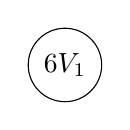
\begin{tikzpicture}[baseline=-0.4em]
\node[draw,circle] (4,0) {\zihao{6}$ V_{1} $};
\end{tikzpicture}
}
{量程为$ 2\ V $、内阻大约为$ 2 \ k\Omega $的电压表
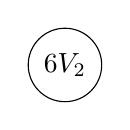
\begin{tikzpicture}[baseline=-0.4em]
\node[draw,circle] (4,0) {\zihao{6}$ V_{2} $};
\end{tikzpicture}
}
{量程为$ 3\ V $、内阻为$ 3 \ k\Omega $的电压表
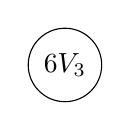
\begin{tikzpicture}[baseline=-0.4em]
\node[draw,circle] (4,0) {\zihao{6}$ V_{3} $};
\end{tikzpicture}
}

选择电压表 \tk{C} 
串联 \tk{6} 
$ k \Omega $的电阻可以改装成量程为$ 9\ V $的电压表。 

②利用一个电阻箱、一只开关、若干导线和改装好的电压表(此表用符号
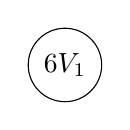
\begin{tikzpicture}[baseline=-0.4em]
\node[draw,circle] (4,0) {\zihao{6}$ V_{1} $};
\end{tikzpicture}
、
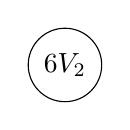
\begin{tikzpicture}[baseline=-0.4em]
\node[draw,circle] (4,0) {\zihao{6}$ V_{2} $};
\end{tikzpicture}
或
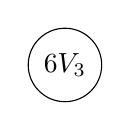
\begin{tikzpicture}[baseline=-0.4em]
\node[draw,circle] (4,0) {\zihao{6}$ V_{3} $};
\end{tikzpicture}
与一个电阻串联来表示,且可视为理想电压表),在虚线框内画出测量电源电动势及内阻的实验原理电路图。
\begin{figure}[h!]
\centering
\includesvg[width=0.23\linewidth]{picture/svg/701}
\end{figure}



③根据以上实验原理电路图进行实验,读出电压表示数为$ 1.50V $时、电阻箱的阻值为$ 15.0 \ \Omega $,电压表示数为$ 2.00V $时,电阻箱的阻值为$ 40.0 \ \Omega $,则电源的电动势$ E= $ \tk{7.5} 
$ V $、内阻$ r= $ \tk{10} 
$ \Omega $。 


\banswer{
②实验原理电路图如图示。
\includesvg[width=0.23\linewidth]{picture/svg/702} 
}


\newpage

\item 
\exwhere{$ 2012 $年理综四川卷}
某学习小组的同学拟探究小灯泡$ L $的伏安特性曲线,可供选用的器材如下:

小灯泡$ L $,规格“$ 4.0V $.$ 0.7A $”;

电流表$ A_{1} $,量程$ 3A $,内阻约为$ 0.1 \ \Omega $; 

电流表$ A_{2} $,量程$ 0.6A $,内阻$ r_{2} =0.2 \ \Omega $;

电压表$ V $,量程$ 3V $,内阻$ rV=9 \ k\Omega $; 

标准电阻$ R_{1} $,阻值$ 1 \ \Omega $;

标准电阻$ R_{2} $,阻值$ 3 $ $ k \Omega $;

滑动变阻器$ R $,阻值范围$ 0 \sim $ $ 10 \ \Omega $;

学生电源$ E $,电动势$ 6V $,内阻不计;

开关$ S $及导线若干。

①甲同学设计了如图$ 1 $所示的电路来进行测量,当通过$ L $的电流为$ 0.46\ A $时,电压表的示数如图$ 2 $所示,此时$ L $的电阻为 \tk{5} 
$ \Omega $。
\begin{figure}[h!]
\centering
\includesvg[width=0.2\linewidth]{picture/svg/696} \qquad \includesvg[width=0.2\linewidth]{picture/svg/697} \qquad \includesvg[width=0.2\linewidth]{picture/svg/698} \qquad \includesvg[width=0.2\linewidth]{picture/svg/699} 
\end{figure}

②乙同学又设计了如图$ 3 $所示的电路来进行测量,电压表指针指在最大刻度时,加在$ L $上的电压值是 \tk{4} 
$ V $。

③学习小组认为要想更准确地描绘出$ L $完整的伏安特性曲线,需要重新设计电路。请你在乙同学的基础上利用所供器材,在图$ 4 $所示的虚线框内补画出实验电路图,并在图上标明所选器材代号。


\banswer{
③由于电压表量程太小,所以需要改装,将它与$ R_{2} $串联即成为一个量程为$ 4.0V $的新的电压表;电流表$ A_{1} $量程太大,不可用,可以将$ A_{2} $改装:将它并联一个小电阻$ R_{1} $则成为一个量程为$ 0.72A $的新的电流表了。由于灯泡的电阻远小于电压表内阻而与电流表内阻相差不多,属于小电阻,故用电流表外接法比较合适。答案如答图$ 1 $较合适,若用答图$ 2 $则不太合适。

 \includesvg[width=0.4\linewidth]{picture/svg/700} 
 
说明:画出答图$ 1 $给$ 4 $分,只画出答图$ 2 $给$ 2 $分。
}




\newpage
\item
\exwhere{$ 2012 $年理综福建卷}
某研究性学习小组欲测定一块电池的电动势$ E $。

①先直接用多用电表测定该电池电动势。在操作无误的情况下,多用电表表盘示数如图,其示数为 \tk{9.4} 
$ V $。
\begin{figure}[h!]
\centering
\includesvg[width=0.23\linewidth]{picture/svg/703}
\end{figure}

②然后,用电压表$ V $、电阻箱$ R $、定值电阻$ R_{0} $、开关$ S $、若干导线和该电池组成电路,测定该电池电动势。
\begin{figure}[h!]
\centering
\includesvg[width=0.83\linewidth]{picture/svg/704}\\
 \begin{tabular}{|c|c|c|c|c|c|c|}
\hline 
R ($ \Omega $) & 166.7 & 71.4 & 50.0 & 33.3 & 25.0 & 20.0
\\
\hline
U (V) & 8.3 & 5.9 & 4.8 & 4.2 & 3.2 & 2.9
\\
\hline
$1/R
( \times 10^{-2} \Omega ^{-1}) $ & 0.60 & 1.40 & 2.00 & 3.00 & 4.00 & 5.00
\\
\hline
$ 1/U(V^{0} ) $ & 0.12 & 0.17 & 0.21 & 0.24 & 0.31 & 0.35\\ 
\hline 
\end{tabular}
\end{figure}




\begin{enumerate}
\renewcommand{\labelenumi}{\arabic{enumi}.}
% A(\Alph) a(\alph) I(\Roman) i(\roman) 1(\arabic)
%设定全局标号series=example	%引用全局变量resume=example
%[topsep=-0.3em,parsep=-0.3em,itemsep=-0.3em,partopsep=-0.3em]
%可使用leftmargin调整列表环境左边的空白长度 [leftmargin=0em]
\item
根据电路图,用笔画线代替导线,将实物图连接成完整电路。
\item 
闭合开关$ S $,调整电阻箱阻值$ R $,读出电压表$ V $相应示数$ U $。该学习小组测出大量数据,分析筛选出下表所示的$ R $、$ U $数据,并计算出相应的$ 1/R $与$ 1/U $的值。请用表中数据在坐标纸上描点,并作出$ 1/U-1/R $图线。

\item 
从图线中可以求得电动势$ E=$ \tk{$ 9.5-11.1 $} 
$V $	

\end{enumerate}


\banswer{
(ⅰ)连接电路如图所示。
(ⅱ)所作图象如图所示
 \includesvg[width=0.23\linewidth]{picture/svg/705} 
}



\newpage
\item 
\exwhere{$ 2018 $年江苏卷}
一同学测量某干电池的电动势和内阻。

\begin{enumerate}
\renewcommand{\labelenumi}{\arabic{enumi}.}
% A(\Alph) a(\alph) I(\Roman) i(\roman) 1(\arabic)
%设定全局标号series=example	%引用全局变量resume=example
%[topsep=-0.3em,parsep=-0.3em,itemsep=-0.3em,partopsep=-0.3em]
%可使用leftmargin调整列表环境左边的空白长度 [leftmargin=0em]
\item
如图所示是该同学正准备接入最后一根导线(图中虚线所示)时的实验电路。请指出图中在器材操作上存在的两个不妥之处。
\begin{figure}[h!]
\centering
\includesvg[width=0.23\linewidth]{picture/svg/706}
\end{figure}

 \tk{①开关未断开 ②电阻箱阻值为零}\hfullline 


\item 
实验测得的电阻箱阻值$ R $和电流表示数 $ I $ ,以及计算的$ \frac{1}{I} $数据见下表:
\begin{table}[h!]
\centering 
\begin{tabular}{|c|c|c|c|c|c|}
\hline 
R/$ \Omega $ & 8.0 & 7.0 & 6.0 & 5.0 & 4.0
\\
\hline
I/A & 0.15 & 0.17 & 0.19 & 0.22 & 0.26
\\
\hline
$ \frac{1}{I}/A^{–1} $ & 6.7 & 6.0 & 5.3 & 4.5 & 3.8\\ 
\hline 
\end{tabular}
\end{table} 

根据表中数据,在答题卡的方格纸上作出$R - \frac { 1 } { I }$关系图象。由图象可计算出该干电池的电动势为 \tk{$ 1.4 $($ 1.30 \sim 1.44 $都算对)} 
$ V $;内阻为 \tk{$ 1.2 $($ 1.0 \sim 1.4 $都算对)} 
$ \Omega $。
\begin{figure}[h!]
\centering
\includesvg[width=0.53\linewidth]{picture/svg/707}
\end{figure}


\item 
为了得到更准确的测量结果,在测出上述数据后,该同学将一只量程为$ 100 $ $ mV $的电压表并联在电流表的两端。调节电阻箱,当电流表的示数为$ 0.33 $ $ A $时,电压表的指针位置如图$ 2 $所示,则该干电池的电动势应为 \tk{$ 1.4 $(结果与($ 2 $)问第一个空格一致)} 
$ V $;内阻应为 \tk{$ 1.0 $(结果比($ 2 $)问第二个空格小$ 0.2 $)} 
$ \Omega $。



\end{enumerate}


\banswer{
($ 2 $)(见下图) :
 \includesvg[width=0.23\linewidth]{picture/svg/708} 
}


\newpage
\item 
\exwhere{$ 2014 $年理综新课标\lmd{1}卷}
利用如图$ (a) $所示电路,可以测量电源的电动势和内阻,所用的实验器材有:
待测电源,电阻箱$ R $(最大阻值$ 999.9 $ $ \Omega ) $,电阻$ R_{0} $(阻值为$ 3.0 $ $ \Omega ) $,电阻$ R_{1} $(阻值为$ 3.0 $ $ \Omega ) $,电流表$ A $(量程为$ 200 $ $ m{A} $,内阻为$ R_{A} =6.0 $ $ \Omega ) $,开关$ S $. 
\begin{figure}[h!]
\centering
\includesvg[width=0.23\linewidth]{picture/svg/709} \qquad 
 \includesvg[width=0.23\linewidth]{picture/svg/710} \qquad 
 \includesvg[width=0.23\linewidth]{picture/svg/711} 
\end{figure}



实验步骤如下:

①将电阻箱阻值调到最大,闭合开关$ S $;

②多次调节电阻箱,记下电流表的示数$ I $ 和电阻值箱相应的阻值$ R $;

③以$ \frac{1}{I} $为纵坐标,$ R $为横坐标,作 ­$\frac { 1 } { I } - R$ 图线(用直线拟合);

④求出直线的斜率$ k $和在纵轴上的截距$ b $. 为 \underlinegap .

回答下列问题:
\begin{enumerate}
\renewcommand{\labelenumii}{(\arabic{enumii})}
\item 
分别用$ E $和$ r $表示电源的电动势和内阻,则 与$ R $的关系式为$\frac { 1 } { I } = \frac { R _ { A } + R _ { 1 } } { E R _ { 1 } } R + \frac { 1 } { E } \left[ R _ { A } + \frac { R _ { A } + R _ { 1 } } { R _ { 1 } } \left( R _ { 0 } + r \right) \right]$.


\item 
实验得到的部分数据如下表所示,其中电阻$ R=3.0 $ $ \Omega $时电流表的示数如图$ (b) $所示,读出数据,完成下表.答:① \tk{0.110} 
,② \tk{9.09} 
.
\begin{table}[h!]
\centering 
\begin{tabular}{|c|c|c|c|c|c|c|c|}
\hline 
R/$ \Omega $ & 1.0 & 2.0 & 3.0 & 4.0 & 5.0 & 6.0 & 7.0
\\
\hline
I/A & 0.143 & 0.125 & ① & 0.100 & 0.091 & 0.084 & 0.077
\\
\hline
$ I^{-1}/A^{-1} $ & 6.99 & 8.00 & ② & 10.0 & 11.0 & 11.9 & 13.0\\ 
\hline 
\end{tabular}
\end{table} 


\item 
在图$ (c) $的坐标纸上将所缺数据点补充完整并作图,根据图线求得斜率$ k= $ \tk{1.0(在$ 0.961.04 $之间均给分) } 
$A^{-1} \Omega^{ -1} $,截距$ b= $ \tk{6.0(在$ 5.9\sim 6.1 $之间均给分)} 
$A^{-1} $.


\item 
根据图线求得电源电动势$ E=$ \tk{3.0 V (在$ 2.7\sim 3.3 $之间均给分)} 
$V $,内阻$ r= $ \tk{$1.0 \ \Omega $(在$ 0.6\sim 1.4 $之间均给分)} 
$\Omega $. 

\end{enumerate}

\banswer{
(3)图线如答图 
 \includesvg[width=0.23\linewidth]{picture/svg/712} 
}


\newpage
\item 
\exwhere{$ 2014 $年理综大纲卷}
现要测量某电源的电动势和内阻。可利用的器材有:电流表 \ammetermytikz ,内阻为$ 1.00 \ \Omega $;电压表 \voltmetermytikz ;阻值未知的定值电阻$ R_{1} $、$ R_{2} $、$ R_{3} $、$ R_{4} $、$ R_{5} $;开关$ S $;一端连有鳄鱼夹$ P $的导线$ 1 $,其他导线若干。某同学设计的测量电路如图$ (a) $所示。
\begin{figure}[h!]
\centering
\includesvg[width=0.83\linewidth]{picture/svg/713}
\end{figure}



\begin{enumerate}
\renewcommand{\labelenumi}{\arabic{enumi}.}
% A(\Alph) a(\alph) I(\Roman) i(\roman) 1(\arabic)
%设定全局标号series=example	%引用全局变量resume=example
%[topsep=-0.3em,parsep=-0.3em,itemsep=-0.3em,partopsep=-0.3em]
%可使用leftmargin调整列表环境左边的空白长度 [leftmargin=0em]
\item
按图 $ (a) $在实物图$ (b) $中画出连线,并标出导线$ 1 $和其$ P $端。
\item 
测量时,改变鳄鱼夹$ P $所夹的位置,使$ R_{1} $、$ R_{2} $、$ R_{3} $、$ R_{4} $、$ R_{5} $依次串入电路,记录对应的电压表的示数$ U $和电流表的示数 \lmd{1} 。 数据如下表所示。根据表中数据,在图($ c $)中的坐标纸上将所缺数据点补充完整,并画出$ U-I $图线。

\begin{figure}[h!]
\centering 
\begin{tabular}{|c|c|c|c|c|c|}
\hline 
I(mA) & 193 & 153 & 111 & 69 & 30
 \\
\hline
U(V) & 2.51 & 2.59 & 2.68 & 2.76 & 2.84\\ 
\hline 
\end{tabular} \qquad 
\includesvg[width=0.35\linewidth]{picture/svg/714} 
\end{figure}


\item 
根据$ U-I $图线求出电源的电动势$ E= $ \tk{$ 2.90 $(在$ 2.89 \sim 2.91 $之间均给分)} 
$ V $,内阻$ r= $ \tk{$ 1.02 $(在$ 0.93 \sim 1.13 $之间均给分)} 
$ \Omega $。




\end{enumerate}

\banswer{
$ (1) $连接如答图$ 1 $所示.$ U $­ \lmd{1} 图线如答图$ 2 $所示.

 \includesvg[width=0.23\linewidth]{picture/svg/715} 
}



\newpage
\item 
\exwhere{$ 2014 $年理综北京卷}
利用电流表和电压表测定一节干电池的电动势和内电阻。要求尽量减小实验误差。
\begin{enumerate}
\renewcommand{\labelenumi}{\arabic{enumi}.}
% A(\Alph) a(\alph) I(\Roman) i(\roman) 1(\arabic)
%设定全局标号series=example	%引用全局变量resume=example
%[topsep=-0.3em,parsep=-0.3em,itemsep=-0.3em,partopsep=-0.3em]
%可使用leftmargin调整列表环境左边的空白长度 [leftmargin=0em]
\item
应该选择的实验电路是图$ 1 $中的 \tk{甲} 
(选项“甲”或“乙”)。
\begin{figure}[h!]
\centering
\includesvg[width=0.37\linewidth]{picture/svg/716}
\end{figure}

\item 
现有电流表($ 0\sim 0.6\ A $)、开关和导线若干,以及以下器材:
\fourchoices
{电压表($ 015V $)}
{电压表($ 03V $)}
{滑动变阻器($ 050 \ \Omega $)}
{滑动变阻器($ 0500 \ \Omega $)}

实验中电压表应选用 \tk{B} 
;滑动变阻器应选用 \tk{C} 
;(选填相应器材前的字母)
\item 
某位同学记录的$ 6 $组数据如下表所示,其中$ 5 $组数据的对应点已经标在图$ 2 $的坐标纸上,请标出余下一组数据的对应点,并画出 $ U-I $ 图线。
\begin{table}[h!]
\centering 
\begin{tabular}{|c|c|c|c|c|c|c|}
\hline 
序号 & 1 & 2 & 3 & 4 & 5 & 6
 \\
\hline
电压U(V) & 1.45 & 1.40 & 1.30 & 1.25 & 1.20 & 1.10
 \\
\hline
电流I( A ) & 0.060 & 0.120 & 0.240 & 0.260 & 0.360 & 0.480\\ 
\hline 
\end{tabular} \qquad 
\includesvg[width=0.23\linewidth]{picture/svg/718} 
\end{table} 


\item 
根据($ 3 $)中所画图线可得出干电池的电动势$ E= $ \tk{1.50} 
$ V $,内电阻$ r= $ \tk{0.83} 
$ \Omega $
\item 
实验中,随着滑动变阻器滑片的移动,电压表的示数$ U $以及干电池的输出功率$ P $都会发生变化,图$ 3 $的各示意图中正确反映$ P-U $关系的是 \tk{C} 
。
\begin{figure}[h!]
\centering
\includesvg[width=0.83\linewidth]{picture/svg/717}
\end{figure}





\end{enumerate}


\banswer{
$ (3) $第$ 3 $个点为数据误差,连线时略过,如图:
 \includesvg[width=0.23\linewidth]{picture/svg/719} 
}














\newpage
\item 
\exwhere{$ 2014 $年物理上海卷}
在“用$ DIS $测电源的电动势和内阻”的实验中:
\begin{figure}[h!]
\centering
\includesvg[width=0.73\linewidth]{picture/svg/720}
\end{figure}

\begin{enumerate}
\renewcommand{\labelenumii}{(\arabic{enumii})}

\item 
将待测电池组、滑动变阻器、电流传感器、电压传感器、定值电阻、电键及若干导线连接成电路如图$ (a) $所示。图中未接导线的$ A $端应接在 \tk{C} 
点(选填$ : $ “$ B $”、“$ C $”、“$ D $”或“$ E $”)。


\item 
实验得到的$ U-I $关系如图$ (b) $中的直线$ 1 $所示,则电池组的电动势为 \tk{2.8} 
$ V $,内电阻阻值为 \tk{2} $ \Omega $ 
。


\item 
为了测量定值电阻的阻值,应在图$ (a) $中将“$ A $”端重新连接到 \tk{D} 
点(选填$ : $ “$ B $”、“$ C $”、“$ D $”或“$ E $”),所得到的$ U-I $关系如图$ (b) $中的直线$ \lmd{2} $所示,则定值电阻的阻值为 \tk{3} $ \Omega $
。

\end{enumerate}


\item 
\exwhere{$ 2015 $年江苏卷}
小明利用如图$ 1 $所示的实验装置测量一干电池的电动势和内阻.
\begin{figure}[h!]
\centering
\includesvg[width=0.83\linewidth]{picture/svg/725}
\end{figure}

\begin{enumerate}
\renewcommand{\labelenumii}{(\arabic{enumii})}
\item 
题 $ 1 $ 图中电流表的示数为 \tk{0.44} 
A.


\item 
调节滑动变阻器,电压表和电流表的示数记录如下:
\begin{table}[h!]
\centering 
\begin{tabular}{|c|c|c|c|c|c|}
\hline 
U(V) & 1.45 & 1.36 & 1.27 & 1.16 & 1.06
 \\
\hline
I(A) & 0.12 & 0.20 & 0.28 & 0.36 & 0.44\\ 
\hline 
\end{tabular}
\end{table} 



请根据表中的数据,在答题卡的方格纸上作出 $ U-I $ 图线.

由图线求得:电动势 $ E = $ \tk{ $ 1.60 $ $ (1 $. $ 58 $ $ \sim $ $ 1 $. $ 62 $ 都算对)} 
$ V $;内阻 $ r = $ \tk{$ 1. 20 $ $ (1 $. $ 18 $ $ \sim $ $ 1 $. $ 26 $ 都算对)} 
$ \Omega $.


\item 
实验时,小明进行了多次测量,花费了较长时间,测量期间一直保持电路闭合。 其实,从实验误差考虑,这样的操作不妥,因为 \tk{干电池长时间使用后,电动势和内阻会发生变化,导致实验误差增大。 } 
。




\end{enumerate}


\banswer{
(2) $ U-I $ 图线见右图 :
\includesvg[width=0.23\linewidth]{picture/svg/726} 
}


\newpage

\item 
\exwhere{$ 2014 $年理综福建卷}
某研究性学习小组利用伏安法测定某一电池组的电动势和内阻,实验原理如图甲所示,其中,虚线框内为用灵敏电流计$ G $改装的电流表$ A $,$ V $为标准电压表,$ E $为待测电池组,$ S $为开关,$ R $为滑动变阻器,$ R_{0} $是标称值为$ 4.0 \ \Omega $的定值电阻。
\begin{figure}[h!]
\centering
\includesvg[width=0.63\linewidth]{picture/svg/721}
\end{figure}


①已知灵敏电流计$ G $的满偏电流$ I_{g} =100 \ \mu A $、内阻$ r_g=2.0 \ k\Omega $,若要改装后的电流表满偏电流为$ 200 \ mA $,应并联一只 \tk{1.0} 
$ \Omega $(保留一位小数)的定值电阻$ R_{1} $;

②根据图甲,用笔画线代替导线将图乙连接成完整电路;

③某次实验的数据如下表所示:

\begin{table}[h!]
\centering 
\begin{tabular}{|c|c|c|c|c|c|c|c|c|}
\hline 
测量次数 & 1 & 2 & 3 & 4 & 5 & 6 & 7 & 8
 \\
\hline
电压表V读数U/V & 5.26 & 5.16 & 5.04 & 4.94 & 4.83 & 4.71 & 4.59 & 4.46
 \\
\hline
改装表A读数I/mA & 20 & 40 & 60 & 80 & 100 & 120 & 140 & 160\\ 
\hline 
\end{tabular}
\end{table} 

该小组借鉴“研究匀变速直线运动”实验中计算加速度的方法(逐差法),计算出电池组的内阻 
$ r= $ \tk{$ 1.66 $} 
$ \Omega $(保留两位小数);为减小偶然误差,逐差法在数据处理方面体现出的主要优点是 \tk{充分利用测得的数据 } 
。


④该小组在前面实验的基础上,为探究图甲电路中各元器件的实际阻值对测量结果的影响,用一已知电动势和内阻的标准电池组,通过上述方法多次测量后发现:电动势的测量值与已知值几乎相同,但内阻的测量值总是偏大。若测量过程无误,则内阻测量值总是偏大的原因是 \tk{CD} 
。(填选项前的字母)
\fourchoices
{电压表内阻的影响 }
{滑动变阻器的最大阻值偏小}
{$ R_{1} $的实际阻值比计算值偏小}
{$ R_{0} $的实际阻值比标称值偏大}


\banswer{
②如答图所示:
 \includesvg[width=0.23\linewidth]{picture/svg/722} 
}

\newpage
\item 
\exwhere{$ 2015 $年理综天津卷}
用电流表和电压表测定由三节干电池串联组成的电池组(电动势约为$ 4.5V $,内电阻约为$ 1 \ \Omega $)的电动势和内电阻,除了待测电池组,电建,导线外,还有下列器材供选用:

$ A $电流表:量程$ 0.6A $,内电阻约$ 1 \ \Omega $

$ B $电流表:量程$ 3A $,内电阻约为$ 0.2 \ \Omega $

$ C $电压表:量程$ 3V $,内电阻约为$ 30 \ k\Omega $

$ D $电压表:量程$ 6V $,内电阻约为$ 60 \ k\Omega $

$ E $滑动变阻器:$ 0-1000 \ \Omega $,额定电流$ 0.5\ A $

$ F $滑动变阻器:$ 0-20 \ \Omega $,额定电流$ 2\ A $

①为了使测量结果尽量准确,电流表应选用 \tk{A} 
,电压表应选用 \tk{D} 
,滑动变阻器应选用 \tk{F} 
(均填仪器的字母代号)

②右图为正确选择仪器后,连好的部分电路,为了使测量误差尽量小,还需在电路中用导线将 \tk{a} 
和 \tk{d} 
相连、 \tk{C} 
和 \tk{g} 
相连、 \tk{f} 
和 \tk{h} 
相连(均填仪器上接线柱的字母代号)
\begin{figure}[h!]
\centering
\includesvg[width=0.43\linewidth]{picture/svg/723}
\end{figure}

③实验时发现电流表坏了,于是不再使用电流表,剩余仪器中仅用电阻箱替换掉滑动变阻器,重新连接电路,仍能完成实验,实验中读出几组电阻箱的阻值$ R $和对应电压表的示数$ U $;用图像法处理采集到数据,为在直角坐标系中得到的函数图像是一条直线,则可以 \tk{$ \frac{1}{U} $、$ \dfrac{1}{R} $、$ U $} 
为纵坐标,以 \tk{$ \frac{U}{R} $、$ \frac{R}{U} $、$ R $} 
为横坐标.

\banswer{
②为减小误差,电流表应采用内接法,同时注意电表的正、负接线柱,电路图如右图示,故可知导线应连接$ a $ $ d $ 、$ c $ $ g $、 $ f $ $ h $。
 \includesvg[width=0.23\linewidth]{picture/svg/724} 
}








\newpage
\item 
\exwhere{$ 2015 $年理综安徽卷}
某同学为了测量一节电池的电动势和内阻,从实验室找到以下器材:一个满偏电流为$ 100 $ $ \mu A $,内阻为$ 2500 $ $ \Omega $的表头,一个开关,两个电阻箱($ 0 - 999.9 $ $ \Omega $)和若干导线。
\begin{enumerate}
\renewcommand{\labelenumi}{\arabic{enumi}.}
% A(\Alph) a(\alph) I(\Roman) i(\roman) 1(\arabic)
%设定全局标号series=example	%引用全局变量resume=example
%[topsep=-0.3em,parsep=-0.3em,itemsep=-0.3em,partopsep=-0.3em]
%可使用leftmargin调整列表环境左边的空白长度 [leftmargin=0em]
\item
由于表头量程偏小,该同学首先需将表头改装成量程为$ 50 $ $ m_{A} $的电流表,则应将表头与电阻箱 \tk{并联} 
(填“串联”或“并联”),并将该电阻箱阻值调为 \tk{5.0} 
$ \Omega $。

\item 
接着该同学用改装的电流表对电池的电动势及内阻进行测量,实验电路如图$ 1 $所示,通过改变电阻$ R $测相应的电流 \lmd{1} ,且作相关计算后一并记录如下表。
\begin{figure}[h!]
\centering
\includesvg[width=0.23\linewidth]{picture/svg/727}
\end{figure}

\begin{table}[h!]
\centering 
\begin{tabular}{|c|c|c|c|c|c|c|}
\hline 
& 1 & 2 & 3 & 4 & 5 & 6
 \\
\hline
R($ \Omega $) & 95.0 & 75.0 & 55.0 & 45.0 & 35.0 & 25.0
 \\
\hline
I(mA) & 15.0 & 18.7 & 24.8 & 29.5 & 36.0 & 48.0
 \\
\hline
IR(V) & 1.42 & 1.40 & 1.36 & 1.33 & 1.26 & 1.20\\ 
\hline 
\end{tabular} \qquad 
\includesvg[width=0.23\linewidth]{picture/svg/728} 
\end{table} 



①根据表中数据,图$ 2 $中已描绘出四个点,请将第$ 5 $、$ 6 $两组数据也描绘在图$ 2 $中,并画$ IR-I $ 图线.

②根据图线可得电池的电动势$ E $是 \tk{1.53} 
$ V $,内阻$ r $是 \tk{2} 
$ \Omega $。




\end{enumerate}

\banswer{
($ 2 $)①倾斜直线如下图示;
 \includesvg[width=0.23\linewidth]{picture/svg/729} 
}


\newpage

\item 
\exwhere{$ 2017 $年天津卷}
某探究性学习小组利用如图所示的电路测量电池的电动势和内阻。其中电流表$ A_{1} $的内阻$ r_{1} =1.0 $ $ k \Omega $,电阻$ R_{1} =9.0 $ $ k \Omega $,为了方便读数和作图,给电池串联一个$ R_{0} =3.0 $ $ \Omega $的电阻。
\begin{figure}[h!]
\centering
\includesvg[width=0.23\linewidth]{picture/svg/730} \qquad 
\includesvg[width=0.23\linewidth]{picture/svg/731} 
\end{figure}


①按图示电路进行连接后,发现$ aa ^{\prime} $、$ bb ^{\prime} $和$ cc ^{\prime} $三条导线中,混进了一条内部断开的导线。为了确定哪一条导线内部是断开的,将电键$ S $闭合,用多用电表的电压挡先测量,$ a $、$ b ^{\prime} $间电压,读数不为零,再测量$ a $、$ a ^{\prime} $间电压,若读数不为零,则一定是 \tk{$ aa ^{\prime} $} 
导线断开;若读数为零,则一定是 \tk{$ bb ^{\prime} $} 
导线断开。

②排除故障后,该小组顺利完成实验。通过多次改变滑动变阻器触头位置,得到电流表$ A_{1} $和$ A_{2} $的多组$ I_{1} $、$ I_{2} $数据,作出图象如右图。由$ I_{1} - I_{2} $图象得到的电池的电动势$ E=$ \tk{$ 1.41 $($ 1.36 \sim 1.44 $均可)} 
$V $,内阻$ r= $ \tk{,$ 0.5 $($ 0.4 \sim 0.6 $均可)} 
$ \Omega $。








\end{enumerate}



\bta{练习使用多用表}



\begin{enumerate}
%\renewcommand{\labelenumi}{\arabic{enumi}.}
% A(\Alph) a(\alph) I(\Roman) i(\roman) 1(\arabic)
%设定全局标号series=example	%引用全局变量resume=example
%[topsep=-0.3em,parsep=-0.3em,itemsep=-0.3em,partopsep=-0.3em]
%可使用leftmargin调整列表环境左边的空白长度 [leftmargin=0em]
\item
\exwhere{$ 2019 $ 年物理全国\lmd{3}卷}
某同学欲将内阻为 $ 98.5 \ \Omega $、量程为 $ 100 \ uA $ 的电流表改装成欧姆表并进行刻
度和校准,要求改装后欧姆表的 $ 15 \ k\Omega $刻度正好对应电流表表盘的 $ 50 \ uA $ 刻度。可选用的器材还有:
定值电阻 $ R_{0} $(阻值 $ 14 \ k\Omega $),滑动变阻器 $ R_{1} $(最大阻值 $ 1500 \ \Omega $),滑动变阻器 $ R_{2} $(最大阻值 $ 500 \ \Omega $),
电阻箱($ 0 \sim 99999.9 \ \Omega $),干电池($ E=1.5 \ V $,$ r=1.5 \ \Omega $),红、黑表笔和导线若干。
\begin{figure}[h!]
\centering
\begin{subfigure}{0.4\linewidth}
\centering
\includesvg[width=0.7\linewidth]{picture/svg/GZ-3-tiyou-0990} 
\caption{}\label{}
\end{subfigure}
\begin{subfigure}{0.4\linewidth}
\centering
\includesvg[width=0.7\linewidth]{picture/svg/GZ-3-tiyou-0991} 
\caption{}\label{}
\end{subfigure}
\begin{subfigure}{0.4\linewidth}
\centering
\includesvg[width=0.7\linewidth]{picture/svg/GZ-3-tiyou-0992} 
\caption{}\label{}
\end{subfigure}
\end{figure}


\begin{enumerate}
%\renewcommand{\labelenumi}{\arabic{enumi}.}
% A(\Alph) a(\alph) I(\Roman) i(\roman) 1(\arabic)
%设定全局标号series=example	%引用全局变量resume=example
%[topsep=-0.3em,parsep=-0.3em,itemsep=-0.3em,partopsep=-0.3em]
%可使用leftmargin调整列表环境左边的空白长度 [leftmargin=0em]
\item
欧姆表设计

将图($ a $)中的实物连线组成欧姆表。
欧姆表改装好后,滑动变阻器 $ R $ 接入电路的电
阻应为 \underlinegap $ \Omega $:滑动变阻器选 \underlinegap (填“$ R_{1} $”或“$ R_{2} $”)。



\item 
刻度欧姆表表盘

通过计算,对整个表盘进行电阻刻度,如图($ b $)所示。表盘上 $ a $、$ b $ 处的电流刻度分别为 $ 25 $ 和 $ 75 $,
则 $ a $、$ b $ 处的电阻刻度分别为 \underlinegap 、 \underlinegap 。


\item 
校准

红、黑表笔短接,调节滑动变阻器,使欧姆表指针指向 \underlinegap $ k \Omega $处;将红、黑表笔与电阻箱连接,记
录多组电阻箱接入电路的电阻值及欧姆表上对应的测量值,完成校准数据测量。若校准某刻度时,
电阻箱旋钮位置如图($ c $)所示,则电阻箱接入的阻值为 \underlinegap $ \Omega $。




\end{enumerate}


\tk{
\begin{enumerate}
%\renewcommand{\labelenumi}{\arabic{enumi}.}
% A(\Alph) a(\alph) I(\Roman) i(\roman) 1(\arabic)
%设定全局标号series=example	%引用全局变量resume=example
%[topsep=-0.3em,parsep=-0.3em,itemsep=-0.3em,partopsep=-0.3em]
%可使用leftmargin调整列表环境左边的空白长度 [leftmargin=0em]
\item
$ 900 $ \quad $ R_{1} $
连线如图:
\begin{center}
\includesvg[width=0.23\linewidth]{picture/svg/GZ-3-tiyou-0993} 	
\end{center}
\item 	
$ 45 $ \quad $ 5 $
\item 	
$ 0 $ \quad $ 35000.0 $
\end{enumerate}
} 

\item 
\exwhere{$ 2011 $ 年理综北京卷}
用如图 $ 1 $ 所示的多用电表测量电阻,要用到选择开关 $ K $ 和两个部件 $ S $、$ T $。请根据下列步骤完成电
阻测量:

①旋动部件 \underlinegap ,使指针对准电流的“$ 0 $”刻线。

②将 $ K $ 旋转到电阻挡“$ \times 10^{0} $”的位置。



③将插入“$ + $”、“$ - $”插孔的表笔短接,旋动部件 \underlinegap ,使指针对准
电阻的 \underlinegap (填“$ 0 $ 刻线”或“$ \infty $刻线”。


④将两表笔分别与待测电阻相接,发现指针偏转角度过小。为了得
到比较准确的测量结果,请从下列选项中挑出合理的步骤,并按 \underlinegap 
的顺序进行操作,再完成读数测量。
\begin{figure}[h!]
\centering
\includesvg[width=0.23\linewidth]{picture/svg/GZ-3-tiyou-0994}
\end{figure}


\fourchoices
{将 $ K $ 旋转到电阻挡“$ \times 1k $”的位置}
{将 $ K $ 旋转到电阻挡“$ \times 10 $”的位置}
{将两表笔的金属部分分别与被测电阻的两根引线相接}
{将两表笔短接,旋动合适部件,对电表进行校准}







\item
\exwhere{$ 2011 $ 年理综重庆卷}
某电动机的三组线圈①、②、③阻值相同,均为几欧姆,接法可能是图 $ 1 $ 中甲、乙两种之
一,$ A $、$ B $ 和 $ C $ 是外接头。现有一组线圈断路,维修人员通
过多用电表测量外接头之间的电阻来判断故障,若测量 $ A $
和 $ B $ 之间、$ B $ 和 $ C $ 之间、$ A $ 和 $ C $ 之间的电阻时,多用电表
指针偏转分别如图 $ 2(a) $、$ (b) $、$ (c) $所示,则测量中使用的欧
姆档的倍率是 \underlinegap (填 $ \times 1 $、 $ \times 10 $、 $ \times 100 $ 或 $ \times 1k $ ),三组线圈的接法是 \underlinegap (填甲或乙),断路线圈是 \underlinegap (填①、②或③)。
\begin{figure}[h!]
\centering
\begin{subfigure}{0.4\linewidth}
\centering
\includesvg[width=0.7\linewidth]{picture/svg/GZ-3-tiyou-0995} 
\caption{}\label{}
\end{subfigure}
\begin{subfigure}{0.8\linewidth}
\centering
\includesvg[width=0.8\linewidth]{picture/svg/GZ-3-tiyou-0996} 
\caption{}\label{}
\end{subfigure}
\end{figure}


\tk{$ \times 1 $ \quad 乙 \quad ③} 


\item 
\exwhere{$ 2014 $ 年理综重庆卷}
某照明电路出现故障,其电路如图 $ 1 $ 所示,该电路用标称值 $ 12 \ V $ 的蓄电池为电源,导线及其接
触完好。维修人员使用已调好的多用表直流 $ 50 \ V $ 挡检测故障。他将黑表笔接在 $ c $ 点,用红表笔分别
探测电路的 $ a $、$ b $ 点。
\begin{figure}[h!]
\centering
\begin{subfigure}{0.4\linewidth}
\centering
\includesvg[width=0.7\linewidth]{picture/svg/GZ-3-tiyou-0997} 
\caption{}\label{}
\end{subfigure}
\begin{subfigure}{0.4\linewidth}
\centering
\includesvg[width=0.7\linewidth]{picture/svg/GZ-3-tiyou-0998} 
\caption{}\label{}
\end{subfigure}

\end{figure}

\begin{enumerate}
%\renewcommand{\labelenumi}{\arabic{enumi}.}
% A(\Alph) a(\alph) I(\Roman) i(\roman) 1(\arabic)
%设定全局标号series=example	%引用全局变量resume=example
%[topsep=-0.3em,parsep=-0.3em,itemsep=-0.3em,partopsep=-0.3em]
%可使用leftmargin调整列表环境左边的空白长度 [leftmargin=0em]
\item
断开开关,红表笔接 $ a $ 点时多用表指示如题图 $ 2 $ 所示,读数为 \underlinegap 
$ V $,说明 \underlinegap 
正常(选
填:蓄电池、保险丝、开关、小灯)。


\item 
红表笔接 $ b $ 点,断开开
关时,表针不偏转,闭合
开关后,多用表指示仍然
和题图 $ 2 $ 相同,可判断
发生故障的器件
是 \underlinegap 。(选填:蓄电池、保险丝、开关、小灯)


\end{enumerate}


\tk{
\begin{enumerate}
%\renewcommand{\labelenumi}{\arabic{enumi}.}
% A(\Alph) a(\alph) I(\Roman) i(\roman) 1(\arabic)
%设定全局标号series=example	%引用全局变量resume=example
%[topsep=-0.3em,parsep=-0.3em,itemsep=-0.3em,partopsep=-0.3em]
%可使用leftmargin调整列表环境左边的空白长度 [leftmargin=0em]
\item
$11.5 \quad(11.2 \sim 11.8)$;蓄电池
\item 
小灯
\end{enumerate}
} 

\item 
\exwhere{$ 2013 $ 年上海卷}
为确定某电子元件的电气特性,做如下测量。
\begin{figure}[h!]
\centering
\begin{subfigure}{0.4\linewidth}
\centering
\includesvg[width=0.7\linewidth]{picture/svg/GZ-3-tiyou-0999} 
\caption{}\label{}
\end{subfigure}
\begin{subfigure}{0.4\linewidth}
\centering
\includesvg[width=0.7\linewidth]{picture/svg/GZ-3-tiyou-1000} 
\caption{}\label{}
\end{subfigure}
\end{figure}

\begin{enumerate}
%\renewcommand{\labelenumi}{\arabic{enumi}.}
% A(\Alph) a(\alph) I(\Roman) i(\roman) 1(\arabic)
%设定全局标号series=example	%引用全局变量resume=example
%[topsep=-0.3em,parsep=-0.3em,itemsep=-0.3em,partopsep=-0.3em]
%可使用leftmargin调整列表环境左边的空白长度 [leftmargin=0em]
\item
用多用表测量该元件的电阻,选用“$ \times 100 $”倍率的电阻
档测量,发现多用表指针偏转过大,因此需选择 \underlinegap 0倍
率的电阻档(填:“$ \times 10 $”或“$ \times 1k $”),并 \underlinegap 再进行
测量,多用表的示数如图$ (a) $所示,测量结果
为 \underlinegap 
$ \Omega $。




\item 
将待测元件(额定电压 $ 9 \ V $)、蓄电池、滑动变阻器、
电流表、多用表、电键及若干导线连接成电路如图$ (b) $所
示。添加连线,使电路能测量该元件完整的伏安特性。



本实验中使用多用表测电压,多用表的选择开关应调到 \underlinegap 档(填:“直流电压 $ 10 \ V $”
或“直流电压 $ 50 \ V $”)。




\end{enumerate}

\tk{
\begin{enumerate}
%\renewcommand{\labelenumi}{\arabic{enumi}.}
% A(\Alph) a(\alph) I(\Roman) i(\roman) 1(\arabic)
%设定全局标号series=example	%引用全局变量resume=example
%[topsep=-0.3em,parsep=-0.3em,itemsep=-0.3em,partopsep=-0.3em]
%可使用leftmargin调整列表环境左边的空白长度 [leftmargin=0em]
\item
$ \times 10 $ \quad 欧姆调零 \quad $ 70 $
\item 
电路如图;直流电压 $ 10 \ V $ 档
\begin{center}
\includesvg[width=0.23\linewidth]{picture/svg/GZ-3-tiyou-1001} 
\end{center}
\end{enumerate}
} 

\item 
\exwhere{$ 2013 $ 年新课标 \lmd{1} 卷}
某学生实验小组利用图$ (a) $所示电路,测量多用电表内电池的电动势和电阻“$ \times 1k $”挡内部
电路的总电阻。使用的器材有:\\
多用电表;\\
电压表:量程 $ 5 \ V $,内阻十几千欧;\\
滑动变阻器:最大阻值 $ 5 \ k\Omega $;\\
导线若干。

回答下列问题:
\begin{figure}[h!]
\centering
\begin{subfigure}{0.4\linewidth}
\centering
\includesvg[width=0.7\linewidth]{picture/svg/GZ-3-tiyou-1002} 
\caption{}\label{}
\end{subfigure}
\begin{subfigure}{0.4\linewidth}
\centering
\includesvg[width=0.7\linewidth]{picture/svg/GZ-3-tiyou-1003} 
\caption{}\label{}
\end{subfigure}
\begin{subfigure}{0.4\linewidth}
\centering
\includesvg[width=0.7\linewidth]{picture/svg/GZ-3-tiyou-1004} 
\caption{}\label{}
\end{subfigure}
\begin{subfigure}{0.4\linewidth}
\centering
\includesvg[width=0.7\linewidth]{picture/svg/GZ-3-tiyou-1006} 
\caption{}\label{}
\end{subfigure}

\end{figure}

\begin{enumerate}
%\renewcommand{\labelenumi}{\arabic{enumi}.}
% A(\Alph) a(\alph) I(\Roman) i(\roman) 1(\arabic)
%设定全局标号series=example	%引用全局变量resume=example
%[topsep=-0.3em,parsep=-0.3em,itemsep=-0.3em,partopsep=-0.3em]
%可使用leftmargin调整列表环境左边的空白长度 [leftmargin=0em]
\item
将多用电表挡位调到电阻“$ \times 1k $”挡,再将红表笔和黑表
笔 \underlinegap ,调零点。


\item 
将图$ ((a) $中多用电表的红表笔和 \underlinegap 
(填“$ 1 $”或“$ 2 $)端相连,黑表笔连接另一端。


\item 
将滑动变阻器的滑片调到适当位置,使多角电表的示数如图$ (b) $所示,这时电压表的示数如图$ (c) $
所示。多用电表和电压表的读数分别为 \underlinegap $ k \Omega $和 \underlinegap $ V $。



\item 
调节滑动变阻器的滑片,使其接入电路的阻值为零。此时多用电表和
电压表的读数分别为 $ 12.0 \ k\Omega $和 $ 4.00 \ V $。从测量数据可知,电压表的内阻为 \underlinegap $ k \Omega $。




\item 
多用电表电阻挡内部电路可等效为由一个无内阻的电池、一个理想电流表和一个电阻串联而成的
电路,如图$ (d) $所示。根据前面的实验数据计算可得,此多用电表内电池的电动势为 \underlinegap $ V $,电
阻“$ \times 1k $”挡内部电路的总电阻为 \underlinegap $ k \Omega $。


\end{enumerate}

\tk{
\begin{enumerate}
%\renewcommand{\labelenumi}{\arabic{enumi}.}
% A(\Alph) a(\alph) I(\Roman) i(\roman) 1(\arabic)
%设定全局标号series=example	%引用全局变量resume=example
%[topsep=-0.3em,parsep=-0.3em,itemsep=-0.3em,partopsep=-0.3em]
%可使用leftmargin调整列表环境左边的空白长度 [leftmargin=0em]
\item
短接
\item 
$ 15.0 $ \quad $ 3.60 $
\item 
$ 12.0 $
\item 
$ 9.00 $ \quad $ 15.0 $
\end{enumerate}
} 






\item
\exwhere{$ 2012 $ 年江苏卷}
如图$ a $所示的黑箱中有三只完全相同的电学元件,小明使用多用电表对其进行探测。
\begin{figure}[h!]
\centering
\begin{subfigure}{0.4\linewidth}
\centering
\includesvg[width=0.7\linewidth]{picture/svg/GZ-3-tiyou-1007} 
\caption{}\label{}
\end{subfigure}
\begin{subfigure}{0.4\linewidth}
\centering
\includesvg[width=0.7\linewidth]{picture/svg/GZ-3-tiyou-1008} 
\caption{}\label{}
\end{subfigure}
\end{figure}
\begin{enumerate}
%\renewcommand{\labelenumi}{\arabic{enumi}.}
% A(\Alph) a(\alph) I(\Roman) i(\roman) 1(\arabic)
%设定全局标号series=example	%引用全局变量resume=example
%[topsep=-0.3em,parsep=-0.3em,itemsep=-0.3em,partopsep=-0.3em]
%可使用leftmargin调整列表环境左边的空白长度 [leftmargin=0em]
\item
在使用多用电表前,发现指针不在左边“$ 0 $”刻度线处,应先调整图$ b $中多用电表的 \underlinegap 
(选填“$ A $”、“$ B $”或“$ C $”)。

\item 
在用多用电表的直流电压挡探测黑箱 $ a $、$ b $ 接点间是否存在电源时,一表笔接 $ a $,另一表笔应
\underlinegap 
(选填“短暂”或“持续”)接 $ b $,同时观察指针偏转情况。

\item 
在判定黑箱中无电源后,将选择开关旋至“$ \times 1 $”挡,调节好多用电表,测量各接点间的阻值. 测量中发
现,每对接点间正反向阻值均相等,测量记录如下表. 两表笔分别接 $ a $、$ b $ 时,多用电表的示数如题图$ b $所示.请将记录表补充完整,并在答题卡的黑箱图中画出一种可能的电路.
\begin{table}[h!]
\centering 
\begin{tabular}{|c|c|}
\hline 
两表笔接的接点 & 多用电表的示数
\\
\hline
$ a $, $ b $ & $ \underlinegap \Omega $
\\
\hline
$ a $, $ c $ & $ 10.0 \ \Omega $
\\
\hline
$ b $, $ c $ & $ 15.0 \ \Omega $\\ 
\hline 
\end{tabular}
\hfil
\begin{tabular}{c}
\includesvg[width=0.3\linewidth]{picture/svg/GZ-3-tiyou-1009} 
\end{tabular}
\end{table} 




\end{enumerate}

\tk{
\begin{enumerate}
%\renewcommand{\labelenumi}{\arabic{enumi}.}
% A(\Alph) a(\alph) I(\Roman) i(\roman) 1(\arabic)
%设定全局标号series=example	%引用全局变量resume=example
%[topsep=-0.3em,parsep=-0.3em,itemsep=-0.3em,partopsep=-0.3em]
%可使用leftmargin调整列表环境左边的空白长度 [leftmargin=0em]
\item
$ A $
\item 
短暂
\item 
$ 5.0 \ \Omega $,可能的电路有两种,如图:
\begin{center}
\includesvg[width=0.23\linewidth]{picture/svg/GZ-3-tiyou-1010} 
\end{center}
\begin{center}
\includesvg[width=0.23\linewidth]{picture/svg/GZ-3-tiyou-1011} 
\end{center}
\end{enumerate}
} 


\item
\exwhere{$ 2012 $ 年物理上海卷}
在练习使用多用表的实验中:
\begin{enumerate}
%\renewcommand{\labelenumi}{\arabic{enumi}.}
% A(\Alph) a(\alph) I(\Roman) i(\roman) 1(\arabic)
%设定全局标号series=example	%引用全局变量resume=example
%[topsep=-0.3em,parsep=-0.3em,itemsep=-0.3em,partopsep=-0.3em]
%可使用leftmargin调整列表环境左边的空白长度 [leftmargin=0em]
\item
某同学连接的电路如图所示。
% TODO: \usepackage{graphicx} required
\begin{figure}[h!]
\centering
 %\includesvg[width=0.23\linewidth]{picture/svg/GZ-3-tiyou-1012} 
\includegraphics[width=0.5\linewidth]{picture/screenshot060}
\end{figure}

\begin{enumerate}
%\renewcommand{\labelenumi}{\arabic{enumi}.}
% A(\Alph) a(\alph) I(\Roman) i(\roman) 1(\arabic)
%设定全局标号series=example	%引用全局变量resume=example
%[topsep=-0.3em,parsep=-0.3em,itemsep=-0.3em,partopsep=-0.3em]
%可使用leftmargin调整列表环境左边的空白长度 [leftmargin=0em]
\item
若旋转选择开关,使其尖端对准直流电流档,此时测得的是通过 \underlinegap 的电流;

\item 
若断开电路中的电键,旋转选择开关使其尖端对准欧姆档,此时测得的是 \underlinegap 的阻值;

\item 
若旋转选择开关,使其尖端对准直流电压档,闭
合电键,并将滑动变阻器的滑片移至最左端,此时
测得的是 \underlinegap 两端的电压。

\end{enumerate}


\item 
(单选)在使用多用表的欧姆档测量电阻时,若 \underlinegap 。


\fourchoices
{双手捏住两表笔金属杆,测量值将偏大}
{测量时发现指针偏离中央刻度过大,则必需减小倍率,重新调零后再进行测量}
{选择“$ \times 10 $”倍率测量时发现指针位于 $ 20 $ 与 $ 30 $正中间,则测量值小于 $ 25 \ \Omega $}
{欧姆表内的电池使用时间太长,虽能完成调零,但测量值将略偏大}


\end{enumerate}

\tk{
\begin{enumerate}
%\renewcommand{\labelenumi}{\arabic{enumi}.}
% A(\Alph) a(\alph) I(\Roman) i(\roman) 1(\arabic)
%设定全局标号series=example	%引用全局变量resume=example
%[topsep=-0.3em,parsep=-0.3em,itemsep=-0.3em,partopsep=-0.3em]
%可使用leftmargin调整列表环境左边的空白长度 [leftmargin=0em]
\item
$ R_{1} $ \quad $ R_{1} $ 和 $ R_{2} $ 串联 \quad $ R_{2} $(或电源)
\item 
D
\end{enumerate}
} 



\item
\exwhere{$ 2015 $ 年上海卷}
如图是一个多用表欧姆档内部电路示意图。电流表满偏电流 $ 0.5 \ mA $、
内阻 $ 10 \ \Omega $;电池电动势 $ 1.5 \ V $、内阻 $ 1 \ \Omega $;变阻器 $ R_{0} $ 阻值 $ 0-5000 \ \Omega $。
\begin{figure}[h!]
\centering
\includesvg[width=0.23\linewidth]{picture/svg/GZ-3-tiyou-1019}
\end{figure}

\begin{enumerate}
%\renewcommand{\labelenumi}{\arabic{enumi}.}
% A(\Alph) a(\alph) I(\Roman) i(\roman) 1(\arabic)
%设定全局标号series=example	%引用全局变量resume=example
%[topsep=-0.3em,parsep=-0.3em,itemsep=-0.3em,partopsep=-0.3em]
%可使用leftmargin调整列表环境左边的空白长度 [leftmargin=0em]
\item
该欧姆表的刻度值是按电池电动势为 $ 1.5 \ V $ 刻度的,当电池的电
动势下降到 $ 1.45 \ V $、内阻增大到 $ 4 \ \Omega $时仍可调零。调零后 $ R_{0} $ 阻值将变 \underlinegap 
(选填“大”或“小”);若测得某电阻阻值为 $ 300 \ \Omega $,则这个电
\underlinegap 
阻的真实值是$ \Omega $。

\item 
若该欧姆表换了一个电动势为 $ 1.5 \ V $,内阻为 $ 10 \ \Omega $的电池,调零
后测量某电阻的阻值,其测量结果 \underlinegap (选填“偏大”、“偏小”或“准确”)。


\end{enumerate}

\tk{
\begin{enumerate}
%\renewcommand{\labelenumi}{\arabic{enumi}.}
% A(\Alph) a(\alph) I(\Roman) i(\roman) 1(\arabic)
%设定全局标号series=example	%引用全局变量resume=example
%[topsep=-0.3em,parsep=-0.3em,itemsep=-0.3em,partopsep=-0.3em]
%可使用leftmargin调整列表环境左边的空白长度 [leftmargin=0em]
\item
小 \quad $ 290 $
\item 
准确
\end{enumerate}
} 


\item 
\exwhere{$ 2011 $ 年理综安徽卷}
\item 
\begin{enumerate}
%\renewcommand{\labelenumi}{\arabic{enumi}.}
% A(\Alph) a(\alph) I(\Roman) i(\roman) 1(\arabic)
%设定全局标号series=example	%引用全局变量resume=example
%[topsep=-0.3em,parsep=-0.3em,itemsep=-0.3em,partopsep=-0.3em]
%可使用leftmargin调整列表环境左边的空白长度 [leftmargin=0em]
\item
某同学使用多用电表粗略测量一定值电阻的阻值,先把选择开关旋到“$ \times 1k $”挡位,测量时
指针偏转如图$ (a) $所示。请你简述接下来的测量过程:

① \hthreefullline[;] 

② \hthreefullline[;] 

③ \hthreefullline[;] 

④测量结束后,将选择开关旋到“$ OFF $”挡。


\item 
接下来采用“伏安法”较准确地测量该电阻的阻值,所用实验器材如图$ (b) $所示。其中电压表内阻约
为 $ 5 \ k\Omega $,电流表内阻约为 $ 5 \ \Omega $。图中部分电路已经连接好,请完成实验电路的连接。


\item 
图($ c $)是一个多量程多用电表的简化电路图,测量电流、电压和电阻各有两个量程。当转换开
关 $ S $ 旋到位置 $ 3 $ 时,可用来测量 \underlinegap 
;当 $ S $ 旋到位置
\underlinegap 
时,可用来测量电流,其中 $ S $
旋到位置 \underlinegap 时量程较大。


\end{enumerate}
\begin{figure}[h!]
\centering
\begin{subfigure}{0.4\linewidth}
\centering
\includesvg[width=0.7\linewidth]{picture/svg/GZ-3-tiyou-1021} 
\caption{}\label{}
\end{subfigure}
\begin{subfigure}{0.4\linewidth}
\centering
\includesvg[width=0.7\linewidth]{picture/svg/GZ-3-tiyou-1022} 
\caption{}\label{}
\end{subfigure}
\begin{subfigure}{0.4\linewidth}
\centering
\includesvg[width=0.7\linewidth]{picture/svg/GZ-3-tiyou-1023} 
\caption{}\label{}
\end{subfigure}
\end{figure}


\tk{
\begin{enumerate}
%\renewcommand{\labelenumi}{\arabic{enumi}.}
% A(\Alph) a(\alph) I(\Roman) i(\roman) 1(\arabic)
%设定全局标号series=example	%引用全局变量resume=example
%[topsep=-0.3em,parsep=-0.3em,itemsep=-0.3em,partopsep=-0.3em]
%可使用leftmargin调整列表环境左边的空白长度 [leftmargin=0em]
\item
①断开待测电阻,将选择开关旋到“$ \times 10^{0} $”档;\\
②将两表笔短接,调整“欧姆调零旋钮”,使指针指向“$ 0 \ \Omega $”; 
\\
③再接入待测电阻,将指针示数$ \times 100 $,即为待测电阻阻值。
\item 
如图所示
\begin{center}
\includesvg[width=0.23\linewidth]{picture/svg/GZ-3-tiyou-1024} 
\end{center}
\item 
电阻 \qquad 1、2 \qquad 1
\end{enumerate}
} 


\item
\exwhere{$ 2011 $ 年理综全国卷}
使用多用电表测量电阻时,多用电表内部的电路可以等效为一个直流电源(一般为电
池)
、一个电阻和一表头相串联,两个表笔分别位于此串联电路的两端。现需要测量多用电表内电
池的电动势,给定的器材有:待测多用电表,量程为 $ 60 \ mA $ 的
电流表,电阻箱,导线若干。实验时,将多用电表调至$ \times 1 \ \Omega $挡,
调好零点;电阻箱置于适当数值。完成下列填空:
\begin{enumerate}
%\renewcommand{\labelenumi}{\arabic{enumi}.}
% A(\Alph) a(\alph) I(\Roman) i(\roman) 1(\arabic)
%设定全局标号series=example	%引用全局变量resume=example
%[topsep=-0.3em,parsep=-0.3em,itemsep=-0.3em,partopsep=-0.3em]
%可使用leftmargin调整列表环境左边的空白长度 [leftmargin=0em]
\item
仪器连线如图 $ 1 $ 所示($ a $ 和 $ b $ 是多用电表的两个表笔)。若两
电表均正常工作,则表笔 $ a $ 为 \underlinegap (填“红”或“黑”)色;
\begin{figure}[h!]
\centering
\includesvg[width=0.23\linewidth]{picture/svg/GZ-3-tiyou-1025}
\end{figure}

\item 
若适当调节电阻箱后,图 $ 1 $ 中多用电表、电流表与电阻箱的示数分别如图 $ 2(a) $,$ (b) $,$ (c) $所示,则
多用电表的读数为 \underlinegap $ \Omega $,电流表的读数为 \underlinegap $ mA $,电阻箱的读数为 \underlinegap $ \Omega $;
\begin{figure}[h!]
\centering
\begin{subfigure}{0.4\linewidth}
\centering
\includesvg[width=0.7\linewidth]{picture/svg/GZ-3-tiyou-1026} 
\caption{}\label{}
\end{subfigure}
\begin{subfigure}{0.4\linewidth}
\centering
\includesvg[width=0.7\linewidth]{picture/svg/GZ-3-tiyou-1027} 
\caption{}\label{}
\end{subfigure}
\begin{subfigure}{0.4\linewidth}
\centering
\includesvg[width=0.7\linewidth]{picture/svg/GZ-3-tiyou-1028} 
\caption{}\label{}
\end{subfigure}

\end{figure}


\item 
将图 $ 1 $ 中多用电表的两表笔短接,此时流过多用电表的电流为 \underlinegap $ mA $;(保留 $ 3 $ 位有效数字)


\item 
计算得到多用电表内电池的电动势为 \underlinegap $ V $。(保留 $ 3 $ 位有效数字)


\end{enumerate}

\tk{
\begin{enumerate}
%\renewcommand{\labelenumi}{\arabic{enumi}.}
% A(\Alph) a(\alph) I(\Roman) i(\roman) 1(\arabic)
%设定全局标号series=example	%引用全局变量resume=example
%[topsep=-0.3em,parsep=-0.3em,itemsep=-0.3em,partopsep=-0.3em]
%可使用leftmargin调整列表环境左边的空白长度 [leftmargin=0em]
\item
黑
\item 
$ 14.0 \quad 53.0 \quad 4.6 $
\item 
$ 102 $
\item 
$ 1.54 $
\end{enumerate}
} 



\item 
\exwhere{$ 2016 $ 年上海卷}
在“用多用电表测电阻、电流和电压”的实验中:
\begin{enumerate}
%\renewcommand{\labelenumi}{\arabic{enumi}.}
% A(\Alph) a(\alph) I(\Roman) i(\roman) 1(\arabic)
%设定全局标号series=example	%引用全局变量resume=example
%[topsep=-0.3em,parsep=-0.3em,itemsep=-0.3em,partopsep=-0.3em]
%可使用leftmargin调整列表环境左边的空白长度 [leftmargin=0em]
\item
(多选题)用多用电测电流或电阻的过程中 \underlinegap .
\fourchoices
{在测量电阻时,更换倍率后必须重新进行调零}
{在测量电流时,更换量程后必须重新进行调零}
{在测量未知电阻时,必须先选择倍率最大挡进行试测}
{在测量未知电流时,必须先选择电流最大量程进行试测}




\item 
测量时多用电表指针指在如图所示位
置。若选择开关处于“$ 10 \ V $”挡,其读数为 \underlinegap $ V $;若选择开关处于“$ \times 10 $”挡,其读数为 \underlinegap 
$ 200 \ \Omega $(选填:“大于”,“等于”或“小于”)。
\begin{figure}[h!]
\centering
\includesvg[width=0.23\linewidth]{picture/svg/GZ-3-tiyou-1029}
\end{figure}

\end{enumerate}

\tk{
\begin{enumerate}
%\renewcommand{\labelenumi}{\arabic{enumi}.}
% A(\Alph) a(\alph) I(\Roman) i(\roman) 1(\arabic)
%设定全局标号series=example	%引用全局变量resume=example
%[topsep=-0.3em,parsep=-0.3em,itemsep=-0.3em,partopsep=-0.3em]
%可使用leftmargin调整列表环境左边的空白长度 [leftmargin=0em]
\item
$ 5.4 $
\item 
小于
\end{enumerate}
} 


\item 
\exwhere{$ 2018 $年浙江卷($ 4 $月选考)}
\begin{enumerate}
%\renewcommand{\labelenumi}{\arabic{enumi}.}
% A(\Alph) a(\alph) I(\Roman) i(\roman) 1(\arabic)
%设定全局标号series=example	%引用全局变量resume=example
%[topsep=-0.3em,parsep=-0.3em,itemsep=-0.3em,partopsep=-0.3em]
%可使用leftmargin调整列表环境左边的空白长度 [leftmargin=0em]
\item
小明用多用电表测量一小段$ 2B $铅笔芯的电阻$ R $,正
确的操作顺序是 \underlinegap (填字母);
\fivechoices
{把选择开关旋转到交流电压最高档}
{调节欧姆调零旋钮使指针指到欧姆零点}
{把红、黑表笔分别接在$ R_{x} $两端,然后读数}
{把选择开关旋转到合适的档位,将红、黑表笔接触}
{把红、黑表笔分别插入多用电表“$ + $”、“$ - $”插孔,用螺丝刀调节指针定位螺丝,使指针指$ 0 $}

\item 
小明正确操作后,多用电表的指针位置如图所示,则
$ R_{x} =$ \underlinegap $ \Omega $。
% TODO: \usepackage{graphicx} required
\begin{figure}[h!]
\centering
\includegraphics[width=0.47\linewidth]{picture/screenshot061}
\end{figure}

\item 
小张认为用多用电表测量小电阻误差太大,采用伏安法测量。

现有实验器材如下:电源(电动势$ 3 \ V $,内阻可忽略),电压表(量程$ 3 \ V $,内阻约为$ 3 \ k\Omega $),多用电
表($ 2.5 \ mA $挡、$ 25 \ mA $挡和$ 250 \ mA $挡,对应的内电阻约为$ 40 \ \Omega ,4 \ \Omega $和$ 0.4 \ \Omega $),滑动变阻器$ R_p $($ 0 \sim 10 \ \Omega $),
定值电阻$ R_{0} $(阻值$ 10 \ \Omega $),开关及导线若干。

测量铅笔芯的电阻$ R_{x} $,下列电路图中最合适的是 \underlinegap (填字母),多用电表选择开关应置于 \underlinegap 
挡。
\pfourchoices
{\includesvg[width=4.3cm]{picture/svg/GZ-3-tiyou-1030}}
{\includesvg[width=4.3cm]{picture/svg/GZ-3-tiyou-1031}}
{\includesvg[width=4.3cm]{picture/svg/GZ-3-tiyou-1032}}
{\includesvg[width=4.3cm]{picture/svg/GZ-3-tiyou-1033}}


\end{enumerate}

\tk{
\begin{enumerate}
%\renewcommand{\labelenumi}{\arabic{enumi}.}
% A(\Alph) a(\alph) I(\Roman) i(\roman) 1(\arabic)
%设定全局标号series=example	%引用全局变量resume=example
%[topsep=-0.3em,parsep=-0.3em,itemsep=-0.3em,partopsep=-0.3em]
%可使用leftmargin调整列表环境左边的空白长度 [leftmargin=0em]
\item
EDBCA
\item 
$ 2.8 \sim 3.0 $
\item 
B \quad $ 250 \ mA $
\end{enumerate}
} 






\item
\exwhere{$ 2017 $ 年新课标 \lmd{3} 卷}
图($ a $)为某同学组装完成的简易多用电表的电路图。图中 $ E $ 是电池;$ R_{1} $、$ R_{2} $、$ R_{3} $、$ R_{4} $ 和 $ R_{5} $ 是固定
电阻,$ R_{6} $ 是可变电阻;表头$ G $ 的满偏电流为 $ 250 \ \mu A $,内阻为 $ 480 \ \Omega $。虚线方框内为换挡开关,$ A $
端和 $ B $ 端分别于两表笔相连。该多用电表有 $ 5 $ 个挡位,$ 5 $ 个挡位为:直流电压 $ 1 \ V $ 挡和 $ 5 \ V $ 挡,直
流电流 $ 1 \ mA $ 挡和 $ 2.5 \ mA $ 挡,欧姆$ \times 100 \ \Omega $挡。
\begin{figure}[h!]
\centering
\begin{subfigure}{0.4\linewidth}
\centering
\includesvg[width=0.88\linewidth]{picture/svg/GZ-3-tiyou-1034} 
\caption{}\label{}
\end{subfigure}
\begin{subfigure}{0.4\linewidth}
\centering
\includesvg[width=0.88\linewidth]{picture/svg/GZ-3-tiyou-1035} 
\caption{}\label{}
\end{subfigure}
\end{figure}



\begin{enumerate}
%\renewcommand{\labelenumi}{\arabic{enumi}.}
% A(\Alph) a(\alph) I(\Roman) i(\roman) 1(\arabic)
%设定全局标号series=example	%引用全局变量resume=example
%[topsep=-0.3em,parsep=-0.3em,itemsep=-0.3em,partopsep=-0.3em]
%可使用leftmargin调整列表环境左边的空白长度 [leftmargin=0em]
\item
图($ a $)中的 $ A $ 端与 \underlinegap (填“红”或“黑”)色表笔相连接。


\item 
关于 $ R_{6} $ 的使用,下列说法正确的是 \underlinegap (填正确答案标号)。
\threechoices
{在使用多用电表之前,调整 $ R_{6} $ 使电表指针指在表盘左端电流“$ 0 $”位置}
{使用欧姆挡时,先将两表笔短接,调整 $ R_{6} $ 使电表指针指在表盘右端电阻“$ 0 $”位置}
{使用电流挡时,调整 $ R_{6} $ 使电表指针尽可能指在表盘右端电流最大位置}

\item 
根据题给条件可得 $ R_{1} + R_{2} =$ \underlinegap $ \Omega $,$ R_{4} = $ \underlinegap $ \Omega $。


\item 
某次测量时该多用电表指针位置如图($ b $)所示。若此时 $ B $ 端是与“$ 1 $”连接的,则多用电表读
数为 \underlinegap ;若此时 $ B $ 端是与“$ 3 $”连接的,则读数为 \underlinegap ;若此时 $ B $ 端是与“$ 5 $”连
接的,则读数为 \underlinegap 。
(结果均保留 $ 3 $ 为有效数字)



\end{enumerate}

\tk{
\begin{enumerate}
%\renewcommand{\labelenumi}{\arabic{enumi}.}
% A(\Alph) a(\alph) I(\Roman) i(\roman) 1(\arabic)
%设定全局标号series=example	%引用全局变量resume=example
%[topsep=-0.3em,parsep=-0.3em,itemsep=-0.3em,partopsep=-0.3em]
%可使用leftmargin调整列表环境左边的空白长度 [leftmargin=0em]
\item
黑
\item 
B
\item 
$ 160 \ \Omega \quad 880 \ \Omega $
\item 
$ 1.49 \ mA $;$ 11.0 \times 10^{0} \ \Omega $;$ 2.95 \ V $
\end{enumerate}
} 








\end{enumerate}

%新
\bta{研究电磁感应现象}




\begin{enumerate}
%\renewcommand{\labelenumi}{\arabic{enumi}.}
% A(\Alph) a(\alph) I(\Roman) i(\roman) 1(\arabic)
%设定全局标号series=example	%引用全局变量resume=example
%[topsep=-0.3em,parsep=-0.3em,itemsep=-0.3em,partopsep=-0.3em]
%可使用leftmargin调整列表环境左边的空白长度 [leftmargin=0em]
\item	
\exwhere{$ 2019 $ 年 $ 4 $ 月浙江物理选考}
在“探究电磁感应的产生条件”实验中,实验连线后如图 $ 1 $ 所示,感应
线圈组的内外线圈的绕线方向如图 $ 2 $ 粗线所示。
% TODO: \usepackage{graphicx} required
\begin{figure}[h!]
\centering
\begin{subfigure}{0.4\linewidth}
\centering
\includegraphics[width=0.87\linewidth]{picture/screenshot062}
\caption{}\label{}
\end{subfigure}
\begin{subfigure}{0.4\linewidth}
\centering
\includegraphics[width=0.8\linewidth]{picture/screenshot063}
\caption{}\label{}
\end{subfigure}
\end{figure}



\begin{enumerate}
%\renewcommand{\labelenumi}{\arabic{enumi}.}
% A(\Alph) a(\alph) I(\Roman) i(\roman) 1(\arabic)
%设定全局标号series=example	%引用全局变量resume=example
%[topsep=-0.3em,parsep=-0.3em,itemsep=-0.3em,partopsep=-0.3em]
%可使用leftmargin调整列表环境左边的空白长度 [leftmargin=0em]
\item
接通电源,闭合开关,$ G $ 表指针会有大的偏转,几秒后 $ G $ 表指针停在中间不动。将滑动变阻
器的触头迅速向右滑动时,$ G $ 表指针 \underlinegap (“不动”、“右偏”、“左偏”、“不停振动”);迅速抽出铁芯
时,$ G $ 表指针 \underlinegap (“不动”、“右偏”、“左偏”、“不停振动”)。

\item 
断开开关和电源,将铁芯重新插入内线圈中,把直流输出改为交流输出,其他均不变。接通
电源,闭合开关,$ G $ 表指针 \underlinegap (“不动”、“右偏”、“左偏”、“不停振动”)。

\item 
仅用一根导线,如何判断 $ G $ 表内部线圈是否断了?

\hfullline 

\end{enumerate}

\tk{
\begin{enumerate}
%\renewcommand{\labelenumi}{\arabic{enumi}.}
% A(\Alph) a(\alph) I(\Roman) i(\roman) 1(\arabic)
%设定全局标号series=example	%引用全局变量resume=example
%[topsep=-0.3em,parsep=-0.3em,itemsep=-0.3em,partopsep=-0.3em]
%可使用leftmargin调整列表环境左边的空白长度 [leftmargin=0em]
\item
左偏 \quad 右偏
\item 
不停振动
\item 
短接 $ G $ 表前后各摇动 $ G $ 表一次,比较指针偏转,有明显变化,则线圈断了;没有明显偏转则未断。
\end{enumerate}
} 






\item
\exwhere{$ 2013 $ 年上海卷}
演示地磁场存在的实验装置(由环形线圈,微电流传感器,$ DIS $ 等组成)如图所示。首
先将线圈竖直放置,以竖直方向为轴转动,屏幕上的电流指针 \underlinegap 
(填:“有”或“无”)偏转;然后仍将线圈竖直放置,使其平面与东西向
平行,并从东向西移动,电流指针
\underlinegap 
(填:“有”或“无”)偏转;最
后将线圈水平放置,使其从东向西移动,电流指针
\underlinegap 
(填:“有”或“无”)偏转。
% TODO: \usepackage{graphicx} required
\begin{figure}[h!]
\centering
\includegraphics[width=0.23\linewidth]{picture/screenshot064}
\end{figure}

\tk{有 \quad 无 \quad 无} 



\item 
\exwhere{$ 2012 $ 年物理上海卷}
为判断线圈绕向,可将灵敏电流计 $ G $ 与线圈 $ L $ 连接,如
图所示。己知线圈由 $ a $ 端开始绕至 $ b $ 端:当电流从电流计 $ G $ 左端流入
时,指针向左偏转。
\begin{enumerate}
%\renewcommand{\labelenumi}{\arabic{enumi}.}
% A(\Alph) a(\alph) I(\Roman) i(\roman) 1(\arabic)
%设定全局标号series=example	%引用全局变量resume=example
%[topsep=-0.3em,parsep=-0.3em,itemsep=-0.3em,partopsep=-0.3em]
%可使用leftmargin调整列表环境左边的空白长度 [leftmargin=0em]
\item
将磁铁 $ N $ 极向下从线圈上方竖直插入 $ L $ 时,发现指针向左偏转。
俯视线圈,其绕向为 \underlinegap (填:“顺时针”或“逆时针”)
。

\item 
当条形磁铁从图中的虚线位置向右远离 $ L $ 时,指针向右偏转。
俯视线圈,其绕向为 \underlinegap (填:“顺时针”或“逆时针”)
。

\end{enumerate}
\begin{figure}[h!]
\centering
\includesvg[width=0.23\linewidth]{picture/svg/GZ-3-tiyou-1036}
\end{figure}

\tk{
\begin{enumerate}
%\renewcommand{\labelenumi}{\arabic{enumi}.}
% A(\Alph) a(\alph) I(\Roman) i(\roman) 1(\arabic)
%设定全局标号series=example	%引用全局变量resume=example
%[topsep=-0.3em,parsep=-0.3em,itemsep=-0.3em,partopsep=-0.3em]
%可使用leftmargin调整列表环境左边的空白长度 [leftmargin=0em]
\item
顺时针
\item 
逆时针
\end{enumerate}
} 



\item 
\exwhere{$ 2011 $年上海卷}
在“研究回路中感应电动势大
小与磁通量变化快慢的关系”实验(见图
$ (a) $)中,得到$ E-1/ \Delta t $ 图线如图$ (b) $所示。
\begin{figure}[h!]
\centering
\begin{subfigure}{0.4\linewidth}
\centering
\includegraphics[width=0.7\linewidth]{picture/screenshot065}
\caption{}\label{}
\end{subfigure}
\begin{subfigure}{0.4\linewidth}
\centering
\includesvg[width=0.7\linewidth]{picture/svg/GZ-3-tiyou-1037} 
\caption{}\label{}
\end{subfigure}

\end{figure}


\begin{enumerate}
%\renewcommand{\labelenumi}{\arabic{enumi}.}
% A(\Alph) a(\alph) I(\Roman) i(\roman) 1(\arabic)
%设定全局标号series=example	%引用全局变量resume=example
%[topsep=-0.3em,parsep=-0.3em,itemsep=-0.3em,partopsep=-0.3em]
%可使用leftmargin调整列表环境左边的空白长度 [leftmargin=0em]
\item
(多选题)在实验中需保持不变的是 \underlinegap 。
\fourchoices
{挡光片的宽度}
{小车的释放位置}
{导轨倾斜的角度}
{光电门的位置}


\item 
线圈匝数增加一倍后重做该实验,在图$ (b) $中画出实验图线。



\end{enumerate}

\tk{
\begin{enumerate}
%\renewcommand{\labelenumi}{\arabic{enumi}.}
% A(\Alph) a(\alph) I(\Roman) i(\roman) 1(\arabic)
%设定全局标号series=example	%引用全局变量resume=example
%[topsep=-0.3em,parsep=-0.3em,itemsep=-0.3em,partopsep=-0.3em]
%可使用leftmargin调整列表环境左边的空白长度 [leftmargin=0em]
\item
AD
\item 
如图
\begin{center}
 \includesvg[width=0.23\linewidth]{picture/svg/GZ-3-tiyou-1038} 
\end{center}
\end{enumerate}
} 







\end{enumerate}

%新
\bta{其它电学实验}


\begin{enumerate}
%\renewcommand{\labelenumi}{\arabic{enumi}.}
% A(\Alph) a(\alph) I(\Roman) i(\roman) 1(\arabic)
%设定全局标号series=example	%引用全局变量resume=example
%[topsep=-0.3em,parsep=-0.3em,itemsep=-0.3em,partopsep=-0.3em]
%可使用leftmargin调整列表环境左边的空白长度 [leftmargin=0em]
\item
\exwhere{$ 2019 $ 年物理全国\lmd{2}卷}
某小组利用图($ a $)所示的电路,研究硅二极管在恒定电流条件下的正向
电压 $ U $ 与温度 $ t $ 的关系,图中 $ V_{1} $ 和 $ V_{2} $ 为理想电压表;$ R $ 为滑动变阻器,$ R_{0} $ 为定值电阻(阻值 $ 100 \ \Omega $);
$ S $ 为开关,$ E $ 为电源。实验中二极管置于控温炉内,控温炉内的温度 $ t $ 由温度计(图中未画出)测
出。图($ b $)是该小组在恒定电流为 $ 50.0 \ \mu A $ 时得到的某硅二极管 $ U-I $ 关系曲线。回答下列问题:
\begin{figure}[h!]
\centering
\begin{subfigure}{0.4\linewidth}
\centering
\includesvg[width=0.7\linewidth]{picture/svg/GZ-3-tiyou-1039} 
\caption{}\label{}
\end{subfigure}
\begin{subfigure}{0.4\linewidth}
\centering
\includesvg[width=0.7\linewidth]{picture/svg/GZ-3-tiyou-1040} 
\caption{}\label{}
\end{subfigure}
\end{figure}

\begin{enumerate}
%\renewcommand{\labelenumi}{\arabic{enumi}.}
% A(\Alph) a(\alph) I(\Roman) i(\roman) 1(\arabic)
%设定全局标号series=example	%引用全局变量resume=example
%[topsep=-0.3em,parsep=-0.3em,itemsep=-0.3em,partopsep=-0.3em]
%可使用leftmargin调整列表环境左边的空白长度 [leftmargin=0em]
\item
实验中,为保证流过二极管的电流为 $ 50.0 \ \mu A $,应调节滑动变阻器 $ R $,使电压表 $ V_{1} $ 的示数为
$ U_{1} =$ \underlinegap $mV $;根据图($ b $)可知,当控温炉内的温度 $ t $ 升高时,硅二极管正向电阻 \underlinegap (填“变
大”或“变小”),电压表 $ V_{1} $ 示数 \underlinegap (填“增大”或“减小”)
,此时应将 $ R $ 的滑片向 \underlinegap (填“$ A $”或“$ B $”)
端移动,以使 $ V_{1} $ 示数仍为 $ U_{1} $。

\item 
由图($ b $)可以看出 $ U $ 与 $ t $ 成线性关系,硅二极管可以作为测温传感器,该硅二极管的测温灵
敏度为 $\left|\frac{\Delta U}{\Delta t}\right|=$ \underlinegap $ \times 10^{-3} \ V / \celsius $(保留 $ 2 $ 位有效数字)。




\end{enumerate}


\tk{
\begin{enumerate}
%\renewcommand{\labelenumi}{\arabic{enumi}.}
% A(\Alph) a(\alph) I(\Roman) i(\roman) 1(\arabic)
%设定全局标号series=example	%引用全局变量resume=example
%[topsep=-0.3em,parsep=-0.3em,itemsep=-0.3em,partopsep=-0.3em]
%可使用leftmargin调整列表环境左边的空白长度 [leftmargin=0em]
\item
$ 5.00 $ \quad 变小 \quad 增大 \quad $ B $
\item 
$ 2.8 $
\end{enumerate}
} 


\item 
\exwhere{$ 2015 $ 年上海卷}
在“用 $ DIS $ 研究通电螺线管的磁感应强度”实验中:
\begin{enumerate}
%\renewcommand{\labelenumi}{\arabic{enumi}.}
% A(\Alph) a(\alph) I(\Roman) i(\roman) 1(\arabic)
%设定全局标号series=example	%引用全局变量resume=example
%[topsep=-0.3em,parsep=-0.3em,itemsep=-0.3em,partopsep=-0.3em]
%可使用leftmargin调整列表环境左边的空白长度 [leftmargin=0em]
\item
在对螺线管通电 \underlinegap (选填“前”或“后”)必须对磁传感器进行调零。
\item 
(单选题)实验时,将磁传感器探管前端插至通电螺线管轴线中点时,磁传感器读数为 $ 5 \ m T $。
减小通电螺线管的电流后,将探管从螺线管的另一端插入,当探管前端再次到达螺线管轴线中点时,
磁传感器的读数可能为 \underlinegap .
\fourchoices
{$ 5 \ m T $}
{$ -5 \ m T $}
{$ 3 \ m T $}
{$ -3 \ m T $}



\end{enumerate}

\tk{
\begin{enumerate}
%\renewcommand{\labelenumi}{\arabic{enumi}.}
% A(\Alph) a(\alph) I(\Roman) i(\roman) 1(\arabic)
%设定全局标号series=example	%引用全局变量resume=example
%[topsep=-0.3em,parsep=-0.3em,itemsep=-0.3em,partopsep=-0.3em]
%可使用leftmargin调整列表环境左边的空白长度 [leftmargin=0em]
\item
前
\item 
D
\end{enumerate}
} 



\item 
\exwhere{$ 2015 $ 年理综山东卷}
如图甲所示的电路中,恒流源可为电路提供恒定电流 $ I_{0} $,$ R $ 为定值
电阻,电流表、电压表均可视为理想电表。某同学利用该电路研究滑动变阻器 $ R_{L} $ 消耗的电功率。
改变 $ R_{L} $ 的阻值,记录多组电流、电压的数值,得到如图乙所示的 $ U- I $ 关系图线。
回答下列问题:
\begin{figure}[h!]
\centering
\begin{subfigure}{0.4\linewidth}
\centering
\includesvg[width=0.7\linewidth]{picture/svg/GZ-3-tiyou-1041} 
\caption{}\label{}
\end{subfigure}
\begin{subfigure}{0.4\linewidth}
\centering
\includesvg[width=0.7\linewidth]{picture/svg/GZ-3-tiyou-1042} 
\caption{}\label{}
\end{subfigure}
\end{figure}



\begin{enumerate}
%\renewcommand{\labelenumi}{\arabic{enumi}.}
% A(\Alph) a(\alph) I(\Roman) i(\roman) 1(\arabic)
%设定全局标号series=example	%引用全局变量resume=example
%[topsep=-0.3em,parsep=-0.3em,itemsep=-0.3em,partopsep=-0.3em]
%可使用leftmargin调整列表环境左边的空白长度 [leftmargin=0em]
\item
滑动触头向下移动时,电
压表示数
\underlinegap 
(填“增大”或
“减小”)
。


\item 
$ I_{0} = $ \underlinegap $ A $。

\item 
$ R_{L} $ 消耗的最大功率
为
\underlinegap 
$ W $(保留一位有效数字)。




\end{enumerate}

\tk{
\begin{enumerate}
%\renewcommand{\labelenumi}{\arabic{enumi}.}
% A(\Alph) a(\alph) I(\Roman) i(\roman) 1(\arabic)
%设定全局标号series=example	%引用全局变量resume=example
%[topsep=-0.3em,parsep=-0.3em,itemsep=-0.3em,partopsep=-0.3em]
%可使用leftmargin调整列表环境左边的空白长度 [leftmargin=0em]
\item
减小
\item 
$ 1 $
\item 
$ 5 $
\end{enumerate}
} 


\item 
\exwhere{$ 2013 $ 年四川卷}
在探究两电荷间相互作用力的大小与哪些因素有关的实验中,一同学猜想可能与两电荷的间
距和带电量有关。他选用带正电的小球 $ A $ 和 $ B $,$ A $ 球放在可移动的绝缘座上,$ B $ 球用绝缘丝线悬挂于
玻璃棒 $ C $ 点,如图所示。
\begin{figure}[h!]
\centering
\includesvg[width=0.23\linewidth]{picture/svg/GZ-3-tiyou-1043}
\end{figure}


实验时,先保持两球电荷量不变,使 $ A $ 球从远处逐渐向 $ B $ 球靠近,
观察到两球距离越小,$ B $ 球悬线的偏角越大;再保持两球距离不变,
改变小球所带的电荷量,观察到电荷量越大,$ B $ 球悬线的偏角越大。
实验表明:两电荷之间的相互作用力,随其距离的 \underlinegap 而增大,
随其所带电荷量的 \underlinegap 而增大。

此同学在探究中应用的科学方法是 \underlinegap (选填:“累积法”、“等效替代法”、“控制变量法”或“演
绎法”)。


\tk{减小 \quad 增大 \quad 控制变量法} 







\item
\exwhere{$ 2012 $ 年理综全国卷}
在黑箱内有一由四个阻值相同的电阻构成的串并联电路,黑箱面板上有三个接线柱 $ 1 $、$ 2 $、$ 3 $。用欧
姆表测得 $ 1 $、$ 2 $ 接线柱之间的电阻为 $ 1 \ \Omega $,$ 2 $、$ 3 $ 接线柱之间的
电阻为 $ 1.5 \ \Omega $,$ 1 $、$ 3 $ 接线柱之间的电阻为 $ 2.5 \ \Omega $。
\begin{enumerate}
%\renewcommand{\labelenumi}{\arabic{enumi}.}
% A(\Alph) a(\alph) I(\Roman) i(\roman) 1(\arabic)
%设定全局标号series=example	%引用全局变量resume=example
%[topsep=-0.3em,parsep=-0.3em,itemsep=-0.3em,partopsep=-0.3em]
%可使用leftmargin调整列表环境左边的空白长度 [leftmargin=0em]
\item
在虚线框中画出黑箱中的电阻连接方式;
\begin{figure}[h!]
\centering
\includesvg[width=0.23\linewidth]{picture/svg/GZ-3-tiyou-1044}
\end{figure}

\item 
如果将 $ 1 $、$ 3 $ 接线柱用导线连接起来,$ 1 $、$ 2 $ 接线柱之间
的电阻为 \underlinegap $ \Omega $。


\end{enumerate}


\tk{
\begin{enumerate}
%\renewcommand{\labelenumi}{\arabic{enumi}.}
% A(\Alph) a(\alph) I(\Roman) i(\roman) 1(\arabic)
%设定全局标号series=example	%引用全局变量resume=example
%[topsep=-0.3em,parsep=-0.3em,itemsep=-0.3em,partopsep=-0.3em]
%可使用leftmargin调整列表环境左边的空白长度 [leftmargin=0em]
\item
如下图
\begin{center}
 \includesvg[width=0.23\linewidth]{picture/svg/GZ-3-tiyou-1045} 
\end{center}
\item 
$ 0.6 $
\end{enumerate}
} 




\item 
\exwhere{$ 2013 $年江苏卷}
为探究小灯泡的电功率$ P $ 和电压$ U $ 的关系,,小明测量小灯泡的电压$ U $ 和电流$ I $,利用
$ P=UI $ 得到电功率. 实验所使用的小灯泡规格为“$ 3.0 \ V \quad 1.8 \ W $”,电源为$ 12 \ V $ 的电池,滑动变阻器的
最大阻值为$ 10 \ \Omega $.
\begin{enumerate}
%\renewcommand{\labelenumi}{\arabic{enumi}.}
% A(\Alph) a(\alph) I(\Roman) i(\roman) 1(\arabic)
%设定全局标号series=example	%引用全局变量resume=example
%[topsep=-0.3em,parsep=-0.3em,itemsep=-0.3em,partopsep=-0.3em]
%可使用leftmargin调整列表环境左边的空白长度 [leftmargin=0em]
\item
准备使用的实物电路如题$ 1 $ 图所示. 请将滑动变阻器接入电路的正确位置.(用笔画线代替导
线)
\begin{figure}[h!]
\centering
\begin{subfigure}{0.4\linewidth}
\centering
\includegraphics[width=0.7\linewidth]{picture/screenshot066}
\caption{}\label{}
\end{subfigure}
\begin{subfigure}{0.4\linewidth}
\centering
\includesvg[width=0.7\linewidth]{picture/svg/GZ-3-tiyou-1047} 
\caption{}\label{}
\end{subfigure}
\end{figure}




\item 
现有$ 10 \ \Omega $、$ 20 \ \Omega $和$ 50 \ \Omega $的定值电阻,电路中的电阻$ R_{1} $ 应选 \underlinegap $ \Omega $的定值电阻。

\item 
测量结束后,应先断开开关,拆除 \underlinegap 两端的导线,再拆除其他导线,最后整理好器材。

\item 
小明处理数据后将$ P $、$ U_{2} $ 描点在坐标纸上,并作出了一条直线,如题$ 10-2 $ 图所示。 请指出图
象中不恰当的地方。


\end{enumerate}


\tk{
\begin{enumerate}
%\renewcommand{\labelenumi}{\arabic{enumi}.}
% A(\Alph) a(\alph) I(\Roman) i(\roman) 1(\arabic)
%设定全局标号series=example	%引用全局变量resume=example
%[topsep=-0.3em,parsep=-0.3em,itemsep=-0.3em,partopsep=-0.3em]
%可使用leftmargin调整列表环境左边的空白长度 [leftmargin=0em]
\item
如图
\begin{center}
\includegraphics[width=0.7\linewidth]{picture/screenshot067}
\end{center}
\item 
$ 10 $
\item 
电池
\item 
图线不应画为直线;横坐标的标度不恰当.
\end{enumerate}
} 


\item 
\exwhere{$ 2018 $ 年全国卷}
某实验小组利用如图($ a $)所示的电路探究在 $ 25 \ \celsius \sim 80 \ \celsius $ 范围内
某热敏电阻的温度特性。所用器材有:置于温控室(图中虚线区域)中的热敏电阻 $ R_T $,其标称值($ 25 \ \celsius $
时的阻值)为 $ 900.0 \ \Omega $;电源 $ E $( $ 6 \ V $,内阻可忽略);电压表 \voltmetermytikz 
(量程 $ 150 \ m V $ );定值电阻 $ R_{0} $(阻
值 $ 20.0 \ \Omega $ ),滑动变阻器 $ R_{1} $(最大阻值为 $ 1000 \ \Omega $ );电阻箱 $ R_{2} $(阻值范围 $ 0 \sim 999.9 \ \Omega $ );单刀开关
$ S_{1} $,单刀双掷开关 $ S_{2} $。
\begin{figure}[h!]
\centering
\begin{subfigure}{0.4\linewidth}
\centering
\includesvg[width=0.7\linewidth]{picture/svg/GZ-3-tiyou-1048} 
\caption{}\label{}
\end{subfigure}
\begin{subfigure}{0.4\linewidth}
\centering
\includesvg[width=0.7\linewidth]{picture/svg/GZ-3-tiyou-1049} 
\caption{}\label{}
\end{subfigure}
\begin{subfigure}{0.4\linewidth}
\centering
\includesvg[width=0.7\linewidth]{picture/svg/GZ-3-tiyou-1050} 
\caption{}\label{}
\end{subfigure}
\end{figure}



实验时,先按图($ a $)连接好电路,再将温控室的温度 $ t $ 升至
$ 80.0 \ \celsius $。将 $ S_{2} $ 与 $ 1 $ 端接通,闭合 $ S_{1} $,调节 $ R_{1} $ 的滑片位置,使电压表读数为某一值 $ U_{0} $;保持 $ R_{1} $ 的滑
片位置不变,将 $ R_{2} $ 置于最大值,将 $ S_{2} $ 与 $ 2 $ 端接通,调节 $ R_{2} $,使电压表读数仍为 $ U_{0} $;断开 $ S_{1} $,记下
此时 $ R_{2} $ 的读数。逐步降低温控室的温度 $ t $,得到相应温度下 $ R_{2} $ 的阻值,直至温度降到 $ 25.0 \ \celsius $。实验
得到的 $ R_{2} -t $ 数据见下表。
\begin{table}[h!]
\centering 
\begin{tabular}{|l|l|l|l|l|l|l|l|}
\hline$t / \celsius $ & 25.0 & 30.0 & 40.0 & 50.0 & 60.0 & 70.0 & 80.0 \\
\hline$R_{2} / \Omega$ & 900.0 & 680.0 & 500.0 & 390.0 & 320.0 & 270.0 & 240.0 \\
\hline
\end{tabular}
\end{table} 


回答下列问题:
\begin{enumerate}
%\renewcommand{\labelenumi}{\arabic{enumi}.}
% A(\Alph) a(\alph) I(\Roman) i(\roman) 1(\arabic)
%设定全局标号series=example	%引用全局变量resume=example
%[topsep=-0.3em,parsep=-0.3em,itemsep=-0.3em,partopsep=-0.3em]
%可使用leftmargin调整列表环境左边的空白长度 [leftmargin=0em]
\item
在闭合 $ S_{1} $ 前,图($ a $)中 $ R_{1} $ 的滑片应移动到
\underlinegap 
(填“$ a $”或“$ b $”)端;

\item 
在图($ b $)的坐标纸上补齐数据表中所给数据点,并作出 $ R_{2} -t $ 曲线;


\item 
由图($ b $)可得到 $ R_T $ 在 $ 25 \ \celsius \sim 80 \ \celsius $ 范围内的温度特性。当 $ t=44.0 \ \celsius $ 时,可得 $ R_T= $ \underlinegap $ \Omega $;

\item 
将 $ R_T $ 握于手心,手心温度下 $ R_{2} $ 的相应读数如图($ c $)所示,该读数为
为
\underlinegap 
$ \Omega $,
则手心温度
\underlinegap 
$ \celsius $。


\end{enumerate}



\tk{
\begin{enumerate}
%\renewcommand{\labelenumi}{\arabic{enumi}.}
% A(\Alph) a(\alph) I(\Roman) i(\roman) 1(\arabic)
%设定全局标号series=example	%引用全局变量resume=example
%[topsep=-0.3em,parsep=-0.3em,itemsep=-0.3em,partopsep=-0.3em]
%可使用leftmargin调整列表环境左边的空白长度 [leftmargin=0em]
\item
$ b $
\item 
如图
\begin{center}
\includesvg[width=0.23\linewidth]{picture/svg/GZ-3-tiyou-1051} 
\end{center}
\item 
$ 450 $
\item 
$ 620.0 $ \quad $ 33.0 $
\end{enumerate} 
} 



\item 
\exwhere{$ 2013 $ 年山东卷}
霍尔效应是电磁基本现象之一,近期我国科学家在该领域的实
验研究上取得了突破性进展。如图丙所示,在一矩形半导体薄
片的 $ P $、$ Q $ 间通入电流 $ I $,同时外加与薄片垂直的磁场 $ B $,在 $ M $、
$ N $ 间出现电压 $ U_H $,这种现象称为霍尔效应,$ U_H $ 为霍尔电压,
且满足$U_{H}=k \frac{I B}{d}$,式中 $ d $ 为薄片的厚度,$ k $ 为霍尔系数。某
同学通过实验测定该半导体薄片的霍尔系数。
\begin{figure}[h!]
\centering
\begin{subfigure}{0.4\linewidth}
\centering
\includesvg[width=0.7\linewidth]{picture/svg/GZ-3-tiyou-1054} 
\caption{}\label{}
\end{subfigure}
\begin{subfigure}{0.4\linewidth}
\centering
\includesvg[width=0.7\linewidth]{picture/svg/GZ-3-tiyou-1053} 
\caption{}\label{}
\end{subfigure}

\end{figure}


\begin{enumerate}
%\renewcommand{\labelenumi}{\arabic{enumi}.}
% A(\Alph) a(\alph) I(\Roman) i(\roman) 1(\arabic)
%设定全局标号series=example	%引用全局变量resume=example
%[topsep=-0.3em,parsep=-0.3em,itemsep=-0.3em,partopsep=-0.3em]
%可使用leftmargin调整列表环境左边的空白长度 [leftmargin=0em]
\item
若该半导体材料是空穴(可视为带正电粒子)导电,电流与磁场方向如图丙所示,该同学用电压
表测量 $ U_H $ 时,应将电压表的“$ + $”接线柱与 \underlinegap (填“$ M $”或“$ N $”)端通过导线连接。


\item 
已知薄片厚度 $ d=0.40 \ mm $。该同学保持磁感应强度 $ B=0.10 \ T $ 不变,改变电流 $ I $ 的大小,测量相应
的 $ U_H $ 值,记录数据如下表所示。
\begin{table}[h!]
\centering 
\begin{tabular}{|l|l|l|l|l|l|l|}
\hline$I\left(\times 10^{-3} A\right)$ & 3.0 & 6.0 & 9.0 & 12.0 & 15.0 & 18.0 \\
\hline$U_{H}\left(\times 10^{-3} V\right)$ & 1.1 & 1.9 & 3.4 & 4.5 & 6.2 & 6.8 \\
\hline
\end{tabular}
\end{table} 


根据表中数据在给定坐标纸上(见答题卡)画出 $ U_H - I $ 图线,利用图线求出该材料的霍尔系数为 \underlinegap 
$ 10-3 \ V \cdot m \cdot A^{-1} \cdot T^{-1} $ (保留 $ 2 $ 位有效数字)。


\item 
该同学查阅资料发现,使半导体薄片中的电流反向再次测量,
取两个方向的测量的平均值,可以减小霍尔系数的测量误差,为
此该同学设计了如图丁所示的测量电路。$ S_{1} $、$ S_{2} $ 均为单刀双掷开
关,虚线框内为半导体薄片(未画出)。为使电流自 $ Q $ 端流入,$ P $
端流出,应将 $ S_{1} $ 掷向 \underlinegap (填“$ a $”或“$ b $”), $ S_{2} $ 掷向 \underlinegap (填“$ c $”
或“$ d $”)。



为了保证测量安全,该同学改进了测量电路,将一合适的定值电阻串联在电路中。在保持其它
连接不变的情况下,该定值电阻串接在相邻器件 \underlinegap 与 \underlinegap (填器件代号)之间。


\end{enumerate}


\tk{
\begin{enumerate}
%\renewcommand{\labelenumi}{\arabic{enumi}.}
% A(\Alph) a(\alph) I(\Roman) i(\roman) 1(\arabic)
%设定全局标号series=example	%引用全局变量resume=example
%[topsep=-0.3em,parsep=-0.3em,itemsep=-0.3em,partopsep=-0.3em]
%可使用leftmargin调整列表环境左边的空白长度 [leftmargin=0em]
\item
$ M $
\item 
如图所示 \quad $ 1.5 $($ 1.4 $ 或 $ 1.6 $)
\begin{center}
 \includesvg[width=0.23\linewidth]{picture/svg/GZ-3-tiyou-1055} 
\end{center}
\item 
$ b $ \quad $ c $ \quad $ S_{1} $,$ E $(或 $ S_{2} $,$ E $)
\end{enumerate}
} 


\item 
\exwhere{$ 2013 $ 年广东卷}
图 $ 17 $($ a $)是测量电阻 $ RX $ 的原理图。学生电源
输出电压可调,电流表量程选 $ 0.6 \ A $(内阻不计),标有
长度刻度的均匀电阻丝 $ ab $ 的总长为 $ 30.0 \ cm $。
\begin{figure}[h!]
\centering
\begin{subfigure}{0.4\linewidth}
\centering
\includesvg[width=0.7\linewidth]{picture/svg/GZ-3-tiyou-1057} 
\caption{}\label{}
\end{subfigure}
\begin{subfigure}{0.4\linewidth}
\centering
\includesvg[width=0.7\linewidth]{picture/svg/GZ-3-tiyou-1058} 
\caption{}\label{}
\end{subfigure}
\begin{subfigure}{0.4\linewidth}
\centering
\includesvg[width=0.7\linewidth]{picture/svg/GZ-3-tiyou-1059} 
\caption{}\label{}
\end{subfigure}
\end{figure}

\begin{enumerate}
%\renewcommand{\labelenumi}{\arabic{enumi}.}
% A(\Alph) a(\alph) I(\Roman) i(\roman) 1(\arabic)
%设定全局标号series=example	%引用全局变量resume=example
%[topsep=-0.3em,parsep=-0.3em,itemsep=-0.3em,partopsep=-0.3em]
%可使用leftmargin调整列表环境左边的空白长度 [leftmargin=0em]
\item
根
据原理图连接图$ 17 $($ b $)的实物图。


\item 
断开 $ S_{2} $,合上 $ S_{1} $;调节电源输出电压为 $ 3.0 \ V $ 时,单位长度电阻丝的电压 $ u= $
\underlinegap 
$ V/cm $,
记录此时电流表 $ A_{1} $ 的示数。


\item 
保持 $ S_{1} $ 闭合,合上 $ S_{2} $;滑动 $ c $ 点改变 $ ac $ 的长度 $ L $,同时调节电源输出电压,使电流表 $ A_{1} $ 的示数
与步骤②记录的值相同,记录长度 $ L $ 和 $ A_{2} $ 的示数 $ I $。测量 $ 6 $ 组 $ L $ 和 $ I $ 值,测量数据已在图 $ 17 $($ c $)
中标出,写出 $ R_X $ 与 $ L $、$ I $、$ u $ 的关系式 $ R_X= $
\underlinegap 
;根据图 $ 17 $($ c $)用作图法算出
$ R_X= $ \underlinegap 
$ \Omega $。

\end{enumerate}


\tk{
\begin{enumerate}
%\renewcommand{\labelenumi}{\arabic{enumi}.}
% A(\Alph) a(\alph) I(\Roman) i(\roman) 1(\arabic)
%设定全局标号series=example	%引用全局变量resume=example
%[topsep=-0.3em,parsep=-0.3em,itemsep=-0.3em,partopsep=-0.3em]
%可使用leftmargin调整列表环境左边的空白长度 [leftmargin=0em]
\item
如图所示
\begin{center}
\includesvg[width=0.23\linewidth]{picture/svg/GZ-3-tiyou-1060} 	
\end{center}
\item 	
$ 0.10 $
\item 
$R_{x}=\frac{L u}{I}$ \quad $R_{x}=k u=6.0 \ \Omega$
\end{enumerate}
} 


\item 
\exwhere{$ 2012 $ 年理综新课标卷}
图中虚线框内存在一沿水平方向、且与纸面垂直的匀强磁场。现通过测量通电导线在磁场中所
受的安培力,来测量磁场的磁感应强度大小、并
判定其方向。所用部分器材已在图中给出,其中 $ D $
为位于纸面内的 $ U $ 形金属框,其底边水平,两侧
边竖直且等长;$ E $ 为直流电源;$ R $ 为电阻箱; \ammetermytikz 为
电流表;$ S $ 为开关。此外还有细沙、天平、米尺和
若干轻质导线。
\begin{figure}[h!]
\centering
\includesvg[width=0.43\linewidth]{picture/svg/GZ-3-tiyou-1061} 
\end{figure}

\begin{enumerate}
%\renewcommand{\labelenumi}{\arabic{enumi}.}
% A(\Alph) a(\alph) I(\Roman) i(\roman) 1(\arabic)
%设定全局标号series=example	%引用全局变量resume=example
%[topsep=-0.3em,parsep=-0.3em,itemsep=-0.3em,partopsep=-0.3em]
%可使用leftmargin调整列表环境左边的空白长度 [leftmargin=0em]
\item
在图中画线连接成实验电路图。
\item 
完成下列主要实验步骤中的填空。
\begin{enumerate}
%\renewcommand{\labelenumi}{\arabic{enumi}.}
% A(\Alph) a(\alph) I(\Roman) i(\roman) 1(\arabic)
%设定全局标号series=example	%引用全局变量resume=example
%[topsep=-0.3em,parsep=-0.3em,itemsep=-0.3em,partopsep=-0.3em]
%可使用leftmargin调整列表环境左边的空白长度 [leftmargin=0em]
\item
按图接线。

\item 
保持开关 $ S $ 断开,在托盘内加入适量细沙,使 $ D $ 处于平衡状态;然后用天平称出细沙质量 $ m_{1} $。

\item 
闭合开关 $ S $,调节 $ R $ 的值使电流大小适当,在托盘内重新加入适量细沙,使 $ D $ \underlinegap ;然后读
出 \underlinegap ,并用天平称出 \underlinegap 。



\item 
用米尺测量。


\end{enumerate}


\item 
用测量的物理量和重力加速度 $ g $ 表示磁感应强度的大小,可以得出 $ B= $ \underlinegap 。
\item 
判定磁感应强度方向的方法是:若 \underlinegap ,磁感应强度方向垂直纸面向外;反之,磁
感应强度方向垂直纸面向里。

\end{enumerate}

\tk{
\begin{enumerate}
%\renewcommand{\labelenumi}{\arabic{enumi}.}
% A(\Alph) a(\alph) I(\Roman) i(\roman) 1(\arabic)
%设定全局标号series=example	%引用全局变量resume=example
%[topsep=-0.3em,parsep=-0.3em,itemsep=-0.3em,partopsep=-0.3em]
%可使用leftmargin调整列表环境左边的空白长度 [leftmargin=0em]
\item
连线如图示
\begin{center}
\includesvg[width=0.23\linewidth]{picture/svg/GZ-3-tiyou-1062} 
\end{center}
\item 
\begin{enumerate}
%\renewcommand{\labelenumi}{\arabic{enumi}.}
% A(\Alph) a(\alph) I(\Roman) i(\roman) 1(\arabic)
%设定全局标号series=example	%引用全局变量resume=example
%[topsep=-0.3em,parsep=-0.3em,itemsep=-0.3em,partopsep=-0.3em]
%可使用leftmargin调整列表环境左边的空白长度 [leftmargin=0em]
\item none
\item none
\item 
重新处于平衡状态\\
电流表的示数 $ I $\\
此时细沙的质量 $ m_{2} $
\item 
$ D $ 的底边长 $ L $
\end{enumerate}
\item 
$B=\frac{\left|m_{1}-m_{2}\right| g}{I L}$
\item 
$m_{2}>m_{1}$
\end{enumerate}
} 





\item
\exwhere{$ 2011 $ 年理综山东卷}
某同学利用图甲所示电路,探究了电源在不同负载下的输出功率。
\begin{figure}[h!]
\centering
\includesvg[width=0.23\linewidth]{picture/svg/GZ-3-tiyou-1063}
\end{figure}

\begin{enumerate}
%\renewcommand{\labelenumi}{\arabic{enumi}.}
% A(\Alph) a(\alph) I(\Roman) i(\roman) 1(\arabic)
%设定全局标号series=example	%引用全局变量resume=example
%[topsep=-0.3em,parsep=-0.3em,itemsep=-0.3em,partopsep=-0.3em]
%可使用leftmargin调整列表环境左边的空白长度 [leftmargin=0em]
\item
所得实验数据如下表,请在给出的直角坐标系上画出 $ U-I $ 图像。
\begin{table}[h!]
\centering 
\begin{tabular}{|c|c|c|c|c|c|c|}
\hline 
$ U/V $ & 1.96 & 1.86 & 1.80 & 1.84 & 1.64 & 1.56
 \\
\hline
$ I/A $ & 0.05 & 0.15 & 0.25 & 0.35 & 0.45 & 0.55\\ 
\hline 
\end{tabular}
\end{table} 
\begin{figure}[h!]
\centering
\includesvg[width=0.43\linewidth]{picture/svg/GZ-3-tiyou-1064}
\end{figure}




\item 
根据所画 $ U-I $ 图像,可求得电流 $ I=0.20 \ A $ 时电源的输出功率为
\underlinegap 
$ W $。(保留两位有效数)




\item 
实验完成后,该同学对实验方案进行了反思,认为按图甲电路
进行实验操作的过程中存在安全隐患,并对电路重新设计。在图
乙所示的电路中,你认为既能测出电源在不同负载下的输出功
率,又能消除安全隐患的是 \underlinegap 。($ R_{x} $阻值未知)
\pfourchoices
{\includesvg[width=4.3cm]{picture/svg/GZ-3-tiyou-1065}}
{\includesvg[width=4.3cm]{picture/svg/GZ-3-tiyou-1066}}
{\includesvg[width=4.3cm]{picture/svg/GZ-3-tiyou-1067}}
{\includesvg[width=4.3cm]{picture/svg/GZ-3-tiyou-1068}}





\end{enumerate}



\tk{
\begin{enumerate}
%\renewcommand{\labelenumi}{\arabic{enumi}.}
% A(\Alph) a(\alph) I(\Roman) i(\roman) 1(\arabic)
%设定全局标号series=example	%引用全局变量resume=example
%[topsep=-0.3em,parsep=-0.3em,itemsep=-0.3em,partopsep=-0.3em]
%可使用leftmargin调整列表环境左边的空白长度 [leftmargin=0em]
\item
如图所示
\begin{center}
\includesvg[width=0.23\linewidth]{picture/svg/GZ-3-tiyou-1069} 
\end{center}
\item 
$ 0.37 $(或 $ 0.36 $)
\item 
BC
\end{enumerate}
} 


\item 
\exwhere{$ 2011 $ 年物理江苏卷}
某同学利用如图所示的实验电路来测量电阻的阻值。
\begin{figure}[h!]
\centering
\includesvg[width=0.23\linewidth]{picture/svg/GZ-3-tiyou-1070}
\end{figure}


\begin{enumerate}
%\renewcommand{\labelenumi}{\arabic{enumi}.}
% A(\Alph) a(\alph) I(\Roman) i(\roman) 1(\arabic)
%设定全局标号series=example	%引用全局变量resume=example
%[topsep=-0.3em,parsep=-0.3em,itemsep=-0.3em,partopsep=-0.3em]
%可使用leftmargin调整列表环境左边的空白长度 [leftmargin=0em]
\item
将电阻箱接入 $ a $、$ b $ 之间,闭合开关。适当调节滑动变阻器 $ R ^{\prime} $后保持其
阻值不变。改变电阻箱的阻值 $ R $,得到一组电压表的示数 $ U $ 与 $ R $ 的数据
如下表:
\begin{table}[h!]
\centering 
\begin{tabular}{|c|c|c|c|c|c|c|}
\hline 
电阻$ R/ \Omega $ & $ 5.0 $ & $ 10.0 $ & $ 15.0 $ & $ 25.0 $ & $ 35.0 $ & $ 45.0 $
 \\
\hline
电压$ U/V $ & $ 1.00 $ & $ 1.50 $ & $ 1.80 $ & $ 2.14 $ & $ 2.32 $ & $ 2.45 $\\ 
\hline 
\end{tabular}
\end{table} 
请根据实验数据作出 $ U-R $ 关系图象。
\begin{figure}[h!]
\centering
\includesvg[width=0.23\linewidth]{picture/svg/GZ-3-tiyou-1071}
\end{figure}




\item 
用待测电阻 $ R_{x} $ 替换电阻箱,读得电压表示数为 $ 2.00 \ V $。利用 (1) 中测
绘的 $ U-R $ 图象可得 $ R_{x} =$ \underlinegap $ \Omega $。


\item 
使用较长时间后,电池的电动势可认为不变,但内阻增大。若仍
用本实验装置和⑴中测绘的 $ U-R $ 图象测定某一电阻,则测定结果
将 \underlinegap (选填“偏大”或“偏小”)。现将一已知阻值为 $ 10 \ \Omega $的电
阻换接在 $ a $、$ b $ 之间,你应如何调节滑动变阻器,便仍可利用本实
验装置和 (1) 中测绘的 $ U-R $ 图象实现对待测电阻的准确测定?

\hfullline 


\end{enumerate}


\tk{
\begin{enumerate}
%\renewcommand{\labelenumi}{\arabic{enumi}.}
% A(\Alph) a(\alph) I(\Roman) i(\roman) 1(\arabic)
%设定全局标号series=example	%引用全局变量resume=example
%[topsep=-0.3em,parsep=-0.3em,itemsep=-0.3em,partopsep=-0.3em]
%可使用leftmargin调整列表环境左边的空白长度 [leftmargin=0em]
\item
如图
\begin{center}
\includesvg[width=0.23\linewidth]{picture/svg/GZ-3-tiyou-1072} 
\end{center}
\item 	
$ 20 $($ 19 \sim 21 $ 都算对)	
\item 
偏小\\
改变滑动变阻器阻值,使电压表示数为$ 1.50 \ V $
\end{enumerate}
} 


\item 
\exwhere{$ 2014 $ 年理综广东卷}
某同学设计的可调电源电路如图 $ (a) $所示,$ R_{0} $ 为保护电阻,$ P $ 为滑动变阻器的滑片,闭
合电键 $ S $。
\begin{figure}[h!]
\centering
\begin{subfigure}{0.4\linewidth}
\centering
\includesvg[width=0.7\linewidth]{picture/svg/GZ-3-tiyou-1073} 
\caption{}\label{}
\end{subfigure}
\begin{subfigure}{0.4\linewidth}
\centering
\includesvg[width=0.7\linewidth]{picture/svg/GZ-3-tiyou-1074} 
\caption{}\label{}
\end{subfigure}
\end{figure}

\begin{enumerate}
%\renewcommand{\labelenumi}{\arabic{enumi}.}
% A(\Alph) a(\alph) I(\Roman) i(\roman) 1(\arabic)
%设定全局标号series=example	%引用全局变量resume=example
%[topsep=-0.3em,parsep=-0.3em,itemsep=-0.3em,partopsep=-0.3em]
%可使用leftmargin调整列表环境左边的空白长度 [leftmargin=0em]
\item
用电压表测量 $ A $、$ B $ 两端的电压;将电压表调零,选择 $ 0-3 \ V $ 档,示数如图 $ 22(b) $,电压值为
\underlinegap 
$ V $。

\item 
在接通外电路之前,为了保证外电路的安全,滑片$ P $应先置于
\underlinegap 
端。

\item 
要使输出电压 $ U $ 变大,滑片 $ P $ 应向 \underlinegap 端。



\item 
若电源电路中不接入 $ R_{0} $,则在使用过程中,存在 \underlinegap 
的风险(填“断路”或“短路”)。

\end{enumerate}



\tk{
\begin{enumerate}
%\renewcommand{\labelenumi}{\arabic{enumi}.}
% A(\Alph) a(\alph) I(\Roman) i(\roman) 1(\arabic)
%设定全局标号series=example	%引用全局变量resume=example
%[topsep=-0.3em,parsep=-0.3em,itemsep=-0.3em,partopsep=-0.3em]
%可使用leftmargin调整列表环境左边的空白长度 [leftmargin=0em]
\item
$ 1.30 $
\item 
A
\item 
B
\item 
短路
\end{enumerate}
} 

\item 
\exwhere{$ 2015 $ 年理综重庆卷}
同学们测量某电阻丝的电阻 $ R_{x} $,所用电流表的内阻与 $ R_{x} $ 相当,电压表
可视为理想电压表。
\begin{figure}[h!]
\centering
\begin{subfigure}{0.4\linewidth}
\centering
\includesvg[width=0.7\linewidth]{picture/svg/GZ-3-tiyou-1075} 
\caption{}\label{}
\end{subfigure}
\begin{subfigure}{0.4\linewidth}
\centering
\includesvg[width=0.7\linewidth]{picture/svg/GZ-3-tiyou-1076} 
\caption{}\label{}
\end{subfigure}
\begin{subfigure}{0.4\linewidth}
\centering
\includesvg[width=0.7\linewidth]{picture/svg/GZ-3-tiyou-1077} 
\caption{}\label{}
\end{subfigure}
\begin{subfigure}{0.4\linewidth}
\centering
\includesvg[width=0.7\linewidth]{picture/svg/GZ-3-tiyou-1078} 
\caption{}\label{}
\end{subfigure}
\end{figure}


\begin{enumerate}
%\renewcommand{\labelenumi}{\arabic{enumi}.}
% A(\Alph) a(\alph) I(\Roman) i(\roman) 1(\arabic)
%设定全局标号series=example	%引用全局变量resume=example
%[topsep=-0.3em,parsep=-0.3em,itemsep=-0.3em,partopsep=-0.3em]
%可使用leftmargin调整列表环境左边的空白长度 [leftmargin=0em]
\item
若使用图 $ a $ 所示电路图进行实验,要使得 $ R_{x} $ 的测量值更接近
真实值,电压表的 $ a $ 端应连接到电路的
\underlinegap 
点(选填“$ b $”或“$ c $”)。



\item 
测得电阻丝的 $ U-I $ 图如图 $ b $ 所示,则 $ R_{x} $ 为
\underlinegap 
$ \Omega $(保
留两位有效数字)。



\item 
实验中,随电压进一步增加电阻丝逐渐进入炽热状态。某同学发
现对炽热电阻丝吹气,其阻值会变化。他们对此现象进行探究,在控制电阻丝两端的电压为 $ 10 \ V $ 的
条件下,得到电阻丝的电阻 $ R_{x} $ 随风速 $ v $ (用风速计测)的变化关系如图 $ c $ 所示。由图可知当风
速增加时,$ R_{x} $ 会
\underlinegap 
(选填“增大”或“减小”)。当风速增加过程中,为保持电阻丝两端电压为
$ 10 \ V $,需要将滑动变阻器 $ R_W $ 的滑片向
\underlinegap 
端调节(选填“$ M $”或“$ N $”)。

\item 
为了通过电压表的示数来显示风速,同学们设计了如图 $ d $ 所示的电路。其中 $ R $ 为两只阻值相
同的电阻,$ R_{x} $ 为两根相同的电阻丝,一根置于气流中,另一根不受气流影响,$ V $ 为待接入的理想电
压表。如果要求在测量中,风速从零开始增加,电压表的示数也从零开始增加,则电压表的“$ + $”端
和“$ - $”端应分别连接到电路中的
\underlinegap 
点和
\underlinegap 
点(在“$ a $”“$ b $”“$ c $”“$ d $”中选填)。	
\end{enumerate}


\tk{
\begin{enumerate}
%\renewcommand{\labelenumi}{\arabic{enumi}.}
% A(\Alph) a(\alph) I(\Roman) i(\roman) 1(\arabic)
%设定全局标号series=example	%引用全局变量resume=example
%[topsep=-0.3em,parsep=-0.3em,itemsep=-0.3em,partopsep=-0.3em]
%可使用leftmargin调整列表环境左边的空白长度 [leftmargin=0em]
\item
$ c $
\item 
$ 4.1 $ ($ 4.0 \sim 4.2 $)
\item 
减小 \quad $ M $
\item 
$ b $ \quad $ d $
\end{enumerate}
} 


\item 
\exwhere{$ 2015 $ 年海南卷}
某同学利用图($ a $)所示电路测量电容器充电时两极板间的电压随时间的变化。
实验中使用的器材为:电池 $ E $(内阻很小)、开关 $ S_{1} $ 和 $ S_{2} $、电容器 $ C $(约 $ 100 \mu F $)、电阻 $ R_{1} $(
约 $ 200 \ k\Omega $)、
电阻 $ R_{2} $($ 1 \ k\Omega $)、电压表 $ V $(量程 $ 6 \ V $)、秒表、导线若干。
\begin{figure}[h!]
\centering
\begin{subfigure}{0.4\linewidth}
\centering
\includesvg[width=0.7\linewidth]{picture/svg/GZ-3-tiyou-1079} 
\caption{}\label{}
\end{subfigure}
\begin{subfigure}{0.4\linewidth}
\centering
\includesvg[width=0.7\linewidth]{picture/svg/GZ-3-tiyou-1080} 
\caption{}\label{}
\end{subfigure}
\begin{subfigure}{0.4\linewidth}
\centering
\includesvg[width=0.7\linewidth]{picture/svg/GZ-3-tiyou-1081} 
\caption{}\label{}
\end{subfigure}
\end{figure}

\begin{enumerate}
%\renewcommand{\labelenumi}{\arabic{enumi}.}
% A(\Alph) a(\alph) I(\Roman) i(\roman) 1(\arabic)
%设定全局标号series=example	%引用全局变量resume=example
%[topsep=-0.3em,parsep=-0.3em,itemsep=-0.3em,partopsep=-0.3em]
%可使用leftmargin调整列表环境左边的空白长度 [leftmargin=0em]
\item
按 图($ a $)所示的电路原理图将图($ b $)中实物图连线。

\item 
先闭合开关 $ S_{2} $,再断开开关 $ S_{2} $;闭合开关 $ S_{1} $,同时按下秒表开始计时。若某时刻电压表示数如
图($ c $)所示,电压表的读数为 \underlinegap $ V $(保留 $ 2 $ 位小数)。

\item 
该同学每隔 $ 10 \ s $ 记录一次电压表的读数 $ U $,记录的数据
如下表所示,在答题卡给出的坐标纸上绘出 $ U-I $ 图线。已知
只有一个数据点误差较大,该数据点对应的表中的时间是
\underlinegap 
$ s $。
\begin{table}[h!]
\centering 
\begin{tabular}{|c|c|c|c|c|c|c|}
\hline 
时间$ t/s $ & $ 10.0 $ & $ 20.0 $ & $ 30.0 $ & $ 40.0 $ & $ 50.0 $ & $ 60.0 $
 \\
\hline
电压$ U/V $ & $ 2.14 $ & $ 3.45 $ & $ 4.23 $ & $ 4.51 $ & $ 5.00 $ & $ 5.18 $\\ 
\hline 
\end{tabular}
\end{table} 
\begin{figure}[h!]
\centering
\includesvg[width=0.23\linewidth]{picture/svg/GZ-3-tiyou-1082}
\end{figure}





\item 
电路中 $ C $、$ R_{2} $ 和 $ S_{2} $ 构成的回路的作用是 \hfullline 。


\end{enumerate}

\tk{
\begin{enumerate}
%\renewcommand{\labelenumi}{\arabic{enumi}.}
% A(\Alph) a(\alph) I(\Roman) i(\roman) 1(\arabic)
%设定全局标号series=example	%引用全局变量resume=example
%[topsep=-0.3em,parsep=-0.3em,itemsep=-0.3em,partopsep=-0.3em]
%可使用leftmargin调整列表环境左边的空白长度 [leftmargin=0em]
\item
如答图示
\begin{center}
\heiti 
 \includesvg[width=0.23\linewidth]{picture/svg/GZ-3-tiyou-1084} 
\end{center}
\item 
$ 3.6 \ V $
\item 
$ U-I $图像如图 \quad $ 40 \ s $
 	\begin{center}
\includesvg[width=0.23\linewidth]{picture/svg/GZ-3-tiyou-1083} 
\end{center}
\item 
使实验前电容器两极板上的电荷相中和
\end{enumerate}
} 




\item
\exwhere{$ 2016 $ 年新课标 \lmd{1} 卷}
现要组装一个由热敏电阻控制的报警系统,要求当热敏电阻的
温度达到或超过 $ 60 \ \celsius $ 时,系统报警。提供的器材有:热敏电阻,报警器(内阻很小,流过的电流
超过 $ I_{c} $ 时就会报警),电阻箱(最大阻值为 $ 999.9 \ \Omega $ ),直流电源(输出电压为 $ U $,内阻不计),
滑动变阻器 $ R_{1} $ (最大阻值为 $ 1000 \ \Omega $ ),滑动变阻器 $ R_{2} $ (最大阻值为 $ 2000 \ \Omega $ ),单刀双掷开关一个,
导线若干。
\begin{figure}[h!]
\centering
\includesvg[width=0.43\linewidth]{picture/svg/GZ-3-tiyou-1085}
\end{figure}

在室温下对系统进行调节。已知 $ U $ 约为 $ 18 \ V $, $ I_{c} $ 约为 $ 10 \ mA $;
流过报警器的电流超过 $ 20 \ mA $ 时,报警器可能损坏;该热敏
电阻的阻值随温度升高而减小,在 $ 60 \ \celsius $ 时阻值为 $ 650.0 \ \Omega $。

\begin{enumerate}
%\renewcommand{\labelenumi}{\arabic{enumi}.}
% A(\Alph) a(\alph) I(\Roman) i(\roman) 1(\arabic)
%设定全局标号series=example	%引用全局变量resume=example
%[topsep=-0.3em,parsep=-0.3em,itemsep=-0.3em,partopsep=-0.3em]
%可使用leftmargin调整列表环境左边的空白长度 [leftmargin=0em]
\item
在答题卡上完成待调节的报警系统原理电路图的连线。

\item 
电路中应选用滑动变阻器 \underlinegap (填“ $ R_{1} $ ”或
“ $ R_{2} $ ”)。

\item 
按照下列步骤调节此报警系统:
\begin{enumerate}
%\renewcommand{\labelenumi}{\arabic{enumi}.}
% A(\Alph) a(\alph) I(\Roman) i(\roman) 1(\arabic)
%设定全局标号series=example	%引用全局变量resume=example
%[topsep=-0.3em,parsep=-0.3em,itemsep=-0.3em,partopsep=-0.3em]
%可使用leftmargin调整列表环境左边的空白长度 [leftmargin=0em]
\item
电路接通前,需将电阻箱调到一固定的阻值,根据实验要
求,这一阻值为 \underlinegap $ \Omega $;滑动变阻器的滑片应置于 \underlinegap (填“$ a $”或“$ b $”)端附近,不能置于另一
端的原因是 \hfullline 。


\item 
将开关向 \underlinegap (填“$ c $”或“$ d $”)端闭合,缓慢移动滑动变阻器的滑片,直至 \hfullline 
。

\end{enumerate}


\item 
保持滑动变阻器滑片的位置不变,将开关向另一端闭合,报警系统即可正常使用。




\end{enumerate}


\tk{
\begin{enumerate}
%\renewcommand{\labelenumi}{\arabic{enumi}.}
% A(\Alph) a(\alph) I(\Roman) i(\roman) 1(\arabic)
%设定全局标号series=example	%引用全局变量resume=example
%[topsep=-0.3em,parsep=-0.3em,itemsep=-0.3em,partopsep=-0.3em]
%可使用leftmargin调整列表环境左边的空白长度 [leftmargin=0em]
\item
如下图
\begin{center}
 \includesvg[width=0.23\linewidth]{picture/svg/GZ-3-tiyou-1086} 
\end{center}
\item 
$ R_{2} $
\item 
\begin{enumerate}
%\renewcommand{\labelenumi}{\arabic{enumi}.}
% A(\Alph) a(\alph) I(\Roman) i(\roman) 1(\arabic)
%设定全局标号series=example	%引用全局变量resume=example
%[topsep=-0.3em,parsep=-0.3em,itemsep=-0.3em,partopsep=-0.3em]
%可使用leftmargin调整列表环境左边的空白长度 [leftmargin=0em]
\item
$ 650.0 $
\item 
$ b $\\
 接通电源后,流过报警器的电流会超过 $ 20 \ mA $,报警器可能损坏坏
 \item 
 $ c $ \quad 报警器开始报警
\end{enumerate}
\end{enumerate}
} 


\item 
\exwhere{$ 2016 $ 年新课标 \lmd{3} 卷}
某同学用图中所给器材进行与安培力有关的实验。两根金属导轨
$ ab $ 和 $ a_{1} b_{1} $ 固定在同一水平面内且相互平行,足够大的电磁铁(未画出)的 $ N $ 极位于两导轨的正上方,
$ S $ 极位于两导轨的正下方,一金属棒置于导轨上且两导
轨垂直。
\begin{figure}[h!]
\centering
\includesvg[width=0.23\linewidth]{picture/svg/GZ-3-tiyou-1087}
\end{figure}

\begin{enumerate}
%\renewcommand{\labelenumi}{\arabic{enumi}.}
% A(\Alph) a(\alph) I(\Roman) i(\roman) 1(\arabic)
%设定全局标号series=example	%引用全局变量resume=example
%[topsep=-0.3em,parsep=-0.3em,itemsep=-0.3em,partopsep=-0.3em]
%可使用leftmargin调整列表环境左边的空白长度 [leftmargin=0em]
\item
在图中画出连线,完成实验电路。要求滑动变阻
器以限流方式接入电路,且在开关闭合后,金属棒沿箭
头所示的方向移动。


\item 
为使金属棒在离开导轨时具有更大的速度,有人
提出以下建议:
\threechoices
{适当增加两导轨间的距离}
{换一根更长的金属棒}
{适当增大金属棒中的电流}

其中正确的是 \underlinegap (填入正确选项前的标号)。





\end{enumerate}

\tk{
\begin{enumerate}
%\renewcommand{\labelenumi}{\arabic{enumi}.}
% A(\Alph) a(\alph) I(\Roman) i(\roman) 1(\arabic)
%设定全局标号series=example	%引用全局变量resume=example
%[topsep=-0.3em,parsep=-0.3em,itemsep=-0.3em,partopsep=-0.3em]
%可使用leftmargin调整列表环境左边的空白长度 [leftmargin=0em]
\item
如图所示
\begin{center}
\includesvg[width=0.23\linewidth]{picture/svg/GZ-3-tiyou-1088} 
\end{center}
\item 
AC
\end{enumerate}
} 


\item 
\exwhere{$ 2016 $ 年江苏卷}
小明同学通过实验探究某一金属电阻的阻值 $ R $ 随温度 $ t $ 的变化关系。已知该
金属电阻在常温下的阻值约 $ 10 \ \Omega $,$ R $ 随 $ t $ 的升高而增大。实验电路如图所示,控温箱用以调节金属
电阻的温度。
\begin{figure}[h!]
\centering
\includesvg[width=0.43\linewidth]{picture/svg/GZ-3-tiyou-1089}
\end{figure}



实验时闭合 $ S $,先将开关 $ K $ 与 $ 1 $ 端闭合,调节金属电
阻的温度,分别记下温度 $ t_{1} $,$ t_{2} $,$ \cdots $和电流表的相应示
数 $ I_{1} $,$ I_{2} $,$ \cdots $.然后将开关 $ K $ 与 $ 2 $ 端闭合,调节电阻箱
使电流表的示数再次为 $ I_{1} $,$ I_{2} $,$ \cdots $,分别记下电阻箱
相应的示数 $ R_{1} $,$ R_{2} $,$ \cdots $。

\begin{enumerate}
%\renewcommand{\labelenumi}{\arabic{enumi}.}
% A(\Alph) a(\alph) I(\Roman) i(\roman) 1(\arabic)
%设定全局标号series=example	%引用全局变量resume=example
%[topsep=-0.3em,parsep=-0.3em,itemsep=-0.3em,partopsep=-0.3em]
%可使用leftmargin调整列表环境左边的空白长度 [leftmargin=0em]
\item
有以下两种电流表,实验电路中应选用 \underlinegap 。


\twochoices
{量程 $ 0 \sim 100 \ mA $,内阻约 $ 2 \ \Omega $}
{量程 $ 0 \sim 0.6 \ A $,内阻可忽略}

\item 
实验过程中,要将电阻箱的阻值由 $ 9.9 \ \Omega $调节至 $ 10.0 \ \Omega $,需
旋转图中电阻箱的旋钮“$ a $”“$ b $”“$ c $”,正确的操作顺序是 \underlinegap 
。

①将旋钮 $ a $ 由“$ 0 $”旋转至“$ 1 $”

②将旋钮 $ b $ 由“$ 9 $”旋转至“$ 0 $”

③将旋钮 $ c $ 由“$ 9 $”旋转至“$ 0 $”



\item 
实验记录的 $ t $ 和 $ R $ 的数据见下表:
\begin{table}[h!]
\centering 
\begin{tabular}{|c|c|c|c|c|c|}
\hline 
温度$ t( \celsius ) $& 20.0 & 40.0 & 60.0 & 80.0 & 100.0
 \\
\hline
阻值$ R( \Omega ) $& 9.6 & 10.4 & 11.1 & 12.1 & 12.8\\ 
\hline 
\end{tabular}
\end{table} 



请根据表中数据,在方格纸上作出 $ R-t $ 图线。
\begin{figure}[h!]
\centering
\includesvg[width=0.23\linewidth]{picture/svg/GZ-3-tiyou-1090}
\end{figure}

由图线求得 $ R $ 随 $ t $ 的变化关系为 $ R= $ \underlinegap $\Omega $。

\end{enumerate}


\tk{
\begin{enumerate}
%\renewcommand{\labelenumi}{\arabic{enumi}.}
% A(\Alph) a(\alph) I(\Roman) i(\roman) 1(\arabic)
%设定全局标号series=example	%引用全局变量resume=example
%[topsep=-0.3em,parsep=-0.3em,itemsep=-0.3em,partopsep=-0.3em]
%可使用leftmargin调整列表环境左边的空白长度 [leftmargin=0em]
\item
A
\item 
①②③(或①③②)
\item 
如图 \quad $ 0.04t+8.8 (0.04t+8.6 \sim 0.04t+9.0 $ 都算对)
\begin{center}
\includesvg[width=0.23\linewidth]{picture/svg/GZ-3-tiyou-1091} 
\end{center}
\end{enumerate}
} 


\item 
\exwhere{$ 2017 $ 年新课标 \lmd{2} 卷}
某同学利用如图($ a $)所示的电路测量一微安表(量程为 $ 100 \ \mu A $,
内阻大约为 $ 2500 \ \Omega $)的内阻。可使用的器材有:两个滑动变阻器 $ R_{1} $,$ R_{2} $(其中一个阻值为 $ 20 \ \Omega $,另
一个阻值为 $ 2000 \ \Omega $);电阻箱 $ R_z $(最大阻值为 $ 99999.9 \ \Omega $)
;电源 $ E $(电动势约为 $ 1.5 \ V $);单刀双掷开
关 $ S_{1} $ 和 $ S_{2} $,$ C $、$ D $ 分别为两个滑动变阻器的
滑片。
\begin{figure}[h!]
\centering
\begin{subfigure}{0.4\linewidth}
\centering
\includesvg[width=0.7\linewidth]{picture/svg/GZ-3-tiyou-1092} 
\caption{}\label{}
\end{subfigure}
\begin{subfigure}{0.4\linewidth}
\centering
\includesvg[width=0.7\linewidth]{picture/svg/GZ-3-tiyou-1093} 
\caption{}\label{}
\end{subfigure}
\end{figure}




\begin{enumerate}
%\renewcommand{\labelenumi}{\arabic{enumi}.}
% A(\Alph) a(\alph) I(\Roman) i(\roman) 1(\arabic)
%设定全局标号series=example	%引用全局变量resume=example
%[topsep=-0.3em,parsep=-0.3em,itemsep=-0.3em,partopsep=-0.3em]
%可使用leftmargin调整列表环境左边的空白长度 [leftmargin=0em]
\item
按原理图($ a $)将图($ b $)中的实物连线。


\item 
完成下列填空:
\begin{enumerate}
%\renewcommand{\labelenumi}{\arabic{enumi}.}
% A(\Alph) a(\alph) I(\Roman) i(\roman) 1(\arabic)
%设定全局标号series=example	%引用全局变量resume=example
%[topsep=-0.3em,parsep=-0.3em,itemsep=-0.3em,partopsep=-0.3em]
%可使用leftmargin调整列表环境左边的空白长度 [leftmargin=0em]
\item
$ R_{1} $ 的阻值为
\underlinegap 
$ \Omega $(填“$ 20 $”或“$ 2000 $”)。

\item 
为了保护微安表,开始时将 $ R_{1} $ 的滑片 $ C $ 滑
到接近图($ a $)中的滑动变阻器的
\underlinegap 
端(填
“左”或“右”)对应的位置;将 $ R_{2} $ 的滑片 $ D $ 置于中间位置附近。


\item 
将电阻箱 $ Rz $ 的阻值置于 $ 2500.0 \ \Omega $,接通 $ S_{1} $。将 $ R_{1} $ 的滑片置于适当位置,再反复调节 $ R_{2} $ 的滑片 $ D $
的位置、最终使得接通 $ S_{2} $ 前后,微安表的示数保持不变,这说明 $ S_{2} $ 接通前 $ B $ 与 $ D $ 所在位置的电势 \underlinegap 
(填“相等或“不相等”)。

\item 
将电阻箱 $ R_z $ 和微安表位置对调,其他条件保持不变,发现将 $ R_z $ 的阻值置于 $ 2601.0 \ \Omega $时,在接通
$ S_{2} $ 前后,微安表的示数也保持不变。待测微安表的内阻为
\underlinegap 
$ \Omega $(结果保留到个位)。


\end{enumerate}


\item 
写出一条提高测量微安表内阻精度的建议:
\hfullline 
。


\end{enumerate}



\tk{
\begin{enumerate}
%\renewcommand{\labelenumi}{\arabic{enumi}.}
% A(\Alph) a(\alph) I(\Roman) i(\roman) 1(\arabic)
%设定全局标号series=example	%引用全局变量resume=example
%[topsep=-0.3em,parsep=-0.3em,itemsep=-0.3em,partopsep=-0.3em]
%可使用leftmargin调整列表环境左边的空白长度 [leftmargin=0em]
\item
连线见答图所示
\begin{center}
\includesvg[width=0.23\linewidth]{picture/svg/GZ-3-tiyou-1094} 
\end{center}
\item 
\begin{enumerate}
%\renewcommand{\labelenumi}{\arabic{enumi}.}
% A(\Alph) a(\alph) I(\Roman) i(\roman) 1(\arabic)
%设定全局标号series=example	%引用全局变量resume=example
%[topsep=-0.3em,parsep=-0.3em,itemsep=-0.3em,partopsep=-0.3em]
%可使用leftmargin调整列表环境左边的空白长度 [leftmargin=0em]
\item
$ 20 $
\item 
左
\item 
相等
\item 
$ 2250 $
\end{enumerate}
\item 
调节 $ R_{1} $ 上的分压,尽可能使微安表接近满量程	
\end{enumerate}
} 




\item
\exwhere{$ 2017 $ 年江苏卷}
某同学通过实验制作一个简易的温控装置,实验原理电路图如
图$ 1 $所示,继电器与热敏电阻 $ R_{1} $、滑动变阻器 $ R $ 串联接在电源 $ E $ 两端,当继电器的电流超过 $ 15 \ mA $
时,衔铁被吸合,加热器停止加热,实现温控。继电器的电阻约为 $ 20 \ \Omega $,热敏电阻的阻值 $ R_t $ 与温度 $ t $
的关系如下表所示。
\begin{table}[h!]
\centering 
\begin{tabular}{|c|c|c|c|c|c|c|}
\hline 
$ t/ \celsius $ & $ 30.0 $ & $ 40.0 $ & $ 50.0 $ & $ 60.0 $ & $ 70.0 $ & $ 80.0 $
 \\
\hline
$ R_t/ \Omega $ & $ 199.5 $ & $ 145.4 $ & $ 108.1 $ & $ 81.8 $ & $ 62.9 $ & $ 49.1 $\\ 
\hline 
\end{tabular}
\end{table} 

\begin{enumerate}
%\renewcommand{\labelenumi}{\arabic{enumi}.}
% A(\Alph) a(\alph) I(\Roman) i(\roman) 1(\arabic)
%设定全局标号series=example	%引用全局变量resume=example
%[topsep=-0.3em,parsep=-0.3em,itemsep=-0.3em,partopsep=-0.3em]
%可使用leftmargin调整列表环境左边的空白长度 [leftmargin=0em]
\item
提供的实验器材有:电源 $ E_{1} $($ 3 \ V $,内阻不计)、
电源 $ E_{2} $($ 6 \ V $,内阻不计)、
滑动变阻器 $ R_{1} $($ 0 \sim 200 \ \Omega $)、
滑动变阻器 $ R_{2} $($ 0 \sim 500 \ \Omega $)、 热敏电阻 $ R_t $,继电器、
电阻箱($ 0 \sim 999.9 \ \Omega $)
、开关 $ S $、导线若干。
\begin{figure}[h!]
\centering
\begin{subfigure}{0.4\linewidth}
\centering
\includesvg[width=0.7\linewidth]{picture/svg/GZ-3-tiyou-1095} 
\caption{}\label{}
\end{subfigure}
\begin{subfigure}{0.4\linewidth}
\centering
\includesvg[width=0.7\linewidth]{picture/svg/GZ-3-tiyou-1096} 
\caption{}\label{}
\end{subfigure}
\end{figure}


为使该装置实现对 $ 30 \sim 80 \ \celsius $之间任一温度的控制,电源 $ E $
应选用
\underlinegap 
(选填“$ E_{1} $”或“$ E_{2} $”),滑动变阻器 $ R $ 应选用
\underlinegap 
(选填“$ R_{1} $”或“$ R_{2} $”)。


\item 
实验发现电路不工作。某同学为排查电路故障,用多
用电表测量各接点间的电压,则应将如图 $ 2 $所示的选
择开关旋至
\underlinegap 
(选填“$ A $”、“$ B $”、“$ C $”或“$ D $”)。

\item 
合上开关 $ S $,用调节好的多用电表进行排查,在题 $ 1 $ 图中,若只有 $ b $、$ c $ 间断路,则应发现
表笔接入 $ a $、$ b $ 时指针 \underlinegap (选填“偏转”或“不偏转”),
接入 $ a $、$ c $ 时指针
\underlinegap 
(选填“偏转”或“不偏转”)
。

\item 
排除故障后,欲使衔铁在热敏电阻为 $ 50 \ \celsius $时被吸合,
下列操作步骤正确顺序是
\underlinegap 
。(填写各步骤前的序号)

①将热敏电阻接入电路\\
②观察到继电器的衔铁被吸合\\
③断开开关,将电阻箱从电路中移除\\
④合上开关,调节滑动变阻器的阻值\\
⑤断开开关,用电阻箱替换热敏电阻,将阻值调至 $ 108.1 \ \Omega $

\end{enumerate}

\tk{
\begin{enumerate}
%\renewcommand{\labelenumi}{\arabic{enumi}.}
% A(\Alph) a(\alph) I(\Roman) i(\roman) 1(\arabic)
%设定全局标号series=example	%引用全局变量resume=example
%[topsep=-0.3em,parsep=-0.3em,itemsep=-0.3em,partopsep=-0.3em]
%可使用leftmargin调整列表环境左边的空白长度 [leftmargin=0em]
\item
$ E_{2} $ \quad $ R_{2} $
\item 
$ C $
\item 
不偏转 \quad 偏转
\item 
⑤④②③①
\end{enumerate}
} 


\item 
\exwhere{$ 2017 $ 年浙江选考卷}
\begin{enumerate}
%\renewcommand{\labelenumi}{\arabic{enumi}.}
% A(\Alph) a(\alph) I(\Roman) i(\roman) 1(\arabic)
%设定全局标号series=example	%引用全局变量resume=example
%[topsep=-0.3em,parsep=-0.3em,itemsep=-0.3em,partopsep=-0.3em]
%可使用leftmargin调整列表环境左边的空白长度 [leftmargin=0em]
\item
为完成“探究变压器线圈两端的电压与匝数的关系”的实验,必须要
选用的是
\underlinegap 
(多选)。
\begin{multicols}{2} 
\begin{enumerate}
\renewcommand{\labelenumiii}{\Alph{enumiii}.}
% A(\Alph) a(\alph) I(\Roman) i(\roman) 1(\arabic)
%设定全局标号series=example	%引用全局变量resume=example
%[topsep=-0.3em,parsep=-0.3em,itemsep=-0.3em,partopsep=-0.3em]
%可使用leftmargin调整列表环境左边的空白长度 [leftmargin=0em]
\item
有闭合铁芯的原副线圈

\item 
无铁芯的原副线圈

\item 
交流电源

\item 
直流电源

\item 
多用电表(交流电压档)

\item 
多用电表(交流电流档)




\end{enumerate}


\end{multicols}


用匝数 $ n_a=60 $ 匝和 $ n_b=120 $ 匝的变压器,实验测量数据如下表,
\begin{table}[h!]
\centering 
\begin{tabular}{|l|l|l|l|l|}
\hline$U_{1} / V$ & 1.80 & 2.80 & 3.80 & 4.90 \\
\hline$U_{2} / V$ & 4.00 & 6.01 & 8.02 & 9.98 \\
\hline
\end{tabular}
\end{table} 



根据测量数据可判断连接电源的线圈是 \underlinegap (填 $ n_a $ 或 $ n_b $)。

\item 
用如图所示的装置做“探究感应电流方向的规律”实验,磁体从靠近线圈的上方静止下落,当 
磁体运动到如图所示的位置时,流过线圈的感应电流方向从 \underlinegap(填“$ a $ 到 $ b $”或“$ b $ 到 $ a $”)。在磁
体穿过整个线圈的过程中,传感器显示的电流 $ i $ 随时间 $ t $ 的图像应该是 \underlinegap 。
\pfourchoices
{\includesvg[width=3cm]{picture/svg/GZ-3-tiyou-1097}}
{\includesvg[width=3cm]{picture/svg/GZ-3-tiyou-1098}}
{\includesvg[width=3cm]{picture/svg/GZ-3-tiyou-1099}}
{\includesvg[width=3cm]{picture/svg/GZ-3-tiyou-1100}}




\end{enumerate}


\tk{
\begin{enumerate}
%\renewcommand{\labelenumi}{\arabic{enumi}.}
% A(\Alph) a(\alph) I(\Roman) i(\roman) 1(\arabic)
%设定全局标号series=example	%引用全局变量resume=example
%[topsep=-0.3em,parsep=-0.3em,itemsep=-0.3em,partopsep=-0.3em]
%可使用leftmargin调整列表环境左边的空白长度 [leftmargin=0em]
\item
ACE
 \quad 
$ n_{b} $
\item 
$ b $ 到 $ a $ \quad
 A
\end{enumerate}
} 









\end{enumerate}


%新



%番外篇


%热力学
\bta{番外篇$ \quad $热学}

\btb{分子动理论、内能}

\btc{分子动理论}
\begin{enumerate}
\renewcommand{\labelenumi}{\arabic{enumi}.}
% A(\Alph) a(\alph) I(\Roman) i(\roman) 1(\arabic)
%设定全局标号series=example	%引用全局变量resume=example
%[topsep=-0.3em,parsep=-0.3em,itemsep=-0.3em,partopsep=-0.3em]
%可使用leftmargin调整列表环境左边的空白长度 [leftmargin=0em]
\item
物体是由大量分子组成的

①分子直径数量级是$ 10^{-10}\ m $,可以用油膜法测量分子的大小.(质量:$ 10^{-26}\ kg $)

②阿伏加德罗常数即$ 1\ mol $任何物质所含有的粒子数,$ N_{A}=6.02\times10^{23}\ mol^{-1} $

\item 
分子在做永不停息的无规则运动

①扩散现象

\begin{enumerate}
\renewcommand{\labelenumii}{\alph{enumii}.}
% A(\Alph) a(\alph) I(\Roman) i(\roman) 1(\arabic)
%设定全局标号series=example	%引用全局变量resume=example
%[topsep=-0.3em,parsep=-0.3em,itemsep=-0.3em,partopsep=-0.3em]
%可使用leftmargin调整列表环境左边的空白长度 [leftmargin=0em]
\item
定义:不同物质能够彼此进入对方的现象

\item 
实质:不是外界作用引起的,也不是化学反应的结果,而是
由自身物质分子的无规则运动产生的.

\item 
特点$ : $温度越高,扩散越快,气体、固体、液体都可以扩散,
气体和液体扩散较快,固体扩散较慢.	



\end{enumerate}

②布朗运动与分子热运动的比较
\begin{table}[h!]
\centering 
\begin{tabular}{|c|m{0.35\linewidth}|m{0.35\linewidth}|}
\hline 
& \multicolumn{1}{c|}{布朗运动} & \multicolumn{1}{c|}{分子热运动}
\\
\hline
活动主体 & \multicolumn{1}{c|}{固体小颗粒} & \multicolumn{1}{c|}{分子}
\\
\hline
区别 & 悬浮在液体(或气体)中的固体微粒做永不停息的无规则运动,微粒越小运动越明显. & 分子的运动,分子无论大小都做热运动.
\\
\hline
共同点 & \multicolumn{2}{c|}{都是无规则运动,温度越高运动越剧烈} 
\\
\hline
联系 & \multicolumn{2}{c|}{\begin{minipage}[h!]{0.7\linewidth}
\flushleft
\vspace{0.3em}
布朗运动是由于微粒受液体(或气体)分子无规则运动的撞击而产生的,布朗运动的无规则性间接反映了液体(或气体)分子运动的无规则性
\vspace{0.3em}
\end{minipage} } 
\\
\hline
\end{tabular}
\end{table} 

\item 
分子间的相互作用力

①分子间同时存在相互作用的引力和斥力.

②分子力:引力和斥力的合力.

③$ r_{0} $为分子间引力和斥力大小相等时的距
离,其数量级为$ 10^{-10}\ m $.

④如图所示,分子间的引力和斥力都随分子
间距离的增大而减小,随分子间距离的减小
而增大, 但引力没有斥力变化快.
\begin{figure}[h!]
\centering
\includesvg[width=0.23\linewidth]{picture/svg/177} \qquad \qquad 
\includesvg[width=0.23\linewidth]{picture/svg/119}
\end{figure}



\end{enumerate}











\btc{物体的内能}

\begin{enumerate}
\renewcommand{\labelenumii}{(\arabic{enumii})}

\item 
分子平均动能

物体内所有分子动能的平均值叫做分子的平均动能.温度是分
子的平均动能大小的标志,温度越高,分子的平均动能越大.

\item 
分子势能

①概念$ : $由分子间的相对位置和相互作用决定的能量.

②分子势能大小的相关因素

微观上$ : $分子势能的大小与分子间距离有关.

当$ r>r_{0} $时,分子势能随分子间距离的增大而增大;

当$ r<r_{0} $时,分子势能随分子间距离的减小而增大;

当$ r=r_{0} $时,分子势能最小.

宏观上:与物体的体积有关,大多数物体,体积变大时,分子
势能变大,也有少数物体(如$ 0 ^{ \circ } C $的水结成$ 0 ^{ \circ } C $冰、铸造铁
等),体积变大时,分子势能反而变小.


\item 
物体的内能

①定义物体内所有分子势能和分子动能的总和.

②决定内能的因素

微观上:分子动能、分子势能、分子个数.

宏观上$ : $温度、体积、物质的量.



\end{enumerate}


\btb{固体、液体和气体}

\btc{固体}
\begin{table}[h!]
\centering 
\begin{tabular}{|c|c|c|c|}
\hline 
\multirow{2}{*}{\diagbox[width=7.5em]{特征比较}{种类}} & \multicolumn{2}{c|}{晶体} & \multirow{2}{*}{非晶体}
\\
\cline{2-3}
& 单晶体 & 多晶体 & 
\\
\hline
外形 & 规则 & 不规则 & 不规则
\\
\hline
熔点 & 确定 & 确定 & 不确定
\\
\hline
物理性质 & 各向异性 & 各向同性 & 各向同性
\\
\hline
典型物质 & \multicolumn{2}{c|}{石英、云母、食盐、硫酸铜} & 玻璃、蜂蜡、松香
\\
\hline
形成与转化 & \multicolumn{3}{c|}{\tabincell{c}{
有些物质在不同条件下能够形成不同的形态.\\同一种物质可以以晶体和非晶体两种不同的形态出现,\\在一定条件下晶体和非晶体可以相互转化
}} 
\\
\hline
\end{tabular}
\end{table} 




\btc{液体}

\begin{enumerate}
\renewcommand{\labelenumii}{(\arabic{enumii})}

\item 
液体分子间距离比气体分子间距离小得多,液体分子间
的作用力比固体分子间的作用力要小.

\item 
液体的表面张力

液体表面层分子间距离较大,因此分子间的作用力表现为引
力;液体表面存在表面张力使液体表面绷紧,浸润与不浸润
也是分子力的表现.
\item 
液晶

液晶是一种特殊的物质,它既具有液体的流动性,又具有某
些晶体的各向异性,液晶在显示器方面具有广泛的应用.

\end{enumerate}


\btc{气体}
\begin{enumerate}
\renewcommand{\labelenumii}{(\arabic{enumii})}

\item 
气体分子之间的距离大约是分子直径的$ 10 $倍,气体分子
之间的作用力十分微弱,可以忽略不计.

\item 
饱和汽与未饱和汽

①饱和汽$ : $液体处于动态平衡的蒸汽.\\
②未饱和汽$ : $没有达到饱和状态的蒸汽.

\item 
饱和汽压\\
①定义$ : $饱和汽所具有的压强叫做这种液体的饱和汽压.\\
②特点$ : $饱和汽压随温度升高而增大,与液体种类有关,与饱和汽的体积无关.

\item 
湿度\\
①定义$ : $空气的潮湿程度.\\
②绝对湿度$ : $空气中所含水蒸气的压强.\\
③相对湿度$ : $在某一温度下,空气中的水蒸气的实际压强与同一温度下水的饱和汽压之比.\\
$ \text{相对湿度} = \dfrac{\text{水蒸气的实际压强}}{\text{同温下水的饱和汽压}}\times 100 \% $

\end{enumerate}


\btc{理想气体}
\begin{enumerate}
\renewcommand{\labelenumii}{(\arabic{enumii})}

\item 
气体分子运动的特点\\
①分子很小,间距很大,除碰撞外不受力.\\
②向各个方向运动的气体分子数目都相等.\\
③分子做无规则运动,大量分子的速率按“中间多、两头少”的规律分布.\\
④温度一定时,某种气体分子的速率分布是确定的,温度升
高时,速率小的分子数减少,速率大的分子数增多,分子的平
均速率增大,但不是每个分子的速率都增大.

\item 
气体的状态参量$ : $压强、温度、体积\\\
①气体压强的微观意义$ : $大量气体分子无规则运动碰撞器壁,
形成对器壁各处均匀而持续的压力.气体压强在数值上等于
气体分子作用在单位面积上的压力.\\
②气体温度的意义$ : $宏观上温度表示物体的冷热程度,微观
上温度是分子平均动能的标志\\
③气体的体积$ : $气体体积为气体分子所能达到的空间的体
积,即气体充满容器的容积. 国际单位制单位$ : $立方米.符号$ : $
$ m^{3} $.常用单位$ : $升$ (L) $、毫升$ (mL) $.

\item 
理想气体状态方程\\
①理想气体$ : $在任何温度、任何压强下都严格遵从气体实验
定律的气体.
\begin{enumerate}
\renewcommand{\labelenumii}{\alph{enumii}.}
% A(\Alph) a(\alph) I(\Roman) i(\roman) 1(\arabic)
%设定全局标号series=example	%引用全局变量resume=example
%[topsep=-0.3em,parsep=-0.3em,itemsep=-0.3em,partopsep=-0.3em]
%可使用leftmargin调整列表环境左边的空白长度 [leftmargin=0em]
\item
理想气体是一种经科学的抽象而建立的理想化模型,实际
上不存在.
\item 
理想气体不考虑分子间相互作用的分子力,不存在分子势
能, 内能等于分子的总动能,因此理想气体的内能只与气体
的温度和质量有关,与气体的体积无关.
\item 
实际气体特别是那些不易液化的气体在压强不太大,温度
不太低时都可当成理想气体来处理.




\end{enumerate}
②一定质量的理想气体状态方程$: \frac { p _ { 1 } V _ { 1 } } { T _ { 1 } } = \frac { p _ { 2 } V _ { 2 } } { T _ { 2 } }$或$\frac { p V } { T } = C$(常量)


\end{enumerate}

\btb{热力学定律与能量守恒定律}
\btc{热力学第一定律}

\begin{enumerate}
\renewcommand{\labelenumii}{(\arabic{enumii})}

\item 
内容$ : $外界对物体做的功$ W $与物体从外界吸收的热量$ Q $
之和等于物体内能的增量$ \triangle U $.

\item 
表达式$ : \triangle U=W+Q $.

\item 
符号规定
\begin{table}[h!]
\centering 
\begin{tabular}{|c|c|c|}
\hline 
\multirow{2}{*}{做功$ W $} & 外界对物体做功 &$ W>0 $
\\
\cline{2-3}
& 物体对外界做功 &$ W<0 $
\\
\hline
\multirow{2}{*}{吸、放热$ Q $ }& 物体从外界吸收热量 &$ Q>0 $
\\
\cline{2-3}
& 物体向外界放出热量 &$ Q<0 $
\\
\hline
\multirow{2}{*}{内能变化$ \triangle U $} & 物体内能增加 &$ \triangle U>0 $
\\
\cline{2-3}
& 物体内能减小 &$ \triangle U<0 $
\\
\hline
\end{tabular}
\end{table} 


\btc{热力学第二定律的两种表述}

\end{enumerate}

\begin{enumerate}
\renewcommand{\labelenumii}{(\arabic{enumii})}

\item 
热量不能自发地从低温物体传到高温物体.

\item 
不可能从单一热源吸收热量,使之完全变成功,而不产
生其他影响.

\end{enumerate}


\btc{能量守恒定律}

\begin{enumerate}
\renewcommand{\labelenumii}{(\arabic{enumii})}

\item 
内容$ : $能量既不会凭空产生,也不会凭空消失,它只能从
一种形式转化为另一种形式,或者是从一个物体转移到别的
物体,在转化或转移的过程中其总量保持不变.

\item 
条件性$ : $能量守恒定律是自然界的普遍规律,某一种形
式的能是否守恒是有条件的,例如,机械能守恒定律具有适
用条件,而能量守恒定律是无条件的,是一切自然现象都遵
守的基本规律.

\item 
两类永动机

①第一类永动机$ : $不消耗任何能量,却源源不断地对外做功
的机器. 违背能量守恒定律,因此不可能实现.\\
②第二类永动机$ : $从单一热库吸收热量并把它全部用来对外
做功,而不引起其他变化的机器. 违背热力学第二定律,不可
能实现.			

\end{enumerate}

\newpage
\bta{方法解读}

\btb{微观量的求解}
\begin{enumerate}
\renewcommand{\labelenumi}{\arabic{enumi}.}
% A(\Alph) a(\alph) I(\Roman) i(\roman) 1(\arabic)
%设定全局标号series=example	%引用全局变量resume=example
%[topsep=-0.3em,parsep=-0.3em,itemsep=-0.3em,partopsep=-0.3em]
%可使用leftmargin调整列表环境左边的空白长度 [leftmargin=0em]
\item
微观物理量$ : $分子的质量$ m_{0} $,分子体积$ V_{0} $,分子直径$ d $.


\item
宏观物理量$ : $物质的质量$ m $,体积$ V $,密度$ \rho $,摩尔质量$ M $,
摩尔体积$ V_{M} $.


\item
阿伏加德罗常数是联系宏观物理量与微观物理量的桥
梁,根据油膜法测出油酸分子的直径,再根据油酸的摩尔
体积,可算出阿伏加德罗常数;反过来,已知阿伏加德罗
常数,根据摩尔质量(或摩尔体积)就可以算出一个分子
的质量(或一个分子的体积).
\begin{enumerate}
\renewcommand{\labelenumii}{(\arabic{enumii})}

\item 
分子的质量:$m _ { 0 } = \frac { M } { N _ { \mathrm { A } } } = \frac { \rho V _ { M } } { N _ { \mathrm { A } } }$.


\item 
分子的体积:$V _ { 0 } = \frac { V _ { M } } { N _ { A } } = \frac { M } { \rho N _ { A } }$.

对于气体,由于分子间空隙很大,用上式估算出的是一个
分子所占据的空间体积.


\item 
分子的大小$ : $球模型直径$d = \sqrt [ 3 ] { \frac { 6 V _ { 0 } } { \pi } }$,立方体模型棱长
为$d = \sqrt [ 3 ] { V _ { 0 } }$.

\item 
物质所含的分子数:$N = n N _ { \mathrm { A } } = \frac { m } { M } N _ { \mathrm { A } } = \frac { V } { V _ { M } } N _ { \mathrm { A } } , N _ { \mathrm { A } } =$$\frac { V _ { M \rho } } { m _ { 0 } } = \frac { M } { \rho V _ { 0 } }$.


\end{enumerate}


\item
用油膜法估测分子大小

将油酸分子抽象成都是直立在水面上的,当油酸在足够
大水面上尽可能散开后将其看成单分子油膜,单分子油
膜的厚度等于油酸分子的直径.根据配制的油酸酒精溶
液的浓度,算出一滴溶液中纯油酸的体积$ V $,测出这滴溶
液中油酸形成薄膜的面积$ S $,即可算出油酸薄膜的厚度
$ d=\frac{V}{S} $,即油酸分子的直径.

注意:
\begin{enumerate}
\renewcommand{\labelenumii}{(\arabic{enumii})}
% A(\Alph) a(\alph) I(\Roman) i(\roman) 1(\arabic)
%设定全局标号series=example	%引用全局变量resume=example
%[topsep=-0.3em,parsep=-0.3em,itemsep=-0.3em,partopsep=-0.3em]
%可使用leftmargin调整列表环境左边的空白长度 [leftmargin=0em]
\item
油酸酒精溶液配制后长时间放置,溶液的
浓度容易改变,会给实验带来较大误差.


\item 
利用坐标纸小格子数计算轮廓面积时,轮廓的不规则
性容易带来计算误差.为减小误差,不足半个格子的舍
去,多于半个格子的算一个.方格边长越小,计算出的面
积越精确.



\end{enumerate}


\end{enumerate}	

\btb{物体内能的求解}
\begin{enumerate}
\renewcommand{\labelenumi}{\arabic{enumi}.}
% A(\Alph) a(\alph) I(\Roman) i(\roman) 1(\arabic)
%设定全局标号series=example	%引用全局变量resume=example
%[topsep=-0.3em,parsep=-0.3em,itemsep=-0.3em,partopsep=-0.3em]
%可使用leftmargin调整列表环境左边的空白长度 [leftmargin=0em]
\item
判断分子势能变化的两种方法
\begin{enumerate}
\renewcommand{\labelenumii}{(\arabic{enumii})}

\item 
根据分子力做功判断.分子力做正
功,分子势能减小;分子力做负功,分子
势能增加.

\item 
利用分子势能与分子间距的关系
图线判断,如图所示.但要注意此图线
和分子力与分子间距离的关系图线形
状虽然相似,但意义不同,不要混淆.

\end{enumerate}


\item
分子力、分子势能与分子间距离的关系
\begin{table}[h!]
\centering 
 \begin{tabular}{|c|c|m{0.4\linewidth}|m{0.4\linewidth}|}
\hline 
\multicolumn{2}{|c|}{\diagbox{项目}{名称}} & \multicolumn{1}{c|}{分子间的相互作用力$ F $} & \multicolumn{1}{c|}{分子势能$ E_p $}
\\
\hline
\multicolumn{2}{|c|}{\tabincell{c}{
\rule{0em}{3em}与分子间距离的\\关系图象
}} & \begin{minipage}[h!]{1\linewidth}
\centering
\vspace{0.3em}
\includesvg[width=0.44\linewidth]{picture/svg/118}
\vspace{0.3em}
\end{minipage} & \begin{minipage}[h!]{1\linewidth}
\centering
\vspace{0.3em}
\includesvg[width=0.5\linewidth]{picture/svg/119}
\vspace{0.3em}
\end{minipage} 
\\
\hline
\multirow{4}{0.05\linewidth}{随分子间距的变化情况} &$ r<r_{0} $ & $ F_{\text{引}} $和$ F_{\text{斥}} $都随距离的增大而减小,随距离的减小而增大,$ F_{\text{引}} < F_{\text{斥}} $,$ F $表现为斥力 &\tabincell{c}{
$ r $增大,分子力做正功,分子势能减少\\
$ r $减小,分子力做负功,分子势能增加
}
\\
\cline{2-4}
&$ r>r_{0} $ &$ F_{\text{引}} $和$ F_{\text{斥}} $都随距离的增大而减小,随距离的减小而增大,$ F_{\text{引}} > F_{\text{斥}} $,$ F $表现为引力&\tabincell{c}{
$ r $增大,分子力做负功,分子势能增加\\
$ r $减小,分子力做正功,分子势能减少
}
\\
\cline{2-4}
&$ r=r_{0} $ & $ F_{\text{引}} = F_{\text{斥}} $,$ F=0 $ & 分子势能最小,但不一定为零
\\
\cline{2-4}
&$ r>10r_0 $ & $ F_{\text{引}} $和$ F_{\text{斥}} $都已十分微弱,可以认为分子间没有相互作用力 & 分子势能为零
\\
\hline
\end{tabular}
\end{table} 

\item 
分析物体的内能问题时应当明确的几点
\begin{enumerate}
\renewcommand{\labelenumi}{\arabic{enumi}.}
% A(\Alph) a(\alph) I(\Roman) i(\roman) 1(\arabic)
%设定全局标号series=example	%引用全局变量resume=example
%[topsep=-0.3em,parsep=-0.3em,itemsep=-0.3em,partopsep=-0.3em]
%可使用leftmargin调整列表环境左边的空白长度 [leftmargin=0em]
\item
内能是对大量分子而言的,不存在某个分子的内能的
说法.
\item 
宏观上决定内能大小的因素有温度、体积和物质的
量,另外内能大小还与物态有关系.
\item 
通过做功或热传递可以改变物体的内能.
\item 
温度是分子平均动能的标志,温度相同的任何物体,
分子的平均动能相同.




\end{enumerate}


\end{enumerate}		


\btb{气体压强的计算}
\begin{enumerate}
\renewcommand{\labelenumi}{\arabic{enumi}.}
% A(\Alph) a(\alph) I(\Roman) i(\roman) 1(\arabic)
%设定全局标号series=example	%引用全局变量resume=example
%[topsep=-0.3em,parsep=-0.3em,itemsep=-0.3em,partopsep=-0.3em]
%可使用leftmargin调整列表环境左边的空白长度 [leftmargin=0em]
\item
气体压强的决定因素
\begin{enumerate}
\renewcommand{\labelenumii}{(\arabic{enumii})}

\item 
宏观上$ : $取决于气体的温度和体积.

\item 
微观上$ : $取决于分子的平均动能和分子数密度.


\end{enumerate}
\item 
气体压强的计算	
\begin{enumerate}
\renewcommand{\labelenumii}{(\arabic{enumii})}

\item 
在气体流通的区域,各处压强相等,如容器与外界相
通,容器内外压强相等;用细管相连的容器,平衡时两边
气体压强相等.

\item 
液体内深为$ h $处的总压强$ p=p_{0}+\rho gh $,式中的$ p_{0} $为液
面上方的压强.

\item 
连通器内静止的同种液体,在同一水平面上各处压强
相等.

\item 
当封闭气体所在的系统处于力学非平衡状态时,欲求
封闭气体的压强,首先选择恰当的对象(如与气体关联的液
柱、活塞等),并对研究对象进行正确的受力分析(特别注意
内、外气体的压力),然后根据牛顿第二定律列方程求解.


\end{enumerate}

\end{enumerate}



\btb{气变质量问题的求解}

分析气体变质量问题时,可以通过巧妙地选择合适的研究
对象,使变质量问题转化为气体质量一定的问题,然后利用
理想气体状态方程求解.

\begin{enumerate}
\renewcommand{\labelenumi}{\arabic{enumi}.}
% A(\Alph) a(\alph) I(\Roman) i(\roman) 1(\arabic)
%设定全局标号series=example	%引用全局变量resume=example
%[topsep=-0.3em,parsep=-0.3em,itemsep=-0.3em,partopsep=-0.3em]
%可使用leftmargin调整列表环境左边的空白长度 [leftmargin=0em]
\item
充气问题

设想将充进容器内的气体用一个无形的弹性口袋收集起
来,那么,当我们取容器和口袋内的全部气体为研究对象
时,这些气体的状态不管怎样变化,其质量总是不变的.
这样,我们就将变质量的问题转化成质量一定的问题了.


\item
抽气问题

在用抽气筒对容器抽气的过程中,对每一次抽气而言,气
体质量发生变化,解决该类变质量问题的方法与充气问题
类似$ : $假设把每次抽出的气体包含在气体变化的始末状态
中,即用等效法把变质量问题转化为质量一定的问题.


\item
灌气问题

将一个大容器里的气体分装到多个小容器中的问题也是
一种典型的变质量问题,分析这类问题时,可以把大容器
中的气体和多个小容器中的气体作为一个整体来进行研
究,即将变质量问题转化为质量一定的问题.



\item
漏气问题

容器漏气过程中容器内气体的质量不断发生变化,属于变
质量问题,不能直接用理想气体状态方程求解.如果选容
器内原有气体为研究对象,便可使问题变成质量一定的
气体状态变化问题,这时可用理想气体状态方程求解.


\end{enumerate}


\btb{气体实验定律及理想气体状态方程的应用方法}
\noindent
气体实验定律的比较
\begin{table}[h!]
\centering 
\zihao{-5}
\begin{tabular}{|c|c|c|c|}
\hline 
\diagbox{比较项目}{定律} & 玻意耳定律(等温变化) & 查理定律(等容变化) & 盖一吕萨克定律(等压变化)
\\
\hline
数学表达式 &$p _ { 1 } V _ { 1 } = p _ { 2 } V _ { 2 }$或$ pV=C $(常量) & $\frac { p _ { 1 } } { T _ { 1 } } = \frac { p _ { 2 } } { T _ { 2 } }$或$\frac { p } { T } = C$(常量) &$\frac { V _ { 1 } } { T _ { 1 } } = \frac { V _ { 2 } } { T _ { 2 } }$或$\frac { V } { T } = C$(常量)
\\
\hline
同一气体的两条图线 &
\begin{minipage}[h!]{0.26\linewidth}
\centering
\vspace{0.3em}
\includesvg[width=0.9\linewidth]{picture/svg/193}
\vspace{0.3em}
\end{minipage}
& \begin{minipage}[h!]{0.26\linewidth}
\centering
\vspace{0.3em}
\includesvg[width=0.9\linewidth]{picture/svg/194}
\vspace{0.3em}
\end{minipage} &\begin{minipage}[h!]{0.26\linewidth}
\centering
\vspace{0.3em}
\includesvg[width=0.9\linewidth]{picture/svg/195}
\vspace{0.3em}
\end{minipage}
\\
\hline
图线特点 & \begin{minipage}[h!]{0.26\linewidth}
\flushleft
\vspace{0.3em}
①等温变化在$ p-V $图象中是双曲线,由$\frac { p V } { T } =$常量知道,$ T $越大$ ,pV $值就越大故远离原点的等温线对应的温度高,即$ T_1<T_2 $

②等温变化的$p - \frac { 1 } { V }$图象是通过原点的直线,斜率越大则温度越高,所以$ T_2>T_1 $ 
\vspace{0.3em}
\end{minipage}& 
\begin{minipage}[h!]{0.26\linewidth}
\flushleft
\vspace{0.3em}
等容变化的$ p-T $图象是通过原点的直线,由$\frac { p V } { T } =$常量可知,斜率越小则体积越大,所以$ V_1>V_2 $.
\vspace{0.3em}
\end{minipage}
& \begin{minipage}[h!]{0.26\linewidth}
\flushleft
\vspace{0.3em}
等压变化的$ V-T $图象是通过原点的直线,由$\frac { p V } { T } =$常量可知,斜率越小则压强越大,所以$ p_1>P_2 $.
\vspace{0.3em}
\end{minipage} \\
\hline
\end{tabular}
\end{table} 



\btb{热力学定律与气体实验定律的综合应用}		

\begin{enumerate}
\renewcommand{\labelenumi}{\arabic{enumi}.}
% A(\Alph) a(\alph) I(\Roman) i(\roman) 1(\arabic)
%设定全局标号series=example	%引用全局变量resume=example
%[topsep=-0.3em,parsep=-0.3em,itemsep=-0.3em,partopsep=-0.3em]
%可使用leftmargin调整列表环境左边的空白长度 [leftmargin=0em]
\item
判定物体内能变化的方法
\begin{enumerate}
\renewcommand{\labelenumii}{(\arabic{enumii})}

\item 
内能的变化用热力学第一定律进行综合分析.

\item 
做功情况要看气体体积的变化情况$ : $体积增大,气体
对外做功,$ W $为负;体积减小,外界对气体做功,$ W $为正.

\item 
与外界绝热,则不发生热传递,此时$ Q=0 $.

\item 
如果研究对象是一定质量的理想气体,由于理想气体
没有分子势能,所以气体内能的变化体现在分子平均动
能的变化上,从宏观上看气体内能的变化体现在温度的
变化上.

\end{enumerate}


\item
对热力学第二定律的理解
\begin{enumerate}
\renewcommand{\labelenumii}{(\arabic{enumii})}

\item 
在热力学第二定律的表述中,“自发地”“不产生其他
影响”的含义$ : $

①“自发地”指明了热传递等热力学宏观现象的方向性,
不需要借助外界提供能量;

②“不产生其他影响”的含义是指发生的热力学宏观过程
只在本系统内完成,对周围环境不产生热力学方面的影
响,如吸热、放热、做功等.

\item 
热力学第二定律的实质

热力学第二定律的每一种表述,都揭示了一切与热现象
有关的宏观过程都具有方向性,即一切与热现象有关的
宏观自然过程都是不可逆的.

\end{enumerate}




\end{enumerate}










\iffalse
\btb{分子动理论 内能}

\btc{微观量的估算问题}
\begin{enumerate}
\renewcommand{\labelenumi}{\arabic{enumi}.}
% A(\Alph) a(\alph) I(\Roman) i(\roman) 1(\arabic)
%设定全局标号series=example	%引用全局变量resume=example
%[topsep=-0.3em,parsep=-0.3em,itemsep=-0.3em,partopsep=-0.3em]
%可使用leftmargin调整列表环境左边的空白长度 [leftmargin=0em]
\item
物体由大量分子组成$ \left\{
\begin{array}{l}
\text{分子的大小}
\left\{
\begin{array}{l}
\text{直径:$ 10^{-10}\ m $}\\
\text{质量:$ 10^{-26}\ kg $}
\end{array}
\right.
\vspace{1em}
\\
\text{阿伏加德罗常数$N _ { A } = 6.02 \times 10 ^ { 23 } \mathrm { mol } ^ { - 1 }$ }
\end{array}
\right. $
\item 
两种分子模型

物质有固态 、 液态和气态三种情况,不同物态下应将分子看成不同的模型.
\begin{enumerate}
\renewcommand{\labelenumi}{\arabic{enumi}.}
% A(\Alph) a(\alph) I(\Roman) i(\roman) 1(\arabic)
%设定全局标号series=example	%引用全局变量resume=example
%[topsep=-0.3em,parsep=-0.3em,itemsep=-0.3em,partopsep=-0.3em]
%可使用leftmargin调整列表环境左边的空白长度 [leftmargin=0em]
\item
固体、液体分子一个一个紧密排列,可将分子看成球形或立方体形,如图所示,分子间距等于小球的直径或立方体的棱长,所以$d=\sqrt [ 3 ] { \frac { 6 V } { \pi } }$
(球体模型)或$d = \sqrt [ 3 ] { V }$ (立方体模型).
\begin{figure}[h!]
\centering
\includesvg[width=0.23\linewidth]{picture/svg/117}
\end{figure}

\item 
气体分子不是一个一个紧密排列的,它们之间的距离很大,所以气体分子的大小不等于分子所占有的平均空间.如图所示,此时每个分
子占有的空间视为棱长为$ d $的立方体,所以$d = \sqrt [ 3 ] { V }$.



\end{enumerate}
\item 
宏观量与微观量的相互关系
\begin{enumerate}
\renewcommand{\labelenumi}{\arabic{enumi}.}
% A(\Alph) a(\alph) I(\Roman) i(\roman) 1(\arabic)
%设定全局标号series=example	%引用全局变量resume=example
%[topsep=-0.3em,parsep=-0.3em,itemsep=-0.3em,partopsep=-0.3em]
%可使用leftmargin调整列表环境左边的空白长度 [leftmargin=0em]
\item
微观量:分子体积$ V_0 $、分子直径$ d $、分子质量$ m_0 $.
\item 
宏观量:物体的体积$ V $、摩尔体积$ V_m $,物体的质量$ m $、摩尔质量$ M $、物体的密度 $ \rho $.
\item 
相互关系

①一个分子的质量:$m _ { 0 } = \frac { M } { N _ { \mathrm { A } } } = \frac { \rho V _ { \mathrm { m } } } { N _ { \mathrm { A } } }$.\\
②一个分子的体积:$V _ { 0 } = \frac { V _ { \mathrm { m } } } { N _ { \mathrm { A } } } = \frac { M } { \rho N _ { \mathrm { A } } }$.(注:对气体$ V_0 $为分子所占空间体积)\\
③物体所含的分子数:$n = \frac { V } { V _ { \mathrm { m } } } \cdot N _ { \mathrm { A } } = \frac { m } { \rho V _ { \mathrm { m } } } \cdot N _ { \mathrm { A } }$或$n = \frac { m } { M } \cdot N _ { \mathrm { A } } = \frac { \rho V } { M } \cdot N _ { \mathrm { A } }$.\\
④单位质量中所含的分子数:$n ^ { \prime } = \frac { N _ { \mathrm { A } } } { M }$.




\end{enumerate}


\end{enumerate}


\btc{布朗运动与分子热运动}

\begin{enumerate}
\renewcommand{\labelenumi}{\arabic{enumi}.}
% A(\Alph) a(\alph) I(\Roman) i(\roman) 1(\arabic)
%设定全局标号series=example	%引用全局变量resume=example
%[topsep=-0.3em,parsep=-0.3em,itemsep=-0.3em,partopsep=-0.3em]
%可使用leftmargin调整列表环境左边的空白长度 [leftmargin=0em]
\item
$ 
\begin{minipage}[h!]{0.15\linewidth}
\centering
分子永不停息做无规则的运动
\end{minipage}
\left\{
\begin{array}{l}
\text{扩散运动}
\left\{
\begin{array}{l}
\text{定义:不同物质能够彼此进入对方}\\
\text{实质:分子的无规则运动}
\end{array}
\right.
\vspace{1em}
\\
\text{布朗运动}
\left\{
\begin{array}{l}
\text{定义$ : $悬浮在液体中的小颗粒永不停息地做无规则运动}\\
\text{特点$ : $永不停息、无规则}\\
\text{实质$ : $固体小颗粒的运动}
\end{array}
\right.
\end{array}
\right.
$
\item 
布朗运动与分子热运动的比较如下
\begin{table}[h!]
\centering 
\begin{tabular}{|c|c|c|}
\hline 
& 布朗运动 & 分子热运动
\\
\hline
共同点 & \multicolumn{2}{c|}{都是无规则运动,都随温度的升高而变得更加剧烈} 
\\
\hline
不同点 & 小颗粒的运动 & 分子的运动
\\
\hline
& 使用光学显微镜观察 & 使用电子显微镜观察
\\
\hline
联系 & \multicolumn{2}{c|}{布朗运动是由于小颗粒受到周围分子热运动的撞击力而引起的,反映了分子做无规则运动} 
\\
\hline
\end{tabular}
\end{table} 




\end{enumerate}



\btc{分子力、分子势能与分子间距离的关系}
\begin{table}[h!]
\centering 
\zihao{5}
\begin{tabular}{|c|c|m{0.4\linewidth}|m{0.4\linewidth}|}
\hline 
\multicolumn{2}{|c|}{} & \multicolumn{1}{c|}{分子间的相互作用力$ F $} & \multicolumn{1}{c|}{分子势能$ E_p $}
\\
\hline
\multicolumn{2}{|c|}{\tabincell{c}{
\rule{0em}{3em}与分子间\\距离的\\关系图象
}} & \begin{minipage}[h!]{1\linewidth}
\centering
\vspace{0.3em}
\includesvg[width=0.44\linewidth]{picture/svg/118}
\vspace{0.3em}
\end{minipage} & \begin{minipage}[h!]{1\linewidth}
\centering
\vspace{0.3em}
\includesvg[width=0.5\linewidth]{picture/svg/119}
\vspace{0.3em}
\end{minipage} 
\\
\hline
\multirow{4}{0.05\linewidth}{随分子间距的变化情况} &$ r<r_{0} $ & $ F_{\text{引}} $和$ F_{\text{斥}} $都随距离的增大而减小,随距离的减小而增大,$ F_{\text{引}} < F_{\text{斥}} $,$ F $表现为斥力 &\tabincell{c}{
$ r $增大,分子力做正功,分子势能减少\\
$ r $减小,分子力做负功,分子势能增加
}
\\
\cline{2-4}
&$ r>r_{0} $ &$ F_{\text{引}} $和$ F_{\text{斥}} $都随距离的增大而减小,随距离的减小而增大,$ F_{\text{引}} > F_{\text{斥}} $,$ F $表现为引力&\tabincell{c}{
$ r $增大,分子力做负功,分子势能增加\\
$ r $减小,分子力做正功,分子势能减少
}
\\
\cline{2-4}
&$ r=r_{0} $ & $ F_{\text{引}} = F_{\text{斥}} $,$ F=0 $ & 分子势能最小,但不一定为零
\\
\cline{2-4}
&$ r>10r_0 $ & $ F_{\text{引}} $和$ F_{\text{斥}} $都已十分微弱,可以认为分子间没有相互作用力 & 分子势能为零
\\
\hline
\end{tabular}
\end{table} 


\btc{物体的内能}





\begin{enumerate}
\renewcommand{\labelenumi}{\arabic{enumi}.}
% A(\Alph) a(\alph) I(\Roman) i(\roman) 1(\arabic)
%设定全局标号series=example	%引用全局变量resume=example
%[topsep=-0.3em,parsep=-0.3em,itemsep=-0.3em,partopsep=-0.3em]
%可使用leftmargin调整列表环境左边的空白长度 [leftmargin=0em]
\item

$ \text{内能}
\left\{
\begin{array}{l}
\text{分子动能} \rightarrow \text{温度}
\left\{
\begin{array}{l}
\text{两种温标:$ T=t+273.15K $}\\
\text{温度是分子热运动的平均动能的标志}
\end{array}
\right.
\vspace{1em}
\\
\text{分子势能}\rightarrow\text{决定因素}
\left\{
\begin{array}{l}
\text{微观上$ : $分了间距离和分子排列情况}\\
\text{宏观上$ : $体积和状态}
\end{array}
\right.
\vspace{1em}\\
\text{内能}
\left\{
\begin{array}{l}
\text{大小$\rightarrow$所有分子热运动的动能与分子势能的总和}\\
\text{决定因素$ \rightarrow $温度和体积}
\end{array}
\right.
\vspace{1em}
\end{array}
\right.
$

\item 
内能和机械能的区别与联系
\begin{table}[h!]
\centering 
\zihao{5}
\begin{tabular}{|m{0.06\linewidth}|m{0.2\linewidth}|m{0.24\linewidth}|m{0.17\linewidth}|m{0.16\linewidth}|m{0.06\linewidth}|}
\hline 
能量 & \multicolumn{1}{c|}{定义} & \multicolumn{1}{c|}{决定} & \multicolumn{1}{c|}{量值} & \multicolumn{1}{c|}{测量} & 转化
\\
\hline
内能 & 物体内所有分子的动能和势能的总和 & 分子微观运由物体内部动状态决定,与物体整体运动情况无关 & 任何物体都具有内能,恒不为零 & 无法测量.其变化量可由做功和热传递来量度 & \multirow{2}{1\linewidth}{在一定条件下可相互转化
} \\
\cline{1-5}
机械能 & 物体的动能重力势能和弹性势能的总和 & 与物体宏观运动状态、参考系和零势能面选取有关,和物体内部分子运动情况无关 & 可以为零 & 可以测量 & 
\\
\hline
\end{tabular}
\end{table} 




\end{enumerate}

\newpage

\btb{固体、液体和气体}

\btc{固体、液体的性质}


$ 
\left\{
\begin{array}{l}
\text{固体}
\left\{
\begin{array}{l}
\text{晶体}
\left\{
\begin{array}{l}
\text{单晶体外形规则,各向异性,有确定熔点}\\
\text{多晶体$ : $外形不规则,各向同性,有确定熔点}
\end{array}
\right.
\vspace{1em}
\\
\text{非晶体:外形不规则、各向同性,无确定熔点}
\end{array}
\right.
\vspace{1em}\\
\text{液晶:各向异性,具有流动性}
\vspace{1em}
\\
\text{液体}
\left\{
\begin{array}{l}
\text{表面张力}
\left\{
\begin{array}{l}
\text{作用$ : $使液体的表面具有收缩到最小的趋势}\\
\text{方向$ : $与液面相切,与分界线垂直}
\end{array}
\right.
\vspace{1em}
\\
\text{饱和汽}
\left\{
\begin{array}{l}
\text{饱和汽压随温度而变,温度高,饱和汽压大}\\
\text{相对湿度}=\frac{\text{水蒸气的实际压强}}{\text{同温度水的饱和汽压}}
\end{array}
\right.
\end{array}
\right.
\end{array}
\right.
$


\btc{气体压强的产生与计算}
\begin{enumerate}
\renewcommand{\labelenumi}{\arabic{enumi}.}
% A(\Alph) a(\alph) I(\Roman) i(\roman) 1(\arabic)
%设定全局标号series=example	%引用全局变量resume=example
%[topsep=-0.3em,parsep=-0.3em,itemsep=-0.3em,partopsep=-0.3em]
%可使用leftmargin调整列表环境左边的空白长度 [leftmargin=0em]
\item
产生的原因

由于大量分子无规则运动而碰撞器壁,形成对器壁各处均匀、持续的压力 ,作用在器壁单位面积上的压力叫做气体的压强.
\item 
决定因素
\begin{enumerate}
\renewcommand{\labelenumi}{\arabic{enumi}.}
% A(\Alph) a(\alph) I(\Roman) i(\roman) 1(\arabic)
%设定全局标号series=example	%引用全局变量resume=example
%[topsep=-0.3em,parsep=-0.3em,itemsep=-0.3em,partopsep=-0.3em]
%可使用leftmargin调整列表环境左边的空白长度 [leftmargin=0em]
\item
宏观上:决定于气体的温度和体积.
\item 
微观上:决定于分子的平均动能和分子的密集程度.




\end{enumerate}

\item 
平衡状态下气体压强的求法
\begin{enumerate}
\renewcommand{\labelenumi}{\arabic{enumi}.}
% A(\Alph) a(\alph) I(\Roman) i(\roman) 1(\arabic)
%设定全局标号series=example	%引用全局变量resume=example
%[topsep=-0.3em,parsep=-0.3em,itemsep=-0.3em,partopsep=-0.3em]
%可使用leftmargin调整列表环境左边的空白长度 [leftmargin=0em]
\item
液片法:选取假想的液体薄片(自身重力不计)为研究对象,分析液片两侧受力情况,建立平衡方程,消去面积,得到液片两侧压强相等方程,求得气体的压强.
\item 
力平衡法:选取与气体接触的液柱(或活塞)为研究对象进行受力分析,得到液柱(或活塞)的受力平衡方程,求得气体的压强.
\item 
等压面法:在连通器中,同一种液体(中间不间断)同一深度处压强相等.液体内深$ h $处的总压强$P = P _ { 0 } + \rho g h$ ,$ P_{0} $ 为液面上方的压强.




\end{enumerate}
\item 
加速运动系统中封闭气体压强的求法

选取与气体接触的液柱(或活塞)为研究对象,进行受力分析,利用牛顿第二定律列方程求解.



\end{enumerate}


\btc{理想气体实验定律及应用}

\begin{enumerate}
\renewcommand{\labelenumi}{\arabic{enumi}.}
% A(\Alph) a(\alph) I(\Roman) i(\roman) 1(\arabic)
%设定全局标号series=example	%引用全局变量resume=example
%[topsep=-0.3em,parsep=-0.3em,itemsep=-0.3em,partopsep=-0.3em]
%可使用leftmargin调整列表环境左边的空白长度 [leftmargin=0em]
\item
气体实验定律
\begin{table}[h!]
\centering 
\begin{tabular}{|c|c|c|c|}
\hline 
& 玻意耳定律 & 查理定律 & 盖—吕萨克定律
\\
\hline
内容 & \begin{minipage}[h!]{0.2\linewidth}
\centering
\vspace{0.3em}
一定质量的某种气体,在温度不变的情况下,压强与体积成反比
\vspace{0.3em}
\end{minipage} & \begin{minipage}[h!]{0.2\linewidth}
\centering
\vspace{0.3em}
一定质量的某种气体,在体积不变的情况下,压强与热力学温度成正比
\vspace{0.3em}
\end{minipage} & 
\begin{minipage}[h!]{0.22\linewidth}
\centering
\vspace{0.3em}
一定质量的某种气体,在压强不变的情况下,其体积与热力学温度成正比
\vspace{0.3em}
\end{minipage} \\
\hline
表达式 & $p _ { 1 } V _ { 1 } = p _ { 2 } V _ { 2 }$ & $\frac { p _ { 1 } } { T _ { 1 } } = \frac { p _ { 2 } } { T _ { 2 } }$或 $\frac { p _ { 1 } } { p _ { 2 } } = \frac { T _ { 1 } } { T _ { 2 } }$& $\frac { V _ { 1 } } { T _ { 1 } } = \frac { V _ { 2 } } { T _ { 2 } }$或
$\frac { V _ { 1 } } { V _ { 2 } } = \frac { T _ { 1 } } { T _ { 2 } }$ \\
\hline
图象 &\begin{minipage}[h!]{0.2\linewidth}
\centering
\vspace{0.3em}
\includesvg[width=0.7\linewidth]{picture/svg/120}
\vspace{0.3em}
\end{minipage} &\begin{minipage}[h!]{0.2\linewidth}
\centering
\vspace{0.3em}
\includesvg[width=0.7\linewidth]{picture/svg/121}
\vspace{0.3em}
\end{minipage} & \begin{minipage}[h!]{0.2\linewidth}
\centering
\vspace{0.3em}
\includesvg[width=0.7\linewidth]{picture/svg/122}
\vspace{0.3em}
\end{minipage}
\\
\hline
\end{tabular}
\end{table} 

\item 
理想气体的状态方程
\begin{enumerate}
\renewcommand{\labelenumi}{\arabic{enumi}.}
% A(\Alph) a(\alph) I(\Roman) i(\roman) 1(\arabic)
%设定全局标号series=example	%引用全局变量resume=example
%[topsep=-0.3em,parsep=-0.3em,itemsep=-0.3em,partopsep=-0.3em]
%可使用leftmargin调整列表环境左边的空白长度 [leftmargin=0em]
\item
理想气体
①宏观上讲,理想气体是指在任何条件下始终遵守气体实验定律的气体,实际气体在压强不太大、温度不太低的条件下,可视为理想气体.

②微观上讲,理想气体的分子间除碰撞外无其他作用力,即分子间无分子势能.
\item 
理想气体的状态方程

一定质量的理想气体状态方程:$\frac { p _ { 1 } V _ { 1 } } { T _ { 1 } } = \frac { p _ { 2 } V _ { 2 } } { T _ { 2 } }$或$\frac { p V } { T } = C$.




\end{enumerate}	

气体实验定律可看做一定质量理想气体状态方程的特例.	
\end{enumerate}


\btc{气体状态变化中的图象问题}
\btd{一定质量的气体不同图象的比较}
\begin{table}[h!]
\centering 
\begin{tabular}{|c|c|m{0.43\linewidth}|c|}
\hline 
过程 & 图线类别 & 图象特点 & 图象示例
\\
\hline
\multirow{2}{*}{等温过程} &$ p-V $ &$ pV=CT $(其中$ C $为恒量),即$ pV $之积越大的等温线温度越高,线离原点越远 & \begin{minipage}[h!]{0.2\linewidth}
\centering
\vspace{0.3em}
\includesvg[width=0.7\linewidth]{picture/svg/123}
\vspace{0.3em}
\end{minipage} 
\\
\cline{2-4}
& &$ p=CT\frac{1}{V} $,斜率$ k=CT $,即斜率越大,温度越高 & \begin{minipage}[h!]{0.2\linewidth}
\centering
\vspace{0.3em}
\includesvg[width=0.7\linewidth]{picture/svg/124}
\vspace{0.3em}
\end{minipage}
\\
\hline
等容过程 &$ p-V $ & $p = \frac { C } { V } T$,斜率$ k=\frac{C}{V} $,即斜率越大,体积越小 & \begin{minipage}[h!]{0.2\linewidth}
\centering
\vspace{0.3em}
\includesvg[width=0.7\linewidth]{picture/svg/125}
\vspace{0.3em}
\end{minipage}
\\
\hline
等压过程 &$ V-T $ & $V = \frac { C } { p } T$,斜率$k = \frac { C } { p }$,即斜率越大,压强越小 & \begin{minipage}[h!]{0.2\linewidth}
\centering
\vspace{0.3em}
\includesvg[width=0.7\linewidth]{picture/svg/126}
\vspace{0.3em}
\end{minipage}
\\
\hline
\end{tabular}
\end{table} 

\btd{注:}
利用垂直于坐标轴的线作辅助线去分析同质量、不同温度的两条等温线,不同体积的两条等容线,不同压强的两条等压线的关系.
\begin{figure}[h!]
\centering
\includesvg[width=0.43\linewidth]{picture/svg/127}
\end{figure}

例如:在图甲中$ ,V_1 $对应虚线为等容线$ ,A $、$ B $分别是虚线与$ T_2 $、$ T_1 $ 两线的交点,可以认为从$ B $状态通过等容升压到$ A $状态,温度必然升
高,所以$ T_2>T_1 $.

又如图乙所示$ ,A $、$ B $两点的温度相等,从$ B $状态到$ A $状态压强增大,体积一定减小,所以$ V_2<V_1 $.


\btb{热力学定律与能量守恒定律}
\btc{热力学第一定律与能量守恒定律}
\begin{enumerate}
\renewcommand{\labelenumi}{\arabic{enumi}.}
% A(\Alph) a(\alph) I(\Roman) i(\roman) 1(\arabic)
%设定全局标号series=example	%引用全局变量resume=example
%[topsep=-0.3em,parsep=-0.3em,itemsep=-0.3em,partopsep=-0.3em]
%可使用leftmargin调整列表环境左边的空白长度 [leftmargin=0em]
\item
热力学第一定律
\begin{enumerate}
\renewcommand{\labelenumi}{\arabic{enumi}.}
% A(\Alph) a(\alph) I(\Roman) i(\roman) 1(\arabic)
%设定全局标号series=example	%引用全局变量resume=example
%[topsep=-0.3em,parsep=-0.3em,itemsep=-0.3em,partopsep=-0.3em]
%可使用leftmargin调整列表环境左边的空白长度 [leftmargin=0em]
\item
内容:一个热力学系统的内能增量等于外界向它传递的热量与外界对它所做的功的和.
\item 
表达式:$\Delta U = Q + W$.
\item 
$\Delta U = Q + W$中正、负号法则.
\begin{table}[h!]
\centering 
\begin{tabular}{|c|c|c|c|}
\hline 
物理量意义符号 & W & Q & $ \triangle U $
\\
\hline
$ + $& 外界对物体做功 & 物体吸收热量 & 内能增加
\\
\hline
$ - $& 物体对外界做功 & 物体放出热量 & 内能减少
\\
\hline
\end{tabular}
\end{table} 




\end{enumerate}

\item 
能量守恒定律

\begin{enumerate}
\renewcommand{\labelenumi}{\arabic{enumi}.}
% A(\Alph) a(\alph) I(\Roman) i(\roman) 1(\arabic)
%设定全局标号series=example	%引用全局变量resume=example
%[topsep=-0.3em,parsep=-0.3em,itemsep=-0.3em,partopsep=-0.3em]
%可使用leftmargin调整列表环境左边的空白长度 [leftmargin=0em]
\item
内容:能量既不会凭空产生,也不会凭空消失,它只能从一种形式转化为另一种形式,或者从一个物体转移到别的物体,在转化或转移的过程中,能量的总量保持不变.

\item 
能量守恒定律是一切自然现象都遵守的基本规律.



\end{enumerate}

\end{enumerate}

\btd{注:}
$\Delta U = Q + W$的三种特殊情况.
\begin{table}[h!]
\centering 
\begin{tabular}{|c|c|c|c|}
\hline 
过程名称 & 公式 & 内能变化 & 物理意义
\\
\hline
绝热 &$ Q=0 $ &$ \triangle U=W $ & 外界对物体做的功等于物体内能的增加
\\
\hline
等容 &$ W=0 $ &$ Q= \triangle U $ & 物体吸收的热量等于物体内能的增加
\\
\hline
等温 & $ \triangle U=0 $&$ W=-Q $& 外界对物体做的功等于物体放出的热量
\\
\hline
\end{tabular}
\end{table} 

\btc{热力学第二定律}
\begin{enumerate}
\renewcommand{\labelenumi}{\arabic{enumi}.}
% A(\Alph) a(\alph) I(\Roman) i(\roman) 1(\arabic)
%设定全局标号series=example	%引用全局变量resume=example
%[topsep=-0.3em,parsep=-0.3em,itemsep=-0.3em,partopsep=-0.3em]
%可使用leftmargin调整列表环境左边的空白长度 [leftmargin=0em]
\item
热力学第二定律的三种表述
\begin{enumerate}
\renewcommand{\labelenumi}{\arabic{enumi}.}
% A(\Alph) a(\alph) I(\Roman) i(\roman) 1(\arabic)
%设定全局标号series=example	%引用全局变量resume=example
%[topsep=-0.3em,parsep=-0.3em,itemsep=-0.3em,partopsep=-0.3em]
%可使用leftmargin调整列表环境左边的空白长度 [leftmargin=0em]
\item
克劳修斯表述:热量不能自发地从低温物体传到高温物体.
\item 
开尔文表述:不可能从单一热库吸收热量,使之完全变成功,而不产生其他影响.或表述为“第二类永动机不可能制成”.
\item 
用熵的概念进行表述:在任何自然过程中,一个孤立系统的总熵不会减小(热力学第二定律又叫做熵增加原理).




\end{enumerate}

\item 
热力学第二定律的微观意义

一切自发过程总是沿着分子热运动的无序性增大的方向进行.

\item 
热力学第二定律的实质

热力学第二定律的每一种表述,都揭示了大量分子参与宏观过程的方向性,进而使人们认识到自然界中进行的涉及热现象的宏观过程都具有方向性.

\item 
两类永动机的比较
\begin{table}[h!]
\centering 
\begin{tabular}{|c|c|}
\hline 
第一类永动机 & 第二类永动机
\\
\hline
\tabincell{c}{
不需要任何动力或燃料,\\却能不断地对外做功的机器
} & \tabincell{c}{
从单一热源吸收热量,\\使之完全变成功,而不产生其他影响的机器
}
\\
\hline
违背能量守恒定律,不可能制成 & 不违背能量守恒定律,但违背热力学第二定律,不可能制成
\\
\hline
\end{tabular}
\end{table} 




\end{enumerate}


\btd{注:}
\begin{enumerate}
\renewcommand{\labelenumi}{\arabic{enumi}.}
% A(\Alph) a(\alph) I(\Roman) i(\roman) 1(\arabic)
%设定全局标号series=example	%引用全局变量resume=example
%[topsep=-0.3em,parsep=-0.3em,itemsep=-0.3em,partopsep=-0.3em]
%可使用leftmargin调整列表环境左边的空白长度 [leftmargin=0em]
\item
“自发地”指明了热传递等热力学宏观现象的方向性,不需要借助外界提供能量的帮助.在借助外界提供能量的帮助下,热量可以由低
温物体传到高温物体,如冰箱、空调.
\item 
“不产生其他影响”的含义是发生的热力学宏观过程只在本系统内完成,对周围环境不产生热力学方面的影响.如吸热、放热、做功等.在
引起其他变化的条件下内能可以全部转化为机械能,如气体的等温膨胀过程.




\end{enumerate}







\iffalse

\btd{例题}
\begin{enumerate}
\renewcommand{\labelenumi}{\arabic{enumi}.}
% A(\Alph) a(\alph) I(\Roman) i(\roman) 1(\arabic)
%设定全局标号series=example	%引用全局变量resume=example
%[topsep=-0.3em,parsep=-0.3em,itemsep=-0.3em,partopsep=-0.3em]
%可使用leftmargin调整列表环境左边的空白长度 [leftmargin=0em]
\item
\exwhere{$ 2017 $年江苏卷}
科学家可以运用无规则运动的规律来研究生物蛋白分子.资料显示,某种蛋白的摩尔质量为$ 66\ kg/mol $,其分子
可视为半径为$ 3 \times 10^{-9}\ m $ 的球,已知阿伏加德罗常数为$ 6.0 \times 10^{23}\ mol^{-2} $.请估算该蛋白的密度.(计算结果保留一位有效数字)
\vspace{1cm}

\banswer{
$\rho \approx 1 \times 10 ^ { 3 } \mathrm { kg } / \mathrm { m } ^ { 3 }$\quad ($\rho = 5 \times 10 ^ { 2 } \mathrm { kg } / \mathrm { m } ^ { 3 } \cdot 5 \times 10 ^ { 2 } \sim 1 \times 10 ^ { 3 } \mathrm { kg } / \mathrm { m } ^ { 3 }$)
}
\item 
\exwhere{$ 2016 $上海卷}
某气体的摩尔质量为$ M $,分子质量为$ m $.若 1 摩尔该气体的体积为$ V_m $,密度为 $ \rho $,则该气体单位体积分子数为(阿伏伽
德罗常数为$ N_A $) \xzanswer{ABC} 


\fourchoices
{$ \frac { N _ { \mathrm { A } } } { V _ { \mathrm { m } } } $}
{$\frac { M } { m V _ { \mathrm { m } } }$}
{$ \frac { \rho N _ { \mathrm { A } } } { M } $}
{$\frac { \rho N _ { \mathrm { A } } } { m }$}




\end{enumerate}

\fi
\fi

%纯知识点
\bta{分子运动论}


\begin{enumerate}[leftmargin=0em]
\renewcommand{\labelenumi}{\arabic{enumi}.}
% A(\Alph) a(\alph) I(\Roman) i(\roman) 1(\arabic)
%设定全局标号series=example	%引用全局变量resume=example
%[topsep=-0.3em,parsep=-0.3em,itemsep=-0.3em,partopsep=-0.3em]
%可使用leftmargin调整列表环境左边的空白长度 [leftmargin=0em]
\item
\exwhere{$ 2017 $年北京卷}
以下关于热运动的说法正确的是 \xzanswer{C} 


\fourchoices
{水流速度越大,水分子的热运动越剧烈}
{水凝结成冰后,水分子的热运动停止}
{水的温度越高,水分子的热运动越剧烈}
{水的温度升高,每一个水分子的运动速率都会增大}



\item
\exwhere{$ 2012 $年理综全国卷}
下列关于布朗运动的说法,正确的是 \xzanswer{BD} 


\fourchoices
{布朗运动是液体分子的无规则运动}
{液体温度越高,悬浮粒子越小,布朗运动越剧烈}
{布朗运动是由于液体各个部分的温度不同而引起的}
{布朗运动是由液体分子从各个方向对悬浮粒子撞击作用的不平衡引起的}

\item 
\exwhere{$ 2012 $年理综广东卷}
清晨,草叶上的露珠是由空气中的水汽凝结成水珠,这一物理过程中,水分子间的 \xzanswer{D} 


\fourchoices
{引力消失,斥力增大}
{斥力消失,引力增大}
{引力、斥力都减小}
{引力、斥力都增大}


\item
\exwhere{$ 2011 $年理综广东卷}
如图所示,两个接触面平滑的铅柱压紧后悬挂起来,下面的铅柱不脱落,主要原因是 \xzanswer{D} 
\begin{figure}[h!]
\centering
\includesvg[width=0.23\linewidth]{picture/svg/251}
\end{figure}

\fourchoices
{铅分子做无规则热运动}
{铅柱受到大气压力作用}
{铅柱间存在万有引力作用}
{铅柱间存在分子引力作用}


\item
\exwhere{$ 2011 $年理综四川卷}
气体能够充满密闭容器,说明气体分子除相互碰撞的短暂时间外 \xzanswer{C} 


\fourchoices
{气体分子可以做布朗运动}
{气体分子的动能都一样大}
{相互作用力十分微弱,气体分子可以自由运动}
{相互作用力十分微弱,气体分子间的距离都一样大}


\item
\exwhere{$ 2014 $年理综北京卷}
下列说法中正确的是 \xzanswer{B} 


\fourchoices
{物体温度降低,其分子热运动的平均动能增大}
{物体温度升高,其分子热运动的平均动能增大}
{物体温度降低,其内能一定增大}
{物体温度不变,其内能一定不变}


\item
\exwhere{$ 2014 $年物理上海卷}
分子间同时存在着引力和斥力,当分子间距增加时,分子间的 \xzanswer{C} 


\fourchoices
{引力增加,斥力减小}
{引力增加,斥力增加}
{引力减小,斥力减小}
{引力减小.斥力增加}

\item
\exwhere{$ 2015 $年上海卷}
一定质量的理想气体在升温过程中 \xzanswer{C} 


\fourchoices
{分子平均势能减小}
{每个分子速率都增大}
{分子平均动能增大}
{分子间作用力先增大后减小}




\item
\exwhere{$ 2016 $年北京卷}
雾霾天气是对大气中各种悬浮颗粒物含量超标的笼统表述,是特定气候条件与人类活动相互作用的结果。雾霾中,各种悬浮颗粒物形状不规则,但可视为密度相同、直径不同的球体,并用$ PM10 $、$ PM2.5 $分别表示直径小于或等于$ 10 \mu m $、$ 2.5 \mu m $的颗粒物($ PM $是颗粒物的英文缩写)。

某科研机构对北京地区的检测结果表明,在静稳的雾霾天气中,近地面高度百米的范围内,$ PM10 $的浓度随高度的增加略有减小,大于$ PM10 $的大悬浮颗粒物的浓度随高度的增加明显减小,且两种浓度分布基本不随时间变化。

据此材料,以下叙述正确的是 \xzanswer{C} 


\fourchoices
{$ PM10 $表示直径小于或等于$ 1.0 \times 10^{-6} $ $ m $的悬浮颗粒物}
{$ PM10 $受到的空气分子作用力的合力始终大于其受到的重力}
{$ PM10 $和大悬浮颗粒物都在做布朗运动}
{$ PM2.5 $浓度随高度的增加逐渐增大}


\item
\exwhere{$ 2016 $年上海卷}
某气体的摩尔质量为$ M $,分子质量为$ m $ 。若$ 1 $摩尔该气体的体积为$ V_m $,密度为$ \rho $,则该气体单位体积分子数为(阿伏伽德罗常数为$ N_A $) \xzanswer{ABC} 


\fourchoices
{$ \frac { N _ { \mathrm { A } } } { V _ { \mathrm { m } } } $}
{$ \frac { M } { m V _ { \mathrm { m } } } $}
{$ \frac { \rho N _ { \mathrm { A } } } { M } $}
{$ \frac { \rho N _ { \mathrm { A } } } { m } $}




\item
\exwhere{$ 2018 $年北京卷}
关于分子动理论,下列说法正确的是 \xzanswer{C} 


\fourchoices
{气体扩散的快慢与温度无关}
{布朗运动是液体分子的无规则运动}
{分子间同时存在着引力和斥力}
{分子间的引力总是随分子间距增大而增大}


\item
\exwhere{$ 2019 $年物理江苏卷}
在没有外界影响的情况下,密闭容器内的理想气体静置足够长时间后,该气体 \xzanswer{CD} 


\fourchoices
{分子的无规则运动停息下来}
{每个分子的速度大小均相等}
{分子的平均动能保持不变}
{分子的密集程度保持不变}


\item
\exwhere{$ 2019 $年物理江苏卷}
由于水的表面张力,荷叶上的小水滴总是球形的.在小水滴表面层中,水分子之间的相互作用总体上表现为\tk{引力}(选填“引力”或“斥力”). 分子势能$ E_p $和分子间距离$ r $的关系图象如图所示,能总体上反映小水滴表面层中水分子$ E_p $的是图中\tk{C}(选填“$ A $”“$ B $”或“$ C $”)的位置.
\begin{figure}[h!]
\centering
\includesvg[width=0.23\linewidth]{picture/svg/252}
\end{figure}



\item
\exwhere{$ 2019 $年物理北京卷}
下列说法正确的是 \xzanswer{A} 


\fourchoices
{温度标志着物体内大量分子热运动的剧烈程度}
{内能是物体中所有分子热运动所具有的动能的总和}
{气体压强仅与气体分子的平均动能有关}
{气体膨胀对外做功且温度降低,分子平均动能可能不变}







\end{enumerate}


%名称修改:分子动理论
\bta{气体的等温变化}


\begin{enumerate}[leftmargin=0em]
\renewcommand{\labelenumi}{\arabic{enumi}.}
% A(\Alph) a(\alph) I(\Roman) i(\roman) 1(\arabic)
%设定全局标号series=example	%引用全局变量resume=example
%[topsep=-0.3em,parsep=-0.3em,itemsep=-0.3em,partopsep=-0.3em]
%可使用leftmargin调整列表环境左边的空白长度 [leftmargin=0em]
\item
\exwhere{$ 2013 $年上海卷}
已知湖水深度为$ 20 \ m $,湖底水温为$ 4\ ^{ \circ } C $,水面温度为$ 17\ ^{ \circ } C $,大气压强为$ 1.0 \times 10^5\ Pa $。当一气泡从湖底缓慢升到水面时,其体积约为原来的(取$ g=10 \ m/s ^{2} $,$ \rho =1.0 \times 10^3 \ kg/m^{3} ) $ \xzanswer{C} 


\fourchoices
{$ 12.8 $倍}
{$ 8.5 $倍}
{$ 3.1 $倍}
{$ 2.1 $倍}

\item 
\exwhere{$ 2014 $年物理上海卷}
如图,竖直放置、开口向下的试管内用水银封闭一段气体,若试管自由下落,管内气体 \xzanswer{B} 


\begin{minipage}[h!]{0.7\linewidth}
\vspace{0.3em}
\fourchoices
{压强增大,体积增大}
{压强增大,体积减小}
{压强减小,体积增大}
{压强减小,体积减小}

\vspace{0.3em}
\end{minipage}
\hfill
\begin{minipage}[h!]{0.3\linewidth}
\flushright
\vspace{0.3em}
\includesvg[width=0.07\linewidth]{picture/svg/253}
\vspace{0.3em}
\end{minipage}

\item 
\exwhere{$ 2012 $年物理上海卷}
如图,长$ L=100 \ cm $,粗细均匀的玻璃管一端封闭。水平放置时,长$ L_0=50 \ cm $的空气柱被水银封住,水银柱长$ h=30 \ cm $。将玻璃管缓慢地转到开口向下的竖直位置,然后竖直插入水银槽,插入后有 $ \Delta h=15 \ cm $的水银柱进入玻璃管。设整个过程中温度始终保持不变,大气压强$ p_0=75 \ cmHg $。求:
\begin{enumerate}
\renewcommand{\labelenumi}{\arabic{enumi}.}
% A(\Alph) a(\alph) I(\Roman) i(\roman) 1(\arabic)
%设定全局标号series=example	%引用全局变量resume=example
%[topsep=-0.3em,parsep=-0.3em,itemsep=-0.3em,partopsep=-0.3em]
%可使用leftmargin调整列表环境左边的空白长度 [leftmargin=0em]
\item
插入水银槽后管内气体的压强$ p $;
\item 
管口距水银槽液面的距离$ H $。



\end{enumerate}
\begin{figure}[h!]
\flushright
\includesvg[width=0.25\linewidth]{picture/svg/254}
\end{figure}


\banswer{
\begin{enumerate}
\renewcommand{\labelenumi}{\arabic{enumi}.}
% A(\Alph) a(\alph) I(\Roman) i(\roman) 1(\arabic)
%设定全局标号series=example	%引用全局变量resume=example
%[topsep=-0.3em,parsep=-0.3em,itemsep=-0.3em,partopsep=-0.3em]
%可使用leftmargin调整列表环境左边的空白长度 [leftmargin=0em]
\item
插入后压强$p = p _ { 0 } L _ { 0 } / L ^ { \prime } = 62.5 \mathrm { cm } \mathrm { Hg }$.
\item 
管口距槽内水银面距离距离$H = L - L ^ { \prime } - h ^ { \prime } = 27.5 \mathrm { cm }$.



\end{enumerate}
}


\newpage

\item
\exwhere{$ 2015 $年上海卷}
如图,长为$ h $的水银柱将上端封闭的玻璃管内气体分隔成两部分,$ A $处管内外水银面相平。将玻璃管缓慢向上提升$ H $高度(管下端未离开水银面),上下两部分气体的压强变化分别为$ \triangle p_1 $和$ \triangle p_2 $,体积变化分别为$ \triangle V_1 $和$ \triangle V_2 $。已知水银密度为$ \rho $,玻璃管截面积为$ S $,则 \xzanswer{A} 

\begin{minipage}[h!]{0.7\linewidth}
\vspace{0.3em}
\fourchoices
{$ \triangle p_2 $一定等于$ \triangle p_1 $}
{$ \triangle V_2 $一定等于$ \triangle V_1 $}
{$ \triangle p_2 $与$ \triangle p_1 $之差为$ \rho gh $	}
{$ \triangle V_2 $与$ \triangle V_1 $之和为$ HS $}

\vspace{0.3em}
\end{minipage}
\hfill
\begin{minipage}[h!]{0.3\linewidth}
\flushright
\vspace{0.3em}
\includesvg[width=0.26\linewidth]{picture/svg/255}
\vspace{0.3em}
\end{minipage}




\item 
\exwhere{$ 2016 $年上海卷}
如图,粗细均匀的玻璃管$ A $和$ B $由一橡皮管连接,一定质量的空气被水银柱封闭在$ A $管内,初始时两管水银面等高,$ B $管上方与大气相通。若固定$ A $管,将$ B $管沿竖直方向缓慢下移一小段距离$ H $,$ A $管内的水银面高度相应变化$ h $,则 \xzanswer{B} 


\begin{minipage}[h!]{0.7\linewidth}
\vspace{0.3em}
\fourchoices
{$ h=H $}
{$h < \frac { H } { 2 }$}
{$h = \frac { H } { 2 }$}
{$\frac { H } { 2 } < h < H$}

\vspace{0.3em}
\end{minipage}
\hfill
\begin{minipage}[h!]{0.3\linewidth}
\flushright
\vspace{0.3em}
\includesvg[width=0.4\linewidth]{picture/svg/256}
\vspace{0.3em}
\end{minipage}



\item 
\exwhere{$ 2019 $年物理江苏卷}
如图所示,一定质量理想气体经历$ A \rightarrow B $的等压过程,$ B \rightarrow C $的绝热过程(气体与外界无热量交换),其中$ B \rightarrow C $过程中内能减少$ 900\ J $.求$ A \rightarrow B \rightarrow C $过程中气体对外界做的总功.
\begin{figure}[h!]
\flushright
\includesvg[width=0.25\linewidth]{picture/svg/257}
\end{figure}


\banswer{
$ W=1500\ J $
}








\end{enumerate}



\bta{理想气体状态方程}

\begin{enumerate}[leftmargin=0em]
\renewcommand{\labelenumi}{\arabic{enumi}.}
% A(\Alph) a(\alph) I(\Roman) i(\roman) 1(\arabic)
%设定全局标号series=example	%引用全局变量resume=example
%[topsep=-0.3em,parsep=-0.3em,itemsep=-0.3em,partopsep=-0.3em]
%可使用leftmargin调整列表环境左边的空白长度 [leftmargin=0em]
\item
\exwhere{$ 2012 $年理综重庆卷}
下图为伽利略设计的一种测温装置示意图,玻璃管的上端与导热良好的玻璃泡连通,下端插入水中,玻璃泡中封闭有一定量的空气。若玻璃管中水柱上升,则外界大气的变化可能是 \xzanswer{A} 


\begin{minipage}[h!]{0.7\linewidth}
\vspace{0.3em}
\fourchoices
{温度降低,压强增大}
{温度升高,压强不变}
{温度升高,压强减小}
{温度不变,压强减小}

\vspace{0.3em}
\end{minipage}
\hfill
\begin{minipage}[h!]{0.3\linewidth}
\flushright
\vspace{0.3em}
\includesvg[width=0.5\linewidth]{picture/svg/258}
\vspace{0.3em}
\end{minipage}

\item 
\exwhere{$ 2011 $年上海卷}
如图所示,一定量的理想气体从状态$ a $沿直线变化到状态$ b $,在此过程中,其压强 \xzanswer{A} 
\begin{figure}[h!]
\centering
\includesvg[width=0.23\linewidth]{picture/svg/259}
\end{figure}

\fourchoices
{逐渐增大}
{逐渐减小}
{始终不变}
{先增大后减小}


\item 
\exwhere{$ 2013 $年上海卷}
如图,柱形容器内用不漏气的轻质绝热活塞封闭一定量的理想气体,容器外包裹保温材料。开始时活塞至容器底部的高度为$ H_{1} $,容器内气体温度与外界温度相等。在活塞上逐步加上多个砝码后,活塞下降到距容器底部$ H_{2} $处,气体温度升高了$ \triangle T $;然后取走容器外的保温材料,活塞位置继续下降,最后静止于距容器底部$ H_{3} $处:已知大气压强为$ p_{0} $。求:气体最后的压强与温度。
\begin{figure}[h!]
\flushright
\includesvg[width=0.25\linewidth]{picture/svg/261}
\end{figure}

\banswer{
$P _ { 3 } = \frac { H _ { 1 } } { H _ { 3 } } P _ { 0 }$ \qquad $T _ { 0 } = \frac { H _ { 3 } } { H _ { 2 } - H _ { 3 } } \Delta T$.
}


\item 
\exwhere{$ 2014 $年理综大纲卷}
对于一定量的稀薄气体,下列说法正确的是 \xzanswer{BD} 

\fourchoices
{压强变大时,分子热运动必然变得剧烈}
{保持压强不变时,分子热运动可能变得剧烈}
{压强变大时,分子间的平均距离必然变小}
{压强变小时,分子间的平均距离可能变小}


\item 
\exwhere{$ 2011 $年上海卷}
如图,绝热气缸$ A $与导热气缸$ B $均固定于地面,由刚性杆连接的绝热活塞与两气缸间均无摩擦。两气缸内装有处于平衡状态的理想气体,开始时体积均为$ V_{0} $、温度均为$ T_{0} $。缓慢加热$ A $中气体,停止加热达到稳定后,$ A $中气体压强为原来的$ 1.2 $倍。设环境温度始终保持不变,求气缸$ A $中气体的体积$ V_A $和温度$ T_A $。
\begin{figure}[h!]
\flushright
\includesvg[width=0.25\linewidth]{picture/svg/262}
\end{figure}

\banswer{
$V _ { A } = \frac { 7 } { 6 } V _ { 0 }$, \qquad $T _ { A } = 1.4 T _ { 0 }$.
}


\item 
\exwhere{$ 2014 $年物理上海卷}
在“用$ DIS $研究在温度不变时,一定质量的气体压强与体积的关系”实验中,某同学将注射器活塞置于刻度为$ 10\ ml $处,然后将往射器连接压强传感器并开始实验,气体体积$ V $每增加$ 1\ ml $测一次压强$ p $,最后得到$ p $和$ V $的乘积逐渐增大。
\begin{enumerate}
\renewcommand{\labelenumii}{(\arabic{enumii})}

\item 
由此可推断,该同学的实验结果可能为图\tk{a}。
\begin{figure}[h!]
\centering
\includesvg[width=0.4\linewidth]{picture/svg/263}
\end{figure}

\item 
(单选题)图线弯曲的可能原因是在实验过程中 \xzanswer{C} 


\fourchoices
{注射器中有异物}
{连接软管中存在气体}
{注射器内气体温度升高}
{注射器内气体温度降低}


\end{enumerate}

\item 
\exwhere{$ 2014 $年物理上海卷}
如图,一端封闭、粗细均匀的$ U $形玻璃管开口向上竖直放置,管内用水银将一段气体封闭在管中。当温度为$ 280\ K $时,被封闭的气柱长$ L=22 \ cm $,两边水银柱高度差$ h=16 \ cm $,大气压强$ p_0=76 \ cmHg $。
\begin{enumerate}
\renewcommand{\labelenumii}{(\arabic{enumii})}

\item 
为使左端水银面下降$ 3 \ cm $,封闭气体温度应变为多少?

\item 
封闭气体的温度重新回到$ 280\ K $后,为使封闭气柱长度变为$ 20 \ cm $,需向开口端注入的水银柱长度为多少?


\end{enumerate}

\begin{figure}[h!]
\flushright
\includesvg[width=0.13\linewidth]{picture/svg/264}
\end{figure}

\banswer{
\begin{enumerate}
\renewcommand{\labelenumi}{\arabic{enumi}.}
% A(\Alph) a(\alph) I(\Roman) i(\roman) 1(\arabic)
%设定全局标号series=example	%引用全局变量resume=example
%[topsep=-0.3em,parsep=-0.3em,itemsep=-0.3em,partopsep=-0.3em]
%可使用leftmargin调整列表环境左边的空白长度 [leftmargin=0em]
\item
$T _ { 2 } = \frac { p _ { 2 } V _ { 2 } } { p _ { 1 } V } T _ { 1 } = \frac { 66 \times 25 } { 60 \times 22 } \times 280 \mathrm { K } = 350 \mathrm { K }$
\item 
$l = 10\ \mathrm { cm }$



\end{enumerate}
}


\item 
\exwhere{$ 2015 $年上海卷}
如图,气缸左右两侧气体由绝热活塞隔开,活塞与气缸光滑接触。初始时两侧气体均处于平衡态,体积之比$ V_{1} : V_2=1 : 2 $,温度之比$ T_{1} : T_2=2 : 5 $。先保持右侧气体温度不变,升高左侧气体温度,使两侧气体体积相同;然后使活塞导热,两侧气体最后达到平衡。求:
\begin{enumerate}
\renewcommand{\labelenumi}{\arabic{enumi}.}
% A(\Alph) a(\alph) I(\Roman) i(\roman) 1(\arabic)
%设定全局标号series=example	%引用全局变量resume=example
%[topsep=-0.3em,parsep=-0.3em,itemsep=-0.3em,partopsep=-0.3em]
%可使用leftmargin调整列表环境左边的空白长度 [leftmargin=0em]
\item
两侧气体体积相同时,左侧气体的温度与初始温度之比;
\item 
最后两侧气体的体积之比。



\end{enumerate}

\begin{figure}[h!]
\flushright
\includesvg[width=0.25\linewidth]{picture/svg/265}
\end{figure}


\banswer{
\begin{enumerate}
\renewcommand{\labelenumi}{\arabic{enumi}.}
% A(\Alph) a(\alph) I(\Roman) i(\roman) 1(\arabic)
%设定全局标号series=example	%引用全局变量resume=example
%[topsep=-0.3em,parsep=-0.3em,itemsep=-0.3em,partopsep=-0.3em]
%可使用leftmargin调整列表环境左边的空白长度 [leftmargin=0em]
\item
2
\item 
$ \dfrac{V_{1} ^{\prime} }{V_{2} ^{\prime} } = \dfrac{ 5 }{ 4 } $



\end{enumerate}
}



\item 
\exwhere{$ 2016 $年上海卷}
某同学制作了一个结构如图($ a $)所示的温度计。一端封闭的轻质细管可绕封闭端$ O $自由转动,管长$ 0.5\ m $。将一量程足够大的力传感器调零,细管的开口端通过细线挂于力传感器挂钩上,使细管保持水平、细线沿竖直方向。在气体温度为$ 270\ K $时,用一段水银将长度为$ 0.3\ m $的气柱封闭在管内。实验时改变气体温度,测得封闭气柱长度$ l $和力传感器读数$ F $之间的关系如图($ b $)所示(实验中大气压强不变)。
\begin{enumerate}
\renewcommand{\labelenumi}{\arabic{enumi}.}
% A(\Alph) a(\alph) I(\Roman) i(\roman) 1(\arabic)
%设定全局标号series=example	%引用全局变量resume=example
%[topsep=-0.3em,parsep=-0.3em,itemsep=-0.3em,partopsep=-0.3em]
%可使用leftmargin调整列表环境左边的空白长度 [leftmargin=0em]
\item
管内水银柱长度为 \tk{0.1} $ m $,为保证水银不溢出,该温度计能测得的最高温度为 \tk{360} $ K $。
\item 
若气柱初始长度大于$ 0.3m $,该温度计能测量的最高温度将\tk{减小}
(选填:“增大”,“不变”或“减小”)。
\item 
若实验中大气压强略有升高,则用该温度计测出的温度将 \tk{偏低} (选填:“偏高”,“不变”或“偏低”)。




\end{enumerate}
\begin{figure}[h!]
\centering
\includesvg[width=0.5\linewidth]{picture/svg/266}
\end{figure}



\item 
\exwhere{$ 2016 $年上海卷}
如图,两端封闭的直玻璃管竖直放置,一段水银将管内气体分隔为上下两部分$ A $和$ B $,上下两部分气体初始温度相等,且体积$ V_A > V_B $。
\begin{enumerate}
\renewcommand{\labelenumi}{\arabic{enumi}.}
% A(\Alph) a(\alph) I(\Roman) i(\roman) 1(\arabic)
%设定全局标号series=example	%引用全局变量resume=example
%[topsep=-0.3em,parsep=-0.3em,itemsep=-0.3em,partopsep=-0.3em]
%可使用leftmargin调整列表环境左边的空白长度 [leftmargin=0em]
\item
若$ A $、$ B $两部分气体同时升高相同的温度,水银柱将如何移动?
某同学解答如下:

设两部分气体压强不变,由$\frac { V _ { 1 } } { T _ { 1 } } = \frac { V _ { 2 } } { T _ { 2 } }$,$ \cdots $,$\Delta V = \frac { \Delta T } { T } V$,$ \cdots $,所以水银柱将向下移动。

上述解答是否正确?若正确,请写出完整的解答;若不正确,请说明理由并给出正确的解答。
\item 
在上下两部分气体升高相同温度的过程中,水银柱位置发生变化,最后稳定在新的平衡位置,$ A $、$ B $两部分气体始末状态压强的变化量分别为$ \Delta p_{A} $和$ \Delta p_{B} $,分析并比较二者的大小关系。


\end{enumerate}


\begin{minipage}[h!]{0.7\linewidth}
\vspace{0.3em}
\banswer{
\begin{enumerate}
\renewcommand{\labelenumi}{\arabic{enumi}.}
% A(\Alph) a(\alph) I(\Roman) i(\roman) 1(\arabic)
%设定全局标号series=example	%引用全局变量resume=example
%[topsep=-0.3em,parsep=-0.3em,itemsep=-0.3em,partopsep=-0.3em]
%可使用leftmargin调整列表环境左边的空白长度 [leftmargin=0em]
\item
不正确, 水银柱向上移动 
\item 
$\Delta p _ { A } = \Delta p _ { B }$



\end{enumerate}
}

\vspace{0.3em}
\end{minipage}
\hfill
\begin{minipage}[h!]{0.3\linewidth}
\flushright
\vspace{0.3em}
\includesvg[width=0.2\linewidth]{picture/svg/267}
\vspace{0.3em}
\end{minipage}







\end{enumerate}


\bta{气体的性质}

\begin{enumerate}[leftmargin=0em]
\renewcommand{\labelenumi}{\arabic{enumi}.}
% A(\Alph) a(\alph) I(\Roman) i(\roman) 1(\arabic)
%设定全局标号series=example	%引用全局变量resume=example
%[topsep=-0.3em,parsep=-0.3em,itemsep=-0.3em,partopsep=-0.3em]
%可使用leftmargin调整列表环境左边的空白长度 [leftmargin=0em]
\item
\exwhere{$ 2011 $年上海卷}
某种气体在不同温度下的气体分子速率分布曲线如图所示,图中$ f(v) $表示$ v $处单位速率区间内的分子数百分率,所对应的温度分别为$ T_ {\lmd{1}} $,$ T_ {\lmd{2}} $,$ T_ {\lmd{3}} $,则 \xzanswer{B} 
\begin{figure}[h!]
\centering
\includesvg[width=0.23\linewidth]{picture/svg/268}
\end{figure}
\fourchoices
{$T _ { \lmd{1}} > T _ { \lmd{2} } > T _ { \lmd{3} }$}
{$T _ { \lmd{3} } > T _ { \lmd{2} } > T _ { \lmd{1} }$	}
{$T _ { \lmd{1} } > T _ { \lmd{1}} , \quad T _ { \lmd{2} } > T _ { \lmd{3} }$}
{$T _ { \lmd{1} } = T _ { \lmd{2} } = T _ { \lmd{3} }$}




\end{enumerate}


\bta{热力学三定律}
\btd{第一定律}
\begin{enumerate}[leftmargin=0em]
\renewcommand{\labelenumi}{\arabic{enumi}.}
% A(\Alph) a(\alph) I(\Roman) i(\roman) 1(\arabic)
%设定全局标号series=example	%引用全局变量resume=example
%[topsep=-0.3em,parsep=-0.3em,itemsep=-0.3em,partopsep=-0.3em]
%可使用leftmargin调整列表环境左边的空白长度 [leftmargin=0em]
\item
\exwhere{$ 2014 $年理综广东卷}
用密封性好、充满气体的塑料袋包裹易碎品,如图所示,充气袋四周被挤压时,假设袋内气体与外界无热交换,则袋内气体 \xzanswer{AC} 
\begin{figure}[h!]
\centering
\includesvg[width=0.23\linewidth]{picture/svg/269}
\end{figure}

\fourchoices
{体积减小,内能增大}
{体积减小,压强减小}
{对外界做负功,内能增大}
{对外界做正功,压强减小}


\item 
\exwhere{$ 2011 $年理综广东卷}
图为某种椅子与其升降部分的结构示意图。$ M $、$ N $两筒间密闭了一定质量的气体,$ M $可沿$ N $的内壁上下滑动,设筒内气体不与外界发生热交换,在$ M $向下滑动的过程中 \xzanswer{A} 
\begin{figure}[h!]
\centering
\includesvg[width=0.23\linewidth]{picture/svg/270}
\end{figure}

\fourchoices
{外界对气体做功,气体内能增大}
{外界对气体做功,气体内能减小}
{气体对外界做功,气体内能增大}
{气体对外界做功,气体内能减小}


\item 
\exwhere{$ 2012 $年理综广东卷}
景颇族的祖先发明的点火器如图$ 1 $所示,用牛角做套筒,木质推杆前端粘着艾绒。猛推推杆,艾绒即可点燃,对筒内封闭的气体,在此压缩过程中 \xzanswer{B} 
\begin{figure}[h!]
\centering
\includesvg[width=0.23\linewidth]{picture/svg/271}
\end{figure}


\fourchoices
{气体温度升高,压强不变}
{气体温度升高,压强变大}
{气体对外界做正功,其体内能增加}
{外界对气体做正功,气体内能减少}


\item 
\exwhere{$ 2011 $年理综重庆卷}
某汽车后备箱内安装有撑起箱盖的装置,它主要由汽缸和活塞组成。开箱时,密闭于汽缸内的压缩气体膨胀,将箱盖顶起,如图所示。在此过程中,若缸内气体与外界无热交换,忽略气体分子间相互作用,则缸内气体 \xzanswer{A} 
\begin{figure}[h!]
\centering
\includesvg[width=0.23\linewidth]{picture/svg/272}
\end{figure}

\fourchoices
{对外做正功,分子的平均动能减小}
{对外做正功,内能增大}
{对外做负功,分子的平均动能增大}
{对外做负功,内能减小}

\item 
\exwhere{$ 2015 $年理综北京卷}
下列说法正确的是 \xzanswer{C} 

\fourchoices
{物体放出热量,其内能一定减小}
{物体对外做功,其内能一定减小}
{物体吸收热量,同时对外做功,其内能可能增加}
{物体放出热量,同时对外做功,其内能可能不变}

\begin{enumerate}[leftmargin=-2em]
\renewcommand{\labelenumii}{}
% A(\Alph) a(\alph) I(\Roman) i(\roman) 1(\arabic)
%可使用leftmargin调整列表环境左边的空白长度
\item
\btd{第二定律}
\end{enumerate}


\item 
\exwhere{$ 2013 $年全国卷大纲卷}
根据热力学定律,下列说法正确的是 \xzanswer{AB} 

\fourchoices
{电冰箱的工作过程表明,热量可以从低温物体向高温物体传递}
{空调机在制冷过程中,从室内吸收的热量少于向室外放出的热量}
{科技的进步可以使内燃机成为单一热源的热机}
{对能源的过度消耗使自然界的能量不断减少,形成“能源危机”}


\item
\exwhere{$ 2011 $年理综全国卷}
关于一定量的气体,下列叙述正确的是 \xzanswer{AD} 


\fourchoices
{气体吸收的热量可以完全转化为功 }
{气体体积增大时,其内能一定减少}
{气体从外界吸收热量,其内能一定增加}
{外界对气体做功,气体内能可能减少}







\end{enumerate}


\bta{热学综合}


\begin{enumerate}[leftmargin=0em]
\renewcommand{\labelenumi}{\arabic{enumi}.}
% A(\Alph) a(\alph) I(\Roman) i(\roman) 1(\arabic)
%设定全局标号series=example	%引用全局变量resume=example
%[topsep=-0.3em,parsep=-0.3em,itemsep=-0.3em,partopsep=-0.3em]
%可使用leftmargin调整列表环境左边的空白长度 [leftmargin=0em]
\item
\exwhere{$ 2013 $年北京卷}
下列说法正确的是 \xzanswer{A} 

\fourchoices
{液体中悬浮的微粒的无规则运动称为布朗运动}
{液体分子的无规则运动称为布朗运动}
{物体从外界吸收热量,其内能一定增加}
{物体对外界做功,其内能一定减少}


\item 
\exwhere{$ 2013 $年上海卷}
液体与固体具有的相同特点是 \xzanswer{B} 


\fourchoices
{都具有确定的形状}
{体积都不易被压缩}
{物质分子的位置都确定}
{物质分子都在固定位置附近振动}


\item 
\exwhere{$ 2013 $年广东卷}
下图为某同学设计的喷水装置,内部装有$ 2\ L $水,上部密封$ 1\ atm $的空气$ 0.5\ L $,保持阀门关闭,再充入$ 1\ atm $的空气$ 0.1L $,设在所有过程中空气可看作理想气体,且温度不变,下列说法正确的有 \xzanswer{AC} 
\begin{figure}[h!]
\centering
\includesvg[width=0.23\linewidth]{picture/svg/275}
\end{figure}

\fourchoices
{充气后,密封气体压强增加}
{充气后,密封气体的分子平均动能增加}
{打开阀门后,密封气体对外界做正功}
{打开阀门后,不再充气也能把水喷光}



\item 
\exwhere{$ 2012 $年理综四川卷}
物体由大量分子组成,下列说法正确的是 \xzanswer{C} 

\fourchoices
{分子热运动越剧烈,物体内每个分子的动能越大}
{分子间引力总是随着分子间的距离减小而减小}
{物体的内能跟物体的温度和体积有关}
{只有外界对物体做功才能增加物体的内能}


\item 
\exwhere{$ 2014 $年物理上海卷}
如图,在水平放置的刚性气缸内用活塞封闭两部分气体$ A $和$ B $,质量一定的两活塞用杆连接。气缸内两活塞之间保持真空,活塞与气缸璧之间无摩擦,左侧活塞面积较大,$ A $、$ B $的初始温度相同。略抬高气缸左端使之倾斜,再使$ A $、$ B $升高相同温度,气体最终达到稳定状态。若始末状态$ A $、$ B $的压强变化量$ \triangle p_A $、$ \triangle p_B $均大于零,对活塞压力的变化量为$ \triangle F_A $、$ \triangle F_B $,则 \xzanswer{AD} 
\begin{figure}[h!]
\centering
\includesvg[width=0.23\linewidth]{picture/svg/276}
\end{figure}


\fourchoices
{$ A $体积增大 }
{$ A $体积减小}
{$ \triangle F_A> \triangle F_B $ }
{$ \triangle p_A< \triangle p_B $}

\item 
\exwhere{$ 2015 $年广东卷}
下图为某实验器材的结构示意图,金属内筒和隔热外筒间封闭了一定体积的空气,内筒中有水,在水加热升温的过程中,被封闭的空气 \xzanswer{AB} 
\begin{figure}[h!]
\centering
\includesvg[width=0.23\linewidth]{picture/svg/277}
\end{figure}

\fourchoices
{内能增大}
{压强增大}
{分子间引力和斥力都减小}
{所有分子运动速率都增大}






\end{enumerate}






%热学实验
\bta{热学实验}


\begin{enumerate}
	%\renewcommand{\labelenumi}{\arabic{enumi}.}
	% A(\Alph) a(\alph) I(\Roman) i(\roman) 1(\arabic)
	%设定全局标号series=example	%引用全局变量resume=example
	%[topsep=-0.3em,parsep=-0.3em,itemsep=-0.3em,partopsep=-0.3em]
	%可使用leftmargin调整列表环境左边的空白长度 [leftmargin=0em]
	\item
\exwhere{$ 2011 $年上海卷}
在“用单分子油膜估测分子大小”实验中,
\begin{enumerate}
	%\renewcommand{\labelenumi}{\arabic{enumi}.}
	% A(\Alph) a(\alph) I(\Roman) i(\roman) 1(\arabic)
	%设定全局标号series=example	%引用全局变量resume=example
	%[topsep=-0.3em,parsep=-0.3em,itemsep=-0.3em,partopsep=-0.3em]
	%可使用leftmargin调整列表环境左边的空白长度 [leftmargin=0em]
	\item
某同学操作步骤如下:\\
①取一定量的无水酒精和油酸,制成一定浓度的油酸酒精溶液;\\
②在量筒中滴入一滴该溶液,测出它的体积;\\
③在蒸发皿内盛一定量的水,再滴入一滴油酸酒精溶液,待其散开稳定;\\
④在蒸发皿上覆盖透明玻璃,描出油膜形状,用透明方格纸测量油膜的面积。

改正其中的错误: \hfullline 


\item 
若油酸酒精溶液体积浓度为$ 0.10 \% $,一滴溶液的体积为$ 4.8 \times 10^{-3} \ mL $,其形成的油膜面积为$ 40 \ cm^{2} $,
则估测出油酸分子的直径为
 \underlinegap 
$ m $。

	
\end{enumerate}

 \tk{
\begin{enumerate}
	%\renewcommand{\labelenumi}{\arabic{enumi}.}
	% A(\Alph) a(\alph) I(\Roman) i(\roman) 1(\arabic)
	%设定全局标号series=example	%引用全局变量resume=example
	%[topsep=-0.3em,parsep=-0.3em,itemsep=-0.3em,partopsep=-0.3em]
	%可使用leftmargin调整列表环境左边的空白长度 [leftmargin=0em]
	\item
	②在量筒中滴入$ N $滴溶液,\\
	③在水面先撒上痱子粉。
	\item 
	$ 1.2 \times 10^{-9} $
\end{enumerate}
} 


\item 
\exwhere{$ 2011 $ 年理综全国卷}
在“油膜法估测油酸分子的大小”实验中,有下列实验步骤:

①往边长约为 $ 40 \ cm $ 的浅盘里倒入约 $ 2 \ cm $ 深的水.待水面稳定后将适量的痱子粉均匀地撒在水面上。

②用注射器将事先配好的油酸酒精溶液滴一滴在水面上,待薄膜形状稳定。

③将画有油膜形状的玻璃板平放在坐标纸上,计算出油膜的面积,根据油酸的体积和面积计算出油
酸分子直径的大小。

④用注射器将事先配好的油酸酒精溶液一滴一滴地滴入量筒中,记下量筒内每增加一定体积时的滴
数,由此计算出一滴油酸酒精溶液的体积。

⑤将玻璃板放在浅盘上,然后将油膜的形状用彩笔描绘在玻璃板上。


完成下列填空:
\begin{enumerate}
	%\renewcommand{\labelenumi}{\arabic{enumi}.}
	% A(\Alph) a(\alph) I(\Roman) i(\roman) 1(\arabic)
	%设定全局标号series=example	%引用全局变量resume=example
	%[topsep=-0.3em,parsep=-0.3em,itemsep=-0.3em,partopsep=-0.3em]
	%可使用leftmargin调整列表环境左边的空白长度 [leftmargin=0em]
	\item
上述步骤中,正确的顺序是 \underlinegap 。(填写步骤前面的数字)


\item 
将 $ 1 \ cm^{3} $ 的油酸溶于酒精,制成 $ 300 \ cm^{3} $ 的油酸酒精溶液;测得 $ 1 \ cm^{3} $ 的油酸酒精溶液有 $ 50 $ 滴。
现取一滴该油酸酒精溶液滴在水面上,测得所形成的油膜的面积是 $ 0.13 \ m^{2} $。由此估算出油酸分子
的直径为 \underlinegap $ m $。
(结果保留 $ 1 $ 位有效数字)

	
\end{enumerate}

 \tk{
 \begin{enumerate}
 	%\renewcommand{\labelenumi}{\arabic{enumi}.}
 	% A(\Alph) a(\alph) I(\Roman) i(\roman) 1(\arabic)
 	%设定全局标号series=example	%引用全局变量resume=example
 	%[topsep=-0.3em,parsep=-0.3em,itemsep=-0.3em,partopsep=-0.3em]
 	%可使用leftmargin调整列表环境左边的空白长度 [leftmargin=0em]
 	\item
 	④①②⑤③
 	\item 
 	$ 5 \times 10^{-10} \ m $
 \end{enumerate}
} 



\item 
\exwhere{$ 2013 $ 年上海卷}
利用如图装置可测量大气压强和容器的容积。步骤如下:

①将倒 $ U $ 形玻璃管 $ A $ 的一端通过橡胶软管与直玻璃管 $ B $ 连接,并注入适量的水,另一端插入橡皮
塞,然后塞住烧瓶口,并在 $ A $ 上标注此时水面的位置 $ K $;再将一活塞置于 $ 10 \ m l $ 位置的针筒插入烧
瓶,使活塞缓慢推移至 $ 0 $ 刻度位置;上下移动 $ B $,保持 $ A $ 中的水面位于 $ K $
处,测得此时水面的高度差为 $ 17.1 \ cm $。



②拔出橡皮塞,将针筒活塞置于 $ 0 \ m l $ 位置,使烧瓶与大气相通后再次塞住
瓶口;然后将活塞抽拔至 $ 10 \ m l $ 位置,上下移动 $ B $,使 $ A $ 中的水面仍位于 $ K $,
测得此时玻璃管中水面的高度差为 $ 16.8 \ cm $。
(玻璃管 $ A $ 内气体体积忽略不计,
$ \rho =1.0 \times 10^{3} \ kg/m^{3} $,取 $ g=10 \ m/s^{2} $)
\begin{figure}[h!]
	\centering
	\includesvg[width=0.23\linewidth]{picture/svg/GZ-3-tiyou-1283}
\end{figure}

\begin{enumerate}
	%\renewcommand{\labelenumi}{\arabic{enumi}.}
	% A(\Alph) a(\alph) I(\Roman) i(\roman) 1(\arabic)
	%设定全局标号series=example	%引用全局变量resume=example
	%[topsep=-0.3em,parsep=-0.3em,itemsep=-0.3em,partopsep=-0.3em]
	%可使用leftmargin调整列表环境左边的空白长度 [leftmargin=0em]
	\item
若用 $ V_{0} $ 表示烧瓶容积,$ p_{0} $ 表示大气压强,$ \Delta V $ 示针筒内气体的体积,
$ \Delta p_{1} $、$ \Delta p_{2} $ 表示上述步骤①、②中烧瓶内外气体压强差大小,则步骤①、②中,气体满足的方程分别
为 \underlinegap 、 \underlinegap 。

\item 
由实验数据得烧瓶容积 $ V_{0}=$ \underlinegap $ml $,大气压强 $ p_{0} =$ \underlinegap $Pa $。

\item 
(单选题)倒 $ U $ 形玻璃管 $ A $ 内气体的存在 \underlinegap 。
\fourchoices
{仅对容积的测量结果有影响}
{仅对压强的测量结果有影响}
{对二者的测量结果均有影响}
{对二者的测量结果均无影响}



	

\end{enumerate}

 \tk{
\begin{enumerate}
	%\renewcommand{\labelenumi}{\arabic{enumi}.}
	% A(\Alph) a(\alph) I(\Roman) i(\roman) 1(\arabic)
	%设定全局标号series=example	%引用全局变量resume=example
	%[topsep=-0.3em,parsep=-0.3em,itemsep=-0.3em,partopsep=-0.3em]
	%可使用leftmargin调整列表环境左边的空白长度 [leftmargin=0em]
	\item
	$p_{0}\left(V_{0}+\Delta V\right)=\left(p_{0}+\Delta p_{1}\right) V_{0}$\\
	$p_{0} V_{0}=\left(p_{0}-\Delta p_{2}\right)\left(V_{0}+\Delta V\right)$
	\item 
	$ 560 $ \quad $ 9.58 \times 10^{4} $
	\item 
	A
\end{enumerate}
} 


\item 
\exwhere{$ 2012 $ 年物理上海卷}
右图为“研究一定质量气体在压强不变的条件下,体积变化与温度变化关系”的实验装置
示意图。粗细均匀的弯曲玻璃管 $ A $ 臂插入烧瓶,$ B $ 臂与玻璃管 $ C $ 下部用
橡胶管连接,$ C $ 管开口向上,一定质量的气体被水银封闭于烧瓶内。开
始时,$ B $、$ C $ 内的水银面等高。
\begin{figure}[h!]
	\centering
	\includesvg[width=0.23\linewidth]{picture/svg/GZ-3-tiyou-1284}
\end{figure}


\begin{enumerate}
	%\renewcommand{\labelenumi}{\arabic{enumi}.}
	% A(\Alph) a(\alph) I(\Roman) i(\roman) 1(\arabic)
	%设定全局标号series=example	%引用全局变量resume=example
	%[topsep=-0.3em,parsep=-0.3em,itemsep=-0.3em,partopsep=-0.3em]
	%可使用leftmargin调整列表环境左边的空白长度 [leftmargin=0em]
	\item
若气体温度升高,为使瓶内气体的压强不变,应将 $ C $ 管 \underlinegap 
(填:“向上”或“向下”移动),直至 \underlinegap ;

\item 
(单选)实验中多次改变气体温度, 用$ \Delta t $ 表示气体升高的摄氏温度,用$ \Delta h $ 表示 $ B $ 管内水银面
高度的改变量。根据测量数据作出的图线是 \underlinegap .
\pfourchoices
{\includesvg[width=4.3cm]{picture/svg/GZ-3-tiyou-1285}}
{\includesvg[width=4.3cm]{picture/svg/GZ-3-tiyou-1286}}
{\includesvg[width=4.3cm]{picture/svg/GZ-3-tiyou-1287}}
{\includesvg[width=4.3cm]{picture/svg/GZ-3-tiyou-1288}}



	
\end{enumerate}


 \tk{
\begin{enumerate}
	%\renewcommand{\labelenumi}{\arabic{enumi}.}
	% A(\Alph) a(\alph) I(\Roman) i(\roman) 1(\arabic)
	%设定全局标号series=example	%引用全局变量resume=example
	%[topsep=-0.3em,parsep=-0.3em,itemsep=-0.3em,partopsep=-0.3em]
	%可使用leftmargin调整列表环境左边的空白长度 [leftmargin=0em]
	\item
	向下 \\
	$ B $、$ C $ 两管内水银面等高
	\item 
	A
\end{enumerate}
} 



\item 
\exwhere{$ 2015 $ 年上海卷}
简易温度计构造如图所示。两内径均匀的竖直玻璃管下端与软管连接,
在管中灌入液体后,将左管上端通过橡皮塞插入玻璃泡。在标准大气压下,
调节右管的高度,使左右两管的液面相平,在左管液面位置标上相应的温
度刻度。多次改变温度,重复上述操作。
\begin{figure}[h!]
	\centering
	\includesvg[width=0.23\linewidth]{picture/svg/GZ-3-tiyou-1289}
\end{figure}
\begin{enumerate}
	%\renewcommand{\labelenumi}{\arabic{enumi}.}
	% A(\Alph) a(\alph) I(\Roman) i(\roman) 1(\arabic)
	%设定全局标号series=example	%引用全局变量resume=example
	%[topsep=-0.3em,parsep=-0.3em,itemsep=-0.3em,partopsep=-0.3em]
	%可使用leftmargin调整列表环境左边的空白长度 [leftmargin=0em]
	\item
(单选题)此温度计的特点是 \underlinegap .
\fourchoices
{刻度均匀,刻度值上小下大}
{刻度均匀,刻度值上大下小}
{刻度不均匀,刻度值上小下大}
{刻度不均匀,刻度值上大下小}

\item 
(多选题)影响这个温度计灵敏度的因素有 \underlinegap .
\fourchoices
{液体密度}
{玻璃泡大小}
{左管内径粗细}
{右管内径粗细}


\item 
若管中液体是水银,当大气压变为 $ 75 \ cm Hg $ 时,用该温度计测得的温度值 \underlinegap (选填“偏
大”或“偏小”)。为测得准确的温度,在测量时需
 \hfullline 
。
	
\end{enumerate}


 \tk{
\begin{enumerate}
	%\renewcommand{\labelenumi}{\arabic{enumi}.}
	% A(\Alph) a(\alph) I(\Roman) i(\roman) 1(\arabic)
	%设定全局标号series=example	%引用全局变量resume=example
	%[topsep=-0.3em,parsep=-0.3em,itemsep=-0.3em,partopsep=-0.3em]
	%可使用leftmargin调整列表环境左边的空白长度 [leftmargin=0em]
	\item
	A
	\item 
	BC
	\item 
	偏大;调整两管液面高度差,使右管液面比左管液面高 $ 1 \ cm $,然后读数
\end{enumerate}
} 


	
	
	
\end{enumerate}

%新




%原子物理
\bta{光电效应}


\begin{enumerate}
	%\renewcommand{\labelenumi}{\arabic{enumi}.}
	% A(\Alph) a(\alph) I(\Roman) i(\roman) 1(\arabic)
	%设定全局标号series=example	%引用全局变量resume=example
	%[topsep=-0.3em,parsep=-0.3em,itemsep=-0.3em,partopsep=-0.3em]
	%可使用leftmargin调整列表环境左边的空白长度 [leftmargin=0em]
	\item
\exwhere{$ 2019 $ 年物理北京卷}
光电管是一种利用光照射产生电流的装置,当入射光照在管中金属板上时,
可能形成光电流。表中给出了 $ 6 $ 次实验的结果。
%%%
%表格%
%%%


\input{table/physics-3-009} 




由表中数据得出的论断中不正确的是 \xzanswer{B} 

\fourchoices
{两组实验采用了不同频率的入射光}
{两组实验所用的金属板材质不同}
{若入射光子的能量为 $ 5.0 \ eV $,逸出光电子的最大动能为 $ 1.9 \ eV $}
{若入射光子的能量为 $ 5.0 \ eV $,相对光强越强,光电流越大}


\item 
\exwhere{$ 2019 $ 年物理江苏卷}
在“焊接”视网膜的眼科手术中,所用激光的波长$ \lambda =6.4 \times 10^{7} \ m $,每个激光脉冲
的能量 $ E=1.5 \times 10^{-2} \ J $.求每个脉冲中的光子数目.
(已知普朗克常量 $ h=6.63 \times 10 ^{-34} \ J \cdot s $,光速 $ c=3 \times 10^{8} \ m /s $.计
算结果保留一位有效数字)

\banswer{
	$n=5 \times 10^{16}$
}


\item 
\exwhere{$ 2013 $ 年上海卷}
当用一束紫外线照射锌板时,产生了光电效应,这时 \xzanswer{C} 

\fourchoices
{锌板带负电}
{有正离子从锌板逸出}
{有电子从锌板逸出}
{锌板会吸附空气中的正离子}



\item
\exwhere{$ 2014 $ 年物理上海卷}
在光电效应的实验结果中,与光的波动理论不矛盾的是 \xzanswer{C} 


\fourchoices
{光电效应是瞬时发生的}
{所有金属都存在极限颇率}
{光电流随着入射光增强而变大}
{入射光频率越大,光电子最大初动能越大}


\item 
\exwhere{$ 2014 $ 年理综广东卷}
在光电效应实验中,用频率为$ \nu $的光照射光电管阴极,发生了光电效应,下列说法正确的是 \xzanswer{AD} 


\fourchoices
{增大入射光的强度,光电流增大}
{减小入射光的强度,光电效应现象消失}
{改变频率小于$ \nu $的光照射,一定不发生光电效应}
{改变频率大于$ \nu $的光照射,光电子的最大初动能变大}



\item 
\exwhere{$ 2017 $ 年新课标 \lmd{3} 卷}
在光电效应试验中,分别用频率为 $ \nu_{a} $, $ \nu_{b} $ 的单色光 $ a $、$ b $ 照射到同种金属
上,测得相应的遏止电压分别为 $ U_{a} $ 和 $ U_{b} $、光电子的最大初动能分别为 $ E_{ka} $ 和 $ E_{kb} $。 $ h $ 为普朗克常
量。下列说法正确的是 \xzanswer{BC} 

\fourchoices
{若 $ \nu_{a} > \nu_{b} $,则一定有 $ U_{a} < U_{b} $}
{若 $ \nu_{a} > \nu_{b} $,则一定有 $ E_{ka} > E_{kb} $}
{若 $ U_{a} < U_{b} $,则一定有 $ E_{ka} < E_{kb} $}
{若 $ \nu_{a} > \nu_{b} $,则一定有 $ h \nu_{a} - E_{ka} >h \nu_{b} - E_{kb} $}



\item 
\exwhere{$ 2017 $ 年北京卷}
$ 2017 $ 年年初,我国研制的“大连光源”——极紫外自由电子激光装置,发出了
波长在 $ 100 \ nm $($ 1 \ nm =10^{-9} \ m $)附近连续可调的世界上个最强的极紫外激光脉冲,大连光源因其光子
的能量大、密度高,可在能源利用、光刻技术、雾霾治理等领域的研究中发挥重要作用。
一个处于极紫外波段的光子所具有的能量可以电离一个分子,但又不会把分子打碎。据此判断,能
够电离一个分子的能量约为(取普朗克常量 $h=6.6 \times 10^{-34} \ J \cdot s$,真空光速 $c=3 \times 10^{8} \ m / s$ ) \xzanswer{B} 

\fourchoices
{$ 10^{-21} \ J $}
{$ 10^{-18} \ J $}
{$ 10^{-15} \ J $}
{$ 10^{-12} \ J $}


\item 
\exwhere{$ 2017 $ 年海南卷}
三束单色光 $ 1 $、$ 2 $ 和 $ 3 $ 的波长分别为$ \lambda_{1} $、$ \lambda_{2} $ 和$ \lambda_{3} $($\lambda_{1}>\lambda_{2}>\lambda_{3}$)。分别用这三束光照
射同一种金属。已知用光束 $ 2 $ 照射时,恰能产生光电子。下列说法正确的是 \xzanswer{AC} 

\fourchoices
{用光束 $ 1 $ 照射时,不能产生光电子}
{用光束 $ 3 $ 照射时,不能产生光电子}
{用光束 $ 2 $ 照射时,光越强,单位时间内产生的光电子数目越多}
{用光束 $ 2 $ 照射时,光越强,产生的光电子的最大初动能越大}


\item
\exwhere{$ 2013 $ 年上海卷}
某半导体激光器发射波长为 $ 1.5 \times 10^{-6} \ m $,功率为 $ 5.0 \times 10^{-3} \ W $ 的连续激光。已知可见光波长的数量
级为 $ 10^{-7} \ m $,普朗克常量 $ h=6.63 \times 10^{-34} \ J \cdot s $,该激光器发出的 \xzanswer{BD} 

\fourchoices
{是紫外线}
{是红外线}
{光子能量约为 $ 1.3 \times 10^{-18} \ J $}
{光子数约为每秒 $ 3.8 \times 10^{16} $ 个}



\item 
\exwhere{$ 2012 $ 年上海卷}
在光电效应实验中,用单色光照时某种金属表面,有光电子逸出,则光电子的最大初动能取决
于入射光的 \xzanswer{A} 

\fourchoices
{频率}
{强度}
{照射时间}
{光子数目}




\item 
\exwhere{$ 2011 $ 年理综广东卷}
光电效应实验中,下列表述正确的是 \xzanswer{CD} 

\fourchoices
{光照时间越长光电流越大}
{入射光足够强就可以有光电流}
{遏止电压与入射光的频率有关}
{入射光频率大于极限频率才能产生光电子}



\item 
\exwhere{$ 2011 $年上海卷}
用一束紫外线照射某金属时不能产生光电效应,可能使该金属产生光电效应的措施是 \xzanswer{B} 

\fourchoices
{改用频率更小的紫外线照射}
{改用$ X $射线照射}
{改用强度更大的原紫外线照射}
{延长原紫外线的照射时间}


\item 
\exwhere{$ 2013 $ 年北京卷}
以往我们认识的光电效应是单光子光电效应,即一个电子在极短时间内只能吸收到一个光子而
从金属表面逸出。强激光的出现丰富了人们对于光电效应的认识,用强激光照射金属,由于其光子
密度极大,一个电子在极短时间内吸收多个光子成为可能,从而形成多光子电效应,这已被实验证
实。
光电效应实验装置示意如图。用频率为$ \nu $的普通光源照射阴极 $ K $,没有发生光电效应。换用同样频
率为$ \nu $的强激光照射阴极 $ K $,则发生了光电效应;此时,若加上反向电压 $ U $,即将阴极 $ K $ 接电源正
极,阳极 $ A $ 接电源负极,在 $ KA $ 之间就形成了使光电子减速的电场,
逐渐增大 $ U $,光电流会逐渐减小;当光电流恰好减小到零时,所加
反向电压 $ U $ 可能是下列的(其中 $ W $ 为逸出功,$ h $ 为普朗克常量,$ e $
为电子电量) \xzanswer{B} 
\begin{figure}[h!]
	\centering
	\includesvg[width=0.23\linewidth]{picture/svg/GZ-3-tiyou-1290}
\end{figure}

\fourchoices
{$U=\frac{h \nu}{e}-\frac{W}{e} $}
{$\quad U=\frac{2 h \nu}{e}-\frac{W}{e}$}
{$U=2 h \nu-W $}
{$ U=\frac{5 h \nu}{2 e}-\frac{W}{e}$}

\item 
\exwhere{$ 2012 $ 年上海卷}
根据爱因斯坦的“光子说”可知 \xzanswer{B} 

\fourchoices
{“光子说”本质就是牛顿的“微粒说”}
{光的波长越大,光子的能量越小}
{一束单色光的能量可以连续变化}
{只有光子数很多时,光才具有粒子性}


\item 
\exwhere{$ 2015 $ 年上海卷}
某光源发出的光由不同波长的光组成,不同波长的光的强度如图所示。表中
给出了一些材料的极限波长,用该光源发出的光照射表
中材料 \xzanswer{D} 
\begin{figure}[h!]
	\centering
\begin{subfigure}{0.4\linewidth}
	\centering
	\includesvg[width=0.7\linewidth]{picture/svg/GZ-3-tiyou-1291} 
	\caption{}\label{}
\end{subfigure}
\begin{subfigure}{0.4\linewidth}
	\centering
 \begin{tabular}{|c|c|c|c|}
	\hline 
	材  料 & 钠 & 铜 & 铂
 \\
	\hline
	极限波长(nm) & 541 & 268 & 196\\ 
	\hline 
\end{tabular}
	\caption{}\label{}
\end{subfigure}
\end{figure}


\fourchoices
{仅钠能产生光电子}
{仅钠、铜能产生光电子}
{仅铜、铂能产生光电子}
{都能产生光电子}




\item 
\exwhere{$ 2018 $ 年全国\lmd{2}卷}
用波长为 $ 300 \ nm $ 的光照射锌板,电子逸出锌板表面的最大初动能为


$ 1.28 \times 10^{-19} \ J $。已知普朗克常量为 $ 6.63 \times 10^{-34} \ J \cdot s $,真空中的光速为 $ 3.00 \times 10^{8} \ m \cdot s^{-1} $。能使锌产生光
电效应的单色光的最低频率约为 \xzanswer{B} 

\fourchoices
{$ 1 \times 10^{14} \ Hz $}
{$ 8 \times 10^{14} \ Hz $}
{$ 2 \times 10^{15} \ Hz $}
{$ 8 \times 10^{15} \ Hz $}








	
	
	
\end{enumerate}


%新%与光学处相同处
\bta{玻尔理论(能级跃迁)}


\begin{enumerate}
	%\renewcommand{\labelenumi}{\arabic{enumi}.}
	% A(\Alph) a(\alph) I(\Roman) i(\roman) 1(\arabic)
	%设定全局标号series=example	%引用全局变量resume=example
	%[topsep=-0.3em,parsep=-0.3em,itemsep=-0.3em,partopsep=-0.3em]
	%可使用leftmargin调整列表环境左边的空白长度 [leftmargin=0em]
	\item
\exwhere{$ 2019 $ 年 $ 4 $ 月浙江物理选考}
波长为$ \lambda _{1} $ 和$ \lambda _{2} $ 的两束可见光入射到双缝,在光屏上观察到
干涉条纹,其中波长为$ \lambda _{1} $ 的光的条纹间距大于波长为$ \lambda _{2} $ 的条纹间距。则(下列表述中,脚标“$ 1 $”和“$ 2 $”
分别代表波长为$ \lambda _{1} $ 和$ \lambda _{2} $ 的光所对应的物理量) \xzanswer{BD} 

\fourchoices
{这两束光的光子的动量 $ p_{1}>p_{2} $}
{这两束光从玻璃射向真空时,其临界角 $ C_{1} > C_{2} $}
{这两束光都能使某种金属发生光电效应,则遏止电压 $ U_{1} > U_{2} $}
{这两束光由氢原子从不同激发态跃迁到 $ n=2 $ 能级时产生,则相应激发态的电离能$ \triangle E_{1} > \triangle E_{2} $}



\item 
\exwhere{$ 2019 $年物理全国\lmd{1}卷}
氢原子能级示意图如图所示。光子能量在$ 1.63 \ eV \sim 3.10 \ eV $的光为可见光。
要使处于基态($ n=1 $)的氢原子被激发后可辐射出可见光光子,最少应给氢原子提供的能量为 \xzanswer{A} 
\begin{figure}[h!]
	\centering
	\includesvg[width=0.23\linewidth]{picture/svg/GZ-3-tiyou-1292}
\end{figure}


\fourchoices
{$ 12.09 \ eV $}
{$ 10.20 \ eV $}
{$ 1.89 \ eV $}
{$ 1.51 \ eV $}




\item 
\exwhere{$ 2016 $ 年北京卷}
处于 $ n=3 $ 能级的大量氢原子,向低能级跃迁时,辐射光的频率有 \xzanswer{C} 

\fourchoices
{$ 1 $ 种}
{$ 2 $ 种}
{$ 3 $ 种}
{$ 4 $ 种}


\item 
\exwhere{$ 2012 $ 年理综北京卷}
 一个氢原子从 $ n=3 $ 能级跃迁到 $ n=2 $ 能级。该氢原子 \xzanswer{B} 
 

\fourchoices
{放出光子,能量增加}
{放出光子,能量减少}
{吸收光子,能量增加}
{吸收光子,能量减少}


\item
\exwhere{$ 2012 $ 年理综四川卷}
如图为氢原子能级示意图的一部分,则氢原子 \xzanswer{A} 
\begin{figure}[h!]
	\centering
	\includesvg[width=0.23\linewidth]{picture/svg/GZ-3-tiyou-1292}
\end{figure}


\fourchoices
{从 $ n=4 $ 能级跃迁到 $ n=3 $ 能级比从 $ n=3 $ 能级跃迁到 $ n=2 $ 能级辐射出电磁波的波长长}
{从 $ n=5 $ 能级跃迁到 $ n=l $ 能级比从 $ n=5 $ 能级跃迁到 $ n=4 $ 能级辐射出电磁波的速度大}
{处于不同能级时,核外电子在各处出现的概率是一样的}
{从高能级向低能级跃迁时,氢原子核一定向外放出能量}

\item 
\exwhere{$ 2011 $ 年理综全国卷}
已知氢原子的基态能量为 $ E_{1} $,激发态能量 $ E_{n}= E_{1} / n^{2} $,其中 $ n=2 $,$ 3 $,$ \cdots $。用 $ h $ 表示普朗克常量,
$ c $ 表示真空中的光速。能使氢原子从第一激发态电离的光子的最大波长为 \xzanswer{C} 


\fourchoices
{$-\frac{4 h c}{3 E_{1}}$}
{$-\frac{2 h c}{E_{1}} $}
{$-\frac{4 h c}{E_{1}} $}
{$-\frac{9 h c}{E_{1}}$}

\item 
\exwhere{$ 2011 $ 年理综四川卷}
氢原子从能级 $ m $ 跃迁到能级 $ n $ 时辐射红光的频率为$ \nu _{1} $,从能级 $ n $ 跃迁到能级 $ k $ 时吸收紫光的频
率为$ \nu _{2} $。已知普朗克常量为 $ h $,若氢原子从能级 $ k $ 跃迁到能级 $ m $,则 \xzanswer{D} 

\fourchoices
{吸收光子的能量为 $ h \nu _{1} +h \nu _{2} $}
{辐射光子的能量为 $ h \nu _{1} +h \nu _{2} $}
{吸收光子的能量为 $ h \nu _{2} -h \nu _{1} $}
{辐射光子的能量为 $ h \nu _{2} -h \nu _{1} $}

\item 
\exwhere{$ 2017 $ 年浙江选考卷}
下列说法正确的是 \xzanswer{BC} 

\fourchoices
{$ \beta , \gamma $射线都是电磁波}
{原子核中所有核子单独存在时,质量总和大于该原子核的总质量,}
{在 $ LC $ 振荡电路中,电容器刚放电时电容器极板上电量最多,回路电流最小}
{处于 $ n=4 $ 激发态的氢原子,共能辐射出四种不同频率的光子}


\item 
\exwhere{$ 2018 $ 年天津卷}
氢原子光谱在可见光区域内有四条谱线 $ H_{ \alpha } $、 $ H_{\beta} $、 $ H_{\gamma} $、 $ H_{\delta} $,都是氢原子中
电子从量子数 $ n>2 $ 的能级跃迁到 $ n=2 $ 的能级发出的光,它们在真空中的波长由长到短,可以判定 \xzanswer{A} 

\fourchoices
{$ H_{ \alpha } $ 对应的前后能级之差最小}
{同一介质对 $ H_{ \alpha } $ 的折射率最大}
{同一介质中 $ H_{\delta} $ 的传播速度最大}
{用 $ H_{\gamma} $ 照射某一金属能发生光电效应,则 $ H_{\beta} $也一定能}


\item 
\exwhere{$ 2018 $ 年浙江卷($ 4 $ 月选考)}
氢原子的能级图如图所示,关于大量氢原子的能级跃
迁,下列说法正确的是(可见光的波长范围为 $ 4.0 \times 10^{-7} \ m - 7.6 \times 10^{-7} \ m $,
普朗克常量 $ h=6.6 \times 10^{-34} \ J \cdot s $,真空中的光速 $ c=3.0 \times 10^{8} \ m /s $) \xzanswer{BC} 
\begin{figure}[h!]
	\centering
	\includesvg[width=0.23\linewidth]{picture/svg/GZ-3-tiyou-1293}
\end{figure}


\fourchoices
{氢原子从高能级跃迁到基态时,会辐射$ \gamma $射线}
{氢原子处在 $ n=4 $ 能级,会辐射可见光}
{氢原子从高能级向 $ n=3 $ 能级跃迁时,辐射的光具有显著的热效应}
{氢原子从高能级向 $ n=2 $ 能级跃迁时,辐射的光在同一介质中传播速度最小的光子能量为 $ 1.89 \ eV $}




	
\end{enumerate}

%新
\bta{天然放射现象}


\begin{enumerate}
	%\renewcommand{\labelenumi}{\arabic{enumi}.}
	% A(\Alph) a(\alph) I(\Roman) i(\roman) 1(\arabic)
	%设定全局标号series=example	%引用全局变量resume=example
	%[topsep=-0.3em,parsep=-0.3em,itemsep=-0.3em,partopsep=-0.3em]
	%可使用leftmargin调整列表环境左边的空白长度 [leftmargin=0em]
	\item
\exwhere{$ 2013 $ 年上海卷}
在一个 \ce{^{238}_{92}U} 原子核衰变为一个 \ce{^{206}_{82}Pb} 原子核的过程中,发生$ \beta $衰变的次数为 \xzanswer{A} 


\fourchoices
{$ 6 $ 次}
{$ 10 $ 次}
{$ 22 $ 次}
{$ 32 $ 次}



\item 
\exwhere{$ 2011 $ 年理综北京卷}
表示放射性元素碘 $ 131 $( \ce{^{131}_{53}I} )$ \beta $衰变的方程是 \xzanswer{B} 

 \fourchoices
 {\ce{_{53}^{131}I \rightarrow  _{51}^{127}Sb + _{2}^{4}He} }
 { \ce{_{53}^{131}I \rightarrow   ^{131}_{54}Xe + _{-1}^{0}e} }
 { \ce{_{53}^{131}I \rightarrow  _{53}^{130}I + _{0}^{1}n} }
 { \ce{_{53}^{131}I \rightarrow  ^{130}_{52}Te + _{1}^{1}H} }
 
 
 \item 
 \exwhere{$ 2012 $ 年理综全国卷}
 \ce{^{235}_{92}U} 
经过 $ m $ 次$ \alpha $衰变和 $ n $ 次$ \beta $衰变 \ce{^{207}_{82}Pb} ,则 \xzanswer{B} 


\fourchoices
{$ m=7 $,$ n=3 $}
{$ m=7 $, $ n=4 $}
{$ m=14 $, $ n=9 $}
{$ m=14 $, $ n=18 $}




\item 
\exwhere{$ 2015 $ 年上海卷}
 \ce{^{232}_{90}Th} ,经过一系列$ \alpha $衰变和$ \beta $衰变后变成 \ce{^{208}_{82}Pb},则 \ce{^{208}_{82}Pb} 比  \ce{^{232}_{90}Th}  少 \xzanswer{A} 


\fourchoices
{$ 16 $ 个中子,$ 8 $ 个质子}
{$ 8 $ 个中子,$ 16 $ 个质子}
{$ 24 $ 个中子,$ 8 $ 个质子}
{$ 8 $ 个中子,$ 24 $ 个质子}

\item 
\exwhere{$ 2015 $ 年理综北京卷}
下列核反应方程中,属于$ \alpha $衰变的是 \xzanswer{B} 


\fourchoices
{ \ce{^{14}N + _{2}^{4}He \rightarrow{ }_{8}^{17}O + _{1}^{1}H} }
{ \ce{_{92}^{238}U \rightarrow{ }_{90}^{234}Th + _{2}^{4}He} }
{ \ce{_{1}^{2}H + _{1}^{3}H \rightarrow{ }_{2}^{4}He + _{0}^{1}n} }
{ \ce{_{90}^{234}Th \rightarrow{ }_{91}^{234}Pa + _{-1}^{0}e} }


\item 
\exwhere{$ 2012 $ 年物理上海卷}
与原子核内部变化有关的现象是 \xzanswer{C} 


\fourchoices
{电离现象}
{光电效应现象}
{天然放射现象}
{$ \alpha $粒子散射现象}



\item 
\exwhere{$ 2011 $ 年理综浙江卷}
关于天然放射现象,下列说法正确的是 \xzanswer{D} 

\fourchoices
{$ \alpha $射线是由氦原子核衰变产生}
{$ \beta $射线是由原子核外电子电离产生}
{$ \gamma $射线是由原子核外的内层电子跃迁产生}
{通过化学反应不能改变物质的放射性}



\item 
\exwhere{$ 2015 $ 年理综重庆卷}
图中曲线 $ a $、$ b $、$ c $、$ d $ 为气泡室中某放射物质发生衰变放出的部分粒子
的径迹,气泡室中磁感应强度方向垂直纸面向里。以下判断可能正确
的是 \xzanswer{D} 
\begin{figure}[h!]
	\centering
	\includesvg[width=0.23\linewidth]{picture/svg/GZ-3-tiyou-1294}
\end{figure}


\fourchoices
{$ a $、$ b $ 为$ \beta $粒子的径迹}
{$ a $、$ b $ 为$ \beta $粒子的径迹}
{$ c $、$ d $ 为$ \alpha $粒子的径迹}
{$ c $、$ d $ 为$ \beta $粒子的径迹}




\item 
\exwhere{$ 2011 $年上海卷}
在存放放射性元素时,若把放射性元素①置于大量水中;②密封于铅盒中;③与轻核元素结合
成化合物。则 \xzanswer{D} 


\fourchoices
{措施①可减缓放射性元素衰变}
{措施②可减缓放射性元素衰变}
{措施③可减缓放射性元素衰变}
{上述措施均无法减缓放射性元素衰变}



\item
\exwhere{$ 2014 $ 年理综重庆卷}
碘 $ 131 $ 的半衰期约为 $ 8 $ 天,若某药物含有质量为 $ m $ 的碘 $ 131 $,经过 $ 32 $ 天后,该药物中碘 $ 131 $ 的
含量大约还有 \xzanswer{C} 

\fourchoices
{$ m/4 $}
{$ m/8 $}
{$ m/16 $}
{$ m/32 $}



\item 
\exwhere{$ 2016 $ 年上海卷}
放射性元素 $ A $ 经过 $ 2 $ 次$ \alpha $衰变和 $ 1 $ 次$ \beta $ 衰变后生成一新元素 $ B $,则元素 $ B $ 在元素
周期表中的位置较元素 $ A $ 的位置向前移动了 \xzanswer{C} 

\fourchoices
{$ 1 $ 位}
{$ 2 $ 位}
{$ 3 $ 位}
{$ 4 $ 位}


\item 
\exwhere{$ 2018 $ 年海南卷}
已知 \ce{^{234}_{90}Th} 的半衰期为 $ 24 $ 天。 $ 4 \ g $ \ce{^{234}_{90}Th} 经过 $ 72 $ 天还剩下  \xzanswer{B} 

\fourchoices
{$ 0 $ }
{$ 0.5 \ g $}
{$ 1 \ g $ }
{$ 1.5 \ g $}


\item 
\exwhere{$ 2016 $ 年上海卷}
研究放射性元素射线性质的实验装置如图所示。两块平行放置的金属板 $ A $、$ B $
分别与电源的两极 $ a $、$ b $ 连接,放射源发出的射线从其上方小孔向外射
出。则 \xzanswer{B} 
\begin{figure}[h!]
	\centering
	\includesvg[width=0.23\linewidth]{picture/svg/GZ-3-tiyou-1295}
\end{figure}


\fourchoices
{$ a $ 为电源正极,到达 $ A $ 板的为$ \alpha $射线}
{$ a $ 为电源正极,到达 $ A $ 板的为$ \beta $射线}
{$ a $ 为电源负极,到达 $ A $ 板的为$ \alpha $射线}
{$ a $ 为电源负极,到达 $ A $ 板的为$ \beta $射线}



\item 
\exwhere{$ 2013 $ 年全国卷大纲卷}
放射性元素氡( \ce{^{222}_{86}Rn} )经$ \alpha $衰变变成钋( \ce{^{218}_{84}Po} ),半衰期约为 $ 3.8 $ 天;但勘测表明,经过漫
长的地质年代后,目前地壳中仍存在天然的含有放射性元素 \ce{^{222}_{86}Rn} 的矿石,其原因是 \xzanswer{A} 


\fourchoices
{目前地壳中的 \ce{^{222}_{86}Rn} 主要来自于其它放射性元素的衰变}
{在地球形成初期,地壳中的元素 \ce{^{222}_{86}Rn} 的含量足够高}
{当衰变产物 \ce{^{218}_{84}Po} 积累到一定量以后,\ce{^{218}_{84}Po} 的增加会减慢 \ce{^{222}_{86}Rn} 的衰变进程}
{\ce{^{222}_{86}Rn} 主要存在于地球深处的矿石中,温度和压力改变了它的半衰期}


\item 
\exwhere{$ 2012 $ 年物理上海卷}
在轧制钢板时需要动态地监测钢板厚度,其检测装置由放射源、探测器等构成,如图所示。该
装置中探测器接收到的是 \xzanswer{D} 
\begin{figure}[h!]
	\centering
	\includesvg[width=0.23\linewidth]{picture/svg/GZ-3-tiyou-1296}
\end{figure}


\fourchoices
{$ X $ 射线}
{$ \alpha $射线}
{$ \beta $ 射线}
{$ \gamma $射线}


\item 
\exwhere{$ 2012 $ 年物理上海卷}
 \ce{^{60}_{27}Co} 发生一次$ \beta $衰变后变为 $ Ni $ 核,其衰变方程为 \hfullline ;\\
 在该衰变过程
中还发出频率为$ \nu _{1} $、$ \nu _{2} $ 的两个光子,其总能量为 \underlinegap 。


 \tk{
 \ce{_{27}^{60}Co \rightarrow{ }_{28}^{60}Ni + _{-1}^{60}e}   \quad $h\left(\nu_{1}+\nu_{2}\right)$
} 

\item 
\exwhere{$ 2011 $年上海卷}
天然放射性元素放出的三种射线的穿透能力实验结果如图所示,由此可推知 \xzanswer{D} 
\begin{figure}[h!]
	\centering
	\includesvg[width=0.23\linewidth]{picture/svg/GZ-3-tiyou-1297}
\end{figure}


\fourchoices
{②来自于原子核外的电子}
{①的电离作用最强,是一种电磁波}
{③的电离作用较强,是一种电磁波}
{③的电离作用最弱,属于原子核内释放的光子}




\item 
\exwhere{$ 2015 $ 年理综北京卷}
实验观察到,静止在匀强磁场中 $ A $ 点的原子核发生$ \beta $衰变,衰变产生的
新核与电子恰在纸面内做匀速圆周运动,运动方向和轨迹示意如图。
则 \xzanswer{D} 
\begin{figure}[h!]
	\centering
	\includesvg[width=0.23\linewidth]{picture/svg/GZ-3-tiyou-1298}
\end{figure}


\fourchoices
{轨迹 $ 1 $ 是电子的,磁场方向垂直纸面向外}
{轨迹 $ 2 $ 是电子的,磁场方向垂直纸面向外}
{轨迹 $ 1 $ 是新核的,磁场方向垂直纸面向里}
{轨迹 $ 2 $ 是新核的,磁场方向垂直纸面向里}



\item 
\exwhere{$ 2017 $ 年新课标 \lmd{2} 卷}
一静止的铀核放出一个$ \alpha $粒子衰变成钍核,衰变方程为
${ }_{92}^{238} \mathrm{U} \rightarrow{ }_{90}^{234} \mathrm{Th}+{ }_{2}^{4} \mathrm{He}$,下列说法正确的是 \xzanswer{B} 


\fourchoices
{衰变后钍核的动能等于 $ \alpha $ 粒子的动能}
{衰变后钍核的动量大小等于$ \alpha $粒子的动量大小}
{铀核的半衰期等于其放出一个$ \alpha $粒子所经历的时间}
{衰变后粒子与钍核的质量之和等于衰变前铀核的质量}



\item 
\exwhere{$ 2017 $ 年北京卷}
在磁感应强度为 $ B $ 的匀强磁场中,一个静止的放射性原子核发生了一次$ \alpha $衰变。放射出$ \alpha $粒子(  \ce{^{4}_{2}H}  )
在与磁场垂直的平面内做圆周运动,其轨道半径为 $ R $。以 $ m $、$ q $ 分别表示$ \alpha $粒子的质量和电荷量。
\begin{enumerate}
	%\renewcommand{\labelenumi}{\arabic{enumi}.}
	% A(\Alph) a(\alph) I(\Roman) i(\roman) 1(\arabic)
	%设定全局标号series=example	%引用全局变量resume=example
	%[topsep=-0.3em,parsep=-0.3em,itemsep=-0.3em,partopsep=-0.3em]
	%可使用leftmargin调整列表环境左边的空白长度 [leftmargin=0em]
	\item
放射性原子核用 \ce{^{A}_{Z}X} 表示,新核的元素符号用 \ce{Y} 表示,写出该$ \alpha $衰变的核反应方程。

\item 
$ \alpha $粒子的圆周运动可以等效成一个环形电流,求圆周运动的周期和环形电流大小。

\item 
设该衰变过程释放的核能都转为为$ \alpha $粒子和新核的动能,新核的质量为 $ M $,求衰变过程的质量
亏损$ \Delta m $。

	
\end{enumerate}


 \tk{
\begin{enumerate}
	%\renewcommand{\labelenumi}{\arabic{enumi}.}
	% A(\Alph) a(\alph) I(\Roman) i(\roman) 1(\arabic)
	%设定全局标号series=example	%引用全局变量resume=example
	%[topsep=-0.3em,parsep=-0.3em,itemsep=-0.3em,partopsep=-0.3em]
	%可使用leftmargin调整列表环境左边的空白长度 [leftmargin=0em]
	\item
 \ce{_{Z}^{A}X \rightarrow ^{A-4}_{Z-2}Y + _{2}^{4}He} 
	\item 
	$I=\frac{q^{2} B}{2 \pi m} \quad T=\frac{2 \pi m}{q B}$
	\item 
	$\Delta m=\frac{(M+m) q^{2} B^{2} R^{2}}{2 m M c^{2}}$
\end{enumerate}
} 





	
	
	
\end{enumerate}

%新
\bta{原子核的组成}


\begin{enumerate}
	%\renewcommand{\labelenumi}{\arabic{enumi}.}
	% A(\Alph) a(\alph) I(\Roman) i(\roman) 1(\arabic)
	%设定全局标号series=example	%引用全局变量resume=example
	%[topsep=-0.3em,parsep=-0.3em,itemsep=-0.3em,partopsep=-0.3em]
	%可使用leftmargin调整列表环境左边的空白长度 [leftmargin=0em]
	\item
\exwhere{$ 2016 $ 年上海卷}
卢瑟福通过对$ \alpha $粒子散射实验结果的分析,提出了原子内部存在 \xzanswer{D} 

\fourchoices
{电子}
{中子}
{质子}
{原子核}





\item 
\exwhere{$ 2015 $ 年上海卷}
在$ \alpha $粒子散射实验中,电子对$ \alpha $粒子运动的影响可以忽略。这是因为与$ \alpha $粒子相
比,电子的 \xzanswer{D} 

\fourchoices
{电量太小}
{速度太小}
{体积太小}
{质量太小}

\item 
\exwhere{$ 2012 $ 年物理上海卷}
某种元素具有多种同位素,反映这些同位素的质量数 $ A $ 与中子数 $ N $ 关系的是图 \xzanswer{B} 
\pfourchoices
{\includesvg[width=3cm]{picture/svg/GZ-3-tiyou-1299}}
{\includesvg[width=3cm]{picture/svg/GZ-3-tiyou-1300}}
{\includesvg[width=3cm]{picture/svg/GZ-3-tiyou-1301}}
{\includesvg[width=3cm]{picture/svg/GZ-3-tiyou-1302}}


\item 
\exwhere{$ 2011 $年上海卷}
卢瑟福利用$ \alpha $粒子轰击金箔的实验研究原子结构,正确反映实验结果的示意图是 \xzanswer{D} 
\pfourchoices
{\includesvg[width=4.3cm]{picture/svg/GZ-3-tiyou-1303}}
{\includesvg[width=4.3cm]{picture/svg/GZ-3-tiyou-1304}}
{\includesvg[width=4.3cm]{picture/svg/GZ-3-tiyou-1305}}
{\includesvg[width=4.3cm]{picture/svg/GZ-3-tiyou-1306}}


\item 
\exwhere{$ 2014 $ 年物理上海卷}
不能用卢瑟福原子核式结构模型得出的结论是 \xzanswer{B} 


\fourchoices
{原子中心有一个很小的原子核}
{原子核是由质子和中子组成的}
{原子质量几乎全部集中在原子核内}
{原子的正电荷全部集中在原子核内}




	
	
	
\end{enumerate}

%新
\bta{核反应核能}

\begin{enumerate}
	%\renewcommand{\labelenumi}{\arabic{enumi}.}
	% A(\Alph) a(\alph) I(\Roman) i(\roman) 1(\arabic)
	%设定全局标号series=example	%引用全局变量resume=example
	%[topsep=-0.3em,parsep=-0.3em,itemsep=-0.3em,partopsep=-0.3em]
	%可使用leftmargin调整列表环境左边的空白长度 [leftmargin=0em]
	\item
\exwhere{$ 2019 $ 年 $ 4 $ 月浙江物理选考}
静止在匀强磁场中的原子核  \ce{X}  发生$ \alpha $衰变后变成新原子核   \ce{Y} 。已知核
 \ce{X}  的质量数为  \ce{A} ,电荷数为  \ce{Z} ,核  \ce{X} 、核  \ce{Y}  和$ \alpha $粒子的质量分别为 $ m_{\mathnormal{X}} $、$ m_{\mathnormal{Y}} $和 $ m _{\alpha} $,$ \alpha $粒子在磁场中运
动的半径为 $ R $。则 \xzanswer{AC} 

\fourchoices
{衰变方程可表示为 \ce{_{Z}^{A}X \rightarrow ^{A-4}_{Z-2}Y + _{2}^{4}He}}
{核 \ce{Y} 的结合能为$\left(m_{\mathnormal{X}}-m_{\mathnormal{Y}}-m_{\alpha}\right) c^{2}$}
{核 \ce{Y} 在磁场中运动的半径为$\frac{2 R}{\mathnormal{Z}-2}$}
{核 \ce{Y} 的动能为$E_{K \mathnormal{Y}}=\frac{m_{Y}\left(m_{\mathnormal{X}}-m_{\mathnormal{Y}}-m_{\alpha}\right) c^{2}}{m_{\mathnormal{Y}}+m_{\alpha}}$}


\item 
\exwhere{$ 2019 $ 年物理全国\lmd{2}卷}
太阳内部核反应的主要模式之一是质子$ - $质子循坏,循环的结果可表示为
$4_{1}^{1} \mathrm{H} \rightarrow{ }_{2}^{4} \mathrm{He}+2{ }_{1}^{0} \mathrm{e}+2\nu$,已知 \ce{^{1}_{1}H} 和 \ce{^{4}_{2}He} 的质量分别为 $ m_{P}=1.0078 \ u $ 和 $ m_{ \alpha } =4.0026 \ u $,$ 1 \ u=931 \ MeV/c^{2} $,$ c $
为光速。在 $ 4 $ 个 \ce{^{1}_{1}H} 转变成 $ 1 $ 个 \ce{^{4}_{2}He} 的过程中,释放的能量约为 \xzanswer{C} 

\fourchoices
{$ 8 \ MeV $}
{$ 16 \ MeV $}
{$ 26 \ MeV $}
{$ 52 \ MeV $}




\item 
\exwhere{$ 2019 $ 年物理天津卷}
我国核聚变反应研究大科学装置“人造太阳”$ 2018 $ 年获得重大突破,等离子
体中心电子温度首次达到 $ 1 $ 亿度,为人类开发利用核聚变能源奠定了重要的技术基础。下列关于聚
变的说法正确的是 \xzanswer{AD} 
\begin{figure}[h!]
	\centering
	\includegraphics[width=0.3\linewidth]{picture/screenshot069.png}
\end{figure}



\fourchoices
{核聚变比核裂变更为安全、清洁}
{任何两个原子核都可以发生聚变}
{两个轻核结合成质量较大的核,总质量较聚变前增加}
{两个轻核结合成质量较大的核,核子的比结合能增加}



\item 
\exwhere{$ 2014 $ 年物理上海卷}
核反应方程 ${ }_{4}^{9} \mathrm{Be}+{ }_{2}^{4} \mathrm{He} \rightarrow{ }_{6}^{12} \mathrm{C}+\mathrm{X}$ 中的 $ \mathrm{X} $ 表示 \xzanswer{D} 

\fourchoices
{质子}
{电子}
{光子}
{中子}



\item 
\exwhere{$ 2013 $ 年上海卷}
放射性元素 \ce{^{210}_{84}Po} 衰变为 \ce{^{206}_{82}Pb} ,此衰变过程的核反应方程是
 \hfullline 
;\\
用此衰变过程中
发出的射线轰击 \ce{^{19}_{9}F} ,可得到质量数为 $ 22 $ 的氖( \ce{Ne} )元素和另一种粒子,此核反应过程的方程
是 \hfullline 。

 \tk{
${ }_{84}^{210} \mathrm{Po} \rightarrow{ }_{82}^{206} \mathrm{~Pb}+{ }_{2}^{4} \mathrm{He}$\\
${ }_{2}^{4} \mathrm{He}+{ }_{9}^{19} \mathrm{~F} \rightarrow{ }_{10}^{22} \mathrm{Ne}+{ }_{1}^{1} \mathrm{H}$ 
} 

\item 
\exwhere{$ 2012 $ 年理综广东卷}
能源是社会发展的基础,发展核能是解决能源问题的途径之一,下列释放核能的反应方程,表
述正确的有 \xzanswer{AC} 


\fourchoices
{${ }_{1}^{3} H+{ }_{1}^{2} H \rightarrow{ }_{2}^{4} H e+{ }_{0}^{1} n$是核聚变反应}
{${ }_{1}^{3} H+{ }_{1}^{2} H \rightarrow{ }_{2}^{4} H e+{ }_{0}^{1} n$是$ \beta $衰变}
{${ }_{92}^{235} \mathrm{U}+{ }_{0}^{1} n \rightarrow{ }_{56}^{144} \mathrm{Ba}+{ }_{36}^{89} \mathrm{Kr}+3{ }_{0}^{1} n$是核裂变反应}
{${ }_{92}^{235} U+{ }_{0}^{1} n \rightarrow{ }_{54}^{140} X e+{ }_{38}^{94} S r+2{ }_{0}^{1} n$是$ \alpha $衰变}



\item 
\exwhere{$ 2012 $ 年理综重庆卷}
以下是物理学史上 $ 3 $ 个著名的核反应方程
\[ x+{ }_{3}^{7} L i \rightarrow 2 y \quad \quad y+{ }_{7}^{14} N \rightarrow x+{ }_{8}^{17} O \quad y+{ }_{4}^{9} B e \rightarrow z+{ }_{6}^{12} C \]
$ x $、 $ y $ 和 $ z $ 是 $ 3 $ 种不同的粒子,其中 $ z $ 是 \xzanswer{C} 

\fourchoices
{$ \alpha $粒子}
{质子}
{中子}
{电子}





\item 
\exwhere{$ 2014 $ 年理综北京卷}
质子、中子和氘核的质量分别为 $ m_{1} $、$ m_{2} $ 和 $ m_{3} $.当一个质子和一个中子结合成氘核时,释放的能量
是($ c $ 表示真空中的光速) \xzanswer{C} 

\fourchoices
{$ ( m_{1} + m_{2} - m_{3} )c $}
{$ ( m_{1} - m_{2} - m_{3} )c $}
{$ ( m_{1} + m_{2} - m_{3} )c^{2} $}
{$ ( m_{1} - m_{2} - m_{3} )c^{2} $}




\item 
\exwhere{$ 2015 $ 年广东卷}
科学家使用核反应获取氚,再利用氘和氚 核反应获得能量,核反应方程分别为:
$X+Y \rightarrow{ }_{2}^{4} H e+{ }_{1}^{3} H+4.9 \ \mathrm{MeV}$和${ }_{1}^{2} H+{ }_{1}^{3} H \rightarrow{ }_{2}^{4} H e+X+17.6 \  \mathrm{MeV}$,下列表述正确的有 \xzanswer{AD} 


\fourchoices
{$ X $ 是中子}
{$ Y $ 的质子数是 $ 3 $,中子数是 $ 6 $}
{两个核反应都没有质量亏损}
{氘和氚的核反应是核聚变反应}



\item 
\exwhere{$ 2017 $ 年新课标  \lmd{1}  卷}
大科学工程“人造太阳”主要是将氚核聚变反应释放的能量用来发电,氚核
聚变反应方程是 ${ }_{1}^{2} \mathrm{H}+{ }_{1}^{2} \mathrm{H} \rightarrow{ }_{2}^{3} \mathrm{He}+{ }_{0}^{1} \mathrm{n}$,已知 \ce{^{2}_{1}H} 的质量为 $ 2.0136 \ u $,  \ce{^{3}_{2}He}  的质量为 $ 3.0150 \ u $, \ce{^{1}_{0}n} 的质
量为 $ 1.0087 \ u $,$ 1 \ u=931 \ MeV/c^{2} $。氚核聚变反应中释放的核能约为 \xzanswer{B} 

\fourchoices
{$ 3.7 \ MeV $}
{$ 3.3 \ MeV $}
{$ 2.7 \ MeV $}
{$ 0.93 \ MeV $}




\item 
\exwhere{$ 2018 $ 年北京卷}
在核反应方程${ }_{2}^{4} \mathrm{He}+{ }_{7}^{14} \mathrm{~N} \rightarrow{ }_{8}^{17} \mathrm{O}+\mathrm{X}$中,$ X $ 表示的是 \xzanswer{A} 
\fourchoices
{质子}
{中子}
{电子}
{$  \alpha  $ 粒子}


\item 
\exwhere{$ 2018 $ 年天津卷}
国家大科学过程——中国散裂中子源($ CSNS $)
于 $ 2017 $ 年 $ 8 $ 月 $ 28 $ 日首次打靶成功,获得中子束流,可以为诸多
领域的研究和工业应用提供先进的研究平台,下列核反应中放出
的粒子为中子的是 \xzanswer{B} 
% TODO: \usepackage{graphicx} required
\begin{figure}[h!]
	\centering
	\includegraphics[width=0.27\linewidth]{picture/screenshot070}
\end{figure}



\fourchoices
{${ }_{7}^{14} \mathrm{N}$ 俘获一个 $\alpha$ 粒子,产生 ${ }_{8}^{17} \mathrm{O}$ 并放出一个粒子}
{$27 \mathrm{Al}$ 俘获一个 $\alpha$ 粒子, 产生 ${ }_{15}^{30} \mathrm{P}$ 并放出一个粒子}
{${ }_{5}^{11} \mathrm{B}$ 俘获一个质子,产生 ${ }_{4}^{8} \mathrm{Be}$ 并放出一个粒子}
{${ }_{3}^{6} \mathrm{Li}$ 俘获一个质子,产生 ${ }_{2}^{3} \mathrm{He}$ 并放出一个粒子}


\item 
\exwhere{$ 2018 $ 年全国\lmd{3}卷}
$ 1934 $ 年,约里奥$ - $居里夫妇用 $ \alpha $ 粒子轰击铝核 \ce{^{27}_{13}Al} ,产生了第一个人工
放射性核素 $ X $:$\alpha+{ }_{13}^{27} \mathrm{Al} \rightarrow \mathrm{n}+\mathrm{X}$。$ X $ 的原子序数和质量数分别为 \xzanswer{B} 

\fourchoices
{$ 15 $ 和 $ 28 $}
{$ 15 $ 和 $ 30 $}
{$ 16 $ 和 $ 30 $}
{$ 17 $ 和 $ 31 $}


\item 
\exwhere{$ 2018 $ 年浙江卷($ 4 $ 月选考)}
下列说法正确的是 \xzanswer{BD} 

\fourchoices
{组成原子核的核子越多,原子核越稳定}
{\ce{^{238}_{92}U} 衰变为 \ce{^{222}_{86}Rn} 经过 $ 4 $ 次$ \alpha $衰,$ 2 $ 次$ \beta $衰变}
{在 $ LC $ 振荡电路中,当电流最大时,线圈两端电势差也最大}
{在电子的单缝衍射实验中,狭缝变窄,电子动量的不确定量变大}





	
	
	
\end{enumerate}

%新
\bta{裂变聚变}


\begin{enumerate}
	%\renewcommand{\labelenumi}{\arabic{enumi}.}
	% A(\Alph) a(\alph) I(\Roman) i(\roman) 1(\arabic)
	%设定全局标号series=example	%引用全局变量resume=example
	%[topsep=-0.3em,parsep=-0.3em,itemsep=-0.3em,partopsep=-0.3em]
	%可使用leftmargin调整列表环境左边的空白长度 [leftmargin=0em]
	\item
\exwhere{$ 2019 $ 年物理江苏卷}
$ 100 $ 年前,卢瑟福用$ \alpha $粒子轰击氮核打出了质子.后来,人们用$ \alpha $粒子轰击  \ce{^{60}_{28}Ni} 
核也打出了质子: ${ }_{2}^{4} \mathrm{He}+{ }_{28}^{60} \mathrm{Ni} \rightarrow{ }_{29}^{62} \mathrm{Cu}+{ }_{1}^{1} \mathrm{H}+\mathrm{X}$;该反应中的 $ X $ 是 \underlinegap (选填“电子”“正电子”或“中子”)。此后,对原子核反应的持续研究为核能利用提供了可能.目前人类获得核能的主要方式是
 \underlinegap 
(选填“核衰变”“核裂变”或“核聚变”)。

 \tk{中子 \quad 核裂变} 




\item
\exwhere{$ 2014 $ 年物理上海卷}
链式反应中,重核裂变时放出的可以使裂变不断进行下去的粒子是 \xzanswer{B} 

\fourchoices
{质子}
{中子}
{$ \beta $粒子}
{$ \alpha $粒子}




\item 
\exwhere{$ 2013 $ 年重庆卷}
铀是常用的一种核燃料,若它的原子核发生了如下的裂变反应:${ }_{92}^{235} \mathrm{U}+{ }_{0}^{1} \mathrm{n} \rightarrow a+b+2{ }_{0}^{1} \mathrm{n}$。则 $ a+b $ 可能是 \xzanswer{D} 

\fourchoices
{${ }_{54}^{140} \mathrm{Xe}+{ }_{36}^{93} \mathrm{Kr}$}
{${ }_{56}^{141} \mathrm{Ba}+{ }_{36}^{92} \mathrm{Kr}$}
{${ }_{56}^{141} \mathrm{Ba}+{ }_{38}^{93} \mathrm{Sr}$}
{${ }_{54}^{140} \mathrm{Xe}+{ }_{38}^{94} \mathrm{Sr}$}



\item 
\exwhere{$ 2013 $ 年广东卷}
铀核裂变是核电站核能的重要来源,其一种裂变反应是
${ }_{92}^{235} \mathrm{U}+{ }_{0}^{1} \mathrm{n} \rightarrow{ }_{56}^{144} \mathrm{Ba}+{ }_{36}^{89} \mathrm{Kr}+3{ }_{0}^{1} \mathrm{n}$
下列说法正确的有 \xzanswer{AC} 

\fourchoices
{上述裂变反应中伴随着中子放出}
{铀块体积对链式反应的发生无影响}
{铀核的链式反应可人工控制}
{铀核的半衰期会受到环境温度的影响}



\item 
\exwhere{$ 2015 $ 年上海卷}
铀核可以发生衰变和裂变,铀核的 \xzanswer{C} 


\fourchoices
{衰变和裂变都能自发发生}
{衰变和裂变都不能自发发生}
{衰变能自发发生而裂变不能自发发生}
{衰变不能自发发生而裂变能自发发生}

\item 
\exwhere{$ 2017 $ 年天津卷}
我国自主研发制造的国际热核聚变核心部件在国际上率先通过权威机构认证,
这是我国对国际热核聚变项目的重大贡献。下列核反应方程中属于聚变反应的是 \xzanswer{A} 
% TODO: \usepackage{graphicx} required
\begin{figure}[h!]
	\centering
	\includegraphics[width=0.27\linewidth]{picture/screenshot071}
\end{figure}


\fourchoices
{${ }_{1}^{2} \mathrm{H}+{ }_{1}^{3} \mathrm{H} \rightarrow{ }_{2}^{4} \mathrm{He}+{ }_{0}^{1} \mathrm{n}$}
{${ }_{7}^{14} \mathrm{~N}+{ }_{2}^{4} \mathrm{He} \rightarrow{ }_{8}^{17} \mathrm{O}+{ }_{1}^{1} \mathrm{H}$}
{${ }_{2}^{4} \mathrm{He}+{ }_{13}^{27} \mathrm{Al} \rightarrow{ }_{15}^{30} \mathrm{P}+{ }_{0}^{1} \mathrm{n}$}
{${ }_{92}^{235} \mathrm{U}+{ }_{0}^{1} \mathrm{n} \rightarrow{ }_{56}^{144} \mathrm{Ba}+{ }_{36}^{89} \mathrm{Kr}+3{ }_{0}^{1} \mathrm{n}$}


	
	
	
\end{enumerate}

%新
\bta{原子物理综合}

\begin{enumerate}
	%\renewcommand{\labelenumi}{\arabic{enumi}.}
	% A(\Alph) a(\alph) I(\Roman) i(\roman) 1(\arabic)
	%设定全局标号series=example	%引用全局变量resume=example
	%[topsep=-0.3em,parsep=-0.3em,itemsep=-0.3em,partopsep=-0.3em]
	%可使用leftmargin调整列表环境左边的空白长度 [leftmargin=0em]
	\item
\exwhere{$ 2013 $ 年重庆卷}
如图所示,高速运动的$ \alpha $粒子被位于 $ O $ 点的重原子核散射,实线表示$ \alpha $粒子运动的轨迹,$ M $、$ N $
和 $ Q $ 为轨迹上的三点,$ N $ 点离核最近,$ Q $ 点比 $ M $ 点离核更远,则 \xzanswer{B} 
\begin{figure}[h!]
	\centering
	\includesvg[width=0.23\linewidth]{picture/svg/GZ-3-tiyou-1307}
\end{figure}


\fourchoices
{$ \alpha $粒子在 $ M $ 点的速率比在 $ Q $ 点的大}
{三点中,$ \alpha $粒子在 $ N $ 点的电势能最大}
{在重核产生的电场中,$ M $ 点的电势比 $ Q $ 点的低}
{$ \alpha $ 粒子从 $ M $ 点运动到 $ Q $ 点,电场力对它做的总功为负功}



\item 
\exwhere{$ 2012 $ 年理综天津卷}
下列说法正确的是 \xzanswer{B} 

\fourchoices
{采用物理或化学方法可以有效地改变放射性元素的半衰期}
{由玻尔理论知道氢原子从激发态跃迁到基态时会放出光子}
{从高空对地面进行遥感摄影是利用紫外线良好的穿透能力}
{原子核所含核子单独存在时的总质量小于该原子核的质量}



\item
\exwhere{$ 2011 $ 年理综天津卷}
下列能揭示原子具有核式结构的实验是 \xzanswer{C} 

\fourchoices
{光电效应实验}
{伦琴射线的发现}
{$ \alpha $粒子散射实验}
{氢原子光谱的发现}


\item 
\exwhere{$ 2012 $ 年理综北京卷}
“约瑟夫森结”由超导体和绝缘体制成。若在结两端加恒定电压 $ U $,则它会辐射频率为 $ \nu $ 的电磁波,
且 $ \nu $ 与 $ U $ 成正比,即 $ \nu=kU $。已知比例系数 $ k $ 仅与元电荷 $ e $ 的 $ 2 $ 倍和普朗克常量 $ h $ 有关。你可能不
了解此现象为机理,但仍可运用物理学中常用的方法。在下列选项中,推理判断比例系数 $ k $ 的值可
能为 \xzanswer{B} 
\fourchoices
{$\frac{h}{2 e}$}
{$\frac{2 e}{h}$}
{$ 2 he $}
{$\frac{1}{2 h e}$}



\item 
\exwhere{$ 2011 $ 年理综重庆卷}
核电站核泄漏的污染物中含有碘 $ 131 $ 和铯 $ 137 $。碘 $ 131 $ 的半衰期约为 $ 8 $ 天,会释放$ \beta $射线;铯
$ 137 $ 是铯 $ 133 $ 的同位素,半衰期约为 $ 30 $ 年,发生衰变期时会辐射$ \gamma $射线。下列说法正确的是 \xzanswer{D} 

\fourchoices
{碘 $ 131 $ 释放的$ \beta $射线由氦核组成}
{铯 $ 137 $ 衰变时辐射出的$ \gamma $光子能量小于可见光光子能量}
{与铯 $ 137 $ 相比,碘 $ 131 $ 衰变更慢}
{铯 $ 133 $ 和铯 $ 137 $ 含有相同的质子数}


\item
\exwhere{$ 2013 $ 年天津卷}
下列说法正确的是 \xzanswer{C} 

\fourchoices
{原子核发生衰变时要遵守电荷守恒和质量守恒的规律}
{$ \alpha $射线、$ \beta $射线、$ \gamma $射线都是高速运动的带电粒子流}
{氢原子从激发态向基态跃迁只能辐射特定频率的光子}
{发生光电效应时光电子的动能只与入射光的强度有关}


\item 
\exwhere{$ 2014 $ 年理综天津卷}
下列说法正确的是 \xzanswer{BD} 

\fourchoices
{玻尔对氢原子光谱的研究导致原子的核式结构模型的建立}
{可利用某些物质在紫外线照射下发出荧光来设计防伪措施}
{天然放射现象中产生的射线都能在电场或磁场中发生偏转}
{观察者与波源互相远离时接收到波的频率与波源频率不同}





	
	
	
\end{enumerate}

%新



%振动与波
\bta{简谐振动}

\begin{enumerate}
	%\renewcommand{\labelenumi}{\arabic{enumi}.}
	% A(\Alph) a(\alph) I(\Roman) i(\roman) 1(\arabic)
	%设定全局标号series=example	%引用全局变量resume=example
	%[topsep=-0.3em,parsep=-0.3em,itemsep=-0.3em,partopsep=-0.3em]
	%可使用leftmargin调整列表环境左边的空白长度 [leftmargin=0em]
	\item
\exwhere{$ 2019 $ 年物理江苏卷}
一单摆做简谐运动,在偏角增大的过程中,摆球的 \xzanswer{AC} 

\fourchoices
{位移增大}
{速度增大}
{回复力增大}
{机械能增大}



\item 
\exwhere{$ 2013 $ 年上海卷}
做简谐振动的物体,当它每次经过同一位置时,可能不同的物理量是 \xzanswer{} 

\fourchoices
{位移}
{速度}
{加速度}
{回复力}

\item 
\exwhere{$ 2015 $ 年上海卷}
质点运动的位移 $ x $ 与时间 $ t $ 的关系如图所示,其中做机械振动的是 \xzanswer{ABC} 
\pfourchoices
{\includesvg[width=4.3cm]{picture/svg/GZ-3-tiyou-1308}}
{\includesvg[width=4.3cm]{picture/svg/GZ-3-tiyou-1309}}
{\includesvg[width=4.3cm]{picture/svg/GZ-3-tiyou-1310}}
{\includesvg[width=4.3cm]{picture/svg/GZ-3-tiyou-1311}}



\item 
\exwhere{$ 2013 $ 年安徽卷}
如图所示,质量为 $ M $、倾角为$ \alpha $的斜面体(斜面光滑且足够长)放在粗糙的水平地面上,底部与地
面的动摩擦因数为$ \mu $,斜面顶端与劲度系数为 $ k $、自然长度为 $ l $
的轻质弹簧相连,弹簧的另一端连接着质量为 $ m $ 的物块。压缩
弹簧使其长度为$  \frac{ 3 }{ 4 } l $ 时将物块由静止开始释放,且物块在以后的
运动中,斜面体始终处于静止状态。重力加速度为 $ g $。
\begin{enumerate}
	%\renewcommand{\labelenumi}{\arabic{enumi}.}
	% A(\Alph) a(\alph) I(\Roman) i(\roman) 1(\arabic)
	%设定全局标号series=example	%引用全局变量resume=example
	%[topsep=-0.3em,parsep=-0.3em,itemsep=-0.3em,partopsep=-0.3em]
	%可使用leftmargin调整列表环境左边的空白长度 [leftmargin=0em]
	\item
求物块处于平衡位置时弹簧的长度;



\item 
选物块的平衡位置为坐标原点,沿斜面向下为正方向建立坐标轴,用 $ x $ 表示物块相对于平衡
位置的位移,证明物块做简谐运动;

\item 
求弹簧的最大伸长量;

\item 
为使斜面始终处于静止状态,动摩擦因数$ \mu $应满足什么条件(假设滑动摩擦力等于最大静摩擦
力)?

	
\end{enumerate}
\begin{figure}[h!]
	\flushright
	\includesvg[width=0.25\linewidth]{picture/svg/GZ-3-tiyou-1312}
\end{figure}




\banswer{
\begin{enumerate}
	%\renewcommand{\labelenumi}{\arabic{enumi}.}
	% A(\Alph) a(\alph) I(\Roman) i(\roman) 1(\arabic)
	%设定全局标号series=example	%引用全局变量resume=example
	%[topsep=-0.3em,parsep=-0.3em,itemsep=-0.3em,partopsep=-0.3em]
	%可使用leftmargin调整列表环境左边的空白长度 [leftmargin=0em]
	\item
	$L+\frac{m g \sin \alpha}{k}$
	\item 
	$F_{\text {合 }}=-k x,$ 可知物块作简谐振动。
	\item 
	$\frac{L}{4}+\frac{2 m g \sin \alpha}{k}$
	\item 
	$\mu \geq \frac{(k L+4 m g \sin \alpha) \cos \alpha}{4 M g+4 m g \cos ^{2} \alpha-k L \sin \alpha}$
\end{enumerate}
}






	
	
	
\end{enumerate}

%新
\bta{单摆}


\begin{enumerate}
	%\renewcommand{\labelenumi}{\arabic{enumi}.}
	% A(\Alph) a(\alph) I(\Roman) i(\roman) 1(\arabic)
	%设定全局标号series=example	%引用全局变量resume=example
	%[topsep=-0.3em,parsep=-0.3em,itemsep=-0.3em,partopsep=-0.3em]
	%可使用leftmargin调整列表环境左边的空白长度 [leftmargin=0em]
	\item
\exwhere{$ 2013 $ 年上海卷}
如图,在半径为 $ 2.5 \ m $ 的光滑圆环上切下一小段圆弧,放置于竖直平面内,两端点距最低点高度
差 $ H $ 为 $ 1 \ cm $。将小环置于圆弧端点并从静止释放,小环运动到最低点所需的最短时间为 \underlinegap $ s $,在
最低点处的加速度为 \underlinegap 
$ m/s^{2} $。(取 $ g=10 \ m/s^{2} ) $
\begin{figure}[h!]
	\centering
	\includesvg[width=0.23\linewidth]{picture/svg/GZ-3-tiyou-1313}
\end{figure}

 \tk{$ 0.785 $ \quad $ 0.08 $} 

\item 
\exwhere{$ 2014 $ 年理综安徽卷}
在科学研究中,科学家常将未知现象同已知现象进行比较,找出其共同点,进一步推测未知现
象的特性和规律。法国物理学家库仑在研究异种电荷的吸引问题时,曾将扭秤的振动周期与电荷间
距离的关系类比单摆的振动周期与摆球到地心距离的关系。已知单摆摆长为 $ l $,引力常量为 $ G $。地
球的质量为 $ M $。摆球到地心的距离为 $ r $,则单摆振动周期 $ T $ 与距离 $ r $ 的关系式为 \xzanswer{B} 

\fourchoices
{$T=2 \pi r \sqrt{\frac{G M}{l}}$}
{$T=2 \pi r \sqrt{\frac{l}{G M}}$}
{$T=\frac{2 \pi}{r} \sqrt{\frac{G M}{l}}$}
{$T=2 \pi l \sqrt{\frac{l}{G M}}$}



\item 
\exwhere{$ 2011 $年上海卷}
两个相同的单摆静止于平衡位置,使摆球分别以水平初速$ v_{1} $、$ v_{2} $($ v_{1} > v_{2} $)在竖直平面内做小角度
摆动,它们的频率与振幅分别为$ f_{1} $,$ f_{2} $和$ A_{1} $,$ A_{2} $,则 \xzanswer{C} 

\fourchoices
{$ f_{1} > f_{2} $,$ A_{1} = A_{2} $}
{$ f_{1} < f_{2} $,$ A_{1} = A_{2} $}
{$ f_{1} = f_{2} $,$ A_{1} > A_{2} $}
{$ f_{1} = f_{2} $,$ A_{1} < A_{2} $}



\item 
\exwhere{$ 2012 $ 年理综全国卷}
一单摆在地面处的摆动周期与在某矿井底部摆动周期的比值为 $ k $。设地球的半径为 $ R $。假定地球的
密度均匀。已知质量均匀分布的球壳对壳内物体的引力为零,求矿井的深度 $ d $。

\banswer{
	$d=R-k^{2} R$
}





	
	
	
\end{enumerate}

%新
\bta{振动图象}


\begin{enumerate}
	%\renewcommand{\labelenumi}{\arabic{enumi}.}
	% A(\Alph) a(\alph) I(\Roman) i(\roman) 1(\arabic)
	%设定全局标号series=example	%引用全局变量resume=example
	%[topsep=-0.3em,parsep=-0.3em,itemsep=-0.3em,partopsep=-0.3em]
	%可使用leftmargin调整列表环境左边的空白长度 [leftmargin=0em]
	\item
\exwhere{$ 2017 $ 年北京卷}
某弹簧振子沿 $ x $ 轴的简谐振动图像
如图所示,下列描述正确的是 \xzanswer{A} 
\begin{figure}[h!]
	\centering
	\includesvg[width=0.23\linewidth]{picture/svg/GZ-3-tiyou-1314}
\end{figure}



\item 
\exwhere{$ 2016 $ 年北京卷}
如图所示,弹簧振子在 $ M $、$ N $ 之间做简谐运动。以平衡位置 $ O $ 为原点,建立 $ Ox $
轴。向右为 $ x $ 的轴的正方向。若振子位于 $ N $ 点时开始计时,则
其振动图像为 \xzanswer{A} 
\begin{figure}[h!]
	\centering
	\includesvg[width=0.23\linewidth]{picture/svg/GZ-3-tiyou-1315}
\end{figure}


\pfourchoices
{\includesvg[width=4.3cm]{picture/svg/GZ-3-tiyou-1316}}
{\includesvg[width=4.3cm]{picture/svg/GZ-3-tiyou-1317}}
{\includesvg[width=4.3cm]{picture/svg/GZ-3-tiyou-1318}}
{\includesvg[width=4.3cm]{picture/svg/GZ-3-tiyou-1319}}

\item 
\exwhere{$ 2012 $ 年理综重庆卷}
装有砂粒的试管竖直静立于小面,如题 $ 14 $ 图所示,将管竖直提起少许,
然后由静止释放并开始计时,在一定时间内试管在竖直方向近似做简谐运
动。若取竖直向上为正方向,则以下描述试管振动的图象中可能正确的是 \xzanswer{D} 
\begin{figure}[h!]
	\centering
	\includesvg[width=0.23\linewidth]{picture/svg/GZ-3-tiyou-1325} 
	%\includesvg[width=0.23\linewidth]{picture/svg/GZ-3-tiyou-1320}
\end{figure}

\pfourchoices
{\includesvg[width=4.3cm]{picture/svg/GZ-3-tiyou-1321}}
{\includesvg[width=4.3cm]{picture/svg/GZ-3-tiyou-1322}}
{\includesvg[width=4.3cm]{picture/svg/GZ-3-tiyou-1323}}
{\includesvg[width=4.3cm]{picture/svg/GZ-3-tiyou-1324}}


\item 
\exwhere{$ 2012 $ 年理综北京卷}
一个弹簧振子沿 $ x $ 轴做简谐运动,取平衡位置 $ O $ 为 $ x $ 轴坐标原点。从某时刻开始计时,经过四
分之一的周期,振子具有沿 $ x $ 轴正方向的最大加速度。能正确反映振子位移 $ x $ 与时间,关系的图像
是 \xzanswer{A} 

\pfourchoices
{\includesvg[width=4.3cm]{picture/svg/GZ-3-tiyou-1326}}
{\includesvg[width=4.3cm]{picture/svg/GZ-3-tiyou-1327}}
{\includesvg[width=4.3cm]{picture/svg/GZ-3-tiyou-1329}}
{\includesvg[width=4.3cm]{picture/svg/GZ-3-tiyou-1330}}



\item 
\exwhere{$ 2014 $ 年物理上海卷}
质点做简谐运动,其 $ x-t $ 关系如图。以 $ x $ 轴正向为速度 $ v $ 的正方向,该
质点的 $ v-t $ 关系是 \xzanswer{B} 
\begin{figure}[h!]
	\centering
	\includesvg[width=0.23\linewidth]{picture/svg/GZ-3-tiyou-1331}
\end{figure}


\pfourchoices
{\includesvg[width=4.3cm]{picture/svg/GZ-3-tiyou-1332}}
{\includesvg[width=4.3cm]{picture/svg/GZ-3-tiyou-1333}}
{\includesvg[width=4.3cm]{picture/svg/GZ-3-tiyou-1334}}
{\includesvg[width=4.3cm]{picture/svg/GZ-3-tiyou-1335}}


\item 
\exwhere{$ 2014 $ 年理综浙江卷}
一位游客在千岛湖边欲乘游船,当日风浪很大,游船上下浮动。可把游艇浮动简化成竖直方向的
简谐运动,振幅为 $ 20 \ cm $,周期为 $ 3.0 \ s $。当船上升到最高点时,甲板刚好与码头地面平齐。地面与
甲板的高度差不超过 $ 10 \ cm $ 时,游客能舒服地登船。在一个周期内,游客能舒服地登船的时间是 \xzanswer{C} 

\fourchoices
{$ 0.5 \ s $}
{$ 0.75 \ s $}
{$ 1.0 \ s $}
{$ 1.5 \ s $}



\item 
\exwhere{$ 2018 $ 年天津卷}
一振子沿 $ x $ 轴做简谐运动,平衡位置在坐标原点。$ t=0 $ 时振子的位移为$ -0.1 \ m $,
$ t=1 \ s $ 时位移为 $ 0.1 \ m $,则 \xzanswer{AD} 


\fourchoices
{若振幅为 $ 0.1 \ m $,振子的周期可能为$ \frac{ 2 }{ 3 } \ s $}
{若振幅为 $ 0.1 \ m $,振子的周期可能为$ \frac{ 4 }{ 5 } \ s $}
{若振幅为 $ 0.2 \ m $,振子的周期可能为 $ 4 \ s $}
{若振幅为 $ 0.2 \ m $,振子的周期可能为 $ 6 \ s $}





	
	
	
\end{enumerate}

%新
\bta{波的形成和传播}


\begin{enumerate}
	%\renewcommand{\labelenumi}{\arabic{enumi}.}
	% A(\Alph) a(\alph) I(\Roman) i(\roman) 1(\arabic)
	%设定全局标号series=example	%引用全局变量resume=example
	%[topsep=-0.3em,parsep=-0.3em,itemsep=-0.3em,partopsep=-0.3em]
	%可使用leftmargin调整列表环境左边的空白长度 [leftmargin=0em]
	\item
\exwhere{$ 2013 $ 年北京卷}
 一列沿 $ x $ 轴正方向传播的简谐机械横波,波速为 $ 4 \ m /s $。某时刻波形如图所示,下列说法正确的
是 \xzanswer{D} 
\begin{figure}[h!]
	\centering
	\includesvg[width=0.23\linewidth]{picture/svg/GZ-3-tiyou-1336}
\end{figure}

\fourchoices
{这列波的振幅为 $ 4 \ cm $}
{这列波的周期为 $ 1 \ s $}
{此时 $ x=4 \ m $ 处质点沿 $ y $ 轴负方向运动}
{此时 $ x=4 \ m $ 处质点的加速度为 $ 0 $}



\item 
\exwhere{$ 2013 $ 年上海卷}
一列横波沿水平绳传播,绳的一端在 $ t=0 $ 时开始做周期为 $ T $ 的简谐运动,经过时间 $ t $($ 3 T /4<t  <T $),绳上某点位于平衡位置上方的最大位移处。则在 $ 2t $ 时,该点位于平衡位置的 \xzanswer{A} 

\fourchoices
{上方,且向上运动}
{上方,且向下运动}
{下方,且向上运动}
{下方,且向下运动}


\item 
\exwhere{$ 2014 $ 年理综浙江卷}
下列说法正确的是 \xzanswer{B} 

\fourchoices
{机械波的振幅与波源无关}
{机械波的传播速度由介质本身的性质决定}
{物体受到的静摩擦力方向与其运动方向相反}
{动摩擦因数的数值跟相互接触的两个物体的材料无关}


\item 
\exwhere{$ 2013 $ 年福建卷}
如图,$ t=0 $ 时刻,波源在坐标原点从平衡位置沿 $ y $ 轴正方向开始振动,振动周期为 $ 0.4 \ s $,在同
一均匀介质中形成沿 $ x $ 轴正、负两方向传播的简谐横波。下图中能够正确表示 $ t=0.6 $ 时波形的图是 \xzanswer{C} 

\pfourchoices
{\includesvg[width=4.3cm]{picture/svg/GZ-3-tiyou-1337}}
{\includesvg[width=4.3cm]{picture/svg/GZ-3-tiyou-1338}}
{\includesvg[width=4.3cm]{picture/svg/GZ-3-tiyou-1339}}
{\includesvg[width=4.3cm]{picture/svg/GZ-3-tiyou-1340}}


\item 
\exwhere{$ 2012 $ 年理综浙江卷}
用手握住较长软绳的一端连续上下抖动,形成一列简谐横波。某一时刻的波形如图所示,绳上
$ a $、$ b $ 两质点均处于波峰位置。下列说法正确的是 \xzanswer{D} 
\begin{figure}[h!]
	\centering
	\includesvg[width=0.23\linewidth]{picture/svg/GZ-3-tiyou-1341}
\end{figure}

\fourchoices
{$ a $、$ b $ 两点之间的距离为半个波长}
{$ a $、$ b $ 两点振动开始时刻相差半个周期}
{$ b $ 点完成全振动次数比 $ a $ 点多一次}
{$ b $ 点完成全振动次数比 $ a $ 点少一次}


\item 
\exwhere{$ 2011 $ 年理综北京卷}
介质中有一列简谐机械波传播,对于其中某个振动质点 \xzanswer{D} 

\fourchoices
{它的振动速度等于波的传播速度}
{它的振动方向一定垂直于波的传播方向}
{它在一个周期内走过的路程等于一个波长}
{它的振动频率等于波源的振动频率}



\item 
\exwhere{$ 2011 $ 年理综四川卷}
如图为一列沿 $ x $ 轴负方向传播的简谐横波在 $ t=0 $ 时的波
形图,当 $ Q $ 点在 $ t=0 $ 时的振动状态传到 $ P $ 点时,则 \xzanswer{B} 
\begin{figure}[h!]
	\centering
	\includesvg[width=0.23\linewidth]{picture/svg/GZ-3-tiyou-1342}
\end{figure}

\fourchoices
{$ 1 \ cm <x<3 \ cm $ 范围内的质点正在向 $ y $ 轴的负方向运动}
{$ Q $ 处的质点此时的加速度沿 $ y $ 轴的正方向}
{$ Q $ 处的质点此时正在波峰位置}
{$ Q $ 处的质点此时运动到 $ P $ 处}



\item 
\exwhere{$ 2011 $ 年理综天津卷}
位于坐标原点处的波源 $ A $ 沿 $ y $ 轴做简谐运动。$ A $ 刚好完成一次全振
动时,在介质中形成简谐横波的波形如图所示。$ B $ 是沿波传播方向上介
质的一个质点,则 \xzanswer{ABD} 
\begin{figure}[h!]
	\centering
	\includesvg[width=0.23\linewidth]{picture/svg/GZ-3-tiyou-1343}
\end{figure}

\fourchoices
{波源 $ A $ 开始振动时的运动方向沿 $ y $ 轴负方向。}
{此后的 $ 1/4 $ 周期内回复力对波源 $ A $ 一直做负功。}
{经半个周期时间质点 $ B $ 将向右迁移半个波长}
{在一个周期时间内 $ A $ 所受回复力的冲量为零}


\item 
\exwhere{$ 2011 $ 年理综全国卷}
一列简谐横波沿 $ x $ 轴传播,波长为 $ 1.2 \ m $,振幅为 $ A $。当坐标为 $ x=0 $ 处质元的位移为$ -\frac{\sqrt{3}}{2}A $  且向 $ y $ 轴负方向运动时.坐标为 $ x=0.4 \ m $ 处质元的位移为
$ -\frac{\sqrt{3}}{2}A $ 。当坐标为 $ x=0.2 \ m $ 处的质元位于平衡位置
且向 $ y $ 轴正方向运动时,$ x=0.4 \ m $ 处质元的位移和运动方向分别为 \xzanswer{C} 
\begin{figure}[h!]
	\centering
	\includesvg[width=0.23\linewidth]{picture/svg/GZ-3-tiyou-1344}
\end{figure}


\fourchoices
{$-\frac{1}{2} A 、$ 沿 $y$ 轴正方向}
{$\quad-\frac{1}{2} A,$ 沿 $y$ 轴负方向}
{$-\frac{\sqrt{3}}{2} A$ 、 沿 $y$ 轴正方向}
{$-\frac{\sqrt{3}}{2} A $、 沿 $y$ 轴负方向}



\item 
\exwhere{$ 2015 $ 年理综北京卷}
周期为 $ 2.0 \ s $ 的简谐横波沿 $ x $ 轴传播,该波在某时刻的图像如图所示,此
时质点 $ P $ 沿 $ y $ 轴负方向运动,则该波 \xzanswer{B} 
\begin{figure}[h!]
	\centering
	\includesvg[width=0.23\linewidth]{picture/svg/GZ-3-tiyou-1345}
\end{figure}

\item 
\exwhere{$ 2015 $ 年理综四川卷}
平静湖面传播着一列水面波(横波),在波的传播方向上有相距 $ 3 \ m $ 的甲、
乙两小木块随波上下运动,测得两小木块每分钟上下 $ 30 $ 次,甲在波谷时,乙在波峰,且两木块之
间有一个波峰。这列水面波 \xzanswer{C} 


\fourchoices
{频率是 $ 30 \ Hz $}
{波长是 $ 3 \ m $}
{波速是 $ 1 \ m /s $}
{周期是 $ 0.1 \ s $}


\item 
\exwhere{$ 2016 $ 年上海卷}
甲、乙两列横波在同一介质中分别从波源 $ M $、$ N $ 两点沿 $ x $ 轴相向传播,波速为
$ 2 \ m /s $,振幅相同;某时刻的图像如图所示。
则 \xzanswer{ABD} 
\begin{figure}[h!]
	\centering
	\includesvg[width=0.23\linewidth]{picture/svg/GZ-3-tiyou-1346}
\end{figure}

\fourchoices
{甲乙两波的起振方向相反}
{甲乙两波的频率之比为 $ 3:2 $}
{再经过 $ 3 \ s $,平衡位置在 $ x=7 \ m $ 处的质点振动方向向下}
{再经过 $ 3 \ s $,两波源间(不含波源)有 $ 5 $ 个质点位移为零}


\item 
\exwhere{$ 2017 $ 年天津卷}
手持较长软绳端点 $ O $ 以周期 $ T $ 在竖直方向上做简谐运动,带动绳上的其他质
点振动形成简谐波沿绳水平传播,示意如图。绳上有另一质点 $ P $,且 $ O $、$ P $ 的平衡位置间距为 $ L $。$ t=0 $
时,$ O $ 位于最高点,$ P $ 的位移恰好为零,速度方向竖直向上,下列判断正确的是 \xzanswer{C} 
\begin{figure}[h!]
	\centering
	\includesvg[width=0.23\linewidth]{picture/svg/GZ-3-tiyou-1347}
\end{figure}

\fourchoices
{该简谐波是纵波}
{该简谐波的最大波长为 $ 2L $}
{$t=\frac{T}{8}$ 时, $P$ 在平衡位置上方}
{$t=\frac{3 T}{8}$ 时, $P$ 的速度方向坚直向上}


	
	
	
\end{enumerate}

%新
\bta{波的图像}


\begin{enumerate}
	%\renewcommand{\labelenumi}{\arabic{enumi}.}
	% A(\Alph) a(\alph) I(\Roman) i(\roman) 1(\arabic)
	%设定全局标号series=example	%引用全局变量resume=example
	%[topsep=-0.3em,parsep=-0.3em,itemsep=-0.3em,partopsep=-0.3em]
	%可使用leftmargin调整列表环境左边的空白长度 [leftmargin=0em]
	\item
\exwhere{$ 2014 $ 年物理上海卷}
一列横波沿水平放置的弹性绳向右传播,绳上两质点 $ A $、$ B $ 的平衡位置相距 $ 3/4 $ 波长,$ B $ 位于 $ A $
右方。$ t $ 时刻 $ A $ 位于平衡位置上方且向上运动,再经过 $ 1/4 $ 周期,$ B $ 位于平衡位置 \xzanswer{D} 

\fourchoices
{上方且向上运动}
{上方且向下运动}
{下方且向上运动}
{下方且向下运动}



\item 
\exwhere{$ 2014 $ 年理综天津卷}
平衡位置处于坐标原点的波源 $ S $ 在 $ y $ 轴上振动,产生频率为 $ 50 \ Hz $ 的简谐横波向 $ x $ 正、负两个方
向传播,波速均为 $ 100 \ m /s $.平衡位置在 $ x $ 轴上的 $ P $、$ Q $ 两个质点随波源振动着,$ P $、$ Q $ 的 $ x $ 轴坐标
分别为 $ x^{P}=3.5 \ m $、$ x_Q=-3 \ m $ .当 $ S $ 位移为负且向 $ -y $ 方向运动时,$ P $、$ Q $ 两质点的 \xzanswer{D} 
\fourchoices
{位移方向相同、速度方向相反}
{位移方向相同、速度方向相同}
{位移方向相反、速度方向相反}
{位移方向相反、速度方向相同}



\item 
\exwhere{$ 2012 $ 年理综天津卷}
沿 $ x $ 轴正向传播的一列简谐横波在 $ t=0 $ 时刻的波形如图所示,$ M $ 为介质中的一个质点,该波的传
播速度为 $ 40 \ m /s $,则 $ t= $($ 1/40 $)$ s $ 时 \xzanswer{CD} 
\begin{figure}[h!]
	\centering
	\includesvg[width=0.23\linewidth]{picture/svg/GZ-3-tiyou-1348}
\end{figure}

\fourchoices
{质点 $ M $ 对平衡位置的位移一定为负值}
{质点 $ M $ 的速度方向与对平衡位置的位移方向相同}
{质点 $ M $ 的加速度方向与速度方向一定相同}
{质点 $ M $ 的加速度与对平衡位置的位移方向相反}

\item 
\exwhere{$ 2017 $ 年浙江选考卷}
一列向右传播的简谐横波,当波传到 $ x=2.0 \ m $ 处的 $ P $ 点时开始计时,该时刻
波形如图所示,$ t=0.9 \ s $ 时,观察到质点 $ P $ 第三次到达
波峰位置,下列说法正确的是 \xzanswer{BCD} 
\begin{figure}[h!]
	\centering
	\includesvg[width=0.23\linewidth]{picture/svg/GZ-3-tiyou-1349}
\end{figure}



\fourchoices
{波速为 $ 0.5 \ m /s $}
{经 $ 1.4 \ s $ 质点 $ P $ 运动的路程为 $ 70 \ cm $}
{$ t=1.6 \ s $ 时,$ x=4.5 \ m $ 处的质点 $ Q $ 第三次到达波谷}
{与该波发生干涉的另一列简谐横波的频率一定为 $ 2.5 \ HZ $}


\item 
\exwhere{$ 2012 $ 年理综安徽卷}
一列简谐波沿 $ x $ 轴正方向传播,在 $ t=0 $ 时波形如图 所示,已
知波速为 $ 10 \ m /s $。则 $ t=0.1 \ s $ 时正确的波形应是下图中的 \xzanswer{C} 
\begin{figure}[h!]
	\centering
	\includesvg[width=0.23\linewidth]{picture/svg/GZ-3-tiyou-1350}
\end{figure}


\pfourchoices
{\includesvg[width=4.3cm]{picture/svg/GZ-3-tiyou-1357}}
{\includesvg[width=4.3cm]{picture/svg/GZ-3-tiyou-1356}}
{\includesvg[width=4.3cm]{picture/svg/GZ-3-tiyou-1355}}
{\includesvg[width=4.3cm]{picture/svg/GZ-3-tiyou-1354}}


\item 
\exwhere{$ 2016 $ 年天津卷}
在均匀介质中坐标原点 $ O $ 处有一波源做简谐运动,其表达式为 $y=5 \sin \left(\frac{\pi}{2} t\right)$,
它在介质中形成的简谐横波沿 $ x $ 轴正方向传播,某时刻波刚好传播到 $ x=12 \ m $ 处,波形图像如图所示,
则 \xzanswer{AB} 
\begin{figure}[h!]
	\centering
	\includesvg[width=0.23\linewidth]{picture/svg/GZ-3-tiyou-1358}
\end{figure}

\fourchoices
{此后再经过 $ 6 \ s $ 该波传播到 $ x=24 \ m $ 处}
{$ M $ 点在此后第 $ 3 \ s $ 末的振动方向沿 $ y $ 轴正方向}
{波源开始振动时的运动方向沿 $ y $ 轴负方向}
{此后 $ M $ 点第一次到达 $ y=-3 \ m $ 处所需时间是 $ 2 \ s $}


\item 
\exwhere{$ 2015 $ 年上海卷}
一简谐横波沿水平绳向右传播,波速为 $ v $,周期为 $ T $,振幅为 $ A $。绳上两质点
$ M $、$ N $ 的平衡位置相距 $ 3/4 $ 波长,$ N $ 位于 $ M $ 右方。设向上为正,在 $ t=0 $ 时 $ M $ 位移为$ +A/2 $,且向上运
动;经时间 $ t $($ t<T $),$ M $ 位移仍为$ +A/2 $,但向下运动,则 \xzanswer{C} 


\fourchoices
{在 $ t $ 时刻,$ N $ 恰好在波谷位置}
{在 $ t $ 时刻,$ N $ 位移为负,速度向上}
{在 $ t $ 时刻,$ N $ 位移为负,速度向下}
{在 $ 2t $ 时刻,$ N $ 位移为$ -A/2 $,速度向下}


\item 
\exwhere{$ 2019 $ 年物理北京卷}
一列简谐横波某时刻的波形如图所示,比较介质中的三个质点 $ a $、$ b $、$ c $,
则 \xzanswer{C} 
\begin{figure}[h!]
	\centering
	\includesvg[width=0.23\linewidth]{picture/svg/GZ-3-tiyou-1359}
\end{figure}


\fourchoices
{此刻 $ a $ 的加速度最小}
{此刻 $ b $ 的速度最小}
{若波沿 $ x $ 轴正方向传播,此刻 $ b $ 向 $ y $ 轴正方向运动}
{若波沿 $ x $ 轴负方向传播,$ a $ 比 $ c $ 先回到平衡位置}






	
	
	
\end{enumerate}

%新
\bta{振动图象和波动图像}


\begin{enumerate}
	%\renewcommand{\labelenumi}{\arabic{enumi}.}
	% A(\Alph) a(\alph) I(\Roman) i(\roman) 1(\arabic)
	%设定全局标号series=example	%引用全局变量resume=example
	%[topsep=-0.3em,parsep=-0.3em,itemsep=-0.3em,partopsep=-0.3em]
	%可使用leftmargin调整列表环境左边的空白长度 [leftmargin=0em]
	\item
\exwhere{$ 2019 $ 年 $ 4 $ 月浙江物理选考}
图 \subref{2019浙江振动a} 为一列简请横波在 $ t=0 $ 时刻的波形图,$ P $、$ Q $ 为介质中的两个
质点,图 \subref{2019浙江振动b} 为质点 $ P $ 的振动图象,则 \xzanswer{CD} 

\begin{figure}[h!]
	\centering
\begin{subfigure}{0.4\linewidth}
	\centering
	\includesvg[width=0.7\linewidth]{picture/svg/GZ-3-tiyou-1360} 
	\caption{}\label{2019浙江振动a}
\end{subfigure}
\begin{subfigure}{0.4\linewidth}
	\centering
	\includesvg[width=0.7\linewidth]{picture/svg/GZ-3-tiyou-1361} 
	\caption{}\label{2019浙江振动b}
\end{subfigure}
\end{figure}

\fourchoices
{$ t=0.2 \ s $ 时,质点 $ Q $ 沿 $ y $ 轴负方向运动}
{$ 0 \sim 0.3 \ s $ 内,质点 $ Q $ 运动的路程为 $ 0.3 \ m $}
{$ t=0.5 \ s $ 时,质点 $ Q $ 的加速度小于质点 $ P $ 的加速度}
{$ t=0.7 \ s $ 时,质点 $ Q $ 距平衡位置的距离小于质点 $ P $ 距平衡位置的距离}



\item 
\exwhere{$ 2013 $ 年四川卷}
图 \subref{2013四川05a} 是一列简谐横波在 $ t=1.25 \ s $ 时的波形图,已知 $ c $ 位置的质点比 $ a $ 位置的晚 $ 0.5 \ s $ 起振。则图 \subref{2013四川05b}
所示振动图像对应的质点可能位于 \xzanswer{D} 
\begin{figure}[h!]
	\centering
\begin{subfigure}{0.4\linewidth}
	\centering
	\includesvg[width=0.7\linewidth]{picture/svg/GZ-3-tiyou-1362} 
	\caption{}\label{2013四川05a}
\end{subfigure}
\begin{subfigure}{0.4\linewidth}
	\centering
	\includesvg[width=0.7\linewidth]{picture/svg/GZ-3-tiyou-1363} 
	\caption{}\label{2013四川05b}
\end{subfigure}
\end{figure}

\fourchoices
{$ a<x<b $}
{$ b<x<c $}
{$ c<x<d $}
{$ d<x<e $}


\item 
\exwhere{$ 2014 $ 年理综安徽卷}
一简谐横波沿 $ x $ 轴正向传播,图 \subref{2014安徽16a} 是 $ t=0 $ 时刻的波形图,图 \subref{2014安徽16b} 是介质中某点的振动图象,则该
质点的 $ x $ 坐标值合理的是 \xzanswer{C} 
\begin{figure}[h!]
	\centering
\begin{subfigure}{0.4\linewidth}
	\centering
	\includesvg[width=0.7\linewidth]{picture/svg/GZ-3-tiyou-1364} 
	\caption{}\label{2014安徽16a}
\end{subfigure}
\begin{subfigure}{0.4\linewidth}
	\centering
	\includesvg[width=0.7\linewidth]{picture/svg/GZ-3-tiyou-1365} 
	\caption{}\label{2014安徽16b}
\end{subfigure}
\end{figure}

\fourchoices
{$ 0.5 \ m $}
{$ 1.5 \ m $}
{$ 2.5 \ m $}
{$ 3.5 \ m $}


\item 
\exwhere{$ 2014 $ 年理综北京卷}
一简谐机械横波沿 $ x $ 轴正方向传播,波长为 $ \lambda $,周期为 $ T $,$ t=0 $ 时刻的波形如图 \subref{2014北京17a} 所示,$ a $、$ b $ 是
波上的两个质点。图 \subref{2014北京17b} 是波上某一质点的振动图像。下列说法正确的是 \xzanswer{D} 
\begin{figure}[h!]
	\centering
\begin{subfigure}{0.4\linewidth}
	\centering
	\includesvg[width=0.7\linewidth]{picture/svg/GZ-3-tiyou-1366} 
	\caption{}\label{2014北京17a}
\end{subfigure}
\begin{subfigure}{0.4\linewidth}
	\centering
	\includesvg[width=0.7\linewidth]{picture/svg/GZ-3-tiyou-1367} 
	\caption{}\label{2014北京17b}
\end{subfigure}
\end{figure}

\fourchoices
{$ t=0 $ 时质点 $ a $ 的速度比质点 $ b $ 的大}
{$ t=0 $ 时质点 $ a $ 的加速度比质点 $ b $ 的小}
{图 $ 2 $ 可以表示质点 $ a $ 的振动}
{图 $ 2 $ 可以表示质点 $ b $ 的振动}

\item 
\exwhere{$ 2012 $ 年理综福建卷}
一列简谐波沿 $ x $ 轴传播,$ t=0 $ 时刻的波形如图 \subref{2012福建13a} 所示,此时质点 $ P $ 正沿 $ y $ 轴负方向运动,其振动
图像如图 \subref{2012福建13b} 所示,则该波的传播方向和波速分别是 \xzanswer{A} 
\begin{figure}[h!]
	\centering
\begin{subfigure}{0.4\linewidth}
	\centering
	\includesvg[width=0.7\linewidth]{picture/svg/GZ-3-tiyou-1368} 
	\caption{}\label{2012福建13a}
\end{subfigure}
\begin{subfigure}{0.4\linewidth}
	\centering
	\includesvg[width=0.7\linewidth]{picture/svg/GZ-3-tiyou-1369} 
	\caption{}\label{2012福建13b}
\end{subfigure}
\end{figure}


\fourchoices
{沿 $ x $ 轴负方向,$ 60 \ m /s $}
{沿 $ x $ 轴正方向,$ 60 \ m /s $}
{沿 $ x $ 轴负方向,$ 30 \ m /s $}
{沿 $ x $ 轴正方向,$ 30 \ m /s $}


\item 
\exwhere{$ 2012 $ 年理综全国卷}
一列简谐横波沿 $ x $ 轴正方向传播,图 \subref{2012全国20a} 是 $ t=0 $ 时刻的波形图,图 \subref{2012全国20c} 和图 \subref{2012全国20c} 分别是 $ x $ 轴
上某两处质点的振动图像。由此可知,这两质点平衡位置之间的距离可能是 \xzanswer{BD} 
\begin{figure}[h!]
	\centering
\begin{subfigure}{0.4\linewidth}
	\centering
	\includesvg[width=0.7\linewidth]{picture/svg/GZ-3-tiyou-1370} 
	\caption{}\label{2012全国20a}
\end{subfigure}
\begin{subfigure}{0.4\linewidth}
	\centering
	\includesvg[width=0.7\linewidth]{picture/svg/GZ-3-tiyou-1371} 
	\caption{}\label{2012全国20b}
\end{subfigure}
\begin{subfigure}{0.4\linewidth}
	\centering
	\includesvg[width=0.7\linewidth]{picture/svg/GZ-3-tiyou-1372} 
	\caption{}\label{2012全国20c}
\end{subfigure}
\end{figure}





\fourchoices
{$\frac{1}{3} \ m$}
{$\frac{2}{3} \ m$}
{$ 1 \ m $}
{$\frac{4}{3} \ m$}





\item 
\exwhere{$ 2016 $ 年四川卷}
简谐横波在均匀介质中沿直线传播,$ P $、$ Q $ 是传播方向上相距 $ 10 \ m $ 的两质点,
波先传到 $ P $,当波传到 $ Q $ 开始计时,$ P $、$ Q $ 两质点的振动图像如图所示。则 \xzanswer{AD} 
\begin{figure}[h!]
	\centering
	\includesvg[width=0.23\linewidth]{picture/svg/GZ-3-tiyou-1373}
\end{figure}


\fourchoices
{质点 $ Q $ 开始振动的方向沿 $ y $ 轴正方向}
{该波从 $ P $ 传到 $ Q $ 的时间可能为 $ 7 \ s $}
{该波的传播速度可能为 $ 2 \ m /s $}
{该波的波长可能为 $ 6 \ m $}



\item 
\exwhere{$ 2011 $ 年理综重庆卷}
介质中坐标原点 $ O $ 处的波源在 $ t=0 $ 时刻开始振动,产生的
简谐波沿 $ x $ 轴正向传播,$ t_{0} $ 时刻传到 $ L $ 处,波形如图所示。下列
能描述 $ x_{0} $ 处质点振动的图象是 \xzanswer{C} 
\begin{figure}[h!]
	\centering
	\includesvg[width=0.23\linewidth]{picture/svg/GZ-3-tiyou-1374}
\end{figure}
\pfourchoices
{\includesvg[width=4.3cm]{picture/svg/GZ-3-tiyou-1375}}
{\includesvg[width=4.3cm]{picture/svg/GZ-3-tiyou-1376}}
{\includesvg[width=4.3cm]{picture/svg/GZ-3-tiyou-1377}}
{\includesvg[width=4.3cm]{picture/svg/GZ-3-tiyou-1378}}

\item 
\exwhere{$ 2014 $ 年理综四川卷}
如图所示, \subref{2014四川05a} 为 $ t=1 \ s $ 时某横波的波形图像, \subref{2014四川05b} 为该波传播方向上某一质点的振动图像,距该
质点$ \triangle x=0.5 \ m $ 处质点的振动图像可能是 \xzanswer{A} 
\begin{figure}[h!]
	\centering
\begin{subfigure}{0.4\linewidth}
	\centering
	\includesvg[width=0.7\linewidth]{picture/svg/GZ-3-tiyou-1379} 
	\caption{}\label{2014四川05a}
\end{subfigure}
\begin{subfigure}{0.4\linewidth}
	\centering
	\includesvg[width=0.7\linewidth]{picture/svg/GZ-3-tiyou-1380} 
	\caption{}\label{2014四川05b}
\end{subfigure}
\end{figure}

\pfourchoices
{\includesvg[width=4.3cm]{picture/svg/GZ-3-tiyou-1381}}
{\includesvg[width=4.3cm]{picture/svg/GZ-3-tiyou-1382}}
{\includesvg[width=4.3cm]{picture/svg/GZ-3-tiyou-1383}}
{\includesvg[width=4.3cm]{picture/svg/GZ-3-tiyou-1384}}


\item 
\exwhere{$ 2014 $ 年理综福建卷}
在均匀介质中,一列沿 $ x $ 轴正向传播的横波,其波源 $ O $ 在第
一个周期内的振动图像,如右图所示,则该波在第一个周期末的
波形图是 \xzanswer{D} 
\begin{figure}[h!]
	\centering
	\includesvg[width=0.23\linewidth]{picture/svg/GZ-3-tiyou-1385}
\end{figure}

\pfourchoices
{\includesvg[width=4.3cm]{picture/svg/GZ-3-tiyou-1386}}
{\includesvg[width=4.3cm]{picture/svg/GZ-3-tiyou-1387}}
{\includesvg[width=4.3cm]{picture/svg/GZ-3-tiyou-1388}}
{\includesvg[width=4.3cm]{picture/svg/GZ-3-tiyou-1389}}


\item 
\exwhere{$ 2015 $ 年理综天津卷}
图 \subref{2015天津11a} 为一列简谐横波在某一时刻的波形图,$ a $、$ b $ 两质点的横坐标分别
为 $ x_a=2 \ m $ 和 $ x_b=6 \ m $,图 \subref{2015天津11b} 为质点 $ b $ 从该
时刻开始计时的振动图象,下列说法正
确的是 \xzanswer{D} 
\begin{figure}[h!]
	\centering
\begin{subfigure}{0.4\linewidth}
	\centering
	\includesvg[width=0.7\linewidth]{picture/svg/GZ-3-tiyou-1390} 
	\caption{}\label{2015天津11a}
\end{subfigure}
\begin{subfigure}{0.4\linewidth}
	\centering
	\includesvg[width=0.7\linewidth]{picture/svg/GZ-3-tiyou-1391} 
	\caption{}\label{2015天津11b}
\end{subfigure}
\end{figure}


\fourchoices
{该波沿$ +x $ 方向传播,波速为 $ 1 \ m /s $}
{质点 $ a $ 经 $ 4 \ s $ 振动的路程为 $ 4 \ m $}
{此时刻质点 $ a $ 的速度沿$ +y $ 方向}
{质点 $ a $ 在 $ t=2 \ s $ 时速度为零}


	
	
\end{enumerate}

%新
\bta{波形图中的多解问题}


\begin{enumerate}
	%\renewcommand{\labelenumi}{\arabic{enumi}.}
	% A(\Alph) a(\alph) I(\Roman) i(\roman) 1(\arabic)
	%设定全局标号series=example	%引用全局变量resume=example
	%[topsep=-0.3em,parsep=-0.3em,itemsep=-0.3em,partopsep=-0.3em]
	%可使用leftmargin调整列表环境左边的空白长度 [leftmargin=0em]
	\item
\exwhere{$ 2018 $ 年北京卷}
如图所示,一列简谐横波向右传播,$ P $、$ Q $ 两质点平衡位置相距 $ 0.15 \ m $。当
$ P $ 运动到上方最大位移处时,$ Q $ 刚好运动到下方最大位移处,
则这列波的波长可能是 \xzanswer{B} 
\begin{figure}[h!]
	\centering
	\includesvg[width=0.23\linewidth]{picture/svg/GZ-3-tiyou-1392}
\end{figure}


\fourchoices
{$ 0.60 \ m $}
{$ 0.30 \ m $}
{$ 0.20 \ m $}
{$ 0.15 \ m $}


\item 
\exwhere{$ 2013 $ 年天津卷}
一列简谐横波沿直线传播,该直线上平衡位置相距 $ 9 \ m $ 的
$ a $、$ b $ 两质点的振动图象如右图所示。下列描述该波的图象可
能正确的是 \xzanswer{AC} 
\begin{figure}[h!]
	\centering
	\includesvg[width=0.23\linewidth]{picture/svg/GZ-3-tiyou-1393}
\end{figure}

\pfourchoices
{\includesvg[width=4.3cm]{picture/svg/GZ-3-tiyou-1394}}
{\includesvg[width=4.3cm]{picture/svg/GZ-3-tiyou-1395}}
{\includesvg[width=4.3cm]{picture/svg/GZ-3-tiyou-1396}}
{\includesvg[width=4.3cm]{picture/svg/GZ-3-tiyou-1397}}


\item 
\exwhere{$ 2012 $ 年理综四川卷}
在 $ xOy $ 平面内有一列沿 $ x $ 轴正方向传播的简谐横波,波速为 $ 2 \ m /s $,振幅为 $ A $。$ M $、$ N $ 是平衡位
置相距 $ 2 \ m $ 的两个质点,如图所示。在 $ t=0 $ 时,$ M $ 通过其平衡位置沿 $ y $ 轴正方向运动,$ N $ 位于其平
衡位置上方最大位移处。已知该波的周期大于 $ 1 \ s $。则 \xzanswer{D} 
\begin{figure}[h!]
	\centering
	\includesvg[width=0.23\linewidth]{picture/svg/GZ-3-tiyou-1398}
\end{figure}

\fourchoices
{该波的周期为$ \frac{ 5 }{ 3 } \ s $}
{在 $ t= \frac{ 1 }{ 3 } \ s $ 时,$ N $ 的速度一定为 $ 2 \ m /s $}
{从 $ t=0 $ 到 $ t=1 \ s $,$ M $ 向右移动了 $ 2 \ m $}
{从 $ t= \frac{ 1 }{ 3 } \ s $ 到 $ t= \frac{ 2 }{ 3 } \ s $,$ M $ 的动能逐渐增大}

\item 
\exwhere{$ 2012 $ 年物理上海卷}
如图,简谐横波在 $ t $ 时刻的波形如实线所示,经过
$ \Delta t=3 \ s $,其波形如虚线所示。己知图中 $ x_{1} $ 与 $ x_{2} $ 相距 $ 1 \ m $,
波的周期为 $ T $,且 $ 2  T < \Delta t<4 T $。则可能的最小波速为
 \underlinegap 
$ m/s $,最小周期为 \underlinegap $ s $。
\begin{figure}[h!]
	\centering
	\includesvg[width=0.23\linewidth]{picture/svg/GZ-3-tiyou-1399}
\end{figure}

 \tk{$ 5 $ \quad $ 7/9 $} 

\item 
\exwhere{$ 2015 $ 年理综福建卷}
简谐横波在同一均匀介质中沿 $ x $ 轴正方向传播,波速为 $ v $。若某时刻在波
的传播方向上,位于平衡位置的两质点 $ a $、$ b $ 相距为 $ s $,$ a $、$ b $ 之间只存在一个波谷,则从该时刻起,
下列四幅波形图中质点 $ a $ 最早到达波谷的是 \xzanswer{D} 
\pfourchoices
{\includesvg[width=4.3cm]{picture/svg/GZ-3-tiyou-1400}}
{\includesvg[width=4.3cm]{picture/svg/GZ-3-tiyou-1401}}
{\includesvg[width=4.3cm]{picture/svg/GZ-3-tiyou-1402}}
{\includesvg[width=4.3cm]{picture/svg/GZ-3-tiyou-1403}}



	
	
	
\end{enumerate}

%新
\bta{波的叠加、干涉、衍射、偏振、 多普勒效应}

\begin{enumerate}
	%\renewcommand{\labelenumi}{\arabic{enumi}.}
	% A(\Alph) a(\alph) I(\Roman) i(\roman) 1(\arabic)
	%设定全局标号series=example	%引用全局变量resume=example
	%[topsep=-0.3em,parsep=-0.3em,itemsep=-0.3em,partopsep=-0.3em]
	%可使用leftmargin调整列表环境左边的空白长度 [leftmargin=0em]
	\item
\exwhere{$ 2019 $ 年物理江苏卷}
将两支铅笔并排放在一起,中间留一条狭缝,通过这条狭缝去看与其平行
的日光灯,能观察到彩色条纹,这是由于光的 \underlinegap (选填“折射”“干涉”或“衍射”).当缝的宽度 \underlinegap 
(选填“远大于”或“接近”)光波的波长时,这种现象十分明显.

 \tk{ 衍射 \quad 接近} 

\item 
\exwhere{$ 2013 $ 年全国卷大纲卷}
在学校运动场上 $ 50 \ m $ 直跑道的两端,分别安装了由同一信号发生器带动的两个相同的扬声器。
两个扬声器连续发出波长为 $ 5 \ m $ 的声波。一同学从该跑道的中点出发,向某一端点缓慢行进 $ 10 \ m $。
在此过程中,他听到的扬声器声音由强变弱的次数为 \xzanswer{B} 

\fourchoices
{$ 2 $}
{$ 4 $}
{$ 6 $}
{$ 8 $}

\item 
\exwhere{$ 2011 $ 年理综浙江卷}
关于波动,下列说法正确的是 \xzanswer{BD} 

\fourchoices
{各种波均会发生偏振现象}
{用白光做单缝衍射与双缝干涉实验,均可看到彩色条纹}
{声波传播过程中,介质中质点的运动速度等于声波的传播速度}
{已知地震波的纵波速度大于横波速度,此性质可用于横波的预警}

\item 
\exwhere{$ 2011 $年上海卷}
两波源$ S_{1} $、$ S_{2} $在水槽中形成的波形如图所示,其中实线表示波峰,虚线表示波谷,则 \xzanswer{B} 
\begin{figure}[h!]
	\centering
	\includesvg[width=0.23\linewidth]{picture/svg/GZ-3-tiyou-1404}
\end{figure}

\fourchoices
{在两波相遇的区域中会产生干涉}
{在两波相遇的区域中不会产生干涉}
{$ a $点的振动始终加强}
{$ a $点的振动始终减弱}


\item 
\exwhere{$ 2014 $ 年理综大纲卷}
两列振动方向相同、振幅分别为 $ A_{1} $ 和 $ A_{2} $ 的相干简谐横波相遇。下列说法正确的是 \xzanswer{AD} 
\fourchoices
{波峰与波谷相遇处质点的振幅为$ | A_{1} - A_{2} | $}
{波峰与波峰相遇处质点离开平衡位置的位移始终为 $ A_{1} + A_{2} $}
{波峰与波谷相遇处质点的位移总是小于波峰与波峰相遇处质点的位移}
{波峰与波峰相遇处质点的振幅一定大于波峰与波谷相遇处质点的振幅}


\item 
\exwhere{$ 2011 $年上海卷}
两列简谐波沿$ x $轴相向而行,波速均为$ v=0.4 \ m /s $,两波源分别位于$ A $、$ B $处,$ t=0 $时的波形如图所
示。当$ t=2.5 \ s $时,$ M $点的位移为 \underlinegap $ cm $,$ N $点的
位移为 \underlinegap $ cm $。
\begin{figure}[h!]
	\centering
	\includesvg[width=0.23\linewidth]{picture/svg/GZ-3-tiyou-1405}
\end{figure}


 \tk{$ 2 $ \quad $ 0 $} 



\item 
\exwhere{$ 2015 $ 年上海卷}
如图,$ P $ 为桥墩,$ A $ 为靠近桥墩浮在水面的叶片,波源 $ S $ 连续振动,形成水波,
此时叶片 $ A $ 静
止不动。为使水波能带动叶片振动,可用的方法是 \xzanswer{B} 
\begin{figure}[h!]
	\centering
	\includesvg[width=0.23\linewidth]{picture/svg/GZ-3-tiyou-1406}
\end{figure}

\fourchoices
{提高波源频率}
{降低波源频率}
{增加波源距桥墩的距离}
{减小波源距桥墩的距离}

\item 
\exwhere{$ 2017 $ 年北京卷}
 物理学原理在现代科技中有许多重要应用。例如,利用波的干涉,可将无线电
波的干涉信号用于飞机降落的导航。
如图所示,两个可发射无线电波的天线对称地固定于飞机跑道两侧,它们类似于杨氏干涉实验中的
双缝。两天线同时都发出波长为 $ \lambda_{1} $ 和 $ \lambda_{2} $ 的无线电波。飞机降落过程中,当接收到 $ \lambda_{1} $ 和 $ \lambda_{2} $ 的信号都
保持最强时,表明飞机已对准跑道。下列说法正确的是 \xzanswer{C} 
\begin{figure}[h!]
	\centering
	\includesvg[width=0.23\linewidth]{picture/svg/GZ-3-tiyou-1408}
\end{figure}

\fourchoices
{天线发出的两种无线电波必须一样强}
{导航利用了 $ \lambda_{1} $ 与 $ \lambda_{2} $ 两种无线电波之间的干涉}
{两种无线电波在空间的强弱分布稳定}
{两种无线电波各自在空间的强弱分布完全重合}


\item 
\exwhere{$ 2018 $ 年浙江卷($ 4 $ 月选考)}
两列频率相同、振幅均为 $ A $ 的简谐横波 $ P $、$ Q $ 分别沿$ +x $ 和$ -x $ 轴方
向在同一介质中传播,两列波的振动方向均沿 $ y $ 轴。某时刻两波的波面如图所示,实线表示 $ P $ 波的
波峰、$ Q $ 波的波谷;虚线表示 $ P $ 波的波谷、$ Q $ 波的波峰。$ a $、$ b $、$ c $
为三个等间距的质点,$ d $ 为 $ b $、$ c $ 中间的质点。下列判断正确的是 \xzanswer{CD} 
\begin{figure}[h!]
	\centering
	\includesvg[width=0.23\linewidth]{picture/svg/GZ-3-tiyou-1409}
\end{figure}


\fourchoices
{质点 $ a $ 的振幅为 $ 2 A $}
{质点 $ b $ 始终静止不动}
{图示时刻质点 $ c $ 的位移为 $ 0 $}
{图示时刻质点 $ d $ 的振动方向沿$ -y $ 轴}





	
	
	
\end{enumerate}

%新
\bta{传感器的简单应用}

\begin{enumerate}
	%\renewcommand{\labelenumi}{\arabic{enumi}.}
	% A(\Alph) a(\alph) I(\Roman) i(\roman) 1(\arabic)
	%设定全局标号series=example	%引用全局变量resume=example
	%[topsep=-0.3em,parsep=-0.3em,itemsep=-0.3em,partopsep=-0.3em]
	%可使用leftmargin调整列表环境左边的空白长度 [leftmargin=0em]
	\item
\exwhere{$ 2011 $ 年物理江苏卷}
美国科学家 $ Willa r_{d} S. B_{0} yle $ 与 $ GeorgeE.Smith $ 因电荷耦合器件($ CCD $)的重要发明荣获 $ 2009 $ 年
度诺贝尔物理学奖。$ CCD $ 是将光学量转变成电学量的传感器。下列器件可作为传感器的有 \xzanswer{BC} 

\fourchoices
{发光二极管}
{热敏电阻}
{霍尔元件}
{干电池}



	
	
	
\end{enumerate}

%新
\bta{电磁波}

\begin{enumerate}
	%\renewcommand{\labelenumi}{\arabic{enumi}.}
	% A(\Alph) a(\alph) I(\Roman) i(\roman) 1(\arabic)
	%设定全局标号series=example	%引用全局变量resume=example
	%[topsep=-0.3em,parsep=-0.3em,itemsep=-0.3em,partopsep=-0.3em]
	%可使用leftmargin调整列表环境左边的空白长度 [leftmargin=0em]
	\item
\exwhere{$ 2013 $ 年上海卷}
电磁波与机械波具有的共同性质是 \xzanswer{B} 

\fourchoices
{都是横波}
{都能传输能量}
{都能在真空中传播}
{都具有恒定的波速}


\item
\exwhere{$ 2014 $ 年物理上海卷}
下列电磁波中,波长最长的是 \xzanswer{A} 

\fourchoices
{无线电波}
{红外线}
{紫外线}
{$ \gamma $ 射线}



\item 
\exwhere{$ 2015 $ 年上海卷}
 $ X $ 射线 \xzanswer{B} 
 

\fourchoices
{不是电磁波}
{具有反射和折射的特性}
{只能在介质中传播}
{不能发生干涉和衍射}


\item 
\exwhere{$ 2014 $ 年理综四川卷}
电磁波已广泛运用于很多领域,下列关于电磁波的说法符实际的是 \xzanswer{C} 
\fourchoices
{电磁波不能产生衍射现象}
{常用的摇控器通过里出紫外先脉冲信号来摇控电视机}
{根据多普勒效应可以判断遥远天体相对于地球的运动速度}
{光在真空中运动的速度在不同惯性系中测得的数值可能不同}


\item 
\exwhere{$ 2013 $ 年四川卷}
下列关于电磁波的说法,正确的是 \xzanswer{C} 


\fourchoices
{电磁波只能在真空中传播}
{电场随时间变化时一定产生电磁波}
{做变速运动的电荷会在空间产生电磁波}
{麦克斯韦第一次用实验证实了电磁波的存在}



\item 
\exwhere{$ 2013 $ 年浙江卷}
关于生活中遇到的各种波,下列说法正确的是 \xzanswer{B} 

\fourchoices
{电磁波可以传递信息,声波不能传递信息}
{手机在通话时涉及的波既有电磁波又有声波}
{太阳光中的可见光和医院“$ B $超”中的超声波传递速度相同}
{遥控器发出的红外线波长和医院 $ CT $ 中的 $ X $ 射线波长相同}



\item 
\exwhere{$ 2015 $ 年理综北京卷}
利用所学物理知识,可以初步了解常用的公交一卡通($ I_{C} $ 卡)的工作原
理及相关问题。$ I_{C} $ 卡内部有一个由电感线圈 $ L $ 和电容 $ C $ 构成的 $ LC $ 振荡电路。公交车上的读卡机(刷
卡时“滴”的响一声的机器)向外发射某一特定频率的电磁波。刷卡时,$ I_{C} $ 卡内的线圈 $ L $ 中产生感应
电流,给电容 $ C $ 充电,达到一定的电压后,驱动卡内芯片进行数据处理和传输。下列说法正确的是 \xzanswer{B} 

\fourchoices
{$ IC $ 卡工作所需要的能量来源于卡内的电池}
{仅当读卡机发射该特定频率的电磁波时,$ IC $ 卡才能有效工作}
{若读卡机发射的电磁波偏离该特定频率,则线圈 $ L $ 中不会产生感应电流}
{$ IC $ 卡只能接收读卡机发射的电磁波,而不能向读卡机传输自身的数据信息}



\item 
\exwhere{$ 2016 $ 年北京卷}
下列说法正确的是 \xzanswer{A} 

\fourchoices
{电磁波在真空中以光速 $ c $ 传播}
{在空气中传播的声波是横波}
{声波只能在空气中传播}
{光需要介质才能传播}



\item 
\exwhere{$ 2016 $ 年上海卷}
各种不同频率范围的电磁波按频率由大到小的排列顺序是 \xzanswer{A} 

\fourchoices
{$ \gamma $射线、紫外线、可见光、红外线}
{$ \gamma $射线、红外线、紫外线、可见光}
{紫外线、可见光、红外线、$ \gamma $射线}
{红外线、可见光、紫外线、$ \gamma $射线}



\item 
\exwhere{$ 2016 $ 年天津卷}
我国成功研发的反隐身先进米波雷达堪称隐身飞机的克星,它标志着我国雷达
研究又创新的里程碑,米波雷达发射无线电波的波长在 $ 1 \sim 10 \ m $ 范围内,则对该无线电波的判断正确
的是 \xzanswer{C} 
% TODO: \usepackage{graphicx} required
\begin{figure}[h!]
	\centering
	\includegraphics[width=0.17\linewidth]{picture/screenshot072}
\end{figure}

\fourchoices
{米波的频率比厘米波频率高}
{和机械波一样须靠介质传播}
{同光波一样会发生反射现象}
{不可能产生干涉和衍射现象}






	
	
	
\end{enumerate}

%新


%光学
\bta{光的反射和折射}


\begin{enumerate}
	%\renewcommand{\labelenumi}{\arabic{enumi}.}
	% A(\Alph) a(\alph) I(\Roman) i(\roman) 1(\arabic)
	%设定全局标号series=example	%引用全局变量resume=example
	%[topsep=-0.3em,parsep=-0.3em,itemsep=-0.3em,partopsep=-0.3em]
	%可使用leftmargin调整列表环境左边的空白长度 [leftmargin=0em]
	\item
\exwhere{$ 2017 $ 年北京卷}
 如图所示,一束可见光穿过平行玻璃砖后,变为
$ a $、$ b $ 两束单色光。如果光束 $ b $ 是蓝光,则光束 $ a $ 可能是 \xzanswer{D} 
\begin{figure}[h!]
	\centering
	\includesvg[width=0.23\linewidth]{picture/svg/GZ-3-tiyou-1430}
\end{figure}

\fourchoices
{红光}
{黄光}
{绿光}
{紫光}




\item 
\exwhere{$ 2016 $ 年上海卷}
一束单色光由空气进入水中,则该光在空气和水中传播时 \xzanswer{D} 

\fourchoices
{速度相同,波长相同}
{速度不同,波长相同}
{速度相同,频率相同}
{速度不同,频率相同}




\item 
\exwhere{$ 2013 $ 年四川卷}
光射到两种不同介质的分界面,分析其后的传播情形可知 \xzanswer{D} 

\fourchoices
{折射现象的出现说明光是纵波}
{光总会分为反射光和折射光}
{折射光与入射光的传播方向总是不同的}
{发生折射是因为光在不同介质中的传播速度不同}


\item 
\exwhere{$ 2013 $ 年北京卷}
如图所示,一束可见光射向半圆形玻璃砖的圆心 $ O $,经折射后分为两束单色光 $ a $ 和 $ b $。下列判
断正确的是 \xzanswer{B} 
\begin{figure}[h!]
	\centering
	\includesvg[width=0.23\linewidth]{picture/svg/GZ-3-tiyou-1431}
\end{figure}

\fourchoices
{玻璃对 $ a $ 光的折射率小于对 $ b $ 光的折射率}
{$ a $ 光的频率大于 $ b $ 光的频率}
{在真空中 $ a $ 光的波长大于 $ b $ 光的波长}
{$ a $ 光光子能量小于 $ b $ 光光子能量}


\item 
\exwhere{$ 2013 $ 年福建卷}
一束由红、紫两色光组成的复色光,从空气斜射向玻璃三棱镜。下面四幅图中能正确表示该复
色光经三棱镜分离成两束单色光的是 \xzanswer{B} 

\pfourchoices
{\includesvg[width=4.3cm]{picture/svg/GZ-3-tiyou-1432}}
{\includesvg[width=4.3cm]{picture/svg/GZ-3-tiyou-1433}}
{\includesvg[width=4.3cm]{picture/svg/GZ-3-tiyou-1434}}
{\includesvg[width=4.3cm]{picture/svg/GZ-3-tiyou-1435}}


\item 
\exwhere{$ 2012 $ 年理综北京卷}
一束单色光经由空气射入玻璃,这束光的 \xzanswer{A} 


\fourchoices
{速度变慢,波长变短}
{速度不变,波长变短}
{频率增高,波长变长}
{频率不变,波长变长}



\item 
\exwhere{$ 2011 $ 年理综安徽卷}
实验表明,可见光通过三棱镜时各色光的折射率 $ n $ 随着波长 $ \lambda $ 的变化符合科西经验公式:
$n=A+\frac{B}{\lambda^{2}}+\frac{C}{\lambda^{4}}$
,其中 $ A $、$ B $、$ C $
是正的常量。太阳光进入三棱镜后
发生色散的情形如下图所示。则 \xzanswer{D} 
% TODO: \usepackage{graphicx} required
\begin{figure}[h!]
	\centering
\begin{subfigure}{0.4\linewidth}
	\centering
\includegraphics[width=0.7\linewidth]{picture/screenshot082}
	\caption{}\label{}
\end{subfigure}
\begin{subfigure}{0.4\linewidth}
	\centering
	\includesvg[width=0.7\linewidth]{picture/svg/GZ-3-tiyou-1436} 
	\caption{}\label{}
\end{subfigure}
\end{figure}

\fourchoices
{屏上 $ c $ 处是紫光}
{屏上 $ d $ 处是红光}
{屏上 $ b $ 处是紫光}
{屏上 $ a $ 处是红光}



\item
\exwhere{$ 2015 $ 年理综福建卷}
如图,一束光经玻璃三棱镜折射后分为两束单色光 $ a $、$ b $,波长分别为 $ \lambda_{a} $、
$ \lambda_{b} $,该玻璃对单色光 $ a $、$ b $ 的折射率分别为 $ n_{a} $、$ n_{b} $,则 \xzanswer{B} 
\begin{figure}[h!]
	\centering
	\includesvg[width=0.23\linewidth]{picture/svg/GZ-3-tiyou-1437}
\end{figure}


\fourchoices
{$\lambda_{a}<\lambda_{b}, \quad n_{a}>n_{b}$}
{$\lambda_{a}<\lambda_{b}, \quad n_{a}<n_{b}$}
{$\lambda_{a}>\lambda_{b}, \quad n_{a}<n_{b}$}
{$\lambda_{a}>\lambda_{b}, \quad n_{a}>n_{b}$}


\item 
\exwhere{$ 2015 $ 年理综四川卷}
 直线 $ P_{1} P_{2} $ 过均匀玻璃球球心 $ O $,细光束 $ a $、$ b $ 平行且关于 $ P_{1} P_{2} $ 对称,由空
气射入玻璃球的光路如图。$ a $、$ b $ 光相比 \xzanswer{C} 
\begin{figure}[h!]
	\centering
	\includesvg[width=0.23\linewidth]{picture/svg/GZ-3-tiyou-1438}
\end{figure}


\fourchoices
{玻璃对 $ a $ 光的折射率较大}
{玻璃对 $ a $ 光的临界角较小}
{$ b $ 光在玻璃中的传播速度较小}
{$ b $ 光在玻璃中的传播时间较短}



\item 
\exwhere{$ 2011 $ 年理综福建卷}
如图,半圆形玻璃砖置于光屏 $ PQ $ 的左下方。一束白光沿半径方向从 $ A $ 点射入玻璃砖,在 $ O $ 点
发生反射和折射,折射光在光屏上呈现七色光带。若入射点由 $ A $ 向 $ B $ 缓
慢移动,并保持白光沿半径方向入射到 $ O $ 点,观察到各色光在光屏上陆
续消失。在光带未完全消失之前,反射光的强度变化以及光屏上最先消
失的光分别是 \xzanswer{C} 
\begin{figure}[h!]
	\centering
	\includesvg[width=0.23\linewidth]{picture/svg/GZ-3-tiyou-1439}
\end{figure}

\fourchoices
{减弱,紫光}
{减弱,红光}
{增强,紫光}
{增强,红光}



\item 
\exwhere{$ 2011 $ 年理综全国卷}
雨后太阳光入射到水滴中发生色散而形成彩虹。设水滴是球形的,图中的圆代表水滴过球心的
截面,入射光线在过此截面的平面内,$ a $、$ b $、$ c $、$ d $ 代表四条不同颜色的出射光线,则它们可能依次
是 \xzanswer{B} 
\begin{figure}[h!]
	\centering
	\includesvg[width=0.23\linewidth]{picture/svg/GZ-3-tiyou-1440}
\end{figure}

\fourchoices
{紫光、黄光、蓝光和红光}
{紫光、蓝光、黄光和红光}
{红光、蓝光、黄光和紫光}
{红光、黄光、蓝光和紫光}


\item 
\exwhere{$ 2011 $ 年理综浙江卷}
“$ B $” 超”可用于探测人体内脏的病变状况。下图是超声波从肝脏表面入射,经折射与反射,最后从肝
脏表面射出的示意图。超声波在进入肝脏发生折射时遵循的规律与光的折射规律类似,可表述为
$\frac{\sin \theta_{1}}{\sin \theta_{2}}=\frac{v_{1}}{v_{2}}$(式中$ \theta_{1} $ 是入射角,$ \theta _{2} $ 是折射角,$ \nu_{1} $,$ \nu_{2} $ 为别是超声波在肝外和肝
内的传播速度)
,超声波在肿瘤表面发生反射时遵循的规律与光的反射规律相
同。已知$ \nu _{2} =0.9 \nu_{1} $,入射点与出射点之间的距离是 $ d $,入射角为 $ i $,肿瘤的反射
面恰好与肝脏表面平行,则肿瘤离肝脏表面的深度 $ h $ 为 \xzanswer{D} 
\begin{figure}[h!]
	\centering
	\includesvg[width=0.23\linewidth]{picture/svg/GZ-3-tiyou-1441}
\end{figure}


\fourchoices
{$\frac{9 d \sin i}{\sqrt{100-81 \sin ^{2} i}}$}
{$\frac{d \sqrt{81-100 \sin ^{2} i}}{100 \sin i}$}
{$\frac{d \sqrt{81-100 \sin ^{2} i}}{20 \sin i}$}
{$\frac{d \sqrt{100-81 \sin ^{2} i}}{18 \sin i}$}


\item 
\exwhere{$ 2011 $ 年理综四川卷}
下列说法正确的是 \xzanswer{A} 

\fourchoices
{甲乙在同一明亮空间,甲从平面镜中看见乙的眼睛时,乙一定能从镜中看见甲的眼睛}
{我们能从某位置通过固定的任意透明的介质看见另一侧的所有景物}
{可见光的传播速度总是大于电磁波的传播速度}
{在介质中光总是沿直线传播}



\item
\exwhere{$ 2014 $ 年理综北京卷}
以往,已知材料的折射率都为正值($ n>0 $)
。现已有针对某些电磁波设计制作的人工材料,其折
射率可以为负值($ n<0 $),称为负折射率材料。位于空气中的这类材料,入射角 $ i $ 与折射角 $ r $ 依然满
足$\frac{\sin i}{\sin r}=n$,但是折射线与入射线位于法线的同一侧(此时折射角取负值)。若该材料对于电磁 \xzanswer{B} 
\pfourchoices
{\includesvg[width=4.3cm]{picture/svg/GZ-3-tiyou-1442}}
{\includesvg[width=4.3cm]{picture/svg/GZ-3-tiyou-1443}}
{\includesvg[width=4.3cm]{picture/svg/GZ-3-tiyou-1444}}
{\includesvg[width=4.3cm]{picture/svg/GZ-3-tiyou-1445}}



\item 
\exwhere{$ 2019 $ 年物理天津卷}
如图为 $ a $、$ b $、$ c $ 三种光在同一光电效应装置中测的光电流和电压的关系。
由 $ a $、 $ b $、 $ c $ 组成的复色光通过三棱镜时,下述光路图中正确的是 \xzanswer{C} 
\begin{figure}[h!]
	\centering
	\includesvg[width=0.23\linewidth]{picture/svg/GZ-3-tiyou-1453}
\end{figure}

\pfourchoices
{\includesvg[width=4.3cm]{picture/svg/GZ-3-tiyou-1450}}
{\includesvg[width=4.3cm]{picture/svg/GZ-3-tiyou-1449}}
{\includesvg[width=4.3cm]{picture/svg/GZ-3-tiyou-1451}}
{\includesvg[width=4.3cm]{picture/svg/GZ-3-tiyou-1452}}


\item 
\exwhere{$ 2015 $ 年理综安徽卷}
 如图所示,一束单色光从空气入射到棱镜的 $ AB $ 面上,经 $ AB $ 和 $ AC $ 两个
面折射后从 $ AC $ 面进入空气。当出射角 $ i ^{\prime}  $ 和入射角 $ i $ 相等时,出射光线相对于入射光线偏转的角度
为$ \theta $。已知棱镜顶角为$ \alpha $,则计算棱镜对该色光的折射率表达式为 \xzanswer{A} 
\begin{figure}[h!]
	\centering
	\includesvg[width=0.23\linewidth]{picture/svg/GZ-3-tiyou-1454}
\end{figure}

\fourchoices
{$\frac{\sin \frac{\alpha+\theta}{2}}{\sin \frac{\alpha}{2}}$}
{$\frac{\sin \frac{\alpha+\theta}{2}}{\sin \frac{\theta}{2}}$}
{$\frac{\sin \theta}{\sin \left(\theta-\frac{\alpha}{2}\right)}$}
{$\frac{\sin \alpha}{\sin \left(\alpha-\frac{\theta}{2}\right)}$}





	
	
	
\end{enumerate}

%新
\bta{全反射}


\begin{enumerate}
	%\renewcommand{\labelenumi}{\arabic{enumi}.}
	% A(\Alph) a(\alph) I(\Roman) i(\roman) 1(\arabic)
	%设定全局标号series=example	%引用全局变量resume=example
	%[topsep=-0.3em,parsep=-0.3em,itemsep=-0.3em,partopsep=-0.3em]
	%可使用leftmargin调整列表环境左边的空白长度 [leftmargin=0em]
	\item
\exwhere{$ 2019 $ 年物理江苏卷}
如图所示,某 $ L $ 形透明材料的折射率 $ n=2 $.现沿 $ AB $ 方向切去一角,$ AB $ 与
水平方向的夹角为$ \theta $.为使水平方向的光线射到 $ AB $ 面时不会射入空气,求$ \theta $的最大值.
\begin{figure}[h!]
	\flushright
	\includesvg[width=0.25\linewidth]{picture/svg/GZ-3-tiyou-1455}
\end{figure}

\banswer{
	$ \theta=60 \degree $
}



\item 
\exwhere{$ 2014 $ 年理综四川卷}
如图所示,口径较大、充满水的薄壁圆柱形玻璃缸底有一发光小球,则 \xzanswer{D} 
\begin{figure}[h!]
	\centering
	\includesvg[width=0.23\linewidth]{picture/svg/GZ-3-tiyou-1456}
\end{figure}


\fourchoices
{小球必须位于缸底中心才能从侧面看到小球}
{小球所发的光能从水面任何区域射出}
{小球所发的光频率变大}
{小球所发的光从水中进入空气后传播速度变大}



\item 
\exwhere{$ 2014 $ 年理综福建卷}
如图,一束光由空气射向半圆柱体玻璃砖,$ O $ 点为该玻璃砖截面的圆心,下图能正确描述其光
路图的是 \xzanswer{A} 

\pfourchoices
{\includesvg[width=4.3cm]{picture/svg/GZ-3-tiyou-1457}}
{\includesvg[width=4.3cm]{picture/svg/GZ-3-tiyou-1458}}
{\includesvg[width=4.3cm]{picture/svg/GZ-3-tiyou-1459}}
{\includesvg[width=4.3cm]{picture/svg/GZ-3-tiyou-1460}}



\item 
\exwhere{$ 2013 $ 年浙江卷}
与通常观察到的月全食不同,小虎同学在 $ 2012 $ 年 $ 12 $ 月 $ 10 $ 日晚观看月全食时,看到整个月亮
是暗红的。小虎画了月全食的示意图,并提出了如下
猜想,其中最为合理的是 \xzanswer{C} 
\begin{figure}[h!]
	\centering
	\includesvg[width=0.23\linewidth]{picture/svg/GZ-3-tiyou-1461}
\end{figure}


\fourchoices
{地球上有人用红色激光照射月球}
{太阳照射到地球的红光反射到月球}
{太阳光中的红光经地球大气层折射到月球}
{太阳光中的红光在月球表面形成干涉条纹}


\item 
\exwhere{$ 2013 $ 年天津卷}
固定的半圆形玻璃砖的横截面如图。$ O $ 点为圆心,$ OO ^{\prime} $为直径 $ MN $ 的垂线。足够大的光屏 $ PQ $ 紧
靠玻瑞砖右侧且垂直于 $ MN $。由 $ A $、$ B $ 两种单色光组成的一束光沿半径方向射向 $ O $ 点,入射光线与
$ OO ^{\prime} $夹角$ \theta $较小时,光屏 $ NQ $ 区城出现两个光斑,逐渐增大$ \theta $角.当$ \theta = \alpha $时,光屏 $ NQ $ 区城 $ A $ 光的光
斑消失,继续增大$ \theta $角,当$ \theta = \beta $时,光屏 $ NQ $ 区域 $ B $ 光的光斑消失,则 \xzanswer{AD} 
\begin{figure}[h!]
	\centering
	\includesvg[width=0.23\linewidth]{picture/svg/GZ-3-tiyou-1462}
\end{figure}

\fourchoices
{玻璃砖对 $ A $ 光的折射率比对 $ B $ 光的大}
{$ A $ 光在玻璃砖中传播速度比 $ B $ 光的大}
{$ \alpha < \theta < \beta $时,光屏上只有 $ 1 $ 个光斑}
{$ \beta < \theta < \pi /2 $ 时,光屏上只有 $ 1 $ 个光斑}

\item 
\exwhere{$ 2011 $ 年理综重庆卷}
在一次讨论中,老师问道:“假如水中相同深度处有 $ a $、$ b $、$ c $ 三种不同颜色的单色点光源,有人在水
面上方同等条件下观测发现,$ b $ 在水下的像最深,$ c $ 照亮水面的面积比 $ a $ 的大。关于这三种光在水中的性
质,同学们能做出什么判断?”有同学回答如下:\\
①$ c $ 光的频率最大;\\②$ a $ 光的传播速度最小;\\③$ b $ 光的折
射率最大;\\④$ a $ 光的波长比 $ b $ 光的短。\\ 
根据老师的假定,以上回答正确的是 \xzanswer{C} 

\fourchoices
{①②}
{①③}
{②④}
{③④}


	
	
\end{enumerate}

%新
\bta{光的干涉、衍射和偏振}


\begin{enumerate}
	%\renewcommand{\labelenumi}{\arabic{enumi}.}
	% A(\Alph) a(\alph) I(\Roman) i(\roman) 1(\arabic)
	%设定全局标号series=example	%引用全局变量resume=example
	%[topsep=-0.3em,parsep=-0.3em,itemsep=-0.3em,partopsep=-0.3em]
	%可使用leftmargin调整列表环境左边的空白长度 [leftmargin=0em]
	\item
\exwhere{$ 2011 $年上海卷}
如图,当用激光照射直径小于激光束的不透明圆盘时,在圆盘后屏上的阴影中
心出现了一个亮斑。这是光的
 \underlinegap 
(填“干涉”、“衍射”或“直线传播”)现象,
这一实验支持了光的
 \underlinegap 
(填“波动说”、“微粒说”或“光子说”)。
% TODO: \usepackage{graphicx} required
\begin{figure}[h!]
	\centering
	\includegraphics[width=0.17\linewidth]{picture/screenshot073}
\end{figure}


 \tk{衍射 \quad 波动说} 



\item 
\exwhere{$ 2014 $ 年物理上海卷}
如图,在“观察光的衍射现象”实验中,保持缝到光屏的距离不变,增加缝宽,屏上衍射条
纹间距将
 \underlinegap 
(选填:“增大”、“减小”或“不变”);
该现象表明,光沿直线传播只是一种近似规律,只有
在
 \underlinegap 
情况下,光才可以看作是沿直线传播的。
\begin{figure}[h!]
	\centering
	\includesvg[width=0.23\linewidth]{picture/svg/GZ-3-tiyou-1410}
\end{figure}



 \tk{减小;光的波长比障碍物小得多} 


\item 
\exwhere{$ 2013 $ 年上海卷}
白光通过双缝后产生的干涉条纹是彩色的,其原因是不同色光的 \xzanswer{D} 

\fourchoices
{传播速度不同}
{强度不同}
{振动方向不同}
{频率不同}



\item 
\exwhere{$ 2013 $ 年全国卷大纲卷}
下列现象中,属于光的衍射的是 \xzanswer{B} 

\fourchoices
{雨后天空出现彩虹}
{通过一个狭缝观察日光灯可看到彩色条纹}
{海市蜃楼现象}
{日光照射在肥皂膜上出现彩色条纹}



\item
\exwhere{$ 2012 $ 年理综全国卷}
在双缝干涉实验中,某同学用黄光作为入射光,为了增大干涉条纹的间距,该同学可以采用的方
法有 \xzanswer{AC} 

\fourchoices
{改用红光作为入射光}
{改用蓝光作为入射光}
{增大双缝到屏的距离}
{增大双缝之间的距离}


\item 
\exwhere{$ 2014 $ 年理综大纲卷}
在双缝干涉实验中,一钠灯发出的波长为 $ 589 \ nm $ 的光,在距双缝 $ 1.00 \ m $ 的屏上形成干涉图样。
图样上相邻 两明纹中心间距为 $ 0.350 \ cm $,则双缝的间距为 \xzanswer{C} 

\fourchoices
{$ 2.06 \times 10^{-7} \ m $}
{$ 2.06 \times 10^{-4} \ m $}
{$ 1.68 \times 10^{-4} \ m $}
{$ 1.68 \times 10^{-3} \ m $}


\item 
\exwhere{$ 2012 $ 年上海卷}
下图为红光或紫光通过双缝或单缝所呈现的图样,则 \xzanswer{B} 
\begin{figure}[h!]
	\centering
\begin{subfigure}{0.22\linewidth}
	\centering
	\includesvg[width=0.85\linewidth]{picture/svg/GZ-3-tiyou-1412} 
	\caption*{甲}\label{}
\end{subfigure}
\begin{subfigure}{0.22\linewidth}
	\centering
	\includesvg[width=0.85\linewidth]{picture/svg/GZ-3-tiyou-1413} 
	\caption*{乙}\label{}
\end{subfigure}
\begin{subfigure}{0.22\linewidth}
	\centering
	\includesvg[width=0.85\linewidth]{picture/svg/GZ-3-tiyou-1414} 
	\caption*{丙}\label{}
\end{subfigure}
\begin{subfigure}{0.22\linewidth}
	\centering
	\includesvg[width=0.85\linewidth]{picture/svg/GZ-3-tiyou-1415} 
	\caption*{丁}\label{}
\end{subfigure}
\end{figure}

\fourchoices
{甲为紫光的干涉图样}
{乙为紫光的干涉图样}
{丙为红光的干涉图样}
{丁为红光的干涉图样}



\item 
\exwhere{$ 2011 $ 年理综天津卷}
甲、乙两单色光分别通过一双缝干涉装置得到各自的干涉图样,设相邻两个亮条纹的中心距离
为$ \Delta x $,若$ \Delta x _{ \text{甲} } > \Delta x_{ \text{乙} } $ , 则下列说法正确的是 \xzanswer{BD} 

\fourchoices
{甲光能发生偏振现象,乙光则不能发生}
{真空中甲光的波长一定大于乙光的波长}
{甲光的光子能量一定大于乙光的光子能量}
{在同一均匀介质中甲光的传播速度大于乙光}



\item 
\exwhere{$ 2016 $ 年天津卷}
右图是 $ a $、$ b $ 两光分别经过同一双缝干涉装置后在屏上形成的干涉图样,则 \xzanswer{D} 
\begin{figure}[h!]
	\centering
	\begin{subfigure}{0.4\linewidth}
		\centering
		\includesvg[width=0.7\linewidth]{picture/svg/GZ-3-tiyou-1416} 
		\caption*{$ a $ 光的干涉图样}\label{}
	\end{subfigure}
	\begin{subfigure}{0.4\linewidth}
		\centering
		\includesvg[width=0.7\linewidth]{picture/svg/GZ-3-tiyou-1417} 
		\caption*{$ b $ 光的干涉图样}\label{}
	\end{subfigure}
	
\end{figure}

\fourchoices
{在同种均匀介质中,$ a $ 光的传播速度比 $ b $ 光的大}
{从同种介质射入真空发生全反射时 $ a $ 光临界角大}
{照射在同一金属板上发生光电效应时,$ a $ 光的饱和电流大}
{若两光均由氢原子能级跃迁产生,产生 $ a $ 光的能级能量差大}


\item 
\exwhere{$ 2018 $ 年北京卷}
用双缝干涉实验装置得到白光的干涉条纹,在光源与单缝之间加上红色滤
光片后 \xzanswer{D} 


\fourchoices
{干涉条纹消失}
{彩色条纹中的红色条纹消失}
{中央条纹变成暗条纹}
{中央条纹变成红色}


\item 
\exwhere{$ 2017 $ 年浙江选考卷}
图中给出了用“双缝干涉测量光的波长”实验示意图,双缝 $ S_{1} $ 和 $ S_{2} $ 间距为
$ 0.80 \ mm $,双缝到屏的距离为 $ 0.80 \ m $,波长为 $ 500 \ nm $ 的单色平行光垂直入射到双缝 $ S_{1} $ 和 $ S_{2} $ 上,在屏
上形成干涉条纹,中心轴线 $ OO ^{\prime} $上方第一条亮纹中心位置在 $ P_{1} $ 处,第三条亮纹中心位置在 $ P_{2} $ 处,
现有 $ 1 $ 号、$ 2 $ 号虫子分别从 $ S_{1} $ 和 $ S_{2} $ 出发,以相同速度沿垂直屏方向飞行,$ 1 $ 号虫子到达屏后,沿屏
直线爬行到 $ P_{1} $,$ 2 $ 号虫子到达屏后,沿屏直线爬行到 $ P_{2} $,假定两只虫子爬行速度均为 $ 10^{-3} \ m /s $,正
确的是 \xzanswer{AB} 
\begin{figure}[h!]
	\centering
	\includesvg[width=0.23\linewidth]{picture/svg/GZ-3-tiyou-1418}
\end{figure}

\fourchoices
{$ 1 $ 号虫子运动路程比 $ 2 $ 号短}
{两只虫子运动的时间差为 $ 0.2 \ s $}
{两只虫子运动的时间差为 $ 1.0 \ s $}
{已知条件不够,两只虫子运动的时间差无法计算}



\item 
\exwhere{$ 2018 $年浙江卷($ 4 $月选考)}
\begin{enumerate}
	%\renewcommand{\labelenumi}{\arabic{enumi}.}
	% A(\Alph) a(\alph) I(\Roman) i(\roman) 1(\arabic)
	%设定全局标号series=example	%引用全局变量resume=example
	%[topsep=-0.3em,parsep=-0.3em,itemsep=-0.3em,partopsep=-0.3em]
	%可使用leftmargin调整列表环境左边的空白长度 [leftmargin=0em]
	\item
细丝和单缝有相似的衍射图样。在相同
条件下,小明用激光束分别垂直照射两种不同直径的细丝 \lmd{1} 和细丝 \lmd{2} ,在光屏上形成的衍射图样如
中 \subref{2018浙江4月21a} 和 \subref{2018浙江4月21b} 所示。已知细
丝 \lmd{1} 的直径为
$ 0.605 \ mm $,现用螺旋测
微器测量细丝 \lmd{2} 的直
径,如图 \subref{2018浙江4月21c} 所示,细丝 \lmd{2} 
的直径为 \underlinegap 
$  \ mm $。
图中的  \underlinegap  (填“ \subref{2018浙江4月21a} ”或“ \subref{2018浙江4月21b} ”)是细丝 \lmd{2} 的衍射图样。
% TODO: \usepackage{graphicx} required
\begin{figure}[h!]
	\centering
	\begin{subfigure}{0.4\linewidth}
		\centering
	\includegraphics[width=0.7\linewidth]{picture/screenshot074}
		\caption{}\label{2018浙江4月21a}
	\end{subfigure}
	\begin{subfigure}{0.4\linewidth}
		\centering
	\includegraphics[width=0.7\linewidth]{picture/screenshot075}
		\caption{}\label{2018浙江4月21b}
	\end{subfigure}
	\begin{subfigure}{0.8\linewidth}
		\centering
		\includesvg[width=0.6\linewidth]{picture/svg/GZ-3-tiyou-1419}
		\caption{}\label{2018浙江4月21c}
	\end{subfigure}
\end{figure}


\item 
小明在做“用双缝干涉测量光的波长”实验时,尝试用单缝和平面镜做类似实验。单缝和平面
镜的放置如图 \subref{2018浙江4月21d} 所示,白炽灯发出的光经过滤光片成为波长为$ \lambda $的单色光照射单缝,能在光屏上观察
到明暗相间的干涉条纹。小明测
得单缝与镜面延长线的距离为$ h $,
与光屏的距离为$ D $,则条纹间距
$ \Delta x =$ \underlinegap 。随后小明撤去
平面镜,在单缝下方$ A $处放置同样
的另一单缝,形成双缝结构,则在光屏上 \underlinegap (填“能”或“不能”)观察到干涉条纹。
\begin{figure}[h!]
	\centering
	\ContinuedFloat
	\begin{subfigure}{0.4\linewidth}
		\centering
		\includesvg[width=0.7\linewidth]{picture/svg/GZ-3-tiyou-1420}
		\caption{}\label{2018浙江4月21d}
	\end{subfigure}
\end{figure}
	
\end{enumerate}


 \tk{
\begin{enumerate}
	%\renewcommand{\labelenumi}{\arabic{enumi}.}
	% A(\Alph) a(\alph) I(\Roman) i(\roman) 1(\arabic)
	%设定全局标号series=example	%引用全局变量resume=example
	%[topsep=-0.3em,parsep=-0.3em,itemsep=-0.3em,partopsep=-0.3em]
	%可使用leftmargin调整列表环境左边的空白长度 [leftmargin=0em]
	\item
$ 0.996 \sim 1.000 $ \quad $ a $
\item 	
$ \frac{D \lambda}{2h} $ \quad 不能 		
\end{enumerate}
} 




\item 
\exwhere{$ 2019 $ 年物理北京卷}
利用图 \subref{2019北京光的干涉衍射a} 所示的装置(示意图),观察光的干涉、衍射现象,在光屏上得
到如图 \subref{2019北京光的干涉衍射b} 中甲和乙两种图样。下列关于 $ P $ 处放置的光学元件说法正确的是 \xzanswer{A} 
\begin{figure}[h!]
	\centering
	\begin{subfigure}{0.4\linewidth}
		\centering
		\includesvg[width=0.7\linewidth]{picture/svg/GZ-3-tiyou-1421} 
		\caption{}\label{2019北京光的干涉衍射a}
	\end{subfigure}
	\begin{subfigure}{0.4\linewidth}
		\centering
		\includesvg[width=0.7\linewidth]{picture/svg/GZ-3-tiyou-1422} 
		\caption{}\label{2019北京光的干涉衍射b}
	\end{subfigure}
\end{figure}


\fourchoices
{甲对应单缝,乙对应双缝}
{甲对应双缝,乙对应单缝}
{都是单缝,甲对应的缝宽较大}
{都是双缝,甲对应的双缝间距较大}






	
	
	
\end{enumerate}

%新
\bta{光电效应}


\begin{enumerate}
	%\renewcommand{\labelenumi}{\arabic{enumi}.}
	% A(\Alph) a(\alph) I(\Roman) i(\roman) 1(\arabic)
	%设定全局标号series=example	%引用全局变量resume=example
	%[topsep=-0.3em,parsep=-0.3em,itemsep=-0.3em,partopsep=-0.3em]
	%可使用leftmargin调整列表环境左边的空白长度 [leftmargin=0em]
	\item
\exwhere{$ 2019 $ 年物理北京卷}
光电管是一种利用光照射产生电流的装置,当入射光照在管中金属板上时,
可能形成光电流。表中给出了 $ 6 $ 次实验的结果。
%%%
%表格%
%%%


\input{table/physics-3-009} 




由表中数据得出的论断中不正确的是 \xzanswer{B} 

\fourchoices
{两组实验采用了不同频率的入射光}
{两组实验所用的金属板材质不同}
{若入射光子的能量为 $ 5.0 \ eV $,逸出光电子的最大动能为 $ 1.9 \ eV $}
{若入射光子的能量为 $ 5.0 \ eV $,相对光强越强,光电流越大}


\item 
\exwhere{$ 2019 $ 年物理江苏卷}
在“焊接”视网膜的眼科手术中,所用激光的波长$ \lambda =6.4 \times 10^{7} \ m $,每个激光脉冲
的能量 $ E=1.5 \times 10^{-2} \ J $.求每个脉冲中的光子数目.
(已知普朗克常量 $ h=6.63 \times 10 ^{-34} \ J \cdot s $,光速 $ c=3 \times 10^{8} \ m /s $.计
算结果保留一位有效数字)

\banswer{
	$n=5 \times 10^{16}$
}


\item 
\exwhere{$ 2013 $ 年上海卷}
当用一束紫外线照射锌板时,产生了光电效应,这时 \xzanswer{C} 

\fourchoices
{锌板带负电}
{有正离子从锌板逸出}
{有电子从锌板逸出}
{锌板会吸附空气中的正离子}



\item
\exwhere{$ 2014 $ 年物理上海卷}
在光电效应的实验结果中,与光的波动理论不矛盾的是 \xzanswer{C} 


\fourchoices
{光电效应是瞬时发生的}
{所有金属都存在极限颇率}
{光电流随着入射光增强而变大}
{入射光频率越大,光电子最大初动能越大}


\item 
\exwhere{$ 2014 $ 年理综广东卷}
在光电效应实验中,用频率为$ \nu $的光照射光电管阴极,发生了光电效应,下列说法正确的是 \xzanswer{AD} 


\fourchoices
{增大入射光的强度,光电流增大}
{减小入射光的强度,光电效应现象消失}
{改变频率小于$ \nu $的光照射,一定不发生光电效应}
{改变频率大于$ \nu $的光照射,光电子的最大初动能变大}



\item 
\exwhere{$ 2017 $ 年新课标 \lmd{3} 卷}
在光电效应试验中,分别用频率为 $ \nu_{a} $, $ \nu_{b} $ 的单色光 $ a $、$ b $ 照射到同种金属
上,测得相应的遏止电压分别为 $ U_{a} $ 和 $ U_{b} $、光电子的最大初动能分别为 $ E_{ka} $ 和 $ E_{kb} $。 $ h $ 为普朗克常
量。下列说法正确的是 \xzanswer{BC} 

\fourchoices
{若 $ \nu_{a} > \nu_{b} $,则一定有 $ U_{a} < U_{b} $}
{若 $ \nu_{a} > \nu_{b} $,则一定有 $ E_{ka} > E_{kb} $}
{若 $ U_{a} < U_{b} $,则一定有 $ E_{ka} < E_{kb} $}
{若 $ \nu_{a} > \nu_{b} $,则一定有 $ h \nu_{a} - E_{ka} >h \nu_{b} - E_{kb} $}



\item 
\exwhere{$ 2017 $ 年北京卷}
$ 2017 $ 年年初,我国研制的“大连光源”——极紫外自由电子激光装置,发出了
波长在 $ 100 \ nm $($ 1 \ nm =10^{-9} \ m $)附近连续可调的世界上个最强的极紫外激光脉冲,大连光源因其光子
的能量大、密度高,可在能源利用、光刻技术、雾霾治理等领域的研究中发挥重要作用。
一个处于极紫外波段的光子所具有的能量可以电离一个分子,但又不会把分子打碎。据此判断,能
够电离一个分子的能量约为(取普朗克常量 $h=6.6 \times 10^{-34} \ J \cdot s$,真空光速 $c=3 \times 10^{8} \ m / s$ ) \xzanswer{B} 

\fourchoices
{$ 10^{-21} \ J $}
{$ 10^{-18} \ J $}
{$ 10^{-15} \ J $}
{$ 10^{-12} \ J $}


\item 
\exwhere{$ 2017 $ 年海南卷}
三束单色光 $ 1 $、$ 2 $ 和 $ 3 $ 的波长分别为$ \lambda_{1} $、$ \lambda_{2} $ 和$ \lambda_{3} $($\lambda_{1}>\lambda_{2}>\lambda_{3}$)。分别用这三束光照
射同一种金属。已知用光束 $ 2 $ 照射时,恰能产生光电子。下列说法正确的是 \xzanswer{AC} 

\fourchoices
{用光束 $ 1 $ 照射时,不能产生光电子}
{用光束 $ 3 $ 照射时,不能产生光电子}
{用光束 $ 2 $ 照射时,光越强,单位时间内产生的光电子数目越多}
{用光束 $ 2 $ 照射时,光越强,产生的光电子的最大初动能越大}


\item
\exwhere{$ 2013 $ 年上海卷}
某半导体激光器发射波长为 $ 1.5 \times 10^{-6} \ m $,功率为 $ 5.0 \times 10^{-3} \ W $ 的连续激光。已知可见光波长的数量
级为 $ 10^{-7} \ m $,普朗克常量 $ h=6.63 \times 10^{-34} \ J \cdot s $,该激光器发出的 \xzanswer{BD} 

\fourchoices
{是紫外线}
{是红外线}
{光子能量约为 $ 1.3 \times 10^{-18} \ J $}
{光子数约为每秒 $ 3.8 \times 10^{16} $ 个}



\item 
\exwhere{$ 2012 $ 年上海卷}
在光电效应实验中,用单色光照时某种金属表面,有光电子逸出,则光电子的最大初动能取决
于入射光的 \xzanswer{A} 

\fourchoices
{频率}
{强度}
{照射时间}
{光子数目}




\item 
\exwhere{$ 2011 $ 年理综广东卷}
光电效应实验中,下列表述正确的是 \xzanswer{CD} 

\fourchoices
{光照时间越长光电流越大}
{入射光足够强就可以有光电流}
{遏止电压与入射光的频率有关}
{入射光频率大于极限频率才能产生光电子}



\item 
\exwhere{$ 2011 $年上海卷}
用一束紫外线照射某金属时不能产生光电效应,可能使该金属产生光电效应的措施是 \xzanswer{B} 

\fourchoices
{改用频率更小的紫外线照射}
{改用$ X $射线照射}
{改用强度更大的原紫外线照射}
{延长原紫外线的照射时间}


\item 
\exwhere{$ 2013 $ 年北京卷}
以往我们认识的光电效应是单光子光电效应,即一个电子在极短时间内只能吸收到一个光子而
从金属表面逸出。强激光的出现丰富了人们对于光电效应的认识,用强激光照射金属,由于其光子
密度极大,一个电子在极短时间内吸收多个光子成为可能,从而形成多光子电效应,这已被实验证
实。
光电效应实验装置示意如图。用频率为$ \nu $的普通光源照射阴极 $ K $,没有发生光电效应。换用同样频
率为$ \nu $的强激光照射阴极 $ K $,则发生了光电效应;此时,若加上反向电压 $ U $,即将阴极 $ K $ 接电源正
极,阳极 $ A $ 接电源负极,在 $ KA $ 之间就形成了使光电子减速的电场,
逐渐增大 $ U $,光电流会逐渐减小;当光电流恰好减小到零时,所加
反向电压 $ U $ 可能是下列的(其中 $ W $ 为逸出功,$ h $ 为普朗克常量,$ e $
为电子电量) \xzanswer{B} 
\begin{figure}[h!]
	\centering
	\includesvg[width=0.23\linewidth]{picture/svg/GZ-3-tiyou-1290}
\end{figure}

\fourchoices
{$U=\frac{h \nu}{e}-\frac{W}{e} $}
{$\quad U=\frac{2 h \nu}{e}-\frac{W}{e}$}
{$U=2 h \nu-W $}
{$ U=\frac{5 h \nu}{2 e}-\frac{W}{e}$}

\item 
\exwhere{$ 2012 $ 年上海卷}
根据爱因斯坦的“光子说”可知 \xzanswer{B} 

\fourchoices
{“光子说”本质就是牛顿的“微粒说”}
{光的波长越大,光子的能量越小}
{一束单色光的能量可以连续变化}
{只有光子数很多时,光才具有粒子性}


\item 
\exwhere{$ 2015 $ 年上海卷}
某光源发出的光由不同波长的光组成,不同波长的光的强度如图所示。表中
给出了一些材料的极限波长,用该光源发出的光照射表
中材料 \xzanswer{D} 
\begin{figure}[h!]
	\centering
\begin{subfigure}{0.4\linewidth}
	\centering
	\includesvg[width=0.7\linewidth]{picture/svg/GZ-3-tiyou-1291} 
	\caption{}\label{}
\end{subfigure}
\begin{subfigure}{0.4\linewidth}
	\centering
 \begin{tabular}{|c|c|c|c|}
	\hline 
	材  料 & 钠 & 铜 & 铂
 \\
	\hline
	极限波长(nm) & 541 & 268 & 196\\ 
	\hline 
\end{tabular}
	\caption{}\label{}
\end{subfigure}
\end{figure}


\fourchoices
{仅钠能产生光电子}
{仅钠、铜能产生光电子}
{仅铜、铂能产生光电子}
{都能产生光电子}




\item 
\exwhere{$ 2018 $ 年全国\lmd{2}卷}
用波长为 $ 300 \ nm $ 的光照射锌板,电子逸出锌板表面的最大初动能为


$ 1.28 \times 10^{-19} \ J $。已知普朗克常量为 $ 6.63 \times 10^{-34} \ J \cdot s $,真空中的光速为 $ 3.00 \times 10^{8} \ m \cdot s^{-1} $。能使锌产生光
电效应的单色光的最低频率约为 \xzanswer{B} 

\fourchoices
{$ 1 \times 10^{14} \ Hz $}
{$ 8 \times 10^{14} \ Hz $}
{$ 2 \times 10^{15} \ Hz $}
{$ 8 \times 10^{15} \ Hz $}








	
	
	
\end{enumerate}


%新%与原子物理相同处
\bta{波粒二象性}


\begin{enumerate}
	%\renewcommand{\labelenumi}{\arabic{enumi}.}
	% A(\Alph) a(\alph) I(\Roman) i(\roman) 1(\arabic)
	%设定全局标号series=example	%引用全局变量resume=example
	%[topsep=-0.3em,parsep=-0.3em,itemsep=-0.3em,partopsep=-0.3em]
	%可使用leftmargin调整列表环境左边的空白长度 [leftmargin=0em]
	\item
\exwhere{$ 2015 $ 年上海卷}
 用很弱的光做单缝衍射实验,改变曝光时间,在胶片上出现的图像如图所示,
该实验表明 \xzanswer{C} 
% TODO: \usepackage{graphicx} required
\begin{figure}[h!]
	\centering
	\begin{subfigure}{0.22\linewidth}
		\centering
		\includegraphics[width=0.85\linewidth]{picture/screenshot076}
		\caption{时间较短}\label{}
	\end{subfigure}
	\begin{subfigure}{0.22\linewidth}
		\centering
		\includegraphics[width=0.85\linewidth]{picture/screenshot077}
		\caption{时间稍长}\label{}
	\end{subfigure}
	\begin{subfigure}{0.22\linewidth}
		\centering
		\includegraphics[width=0.85\linewidth]{picture/screenshot078}
		\caption{时间较长}\label{}
	\end{subfigure}
\end{figure}



\fourchoices
{光的本质是波}
{光的本质是粒子}
{光的能量在胶片上分布不均匀}
{光到达胶片上不同位置的概率相同}



\item 
\exwhere{$ 2011 $年上海卷}
用极微弱的可见光做双缝干涉实验,随着时间的增加,在屏上先后出现如 \subref{2011上海双缝干涉a} 、 \subref{2011上海双缝干涉b}、 \subref{2011上海双缝干涉c} 所示
的图像,则 \xzanswer{ABD}
% TODO: \usepackage{graphicx} required
\begin{figure}[h!]
	\centering
	\begin{subfigure}{0.22\linewidth}
		\centering
		\includegraphics[width=0.85\linewidth]{picture/screenshot079}
		\caption{}\label{2011上海双缝干涉a}
	\end{subfigure}
	\begin{subfigure}{0.22\linewidth}
		\centering
		\includegraphics[width=0.85\linewidth]{picture/screenshot080}
		\caption{}\label{2011上海双缝干涉b}
	\end{subfigure}
	\begin{subfigure}{0.22\linewidth}
		\centering
		\includegraphics[width=0.85\linewidth]{picture/screenshot081}
		\caption{}\label{2011上海双缝干涉c}
	\end{subfigure}
\end{figure}
 

\fourchoices
{图像 \subref{2011上海双缝干涉a} 表明光具有粒子性}
{图像 \subref{2011上海双缝干涉c} 表明光具有波动性}
{用紫外光观察不到类似的图像}
{实验表明光是一种概率波}






	
	
	
\end{enumerate}

%新
\bta{光学综合}


\begin{enumerate}
	%\renewcommand{\labelenumi}{\arabic{enumi}.}
	% A(\Alph) a(\alph) I(\Roman) i(\roman) 1(\arabic)
	%设定全局标号series=example	%引用全局变量resume=example
	%[topsep=-0.3em,parsep=-0.3em,itemsep=-0.3em,partopsep=-0.3em]
	%可使用leftmargin调整列表环境左边的空白长度 [leftmargin=0em]
	\item
\exwhere{$ 2014 $ 年理综天津卷}
一束由两种频率不同的单色组成的复色光从空气射入玻璃三棱镜后,出射光分成 $ a $,$ b $ 两束,如
图所示,则 $ a $、$ b $ 两束光 \xzanswer{AB} 
\begin{figure}[h!]
	\centering
	\includesvg[width=0.23\linewidth]{picture/svg/GZ-3-tiyou-1423}
\end{figure}

\fourchoices
{垂直穿过同一块平板玻璃,$ a $ 光所用的时间比 $ b $ 光长}
{从同种介质射入真空发生全反射时,$ a $ 光临界角比 $ b $ 光的小}
{分别通过同一双缝干涉装置,$ b $ 光形成的相邻亮条纹间距小}
{若照射同一金属都能发生光电效率,$ b $ 光照射时逸出的光电子最大初动能大}



\item 
\exwhere{$ 2014 $ 年理综浙江卷}
关于下列光学现象,说法正确的是 \xzanswer{CD} 

\fourchoices
{水中蓝光的传播速度比红光快}
{光从空气向射入玻璃时可能发生全反射}
{在岸边观察前方水中的一条鱼,鱼的实际深度比看到的要深}
{分别用蓝光和红光在同一装置上做双缝干涉实验,用红光时得到的条纹间距更宽}



\item 
\exwhere{$ 2012 $ 年理综四川卷}
$ a $、$ b $ 两种单色光组成的光束从介质进入空气时,其折射光束如图所示。用 $ a $、$ b $ 两束光 \xzanswer{C} 
\begin{figure}[h!]
	\centering
	\includesvg[width=0.23\linewidth]{picture/svg/GZ-3-tiyou-1424}
\end{figure}

\fourchoices
{先后照射双缝干涉实验装置,在缝后屏上都能出现干涉条纹,由此确定光是横波}
{先后照射某金属,$ a $ 光照射时恰能逸出光电子,$ b $ 光照射时也能逸出光电子}
{从同一介质以相同方向射向空气,其界面为平面,若 $ b $ 光不能进入空气,则 $ a $ 光也不能进入空气}
{从同一介质以相同方向射向空气,其界面为平面,$ a $ 光的反射角比 $ b $ 光的反射角大}




\item 
\exwhere{$ 2012 $ 年理综天津卷}
半圆形玻璃砖横截面如图,$ AB $ 为直径,$ O $ 点为圆心。在该截面内有 $ a $、
$ b $ 两束单色可见光从空气垂直于 $ AB $ 射入玻璃砖, 两入射点到 $ O $ 的距离相
等。两束光在半圆边界上反射和折射的情况如图所示:则 $ a $、$ b $ 两束光 \xzanswer{ACD} 
\begin{figure}[h!]
	\centering
	\includesvg[width=0.23\linewidth]{picture/svg/GZ-3-tiyou-1425}
\end{figure}

\fourchoices
{在同种均匀介质中传播,$ a $ 光的传播速度较大}
{以相同的入射角从空气斜射入水中,$ b $ 光的折射角大}
{若 $ a $ 光照射某金属表面能发生光电效应,$ b $ 光也一定能}
{分别通过同一双缝干涉装置,$ a $ 光的相邻亮条纹间距大}



\item 
\exwhere{$ 2015 $ 年理综天津卷}
中国古人对许多自然现象有深刻认识,唐人张志和在《玄真子$ \cdot $涛之灵》
中写道:“雨色映日而为虹”,从物理学的角度看,虹是太阳光经过
雨滴的两次折射和一次反射形成的,右图是彩虹成因的简化示意
图,其中 $ a $、$ b $ 是两种不同频率的单色光,则两光 \xzanswer{C} 
\begin{figure}[h!]
	\centering
	\includesvg[width=0.23\linewidth]{picture/svg/GZ-3-tiyou-1426}
\end{figure}


\fourchoices
{在同种玻璃中传播,$ a $ 光的传播速度一定大于 $ b $ 光}
{以相同角度斜射到同一玻璃板透过平行表面后,$ b $ 光侧移量大}
{分别照射同一光电管,若 $ b $ 光能引起光电效应,$ a $ 光也一定能}
{以相同的入射角从水中射入空气,在空气中只能看到一种光时,一定是 $ a $ 光}



\item 
\exwhere{$ 2015 $ 年理综北京卷}
真空中放置的平行金属板可以用作光电转换装置,如图所示。光
照前两板都不带电。以光照射 $ A $ 板,则板中的电子可能吸收光的能量而逸出。假设所有逸出的电子
都垂直于 $ A $ 板向 $ B $ 板运动,忽略电子之间的相互作用。保持光照条件不变,$ a $ 和 $ b $ 为接线柱。已知
单位时间内从 $ A $ 板逸出的电子数为 $ N $,电子逸出时的最大动能为 $ E_{km}  $,元电荷为 $ e $。
\begin{enumerate}
	%\renewcommand{\labelenumi}{\arabic{enumi}.}
	% A(\Alph) a(\alph) I(\Roman) i(\roman) 1(\arabic)
	%设定全局标号series=example	%引用全局变量resume=example
	%[topsep=-0.3em,parsep=-0.3em,itemsep=-0.3em,partopsep=-0.3em]
	%可使用leftmargin调整列表环境左边的空白长度 [leftmargin=0em]
	\item
求 $ A $ 板和 $ B $ 板之间的最大电势差 $ U_{m} $,以及将 $ a $、$ b $ 短接时回路中的电流 $ I_{ \text{短} } $ ;


\item 
图示装置可看作直流电源,求其电动势 $ E $ 和内阻 $ r $;


\item 
在 $ a $ 和 $ b $ 之间连接一个外电阻时,该电阻两端的电压为 $ U $。
外电阻上消耗的电功率设为 $ P $;单位时间内到达 $ B $ 板的电子,
在从 $ A $ 板运动到 $ B $ 板的过程中损失的动能之和设为$ \Delta E_{k} $。请推
导证明:$ P= \Delta E_{k} $。

\end{enumerate}
\begin{figure}[h!]
	\flushright
	\includesvg[width=0.25\linewidth]{picture/svg/GZ-3-tiyou-1427}
\end{figure}


\banswer{
	\begin{enumerate}
		%\renewcommand{\labelenumi}{\arabic{enumi}.}
		% A(\Alph) a(\alph) I(\Roman) i(\roman) 1(\arabic)
		%设定全局标号series=example	%引用全局变量resume=example
		%[topsep=-0.3em,parsep=-0.3em,itemsep=-0.3em,partopsep=-0.3em]
		%可使用leftmargin调整列表环境左边的空白长度 [leftmargin=0em]
		\item
		$U_{m}=\frac{E_{K m}}{e}$ \quad $I_{\text {短 }}=N e$
		\item 
		$E=U_{m}=\frac{E_{K m}}{e}$ \quad $r=\frac{E_{K m}}{N e^{2}}$
		\item 
		设单位时间内到达 $B$ 板的电子数为 $N^{\prime},$ 则电路中的电流 
		\begin{equation}\label{key}
			I=\frac{Q^{\prime}}{t}=\frac{N^{\prime} t e}{t}=N^{\prime} e
		\end{equation}
	则外电阻消耗的功率
	\begin{equation}\label{key}
		P=U I=U N^{\prime} e
	\end{equation}
光电子在两极板中运动时,两极板间电压为 $U,$ 每个电子损失的动能
\begin{equation}\label{key}
	\Delta E_{K \text { 每个 }}=e U
\end{equation}
则单位时间内到达 $B$ 板的电子损失的总动能 
\begin{equation}\label{key}
	\Delta E=N^{\prime} \Delta E_{K \text { 每个 }}=N^{\prime} e U
\end{equation}
因此 $P=\Delta E_{K}$。
	\end{enumerate}
}


\item 
\exwhere{$ 2017 $ 年天津卷}
 明代学者方以智在《阳燧倒影》中记载:“凡宝石面凸,则光成一条,有数棱则
必有一面五色”,表明白光通过多棱晶体折射会发生色散现象。如图所
示,一束复色光通过三棱镜后分解成两束单色光 $ a $、$ b $,下列说法正确 \xzanswer{D} 
\begin{figure}[h!]
	\centering
	\includesvg[width=0.23\linewidth]{picture/svg/GZ-3-tiyou-1428}
\end{figure}

\fourchoices
{若增大入射角 $ i $,则 $ b $ 光先消失}
{在该三棱镜中 $ a $ 光波长小于 $ b $ 光}
{$ a $ 光能发生偏振现象,$ b $ 光不能发生}
{若 $ a $、$ b $ 光分别照射同一光电管都能发生光电效应,则 $ a $ 光的遏止电压低}






	
	
	
\end{enumerate}

%新


%光学实验
\bta{测定玻璃的折射率}

\begin{enumerate}
	%\renewcommand{\labelenumi}{\arabic{enumi}.}
	% A(\Alph) a(\alph) I(\Roman) i(\roman) 1(\arabic)
	%设定全局标号series=example	%引用全局变量resume=example
	%[topsep=-0.3em,parsep=-0.3em,itemsep=-0.3em,partopsep=-0.3em]
	%可使用leftmargin调整列表环境左边的空白长度 [leftmargin=0em]
	\item
\exwhere{$ 2016 $ 年四川卷}
某同学通过实验测定半圆形玻璃砖的折射率 $ n $。如图 \subref{2016四川05a} 所示,$ O $ 是圆心,$ MN $ 是
法线,$ AO $、$ BO $ 分别表示某次测量时光线在空气和玻璃砖中的传播路径。该同学测得多组入射角 $ i $
和折射角 $ r $,作出 $ \sin i- \sin r $ 图像如图 \subref{2016四川05b} 所示。则 \xzanswer{B} 
\begin{figure}[h!]
	\centering
\begin{subfigure}{0.4\linewidth}
	\centering
	\includesvg[width=0.7\linewidth]{picture/svg/GZ-3-tiyou-1463} 
	\caption{}\label{2016四川05a}
\end{subfigure}
\begin{subfigure}{0.4\linewidth}
	\centering
	\includesvg[width=0.7\linewidth]{picture/svg/GZ-3-tiyou-1464} 
	\caption{}\label{2016四川05b}
\end{subfigure}
\end{figure}

\fourchoices
{光由 $ A $ 经 $ O $ 到 $ B $,$ n=1.5 $}
{光由 $ B $ 经 $ O $ 到 $ A $,$ n=1.5 $}
{光由 $ A $ 经 $ O $ 到 $ B $,$ n=0.67 $}
{光由 $ B $ 经 $ O $ 到 $ A $,$ n=0.67 $}


\item 
\exwhere{$ 2015 $ 年理综北京卷}
“测定玻璃的折射率”的实验中,在白纸上放好玻璃砖,$ aa ^{\prime} $ 和 $ bb ^{\prime} $ 分别是玻璃砖与空气的两个
界面,如图所示,在玻璃砖的一侧插上两枚大头针 $ P_{1} $ 和 $ P_{2} $,用“$ + $”表示大头针的位置,然后在另
一侧透过玻璃砖观察,并依次插上大头针 $ P_{3} $ 和 $ P_{4} $。在
插 $ P_{3} $ 和 $ P_{4} $ 时,应使 \underlinegap 。(选填选项前的字母)
\begin{figure}[h!]
	\centering
	\includesvg[width=0.23\linewidth]{picture/svg/GZ-3-tiyou-1465}
\end{figure}

\threechoices
{$ P_{3} $ 只挡住 $ P_{1} $ 的像}
{$ P_{4} $ 只挡住 $ P_{2} $ 的像}
{$ P_{3} $ 同时挡住 $ P_{1} $、$ P_{2} $ 的像}

 \tk{C} 

\item 
\exwhere{$ 2011 $ 年理综天津卷}
某同学用大头针、三角板、量角器等器材测半圆形玻璃砖的折射率。
开始玻璃砖的位置如图中实线所示,使大头针 $ P_{1} $、$ P_{2} $ 与圆心 $ O $ 在同一直线
上,该直线垂直于玻璃砖的直径边,然后使玻璃砖绕圆心 $ O $ 缓慢转动,同
时在玻璃砖的直径边一侧观察 $ P_{1} $、$ P_{2} $ 的像,且 $ P_{2} $ 的像挡住 $ P_{1} $ 的像,如此
观察,当玻璃砖转到图中虚线位置时,上述现象恰好消失。此时只须测量
出 \underlinegap ,即可计算出玻璃砖的折射率,请用你的测量量表示出
折射率 $ n= $ \underlinegap 。
\begin{figure}[h!]
	\centering
	\includesvg[width=0.23\linewidth]{picture/svg/GZ-3-tiyou-1466}
\end{figure}


 \tk{玻璃砖直角边绕$ O $点旋转过的角度$ \theta $ \quad $ \frac{1}{\sin \theta } $} 



\item 
\exwhere{$ 2012 $ 年理综浙江卷}
在“测定玻璃的折射率”实验中,某同学经正确操作插好了 $ 4 $ 枚大头针,如图 \subref{2012浙江21a} 所示。
\begin{figure}[h!]
	\centering
\begin{subfigure}{0.4\linewidth}
	\centering
	\includesvg[width=0.7\linewidth]{picture/svg/GZ-3-tiyou-1467} 
	\caption{}\label{2012浙江21a}
\end{subfigure}
\begin{subfigure}{0.4\linewidth}
	\centering
	\includesvg[width=0.7\linewidth]{picture/svg/GZ-3-tiyou-1468} 
	\caption{}\label{2012浙江21b}
\end{subfigure}
\end{figure}

\begin{enumerate}
	%\renewcommand{\labelenumi}{\arabic{enumi}.}
	% A(\Alph) a(\alph) I(\Roman) i(\roman) 1(\arabic)
	%设定全局标号series=example	%引用全局变量resume=example
	%[topsep=-0.3em,parsep=-0.3em,itemsep=-0.3em,partopsep=-0.3em]
	%可使用leftmargin调整列表环境左边的空白长度 [leftmargin=0em]
	\item
在答题纸上相应的图中画出完整的光路图;
\begin{figure}[h!]
	\centering
	\includesvg[width=0.23\linewidth]{picture/svg/GZ-3-tiyou-1471}
\end{figure}

\item 
对你画出的光路图进行测量和计算,求得该玻璃砖的折射率 $ n= $
 \underlinegap 
(保留 $ 3 $ 位有效数字);


\item 
为了观测光在玻璃砖不同表面的折射现象,某同学做了两次实验,经正确操作插好了 $ 8 $ 枚大头针,
如图 \subref{2012浙江21b} 所示。图中 $ P_{1} $ 和 $ P_{2} $ 是同一入射光线上的 $ 2 $ 枚大头针,其对应出射光线上的 $ 2 $ 枚大头针是 $ P_{3} $
和
 \underlinegap 
(填“$ A $”或“$ B $”)。

\end{enumerate}




 \tk{
\begin{enumerate}
	%\renewcommand{\labelenumi}{\arabic{enumi}.}
	% A(\Alph) a(\alph) I(\Roman) i(\roman) 1(\arabic)
	%设定全局标号series=example	%引用全局变量resume=example
	%[topsep=-0.3em,parsep=-0.3em,itemsep=-0.3em,partopsep=-0.3em]
	%可使用leftmargin调整列表环境左边的空白长度 [leftmargin=0em]
	\item
解析如图
\begin{center}
 \includesvg[width=0.83\linewidth]{picture/svg/GZ-3-tiyou-1470} 
\end{center}
\item 
$ n=1.51 $
\item 
$ A $
\end{enumerate}
} 


\item 
\exwhere{$ 2012 $ 年理综重庆卷}
\begin{enumerate}
	%\renewcommand{\labelenumi}{\arabic{enumi}.}
	% A(\Alph) a(\alph) I(\Roman) i(\roman) 1(\arabic)
	%设定全局标号series=example	%引用全局变量resume=example
	%[topsep=-0.3em,parsep=-0.3em,itemsep=-0.3em,partopsep=-0.3em]
	%可使用leftmargin调整列表环境左边的空白长度 [leftmargin=0em]
	\item
图 \subref{2012重庆22a} 所示为光学实验用的长方体玻璃砖,它的
 \underlinegap 
面不能用手直接接触。
在用插针法测定玻璃砖折射率的实验中,两
位同学绘出的玻璃砖和三个针孔 $ a $、$ b $、$ c $ 的
位置相同,且插在 $ c $ 位置的针正好挡住插在
$ a $、$ b $ 位置的针的像,但最后一个针孔的位置
不同,分别为 $ d $、$ e $ 两点,如图 \subref{2012重庆22b} 所示。
计算折射率时,用
 \underlinegap 
(填“$ d $”或“$ e $”)
 \underlinegap 
点得到的值较小,用
 \underlinegap 
(填“$ d $”或
“$ e $”)点得到的值误差较小。

	
\end{enumerate}
\begin{figure}[h!]
	\centering
\begin{subfigure}{0.4\linewidth}
	\centering
	\includesvg[width=0.7\linewidth]{picture/svg/GZ-3-tiyou-1472} 
	\caption{}\label{2012重庆22a}
\end{subfigure}
\begin{subfigure}{0.4\linewidth}
	\centering
	\includesvg[width=0.7\linewidth]{picture/svg/GZ-3-tiyou-1473} 
	\caption{}\label{2012重庆22b}
\end{subfigure}
\end{figure}

 \tk{光学 \quad $ d $ \quad $ e $} 


\item 
\exwhere{$ 2019 $ 年物理天津卷}
某小组做测定玻璃的折射率实验,所用器材有:玻璃砖,大头针,刻度
尺,圆规,笔,白纸。
\begin{enumerate}
	%\renewcommand{\labelenumi}{\arabic{enumi}.}
	% A(\Alph) a(\alph) I(\Roman) i(\roman) 1(\arabic)
	%设定全局标号series=example	%引用全局变量resume=example
	%[topsep=-0.3em,parsep=-0.3em,itemsep=-0.3em,partopsep=-0.3em]
	%可使用leftmargin调整列表环境左边的空白长度 [leftmargin=0em]
	\item
下列哪些措施能够提高实验准确程度 \underlinegap 。

\fourchoices
{选用两光学表面间距大的玻璃砖}
{选用两光学表面平行的玻璃砖}
{选用粗的大头针完成实验}
{插在玻璃砖同侧的两枚大头针间的距离尽量大些}



\item 
该小组用同一套器材完成了四次实验,记录的玻璃砖界线和四个大头针扎下的孔洞如下图所示,
其中实验操作正确的是 \underlinegap 。
\pfourchoices
{\includesvg[width=2.3cm]{picture/svg/GZ-3-tiyou-1474}}
{\includesvg[width=2.3cm]{picture/svg/GZ-3-tiyou-1475}}
{\includesvg[width=2.3cm]{picture/svg/GZ-3-tiyou-1476}}
{\includesvg[width=2.3cm]{picture/svg/GZ-3-tiyou-1477}}


\item 
该小组选取了操作正确的实验记录,在白纸上画出光线的径迹,以入射点 $ O $ 为圆心作圆,与入射
光线、折射光线分别交于 $ A $、 $ B $ 点,再过 $ A $、 $ B $ 点作法线 $ NN^{\prime} $的垂线,垂足分别为 $ C $、 $ D $ 点,如
图所示,则玻璃的折射率 $ n= $ \underlinegap 。(用图中线段的字母表示)
\begin{figure}[h!]
	\centering
	\includesvg[width=0.23\linewidth]{picture/svg/GZ-3-tiyou-1478}
\end{figure}

\end{enumerate}



 \tk{
\begin{enumerate}
	%\renewcommand{\labelenumi}{\arabic{enumi}.}
	% A(\Alph) a(\alph) I(\Roman) i(\roman) 1(\arabic)
	%设定全局标号series=example	%引用全局变量resume=example
	%[topsep=-0.3em,parsep=-0.3em,itemsep=-0.3em,partopsep=-0.3em]
	%可使用leftmargin调整列表环境左边的空白长度 [leftmargin=0em]
	\item
	AD
	\item 
	D
	\item 
	$ \frac{AC}{BD} $
\end{enumerate}
} 


	
\end{enumerate}

%新
\bta{用双缝干涉测光的波长}


\begin{enumerate}
	%\renewcommand{\labelenumi}{\arabic{enumi}.}
	% A(\Alph) a(\alph) I(\Roman) i(\roman) 1(\arabic)
	%设定全局标号series=example	%引用全局变量resume=example
	%[topsep=-0.3em,parsep=-0.3em,itemsep=-0.3em,partopsep=-0.3em]
	%可使用leftmargin调整列表环境左边的空白长度 [leftmargin=0em]
	\item
\exwhere{$ 2011 $ 年理综北京卷}
如图所示的双缝干涉实验,用绿光照射单缝 $ S $ 时,在光屏 $ P $ 上
观察到干涉条纹。要得到相邻条纹间距更大的干涉图样,可以 \xzanswer{C} 
\begin{figure}[h!]
	\centering
	\includesvg[width=0.23\linewidth]{picture/svg/GZ-3-tiyou-1479}
\end{figure}

\fourchoices
{增大 $ S_{1} $ 与 $ S_{2} $ 的间距}
{减小双缝屏到光屏的距离}
{将绿光换为红光}
{将绿光换为紫光}



\item 
\exwhere{$ 2012 $ 年理综福建卷}
在“用双缝干涉测光的波长”实验中(实验装置如下图)
:
\begin{enumerate}
	%\renewcommand{\labelenumi}{\arabic{enumi}.}
	% A(\Alph) a(\alph) I(\Roman) i(\roman) 1(\arabic)
	%设定全局标号series=example	%引用全局变量resume=example
	%[topsep=-0.3em,parsep=-0.3em,itemsep=-0.3em,partopsep=-0.3em]
	%可使用leftmargin调整列表环境左边的空白长度 [leftmargin=0em]
	\item
下列说法哪一个是错误 \underlinegap 的。(填选项前
的字母)


\threechoices
{调节光源高度使光束沿遮光筒轴线照在屏中心时,应放上单缝和双缝}
{测量某条干涉亮纹位置时,应使测微目镜分划中心刻线与该亮纹的中心对齐}
{为了减少测量误差,可用测微目镜测出 $ n $ 条亮纹间的距离 $ a $,求出相邻两条亮纹间距$ \Delta x=a/(n-1) $}

\item 
测量某亮纹位置时,手轮上的示数如右图,其示数为 \underlinegap $ mm $。

	
\end{enumerate}
\begin{figure}[h!]
	\centering
\begin{subfigure}{0.4\linewidth}
	\centering
	\includesvg[width=0.7\linewidth]{picture/svg/GZ-3-tiyou-1480} 
	\caption{}\label{}
\end{subfigure}
\begin{subfigure}{0.4\linewidth}
	\centering
	\includesvg[width=0.7\linewidth]{picture/svg/GZ-3-tiyou-1482} 
	\caption{}\label{}
\end{subfigure}

\end{figure}


 \tk{
\begin{enumerate}
	%\renewcommand{\labelenumi}{\arabic{enumi}.}
	% A(\Alph) a(\alph) I(\Roman) i(\roman) 1(\arabic)
	%设定全局标号series=example	%引用全局变量resume=example
	%[topsep=-0.3em,parsep=-0.3em,itemsep=-0.3em,partopsep=-0.3em]
	%可使用leftmargin调整列表环境左边的空白长度 [leftmargin=0em]
	\item
	A
	\item 
	$ 1.970 \ mm $
\end{enumerate}
} 


\item 
\exwhere{$ 2016 $ 年上海卷}
在双缝干涉实验中,屏上出现了明暗相间的条纹,则 \xzanswer{D} 

\fourchoices
{中间条纹间距较两侧更宽}
{不同色光形成的条纹完全重合}
{双缝间距离越大条纹间距离也越大}
{遮住一条缝后屏上仍有明暗相间的条纹}


	
	
	
\end{enumerate}

%新



%物理学史和其它
\bta{物理学史和其它}

\begin{enumerate}
	%\renewcommand{\labelenumi}{\arabic{enumi}.}
	% A(\Alph) a(\alph) I(\Roman) i(\roman) 1(\arabic)
	%设定全局标号series=example	%引用全局变量resume=example
	%[topsep=-0.3em,parsep=-0.3em,itemsep=-0.3em,partopsep=-0.3em]
	%可使用leftmargin调整列表环境左边的空白长度 [leftmargin=0em]
	\item
\exwhere{$ 2019 $ 年 $ 4 $ 月浙江物理选考}
下列物理量属于基本量且单位属于国际单位制中基本单位的是 \xzanswer{B} 

\fourchoices
{功/焦耳}
{质量/千克}
{电荷量/库仑}
{力/牛顿}



\item 
\exwhere{$ 2019 $ 年 $ 4 $ 月浙江物理选考}
下列式子属于比值定义物理量的是 \xzanswer{C} 

\fourchoices
{$t=\frac{\Delta x}{v}$}
{$a=\frac{F}{m}$}
{$C=\frac{Q}{U}$}
{$I=\frac{U}{R}$}




\item 
\exwhere{$ 2019 $ 年物理北京卷}
国际单位制(缩写 $ SI $)定义了米($ m $)、秒($ s $)等 $ 7 $ 个基本单位,其他单位
均可由物理关系导出。例如,由 $ m $ 和 $ s $ 可以导出速度单位 $ m \cdot s^{-1} $。历史上,曾用“米原器”定义米,
用平均太阳日定义秒。但是,以实物或其运动来定义基本单位会受到环境和测量方式等因素的影响,
而采用物理常量来定义则可避免这种困扰。$ 1967 $ 年用铯$- 133 $ 原子基态的两个超精细能级间跃迁辐
射的频率$ \Delta\nu =9192631770 \ Hz $ 定义 $ s $;$ 1983 $ 年用真空中的光速 $ c=299792458 \ m \cdot s  ^{-1} $ 定义 $ m $。$ 2018 $ 年
第 $ 26 $ 届国际计量大会决定,$ 7 $ 个基本单位全部用基本物理常量来定义(对应关系如图,例如,$ s $ 对
应$ \Delta \nu $,$ m $ 对应 $ c $)。新 $ SI $ 自 $ 2019 $ 年 $ 5 $ 月 $ 20 $ 日(国际计量日)正式实施,这将对科学和技术发展产
生深远影响。下列选项不正确的是 \xzanswer{D} 
\begin{figure}[h!]
	\centering
	\includesvg[width=0.23\linewidth]{picture/svg/GZ-3-tiyou-1429}
\end{figure}


\fourchoices
{$ 7 $ 个基本单位全部用物理常量定义,保证了基本单位的稳定性}
{用真空中的光速 $ c $($ m \cdot s ^{-1} $)定义 $ m $,因为长度 $ l $ 与速度 $ v $ 存在 $ l=vt $,而 $ s $ 已定义}
{用基本电荷 $ e(C) $定义安培$ (A) $,因为电荷量与电流 $ I $ 存在 $ I=q/t $,而 $ s $ 已定义}
{因为普朗克常量 $ h $($ J \cdot s $)的单位中没有 $ kg $,所以无法用它来定义质量单位}


\item 
\exwhere{$ 2019 $ 年物理天津卷}
第 $ 26 $ 届国际计量大会决定,质量单位“千克”用普朗克常量 $ h $ 定义,“国际千
克原器”于 $ 2019 $ 年 $ 5 $ 月 $ 20 $ 日正式“退役” $ h $ 的数值为 $ 6.63 \times 10^{-34} $,根据能量子定义, $ h $ 的单位是 \underlinegap 
,该单位用国际单位制中的力学基本单位表示,则为 \underlinegap 。

 \tk{$ J \cdot s $ \quad $ kg \cdot m^{2}/s $} 

\item 
\exwhere{$ 2018 $年浙江卷($ 4 $月选考)}
通过理想斜面实验得出“力不是维持物体运动的原因”的科学家是 \xzanswer{B} 

\fourchoices
{亚里士多德}
{伽利略}
{笛卡尔}
{牛顿}



\item
\exwhere{$ 2018 $ 年浙江卷($ 4 $ 月选考)}
用国际单位制的基本单位表示能量的单位,下列正确的是 \xzanswer{A} 

\fourchoices
{$ kg \cdot m_{2}/s^{2} $}
{$ kg \cdot m/s^{2} $}
{$ N/m $}
{$ N \cdot m $}



\item
\exwhere{$ 2017 $ 年浙江选考卷}
下列描述正确的是 \xzanswer{A} 

\fourchoices
{开普勒提出所有行星绕太阳运动的轨道是椭圆}
{牛顿通过实验测出了万有引力常数}
{库伦通过扭秤实验测定了电子的电荷量}
{法拉第发现了电流的磁效应}



\item 
\exwhere{$ 2016 $ 年新课标 \lmd{3} 卷}
 关于行星运动的规律,下列说法符合史实的是 \xzanswer{B} 
 
\fourchoices
{开普勒在牛顿定律的基础上,导出了行星运动的规律}
{开普勒在天文观测数据的基础上,总结出了行星运动的规律}
{开普勒总结出了行星运动的规律,找出了行星按照这些规律运动的原因}
{开普勒总结出了行星运动的规律,发现了万有引力定律}



\item 
\exwhere{$ 2016 $ 年天津卷}
物理学家通过对实验的深入观察和研究,获得正确的科学认知,推动物理学的
发展,下列说法符合事实的是 \xzanswer{AC} 

\fourchoices
{赫兹通过一系列实验证实了麦克斯韦关于光的电磁理论}
{查德威克用$ \alpha $粒子轰击 $ ^{14}_{7}N $获得反冲核 $ ^{17}_{8}O $,发现了中子}
{贝克勒尔发现的天然放射性现象,说明原子核有复杂结构}
{卢瑟福通过对阴极射线的研究,提出了原子核式结构模型}



\item 
\exwhere{$ 2014 $ 年物理海南卷}
下列说法中,符合物理学史实的是 \xzanswer{ABD} 


\fourchoices
{亚里士多德认为,必须有力作用在物体上,物体才能运动;没有力的作用,物体就静止}
{牛顿认为,力是物体运动状态改变的原因,而不是物体运动的原因}
{麦克斯韦发现了电流的磁效应,即电流可以在其周围产生磁场}
{奥斯特发现导线通电时,导线附近的小磁针发生偏转}


\item 
\exwhere{$ 2013 $ 年新课标 \lmd{2} 卷}
在物理学发展过程中,观测、实验、假说和逻辑推理等方法都起到了重要作用。下列叙述符合
史实的是 \xzanswer{ABD} 

\fourchoices
{奥斯特在实验中观察到电流的磁效应,该效应揭示了电和磁之间存在联系}
{安培根据通电螺线管的磁场和条形磁铁的磁场的相似性,提出了分子电流假说}
{法拉第在实验中观察到,在通有恒定电流的静止导线附近的固定导线圈中,会出现感应电流}
{楞次在分析了许多实验事实后提出,感应电流应具有这样的方向,即感应电流的磁场总要阻碍引起感应电流的磁通量的变化}



\item 
\exwhere{$ 2013 $ 年海南卷}
科学家关于物体运动的研究对树立正确的自然观具有重要作用。下列说法符合历史事实的是 \xzanswer{BCD} 

\fourchoices
{亚里士多德认为,必须有力作用在物体上,物体的运动状态才会改变}
{伽利略通过“理想实验”得出结论:运动必具有一定速度,如果它不受力,它将以这一速度永远运动下去}
{笛卡儿指出:如果运动中的物体没有受到力的作用,它将继续以同一速度沿同一直线运动,既不停下来也不偏离原来的方向}
{牛顿认为,物体具有保持原来匀速直线运动状态或静止状态的性质}



\item 
\exwhere{$ 2012 $年理综山东卷}
以下叙述正确的是 \xzanswer{AD} 


\fourchoices
{法拉第发现了电磁感应现象}
{惯性是物体的固有属性,速度大的物体惯性一定大}
{牛顿最早通过理想斜面实验得出力不是维持物体运动的原因}
{感应电流遵从楞次定律所描述的方向,这是能量守恒定律的必然结果}


\item
\exwhere{$ 2011 $ 年海南卷}
自然界的电、热和磁等现象都是相互联系的,很多物理学家为寻找它们之间的联系做出了贡献。
下列说法正确的是 \xzanswer{ACD} 


\fourchoices
{奥斯特发现了电流的磁效应,揭示了电现象和磁现象之间的联系}
{欧姆发现了欧姆定律,说明了热现象和电现象之间存在联系}
{法拉第发现了电磁感应现象,揭示了磁现象和电现象之间的联系}
{焦耳发现了电流的热效应,定量给出了电能和热能之间的转换关系}


\item
\exwhere{$ 2011 $ 年理综山东卷}
了解物理规律的发现过程,学会像科学家那样观察和思考,往往比掌握知识本身更重要。以下符
合事实的是 \xzanswer{AB} 

\fourchoices
{焦耳发现了电流热效应的规律}
{库仑总结出了点电荷间相互作用的规律}
{楞次发现了电流的磁效应,拉开了研究电与磁相互关系的序幕}
{牛顿将斜面实验的结论合理外推,间接证明了自由落体运动是匀变速直线运动}



\item
\exwhere{$ 2015 $ 年理综天津卷}
物理学重视逻辑,崇尚理性,其理论总是建立在对事实观察的基础上。
下列说法正确的是 \xzanswer{A} 


\fourchoices
{天然放射现象说明原子核内部是有结构的}
{电子的发现使人认识到原子具有核式结构}
{$ \alpha $粒子散射实验的重要发现是电荷是量子化的}
{密立根油滴实验表明核外电子的轨道是不连续的}


\item 
\exwhere{$ 2016 $ 年上海卷}
国际单位制中,不是电场强度的单位是 \xzanswer{C} 

\fourchoices
{$ N/C $}
{$ V/m $}
{$ J/C $}
{$ T \cdot m/s $}


\item 
\exwhere{$ 2013 $ 年福建卷}
在国际单位制(简称 $ SI $)中,力学和电学的基本单位有:$ m $(米)
、$ kg $(千克)
、$ s $(秒)
、$ A $(安
培)
。导出单位 $ V $(伏特)用上述基本单位可表示为 \xzanswer{B} 


\fourchoices
{$m^{2} \cdot kg \cdot s^{-4} \cdot A^{-1}$}
{$m^{2} \cdot kg \cdot s^{-3} \cdot A^{-1}$}
{$m^{2} \cdot kg \cdot s^{-2} \cdot A^{-1}$}
{$m^{2} \cdot kg \cdot s^{-1} \cdot A^{-1}$}



\item 
\exwhere{$ 2011 $ 年理综北京卷}
物理关系式不仅反映了物理量之间的关系,也确定了单位间的关系。如关系式 $ U=IR $ 既反映了
电压、电流和电阻之间的关系,也确定了 $ V $(伏)与 $ A $(安)和$ \Omega $(欧)的乘积等效。现有物理量
单位:$ m $(米)、$ s $(秒)
、$ N $(牛)
、$ J $(焦)、$ W $(瓦)、$ C $(库)
、$ F $(法)、$ A $(安)、$ \Omega $(欧)和 $ T $(特),
由他们组合成的单位都与电压单位 $ V $(伏)等效的是 \xzanswer{B} 

\fourchoices
{$ J/C $ 和 $ N/C $}
{$ C/F $ 和$ T \cdot m^{2} /s $}
{$ W/A $ 和 $ C \cdot T \cdot m/s $}
{$W^{\frac{1}{2}} \cdot \Omega^{\frac{1}{2}}$ 和 $T \cdot A \cdot m$}



\item 
\exwhere{$ 2015 $ 年理综浙江卷}
下列说法正确的是 \xzanswer{C} 


\fourchoices
{电流通过导体的热功率与电流大小成正比}
{力对物体所做的功与力的作用时间成正比}
{电容器所带电荷量与两极板间的电势差成正比}
{弹性限度内,弹簧的劲度系数与弹簧伸长量成正比}


\item
\exwhere{$ 2017 $ 年浙江选考卷}
下面物理量及其对应的国际单位制单位符号,正确的是 \xzanswer{D} 

\fourchoices
{力,$ kg $}
{功率,$ J $}
{电场强度,$ C/N $}
{电压,$ V $}



\item 
\exwhere{$ 2017 $ 年浙江选考卷}
下列各组物理量中均为矢量的是 \xzanswer{B} 

\fourchoices
{路程和位移}
{速度和加速度}
{力和功}
{电场强度和电势}






	
	
	
\end{enumerate}

%新


%选修模块
\bta{选修模块3—3(上)}


\begin{enumerate}[leftmargin=0em]
\renewcommand{\labelenumi}{\arabic{enumi}.}
% A(\Alph) a(\alph) I(\Roman) i(\roman) 1(\arabic)
%设定全局标号series=example	%引用全局变量resume=example
%[topsep=-0.3em,parsep=-0.3em,itemsep=-0.3em,partopsep=-0.3em]
%可使用leftmargin调整列表环境左边的空白长度 [leftmargin=0em]
\item
\exwhere{$ 2019 $年物理全国\lmd{3}卷}
\begin{enumerate}
\renewcommand{\labelenumi}{\arabic{enumi}.}
% A(\Alph) a(\alph) I(\Roman) i(\roman) 1(\arabic)
%设定全局标号series=example	%引用全局变量resume=example
%[topsep=-0.3em,parsep=-0.3em,itemsep=-0.3em,partopsep=-0.3em]
%可使用leftmargin调整列表环境左边的空白长度 [leftmargin=0em]
\item
用油膜法估算分子大小的实验中,首先需将纯油酸稀释成一定浓度的油酸酒精溶液,稀释的目的是\tk{使油酸在浅盘的水面上容易形成一块单分子层油膜}. 实验中为了测量出一滴已知浓度的油酸酒精溶液中纯油酸的体积,可以\tk{把油酸酒精溶液一滴一滴地滴入小量筒中,测出$ 1mL $油酸酒精溶液的滴数,得到一滴溶液中纯油酸的体积}。为得到油酸分子的直径,还需测量的物理量是\tk{油膜稳定后的表面积$ S $}. 
\item 
如图,一粗细均匀的细管开口向上竖直放置,管内有一段高度为$ 2.0 \ cm $的水银柱,水银柱下密封了一定量的理想气体,水银柱上表面到管口的距离为$ 2.0 \ cm $。若将细管倒置,水银柱下表面恰好位于管口处,且无水银滴落,管内气体温度与环境温度相同。已知大气压强为$ 76 \ cmHg $,环境温度为$ 296\ K $。
\begin{enumerate}
\renewcommand{\labelenumi}{\arabic{enumi}.}
% A(\Alph) a(\alph) I(\Roman) i(\roman) 1(\arabic)
%设定全局标号series=example	%引用全局变量resume=example
%[topsep=-0.3em,parsep=-0.3em,itemsep=-0.3em,partopsep=-0.3em]
%可使用leftmargin调整列表环境左边的空白长度 [leftmargin=0em]
\item
求细管的长度;
\item 
若在倒置前,缓慢加热管内被密封的气体,直到水银柱的上表面恰好与管口平齐为止,求此时密封气体的温度。


\end{enumerate}
\begin{figure}[h!]
\flushright
\includesvg[width=0.18\linewidth]{picture/svg/278}
\end{figure}



\banswer{
\begin{enumerate}
\renewcommand{\labelenumi}{\arabic{enumi}.}
% A(\Alph) a(\alph) I(\Roman) i(\roman) 1(\arabic)
%设定全局标号series=example	%引用全局变量resume=example
%[topsep=-0.3em,parsep=-0.3em,itemsep=-0.3em,partopsep=-0.3em]
%可使用leftmargin调整列表环境左边的空白长度 [leftmargin=0em]
\item
$ 41 \ cm $;
\item 
$ 312K $



\end{enumerate}


}





\end{enumerate}



\newpage
\item 
\exwhere{$ 2019 $年物理全国\lmd{1}卷}
\begin{enumerate}
\renewcommand{\labelenumi}{\arabic{enumi}.}
% A(\Alph) a(\alph) I(\Roman) i(\roman) 1(\arabic)
%设定全局标号series=example	%引用全局变量resume=example
%[topsep=-0.3em,parsep=-0.3em,itemsep=-0.3em,partopsep=-0.3em]
%可使用leftmargin调整列表环境左边的空白长度 [leftmargin=0em]
\item
某容器中的空气被光滑活塞封住,容器和活塞绝热性能良好,空气可视为理想气体。初始时容器中空气的温度与外界相同,压强大于外界。现使活塞缓慢移动,直至容器中的空气压强与外界相同。此时,容器中空气的温度\tk{低于}(填“高于”“低于”或“等于”)外界温度,容器中空气的密度\tk{大于}(填“大于”“小于”或“等于”)外界空气的密度。



\item 
热等静压设备广泛用于材料加工中。该设备工作时,先在室温下把惰性气体用压缩机压入到一个预抽真空的炉腔中,然后炉腔升温,利用高温高气压环境对放入炉腔中的材料加工处理,改变其性能。一台热等静压设备的炉腔中某次放入固体材料后剩余的容积为$ 013 $ $ m^{3} $,炉腔抽真空后,在室温下用压缩机将$ 10 $瓶氩气压入到炉腔中。已知每瓶氩气的容积为$ 3.2 \times 10^{-2} $ $ m^{3} $,使用前瓶中气体压强为$ 1.5 \times 10^7 $ $ Pa $,使用后瓶中剩余气体压强为$ 2.0 \times 10^{6} $ $ Pa $;室温温度为$ 27 $ $ ^{ \circ } C $。氩气可视为理想气体。
\begin{enumerate}
\renewcommand{\labelenumi}{\arabic{enumi}.}
% A(\Alph) a(\alph) I(\Roman) i(\roman) 1(\arabic)
%设定全局标号series=example	%引用全局变量resume=example
%[topsep=-0.3em,parsep=-0.3em,itemsep=-0.3em,partopsep=-0.3em]
%可使用leftmargin调整列表环境左边的空白长度 [leftmargin=0em]
\item
求压入氩气后炉腔中气体在室温下的压强;
\item 
将压入氩气后的炉腔加热到$ 1227 $ $ ^{ \circ } C $,求此时炉腔中气体的压强。



\end{enumerate}





\end{enumerate}


\banswer{
\begin{enumerate}
\renewcommand{\labelenumi}{\arabic{enumi}.}
% A(\Alph) a(\alph) I(\Roman) i(\roman) 1(\arabic)
%设定全局标号series=example	%引用全局变量resume=example
%[topsep=-0.3em,parsep=-0.3em,itemsep=-0.3em,partopsep=-0.3em]
%可使用leftmargin调整列表环境左边的空白长度 [leftmargin=0em]
\item
$3.2 \times 10 ^ { 7 } \mathrm { Pa }$
\item 
$1.6 \times 10 ^ { 8 } \mathrm { Pa }$



\end{enumerate}


}


\item 
\exwhere{$ 2019 $年物理全国\lmd{2}卷}
\begin{enumerate}
\renewcommand{\labelenumi}{\arabic{enumi}.}
% A(\Alph) a(\alph) I(\Roman) i(\roman) 1(\arabic)
%设定全局标号series=example	%引用全局变量resume=example
%[topsep=-0.3em,parsep=-0.3em,itemsep=-0.3em,partopsep=-0.3em]
%可使用leftmargin调整列表环境左边的空白长度 [leftmargin=0em]
\item
如$ P-V $图所示,$ 1 $、$ 2 $、$ 3 $三个点代表某容器中一定量理想气体的三个不同状态,对应的温度分别是$ T_{1} $、$ T_{2} $、$ T_{3} $。用$ N_{1} $、$ N_{2} $、$ N_{3} $分别表示这三个状态下气体分子在单位时间内撞击容器壁上单位面积的次数,则$ N_1 $ \tk{大于} $ N_2 $,$ T_1 $ \tk{等于} $ T_{3} $,$ N_2 $ \tk{大于} $ N_3 $。(填“大于”“小于”或“等于”)
\begin{figure}[h!]
\centering
\includesvg[width=0.23\linewidth]{picture/svg/279}
\end{figure}




\item 
如图,一容器由横截面积分别为$ 2S $和$ S $的两个汽缸连通而成,容器平放在地面上,汽缸内壁光滑。整个容器被通过刚性杆连接的两活塞分隔成三部分,分别充有氢气、空气和氮气。平衡时,氮气的压强和体积分别为$ p_{0} $和$ V_{0} $,氢气的体积为$ 2 V_0 $,空气的压强为$ p $。现缓慢地将中部的空气全部抽出,抽气过程中氢气和氮气的温度保持不变,活塞没有到达两汽缸的连接处,求:
\begin{enumerate}
\renewcommand{\labelenumi}{\arabic{enumi}.}
% A(\Alph) a(\alph) I(\Roman) i(\roman) 1(\arabic)
%设定全局标号series=example	%引用全局变量resume=example
%[topsep=-0.3em,parsep=-0.3em,itemsep=-0.3em,partopsep=-0.3em]
%可使用leftmargin调整列表环境左边的空白长度 [leftmargin=0em]
\item
抽气前氢气的压强;
\item 
抽气后氢气的压强和体积。


\end{enumerate}
\begin{figure}[h!]
\flushright
\includesvg[width=0.4\linewidth]{picture/svg/280}
\end{figure}

\banswer{
\begin{enumerate}
\renewcommand{\labelenumi}{\arabic{enumi}.}
% A(\Alph) a(\alph) I(\Roman) i(\roman) 1(\arabic)
%设定全局标号series=example	%引用全局变量resume=example
%[topsep=-0.3em,parsep=-0.3em,itemsep=-0.3em,partopsep=-0.3em]
%可使用leftmargin调整列表环境左边的空白长度 [leftmargin=0em]
\item
$\frac { 1 } { 2 } \left( p _ { 0 } + p \right)$
\item 
$\frac { 1 } { 2 } p _ { 0 } + \frac { 1 } { 4 } p ; \quad \frac { 4 \left( p _ { 0 } + p \right) V _ { 0 } } { 2 p _ { 0 } + p }$



\end{enumerate}


}




\end{enumerate}



\item 
\exwhere{$ 2018 $年江苏卷}
\begin{enumerate}
\renewcommand{\labelenumi}{\arabic{enumi}.}
% A(\Alph) a(\alph) I(\Roman) i(\roman) 1(\arabic)
%设定全局标号series=example	%引用全局变量resume=example
%[topsep=-0.3em,parsep=-0.3em,itemsep=-0.3em,partopsep=-0.3em]
%可使用leftmargin调整列表环境左边的空白长度 [leftmargin=0em]
\item
如题图所示,一支温度计的玻璃泡外包着纱布,纱布的下端浸在水中。纱布中的水在蒸发时带走热量,使温度计示数低于周围空气温度。当空气温度不变,若一段时间后发现该温度计示数减小,则 \xzanswer{A} 
\begin{figure}[h!]
\centering
\includesvg[width=0.23\linewidth]{picture/svg/281}
\end{figure}

\fourchoices
{空气的相对湿度减小}
{空气中水蒸汽的压强增大}
{空气中水的饱和气压减小}
{空气中水的饱和气压增大}



\item 
一定量的氧气贮存在密封容器中,在$ T_{1} $和$ T_{2} $温度下其分子速率分布的情况见右表。则$ T_{1} $ \tk{大于}(选填“大于”“小于”或“等于”)$ T_{2} $。若约$ 10 \% $的氧气从容器中泄漏,泄漏前后容器内温度均为$ T_{1} $,则在泄漏后的容器中,速率处于$ 400 \sim 500 $ $ \ m/s $区间的氧气分子数占总分子数的百分比 \tk{等于} (选填“大于”“小于”或“等于”)$ 18.6 \% $。
\begin{table}[h!]
\centering 
\begin{tabular}{|c|c|c|}
\hline 
速率区间 & \multicolumn{2}{c|}{各速率区间的分子数占总分子数的百分比/\%}
\\
\hline
$ (m \cdot s ^{-1}) $ & 温度$ T_1 $ & 温度$ T_2 $
\\
\hline
100以下 & 0.7 & 1.4
\\
\hline
100~200 & 5.4 & 8.1
\\
\hline
200~300 & 11.9 & 17.0
\\
\hline
300~400 & 17.4 & 21.4
\\
\hline
400~500 & 18.6 & 20.4
\\
\hline
500~600 & 16.7 & 15.1
\\
\hline
600~700 & 12.9 & 9.2
\\
\hline
700~800 & 7.9 & 4.5
\\
\hline
800~900 & 4.6 & 2.0
\\
\hline
900以上 & 3.9 & 0.9\\ 
\hline 
\end{tabular}
\end{table} 



\item 
如题图所示,一定质量的理想气体在状态$ A $时压强为$ 2.0 \times 10^5 $ $ Pa $,经历$ A \rightarrow B \rightarrow C \rightarrow A $的过程,整个过程中对外界放出$ 61.4 $ $ J $热量。求该气体在$ A \rightarrow B $过程中对外界所做的功。
\begin{figure}[h!]
\flushright
\includesvg[width=0.25\linewidth]{picture/svg/282}
\end{figure}

\banswer{
$ 138.6\ J $
}



\end{enumerate}



\newpage
\item
\exwhere{$ 2018 $年海南卷}
\begin{enumerate}
\renewcommand{\labelenumi}{\arabic{enumi}.}
% A(\Alph) a(\alph) I(\Roman) i(\roman) 1(\arabic)
%设定全局标号series=example	%引用全局变量resume=example
%[topsep=-0.3em,parsep=-0.3em,itemsep=-0.3em,partopsep=-0.3em]
%可使用leftmargin调整列表环境左边的空白长度 [leftmargin=0em]
\item
如图,一定量的理想气体,由状态$ a $等压变化到状态$ b $,再从$ b $等容变化到状态$ c $。$ a $、$ c $两状态温度相等。下列说法正确的是 \xzanswer{BD} 
。(填入正确答案标号。选对$ 1 $个得$ 2 $分,选对$ 2 $个得$ 4 $分;有选错的得$ 0 $分)
\begin{figure}[h!]
\centering
\includesvg[width=0.23\linewidth]{picture/svg/283}
\end{figure}


\fourchoices
{从状态$ b $到状态$ c $的过程中气体吸热}
{气体在状态$ a $的内能等于在状态$ c $的内能}
{气体在状态$ b $的温度小于在状态$ a $的温度}
{从状态$ a $到状态$ b $的过程中气体对外做正功}


\item 
一储存氮气的容器被一绝热轻活塞分隔成两个气室$ A $和$ B $,活塞可无摩擦地滑动。开始时用销钉固定活塞,$ A $中气体体积为$2.5 \times 10 ^ { - 4 } \mathrm { m } ^ { 3 }$,温度为$ 27\ C^{\circ} $,压强为$6.0 \times 10 ^ { 4 } \mathrm { Pa }$;$ B $中气体体积为$4.0 \times 10 ^ { - 4 } \mathrm { m } ^ { 3 }$,温度为$ -17\ C^{\circ} $,压强为$2.0 \times 10 ^ { 4 } \mathrm { Pa }$。现将$ A $中气体的温度降至$ -17\ C^{\circ} $,然后拔掉销钉,并保持$ A $、$ B $中气体温度不变,求稳定后$ A $和$ B $中气体的压强。

\banswer{
$p = 3.2 \times 10 ^ { 4 } \mathrm { Pa }$
}





\end{enumerate}



\newpage
\item 
\exwhere{$ 2018 $年全国\lmd{1}卷}
\begin{enumerate}
\renewcommand{\labelenumi}{\arabic{enumi}.}
% A(\Alph) a(\alph) I(\Roman) i(\roman) 1(\arabic)
%设定全局标号series=example	%引用全局变量resume=example
%[topsep=-0.3em,parsep=-0.3em,itemsep=-0.3em,partopsep=-0.3em]
%可使用leftmargin调整列表环境左边的空白长度 [leftmargin=0em]
\item
如图,一定质量的理想气体从状态$ a $开始,经历过程①、②、③、④到达状态$ e $。对此气体,下列说法正确的是 \xzanswer{BDE} 
(选对$ 1 $个得$ 2 $分,选对$ 2 $个得$ 4 $分,选对$ 3 $个得$ 5 $分;每选错$ 1 $个扣$ 3 $分,最低得分为$ 0 $分)。
\begin{figure}[h!]
\centering
\includesvg[width=0.25\linewidth]{picture/svg/284}
\end{figure}

\fivechoices
{过程①中气体的压强逐渐减小}
{过程②中气体对外界做正功}
{过程④中气体从外界吸收了热量}
{状态$ c $、$ d $的内能相等}
{状态$ d $的压强比状态$ b $的压强小}

\item 
如图,容积为$ V $的汽缸由导热材料制成,面积为$ S $的活塞将汽缸分成容积相等的上下两部分,汽缸上部通过细管与装有某种液体的容器相连,细管上有一阀门$ K $。开始时,$ K $关闭,汽缸内上下两部分气体的压强均为$ P_{0} $。现将$ K $打开,容器内的液体缓慢地流入汽缸,当流入的液体体积为$ \frac{V}{8} $时,将$ K $关闭,活塞平衡时其下方气体的体积减小了$ \frac{V}{6} $。不计活塞的质量和体积,外界温度保持不变,重力加速度大小为$ g $。求流入汽缸内液体的质量。

\begin{figure}[h!]
\flushright
\includesvg[width=0.25\linewidth]{picture/svg/285}
\end{figure}



\banswer{
$m = \frac { 15 p _ { 0 } S } { 26 g }$
}





\end{enumerate}


\newpage
\item 
\exwhere{$ 2018 $年全国\lmd{2}卷}
\begin{enumerate}
\renewcommand{\labelenumi}{\arabic{enumi}.}
% A(\Alph) a(\alph) I(\Roman) i(\roman) 1(\arabic)
%设定全局标号series=example	%引用全局变量resume=example
%[topsep=-0.3em,parsep=-0.3em,itemsep=-0.3em,partopsep=-0.3em]
%可使用leftmargin调整列表环境左边的空白长度 [leftmargin=0em]
\item
对于实际的气体,下列说法正确的是 \xzanswer{BDE} 
。(填正确答案标号。选对$ 1 $个得$ 2 $分,选对$ 2 $个得$ 4 $分,选对$ 3 $个得$ 5 $分。每选错$ 1 $个扣$ 3 $分,最低得分为$ 0 $分)
\fivechoices
{气体的内能包括气体分子的重力势能}
{气体的内能包括气体分子之间相互作用的势能}
{气体的内能包括气体整体运动的动能}
{气体的体积变化时,其内能可能不变}
{气体的内能包括气体分子热运动的动能}

\item 
如图,一竖直放置的汽缸上端开口,汽缸壁内有卡口$ a $和$ b $,$ a $、$ b $间距为$ h $,$ a $距缸底的高度为$ H $;活塞只能在$ a $、$ b $间移动,其下方密封有一定质量的理想气体。已知活塞质量为$ m $,面积为$ S $,厚度可忽略;活塞和汽缸壁均绝热,不计它们之间的摩擦。开始时活塞处于静止状态,上、下方气体压强均为$ p_{0} $,温度均为$ T_{0} $。现用电热丝缓慢加热汽缸中的气体,直至活塞刚好到达$ b $处。求此时汽缸内气体的温度以及在此过程中气体对外所做的功。重力加速度大小为$ g $。
\begin{figure}[h!]
\flushright
\includesvg[width=0.25\linewidth]{picture/svg/286}
\end{figure}

\banswer{

$T_{2}=\left(1+\frac{h}{H}\right)\left(1+\frac{m g}{p_{0} S}\right) T_{0}$\\
$W = \left( p _ { 0 } S + m g \right) h$
}




\end{enumerate}


\newpage
\item 
\exwhere{$ 2018 $年全国\lmd{3}卷}
\begin{enumerate}
\renewcommand{\labelenumi}{\arabic{enumi}.}
% A(\Alph) a(\alph) I(\Roman) i(\roman) 1(\arabic)
%设定全局标号series=example	%引用全局变量resume=example
%[topsep=-0.3em,parsep=-0.3em,itemsep=-0.3em,partopsep=-0.3em]
%可使用leftmargin调整列表环境左边的空白长度 [leftmargin=0em]
\item
如图,一定量的理想气体从状态$ a $变化到状态$ b $,其过程如$ p-V $图中从$ a $到$ b $的直线所示。在此过程中 \xzanswer{BCD} 
。(填正确答案标号。选对$ 1 $个得$ 2 $分,选对$ 2 $个得$ 4 $分,选对$ 3 $个得$ 5 $分。每选错$ 1 $个扣$ 3 $分,最低得分为$ 0 $分)
\begin{figure}[h!]
\centering
\includesvg[width=0.23\linewidth]{picture/svg/287}
\end{figure}

\fivechoices
{气体温度一直降低}
{气体内能一直增加}
{气体一直对外做功}
{气体一直从外界吸热}
{气体吸收的热量一直全部用于对外做功}

\item 
在两端封闭、粗细均匀的$ U $形细玻璃管内有一段水银柱,水银柱的两端各封闭有一段空气。当$ U $形管两端竖直朝上时,左、右两边空气柱的长度分别为$l _ { 1 } = 18.0 \mathrm { cm }$和$l _ { 2 } = 12.0 \mathrm { cm }$,左边气体的压强为$12.0\ \mathrm { cmHg }$。现将$ U $形管缓慢平放在水平桌面上,没有气体从管的一边通过水银逸入另一边。求$ U $形管平放时两边空气柱的长度。在整个过程中,气体温度不变。
\begin{figure}[h!]
\flushright
\includesvg[width=0.23\linewidth]{picture/svg/288}
\end{figure}

\banswer{
两边气柱长度的变化量大小相等$l _ { 1 } ^ { \prime } - l _ { 1 } = l _ { 2 } - l _ { 2 } ^ { \prime }$,$l _ { 1 } ^ { \prime } = 22.5 \mathrm { cm } \quad l _ { 2 } ^ { \prime } = 7.5 \mathrm { cm }$
}





\end{enumerate}


\newpage
\item 
\exwhere{$ 2017 $年新课标 \lmd{1} 卷}
\begin{enumerate}
\renewcommand{\labelenumi}{\arabic{enumi}.}
% A(\Alph) a(\alph) I(\Roman) i(\roman) 1(\arabic)
%设定全局标号series=example	%引用全局变量resume=example
%[topsep=-0.3em,parsep=-0.3em,itemsep=-0.3em,partopsep=-0.3em]
%可使用leftmargin调整列表环境左边的空白长度 [leftmargin=0em]
\item
氧气分子在$ 0 $ $ ^{ \circ } C $和$ 100 $ $ ^{ \circ } C $温度下单位速率间隔的分子数占总分子数的百分比随气体分子速率的变化分别如图中两条曲线所示。下列说法正确的是 \xzanswer{ABC} 。(填正确答案标号。选对$ 1 $个得$ 2 $分,选对$ 2 $个得$ 4 $分,选对$ 3 $个得$ 5 $分。每选错$ 1 $个扣$ 3 $分,最低得分为$ 0 $分)
\begin{figure}[h!]
\centering
\includesvg[width=0.27\linewidth]{picture/svg/289}
\end{figure}


\fivechoices
{图中两条曲线下面积相等}
{图中虚线对应于氧气分子平均动能较小的情形}
{图中实线对应于氧气分子在$ 100 $ $ ^{ \circ } C $时的情形}
{图中曲线给出了任意速率区间的氧气分子数目}
{与$ 0 $ $ ^{ \circ } C $时相比,$ 100 $ $ ^{ \circ } C $时氧气分子速率出现在$ 0 \sim 400 $ $ \ m/s $区间内的分子数占总分子数的百分比较大}



\item 
如图,容积均为$ V $的汽缸$ A $、$ B $下端有细管(容积可忽略)连通,阀门$ K_{2} $位于细管的中部,$ A $、$ B $的顶部各有一阀门$ K_{1} $、$ K_{3} $,$ B $中有一可自由滑动的活塞(质量、体积均可忽略)。初始时,三个阀门均打开,活塞在$ B $的底部;关闭$ K_{2} $、$ K_{3} $,通过$ K_{1} $给汽缸充气,使$ A $中气体的压强达到大气压$ p_{0} $的$ 3 $倍后关闭$ K_{1} $。已知室温为$ 27 $ $ ^{ \circ } C $,汽缸导热。
\begin{enumerate}
\renewcommand{\labelenumi}{\arabic{enumi}.}
% A(\Alph) a(\alph) I(\Roman) i(\roman) 1(\arabic)
%设定全局标号series=example	%引用全局变量resume=example
%[topsep=-0.3em,parsep=-0.3em,itemsep=-0.3em,partopsep=-0.3em]
%可使用leftmargin调整列表环境左边的空白长度 [leftmargin=0em]
\item
打开$ K_{2} $,求稳定时活塞上方气体的体积和压强;
\item 
接着打开$ K_{3} $,求稳定时活塞的位置;
\item 
再缓慢加热汽缸内气体使其温度升高$ 20 ^{ \circ } C $,求此时活塞下方气体的压强。

\end{enumerate}

\begin{minipage}[h!]{0.7\linewidth}
\vspace{0.3em}
\banswer{
\begin{enumerate}
\renewcommand{\labelenumi}{\arabic{enumi}.}
% A(\Alph) a(\alph) I(\Roman) i(\roman) 1(\arabic)
%设定全局标号series=example	%引用全局变量resume=example
%[topsep=-0.3em,parsep=-0.3em,itemsep=-0.3em,partopsep=-0.3em]
%可使用leftmargin调整列表环境左边的空白长度 [leftmargin=0em]
\item
$V_{1}=\frac{V}{2}$ \qquad 
$p_{1}=2 p_{0}$
\item 
活塞上升直到B的顶部
\item 
$p_{3}=1.6 p_{0}$


\end{enumerate}


}

\vspace{0.3em}
\end{minipage}
\hfill
\begin{minipage}[h!]{0.3\linewidth}
\flushright
\vspace{0.3em}
\includesvg[width=0.8\linewidth]{picture/svg/290}
\vspace{0.3em}
\end{minipage}




\end{enumerate}



\newpage	
\item 
\exwhere{$ 2017 $年新课标\lmd{2}卷}
\begin{enumerate}
\renewcommand{\labelenumi}{\arabic{enumi}.}
% A(\Alph) a(\alph) I(\Roman) i(\roman) 1(\arabic)
%设定全局标号series=example	%引用全局变量resume=example
%[topsep=-0.3em,parsep=-0.3em,itemsep=-0.3em,partopsep=-0.3em]
%可使用leftmargin调整列表环境左边的空白长度 [leftmargin=0em]
\item
如图,用隔板将一绝热汽缸分成两部分,隔板左侧充有理想气体,隔板右侧与绝热活塞之间是真空。现将隔板抽开,气体会自发扩散至整个汽缸。待气体达到稳定后,缓慢推压活塞,将气体压回到原来的体积。假设整个系统不漏气。下列说法正确的是 \xzanswer{ABD} 
(选对$ 1 $个得$ 2 $分,选对$ 2 $个得$ 4 $分,选对$ 3 $个得$ 5 $分;每选错$ 1 $个扣$ 3 $分,最低得分为$ 0 $分)。
\begin{figure}[h!]
\centering
\includesvg[width=0.35\linewidth]{picture/svg/291}
\end{figure}

\fivechoices
{气体自发扩散前后内能相同}
{气体在被压缩的过程中内能增大}
{在自发扩散过程中,气体对外界做功}
{气体在被压缩的过程中,外界对气体做功}
{气体在被压缩的过程中,气体分子的平均动能不变}



\item 
一热气球体积为$ V $,内部充有温度为$ T_a $的热空气,气球外冷空气的温度为$ T_b $。已知空气在$ 1 $个大气压、温度为$ T_{0} $时的密度为$ \rho _0 $,该气球内、外的气压始终都为$ 1 $个大气压,重力加速度大小为$ g $。
\begin{enumerate}
\renewcommand{\labelenumi}{\arabic{enumi}.}
% A(\Alph) a(\alph) I(\Roman) i(\roman) 1(\arabic)
%设定全局标号series=example	%引用全局变量resume=example
%[topsep=-0.3em,parsep=-0.3em,itemsep=-0.3em,partopsep=-0.3em]
%可使用leftmargin调整列表环境左边的空白长度 [leftmargin=0em]
\item
求该热气球所受浮力的大小;
\item 
求该热气球内空气所受的重力;
\item 
设充气前热气球的质量为$ m_{0} $,求充气后它还能托起的最大质量。



\end{enumerate}

\banswer{
\begin{enumerate}
\renewcommand{\labelenumi}{\arabic{enumi}.}
% A(\Alph) a(\alph) I(\Roman) i(\roman) 1(\arabic)
%设定全局标号series=example	%引用全局变量resume=example
%[topsep=-0.3em,parsep=-0.3em,itemsep=-0.3em,partopsep=-0.3em]
%可使用leftmargin调整列表环境左边的空白长度 [leftmargin=0em]
\item
$\frac { \rho _ { 0 } g V T _ { 0 } } { T _ { b } }$
\item 
$\frac { \rho _ { 0 } g V T _ { 0 } } { T _ { a } }$
\item 
$\frac { \rho _ { 0 } V T _ { 0 } } { T _ { b } } - \frac { \rho _ { 0 } V T _ { 0 } } { T _ { a } } - m _ { 0 }$



\end{enumerate}


}




\end{enumerate}



\newpage
\item 
\exwhere{$ 2017 $年新课标 \lmd{3} 卷}
\begin{enumerate}
\renewcommand{\labelenumi}{\arabic{enumi}.}
% A(\Alph) a(\alph) I(\Roman) i(\roman) 1(\arabic)
%设定全局标号series=example	%引用全局变量resume=example
%[topsep=-0.3em,parsep=-0.3em,itemsep=-0.3em,partopsep=-0.3em]
%可使用leftmargin调整列表环境左边的空白长度 [leftmargin=0em]
\item
如图,一定质量的理想气体从状态$ a $出发,经过等容过程$ ab $到达状态$ b $,再经过等温过程$ bc $到达状态$ c $,最后经等压过程$ ca $回到状态$ a $。下列说法正确的是 \xzanswer{ABD} 
(填正确答案标号。选对$ 1 $个得$ 2 $分,选对$ 2 $个得$ 4 $分,选对$ 3 $个得$ 5 $分。每选错$ 1 $个扣$ 3 $分,最低得分为$ 0 $分)。
\begin{figure}[h!]
\centering
\includesvg[width=0.23\linewidth]{picture/svg/292}
\end{figure}

\fivechoices
{在过程$ ab $中气体的内能增加}
{在过程$ ca $中外界对气体做功}
{在过程$ ab $中气体对外界做功}
{在过程$ bc $中气体从外界吸收热量}
{在过程$ ca $中气体从外界吸收热量}

\item 
一种测量稀薄气体压强的仪器如图($ a $)所示,玻璃泡$ M $的上端和下端分别连通两竖直玻璃细管$ K_{1} $和$ K_{2} $。$ K_{1} $长为$ l $,顶端封闭,$ K_{2} $上端与待测气体连通;$ M $下端经橡皮软管与充有水银的容器$ R $连通。开始测量时,$ M $与$ K_{2} $相通;逐渐提升$ R $,直到$ K_{2} $中水银面与$ K_{1} $顶端等高,此时水银已进入$ K_{1} $,且$ K_{1} $中水银面比顶端低$ h $,如图($ b $)所示。设测量过程中温度、与$ K_{2} $相通的待测气体的压强均保持不变。已知$ K_{1} $和$ K_{2} $的内径均为$ d $,$ M $的容积为$ V_{0} $,水银的密度为$ \rho $,重力加速度大小为$ g $。求:
\begin{enumerate}
\renewcommand{\labelenumi}{\arabic{enumi}.}
% A(\Alph) a(\alph) I(\Roman) i(\roman) 1(\arabic)
%设定全局标号series=example	%引用全局变量resume=example
%[topsep=-0.3em,parsep=-0.3em,itemsep=-0.3em,partopsep=-0.3em]
%可使用leftmargin调整列表环境左边的空白长度 [leftmargin=0em]
\item
待测气体的压强;
\item 
该仪器能够测量的最大压强。



\end{enumerate}


\begin{minipage}[h!]{0.5\linewidth}
\vspace{0.3em}
\banswer{
\begin{enumerate}
\renewcommand{\labelenumi}{\arabic{enumi}.}
% A(\Alph) a(\alph) I(\Roman) i(\roman) 1(\arabic)
%设定全局标号series=example	%引用全局变量resume=example
%[topsep=-0.3em,parsep=-0.3em,itemsep=-0.3em,partopsep=-0.3em]
%可使用leftmargin调整列表环境左边的空白长度 [leftmargin=0em]
\item
$p _ { x } = \frac { \pi \rho g d ^ { 2 } h ^ { 2 } } { 4 V _ { 0 } + \pi d ^ { 2 } ( l - h ) }$
\item 
$p _ { m } = \frac { \pi \rho g d ^ { 2 } l ^ { 2 } } { 4 V _ { 0 } }$



\end{enumerate}


}

\vspace{0.3em}
\end{minipage}
\hfill
\begin{minipage}[h!]{0.5\linewidth}
\flushright
\vspace{0.3em}
\includesvg[width=0.7\linewidth]{picture/svg/293}
\vspace{0.3em}
\end{minipage}




\end{enumerate}




\newpage
\item 
\exwhere{$ 2017 $年江苏卷}
\begin{enumerate}
\renewcommand{\labelenumi}{\arabic{enumi}.}
% A(\Alph) a(\alph) I(\Roman) i(\roman) 1(\arabic)
%设定全局标号series=example	%引用全局变量resume=example
%[topsep=-0.3em,parsep=-0.3em,itemsep=-0.3em,partopsep=-0.3em]
%可使用leftmargin调整列表环境左边的空白长度 [leftmargin=0em]
\item
一定质量的理想气体从状态$ A $经过状态$ B $变化到状态$ C $,其$ V - T $图象如图图所示。下列说法正确的有 \xzanswer{BC} 
\begin{figure}[h!]
\centering
\includesvg[width=0.23\linewidth]{picture/svg/294}
\end{figure}


\fourchoices
{$ A \rightarrow B $的过程中,气体对外界做功}
{$ A \rightarrow B $的过程中,气体放出热量}
{$ B \rightarrow C $的过程中,气体压强不变}
{$ A \rightarrow B \rightarrow C $的过程中,气体内能增加}


\item 
图中(甲)和(乙)是某同学从资料中查到的两张记录水中炭粒运动位置连线的图片,记录炭粒位置的时间间隔均为$ 30 $ $ s $,两方格纸每格表示的长度相同。比较两张图片可知:若水温相同,\tk{甲}(选填“甲”或“乙”)中炭粒的颗粒较大;若炭粒大小相同,\tk{乙}(选填“甲”或“乙”)中水分子的热运动较剧烈。
\begin{figure}[h!]
\centering
\includesvg[width=0.38\linewidth]{picture/svg/295}
\end{figure}

\item 
科学家可以运用无规则运动的规律来研究生物蛋白分子。资料显示,某种蛋白的摩尔质量为$ 66 $ $ kg/mol $,其分子可视为半径为$ 3 \times 10 ^{-9}\ m $的球,已知阿伏伽德罗常数为$ 6.0 \times 10^{23} \ mol^{-1} $。请估算该蛋白的密度。(计算结果保留一位有效数字)

\banswer{
摩尔体积$V = \frac { 4 } { 3 } \pi r ^ { 3 } N _ { A }$(或$V = ( 2 r ) ^ { 3 } N _ { A }$),得
$\rho = \frac { 3 M } { 4 \pi r ^ { 3 } N _ { A } }$(或$\rho = \frac { M } { 8 r ^ { 3 } N _ { A } }$),$\rho = 1 \times 10 ^ { 3 } \mathrm { kg } / \mathrm { m } ^ { 3 }$(或$\rho = 0.5 \times 10 ^ { 3 } \mathrm { kg } / \mathrm { m } ^ { 3 }$)
}




\end{enumerate}


\newpage
\item 
\exwhere{$ 2017 $年海南卷}
\begin{enumerate}
\renewcommand{\labelenumi}{\arabic{enumi}.}
% A(\Alph) a(\alph) I(\Roman) i(\roman) 1(\arabic)
%设定全局标号series=example	%引用全局变量resume=example
%[topsep=-0.3em,parsep=-0.3em,itemsep=-0.3em,partopsep=-0.3em]
%可使用leftmargin调整列表环境左边的空白长度 [leftmargin=0em]
\item
关于布朗运动,下列说法正确的是 \xzanswer{ABE} 
。(填入正确答案标号。选对$ 1 $个得$ 2 $分,选对$ 2 $个得$ 3 $分,选对$ 3 $个得$ 4 $分;有选错的得$ 0 $分)
\fivechoices
{布朗运动是液体中悬浮微粒的无规则运动}
{液体温度越高,液体中悬浮微粒的布朗运动越剧烈}
{在液体中的悬浮颗粒只要大于某一尺寸,都会发生布朗运动}
{液体中悬浮微粒的布朗运动使液体分子永不停息地做无规则运动}
{液体中悬浮微粒的布朗运动是液体分子对它的撞击作用不平衡所引起的}

\item 
一粗细均匀的$ U $形管$ ABCD $的$ A $端封闭,$ D $端与大气相通。用水银将一定质量的理想气体封闭在$ U $形管的$ AB $一侧,并将两端向下竖直放置,如图所示。此时$ AB $侧的气体柱长度$ l_1=25 $ $ cm $。管中$ AB $、$ CD $两侧的水银面高度差$ h_1=5 $ $ cm $。现将$ U $形管缓慢旋转$ 180 ^{ \circ } $,使$ A $、$ D $两端在上,在转动过程中没有水银漏出。已知大气压强$ p_0=76 $ $ cmHg $。求旋转后,$ AB $、$ CD $两侧的水银面高度差。
\begin{figure}[h!]
\flushright
\includesvg[width=0.25\linewidth]{picture/svg/296}
\end{figure}

\banswer{
$ 1\ cm $
}





\end{enumerate}


\newpage
\item 
\exwhere{$ 2016 $年新课标 \lmd{1} 卷}
\begin{enumerate}
\renewcommand{\labelenumi}{\arabic{enumi}.}
% A(\Alph) a(\alph) I(\Roman) i(\roman) 1(\arabic)
%设定全局标号series=example	%引用全局变量resume=example
%[topsep=-0.3em,parsep=-0.3em,itemsep=-0.3em,partopsep=-0.3em]
%可使用leftmargin调整列表环境左边的空白长度 [leftmargin=0em]
\item
关于热力学定律,下列说法正确的是 \xzanswer{BDE} 
。(填正确答案标号。选对$ 1 $个得$ 2 $分,选对$ 2 $个得$ 4 $分,选对$ 3 $个得$ 5 $分,每选错$ 1 $个扣$ 3 $分,最低得分为$ 0 $分)
\fivechoices
{气体吸热后温度一定升高}
{对气体做功可以改变其内能}
{理想气体等压膨胀过程一定放热}
{热量不可能自发地从低温物体传到高温物体}
{如果两个系统分别与状态确定的第三个系统达到热平衡,那么这两个系统彼此之间也必定达到热平衡}

\item 
在水下气泡内空气的压强大于气泡表面外侧水的压强,两压强差$ \Delta p $与气泡半径$ r $之间的关系为$\Delta p = \frac { 2 \sigma } { r }$,其中$\sigma = 0.070 \mathrm { N } / \mathrm { m }$。现让水下$ 10\ m $处一半径为$ 0.50\ cm $的气泡缓慢上升。已知大气压强$p _ { 0 } = 1.0 \times 10 ^ { 5 } \mathrm { Pa }$,水的密度$\rho = 1.0 \times 10 ^ { 3 } \mathrm { kg } / \mathrm { m } ^ { 3 }$,重力加速度大小$ g=10\ m/s^{2} $。
\begin{enumerate}
\renewcommand{\labelenumi}{\arabic{enumi}.}
% A(\Alph) a(\alph) I(\Roman) i(\roman) 1(\arabic)
%设定全局标号series=example	%引用全局变量resume=example
%[topsep=-0.3em,parsep=-0.3em,itemsep=-0.3em,partopsep=-0.3em]
%可使用leftmargin调整列表环境左边的空白长度 [leftmargin=0em]
\item
求在水下处气泡内外的压强差;
\item 
忽略水温随水深的变化,在气泡上升到十分接近水面时,求气泡的半径与其原来半径之比的近似值。



\end{enumerate}

\banswer{
\begin{enumerate}
\renewcommand{\labelenumi}{\arabic{enumi}.}
% A(\Alph) a(\alph) I(\Roman) i(\roman) 1(\arabic)
%设定全局标号series=example	%引用全局变量resume=example
%[topsep=-0.3em,parsep=-0.3em,itemsep=-0.3em,partopsep=-0.3em]
%可使用leftmargin调整列表环境左边的空白长度 [leftmargin=0em]
\item
$\Delta p = \frac { 2 \times 0.070 } { 5 \times 10 ^ { - 3 } } \mathrm { Pa } = 28 \mathrm { Pa }$
\item 
$\frac { r _ { 2 } } { r _ { 1 } } = \sqrt [ 3 ] { 2 } \approx 1.3$



\end{enumerate}


}




\end{enumerate}




\newpage	
\item 
\exwhere{$ 2016 $年新课标 \lmd{2} 卷}
\begin{enumerate}
\renewcommand{\labelenumi}{\arabic{enumi}.}
% A(\Alph) a(\alph) I(\Roman) i(\roman) 1(\arabic)
%设定全局标号series=example	%引用全局变量resume=example
%[topsep=-0.3em,parsep=-0.3em,itemsep=-0.3em,partopsep=-0.3em]
%可使用leftmargin调整列表环境左边的空白长度 [leftmargin=0em]
\item
一定量的理想气体从状态$ a $开始,经历等温或等压过程$ ab $、$ bc $、$ cd $、$ da $回到原状态,其$ p -- T $图像如图所示,其中对角线$ ac $的延长线过原点$ O $。下列判断正确的是 \xzanswer{ABE} 
。(填正确答案标号。选对$ 1 $个得$ 2 $分,选对$ 2 $个得$ 4 $分,选对$ 3 $个得$ 5 $分。每选错$ 1 $个扣$ 3 $分,最低得分为$ 0 $分)
\begin{figure}[h!]
\centering
\includesvg[width=0.23\linewidth]{picture/svg/297}
\end{figure}

\fivechoices
{气体在$ a $、$ c $两状态的体积相等}
{气体在状态$ a $时的内能大于它在状态$ c $时的内能}
{在过程$ cd $中气体向外界放出的热量大于外界对气体做的功}
{在过程$ da $中气体从外界吸收的热量小于气体对外界做的功}
{在过程$ bc $中外界对气体做的功等于在过程$ da $中气体对外界做的功}



\item 
一氧气瓶的容积为$ 0.08 $ $ m^{3} $,开始时瓶中氧气的压强为$ 20 $个大气压。某实验室每天消耗$ 1 $个大气压的氧气$ 0.36 $ $ m^{3} $。当氧气瓶中的压强降低到$ 2 $个大气压时,需重新充气。若氧气的温度保持不变,求这瓶氧气重新充气前可供该实验室使用多少天。

\banswer{
$ N=4 $(天)
}





\end{enumerate}


\newpage
\item 
\exwhere{$ 2016 $年新课标 \lmd{3} 卷}
\begin{enumerate}
\renewcommand{\labelenumi}{\arabic{enumi}.}
% A(\Alph) a(\alph) I(\Roman) i(\roman) 1(\arabic)
%设定全局标号series=example	%引用全局变量resume=example
%[topsep=-0.3em,parsep=-0.3em,itemsep=-0.3em,partopsep=-0.3em]
%可使用leftmargin调整列表环境左边的空白长度 [leftmargin=0em]
\item
关于气体的内能,下列说法正确的是 \xzanswer{CDE} 
。(填正确答案标号。选对$ 1 $个得$ 2 $分,选对$ 2 $个得$ 4 $分,选对$ 3 $个得$ 5 $分。每选错$ 1 $个扣$ 3 $分,最低得分为$ 0 $分)
\fivechoices
{质量和温度都相同的气体,内能一定相同}
{气体温度不变,整体运动速度越大,其内能越大}
{气体被压缩时,内能可能不变}
{一定量的某种理想气体的内能只与温度有关}
{一定量的某种理想气体在等压膨胀过程中,内能一定增加}




\item 
一$ U $形玻璃管竖直放置,左端开口,右端封闭,左端上部有一光滑的轻活塞。初始时,管内汞柱及空气柱长度如图所示。用力向下缓慢推活塞,直至管内两边汞柱高度相等时为止。求此时右侧管内气体的压强和活塞向下移动的距离。已知玻璃管的横截面积处处相同;在活塞向下移动的过程中,没有发生气体泄漏;大气压强$ p_0=75.0 $ $ cmHg $。环境温度不变。
\begin{figure}[h!]
\centering
\includesvg[width=0.23\linewidth]{picture/svg/298}
\end{figure}

\banswer{
$ h=9.42\ m $
}




\end{enumerate}

\newpage
\item 
\exwhere{$ 2016 $年江苏卷}
\begin{enumerate}
\renewcommand{\labelenumii}{(\arabic{enumii})}

\item 
在高原地区烧水需要使用高压锅,水烧开后,锅内水面上方充满饱和汽,停止加热,高压锅在密封状态下缓慢冷却,在冷却过程中,锅内水蒸气的变化情况为 \xzanswer{AC} 

\fourchoices
{压强变小}
{压强不变}
{一直是饱和汽}
{变为未饱和汽}


\item 
如图甲所示,在斯特林循环的$ p -- V $图像中,一定质量理想气体从状态$ A $依次经过状态$ B $、$ C $和$ D $后再回到状态$ A $,整个过程由两个等温和两个等容过程组成,$ B \rightarrow C $的过程中,单位体积中的气体分子数目\tk{不变}.(选填“增大”“减小”或“不变”),状态$ A $和状态$ D $的气体分子热运动速率的统计分布图像如图乙所示,则状态$ A $对应的是\tk{①}(选填“①”或“②”);
\begin{figure}[h!]
\centering
\includesvg[width=0.43\linewidth]{picture/svg/299}
\end{figure}

\item 
如图甲所示,在$ A \rightarrow B $和$ D \rightarrow A $的过程中,气体放出的热量分别为$ 4 $ $ J $和$ 20 $ $ J $。在$ B \rightarrow C $和$ C \rightarrow D $的过程中,气体吸收的热量分别为$ 20 $ $ J $和$ 12 $ $ J $;求气体完成一次循环对外界所做的功。

\banswer{
$ 8\ J $
}


\end{enumerate}



\newpage
\item 
\exwhere{$ 2016 $年海南卷}
\begin{enumerate}
\renewcommand{\labelenumi}{\arabic{enumi}.}
% A(\Alph) a(\alph) I(\Roman) i(\roman) 1(\arabic)
%设定全局标号series=example	%引用全局变量resume=example
%[topsep=-0.3em,parsep=-0.3em,itemsep=-0.3em,partopsep=-0.3em]
%可使用leftmargin调整列表环境左边的空白长度 [leftmargin=0em]
\item
一定量的理想气体从状态$ M $可以经历过程$ 1 $或者过程$ 2 $到达状态$ N $,其$ p-V $图像如图所示。在过程$ 1 $中,气体始终与外界无热量交换;在过程$ 2 $中,气体先经历等容变化再经历等压变化。对于这两个过程,下列说法正确的是 \xzanswer{ABE} 
\begin{figure}[h!]
\centering
\includesvg[width=0.23\linewidth]{picture/svg/300}
\end{figure}

\fivechoices
{气体经历过程$ 1 $,其温度降低}
{气体经历过程$ 1 $,其内能减少}
{气体在过程$ 2 $中一直对外放热}
{气体在过程$ 2 $中一直对外做功}
{气体经历过程$ 1 $的内能该变量与经历过程$ 2 $的相同}



\item 
如图,密闭汽缸两侧与一“$ U $”形管的两端相连,汽缸壁导热;“$ U $”形管内盛有密度为$\rho = 7.5 \times 10 ^ { 2 } \mathrm { kg } / \mathrm { m } ^ { 3 }$的液体。一活塞将汽缸分成左、右两个气室,开始时,左气室的体积是右气室的体积的一半,气体的压强均为$P _ { 0 } = 4.5 \times 10 ^ { 3 } \mathrm { Pa }$。外界温度保持不变。缓慢向右拉活塞使$ U $形管两侧液面的高度差$ h=40 $ $ cm $,求此时左、右两气室的体积之比。取重力加速度大小$ g=10\ m/s^{2} $,$ U $形管中气体的体积和活塞拉杆的体积忽略不计。
\begin{figure}[h!]
\flushright
\includesvg[width=0.25\linewidth]{picture/svg/301}
\end{figure}

\banswer{
$V _ { 1 }: V _ { 2 } = 1: 1$
}




\end{enumerate}


\newpage
\item 
\exwhere{$ 2015 $年理综新课标 \lmd{1} 卷}
\begin{enumerate}
\renewcommand{\labelenumi}{\arabic{enumi}.}
% A(\Alph) a(\alph) I(\Roman) i(\roman) 1(\arabic)
%设定全局标号series=example	%引用全局变量resume=example
%[topsep=-0.3em,parsep=-0.3em,itemsep=-0.3em,partopsep=-0.3em]
%可使用leftmargin调整列表环境左边的空白长度 [leftmargin=0em]
\item
下列说法正确的是 \xzanswer{BCD} 
(填正确答案标号,选对一个得$ 2 $分,选对$ 2 $个得$ 4 $分,选对$ 3 $个得$ 5 $分。每选错一个扣$ 3 $分,最低得分为$ 0 $分 )
\fivechoices
{将一块晶体敲碎后,得到的小颗粒是非晶体}
{固体可以分为晶体和非晶体两类,有些晶体在不同的方向上有不同的光学性质}
{由同种元素构成的固体,可能会由于原子的排列方式不同而成为不同的晶体}
{在合适的条件下,某些晶体可以转化为非晶体,某些非晶体也可以转化为晶体}
{在熔化过程中,晶体要吸收热量,但温度保持不变,内能也保持不变}

\item 
如图,一固定的竖直气缸由一大一小两个同轴圆筒组成,两圆筒中各有一个活塞,已知大活塞的质量为$ m_{1}=2.50 \ kg $,横截面积为$ s_1=80.0 \ cm^{2} $,小活塞的质量为$ m_{2}=1.50 \ kg $,横截面积为$ s_2=40.0 \ cm^{2} $;两活塞用刚性轻杆连接,间距保持为$ l=40.0 \ cm $,气缸外大气压强为$ p=1.00 \times 10^5\ Pa $,温度为$ T=303\ K $。初始时大活塞与大圆筒底部相距$ l/2 $,两活塞间封闭气体的温度为$ T_1=495\ K $,现气缸内气体温度缓慢下降,活塞缓慢下移,忽略两活塞与气缸壁之间的摩擦,重力加速度$ g $取$ 10 \ m/s ^{2} $,求:
\begin{enumerate}
\renewcommand{\labelenumi}{\arabic{enumi}.}
% A(\Alph) a(\alph) I(\Roman) i(\roman) 1(\arabic)
%设定全局标号series=example	%引用全局变量resume=example
%[topsep=-0.3em,parsep=-0.3em,itemsep=-0.3em,partopsep=-0.3em]
%可使用leftmargin调整列表环境左边的空白长度 [leftmargin=0em]
\item
在大活塞与大圆筒底部接触前的瞬间,缸内封闭气体的温度;

\item 
缸内封闭的气体与缸外大气达到热平衡时,缸内封闭气体的压强.



\end{enumerate}
\begin{figure}[h!]
\flushright
\includesvg[width=0.15\linewidth]{picture/svg/302}
\end{figure}

\banswer{
\begin{enumerate}
\renewcommand{\labelenumi}{\arabic{enumi}.}
% A(\Alph) a(\alph) I(\Roman) i(\roman) 1(\arabic)
%设定全局标号series=example	%引用全局变量resume=example
%[topsep=-0.3em,parsep=-0.3em,itemsep=-0.3em,partopsep=-0.3em]
%可使用leftmargin调整列表环境左边的空白长度 [leftmargin=0em]
\item
$T _ { 2 } = 330 \mathrm { K }$
\item 
$p _ { 2 } = 1.01 \times 10 ^ { 5 } \mathrm { pa }$


\end{enumerate}


}




\end{enumerate}


\newpage
\item 
\exwhere{$ 2015 $年理综新课标 \lmd{2} 卷}
\begin{enumerate}
\renewcommand{\labelenumi}{\arabic{enumi}.}
% A(\Alph) a(\alph) I(\Roman) i(\roman) 1(\arabic)
%设定全局标号series=example	%引用全局变量resume=example
%[topsep=-0.3em,parsep=-0.3em,itemsep=-0.3em,partopsep=-0.3em]
%可使用leftmargin调整列表环境左边的空白长度 [leftmargin=0em]
\item
关于扩散现象,下列说法正确的是 \xzanswer{ACD} 
。(填正确答案标号。选对$ 1 $个得$ 2 $分,选对$ 2 $个得$ 4 $分,选对$ 3 $个的$ 5 $分。每选错$ 1 $个扣$ 3 $分,最低得分为$ 0 $分。)
\fivechoices
{温度越高,扩散进行得越快}
{扩散现象是不同物质间的一种化学反应}
{扩散现象是由物质分子无规则运动产生的}
{扩散现象在气体、液体和固体中都能发生}
{液体中的扩散现象是由于液体的对流形成的}

\item 
如图,一粗细均匀的$ U $形管竖直放置,$ A $侧上端封闭,$ B $侧上端与大气相通,下端开口处开关$ K $关闭;$ A $侧空气柱的长度为$ l=10.0 \ cm $,$ B $侧水银面比$ A $侧的高$ h=3.0 \ cm $。现将开关$ K $打开,从$ U $形管中放出部分水银,当两侧水银面的高度差$ h_1=10.0 \ cm $时将开关$ K $关闭。已知大气压强$ p_0=75 \ cmHg $。
\begin{enumerate}
\renewcommand{\labelenumi}{\arabic{enumi}.}
% A(\Alph) a(\alph) I(\Roman) i(\roman) 1(\arabic)
%设定全局标号series=example	%引用全局变量resume=example
%[topsep=-0.3em,parsep=-0.3em,itemsep=-0.3em,partopsep=-0.3em]
%可使用leftmargin调整列表环境左边的空白长度 [leftmargin=0em]
\item
求放出部分水银后$ A $侧空气柱的长度;
\item 
此后再向$ B $侧注入水银,使$ A $、$ B $两侧的水银面达到同一高度,求注入的水银在管内的长度。



\end{enumerate}
\begin{figure}[h!]
\flushright
\includesvg[width=0.25\linewidth]{picture/svg/303}
\end{figure}

\banswer{
\begin{enumerate}
\renewcommand{\labelenumi}{\arabic{enumi}.}
% A(\Alph) a(\alph) I(\Roman) i(\roman) 1(\arabic)
%设定全局标号series=example	%引用全局变量resume=example
%[topsep=-0.3em,parsep=-0.3em,itemsep=-0.3em,partopsep=-0.3em]
%可使用leftmargin调整列表环境左边的空白长度 [leftmargin=0em]
\item
$ l_{A}=12.0 \ cm $
\item 
$ \Delta h =13.2\ cm $


\end{enumerate}


}





\end{enumerate}


\newpage
\item 
\exwhere{$ 2015 $年理综福建卷}
(本题共有两小题,每小题$ 6 $分,共$ 12 $分。每小题只有一个选项符合题意)
\begin{enumerate}
\renewcommand{\labelenumii}{(\arabic{enumii})}

\item 
下列有关分子动理论和物质结构的认识,其中正确的是 \xzanswer{B} 
 。(填选项前的字母)
\fourchoices
{分子间距离减小时分子势能一定减小}
{温度越高,物体中分子无规则运动越剧烈}
{物体内热运动速率大的分子数占总分子数比例与温度无关}
{非晶体的物理性质各向同性而晶体的物理性质都是各向异性}



\item 
如图,一定质量的理想气体,由状态$ a $经过$ ab $过程到达状态$ b $或者经过$ ac $过程到达状态$ c $。设气体在状态$ b $和状态$ c $的温度分别为$ T_b $和$ T_c $,在过程$ ab $和$ ac $中吸收的热量分别为$ Q_{ab} $和$ Q_{ac} $,则 \xzanswer{C} 
\begin{figure}[h!]
\centering
\includesvg[width=0.23\linewidth]{picture/svg/304}
\end{figure}

\fourchoices
{$ T_b >T_c $,$ Q_{ab}>Q_{ac} $}
{$ T_b >T_c $,$ Q_{ab}<Q_{ac} $}
{$ T_b =T_c $,$ Q_{ab}>Q_{ac} $}
{$ T_b =T_c $,$ Q_{ab}<Q_{ac} $}

\end{enumerate}	

\item 	
\exwhere{$ 2015 $年理综重庆卷}
\begin{enumerate}
\renewcommand{\labelenumi}{\arabic{enumi}.}
% A(\Alph) a(\alph) I(\Roman) i(\roman) 1(\arabic)
%设定全局标号series=example	%引用全局变量resume=example
%[topsep=-0.3em,parsep=-0.3em,itemsep=-0.3em,partopsep=-0.3em]
%可使用leftmargin调整列表环境左边的空白长度 [leftmargin=0em]
\item
某驾驶员发现中午时车胎内的气压高于清晨时的,且车胎体积增大.若这段时间胎内气体质量不变且可视为理想气体,那么 \xzanswer{D} 

\fourchoices
{外界对胎内气体做功,气体内能减小}
{外界对胎内气体做功,气体内能增大}
{胎内气体对外界做功,内能减小}
{胎内气体对外界做功,内能增大}



\item 
北方某地的冬天室外气温很低,吹出的肥皂泡会很快冻结。若刚吹出时肥皂泡内气体温度为$ T_{1} $,压强为$ P_{1} $,肥皂泡冻结后泡内气体温度降为$ T_{2} $. 整个过程中泡内气体视为理想气体,不计体积和质量变化,大气压强为$ P_{0} $. 求冻结后肥皂膜内外气体的压强差。


\banswer{
$\frac { T _ { 2 } } { T _ { 1 } } P _ { 1 } - P _ { 0 }$
}




\end{enumerate}


\item 
\exwhere{$ 2015 $年江苏卷}
\begin{enumerate}
\renewcommand{\labelenumii}{(\arabic{enumii})}

\item 
对下列几种固体物质的认识,正确的有 \xzanswer{AD} 


\fourchoices
{食盐熔化过程中,温度保持不变,说明食盐是晶体}
{烧热的针尖接触涂有蜂蜡薄层的云母片背面,熔化的蜂蜡呈椭圆形,说明蜂蜡是晶体}
{天然石英表现为各向异性,是由于该物质的微粒在空间的排列不规则}
{石墨和金刚石的物理性质不同,是由于组成它们的物质微粒排列结构不同}

\item 
在装有食品的包装袋中充入氮气,可以起到保质作用。 某厂家为检测包装袋的密封性,在包装袋中充满一定量的氮气,然后密封进行加压测试。 测试时,对包装袋缓慢地施加压力. 将袋内的氮气视为理想气体,则加压测试过程中,包装袋内壁单位面积上所受气体分子撞击的作用力 \tk{增大} (选填“增大”、“减小”或“不变”),包装袋内氮气的内能 \tk{不变}(选填“增大”、“减小”或“不变”).

\item 
给某包装袋充入氮气后密封,在室温下,袋中气体压强为 $ 1 $ 个标准大气压、体积为 $ 1 $ $ L $.将其缓慢压缩到压强为 $ 2 $ 个标准大气压时,气体的体积变为 $ 0.45 $ $ L $. 请通过计算判断该包装袋是否漏气.

\banswer{
包装袋漏气。
}

\end{enumerate}





\newpage	
\item 
\exwhere{$ 2015 $年理综山东卷}
\begin{enumerate}
\renewcommand{\labelenumi}{\arabic{enumi}.}
% A(\Alph) a(\alph) I(\Roman) i(\roman) 1(\arabic)
%设定全局标号series=example	%引用全局变量resume=example
%[topsep=-0.3em,parsep=-0.3em,itemsep=-0.3em,partopsep=-0.3em]
%可使用leftmargin调整列表环境左边的空白长度 [leftmargin=0em]
\item
墨滴入水,扩而散之,徐徐混匀。关于该现象的分析正确的是 \xzanswer{BC} 
。(双选,填正确答案标号)

\fourchoices
{混合均匀主要是由于碳粒受重力作用}
{混合均匀的过程中,水分子和碳粒都做无规则运动}
{使用碳粒更小的墨汁,混合均匀的过程进行得更迅速}
{墨汁的扩散运动是由于碳粒和水分子发生化学反应引起的}


\item 
扣在水平桌面上的热杯盖有时会发生被顶起的现象;如图,截面积为$ S $的热杯盖扣在水平桌面上,开始时内部封闭气体的温度为$ 300\ K $,压强为大气压强$ p_{0} $。当封闭气体温度上升至$ 303\ K $时,杯盖恰好被整体顶起,放出少许气体后又落回桌面,其内部压强立即减为$ p_{0} $,温度仍为$ 303\ K $。再经过一段时间,内部气体温度恢复到$ 300\ K $。整个过程中封闭气体均可视为理想气体。求:
\begin{enumerate}
\renewcommand{\labelenumi}{\arabic{enumi}.}
% A(\Alph) a(\alph) I(\Roman) i(\roman) 1(\arabic)
%设定全局标号series=example	%引用全局变量resume=example
%[topsep=-0.3em,parsep=-0.3em,itemsep=-0.3em,partopsep=-0.3em]
%可使用leftmargin调整列表环境左边的空白长度 [leftmargin=0em]
\item
当温度上升到$ 303\ K $且尚未放气时,封闭气体的压强;
\item 
当温度恢复到$ 300\ K $时,竖直向上提起杯盖所需的最小力.


\end{enumerate}
\begin{figure}[h!]
\flushright
\includesvg[width=0.25\linewidth]{picture/svg/305}
\end{figure}

\banswer{
\begin{enumerate}
\renewcommand{\labelenumi}{\arabic{enumi}.}
% A(\Alph) a(\alph) I(\Roman) i(\roman) 1(\arabic)
%设定全局标号series=example	%引用全局变量resume=example
%[topsep=-0.3em,parsep=-0.3em,itemsep=-0.3em,partopsep=-0.3em]
%可使用leftmargin调整列表环境左边的空白长度 [leftmargin=0em]
\item
$p _ { 1 } = \frac { T _ { 1 } } { T _ { 0 } } p _ { 0 } = 1.01 p _ { 0 }$
\item 
$F _ { \min } + p _ { 2 } S = m g + p _ { 0 } S$,$F _ { \min } \approx 0.02 p _ { 0 } S$.



\end{enumerate}


}




\end{enumerate}



\newpage
\item 
\exwhere{$ 2015 $年海南卷}
\begin{enumerate}
\renewcommand{\labelenumi}{\arabic{enumi}.}
% A(\Alph) a(\alph) I(\Roman) i(\roman) 1(\arabic)
%设定全局标号series=example	%引用全局变量resume=example
%[topsep=-0.3em,parsep=-0.3em,itemsep=-0.3em,partopsep=-0.3em]
%可使用leftmargin调整列表环境左边的空白长度 [leftmargin=0em]
\item
已知地球大气层的厚度$ h $远小于地球半径$ R $,空气平均摩尔质量为$ M $,阿伏伽德罗常数为$ N_{A} $,地面大气压强为$ P_{0} $,重力加速度大小为$ g $。由此可估算得,地球大气层空气分子总数为 \tk{$n = \frac { 4 \pi R ^ { 2 } P _ { 0 } N _ { A } } { M g }$} ,空气分子之间的平均距离
为 \tk{$a = \sqrt [ 3 ] { \frac { M g h } { P _ { 0 } N _ { A } } }$} .
 
\item 
如图,一底面积为$ S $、内壁光滑的圆柱形容器竖直放置在水平地面上,开口向上,内有两个质量均为$ m $的相同活塞$ A $和$ B $ ;在$ A $与$ B $之间、$ B $与容器底面之间分别封有一定量的同样的理想气体,平衡时体积均为$ V $。已知容器内气体温度始终不变,重力加速度大小为$ g $,外界大气压强为$ p_{0} $。现假设活塞$ B $发生缓慢漏气,致使$ B $最终与容器底面接触。求活塞$ A $移动的距离。
\begin{figure}[h!]
\flushright
\includesvg[width=0.2\linewidth]{picture/svg/306}
\end{figure}

\banswer{
$\Delta h = \frac { 2 P _ { 0 } S + 3 m g } { \left( P _ { 0 } S + m g \right) S } - \frac { 2 V } { S }$
}




\end{enumerate}







\end{enumerate}	






\bta{选修模块 $ 3 $—$ 3 $(下)}


\begin{enumerate}
	%\renewcommand{\labelenumi}{\arabic{enumi}.}
	% A(\Alph) a(\alph) I(\Roman) i(\roman) 1(\arabic)
	%设定全局标号series=example	%引用全局变量resume=example
	%[topsep=-0.3em,parsep=-0.3em,itemsep=-0.3em,partopsep=-0.3em]
	%可使用leftmargin调整列表环境左边的空白长度 [leftmargin=0em]
	\item
\exwhere{$ 2014 $ 年理综新课标 \lmd{1} 卷}
\begin{enumerate}
	%\renewcommand{\labelenumi}{\arabic{enumi}.}
	% A(\Alph) a(\alph) I(\Roman) i(\roman) 1(\arabic)
	%设定全局标号series=example	%引用全局变量resume=example
	%[topsep=-0.3em,parsep=-0.3em,itemsep=-0.3em,partopsep=-0.3em]
	%可使用leftmargin调整列表环境左边的空白长度 [leftmargin=0em]
	\item
一定量的理想气体从状态 $ a $ 开始,经历三个过程 $ ab $、$ bc $、$ ca $ 回到原状态.其 $ p - T $
图像如图所示.下列判断正确的是 \underlinegap .
\begin{figure}[h!]
	\centering
	\includesvg[width=0.23\linewidth]{picture/svg/GZ-3-tiyou-1483}
\end{figure}

\fivechoices
{过程 $ ab $ 中气体一定吸热}
{过程 $ bc $ 中气体既不吸热也不放热}
{过程 $ ca $ 中外界对气体所做的功等于气体所放的热}
{$ a $、$ b $ 和 $ c $ 三个状态中,状态 $ a $ 分子的平均动能最小}
{$ b $ 和 $ c $ 两个状态中,容器壁单位面积单位时间内受到气体分子撞击的次数不同}



 \tk{ADE} 


\item 
一定质量的理想气体被活塞封闭在竖直放置的圆柱形气缸内,气缸壁导热良好,活塞
可沿气缸壁无摩擦地滑动.开始时气体压强为 $ p $,活塞下表面相对于气缸底部的高度为 $ h $,外界的
温度为 $ T_{0} $.现取质量为 $ m $ 的沙子缓慢地倒在活塞的上表面,沙子倒完时,活塞下降了$ \frac{h}{4} $ 。若此后外
界的温度变为 $ T $,求重新达到平衡后气体的体积.已知外界大气的压强始终保持不变,重力加速度
大小为 $ g $.

\banswer{
	$\frac{9 m g h T}{4 p T_{0}}$
}

	
\end{enumerate}



\item 
\exwhere{$ 2014 $ 年理综新课标$ \lmd{2} $卷}
\begin{enumerate}
	%\renewcommand{\labelenumi}{\arabic{enumi}.}
	% A(\Alph) a(\alph) I(\Roman) i(\roman) 1(\arabic)
	%设定全局标号series=example	%引用全局变量resume=example
	%[topsep=-0.3em,parsep=-0.3em,itemsep=-0.3em,partopsep=-0.3em]
	%可使用leftmargin调整列表环境左边的空白长度 [leftmargin=0em]
	\item
下列说法正确的是 \underlinegap 。(填正确答案标号,选对 $ 1 $ 个给 $ 2 $ 分,选对 $ 2 $ 个得 $ 4 $ 分,选对 $ 3 $ 个得 $ 5 $
分,每选错 $ 1 $ 个扣 $ 3 $ 分,最低得分 $ 0 $ 分)
\fivechoices
{悬浮在水中的花粉的布朗运动反映了花粉分子的热运动}
{空气的小雨滴呈球形是水的表面张力作用的结果}
{彩色液晶显示器利用了液晶的光学性质具有各向异性的特点}
{高原地区水的沸点较低,这是高原地区温度较低的缘故}
{干湿泡温度计的湿泡显示的温度低于干泡显示的温度,这是湿泡外纱布中的水蒸发吸热的结果}


 \tk{BCE} 

\item 
如图,两气缸 $ AB $ 粗细均匀,等高且内壁光滑,其下部由体积可忽略的细管连通;$ A $ 的直径
为 $ B $ 的 $ 2 $ 倍,$ A $ 上端封闭,$ B $ 上端与大气连通;两气缸除 $ A $ 顶部导热外,其余部分均绝热。两气缸
中各有一厚度可忽略的绝热轻活塞 $ a $、$ b $,活塞下方充有氮气,活塞
$ a $ 上方充有氧气;当大气压为 $ P_{0} $,外界和气缸内气体温度均为 $ 7 \ \celsius $且
平衡时,活塞 $ a $ 离气缸顶的距离是气缸高度的$  \frac{ 1 }{ 4 }  $,活塞 $ b $ 在气缸的
正中央。
\begin{enumerate}
	%\renewcommand{\labelenumi}{\arabic{enumi}.}
	% A(\Alph) a(\alph) I(\Roman) i(\roman) 1(\arabic)
	%设定全局标号series=example	%引用全局变量resume=example
	%[topsep=-0.3em,parsep=-0.3em,itemsep=-0.3em,partopsep=-0.3em]
	%可使用leftmargin调整列表环境左边的空白长度 [leftmargin=0em]
	\item
现通过电阻丝缓慢加热氮气,当活塞 $ b $ 升至顶部时,求氮气的温度;
\item 
继续缓慢加热,使活塞 $ a $ 上升,当活塞 $ a $ 上升的距离是气缸高度的 $ 1/16 $ 时,求氧气的压
强。
\end{enumerate}
\begin{figure}[h!]
	\centering
	\includesvg[width=0.23\linewidth]{picture/svg/GZ-3-tiyou-1484}
\end{figure}

\banswer{
	\begin{enumerate}
		%\renewcommand{\labelenumi}{\arabic{enumi}.}
		% A(\Alph) a(\alph) I(\Roman) i(\roman) 1(\arabic)
		%设定全局标号series=example	%引用全局变量resume=example
		%[topsep=-0.3em,parsep=-0.3em,itemsep=-0.3em,partopsep=-0.3em]
		%可使用leftmargin调整列表环境左边的空白长度 [leftmargin=0em]
		\item
		$ 320 \ K $
		\item 
		$  \frac{ 4 }{ 3 } P_{0} $
	\end{enumerate}	
}


\end{enumerate}

\item 
\exwhere{$ 2014 $ 年理综重庆卷}
\begin{enumerate}
	%\renewcommand{\labelenumi}{\arabic{enumi}.}
	% A(\Alph) a(\alph) I(\Roman) i(\roman) 1(\arabic)
	%设定全局标号series=example	%引用全局变量resume=example
	%[topsep=-0.3em,parsep=-0.3em,itemsep=-0.3em,partopsep=-0.3em]
	%可使用leftmargin调整列表环境左边的空白长度 [leftmargin=0em]
	\item
重庆出租车常以天然气作为燃料,加气站储气罐中天然气的温度随气温升高的过程
中,若储气罐内气体体积及质量均不变,则罐内气体(可视为理想气体) \xzanswer{B} 

\fourchoices
{压强增大,内能减小}
{吸收热量,内能增大}
{压强减小,分子平均动能增大}
{对外做功,分子平均动能减小}



\item 
下图为一种减震垫,上面布满了圆柱状薄膜气泡,每个气泡内充满体积为 $ V_{0} $,压
强为 $ P_{0} $ 的气体。当平板状物品平放在气泡上时,气泡被压缩。若气泡内气体可视为理想气体,其
温度保持不变。当体积压缩到 $ V $ 时气泡与物品接触面的边界为 $ S $。求此时每个气泡内气体对接触面
处薄膜的压力。
\begin{figure}[h!]
	\centering
	\includesvg[width=0.23\linewidth]{picture/svg/GZ-3-tiyou-1486}
\end{figure}

\banswer{
	$\frac{V_{0}}{V} P_{0} S$
}

	
\end{enumerate}


\item 
\exwhere{$ 2014 $ 年物理江苏卷}
一种海浪发电机的气室如图所示. 工作时,活塞随海浪上升或下降,改变气室中空气的压强,从而
驱动进气阀门和出气阀门打开或关闭. 气室先后经历吸入、
压缩和排出空气的过程,推动出气口处的装置发电. 气室中
的空气可视为理想气体.
\begin{enumerate}
	%\renewcommand{\labelenumi}{\arabic{enumi}.}
	% A(\Alph) a(\alph) I(\Roman) i(\roman) 1(\arabic)
	%设定全局标号series=example	%引用全局变量resume=example
	%[topsep=-0.3em,parsep=-0.3em,itemsep=-0.3em,partopsep=-0.3em]
	%可使用leftmargin调整列表环境左边的空白长度 [leftmargin=0em]
	\item
 下列对理想气体的理解,正确的有 \underlinegap .
 \begin{figure}[h!]
 	\centering
 	\includesvg[width=0.23\linewidth]{picture/svg/GZ-3-tiyou-1487}
 \end{figure}
 
\fourchoices
{理想气体实际上并不存在,只是一种理想模型}
{只要气体压强不是很高就可视为理想气体}
{一定质量的某种理想气体的内能与温度、体积都有关}
{在任何温度、任何压强下,理想气体都遵循气体实验定律}



\item 
压缩过程中,两个阀门均关闭。若此过程中,气室中的气体与外界无热量交换,内能增加了
$ 3.4 \times 10^{4} \ J $,则该气体的分子平均动能
 \underlinegap 
(选填“增大”、“减小”或“不变”),活塞对该气体所做的功 \underlinegap 
(选填“大于”、“小于”或“等于”)$ 3.4 \times 10^{4} \ J $。



\item 
上述过程中, 气体刚被压缩时的温度为 $ 27 \ \celsius $, 体积为 $ 0.224 \ m^{3} $, 压强为 $ 1 $ 个标准大气压。
已知 $ 1 \ mol $ 气体在 $ 1 $ 个标准大气压、$ 0 \ \celsius $时的体积为 $ 22.4 \ L $, 阿伏加德罗常数 $ N_{A}=6.02 \times 10^{23}  \ mol ^{-1} $.
计算此时气室中气体的分子数.( 计算结果保留一位有效数字)

\end{enumerate}

\banswer{
\begin{enumerate}
	%\renewcommand{\labelenumi}{\arabic{enumi}.}
	% A(\Alph) a(\alph) I(\Roman) i(\roman) 1(\arabic)
	%设定全局标号series=example	%引用全局变量resume=example
	%[topsep=-0.3em,parsep=-0.3em,itemsep=-0.3em,partopsep=-0.3em]
	%可使用leftmargin调整列表环境左边的空白长度 [leftmargin=0em]
	\item
	 AD   
	\item 
	增大 \quad 等于
	\item 
	$ 5 \times 10^{24} $(或 $ 6 \times 10^{24} $)
\end{enumerate}
}


\item 
\exwhere{$ 2014 $ 年理综山东卷}
\begin{enumerate}
	%\renewcommand{\labelenumi}{\arabic{enumi}.}
	% A(\Alph) a(\alph) I(\Roman) i(\roman) 1(\arabic)
	%设定全局标号series=example	%引用全局变量resume=example
	%[topsep=-0.3em,parsep=-0.3em,itemsep=-0.3em,partopsep=-0.3em]
	%可使用leftmargin调整列表环境左边的空白长度 [leftmargin=0em]
	\item
如图,内壁光滑、导热良好的气缸中用活塞封闭有一定质量的理
想气体。当环境温度升高时,缸内气体 \underlinegap 。(双选,填正
确答案标号)
\begin{figure}[h!]
	\centering
	\includesvg[width=0.23\linewidth]{picture/svg/GZ-3-tiyou-1488}
\end{figure}

\fourchoices
{内能增加}
{对外做功}
{压强增大}
{分子间的引力和斥力都增大}


 \tk{AB} 

\item 
一种水下重物打捞方法的工作原理如图所示。将一质量 $ M=3 \times 10^{3} \ kg $、体积 $ V_{0}=0.5 \ m^{3} $ 的重物捆
绑在开口朝下的浮筒上。向浮筒内充入一定量的气体,开始时筒
内液面到水面的距离 $ h_{1} =40 \ m $,筒内气体体积 $ V_{1} =1 \ m^{3} $。在拉力作
用下浮筒缓慢上升,当筒内液面到水面的距离为 $ h_{2} $ 时,拉力减为
零,此时气体体积为 $ V_{2} $,随后浮筒和重物自动上浮。求 $ V_{2} $ 和$ h_{2} $。




已知大气压强 $ p_{0} =1 \times 10^{5} \ Pa $,水的密度 $ \rho=1 \times 10^{3} \ kg/m^{3} $,重力加速
度的大小 $ g=10 \ m/s^{2} $。不计水温度变化,筒内气体质量不变且可视为理想气体,浮筒质量和筒壁厚
度可忽略。
\begin{figure}[h!]
	\flushright
	\includesvg[width=0.25\linewidth]{picture/svg/GZ-3-tiyou-1489}
\end{figure}

	
\banswer{
\begin{enumerate}
	%\renewcommand{\labelenumi}{\arabic{enumi}.}
	% A(\Alph) a(\alph) I(\Roman) i(\roman) 1(\arabic)
	%设定全局标号series=example	%引用全局变量resume=example
	%[topsep=-0.3em,parsep=-0.3em,itemsep=-0.3em,partopsep=-0.3em]
	%可使用leftmargin调整列表环境左边的空白长度 [leftmargin=0em]
	\item
	$ V_{1}=2.5 \ m^{3} \quad h_{2}=10 \ m $
\end{enumerate}
}

	
\end{enumerate}


\item 
\exwhere{$ 2014 $ 年物理海南卷}
\begin{enumerate}
	%\renewcommand{\labelenumi}{\arabic{enumi}.}
	% A(\Alph) a(\alph) I(\Roman) i(\roman) 1(\arabic)
	%设定全局标号series=example	%引用全局变量resume=example
	%[topsep=-0.3em,parsep=-0.3em,itemsep=-0.3em,partopsep=-0.3em]
	%可使用leftmargin调整列表环境左边的空白长度 [leftmargin=0em]
	\item
下列说法正确的是 \underlinegap .

\fivechoices
{液体表面张力的方向与液面垂直并指向液体内部}
{单晶体有固定的熔点,多晶体没有固定的熔点}
{单晶体中原子(或分子、离子)的排列具有空间周期性}
{通常金属在各个方向的物理性质都相同,所以金属是非晶体}
{液晶具有液体的流动性,同时具有晶体的各向异性特征}


 \tk{CE} 

\item 
一竖直放置、缸壁光滑且导热的柱形气缸内盛有一定量的氮气,被活塞分隔成 \lmd{1} 、
\lmd{2} 两部分;达到平衡时,这两部分气体的体积相等,上部气体的压
强为 $ p_{10} $,如图($ a $)所示,若将气缸缓慢倒置,再次达到平衡时,
上下两部分气体的体积之比为 $ 3:1 $,如图($ b $)所示。设外界温度不
变,已知活塞面积为 $ S $,重力加速度大小为 $ g $,求活塞的质量。
\begin{figure}[h!]
	\centering
\begin{subfigure}{0.4\linewidth}
	\centering
	\includesvg[width=0.7\linewidth]{picture/svg/GZ-3-tiyou-1490} 
	\caption{}\label{}
\end{subfigure}
\begin{subfigure}{0.4\linewidth}
	\centering
	\includesvg[width=0.7\linewidth]{picture/svg/GZ-3-tiyou-1491} 
	\caption{}\label{}
\end{subfigure}
\end{figure}

\banswer{
	$m=\frac{4 p_{10} S}{5 g}$
}

	
\end{enumerate}


\item 
\exwhere{$ 2014 $ 年理综福建卷}
\begin{enumerate}
	%\renewcommand{\labelenumi}{\arabic{enumi}.}
	% A(\Alph) a(\alph) I(\Roman) i(\roman) 1(\arabic)
	%设定全局标号series=example	%引用全局变量resume=example
	%[topsep=-0.3em,parsep=-0.3em,itemsep=-0.3em,partopsep=-0.3em]
	%可使用leftmargin调整列表环境左边的空白长度 [leftmargin=0em]
	\item
如图,横坐标 $ v $ 表示分子速率,纵坐标 $ f(v) $表示各等
间隔速率区间的分子数占总分子数的百分比。图中曲线能
正确表示某一温度下气体分子麦克斯韦速率分布规律的
是
 \underlinegap 
。(填选项前的字母)
\begin{figure}[h!]
	\centering
	\includesvg[width=0.23\linewidth]{picture/svg/GZ-3-tiyou-1492}
\end{figure}

\fourchoices
{曲线①}
{曲线②}
{曲线③}
{曲线④}

 \tk{D} 


\item 
如图为一定质量理想气体的压强 $ p $ 与体积 $ V $ 关系图像,它由状态 $ A $ 经等容过程到状态 $ B $,再
经等压过程到状态 $ C $,设 $ A $、$ B $、$ C $ 状态对应的温度分别为 $ T_{A} $、
$ T_{B} $、$ T_{C} $,则下列关系式中正确的是
 \underlinegap 
。
(填选项前的字母)
\begin{figure}[h!]
	\centering
	\includesvg[width=0.23\linewidth]{picture/svg/GZ-3-tiyou-1493}
\end{figure}

\fourchoices
{$ T_{A} < T_{B} $,$ T_{B} < T_{C} $}
{$ T_{A} > T_{B} $,$ T_{B} = T_{C} $}
{$ T_{A} > T_{B} $,$ T_{B} < T_{C} $}
{$ T_{A} = T_{B} $,$ T_{B} > T_{C} $}

 \tk{C} 


\end{enumerate}



\item 
\exwhere{$ 2013 $ 年新课标 \lmd{1} 卷}
\begin{enumerate}
	%\renewcommand{\labelenumi}{\arabic{enumi}.}
	% A(\Alph) a(\alph) I(\Roman) i(\roman) 1(\arabic)
	%设定全局标号series=example	%引用全局变量resume=example
	%[topsep=-0.3em,parsep=-0.3em,itemsep=-0.3em,partopsep=-0.3em]
	%可使用leftmargin调整列表环境左边的空白长度 [leftmargin=0em]
	\item
两个相距较远的分子仅在分子力作用下由静止开始运动,直至不再靠近。在此过程中,
下列说法正确的是 \underlinegap 
(填正确答案标号。选对 $ 1 $ 个得 $ 3 $ 分,选对 $ 2 $ 个得 $ 4 $ 分,选对 $ 3 $ 个得 $ 6 $ 分。
每选错 $ 1 $ 个扣 $ 3 $ 分,最低得分为 $ 0 $ 分)

\fourchoices
{分子力先增大,后一直减小}
{分子力先做正功,后做负功}
{分子动能先增大,后减小}
{分子势能先增大,后减小}

 \tk{BCE} 

\item 
如图,两个侧壁绝热、顶部和底部都导热的相同气缸直立放置,气缸底部和顶部均有细
管连通,顶部的细管带有阀门 $ K $。两气缸的容积均为 $ V_{0} $,气缸中各有一个绝热活塞(质量不同,厚
度可忽略)。开始时 $ K $ 关闭,两活塞下方和右活塞上方充有气体(可视为理想气体),压强分别为 $ p_{0} $
和 $ p_{0} /3 $;左活塞在气缸正中间,其上方为真空; 右活塞上方气体体积为
$ V_{0}/4 $。现使气缸底与一恒温热源接触,平衡后左活塞升至气缸顶部,且与
顶部刚好没有接触;然后打开 $ K $,经过一段时间,重新达到平衡。已知外
界温度为 $ T_{0} $,不计活塞与气缸壁间的摩擦。求:
\begin{enumerate}
	%\renewcommand{\labelenumi}{\arabic{enumi}.}
	% A(\Alph) a(\alph) I(\Roman) i(\roman) 1(\arabic)
	%设定全局标号series=example	%引用全局变量resume=example
	%[topsep=-0.3em,parsep=-0.3em,itemsep=-0.3em,partopsep=-0.3em]
	%可使用leftmargin调整列表环境左边的空白长度 [leftmargin=0em]
	\item
恒温热源的温度 $ T $;
\item 
重新达到平衡后左气缸中活塞上方气体的体积 $ V_{x} $。

	
\end{enumerate}
\begin{figure}[h!]
	\flushright
	\includesvg[width=0.25\linewidth]{picture/svg/GZ-3-tiyou-1494}
\end{figure}

\banswer{
	\begin{enumerate}
		%\renewcommand{\labelenumi}{\arabic{enumi}.}
		% A(\Alph) a(\alph) I(\Roman) i(\roman) 1(\arabic)
		%设定全局标号series=example	%引用全局变量resume=example
		%[topsep=-0.3em,parsep=-0.3em,itemsep=-0.3em,partopsep=-0.3em]
		%可使用leftmargin调整列表环境左边的空白长度 [leftmargin=0em]
		\item
		$T=\frac{7}{5} T_{0}$
		\item 
		\begin{equation}\label{key}
			6 V_{x}^{2}-V_{0} V_{x}-V_{0}^{2}=0
		\end{equation}
		其解为 $V_{x}=\frac{1}{2} V_{0}, \quad$ 另一个解 $V_{x}=-\frac{1}{3} V_{0},$ 不符合题意,舍去。
	\end{enumerate}
}


	
\end{enumerate}


\item 
\exwhere{$ 2013 $ 年新课标 \lmd{2} 卷}
\begin{enumerate}
	%\renewcommand{\labelenumi}{\arabic{enumi}.}
	% A(\Alph) a(\alph) I(\Roman) i(\roman) 1(\arabic)
	%设定全局标号series=example	%引用全局变量resume=example
	%[topsep=-0.3em,parsep=-0.3em,itemsep=-0.3em,partopsep=-0.3em]
	%可使用leftmargin调整列表环境左边的空白长度 [leftmargin=0em]
	\item
关于一定量的气体,下列说法正确的是
 \underlinegap 
(填正确答案标号。选对 $ 1 $ 个得 $ 2 $ 分,选对 $ 2 $ 个
得 $ 4 $ 分.选对 $ 3 $ 个得 $ 5 $ 分;每选错 $ I $ 个扣 $ 3 $ 分,最低得分为 $ 0 $ 分).


\fivechoices
{气体的体积指的是该气体的分子所能到达的空间的体积,而不是该气体所有分子体积之和}
{只要能减弱气体分子热运动的剧烈程度,气体的温度就可以降低}
{在完全失重的情况下,气体对容器壁的压强为零}
{气体从外界吸收热量,其内能一定增加}
{气体在等压膨胀过程中温度一定升高}

 \tk{ABE} 

\item 
如图,一上端开口、下端封闭的细长玻璃管竖直放置。玻璃管的
下部封有长 $ l_{1} =25.0 \ cm $ 的空气柱,中间有一段长为 $ l_{2} =25.0 \ cm $ 的水银柱,上
部空气柱的长度 $ l_{3} =40.0 \ cm $。已知大气压强为 $ p_{0} =75.0 \ cm Hg $。现将一活塞
(图中未画出)从玻璃管开口处缓慢往下推,使管下部空气柱长度变为
$ l_{1} ^{\prime} =20.0 \ cm $。假设活塞下推过程中没有漏气,求活塞下推的距离。
\begin{figure}[h!]
	\flushright
	\includesvg[width=0.25\linewidth]{picture/svg/GZ-3-tiyou-1496}
\end{figure}


\banswer{
	$ \Delta l =15.0 \ cm $
}



\end{enumerate}


\item 
\exwhere{$ 2013 $ 年重庆卷}
 \begin{enumerate}
 	%\renewcommand{\labelenumi}{\arabic{enumi}.}
 	% A(\Alph) a(\alph) I(\Roman) i(\roman) 1(\arabic)
 	%设定全局标号series=example	%引用全局变量resume=example
 	%[topsep=-0.3em,parsep=-0.3em,itemsep=-0.3em,partopsep=-0.3em]
 	%可使用leftmargin调整列表环境左边的空白长度 [leftmargin=0em]
 	\item
某未密闭房间的空气温度与室外的相同,现对该室内空气缓慢加热,当室内空气温度高
于室外空气温度时 \xzanswer{B} 

\fourchoices
{室内空气的压强比室外的小}
{室内空气分子的平均动能比室外的大}
{室内空气的密度比室外大}
{室内空气对室外空气做了负功}

\item 
汽车未装载货物时,某个轮胎内气体的体积为 $ V_{0} $,压强为 $ P_{0} $;装载货物后,该轮胎内
气体的压强增加了$ \Delta P $。若轮胎内气体视为理想气体,其质量、温度在装载货物前后均不变,求装
载货物前后此轮胎内气体体积的变化量。

\banswer{
	$\Delta V=\frac{-\Delta p V_{0}}{p_{0}+\Delta p}$
}


\end{enumerate}


\item
\exwhere{$ 2013 $年江苏卷}
如图所示,一定质量的理想气体从状态$ A $ 依次经过状态$ B $、$ C $ 和$ D $ 后再回到状态A. 其中,$ A \rightarrow B $ 和$ C \rightarrow D $
为等温过程,$ B \rightarrow C $ 和$ D \rightarrow A $ 为绝热过程(气体与外界无热量交换). 这就是著名的“卡诺循环”.
\begin{enumerate}
	%\renewcommand{\labelenumi}{\arabic{enumi}.}
	% A(\Alph) a(\alph) I(\Roman) i(\roman) 1(\arabic)
	%设定全局标号series=example	%引用全局变量resume=example
	%[topsep=-0.3em,parsep=-0.3em,itemsep=-0.3em,partopsep=-0.3em]
	%可使用leftmargin调整列表环境左边的空白长度 [leftmargin=0em]
	\item
该循环过程中,下列说法正确的是 \underlinegap .
\begin{figure}[h!]
	\centering
	\includesvg[width=0.23\linewidth]{picture/svg/GZ-3-tiyou-1497}
\end{figure}

\fourchoices
{$A \rightarrow B $ 过程中,外界对气体做功}
{$B \rightarrow C $ 过程中,气体分子的平均动能增大}
{$C \rightarrow D $ 过程中,单位时间内碰撞单位面积器壁的分子数增多}
{$D \rightarrow A $ 过程中,气体分子的速率分布曲线不发生变化}

\item 
该循环过程中,内能减小的过程是 \underlinegap  (选填“$ A \rightarrow B $”、“$ B \rightarrow C $”、“$ C \rightarrow D $”或“$ D \rightarrow A $”). 若气体在
$ A \rightarrow B $ 过程中吸收$ 63 \ kJ $ 的热量,在$ C \rightarrow D $ 过程中放出$ 38 \ kJ $ 的热量,则气体完成一次循环对外做的功为 \underlinegap $ kJ $.

\item 
若该循环过程中的气体为$ 1 \ mol $,气体在$ A $ 状态时的体积为$ 10 \ L $,在$ B $ 状态时压强为$ A $状态时的$  \frac{ 2 }{ 3 } 	 $.
气体在$ B $状态时单位体积内的分子数.( 已知阿伏加德罗常数 $ NA=6.0 \times 10^{23} mol^{-1} $,计算结果保留一
位有效数字)





\end{enumerate}

\banswer{
\begin{enumerate}
	%\renewcommand{\labelenumi}{\arabic{enumi}.}
	% A(\Alph) a(\alph) I(\Roman) i(\roman) 1(\arabic)
	%设定全局标号series=example	%引用全局变量resume=example
	%[topsep=-0.3em,parsep=-0.3em,itemsep=-0.3em,partopsep=-0.3em]
	%可使用leftmargin调整列表环境左边的空白长度 [leftmargin=0em]
	\item
	C
	\item 
	$ B \rightarrow C $
	\item 
	$ n=4 \times 10^{25} \ m^{3} $
\end{enumerate}
}



\item 
\exwhere{$ 2013 $ 年山东卷}
\begin{enumerate}
	%\renewcommand{\labelenumi}{\arabic{enumi}.}
	% A(\Alph) a(\alph) I(\Roman) i(\roman) 1(\arabic)
	%设定全局标号series=example	%引用全局变量resume=example
	%[topsep=-0.3em,parsep=-0.3em,itemsep=-0.3em,partopsep=-0.3em]
	%可使用leftmargin调整列表环境左边的空白长度 [leftmargin=0em]
	\item
下列关于热现象的描述正确的一项是 \xzanswer{C} 


\fourchoices
{根据热力学定律,热机的效率可能达到 $ 100 \% $}
{做功和热传递都是通过能量转化的方式改变系统内能的}
{温度是描述热运动的物理量,一个系统与另一个系统达到热平衡时两系统温度相同}
{物体由大量分子组成,其单个分子的运动是无规则的,大量分子的运动也是无规律的}



\item 
我国“蛟龙”号深海探测船载人下潜超过七千米,再创载人深潜新纪录。
在某次深潜实验中,“蛟龙”号探测到 $ 990 \ m $ 深处的海水温度为 $ 280 \ K $。某同学
利用该数据来研究气体状态随海水深度的变化。如图所示,导热良好的气缸
内封闭一定质量的气体,不计活塞的质量和摩擦,气缸所处海平面的温度 $ T_{0}  =300 \ K $,压强 $ p_{0} =1 \ atm $,封闭气体的体积 $ V_{0}=3 \ m^{3} $。如果将该气缸下潜至
$ 990 \ m $ 深处,此过程中封闭气体可视为理想气体。
\begin{enumerate}
	%\renewcommand{\labelenumi}{\arabic{enumi}.}
	% A(\Alph) a(\alph) I(\Roman) i(\roman) 1(\arabic)
	%设定全局标号series=example	%引用全局变量resume=example
	%[topsep=-0.3em,parsep=-0.3em,itemsep=-0.3em,partopsep=-0.3em]
	%可使用leftmargin调整列表环境左边的空白长度 [leftmargin=0em]
	\item
求 $ 990 \ m $ 深处封闭气体的体积($ 1 \ atm $ 相当于 $ 10 \ m $ 深的海水产生的压强)。
\item 
下潜过程中封闭气体 \underlinegap (填“吸热”或“放热”),传递的热量 \underlinegap (填“大于”或“小于”)外界对气体所做的功。

\end{enumerate}
\begin{figure}[h!]
	\flushright
	\includesvg[width=0.25\linewidth]{picture/svg/GZ-3-tiyou-1498}
\end{figure}

\banswer{
	\begin{enumerate}
		%\renewcommand{\labelenumi}{\arabic{enumi}.}
		% A(\Alph) a(\alph) I(\Roman) i(\roman) 1(\arabic)
		%设定全局标号series=example	%引用全局变量resume=example
		%[topsep=-0.3em,parsep=-0.3em,itemsep=-0.3em,partopsep=-0.3em]
		%可使用leftmargin调整列表环境左边的空白长度 [leftmargin=0em]
		\item
		$ 2.8 \times 10^{-2} \ m^{3} $
		\item 
		放热 \quad 大于
	\end{enumerate}
}

	
\end{enumerate}





\item
\exwhere{$ 2013 $ 年海南卷}
\begin{enumerate}
	%\renewcommand{\labelenumi}{\arabic{enumi}.}
	% A(\Alph) a(\alph) I(\Roman) i(\roman) 1(\arabic)
	%设定全局标号series=example	%引用全局变量resume=example
	%[topsep=-0.3em,parsep=-0.3em,itemsep=-0.3em,partopsep=-0.3em]
	%可使用leftmargin调整列表环境左边的空白长度 [leftmargin=0em]
	\item
下列说法正确的是
 \underlinegap 
(填正确答案标号。选对 $ 1 $ 个得 $ 2 $ 分,选对 $ 2 $ 个得 $ 3 $ 分.选对 $ 3 $
个得 $ 4 $ 分;每选错 $ I $ 个扣 $ 2 $ 分,最低得分为 $ 0 $ 分)



\fivechoices
{把一枚针轻放在水面上,它会浮在水面,这是由于水表面存在表面张力的缘故}
{水在涂有油脂的玻璃板上能形成水珠,而在干净的玻璃板上却不能,这是因为油脂使水的表面张力增大的缘故}
{在围绕地球飞行的宇宙飞船中,自由飘浮的水滴呈球形,这是表面张力作用的结果}
{在毛细现象中,毛细管中的液面有的升高,有的降低,这与液体的种类和毛细管的材质有关}
{当两薄玻璃板间夹有一层水膜时,在垂直于玻璃板的方向很难将玻璃板拉开,这是由于水膜具有表面张力的缘故}

 \tk{ACD} 



\item 
如图,一带有活塞的气缸通过底部的水平细管与一个上端开
口的竖直管相连,气缸与竖直管的横截面面积之比为 $ 3 : 1 $,初始时,该装
置的底部盛有水银;活塞与水银面之间封有一定量的气体,气柱高度为 $ l $
(以 $ cm $ 为单位)
;竖直管内的水银面比气缸内的水银面高出 $ 3l/8 $。现使活
塞缓慢向上移动 $ 11l/32 $,这时气缸和竖直管内的水银面位于同一水平面
上,求初始时气缸内气体的压强(以 $ cmHg $ 为单位)。
\begin{figure}[h!]
	\flushright
	\includesvg[width=0.25\linewidth]{picture/svg/GZ-3-tiyou-1499}
\end{figure}


\banswer{
	$p=\frac{15}{8} l$
}


	
\end{enumerate}

\item 
\exwhere{$ 2013 $ 年福建卷}
\begin{enumerate}
	%\renewcommand{\labelenumi}{\arabic{enumi}.}
	% A(\Alph) a(\alph) I(\Roman) i(\roman) 1(\arabic)
	%设定全局标号series=example	%引用全局变量resume=example
	%[topsep=-0.3em,parsep=-0.3em,itemsep=-0.3em,partopsep=-0.3em]
	%可使用leftmargin调整列表环境左边的空白长度 [leftmargin=0em]
	\item
下列四幅图中,能正确反映分子间作用力 $ f $ 和分子势能 $ E_{P} $ 随分子间距离 $ r $ 变化关系的图线是 \underlinegap 。
\pfourchoices
{\includesvg[width=4.3cm]{picture/svg/GZ-3-tiyou-1500}}
{\includesvg[width=4.3cm]{picture/svg/GZ-3-tiyou-1501}}
{\includesvg[width=4.3cm]{picture/svg/GZ-3-tiyou-1502}}
{\includesvg[width=4.3cm]{picture/svg/GZ-3-tiyou-1505}}



\item 
某自行车轮胎的容积为 $ V $.里面已有压强为 $ p_{0} $ 的空气,现在要使轮胎内的气压增大到 $ p $,设充气
过程为等温过程,空气可看作理想气体,轮胎容积保持不变,则还要向轮胎充入温度相同,压强
也是 $ p_{0} $,体积为
 \underlinegap 
的空气。(填选项前的字母)

\fourchoices
{$\frac{p_{0}}{p} V$}
{$\frac{p}{p_{0}} V$}
{$\left(\frac{p}{p_{0}}-1\right) V$}
{$\left(\frac{p}{p_{0}}+1\right) V$}
	
 \tk{C} 
	
\end{enumerate}


\item 
\exwhere{$ 2012 $ 年理综新课标卷}
\begin{enumerate}
	%\renewcommand{\labelenumi}{\arabic{enumi}.}
	% A(\Alph) a(\alph) I(\Roman) i(\roman) 1(\arabic)
	%设定全局标号series=example	%引用全局变量resume=example
	%[topsep=-0.3em,parsep=-0.3em,itemsep=-0.3em,partopsep=-0.3em]
	%可使用leftmargin调整列表环境左边的空白长度 [leftmargin=0em]
	\item
关于热力学定律,下列说法正确的是 \underlinegap (填入正确选项前的字母,选对 $ 1 $ 个
给 $ 3 $ 分,选对 $ 2 $ 个给 $ 4 $ 分,选对 $ 3 $ 个给 $ 6 $ 分,每选错 $ 1 $ 个扣 $ 3 $ 分,最低得分为 $ 0 $ 分)。


\fivechoices
{为了增加物体的内能,必须对物体做功或向它传递热量}
{对某物体做功,必定会使该物体的内能增加}
{可以从单一热源吸收热量,使之完全变为功}
{不可能使热量从低温物体传向高温物体}
{功转变为热的实际宏观过程是不可逆过程}


 \tk{ACE} 

\item 
如图,由 $ U $ 形管和细管连接的玻璃泡 $ A $、 $ B $
和 $ C $ 浸泡在温度均为 $ 0 \ \celsius $ 的水槽中,$ B $ 的容积是 $ A $ 的 $ 3 $
倍。阀门 $ S $ 将 $ A $ 和 $ B $ 两部分隔开。$ A $ 内为真空,$ B $ 和 $ C $ 内
都充有气体。$ U $ 形管内左边水银柱比右边的低 $ 60 \ mm $。打
开阀门 $ S $,整个系统稳定后,$ U $ 形管内左右水银柱高度相
等。假设 $ U $ 形管和细管中的气体体积远小于玻璃泡的容积。
\begin{enumerate}
	%\renewcommand{\labelenumi}{\arabic{enumi}.}
	% A(\Alph) a(\alph) I(\Roman) i(\roman) 1(\arabic)
	%设定全局标号series=example	%引用全局变量resume=example
	%[topsep=-0.3em,parsep=-0.3em,itemsep=-0.3em,partopsep=-0.3em]
	%可使用leftmargin调整列表环境左边的空白长度 [leftmargin=0em]
	\item
求玻璃泡 $ C $ 中气体的压强(以 $ mmHg $ 为单位);
\item 
将右侧水槽的水从 $ 0 \ \celsius $ 加热到一定温度时,$ U $ 形管内左右水银柱高度差又为 $ 60 \ mm $,求加热
后右侧水槽的水温。
	
\end{enumerate}
\begin{figure}[h!]
	\flushright
	\includesvg[width=0.25\linewidth]{picture/svg/GZ-3-tiyou-1507}
\end{figure}

\banswer{
	\begin{enumerate}
		%\renewcommand{\labelenumi}{\arabic{enumi}.}
		% A(\Alph) a(\alph) I(\Roman) i(\roman) 1(\arabic)
		%设定全局标号series=example	%引用全局变量resume=example
		%[topsep=-0.3em,parsep=-0.3em,itemsep=-0.3em,partopsep=-0.3em]
		%可使用leftmargin调整列表环境左边的空白长度 [leftmargin=0em]
		\item
		$ 180 \ mm Hg $
		\item 
		$ 364 \ K $	
	\end{enumerate}
}



\end{enumerate}



\item 
\exwhere{$ 2012 $年理综山东卷}
\begin{enumerate}
	%\renewcommand{\labelenumi}{\arabic{enumi}.}
	% A(\Alph) a(\alph) I(\Roman) i(\roman) 1(\arabic)
	%设定全局标号series=example	%引用全局变量resume=example
	%[topsep=-0.3em,parsep=-0.3em,itemsep=-0.3em,partopsep=-0.3em]
	%可使用leftmargin调整列表环境左边的空白长度 [leftmargin=0em]
	\item
以下说法正确的是
 \underlinegap 。

\fourchoices
{水的饱和汽压随温度的升高而增大}
{扩散现象表明,分子在永不停息地运动}
{当分子间距离增大时,分子间引力增大,分子间斥力减小}
{一定质量的理想气体,在等压膨胀过程中,气体分子的平均动能减小}

 \tk{AB} 

\item 
如图所示,粗细均匀、导热良好、装有适量水银的$ U $型管竖直放置,右端与大
气相通,左端封闭气柱长$ l_{1} =20 \ cm $(可视为理想气体)
,两管中水银面等高。先将右
端与一低压舱(未画出)接通,稳定后右管水银面高出左管水银面$ h=10 \ cm $(环境温
度不变,大气压强$ P_{0} =75 \ cm Hg $)。
\begin{enumerate}
	%\renewcommand{\labelenumi}{\arabic{enumi}.}
	% A(\Alph) a(\alph) I(\Roman) i(\roman) 1(\arabic)
	%设定全局标号series=example	%引用全局变量resume=example
	%[topsep=-0.3em,parsep=-0.3em,itemsep=-0.3em,partopsep=-0.3em]
	%可使用leftmargin调整列表环境左边的空白长度 [leftmargin=0em]
	\item
求稳定后低压舱内的压强(用“$ cmHg $”做单位);
\item 
此过程中左管内的气体对外界 \underlinegap (填“做正功”“做负功”“不做功”)
,气体将 \underlinegap (填“吸热”或放热“)。
\end{enumerate}

\banswer{
	\begin{enumerate}
		%\renewcommand{\labelenumi}{\arabic{enumi}.}
		% A(\Alph) a(\alph) I(\Roman) i(\roman) 1(\arabic)
		%设定全局标号series=example	%引用全局变量resume=example
		%[topsep=-0.3em,parsep=-0.3em,itemsep=-0.3em,partopsep=-0.3em]
		%可使用leftmargin调整列表环境左边的空白长度 [leftmargin=0em]
		\item
		$ 50 \ cm Hg $
		\item 
		作正功 \quad 吸热
	\end{enumerate}
}


\end{enumerate}

\item 
\exwhere{$ 2012 $ 年物理江苏卷}
\begin{enumerate}
	%\renewcommand{\labelenumi}{\arabic{enumi}.}
	% A(\Alph) a(\alph) I(\Roman) i(\roman) 1(\arabic)
	%设定全局标号series=example	%引用全局变量resume=example
	%[topsep=-0.3em,parsep=-0.3em,itemsep=-0.3em,partopsep=-0.3em]
	%可使用leftmargin调整列表环境左边的空白长度 [leftmargin=0em]
	\item
下列现象中,能说明液体存在表面张力的有 \underlinegap .
\fourchoices
{水黾可以停在水面上}
{叶面上的露珠呈球形}
{滴入水中的红墨水很快散开}
{悬浮在水中的花粉做无规则运动}

 \tk{AB} 


\item 
密闭在钢瓶中的理想气体,温度升高时压强增大. 从分子动理论的角度分析,这是由于分子热运动
的 \underlinegap 增大了. 该气体在温度 $ T_{1} $、$ T_{2} $ 时的分子速率分布图象如图所示,则
$ T_{1} $ \underlinegap $ T_{2} $(选填“大于”或“小于”).
\begin{figure}[h!]
	\centering
	\includesvg[width=0.23\linewidth]{picture/svg/GZ-3-tiyou-1508}
\end{figure}

 \tk{平均动能 \quad 小于} 

\item 
如图所示,一定质量的理想气体从状态 $ A $ 经等压过程到状态 B. 此过程中,气体压强
$ p=1.0 \times 10^{5} \ Pa $,吸收的热量 $ Q=7.0 \times 10^{2} \ J $,求此过程中气体内能的增量.
\begin{figure}[h!]
	\flushright
	\includesvg[width=0.25\linewidth]{picture/svg/GZ-3-tiyou-1509}
\end{figure}

\banswer{
	等压变化 $\frac{V_{A}}{T_{A}}=\frac{V_{B}}{T_{B}},$ 对外做的功 $W=p\left(V_{B}-V_{A}\right)$,根据热力学第一定律 $\Delta U=Q-W$,解得
	$\Delta U=5.0 \times 10^{2} \ J$
}


\end{enumerate}


\item 
\exwhere{$ 2012 $ 年理综福建卷}
\begin{enumerate}
	%\renewcommand{\labelenumi}{\arabic{enumi}.}
	% A(\Alph) a(\alph) I(\Roman) i(\roman) 1(\arabic)
	%设定全局标号series=example	%引用全局变量resume=example
	%[topsep=-0.3em,parsep=-0.3em,itemsep=-0.3em,partopsep=-0.3em]
	%可使用leftmargin调整列表环境左边的空白长度 [leftmargin=0em]
	\item
关于热力学定律和分子动理论,下列说法正确的是 \underlinegap 。
(填选项前的字母)
\fourchoices
{一定量气体吸收热量,其内能一定增大}
{不可能使热量由低温物体传递到高温物体}
{若两分子间距离增大,分子势能一定增大}
{若两分子间距离减小,分子间引力和斥力都增大}

 \tk{D} 


\item 
空气压缩机的储气罐中储有 $ 1.0 \ atm $ 的空气 $ 6.0 \ L $,现再冲入 $ 1.0 \ atm $ 的空气 $ 9.0 \ L $。设充气过程
为等温过程,空气可看作理想气体,则充气后储气罐中气体压强为 \underlinegap 。(填选项前的字母)
\fourchoices
{$ 2.5 \ atm $}
{$ 2.0 \ atm $}
{$ 1.5 \ atm $}
{$ 1.0 \ atm $}

 \tk{A} 


\end{enumerate}



\item 
\exwhere{$ 2012 $ 年物理海南卷}
\begin{enumerate}
	%\renewcommand{\labelenumi}{\arabic{enumi}.}
	% A(\Alph) a(\alph) I(\Roman) i(\roman) 1(\arabic)
	%设定全局标号series=example	%引用全局变量resume=example
	%[topsep=-0.3em,parsep=-0.3em,itemsep=-0.3em,partopsep=-0.3em]
	%可使用leftmargin调整列表环境左边的空白长度 [leftmargin=0em]
	\item
两分子间的斥力和引力的合力 $ F $ 与分子间距离 $ r $ 的关系如图中曲线所示,曲线与 $ r $ 轴
交点的横坐标为 $ r_{0} $。相距很远的两分子在分子力作用下,由静止开始相互接近。若两分子相距无穷
远时分子势能为零,下列说法正确的是 \underlinegap (填入正确选项
前的字母。选对 $ 1 $ 个给 $ 2 $ 分,选对 $ 2 $ 个给 $ 3 $ 分,选对 $ 3 $ 个给 $ 4 $ 分;每
选错 $ 1 $ 个扣 $ 2 $ 分,最低得分为 $ 0 $ 分)。
\begin{figure}[h!]
	\centering
	\includesvg[width=0.23\linewidth]{picture/svg/GZ-3-tiyou-1510}
\end{figure}

\fourchoices
{在 $ r>r_0 $ 阶段,$ F $ 做正功,分子动能增加,势能减小}
{在 $ r<r_0 $ 阶段,$ F $ 做负功,分子动能减小,势能减小}
{在 $ r=r_0 $ 时,分子势能最小,动能最大}
{在 $ r=r_0 $ 时,分子势能为零}

 \tk{ACE} 

\item 
如图,一气缸水平固定在静止的小车上,一质量为 $ m $、面积为 $ S $ 的活塞将一定量的气
体封闭在气缸内,平衡时活塞与气缸底相距 $ L $。现让小车以一较小的
水平恒定加速度向右运动,稳定时发现活塞相对于气缸移动了距离
$ d $。已知大气压强为 $ p_{0} $,不计气缸和活塞间的摩擦;且小车运动时,大
气对活塞的压强仍可视为 $ p_{0} $;整个过程中温度保持不变。求小车加速度的大小。
\begin{figure}[h!]
	\flushright
	\includesvg[width=0.25\linewidth]{picture/svg/GZ-3-tiyou-1512}
\end{figure}


\banswer{
	$a=\frac{p_{0} S d}{m(L-d)}$
}



\end{enumerate}


\item 
\exwhere{$ 2011 $ 年新课标卷}
 \begin{enumerate}
 	%\renewcommand{\labelenumi}{\arabic{enumi}.}
 	% A(\Alph) a(\alph) I(\Roman) i(\roman) 1(\arabic)
 	%设定全局标号series=example	%引用全局变量resume=example
 	%[topsep=-0.3em,parsep=-0.3em,itemsep=-0.3em,partopsep=-0.3em]
 	%可使用leftmargin调整列表环境左边的空白长度 [leftmargin=0em]
 	\item
 对于一定量的理想气体,下列说法正确的是 \underlinegap 。
(选对一个给 $ 3 $ 分,选对两个给 $ 4 $
分,选对 $ 3 $ 个给 $ 6 $ 分。每选错一个扣 $ 3 $ 分,最低得分为 $ 0 $ 分)


\fivechoices
{若气体的压强和体积都不变,其内能也一定不变}
{若气体的内能不变,其状态也一定不变}
{若气体的温度随时间不断升高,其压强也一定不断增大}
{气体温度每升高 $ 1 \ K $ 所吸收的热量与气体经历的过程有关}
{当气体温度升高时,气体的内能一定增大}

 \tk{ADE} 


\item 
如图,一上端开口,下端封闭的细长玻璃管,下部有长 $ l_{1} =66 \ cm $ 的水银柱,中
间封有长 $ l_{2} =6.6 \ cm $ 的空气柱,上部有长 $ l_{3} =44 \ cm $ 的水银柱,此时水银面恰好与管口平齐。
已知大气压强为 $ p_{0} =76 \ cm Hg $。如果使玻璃管绕底端在竖直平面内缓慢地转动一周,求在开
口向下和转回到原来位置时管中空气柱的长度。封入的气体可视为理想气体,在转动过程中没有
发生漏气。
\begin{figure}[h!]
	\flushright
	\includesvg[width=0.05\linewidth]{picture/svg/GZ-3-tiyou-1513}
\end{figure}


\banswer{
	向下时,$ l=12 \ cm $;转回原来位置时,$ l=9.2 \ cm $
}


 \end{enumerate}


\item 
\exwhere{$ 2011 $ 年理综福建卷}
\begin{enumerate}
	%\renewcommand{\labelenumi}{\arabic{enumi}.}
	% A(\Alph) a(\alph) I(\Roman) i(\roman) 1(\arabic)
	%设定全局标号series=example	%引用全局变量resume=example
	%[topsep=-0.3em,parsep=-0.3em,itemsep=-0.3em,partopsep=-0.3em]
	%可使用leftmargin调整列表环境左边的空白长度 [leftmargin=0em]
	\item
如图所示,曲线 $ M $、$ N $ 分别表示晶体和非晶体在一定压强下的熔化过程,图
中横轴表示时间 $ t $,纵轴表示温度 $ T $。从图中可以确定的是 \underlinegap 。(填选项
前的字母)
\begin{figure}[h!]
	\centering
	\includesvg[width=0.23\linewidth]{picture/svg/GZ-3-tiyou-1514}
\end{figure}

\fourchoices
{晶体和非晶体均存在固定的熔点 $ T_{0} $}
{曲线 $ M $ 的 $ bc $ 段表示固液共存状态}
{曲线 $ M $ 的 $ ab $ 段、曲线 $ N $ 的 $ ef $ 段均表示固态}
{曲线 $ M $ 的 $ cd $ 段、曲线 $ N $ 的 $ fg $ 段均表示液态}

 \tk{B} 


\item 
一定量的理想气体在某一过程中,从外界吸收热量 $ 2.5 \times 10^{4} \ J $,气体对外界做功 $ 1.0 \times 10^{4} \ J $,则该理
想气体的 \underlinegap 。(填选项前的字母)
\fourchoices
{温度降低,密度增大}
{温度降低,密度减小}
{温度升高,密度增大}
{温度升高,密度减小}

 \tk{D} 

\end{enumerate}


\item 
\exwhere{$ 2011 $ 年海南卷}
\begin{enumerate}
	%\renewcommand{\labelenumi}{\arabic{enumi}.}
	% A(\Alph) a(\alph) I(\Roman) i(\roman) 1(\arabic)
	%设定全局标号series=example	%引用全局变量resume=example
	%[topsep=-0.3em,parsep=-0.3em,itemsep=-0.3em,partopsep=-0.3em]
	%可使用leftmargin调整列表环境左边的空白长度 [leftmargin=0em]
	\item
关于空气湿度,下列说法正确的是 \underlinegap 
(填入正确选项前的字母。选对 $ 1 $ 个给 $ 2 $
分,选对 $ 2 $ 个给 $ 4 $ 分;选错 $ 1 $ 个扣 $ 2 $ 分,最低得 $ 0 $ 分)。

\fourchoices
{当人们感到潮湿时,空气的绝对湿度一定较大}
{当人们感到干燥时,空气的相对湿度一定较小}
{空气的绝对湿度用空气中所含水蒸汽的压强表示}
{空气的相对湿度定义为水的饱和蒸汽压与相同温度时空气中所含水蒸气的压强之比}

 \tk{BC} 

\item 
如图,容积为 $ V_{1} $ 的容器内充有压缩空
气。容器与水银压强计相连,压强计左右两管下部
由软胶管相连。气阀关闭时,两管中水银面等高,
左管中水银面上方到气阀之间空气的体积为 $ V_{2} $。打开气阀,左管中水银下降;缓慢地向上提右
管,使左管中水银面回到原来高度,此时右管与左管中水银面的高度差为 $ h $。已知水银的密度为
$ \rho $,大气压强为 $ p_{0} $,重力加速度为 $ g $;空气可视为理想气体,其温度不变。求气阀打开前容器中压
缩空气的压强 $ p_{1} $。
\begin{figure}[h!]
	\flushright
	\includesvg[width=0.25\linewidth]{picture/svg/GZ-3-tiyou-1515}
\end{figure}

\banswer{
	$p_{1}=\frac{\rho g h\left(V_{1}+V_{2}\right)+p_{0} V_{1}}{V_{1}}$
}

	
\end{enumerate}

\item 
\exwhere{$ 2011 $ 年理综山东卷}
\begin{enumerate}
	%\renewcommand{\labelenumi}{\arabic{enumi}.}
	% A(\Alph) a(\alph) I(\Roman) i(\roman) 1(\arabic)
	%设定全局标号series=example	%引用全局变量resume=example
	%[topsep=-0.3em,parsep=-0.3em,itemsep=-0.3em,partopsep=-0.3em]
	%可使用leftmargin调整列表环境左边的空白长度 [leftmargin=0em]
	\item
人类对物质属性的认识是从宏观到微观不断深入的过程。以下说法正确的是 \underlinegap 。	

\fourchoices
{液体的分子势能与体积有关}
{晶体的物理性质都是各向异性的}
{温度升高,每个分子的动能都增大}
{露珠呈球状是由于液体表面张力的作用}

 \tk{AD} 

\item 
气体温度计结构如图所示。玻璃测温泡 $ A $ 内充有理想气体,通过细玻璃管 $ B $
和水银压强计相连。开始时 $ A $ 处于冰水混合物中,左管 $ C $ 中水银面在 $ O $ 点
处,右管 $ D $ 中水银面高出 $ O $ 点 $ h_{1} =14 \ cm $。后将 $ A $ 放入待测恒温槽中,上下移
动 $ D $,使 $ C $ 中水银面仍在 $ O $ 点处,测得 $ D $ 中水银面高出 $ O $ 点 $ h_{2} =44 \ cm $。(已知
外界大气压为 $ 1 $ 个标准大气压,$ 1 $ 标准大气压相当于 $ 76 \ cm Hg $)
\begin{enumerate}
	%\renewcommand{\labelenumi}{\arabic{enumi}.}
	% A(\Alph) a(\alph) I(\Roman) i(\roman) 1(\arabic)
	%设定全局标号series=example	%引用全局变量resume=example
	%[topsep=-0.3em,parsep=-0.3em,itemsep=-0.3em,partopsep=-0.3em]
	%可使用leftmargin调整列表环境左边的空白长度 [leftmargin=0em]
	\item
求恒温槽的温度。
\item 
此过程 $ A $ 内气体内能
 \underlinegap 
(填“增大”或“减小”),气体不对外做功,气体将
 \underlinegap 
(填“吸热”或“放热”)。
\end{enumerate}
\begin{figure}[h!]
	\flushright
	\includesvg[width=0.25\linewidth]{picture/svg/GZ-3-tiyou-1516}
\end{figure}

\banswer{
	\begin{enumerate}
		%\renewcommand{\labelenumi}{\arabic{enumi}.}
		% A(\Alph) a(\alph) I(\Roman) i(\roman) 1(\arabic)
		%设定全局标号series=example	%引用全局变量resume=example
		%[topsep=-0.3em,parsep=-0.3em,itemsep=-0.3em,partopsep=-0.3em]
		%可使用leftmargin调整列表环境左边的空白长度 [leftmargin=0em]
		\item
		$ 364 \ K $
		\item 
		增大 \quad 吸热
	\end{enumerate}	
}


\end{enumerate}

\item 
\exwhere{$ 2011 $ 年江苏卷}
\begin{enumerate}
	%\renewcommand{\labelenumi}{\arabic{enumi}.}
	% A(\Alph) a(\alph) I(\Roman) i(\roman) 1(\arabic)
	%设定全局标号series=example	%引用全局变量resume=example
	%[topsep=-0.3em,parsep=-0.3em,itemsep=-0.3em,partopsep=-0.3em]
	%可使用leftmargin调整列表环境左边的空白长度 [leftmargin=0em]
	\item
如图所示,一演示用的“永动机”转轮由 $ 5 $ 根轻杆和转轴构成,轻杆的末端装有形状记忆合金
制成的叶片。轻推转轮后,进入热水的叶片因伸展面“划水”,推动转轮转动。离开热水后,叶片形
状迅速恢复,转轮因此能较长时间转动。下列说法正确的是 \underlinegap 。
\begin{figure}[h!]
	\centering
	\includesvg[width=0.23\linewidth]{picture/svg/GZ-3-tiyou-1517}
\end{figure}

\fourchoices
{转轮依靠自身惯性转动,不需要消耗外界能量}
{转轮转动所需能量来自形状记忆合金自身}
{转动的叶片不断搅动热水,水温升高}
{叶片在热水中吸收的热量一定大于在空气中释放的热量}


 \tk{D} 


\item 
如图所示,内壁光滑的气缸水平放置。一定质量的理想气体被密封在气缸
内,外界大气压强为 $ p_{0} $。现对气缸缓慢加热,气体吸收热量 $ Q $ 后,体积由 $ V_{1} $ 增
大为 $ V_{2} $。则在此过程中,气体分子平均动能 \underlinegap (选增“增大”、“不变”或“减小”),气体内能变化了 \underlinegap 。
\begin{figure}[h!]
	\centering
	\includesvg[width=0.23\linewidth]{picture/svg/GZ-3-tiyou-1518}
\end{figure}

 \tk{增大; $ Q- p_{0} ( V_{2} - V_{1} ) $} 


\end{enumerate}





	
	
	
\end{enumerate}

%新
\bta{选修模块 $ 3 $—$ 4 $(上)}


\begin{enumerate}
	%\renewcommand{\labelenumi}{\arabic{enumi}.}
	% A(\Alph) a(\alph) I(\Roman) i(\roman) 1(\arabic)
	%设定全局标号series=example	%引用全局变量resume=example
	%[topsep=-0.3em,parsep=-0.3em,itemsep=-0.3em,partopsep=-0.3em]
	%可使用leftmargin调整列表环境左边的空白长度 [leftmargin=0em]
	\item

\begin{enumerate}
	%\renewcommand{\labelenumi}{\arabic{enumi}.}
	% A(\Alph) a(\alph) I(\Roman) i(\roman) 1(\arabic)
	%设定全局标号series=example	%引用全局变量resume=example
	%[topsep=-0.3em,parsep=-0.3em,itemsep=-0.3em,partopsep=-0.3em]
	%可使用leftmargin调整列表环境左边的空白长度 [leftmargin=0em]
	\item
水槽中,与水面接触 的两根相同细杆固定在同一个振动片上。振动片做简
谐振动时,两根细杆周期性触动水面形成两个波源。两波源发出的波在水面上相遇。在重叠区域
发生干涉并形成了干涉图样。关于两列波重叠区域内水面上振动的质点,下列说法正确的是 \underlinegap 
。


\fivechoices
{不同质点的振幅都相同}
{不同质点振动的频率都相同}
{不同质点振动的相位都相同}
{不同质点振动的周期都与振动片的周期相同}
{同一质点处,两列波的相位差不随时间变化}

 \tk{BDE} 


\item 
如图,直角三角形 $ ABC $ 为一棱镜的横截面,$ \angle A=90 \degree $,$ \angle B=30 \degree $。一束光
线平行于底边 $ BC $ 射到 $ AB $ 边上并进入棱镜,然后垂直于 $ AC $ 边射出。
\begin{enumerate}
	%\renewcommand{\labelenumi}{\arabic{enumi}.}
	% A(\Alph) a(\alph) I(\Roman) i(\roman) 1(\arabic)
	%设定全局标号series=example	%引用全局变量resume=example
	%[topsep=-0.3em,parsep=-0.3em,itemsep=-0.3em,partopsep=-0.3em]
	%可使用leftmargin调整列表环境左边的空白长度 [leftmargin=0em]
	\item
求棱镜的折射率;

\item 
保持 $ AB $ 边上的入射点不变,逐渐减小入射角,直到 $ BC $ 边上恰好有光线射出。求此时 $ AB $ 边
上入射角的正弦。

\end{enumerate}
\begin{figure}[h!]
	\flushright
	\includesvg[width=0.25\linewidth]{picture/svg/GZ-3-tiyou-1519}
\end{figure}

	

\banswer{
	\begin{enumerate}
		%\renewcommand{\labelenumi}{\arabic{enumi}.}
		% A(\Alph) a(\alph) I(\Roman) i(\roman) 1(\arabic)
		%设定全局标号series=example	%引用全局变量resume=example
		%[topsep=-0.3em,parsep=-0.3em,itemsep=-0.3em,partopsep=-0.3em]
		%可使用leftmargin调整列表环境左边的空白长度 [leftmargin=0em]
		\item
		$ \sqrt{3} $
		\item 
		$\sin i^{\prime}=\frac{\sqrt{3}-\sqrt{2}}{2}$
	\end{enumerate}
}


	
\end{enumerate}


\item 
\exwhere{$ 2019 $ 年物理全国 \lmd{1} 卷}
\begin{enumerate}
	%\renewcommand{\labelenumi}{\arabic{enumi}.}
	% A(\Alph) a(\alph) I(\Roman) i(\roman) 1(\arabic)
	%设定全局标号series=example	%引用全局变量resume=example
	%[topsep=-0.3em,parsep=-0.3em,itemsep=-0.3em,partopsep=-0.3em]
	%可使用leftmargin调整列表环境左边的空白长度 [leftmargin=0em]
	\item
一简谐横波沿$ x $轴正方向传播,在$ t=5 $时刻,该波的波形图如图 \subref{2019全国134a} 所示,$ P $、$ Q $是介
质中的两个质点。图 \subref{2019全国134b} 表示介质中某质点的振动图像。下列说法正确的是 \underlinegap (填正确答案标号。
选对$ 1 $个得$ 2 $分,选对$ 2 $个得$ 4 $分,选对$ 3 $个得$ 5 $分。每选错$ 1 $个扣$ 3 $分,最低得分为$ 0 $分)
\begin{figure}[h!]
	\centering
\begin{subfigure}{0.4\linewidth}
	\centering
	\includesvg[width=0.7\linewidth]{picture/svg/GZ-3-tiyou-1520} 
	\caption{}\label{2019全国134a}
\end{subfigure}
\begin{subfigure}{0.4\linewidth}
	\centering
	\includesvg[width=0.7\linewidth]{picture/svg/GZ-3-tiyou-1521} 
	\caption{}\label{2019全国134b}
\end{subfigure}
\end{figure}

\fivechoices
{质点$ Q $的振动图像与图($ b $)相同}
{在$ t=0 $时刻,质点$ P $的速率比质点$ Q $的大}
{在$ t=0 $时刻,质点$ P $的加速度的大小比质点$ Q $的大}
{平衡位置在坐标原点的质点的振动图像如图($ b $)所示}
{在$ t=0 $时刻,质点$ P $与其平衡位置的距离比质点$ Q $的大}


 \tk{CDE} 


\item 
如图,一般帆船静止在湖面上,帆船的竖直桅杆顶端高出
水面$ 3 \ m $。距水面$ 4 \ m $的湖底$ P $点发出的激光束,从水面出射后恰好照射到桅杆顶端,该出射光束与
竖直方向的夹角为$ 53 \degree $(取$ \sin 53 \degree =0.8 $)。已知水的折射率为$  \frac{ 4 }{ 3 }  $。
\begin{enumerate}
	%\renewcommand{\labelenumi}{\arabic{enumi}.}
	% A(\Alph) a(\alph) I(\Roman) i(\roman) 1(\arabic)
	%设定全局标号series=example	%引用全局变量resume=example
	%[topsep=-0.3em,parsep=-0.3em,itemsep=-0.3em,partopsep=-0.3em]
	%可使用leftmargin调整列表环境左边的空白长度 [leftmargin=0em]
	\item
求桅杆到$ P $点的水平距离;
\item 
船向左行驶一段距离后停止,调整由$ P $点发出的激光束方向,当其与竖直方向夹角为$ 45 \degree $时,
从水面射出后仍然照射在桅杆顶端,求船行驶的距离。
\end{enumerate}
\begin{figure}[h!]
	\flushright
	\includesvg[width=0.25\linewidth]{picture/svg/GZ-3-tiyou-1522}
\end{figure}

\banswer{
	\begin{enumerate}
		%\renewcommand{\labelenumi}{\arabic{enumi}.}
		% A(\Alph) a(\alph) I(\Roman) i(\roman) 1(\arabic)
		%设定全局标号series=example	%引用全局变量resume=example
		%[topsep=-0.3em,parsep=-0.3em,itemsep=-0.3em,partopsep=-0.3em]
		%可使用leftmargin调整列表环境左边的空白长度 [leftmargin=0em]
		\item
		$ 7 \ m $
		\item 
		$ 5.5 \ m $
	\end{enumerate}
}


	
\end{enumerate}


\item 
\exwhere{$ 2019 $ 年物理全国\lmd{2}卷}
如图,长为 $ l $ 的细绳下方悬挂一小球 $ a $。绳的另一端固定在天花
板上 $ O $ 点处,在 $ O $ 点正下方$  \frac{ 3 }{ 4 } l $ 的 $ O ^{\prime}  $ 处有一固定细铁钉。将小球向右拉开,使细绳与竖直
方向成一小角度(约为 $ 2 \degree $)后由静止释放,并从释放时开始计时。当小球 $ a $ 摆至最低位置
时,细绳会受到铁钉的阻挡。设小球相对于其平衡位置的水平位移为 $ x $,向右为正。下列
图像中,能描述小球在开始一个周期内的 $ x-t $ 关系的是  \xzanswer{A} 

\begin{figure}[h!]
	\centering
	\includesvg[width=0.23\linewidth]{picture/svg/GZ-3-tiyou-1523}
\end{figure}

\pfourchoices
{\includesvg[width=4.3cm]{picture/svg/GZ-3-tiyou-1524}}
{\includesvg[width=4.3cm]{picture/svg/GZ-3-tiyou-1525}}
{\includesvg[width=4.3cm]{picture/svg/GZ-3-tiyou-1526}}
{\includesvg[width=4.3cm]{picture/svg/GZ-3-tiyou-1527}}



\item 
\exwhere{$ 2019 $ 年物理全国\lmd{2}卷}
某同学利用图示装置测量某种单色光的波长。实验时,接通电源
使光源正常发光:调整光路,使得从目镜中可以观察到干涉条纹。回答下列问题:
\begin{figure}[h!]
	\centering
	\includesvg[width=0.23\linewidth]{picture/svg/GZ-3-tiyou-1528}
\end{figure}

\begin{enumerate}
	%\renewcommand{\labelenumi}{\arabic{enumi}.}
	% A(\Alph) a(\alph) I(\Roman) i(\roman) 1(\arabic)
	%设定全局标号series=example	%引用全局变量resume=example
	%[topsep=-0.3em,parsep=-0.3em,itemsep=-0.3em,partopsep=-0.3em]
	%可使用leftmargin调整列表环境左边的空白长度 [leftmargin=0em]
	\item
若想增加从目镜中观察到的条纹个数,该同学可 \underlinegap ;
\fourchoices
{将单缝向双缝靠近}
{将屏向靠近双缝的方向移动}
{将屏向远离双缝的方向移动}
{使用间距更小的双缝}


\item 
若双缝的间距为 $ d $,屏与双缝间的距离为 $ l $,测得第 $ 1 $ 条暗条纹到第 $ n $ 条暗条纹之间
的距离为$ \Delta x $,则单色光的波长$ \lambda = $ \underlinegap ;

\item 
某次测量时,选用的双缝的间距为 $ 0.300 \ mm $,测得屏与双缝间的距离为 $ 1.20 \ m $,
第 $ 1 $ 条暗条纹到第 $ 4 $ 条暗条纹之间的距离为 $ 7.56 \ mm $。则所测单色光的波长为 \underlinegap 
$ nm $(结果保留 $ 3 $ 位有效数字)。

\end{enumerate}

 \tk{
\begin{enumerate}
	%\renewcommand{\labelenumi}{\arabic{enumi}.}
	% A(\Alph) a(\alph) I(\Roman) i(\roman) 1(\arabic)
	%设定全局标号series=example	%引用全局变量resume=example
	%[topsep=-0.3em,parsep=-0.3em,itemsep=-0.3em,partopsep=-0.3em]
	%可使用leftmargin调整列表环境左边的空白长度 [leftmargin=0em]
	\item
	B
\item 
$\frac{\Delta x \cdot d}{(n-1) l}$	
\item 	
	$ 630 $
\end{enumerate}
} 



\item 
\exwhere{$ 2018 $年江苏卷}
\begin{enumerate}
	%\renewcommand{\labelenumi}{\arabic{enumi}.}
	% A(\Alph) a(\alph) I(\Roman) i(\roman) 1(\arabic)
	%设定全局标号series=example	%引用全局变量resume=example
	%[topsep=-0.3em,parsep=-0.3em,itemsep=-0.3em,partopsep=-0.3em]
	%可使用leftmargin调整列表环境左边的空白长度 [leftmargin=0em]
	\item
梳子在梳头后带上电荷,摇动这把梳子在空中产生电磁波。该电磁波 \underlinegap 。

\fourchoices
{是横波}
{不能在真空中传播}
{只能沿着梳子摇动的方向传播}
{在空气中的传播速度约为$ 3 \times 10^{8} \ m /s $}

 \tk{AD} 


\item 
两束单色光$ A $、$ B $的波长分别为 $ \lambda_{A} $、 $ \lambda_{B} $,且 $\lambda_{A}>\lambda_{B}$,则 
 \underlinegap 
(选填“$ A $”或“$ B $”)在水中发生
全反射时的临界角较大。用同一装置进行杨氏双缝干涉实验时,可以观察到  \underlinegap  (选填“$ A $”或
“$ B $”)产生的条纹间距较大。

 \tk{A \quad A} 


\item 
一列简谐横波沿$ x $轴正方向传播,在$ x=0 $ 和$ x=0.6 \ m $处
的两个质点$ A $、$ B $的振动图象如图所示。已知该波的波长大
于$ 0.6 \ m $,求其波速和波长。
\begin{figure}[h!]
	\flushright
	\includesvg[width=0.25\linewidth]{picture/svg/GZ-3-tiyou-1529}
\end{figure}


\banswer{
	$ v=2 \ m/s  $ \quad $ \lambda=0.8 \ m $
}


\end{enumerate}




\item 
\exwhere{$ 2018 $ 年海南卷}
\begin{enumerate}
	%\renewcommand{\labelenumi}{\arabic{enumi}.}
	% A(\Alph) a(\alph) I(\Roman) i(\roman) 1(\arabic)
	%设定全局标号series=example	%引用全局变量resume=example
	%[topsep=-0.3em,parsep=-0.3em,itemsep=-0.3em,partopsep=-0.3em]
	%可使用leftmargin调整列表环境左边的空白长度 [leftmargin=0em]
	\item
警车向路上的车辆发射频率已知的超声波,同时探测反射波的频率。下列说法正确的
是 \underlinegap 。(填入正确答案标号。选对 $ 1 $ 个得 $ 2 $ 分,选对 $ 2 $ 个得 $ 4 $ 分;有选错的得 $ 0 $ 分)

\fourchoices
{车辆匀速驶向停在路边的警车,警车探测到的反射波频率增高}
{车辆匀速驶离停在路边的警车,警车探测到的反射波频率降低}
{警车匀速驶向停在路边的汽车,探测到的反射波频率降低}
{警车匀速驶离停在路边的汽车,探测到的反射波频率不变}


 \tk{AB} 

\item 
如图,由透明介质构成的半球壳的内外表面半径分别为 $ R $ 和 $ \sqrt{2}R $。一横截面半径为 $ R $
的平行光束入射到半球壳内表面,入射方向与半球壳的对称轴平
行,所有的入射光线都能从半球壳的外表面射出。已知透明介质
的折射率为 $ n=\sqrt{2} $。求半球壳外表面上有光线射出区域的圆形
边界的半径。不考虑多次反射。
\begin{figure}[h!]
	\flushright
	\includesvg[width=0.25\linewidth]{picture/svg/GZ-3-tiyou-1530}
\end{figure}


\banswer{
	$r=\frac{\sqrt{3}+1}{2} R$
}



\end{enumerate}



\item 
\exwhere{$ 2018 $ 年全国卷}
\begin{enumerate}
	%\renewcommand{\labelenumi}{\arabic{enumi}.}
	% A(\Alph) a(\alph) I(\Roman) i(\roman) 1(\arabic)
	%设定全局标号series=example	%引用全局变量resume=example
	%[topsep=-0.3em,parsep=-0.3em,itemsep=-0.3em,partopsep=-0.3em]
	%可使用leftmargin调整列表环境左边的空白长度 [leftmargin=0em]
	\item
如图,$ \triangle ABC $ 为一玻璃三棱镜的横截面,
$ \angle A=30 \degree $。一束红光垂直 $ AB $ 边射入,从 $ AC $ 边上的 $ D $ 点射出,
其折射角为 $ 60 \degree $,则玻璃对红光的折射率为 \underlinegap 。若改用蓝
光沿同一路径入射,则光线在 $ D $ 点射出时的折射角  \underlinegap 
(填“小于”“等于”或“大于”) $ 60 \degree $。
\begin{figure}[h!]
	\centering
	\includesvg[width=0.23\linewidth]{picture/svg/GZ-3-tiyou-1531}
\end{figure}


 \tk{$ \sqrt{3} $ \quad 大于} 


\item 
一列简谐横波在 $ t= \frac{ 1 }{ 3 } \ s $ 时的波形图如图  \subref{2018全国13402a} 所示,$ P $、$ Q $ 是介质中的两个质点。图 \subref{2018全国13402b} 是质点 $ Q $ 的振动图像。求:
\begin{enumerate}
	%\renewcommand{\labelenumi}{\arabic{enumi}.}
	% A(\Alph) a(\alph) I(\Roman) i(\roman) 1(\arabic)
	%设定全局标号series=example	%引用全局变量resume=example
	%[topsep=-0.3em,parsep=-0.3em,itemsep=-0.3em,partopsep=-0.3em]
	%可使用leftmargin调整列表环境左边的空白长度 [leftmargin=0em]
	\item
波速及波的传播方向;

\item 
质点 $ Q $ 的平衡位置的 $ x $ 坐标。


\end{enumerate}
\begin{figure}[h!]
	\flushright
\begin{subfigure}{0.4\linewidth}
	\centering
	\includesvg[width=0.7\linewidth]{picture/svg/GZ-3-tiyou-1532} 
	\caption{}\label{2018全国13402a}
\end{subfigure}
\begin{subfigure}{0.4\linewidth}
	\centering
	\includesvg[width=0.7\linewidth]{picture/svg/GZ-3-tiyou-1533} 
	\caption{}\label{2018全国13402b}
\end{subfigure}
\end{figure}


\banswer{
	\begin{enumerate}
		%\renewcommand{\labelenumi}{\arabic{enumi}.}
		% A(\Alph) a(\alph) I(\Roman) i(\roman) 1(\arabic)
		%设定全局标号series=example	%引用全局变量resume=example
		%[topsep=-0.3em,parsep=-0.3em,itemsep=-0.3em,partopsep=-0.3em]
		%可使用leftmargin调整列表环境左边的空白长度 [leftmargin=0em]
		\item
		$ v=18 \ cm /s $ ;波沿 $ x $ 轴负方向传播
		\item 
		$ x=9 \ cm $
	\end{enumerate}
}


\end{enumerate}



\item
\exwhere{$ 2018 $ 年全国\lmd{2}卷}
\begin{enumerate}
	%\renewcommand{\labelenumi}{\arabic{enumi}.}
	% A(\Alph) a(\alph) I(\Roman) i(\roman) 1(\arabic)
	%设定全局标号series=example	%引用全局变量resume=example
	%[topsep=-0.3em,parsep=-0.3em,itemsep=-0.3em,partopsep=-0.3em]
	%可使用leftmargin调整列表环境左边的空白长度 [leftmargin=0em]
	\item
声波在空气中的传播速度为 $ 340 \ m /s $,在钢铁中的传播速度为 $ 4900 \ m /s $。一平直桥由
钢铁制成,某同学用锤子敲击一下桥的一端发出声音,分别经空气和桥传到另一端的时间之差为$ 1.00 \ s $。桥的长度为  \underlinegap  $ m $。若该声波在空气中的波长为 $ \lambda $,则它在钢铁中的波长为 $ l $ 的
 \underlinegap 
倍。

 \tk{$ 365  \quad \frac{245}{17} $} 



\item 
如图, $ \triangle ABC $ 是一直角三棱镜的横截面,  $ \angle A=90 \degree $,  $ \angle B=60 \degree $。一细光束从 $ BC $ 边
的 $ D $ 点折射后,射到 $ AC $ 边的 $ E $ 点,发生全反射后经 $ AB $ 边的 $ F $ 点射出。 $ EG $ 垂直于 $ AC $ 交 $ BC $ 于
$ G $,$ D $ 恰好是 $ CG $ 的中点。不计多次反射。
\begin{enumerate}
	%\renewcommand{\labelenumi}{\arabic{enumi}.}
	% A(\Alph) a(\alph) I(\Roman) i(\roman) 1(\arabic)
	%设定全局标号series=example	%引用全局变量resume=example
	%[topsep=-0.3em,parsep=-0.3em,itemsep=-0.3em,partopsep=-0.3em]
	%可使用leftmargin调整列表环境左边的空白长度 [leftmargin=0em]
	\item
求出射光相对于 $ D $ 点的入射光的偏角;
\item 
为实现上述光路,棱镜折射率的取值应在什么范围?
\end{enumerate}
\begin{figure}[h!]
	\flushright
	\includesvg[width=0.25\linewidth]{picture/svg/GZ-3-tiyou-1534}
\end{figure}

\banswer{
	\begin{enumerate}
		%\renewcommand{\labelenumi}{\arabic{enumi}.}
		% A(\Alph) a(\alph) I(\Roman) i(\roman) 1(\arabic)
		%设定全局标号series=example	%引用全局变量resume=example
		%[topsep=-0.3em,parsep=-0.3em,itemsep=-0.3em,partopsep=-0.3em]
		%可使用leftmargin调整列表环境左边的空白长度 [leftmargin=0em]
		\item
		$\delta=60^{\circ}$
		\item 
		$\frac{2 \sqrt{3}}{3} \leq n<2$	
	\end{enumerate}
}


\end{enumerate}

\item 
\exwhere{$ 2018 $ 年全国\lmd{3}卷}
 \begin{enumerate}
 	%\renewcommand{\labelenumi}{\arabic{enumi}.}
 	% A(\Alph) a(\alph) I(\Roman) i(\roman) 1(\arabic)
 	%设定全局标号series=example	%引用全局变量resume=example
 	%[topsep=-0.3em,parsep=-0.3em,itemsep=-0.3em,partopsep=-0.3em]
 	%可使用leftmargin调整列表环境左边的空白长度 [leftmargin=0em]
 	\item
一列简谐横波沿 $ x $ 轴正方向传播,在 $ t=0 $ 和 $ t=0.20 \ s $ 时的波形分别如图中实线和虚线
所示。已知该波的周期 $ T>0.20 \ s $。下列说法正确的是  \underlinegap 。(填正确答案标号。选对 $ 1 $ 个得 $ 2 $
分,选对 $ 2 $ 个得 $ 4 $ 分,选对 $ 3 $ 个得 $ 5 $ 分。每选错 $ 1 $ 个扣 $ 3 $ 分,最低得分为 $ 0 $ 分)
\begin{figure}[h!]
	\centering
	\includesvg[width=0.23\linewidth]{picture/svg/GZ-3-tiyou-1535}
\end{figure}

\fivechoices
{波速为 $ 0.40 \ m /s $}
{波长为 $ 0.08 \ m $}
{$ x=0.08 \ m $ 的质点在 $ t=0.70 \ s $ 时位于波谷}
{$ x=0.08 \ m $ 的质点在 $ t=0.12 \ s $ 时位于波谷}
{若此波传入另一介质中其波速变为 $ 0.80 \ m /s $,则它在该介质中的波长为 $ 0.32 \ m $}




 \tk{ACE} 


\item 
如图,某同学在一张水平放置的白纸上画了一个小标记“ ”(图中 $ O $ 点)
,然后用
横截面为等边三角形 $ ABC $ 的三棱镜压在这个标记上,小标记位于
$ AC $ 边上。$ D $ 位于 $ AB $ 边上,过 $ D $ 点做 $ AC $ 边的垂线交 $ AC $ 于 $ F $。该
同学在 $ D $ 点正上方向下顺着直线 $ DF $ 的方向观察,恰好可以看到小
标记的像;过 $ O $ 点做 $ AB $ 边的垂线交直线 $ DF $ 于 $ E $; $ DE=2 \ cm $,
$ EF=1 \ cm $。求三棱镜的折射率。
(不考虑光线在三棱镜中的反射)
\begin{figure}[h!]
	\flushright
	\includesvg[width=0.25\linewidth]{picture/svg/GZ-3-tiyou-1536}
\end{figure}


\banswer{
	$ n=\sqrt{3} $
}



\end{enumerate}


\item 
\exwhere{$ 2017 $ 年新课标\lmd{1}卷}
\begin{enumerate}
	%\renewcommand{\labelenumi}{\arabic{enumi}.}
	% A(\Alph) a(\alph) I(\Roman) i(\roman) 1(\arabic)
	%设定全局标号series=example	%引用全局变量resume=example
	%[topsep=-0.3em,parsep=-0.3em,itemsep=-0.3em,partopsep=-0.3em]
	%可使用leftmargin调整列表环境左边的空白长度 [leftmargin=0em]
	\item
如图($ a $),在 $ xy $ 平面内有两个沿 $ z $ 方向做简谐振动的点波源 $ S_{1} (0 , 4) $和 $ S_{2} (0 , -2) $。
两波源的振动图线分别如图($ b $)和图($ c $)所示,两列波的波速均为 $ 1.00 \ m /s $。两列波从波源传播
到点 $ A $($ 8 , -2 $)的路程差为 \underlinegap $ m $,两列波引起的点 $ B $($ 4 $,$ 1 $)处质点的振动相互 \underlinegap 
(填“加强”或“减弱”),点 $ C $($ 0 $,$ 0.5 $)处质点的振动相互 \underlinegap (填“加强”或“减弱”)。
\begin{figure}[h!]
	\centering
\begin{subfigure}{0.4\linewidth}
	\centering
	\includesvg[width=0.7\linewidth]{picture/svg/GZ-3-tiyou-1537} 
	\caption{}\label{}
\end{subfigure}
\begin{subfigure}{0.4\linewidth}
	\centering
	\includesvg[width=0.7\linewidth]{picture/svg/GZ-3-tiyou-1538} 
	\caption{}\label{}
\end{subfigure}
\begin{subfigure}{0.4\linewidth}
	\centering
	\includesvg[width=0.7\linewidth]{picture/svg/GZ-3-tiyou-1539} 
	\caption{}\label{}
\end{subfigure}
\end{figure}


 \tk{$ 2 \ m  $ \quad 减弱 \quad 加强} 

\item 
如图,一玻璃工件的上半部是半径为 $ R $ 的半球体,$ O $ 点为球心;下半部是半径为
$ R $、高位 $ 2R $ 的圆柱体,圆柱体底面镀有反射膜。有一平行于中心轴 $ OC $
的光线从半球面射入,该光线与 $ OC $ 之间的距离为 $ 0.6R $。已知最后从半
球面射出的光线恰好与入射光线平行(不考虑多次反射)。求该玻璃的
折射率。
\begin{figure}[h!]
	\flushright
	\includesvg[width=0.25\linewidth]{picture/svg/GZ-3-tiyou-1540}
\end{figure}


\banswer{
	$n=\sqrt{2.05} \approx 1.43$
}


\end{enumerate}


\item 
\exwhere{$ 2017 $ 年新课标 \lmd{2} 卷}
\begin{enumerate}
	%\renewcommand{\labelenumi}{\arabic{enumi}.}
	% A(\Alph) a(\alph) I(\Roman) i(\roman) 1(\arabic)
	%设定全局标号series=example	%引用全局变量resume=example
	%[topsep=-0.3em,parsep=-0.3em,itemsep=-0.3em,partopsep=-0.3em]
	%可使用leftmargin调整列表环境左边的空白长度 [leftmargin=0em]
	\item
在双缝干涉实验中,用绿色激光照射在双缝上,在缝后的屏幕上显示出干涉图样。
若要增大干涉图样中两相邻亮条纹的间距,可选用的方法是 \underlinegap (选对 $ 1 $ 个得 $ 2 $ 分,选对 $ 2 $ 个
得 $ 4 $ 分,选对 $ 3 $ 个得 $ 5 $ 分;每选错 $ 1 $ 个扣 $ 3 $ 分,最低得分为 $ 0 $ 分)。
\fivechoices
{改用红色激光}
{改用蓝色激光}
{减小双缝间距}
{将屏幕向远离双缝的位置移动}
{将光源向远离双缝的位置移动}


 \tk{ACD} 

\item 
一直桶状容器的高为 $ 2l $,底面是边长为 $ l $ 的正方形;容器
内装满某种透明液体,过容器中心轴 $ DD ^{\prime} $、垂直于左右两侧面的剖面图如
图所示。容器右侧内壁涂有反光材料,其他内壁涂有吸光材料。在剖面
的左下角处有一点光源,已知由液体上表面的 $ D $ 点射出的两束光线相互
垂直,求该液体的折射率。
\begin{figure}[h!]
	\flushright
	\includesvg[width=0.25\linewidth]{picture/svg/GZ-3-tiyou-1541}
\end{figure}

\banswer{
	$ n=1.55 $
}



\end{enumerate}



\item 
\exwhere{$ 2017 $ 年新课标 \lmd{3} 卷}
\begin{enumerate}
	%\renewcommand{\labelenumi}{\arabic{enumi}.}
	% A(\Alph) a(\alph) I(\Roman) i(\roman) 1(\arabic)
	%设定全局标号series=example	%引用全局变量resume=example
	%[topsep=-0.3em,parsep=-0.3em,itemsep=-0.3em,partopsep=-0.3em]
	%可使用leftmargin调整列表环境左边的空白长度 [leftmargin=0em]
	\item
如图,一列简谐横波沿 $ x $ 轴正方向传播,实线为 $ t=0 $ 时的波形图,虚线为 $ t=0.5 \ s $ 时
的波形图。已知该简谐波的周期大于 $ 0.5 \ s $。关于该简谐波,下列说法正确的是 \underlinegap (填正确答
案标号。选对 $ 1 $ 个得 $ 2 $ 分,选对 $ 2 $ 个得 $ 4 $ 分,选对 $ 3 $ 个得 $ 5 $ 分。每选错 $ 1 $ 个扣 $ 3 $ 分,最低得分为 $ 0 $
分)。
\begin{figure}[h!]
	\centering
	\includesvg[width=0.23\linewidth]{picture/svg/GZ-3-tiyou-1542}
\end{figure}


\fivechoices
{波长为 $ 2 \ m $}
{波速为 $ 6 \ m /s $}
{频率为 $ 1.5 \ Hz $}
{$ t=1 \ s $ 时,$ x=1 \ m $ 处的质点处于波峰}
{$ t=2 \ s $ 时,$ x=2 \ m $ 处的质点经过平衡位置}

 \tk{BCE} 

\item 
如图,一半径为 $ R $ 的玻璃半球,$ O $ 点是半球的球心,虚线 $ OO ^{\prime} $表示光轴(过球心 $ O $
与半球底面垂直的直线)。已知玻璃的折射率为 $ 1.5 $。现有一束平行光
垂直入射到半球的底面上,有些光线能从球面射出(不考虑被半球的内
表面反射后的光线)。求:
\begin{enumerate}
	%\renewcommand{\labelenumi}{\arabic{enumi}.}
	% A(\Alph) a(\alph) I(\Roman) i(\roman) 1(\arabic)
	%设定全局标号series=example	%引用全局变量resume=example
	%[topsep=-0.3em,parsep=-0.3em,itemsep=-0.3em,partopsep=-0.3em]
	%可使用leftmargin调整列表环境左边的空白长度 [leftmargin=0em]
	\item
从球面射出的光线对应的入射光线到光轴距离的最大值;
\item 
距光轴$  \frac{ 1 }{ 3 } R $ 的入射光线经球面折射后与光轴的交点到 $ O $ 点的距离。
	
\end{enumerate}
\begin{figure}[h!]
	\flushright
	\includesvg[width=0.25\linewidth]{picture/svg/GZ-3-tiyou-1543}
\end{figure}



\banswer{
	\begin{enumerate}
		%\renewcommand{\labelenumi}{\arabic{enumi}.}
		% A(\Alph) a(\alph) I(\Roman) i(\roman) 1(\arabic)
		%设定全局标号series=example	%引用全局变量resume=example
		%[topsep=-0.3em,parsep=-0.3em,itemsep=-0.3em,partopsep=-0.3em]
		%可使用leftmargin调整列表环境左边的空白长度 [leftmargin=0em]
		\item
		$d_{M}=\frac{2}{3} R$
		\item 
		$d=\frac{3(2 \sqrt{2}+\sqrt{3})}{5} R$
	\end{enumerate}
}


	
\end{enumerate}


\item 
\exwhere{$ 2017 $ 年江苏卷}
\begin{enumerate}
	%\renewcommand{\labelenumi}{\arabic{enumi}.}
	% A(\Alph) a(\alph) I(\Roman) i(\roman) 1(\arabic)
	%设定全局标号series=example	%引用全局变量resume=example
	%[topsep=-0.3em,parsep=-0.3em,itemsep=-0.3em,partopsep=-0.3em]
	%可使用leftmargin调整列表环境左边的空白长度 [leftmargin=0em]
	\item
接近光速飞行的飞船和地球上各有一只相同的铯原子钟,飞船和地球上的人观测这两只钟的
快慢,下列说法正确的有 \underlinegap 。
\fourchoices
{飞船上的人观测到飞船上的钟较快}
{飞船上的人观测到飞船上的钟较慢}
{地球上的人观测到地球上的钟较快}
{地球上的人观测到地球上的钟较慢}

 \tk{AC} 

\item 
野生大象群也有自己的“语言”。研究人员录下象群“语言”交流时发出的声音,发现以 $ 2 $ 倍速
度快速播放时,能听到比正常播放时更多的声音。播放速度变为原来的 $ 2 $ 倍时,播出声波的 \underlinegap 
(选填“周期”或“频率”)也变为原来的 $ 2 $ 倍,声波的传播速度 \underlinegap (选填“变
大”、“变小”或“不变”)
。

 \tk{频率 \quad 不变} 


\item 
人的眼球可简化为如图所示的模型,折射率相同、半径不
同的两个球体共轴,平行光束宽度为 $ D $,对称地沿轴线方向射
入半径为 $ R $ 的小球,会聚在轴线上的 $ P $ 点。取球体的折射率为$ \sqrt{2} $,且 $ D=\sqrt{2}R $,求光线的会聚角$  \alpha  $。(示意图未按比例画出)
\begin{figure}[h!]
	\flushright
	\includesvg[width=0.25\linewidth]{picture/svg/GZ-3-tiyou-1544}
\end{figure}


\banswer{
	$\alpha=30^{\circ}$
}



\end{enumerate}


\item 
\exwhere{$ 2017 $ 年海南卷}
\begin{enumerate}
	%\renewcommand{\labelenumi}{\arabic{enumi}.}
	% A(\Alph) a(\alph) I(\Roman) i(\roman) 1(\arabic)
	%设定全局标号series=example	%引用全局变量resume=example
	%[topsep=-0.3em,parsep=-0.3em,itemsep=-0.3em,partopsep=-0.3em]
	%可使用leftmargin调整列表环境左边的空白长度 [leftmargin=0em]
	\item
如图,空气中有两块材质不同、上下表面平行的透明玻璃板平行放置;一细光束从空
气中以某一角度$ \theta $($ 0< \theta <90 \degree $)入射到第一块玻璃板的上表面。下列说法正确的是 \underlinegap 。(填入正确答案标号。选对 $ 1 $ 个得 $ 2 $ 分,选对 $ 2 $ 个得 $ 3 $ 分,选对 $ 3 $ 个得 $ 4 $ 分;有
选错的得 $ 0 $ 分)
\begin{figure}[h!]
	\centering
	\includesvg[width=0.23\linewidth]{picture/svg/GZ-3-tiyou-1545}
\end{figure}

\fivechoices
{在第一块玻璃板下表面一定有出射光}
{在第二块玻璃板下表面一定没有出射光}
{第二块玻璃板下表面的出射光方向一定与入射光方向平行}
{第二块玻璃板下表面的出射光一定在入射光延长线的左侧}
{第一块玻璃板下表面的出射光线一定在入射光延长线的右侧}

 \tk{ACD} 

\item 
从两个波源发出的两列振幅相同、频率均为 $ 5 \ Hz $ 的简谐横波,分别沿 $ x $ 轴正、负方向
传播,在某一时刻到达 $ A $、$ B $ 点,如图中实线、虚线所示。
两列波的波速均为 $ 10 \ m /s $。求:
\begin{enumerate}
	%\renewcommand{\labelenumi}{\arabic{enumi}.}
	% A(\Alph) a(\alph) I(\Roman) i(\roman) 1(\arabic)
	%设定全局标号series=example	%引用全局变量resume=example
	%[topsep=-0.3em,parsep=-0.3em,itemsep=-0.3em,partopsep=-0.3em]
	%可使用leftmargin调整列表环境左边的空白长度 [leftmargin=0em]
	\item
质点 $ P $、$ O $ 开始振动的时刻之差;
\item 
再经过半个周期后,两列波在 $ x=1 \ m $ 和 $ x=5 \ m $ 之间引
起的合振动振幅极大和极小的质点的 $ x $ 坐标。
	
\end{enumerate}
\begin{figure}[h!]
	\flushright
	\includesvg[width=0.25\linewidth]{picture/svg/GZ-3-tiyou-1546}
\end{figure}

\banswer{
	\begin{enumerate}
		%\renewcommand{\labelenumi}{\arabic{enumi}.}
		% A(\Alph) a(\alph) I(\Roman) i(\roman) 1(\arabic)
		%设定全局标号series=example	%引用全局变量resume=example
		%[topsep=-0.3em,parsep=-0.3em,itemsep=-0.3em,partopsep=-0.3em]
		%可使用leftmargin调整列表环境左边的空白长度 [leftmargin=0em]
		\item
		$ 0.05 \ s $
		\item 
		 极大的 $ x $ 坐标 $ x=2 \ m $、$ 3 \ m $、$ 4 \ m $; \\
		 极小的 $ x $ 坐标 $ x=1.5 \ m $、$ 2.5 \ m $、$ 3.5 \ m $、$ 4.5 \ m $
	\end{enumerate}
}


	
\end{enumerate}


\item 
\exwhere{$ 2016 $ 年新课标  \lmd{1}  卷}
\begin{enumerate}
	%\renewcommand{\labelenumi}{\arabic{enumi}.}
	% A(\Alph) a(\alph) I(\Roman) i(\roman) 1(\arabic)
	%设定全局标号series=example	%引用全局变量resume=example
	%[topsep=-0.3em,parsep=-0.3em,itemsep=-0.3em,partopsep=-0.3em]
	%可使用leftmargin调整列表环境左边的空白长度 [leftmargin=0em]
	\item
某同学漂浮在海面上,虽然水面波正平稳地以 $ 1.8 \ m /s $ 的速率向着海滩传播,但他并
不向海滩靠近。该同学发现从第 $ 1 $ 个波峰到第 $ 10 $ 个波峰通过身下的时间间隔为 $ 15 \ s $。下列说法正
确的是 \underlinegap 。(填正确答案标号,选对 $ 1 $ 个得 $ 2 $ 分,选对 $ 2 $ 个得 $ 4 $ 分,选对 $ 3 $ 个得 $ 5 $ 分。每
选错 $ 1 $ 个扣 $ 3 $ 分,最低得分为 $ 0 $ 分)
\fivechoices
{水面波是一种机械波}
{该水面波的频率为 $ 6 \ Hz $}
{该水面波的波长为 $ 3 \ m $}
{水面波没有将该同学推向岸边,是因为波传播时能量不会传递出去}
{水面波没有将该同学推向岸边,是因为波传播时振动的质点并不随波迁移}

 \tk{ACE} 


\item 
如图,在注满水的游泳池的池底有一点光源 $ A $,它到池边的水平距离为 $ 3.0 \ m $。从点
光源 $ A $ 射向池边的光线 $ AB $ 与竖直方向的夹角恰好等于全反射的
临界角,水的折射率为$  \frac{ 4 }{ 3 }  $ 。
\begin{enumerate}
	%\renewcommand{\labelenumi}{\arabic{enumi}.}
	% A(\Alph) a(\alph) I(\Roman) i(\roman) 1(\arabic)
	%设定全局标号series=example	%引用全局变量resume=example
	%[topsep=-0.3em,parsep=-0.3em,itemsep=-0.3em,partopsep=-0.3em]
	%可使用leftmargin调整列表环境左边的空白长度 [leftmargin=0em]
	\item
求池内的水深;

\item 
一救生员坐在离池边不远处的高凳上,他的眼睛到池面的高
度为 $ 2.0 \ m $。当他看到正前下方的点光源 $ A $ 时,他的眼睛所接受
的光线与竖直方向的夹角恰好为 $ 45 \degree $。求救生员的眼睛到池边的
水平距离(结果保留 $ 1 $ 位有效数字)。
	
\end{enumerate}
\begin{figure}[h!]
	\flushright
	\includesvg[width=0.25\linewidth]{picture/svg/GZ-3-tiyou-1547}
\end{figure}

\banswer{
	\begin{enumerate}
		%\renewcommand{\labelenumi}{\arabic{enumi}.}
		% A(\Alph) a(\alph) I(\Roman) i(\roman) 1(\arabic)
		%设定全局标号series=example	%引用全局变量resume=example
		%[topsep=-0.3em,parsep=-0.3em,itemsep=-0.3em,partopsep=-0.3em]
		%可使用leftmargin调整列表环境左边的空白长度 [leftmargin=0em]
		\item
		$ \sqrt{7} $
		\item 
		示意图
		\begin{center}
		 \includesvg[width=0.23\linewidth]{picture/svg/GZ-3-tiyou-1548} 
		\end{center}
	设 $|B E|=x \ m,$ 得
	\begin{equation}\label{key}
		\tan \alpha=\frac{|A Q|}{|Q E|}=\frac{3-x}{\sqrt{7}}
	\end{equation}
	代入数据得: $x=3-\frac{3}{23} \sqrt{161}$ ,
	由几何关系得,救生员到池边水平距离为 $(2-x) \ m \approx 0.7 \ m$
	\end{enumerate}
}

	
\end{enumerate}



\item 
\exwhere{$ 2016 $ 年新课标 \lmd{2} 卷}
 \begin{enumerate}
 	%\renewcommand{\labelenumi}{\arabic{enumi}.}
 	% A(\Alph) a(\alph) I(\Roman) i(\roman) 1(\arabic)
 	%设定全局标号series=example	%引用全局变量resume=example
 	%[topsep=-0.3em,parsep=-0.3em,itemsep=-0.3em,partopsep=-0.3em]
 	%可使用leftmargin调整列表环境左边的空白长度 [leftmargin=0em]
 	\item
关于电磁波,下列说法正确的是 \underlinegap 。(填正确答案标号。选对 $ 1 $ 个得 $ 2 $ 分,选对
$ 2 $个得 $ 4 $ 分,选对 $ 3 $ 个得 $ 5 $ 分。每选错 $ 1 $ 个扣 $ 3 $ 分,最低得分为 $ 0 $ 分)
\fivechoices
{电磁波在真空中的传播速度与电磁波的频率无关}
{周期性变化的电场和磁场可以相互激发,形成电磁波}
{电磁波在真空中自由传播时,其传播方向与电场强度、磁感应强度均垂直}
{利用电磁波传递信号可以实现无线通信,但电磁波不能通过电缆、光缆传输}
{电磁波可以由电磁振荡产生,若波源的电磁振荡停止,空间的电磁波随即消失}

 \tk{ABC} 


\item 
一列简谐横波在介质中沿 $ x $ 轴正向传播,波长不小于 $ 10 \ cm $。$ O $ 和 $ A $ 是介质中平衡位
置分别位于 $ x=0 $ 和 $ x=5 \ cm $ 处的两个质点。$ t=0 $ 时开始观测,此时质点 $ O $ 的位移为 $ y=4 \ cm $,质点 $ A $
处于波峰位置;$ t=  \frac{ 1 }{ 3 } \ s $ 时,质点 $ O $ 第一次回到平衡位置,$ t=1 \ s $ 时,质点 $ A $ 第一次回到平衡位置。求:
\begin{enumerate}
	%\renewcommand{\labelenumi}{\arabic{enumi}.}
	% A(\Alph) a(\alph) I(\Roman) i(\roman) 1(\arabic)
	%设定全局标号series=example	%引用全局变量resume=example
	%[topsep=-0.3em,parsep=-0.3em,itemsep=-0.3em,partopsep=-0.3em]
	%可使用leftmargin调整列表环境左边的空白长度 [leftmargin=0em]
	\item
简谐波的周期、波速和波长;
\item 
质点 $ O $ 的位移随时间变化的关系式。
\end{enumerate}

\banswer{
	\begin{enumerate}
		%\renewcommand{\labelenumi}{\arabic{enumi}.}
		% A(\Alph) a(\alph) I(\Roman) i(\roman) 1(\arabic)
		%设定全局标号series=example	%引用全局变量resume=example
		%[topsep=-0.3em,parsep=-0.3em,itemsep=-0.3em,partopsep=-0.3em]
		%可使用leftmargin调整列表环境左边的空白长度 [leftmargin=0em]
		\item
		$ T=4 \ s \quad v= 7.5 \ cm/s  \quad \lambda= 30 \ cm $
		\item 
		$y=0.08 \cos \left(\frac{\pi t}{2}+\frac{\pi}{3}\right)$	
	\end{enumerate}
}



 \end{enumerate}


\item 
\exwhere{$ 2016 $ 年新课标 \lmd{3} 卷}
\begin{enumerate}
	%\renewcommand{\labelenumi}{\arabic{enumi}.}
	% A(\Alph) a(\alph) I(\Roman) i(\roman) 1(\arabic)
	%设定全局标号series=example	%引用全局变量resume=example
	%[topsep=-0.3em,parsep=-0.3em,itemsep=-0.3em,partopsep=-0.3em]
	%可使用leftmargin调整列表环境左边的空白长度 [leftmargin=0em]
	\item
由波源 $ S $ 形成的简谐横波在均匀介质中向
左、右传播。波源振动的频率为 $ 20 \ Hz $,波速为 $ 16 \ m /s $。已知介质中 $ P $、$ Q $ 两质点位于波源 $ S $ 的两
侧,且 $ P $、$ Q $ 和 $ S $ 的平衡位置在一条直线上,$ P $、$ Q $ 的平衡位置到 $ S $ 的平衡位置之间的距离分别为
$ 15.8 \ m $、$ 14.6 \ m $,$ P $、$ Q $ 开始震动后,下列判断正确的是 \underlinegap 。(填正确答案标号。选对 $ 1 $ 个得 $ 2 $
分,选对 $ 2 $ 个得 $ 4 $ 分,选对 $ 3 $ 个得 $ 5 $ 分。每选错 $ 1 $ 个扣 $ 3 $ 分,最低得分为 $ 0 $ 分)
\fivechoices
{$ P $、$ Q $ 两质点运动的方向始终相同}
{$ P $、$ Q $ 两质点运动的方向始终相反}
{当 $ S $ 恰好通过平衡位置时,$ P $、$ Q $ 两点也正好通过平衡位置}
{当 $ S $ 恰好通过平衡位置向上运动时,$ P $ 在波峰}
{当 $ S $ 恰好通过平衡位置向下运动时,$ Q $ 在波峰}

 \tk{BDE} 

\item 
如图,玻璃球冠的折射率为 $ \sqrt{3} $,其底面镀银,底面的半径是球
半径的$ \frac{\sqrt{3}}{2} $倍;在过球心 $ O $ 且垂直于底面的平面(纸面)内,有一与
底面垂直的光线射到玻璃球冠上的 $ M $ 点,该光线的延长线恰好过底
面边缘上的 $ A $ 点。求该光线从球面射出的方向相对于其初始入射方向
的偏角。
\begin{figure}[h!]
	\flushright
	\includesvg[width=0.25\linewidth]{picture/svg/GZ-3-tiyou-1549}
\end{figure}

\banswer{
	$ 150 \degree  $
}


\end{enumerate}


\item 
\exwhere{$ 2016 $ 年江苏卷}
\begin{enumerate}
	%\renewcommand{\labelenumi}{\arabic{enumi}.}
	% A(\Alph) a(\alph) I(\Roman) i(\roman) 1(\arabic)
	%设定全局标号series=example	%引用全局变量resume=example
	%[topsep=-0.3em,parsep=-0.3em,itemsep=-0.3em,partopsep=-0.3em]
	%可使用leftmargin调整列表环境左边的空白长度 [leftmargin=0em]
	\item
一艘太空飞船静止时的长度为 $ 30 \ m $,它以 $ 0.6c(c $ 为光速)的速度沿长度方向飞行经过地球,下列
说法正确的是 \underlinegap 。
\fourchoices
{飞船上的观测者测得该飞船的长度小于 $ 30 \ m $}
{地球上的观测者测得该飞船的长度小于 $ 30 \ m $}
{飞船上的观测者测得地球上发来的光信号速度小于 $ c $}
{地球上的观测者测得飞船上发来的光信号速度小于 $ c $}

 \tk{B} 


\item 
杨氏干涉实验证明光的确是一种波,一束单色光投射在两条相距很近的狭缝上,两狭缝就成了
两个光源,它们发出的光波满足干涉的必要条件,则两列光的 \underlinegap 
相同。如图所示,在这两列光波相遇的区域中,实线表示波峰,虚线表
示波谷,如果放置光屏,在 \underlinegap (选填“$ A $”“$ B $”或“$ C $”)点会出现暗条
纹。
\begin{figure}[h!]
	\centering
	\includesvg[width=0.23\linewidth]{picture/svg/GZ-3-tiyou-1550}
\end{figure}

 \tk{频率 \quad $ C $} 


\item 
在上述杨氏干涉实验中,若单色光的波长$ \lambda =5.89 \times 10^{-7} \ m $,双缝间的距离 $ d=1 \ mm $,双缝到屏的距
离 $ l=2 \ m $。求第 $ 1 $ 个亮条纹到第 $ 11 $ 个亮条纹的中心间距。

\banswer{
	$1.178 \times 10^{-2} \ m$
}

	
\end{enumerate}


\item 
\exwhere{$ 2016 $ 年海南卷}
\begin{enumerate}
	%\renewcommand{\labelenumi}{\arabic{enumi}.}
	% A(\Alph) a(\alph) I(\Roman) i(\roman) 1(\arabic)
	%设定全局标号series=example	%引用全局变量resume=example
	%[topsep=-0.3em,parsep=-0.3em,itemsep=-0.3em,partopsep=-0.3em]
	%可使用leftmargin调整列表环境左边的空白长度 [leftmargin=0em]
	\item
下列说法正确的是 \underlinegap 。
\fivechoices
{在同一地点,单摆做简谐振动的周期的平方与其摆长成正比}
{弹簧振子做简谐振动时,振动系统的势能与动能之和保持不变}
{在同一地点,当摆长不变时,摆球质量越大,单摆做简谐振动的周期越小}
{系统做稳定的受迫振动时,系统振动的频率等于周期性驱动力的频率}
{已知弹簧振子初始时刻的位置及其振动周期,就可知振子在任意时刻运动速度的方向}



 \tk{ABD} 

\item 
如图,半径为 $ R $ 的半球形玻璃体置于水平桌面上,半球的上表面水平,球面与桌面相切
于 $ A $ 点。一细束单色光经球心 $ O $ 从空气中摄入玻璃体内(入射面即纸面),入射角为 $ 45 \degree $,出射光
线射在桌面上 $ B $ 点处。测得 $ AN $ 之间的距离为$ \frac{R}{2} $。现将入射光束在
纸面内向左平移,求射入玻璃体的光线在球面上恰好发生全反射
时,光束在上表面的入射点到 $ O $ 点的距离。不考虑光线在玻璃体
内的多次反射。
\begin{figure}[h!]
	\flushright
	\includesvg[width=0.25\linewidth]{picture/svg/GZ-3-tiyou-1551}
\end{figure}

\banswer{
	$O E=\frac{\sqrt{2}}{2} R$
}



\end{enumerate}


\item 
\exwhere{$ 2015 $ 年理综新课标  \lmd{1}  卷}
\begin{enumerate}
	%\renewcommand{\labelenumi}{\arabic{enumi}.}
	% A(\Alph) a(\alph) I(\Roman) i(\roman) 1(\arabic)
	%设定全局标号series=example	%引用全局变量resume=example
	%[topsep=-0.3em,parsep=-0.3em,itemsep=-0.3em,partopsep=-0.3em]
	%可使用leftmargin调整列表环境左边的空白长度 [leftmargin=0em]
	\item
在双缝干涉实验中,分别用红色和绿色的激光照射同一双缝,在双缝后的屏幕上,红光的干
涉条纹间距 $ \Delta x_{1} $ 与绿光的干涉条纹间距 $ \Delta x_{2} $ 相比 $ \Delta x_{1} $
 \underlinegap 
$ \Delta x_{2} $ (填“$ > $”“$ = $”或“$ < $”)。若实验中红光
的波长为 $ 630 \ nm $,双缝到屏幕的距离为 $ 1.00 \ m $,测得第 $ 1 $ 条到第 $ 6 $ 条亮条纹中心间的距离为
$ 10.5 \ mm $,则双缝之间的距离为
 \underlinegap 
$ mm $。

 \tk{$ > \quad 0.300 $} 



\item 
甲、乙两列简谐横波在同
一介质中分别沿 $ x $ 轴正向和负向传播,
波速均为 $ v=25 \ cm /s $,两列波在 $ t=0 $ 时的
波形曲线如图所示。求:
\begin{enumerate}
	%\renewcommand{\labelenumi}{\arabic{enumi}.}
	% A(\Alph) a(\alph) I(\Roman) i(\roman) 1(\arabic)
	%设定全局标号series=example	%引用全局变量resume=example
	%[topsep=-0.3em,parsep=-0.3em,itemsep=-0.3em,partopsep=-0.3em]
	%可使用leftmargin调整列表环境左边的空白长度 [leftmargin=0em]
	\item
$ t=0 $ 时,介质中偏离平衡位置位移为 $ 16 \ cm $ 的所有质点的 $ x $ 坐标;


\item 
从 $ t=0 $ 开始,介质中最早出现偏离平衡位置位移为$ -16 \ cm $ 的质点的时间。

	
\end{enumerate}
\begin{figure}[h!]
	\flushright
	\includesvg[width=0.25\linewidth]{picture/svg/GZ-3-tiyou-1552}
\end{figure}

\banswer{
	\begin{enumerate}
		%\renewcommand{\labelenumi}{\arabic{enumi}.}
		% A(\Alph) a(\alph) I(\Roman) i(\roman) 1(\arabic)
		%设定全局标号series=example	%引用全局变量resume=example
		%[topsep=-0.3em,parsep=-0.3em,itemsep=-0.3em,partopsep=-0.3em]
		%可使用leftmargin调整列表环境左边的空白长度 [leftmargin=0em]
		\item
		$x=(50+300 n) \ cm \quad(n=0,\pm 1,\pm 2, \pm 3 \ldots \ldots)$
		\item 
		$ 0.1 \ s $
	\end{enumerate}
}




\end{enumerate}


\item 
\exwhere{$ 2015 $ 年理综新课标 \lmd{2} 卷}
\begin{enumerate}
	%\renewcommand{\labelenumi}{\arabic{enumi}.}
	% A(\Alph) a(\alph) I(\Roman) i(\roman) 1(\arabic)
	%设定全局标号series=example	%引用全局变量resume=example
	%[topsep=-0.3em,parsep=-0.3em,itemsep=-0.3em,partopsep=-0.3em]
	%可使用leftmargin调整列表环境左边的空白长度 [leftmargin=0em]
	\item
如图,一束光沿半径方向射向一块半圆柱形玻璃砖,在玻璃砖底面上的入射角为$ \theta $,经
折射后射出 $ a $、$ b $ 两束光线。则 \underlinegap 。(填正确答案标号。选对 $ 1 $ 个得 $ 2 $ 分,选对 $ 2 $ 个得 $ 4 $ 分,选
对 $ 3 $ 个的 $ 5 $ 分。每选错 $ 1 $ 个扣 $ 3 $ 分,最低得分为 $ 0 $ 分。)
\begin{figure}[h!]
	\centering
	\includesvg[width=0.23\linewidth]{picture/svg/GZ-3-tiyou-1553}
\end{figure}

\fivechoices
{在玻璃中,$ a $ 光的传播速度小于 $ b $ 光的传播速度}
{在真空中,$ a $ 光的波长小于 $ b $ 光的波长}
{玻璃对 $ a $ 光的折射率小于对 $ b $ 光的折射率}
{若改变光束的入射方向使$ \theta $角逐渐变大,则折射光线 $ a $ 首先消失}
{分别用 $ a $、$ b $ 光在同一个双缝干涉实验装置上做实验,$ a $ 光的干涉条纹间距大于 $ b $ 光的干涉条纹间距}

 \tk{ABD} 

\item 
平衡位置位于原点 $ O $ 的波源发出的简谐横波在均匀介质中沿水平 $ x $ 轴传播,$ P $、$ Q $ 为 $ x $
轴上的两个点(均位于 $ x $ 轴正向),$ P $ 与 $ O $ 的距离为 $ 35 \ cm $,此距离介于一倍波长与二倍波长之间。
已知波源自 $ t=0 $ 时由平衡位置开始向上振动,周期 $ T=1 \ s $,振幅 $ A=5 \ cm $。当波传播到 $ P $ 点时,波源
恰好处于波峰位置;此后再经过 $ 5 \ s $,平衡位置在 $ Q $ 处的质点第一次处于波峰位置。求:
\begin{enumerate}
	%\renewcommand{\labelenumi}{\arabic{enumi}.}
	% A(\Alph) a(\alph) I(\Roman) i(\roman) 1(\arabic)
	%设定全局标号series=example	%引用全局变量resume=example
	%[topsep=-0.3em,parsep=-0.3em,itemsep=-0.3em,partopsep=-0.3em]
	%可使用leftmargin调整列表环境左边的空白长度 [leftmargin=0em]
	\item
$ P $、$ Q $ 间的距离;
\item 
从 $ t=0 $ 开始到平衡位置在 $ Q $ 处的质点第一次处于波峰位置时,波源在振动过程中通过的路
程。
\end{enumerate}

\banswer{
	\begin{enumerate}
		%\renewcommand{\labelenumi}{\arabic{enumi}.}
		% A(\Alph) a(\alph) I(\Roman) i(\roman) 1(\arabic)
		%设定全局标号series=example	%引用全局变量resume=example
		%[topsep=-0.3em,parsep=-0.3em,itemsep=-0.3em,partopsep=-0.3em]
		%可使用leftmargin调整列表环境左边的空白长度 [leftmargin=0em]
		\item
		$ PQ=133 \ cm $
		\item 
		$ s=125 \ cm $
	\end{enumerate}
}



\end{enumerate}

\item 
\exwhere{$ 2015 $ 年理综重庆卷}
\begin{enumerate}
	%\renewcommand{\labelenumi}{\arabic{enumi}.}
	% A(\Alph) a(\alph) I(\Roman) i(\roman) 1(\arabic)
	%设定全局标号series=example	%引用全局变量resume=example
	%[topsep=-0.3em,parsep=-0.3em,itemsep=-0.3em,partopsep=-0.3em]
	%可使用leftmargin调整列表环境左边的空白长度 [leftmargin=0em]
	\item
虹和霓是太阳光在水珠内分别经过一次和两次反射后出射形成的,可利用白光照射玻
璃球来说明。两束平行白光照射到透明玻璃球后,在水
平的白色桌面上会形成 $ MN $ 和 $ PQ $ 两条彩色光带,光路如图所示。$ M $、$ N $、$ P $、$ Q $ 点的颜色分别为 \xzanswer{A} 
\begin{figure}[h!]
	\centering
	\includesvg[width=0.23\linewidth]{picture/svg/GZ-3-tiyou-1554}
\end{figure}

\fourchoices
{紫、红、红、紫}
{红、紫、红、紫}
{红、紫、紫、红}
{紫、红、紫、红}



\item 
下图为一列沿 $ x $ 轴正方向传播的简谐机械横波某时刻的波形图,质点 $ P $ 的振动
周期为 $ 0.4 \ s $. 求该波的波速并判断 $ P $ 点此时的振动方向。
\begin{figure}[h!]
	\flushright
	\includesvg[width=0.25\linewidth]{picture/svg/GZ-3-tiyou-1556}
\end{figure}


\banswer{
	$ v=2.5 \ m/s  $ \quad ;$ P $ 点沿 $ y $ 轴正向振动
}


\end{enumerate}


\item 
\exwhere{$ 2015 $ 年江苏卷}
\begin{enumerate}
	%\renewcommand{\labelenumi}{\arabic{enumi}.}
	% A(\Alph) a(\alph) I(\Roman) i(\roman) 1(\arabic)
	%设定全局标号series=example	%引用全局变量resume=example
	%[topsep=-0.3em,parsep=-0.3em,itemsep=-0.3em,partopsep=-0.3em]
	%可使用leftmargin调整列表环境左边的空白长度 [leftmargin=0em]
	\item
一渔船向鱼群发出超声波,若鱼群正向渔船靠近,则被鱼群反射回来的超声波与发出的超声波
相比  \underlinegap 。
\fourchoices
{波速变大}
{波速不变}
{频率变高}
{频率不变}


 \tk{BC} 


\item 
用 $ 2 \times 10^{6} \ Hz $ 的超声波检查胆结石,该超声波在结石和胆汁中的波速分别为 $ 2250 \ m /s $ 和 $ 1500 \ m/s $,则该超声波在结石中的波长是胆汁中的 \underlinegap 倍。用超声波检查胆结石是因为超声波的波长
较短,遇到结石时  \underlinegap (选填“容易”或“不容易”)发生衍射。

 \tk{ $ 1.5 $  \quad 不容易} 


\item 
人造树脂是常用的眼镜镜片材料。 如图所示,光线射在一人造树脂立方体上,经折射后,射在
桌面上的 $ P $ 点。 已知光线的入射角为 $ 30 \degree $,$ OA=5 \ cm $,$ AB=20 \ cm $,
$ BP=12 \ cm $,求该人造树脂材料的折射率 $ n $。
\begin{figure}[h!]
	\flushright
	\includesvg[width=0.25\linewidth]{picture/svg/GZ-3-tiyou-1557}
\end{figure}

\banswer{
	$n=\frac{\sqrt{449}}{14} \quad$ (或 $\left.n \approx 1.5\right)$
}

	
\end{enumerate}


\item 
\exwhere{$ 2015 $ 年理综山东卷}
\begin{enumerate}
	%\renewcommand{\labelenumi}{\arabic{enumi}.}
	% A(\Alph) a(\alph) I(\Roman) i(\roman) 1(\arabic)
	%设定全局标号series=example	%引用全局变量resume=example
	%[topsep=-0.3em,parsep=-0.3em,itemsep=-0.3em,partopsep=-0.3em]
	%可使用leftmargin调整列表环境左边的空白长度 [leftmargin=0em]
	\item
如图,轻弹簧上端固定,下端连接一小物块,物块沿竖直方向做简谐运动。以竖直向上为正
方向,物块简谐运动的表达式为 $ y=0.1 \sin (2.5 \pi t) \ m $。$ t=0 $ 时刻,一小球从距物块 $ h $ 高处自由落下;
$ t=0.6 \ s $ 时,小球恰好与物块处于同一高度。取重力加速度的大小为 $ g=10 \ m/s^{2} $.以下判断正确的是 \underlinegap 
(双选,填正确答案标号)
\begin{figure}[h!]
	\centering
	\includesvg[width=0.23\linewidth]{picture/svg/GZ-3-tiyou-1558}
\end{figure}

\fourchoices
{$ h=1.7 \ m $}
{简谐运动的周期是 $ 0.8 \ s $}
{$ 0.6 \ s $ 内物块运动的路程是 $ 0.2 \ m $}
{$ t=0.4 \ s $ 时,物块与小球运动方向相反}

 \tk{AB} 

\item 
半径为 $ R $、介质折射率为 $ n $ 的透明圆柱体,过其轴线 $ OO ^{\prime} $ 的截面如图所示。位于截面所在平
面内的一细束光线,以角 $ i_{0} $ 由 $ O $ 点入射,折射光线由上边
界的 $ A $ 点射出。当光线在 $ O $ 点的入射角减小至某一值
时,折射光线在上边界的 $ B $ 点恰好发生全反射。求 $ A $、$ B $
两点间的距离。
\begin{figure}[h!]
	\flushright
	\includesvg[width=0.25\linewidth]{picture/svg/GZ-3-tiyou-1559}
\end{figure}

\banswer{
	$\Delta x=R\left(\frac{1}{\sqrt{n^{2}-1}}-\frac{\sqrt{n^{2}-\sin ^{2} i_{0}}}{\sin i_{0}}\right)$
}

	
\end{enumerate}

\item 
\exwhere{$ 2015 $ 年海南卷}
\begin{enumerate}
	%\renewcommand{\labelenumi}{\arabic{enumi}.}
	% A(\Alph) a(\alph) I(\Roman) i(\roman) 1(\arabic)
	%设定全局标号series=example	%引用全局变量resume=example
	%[topsep=-0.3em,parsep=-0.3em,itemsep=-0.3em,partopsep=-0.3em]
	%可使用leftmargin调整列表环境左边的空白长度 [leftmargin=0em]
	\item
一列沿 $ x $ 轴正方向传播的简谱横波在 $ t=0 $ 时刻的波形如图所示,质点 $ P $ 的 $ x $ 坐标为
$ 3 \ m $.。已知任意振动质点连续 $ 2 $ 次经过平衡位置的时间间隔为 $ 0.4 \ s $。下列说法正确的是
 \underlinegap 
(填正确
答案标号。选对 $ 1 $ 个得 $ 2 $ 分,选对 $ 2 $ 个得 $ 3 $ 分,选 $ 3 $ 个得 $ 4 $ 分;每选错 $ 1 $ 个扣 $ 2 $ 分,最低得分为 $ 0 $
分)。
\begin{figure}[h!]
	\centering
	\includesvg[width=0.23\linewidth]{picture/svg/GZ-3-tiyou-1560}
\end{figure}

\fivechoices
{波速为 $ 4 \ m /s $}
{波的频率为 $ 1.25 \ Hz $}
{$ x $ 坐标为 $ 15 \ m $ 的质点在 $ t=0.6 \ s $ 时恰好位于波谷}
{$ x $ 的坐标为 $ 22 \ m $ 的质点在 $ t=0.2 \ s $ 时恰好位于波峰}
{当质点 $ P $ 位于波峰时,$ x $ 坐标为 $ 17 \ m $ 的质点恰好位于波谷}

 \tk{BDE} 


\item 
一半径为 $ R $ 的半圆形玻璃砖,横截面如图所示。已
知玻璃的全反射临界角 $ r $($ r<\frac{\pi}{3} $)。与玻璃砖的底平面成
($ \frac{\pi}{2} -r $ )角度、且与玻璃砖横截面平行的平行光射到玻璃砖的
半圆柱面上。经柱面折射后,有部分光(包括与柱面相切的入
射光)能直接从玻璃砖底面射出。若忽略经半圆柱内表面反射后射出的光,求底面透光部分的宽
度。
\begin{figure}[h!]
	\flushright
	\includesvg[width=0.25\linewidth]{picture/svg/GZ-3-tiyou-1561}
\end{figure}

\banswer{
$ OE=R \sin r $	
}


	
\end{enumerate}



	
	
	
\end{enumerate}

%新
\bta{选修模块 $ 3-4 $(下)}


\begin{enumerate}
	%\renewcommand{\labelenumi}{\arabic{enumi}.}
	% A(\Alph) a(\alph) I(\Roman) i(\roman) 1(\arabic)
	%设定全局标号series=example	%引用全局变量resume=example
	%[topsep=-0.3em,parsep=-0.3em,itemsep=-0.3em,partopsep=-0.3em]
	%可使用leftmargin调整列表环境左边的空白长度 [leftmargin=0em]
	\item
\exwhere{$ 2014 $ 年理综新课标\lmd{1}卷}
\begin{enumerate}
	%\renewcommand{\labelenumi}{\arabic{enumi}.}
	% A(\Alph) a(\alph) I(\Roman) i(\roman) 1(\arabic)
	%设定全局标号series=example	%引用全局变量resume=example
	%[topsep=-0.3em,parsep=-0.3em,itemsep=-0.3em,partopsep=-0.3em]
	%可使用leftmargin调整列表环境左边的空白长度 [leftmargin=0em]
	\item
图 \subref{2014全国134a} 为一列波在 $ t  =2 \ s $ 时的波形图,图 \subref{2014全国134b} 为媒质是平衡位置在 $ x=1.5 \ m $ 处的质
点的振动图象,$ P $ 是平衡位置为 $ x=2 \ m $ 的质点,下列说法正确的是 \underlinegap 。
(填正确答案标号,选对一个得 $ 3 $ 分,选对 $ 2 $ 个得 $ 4 $ 分,选对 $ 3 $ 个得 $ 6 $ 分。每选错 $ 1 $ 个扣 $ 3 $ 分,最
低得 $ 0 $ 分)
\begin{figure}[h!]
	\centering
\begin{subfigure}{0.4\linewidth}
	\centering
	\includesvg[width=0.7\linewidth]{picture/svg/GZ-3-tiyou-1562} 
	\caption{}\label{2014全国134a}
\end{subfigure}
\begin{subfigure}{0.4\linewidth}
	\centering
	\includesvg[width=0.7\linewidth]{picture/svg/GZ-3-tiyou-1563} 
	\caption{}\label{2014全国134b}
\end{subfigure}
\end{figure}

\fivechoices
{波速为 $ 0.5 \ m /s $}
{波的传播方向向右}
{$ 0 \sim 2 \ s $ 时间内,$ P $ 运动的路程为 $ 8 \ cm $}
{$ 0 \sim 2 \ s $ 时间内,$ P $ 向 $ y $ 轴正方向运动}
{当 $ t =7 \ s $ 时,$ P $ 恰好回到平衡位置}

 \tk{ACE} 


\item 
一个半圆形玻璃砖,某横截面半径为 $ R $ 的半圆,$ AB $ 为半圆的直径。
$ O $ 为圆心,如图所示,玻璃的折射率为 $ n=\sqrt{2} $。
\begin{enumerate}
	%\renewcommand{\labelenumi}{\arabic{enumi}.}
	% A(\Alph) a(\alph) I(\Roman) i(\roman) 1(\arabic)
	%设定全局标号series=example	%引用全局变量resume=example
	%[topsep=-0.3em,parsep=-0.3em,itemsep=-0.3em,partopsep=-0.3em]
	%可使用leftmargin调整列表环境左边的空白长度 [leftmargin=0em]
	\item
一束平行光垂直射向玻璃砖的下表面,若光线到达上表面后,都能从该表面射出,则入射光
束在 $ AB $ 上的最大宽度为多少?
\item 
一细束光线在 $ O $ 点左侧与 $ O $ 相距$ \frac{\sqrt{3}}{2} R $ 处垂直于 $ AB $ 从下方入射,求此光线从玻璃砖射出点
的位置。

\end{enumerate}
\begin{figure}[h!]
	\flushright
	\includesvg[width=0.25\linewidth]{picture/svg/GZ-3-tiyou-1564}
\end{figure}


\banswer{
	\begin{enumerate}
		%\renewcommand{\labelenumi}{\arabic{enumi}.}
		% A(\Alph) a(\alph) I(\Roman) i(\roman) 1(\arabic)
		%设定全局标号series=example	%引用全局变量resume=example
		%[topsep=-0.3em,parsep=-0.3em,itemsep=-0.3em,partopsep=-0.3em]
		%可使用leftmargin调整列表环境左边的空白长度 [leftmargin=0em]
		\item
		$d=\sqrt{2} R$
		\item 
		右侧与 $O$ 相距 $\frac{\sqrt{3}}{2} R$
	\end{enumerate}
}



\end{enumerate}

\item 
\exwhere{$ 2014 $ 年理综新课标 \lmd{2} 卷}
\begin{enumerate}
	%\renewcommand{\labelenumi}{\arabic{enumi}.}
	% A(\Alph) a(\alph) I(\Roman) i(\roman) 1(\arabic)
	%设定全局标号series=example	%引用全局变量resume=example
	%[topsep=-0.3em,parsep=-0.3em,itemsep=-0.3em,partopsep=-0.3em]
	%可使用leftmargin调整列表环境左边的空白长度 [leftmargin=0em]
	\item
图 \subref{2014全国234a} 为一列简谐横波在 $ t=0.10 \ s $ 时刻的波形图,$ P $ 是平衡位置在 $ x=1.0 \ m $ 处的质点,$ Q $ 是平
衡位置在 $ x=4.0 \ m $ 处的质点;图 \subref{2014全国234b} 为质点 $ Q $ 的振动图像,下列说法正确的是
 \underlinegap 
。(填正确答案标
号,选对 $ 1 $ 个给 $ 2 $ 分,选对 $ 2 $ 个得 $ 4 $ 分,选对 $ 3 $ 个得 $ 5 $ 分,每选错 $ 1 $ 个扣 $ 3 $ 分,最低得分 $ 0 $ 分)
\begin{figure}[h!]
	\centering
\begin{subfigure}{0.4\linewidth}
	\centering
	\includesvg[width=0.7\linewidth]{picture/svg/GZ-3-tiyou-1565} 
	\caption{}\label{2014全国234a}
\end{subfigure}
\begin{subfigure}{0.4\linewidth}
	\centering
	\includesvg[width=0.7\linewidth]{picture/svg/GZ-3-tiyou-1566} 
	\caption{}\label{2014全国234b}
\end{subfigure}

\end{figure}


\fivechoices
{在 $ t=0.10 \ s $ 时,质点 $ Q $ 向 $ y $ 轴正方向运动}
{在 $ t=0.25 \ s $ 时,质点 $ P $ 的加速度方向与 $ y $ 轴正方向相同}
{从 $ t=0.10 \ s $ 到 $ t=0.25 \ s $,该波沿 $ x $ 轴负方向传播了 $ 6 \ m $}
{从 $ t=0.10 \ s $ 到 $ t=0.25 \ s $,质点 $ P $ 通过的路程为 $ 30 \ cm $}
{质点 $ Q $ 简谐运动的表达式为 $ y=0.10 \sin 10 \pi t $ (国际单位)}


 \tk{BCE} 

\item 
一厚度为 $ h $ 的大平板玻璃水平放置,其下表面贴有一半径为 $ r $ 的圆形发光面。在玻
璃板上表面放置一半径为 $ R $ 的圆纸片,圆纸片与圆形发光面的中心在同一竖直线上。已知圆纸片
恰好能完全遮挡住从圆形发光面发出的光线(不考虑反射),求平板玻璃的折射率。

\banswer{
	$\left.n=\sqrt{1+\left(\frac{h}{R-r}\right.}\right)^{2}$
}


\end{enumerate}


\item 
\exwhere{$ 2014 $ 年理综重庆卷}
\begin{enumerate}
	%\renewcommand{\labelenumi}{\arabic{enumi}.}
	% A(\Alph) a(\alph) I(\Roman) i(\roman) 1(\arabic)
	%设定全局标号series=example	%引用全局变量resume=example
	%[topsep=-0.3em,parsep=-0.3em,itemsep=-0.3em,partopsep=-0.3em]
	%可使用leftmargin调整列表环境左边的空白长度 [leftmargin=0em]
	\item
打磨某剖面如图所示的宝石时,必须将 $ OP $、$ OQ $ 边与轴线的夹角$ \theta $切割在
$ \theta _{1} < \theta < \theta _{2} $ 的范围内,才能使从 $ MN $ 边垂直入射的光线,在 $ OP $ 边和 $ OQ $ 边都发生全反射(仅考虑如
图所示的光线第一次射到 $ OP $ 边并反射到 $ OQ $ 边后射向 $ MN $ 边的情
况),则下列判断正确的是 \xzanswer{D} 
\begin{figure}[h!]
	\centering
	\includesvg[width=0.23\linewidth]{picture/svg/GZ-3-tiyou-1567}
\end{figure}

\fourchoices
{若$ \theta > \theta _{2} $,光线一定在 $ OP $ 边发生全反射}
{若$ \theta > \theta _{2} $,光线会从 $ OQ $ 边射出}
{若$ \theta < \theta _{1} $,光线会从 $ OQ $ 边射出}
{若$ \theta < \theta _{1} $,光线会在 $ OP $ 边发生全反射}



\item 
一竖直悬挂的弹簧振子,下端装有一记录笔,在竖直面内放置有一记录纸。当振子上
下振动时,以速率水平向左拉动记录纸,记录笔在纸上
留下如图所示的图象。$ y_{1} $、$ y_{2} $、$ x_{0} $、$ 2 x_{0} $ 为纸上印
迹的位置坐标。由此求振动的周期和振幅。
\begin{figure}[h!]
	\flushright
	\includesvg[width=0.25\linewidth]{picture/svg/GZ-3-tiyou-1568}
\end{figure}


\banswer{
	$T=\frac{2 x_{0}}{v} \quad A=\frac{y_{1}-y_{2}}{2}$
}


\end{enumerate}


\item 
\exwhere{$ 2014 $ 年物理江苏卷}
\begin{enumerate}
	%\renewcommand{\labelenumi}{\arabic{enumi}.}
	% A(\Alph) a(\alph) I(\Roman) i(\roman) 1(\arabic)
	%设定全局标号series=example	%引用全局变量resume=example
	%[topsep=-0.3em,parsep=-0.3em,itemsep=-0.3em,partopsep=-0.3em]
	%可使用leftmargin调整列表环境左边的空白长度 [leftmargin=0em]
	\item
某同学用单色光进行双缝干涉实验,在屏上观察到图 \subref{2014江苏12Ba} 所示的条纹,仅改变一
个实验条件后,观察到的条纹如图 \subref{2014江苏12Bb} 所示。他改变的
实验条件可能是 \underlinegap 。
\begin{figure}[h!]
	\centering
	\begin{subfigure}{0.4\linewidth}
		\centering
		\includesvg[width=0.7\linewidth]{picture/svg/GZ-3-tiyou-1569} 
		\caption{}\label{2014江苏12Ba}
	\end{subfigure}
	\begin{subfigure}{0.4\linewidth}
		\centering
		\includesvg[width=0.7\linewidth]{picture/svg/GZ-3-tiyou-1570} 
		\caption{}\label{2014江苏12Bb}
	\end{subfigure}
	
\end{figure}

\fourchoices
{减小光源到单缝的距离}
{减小双缝之间的距离}
{减小双缝到光屏之间的距离}
{换用频率更高的单色光源}

 \tk{B} 


\item 
在“ 探究单摆的周期与摆长的关系” 实验中,某同学准备好相关实验器材后,把单摆从平衡
位置拉开一个很小的角度后释放,同时按下秒表开始计时,当单摆再次回到释放位置时停止计
时,将记录的这段时间作为单摆的周期. 以上操作中有不妥之处,请对其中两处加以改正.


 \hfullline 


 \tk{
①应从单摆运动到最低点开始计时时,此位置容易判断,计时误差较小 \\
②为了减小偶然
误差,可以多次测量多次全振动的时间,然后取平均值求周期。 
} 
	
\item 
$ Morpho $ 蝴蝶的翅膀在阳光的照射下呈现出闪亮耀眼的蓝色光芒, 这是因为光照射到翅膀的
鳞片上发生了干涉。电子显微镜下鳞片结构的示意
图见题图. 一束光以入射角 $ i $ 从 $ a $ 点入射,
经过折射和反射后从 $ b $ 点出射。 设鳞片的折射率
为 $ n $, 厚度为 $ d $, 两片之间空气层厚度为 $ h $. 取光
在空气中的速度为 $ c $,求光从 $ a $ 到 $ b $ 所需的时间 $ t $.
\begin{figure}[h!]
	\flushright
	\includesvg[width=0.25\linewidth]{picture/svg/GZ-3-tiyou-1571}
\end{figure}


\banswer{
	在鳞片中传播的时间$t_{1}=\frac{2 n^{2} d}{c \sqrt{n^{2}-\sin ^{2} i}}$\\
	在空气中传播的时间 $t_{2}=\frac{2 h}{c \cos i}$\\
	$t=t_{1}+t_{2}=\frac{2 n^{2} d}{c \sqrt{n^{2}-\sin ^{2} i}}+\frac{2 h}{c \cos i}$
}



\end{enumerate}


\item 
\exwhere{$ 2014 $ 年理综山东卷}
\begin{enumerate}
	%\renewcommand{\labelenumi}{\arabic{enumi}.}
	% A(\Alph) a(\alph) I(\Roman) i(\roman) 1(\arabic)
	%设定全局标号series=example	%引用全局变量resume=example
	%[topsep=-0.3em,parsep=-0.3em,itemsep=-0.3em,partopsep=-0.3em]
	%可使用leftmargin调整列表环境左边的空白长度 [leftmargin=0em]
	\item
一列简谐横波沿直线传播。以波源 $ O $ 由平衡位置开始振
动为计时零点,质点 $ A $ 的振动图像如图所示,已知 $ O $、$ A $ 的平
衡位置相距 $ 0.9 \ m $.以下判断正确的是 \underlinegap 。(双选,填
正确答案标号)
\begin{figure}[h!]
	\centering
	\includesvg[width=0.23\linewidth]{picture/svg/GZ-3-tiyou-1572}
\end{figure}


\fourchoices
{波长为 $ 1.2 \ m $}
{波源起振方向沿 $ y $ 轴正方向}
{波速大小为 $ 0.4 \ m /s $}
{质点 $ A $ 的动能在 $ t=4 \ s $ 时最大}


 \tk{AB} 

\item 
如图,三角形 $ ABC $ 为某透明介质的横截面,$ O $ 为 $ BC $ 边的中点,位于截面所在平面内的一束
光 线 自 $ O $ 以 角 $ i $ 入 射 , 第 一 次 到 达 $ AB $ 边 恰 好 发 生 全 反 射 。 已 知
$ q=15  \degree  $ ,$ BC $ 边长为 $ 2L $,该介质的折射率为 $ \sqrt{2} $。求:
\begin{enumerate}
	%\renewcommand{\labelenumi}{\arabic{enumi}.}
	% A(\Alph) a(\alph) I(\Roman) i(\roman) 1(\arabic)
	%设定全局标号series=example	%引用全局变量resume=example
	%[topsep=-0.3em,parsep=-0.3em,itemsep=-0.3em,partopsep=-0.3em]
	%可使用leftmargin调整列表环境左边的空白长度 [leftmargin=0em]
	\item
入射角 $ i $;
\item 
从入射到发生第一次全反射所用的时间(设光在真空中的速度为
$ c $,可能用到 $\sin 75^{\circ}=\frac{\sqrt{6}+\sqrt{2}}{4}$ 或 $\tan 15^{\circ}=2-\sqrt{3}$)
\end{enumerate}
\begin{figure}[h!]
	\flushright
	\includesvg[width=0.25\linewidth]{picture/svg/GZ-3-tiyou-1573}
\end{figure}


\banswer{
	\begin{enumerate}
		%\renewcommand{\labelenumi}{\arabic{enumi}.}
		% A(\Alph) a(\alph) I(\Roman) i(\roman) 1(\arabic)
		%设定全局标号series=example	%引用全局变量resume=example
		%[topsep=-0.3em,parsep=-0.3em,itemsep=-0.3em,partopsep=-0.3em]
		%可使用leftmargin调整列表环境左边的空白长度 [leftmargin=0em]
		\item
		$ i=45 \degree  $
		\item 
		$t=\frac{\sqrt{6}+\sqrt{2}}{2 c} L$
	\end{enumerate}
}


	
\end{enumerate}


\item 
\exwhere{$ 2014 $ 年物理海南卷}
\begin{enumerate}
	%\renewcommand{\labelenumi}{\arabic{enumi}.}
	% A(\Alph) a(\alph) I(\Roman) i(\roman) 1(\arabic)
	%设定全局标号series=example	%引用全局变量resume=example
	%[topsep=-0.3em,parsep=-0.3em,itemsep=-0.3em,partopsep=-0.3em]
	%可使用leftmargin调整列表环境左边的空白长度 [leftmargin=0em]
	\item
一列简谐横波沿 $ x $ 轴传播,$ a $、$ b $ 为 $ x $ 轴上的两质
点,平衡位置分别为 $ x=0 $,$ x= x_{b} $($ x_{b} >0 $)。$ a $ 点的振动规律如图
所示,已知波速为 $ v=10 \ m /s $,在 $ t=0.1 \ s $ 时,$ b $ 的位移为 $ 0.05 \ m $,
则下列判断可能正确的是 \xzanswer{BC} 

\fourchoices
{波沿 $ x $ 轴正向传播,$ x_{b} =0.5 \ m $}
{波沿 $ x $ 轴正向传播,$ x_{b} =1.5 \ m $}
{波沿 $ x $ 轴负向传播,$ x_{b} =2.5 \ m $}
{波沿 $ x $ 轴负向传播,$ x_{b} =3.5 \ m $}


\item 
如图,矩形 $ ABCD $ 为一水平放置的玻璃砖的截面,在截面所在平面有一细束激光照射
玻璃砖,入射点距底面的高度为 $ h $,反射光线和折射光线与
底面所在平面的交点到 $ AB $ 的距离分别 $ l_{1} $ 和 $ l_{2} $,在截面所在平
面内,改变激光束在 $ AB $ 面上入射点的高度与入射角的大小,
当折射光线与底面的交点到 $ AB $ 的距离为 $ l_{3} $ 时,光线恰好不
能从底面射出,求此时入射点距底面的高度 $ H $。
\begin{figure}[h!]
	\flushright
	\includesvg[width=0.25\linewidth]{picture/svg/GZ-3-tiyou-1574}
\end{figure}

\banswer{
	$H=\sqrt{\frac{l_{2}^{2}-l_{1}^{2}}{l_{1}^{2}+h^{2}}} l_{3}$
}



\end{enumerate}


\item 
\exwhere{$ 2013 $ 年新课标  \lmd{1} 卷}
\begin{enumerate}
	%\renewcommand{\labelenumi}{\arabic{enumi}.}
	% A(\Alph) a(\alph) I(\Roman) i(\roman) 1(\arabic)
	%设定全局标号series=example	%引用全局变量resume=example
	%[topsep=-0.3em,parsep=-0.3em,itemsep=-0.3em,partopsep=-0.3em]
	%可使用leftmargin调整列表环境左边的空白长度 [leftmargin=0em]
	\item
如图,$ a.b,c.d $ 是均匀媒质中 $ x $ 轴上的四个质点,相邻两点的间距依次为 $ 2 \ m $、$ 4 \ m $ 和 $ 6 \ m $。
一列简谐横波以 $ 2 \ m /s $ 的波速沿 $ x $ 轴正向传播,在 $ t=0 $ 时刻到达质点 $ a $ 处,质点 $ a $ 由平衡位置开始
竖直向下运动,$ t=3 \ s $ 时 $ a $ 第一次到达最高点。下列说法正确的是
 \underlinegap 
(填正确答案标号。选对 $ 1 $ 个得
$ 3 $分,选对 $ 2 $ 个得 $ 4 $ 分,选对 $ 3 $ 个得 $ 6 $ 分。每选错 $ 1 $ 个扣 $ 3 $ 分,最低得分为 $ 0 $ 分)
\begin{figure}[h!]
	\centering
	\includesvg[width=0.23\linewidth]{picture/svg/GZ-3-tiyou-1575}
\end{figure}

\fivechoices
{在 $ t=6 \ s $ 时刻波恰好传到质点 $ d $ 处}
{在 $ t=5 \ s $ 时刻质点 $ c $ 恰好到达最高点}
{质点 $ b $ 开始振动后,其振动周期为 $ 4 \ s $}
{在 $ 4 \ s <t<6 \ s $ 的时间间隔内质点 $ c $ 向上运动}
{当质点 $ d $ 向下运动时,质点 $ b $ 一定向上运动}

 \tk{ACD} 


\item 
图示为一光导纤维(可简化为一长玻璃丝)的示意图,玻璃丝长为 $ L $,折射率为 $ n $,$ AB $ 代表
端面。已知光在真空中的传播速度为 $ c $.
\begin{enumerate}
	%\renewcommand{\labelenumi}{\arabic{enumi}.}
	% A(\Alph) a(\alph) I(\Roman) i(\roman) 1(\arabic)
	%设定全局标号series=example	%引用全局变量resume=example
	%[topsep=-0.3em,parsep=-0.3em,itemsep=-0.3em,partopsep=-0.3em]
	%可使用leftmargin调整列表环境左边的空白长度 [leftmargin=0em]
	\item
为使光线能从玻璃丝的 $ AB $ 端面传播到另一端面,求光线在端面 $ AB $ 上的入射角应满足的条
件;
\item 
求光线从玻璃丝的 $ AB $ 端面传播到另一端面所需的最长时间。
\end{enumerate}
\begin{figure}[h!]
	\flushright
	\includesvg[width=0.25\linewidth]{picture/svg/GZ-3-tiyou-1576}
\end{figure}

\banswer{
	\begin{enumerate}
		%\renewcommand{\labelenumi}{\arabic{enumi}.}
		% A(\Alph) a(\alph) I(\Roman) i(\roman) 1(\arabic)
		%设定全局标号series=example	%引用全局变量resume=example
		%[topsep=-0.3em,parsep=-0.3em,itemsep=-0.3em,partopsep=-0.3em]
		%可使用leftmargin调整列表环境左边的空白长度 [leftmargin=0em]
		\item
		$\sin i \leq \sqrt{n^{2}-1}$
		\item 
		$t_{\max }=\frac{L n^{2}}{c}$
	\end{enumerate}
}



\end{enumerate}


\item 
\exwhere{$ 2013 $ 年新课标  \lmd{2}  卷}
\begin{enumerate}
	%\renewcommand{\labelenumi}{\arabic{enumi}.}
	% A(\Alph) a(\alph) I(\Roman) i(\roman) 1(\arabic)
	%设定全局标号series=example	%引用全局变量resume=example
	%[topsep=-0.3em,parsep=-0.3em,itemsep=-0.3em,partopsep=-0.3em]
	%可使用leftmargin调整列表环境左边的空白长度 [leftmargin=0em]
	\item
如图,一轻弹簧一端固定,另一端连接一物块构成弹簧振子,该物块是由 $ a $、$ b $ 两个
小物块粘在一起组成的。物块在光滑水平面上左右振动,振幅为 $ A_{0} $,周期为 $ T_{0} $。当物块向右通过
平衡位置时,$ a $、$ b $ 之间的粘胶脱开;以后小物块 $ a $ 振动的振幅和周期分别为 $ A $ 和 $ T $,则 $ A $ \underlinegap $ A_{0} $
(填“$ > $”“$ < $”“$ = $”),$ T $ \underlinegap $ T_{0} $(填“$ > $”“$ < $”“$ = $”)。
\begin{figure}[h!]
	\centering
	\includesvg[width=0.23\linewidth]{picture/svg/GZ-3-tiyou-1577}
\end{figure}

 \tk{$ < $ \quad $ < $} 


\item 
如图,三棱镜的横截面为直角三角形 $ ABC $,$ \angle A=30 \degree $,$ \angle B=60 \degree $。一束平行于 $ AC $ 边的光
线自 $ AB $ 边的 $ P $ 点射入三棱镜,在 $ AC $ 边发生反射后从 $ BC $ 边的 $ M $
点射出,若光线在 $ P $ 点的入射角和在 $ M $ 点的折射角相等。
\begin{enumerate}
	%\renewcommand{\labelenumi}{\arabic{enumi}.}
	% A(\Alph) a(\alph) I(\Roman) i(\roman) 1(\arabic)
	%设定全局标号series=example	%引用全局变量resume=example
	%[topsep=-0.3em,parsep=-0.3em,itemsep=-0.3em,partopsep=-0.3em]
	%可使用leftmargin调整列表环境左边的空白长度 [leftmargin=0em]
	\item
求三棱镜的折射率
\item 
在三棱镜的 $ AC $ 边是否有光线透出,写出分析过程。
(不考
虑多次反射)

	
\end{enumerate}
\begin{figure}[h!]
	\flushright
	\includesvg[width=0.25\linewidth]{picture/svg/GZ-3-tiyou-1578}
\end{figure}


\banswer{
	\begin{enumerate}
		%\renewcommand{\labelenumi}{\arabic{enumi}.}
		% A(\Alph) a(\alph) I(\Roman) i(\roman) 1(\arabic)
		%设定全局标号series=example	%引用全局变量resume=example
		%[topsep=-0.3em,parsep=-0.3em,itemsep=-0.3em,partopsep=-0.3em]
		%可使用leftmargin调整列表环境左边的空白长度 [leftmargin=0em]
		\item
		$ n=\sqrt{3} $
		\item 
		$ AC $ 边没有光线透出,分析略
	\end{enumerate}
}


\end{enumerate}


\item 
\exwhere{$ 2013 $ 年重庆卷}
\begin{enumerate}
	%\renewcommand{\labelenumi}{\arabic{enumi}.}
	% A(\Alph) a(\alph) I(\Roman) i(\roman) 1(\arabic)
	%设定全局标号series=example	%引用全局变量resume=example
	%[topsep=-0.3em,parsep=-0.3em,itemsep=-0.3em,partopsep=-0.3em]
	%可使用leftmargin调整列表环境左边的空白长度 [leftmargin=0em]
	\item
一列简谐波沿直线传播,某时刻该列波上正好经过平衡位置的两质点相距 $ 6 \ m $,且这
两质点之间的波峰只有一个,则该简谐波可能的波长为 \xzanswer{C} 

\fourchoices
{$ 4 \ m $、$ 6 \ m $ 和 $ 8 \ m $}
{$ 6 \ m $、$ 8 \ m $ 和 $ 12 \ m $}
{$ 4 \ m $、$ 6 \ m $ 和 $ 12 \ m $}
{$ 4 \ m $、$ 8 \ m $ 和 $ 12 \ m $}



\item 
利用半圆柱形玻璃,可减小激光束的发散
程度。在如图所示的光路中,$ A $ 为激光的出射点,$ O $ 为
半圆柱形玻璃横截面的圆心,$ AO $ 过半圆顶点。若某条从
$ A $点发出的与 $ AO $ 成$ \alpha $角的光线,以入射角 $ i $ 入射到半圆
弧上,出射光线平行于 $ AO $,求此玻璃的折射率。
\begin{figure}[h!]
	\flushright
	\includesvg[width=0.25\linewidth]{picture/svg/GZ-3-tiyou-1579}
\end{figure}
\banswer{
	$n=\frac{\sin i}{\sin (i-\alpha)}$
}

\end{enumerate}


\item 
\exwhere{$ 2013 $年江苏卷}
\begin{enumerate}
	%\renewcommand{\labelenumi}{\arabic{enumi}.}
	% A(\Alph) a(\alph) I(\Roman) i(\roman) 1(\arabic)
	%设定全局标号series=example	%引用全局变量resume=example
	%[topsep=-0.3em,parsep=-0.3em,itemsep=-0.3em,partopsep=-0.3em]
	%可使用leftmargin调整列表环境左边的空白长度 [leftmargin=0em]
	\item
如图所示的装置,弹簧振子的固有频率是$ 4 \ Hz $. 现匀速转动把
手,给弹簧振子以周期性的驱动力,测得弹簧振子振动达到稳定时的频
率为$ 1 \ Hz $,则把手转动的频率为 \underlinegap 。
\begin{figure}[h!]
	\centering
	\includesvg[width=0.23\linewidth]{picture/svg/GZ-3-tiyou-1580}
\end{figure}

\fourchoices
{$1 \ Hz $}
{$3 \ Hz $}
{$4 \ Hz $}
{$5 \ Hz $}

 \tk{A} 

\item 
如图所示,两艘飞船$ A $、$ B $ 沿同一直线
同向飞行,相对地面的速度均为$ v(v $ 接近光速$ c) $. 地面
上测得它们相距为$ L $,则$ A $ 测得两飞船间的距离
 \underlinegap  (选填“大于”、“等于”或“小于”)$ L $. 当$ B $ 向$ A $ 发出一光信号,$ A $ 测得该信号的速度为 \underlinegap 。
\begin{figure}[h!]
	\centering
	\includesvg[width=0.23\linewidth]{picture/svg/GZ-3-tiyou-1581}
\end{figure}


 \tk{大于	 \quad $ c $(或光速)} 

\item 
下图为单反照相机取景器的示意图,$ ABCDE $为五棱镜的一个
截面,$ AB \perp BC $. 光线垂直$ AB $ 射入,分别在$ CD $ 和$ E_{A} $ 上发生反射,且两次
反射的入射角相等,最后光线垂直$ BC $ 射出.若两次反射都为全反射,则
该五棱镜折射率的最小值是多少?(计算结果可用三角函数表示)
\begin{figure}[h!]
	\flushright
	\includesvg[width=0.25\linewidth]{picture/svg/GZ-3-tiyou-1582}
\end{figure}

\banswer{
	$n=\frac{1}{\sin 22.5^{\circ}}$
}


	
\end{enumerate}



\item 
\exwhere{$ 2013 $ 年山东卷}
\begin{enumerate}
	%\renewcommand{\labelenumi}{\arabic{enumi}.}
	% A(\Alph) a(\alph) I(\Roman) i(\roman) 1(\arabic)
	%设定全局标号series=example	%引用全局变量resume=example
	%[topsep=-0.3em,parsep=-0.3em,itemsep=-0.3em,partopsep=-0.3em]
	%可使用leftmargin调整列表环境左边的空白长度 [leftmargin=0em]
	\item
如图所示,在某一均匀介质中,$ A $、$ B $ 是振动情况完全相同的两个波源,其简谐运动表达式
均为 $ x=0.1 \sin (20 \pi t) \ m $,介质中 $ P $ 点与 $ A $、$ B $ 两波源间的距离分别为 $ 4 \ m $ 和
$ 5 \ m $,两波源形成的简谐横波分别沿 $ AP $、$ BP $ 方向传播,波速都是 $ 10 \ m /s $。
\begin{enumerate}
	%\renewcommand{\labelenumi}{\arabic{enumi}.}
	% A(\Alph) a(\alph) I(\Roman) i(\roman) 1(\arabic)
	%设定全局标号series=example	%引用全局变量resume=example
	%[topsep=-0.3em,parsep=-0.3em,itemsep=-0.3em,partopsep=-0.3em]
	%可使用leftmargin调整列表环境左边的空白长度 [leftmargin=0em]
	\item
求简谐横波的波长。
\item 
$ P $ 点的振动 \underlinegap (填“加强”或“减弱”)。
\end{enumerate}
\begin{figure}[h!]
	\flushright
	\includesvg[width=0.25\linewidth]{picture/svg/GZ-3-tiyou-1583}
\end{figure}

\banswer{
	\begin{enumerate}
		%\renewcommand{\labelenumi}{\arabic{enumi}.}
		% A(\Alph) a(\alph) I(\Roman) i(\roman) 1(\arabic)
		%设定全局标号series=example	%引用全局变量resume=example
		%[topsep=-0.3em,parsep=-0.3em,itemsep=-0.3em,partopsep=-0.3em]
		%可使用leftmargin调整列表环境左边的空白长度 [leftmargin=0em]
		\item
		$ 1 \ m $
		\item 
		 加强
	\end{enumerate}
}

\item 
如图所示, $A B C D$ 是一直角梯形棱镜的横截面,位于截面所在
平面内的一束光线由 $O$ 点垂直 $A D$ 边射入。已知棱镜的折射率
$n=\sqrt{2}, A B=B C=8 \ cm, O A=2 \ cm,  \angle O A B=60^{\circ}$。
\begin{enumerate}
	%\renewcommand{\labelenumi}{\arabic{enumi}.}
	% A(\Alph) a(\alph) I(\Roman) i(\roman) 1(\arabic)
	%设定全局标号series=example	%引用全局变量resume=example
	%[topsep=-0.3em,parsep=-0.3em,itemsep=-0.3em,partopsep=-0.3em]
	%可使用leftmargin调整列表环境左边的空白长度 [leftmargin=0em]
	\item
	求光线第一次射出棱镜时,出射光线的方向。
	\item 
	第一次的出射点距$ C $ \underlinegap $ cm $。
	
	
	
\end{enumerate}
\begin{figure}[h!]
	\flushright
	\includesvg[width=0.25\linewidth]{picture/svg/GZ-3-tiyou-1584}
\end{figure}

\banswer{
	\begin{enumerate}
		%\renewcommand{\labelenumi}{\arabic{enumi}.}
		% A(\Alph) a(\alph) I(\Roman) i(\roman) 1(\arabic)
		%设定全局标号series=example	%引用全局变量resume=example
		%[topsep=-0.3em,parsep=-0.3em,itemsep=-0.3em,partopsep=-0.3em]
		%可使用leftmargin调整列表环境左边的空白长度 [leftmargin=0em]
		\item
		$ 45 \degree  $
		\item 
		$\frac{4}{3} \sqrt{3} $
	\end{enumerate}
}







\end{enumerate}


\item 
\exwhere{$ 2013 $ 年海南卷}
\begin{enumerate}
	%\renewcommand{\labelenumi}{\arabic{enumi}.}
	% A(\Alph) a(\alph) I(\Roman) i(\roman) 1(\arabic)
	%设定全局标号series=example	%引用全局变量resume=example
	%[topsep=-0.3em,parsep=-0.3em,itemsep=-0.3em,partopsep=-0.3em]
	%可使用leftmargin调整列表环境左边的空白长度 [leftmargin=0em]
	\item
下列选项与多普勒效应有关的是
 \underlinegap 
(填正确答案标号。选对 $ 1 $ 个得 $ 2 $ 分,选对 $ 2 $ 个
得 $ 3 $ 分.选对 $ 3 $ 个得 $ 4 $ 分;每选错 $ I $ 个扣 $ 2 $ 分,最低得分为 $ 0 $ 分)
\fivechoices
{科学家用激光测量月球与地球间的距离}
{医生利用超声波探测病人血管中血液的流速}
{技术人员用超声波探测金属、陶瓷、混凝土中是否有气泡}
{交通警察向车辆发射超声波并通过测量反射波的频率确定车辆行进的速度}
{科学家通过比较星球与地球上同种元素发出光的频率来计算星球远离地球的速度}


 \tk{BDE} 


\item 
如图,三棱镜的横截面为直角三角形 $ ABC $,$ \angle A=30 \degree  $,
$ AC $ 平行于光屏 $ MN $,与光屏的距离为 $ L $,棱镜对红光的折射率为
$ n_{1} $,对紫光的折射率为 $ n_{2} $。一束很细的白光由棱镜的侧面 $ AB $ 垂直射
入,直接到达 $ AC $ 面并射出。画出光路示意图,并标出红光和紫光射
在光屏上的位置,求红光和紫光在光屏上的位置之间的距离。
\begin{figure}[h!]
	\flushright
	\includesvg[width=0.25\linewidth]{picture/svg/GZ-3-tiyou-1585}
\end{figure}


\banswer{
	光路图见图:
	\begin{center}
 \includesvg[width=0.23\linewidth]{picture/svg/GZ-3-tiyou-1586} 
	\end{center}
	$d_{2}-d_{1}=L\left(\frac{n_{2}}{\sqrt{4-n_{2}^{2}}}-\frac{n_{1}}{\sqrt{4-n_{1}^{2}}}\right)$
}


\end{enumerate}


\item 
\exwhere{$ 2012 $ 年理综新课标卷}
\begin{enumerate}
	%\renewcommand{\labelenumi}{\arabic{enumi}.}
	% A(\Alph) a(\alph) I(\Roman) i(\roman) 1(\arabic)
	%设定全局标号series=example	%引用全局变量resume=example
	%[topsep=-0.3em,parsep=-0.3em,itemsep=-0.3em,partopsep=-0.3em]
	%可使用leftmargin调整列表环境左边的空白长度 [leftmargin=0em]
	\item
一简谐横波沿 $ x $ 轴正向传播,$ t=0 $ 时刻的波形如图 \subref{2012新课标3401a} 所示,$ x=0.30 \ m $ 处的质点的振
动图线如图 \subref{2012新课标3401b} 所示,该质点在 $ t=0 $ 时刻的运动方向沿 $ y $ 轴 \underlinegap (填“正向”或“负向”)。已知
该波的波长大于 $ 0.30 \ m $,则该波的波长为 \underlinegap $ m $。
\begin{figure}[h!]
	\centering
\begin{subfigure}{0.4\linewidth}
	\centering
	\includesvg[width=0.7\linewidth]{picture/svg/GZ-3-tiyou-1587} 
	\caption{}\label{2012新课标3401a}
\end{subfigure}
\begin{subfigure}{0.4\linewidth}
	\centering
	\includesvg[width=0.7\linewidth]{picture/svg/GZ-3-tiyou-1588} 
	\caption{}\label{2012新课标3401b}
\end{subfigure}
\end{figure}


 \tk{正向 \quad $ 0.8 \ m $} 


\item 
一玻璃立方体中心有一点状光源。今在立方体的部分表面镀上不透明薄膜,以致从光源
发出的光线只经过一次折射不能透出立方体。已知该玻璃的折射率为 $ \sqrt{2} $,求镀膜的面积与立方体
表面积之比的最小值。


\banswer{
	$\frac{S^{\prime}}{S}=\frac{\pi}{4}$
}


\end{enumerate}


\item 
\exwhere{$ 2012 $年理综山东卷}
\begin{enumerate}
	%\renewcommand{\labelenumi}{\arabic{enumi}.}
	% A(\Alph) a(\alph) I(\Roman) i(\roman) 1(\arabic)
	%设定全局标号series=example	%引用全局变量resume=example
	%[topsep=-0.3em,parsep=-0.3em,itemsep=-0.3em,partopsep=-0.3em]
	%可使用leftmargin调整列表环境左边的空白长度 [leftmargin=0em]
	\item
一列简谐横波沿$ x $轴正方向传播,$ t=0 $时刻的波形如图所示,介质中质点$ P $、$ Q $分别位于$ x=2 \ m $、
$ x=4 \ m $处。从$ t=0 $时刻开始计时,当$ t=15 \ s $时质点$ Q $刚好第$ 4 $次
到达波峰。
\begin{enumerate}
	%\renewcommand{\labelenumi}{\arabic{enumi}.}
	% A(\Alph) a(\alph) I(\Roman) i(\roman) 1(\arabic)
	%设定全局标号series=example	%引用全局变量resume=example
	%[topsep=-0.3em,parsep=-0.3em,itemsep=-0.3em,partopsep=-0.3em]
	%可使用leftmargin调整列表环境左边的空白长度 [leftmargin=0em]
	\item
求波速。

\item 
写出质点$ P $做简谐运动的表达式(不要求推导过程) 。

	
\end{enumerate}
\begin{figure}[h!]
	\flushright
	\includesvg[width=0.25\linewidth]{picture/svg/GZ-3-tiyou-1589}
\end{figure}


\banswer{
	\begin{enumerate}
		%\renewcommand{\labelenumi}{\arabic{enumi}.}
		% A(\Alph) a(\alph) I(\Roman) i(\roman) 1(\arabic)
		%设定全局标号series=example	%引用全局变量resume=example
		%[topsep=-0.3em,parsep=-0.3em,itemsep=-0.3em,partopsep=-0.3em]
		%可使用leftmargin调整列表环境左边的空白长度 [leftmargin=0em]
		\item
		$ v=1 \ m/s  $
		\item 
		$y=0.2 \sin (0.5 \pi t) \ m$
	\end{enumerate}
}



\item 
如图所示,一玻璃球体的半径为$ R $,$ O $为球心,$ AB $为直径。来自$ B $ 点的光线$ BM $在$ M $点射出。出
射光线平行于$ AB $,另一光线$ BN $恰好在$ N $点发生全反射。已知
$ \angle ABM=300 $,求:
\begin{enumerate}
	%\renewcommand{\labelenumi}{\arabic{enumi}.}
	% A(\Alph) a(\alph) I(\Roman) i(\roman) 1(\arabic)
	%设定全局标号series=example	%引用全局变量resume=example
	%[topsep=-0.3em,parsep=-0.3em,itemsep=-0.3em,partopsep=-0.3em]
	%可使用leftmargin调整列表环境左边的空白长度 [leftmargin=0em]
	\item
玻璃的折射率。

\item 
球心$ O $到$ BN $的距离 。
\end{enumerate}
\begin{figure}[h!]
	\flushright
	\includesvg[width=0.25\linewidth]{picture/svg/GZ-3-tiyou-1590}
\end{figure}


\banswer{
	\begin{enumerate}
		%\renewcommand{\labelenumi}{\arabic{enumi}.}
		% A(\Alph) a(\alph) I(\Roman) i(\roman) 1(\arabic)
		%设定全局标号series=example	%引用全局变量resume=example
		%[topsep=-0.3em,parsep=-0.3em,itemsep=-0.3em,partopsep=-0.3em]
		%可使用leftmargin调整列表环境左边的空白长度 [leftmargin=0em]
		\item
		$ n=\sqrt{3} $
		\item 
		$d=\frac{\sqrt{3}}{3} R$
	\end{enumerate}
}



\end{enumerate}


\item 
\exwhere{$ 2012 $ 年物理江苏卷}
\begin{enumerate}
	%\renewcommand{\labelenumi}{\arabic{enumi}.}
	% A(\Alph) a(\alph) I(\Roman) i(\roman) 1(\arabic)
	%设定全局标号series=example	%引用全局变量resume=example
	%[topsep=-0.3em,parsep=-0.3em,itemsep=-0.3em,partopsep=-0.3em]
	%可使用leftmargin调整列表环境左边的空白长度 [leftmargin=0em]
	\item
如图所示,白炽灯的右侧依次平行放置偏振片 $ P $ 和 $ Q $,$ A $ 点位于 $ P $、$ Q $ 之间,$ B $ 点位于
$ Q $ 右侧. 旋转偏振片 $ P $,$ A $、$ B $ 两点光的强度变化情况是 \underlinegap .
\begin{figure}[h!]
	\centering
	\includesvg[width=0.23\linewidth]{picture/svg/GZ-3-tiyou-1591}
\end{figure}

\fourchoices
{$A $、$ B $ 均不变}
{$A $、$ B $ 均有变化}
{$A $ 不变,$ B $ 有变化}
{$A $ 有变化,$ B $ 不变}

 \tk{C} 


\item 
“测定玻璃的折射率”实验中,在玻璃砖的一侧竖直插两个大头
针$ A $、$ B $,在另一侧再竖直插两个大头针$ C $、D. 在插入第四个大
头针$ D $时,要使它 \underline{\hbox to 30mm{}}  .下图是在白纸上留下
的实验痕迹,其中直线$ a $、$ a ^{\prime} $ 是描在纸上的玻璃砖的两个边. 根
据该图可算得玻璃的折射率$ n= $ \underlinegap 。 (计算结果保留两
位有效数字)
\begin{figure}[h!]
	\centering
	\includesvg[width=0.23\linewidth]{picture/svg/GZ-3-tiyou-1592}
\end{figure}


 \tk{挡住 $ C $ 及 $ A $、$ B $ 的像;$ 1.8 $($ 1.6 \sim 1.9 $ 都算对)} 


\item 
地震时,震源会同时产生两种波,一种是传播速度约为 $ 3.5 \ km /s $ 的 $ S $ 波,另一种是传播速度约为
$ 7.0 \ km /s $ 的 $ P $ 波. 一次地震发生时,某地震监测点记录到首次到达的 $ P $ 波比首次到达的 $ S $ 波早 $ 3 \ min $。
假定地震波沿直线传播,震源的振动周期为 $ 1.2 \ s $,求震源与监测点之间的距离 $ x $ 和 $ S $ 波的波长$ \lambda $.

\banswer{
	$ x=1260 \ km $ \quad $  \lambda =4.2 \ km $
}



\end{enumerate}

\item 
\exwhere{$ 2012 $ 年物理海南卷}
\begin{enumerate}
	%\renewcommand{\labelenumi}{\arabic{enumi}.}
	% A(\Alph) a(\alph) I(\Roman) i(\roman) 1(\arabic)
	%设定全局标号series=example	%引用全局变量resume=example
	%[topsep=-0.3em,parsep=-0.3em,itemsep=-0.3em,partopsep=-0.3em]
	%可使用leftmargin调整列表环境左边的空白长度 [leftmargin=0em]
	\item
某波源 $ S $ 发出一列简谐横波,波源 $ S $ 的振动
图像如图所示。在波的传播方向上有 $ A $、$ B $ 两点,它们到
$ S $ 的距离分别为 $ 45 \ m $ 和 $ 55 \ m $。测得 $ A $、$ B $ 两点开始振动的
时间间隔为 $ 1.0 \ s $。由此可知:
\begin{figure}[h!]
	\centering
	\includesvg[width=0.23\linewidth]{picture/svg/GZ-3-tiyou-1593}
\end{figure}

\begin{enumerate}
	%\renewcommand{\labelenumi}{\arabic{enumi}.}
	% A(\Alph) a(\alph) I(\Roman) i(\roman) 1(\arabic)
	%设定全局标号series=example	%引用全局变量resume=example
	%[topsep=-0.3em,parsep=-0.3em,itemsep=-0.3em,partopsep=-0.3em]
	%可使用leftmargin调整列表环境左边的空白长度 [leftmargin=0em]
	\item
波长$ \lambda = $ \underlinegap $ m $;
\item 
当 $ B $ 点离开平衡位置的位移为$ +6 \ cm $ 时,$ A $ 点离开平衡位置的位移是 \underlinegap $ cm $。

\end{enumerate}


 \tk{
\begin{enumerate}
	%\renewcommand{\labelenumi}{\arabic{enumi}.}
	% A(\Alph) a(\alph) I(\Roman) i(\roman) 1(\arabic)
	%设定全局标号series=example	%引用全局变量resume=example
	%[topsep=-0.3em,parsep=-0.3em,itemsep=-0.3em,partopsep=-0.3em]
	%可使用leftmargin调整列表环境左边的空白长度 [leftmargin=0em]
	\item
	$ 20 $
	\item 
	$ -6 $
\end{enumerate}
} 

\item 
一玻璃三棱镜,其横截面为等腰三角形,顶角$ \theta $为锐角,折射率
为 $ \sqrt{2} $。现在横截面内有一光线从其左侧面上半部射入棱镜。不考虑棱镜内
部的反射。若保持入射线在过入射点的法线的下方一侧(如图),且要求入
射角为任何值的光线都会从棱镜的右侧面射出,则顶角$ \theta $可在什么范围内取
值?
\begin{figure}[h!]
	\flushright
	\includesvg[width=0.25\linewidth]{picture/svg/GZ-3-tiyou-1594}
\end{figure}

\banswer{
	$0<\theta<45^{0}$
}



\end{enumerate}


\item 
\exwhere{$ 2011 $ 年新课标卷}
\begin{enumerate}
	%\renewcommand{\labelenumi}{\arabic{enumi}.}
	% A(\Alph) a(\alph) I(\Roman) i(\roman) 1(\arabic)
	%设定全局标号series=example	%引用全局变量resume=example
	%[topsep=-0.3em,parsep=-0.3em,itemsep=-0.3em,partopsep=-0.3em]
	%可使用leftmargin调整列表环境左边的空白长度 [leftmargin=0em]
	\item
一振动周期为 $ T $,振幅为 $ A $,位于 $ x=0 $ 点的波源从平衡位置沿 $ y $ 轴正向开始做简谐振
动,该波源产生的一维简谐横波沿 $ x $ 轴正向传播,波速为 $ v $,传播过程中无能量损失,一段时间
后,该振动传播至某质点 $ P $,关于质点 $ P $ 振动的说法正确的是 \underlinegap 。
\fivechoices
{振幅一定为 $ A $}
{周期一定为 $ T $}
{速度的最大值一定为 $ v $}
{开始振动的方向沿 $ y $ 轴向上或向下取决于它离波源的距离}
{若 $ P $ 点与波源距离 $ s=vT $,则质点 $ P $ 的位移与波源的相同}


 \tk{ABE} 

\item 
一半圆柱形透明物体横截面如图所示,底面 $ AOB $
镀银(图中粗线),$ O $ 表示半圆截面的圆心。一束光线在横截面内从 $ M $ 点的入射角为 $ 30 \degree $,
$ \angle MOA=60 \degree $,$ \angle NOB=30 \degree $。求:
\begin{enumerate}
	%\renewcommand{\labelenumi}{\arabic{enumi}.}
	% A(\Alph) a(\alph) I(\Roman) i(\roman) 1(\arabic)
	%设定全局标号series=example	%引用全局变量resume=example
	%[topsep=-0.3em,parsep=-0.3em,itemsep=-0.3em,partopsep=-0.3em]
	%可使用leftmargin调整列表环境左边的空白长度 [leftmargin=0em]
	\item
光线在 $ M $ 点的折射角;
\item 
透明物体的折射率。
	
\end{enumerate}
\begin{figure}[h!]
	\flushright
	\includesvg[width=0.25\linewidth]{picture/svg/GZ-3-tiyou-1595}
\end{figure}


\banswer{
	\begin{enumerate}
		%\renewcommand{\labelenumi}{\arabic{enumi}.}
		% A(\Alph) a(\alph) I(\Roman) i(\roman) 1(\arabic)
		%设定全局标号series=example	%引用全局变量resume=example
		%[topsep=-0.3em,parsep=-0.3em,itemsep=-0.3em,partopsep=-0.3em]
		%可使用leftmargin调整列表环境左边的空白长度 [leftmargin=0em]
		\item
		$ 15 \degree  $
		\item 
		$n=\frac{\sqrt{6}+\sqrt{2}}{2}$
	\end{enumerate}
}




\end{enumerate}


\item
\exwhere{$ 2011 $ 年海南卷}
\begin{enumerate}
	%\renewcommand{\labelenumi}{\arabic{enumi}.}
	% A(\Alph) a(\alph) I(\Roman) i(\roman) 1(\arabic)
	%设定全局标号series=example	%引用全局变量resume=example
	%[topsep=-0.3em,parsep=-0.3em,itemsep=-0.3em,partopsep=-0.3em]
	%可使用leftmargin调整列表环境左边的空白长度 [leftmargin=0em]
	\item
一列简谐横波在 $ t=0 $ 时的波形图如图所示。介质
中 $ x=2 \ m $ 处的质点 $ P $ 沿 $ y $ 轴方向做简谐运动的表达式为 $ y=10 \sin (5 \pi t ) \ cm $。关于这列简谐波,下列说法正确的是 \underlinegap (填
入正确选项前的字母。选对 $ 1 $ 个给 $ 2 $ 分,选对 $ 2 $ 个给 $ 4 $ 分;选
错 $ 1 $ 个扣 $ 2 $ 分,最低得 $ 0 $ 分)。
\begin{figure}[h!]
	\centering
	\includesvg[width=0.23\linewidth]{picture/svg/GZ-3-tiyou-1596}
\end{figure}

\fourchoices
{周期为 $ 4.0 \ s $}
{振幅为 $ 20 \ cm $}
{传播方向沿 $ x $ 轴正向}
{传播速度为 $ 10 \ m /s $}

 \tk{CD} 

\item 
一赛艇停在平静的水面上,赛艇前端有一标记 $ P $ 离水面的高度为 $ h_{1} =0.6 \ m $,尾部下端
$ Q $ 略高于水面;赛艇正前方离赛艇前端 $ s_{1} =0.8 \ m $ 处有一浮标,示意如图。一潜水员在浮标前方
$ s_{2} =3.0 \ m $ 处下潜到深度为 $ h_{2} =4.0 \ m $ 时,看到标记刚好被浮标挡住,此处看不到船尾端 $ Q $;继续下潜
$ \triangle h=4.0 \ m $,恰好能看见 $ Q $。求:
\begin{enumerate}
	%\renewcommand{\labelenumi}{\arabic{enumi}.}
	% A(\Alph) a(\alph) I(\Roman) i(\roman) 1(\arabic)
	%设定全局标号series=example	%引用全局变量resume=example
	%[topsep=-0.3em,parsep=-0.3em,itemsep=-0.3em,partopsep=-0.3em]
	%可使用leftmargin调整列表环境左边的空白长度 [leftmargin=0em]
	\item
水的折射率 $ n $;
\item 
赛艇的长度 $ l $。(可用根式表示)
\end{enumerate}
\begin{figure}[h!]
	\flushright
	\includesvg[width=0.25\linewidth]{picture/svg/GZ-3-tiyou-1597}
\end{figure}


\banswer{
	\begin{enumerate}
		%\renewcommand{\labelenumi}{\arabic{enumi}.}
		% A(\Alph) a(\alph) I(\Roman) i(\roman) 1(\arabic)
		%设定全局标号series=example	%引用全局变量resume=example
		%[topsep=-0.3em,parsep=-0.3em,itemsep=-0.3em,partopsep=-0.3em]
		%可使用leftmargin调整列表环境左边的空白长度 [leftmargin=0em]
		\item
		$  \frac{ 4 }{ 3 }  $
		\item 
		$ 3.3 \ m $
	\end{enumerate}
}



	
\end{enumerate}



\item 
\exwhere{$ 2011 $ 年理综山东卷}
\begin{enumerate}
	%\renewcommand{\labelenumi}{\arabic{enumi}.}
	% A(\Alph) a(\alph) I(\Roman) i(\roman) 1(\arabic)
	%设定全局标号series=example	%引用全局变量resume=example
	%[topsep=-0.3em,parsep=-0.3em,itemsep=-0.3em,partopsep=-0.3em]
	%可使用leftmargin调整列表环境左边的空白长度 [leftmargin=0em]
	\item
如图所示,一列简谐波沿 $ x $ 轴传播,实线为 $ t_{1} =0 $ 时
的波形图,此时 $ P $ 质点向 $ y $ 轴负方向运动,虚线为
$ t_{2} =0.01 \ s $ 时的波形图。已知周期 $ T>0.01 \ s $。
\begin{enumerate}
	%\renewcommand{\labelenumi}{\arabic{enumi}.}
	% A(\Alph) a(\alph) I(\Roman) i(\roman) 1(\arabic)
	%设定全局标号series=example	%引用全局变量resume=example
	%[topsep=-0.3em,parsep=-0.3em,itemsep=-0.3em,partopsep=-0.3em]
	%可使用leftmargin调整列表环境左边的空白长度 [leftmargin=0em]
	\item
波沿 $ x $ 轴 \underlinegap (填“正”或“负”)方向传播。
\item 
求波速。
\end{enumerate}
\begin{figure}[h!]
	\flushright
	\includesvg[width=0.25\linewidth]{picture/svg/GZ-3-tiyou-1598}
\end{figure}


\banswer{
	\begin{enumerate}
		%\renewcommand{\labelenumi}{\arabic{enumi}.}
		% A(\Alph) a(\alph) I(\Roman) i(\roman) 1(\arabic)
		%设定全局标号series=example	%引用全局变量resume=example
		%[topsep=-0.3em,parsep=-0.3em,itemsep=-0.3em,partopsep=-0.3em]
		%可使用leftmargin调整列表环境左边的空白长度 [leftmargin=0em]
		\item
		正
		\item 
		$ 100 \ m/s  $
	\end{enumerate}
}



\item 
如图所示,扇形 $ AOB $ 为透明柱状介质的横截面,圆心角
$ \angle AOB=60 \degree $。一束平行于角平分线 $ OM $ 的单色光由 $ OA $ 射入介质,
经 $ OA $ 折射的光线恰平行于 $ OB $。
\begin{enumerate}
	%\renewcommand{\labelenumi}{\arabic{enumi}.}
	% A(\Alph) a(\alph) I(\Roman) i(\roman) 1(\arabic)
	%设定全局标号series=example	%引用全局变量resume=example
	%[topsep=-0.3em,parsep=-0.3em,itemsep=-0.3em,partopsep=-0.3em]
	%可使用leftmargin调整列表环境左边的空白长度 [leftmargin=0em]
	\item
求介质的折射率。
\item 
折射光线中恰好射到 $ M $ 点的光线 \underlinegap (填“能”或“不能”)

\end{enumerate}
\begin{figure}[h!]
	\flushright
	\includesvg[width=0.25\linewidth]{picture/svg/GZ-3-tiyou-1599}
\end{figure}



\banswer{
	\begin{enumerate}
		%\renewcommand{\labelenumi}{\arabic{enumi}.}
		% A(\Alph) a(\alph) I(\Roman) i(\roman) 1(\arabic)
		%设定全局标号series=example	%引用全局变量resume=example
		%[topsep=-0.3em,parsep=-0.3em,itemsep=-0.3em,partopsep=-0.3em]
		%可使用leftmargin调整列表环境左边的空白长度 [leftmargin=0em]
		\item
		$ \sqrt{3} $
		\item 
		不能
	\end{enumerate}
}



	
\end{enumerate}



\item
\exwhere{$ 2011 $ 年物理江苏卷}
\begin{enumerate}
	%\renewcommand{\labelenumi}{\arabic{enumi}.}
	% A(\Alph) a(\alph) I(\Roman) i(\roman) 1(\arabic)
	%设定全局标号series=example	%引用全局变量resume=example
	%[topsep=-0.3em,parsep=-0.3em,itemsep=-0.3em,partopsep=-0.3em]
	%可使用leftmargin调整列表环境左边的空白长度 [leftmargin=0em]
	\item
如图所示,沿平直铁路线有间距相等的三座铁塔 $ A $、$ B $ 和 $ C $。假想有一列车沿 $ AC $ 方向以接近光
速行驶,当铁塔 $ B $ 发出一个闪光,列车上的观测者测得 $ A $、$ C $ 两铁塔被照亮的顺序是 \xzanswer{C} 
\begin{figure}[h!]
	\centering
	\includesvg[width=0.23\linewidth]{picture/svg/GZ-3-tiyou-1600}
\end{figure}

\fourchoices
{同时被照亮}
{$ A $ 先被照亮}
{$ C $ 先被照亮}
{无法判断}



\item 
一束光从空气射向折射率为 $ \sqrt{3} $ 的某种介质,若反向光线与折射光线垂直,则入射角为 \underlinegap 。
真空中的光速为 $ c $,则光在该介质中的传播速度为 \underlinegap 。

 \tk{$ 60 \degree $ \quad $ \frac{\sqrt{3}}{3}c $} 

\item 
将一劲度系数为 $ k $ 的轻质弹簧竖直悬挂,下端系上质量为 $ m $ 的物块。将物块向下拉离平衡位置
后松开,物块上下做简谐运动,其振动周期恰好等于以物块平衡时弹簧的伸长量为摆长的单摆周
期。请由单摆周期公式推算出物块做简谐运动的周期 $ T $。

 \tk{$T=2 \pi \sqrt{\frac{m}{k}}$} 

\end{enumerate}


	
	
	
\end{enumerate}

%新

\btb{选修模块 $ 3 $—$ 5 $(上)}



\begin{enumerate}
	%\renewcommand{\labelenumi}{\arabic{enumi}.}
	% A(\Alph) a(\alph) I(\Roman) i(\roman) 1(\arabic)
	%设定全局标号series=example	%引用全局变量resume=example
	%[topsep=-0.3em,parsep=-0.3em,itemsep=-0.3em,partopsep=-0.3em]
	%可使用leftmargin调整列表环境左边的空白长度 [leftmargin=0em]
	\item
\exwhere{$ 2018 $年江苏卷}
\begin{enumerate}
	%\renewcommand{\labelenumi}{\arabic{enumi}.}
	% A(\Alph) a(\alph) I(\Roman) i(\roman) 1(\arabic)
	%设定全局标号series=example	%引用全局变量resume=example
	%[topsep=-0.3em,parsep=-0.3em,itemsep=-0.3em,partopsep=-0.3em]
	%可使用leftmargin调整列表环境左边的空白长度 [leftmargin=0em]
	\item
已知$ A $和$ B $两种放射性元素的半衰期分别为$ T $和$ 2 T $,则相同质量的$ A $和$ B $经过$ 2 \ T $后,剩有的$ A $和$ B $
质量之比为  \underlinegap 。
\fourchoices
{$ 1:4 $}
{$ 1:2 $}
{$ 2:1 $}
{$ 4:1 $}


 \tk{B} 

\item 
光电效应实验中,用波长为$ \lambda _{0} $的单色光$ A $照射某金属板时,刚好有光电子从金属表面逸出。当
波长为$ \frac{\lambda_{0}}{2} $的单色光$ B $照射该金属板时,光电子的最大初动能为 \underlinegap ,$ A $、$ B $两种光子的动量之比
为  \underlinegap 。 (已知普朗克常量为$ h $、光速为$ c $)

	
 \tk{$ \frac{hc}{\lambda_{0}} $ \quad $ 1:2 $} 



\item 
如图所示,悬挂于竖直弹簧下端的小球质量为$ m $,运动速度的大小为$ v $,方向向下。经过时间
$ t $,小球的速度大小为$ v $,方向变为向上。忽略空气阻力,重力加速度为$ g $,求该
运动过程中,小球所受弹簧弹力冲量的大小。
\begin{figure}[h!]
	\flushright
	\includesvg[width=0.25\linewidth]{picture/svg/GZ-3-tiyou-1601}
\end{figure}

\banswer{
	$I_{F}=\bar{F} t=2 m v+m g t$
}



\end{enumerate}






\item
\exwhere{$ 2017 $ 年江苏卷}
\begin{enumerate}
	%\renewcommand{\labelenumi}{\arabic{enumi}.}
	% A(\Alph) a(\alph) I(\Roman) i(\roman) 1(\arabic)
	%设定全局标号series=example	%引用全局变量resume=example
	%[topsep=-0.3em,parsep=-0.3em,itemsep=-0.3em,partopsep=-0.3em]
	%可使用leftmargin调整列表环境左边的空白长度 [leftmargin=0em]
	\item
原子核的比结合能曲线如图所示,根据该曲线,
下列判断中正的有 \underlinegap .
\begin{figure}[h!]
	\centering
	\includesvg[width=0.23\linewidth]{picture/svg/GZ-3-tiyou-1602}
\end{figure}



\fourchoices
{$ ^{4}_{2}He $ 核的结合能约为 $ 14 \ MeV $}
{$ ^{4}_{2}He $ 核比 $ ^{6}_{3}Li $ 核更稳定}
{两个 $ ^{2}_{1}H $ 核结合成 $ ^{4}_{2}He $ 核时释放能量}
{$ ^{235}_{92}U $ 核中核子的平均结合能比 $ ^{89}_{36}K r $ 核中的大}


 \tk{BC} 

\item 
质子( $ ^{1}_{1}H $ )和$ \alpha $粒子( $ ^{4}_{2}He $ )被加速到相同动能时,质子的动量
 \underlinegap 
(选填“大于”、“小于”或“等于”)$ \alpha $粒子的动量,质子和$ \alpha $粒子的德布罗意波波长之比为 \underlinegap .

 \tk{小于 \quad $ 2:1 $} 


\item 
甲、乙两运动员在做花样滑冰表演,沿同一直线相向运动,速度大小都是 $ 1 \ m /s $,甲、乙相遇
时用力推对方,此后都沿各自原方向的反方向运动,速度大小分别为 $ 1 \ m /s $ 和 $ 2 \ m /s $.求甲、乙两
运动员的质量之比.

\banswer{
	$\frac{m_{1}}{m_{2}}=\frac{3}{2_{1}}$
}



\end{enumerate}


\item 
\exwhere{$ 2016 $ 年新课标  \lmd{1}  卷}
\begin{enumerate}
	%\renewcommand{\labelenumi}{\arabic{enumi}.}
	% A(\Alph) a(\alph) I(\Roman) i(\roman) 1(\arabic)
	%设定全局标号series=example	%引用全局变量resume=example
	%[topsep=-0.3em,parsep=-0.3em,itemsep=-0.3em,partopsep=-0.3em]
	%可使用leftmargin调整列表环境左边的空白长度 [leftmargin=0em]
	\item
现用某一光电管进行光电效应实验,当用某一频率的光入射时,有光电流产生。下
列说法正确的是 \underlinegap 。(填正确答案标号。选对 $ 1 $ 个得 $ 2 $ 分,选对 $ 2 $ 个得 $ 4 $ 分,选对 $ 3 $ 个得
$ 5 $分。每选错 $ 1 $ 个扣 $ 3 $ 分,最低得分为 $ 0 $ 分)


\fivechoices
{保持入射光的频率不变,入射光的光强变大,饱和光电流变大}
{入射光的频率变高,饱和光电流变大}
{入射光的频率变高,光电子的最大初动能变大}
{保持入射光的光强不变,不断减小入射光的频率,始终有光电流产生}
{遏止电压的大小与入射光的频率有关,与入射光的光强无关}


 \tk{ACE} 

\item 
某游乐园入口旁有一喷泉,喷出的水柱将一质量为 $ M $ 的卡通玩具稳定地悬停在空
中。为计算方便起见,假设水柱从横截面积为 $ S $ 的喷口持续以速度 $ v_{0} $ 竖直向上喷出;玩具底部为
平板(面积略大于 $ S $);水柱冲击到玩具底板后,在竖直方向水的速度变为零,在水平方向朝四周
均匀散开。忽略空气阻力。已知水的密度为$ \rho $,重力加速度大小为 $ g $,求:
\begin{enumerate}
	%\renewcommand{\labelenumi}{\arabic{enumi}.}
	% A(\Alph) a(\alph) I(\Roman) i(\roman) 1(\arabic)
	%设定全局标号series=example	%引用全局变量resume=example
	%[topsep=-0.3em,parsep=-0.3em,itemsep=-0.3em,partopsep=-0.3em]
	%可使用leftmargin调整列表环境左边的空白长度 [leftmargin=0em]
	\item
喷泉单位时间内喷出的水的质量;
\item 
玩具在空中悬停时,其底面相对于喷口的高度。
	
\end{enumerate}

\banswer{
	\begin{enumerate}
		%\renewcommand{\labelenumi}{\arabic{enumi}.}
		% A(\Alph) a(\alph) I(\Roman) i(\roman) 1(\arabic)
		%设定全局标号series=example	%引用全局变量resume=example
		%[topsep=-0.3em,parsep=-0.3em,itemsep=-0.3em,partopsep=-0.3em]
		%可使用leftmargin调整列表环境左边的空白长度 [leftmargin=0em]
		\item
		喷泉单位时间内喷出的水的质量为$\frac{\Delta m}{\Delta t}=\rho \cdot v_{0} \cdot S$
		\item 
		$h=\frac{v_{0}^{2}}{2 g}-\frac{M^{2} g}{2 \rho^{2} v_{0}^{2} S^{2}}$
	\end{enumerate}	
}

	
\end{enumerate}




\item 
\exwhere{$ 2016 $ 年新课标 \lmd{2} 卷}
\begin{enumerate}
	%\renewcommand{\labelenumi}{\arabic{enumi}.}
	% A(\Alph) a(\alph) I(\Roman) i(\roman) 1(\arabic)
	%设定全局标号series=example	%引用全局变量resume=example
	%[topsep=-0.3em,parsep=-0.3em,itemsep=-0.3em,partopsep=-0.3em]
	%可使用leftmargin调整列表环境左边的空白长度 [leftmargin=0em]
	\item
在下列描述核过程的方程中,属于$ \alpha $衰变的是 \underlinegap ,属于$ \beta $衰变的是 \underlinegap ,属于
裂变的是 \underlinegap ,属于聚变的是 \underlinegap 。(填正确答案标号)


\begin{multicols}{2}       
	\begin{enumerate}
		\renewcommand{\labelenumiii}{\Alph{enumiii}.}
		% A(\Alph) a(\alph) I(\Roman) i(\roman) 1(\arabic)
		%设定全局标号series=example	%引用全局变量resume=example
		%[topsep=-0.3em,parsep=-0.3em,itemsep=-0.3em,partopsep=-0.3em]
		%可使用leftmargin调整列表环境左边的空白长度 [leftmargin=0em]
		\item
		${ }_{6}^{14} C \rightarrow{ }_{7}^{14} N+{ }_{-1}^{0} e$
		\item 
		${ }_{15}^{32} P \rightarrow{ }_{16}^{32} S+{ }_{-1}^{0} e$
		\item 
		${ }_{92}^{238} U \rightarrow{ }_{90}^{234} T h+{ }_{2}^{4} H e$
		\item 
		${ }_{7}^{14} N+{ }_{2}^{4} He \rightarrow{ }_{8}^{17} O+{ }_{1}^{1} H$
		\item 
		${ }_{92}^{235} U+{ }_{0}^{1} n \rightarrow{ }_{54}^{140} Xe+{ }_{38}^{94} Sr+2 \frac{1}{0} n$
		\item 
		${ }_{1}^{3} H+{ }_{1}^{2} H \rightarrow{ }_{2}^{4} H e+\frac{1}{0} n$
	\end{enumerate}
\end{multicols}



 \tk{$ C \quad AB \quad E \quad F $} 

\item 
如图,光滑冰面上静止放置一表面光滑的斜面体,斜面体右侧一蹲在滑板上的小孩
和其面前的冰块均静止于冰面上。某时刻小孩将冰块以相对冰面 $ 3 \ m /s $ 的速度向斜面体推出,冰块
平滑地滑上斜面体,在斜面体上上升的最大高度为 $ h=0.3 \ m $($ h $ 小于斜面体的高度)。已知小孩与滑
板的总质量为 $ m_{1} =30 \ kg $,冰块的质量为 $ m_{2} =10 \ kg $,
小孩与滑板始终无相对运动。取重力加速度的大小 $ g=10 \ m/s^{2} $。
\begin{enumerate}
	%\renewcommand{\labelenumi}{\arabic{enumi}.}
	% A(\Alph) a(\alph) I(\Roman) i(\roman) 1(\arabic)
	%设定全局标号series=example	%引用全局变量resume=example
	%[topsep=-0.3em,parsep=-0.3em,itemsep=-0.3em,partopsep=-0.3em]
	%可使用leftmargin调整列表环境左边的空白长度 [leftmargin=0em]
	\item
求斜面体的质量;
\item 
通过计算判断,冰块与斜面体分离后能否追上小孩?
	
\end{enumerate}
\begin{figure}[h!]
	\flushright
	\includesvg[width=0.25\linewidth]{picture/svg/GZ-3-tiyou-1603}
\end{figure}


\banswer{
	\begin{enumerate}
		%\renewcommand{\labelenumi}{\arabic{enumi}.}
		% A(\Alph) a(\alph) I(\Roman) i(\roman) 1(\arabic)
		%设定全局标号series=example	%引用全局变量resume=example
		%[topsep=-0.3em,parsep=-0.3em,itemsep=-0.3em,partopsep=-0.3em]
		%可使用leftmargin调整列表环境左边的空白长度 [leftmargin=0em]
		\item
		$ 20 \ kg $
		\item 
		不能
	\end{enumerate}	
}


	
\end{enumerate}


\item 
\exwhere{$ 2016 $ 年新课标 \lmd{3} 卷}
\begin{enumerate}
	%\renewcommand{\labelenumi}{\arabic{enumi}.}
	% A(\Alph) a(\alph) I(\Roman) i(\roman) 1(\arabic)
	%设定全局标号series=example	%引用全局变量resume=example
	%[topsep=-0.3em,parsep=-0.3em,itemsep=-0.3em,partopsep=-0.3em]
	%可使用leftmargin调整列表环境左边的空白长度 [leftmargin=0em]
	\item
一静止的铝原子核 $ ^{27}_{13}A l $ 俘获一速度为 $ 1.0 \times10^{7} \ m /s $ 的质子 $ p $ 后,变为处于激发态的硅原子核
$ ^{28}_{14}Si $,下列说法正确的是 \underlinegap (填正确的答案标号,选对一个得 $ 2 $ 分,选对 $ 2 $ 个得 $ 4 $ 分,选

对 $ 3 $ 个得 $ 5 $ 分,没错选 $ 1 $ 个扣 $ 3 $ 分,最低得分为零分)


\fivechoices
{核反应方程为 $p+_{13}^{27} Al \rightarrow_{14}^{28} Si$}
{核反应方程过程中系统动量守恒}
{核反应过程中系统能量不守恒}
{核反应前后核子数相等,所以生成物的质量等于反应物的质量之和}
{硅原子核速度的数量级为 $ 10^{5} \ m /s $,方向与质子初速度方向一致}


 \tk{ABE} 


\item 
如图所示,水平地面上有两个静止的小物块 $ a $ 和 $ b $,其连线与墙垂直,$ a $ 和 $ b $ 相距
$ l $;$ b $ 与墙之间也相距 $ l $:$ a $ 的质量为 $ m $,$ b $ 的质量为
$  \frac{ 3 }{ 4 }  m $,两
物块与地面间的动摩擦因数均相同,现使 $ a $ 以初速度 $ v_{0} $ 向
右滑动,此后 $ a $ 与 $ b $ 发生弹性碰撞,但 $ b $ 没有与墙发生碰撞,重力加速度大小为 $ g $,求物块与地面
间的动摩擦力因数满足的条件。
\begin{figure}[h!]
	\flushright
	\includesvg[width=0.25\linewidth]{picture/svg/GZ-3-tiyou-1604}
\end{figure}


\banswer{
	$\frac{v_{0}^{2}}{2 g l} \geq \mu \geq \frac{32 v_{0}^{2}}{113 g l}$
}


	
\end{enumerate}


\item 
\exwhere{$ 2016 $ 年江苏卷}
\begin{enumerate}
	%\renewcommand{\labelenumi}{\arabic{enumi}.}
	% A(\Alph) a(\alph) I(\Roman) i(\roman) 1(\arabic)
	%设定全局标号series=example	%引用全局变量resume=example
	%[topsep=-0.3em,parsep=-0.3em,itemsep=-0.3em,partopsep=-0.3em]
	%可使用leftmargin调整列表环境左边的空白长度 [leftmargin=0em]
	\item
贝克勒尔在 $ 120 $ 年前首先发现了天然放射现象,如今原子核的放射性在众多领域中有着广泛应
用.下列属于放射性衰变的是 \underlinegap 。


\fourchoices
{${ }_{6}^{14} C \rightarrow{ }_{7}^{14} N+{ }_{-1}^{0} e$}
{${ }_{92}^{235} U+{ }_{0}^{1} n \rightarrow{ }^{139}{ }_{53}^{139} I+{ }_{39}^{95} Y+2{ }_{0}^{1} n$}
{${ }_{1}^{2} H+{ }_{1}^{3} H \rightarrow{ }_{2}^{4} He+{ }_{0}^{1} n$}
{$\frac{4}{2} He+{ }_{13}^{27} Al \rightarrow{ }_{15}^{30} P+{ }_{0}^{1} n$}


 \tk{A} 



\item 
已知光速为 $ c $,普朗克常数为 $ h $,则频率为$ \nu $的光子的动量为 \underlinegap .用该频率的光垂直照射
平面镜,光被镜面全部垂直反射回去,则光子在反射前后动量改变量的大小为 \underlinegap 。

 \tk{$ \frac{h\nu}{c} $ \quad $ 2\frac{h\nu}{c} $} 

\item 
几种金属的逸出功 $ W_{0} $ 见下表:

\begin{table}[h!]
 \centering 
 \begin{tabular}{|c|c|c|c|c|c|}
 \hline 
金属 & 钨 & 钙 & 钠 & 钾 & 铷
 \\
\hline
$ W_{0}/(10^{-19} \ J) $ & 7.26 & 5.12 & 3.66 & 3.60 & 3.41\\ 
 \hline 
 \end{tabular}
 \end{table} 

由一束可见光照射上述金属的表面,请通过计算说明哪些能发生光电效应.已知该可见光的波长
的范围为 $ 4.0 \times 10^{-7} \sim 7.6 \times 10^{-6} \ m $,普朗克常数 $ h=6.63 \times 10^{-34} \ J \cdot s $。

	
 \tk{钠、钾、铷能发生光电效应} 
	
\end{enumerate}


\item 
\exwhere{$ 2016 $ 年海南卷}
\begin{enumerate}
	%\renewcommand{\labelenumi}{\arabic{enumi}.}
	% A(\Alph) a(\alph) I(\Roman) i(\roman) 1(\arabic)
	%设定全局标号series=example	%引用全局变量resume=example
	%[topsep=-0.3em,parsep=-0.3em,itemsep=-0.3em,partopsep=-0.3em]
	%可使用leftmargin调整列表环境左边的空白长度 [leftmargin=0em]
	\item
下列说法正确的是 \underlinegap 。

\fivechoices
{爱因斯坦在光的粒子性的基础上,建立了光电效应方程}
{康普顿效应表明光子只具有能量,不具有动量}
{成功地解释了氢原子光谱的实验规律}
{卢瑟福根据$ \alpha $粒子散射实验提出了原子的核式结构模型}
{德布罗意指出微观粒子的动量越大,其对应的波长就越长}


 \tk{ACD} 


\item 
如图,物块 $ A $ 通过一不可伸长的轻绳悬挂在天花板下,初始时静止;从发射器(图中
未画出)射出的物块 $ B $ 沿水平方向与 $ A $ 相撞,碰撞后两者粘连在一起运
动,碰撞前 $ B $ 的速度的大小 $ v $ 及碰撞后 $ A $ 和 $ B $ 一起上升的高度 $ h $ 均可由传
感器(图中未画出)测得。某同学以 $ h $ 为纵坐标,$ v^{2} $ 为横坐标,利用实验数
据作直线拟合,求得该直线的斜率为 $ k=1.92  \times 10^{-3} \ s^{2} /m $。已知物块$ A $和$ B $的
质量分别为 $ m_{A} =0.400 \ kg $ 和 $ m_{B} =0.100 \ kg $,重力加速度大小 $ g=9.8 \ m/s^{2} $。
\begin{enumerate}
	%\renewcommand{\labelenumi}{\arabic{enumi}.}
	% A(\Alph) a(\alph) I(\Roman) i(\roman) 1(\arabic)
	%设定全局标号series=example	%引用全局变量resume=example
	%[topsep=-0.3em,parsep=-0.3em,itemsep=-0.3em,partopsep=-0.3em]
	%可使用leftmargin调整列表环境左边的空白长度 [leftmargin=0em]
	\item
若碰撞时间极短且忽略空气阻力,求 $ h- v^{2} $ 直线斜率的理论值 $ k_{0} $。

\item 
求 $ k $ 值的相对误差$\delta\left(\delta=\frac{\left|k-k_{0}\right|}{k_{0}}\right) \times 100 \%$,结果保留 $ 1 $ 位有效数字。
\end{enumerate}
\begin{figure}[h!]
	\flushright
	\includesvg[width=0.25\linewidth]{picture/svg/GZ-3-tiyou-1605}
\end{figure}



\banswer{
	\begin{enumerate}
		%\renewcommand{\labelenumi}{\arabic{enumi}.}
		% A(\Alph) a(\alph) I(\Roman) i(\roman) 1(\arabic)
		%设定全局标号series=example	%引用全局变量resume=example
		%[topsep=-0.3em,parsep=-0.3em,itemsep=-0.3em,partopsep=-0.3em]
		%可使用leftmargin调整列表环境左边的空白长度 [leftmargin=0em]
		\item
		$k_{0}=2.04 \times 10^{-3} \ s^{2} / m$
		\item 
		$\delta=6 \%$
	\end{enumerate}
}


	
\end{enumerate}



\item 
\exwhere{$ 2015 $ 年理综新课标  \lmd{1}  卷}
\begin{enumerate}
	%\renewcommand{\labelenumi}{\arabic{enumi}.}
	% A(\Alph) a(\alph) I(\Roman) i(\roman) 1(\arabic)
	%设定全局标号series=example	%引用全局变量resume=example
	%[topsep=-0.3em,parsep=-0.3em,itemsep=-0.3em,partopsep=-0.3em]
	%可使用leftmargin调整列表环境左边的空白长度 [leftmargin=0em]
	\item
在某次光电效应实验中,得到的遏止电压 $ U_{C} $ 与入射光的
频率$ \nu $的关系如图所示,若该直线的斜率和截距分别为 $ k $ 和 $ b $,电子电
荷量的绝对值为 $ e $,则普朗克常量可表示为 \underlinegap ,所用材料的逸出
功可表示为 \underlinegap 。
\begin{figure}[h!]
	\centering
	\includesvg[width=0.23\linewidth]{picture/svg/GZ-3-tiyou-1606}
\end{figure}


 \tk{$ ek $ \quad $ -eb $} 




\item 
如图,在足够长的光滑水平面上,物体 $ A $、$ B $、$ C $ 位于同一直线上,$ A $ 位于 $ B $、$ C $ 之
间。$ A $ 的质量为 $ m $,$ B $、$ C $ 的质量都为 $ M $,三者均处于静止状
态,现使 $ A $ 以某一速度向右运动,求 $ m $ 和 $ M $ 之间满足什么条
件才能使 $ A $ 只与 $ B $、$ C $ 各发生一次碰撞。设物体间的碰撞都是
弹性的。
\begin{figure}[h!]
	\flushright
	\includesvg[width=0.25\linewidth]{picture/svg/GZ-3-tiyou-1607}
\end{figure}



\banswer{
	$(\sqrt{5}-2)  M \leq m<M$
}




\end{enumerate}



\item
\exwhere{$ 2015 $ 年理综新课标 \lmd{2} 卷}
\begin{enumerate}
	%\renewcommand{\labelenumi}{\arabic{enumi}.}
	% A(\Alph) a(\alph) I(\Roman) i(\roman) 1(\arabic)
	%设定全局标号series=example	%引用全局变量resume=example
	%[topsep=-0.3em,parsep=-0.3em,itemsep=-0.3em,partopsep=-0.3em]
	%可使用leftmargin调整列表环境左边的空白长度 [leftmargin=0em]
	\item
实物粒子和光都具有波粒二象性。下列事实中突出体现波动性的是 \underlinegap 。(填正确答
案标号。选对 $ 1 $ 个得 $ 2 $ 分,选对 $ 2 $ 个得 $ 4 $ 分,选对 $ 3 $ 个的 $ 5 $ 分。每选错 $ 1 $ 个扣 $ 3 $ 分,最低得分为 $ 0 $
分。)


\fivechoices
{电子束通过双缝实验装置后可以形成干涉图样}
{$ \beta $射线在云室中穿过会留下清晰的径迹}
{人们利用慢中子衍射来研究晶体的结构}
{人们利用电子显微镜观测物质的微观结构}
{光电效应实验中,光电子的最大初动能与入射光的频率有关,与入射光的强度无关}


 \tk{ACD}
 
  
\item 
两滑块 $ a $、$ b $ 沿水平面上同一条直线运动,并发生发生碰撞;碰撞后两者粘在一起运
动;经过一段时间后,从光滑路段进入粗糙路段。
两者的位置 $ x $ 随时间 $ t $ 变化的图像如图所示。求:
\begin{enumerate}
	%\renewcommand{\labelenumi}{\arabic{enumi}.}
	% A(\Alph) a(\alph) I(\Roman) i(\roman) 1(\arabic)
	%设定全局标号series=example	%引用全局变量resume=example
	%[topsep=-0.3em,parsep=-0.3em,itemsep=-0.3em,partopsep=-0.3em]
	%可使用leftmargin调整列表环境左边的空白长度 [leftmargin=0em]
	\item
滑块 $ a $、$ b $ 的质量之比;
\item 
整个运动过程中,两滑块克服摩擦力做的功与
因碰撞而损失的机械能之比。
	
\end{enumerate}
\begin{figure}[h!]
	\flushright
	\includesvg[width=0.25\linewidth]{picture/svg/GZ-3-tiyou-1608}
\end{figure}

\banswer{
	\begin{enumerate}
		%\renewcommand{\labelenumi}{\arabic{enumi}.}
		% A(\Alph) a(\alph) I(\Roman) i(\roman) 1(\arabic)
		%设定全局标号series=example	%引用全局变量resume=example
		%[topsep=-0.3em,parsep=-0.3em,itemsep=-0.3em,partopsep=-0.3em]
		%可使用leftmargin调整列表环境左边的空白长度 [leftmargin=0em]
		\item
		$\frac{m_{1}}{m_{2}}=\frac{1}{8}$
		\item 
		$\frac{W}{\Delta E}=\frac{1}{2}$	
	\end{enumerate}
}



\end{enumerate}


\item 
\exwhere{$ 2015 $ 年理综福建卷}
\begin{enumerate}
	%\renewcommand{\labelenumi}{\arabic{enumi}.}
	% A(\Alph) a(\alph) I(\Roman) i(\roman) 1(\arabic)
	%设定全局标号series=example	%引用全局变量resume=example
	%[topsep=-0.3em,parsep=-0.3em,itemsep=-0.3em,partopsep=-0.3em]
	%可使用leftmargin调整列表环境左边的空白长度 [leftmargin=0em]
	\item
下列有关原子结构和原子核的认识,其中正确的是
 \underlinegap 
。(填选项前的字母)

\fourchoices
{$ \gamma $射线是高速运动的电子流}
{氢原子辐射光子后,其绕核运动的电子动能增大}
{太阳辐射能量的主要来源是太阳中发生的重核裂变}
{$ ^{210}_{83}Bi $ 的半衰期是 $ 5 $ 天,$ 100 $ 克 $ ^{210}_{83}Bi $ 经过 $ 10 $ 天后还剩下 $ 50 $ 克}


 \tk{B} 

\item 
如图,两滑块 $ A $、$ B $ 在光滑水平面上沿同一直线相向运动,滑块 $ A $ 的质量为 $ m $,速度大小为
$ 2 v_{0} $,方向向右,滑块 $ B $ 的质量为 $ 2 \ m $,速度大小为 $ v_{0} $,方向向左,两滑块发生弹性碰撞后的运动状
态是 \underlinegap 。(填选项前的字母)
\begin{figure}[h!]
	\centering
	\includesvg[width=0.23\linewidth]{picture/svg/GZ-3-tiyou-1609}
\end{figure}

\fourchoices
{$ A $ 和 $ B $ 都向左运动}
{$ A $ 和 $ B $ 都向右运动}
{$ A $ 静止,$ B $ 向右运动}
{$ A $ 向左运动,$ B $ 向右运动}

 \tk{D} 
	
\end{enumerate}


\item 
\exwhere{$ 2015 $ 年江苏卷}
\begin{enumerate}
	%\renewcommand{\labelenumi}{\arabic{enumi}.}
	% A(\Alph) a(\alph) I(\Roman) i(\roman) 1(\arabic)
	%设定全局标号series=example	%引用全局变量resume=example
	%[topsep=-0.3em,parsep=-0.3em,itemsep=-0.3em,partopsep=-0.3em]
	%可使用leftmargin调整列表环境左边的空白长度 [leftmargin=0em]
	\item
波粒二象性是微观世界的基本特征,以下说法正确的有 \underlinegap  .
\fourchoices
{光电效应现象揭示了光的粒子性}
{热中子束射到晶体上产生衍射图样说明中子具有波动性}
{黑体辐射的实验规律可用光的波动性解释}
{动能相等的质子和电子,它们的德布罗意波长也相等}


 \tk{AB} 

\item 
核电站利用原子核链式反应放出的巨大能量进行发电, $ ^{235}_{92}U $ 是核电站常用的核燃料. $ ^{235}_{92}U $ 受一
个中子轰击后裂变成$ ^{144}_{56}Ba $ 和 $ ^{89}_{36} K r $ 两部分,并产生 \underlinegap 个中子。 要使链式反应发生,裂变物
质的体积要 \underlinegap  (选填 “大于”或“小于”)它的临界体积。

 \tk{$ 3 $ \quad 大于} 

	
\end{enumerate}


\item 
\exwhere{$ 2015 $ 年理综山东卷}
\begin{enumerate}
	%\renewcommand{\labelenumi}{\arabic{enumi}.}
	% A(\Alph) a(\alph) I(\Roman) i(\roman) 1(\arabic)
	%设定全局标号series=example	%引用全局变量resume=example
	%[topsep=-0.3em,parsep=-0.3em,itemsep=-0.3em,partopsep=-0.3em]
	%可使用leftmargin调整列表环境左边的空白长度 [leftmargin=0em]
	\item
$ ^{14}C $ 发生放射性衰变为 $ ^{14} N $,半衰期约为 $ 5700 $ 年。已知植物存活期间,其体内 $ ^{14}C $ 与 $ ^{12}C $ 的
比例不变;生命活动结束后, $ ^{14}C $ 的比例持续减少。现通过测量得知,某古木样品中 $ ^{14}C $ 的比例正
好是现代植物所制样品的二分之一。下列说法正确的是 \underlinegap 。
(双选,填正确答案标号)
\fourchoices
{该古木的年代距今约为 $ 5700 $ 年}
{$ ^{12}C $、$ ^{13}C $、 $ ^{14}C $ 具有相同的中子数}
{$ ^{14}C $衰变为 $ ^{14}N $ 的过程中放出$ \beta $射线}
{增加样品测量环境的压强将加速 $ ^{14}C $ 的衰变}

 \tk{AC} 


\item 
如图,三个质量相同的滑块 $ A $、$ B $、$ C $,间隔相等地静置于同一水平直轨道上。现给滑块 $ A $ 向
右的初速度 $ v_{0} $,一段时间后 $ A $ 与 $ B $ 发生碰撞,碰
后 $ AB $ 分别以 $  \frac{ 1 }{ 8 } v_{0} $、
$  \frac{ 3 }{ 4 } v_{0} $ 的速度向右运动,$ B $ 再与
$ C $发生碰撞,碰后 $ B $、$ C $ 粘在一起向右运动。滑块 $ A $、$ B $ 与轨道间的动摩擦因数为同一恒定值。两
次碰撞时间极短。求 $ B $、$ C $ 碰后瞬间共同速度的大小。
\begin{figure}[h!]
	\flushright
	\includesvg[width=0.25\linewidth]{picture/svg/GZ-3-tiyou-1610}
\end{figure}

\banswer{
	$v_{ \text{共} }=\frac{\sqrt{21}}{16} v_{0}$
}


	
\end{enumerate}


\item 
\exwhere{$ 2015 $ 年海南卷}
\begin{enumerate}
	%\renewcommand{\labelenumi}{\arabic{enumi}.}
	% A(\Alph) a(\alph) I(\Roman) i(\roman) 1(\arabic)
	%设定全局标号series=example	%引用全局变量resume=example
	%[topsep=-0.3em,parsep=-0.3em,itemsep=-0.3em,partopsep=-0.3em]
	%可使用leftmargin调整列表环境左边的空白长度 [leftmargin=0em]
	\item
氢原子基态的能量为 $ E_{1} =-13.6 \ eV $。大量氢原子处于某一激发态。由这些氢原子可能发
出的所有光子中,频率最大的光子能量为 $ -0.96 E_{1} $,频率最小的光子的能量为
 \underlinegap 
$ eV $(保留 $ 2 $ 位
有效数字),这些光子可具有
 \underlinegap 
种不同的频率。

 \tk{$ 10 \ eV $ \quad  $ 10 $} 



\item 
运动的原子核 $ ^{A}_{Z}X $ 放出$ \alpha $粒子后变成静止的原子核 $ Y $。已知 $ X $、$ Y $ 和$ \alpha $粒子的质量分别
是 $ M $、$ m_{1} $ 和 $ m_{2} $,真空中的光速为 $ c $,$ \alpha $粒子的速度远小于光速。求反应后与反应前的总动能之差以
及$ \alpha $粒子的动能。

\banswer{
	$\Delta E_{k}=\left(M-m_{1}-m_{2}\right) c^{2}, \quad \frac{M}{M-m_{2}}\left(M-m_{1}-m_{2}\right) c^{2}$
}


	
\end{enumerate}


\item 
\exwhere{$ 2014 $ 年理综新课标\lmd{1}卷}
\begin{enumerate}
	%\renewcommand{\labelenumi}{\arabic{enumi}.}
	% A(\Alph) a(\alph) I(\Roman) i(\roman) 1(\arabic)
	%设定全局标号series=example	%引用全局变量resume=example
	%[topsep=-0.3em,parsep=-0.3em,itemsep=-0.3em,partopsep=-0.3em]
	%可使用leftmargin调整列表环境左边的空白长度 [leftmargin=0em]
	\item
关于天然放射性,下列说法正确的是 \underlinegap .
(填写正确答案标号。选对 $ 1 $ 个得 $ 3 $ 分,
选对 $ 2 $ 个得 $ 4 $ 分,选对 $ 3 $ 个得 $ 6 $ 分。每选错 $ 1 $ 个扣 $ 3 $ 分,最低得分为 $ 0 $ 分)
\fivechoices
{所有元素都可能发生衰变}
{放射性元素的半衰期与外界的温度无关}
{放射性元素与别的元素与别的元素形成化合物时仍具有放射性}
{$ \alpha $、$ \beta $和$ \gamma $三种射线中,$ \gamma $射线的穿透能力最强}
{一个原子核在一次衰变中可同时放出$ \alpha $、$ \beta $和$ \gamma $三种射线}


 \tk{BCD} 


\item 
如图,质量分别为 $ m_{A} $、 $ m_{B} $ 的两个小球 $ A $、$ B $ 静止在地面上
方,$ B $ 球距地面的高度 $ h=0.8 \ m $,$ A $ 球在 $ B $ 球的正上方。 先将 $ B $ 球释放,
经过一段时间后再将 $ A $ 球释放。 当 $ A $ 球下落 $ t=0.3 \ s $ 时,刚好与 $ B $ 球在地面上方的 $ P $ 点处相碰,碰
撞时间极短,碰后瞬间 $ A $ 球的速度恰为零。已知 $ m_{B}  =3 \ mA $,重力加速度大小为 $ g=10 \ m/s^{2} $,忽
略空气阻力及碰撞中的动能损失。
\begin{enumerate}
	%\renewcommand{\labelenumi}{\arabic{enumi}.}
	% A(\Alph) a(\alph) I(\Roman) i(\roman) 1(\arabic)
	%设定全局标号series=example	%引用全局变量resume=example
	%[topsep=-0.3em,parsep=-0.3em,itemsep=-0.3em,partopsep=-0.3em]
	%可使用leftmargin调整列表环境左边的空白长度 [leftmargin=0em]
	\item
$ B $ 球第一次到达地面时的速度;
\item 
$ P $ 点距离地面的高度。
	
\end{enumerate}
\begin{figure}[h!]
	\flushright
	\includesvg[width=0.25\linewidth]{picture/svg/GZ-3-tiyou-1611}
\end{figure}

\banswer{
	\begin{enumerate}
		%\renewcommand{\labelenumi}{\arabic{enumi}.}
		% A(\Alph) a(\alph) I(\Roman) i(\roman) 1(\arabic)
		%设定全局标号series=example	%引用全局变量resume=example
		%[topsep=-0.3em,parsep=-0.3em,itemsep=-0.3em,partopsep=-0.3em]
		%可使用leftmargin调整列表环境左边的空白长度 [leftmargin=0em]
		\item
		$ v_{1}=4 \ m/s  $
		\item 
		$ h ^{\prime} =0.75 \ m $	
	\end{enumerate}
}

	
\end{enumerate}



\item 
\exwhere{$ 2014 $ 年理综新课标 \lmd{2} 卷}
\begin{enumerate}
	%\renewcommand{\labelenumi}{\arabic{enumi}.}
	% A(\Alph) a(\alph) I(\Roman) i(\roman) 1(\arabic)
	%设定全局标号series=example	%引用全局变量resume=example
	%[topsep=-0.3em,parsep=-0.3em,itemsep=-0.3em,partopsep=-0.3em]
	%可使用leftmargin调整列表环境左边的空白长度 [leftmargin=0em]
	\item
在人类对微观世界进行探索的过程中,科学实验起到了非常重要的作用。下列说法符合历史
事实的是
 \underlinegap 
(填正确答案标号,选对 $ 1 $ 个给 $ 2 $ 分,选对 $ 2 $ 个得 $ 4 $ 分,选对 $ 3 $ 个得 $ 5 $ 分,每选错 $ 1 $
个扣 $ 3 $ 分,最低得分 $ 0 $ 分)

\fivechoices
{密立根通过油滴实验测得了基本电荷的数值}
{贝克勒尔通过对天然放射性现象的研究,发现了原子中存在原子核}
{居里夫妇从沥青铀矿中分离出了钋($ P_{0} $)和镭$ (Ra) $两种新元素}
{卢瑟福通过а粒子散射实验,证实了在原子核内存在质子}
{汤姆孙通过阴极射线在电场和在磁场中的偏转实验,发现了阴极射线是由带负电的粒子组成,并测出了该粒子的比荷}

 \tk{ACE} 

\item 
利用图 \subref{2014新课标23602a} 所示的装置验证动量守恒定律。在图 \subref{2014新课标23602a} 中,气垫导轨上有 $ A $、$ B $ 两个滑块,
滑块 $ A $ 右侧带有一弹簧片,左侧与打点计时器(图中未画出)的纸带相连;滑块 $ B $ 左侧也带有一
弹簧片,上面固定一遮光片,光电计时器(未
完全画出)可以记录遮光片通过光电门的时
间。 实验测得滑块 $ A $ 质量 $ m_{1} =0.310 \ kg $,滑块 $ B $
的质量 $ m_{2} =0.108 \ kg $,遮光片的宽度 $ d=1.00 \ cm $;
打点计时器所用的交流电的频率为 $ f=50 \ HZ $。将光电门固定在滑块 $ B $ 的右侧,启动打点计时器,给
滑块 $ A $ 一向右的初速度,使它与 $ B $ 相碰;碰后光电计时器显示的时间为 $ \Delta t_{B} =3.500 \ m s $,碰撞前
后打出的纸带如图 \subref{2014新课标23602b} 所示。
\begin{figure}[h!]
	\centering
	\begin{subfigure}{0.4\linewidth}
		\centering
		\includesvg[width=0.7\linewidth]{picture/svg/GZ-3-tiyou-1612} 
		\caption{}\label{2014新课标23602a}
	\end{subfigure}
	\begin{subfigure}{0.4\linewidth}
		\centering
		\includesvg[width=0.7\linewidth]{picture/svg/GZ-3-tiyou-1613} 
		\caption{}\label{2014新课标23602b}
	\end{subfigure}
\end{figure}



若实验允许的相对误差绝对值($ \left|  \frac{ \text{碰撞前后总动量之差} }{ \text{碰前总动量} } \right| \times 100 \% $)
最大为 $ 5 $℅,本实验是否在误差
范围内验证了动量守恒定律?写出运算过程。

\banswer{
	$\delta_{1}=1.7 \%<5 \%$,本实验在允许的误差范围内验证了动量守恒定律。
}

	
\end{enumerate}





\item 
\exwhere{$ 2014 $ 年物理江苏卷}
\begin{enumerate}
	%\renewcommand{\labelenumi}{\arabic{enumi}.}
	% A(\Alph) a(\alph) I(\Roman) i(\roman) 1(\arabic)
	%设定全局标号series=example	%引用全局变量resume=example
	%[topsep=-0.3em,parsep=-0.3em,itemsep=-0.3em,partopsep=-0.3em]
	%可使用leftmargin调整列表环境左边的空白长度 [leftmargin=0em]
	\item
已知钙和钾的截止频率分别为 $ 7.73 \times 10^{14} \ Hz $ 和 $ 5.44 \times 10^{14} \ Hz $,在某种单色光的照射下两种金
属均发生光电效应,比较它们表面逸出的具有最大初动能的光电子,钙逸出的光电子具有较大的 \underlinegap .


\fourchoices
{波长}
{频率}
{能量}
{动量}

 \tk{A} 



\item 
氡 $ 222 $ 是一种天然放射性气体,被吸入后,会对人的呼吸系统造成辐射损伤. 它是世界卫生
组织公布的主要环境致癌物质之一 . 其衰变方程是 $ ^{222}_{86}Rn \rightarrow ^{218}_{84}Po + $ \underlinegap .已知 $ ^{222}_{86}Rn $ 的半衰期约为
$ 3.8 $ 天,则约经过
 \underlinegap 
天,$ 16 \ g $ 的$ ^{222}_{86}Rn $ 衰变后还剩 $ 1 \ g $.


 \tk{$ ^{4}_{2}He $ ($ \alpha $ ) \qquad  $ 15.2 $} 

\item 
 牛顿的《 自然哲学的数学原理》 中记载, $ A $、 $ B $ 两个玻璃球相碰,碰撞后的分离速度和它
们碰撞前的接近速度之比总是约为 $ 15 : 16 $. 分离速度是指碰撞后 $ B $ 对 $ A $ 的速度,接近速度是指碰
撞前 $ A $ 对 $ B $ 的速度. 若上述过程是质量为 $ 2 \ m $ 的玻璃球 $ A $ 以速度 $ v_{0} $ 碰撞质量为 $ m $ 的静止玻璃球$ B $,且为对心碰撞,求碰撞后 $ A $、$ B $ 的速度大小.

\banswer{
	$\frac{17}{48} v_{0}, \quad \frac{31}{24} v_{0}$
}


	
\end{enumerate}

\item 
\exwhere{$ 2014 $ 年理综山东卷}
\begin{enumerate}
	%\renewcommand{\labelenumi}{\arabic{enumi}.}
	% A(\Alph) a(\alph) I(\Roman) i(\roman) 1(\arabic)
	%设定全局标号series=example	%引用全局变量resume=example
	%[topsep=-0.3em,parsep=-0.3em,itemsep=-0.3em,partopsep=-0.3em]
	%可使用leftmargin调整列表环境左边的空白长度 [leftmargin=0em]
	\item
氢原子能级如图,当氢原子从 $ n=3 $ 跃迁到 $ n=2 $ 的能级时,辐射光的波长为 $ 656 \ nm $。以下判
断正确的是 \underlinegap .(双选,填正确答案标号)
\begin{figure}[h!]
	\centering
	\includesvg[width=0.23\linewidth]{picture/svg/GZ-3-tiyou-1614}
\end{figure}

\fourchoices
{氢原子从 $ n=2 $ 跃迁到 $ n=1 $ 的能级时,辐射光的波长大于 $ 656 \ nm $}
{用波长为 $ 325 \ nm $ 的光照射,可使氢原子从 $ n=1 $ 跃迁到 $ n=2 $ 的能级}
{一群处于 $ n=3 $ 能级上的氢原子向低能级跃迁时最多产生 $ 3 $ 种谱线}
{用波长为 $ 633 \ nm $ 的光照射,不能使氢原子从 $ n=2 $ 跃迁到 $ n=3 $ 的能级}


 \tk{CD} 

\item 
如图,光滑水平直轨道上两滑块 $ A $、$ B $ 用橡皮筋连接,$ A $ 的质量为 $ m $。开始时橡皮筋松驰,$ B $
静止,给 $ A $ 向左的初速度 $ v_{0} $。一段时间后,$ B $ 与 $ A $ 同向
运动发生碰撞并粘在一起。碰撞后的共同速度是碰撞前
瞬间 $ A $ 的速度的两倍,也是碰撞前瞬间 $ B $ 的速度的一半。求:
\begin{enumerate}
	%\renewcommand{\labelenumi}{\arabic{enumi}.}
	% A(\Alph) a(\alph) I(\Roman) i(\roman) 1(\arabic)
	%设定全局标号series=example	%引用全局变量resume=example
	%[topsep=-0.3em,parsep=-0.3em,itemsep=-0.3em,partopsep=-0.3em]
	%可使用leftmargin调整列表环境左边的空白长度 [leftmargin=0em]
	\item
$ B $ 的质量;
\item 
碰撞过程中 $ A $、$ B $ 系统机械能的损失。
	
\end{enumerate}
\begin{figure}[h!]
	\flushright
	\includesvg[width=0.25\linewidth]{picture/svg/GZ-3-tiyou-1615}
\end{figure}

\banswer{
	\begin{enumerate}
		%\renewcommand{\labelenumi}{\arabic{enumi}.}
		% A(\Alph) a(\alph) I(\Roman) i(\roman) 1(\arabic)
		%设定全局标号series=example	%引用全局变量resume=example
		%[topsep=-0.3em,parsep=-0.3em,itemsep=-0.3em,partopsep=-0.3em]
		%可使用leftmargin调整列表环境左边的空白长度 [leftmargin=0em]
		\item
		$ m/2 $
		\item 
		$  \frac{ 1 }{ 6 } mv_{0}^{2} $
	\end{enumerate}
}


\end{enumerate}


	
	
	
\end{enumerate}

%新

\bta{选修模块 $ 3 $—$ 5 $(下)}


\begin{enumerate}
	%\renewcommand{\labelenumi}{\arabic{enumi}.}
	% A(\Alph) a(\alph) I(\Roman) i(\roman) 1(\arabic)
	%设定全局标号series=example	%引用全局变量resume=example
	%[topsep=-0.3em,parsep=-0.3em,itemsep=-0.3em,partopsep=-0.3em]
	%可使用leftmargin调整列表环境左边的空白长度 [leftmargin=0em]
	\item
\exwhere{$ 2014 $ 年物理海南卷}
\begin{enumerate}
	%\renewcommand{\labelenumi}{\arabic{enumi}.}
	% A(\Alph) a(\alph) I(\Roman) i(\roman) 1(\arabic)
	%设定全局标号series=example	%引用全局变量resume=example
	%[topsep=-0.3em,parsep=-0.3em,itemsep=-0.3em,partopsep=-0.3em]
	%可使用leftmargin调整列表环境左边的空白长度 [leftmargin=0em]
	\item
在光电效应实验中,用同一种单色光,先后照射锌和银的表面,都能发生光电效应。
对于这两个过程,下列四个物理过程中,一定不同的是 \xzanswer{ACD} 

\fourchoices
{遏止电压}
{饱和光电流}
{光电子的最大初动能}
{逸出功}


\item 
一静止原子核发生$ \alpha $衰变,生成一$ \alpha $粒子及一新核,$ \alpha $粒子垂直进入磁感应强度大小为
$ B $的匀强磁场,其运动轨迹是半径为 $ R $ 的圆。已知$ \alpha $粒子的质量为 $ m $,电荷量为 $ q $;新核的质量为
$ M $;光在真空中的速度大小为 $ c $。求衰变前原子核的质量。

\banswer{
	$M_{0}=(M+m)\left[1+\frac{(q B R)^{2}}{2 M m c^{2}}\right]$
}


	
\end{enumerate}

\item 
\exwhere{$ 2014 $ 年理综福建卷}
\begin{enumerate}
	%\renewcommand{\labelenumi}{\arabic{enumi}.}
	% A(\Alph) a(\alph) I(\Roman) i(\roman) 1(\arabic)
	%设定全局标号series=example	%引用全局变量resume=example
	%[topsep=-0.3em,parsep=-0.3em,itemsep=-0.3em,partopsep=-0.3em]
	%可使用leftmargin调整列表环境左边的空白长度 [leftmargin=0em]
	\item
如图,放射性元素镭衰变过程中释放出$ \alpha $、$ \beta $、$ \gamma $三种射线,分别进入匀强电场和匀强磁场中,
下列说法正确的是 \underlinegap 。(填选项前的字母)
\begin{figure}[h!]
	\centering
 \includesvg[width=0.23\linewidth]{picture/svg/GZ-3-tiyou-1616} 
 \hfil
 \includesvg[width=0.23\linewidth]{picture/svg/GZ-3-tiyou-1617} 
\end{figure}

\fourchoices
{①表示$ \gamma $射线, ③表示$ \alpha $射线}
{②表示$ \beta $射线,③表示$ \alpha $射线}
{④表示$ \alpha $射线,⑤表示$ \gamma $射线}
{⑤表示$ \beta $射线,⑥表示$ \alpha $射线}


 \tk{C} 
 
\item 
一枚火箭搭载着卫星以速率 $ v_{0} $ 进入太空预定位置,由控制系统使箭体与卫星分离。已知前部
分的卫星质量为 $ m_{1} $,后部分的箭体质量为 $ m_{2} $,分离后箭体以速率 $ v_{2} $ 沿火箭原方向飞行,若忽略空
气阻力及分离前后系统质量的变化,则分离后卫星的速率 $ v_{1} $ 为 \underlinegap 。(填选项前的字母)
\begin{figure}[h!]
	\centering
	\includesvg[width=0.23\linewidth]{picture/svg/GZ-3-tiyou-1618}
\end{figure}


\fourchoices
{$ v_{0}-v_{2}$}
{$ v_{0}+v_{2}$}
{$ v_{0}-\frac{m_{2}}{m_{1}} v_{2} $}
{$ v_{0}+\frac{m_{2}}{m_{1}}\left(v_{0}-v_{2}\right)$}


 \tk{D} 


\end{enumerate}


\item 
\exwhere{$ 2013 $ 年新课标  \lmd{1}  卷}
\begin{enumerate}
	%\renewcommand{\labelenumi}{\arabic{enumi}.}
	% A(\Alph) a(\alph) I(\Roman) i(\roman) 1(\arabic)
	%设定全局标号series=example	%引用全局变量resume=example
	%[topsep=-0.3em,parsep=-0.3em,itemsep=-0.3em,partopsep=-0.3em]
	%可使用leftmargin调整列表环境左边的空白长度 [leftmargin=0em]
	\item
一质子束入射到能止靶核$ ^{27}_{13}Al $上,产生如下核反应:
$ P + ^{27}_{13}Al \rightarrow X + n $
式中 $ P $ 代表质子,$ n $ 代表中子,$ X $ 代表核反应产生的新核.由反应式可知,新核 $ X $ 的质子数
为 \underlinegap ,中子数为 \underlinegap 。


 \tk{$ 14 $ \quad $ 13 $} 

\item 
在粗糙的水平桌面上有两个静止的木块 $ A $ 和 $ B $,两者相距为 $ d $。现给 $ A $ 一初速度,使 $ A $ 与
$ B $ 发生弹性正碰,碰撞时间极短。当两木块都停止运动后,相距仍然为 $ d $。已知两木块与桌面之间
的动摩擦因数均为$ \mu $, $ B $ 的质量为 $ A $ 的 $ 2 $ 倍,重力加速度大小为 $ g $。求 $ A $ 的初速度的大小。

\banswer{
	$v_{0}=\sqrt{\frac{28}{5} \mu g d}$
}



\end{enumerate}


\item 
\exwhere{$ 2013 $ 年新课标  \lmd{2}  卷}
\begin{enumerate}
	%\renewcommand{\labelenumi}{\arabic{enumi}.}
	% A(\Alph) a(\alph) I(\Roman) i(\roman) 1(\arabic)
	%设定全局标号series=example	%引用全局变量resume=example
	%[topsep=-0.3em,parsep=-0.3em,itemsep=-0.3em,partopsep=-0.3em]
	%可使用leftmargin调整列表环境左边的空白长度 [leftmargin=0em]
	\item
关于原子核的结合能,下列说法正确的是 \underlinegap (填正确答案标号。选
对 $ 1 $ 个得 $ 2 $ 分,选对 $ 2 $ 个得 $ 4 $ 分,选对 $ 3 $ 个得 $ 5 $ 分;每选错 $ 1 $ 个扣 $ 3 $ 分,最低得分为 $ 0 $ 分)。

\fivechoices
{原子核的结合能等于使其完全分解成自由核子所需的最小能量}
{一重原子核衰变成$ \alpha $粒子和另一原子核,衰变产物的结合能之和一定大于原来重核的结合能}
{铯原子核$(^{133}_{55}Cs) $的结合能小于铅原子核$ (^{208}_{82}Pb) $的结合能}
{比结合能越大,原子核越不稳定}
{自由核子组成原子核时,其质量亏损所对应的能量大于该原子核的结合能}


 \tk{ABC} 

\item 
如图,光滑水平直轨道上有三个质量均为 $ m $ 的物块 $ A $、$ B $、$ C $。$ B $ 的左侧固定一轻弹簧
(弹簧左侧的挡板质最不计)。设 $ A $ 以速度 $ v_{0} $ 朝 $ B $ 运动,压缩弹簧;当 $ A $、$ B $ 速度相等时,$ B $ 与 $ C $
恰好相碰并粘接在一起,然后继续运动。假设 $ B $
和 $ C $ 碰撞过程时间极短。求从 $ A $ 开始压缩弹簧直
至与弹簧分离的过程中:
\begin{enumerate}
	%\renewcommand{\labelenumi}{\arabic{enumi}.}
	% A(\Alph) a(\alph) I(\Roman) i(\roman) 1(\arabic)
	%设定全局标号series=example	%引用全局变量resume=example
	%[topsep=-0.3em,parsep=-0.3em,itemsep=-0.3em,partopsep=-0.3em]
	%可使用leftmargin调整列表环境左边的空白长度 [leftmargin=0em]
	\item
整个系统损失的机械能;
\item 
弹簧被压缩到最短时的弹性势能。
	
\end{enumerate}
\begin{figure}[h!]
	\flushright
	\includesvg[width=0.25\linewidth]{picture/svg/GZ-3-tiyou-1619}
\end{figure}

\banswer{
	\begin{enumerate}
		%\renewcommand{\labelenumi}{\arabic{enumi}.}
		% A(\Alph) a(\alph) I(\Roman) i(\roman) 1(\arabic)
		%设定全局标号series=example	%引用全局变量resume=example
		%[topsep=-0.3em,parsep=-0.3em,itemsep=-0.3em,partopsep=-0.3em]
		%可使用leftmargin调整列表环境左边的空白长度 [leftmargin=0em]
		\item
		$\Delta E=\frac{1}{16} m v_{0}^{2}$
		\item 
		$E_{P}=\frac{13}{48} m v_{0}^{2}$
	\end{enumerate}
}


\end{enumerate}


\item 
\exwhere{$ 2013 $ 年重庆卷}
\begin{enumerate}
	%\renewcommand{\labelenumi}{\arabic{enumi}.}
	% A(\Alph) a(\alph) I(\Roman) i(\roman) 1(\arabic)
	%设定全局标号series=example	%引用全局变量resume=example
	%[topsep=-0.3em,parsep=-0.3em,itemsep=-0.3em,partopsep=-0.3em]
	%可使用leftmargin调整列表环境左边的空白长度 [leftmargin=0em]
	\item
一列简谐波沿直线传播,某时刻该列波上正好经过平衡位置的两质点相距 $ 6 \ m $,且这
两质点之间的波峰只有一个,则该简谐波可能的波长为 \xzanswer{C} 

\fourchoices
{$ 4 \ m $、$ 6 \ m $ 和 $ 8 \ m $}
{$ 6 \ m $、$ 8 \ m $ 和 $ 12 \ m $}
{$ 4 \ m $、$ 6 \ m $ 和 $ 12 \ m $}
{$ 4 \ m $、$ 8 \ m $ 和 $ 12 \ m $}



\item 
利用半圆柱形玻璃,可减小激光束的发散
程度。在如图所示的光路中,$ A $ 为激光的出射点,$ O $ 为
半圆柱形玻璃横截面的圆心,$ AO $ 过半圆顶点。若某条从
$ A $点发出的与 $ AO $ 成$ \alpha $角的光线,以入射角 $ i $ 入射到半圆
弧上,出射光线平行于 $ AO $,求此玻璃的折射率。
\begin{figure}[h!]
	\flushright
	\includesvg[width=0.25\linewidth]{picture/svg/GZ-3-tiyou-1620}
\end{figure}


\banswer{
	$n=\frac{\sin i}{\sin (i-\alpha)}$
}


\end{enumerate}


\item 
\exwhere{$ 2013 $年江苏卷}
\begin{enumerate}
	%\renewcommand{\labelenumi}{\arabic{enumi}.}
	% A(\Alph) a(\alph) I(\Roman) i(\roman) 1(\arabic)
	%设定全局标号series=example	%引用全局变量resume=example
	%[topsep=-0.3em,parsep=-0.3em,itemsep=-0.3em,partopsep=-0.3em]
	%可使用leftmargin调整列表环境左边的空白长度 [leftmargin=0em]
	\item
如果一个电子的德布罗意波长和一个中子的相等,则它们的 \underlinegap 也相等.

\fourchoices
{速度}
{动能}
{动量}
{总能量}

 \tk{C} 

\item 
根据玻尔原子结构理论,氦离子$ (He^{+}) $的能级图如图所
示. 电子处在$ n=3 $ 轨道上比处在$ n=5 $ 轨道上离氦核的距离 \underlinegap (选填“近”或“远”). 当大量$ He^{+} $处在$ n=4 $ 的激发态时,由于
跃迁所发射的谱线有 \underlinegap 条.
\begin{figure}[h!]
	\flushright
	\includesvg[width=0.25\linewidth]{picture/svg/GZ-3-tiyou-1621}
\end{figure}

 \tk{近 \quad 6} 


\item 
如图所示,进行太空行走的宇
航员$ A $和$ B $的质量分别为$ 80 \ kg $和$ 100 \ kg $,
他们携手远离空间站,相对空间站的速
度为$ 0.1 \ m /s.A $ 将$ B $向空间站方向轻推
后, $ A $ 的速度变为$ 0.2 \ m /s $,求此时$ B $ 的速度大小和方向.
\begin{figure}[h!]
	\flushright
\begin{subfigure}{0.4\linewidth}
	\centering
	\includesvg[width=0.7\linewidth]{picture/svg/GZ-3-tiyou-1622} 
	\caption{}\label{}
\end{subfigure}
\begin{subfigure}{0.4\linewidth}
	\centering
	\includesvg[width=0.7\linewidth]{picture/svg/GZ-3-tiyou-1623} 
	\caption{}\label{}
\end{subfigure}
\end{figure}

 \tk{$ v_{B}=0.02 \ m/s  $;离开空间站方向} 
	

\end{enumerate}




\item 
\exwhere{$ 2013 $ 年山东卷}
恒星向外辐射的能量来自于其内部发生的各种热核反应在,当温度达到 $ 10^{8} \ K $ 时,可以发生
“氦燃烧”。
\begin{enumerate}
	%\renewcommand{\labelenumi}{\arabic{enumi}.}
	% A(\Alph) a(\alph) I(\Roman) i(\roman) 1(\arabic)
	%设定全局标号series=example	%引用全局变量resume=example
	%[topsep=-0.3em,parsep=-0.3em,itemsep=-0.3em,partopsep=-0.3em]
	%可使用leftmargin调整列表环境左边的空白长度 [leftmargin=0em]
	\item
完成“氦燃烧”的核反应方程: $ ^{4}_{2}He+ $  \underlinegap  $ \rightarrow ^{8}_{4}Be+ \gamma $。



\item 
$ ^{8}_{4}Be $ 是一种不稳定的粒子,其半衰期为 $ 2.6 \times 10^{-16} \ s $。一定质量的 $ ^{8}_{4}Be $ 经 $ 7.8 \times 10^{-16} \ s $ 后所剩 $ ^{8}_{4}Be $
占开始时的 \underlinegap 。
\end{enumerate}

 \tk{
\begin{enumerate}
	%\renewcommand{\labelenumi}{\arabic{enumi}.}
	% A(\Alph) a(\alph) I(\Roman) i(\roman) 1(\arabic)
	%设定全局标号series=example	%引用全局变量resume=example
	%[topsep=-0.3em,parsep=-0.3em,itemsep=-0.3em,partopsep=-0.3em]
	%可使用leftmargin调整列表环境左边的空白长度 [leftmargin=0em]
	\item
	$ ^{4}_{2}He $或$ \alpha $
	\item 
	$  \frac{ 1 }{ 8 }  $或$ 12.5 \% $
\end{enumerate}
} 




\item 
\exwhere{$ 2013 $ 年海南卷}
\begin{enumerate}
	%\renewcommand{\labelenumi}{\arabic{enumi}.}
	% A(\Alph) a(\alph) I(\Roman) i(\roman) 1(\arabic)
	%设定全局标号series=example	%引用全局变量resume=example
	%[topsep=-0.3em,parsep=-0.3em,itemsep=-0.3em,partopsep=-0.3em]
	%可使用leftmargin调整列表环境左边的空白长度 [leftmargin=0em]
	\item
原子核 $ ^{232}_{90} Th $ 具有天然放射性,它经过若干次$ \alpha $衰变和$ \beta $衰变后会变成新的原子核。下
列原子核中,有三种是 $ ^{232}_{90} Th $ 衰变过程中可以产生的,它们是
 \underlinegap 
(填正确答案标号。选对 $ 1 $ 个得 $ 2 $
分,选对 $ 2 $ 个得 $ 3 $ 分.选对 $ 3 $ 个得 $ 4 $ 分;每选错 $ 1 $ 个扣 $ 2 $ 分,最低得分为 $ 0 $ 分)




\fivechoices
{${ }_{82}^{204} Pb$}
{${ }_{82}^{203} Pb$}
{${ }_{84}^{210} Po$}
{${ }_{88}^{224} Ra$}
{${ }_{88}^{226} Ra$}


 \tk{ACD} 


\item 
如图,光滑水平面上有三个物块 $ A $、$ B $ 和 $ C $,它们
具有相同的质量,且位于同一直线上。开始时,三个物块均静
止,先让 $ A $ 以一定速度与 $ B $ 碰撞,碰后它们粘在一起,然后又一起与 $ C $ 碰撞并粘在一起,求前后
两次碰撞中损失的动能之比。
\begin{figure}[h!]
	\flushright
	\includesvg[width=0.25\linewidth]{picture/svg/GZ-3-tiyou-1624}
\end{figure}


\banswer{
	$\frac{\Delta E_{1}}{\Delta E_{2}}=3$
}



\item 
如图所示,光滑水平轨道上放置长板 $ A $(上表面粗糙)和滑块 $ C $,滑块 $ B $ 置于 $ A $ 的左端。三
者质量分别为 $ m_{A} =2 \ kg $、$ m_{B} =1 \ kg $、$ m_{C} =2 \ kg $。开始时 $ C $ 静止,$ A $、$ B $ 一起以 $ v_{0} =5 \ m /s $ 的速度匀速向右
运动,$ A $ 与 $ C $ 发生碰撞(时间极短)后 $ C $ 向右
运动,经过一段时间,$ A $、$ B $ 再次达到共同速
度一起向右运动,且恰好不再与 $ C $ 碰撞。求 $ A $
与 $ C $ 发生碰撞后瞬间 $ A $ 的速度大小。
\begin{figure}[h!]
	\flushright
	\includesvg[width=0.25\linewidth]{picture/svg/GZ-3-tiyou-1625}
\end{figure}

 \tk{$ 2 \ m/s  $} 

\end{enumerate}


\item 
\exwhere{$ 2013 $ 年福建卷}
\begin{enumerate}
	%\renewcommand{\labelenumi}{\arabic{enumi}.}
	% A(\Alph) a(\alph) I(\Roman) i(\roman) 1(\arabic)
	%设定全局标号series=example	%引用全局变量resume=example
	%[topsep=-0.3em,parsep=-0.3em,itemsep=-0.3em,partopsep=-0.3em]
	%可使用leftmargin调整列表环境左边的空白长度 [leftmargin=0em]
	\item
在卢瑟福$ \alpha $粒子散射实验中,金箔中的原子核可以看作静止不动,下列各图画出的是其中两个$ \alpha $
粒子经历金箔散射过程的径迹,其中正确的是 \underlinegap 。(填选图下方的字母)


\pfourchoices
{\includesvg[width=4.3cm]{picture/svg/GZ-3-tiyou-1626}}
{\includesvg[width=4.3cm]{picture/svg/GZ-3-tiyou-1627}}
{\includesvg[width=4.3cm]{picture/svg/GZ-3-tiyou-1628}}
{\includesvg[width=4.3cm]{picture/svg/GZ-3-tiyou-1629}}

 \tk{C} 

\item 
将静置在地面上,质量为 $ M $(含燃料)的火箭模型点火升空,在极短时间内以相对地面的速度
$ v_{0} $ 竖直向下喷出质量为 $ m $ 的炽热气体。忽略喷气过程重力和空气阻力的影响,则喷气结束时火箭
模型获得的速度大小是
 \underlinegap 
。(填选项前的字母)

\fourchoices
{$\frac{m}{M} v_{0}$}
{$\frac{M}{m} v_{0}$}
{$\frac{M}{M-m} v_{0}$}
{$\frac{m}{M-m} v_{0}$}

 \tk{D} 
	
\end{enumerate}


\item 
\exwhere{$ 2012 $ 年理综新课标卷}
\begin{enumerate}
	%\renewcommand{\labelenumi}{\arabic{enumi}.}
	% A(\Alph) a(\alph) I(\Roman) i(\roman) 1(\arabic)
	%设定全局标号series=example	%引用全局变量resume=example
	%[topsep=-0.3em,parsep=-0.3em,itemsep=-0.3em,partopsep=-0.3em]
	%可使用leftmargin调整列表环境左边的空白长度 [leftmargin=0em]
	\item
氘核和氚核可发生热核聚变而释放巨大的能量,该反应方程为:${ }_{1}^{2} H+{ }_{1}^{3} H \rightarrow{ }_{2}^{4} He+x$,式
中 $ x $ 是 某 种 粒 子 。 已 知 : ${ }_{1}^{2} H $、$ { }_{1}^{3} H $、$ { }_{2}^{4} He$ 和 粒 子 $ x $ 的 质 量 分 别 为 $ 2.0141 \ u $、 $ 3.0161 \ u $、 $ 4.0026 \ u $ 和
$ 1. 0087 \ u $; $ 1 \ u=931.5 \ MeV/c^{2} $, $ c $ 是 真 空 中 的 光 速 。 由 上 述 反 应 方 程 和 数 据 可 知 , 粒 子 $ x $ 是 \underlinegap 
,该反应释放出的能量为  \underlinegap  $ MeV $(结果保留 $ 3 $ 位有效数字)


 \tk{ $ ^{1}_{0}n $ (或中子) \quad  $ 17.6 $} 

\item 
如图,小球 $ a $、$ b $ 用等长细线悬挂于同一固定点 $ O $。让球 $ a $ 静
止下垂,将球 $ b $ 向右拉起,使细线水平。从静止释放球 $ b $,两球碰后粘在
一起向左摆动,此后细线与竖直方向之间的最大偏角为 $ 60 \degree $。忽略空气阻
力,求:
\begin{enumerate}
	%\renewcommand{\labelenumi}{\arabic{enumi}.}
	% A(\Alph) a(\alph) I(\Roman) i(\roman) 1(\arabic)
	%设定全局标号series=example	%引用全局变量resume=example
	%[topsep=-0.3em,parsep=-0.3em,itemsep=-0.3em,partopsep=-0.3em]
	%可使用leftmargin调整列表环境左边的空白长度 [leftmargin=0em]
	\item
两球 $ a $、$ b $ 的质量之比;
\item 
两球在碰撞过程中损失的机械能与球 $ b $ 在碰前的最大动能之比。
\end{enumerate}
\begin{figure}[h!]
	\flushright
	\includesvg[width=0.25\linewidth]{picture/svg/GZ-3-tiyou-1630}
\end{figure}

\banswer{
	\begin{enumerate}
		%\renewcommand{\labelenumi}{\arabic{enumi}.}
		% A(\Alph) a(\alph) I(\Roman) i(\roman) 1(\arabic)
		%设定全局标号series=example	%引用全局变量resume=example
		%[topsep=-0.3em,parsep=-0.3em,itemsep=-0.3em,partopsep=-0.3em]
		%可使用leftmargin调整列表环境左边的空白长度 [leftmargin=0em]
		\item
		$\frac{M}{m}=\sqrt{2}-1$
		\item 
		$\frac{\Delta E}{E_{k b}}=\frac{2-\sqrt{2}}{2}$
	\end{enumerate}
}

	
\end{enumerate}


\item 
\exwhere{$ 2012 $年理综山东卷}
\begin{enumerate}
	%\renewcommand{\labelenumi}{\arabic{enumi}.}
	% A(\Alph) a(\alph) I(\Roman) i(\roman) 1(\arabic)
	%设定全局标号series=example	%引用全局变量resume=example
	%[topsep=-0.3em,parsep=-0.3em,itemsep=-0.3em,partopsep=-0.3em]
	%可使用leftmargin调整列表环境左边的空白长度 [leftmargin=0em]
	\item
氢原子第$ n $能级的能量为 $E_{n}=\frac{E_{1}}{n^{2}}$,其中$ E_{1} $为基态能量。当氢原子由第$ 4 $能级跃迁到第$ 2 $能级
$ n_{2} $

时,发出光子的频率为$ \nu_{1} $;若氢原子由第$ 2 $能级跃迁到基态,发出光子的频率为$ \nu_{2} $,则
$\frac{\nu_{1}}{\nu_{2}}=$ \underlinegap 。

 \tk{$  \frac{ 1 }{ 4 }  $} 

\item 
光滑水平轨道上有三个木块$ A $、$ B $、$ C $,质量分别为$ m_{A} =3  m $、$ m_{B} = m_{C} =m $,开始时$ B $、$ C $均静止,
$ A $以初速度$ v_{0} $向右运动,$ A $与$ B $相撞后分开,$ B $又与$ C $发生碰
撞并粘在一起,此后$ A $与$ B $间的距离保持不变。求$ B $与$ C $碰
撞前$ B $的速度大小。
\begin{figure}[h!]
	\flushright
	\includesvg[width=0.25\linewidth]{picture/svg/GZ-3-tiyou-1631}
\end{figure}

\banswer{
	$v_{B}=\frac{6}{5} v_{0}$
}

	
\end{enumerate}



\item 
\exwhere{$ 2012 $ 年物理江苏卷}
\begin{enumerate}
	%\renewcommand{\labelenumi}{\arabic{enumi}.}
	% A(\Alph) a(\alph) I(\Roman) i(\roman) 1(\arabic)
	%设定全局标号series=example	%引用全局变量resume=example
	%[topsep=-0.3em,parsep=-0.3em,itemsep=-0.3em,partopsep=-0.3em]
	%可使用leftmargin调整列表环境左边的空白长度 [leftmargin=0em]
	\item
如图所示是某原子的能级图, $ a $、$ b $、$ c $ 为原子跃迁所发出的三种波长
的光. 在下列该原子光谱的各选项中,谱线从左向右的波长依次增大,则
正确的是 \underlinegap 。
\begin{figure}[h!]
	\centering
	\includesvg[width=0.23\linewidth]{picture/svg/GZ-3-tiyou-1632}
\end{figure}


\pfourchoices
{\includesvg[width=4.3cm]{picture/svg/GZ-3-tiyou-1633}}
{\includesvg[width=4.3cm]{picture/svg/GZ-3-tiyou-1634}}
{\includesvg[width=4.3cm]{picture/svg/GZ-3-tiyou-1635}}
{\includesvg[width=4.3cm]{picture/svg/GZ-3-tiyou-1636}}



 \tk{C} 


\item 
一个中子与某原子核发生核反应,生成一个氘核,其核反应方程式为 \underline{\hbox to 30mm{}} . 该反
应放出的能量为 $ Q $,则氘核的比结合能为 \underlinegap .

 \tk{${ }_{0}^{1} n+{ }_{1}^{1} H \rightarrow{ }_{1}^{2} H ; \quad \frac{Q}{2}$} 

\item 
$ A $、$ B $ 两种光子的能量之比为 $ 2:1 $,它们都能使某种金属发生光电效应,且所产生的光电子最大
初动能分别为 $ E_{A} $、$ E_{B} $. 求 $ A $、$ B $ 两种光子的动量之比和该金属的逸出功.

\banswer{
	$p_{A}: \quad p_{B}=2: 1$ \quad $W_{0}=E_{A}-2 E_{B}$
}

	
\end{enumerate}



\item 
\exwhere{$ 2012 $ 年理综福建卷}
\begin{enumerate}
	%\renewcommand{\labelenumi}{\arabic{enumi}.}
	% A(\Alph) a(\alph) I(\Roman) i(\roman) 1(\arabic)
	%设定全局标号series=example	%引用全局变量resume=example
	%[topsep=-0.3em,parsep=-0.3em,itemsep=-0.3em,partopsep=-0.3em]
	%可使用leftmargin调整列表环境左边的空白长度 [leftmargin=0em]
	\item
关于近代物理,下列说法正确的是 \underlinegap 。(填选项前的字母)
\fourchoices
{$ \alpha $ 射线是高速运动的氦原子}
{核聚变反应方程 ${ }_{0}^{1} n{ }_{1}^{2} H+{ }_{1}^{3} H \rightarrow{ }_{2}^{4} H e+{ }_{0}^{1} n$ 中 $,{ }_{0}^{1} n$ 表示质子}
{从金属表面逸出的光电子的最大初动能与照射光的频率成正比}
{玻尔将量子观念引入原子领域,其理论能够解释氢原子光谱的特征}

 \tk{D} 

\item 
如图,质量为 $ M $ 的小船在静止水面上以速率 $ v_{0} $ 向右匀速行驶,一质量为 $ m $ 的救生员站在船
尾,相对小船静止。若救生员以相对水面速率 $ v $ 水平向左跃入水中,则救生员跃出后小船的速率为 \underlinegap 。(填选项前的字母)
\begin{figure}[h!]
	\centering
	\includesvg[width=0.23\linewidth]{picture/svg/GZ-3-tiyou-1637}
\end{figure}
\fourchoices
{$v_{0}+\frac{m}{M} v$}
{$v_{0}-\frac{m}{M} v$}
{$v_{0}+\frac{m}{M}\left(v_{0}+v\right)$}
{$v_{0}+\frac{m}{M}\left(v_{0}+v\right)$}

 \tk{A} 


\end{enumerate}


\item 
\exwhere{$ 2012 $ 年物理海南卷}
\begin{enumerate}
	%\renewcommand{\labelenumi}{\arabic{enumi}.}
	% A(\Alph) a(\alph) I(\Roman) i(\roman) 1(\arabic)
	%设定全局标号series=example	%引用全局变量resume=example
	%[topsep=-0.3em,parsep=-0.3em,itemsep=-0.3em,partopsep=-0.3em]
	%可使用leftmargin调整列表环境左边的空白长度 [leftmargin=0em]
	\item
产生光电效应时,关于逸出光电子的最大初动能 $ E_{k} $,下列说法正确的是 \underlinegap 
(填入正确选项前的字母。选对 $ 1 $ 个给 $ 2 $ 分,选对 $ 2 $ 个给 $ 3 $ 分,选对 $ 3 $ 个给 $ 4 $
分;每选错 $ 1 $ 个扣 $ 2 $ 分,最低得分为 $ 0 $ 分)。
\fivechoices
{对于同种金属,$ E_{k} $ 与照射光的强度无关}
{对于同种金属,$ E_{k} $ 与照射光的波长成正比}
{对于同种金属,$ E_{k} $ 与照射光的时间成正比}
{对于同种金属,$ E_{k} $ 与照射光的频率成线性关系}
{对于不同种金属,若照射光频率不变,$ E_{k} $ 与金属的逸出功成线性关系}



 \tk{ADE} 
 
 
\item 
一静止的 ${ }_{92}^{238} U$ 核经$ \alpha $衰变成为 ${ }_{90}^{234} Th$,释放出的总动能为 $ 4.27 \ MeV $。问此衰变后 ${ }_{90}^{234} Th$
核的动能为多少 $ MeV $(保留 $ 1 $ 位有效数字)?


\banswer{
	$\frac{1}{2} m_{T h} v_{T h}^{2}=0.07 \ MeV$
}




\end{enumerate}


\item 
\exwhere{$ 2011 $ 年新课标卷}
\begin{enumerate}
	%\renewcommand{\labelenumi}{\arabic{enumi}.}
	% A(\Alph) a(\alph) I(\Roman) i(\roman) 1(\arabic)
	%设定全局标号series=example	%引用全局变量resume=example
	%[topsep=-0.3em,parsep=-0.3em,itemsep=-0.3em,partopsep=-0.3em]
	%可使用leftmargin调整列表环境左边的空白长度 [leftmargin=0em]
	\item
在光电效应试验中,某金属的截止频率相应的波长为$ \lambda _{0} $,该金属的逸出功为 \underlinegap 。若
用波长为$ \lambda $($ \lambda < \lambda _{0} $)的单色光做该实验,则其遏止电压为 \underlinegap 。已知电子的电荷量、真空中的光
速和布朗克常量分别为 $ e $、$ c $ 和 $ h $。

 \tk{$W_{\text {逸 }}=h \frac{c}{\lambda_{0}}$ \quad $U_{\text {截止 }}=\frac{h c}{e} \frac{\lambda_{0}-\lambda}{\lambda_{0} \lambda}$} 


\item 
如图,$ ABC $ 三个木块的质量均为 $ m $,置于光滑的水平面上,$ B $、$ C $ 之间有一轻质弹簧,
弹簧的两端与木块接触而不固连,将弹簧压紧到不能再压
缩时用细线把 $ B $ 和 $ C $ 紧连,使弹簧不能伸展,以至于 $ B $、
$ C $可视为一个整体。现 $ A $ 以初速 $ v_{0} $ 沿 $ B $、$ C $ 的连线方向朝 $ B $ 运动,与 $ B $ 相碰并粘合在一起,以后
细线突然断开,弹簧伸展,从而使 $ C $ 与 $ A $,$ B $ 分离,已知 $ C $ 离开弹簧后的速度恰为 $ v_{0} $,求弹簧释
放的势能。
\begin{figure}[h!]
	\flushright
	\includesvg[width=0.25\linewidth]{picture/svg/GZ-3-tiyou-1638}
\end{figure}

\banswer{
	$E_{p}=\frac{1}{3} m v_{0}^{2}$
}


\end{enumerate}


\item 
\exwhere{$ 2011 $ 年理综福建卷}
\begin{enumerate}
	%\renewcommand{\labelenumi}{\arabic{enumi}.}
	% A(\Alph) a(\alph) I(\Roman) i(\roman) 1(\arabic)
	%设定全局标号series=example	%引用全局变量resume=example
	%[topsep=-0.3em,parsep=-0.3em,itemsep=-0.3em,partopsep=-0.3em]
	%可使用leftmargin调整列表环境左边的空白长度 [leftmargin=0em]
	\item
爱因斯坦提出了光量子概念并成功地解释光电效应的规律而获得
$ 1921 $ 年的诺贝尔物理学奖。某种金属逸出光电子的最大初动能 $ E_{km} $ 与
入射光频率$ \nu $的关系如图所示,其中$ \nu _{0} $ 为极限频率。从图中可以确定的
是 \underlinegap 。(填选项前的字母)
\fourchoices
{逸出功与$ \nu $有关}
{$ E_{km} $ 与入射光强度成正比}
{$ \nu < \nu _{0} $ 时,会逸出光电子}
{图中直线的斜率与普朗克常量有关}


 \tk{D} 

\item 
在光滑水平面上,一质量为 $ m $、速度大小为 $ v $ 的 $ A $ 球与质量为 $ 2 \ m $ 静止的 $ B $ 球碰撞后,$ A $ 球的速
度方向与碰撞前相反。则碰撞后 $ B $ 球的速度大小可能是 \underlinegap 。(题选项前的字母)
\begin{figure}[h!]
	\centering
	\includesvg[width=0.23\linewidth]{picture/svg/GZ-3-tiyou-1639}
\end{figure}

\fourchoices
{$ 0.6v $}
{$ 0.4v $}
{$ 0.3v $}
{$ 0.2v $}

 \tk{A} 




	
\end{enumerate}



\item
\exwhere{$ 2011 $ 年海南卷}
\begin{enumerate}
	%\renewcommand{\labelenumi}{\arabic{enumi}.}
	% A(\Alph) a(\alph) I(\Roman) i(\roman) 1(\arabic)
	%设定全局标号series=example	%引用全局变量resume=example
	%[topsep=-0.3em,parsep=-0.3em,itemsep=-0.3em,partopsep=-0.3em]
	%可使用leftmargin调整列表环境左边的空白长度 [leftmargin=0em]
	\item
$ 2011 $ 年 $ 3 $ 月 $ 11 $ 日,日本发生九级大地震,造成福岛核电站的核泄漏事故。在泄露的
污染物中含有 $ ^{131}I $ 和 $ ^{137}Cs $ 两种放射性核素,它们通过一系列衰变产生对人体有危害的辐射。在下
列四个式子中,有两个能分别反映 $ ^{131}I $ 和 $ ^{137}Cs $ 衰变过程,它们分别是 \underlinegap 和 \underlinegap (填入
正确选项前的字母)。$ ^{131}I $ 和 $ ^{137}Cs $ 原子核中的中子数分别是 \underlinegap 和 \underlinegap .


\fourchoices
{$X_{1} \rightarrow{ }_{56}^{137} B a+{ }_{0}^{1} n$}
{$X_{2} \rightarrow_{54}^{131} X e+{ }_{-1}^{0} e$}
{$X_{3} \rightarrow{ }_{56}^{137} B a+{ }_{-1}^{0} e$}
{$X_{4} \rightarrow{ }_{54}^{131} X e+{ }_{1}^{1} P$}


 \tk{B、C;78、82}
 
  
\item 
一质量为 $ 2 \ m $ 的物体 $ P $ 静止于光滑水平地面上,其截面如图所示。图中 $ ab $ 为粗糙的水
平面,长度为 $ L $;$ bc $ 为一光滑斜面,斜面和水平面通过
与 $ ab $ 和 $ bc $ 均相切的长度可忽略的光滑圆弧连接。现有
一质量为 $ m $ 的木块以大小为 $ v_{0} $ 的水平初速度从 $ a $ 点向左
运动,在斜面上上升的最大高度为 $ h $,返回后在到达 $ a $ 点前与物体 $ P $ 相对静止。重力加速度为 $ g $。
求:
\begin{enumerate}
	%\renewcommand{\labelenumi}{\arabic{enumi}.}
	% A(\Alph) a(\alph) I(\Roman) i(\roman) 1(\arabic)
	%设定全局标号series=example	%引用全局变量resume=example
	%[topsep=-0.3em,parsep=-0.3em,itemsep=-0.3em,partopsep=-0.3em]
	%可使用leftmargin调整列表环境左边的空白长度 [leftmargin=0em]
	\item
木块在 $ ab $ 段受到的摩擦力 $ f $;
\item 
木块最后距 $ a $ 点的距离 $ s $。
\end{enumerate}
\begin{figure}[h!]
	\flushright
	\includesvg[width=0.25\linewidth]{picture/svg/GZ-3-tiyou-1640}
\end{figure}

\banswer{
	\begin{enumerate}
		%\renewcommand{\labelenumi}{\arabic{enumi}.}
		% A(\Alph) a(\alph) I(\Roman) i(\roman) 1(\arabic)
		%设定全局标号series=example	%引用全局变量resume=example
		%[topsep=-0.3em,parsep=-0.3em,itemsep=-0.3em,partopsep=-0.3em]
		%可使用leftmargin调整列表环境左边的空白长度 [leftmargin=0em]
		\item
		$f=\frac{m\left(v_{0}^{2}-3 g h\right)}{3 L}$
		\item 
		$s=\frac{v_{0}^{2}-6 g h}{v_{0}^{2}-3 g h} L$
	\end{enumerate}
}


	
\end{enumerate}


\item 
\exwhere{$ 2011 $ 年理综山东卷}
\begin{enumerate}
	%\renewcommand{\labelenumi}{\arabic{enumi}.}
	% A(\Alph) a(\alph) I(\Roman) i(\roman) 1(\arabic)
	%设定全局标号series=example	%引用全局变量resume=example
	%[topsep=-0.3em,parsep=-0.3em,itemsep=-0.3em,partopsep=-0.3em]
	%可使用leftmargin调整列表环境左边的空白长度 [leftmargin=0em]
	\item
碘 $ 131 $ 核不稳定,会发生$ \beta $衰变,其半衰变期为 $ 8 $ 天。
\begin{enumerate}
	%\renewcommand{\labelenumi}{\arabic{enumi}.}
	% A(\Alph) a(\alph) I(\Roman) i(\roman) 1(\arabic)
	%设定全局标号series=example	%引用全局变量resume=example
	%[topsep=-0.3em,parsep=-0.3em,itemsep=-0.3em,partopsep=-0.3em]
	%可使用leftmargin调整列表环境左边的空白长度 [leftmargin=0em]
	\item
碘 $ 131 $ 核的衰变方程: ${ }_{53}^{131} \mathrm{I} \rightarrow$  \underlinegap (衰变后的元素用 $ X $ 表示)。

\item 
经过 \underlinegap 天有 $ 75 \% $的碘 $ 131 $ 核发生了衰变。

\end{enumerate}

 \tk{
\begin{enumerate}
	%\renewcommand{\labelenumi}{\arabic{enumi}.}
	% A(\Alph) a(\alph) I(\Roman) i(\roman) 1(\arabic)
	%设定全局标号series=example	%引用全局变量resume=example
	%[topsep=-0.3em,parsep=-0.3em,itemsep=-0.3em,partopsep=-0.3em]
	%可使用leftmargin调整列表环境左边的空白长度 [leftmargin=0em]
	\item
	${ }_{54}^{131} X+{ }_{-1}^{0} e$
	\item 
	$ 16 $
\end{enumerate}
} 


\item 
如图所示,甲、乙两船的总质量(包括船、人和货物)分
别为 $ 10 m $、$ 12 m $,两船沿同一直线同一方向运动,速度分别
为 $ 2 v_{0} $、$ v_{0} $。为避免两船相撞,乙船上的人将一质量为 $ m $ 的货
物沿水平方向抛向甲船,甲船上的人将货物接住,求抛出货
物的最小速度。(不计水的阻力)
\begin{figure}[h!]
	\flushright
	\includesvg[width=0.25\linewidth]{picture/svg/GZ-3-tiyou-1641}
\end{figure}

\banswer{
	$ v_{min} = 4 v_{0} $
}


	
\end{enumerate}


\item 
\exwhere{$ 2011 $ 年物理江苏卷}
\begin{enumerate}
	%\renewcommand{\labelenumi}{\arabic{enumi}.}
	% A(\Alph) a(\alph) I(\Roman) i(\roman) 1(\arabic)
	%设定全局标号series=example	%引用全局变量resume=example
	%[topsep=-0.3em,parsep=-0.3em,itemsep=-0.3em,partopsep=-0.3em]
	%可使用leftmargin调整列表环境左边的空白长度 [leftmargin=0em]
	\item
下列描绘两种温度下黑体辐射强度与波长关系的图中,符合黑体辐射规律的是 \xzanswer{A} 
\pfourchoices
{\includesvg[width=4.3cm]{picture/svg/GZ-3-tiyou-1642}}
{\includesvg[width=4.3cm]{picture/svg/GZ-3-tiyou-1643}}
{\includesvg[width=4.3cm]{picture/svg/GZ-3-tiyou-1644}}
{\includesvg[width=4.3cm]{picture/svg/GZ-3-tiyou-1645}}

\item 
按照玻尔原子理论,氢原子中的电子离原子核越远,氢原子的能量 \underlinegap (选填“越大”或
“越小”)。已知氢原子的基态能量为 $ E_{1} $($ E_{1} <0 $),电子质量为 $ m $,基态氢原子中的电子吸收一频率
为$ \nu $的光子被电离后,电子速度大小为 \underlinegap (普朗克常量为 $ h $)。

 \tk{越大 \quad $v=\sqrt{\frac{2\left(h v+E_{1}\right)}{m}}$} 
	


\item 
有些核反应过程是吸收能量的。例如在 $X+{ }_{7}^{14} N \rightarrow{ }_{8}^{17} O+{ }_{1}^{1} H$ 中,核反应吸收的能量
$Q=\left[\left(m_{O}+m_{H}\right)-\left(m_{X}+m_{N}\right)\right] c^{2}$
,在该核反应方程中,$ X $ 表示什么粒子?$ X $ 粒子以动能 $ E_{k} $ 轰击
静止的 $ ^{14}_{7} N $,若 $ E_{k} =Q $,则该核反应能否发生?请简要说明理由。

\banswer{
	$ X $为$ ^{4}_{2}He $;不能实现,因为不能同时满足能量守恒和动量守恒的要求
}





\end{enumerate}






	
	
	
\end{enumerate}

%新







\ifanswer
\answerall
\else
\fi




\end{document}